\part{Les~Aventures~de~Kalon}

\fancyhead{} % get rid of headers on plain pages
\renewcommand{\headrulewidth}{0pt} % and the line


\ifthenelse{\equal{\aimprimer}{kalon}}{\tableofcontents}{}

%\addtolength{\textheight}{10cm}
%\chapter*{\sf Le Monde de Kalon}
\begin{center}
\noindent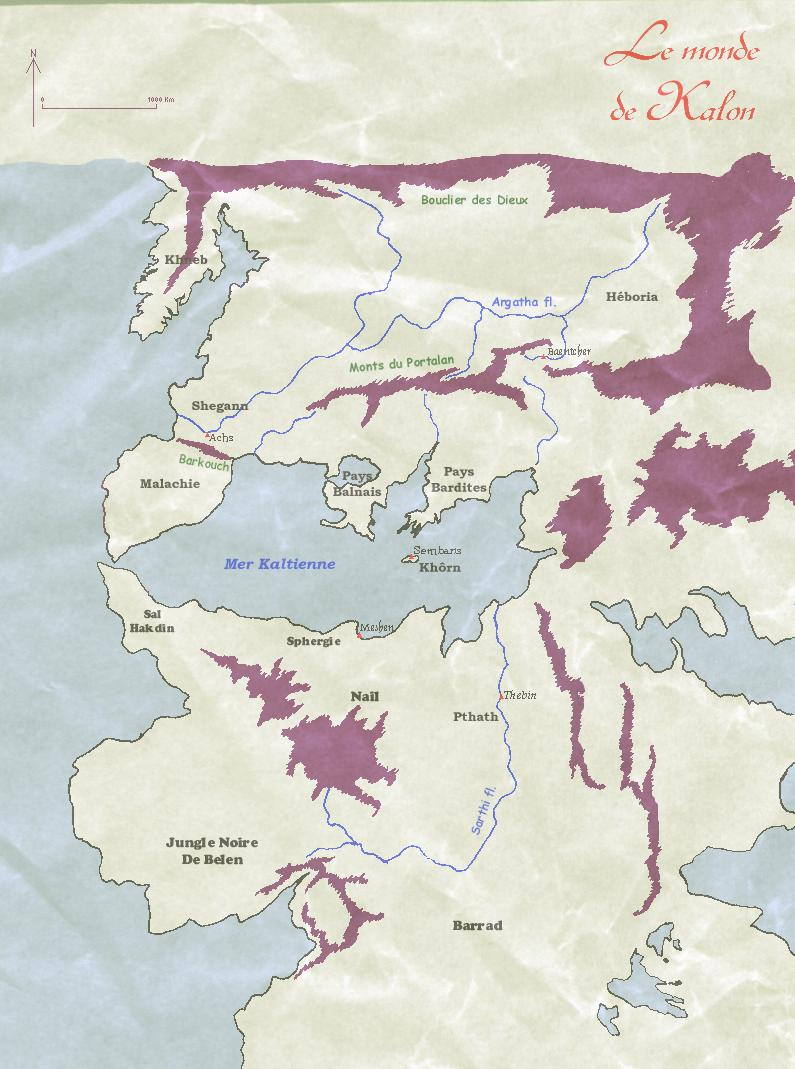
\includegraphics[width=\textwidth]{kalworld.jpg}\\
\footnotesize``Si je comprends bien, �a fait trois semaines qu'on marche en tenant la carte � l'envers?''
\end{center}
%\addtolength{\textheight}{-10cm}


\fancyhead[RO]{\bfseries\textsf{\thepage}}
\fancyhead[RE]{\bfseries\textsf{Les~Aventures~de~Kalon}}
\fancyhead[LO]{\bfseries\textsf{\leftmark}}
\fancyhead[LE]{\bfseries\textsf{\thepage}}
%\fancyhead{} % get rid of headers on plain pages
\renewcommand{\headrulewidth}{0.5pt}
\renewcommand{\footrulewidth}{0pt}

\chapter
[Kalon et l'Ile du Dieu Fou\res{Kalon fait la connaissance de Melgo le voleur, et explore un donjon vicieux.}]
{Kalon et l'Ile du Dieu Fou}
\begin{intro}
KALON I -- Or donc voicy que s'ouvre le livre mill�naire, celui qui narre les aventures de Kalon. Port� vers l'aventure par son caract�re, voici comment il se tire d'une f�cheuse posture et rencontre un compagnon d'armes.
\end{intro}


\section{Les chroniques de l'�ge born�rien}

Entre la chute de l'Empire d'Or et l'av�nement des P�res de Mrryn, alors que les horreurs sans nom du Cycle de Sang n'�taient d�j� plus que l�gendes terrifiantes et que les Dieux A�n�s n'avaient pas encore commenc� � comploter pour leur retour, le monde connut une �re troubl�e appel�e �ge Born�rien.

C'�tait un temps de sorciers et de d�mons, de puissantes forteresses et de hordes innombrables, de fer et de feu, un temps o�, par la ruse, l'adresse ou la force, un homme pouvait se dresser contre le destin et triompher des obstacles mis sur sa route par les dieux ombrageux, un temps o� encore se dressaient les ruines cyclop�ennes des cit�s perdues de Xhan, pleines des cris des �mes supplici�es en ces lieux vingt si�cles plus t�t, de sombres et myst�rieuses for�ts recouvraient alors la Terre et donc le papier ne co�tait pas cher, ce qui explique qu'on y aimait tant les interminables introductions.

Et si un seul nom devait rester de cette �poque, ce serait celui de Kalon.

\section{O� l'on apprend l'histoire de Kalon}

Il avait suivi un cursus somme toute assez classique; apr�s une enfance pleine de jeux virils et m�morables corrections paternelles, il avait accompagn� sa horde qui �pisodiquement �cumait son H�boria natale et les provinces environnantes, ce qui lui avait valu malgr� son jeune �ge une flatteuse r�putation de sombre brute. Puis il avait vu son clan massacr� sous ses yeux par un myst�rieux cavalier � l'armure noire dont, � ses moments perdus, il cherchait � se venger. Men� en d�portation dans les mines de Thendara, il eut tout loisir de cultiver sa musculature avant que des marchands Khn�bites ne le remarquent et ne le rach�tent pour en faire un gladiateur dans une de ces petites ar�nes itin�rantes qui sont la sp�cialit� des terres du nord. Il se perfectionna alors au m�tier des armes, et apprit le peu qu'il savait sur le monde avant de s'�vader et d'embrasser la carri�re de mercenaire dans l'arm�e de Badalos, prince cadet de Melgosia, une petite cit�-�tat assez crasseuse qui, dans la r�gion, passait pour une m�tropole impressionnante. Il prit donc part � sa premi�re guerre, un conflit aussi atroce que bref entre Badalos et son fr�re a�n� dont les enjeux �taient le tr�ne bancal et la couronne oxyd�e de Melgosia.

Le destin voulut qu'il choisisse le camp du vainqueur et c'est fi�rement qu'il entra dans la ville en flammes, � la t�te de la demi-douzaine de bons � rien qu'on lui avait confi�s. Apr�s une semaine de beuveries, l'esprit embrum� par le vin (c'est � dire un petit peu plus embrum� que d'habitude) et suite � un pari d'ivrogne, Kalon succomba aux charmes par ailleurs sujets � controverse de la princesse Zenia, soeur de Badalos. Mais apr�s qu'il lui eut offert d'inoubliables instants de volupt�, il fut surpris par la garde qui ne lui laissa gu�re le temps d'expliquer que la belle ne lui avait pas ferm� la porte (ce qu'en fait il n'avait pas v�rifi�, �tant pass� par la fen�tre), qu'elle s'�tait lascivement alanguie dans ses bras (apr�s qu'il l'eut assomm�e, il est vrai) et qu'elle ne s'�tait pas explicitement refus�e � lui (la pauvrette �tant muette de naissance). Quoi qu'il en soit, Kalon sauta sans blessure aucune de la plus haute tour du palais -- soit, il �tait au premier �tage -- et s'en fut vers le nord o� il savait trouver la For�t des Ombres qui lui fournirait, il y comptait, un abri.

\section{O� notre h�ros �chappe � la mort, du moins temporairement}

Or il se trouvait que la For�t des Ombres avait connu des jours meilleurs. Au temps jadis en effet s'�taient dress�s l�, tels autant de soldats immobiles, titanesques et �ternels, des millions de s�quoias g�ants aux lourdes branches charg�es d'�pines longues et noires et de chatons pelucheux, mais la main avide de l'homme, la mandibule vorace de l'insecte xylophage, � moins que ce ne fussent les pluies acides, avaient ruin� � jamais ces cath�drales de verdure dont il ne subsistait que troncs moisis et bosquets chenus.

Kalon courait donc de toute la vitesse de ses jambes, et dieu sait qu'il pouvait courir vite dans les plaines glac�es d'H�boria, mais le plateau o� il se trouvait �tait accident�, couvert de divers r�sidus v�g�taux et il �tait pieds nus, car ses sandales �taient rest�es dans la chambre de la princesse. Le reste de ses v�tements aussi, d'ailleurs. De toute mani�re, le plus pi�tre cavalier ira toujours plus vite que le meilleur des coureurs, et les Gardes Noirs de Melgosia savent, entre autres choses, monter � cheval. Kalon atteignit un providentiel vallon dont il d�gringola plus qu'il ne d�vala le flanc escarp� et -- miracle -- bois�. Les chiens l'y suivirent bient�t.

Ce qui avait sauv� Kalon jusqu'ici, c'est que le dogue melgosien n'est pas un chien courant, � la base. Trapu, plut�t petit, juch� sur de curieuses pattes arqu�es et rev�tu d'un pelage ras par endroits et inexistant ailleurs, il semblait de prime abord que le cr�ateur ait �t� distrait quand il l'avait con�u. C'�tait faux: en fait, toute son attention �tait concentr�e sur la partie avant, celle qui porte les dents et que, pour simplifier, nous appellerons "t�te". Le dogue melgosien est une machine � mordre, il est connu que lorsqu'il tient une proie entre ses terribles m�choires, seule la mort peut le faire l�cher prise. On connaissait du reste des cas o� la mort n'avait pas suffit.

En bas dans le ravin, coulait un ruisseau, ce qui est g�od�siquement assez coh�rent. Les chiens s'arr�t�rent sur la rive, travers�rent dans les deux sens, coururent en rond et g�mirent en attendant que leurs ma�tres cavaliers arrivent.

-- Il a d� descendre le long du ravin, sire, pour troubler les chiens, fit le capitaine de la garde, martial.

-- Ou bien le remonter, nota le roi, maussade. Il se serait bien pass� de cette exp�dition punitive dans la campagne, il y avait tant � faire en ces lendemains de victoire. Heureusement qu'il pouvait compter sur un bourreau d�vou� et dur � la t�che.

-- Habituellement, sire, les animaux sauvages pris dans une telle situation descendent les rivi�res, ils vont plus vite.

-- Et ils se font prendre car tous les chasseurs connaissent le coup. Notre homme est rus�, il a du souffle, il a du aller en amont pour nous tromper. En avant!

Et les chevaux repartirent dans de grandes gerbes de boue et d'eau glac�e.

Badalos �tait un aristocrate volontaire et intelligent, mais avait cependant un d�faut, bien excusable vu son m�tier : il m�prisait au plus haut point les gens du commun, auxquels il se m�lait le moins possible, pr�f�rant frayer avec les gens de sa caste car parfois ils se lavent. Ainsi durant la guerre �clair qui l'avait port� sur le tr�ne, avait-il peu fr�quent� sa propre arm�e, et encore moins les mercenaires barbares qu'il avait engag�s. L'eut-il fait qu'il se fut vite rendu compte d'une �trange particularit� anatomique: la cervelle de Kalon �tait aussi lisse que son biceps �tait noueux.

Notre h�ros avait en effet suivi sans se poser de question tout � la fois son instinct et la pente, ce qui l'avait conduit au bord d'un lac. L'endroit �tait inqui�tant, rien ne poussait sur la berge boueuse qu'on eut pu appeler plante sans offenser mortellement la gent v�g�tale, une brume matinale flottait au-dessus de l'eau, lui donnant une teinte gris�tre et brouillant avec juste raison la forme hideuse d'une �le tourment�e, au large. A un jet de pierre des premi�res vases �merg�es, une barque minuscule au bois noirci par la putr�faction servait de support � un personnage vo�t�, enti�rement recouvert d'un manteau noir et tenant une longue gaffe dans sa main gant�e\footnote{De noir, mais fallait-il le pr�ciser?}. Sa capuche baiss�e ne laissait rien voir de son visage, et sans doute �tait-ce mieux ainsi. Kalon sauta prestement sur la barque d'une stabilit� �tonnante pour sa taille, et ordonna au passeur de sa puissante voix:

-- L�-bas !

Il d�signait l'�le sombre d'un index imp�rieux.

Et le passeur appuya sur sa gaffe, propulsant son embarcation � une vitesse surprenante. Ils n'�taient d�j� plus � port�e de fl�ches lorsque les cavaliers et leurs chiens d�boul�rent sur la rive et Kalon, debout � l'arri�re du fr�le esquif, les salua de son regard de fer et d'un vigoureux bras d'honneur. Peut-�tre aurait-il �t� moins fier s'il avait pu entendre le rire du roi Badalos et de ses gardes, peut-�tre aurait-il �t� plus prudent s'il s'�tait demand� pourquoi un passeur attendait � cet endroit o�, manifestement, aucune route ne menait, mais insouciant et confiant en son destin, Kalon d'H�boria filait sur l'eau vers l'�le du Dieu Fou.

\section{O� l'on d�couvre l'�le maudite de Lowyn}


C'�tait une terre d'une d�solation comme peu de gens en ont jamais con\-tem\-pl�e: une terre caillouteuse et infertile, noire comme la mort et dont semblaient suinter des exhalaisons m�phitiques et impies que m�me l'�me lourde de notre barbare ne pouvait ignorer, parsem�e d'innombrables dalles bris�es ou couch�es dans lesquelles on reconnaissait des tombes anciennes, sans nom. Pris d'une compr�hensible h�sitation, il fit demi-tour pour constater que d�j� le passeur avait disparu dans la brume qui soudain s'�tait �paissie.

Alors il marcha sur l'�le � la recherche d'un abri, d'armes, de v�tements et d'un bateau pour rejoindre un rivage plus accueillant. Il marcha longtemps car l'�le �tait vaste et, partout, se dressait le m�me cimeti�re, sinistre et glac�, que nul renard, nul passereau ne venait r�clamer comme son territoire. La brume lui cachait m�me le soleil et il se retrouva, apr�s une heure, sur un rivage qui lui �tait familier puisque c'�tait celui qu'il avait quitt� un peu plus t�t.
Notre h�ros commen�a alors � perdre le contr�le de lui-m�me. Certes les natifs d'H�boria sont de rudes gaillards � l'�me bien tremp�e, habitu�s aux longues randonn�es solitaires dans les contr�es hostiles, combattants � la bravoure reconnue, n'h�sitant gu�re � attaquer les monstres les plus hideux des montagnes bor�ales ou les redoutables tribus masqu�es de Blov dont le nom fait fr�mir les plus t�m�raires, mais la magie est rare dans les terres du nord et ses habitants sont superstitieux au plus haut point. Kalon l'inflexible commen�ait donc � prendre peur. Et lorsque de la brume se form�rent autour de lui de curieux tourbillons muets, son coeur se gla�a et ses membres se paralys�rent. Les tourbillons prirent forme presque humaine tandis que dans les oreilles de notre h�ros, les battements fr�n�tiques de son propre coeur firent place � une musique comme il n'en avait jamais entendue, un petit air de fl�te � la fois espi�gle et lourd de menaces innommables. Alors les spectres parl�rent � Kalon:

-- Fuis, h�ros, fuis l'�le du Dieu Fou.

Une autre voix derri�re lui:

-- La mort t'attend sur l'�le de Lowyn, fuis si tu veux vivre, et oublie le glaive si tu ne veux pas nous rejoindre.

Une pr�sence f�minine, pr�s de son oreille gauche:

-- Donne-moi ta vie, guerrier, donne-moi ta chaleur...

Mais d�j� Kalon avait retrouv� sa mobilit� et travers� en hurlant le cercle des �mes errantes, courant loin devant lui, loin des spectres qui le mettaient en garde.

Il n'arr�ta sa course folle que quand il heurta le mur d'une grande tour.


\section{O� l'on rencontre Melgo le voleur}


Le coup lui avait fait reprendre ses esprits et notre h�ros, le coeur battant, allong� dans l'herbe rare, pouvait admirer la haute silhouette d'un grand �difice carr� dont le sommet se perdait dans les brumes. La pierre en �tait noire et gluante d'une sorte de lichen humide et malsain qui semblait la manger jusqu'aux tr�fonds. Le barbare sauta prestement sur ses pieds, consid�ra longuement la tour qu'il n'avait jusque l� pas vue, se demandant � peine comment une telle construction avait pu lui �chapper. Pensant trouver un abri s�r, Kalon fit donc le tour du b�timent et finit par trouver une porte de bois lourd et noir, orn�e de motifs de bronze pass�s et us�s dont le sujet n'est pas racontable ici. La porte �tait entrouverte et un curieux m�canisme �tait engag� dans sa serrure. Il la poussa sans difficult� et p�n�tra sans h�siter dans les t�n�bres. L'�cho du bruit de ses pas renseigna ses oreilles entra�n�es sur les dimensions de cette salle, qui devait occuper tout le rez-de-chauss�e de la tour, le plafond quand � lui �tait trop haut pour �tre d�celable. Il attendit, immobile, que ses yeux s'habituent � l'obscurit� et huma l'air pour passer le temps. Il enregistra, par dessus les relents de putr�faction habituels de l'�le, une odeur de fum�e qui mit un certain temps pour arriver jusqu'� son cerveau.

-- Y'a quelqu'un ?

-- Toi aussi, tu viens pour le tr�sor du Dieu Fou?

Entre le barbare et la porte, dans un silence absolu, s'�tait gliss� un homme d'assez petite taille, enroul� dans une cape sombre. Kalon ne voyait de lui que la silhouette trapue et la longue lame d'acier d'une rapi�re soigneusement polie. Sa voix, extraordinairement douce et calme, inspirait la confiance et la bont�. Tout dans sa mise et son attitude trahissait le voleur professionnel. Kalon se demanda de longues secondes durant de quel tr�sor parlait le petit homme, puis d�cida de jouer la subtilit�.

-- Ouais.

Le voleur se maudit d'avoir aussi stupidement d�voil� la raison de sa pr�sence � ce sauvage nu et d�sarm� qui, visiblement, n'avait jamais entendu parler du Dieu Fou ni des secrets de son antre, c'�tait � se frapper la t�te contre les murs. Puis les enseignements de son vieux ma�tre lui revinrent en m�moire. Le sage disait ``Lorsque le destin met une pierre sur ton chemin, demande-toi si tu ne peux pas la jeter � la t�te de ton ennemi''. Car apr�s avoir d�ploy� tout son art dans le crochetage de la serrure d'entr�e, qui �tait bourr�e d'aiguilles empoisonn�es, d'acides divers et de pi�ges subtils, notre homme se retrouvait maintenant bloqu� par un obstacle d'une stupidit� peu commune, et la brute qui venait d'appara�tre lui semblait maintenant un cadeau envoy� par Xyf, dieu des voleurs et des marchands, pour le r�compenser de ses efforts.

-- Que dirais-tu d'unir tes forces aux miennes, si la l�gende dit vrai nous ne serons pas trop de deux pour vaincre les p�rils qui nous attendent dans les caves de la tour, et il y a bien assez de tr�sors pour faire notre bonheur. 

Kalon, n'ayant rien de mieux � faire ce jour-l� et int�ress� par la perspective de gains rapides et faciles, ne se le fit pas dire deux fois.

-- Ouais.

-- Je suis Melgo, ``n�gociant'' de Pthath. Petite est ma taille mais grandes sont ma ruse, mon audace et mon intelligence. Nul mieux que moi ne manie � la fois le verbe et l'espadon dans les contr�es septentrionales, et le r�cit de mes exploits a fait le tour de toutes les tavernes du monde. Certains me nomment ami, fr�re, compagnon, d'autres maudissent le jour o� ma truie de m�re se livra � mon chien de p�re contre quelques bagolles\footnote{La bagolle est une monnaie de cuivre qui a cours dans certains quartiers de Th�bin, capitale de l'Empire de Pthath, les jours ouvr�s pairs de toutes les ann�es non bissextiles. Il faut g�n�ralement treize bagolles et un tiers pour faire trois quarts de Malpon d'argent.}, mais tous s'accordent � le dire, et moi le premier, je suis voleur et j'en suis bien aise.

-- Kalon, H�borien.

-- Pas bavard hein, tant pis, je le suis pour deux, � ce qu'on dit. Comme tu as pu le voir j'ai, en d�ployant des tr�sors de dext�rit� et d'astuce, ouvert la Porte de Bronze des Amiti�s Animales dont parle la l�gende, et je m'appr�tais � soulever cette dalle qui, je le pense, nous m�nera au Couloir des Peines Profondes. Veux-tu m'aider?

-- Ouais.

Le voleur alluma une torche et d�signa un endroit du sol. Melgo �tait, comme on l'a dit, de taille fort moyenne, ce qui est plut�t un avantage dans une profession o� il est courant de devoir se glisser dans des endroits �troits, se cacher et passer inaper�u. A ce titre il �tait favoris� par son physique, qui ne pr�sentait ni gr�ce particuli�re ni laideur notable, un t�moin aurait donc �t� bien en peine de le d�crire. Peut-�tre son regard noir et inquisiteur ou sa calvitie naissante auraient-elles pu attirer l'attention de quelqu'un d'observateur, et encore. Disons simplement qu'il avait les cheveux bruns et longs attach�s par un catogan, mais il changeait souvent de coiffure, le teint mat des gens du sud, qui pouvait passer pour le bronzage d'un paysan, et qu'on lui donnait en g�n�ral dans les trente ans. Cela faisait six heures qu'il s'escrimait � tirer l'anneau de bronze fix� � l'�norme dalle orn�e de gravures hideuses qui occupait le centre de la salle, sans arriver � l'�branler un instant. Il avait m�me un instant song� � faire demi-tour pour chercher des renforts en Sellygie, quitte � d�clarer ce vol � la Guilde des Voleurs locale. La r�ponse laconique de l'H�borien le remplit d'une exultation qu'il eut du mal � dissimuler, malgr� de longues ann�e d'�tudes et un certificat d'escroquerie du deuxi�me degr� obtenu avec mention bien; vu la carrure de son nouvel alli�, nul doute qu'il parviendrait � ouvrir le passage. Car notre h�ros �tait exceptionnellement bien b�ti: mesurant plus de seize pouces et deux pieds de haut pour trois aunes et un empan de large, il avait plus de mal � passer dans les portes qu'� se faire remarquer en soci�t�. Notons au passage que ces mensurations sont � comprendre en pouces Khn�bites, pris � partir du gros orteil du prince Mulittzar l'Ecrase-Merde (1 pK = 14,09 cm), en pieds Volhards, mesur�s sur le foetus momifi� de Volhard V, Celui-Qui-Aurait-D�-Etre-Le-Fl�au-Du-Monde (1 PV = 3,75 cm), en aunes de Baal-Nezbett (soient dix-sept et trois-quarts de fois moins que la hauteur du Temple Titanique de la Foi �ternelle de Bel-Shamaroth apr�s le tremblement de terre qui le ravagea en 704, 1 aBN = 38,77 cm), et en Empans Sacr�s de Poualla (1 ESP = 14,25 cm)\footnote{Les mesures sont en centim�tres R�galiens, sous-multiples du m�tre R�galien, unit� qui varie, comme chacun sait, selon que la longueur mesur�e est horizontale, verticale, oblique ou curviligne selon le principe d'absconcit� maximale de Kubonal, le Phol Fysicien.}.

Kalon avait donc le physique que l'on �tait en droit d'attendre d'un H�borien, une chevelure noire comme la nuit mettant en valeur son �chine musculeuse, des membres solides comme des colonnes de marbre, un torse rappelant le tronc d'un ch�ne et un visage dur comme les glaciers du Bouclier des Dieux.

\section{O� nos amis d�jouent quelques pi�ges de fa�on peu orthodoxe}


Donc, Kalon s'approcha, s'accroupit, prit la poign�e � deux mains et commen�a � tirer de toutes ses forces. Il ne fallut gu�re de temps pour que la pierre c�de et se soul�ve dans un fracas de tonnerre, r�pandant autour d'elle mille cailloux et fragments aigus, ainsi que de consid�rables quantit�s d'une poussi�re s�che et malodorante. Consid�rant la puissance �tonnante de son partenaire, Melgo commen�a � douter de l'opportunit� de l'�gorger une fois le tr�sor trouv�, comme il en avait tout d'abord eu l'intention. Kalon regardait maintenant l'orifice carr� d'un air bovin. Une vol�e de marches abruptes taill�es dans le roc massif s'enfon�aient dans le sol jusqu'� une petite pi�ce qu'on devinait p�niblement � la lueur de la torche. Ce fut lui qui descendit le premier, lentement, attentif au moindre bruit, � la plus petite d�clivit�, � un quelconque signe qui pourrait trahir la pr�sence d'un pi�ge ou d'un ennemi dissimul�. La cave �tait basse, vo�t�e, son sol �tait de terre battue et sur le mur oppos� � l'escalier, les feux dansants de la torche accrochaient les argents d'une porte massive, orn�e h�las des m�mes types de dessins que la porte d'entr�e.

-- La Porte d'Argent des Amiti�s Animales, la l�gende dit qu'elle rec�le un pi�ge encore plus dangereux que la premi�re.

-- Ah, fit le barbare avant de bondir sur la porte et d'y donna un grand coup de pied. Elle se brisa en plusieurs endroits et des morceaux de bois pourri et vermoulu vol�rent de l'autre c�t�, dans un couloir long et �troit. Melgo examina les d�bris de la serrure, constatant qu'effectivement le second pi�ge �tait plus subtil encore que celui qu'il avait d�jou� quelques heures auparavant, puis releva la t�te et ses yeux s'agrandirent d'effroi: Kalon, qui s'�tait avanc� dans le couloir, s'appr�tait � marcher sur une dalle l�g�rement plus grande que les autres, l�g�rement plus basse, l�g�rement mieux taill�e... Bien s�r, ses yeux de voleur exp�riment�, qualifi�, dipl�m� et pr�bend� avaient imm�diatement rep�r� le pi�ge, sans doute quelque trappe insondable garnie de pieux barbel�s, empoisonn�s, explosifs, maudits et rouill�s, comme elles le sont toutes.

-- Ne bouge plus, Kalon!

-- Hein?

Et Melgo s'aper�ut que sa langue l'avait trahi une seconde fois. Qu'avait-il donc pr�venu ce barbare du destin funeste qui l'attendait, ce pi�ge sans doute l'aurait d�barrass� d'un alli�, toujours encombrant au moment du partage, et quand bien m�me aurait-il surv�cu que Kalon n'aurait eu aucun motif de lui en tenir rigueur. Mais il �tait trop tard maintenant, et le rus� -- mais pas trop -- Melgo, ne voulant pas prendre de risque, indiqua le pi�ge � son compagnon d'aventure. Celui-ci, incr�dule, voulut faire un essai. Il retourna vers la porte, en arracha un lourd fragment de bois qui pendait encore � un gond et le lan�a sur la dalle suspecte. Elle bascula avec le cliquetis d'une m�canique bien huil�e, laissant choir le morceau de bois dans une fosse carr�e dont on ne voyait pas le fond. Apr�s quelques secondes, on entendit un choc suivi d'une s�rie d'explosions, et quelques lamelles de fer oxyd� et enduites d'une substance verd�tre et gluante vinrent se ficher en sifflant dans le plafond vo�t� du couloir.

-- Oh !

-- Bien. Je crois que ce pi�ge est d�samorc�. Continuons, mon ami.

Kalon, vaguement conscient d'avoir une dette envers le voleur, d�cida qu'il �tait temps de l'impressionner par une performance physique. C'est toujours ainsi qu'il agissait lorsqu'on d�couvrait la pauvret� de son intellect, il cherchait � compenser sa faiblesse par un coup d'�clat qui faisait taire les moqueurs, du moins lorsqu'il �tait pr�sent. C'�tait une attitude naturelle, inconsciente mais qui lui avait toujours r�ussi. La fosse mesurait environ quatre aunes de Baal-Nezbett, c'est-�-dire qu'un enfant de dix ans pas trop souffreteux aurait pu la franchir sans peine, mais Kalon n'en recula pas moins jusqu'� l'ex-Porte d'Argent des Amiti�s Animales, courut d'une foul�e aussi puissante qu'�l�gante et, d'un bond gracieux autant qu'inutile, enjamba plus du triple de la longueur de l'obstacle. Il retomba lourdement, plut�t content de sa performance, avant de se retourner, souriant triomphalement � Melgo qui jugea avis� de f�liciter chaudement son compagnon. Il prit � son tour son �lan et chut quelques pouces (Khn�bites) au-del� du bord de la trappe.

A l'instant o� son pied toucha le sol, il sentit que quelque chose clochait. Nul doute que si , dans le calme de la salle d'�tude de sa guilde, quelque ma�tre-voleur retors lui avait d�crit une telle situation, il aurait soup�onn� une quelconque rouerie de la part de l'architecte qui avait con�u une si pi�tre trappe dans un souterrain sens� abriter un dieu. Nul doute qui si, quelques ann�es auparavant, il avait assist� au cours intitul� ``la double-trappe de Moggen, principe, usage et histoire'' au lieu de courir la gueuse dans les tavernes de Th�bin, il aurait r�fl�chi � deux fois avant de sauter b�tement � la suite du barbare. Mais c'�tait trop tard, et la dalle bien cach�e sur laquelle il se trouvait basculait maintenant, l'entra�nant vers des profondeurs qu'il imaginait lointaines et inhospitali�res.

Et alors qu'il s'appr�tait � rencontrer Xyf, son dieu, apr�s une d�plaisante mais courte agonie sur les pieux explosifs, empoisonn�s, maudits, barbel�s et rouill�s qu'il savait trouver en bas, la main puissante et calleuse de Kalon l'H�borien agrippa son poignet et le tira prestement du trou, lui d�bo�tant un peu l'�paule par la m�me occasion.

-- Merci, H�borien, maintenant nous sommes fr�res de sang et si un jour...

-- Ouais, fit le barbare, qui �tait peu enclin aux serments �ternels et viriles accolades, habituelles en de telles circonstances.

Et nos amis, sans �changer d'autres mots, reprirent plus lentement leur progression le long du Couloir des Peines Profondes, Melgo passant en premier avec la torche, attentif � la moindre asp�rit� de la roche. D'apr�s la l�gende, la Porte d'Or des Amiti�s Animales �tait d�fendue par une rune magique particuli�rement meurtri�re, sur laquelle Melgo avait plus ou moins compt� pour se d�barrasser de Kalon. Mais de la porte il ne restait que quelques �chardes humides, des gonds monstrueusement gonfl�s par la rouille pendant lamentablement dans l'encadrement et quatre plaques d'acier poli sur une face et dor� sur l'autre, repr�sentant ce que vous devinez, jonchant lamentablement le sol depuis des �ons. La rune, � la longue, avait d� ronger le bois, l'enchanteur ne devant pas �tre tr�s consciencieux.

Derri�re feue la porte, le couloir faisait un coude et nos amis devinaient comme un air lointain, le son d'un fl�tiau aigrelet �grenant quelque �trange m�lop�e semblant venue de la nuit des temps, de quelque civilisation oubli�e, une musique � la fois espi�gle et pleine de menaces voil�es et de hideux sous-entendus. Un rougeoiement inqui�tant �manait de l'endroit dont, avec quelque appr�hension, nos h�ros approchaient. Kalon se glissa le long du mur, d'une d�marche f�line et silencieuse, h�sita quelques secondes, puis risqua un rapide coup d'oeil.

\section{O� l'on d�couvre avec horreur l'antre du Dieu Fou}


Dans une grande pi�ce circulaire, sous une vo�te unique et puissante, quatre torches fich�es dans le murs �clairaient, ou plut�t soulignaient les ombres des nombreux objets qui encombraient le sol dall� et poussi�reux. Un autel de pierre p�le, haut comme la moiti� d'un homme, repr�sentait un veau monstrueux � six pattes et deux t�tes. Le dos de l'animal semblait plus sombre et z�br� de stries minuscules. A une corne pendait une forme sombre et velue que Kalon souleva. C'�tait un v�tement de peau de b�te humide et infest� de vermine, qui se d�chira et tomba par terre dans un bruit mou et �coeurant. Diverses pi�ces d'�toffe, ou ce qui y ressemblait, achevaient de moisir en de multiples petits tas indistincts et dispers�s. A l'autre bout de la salle, contre le mur, se dressait un monticule de ce que nos amis pr�f�r�rent prendre pour des branchages blancs et secs, parfois recouverts de pi�ces de cuir noirci. La musique venait apparemment d'une statue de faune dansant et jouant de la fl�te de pan, de la m�me pierre que l'autel, et qui gisait renvers�e devant l'entr�e. Derri�re, le squelette de quelque malheureux gisait, grotesquement affal� sur un coffre �ventr� laissant �chapper son contenu de pi�ces d'or, d'argent et de cuivre. Les v�tements du mort �taient depuis longtemps tomb�s en poussi�re, et seul l'arceau et les attaches rouill�es de son bouclier attestaient qu'il en avait eu un. Son �p�e par contre avait r�sist� � l'assaut du temps et � la corruption de ce lieu sinistre. Un miroir enfin, ovale, massif, plus grand que Kalon, encadr� d'un support de bronze poli dont les ornements rappelaient sans nul doute ceux des trois portes, tr�nait au centre de la pi�ce, irradiant le mal�fice.

Sans plus attendre ni se poser de question, les deux hommes se pr�cipit�rent vers le coffre avec l'instinct que donne de longues ann�es de rapines. Melgo balaya le squelette d'un revers de la botte et acheva de briser le bois vermoulu � coups de pieds. Puis il s'agenouilla dans le tas de pi�ces et en jeta de pleines brass�es en l'air, riant et poussant de petits cris.

-- Nous voil� riches, Kalon, riches comme des rois. Regarde tout cet or...

Kalon �tait quant � lui plus sobre dans son triomphe, il s'�tait empar� de la lourde �p�e d'acier poli et la contemplait avec des yeux ronds depuis de longues secondes, la tournant lentement dans ses mains expertes afin d'admirer tous les reflets subtils de la longue lame. Par instant la lumi�re semblait danser non � la surface, mais � l'int�rieur m�me du m�tal.

C'est � ce moment qu'une des cornes du veau � deux t�tes se d�tacha et se fracassa par terre, pr�venant providentiellement nos piteux h�ros du p�ril qui les mena�ait: le grand miroir �mettait une vapeur noire et grasse qui coulait sur le sol telle une mar�e immonde venue d'une autre r�alit� tandis que la glace se troublait, laissant entrevoir quelque forme encore indistincte mais qui, en se pr�cisant peu � peu, ne gagnait gu�re du point de vue esth�tique.

Une main ou une patte griffue sortit du miroir et saisit l'encadrement, une sorte de pied caoutchouteux se posa sur le sol qui se mit imm�diatement � grouiller d'une vermine sortie d'on ne sait o�. Enfin �mergea, au bout d'un long cou parchemin� et gangr�neux, une t�te qui semblait issue du croisement d'une limace, d'une mouche et d'un ustensile de bourreau. La cr�ature se d�gagea avec peine des flux d'�nergie magique qui l'environnaient, s'�broua en un frisson et tourna sa t�te de cauchemar vers Kalon et Melgo p�trifi�s. Ils se sentirent alors repouss�s par une aura de puissance et de mal�volence peu commune, � moins que ce ne fut par l'odeur de la b�te, qui rappelait assez celle des latrines de la prison de Nolab'Hazn la cit� des mendiants apr�s l'�pid�mie de chol�ra de 709.

-- MORTHELS, PHREPAREZ-V�OS A AFFR�NTER V�TRE DESSTIN. TRO�\-VEZ L� REPHONSE A MONNN ENIGHME ET JE V�OS AC\-KOR\-DHE LA GRASS D'�N M�ORT RAPYIDE.

-- Ah, et si on ne trouve pas ? demanda Melgo en ma�trisant un tremblement.

-- NHIIYGHA VNHY VNHY VNHY VNHY !

Il fallut un certain temps aux deux hommes horrifi�s pour comprendre que la cr�ature, dans une tentative path�tique pour singer un comportement humain, riait.

-- VOICYI L'ENIGHME: KHELLE ETHRANGE CREATH�RE SUIS-JE DONKH, KHYI LE MATTIN MARSH S�R KHATTRE PATTHES, � MYIDYI S�R DEUX ET LE SO�AR S�R THRO�AA ?

-- C'est facile, s'�cria Melgo, soulag�. C'est l'homme, qui au matin de sa...

-- PHERD� !

-- Quoi perdu, mais c'est la vieille �nigme des Dippes, tout le monde la conna�t! Je proteste!

-- LA REPHONSS K�RRECKQTH ETAIT: LA GERBO�ZE CREPH�E DU HAUT-MEDDOCKQ. JE VAIS D�NCK V�OS DEV�RRER T�OS DEUX ET V�S CORR SE DISSOUDRONN LENTEMANT D�NS MES SUCKS DYIJJESTIFS THANDYIS KHE V�S �MES G�HIR�ONT MILLE SIECLES D�RANT DANS LES S�OMBRES ABY�MMES DE XHNT'HAHNS.

Le monstre se contourna d'�coeurante fa�on et se jeta sur Kalon qui jusque-l� �tait rest� p�trifi� de terreur. La b�te avait opt� pour le barbare car il �tait plus gros, et surtout il n'�tait pas emmaillot� dans des �paisseurs de tissus poisseux et de m�tal croquant comme les hommes en avaient la d�testable habitude. Ces d�tails ont leur importance quand on n'a rien mang� depuis cent quarante ans.

Donc le monstre rampa vers sa cible apeur�e, s'attendant � une victoire rapide sur un aussi pi�tre bip�de, et sourit int�rieurement (car ext�rieurement, il n'�tait pas �quip� pour) de le voir lancer sur lui sa seule arme, son �p�e, dans un geste d�sesp�r�. Il se d�materialisa, sentit avec d�lice l'arme lui chatouiller les organes internes (on a les plaisirs qu'on peut) et se remat�rialisa pour reprendre son assaut sur le massif primate. Mais un bruit de verre bris� lui rappela un d�tail horriblement g�nant que le go�t du sang lui avait fait oublier: le miroir �tait derri�re lui, et il �tait assez fragile.

Melgo vit le monstre s'agiter, changer de forme, une multitude d'�ph�m�res bubons couvrirent sa peau noir�tre avant de crever en autant de gerbes de pus, de liquides organiques divers et de gaz multicolores tout en �mettant des sons suraigus � vous vriller la glande pin�ale. Le voleur crut d'abord � une ultime manifestation de puissance de la cr�ature avant l'assaut final, mais lorsque l'atroce hurlement d�crut, il dut se rendre � l'�vidence: la chose, sans son miroir, agonisait.

Ce n'est qu'apr�s plusieurs minutes, lorsque la b�te se fut tue � jamais et que les restes racornis de son corps ne furent plus qu'une tache aplatie sur le sol tout juste agit�e de petits ``Plops'' sporadiques, que nos h�ros se relev�rent, encore passablement h�b�t�s.

-- Kalon, puissant guerrier, je loue Xyf mon dieu de t'avoir plac� sur ma route et de ne pas avoir fait de moi ton ennemi. Je vois que ta sagesse �gale bien ta force. Mais comment as-tu fait pour deviner le point faible de cette cr�ature?

-- Ben, euh, je sais pas.

-- Et en plus tu es modeste! Je chanterai d�sormais tes louanges chaque jour que Xyf me pr�tera vie et dans toutes les tavernes de l'univers. B�ni soit le jour o� je t'ai rencontr�, mon ami.

Et donc Kalon l'H�borien, fils de Lochnar Torse Velu et de S�mia la Louve, et Melgo de Pthath, fils de deux individus de sexe diff�rent, partag�rent �\-qui\-ta\-ble\-ment le tr�sor du dieu fou qui se montait � sept livres d'or, douze d'argent, huit de cuivre (en monnaies diverses, dont la plupart n'avaient plus cours depuis des si�cles), quelques menues pierres pr�cieuses et une �p�e (que Kalon emporta et appela doctement ``l'exterminatrice''). Lorsqu'ils sortirent de la tour mal�fique, la brume s'�tait lev�e et un soleil magnifique �clairait le lac de toute sa force, permettant d'admirer un paysage de toute beaut�. Ils emprunt�rent la barque de Melgo, qui �tait amarr�e au nord de l'�le et ils prirent la direction de la Sellygie pour y faire ripaille et y qu�rir la bagarre. Ainsi se termine la premi�re aventure de Kalon. Mais...

%% \begin{outro}
%% \outtext{Kalon will be back soon in :}{Kalon et la Sorci�re Sombre}
%% \end{outro}
\chapter
[Kalon et la Sorci�re Sombre\res{Le bref passage de Kalon et Melgo en la ville d'Achs laisse � ses citoyens un souvenir imp�rissable.}]
{Kalon et la Sorci�re Sombre}
\begin{intro}
KALON II -- Un guerrier, un voleur... eh, mais il n'y a donc personne pour lancer les projectiles magiques? Kalon et Melgo vont rem�dier � cette situation en la ville d'Achs, centre commercial fort anim�, o� l'on trouve de tout et � tous les prix, y compris de joyeux compagnons.
\end{intro}

\section{O� l'on raconte bri�vement ce qui s'est produit depuis le dernier �pisode}

Kalon, le g�ant H�borien � l'intellect chenu, et Melgo, le voleur Pthaths � la douteuse g�n�alogie, avaient quitt� sans regrets l'�le maudite de Lowyn et la sinistre tour du Dieu Fou, riches d'exp�rience et d'une petite fortune qu'ils se faisaient forts de d�penser � Galdamas, cit� marchande d'importance douteuse au sud du petit royaume de Sellygie. La Sellygie �tait alors un pays � moiti� civilis�, o� les coutumes commer�antes des m�ridionaux avaient certes cours, mais depuis peu de temps, si bien que les autochtones n'en avaient pas forc�ment int�gr� toutes les subtilit�s. Le baron de Galdamas, qui ne rentrera certes pas dans l'histoire comme un des grands th�oriciens de l'�conomie moderne, avait par exemple une notion assez personnelle de la propri�t� priv�e, qui pouvait s'�noncer comme suit : est ma propri�t� priv�e tout ce qui rentre dans les murs de ma cit� et qui a plus de valeur qu'une brouette de fumier. La puissance de cette th�orie avait frapp� nos h�ros, par le truchement il est vrai des neuf gaillards bien b�tis formant la garde personnelle du Baron, et ils ne s'�taient sortis de ce mauvais pas que gr�ce � leur habilet� � l'�p�e, l'esquive et la course. Ils avaient pu sauver de cette piteuse aventure une douzaine de pi�ces d'or cousues dans le revers de la cape de Melgo, des v�tements neufs achet�s par Kalon, l'excellente �p�e trouv�e dans la Tour du Dieu Fou -- que l'H�borien se piquait d'appeler ``l'�corcheuse'' -- et deux petits chevaux des steppes vol�s dans les �curies du Baron. Prenant alors la direction du sud-ouest, descendant le long du puissant fleuve Argatha, ils travers�rent les tristes prairies de Bane, Lasmes, Aliskos et autres minuscules royaumes guerriers dont la pauvret� n'attira gu�re nos ambitieux voleurs, et apr�s un mois de voyage et de menus larcins, que la honte et l'int�r�t du r�cit m'interdisent de vous narrer, ils arriv�rent en vue d'Achs.


\section{O� l'on d�couvre Achs la puissante, porte du Septentrion, et o� l'on se livre � diverses consid�rations sur l'infrastructure h�teli�re}

C'�tait, et de fort loin, la plus grande ville que Kalon ait jamais vu. Il fit son possible pour ne pas para�tre impressionn� aux yeux de son camarade, mais y parvint assez mal. Il est vrai que Melgo lui-m�me, bien qu'�lev� dans les prodigieuses m�tropoles de Pthath, ne put qu'admirer la puissance de la double enceinte, des mille tours cr�nel�es et des innombrables pals en bois de sapin - parmi lesquels beaucoup �taient garnis -- qui avaient fait fuir plus d'un conqu�rant et plus d'un pillard. De petites maisons de pierres massives aux toits d'ardoise lourde se blottissaient frileusement les unes contre les autres, ne laissant que peu de place aux vents de ce d�but d'hiver pour s'engouffrer en hurlant dans les ruelles tortueuses. Achs ne semblait donc gu�re accueillante pour les �trangers, c'est pourtant le commerce qui avait fait sa fortune, vins, huiles, �pices et draperies remontaient des royaumes bordant la mer Kaltienne et s'�changeaient ici contre l'or, les pierres, les chevaux et les esclaves venus des sauvages contr�es septentrionales. D'ailleurs, malgr� l'heure tardive, on voyait encore de nombreuses caravanes arriver de la plaine et faire la queue devant les octrois, crois�es par les charrettes de quelques paysans des alentours s'en retournant � leur campagne apr�s avoir vendu le fruit de leur travail le matin et s'�tre copieusement avin�s l'apr�s-midi.

Il faisait presque nuit quand ils arriv�rent aux faubourgs boueux d'Achs, et bien que les portes fussent encore ouvertes, nos comp�res d�cid�rent d'attendre le lendemain pour faire leur entr�e dans la ville, pr�f�rant coucher dans une petite auberge qui ne payait gu�re de mine, mais o� ils pourraient sans doute glaner quelques renseignements sur les usages d'Achs, les personnages influents, les fortunes � piller et les employeurs potentiels. Lorsque Kalon poussa la porte du ``cochon noir'', la musique langoureuse d'un joueur de zmol -- un compromis entre biniou et fl�te de Pan -- et les senteurs enivrantes des �tranges herbes � fumer venues des lointains pays Balnais l'assaillirent en m�me temps qu'elles renseignaient Melgo sur le type d'auberge dont il s'agissait.

Car apprenez que dans tout l'univers il n'existe que trois cat�gories d'auberges, class�es selon la client�le qui les fr�quente et les services qui y sont fournis.

-- L'auberge de cat�gorie 1 est un lieu de passage essentiellement utilis� par des marchands de petite et moyenne extraction. La nourriture y est passable, voire bonne, les lits infest�s de punaises et d'autres clients arriv�s avant vous, les prix y sont raisonnables. La seule distraction propos�e par ce genre d'�tablissement est la fille de l'aubergiste, invariablement gironde et peu farouche. Le tenancier est quant � lui, en toutes circonstances et quel que soit son sexe, un individu gras, rougeaud, souvent moustachu, qui passe la quasi-totalit� de ses journ�es � essuyer le m�me verre avec le m�me torchon, activit� incommensurablement ennuyeuse qui explique qu'il ne se fasse jamais prier pour discuter avec le voyageur.

-- L'auberge de cat�gorie 2, aussi appel�e ``bouge'' ou ``repaire'', se reconna�t � sa localisation -- toujours perdue dans le quartier le plus glauque de la ville, au fin fond d'une ruelle sombrissime, comme si le patron souhaitait avoir le moins possible de clients -- et � son nom\footnote{Quelques exemples extrait du guide ``Bidibon \& Farfouy'' des lieux de d�bauche : Le chien crev�, le pendu �corch�, le chat �cras�, l'�tron de dragon, les trois cr�nes d�fonc�s, le billot de la mort lente, le cadavre du pr�tre, l'antre maudit, le glaviot glaireux, le garrot �carlate, chez Mimile bar-tabac-PMU, le barbare sodomite, la choppe du condamn�, le mort en sursis, le squelette poilu, le singe �cartel� etc...}. L'aubergiste est presque toujours de sexe masculin, c�libataire, borgne et d'une carrure impressionnante. La client�le se divise en trois cat�gories, qui sont les repris de justice, les futurs repris de justice et les �vad�s. Des distractions vari�es sont propos�es, telles que se battre, regarder les �trangers d'un oeil torve, se bastonner, fomenter des mauvais coups dans l'arri�re boutique, s'affronter en duels qui d�g�n�rent, �changer � mi-voix des propos sibyllins, chercher ses dents sous les table. L'hygi�ne n'�tant pas excellente, on peut facilement y attraper des maladies telles que le poignard dans le dos. Le vocabulaire scatologique ne manque pas de mots permettant de d�crire assez justement la qualit� des mets et boissons servis dans ces �tablissements.

-- L'auberge de cat�gorie 3 se distingue par le fait qu'elle fournit, outre le g�te et le couvert, des prestations annexes. Les plaisirs du palais n'�tant pas forc�ment la pr�occupation premi�re des clients, on constate que la qualit� de la cuisine n'est que rarement en rapport avec les impressionnants tarifs pratiqu�s. Les prestations annexes consistent en musique plus ou moins fine, consommation de substances plus ou moins l�gales et surtout ces endroits fournissent � leurs clients une (ou plusieurs) agr�able(s) compagnie(s) ainsi que diverses commodit�s et accessoires. Dans le prix des services en question est toujours comprise une obole � l'association de secours charitable aux orphelins de la milice locale.

Donc la musique, le parfum, la riche mise des clients et la plastique des serveuses -- Kalon nota � ce sujet que la direction avait fait l'�conomie d'uniformes -- indiqu�rent � Melgo qu'il se trouvait dans une auberge de cat�gorie 3, ce qui l'�tonna quelque peu vu l'aspect ext�rieur du b�timent. Des dizaines de regards inquiets se tourn�rent simultan�ment vers les voyageurs, qui entr�rent quand m�me et se dirig�rent vers une table libre un peu � l'�cart. Les conversations reprirent. Un individu de petite taille, chauve et d'�ge assez avanc� s'approcha d'eux. Il portait des braies ray�es, une chemise jaune et un tablier blanc indiquant sa fonction.

-- Bonsoir, mes seigneurs, vous d�sirez?

-- Pour moi, une chope de ton meilleur hydromel, l'ami, une soupe aux poireaux et une belle plat�e de rago�t de mouton. Quelle belle auberge tu as l�, bien qu'elle soit au dehors de la ville, je vois que la client�le n'y manque pas.

-- En effet monsieur, et votre ami, que prendra-t-il?

-- Bi�re, cochon, grogna l'H�borien d'un air sombre, car il avait tant chevauch� que ses arri�res le faisaient souffrir, ce qui le mettait de m�chante humeur.

-- Et deux chambres donnant sur la route, reprit Melgo. Puis � mi-voix : Dites-moi mon bon, j'ai cru remarquer, enfin, je comprends plus ou moins qu'on trouve ici, comment dire... des femmes v�nales.

-- Certes, monsieur, � mon grand dam, mais je n'ai pas le coeur de les chasser de ma maison, car il fait froid en cette saison et les routes sont peu s�res. Prablop notre Seigneur n'enseigne-t-il pas que l'hospitalit� est grande vertu? 

-- Sans doute, sans doute, mais est-ce autoris� par les lois d'Achs?

-- Certes non, je risque une forte amende (l'aubergiste pr�sentait de nets signes de nervosit�). Quoique mon �tablissement ne soit pas tout � fait � l'in\-t�\-rieur d'Achs, vous noterez.

-- Et vous n'avez pas peur que la milice?

-- Vous voyez ce gros homme entre Karyn et Dothy?

-- Oui.

-- C'est le chef de la milice du quartier.

\section{O� l'aventure appelle nos h�ros, de fa�on peu originale d'ailleurs}

Effectivement, un individu entre deux �ges, assez salement v�tu, que l'on aurait pu qualifier de ``gros porc'' sans trop insulter la race porcine faisait preuve d'une remarquable conscience professionnelle en inspectant	, m�me � cette heure tardive, les moindres recoins de cet �tablissement suspect et de son personnel. L'aubergiste profita de ce que Melgo observait r�veusement le z�l� fonctionnaire pour s'esquiver en cuisine. Le chef de la milice quant � lui consid�ra les nouveaux arrivants avec suspicion, puis les salua poliment en soulevant sa choppe en leur honneur, ce � quoi Melgo r�pondit de m�me. Il souleva p�niblement son poids consid�rable et fluctua jusqu'� la table de nos comp�res avant de s'affaler devant eux. Son haleine �tait en rapport avec sa mise.

-- Bonsoir messieurs, je ne crois pas vous avoir d�j� vu dans cet �tablissement, je me trompe?

-- Non, r�pondit Melgo, quelque peu �tonn� de la bonhomie du personnage, nous venons d'arriver dans votre belle r�gion. Mon coll�gue H�borien et moi-m�me sommes des mercenaires itin�rants � la recherche d'un emploi stable, cependant votre ville m'a l'air fort paisible et donc peu propice � l'exercice de notre profession.

-- Si fait, si fait, fit le milicien sans chercher � dissimuler son contentement � entendre son travail ainsi appr�ci� par des gens de l'art. Il fit signe � l'aubergiste : Eh toi, une bouteille de ton meilleur hydromel sur mon compte pour ces joyeux gaillards. Puis se penchant derechef vers les deux amis :

-- Vous comptez loger ici ce soir, j'ai entendu, attendez-moi ici, j'aurais peut-�tre un travail pour vous.

Puis l'imposant individu se leva et repartit dans la direction de la porte qu'il r�ussit � franchir au troisi�me essai.
Kalon et Melgo se regard�rent un instant en silence, h�sitant entre fuir � toutes jambes un probable pi�ge et se r�jouir bruyamment � grands renforts de chansons paillardes et de femmes l�g�res. Kalon opta pour la seconde solution, Melgo lui embo�ta le pas.

\etoiles

Nos deux aventuriers �taient d�j� passablement �mus par une heure et demie de libations en l'honneur de B�an, le dieu du vin, quand une forme grise, plut�t maigre et se d�pla�ant lentement se glissa dans l'auberge. L'homme �tait v�tu d'un de ces longs manteaux � capuchons que l'on trouvait dans toutes les villes civilis�es sur le dos des gens qui ne veulent pas qu'on les reconnaissent. Il s'assit donc � la table des comp�res qui, apr�s quelques secondes, le remarqu�rent et chass�rent les jeunes prostitu�es qui encombraient leurs genoux. Bien qu'ils ne pussent pas voir son visage dans l'obscurit� de son capuchon, le peu de vigueur de ses mouvements ainsi que sa voix basse et �raill�e trahissaient les premi�res atteintes de l'�ge.

-- Ainsi on me dit que vous cherchez � louer votre �p�e.

-- Ouais, grogna Kalon.

-- Noble seigneur, vous avez devant vous Kalon, des rudes steppes d'H�boria, le Fl�au des neiges, le Seigneur des Ruines, celui dont le nom fait trembler jusqu'aux terribles Tribus Masqu�es de Blov, celui dont la lame jamais ne tremble ni ne faillit, quand � moi je suis Melgo, le fils de Pthath, dont la ruse et l'adresse sont chant�es et craintes dans toutes les cours de l'univers. Nous sommes ins�parables depuis qu'ensemble nous avons ouvert les trois Portes des Amiti�s Animales et que nous avons vaincu les mal�fices sans noms du Dieu Fou. Ainsi fr�res � la f�te comme � la bataille, nous chevauchons c�te � c�te sur le chemin de notre destin, riant de la mort, de la souffrance et ...

-- Ah, fit sombrement l'inconnu, que le verbiage de Melgo n'int�ressait pas sp�cialement. Vous plairait-il de gagner chacun cinquante foirons d'or en une nuit de travail?

-- Nous ne nous d�placerons pas � moins de cinq foirons chacun.

-- Je vous en ai propos� cinquante.

-- ... fit Melgo.

-- ... fit Kalon.

-- Cinquante foirons?

-- Oui.

-- D'or?

-- Oui.

-- Chacun?

-- C'est bien cela.

-- Et il faut tuer qui?

-- Personne, c'est une mission qui pr�sente des risques, c'est pourquoi il me faut des gens pour m'accompagner, mais il n'est pas question ici de meurtre.

Kalon et Melgo se regard�rent avec de grands yeux, puis �chang�rent un sourire. Le voleur reprit.

-- Votre offre est int�ressante, l'ami, nous sommes vos hommes, de quoi s'agit-il?

-- Voici l'affaire : ce matin, un sorcier du nom de Villader, qui terrorisait Achs toute enti�re depuis des ann�es, est mort dans sa villa des quartiers ouest. Une grande partie de ses pouvoirs d�moniaques lui venaient de son livre de sorts, dans lequel il avait emprisonn� de terribles pouvoirs. Sa fille et h�riti�re, Sook, la myst�rieuse sorci�re sombre, ne doit � aucun prix s'emparer du livre, sans quoi elle poursuivra l'oeuvre de son p�re et �tendra son empire de terreur sur Achs tout d'abord, sur le monde ensuite. C'est pourquoi le conseil capitiulaire d'Achs m'a charg� moi, conseiller Saboun, de p�n�trer dans la maison en question, et de d�truire le livre. L'heure est grave mes amis, et je fais appel � votre civisme autant qu'� votre envie de gagner rapidement beaucoup d'argent. Les portes sont ferm�es � cette heure, mais je connais une poterne qui donne vers un souterrain.

-- On y va tout de suite?

-- Nous n'avons pas de temps � perdre.

Nos amis opin�rent, les trois hommes se redress�rent, quoique p�niblement pour deux d'entre eux, et sortirent dans la nuit la plus noire d'un pas d�cid�.

Ils quitt�rent la route et se dirig�rent vers les remparts, visibles gr�ce aux lanternes des soldats qui montaient la garde et qui d�crivaient comme un lent ballet de lucioles entre les cr�neaux. En silence, ils descendirent dans une ravine qui avait d� �tre une douve et progress�rent en se collant contre le mur. Bient�t ils arriv�rent � un d�crochement derri�re lequel, effectivement, ils trouv�rent une minuscule porte de bois aux planches si us�es que les coins en �taient arrondis. Le vieil homme actionna un verrou secret et poussa le battant avec difficult�, laissa passer ses deux hommes de main, referma soigneusement, puis il ramassa par terre une lanterne qu'il alluma. Ils avanc�rent ainsi dans un boyau �troit, probablement plus ancien que les murailles elles-m�mes, dont le fond �tait plein d'eau boueuse sur une quinzaine de centim�tres environ. Pas un mot ne fut �chang�, ce qui permit � l'instinct embrum� de Melgo de prendre vaguement conscience que quelque chose clochait dans l'histoire du conseiller, mais il �tait bien trop saoul pour s'en alarmer. Ils d�bouch�rent dans un des quartiers les plus pauvres d'Achs, c'est du moins ce que leurs odorats leur apprirent. La lanterne �clairait sinistrement des fa�ades de torchis grossier, aux g�om�tries approximatives, derri�re lesquelles le petit peuple de la cit� dormait du sommeil du mouton imb�cile heureux de se faire tondre.

Kalon et Melgo avaient entendu parler d'Achs bien avant d'y arriver et avaient une bonne id�e du syst�me politique qui y avait cours : le clerg� monoth�iste de Prablop, le dieu local, r�gnait en ma�tre sur la cit�, interdisant que ses citoyens pratiquent un autre culte. Cependant les pr�tre avaient intelligemment laiss� certains pouvoirs � l'ancienne oligarchie qui gouvernait Achs de toute �ternit�, et qui �tait r�unie en conseil capitulaire. Ce syst�me permettait de ne pas trop effrayer les riches marchands qui faisaient la puissance de la cit�, tout en ma�trisant la perspective d'une insurrection populaire qui, si elle �clatait, serait facilement d�tourn�e contre les bourgeois au plus grand profit de l'Eglise d'Or de la R�surrection et de la Foi Ind�fectible en Prablop Notre Seigneur Tout Puissant. Inutile de pr�ciser que bien s�r, le petit peuple vivait dans des conditions mis�rables, ce qui renfor�ait d'autant l'attrait de la religion. Tout cela �tait d'une logique qu'on ne peut qu'admirer.

Mais je parle, je parle, et pendant ce temps nos h�ros arrivent dans le riche quartier de Palsiflorge, et en particulier devant l'�l�gante propri�t� de Villader.

\section{O� l'on d�couvre les dangers de la botanique}

C'�tait un b�timent �trange, � nul autre pareil dans toute la cit�, plus haut que large, aux fen�tres nombreuses et �troites. Le rez-de-chauss�e �tait de pierres taill�es et assembl�es avec une pr�cision extraordinaire sans que l'on puisse voir de ciment entre elles, tandis que les �tages �taient enti�rement de planches de bois peintes et dispos�es en quinconce, rappelant la peau �cailleuse d'un dragon. Les toits, dont on ne pouvait ce soir l� deviner la mati�re, lan�aient leurs pointes noires et ac�r�es � l'assaut des nuages �clair�s par la Lune, qui s'�tait lev�e. La porte de bois brun et luisante de laque s'ornait d'un butoir de cuivre repr�sentant deux vip�res enlac�es. Sur une plaque, de cuivre toujours, Kalon aurait pu lire\footnote{S'il avait eu la moindre notion de lecture.}: ``Ma�tre Villader de Fench, dipl�m� de l'universit�, n�cromancie, divination, exorcisme, sur rendez-vous uniquement''.

-- Passons par le jardin, Villader avait empli sa demeure de pi�ges magiques et je ne doute pas que sa porte d'entr�e ait fait l'objet de toutes ses attentions.

Melgo contesta d'autant moins cette assertion qu'il lui sembla deviner une lueur de gourmandise dans l'oeil dor� d'une des vip�res. Saboun �teignit la lanterne pendant qu'ils contournaient le mur d'enceinte. A la faible lueur d'une Lune finissante, Kalon s'adossa au mur, fit la courte �chelle � Melgo et le propulsa de l'autre c�t�. Apr�s une dizaine de secondes, le voleur invita Saboun � le suivre par le m�me chemin, puis ce fut au tour de Kalon lui-m�me. Le jardin �tait mal entretenu, des arbres rabougris, sem�s l� sans ordre apparent, jetaient au dessus des trois pillards comme une tenture de branchages noircis, tourment�s et emm�l�s, et le sol �tait jonch� d'une �paisse couche de ces reliefs v�g�taux dess�ch�s, ce qui rendait impossible une progression discr�te. Kalon ouvrit le chemin, brandissant son Ecorcheuse, suivi de Saboun, puis de Melgo qui fermait la marche. Avec une lenteur calcul�e, les trois hommes progress�rent vers la forme indistincte de la haute b�tisse, attentifs � la moindre anomalie du sol o� il aurait �t� si facile de dissimuler une trappe. Kalon murmura :

-- Qu'y a-t-il, Saboun?

-- Rien, barbare...

-- Alors pourquoi t'accroches-tu � moi, as-tu peur?

-- Ce n'est pas moi, est-ce toi Melgo?

-- Quoi donc?

-- Raaagh!

-- Parle plus fort Kalon, je ne comprend rien.

-- RAAAGH!

-- On attaque Kalon, hurla Melgo, d�gainant sa rapi�re.

-- Un Beenezi, j'aurais d� m'en douter, un de ces arbres est un Beenezi.

Dominant sa terreur, Melgo courut secourir son ami, en grand danger de se faire �trangler. Le perfide v�g�tal s'�tait enroul� autour du cou et du torse de Kalon, le soulevant dans ses branches hautes. Le voleur frappa le tronc tortueux de taille et d'estoc, mais comprit bien vite que son arme, fine et l�g�re, con�ue pour se glisser entre les plaques d'armure les mieux ajust�es, n'�tait pas un outil de bucheronnage tr�s efficace. Un rai de lune blafard se r�fl�chit providentiellement sur l'Ecorcheuse, l�ch�e par Kalon, dont Melgo se saisit juste � temps, alors que d�j� des branches meurtri�res descendaient pour se poser sur ses �paules. Il tailla rageusement dedans en jurant comme un charretier, maudissant Villader et ses sortil�ges, sans se rendre compte que les racines du monstre s'enroulaient autour de ses jambes et remontaient lentement. Lorsqu'il s'en avisa, la terreur l'envahit et il poussa des hurlements d�sesp�r�s. C'est alors qu'il vit Saboun sortir de sous son manteau une petite outre qu'il d�boucha et jeta de toutes ses forces contre le tronc. Le liquide qu'elle contenait se lib�ra d'un coup, aspergeant le Beenezi, quelques fine gouttes atteignirent m�me Melgo au bras, qui lui caus�rent imm�diatement une vive br�lure. Une odeur puissante et naus�abonde emplit soudain l'air, tandis qu'un clapotis �manait du v�g�tal agonisant. Il ne cria pas, se contentant de mourir, rong� par la potion de Saboun, rel�chant peu � peu la pression autour des jambes de Melgo. Un bruit mou se fit entendre lorsque Kalon, livr� � la gravit�, chut par terre. Ses deux compagnons se pr�cipit�rent pour lui porter assistance. Apr�s une minute, il reprit connaissance. L� o� tout autre que lui aurait succomb� � l'attaque insidieuse de l'arbre, sa constitution exceptionnelle lui avait sauv� la vie.

Le Beenezi est un arbre carnivore que l'on trouve uniquement dans les jungles noires de Belen, au sud-ouest de l'Empire de Pthath. Cette r�gion est connue pour exporter vers les pays civilis�s toutes sortes de plantes et d'animaux int�ressants tels que le putois vert, dont les germes tuent en trois jours, le lotus orgastique dont les fragrances sirupeuses ont vite fait de vous transformer le bulbe rachidien en �ponge, l'oiseau-poubelle\footnote{Le terme ``oiseau-poubelle'' a �t� introduit par les universitaires de Pthath, soucieux de pr�server leurs �tudiants des abus d'un langage populaire. Les indig�nes Themti emploient quand � eux le nom, plus imag�, d' ''oiseau-merde''.}, un minuscule passereau noir et jaune qui tue un buffle d'un simple fr�lement de ses plumes empoisonn�es, le grand chat mou de Belen qui peut vous d�vorer les entrailles pendant que vous lui gratouillez le cr�ne tant est puissant son pouvoir hypnotique, le pangolin exterminateur et son cri paralysant, le piranha explosif, le h�risson empaleur, la rose d'agonie, le moustique g�ant, la gu�pe mange-cervelle, l'herbe �trangleuse, la ronce �trangleuse, le champignon �trangleur, le bosquet �trangleur, la liane �trangleuse et bien-s�r le Beenezi, ou arbre �trangleur, reconnaissable au monticule de squelettes et de charognes � demi putr�fi�es qui entoure invariablement son tronc\footnote{Les jus de putr�faction s'infiltrent ensuite dans la terre jusqu'aux racines du Beenezi, qui en tire alors les substances nutritives. Comment, c'est d�go�tant, vous-vous �tes d�j� regard� manger, vous?}. Ce ne sont l� que quelques exemples d'esp�ces que les indig�nes, les redoutables chasseurs Themti, arrivent � capturer sans trop de pertes humaines en bordure de la terrible for�t. Ils ne s'aventurent jamais dans les profondeurs de la jungle, � ce qu'ils disent, car il y a des b�tes dangereuses.

Donc nos amis l'avaient �chapp� belle. Ils reprirent leur progression, encore plus attentifs cette fois � leur environnement, cherchant � d�celer le plus infime signe suspect. Mais il n'y en eut pas, et ils travers�rent sans encombres ce jardin de la mort. Ils entr�rent sous une large tonnelle aux croisillons de bois rev�tus de vigne vierge et de lys grimpants qui jouxtait la maison. L�, Saboun d�signa un petit banc de pierre blanche, �l�gamment sculpt� de motifs floraux et s'en approcha. Il se pencha, glissa sa main sous le meuble et d�clencha quelque loquet qui y �tait dissimul�. La dalle qui se trouvait juste � cot� se souleva d'un demi-centim�tre avec un petit d�clic caract�ristique du passage secret neuf et bien entretenu.

-- Ce tunnel secret nous permettra d'�viter certains des pi�ges de Villader, mais restons sur nos gardes. Je vais allumer ma lanterne.

Ainsi fut fait. Les trois cambrioleurs se gliss�rent dans le souterrain. Il s'agissait d'un couloir partant de la maison du sorcier et continuant probablement fort loin sous la ville, si �troit que deux hommes n'auraient pu s'y croiser, les murs, le sol et le plafond �taient des dalles massives miraculeusement ajust�es, dont certaines, � la lueur de la lanterne, r�v�laient des motifs cryptiques, des runes embrouill�es, des dessins de cr�atures diss�qu�es et de monstres d'autres plans, ces ornements �tant si �rod�s par l'humidit� ambiante que le sujet en �tait difficile � deviner. Tant mieux d'ailleurs.

Au bout de quelques dizaines de m�tres, le couloir devint un escalier en colima�on aux marches si us�es et glissantes que Melgo crut � un nouveau pi�ge de Villader (mais ce n'�tait que le r�sultat d'un mauvais entretien). Kalon arriva en bas le premier, dans un fracas de cotte de maille et d'�p�e, suivi du prudent Saboun et de Melgo, qui commen�ait � se d�griser. Le couloir se termina en cul-de-sac, Saboun descella une certaine pierre � hauteur de son genou et de nouveau actionna un m�canisme. Le mur bascula vers l'avant sans le moindre bruit. La petite troupe dut se baisser pour passer dessous et acc�der � un large couloir bien �clair� par des torches fix�es dans le mur. 

-- Ce sont des torches magiques, elles ne s'�teignent jamais, pr�cisa Saboun.

-- Vous �tes bien inform�, noble Saboun, comment savez-vous tout ceci ?

-- Le conseil a ses espions. Permettez-moi de prot�ger leur anonymat.

Sur la pointe des pieds, les trois hommes avanc�rent dans le couloir dont les murs s'ornaient de fines tentures figurant de d�licieuses sc�nes champ�tres. Sans doute Villader �tait-il un esth�te. Kalon, qui ouvrait la marche, fit signe � ses compagnons de s'arr�ter et de faire silence. Apr�s quelques secondes, il d�signa une hideuse statue de quelque d�mon qui fermait le couloir. Provenant de la bouche ouverte de celui-ci, la rumeur lointaine d'une conversation �tait parvenue � ses oreilles d'homme de la nature aiguis�es par des ann�es de chasse et de guerre.

-- Je crois comprendre, murmura Saboun, un conduit de fonte doit courir dans la maison, nous portant les sons provenant d'une autre pi�ce. Nous ne sommes pas seuls ici, faisons vite.

Le vieil homme sortit de son v�tement un petit ustensile aux formes compliqu�es dans lequel on pouvait, avec de l'imagination, reconna�tre une cl�. Il l'introduisit dans le nombril de la statue, avec lequel elle s'adaptait parfaitement, et la tourna. La statue pivota, ouvrant le passage vers une crypte inqui�tante.

\section{O� l'on se rend compte que la mort n'est qu'illusion, mais pas forc�ment}

La haute salle soutenue par deux rang�es de piliers carr�s aux chapiteaux orn�s de glyphes cabalistiques �tait baign�e d'une lueur rouge d'origine inconnue, dont un observateur attentif aurait pu se convaincre qu'elle pulsait faiblement au rythme d'un coeur humain. Le sol �tait encombr� d'un indescriptible capharna�m de meubles, planches, coffres, ustensiles de cuisine et outils de diverses professions, vases et poteries parfois �br�ch�es, et autres objets de valeurs variables entass�s en d�pit du bon sens, sans doute pour faire croire � un pilleur de tombes n�ophyte que l'endroit avait d�j� �t� visit� par un coll�gue (bien qu'en r�alit�, la ruse fut connue de tout voleur sachant un peu son affaire). Sur la gauche, la pi�ce s'enfon�ait en pente douce sur une vingtaine de pas jusqu'� une alc�ve creus�e dans la pierre et occup�e par un large autel d'obsidienne, ou d'une autre pierre aux reflets laiteux, qui soutenait un lourd sarcophage de bois dor� et richement d�cor�. Les murs et le plafond disparaissaient sous des fresques et des tentures repr�sentant des animaux, des fleurs, et diverses sc�nes �voquant le passage de la vie � la mort, la vanit� des biens terrestres et autres fadaises. Melgo reconnut avec nostalgie dans le d�cor de cette chambre mortuaire des motifs qui lui �taient familiers, et qui ne pouvaient provenir que de la prodigieuse culture du mill�naire Empire de Pthath. Il reconnut aussi avec un enthousiasme plus mod�r� l'�criture secr�te des tr�s redoutables sectes sorci�res qui furent des si�cles durant le fl�au de son pays natal. Par contre il ne reconnut pas les quatre hommes qui avaient fait irruption dans la crypte en m�me temps qu'eux par une porte situ�e juste en face, � une dizaine de pas.

Le premier �tait un individu vo�t�, marron de crasse, v�tu de guenilles, si repoussant qu'on eut �t� bien en peine de lui attribuer un �ge. Une lueur de folie et d'exaltation brillait dans ses petits yeux enfonc�s. Le second avait la face bouffie de cicatrices, ou de scarifications, ou des deux. Il �tait torse nu et sa bedaine cachait mal une musculature puissante. Le troisi�me �tait fort maigre, d'une laideur effrayante, quelque coup d'�p�e lui ayant sans doute, jadis, �t� l'oeil droit ainsi qu'une partie de l'arcade sourcili�re et de la pommette, donnant � son visage une asym�trie des plus d�plaisantes. Le quatri�me enfin avait sans doute pay� les trois autres, � en juger par la richesse de sa mise et l'importance de son embonpoint.

-- Mal�diction, Benahem, s'�cria Saboun dans un souffle.

-- Saboun, j'aurais d� m'en douter, fils de chienne, lui r�pondit le gros homme au double menton mang� par un collier de barbe noir et huileux. Sa voix de fausset �tait particuli�rement d�sagr�able.

-- Tu traites ma m�re de chienne, toi dont la m�re vendait son cul pour trois pi�ces de cuivre � la caserne de la Tour des Pendus?

-- Ta m�re �tait si velue qu'on l'appelait ``la guenon'', r�torqua Benahem.

-- Ta m�re avait une queue et des moustaches, s'�cria Saboun.

-- Ta m�re H�borienne, hurla Benahem.

-- Blonk, r�pondit le couvercle du sarcophage en touchant le sol.

-- Ta m�re mangeait des ... , s'interrompit Saboun.

-- ... , r�pliqua finement Benahem.

Sept t�tes tourn�rent lentement sur leurs colonnes vert�brales en produisant un d�sagr�able crissement cartilagineux, et six paires d'yeux et demi avis�rent l'alc�ve en contrebas. Le couvercle massif gisait donc par terre, et un bras livide et d�charn� pendait au dehors tandis que le torse du mort se redressait. Sur sa poitrine, sous son autre bras, reposait un lourd codex reli� de cuir clair et �pais, aux ferrures d'or d�licatement cisel�es. Il tourna ses yeux mi-clos vers les intrus dont les pilosit�s se redressaient � mesure que, curiosit� de la biologie humaine, leurs organes g�nitaux rentraient autant que possible � l'int�rieur de leurs corps. Un ange passa. Un dr�le d'ange � la peau rouge, aux yeux enflamm�s et aux ailes de chauve-souris. Et alors dans l'air de la crypte soudain glaciale r�sonna une voix m�tallique semblant provenir d'au-del� des portes de l'enfer.

-- QUI OSE TROUBLER LE SOMMEIL DE VIL\-LADER-BE\-NESH-T'AV\-RA\-DAS\-SIM DE FENCH, ARCHIPR�TRE DE BOACKZA, GARDIEN DES CL�S DE DEEVILSNAR?

Nul, bien s�r, ne r�pondit. Sur les sept personnes pr�sentes, six se sentirent coll�es au sol. Tous avaient le sentiment que la meilleure attitude consistait � courir vers la sortie en hurlant de terreur et � quitter au plus t�t la ville, sinon le continent, mais bizarrement aucun ne parvint � se faire ob�ir de ses jambes. L'un des arsouilles de Benahem ne parvint d'ailleurs m�me pas � se faire ob�ir de son sphincter anal. Tous auraient �t� soulag�s si quelque �v�nement impr�vu avait pu troubler la sc�ne, comme un s�isme, une �ruption volcanique, l'irruption d'une danseuse du ventre, mais rien de tout ceci ne survint pendant les trois si�cles que ce silence de plomb leur parut durer. Cependant l'un des hommes avait gard� son sang froid et son esprit critique. C'�tait Melgo, dont la bravoure �tait habituellement sujette � caution mais qui, se trouvant dans un coin de la salle et jouissant d'une vue per�ante, avait seul remarqu�, derri�re le dos du cadavre, comme un b�ton tenu par une main menue. Il avait alors discr�tement empoign� une bob�che qui tra�nait � hauteur de ses mains et, apr�s avoir long� le mur sur quelques pas afin d'avoir un angle de vis�e convenable, avait lanc� l'objet avec force.

Il frappa avec un petit ``Gong'' le cr�ne d'une toute jeune fille qui s'effondra imm�diatement, laissant choir le syst�me de perches qui soutenait le mort et une boite de fer blanc qui roula quelques secondes. En un �clair, toute l'assistance comprit le subterfuge, et ce fut la cohue.

\section{O� la bataille fait rage, dans une confusion totale}

Melgo profita de sa position pour lancer un �chanson sur le borgne, qui n'eut que le temps de se cacher derri�re un jub�. Le plus gros des larrons se jeta sur Saboun, arm� d'une tricoise de belle facture, mais fut intercept� par Kalon qui, sous le choc, perdit son �p�e. Les deux hommes roul�rent de concert sur les dalles poussi�reuses, se lan�ant des regards de d�fi et de haine pure. Mais comme l'�treinte se prolongeait, il apparut au brigand que l'H�borien �tait bien plus puissant que lui et il en appela � ses camarades. Le laid et le sale se pr�cipit�rent, un peu rapidement cependant et Melgo eut le temps de saisir une poign�e de merlons et de bombarder les deux fripouilles, ce qui les retarda assez pour que Kalon, d'un coup de seccutor, �crase le nez de son adversaire. Pendant ce temps, les deux commanditaires de ces coupables exp�ditions nocturnes, apr�s s'�tre tois�s avec m�fiance, s'�taient jet�s l'un sur l'autre. Benahem r�ussit � �tourdir Saboun de sa masse imposante mais commit l'erreur de ne pas l'achever, et se pr�cipita vers le bas de la pi�ce, sans doute pour prendre possession du livre. Il fut arr�t� par Melgo qui, profitant de ce que les deux voleurs �taient occup�s par un Kalon en grande fureur, r�ussit un superbe placage. A terre, les deux hommes empoign�rent l'un une vielle � roue, l'autre un sicaire et se rou�rent de coups. Kalon, debout, barrait maintenant la route aux deux malandrins restants et faisait de grands moulinets d'un massif pangolin qu'il avait ramass�, ce qui incita ses ennemis, apr�s un clin d'oeil complice, � l'encercler et � l'attaquer des deux c�t�s � la fois. Le borgne prit un coup prodigieux qui lui fendit la moiti� du cr�ne qui �tait encore intacte, le laissant mort, mais le puant r�ussit � d�s�quilibrer de nouveau le barbare et, � l'aide d'un p�ristyle, le frappa � plusieurs reprises � l'abdomen, r�veillant les douleurs caus�es plus t�t par le Beenezi. Hurlant comme un fauve bless�, Kalon tenta de repousser son pestilentiel adversaire, mais sans succ�s.

Alors du haut de la crypte s'enfla, comme un grondement de tonnerre, la voix atrocement d�form�e du conseiller Saboun, prof�rant dans une langue qui n'�tait pas pr�vue pour une gorge humaine quelque terrible impr�cation, quelque supplique aux esprits �l�mentaires d'Outre-Monde. Et son corps tout entier, ainsi que ses v�tements, furent pris d'un spasme douloureux tandis que sa forme semblait se dissoudre dans une mar�e de feu. Et son rire terrible s'�leva jusqu'� la vo�te peinte d'�toiles de la crypte, tandis que dans ses mains s'assemblait une sph�re incandescente, insupportablement brillante. Benahem hurla de terreur, tenta de fuir tandis que Melgo se terrait sous une table et que Kalon profitait de la diversion pour briser l'�chine de son ennemi. La boule de feu fila comme une fl�che, en direction du malheureux Benahem, dess�chant en un instant tout ce qu'elle fr�lait et explosa en une temp�te de lumi�re et de chaleur quand elle toucha sa cible. Toute la peau de l'homme se carbonisa, sa graisse parut fondre en un instant, puis l'on crut voir dans les flammes son squelette hurler muettement, un instant, avant de tomber en poussi�re. Surmontant la faiblesse cons�cutive � son sortil�ge, et profitant de l'�tat d'h�b�tude de nos amis, Saboun courut parmi les ruines br�lantes et arracha le livre de sorts des mains de son l�gitime propri�taire en poussant un cri de triomphe. Lorsqu'il l'ouvrit et qu'il commen�a � y lire un nouveau sortil�ge, Kalon et Melgo surent que le perfide vieillard s'�tait jou� d'eux et cherchait maintenant � se d�barrasser de t�moins g�nants. Pourquoi un conseiller d'Achs en mission officielle aurait-il eu besoin de se cacher pour entrer dans sa propre ville, pourquoi ne pas envoyer la milice r�cup�rer le livre au lieu d'embaucher de co�teux et peu fiables mercenaires �trangers, comment connaissait-il si bien la maison d'un sorcier o� toute la ville aurait d� avoir peur de se rendre? Mille questions se bousculaient dans la t�te de Melgo tandis qu'une �vidence se faisait jour, ils allaient mourir. Alors derri�re le sorcier se dressa p�niblement la silhouette de Sook, la sorci�re sombre.

Humm Ahum.... 

\textit{``Le feu �tait dans sa soyeuse chevelure rousse, dans la courbe sensuelle de ses hanches, dans ses mouvements lascifs et f�lins, aussi charmeurs que mortels. Une fine tunique de cuir noir, profond�ment �chancr�e, contenait mal les deux globes fermes et fiers de son opulente poitrine, qui �tait tant un appel � l'amour qu'un d�fi aux hommes. Tout dans son corps n'�tait que passion, douceur et puissance m�l�es, de ses jambes fusel�es, fines comme les pattes d'une gazelle, � son cou gracile et d�licat, son visage �tait celui d'un elfe, un enchantement, une splendeur, une merveille de la nature, un ovale presque parfait qui n'�tait troubl� que par de d�licieuses pommettes, h�ritage de ses anc�tres Pthaths, et son menton fin et volontaire. Et dans ses yeux gris-verts, aux reflets changeants selon l'heure du jour, on pouvait lire toute la sauvagerie animale d'une tigresse du d�sert.''}

Voil�, j'esp�re que vous �tes contents. Ca fait bien dans ce genre d'histoire de caser une description comme celle-l� de temps en temps. Ceci �tant, pour �tre honn�te, il me faut bien admettre que j'ai un peu enjoliv� les choses.

Question cheveux, elle �tait rousse, pas de doute. Elle avait une sorte de tignasse rouge et hirsute, coup�e court car plus longs, ils eussent �t� impossibles � d�m�ler. Elle �tait fort maigre et m�me une paire de timbre-postes reli�s par du fil de couturi�re auraient suffi � soutenir ses avantages inexistants, qu'elle ne couvrait pas moins d'une chemise informe et trop grande pour elle. De m�me, la partie inf�rieure de son corps �tait dissimul�e sous des braies bouffantes � rayures, plus pratiques qu'une robe, disait-elle. Ses attaches �taient, il est vrai, graciles et d�licates, et lorsqu'elle �tait nue, il n'y avait pas besoin de beaucoup d'imagination pour se figurer son squelette entier. Son visage, si on avait d� le comparer � celui d'un animal, la rapprochait plus du rongeur que du f�lin. Cela venait surtout de ce que, comme elle �tait devenue fort myope\footnote{Ce qui lui valut son surnom de ``Sorci�re � la vue sombre'', qui fut abr�g� plus tard.} � force de consulter des livres �crits petit dans la p�nombre des biblioth�ques, elle plissait fr�quemment les yeux, ce qui lui faisait un petit minois. Ajoutons pour �tre complet qu'elle �tait cribl�e de taches de rousseurs. Sans doute aurait-on trouv� injuste un homme qui l'eut dite laide, mais on aurait bien ri du m�nestrel qui eut chant� sa beaut�, et on lui eut conseill� un meilleur opticien.

Bref, apr�s avoir repris ses esprits et constat� qu'un individu pr�sentant tous les signes distinctifs du n�cromancien fou s'appr�tait � lancer la mortelle th�urgie dite ``Extermination titanique et d�finitive des repr�sentants de commerce, t�moins de J�ovah et autres ind�sirables'', Sook empoigna un Ingoutche dont elle tenta de frapper le sorcier. De fait, Saboun fut troubl� dans son invocation et perdit le sort dont l'�nergie accumul�e s'�vapora en pure perte sous forme de flamm�ches dor�es qui rajout�rent � l'incendie qui prenait de l'ampleur, mais il r�ussit dans un r�flexe � �viter l'arme improvis�e et � d�cocher � la jeune fille un douloureux\footnote{Surtout pour Saboun, qui se cassa une phalange contre les c�tes saillantes de la jeune personne en question.} coup de poing dans le plexus solaire qui la renvoya par terre sans connaissance.

Kalon avait profit� de ce r�pit pour retrouver son �corcheuse, la brandit virilement en direction du sorcier f�lon, et courut sur lui en poussant le cri de guerre de ses anc�tres barbares. Mais Saboun se retourna � temps, s'environna d'un halo bleu translucide et prof�ra sa mal�diction :

``Par Melfis et Bandalis et les esprits de Boodin, que ta lame d'acier devienne molle comme du zglurbgjj...''

Le zglurbgjj n'est pas un fromage, ni un synonyme de g�latine, ni une vari�t� de beurre, ni une sorte de petit animal paresseux des jungles de Belen, ni quoique ce soit qui soit connu pour sa mollesse. Zglurbgjj est le bruit que l'on �met lorsqu'apr�s avoir travers� un bouclier magique cens� pouvoir arr�ter un troupeau de tric�ratops en rut, une �p�e vous fend le cr�ne en deux jusqu'au trou occipital. Ainsi p�rit mis�rablement le conseiller capitulaire Saboun, victime de l'�corcheuse et de Kalon son porteur.

-- Kalon, vite, le feu!

L'incendie avait pris partout dans la crypte, d�vorant les �l�gantes tentures et le bric-�-brac par terre, et Melgo attendait son comp�re dans l'embrasure de la porte qui avait vu Benahem et ses sbires entrer dans l'ar�ne de leur dernier combat. Kalon extirpa son arme du cr�ne sanglant en y prenant appui de son pied, puis sauta au dessus des flammes, rejoignit Melgo et tous deux coururent dans le couloir de la maison, quand soudain le barbare s'arr�ta et fit demi-tour malgr� les protestations du voleur. Il inspira longuement, replongea dans le brasier infernal et parut dispara�tre plusieurs longues secondes. Lorsqu'il reparut, le visage roussi et les cheveux fumants, il tenait, dans une position fort classique et bien connue, la jeune sorci�re qui dans ses bras paraissait si petite.

\section{O� l'on obtient quelques explications}

Melgo et Kalon s'en furent donc dans la nuit d'Achs, courant aussi vite et silencieusement que possible, cherchant quelque abri s�r avant que la milice ne soit avertie de l'incident et ne se mette � rechercher des responsables. Cependant la providence sourit � nos h�ros, l'incendie de la crypte s'�tait r�pandu � la villa, puis � une bonne partie des quartiers de Palsiflorge et Bonniden, ce qui occupa consid�rablement la milice et les habitants durant tout le reste de la nuit. A l'aurore, profitant de ce qu'on avait ouvert les portes de la ville afin que l'on puisse faire la cha�ne entre l'Argatha et le front de l'incendie, les deux larrons prirent un air d�gag� et sortirent avec leur prot�g�e encore endormie. Ils pay�rent l'aubergiste pour le m�diocre repas, les filles qu'ils n'avaient pas eues et la nuit qu'ils n'avaient pas pass�e au ``cochon noir'', r�cup�r�rent leurs montures, et se mirent bien vite en route vers le sud-ouest.

Sook se r�veilla peu apr�s, se demandant o� elle �tait et ce qu'elle faisait en compagnie de ces deux hommes. Apr�s que Melgo lui eut narr� par le menu et avec force d�tails, dont certains �taient vrais, leurs aventures de la nuit, elle leur expliqua elle-m�me sa version des faits.

Son p�re, sorcier bien connu � Achs pour soigner les notables de la cit� et pour recueillir leurs confidences, avait inscrit dans son livre non seulement quelques sortil�ges de grande puissance, mais aussi nombre de petits secrets inavouables sur ses patients en g�n�ral, et les conseillers capitulaires en particulier. Le livre �tait en fait une sorte d'h�ritage qu'il avait laiss� � sa fille unique, contenant tout son savoir mystique ainsi que divers renseignements facilement monnayables. Mais Villader s'�tait cru plus puissant qu'il n'�tait et il �tait mort, sans doute empoisonn� par quelque sombre cotterie. Sook, sachant que l'ouvrage risquait d'attirer la convoitise et qu'elle ne pouvait gu�re quitter la ville sans �tre arr�t�e par les gardes aux ordres du Conseil, d�cida d'attirer les assassins dans un pi�ge afin de les d�masquer et de s'en venger. Le macabre subterfuge aurait pu r�ussir si Melgo n'avait pas eu une si bonne vue et si Saboun ne s'�tait pas r�v�l� un si puissant sorcier. Lui ne voulait que les sortil�ges, alors que Benahem, lui aussi conseiller capitulaire, voulait faire chanter les puissants d'Achs et ainsi en devenir le ma�tre. Ce matin, il ne restait plus rien de toute cette vil�nie, la demeure de Villader, le livre et les deux conseillers n'�taient que cendres.

-- Et maintenant, jeune fille, que vas-tu devenir? Vas-tu retourner en Achs, demanda Melgo.

-- Je n'y ai plus ni famille, ni biens, ni maison. Je n'y ai que le m�pris des puissants et la haine des m�diocres. Je maudis cette ville et tous ses habitants, puisse-t-elle br�ler jusqu'� la derni�re poutre.

Et tournant son regard troubl� vers la cit� fumant dans le levant, elle devina qu'elle serait sans doute exauc�e.

\etoiles

Ainsi donc, en la ville d'Achs, Kalon le barbare sans cervelle et Melgo le voleur aux yeux d'aigle re�urent-il le renfort non n�gligeable d'une sorci�re myope au caract�re de cochon.

%% \begin{outro}
%% \outtext{Et bien s�r Kalon reviendra dans :}{Kalon et la B�te de Bantosoz}
%% \end{outro}

\chapter
[Kalon et la B�te de Bantosoz\res{Quels myst�res se cachent dans la Foire Internationale du Taranien?}]
{Kalon et la B�te de Bantosoz}
\begin{intro}
KALON III -- Nos trois aventuriers, press�s de mettre des lieues entre Achs et eux, se retrouvent maintenant en Malachie, pays bucolique o� toutefois les entreprises du Malin ont imprim� sa marque immonde. Ils devront donc affronter Celui Qui Rampe Dans Les T�n�bres Depuis Des Eons Sans Nom En Hululant Des Propos Sans Suite Et En Faisant Des D�penses Consid�rables En Majuscules, et pour se faire, tirer parti d'une petite f�te.
\end{intro}

\section{O� l'on fait la connaissance du \\royaume de Malachie et quelques uns de ses habitants}

C'�tait la fin de l'hiver, au nord du royaume de Malachie, c'est � dire qu'il pleuvait � seaux, car en cette contr�e, lorsqu'on annon�ait les pr�cipitations en centim�tres, il s'agissait du diam�tre des gouttes. Sur une route mal entretenue serpentant entre des collines inhospitali�res, deux cavaliers progressaient mornement vers le sud, vers la plaine. Le premier, montant une jument baie, �tait un colossal barbare brun, mal ras� et de m�chante humeur. Il est probable que quiconque lui eut demand� un service ou un renseignement � cette heure eut entendu siffler la remarquable �p�e qu'il portait accroch�e sur son dos, et qu'il avait r�cemment rebaptis�e ``l'Eventreuse''. Le deuxi�me �tait bien plus petit, curieusement bossu et avait quatre bras. La paire sup�rieure tenait les r�nes de son cheval noir et blanc, tandis que la paire inf�rieure, plus petite et plus faible, entourait son ventre. Un chirurgien habile aurait vite expliqu� cette �tranget� anatomique en constatant que sous la cape du personnage s'en trouvait un deuxi�me, � qui appartenaient les membres surnum�raires. Il s'agissait d'une jeune fille dont l'adjectif ``fr�le'' arrivait avec peine � d�crire l'�tat de maigreur. Ces trois voyageurs �taient respectivement Kalon l'H�borien, Melgo le Pthaths et Sook la sorci�re sombre.

Leur destination �tait Taranoz, port important sur la c�te Kaltienne, pr�\-sen\-te\-ment tenu par la maison de Pomme et assi�g� depuis deux ans par sa rivale, la maison de Ventremache. Ils esp�raient bien s�r tirer parti de la situation g�n�rale de la Malachie -- en guerre civile depuis dix-huit ans -- et de Taranoz en particulier pour y monnayer leurs services au meilleur prix, comme du reste une fraction non n�gligeable des mercenaires du continent.

Or en chemin ils rencontr�rent trois fr�res nains nomm�s Profon, Barbon et Giligili qui d�cid�rent de les accompagner jusqu'� la ville de Gondol�e, o� ils esp�raient r�cup�rer la pioche magique vol�e � leur grand-p�re le chef Zabon par le sorcier Boldar. Puis chemin faisant dans la riante campagne, Kalon, Melgo, Sook, Profon, Barbon et Giligili crois�rent une minuscule carriole tir�e par un boeuf et conduite par deux lutins du nom de Machefeu et Faribol, qui cherchaient l'�p�e magique de Xian, seule capable de les d�barrasser du terrible spectre du chevalier Balvert qui terrorisait leur village. Ils d�cid�rent de rejoindre nos amis. Quelques lieues plus tard sur la m�me route, Kalon, Melgo, Sook, Profon, Barbon, Giligili, Machefeu et Faribol avis�rent trois esprits des bois nomm�s Malaad, Kumat�t et Parlamon qui semblaient en plein d�sarroi sur le bord de la route. Des chasseurs leur avait en effet enlev� leur amie licorne Desidoria, sans laquelle leur vie dans les bois serait triste et sans joie. A l'invitation de Machefeu, ils se joignirent � la petite troupe pour retrouver leur amie. Alors que le soleil commen�ait � se faire bas sur l'horizon, Kalon, Melgo, Sook, Profon, Barbon, Giligili, Machefeu, Faribol, Parlamon, Kumat�t et Malaad, furent arr�t�s par cinq Leprechauns qui se pr�sent�rent comme �tant Bingo, Bilto, Harpo, Hawanago et Letmigo, les cousins Neverleth, qui leur demand�rent leur chemin. Ils se rendaient � Blouffoz pour y porter un parchemin � leur oncle le grand Bango. Craignant � juste titre les malandrins, ils se joignirent � la caravane. Puis Kalon, Melgo, Sook, Profon, Barbon, Giligili, Machefeu, Faribol, Parlamon, Kumat�t, Malaad, Bingo, Bilto, Harpo, Hawanago et Letmigo arriv�rent dans une riante vall�e �clair�e par les rayons obliques d'un soleil d'or transper�ant les voiles nuageux. L'herbe verte et grasse luisait encore des gouttes de la derni�re pluie et en contrebas coulait une source au bruissement enchanteur comme la voix d'un enfant elfe. Melgo, Sook et Kalon convinrent alors � mi-voix qu'ils en avaient plus qu'assez de se trimbaler des pl�thores de gnomes improductifs et pleurnichards et, le soir venu, tandis qu'� la chaleur du feu de camp, on se jurait fid�lit� �ternelle et se proclamait ``Compagnie du Val Fleuri'', la sorci�re sombre pr�parait le c�l�bre sortil�ge ``Marteau des demi-portions'' qu'elle utilisa avec succ�s d�s que la Lune se fut lev�e. Apr�s avoir d�ment d�trouss� puis ligot� les corps inanim�s de Profon, Barbon, Giligili, Machefeu, Faribol, Parlamon, Kumat�t, Malaad, Bingo, Bilto, Harpo, Hawanago et Letmigo, nos trois larrons les charg�rent comme autant de sacs de patates sur la petite carriole des lutins. Ils se remirent en route, atteignirent une heure plus tard les faubourgs de la petite cit� de Paloz o� ils firent le bonheur d'un marchand d'esclaves noctambule nomm� Salfiron, avant de se trouver une auberge (cat�gorie 1) douillette pour y boire et rire de bon coeur de leur forfait en compagnie d'autres convives. Ils ne se couch�rent qu'aux premi�res lueurs de l'aurore, heureux propri�taires d'une carriole, un boeuf, un parchemin, quelque menue monnaie et deux livres d'or.

\section{O� un parchemin livre ses secrets}

Lorsque Melgo se r�veilla, vers midi, il commen�a � s'int�resser au butin et en particulier au parchemin. C'�tait un rouleau large comme deux mains ouvertes, apparemment fort ancien et tenu ferm� par un ruban de velours rouge garni d'un sceau de cire � l'effigie d'un mineur nain portant les symboles de sa profession, le bonnet phrygien et la brouette. Avec l'aisance que donne une longue habitude, le voleur Pthaths fit fondre le dessous du sceau � l'aide de la bougie de sa petite chambre et d�gagea le ruban, ce qui lui permit de d�rouler prudemment le parchemin. Il n'y avait l� rien de bien passionnant au premier abord. La moiti� sup�rieure �tait occup�e par plusieurs colonnes d'�criture Emeshite, alphabet que Melgo connaissait, et o� il �tait question d'une liste de marchandises et de leurs prix d'achat et de vente dans plusieurs villes ainsi que d'�choppes, banques et comptoirs que l'on pouvait y trouver. Dans la partie inf�rieure �tait dessin�e avec moult d�tails une carte de la r�gion avec, trac�e en plus fonc�, la route de Paloz � Taranoz en passant par Blouffoz. Ce document n'avait rien de remarquable ou de magique � priori et notre voleur se demanda pourquoi un si banal document pouvait n�cessiter l'escorte de cinq leprechauns. Il se souvint de ses le�ons et renifla longuement le document � la recherche des parfums caract�ristiques des poisons courants, et en vint � la conclusion que le vieux parchemin sentait le vieux parchemin. Puis il tenta d'observer un filigrane ou la trace laiss�e par une pointe dure en utilisant la pauvre lumi�re provenant de la fen�tre, il posa la carte sur la table et s'accroupit afin de d�celer un texte en creux, il rechercha avec la flamme de sa bougie une de ces encres secr�tes qui ne se r�v�lent qu'� la chaleur, il transper�a le sceau ramolli � l'aide d'une �pingle � la recherche de quelque objet que l'on aurait pu y fondre, sans succ�s. Il s'�tira sur sa chaise, bailla, prit son visage dans ses mains et consid�ra pensivement l'objet de ses investigations. Son instinct et sa raison lui disaient qu'il y avait l� un secret. Tout ceci �tait un tissus d'absurdit�s sans aucune logique. L'hypoth�se la plus plausible �tait qu'un message secret �tait dissimul� sous l'apparence d'un document commercial �mis � la va-vite, et la n�cessit� de faire appel � un sp�cialiste se fit incontournable. Paloz n'�tait sans doute pas si grande qu'une Guilde des voleurs aie pu y prosp�rer, mais en cherchant un peu dans les bas-fonds, Melgo se faisait fort de trouver quelque coll�gue vieux, sage et fort capable qui, moyennant finance et un peu de flatterie, lui d�coderait l'irritant parchemin. Mais Melgo n'appr�ciait gu�re les voleurs du continent Klisto, qu'il estimait vulgaires et sans honneur par rapport � ceux de Pthath, et avant que d'entra�ner des �trangers dans cette affaire, il pr�f�ra demander l'aide de ses compagnons. Il estima que malgr� toutes ses qualit�s, Kalon ne pourrait gu�re lui �tre d'un grand secours compte tenu de ses performances intellectuelles, et se dirigea donc vers la chambre de Sook qui apr�s tout �tait sorci�re, ce qui fait que les parchemins ne devaient pas lui �tre �trangers.

Il devina une boule dans le lit et une touffe de cheveux rouges encore plus en d�sordre qu'� l'accoutum�e lui indiqua la partie sup�rieure de la jeune fille. Il lui secoua doucement l'�paule, ce � quoi elle r�pondit en grognant et en se boulant de plus belle.

-- R�veille-toi, Sook, j'ai besoin de toi.

-- Gngrprtxnpfchier.

-- J'ai l'impression que le parchemin des Leprechauns contient un message secret.

-- Xngu?

-- Et j'ai besoin de toi pour le trouver.

Elle s'assit avec peine sur le bord de sa couche, se gratta l'occiput et b�illa � se d�crocher la bo�te cr�nienne.

-- Fais voir ton truc.

Elle regarda vaguement le vieux v�lin de ses petits yeux marrons et myopes, essaya de lire l'�criture, jeta un regard dubitatif sur la carte.

-- O� tu vois un message secret?

-- Je t'explique. Le parchemin lui-m�me est tr�s vieux, mais les informations qui y �taient consign�es sont r�centes, sinon quel int�r�t de transmettre des cours de marchandises datant d'un demi-si�cle au moins? Et cet itin�raire, pourquoi le marquer sur une carte alors que les villes qui y sont indiqu�es sont toutes d'une importance suffisante pour qu'on puisse de partout vous en indiquer la direction? Ca ne tient pas debout. Et la carte, vois comme y sont indiqu�es la moindre vall�e, le moindre hameau, c'est le travail d'un Ma�tre-cartographe, pas celui d'un marchand press�, qui n'aurait indiqu� que son itin�raire et les principaux march�s. D'ailleurs les Leprechauns ne sont pas des marchands, ils �vitent les humains en g�n�ral.

-- Mpff. Je suis s�re que tu te fais des id�es, mais si �a peut te faire plaisir, j'ai un sort...

La porte s'ouvrit brusquement et la silhouette de Kalon s'encadra autant qu'elle le put dans l'embrasure.

-- 'Jour.

-- Salut � toi, Kalon, mon ami, je suis bien aise de voir qu'apr�s les m�morables libations de cette nuit, ta force et ta vitalit� ne sont pas alt�r�es. Nous �tudiions avec Sook cette carte que nos gentils Leprechauns nous ont si aimablement confi�e hier.

Le souvenir de ce tour pendable ramena un sourire dans le visage fatigu� de l'H�borien. Cependant Sook cherchait dans le petit sac de peau qui ne la quittait jamais les objets n�cessaires � l'incantation et en ramenait un petit hexagramme de cristal, une plume de corbeau passablement us�e et une pinc�e d'une poudre noire et l�g�re, qu'elle dispersa c�r�monieusement sur la carte. Elle prit dans sa main gauche l'hexagramme, dans la droite brandit la plume d'un air mena�ant et, de sa voix la plus basse et la plus �raill�e, lan�a la terrible impr�cation sous les yeux de ses compagnons impressionn�s, qui s'�cart�rent inconsciemment d'un pas.


Memmon eskalis mereth eskalos

Banishka paranadis helikonias

Salamm thoetias Zboub-Nogoth

Shemitri avanasem borggella.\footnote{Ce qui signifie ``Memmon, dieu de la v�rit�, donne � mes yeux la clairvoyance, sans quoi Zboub-Nogoth te picotera les g�nitoires avec cette plume''. On comprendra que, pour impressionner les b�otiens et se pr�server du ridicule, les sorciers lancent ces invocations en �nochien archa�que, langue morte depuis vingt-cinq si�cles, et non en langage vulgaire. Pour les bricoleurs, pr�cisons que le cristal doit �tre taill� par une nuit de pleine lune sur une montagne enneig�e et que la poudre noire est du sperme s�ch� de calmar g�ant.}


La sorci�re fut prise d'un frisson, et entre ses petits doigts, l'hexagramme prit une teinte bleue et inonda de lumi�re la p�nombre de la chambre. Elle s'en servit comme d'une loupe et examina longuement le parchemin d�roul�. Les deux comp�res se rapproch�rent pour tenter de percer eux-aussi les myst�res de la carte. Au bout d'un moment, le verdict tomba.

-- Ben, y'a pas plus de magie l�-dedans que de cheveux sur le cr�ne d'une pr�tresse d'Esostris. D�sol�e. Bon, on va manger?

Melgo, d�pit�, remballa son rouleau et se jura de tirer cette affaire au clair un autre jour. Ils descendirent dans la grande salle du ``Sanctuaire du p�lerin'', et Kalon s'approcha de l'individu chauve, bedonnant, de petite taille et entre deux �ges qui essuyait un verre au comptoir, qu'il supposa (� juste raison) �tre le tenancier.

-- On veut manger.

-- Certes, messire, puis-je vous recommander notre terrine de sanglier aux noix suivi d'un saut� de li�vre aux airelles et aux petits champignons accompagn� d'un petit C�tes du ...

-- Ouais.

-- Euh, bon, �a marche.

La petite troupe se trouva une petite table pas tr�s loin de la sortie de service et Melgo, pendant qu'ils attendaient le repas, essaya de convaincre ses amis, preuves � l'appui, que son parchemin valait la peine de faire quelques recherches � son sujet. Alors arriva la jeune et gironde fille de l'aubergiste, arm�e d'une grande cruche de C�tes du Faltiss, une sorte de breuvage local � base de raisin ferment� -- ce qui lui valait aupr�s des buveurs les plus indulgents le qualificatif de ``vin'' -- au degr� alcoolique peu commun.

-- Voici la boisson de ces messieurs-damooups-blonkploutch, se prit-elle les pieds dans sa robe.

La cruche atterrit sur la table au beau milieu de la carte �tal�e dont les lettres commenc�rent imm�diatement � se dissoudre. Et tandis que Sook abreuvait la malheureuse d'injures que seuls connaissaient encore quelques tr�s exp�riment�s ma�tres de Guilde des charretiers, Melgo essayait de sauver ce qui pouvait l'�tre de son pr�cieux document, sous les yeux de Kalon impassible et vaguement amus�. Alors le voleur fut frapp� de stupeur avant de crier de joie.

-- Je le savais, je vous l'avais dit, j'en �tais s�r, mon instinct ne m'avait pas tromp�, ah, ah, ah, je suis le plus grand.
Ses compagnons, inquiets pour sa sant� mentale, s'approch�rent et regard�rent de nouveau la carte que le voleur brandissait fi�rement. Melgo reprit, un ton plus bas :

-- Voyez comme l'esprit de vin passant sur le parchemin a effac� certaines lettres, tandis que d'autres restaient accroch�es � la surface, c'est sans doute un grand alchimiste qui a compos� ces encres-l�. Maintenant voyons ce que dit ce texte.

Et tous trois se pench�rent sur le rouleau, y compris Kalon qui depuis peu se piquait de faire croire qu'il �tait instruit. Melgo eut la charit� de lire � haute voix :

``Icy eft le grand fecret de l'Antre de la Grand-Befte dite de Bantofoz, ou encorre ci-devant appel� Monftre Defmoniaque de Chleffim, ou encorre Cr�ature Maldite du Taranien, ou encorre Dudule Groffepattef. C'eft en fon Antre putride que g�t Borka du Chaof Primordial, et qui eftoye fanf contefte aucune l'arme la pluf puiffante def contr�ef de Klifto. En outre font en lef fallef fouterrainef moult et moult tr�forf rutilantf \& force orf \& diamanf \& autref richeffef chastoyantes \& incommenfurablef \& non-impofablef. Cy-deffouf eftoye la carte def contr�ef de Bantofoz \& environnantef, ainfi que le chemin menant � l'Antre Putride fufnomm�. Afchev� d'enchanter le treize vornon quatre cent dix-huit chez Hazerty\&Tabule alchimiftef dipl�m�f, d�p�t l�gal � parution.''

-- Je crois que certains ``f'' se prononcent ``s'', corrigea distraitement Sook.

-- Ca expliquerait bien des choses, convint Melgo, un peu g�n�.

-- Oui, approuva Kalon, sans trop savoir ce dont il �tait question.

-- Vous noterez mes amis que le vin a aussi fait appara�tre sur la carte cette ligne rouge qui part de la route de Taranoz et m�ne � ce village et � ce curieux petit signe en forme de cruche renvers�e.

-- T�te de dragon, indiqua la sorci�re, c'est le signe qu'emploient les alchimistes (le ton de sa voix indiquait que sur son �chelle sociale, elle pla�ait cette profession entre les chasseurs de rats d'Achs et les esclaves torcheculs de Th�bin) pour d�signer ce qui se rapporte aux monstres mythologiques, licornes, dragons, vouivres, harpies, girafes, cyclopes et autres fadaises.

-- Je t'arr�te Sook, les licornes ne sont pas des animaux mythiques, mais bien r�els. Le fr�re du voisin d'un de mes camarades de classe � la Guilde avait connu un homme qui, une nuit, en avait aper�u une de loin.

-- Je crois avoir connu cet homme, Melgo. N'�tait-il pas un peu port� sur la boisson et les promenades sur la lande les soirs de brouillard quand la lune est nouvelle?

La serveuse revint avec les plats command�s, ce qui d�tourna la conversation juste � temps pour �viter que le voleur et la sorci�re n'en viennent aux insultes. La conversation reprit plus calmement.

-- Bon. Reste plus qu'� trouver les renseignements sur le monstre, � lui casser la t�te et � piquer le tr�sor.

-- En gros oui, mais soyons discrets et prudents, il ne faudrait pas que d'autres cherchent � nous souffler notre d�couverte sous le nez. Je sugg�re que nous approchions subtilement quelques notabilit�s de cette cit� afin...

-- D'accord, admire la subtilit�.

Sook se leva de table et se dirigea vers le comptoir, on eut dit une temp�te de sable montant � l'assaut d'une forteresse du Na�l. Quelques lambeaux de magie pure s'accrochaient � ses ongles, qui paraissaient plus longs et plus pointus qu'� l'accoutum�e. L'aubergiste avait cess� d'astiquer sa verrerie et, tel un h�risson croisant les phares d'un semi-remorque sur une autoroute, n'osait plus faire un mouvement. La sorci�re, dont le regard noisette semblait fixer un point situ� derri�re sa t�te\footnote{Ce qui �tait tr�s exactement le cas, mais pour des raisons qui relevaient plus de l'ophtalmologie que des arts n�cromantiques.} , se pencha f�linement par dessus le zinc et s'adressa � lui, sa voix d'habitude criarde et d�sagr�able se fit douce, � la limite de l'audible, et charg�e de menaces sans nom. Elle poussa aussi son accent Pthaths, h�rit� de son p�re, plein de S et de Z langoureux, pour faire un peu plus �tranger.

-- Dites-moi, messire Xandru (elle avait entendu son nom quand sa femme lui avait cri� apr�s la nuit pr�c�dente, mais lui laissa craindre un cas de t�l�pathie), entend�tes-vous parler, r�cemment, d'une sorte de monstre qui vivrait dans la r�gion de Bantosoz?

-- Va zu aga, r�pondit le commer�ant en tendant un doigt timide en direction de la porte d'entr�e.

Il y avait l� un panneau de bois vermoulu aux planches disjointes et perc�es de plus de petits trous qu'il n'y a d'�toiles dans la vo�te c�leste. Certains �taient cach�s par de petites feuilles de papier �pingl�es annon�ant qu'un chat avait �t� perdu, que le fossoyeur cherchait un apprenti, que l'�nucl�ation d'un voleur aurait lieu en place publique le mois pr�c�dent et toutes ces sortes de choses. La plus grande et la plus belle de ces affiches indiquait :

\begin{affiche}
Le Comit� des F�tes et Ex�cutions\\de Bantosoz pr�sente son\\
GRAND JEU-CONCOURS ANNUEL\\
sur le th�me :\\
\large{\textbf{TUEZ LA B�TE DE BANTOSOZ}}\\
Qui animera la Foire Interprovinciale du Taranien\\
du 7 au 22 Barza 1334 B.E.\\
~\\
\underline{Inscriptions sur place}\\
~\\
Guerriers et autres \hspace{\stretch{1}} 5 Cr\\
Voleurs, assassins \hspace{\stretch{1}} 8 Cr\\
Pr�tres, druides \hspace{\stretch{1}} 10 Cr\\
Sorciers \hspace{\stretch{1}} 15 Cr\\
\end{affiche}

Plus bas �tait figur�e, outre le logo de la manifestation, une carte assez semblable � celle de Melgo, � ceci pr�s que le village de Bantosoz �tait indiqu� comme une agglom�ration importante. Sook d�tacha avec soin le document et revint � sa table en le lisant avec perplexit�. Elle le posa devant Melgo et sourit de toutes ses dents.

-- Hum.

-- Ah, r�pondit Melgo.

-- Glou, but-sa-chopine Kalon.

-- Et bien je crois que pour la discr�tion...

-- C'est aussi mon impression, voleur, mon ami.

-- Glou, insista Kalon un peu plus fort.

Melgo expliqua :

-- On dirait que toute la contr�e est au courant de l'existence de cette b�te et qu'une chasse au monstre est organis�e chaque ann�e. S�rement une attraction touristique. On y va quand m�me?

-- L� ou il y a une foire, il y a toujours moyen de gagner un peu d'argent.

Les comp�res se regard�rent d'un air entendu. Il n'en fallut pas plus.

\section{O� l'on se glisse dans la F.I.T.}

Deux jours plus tard, en milieu d'apr�s-midi, nos amis arriv�rent en vue de Bantosoz o� visiblement la foire battait son plein. Quelques maisons et un temple de Gorzawa-le-R�dempteur, ainsi que divers b�timents plus r�cents s'accrochaient � un monticule h�misph�rique plant� au milieu d'une vall�e ordinairement verdoyante de cultures, mais pr�sentement noire de monde et bariol�e des couleurs criardes des myriades de tentes et de carrioles qui avaient fleuri d�s que les derniers flocons de la plaine avaient eu fini de fondre. La Foire Interprovinciale du Taranien �tait une manifestation importante.

La petite troupe fut arr�t�e � une lieue de la foire par la garde. Ou pour �tre plus pr�cis par deux fils de paysan bantoziens maigres et maladroits, que les �diles municipaux avaient �quip�s de curieux uniformes jaunes et or, de chapeaux pointus et croulants sous les m�dailles, ainsi que des glaives et des lances d'ornement dont l'usage exact semblait leur �chapper. Il y avait gros � parier qu'ils exer�aient le reste de l'ann�e la fonction d'idiot du village.

-- Halte, pronon�a le plus grand d'une voix p�n�tr�e en inclinant son instrument, qui va l�, dedieu ?

-- Nous sommes de paisibles commer�ants des pays du Nord, attir�s par la magnificence de votre prestigieuse manifestation, dont le renom s'�tend maintenant jusqu'aux contreforts du Bouclier des Dieux. Ma jeune �pouse et moi-m�me, ayant eu vent de l'organisation de cette foire et du Grand Jeu-Concours, d�cid�mes de nous rendre compte par nous-m�mes de la grandeur de votre ville. Ainsi, rassemblant nos ors et argents, et apr�s avoir engag� l'habile spadassin que voici -- il d�signa Kalon -- nous nous m�mes en route vers le Midi, esp�rant remporter dans notre modeste v�hicule -- Melgo montra du pouce la carriole des lutins qu'il conduisait -- les mille merveilles des brillantes et ancestrales civilisations de la Mer Kaltienne dont nous ne manquerons pas de faire l'acquisition dans vos riantes �choppes. Ah, quelle joie inonde mon coeur � la perspective de d�couvrir enfin Bantosoz et ses somptueuses demeures, ses artiste, ses baladins, ses hommes de science, ses glorieuses murailles, ses temples et leurs myst�res, ses auberges accueillantes aux victuailles infinies, ses distractions innombrables. A ce sujet, o� peut-on s'adresser pour obtenir des renseignements sur votre puissante cit�?

Il fallut plusieurs secondes aux deux comp�res pour comprendre le sens g�n�ral de cette loghorr�e verbale et en arriver � la question, � laquelle r�pondit le second � grand renforts de dangereux moulinets de pertuisane.

-- Ben adressez-vous au syndicat d'initiative, sur la Grand-Place, en face du temple, c't'affaire. 'Pouvez pas vous tromper, c'est la grande maison toute neuve, cr�dieu.

-- Merci mon brave, je vois que vous �tes un bel exemple de cette laborieuse humanit� qui de cette terre sauvage fit un jardin des d�lices o�...

Mais d�j� les trois malfaiteurs et leur carriole �taient hors de port�e d'ou�ie des malheureux gardes, qui se demandaient encore ce qu'il leur �tait arriv� et si ces curieux marchands ne s'�taient pas tromp�s de ville.

Ils s'install�rent en p�riph�rie, d'une part parce que le centre �tait d�j� encombr� et d'autre part pour pouvoir s'enfuir rapidement si n�cessaire. Deux longues perches attach�es sur le c�t� du chariot d�voil�rent leur utilit� lorsqu'ils les plant�rent dans le sol et tendirent par-dessus la b�che du chariot susnomm�, formant ainsi une tente de taille confortable, d'autant qu'il �tait encore possible de dormir sous ou dans le v�hicule. Puis ils se s�par�rent. Sook resta au camp pour veiller dessus et m�diter quelques heures. Ses compagnons comprirent qu'elle cherchait en fait � travailler des sortil�ges et n'insist�rent pas. Kalon alla visiter le vaste march� circulaire qui enserrait Bantosoz, comptant bien en profiter pour faire l'acquisition de nouvelles bottes. Melgo se dirigea vers la petite colline afin de tirer au clair cette affaire de b�te qui l'intriguait.

Il traversa donc le grand march�, ne pr�tant gu�re d'attention aux marchandises et victuailles que lui proposaient des l�gions de n�gociants en verve, ni aux hordes de mendiants saisonniers lui demandant l'aum�ne avec insistance, ni aux imposants mercenaires engag�s par les principaux commer�ants pour combler la vacuit� du service d'ordre local, ni aux joueurs professionnels qui exer�aient leur art d�licat et difficile devant une client�le de connaisseurs, ni aux catins belles comme le jour (les laides sortant le soir, profitant de la p�nombre et de l'�bri�t� de leurs prospects), ni aux pr�tres noirs, ou rouges, ou gris beuglant en des langages insolites les proph�ties les plus saugrenues, ni aux montreurs d'animaux sauvages et de monstres empaill�s, ni aux jongleurs, acrobates, musiciens, com�diens, mimes et autres parasites qui sont le fl�au de toutes les civilisations. Il grimpa le long de la Grand-Rue de Bantosoz, la seule garnie de pav�s, et se retrouva fort logiquement sur la Grand-Place. Elle �tait de taille assez modeste et noire de monde. Sur une estrade, le seul commer�ant habilit� � s'y produire cherchait � vendre trois Salonite �tiques et une jolie Malachienne, pr�sent�e comme une veuve vendue pour payer les dettes de son mari. Melgo manqua � sa grande honte de se faire d�trousser par un de ses coll�gues, qui repartit plus riche d'exp�rience et avec un trou de dague dans la main. Cette m�saventure le convainquit d'aller au plus vite au syndicat d'initiative qui, s'il lui manquait quelques centim�tres pour �tre le plus haut b�timent de Bantosoz, �tait sans conteste le plus �tendu. Il abritait aussi l'Echevinat, le Conseil Bourgeois, la garde, le tr�sor et diverses administrations qui ne prenaient vie que deux semaines par an. Dans l'entr�e, inond�e par les rayons d'or du soleil couchant traversant des vitraux multicolores vantant � grands frais et contre toute �vidence les m�rites de Bantosoz et de son arri�re-pays, une employ�e d'un �ge certain, s�che comme un crapaud �cras� sur la route des d�parts en vacances, et � peu pr�s d'aussi bonne humeur, tenait t�te � un personnage rondouillard de la m�me g�n�ration qu'elle, au cheveu raide et gras, v�tu de noir et d'or ostensiblement affich�, � la derni�re mode de Taranoz, qui lui r�pondait d'un ton suffisant et avec une voix des plus d�sagr�ables. Il �tait accompagn� par quatre individus de haute stature en uniformes sombres, au regard d'aigle et au menton carr�, qui ne devaient probablement pas leur emploi � leur comp�tence en ikebana. La discussion portait apparemment sur le nombre de candidats pour le ``Grand Jeu-Concours'', que le petit homme jugeait insuffisant au bon d�roulement de la foire.

-- Ce n'est tout de m�me pas ma faute si tous les h�ros de la r�gion sont morts!

-- Madame, je ne suis pas certain que vous ayez fait tous les efforts promotionnels n�cessaires aupr�s des �tablissements h�teliers de la r�gion.

-- Mais qui voulez-vous trouver pour entrer dans cette grotte maintenant? Les jeunes ont le go�t du risque, mais pas � ce point...

-- Madame, il apparait que vous ne ma�trisez pas des m�thodes modernes de prospective ou que vous n'en mesurez pas l'int�r�t �conomique. Je vous avertis que si vous ne faites pas dans des d�lais raisonnables un effort de remise en cause personnelle, nous devrons cesser notre collaboration.

Sur ces belles quoique difficilement compr�hensibles paroles, il tourna les talons et s'en fut avec ses arsouilles.

-- Qui est donc ce peu sympathique personnage? demanda Melgo � la femme rouge de fureur, qui se calma quelque peu avant de r�pondre.

-- C'est Balafol. Ma�tre Balafol.

-- Qui �a?

-- Vous n'avez pas entendu parler de Ma�tre Balafol, le c�l�bre aventurier?

-- Lui un aventurier? Il n'a m�me pas l'air de savoir comment on attrape un poulet!

-- Un ancien aventurier, pr�cisa la femme d'un air las. Je vais vous raconter.

Et elle raconta.

Quelques ann�es auparavant, une troupe d'aventuriers men�s par Zanador-aux-Cheveux-de-Feu et compos�e de Lamishir-Bottes-de-Nain, Morgred-le-Fl�au-des-Steppes-Nordiques, Chamrid-le-Vent-de-la-Guerre, Balafol-le-Comp\-ta\-ble-des-Ex\-p�\-di\-tions-bien-Or\-ga\-nis�es et Samfi-le-Porteur-qui-Supporte-Bien-le-Fouet avait d�\-cou\-vert dans un parchemin, apr�s une nuit de libations bien arros�es, le chemin menant � l'Antre Maudit de la B�te de Bantosoz. All�ch�s par la description des richesses que recelait la caverne, situ�e dans la for�t � quelques minutes du village, les intr�pides baroudeurs s'�taient lanc�s dans l'aventure. Balafol fut le seul � sortir. Homme pragmatique, prudent et imaginatif, il vint rapidement � la conclusion qu'il �tait plus facile, moins risqu� et de meilleur rapport de profiter de la b�tise de ceux qui sont pr�ts � risquer leur vie pour s'approprier un tr�sor dont l'existence, par ailleurs, n'avait jamais �t� prouv�e. Il d�cida donc que le temps �tait venu pour lui de prendre sa retraite d'aventurier � Bantosoz m�me et prit contact avec les plus riches n�gociants de la r�gion pour organiser annuellement un grand march� dont la principale attraction serait le d�part quotidien d'un groupe d'aventuriers pour l'inconnu. Cela avait tant et si bien march� que Balafol �tait maintenant un homme incalculablement riche et respect� de toute la Malachie.

-- Vous m'avez parl� de richesses all�chantes?

-- Oui, on dit que la b�te vit sur un lit d'or, d'argent et de pierres pr�cieuses. Remarquez, on exag�re peut-�tre un peu pour faire venir les cli... les h�ros.

-- Oui bien s�r. Et qu'est-ce qui leur est arriv�, aux h�ros?

-- Des fois certains touristes entendent des cris �touff�s, d'autres sentent des odeurs de br�l� sortir de la grotte.

-- Et combien sont ressortis?

-- Amusant que vous me posiez cette question. Disons, environ aucun.

Melgo se caressa longuement le menton et consid�ra le mur d'en face, � travers la t�te de l'employ�e. Il en avait l'habitude lorsqu'il faisait grand usage de son cerveau. Apr�s quelques secondes il s'empara distraitement d'une brochure sur le concours et prit poliment cong�.

Il arriva � la charrette en m�me temps que Kalon qui, au vu de ses v�tements d�chir�s, avait certainement profit� de son escapade pour s'entra�ner au combat de rue et � la course � pied. Sook, quant � elle, pr�parait un lapin � la broche. Melgo attendit que le repas soit pr�t et que tous soient assis pour exposer son projet.

-- Sook, Kalon, il faut que nous parlions d'argent.

-- Je gage que tu as trouv� quelque bon marchand, bien gras et benoit, dont nous pourrions cette nuit visiter l'�choppe.

-- Il y en a quelques uns, en effet, que j'ai rep�r�s. Mais que penseriez-vous d'une petite distraction ce soir?

-- Quel genre de distraction? Encore une beuverie? Ou bien un spectacle, il y en a beaucoup par ici?

-- Femmes? sugg�ra Kalon.

-- Je pensais plut�t � un genre de distraction plus ... lucratif.

Kalon et Sook ne se tromp�rent pas sur la lueur de cupidit� qu'ils lisaient dans la prunelle de leur compagnon, gage d'ennuis et surtout de profits, et se pench�rent vers lui.

-- Que penseriez-vous de rendre visite ce soir � la B�te de Bantosoz? Ne sou\-hai\-te\-riez\--vous pas entrer dans l'histoire et les l�gendes de ces gens simples en ramenant la t�te de cette inf�me cr�ature et en la jetant aux pieds de ces nobliaux craintifs, �claboussant leurs...

-- Te fatigues pas Melgo, on la conna�t ton histoire. On n'a pas envie de risquer nos peaux pour un tr�sor qui n'existe que dans l'imagination d'un alchimiste g�teux et de trois marrhbis\footnote{Marrhbi : Celui dont le p�re couchait avec sa soeur et qui a �pous� sa cousine qui est en fait sa tante par alliance depuis que la bru de son grand-p�re paternel � engross� en secondes noces le fr�re b�tard de son voisin. Insulte mortelle � Pthaths. Cependant avant que l'insult� ne comprenne, vous avez le temps de courir hors de port�e de fl�che.} bouseux.

-- Oui mais ce que vous ignorez, c'est que depuis des ann�es des dizaines d'aventuriers sont entr�s dans la grotte et, tenez-vous bien, AUCUN n'en est jamais ressorti, m�me � l'�tat de fragment.

-- Je ne vois pas en quoi cela devrait me convaincre, ami voleur.

-- Compte bien Sook, �a fait treize ans que la foire existe. Chaque ann�e, elle a dur� quatorze jours. Chaque jour un groupe est entr� dans le donjon. En comptant des groupes de cinq personnes en moyenne, on arrive � neuf-cent dix aventuriers morts dans ce trou.

-- Laisse-moi deviner, tu viens d'adh�rer � une secte apocalyptique pour laquelle le nombre neuf-cent treize est sacr�, c'est �a?

-- Bon, lapin, interrompit Kalon.

Sook approchas se yeux � quelques centim�tres de la cuisse ti�de qu'elle mangeait, puis de la carcasse, et se dit tout haut :

-- Je me disais aussi, il �tait pas cher, pour un agneau.

-- Dis-moi Sook, un �quipement d'aventurier avec armure, �p�e, pendentifs, amulettes, anneaux magiques et tout le bazar, �a peut se revendre combien sur le march� de l'occasion?

Sook, ouvrit la bouche pour ass�ner une r�partie cinglante de son cru. Elle resta bouche b�e. Elle tourna et retourna le probl�me plusieurs fois dans sa t�te. Puis re-retourna le probl�me encore une fois pour �tre s�re. Puis encore une fois parce qu'elle �tait obstin�e et d�testait avoir tort.. Elle refit le calcul mental de Melgo. Elle estima la valeur d'un cadavre d'aventurier garni. Elle multiplia. Elle essaya de savoir si la charrette �tait assez grande pour contenir tant de richesses. Elle ferma la bouche. Elle consulta Kalon du regard. Il avait sorti l'Eventreuse du fourreau et admirait pensivement le reflet du feu sur la lame bleue.

-- C'est � quelle heure, ton truc?

\section{O� nos h�ros font le spectacle}

C'�tait � minuit. La grotte s'ouvrait au pied d'une �minence arrondie, comme la bouche d'un g�ant endormi et enrhum�. Trois monolithes surcharg�s de runes, taill�s dans une pierre noire et rugueuse, en soulignaient l'entr�e sinistrement. Un observateur proche, attentif et familier de l'architecture aurait remarqu� que ces pierres avaient s�rement �t� plac�es l� moins de dix ans auparavant, mais qu'importe, l'impression d'un mal�fice antique et indicible �tait au rendez-vous. C'�tait voulu. Pour faire plus vrai, un jardinier �tait embauch� � plein temps par le comit� des f�tes de Bantosoz afin d'entretenir en permanence une vaste clairi�re autour de ce lieu hautement touristique, et surtout pour tordre les pauvres ch�nes formant la lisi�re et les repeindre r�guli�rement au brou de noix. Le lieu �tait donc sinistre � souhait, comme seul un professionnel consciencieux pouvait rendre sinistre un lieu par ailleurs fort quelconque. Pour l'instant, une foule consid�rable se pressait � la lueur de multitudes de torches pour voir les derniers instants du prochain groupe de t�m�raires, les jeunes filles par�es de leurs plus beaux atours s'appr�taient � d�faillir, quelques pr�tres itin�rants astiquaient leur mat�riel de b�n�diction ou de mal�diction, et sous les manteaux de fourrure circulaient de grosses sommes et de surprenantes quantit�s de marchandises, parfois l�gales. Un podium haut et large avait �t� mont� contre une amorce de falaise, et d�cor� de tentures presque neuves figurant des sc�nes guerri�res et h�ro�ques. Sur ledit podium, trois hommes paraissaient tr�s, tr�s emb�t�s.

Le plus vieux, assis � une table minuscule, �valuait d'un air inquiet le nombre de gens qui commen�aient � s'impatienter dans la clairi�re et en d�duisait ses chances de s'�clipser discr�tement si les choses tournaient mal, et de trouver refuge au manoir de Balafol situ� � quelques centaines de m�tres derri�re la colline. Le second, de taille imposante, � la figure rougeaude et � la moustache fournie, portait autour du torse une cha�ne en or qui t�moignaient de sa charge d'�chevin. Il se nommait Sergoon. Il �tait en grande conversation avec le troisi�me, qui n'�tait autre que Balafol lui-m�me. De dangereux mouvements commen�aient � agiter la foule comme la brise sur un champ de bl�, sauf que d'en haut, le ballet des torches dans la nuit amenait � l'esprit des trois infortun�s spectateurs des mots �tranges du genre inquisition, fagot, lynchage, ku-kux-klan\footnote{Bien qu'ils n'aient jamais entendu prononcer ces trois syllabes, ce qui prouve que l'inconscient ne conna�t pas les barri�res dimensionnelles. D'ailleurs, m�me si le sens exact leur �chappait, ils comprenaient l'id�e g�n�rale.}, h�r�tique, pneu, k�ros�ne, pour ne citer que les plus supportables.

La foule se tut soudain quand Melgo sauta prestement sur les planches, suivi de Kalon qui aida Sook � monter. Le voleur s'adressa au vieil homme assis, qui parut ravi de les voir, puis d�la�a sa bourse et en sortit vingt-et-une pi�ces d'argent qu'il posa sur la table. La foule �mit des murmures mi-intrigu�s, mi-satisfaits. Le vieillard inscrivit soigneusement les noms sur un parchemin. Balafol et l'�chevin accoururent, apparemment fort heureux, et f�licit�rent les trois h�ros. Puis tandis que l'organisateur s'�clipsait, l'�chevin\footnote{Grand prix sp�cial du jury au concours annuel de l'acad�mie royale des arts pl�onastique redondants.} s'empara du parchemin administratif, le signa et s'approcha du bord de l'estrade.

-- Mes amis et chers concitoyens, voyageurs, marchands et visiteurs, c'est avec une joie exultante que j'ai l'honneur l'avantage et le privil�ge ce soir encore de vous pr�senter un fort parti de h�ros intr�pides, dont le courage et la droiture morale vont encore une fois �clairer nos coeurs � l'unisson dont le chant dans la nuit montera jusqu'aux dieux dont l'immense et proverbiale g�n�rosit� assurera la prosp�rit� de la commune municipale dont je suis le modeste repr�sentant de la communaut� civique. Bantosoz, fi�re de son pass� mais r�solument tourn�e vers l'avenir, souhaite bonne chance � ces trois intr�pides aventuriers, et puisse le sort des armes leur �tre favorable, et tandis qu'un destin capricieux guidera leurs pas, nous prierons pour qu'ils trouvent dans les qualit�s humaines dont ils sont, n'en doutons pas, p�tris, la force de triompher de l'adversit� ou, � d�faut, que leur tr�pas soit rapide et indolore. Suivant les traces de leurs glorieux a�n�s, ils vont p�netrer dans l'Antre Putride de la b�te, dignes et beaux repr�sentants de l'esp�ce humaine en marche vers un avenir glorieux qui �clairera les g�n�rations futures de Bantoziens, et leur gloire rejaillira sur nous tous qui les garderons dans notre m�moire �ternellement. Le premier d'entre eux nous vient d'un pays gorg� de soleil, du mill�naire et fort sage Empire de Pthath, veuillez mesdames et messieurs faire une ovation au rus� MELGO LE VOLEUR !

-- OUAAAAAAAAAAAAAAA! fit la foule enthousiaste.

-- Le suivant nous vient d'un pays gorg� de sol...neige et de glace, c'est KALON D'HEBORIA, LE BARBARE!

-- OUAAAAAAAAAAAAAAA! fit la foule derechef.

-- Et la derni�re nous vient d'Achs la myst�rieuse, c'est SOOK La voleuse?

-- Oua?

-- Un probl�me avec �a? demanda Sook d'un air peu am�ne.

-- ... Aucun, fit l'�chevin, dubitatif. Il faut savoir que Melgo, peu enclin � d�penser son or, avait inscrit sa coll�gue en tant que voleuse afin d'�conomiser sept couronnes. Il n'�tait pas vraiment � �a pr�s, mais une enfance pauvre dans les rues de Th�bin et une vie de malhonn�tet� laissent fatalement des traces. Cependant il �tait de notori�t� publique que les guildes de voleurs des pays occidentaux n'acceptaient pas les femmes. L'�chevin reprit :

-- Applaudissons les comme ils le m�ritent!!!

-- HOU HA VENTURIERS ! HOU HA VENTURIERS !

Les trois aventuriers perplexes saut�rent de l'estrade et, suivant l'�troit chemin d�limit� par quelques fils de paysans en uniformes essayant de contenir la foule d�cha�n�e, se dirig�rent vers la grotte. Ils n'avaient plus le choix. Autour d'eux, la mar�e humaine tanguait, roulait et g�tait de toutes parts, les hurlements de douleur des infortun�s propri�taires de grands pieds n'arrivaient pas � couvrir les r�les de p�moison d'honn�tes m�res de famille qui en cette occasion offraient impudiquement � l'H�borien leurs charmes fr�quemment avari�s. Ils furent presque heureux d'entrer dans la fra�cheur et l'obscurit� de la caverne.

\section{O� l'on explore l'antre de la B�te}

Kalon portait ce soir l� une splendide cotte de maille neuve qui �tait ``tomb�e d'une carriole'' pendant le voyage d'Achs, un petit bouclier de bois rond cercl� de fer et son �ternelle Eventreuse. Un anneau de fer enserrait sa longue chevelure noire, des bracelets de fer faisaient ressortir la puissance de ses bras. Sur son dos, dans un grand sac, il transportait une provision de cordes et d'huile pour sa lanterne. Melgo avait rev�tu la tenue propre � sa profession, v�tements amples, bottes souples, cape � capuchon, le tout dans des teintes noires et brunes. Il portait � son flanc gauche sa rapi�re et � droite la sacoche contenant les outils indispensables � son art, collection de crochets, petits leviers, limes et pinces du meilleur acier. En divers points de son anatomie �taient dissimul�s de grandes quantit�s de dagues de jet. Par quelque myst�re, tout ce m�tal ne faisait aucun bruit. Sook quant � elle semblait �tre venue en touriste avec ses habits aussi quelconques et peu f�minins que possible, et sa grande dague, dont elle ne savait pas trop se servir mais qui rendait cr�dible son personnage de voleur. Elle avait pr�par� quelques-uns de ses sorts les plus efficaces, et dans sa besace, elle disposait de tout le n�cessaire pour les lancer.

Du boyau �manait un fort vent portant des odeurs de champignons, de racines humides et de pourriture, ainsi que divers bruits non identifi�s, que nos h�ros pr�f�r�rent attribuer � des gouttes tombant du plafond. Le sol boueux et glissant s'enfon�ait selon une pente assez raide, si bien que les aventuriers commenc�rent leur exploration de fa�on assez pataude, � quatre pattes et en s'accrochant � chaque asp�rit�. Quelques glissades plus loin, le boyau �tait bouch� par un rocher rond d�croch� du plafond, qui avait cependant laiss� un interstice suffisant pour qu'un homme puisse passer en rampant, mais sans peine. La roche boueuse �tait lustr�e � cet endroit l�, t�moignant du passage de nombreux aventuriers au cours des ans. Melgo passa le premier avec appr�hension, une dague point�e vers l'avant. Rien ne vint. De l'autre c�t� le couloir continuait encore une dizaine de m�tres avant de dispara�tre dans une obscurit� anormale. Tandis que ses compagnons rassur�s passaient � leur tour, il continua avec la plus extr�me prudence. Il eut ainsi le premier la vision d'horreur d'une salle immense dans ses dimensions horizontales autant que verticales. Les parois �taient d'un calcaire ancien et malade, teint� par endroit de rouge vif et de jaune pisseux par des mill�naires de concr�tions, sauf en une strate horizontale, �paisse comme la moiti� d'un homme et courant sur toute la longueur de la grotte, faite d'un min�ral gras et friable plus noir que les pigments les plus noirs utilis�s par les ma�tres de peinture des Cit�s Balnaises. Fuligineux pour tout dire. Juste en dessous un mince rebord de calcaire �rod� semblait �tre la seule voie de progression possible. Du plafond pendaient des for�ts enti�res de stalactites humides et grumeleuses et, du sol situ� une vingtaine de m�tres plus bas, surgissaient autant de stalagmites effil�es.

Et sur ces stalagmites, comme des l�pidopt�res pr�cieux dans la collection d'un gentilhomme, s'�taient empal�s plus de cadavres qu'on n'en pouvait compter.

Transperc�s de toutes les mani�res, par toutes les parties du corps, par toutes les pi�ces d'armure ou de v�tement, les h�ros de Bantosoz reposaient l�, grotesquement. En bas gisaient, plus nombreux encore, ceux qui dans leur chute avaient �vit� les griffes de la Terre, ou qui s'en �taient d�croch�s du fait de leur d�composition. Les restes mortuaires se m�laient aux pi�ces d'�quipement ou de v�tements rendus marrons par les ans et un entrelacs malsain qui, sous l'action de l'eau p�trifiante, commen�ait � se recouvrir de la pellicule de calcite qui conserverait � jamais intact ce navrant t�moignage de la folie humaine. Il y en avait quelques-uns qui n'avaient pas encore subi l'outrage des bestioles coprophages, les h�ros de l'ann�e.

-- C'est quoi les trucs accroch�s sur les machins ? demanda Sook.

-- Ce sont les cadavres de ceux qui nous ont pr�c�d�s. Que Xyf leur vienne en aide.

-- Ah. Qu'est-ce qui les a tu�s ?

-- Aucune id�e. Je ne vois rien. Restons sur nos gardes. Quelque chose a d� les expulser du sentier et les projeter sur les colonnes. Les pauvres gens, quelle mort atroce.

-- Il para�t que le pal est un supplice tr�s lent. On met plusieurs heures � en mourir, �a fait tr�s mal. Ils ont encore leur mat�riel, les macchabs ? Ben quoi, je m'informe !

D'aucuns croiront que la jeune magicienne �tait totalement insensible, voire cruelle, mais c'�tait faux. Sook pouvait, certains jours de grande m�lancolie, faire preuve de presque autant de compassion et de chaleur humaine qu'un cam�l�on sous amph�tamines en manque de mouches.

-- Il vaut mieux que nous nous encordions pour marcher, Kalon, tu passeras le premier car tu manies bien l'�p�e. Si tu vois un truc qui bouge, tape-le. Je me mettrai au milieu et Sook fermera la marche. Soyons sur nos gardes, je sens que le danger n'est pas loin.

Les trois aventuriers descendirent dans l'ordre dit, prirent pied sur le mince rebord et s'encord�rent comme pr�vu. Melgo tenait la torche et scrutait de ses yeux aiguis�s le sol, le plafond et les murs, cherchant les signes de l'attaque. Elle fut soudaine.

Tandis qu'ils avaient parcouru une dizaine de m�tres de leurs pas infiniment lents, un frisson sembla traverser la strate de pierre noire et l'espace d'un instant des runes ent�n�br�es coururent sur sa surface. La torche brusquement d�gagea moins de lumi�re, bien qu'elle continu�t � br�ler comme avant, mais la lumi�re semblait comme mang�e par quelque chose de tapi, indicible. Et dans un chuintement reptilien les runes sortirent de la roche comme le feu sort du bois, et devinrent des filaments d'ombre pure qui se balanc�rent un moment autour des trois h�ros p�trifi�s de terreur, comme pour les hypnotiser. Kalon frappa le premier, l'Ecorcheuse trancha une poign�e de ces filaments fins comme des cheveux, qui s'�vanouirent aussit�t dans l'air. Ils furent remplac�s par d'autres qui s'enroul�rent autour de ses bras musculeux et de son torse, ils �taient si glac�s que m�me ce barbare des steppes nordiques ne put r�primer un hurlement. Derri�re, Sook avait per�u la menace et avait recul� si violemment qu'elle en avait perdu l'�quilibre et �tait tomb� dans les t�n�bres du dessous. Melgo, allong� sur le rebord, tenta de la remonter en tirant sur la corde, mais ne vit pas les filaments diaboliques se r�pandre au dessus de lui. Lorsqu'il les sentit, il vit qu'il �tait trop tard mais sortit d�sesp�r�ment sa dague pour livrer son dernier combat dans cette position d�savantageuse. Bient�t, tandis que Kalon se battait encore contre des volutes de plus en plus nombreuses, Melgo fut submerg� et se sentit soulev� de terre. Alors il comprit quel avait �t� le destin des pr�c�dents aventuriers, ils avaient emprunt� le m�me chemin, avaient rencontr� la m�me abomination qui, apr�s une br�ve lutte, les avait transport�s jusqu'au dessus des sinistres stalagmites, et l�... . Quel dommage, se dit Melgo, jamais je ne conna�trai le fin mot de cette histoire, jamais je ne verrai le tr�sor de la B�te.

C'est alors qu'un �clair se produisit dans la p�nombre. Un �clair comme jamais il n'y en avait eu en cet endroit, un �clair bleu p�le qui parut durer une �ternit�. Sook, suspendue dans le vide, avait tir� de sa besace un paquet de papier et l'avait lanc� en l'air, loin au dessus d'elle. Il s'�tait d�chir� au contact du plafond et la poudre qu'il contenait s'�tait embras�e, emplissant la grotte de clart�. Et un mugissement provenant des profondeurs de l'enfer r�pondit � l'�clair tandis que, d'un coup, les filaments maudits se dissipaient comme s'ils n'avaient jamais exist�.

Apr�s que les coeurs aient cess� de bondir fr�n�tiquement dans les poitrines, Melgo remonta sur le rebord et, aid� de Kalon, remonta Sook. Il lui demanda :

-- Qu'est-ce que c'�tait?

-- Un sortil�ge puissant, les Rets des T�n�bres. Le lanceur de sort utilise le c�t� noir de son �me pour prendre le contr�le de son ombre terrestre et la lancer contre ses ennemis. Cette ombre peut, para�t-il, traverser certains min�raux. Notre adversaire est un puissant sorcier, je n'aurais jamais imagin� que l'on puisse lancer ce sort avec une telle force.

-- Mais cet �clair...

-- J'ai lanc� en l'air ma r�serve de Poudre de Dragon, qui est utile pour divers sortil�ges. Elle br�le spontan�ment � l'air libre, en donnant cette lumi�re que vous avez vue, et qui dissipe parfois ce genre d'invocation t�n�breuse. Continuons, la B�te doit �tre morte ou �puis�e apr�s un tel choc, car la mort de l'Ombre a toujours un effet d�sastreux sur son propri�taire.

-- Ah Sook je b�nis le jour o� nos routes se...

-- Ca va �a va, je connais tout �a.

Ragaillardis par ces bonnes nouvelles, les trois amis se remirent en marche. Ils faillirent manquer un tunnel qui d�butait en dessous de la corniche pour s'enfoncer dans la montagne avec une forte pente. Ils y descendirent avec pr�cautions et toujours dans le m�me ordre, puis d�nou�rent la corde qui les liait. Ils progress�rent dans le plus complet silence, un pas apr�s l'autre, et arriv�rent bient�t � l'entr�e d'une vaste salle, quoique de dimensions plus modeste que la pr�c�dente. Mais avant m�me d'y poser le premier pied, Kalon �tendit son bras musculeux en travers du boyau, indiquant un danger.

Les parois, le sol et le plafond bas de la caverne renvoyaient en une myriade d'arc-en-ciels rougeoyants l'�clat pourtant modeste de la torche, si bien que toute la sc�ne semblait vue � travers un kal�idoscope g�ant. Par quelque lente et patiente magie min�rale, les forces telluriques avaient transform� ce lieu en une de ces merveilles insoup�onn�es que notre m�re nourrici�re garde jalousement en son sein, pr�serv�es du regard des mortels. Tout en cette grotte �tait recouvert des pyramides de cristaux opalescents, les murs de roc, les quelques concr�tions, et aussi, au milieu, envelopp�s dans de fins linceuls de poudre de diamant, un monceau de squelettes affal�s dans toutes les postures. Mais ce n'est pas cela qui avait alert� les sens de Kalon.

Au loin, � l'autre extr�mit� de la caverne, � la hauteur d'un bras humain, brillait une autre torche.

Melgo prit entre ses doigts experts une dague et lan�a d'une voix plus basse qu'� l'accoutum�e :

-- Qui va l� ?

Pas de r�ponse. La torche bougeait l�g�rement, mais ne semblait pas se rapprocher. De longues secondes s'�coul�rent, dans un silence seulement troubl� par les bruits des gouttes suintant du tunnel et des respirations.

-- Allons voir. Kalon, cours en silence te mettre � l'abri derri�re cette colonne, sur la droite, et toi Sook, si tu as un sort d'attaque, pr�pare-le.

-- 't'ai pas attendu.

Kalon se coula vers le pilier naturel avec une agilet� peu en rapport avec sa carrure, prenant bien soin de ne pas faire craquer sous ses pas un os p�trifi�. Melgo p�n�tra lui aussi dans la grotte, tout aussi silencieux, son regard riv� sur la lueur, et se dirigea sur la gauche avec sa torche allum�e, pour faire diversion, et s'accroupit. Non, ses yeux ne l'avaient pas tromp�, de l'autre c�t�, la lumi�re ennemie avait boug� et se dirigeait vers Kalon. Il appela Sook, qui le rejoignint � quatre pattes.

-- Connais-tu un sort qui permette d'�clairer cette grotte?

-- Bien s�r, j'ai �a. M�me le plus stupide des sorciers ne s'aventurerait pas dans un souterrain sans un sort d'illumination.
La n�cromancienne fouilla dans sa besace et en sortit une petite gourde d'un liquide huileux et violet dans lequel flottaient des paillettes m�talliques. Elle en enduisit rapidement une pi�ce d'argent de sa bourse, puis pronon�a � mi-voix quelque chose qui n'�tait pas fait pour une gorge humaine. La figure de la pi�ce, un dragon enla�ant une tour cr�nel�e, se mit � luire petit � petit d'une iridescence malsaine. Alors la sorci�re la lan�a et, alors qu'elle �tait encore en l'air, au milieu de la caverne, elle pronon�a la derni�re syllabe de son enchantement.

La lumi�re explosa en tous sens, tant�t r�fract�e, tantot r�fl�chie par les prismes min�raux, frappant douloureusement les r�tines habitu�es � l'obscurit�, d�compos�e sans fin par les cristaux en une cascade de couleurs vives. Et lorsque Kalon, Sook et Melgo regard�rent, ils virent.

Trois silhouette noires comme l'enfer se tenaient en face d'eux dans le fond de la caverne. La plus grande tenait au bout de ses bras puissants une large �p�e d'ombre jaun�tre, la seconde avait � la main la torche aper�ue plus t�t et dans l'autre une forme courte et effil�e, la troisi�me, assise par terre, portait sa t�te en avant pour mieux voir la sc�ne qui allait se jouer. Sujets de quelque sortil�ge impie, le barbare, le voleur et la sorci�re contemplaient horrifi�s leurs reflets n�gatifs, leurs ombres fuligineuses.

Tandis que les id�es se bousculaient sans ordre apparent dans l'esprit de Melgo, Kalon, d�pass� par les �v�nements se r�solvait � appliquer sa tactique favorite en de telles situations, frapper dans le tas. Il brandit l'Eventreuse au dessus de sa t�te, hurla comme un loup d'H�boria, et s'�lan�a vers son double qui, dans un silence assourdissant, avait fait de m�me. Melgo s'interposa.

-- Non Kalon, attend.

Le barbare s'arr�ta net, et posa un regard incr�dule sur le Pthaths. Ils recul�rent, leurs images en firent autant. Sook arriva vers eux en courant, et ils virent que Sook-la-noire accomplissait le m�me trajet. Les deux groupes se firent face dans l'air lourd de la grotte, Melgo fit un signe du bras vers le mur de droite, Melgo-le-noir d�signa le mur de gauche. Chaque groupe longea alors sa paroi, sans quitter l'autre du regard, sans surtout se rapprocher du centre de la salle des prismes o� luisaient encore les sortil�ges, l'un lumineux, l'autre t�n�breux, des magiciennes. Ainsi, sans combattre, les h�ros parvinrent-ils � l'autre bout de la grotte o� d�bouchait un tunnel semblable en tout point au pr�c�dent. Ils jet�rent un dernier regard � leurs reflets, se demandant vaguement quel serait le destin de ces �tranges cr�atures, se demandant aussi quel aurait �t� le leur s'ils les avaient affront�s. Peut-�tre le combat aurait-il dur� jusqu'� �puisement, peut-�tre seraient-ils morts au premier contact, d�pouill�s de leur force vitale par quelque processus secret, peut-�tre un sort plus hideux encore les avait-il attendu ici, mais � tous trois s'imposait l'intime certitude d'avoir �chapp� � la mort.

Sans mot dire, ils s'enfonc�rent plus avant dans les entrailles de la terre.

\section{O� l'on d�joue une diabolique machination, sans trop savoir comment}

Ils suivirent un temps le couloir cursif qui plongeait dans les t�n�bres et d�\-bou\-ch�\-rent soudain dans la salle du tr�sor. Eclair�e par des amas fongo�des phosphorescents, elle n'�tait pas tr�s grande et il s'en d�gageait une odeur �coeurante, mise en valeur par une atmosph�re ti�de et moite des plus d�sagr�ables. Dans le fond, plant�e dans un autel taill� dans la pierre et s�par� du reste de la salle par une cha�ne noire tendue entre des piliers calcaires orn�s de runes blasph�matoires, luisait une �p�e comme on n'en fabriquait plus depuis des �ons. Sa longue lame barbel�e et damasquin�e noire et or, sa garde incrust�e de gemmes inconnues, sa poign�e torsad�e et son pommeau grav� de motifs cryptiques ne semblaient appartenir � aucun peuple, � aucune culture humaine. Et les mots du parchemin revinrent � l'esprit de Melgo, Borka du Chaos Primordial, l'arme la plus puissante de Klisto. Juste devant la cha�ne fuligineuse\footnote{Oui, je sais, mais si vous connaissiez le prix de ce genre d'adjectif, vous comprendriez que je rentabilise.}, d�passant d'une large flaque d'eau surcharg�e de calcite, un monticule de pi�ces de monnaies de tous ages et de tous m�taux, devant peser plusieurs tonnes, servait de couche � une cr�ature monstrueuse, la B�te de Bantosoz.
C'�tait un ver, une monstrueuse larve blafarde longue comme trois hommes, large d'un empan, bouffie et tremblottante. Sa face n'�tait que tentacules noirs et palpitants s'agitant nerveusement autour d'un monstrueux orifice buccal � trois dents terribles. De part et d'autre de la ``t�te'' se dressaient deux p�doncules courts et �pais termin� par des yeux effrayants, vitreux, d'un bleu d�lav�, qui fixaient les trois humains comme autant d'amuse-gueules. Le plus affreux est que la B�te parlait, et avec une voix douce et enj�leuse.

-- Il y a un sorcier parmi vous. Qui est-ce?

Sook, h�b�t�e de terreur, leva inconsciemment un doigt.

-- Meurs.

Le reste fut tr�s rapide. Il n'y avait ni haine ni quelque autre �motion dans la voix. Ce n'�tait pas m�me un ordre. Juste une constatation. Les tentacules hideux se tendirent d'un coup en direction de la malheureuse qui, terrass�e par l'attaque mentale, poussa un petit g�missement et s'�croula. Kalon fut la cible suivante et il partit � la renverse sous le choc. Melgo, que la B�te avait consid�r� comme le membre le plus faible du groupe, profita du r�pit pour contourner le monstre, sauter par dessus la cha�ne et tirer l'�p�e magique de son fourreau de pierre. Elle vint sans r�sistance. Il se retourna et la brandit face au monstre qui, dans le bruissement m�tallique des pi�ces et avec une vitesse surprenante pour sa taille, avait fait demi-tour. Le voleur sauta de la hauteur o� il se trouvait et, visant l'espace entre ses yeux, tenta d'enfoncer ou il pensait �tre le cerveau la lame d'un autre temps. Mais les tentacules fendirent les airs � une vitesse ahurissante et s'enroul�rent autour de l'�p�e, soulevant Melgo qui se cramponnait autant qu'il pouvait � la garde. Et sous la pression des ventouses, la lame cassa tout net. Le voleur h�b�t� n'eut que le temps de voir les horribles tentacules se tendre vers lui et les yeux, les indicibles yeux bleus luire d'un �clat triomphant avant que l'attaque psychique du monstre ne l'atteigne et ne dissolve sa conscience comme une d�ferlante emporte un chateau de sable. Puis lentement, la B�te de Bantosoz s'approcha du corps inerte du voleur, son bec d�goulinant de mucosit�s claquant nerveusement � l'id�e d'un d�licieux repas, et les tentacules noirs s'enroul�rent autour des jambes de Melgo.

Alors la vision p�riph�rique du monstre l'informa de l'incroyable : derri�re lui, le massif barbare dont l'esprit avait si facilement c�d� sous la pression mentale se relevait, �p�e au poing, pr�t � se battre. Il avan�ait. Les tentacules l�ch�rent leur proie et se tendirent vers le cerveau de Kalon, l'onde de pens�e pure traversa l'air ampuanti de la grotte � la vitesse de l'�clair, mais le puissant H�borien ne fr�mit m�me pas. La b�te concentra toute sa puissance, tout son art mill�naire, toute l'�nergie que lui donnait la terreur en une nouvelle rafale, si dense qu'elle en fut presque visible � l'oeil nu, sans plus de r�sultat. Alors la cr�ature des enfers, paniqu�e, recula jusqu'� buter contre la paroi rocheuse et, puisant dans ses ultimes ressources, sonda l'esprit de son ennemi, cherchant quel sortil�ge, quel secr�te puissance pouvait encore l'animer. Et dans le cerveau de Kalon, il ne vit rien. La terreur avait fait place � l'incompr�hension dans son oeil d'azur quand le ver demanda :

-- Es-tu donc vide ?

-- Indubitablement, r�pondit Kalon, souriant d'un air malicieux et mauvais � la fois.

Puis anim� d'une froide d�termination il abattit l'Eventreuse sur le monstre stup�fait, et encore, et encore, et il n'arr�ta sa sinistre besogne de b�cheron que lorsque la B�te de Bantosoz ne fut plus que pulpe violac�e, cuir puant et fluides indistincts.

\etoiles

Melgo s'�veilla une heure plus tard avec l'impression d'avoir disput� et gagn� un concours d'enfon�age de clou dans le granite avec la t�te et d'avoir arros� sa victoire toute la nuit � grandes lamp�es d'alcool de bois. A ses c�t�s gisait Sook, �tendue comme lui sur une pi�ce de fourrure qui avait connu des jours meilleurs, dans un autre si�cle. Elle poussait par moment de petits g�missements. Il se releva, se recoucha tant son cerveau lui avait fait mal en bloblottant entre ses m�ninges, puis se releva derechef. Lorsque les champs visuels de ses deux yeux voulurent bien se recouvrir l'un l'autre, il constata que Kalon, assis dans l'eau sur un tas de pi�ces, mettait dans un sac celles qui �taient en or et jetait au loin les autres. Il interrompit son travail un instant lorsqu'il vit le voleur se mettre debout en titubant.

-- Vivant ?

-- Gni !

-- Bien.

-- Keskis�pass� ?

-- Sais pas. Quand je suis r�veill�, lui crev�.

Il avait d�sign� du menton l'affreuse charogne sur laquelle Melgo n'attarda pas trop son regard. Il s'enquit de la sant� de Sook, qui le rassura en grognant, alla constater que l'�p�e noire et or �tait irr�parable et songea que la r�putation de cette arme �tait peut-�tre un peu exag�r�e. Puis il alla explorer un recoin sombre de la grotte. Il y trouva deux choses int�ressantes.

D'une part un escalier en spirale dissimul� derri�re un rocher qui, d'apr�s le faible courant d'air qui s'y engouffrait, devait conduire vers l'ext�rieur.

Ensuite, non loin de l�, un amonc�lement de cosses de sambriers, fruits cylindrique � peu pr�s immangeables en dehors des p�riodes de famine, mais dont les enveloppes s�ch�es peuvent tenir lieu d'�tui � parchemin. Toutes les cosses �taient bris�es, et effectivement quelques rouleaux de papier � divers degr�s de d�composition jonchaient le sol. En haut de la pile, Melgo prit le plus sec de ces papiers et lut. Ses joues s'empourpr�rent et d'un coup il retrouva toutes ses facult�s mentales et physiques, et surtout l'enti�ret� de son agressivit�. Il alla montrer la feuille � Sook, qui se secouait la t�te pour se remettre les h�misph�res dans le bon ordre.

-- Comment �a va ?

-- J'ai l'impression qu'on m'a r�cur� l'int�rieur du cr�ne au petit burin.

-- Lis �a, �a va te r�veiller.

-- \textit{Ce soir : un grand barbare avec une �p�e longue, un voleur avec une rapi�re, une petite voleuse avec une dague. Aucun danger. Bon app�tit. B.}

Kalon, qui avait �cout�, t�chait de mettre un sens sur ces mots. Sook aussi et, malgr� son �tat pitoyable, y parvint la premi�re.

-- Ahlencul�dbatardefilsdeputainv�rol�edsaracemaudite, hurla-t-elle dans la p�\-nom\-bre de la grotte. Je vais lui arracher les yeux et les testicules avec une pince � �piler et lui coudre les une � la place des autres, puis je lui trancherai les doigts et les orteils avec un couteau rouill� et je les lui enfoncerai les uns apr�s les autres dans le...

-- Skiya? demanda Kalon.

-- On dirait que Balafol, l'organisateur de ce concours, nous a donn�s � la B�te pour des raisons que j'aimerais bien conna�tre. Et �a ne m'�tonnerait pas que l'escalier que j'ai vu l�-bas derri�re monte directement jusqu'� son manoir, si mon sens de l'orientation ne se trompe pas.

-- Moi aussi j'aimerais bien entendre ses explications, j'ai quelques QUESTIONS � lui poser.

Les trois compagnons se regard�rent d'un air entendu qui aurait fait froid dans le dos s'il y avait eu un t�moin � cette sc�ne. Ils rassembl�rent rapidement quelques sacs de pi�ces et se dirig�rent vers l'escalier. 

\section{O� nos h�ros sont r�compens�s de leurs efforts}

Il �tait juste assez large pour qu'un homme puisse y grimper, mais un gros ver comme celui qui gisait en bas n'aurait jamais r�ussi l'escalade. N�anmoins, Balafol avait pris soin de faire installer en haut une trappe cadenass�e de l'ext�rieur, en bois massif et renforc�, dont le centre �tait perc� d'un orifice rond, sans doute pour pouvoir jeter chaque soir une cosse de sambrier et un parchemin d�nonciateur. Cet orifice fit sa perte, car Melgo, voleur rus� aux doigts habiles, n'eut gu�re de peine � y glisser son bras et � crocheter le lourd cadenas. C'�tait un jeu d'enfant pour un voleur dipl�m� qui, dans sa jeunesse, avait �t� entra�n� � ouvrir des serrures bien plus d�licates et, en cas d'�chec, � subir de m�morables s�ances de bastonnade.

Ils arriv�rent dans la cave de Balafol, une des meilleures d'occident, et ne perdirent pas de temps � admirer les multitudes de merveilleuses bouteilles de toutes formes, chose assez rare pour �tre signal�e. Ils en sortirent et travers�rent la cuisine o� quinze cuistots pouvaient exercer leur art simultan�ment, la salle � manger et sa table immense o� pouvaient prendre place cinquante convives, l'immense entr�e orn�e de toiles de ma�tres et de fines tentures et l'escalier monumental de marbre. Pas un signe de vie, pas un ronflement dans toute la maison, ni chien ni chat venant chercher sa pitance nocturne, la maison semblait vide. Ce n'est qu'en arrivant au couloir du premier �tage qu'ils virent un rai de lumi�re se glisser sous une port, et qu'ils entendirent � travers le bois sculpt� des bruits affair�s.

Kalon fit sauter les gonds d'un coup de bottes et surgit, hurlant tel un tigre bless� parmi un troupeau de moutons. En l'occurence il n'y avait qu'un mouton, le gros Balafol, � genoux sur le sol de sa chambre, il remplissait une malle de joyaux �normes et rutilants qu'il tirait de derri�re une grande armoire, o� une cache �tait am�nag�e dans un mur. Il ouvrit de grands yeux et ne fit pas un mouvement pour s'�chapper, �tourdi qu'il �tait par l'irruption de gens qu'il croyait morts. Kalon se saisit de lui sans m�nagement et Melgo, sourire aux l�vres, s'adressa � lui de sa voix la plus mielleuse.

-- Je crois que vous feriez bien de nous dire tout ce qu'on veut savoir, messire Balafol.

-- Et si je vous raconte tout? begaya le f�lon.

-- On te torturera GENTIMENT avant de te tuer.

Le comptable en sueur chercha du secours dans le regard de Sook. Ce qu'il y lut le fit pr�f�rer celui de Melgo.

-- Je suis certain qu'en discutant entre gens raisonnables, nous pourrons trouver un terrain d'entente qui satisfera les deux parties.

-- En parlant de parties... commen�a Sook en se curant les ongles de sa dague.

-- Parle, on verra ensuite.

-- Oui monsieur d'accord monsieur. Et bien voil�. Il y a quelques ann�es, moi-m�me et quelques compagnons d�couvr�mes dans un parchemin la localisation pr�cise...

-- Abr�ge, j'ai lu la brochure.

-- Bien, bien, alors nous sommes entr�s dans la grotte, nous avons travers� les deux salles comme vous-m�mes je suppose, au prix de lourdes pertes. Nous ne f�mes que trois � arriver face au ver. Au fait, qu'est-ce qu'il lui est arriv�?

-- Un accident. Continuez.

-- Et bien il a tu� les deux autres avec son attaque mentale, et il m'a assomm�. Quand je me suis r�veill�, il avait mang� mes compagnons et s'appr�tait � me d�vorer tout vif. Alors pour sauver ma vie, j'eus l'id�e d'un ... euh ... arrangement qui satisferait les deux ... euh. Enfin vous voyez.

-- Comment �a?

-- Il ne peut pas sortir de la grotte, un rocher bloque l'entr�e, et il ne peut pas monter � l'escalier. Comme il a besoin de manger et qu'en outre il aime l'or, Gorzawa seul sait pourquoi, j'ai promis s'il me lib�rait de lui fournir chaque ann�e un contingent de ... euh ... vous voyez.

-- Je vois. Et pourquoi ne t'es-tu pas enfui quand il t'a lib�r�?

-- C'est que, en fait, l'accord, enfin les deux parties, comment dire...

-- Je comprends, dit Sook, ces deux salopards se partageaient le butin, pour la grosse larve l'or, et pour l'autre grosse larve les armes et les �quipements des aventuriers, dont la B�te n'avait que faire, puisqu'elle ne pouvait pas les vendre. Souvenez-vous, les cadavres �taient nus pour la plupart.

-- Ben en gros c'est �a.

-- Et pour quelle raison devrions-nous vous �pargner?

-- Vous voyez, les affaires sont d�licates en ce moment, et vous avez bien vu quel mal j'ai eu � trouver des aventuriers ce soir. Je m'appr�tais donc � partir vers des contr�es plus cl�mentes, avec quelques bijoux discrets que les notables de la r�gion m'ont fait l'honneur de me confier. Cependant le pays est en guerre, les deux parties en pr�sence cherchent de l'argent pour payer la soldatesque, sans compter les malandrins, les bandes de d�serteurs et les escrocs de toute sorte... Il n'est pas bien prudent de se promener avec des sacs entiers de pi�ces d'or, vous n'irez pas bien loin avec �a.

-- J'en conviens. Quel rapport?

-- La vengeance est agr�able sur le moment, mais ne rapporte rien. Savez-vous ce qu'est une lettre de change?

\etoiles

Le lendemain soir il se trouva quand m�me un petit groupe de h�ros pour partir vers l'inconnu, au milieu des vivats. Ils ne trouv�rent ni filaments des t�n�bres, ni reflets t�n�breux, et dans la troisi�me grotte, ils ne virent qu'un vieil autel entour� d'une cha�ne noire, un cadavre gigantesque d�j� � moiti� pourri, les d�bris d'une �p�e, pas mal de pi�ces de menue monnaie qui firent quand m�me leur fortune, et un passage menant � un escalier en colima�on encombr� de d�bris de pierre et de bois � moiti� br�l�s, dont la municipalit� communale ne chercha pas trop � savoir o� il pouvait mener. La th�se officielle fut que Sook, Kalon et Melgo avaient terrass� la B�te mais que celle-ci, dans un dernier souffle, les avait fait dispara�tre dans quelque abysse t�n�breux. Ils eurent une belle, quoique peu ressemblante statue sur la grand-place, et chaque ann�e une f�te folklorique fut organis�e en l'honneur de leur sacrifice h�ro�que et d�sint�r�ss�. Cette f�te, ainsi que la visite guid�e de l'Antre Maudit, furent les nouvelles attractions de la Foire Internationale du Taranien.

En fait, nos h�ros avaient quitt� pr�cipitemment Bantosoz alors que l'aurore s'appr�tait � poindre � l'est, comme le stipulait son contrat. Dans les fontes de leurs chevaux, une fortune en pierres pr�cieuses. Dans leurs manteaux, des lettres de change tir�es sur quelques-unes des banques de la c�te Kaltienne, pour une valeur bien sup�rieure encore. Derri�re eux, au milieu des bois, le manoir de Balafol achevait de se consumer.

Balafol, officiellement, mourut ce soir l� dans le mysterieux incendie de sa luxueuse demeure. Un gros n�gociant S�linite � la voix haut perch� se faisant appeler Beletchik revendiqua documents � l'appui les avoirs du comptable dans diverses villes de Malachie, ce qui repr�sentait une somme consid�rable, dont il se servit pour monter une hanse particuli�rement prosp�re � Khneb, o� il mourut de phtysie de nombreuses ann�es plus tard entour� d'une famille abondante, d'une fortune incalculable et de la consid�ration g�n�rale.

Quand � Melgo, lui seul repensa encore � Borka du Chaos Primordiale, la plus puissante arme des contr�es de Klisto. Quelque chose le chiffonnait. Il aurait sans doute hurl� de rage en apprenant que Borka, selon une l�gende oubli�e de tous depuis des �ons, n'�tait pas sens�e �tre une �p�e, mais une cha�ne. Une cha�ne de combat noire comme l'enfer, solide comme une montagne, puissante comme un ouragan et discr�te comme un �l�ment de mobilier, devant laquelle passeront des hordes de touristes b�ats sans lui accorder une once d'attention.

%% \begin{outro}
%% \outtext{Kalon reviendra bient�t dans :}{Kalon et le dragon de Meshen}
%% \end{outro}

\chapter
[Kalon et le Dragon de Meshen\res{Tiens, c'est la guerre. Une croisade, un dragon, une liche.}]
{Kalon et le Dragon de Meshen}
\begin{intro}
KALON IV -- Oui, vous avez bien lu, il est ici question d'un dragon! Et pas un vague l�zard peinturlur�, ni un quelconque varan puant de la gueule, non non, un vrai dragon comme dans les films! Une occasion en or pour se faire mousser, que nos amis ne manqueront certainement pas.
\end{intro}

Les quatrains sont extraits de :

\textit{LA GESTE BORNERIENNE}

par Kalon Les Rudis.

(�dit� aux Nouvelles Runes Fantasmagoriques)


\section{O� l'on narre bri�vement ce qui s'est produit depuis le dernier �pisode}

\begin{poeme}
Dans les livres savants, l'un chercha le savoir,\\
Une autre � l'�tranger eut richesse et pouvoir,\\
Le dernier sur la mer connut bien des d�boires,\\
Mais tous trois en leur coeur trouv�rent cela rasoir.\\
\end{poeme}


Suite � l'affaire de Bantosoz, o� Sook la sorci�re sombre, Melgo le voleur Pthaths et Kalon le guerrier barbare avaient affront� un redoutable ver sorcier et d�jou� les vilenies sans nom d'un organisateur de spectacles peu scrupuleux, qu'ils avaient du reste laiss� partir � l'issue de l'aventure, nos h�ros s'�taient dirig�s vers les ports de la c�te Malachienne orientale pour y changer leurs titres bancaires et d�penser leur fortune, qui se montait au total �, disons, de quoi se payer un petit royaume coquet avec paysans corv�ables � merci, champs pleins de coquelicots, villages bucoliques et ch�teaux forts d�goulinants de merlons et de m�chicoulis. Mais si le partage n'avait pas pos� de probl�me, chacun semblait tenir � sa mani�re de d�penser sa part et surtout, au lieu o� la d�pense aurait lieu. Les trois aventuriers consid�rablement riches se querell�rent donc et d�cid�rent de se s�parer � Samryn, un grand port au sud de la Malachie.

Kalon �tait parti vers l'ouest, avec son Ex�cutrice. Il pr�tendit plus tard avoir rejoint son septentrion natal et avoir longuement chevauch�, le faucon au poing, le vent dans ses cheveux, et s'y �tre adonn� � la t�te d'une bande de farouches K�zakos\footnote{Bandes de pillards infestant le nord de Klisto, dont la stupidit� et l'inculture proverbiales sont telles que d�s qu'ils mettent le sabot hors de leur steppe, ils passent des journ�es � d�signer les choses les plus banales du monde (champs de navets, paysans navetiers, chiens, chats, veaux, vaches, cochons, routes, baignoires, surtout baignoires d'ailleurs), et � s'enqu�rir de leur d�nomination et de leur fonction, d'o� le nom dont on les affuble (quand ils ont le dos tourn�).} � de saines activit�s de plein air telles que meurtre, viol et pillage. Cependant d'autres virent un homme lui ressemblant beaucoup - et il �tait difficile de se tromper sur ce point - s'inscrire � l'universit� de Gondol�e pour y apprendre � lire et � �crire. On dit que durant cette p�riode, la vie universitaire fut anim�e. Les v�n�rables tomes de la non moins v�n�rable biblioth�que de Gondol�e vol�rent bas en ces temps l�, de m�me que les bizuths, et nombreuses furent les mufl�es et grandes furent les fornications, � telle enseigne que bien des g�n�rations plus tard, � chaque fin de premier trimestre, une petite c�r�monie �tait encore organis�e pour comm�morer dans le recueillement et la dignit� les hauts faits de cet �tudiant hors du commun : la Grande Kalorgie.

Sook avait pris le premier navire en direction des cit�s Balnaises pour se rendre � Dh�brox, petite ville paradisiaque o� les mages, leurs familles et leurs esclaves �taient les seuls habilit�s � p�n�trer. Elle esp�rait bien s'y �tablir et suivre l'enseignement d'un ou deux vieux et sages ma�tres, compulser quelques ouvrages savants et y accro�tre encore sa puissance. Sook nota plus tard dans ses m�moires que le voyage fut morne et sans attrait. Il y eut pourtant un petit accrochage avec trois gal�res de flibustiers, mais tout rentra dans l'ordre car la premi�re prit feu, la seconde �clata en morceaux sans raison apparente et la troisi�me avala son �quipage avant de migrer vers le sud � la recherche d'un hypoth�tique partenaire sexuel. Ces incidents convainquirent le capitaine du navire marchand, un homme avis�, qu'il serait peut-�tre de mauvaise politique de vendre la jeune fille au march� aux esclaves, comme il l'avait tout d'abord pens�. Donc elle arriva sans encombre au port, traversa la campagne Balnaise dont la vision enchanteresse avait inspir� la verve des troubadours les plus c�l�bres\footnote{Sook quand � elle aurait pu �crire plus sobrement : ``La campagne Balnaise est verte et floue''. Elle n'avait gu�re la fibre po�tique, et grand besoin de lunettes, comme on l'a signal� dans les �pisodes pr�c�dents.} et parvint � son but, Dh�brox. Les mages Balnais voyaient g�n�ralement d'un assez mauvais oeil qu'une femme cherche � �tudier la sorcellerie. Passe encore que quelque paysanne vieille et laide se console de son c�libat en nouant des aiguillettes et en poussant des cris au fond des bois, la nuit, pour faire peur aux loups, tout ceci n'avait pas grand rapport avec la vraie magie. Mais celle-ci avait l'air dou�e, d�cid�e et dangereuse. Cependant, Sook parvint � briser bien des r�ticences en pr�sentant pos�ment ses arguments aux plus grands ma�tres de la ville, arguments qui �taient en liquide et hors de vue des services fiscaux. Elle s'installa dans une villa coquette qu'elle appela ``Mon H�risson'', qu'elle bourra de pi�ges en tous genres et elle y tint salon, nouant contact avec tout ce que Dh�brox comptait de personnalit�s. Elle prit aussi des parts dans plusieurs compagnies marchandes Balnaises, ce qui lui assura une rente des plus confortables. Ainsi grandit-elle en influence, en richesse et surtout en pouvoir mystique.

Melgo, enfin, avait ressenti l'appel du large et avait acquis un fort navire � voile et � rames, pour lequel il avait embauch� un �quipage pittoresque et bigarr�. Il comptait ainsi se livrer au ``commerce'' sur la mer Kaltienne. Cependant la mer est cruelle et le m�tier de capitaine ne s'apprend pas en une travers�e. C'est en tout cas la r�flexion qu'il se fit apr�s un incendie, un assaut contre une gal�re de guerre Pthaths d�guis�e en nef marchande, une mutinerie, une �pid�mie, une attaque de serpent de mer, une temp�te et un naufrage. Accroch� � une barrique, il �choua sur la c�te Bardite o�, quelques temps, il exer�a son v�ritable m�tier avec art, ce qui lui valut rapidement une excellent r�putation et une haute position dans la ``confr�rie des lames nocturnes de Kharas''.

Mais moins de deux ans apr�s qu'ils se fussent s�par�s, l'ennui commen�ait � leur peser � tous trois. Alors se r�pandit la nouvelle qu'� Estilia, la flotte Pthaths avait �t� coul�e par les Balnais conf�d�r�s et que les �tats du nord-est de la mer Kaltienne, Balnais en t�te, se pr�paraient � un d�barquement massif en Sphergie, derni�re colonie de l'ancien empire, pour la lib�rer. Les r�cits de l'incommensurable richesse des cit�s Pthaths attisaient aussi bien des convoitises, notamment celles de multiples mercenaires. Kalon et Melgo ressortirent donc de la poussi�re leurs armes et leurs �quipements, et Sook se joignit � une bande de mercenaires engag�s par les Balnais. Tous trois travers�rent la mer � peu pr�s en m�me temps et arriv�rent au port de Meshen, non loin de la Sphergie, o� se rassemblait la formidable horde nordique en vue de la campagne.


\section{O� se retrouvent de vieux amis et se produisent divers �v�nements curieux}

\begin{poeme}
Et tandis que la B�te incendie et d�vaste\\
D'une arm�e indolente les fortifications,\\
Kalon, en une auberge se trouve une occasion\\
De traiter quelques loups de mer de p�d�rastes.\\
\end{poeme}

La sc�ne se passe dans le d�sert. Trois hommes d'armes en uniformes chevauchent vers l'est. Je vous les d�crirais bien volontiers, vous donnant leurs noms, leurs biographies sommaires, leurs origines familiales, leurs int�r�ts dans la vie, et tout ce genre de d�tails qui font qu'un lecteur s'attache � des personnages. Mais comme vous l'allez pouvoir constater dans quelques instants, ce serait se donner bien du mal pour pas grand chose.

Premier soldat -- Chef, pourquoi il fait si chaud dans ce pays chef?

Le chef -- C'est le d�sert. Il fait toujours chaud dans le d�sert.

Second soldat -- Chef, pourquoi les femmes d'ici ont-elles la peau plus fonc�e que les n�tres?

Le chef -- Et bien, �a doit les prot�ger du soleil.

Premier soldat -- Chef, c'est quoi un mirage?

Le chef -- C'est une illusion cr��e par le soleil tapant sur le sable.

Second soldat -- Chef, �a existe les dragons?

Le chef -- Non, c'est des contes de vieille bonne femme.

Premier soldat -- Alors �a, c'est un mirage?

Le dragon -- NON.

Le chef (hurlant et souillant son armure) -- AAAHHHHHH UN DRAG....

Le dragon (crachant le feu) -- BRRAAAAATTTTTHHHHH!!!!

\etoiles

Kalon, qui s'�tait fait embaucher au titre de mercenaire dans un r�giment malachien de la Horde Klistienne, fut appel� ce matin-l� dans la tente de son capitaine. Quelque peu intrigu�, il p�n�tra dans la p�nombre de l'abri � la d�coration spartiate. Quelques officiers en grand uniforme, emplum�s et rutilants d'ors et de d�corations achet�es -- malgr� la chaleur �touffante -- discutaient autour d'une carte de diverses options tactiques auxquelles l'H�borien ne comprenait bien s�r pas grand-chose, mais tout de m�me plus que les officiers eux-m�mes, qui n'�taient que de jeunes fils des nobles familles de la p�ninsule, certes enthousiastes et pleins d'allant, mais dont la comp�tence militaire �tait l�g�rement inf�rieure � celle d'un corbeau crev�, et l'exp�rience du combat se limitait � quelques engagements mineurs de figurines en m�taux lourds. Apparemment, certains n'avaient pas �chapp� aux m�faits du principal danger de ces guerres d'appartement, le saturnisme.

Mais le capitaine Bolradz �tait d'une autre trempe. V�t�ran de la guerre civile qui jusque l'ann�e pr�c�dente avait oppos� deux familles pr�tendantes au tr�ne de Malachie, issu du rang, h�ros de mille obscures escarmouches, coutur� de cicatrices qui l'avaient rendu prudent et assez cynique, son opinion intime �tait qu'avec une telle bande d'incapables � la t�te de l'arm�e, seul un extraordinaire �tat de d�cadence de la nation Pthaths pouvait sauver la campagne du d�sastre total. Mais pour l'instant, une seule chose le pr�occupait.

-- Assieds-toi, barbare, nous avons � parler.

Kalon rentra avec difficult� son immense carrure dans la minuscule chaise pliable qui manifesta son d�plaisir en un sinistre craquement de bois sec.

-- Je sais que jusqu'ici cette campagne est morne et que l'ennemi est encore bien loin, aussi j'ai d�cid� de te confier une des premi�res missions de cette guerre qui pourrait pr�senter un danger.

L'H�borien tendit l'oreille, int�ress� par la perspective d'une bagarre bien sanglante. Les lieutenants pomponn�s firent de m�me.

-- Voici l'affaire : j'ai envoy� hier apr�s-midi une patrouille dans les collines de Karth toutes proches, jusqu'au fortin de Beglen. Ils ne sont toujours pas rentr�s. Je voudrais que tu trouves en ville un guide connaissant le d�sert, digne de confiance et qui t'accompagnera dans les montagnes. Vous essaierez de les retrouver, eux ou leurs cadavres, et s'ils sont morts, vous t�cherez de savoir pourquoi. Vous aurez vingt couronnes par t�te d'ennemi que vous ram�nerez, plus vingt autres chacun pour le d�placement.

Kalon grogna en signe d'assentiment, se leva et fit mine de sortir.

-- Et puis, quand tu auras trouv� ton homme, ram�ne-le moi ici que je le voie.

Kalon grogna derechef, puis sortit, se dirigeant vers les remparts de Meshen. Un des jeunes officiers attendit prudemment qu'il fut hors de port�e d'ou�ie pour se plaindre aupr�s de son sup�rieur.

-- Capitaine, je m'insurge! Pourquoi confiez-vous une telle mission � un si vil faquin, un mercenaire, un barbare de la pire esp�ce alors que mon �p�e, qui est � votre service, n'attend qu'un ordre de vous pour pourfendre l'ennemi?

-- D'Arbingeois a raison, rench�rit un autre plein de morgue, quel besoin avez-vous de d�penser sans compter l'or du royaume alors que l'arm�e ne manque pas de solides et honn�tes gaillards de nos campagnes qui ne demandent qu'� se faire tuer pour la couronne, et gratuitement encore?

Le capitaine, encore plus constern� que d'habitude, condescendit � s'expliquer en comptant sur ses doigts les points un, deux et trois de son expos�.

-- Sachez qu'un soldat r�gulier est toujours encombr� d'une femme, d'une m�re, d'une famille et de tout un village qui, lorsque l'homme se fait occire, se font une joie de r�pandre parmi la populace l'id�e que la d�faite de nos arm�es est proche. Il faut alors pour les calmer les couvrir d'or ou les faire fouetter. Inversement un mercenaire, surtout s'il est �tranger, ne co�te rien lorsqu'il meurt. Son cadavre pourrit sur place et c'est tout. Ca fait partie de son travail. En outre si l'un d'entre vous avait le malheur de se faire tuer avant m�me la premi�re bataille, je gage qu'il ne se passerait pas longtemps avant que je n'entende parler de vos p�res, mes gentils seigneurs. Enfin sachez qu'il n'est pas de coutume dans une arm�e civilis�e que les lieutenants contestassent les ordres des capitaines. Et maintenant sortez de ma tente, je suis las.

Ainsi, penauds, sortirent les bel�tres.

\etoiles

La veille au soir, sur les remparts du fortin de Beglen. C'est l'heure de la revue.

Le chef (beuglant) -- Qu'est ce que c'est que cette tenue, soldat?

Le premier soldat -- Tenue chef?

Le chef -- On ne r�pond pas � son sup�rieur. Heu'm'f'rez quat'jours.

Le premier soldat -- Oui chef!

Le chef -- Et vous, vous appelez �a une lance bien aiguis�e?

Le second soldat -- Euhh...

Le chef -- WeuWeu... C'est n'importe quoi, psycho. Quatre!

Le second soldat -- Euhh...Oui chef!

Le chef -- Ah, mais quelle horreur, vous vous �tes ras� ce matin?

Le troisi�me soldat -- Oui chef!

Le chef -- On dirait pas. Quatre. (hurlant) AAAAHHHH!

Le second soldat -- Un probl�me chef?

Le dragon -- BRRAAAAATTTTTHHHHH!!!!

\etoiles

Il est bien connu, m�me de Kalon, que si l'on cherche un employ� pour une mission p�rilleuse, le meilleur moyen pour le trouver consiste � se rendre dans une auberge, de pr�f�rence de cat�gorie 2, et d'y �noncer le but et les dangers de l'entreprise, surtout les dangers d'ailleurs, tout en tapant plusieurs fois � la bourse bien remplie que l'on doit porter au c�t�. Ainsi fit notre h�ros. Il jeta son d�volu sur l'auberge dite ``Le cr�ne et les tibias r�unis'', dans le quartier du port, qui se vantait d'�tre le repaire des pires boucaniers de la mer Kaltienne. En tout cas le patron faisait tout pour attirer ce genre de client�le.

Il fallait pour entrer descendre un escalier �troit et raide pour se retrouver dans ce qui semblait �tre un local � ordures. Puis on poussait une porte sans gr�ce ni ornement particulier pour d�boucher dans la salle. Le plafond �tait fort bas, ses poutres hors d'�ge rappelant les soutes d'un navire, dont elles provenaient probablement. La pauvre lumi�re de l'endroit, qui �manait essentiellement de luminaires improvis�s � partir de flotteurs de filets de p�che en verre sale, n'arrivait pas � percer l'�paisse fum�e qui tenait lieu d'atmosph�re. Le mobilier donnait un surprenant aper�u de ce qu'un habile artisan pouvait faire avec des barriques, des tonnelets, quelques planches de bois flott� et des m�tres de vieux filins r�form�s. De petits boxes privatifs �taient symbolis�s par d'anciens voilages, si impr�gn�s de sel que m�me ici ils n'arrivaient pas � moisir, pendant du plafond et faisant office de cloisons. Mais l'ensemble �tait agenc� de fa�on � ce que de toute la salle on puisse par temps clair admirer une petite sc�ne, construite � l'aide des mat�riaux ci-dessus �num�r�s. Kalon s'y dirigea sans h�siter, ni accorder trop d'attention aux mines des clients, qui donnaient une profondeur nouvelle � l'adjectif ``patibulaire''. Il y monta d'un bond athl�tique et s'adressa � la foule, faisant pour l'occasion montre d'une �loquence peu commune :

-- Je veux un guide qui conna�t le d�sert. Vingt pi�ces d'or (il en montra une tir�e de sa bourse), plus dix par ennemi mort, pour aller � Beglen avec moi et en revenir. 

Il ponctua sa d�claration par un vigoureux secouage de bourse. Il scruta la salle, son regard p�n�trant se posant longuement sur chacun des ruffians qui hantaient le lieu, comme pour les d�fier. Cela dura un bon moment. Aucun ne se leva.

-- Vous �tes faibles. Vous �tes des invertis. Vous �tes des femmes. J'ai connu des femmes qui avait plus de testicules que vous tous r�unis. Vos organes g�nitaux sont atrophi�s\footnote{On notera avec int�r�t que durant ses �tudes, Kalon avait consid�rablement enrichi son vocabulaire, quoique dans des domaines parfois discutables.}.

Un marin borgne, gras et �thylique fit mine de se lever pour chercher noise � Kalon, mais ses compagnons le retinrent � temps. Finalement, l'H�borien vit qu'il n'y avait rien � tirer de ces poltrons et se dirigea vers la sortie. Mais surgissant d'un recoin particuli�rement sombre et enfum� de la taverne, une main se posa sur son �paule et une voix famili�re, douce et un brin moqueuse se fit entendre.

-- Je suis ton homme, Kalon.

-- Melgo!

Une virile accolade s'ensuivit qui resta dans les annales de l'osth�opathie. Ils se dirig�rent ensuite vers la table du voleur, opportun�ment situ�e � l'�cart des oreilles indiscr�tes.

-- Qu'est-ce que tu es devenu depuis toutes ces ann�es? Je suppose que tu as tra�n� ton �p�e dans toutes les batailles des terres du Septentrion, tel que je te connais? Je vois que tu as toujours ton Eventreuse!

-- Etrangleuse.

-- Etrangleuse, Eventreuse, peu importe. Ah, tu te souviens de l'�le du Dieu Fou? Et notre fuite de Galdamas, les t�tes ont vol� bas ce soir l�. Et le bordel qu'on a mis � Achs, il para�t que toute la ville a br�l� tu sais? Au fait, as-tu eu des nouvelle de Sook? Je me fais un peu de souci pour cette peste.

-- Pas vu petite Sook.

-- Oh. Dommage. Et c'est quoi cette mission?

-- Une patrouille a disparu. Il faut la retrouver.

-- Tu travailles pour quelle arm�e?

-- Malachie.

-- Ah.

Melgo avait eu le loisir d'appr�cier la valeur de l'arm�e Malachienne, et rejoignait l'avis de Kalon et de Bolradz � ce sujet. Kalon, apr�s une longue r�flexion, demanda :

-- Tu connais le d�sert, toi?

-- Je suis Pthaths, lui r�pondit le voleur, main sur le coeur, avec une fiert� non feinte.

-- Et alors?

-- M�me le plus m�diocre vieillard intellectuel t�trapl�gique asthmatique bourgeois de Pthath distancerait dans le Na�l le meilleur des pisteurs de ton arm�e malachienne, et sans s'essouffler encore. On n'y peut rien, c'est dans la race, du sable coule dans nos veines. En outre dans mon jeune temps, j'ai attaqu� plus d'une caravane, je crois que je connais bien le d�sert, m�me selon les crit�res de mon peuple.

-- Ah. Allons voir le capitaine.

\etoiles

La veille au soir, sur la route, non loin du fortin de Beglen, un petit d�tachement d'intendance apporte le ravitaillement pour la garnison.

Le soldat -- Vous avez vu chef?

Le chef -- Ah oui. Impressionnant.

Le soldat -- Il met le feu partout.

Le chef -- Tu penses, une palissade en c�dre, s�ch�e au soleil du d�sert pendant des ann�es, �a br�le bien.

Le soldat -- Mais c'est quoi ce...

Le chef -- Et bien ma foi, si c'est pas un dragon, c'est bien imit�, soldat. Regarde comme il bat des ailes, c'est gracieux. Je trouve.

Le soldat -- Mais qu'est-ce qu'il fait avec sa gueule?

Le chef -- Il a l'air de mastiquer quelque-chose. Ou quelqu'un. D'ici, je dirais que c'est le chef Sargonte. Gros morceau Sargonte. Vois comme il secoue la t�te, on dirait qu'il s'est pris la cotte de maille dans les dents.

Le soldat -- Il faudrait peut-�tre qu'on y aille?

Le chef (soupirant et faisant faire demi-tour � sa monture) -- Tout juste petit, allons-y.

Le soldat -- Euh chef...

Le chef -- Oui?

Le soldat -- On ne va pas leur porter secours?

Le chef (constern�) -- Dis-moi petit, tu es dans l'arm�e depuis combien de temps?

Le soldat -- Trois mois chef. Et demi.

Le chef -- Et bien quand tu auras vingt ans de service comme moi, tu comprendras combien en certaines circonstances un rapport �crit en trois exemplaire avec tampon du commandant de compagnie peut devenir urgent. Surtout si tu veux f�ter tes quatre mois d'arm�e ailleurs que dans une panse. Maintenant tais-toi et galope.

\etoiles

Dans la tente du capitaine Bolradz, on s'activait. Voyant entrer Kalon, l'officier Malachien lui fit signe d'approcher. Apr�s avoir consid�r� Melgo, il en vint au fait.

-- La situation a chang� depuis tout � l'heure, on vient de me transmettre un rapport, remarquable d'ailleurs, sur un �v�nement ayant eu lieu dans les collines de Karth. Tout porte � croire qu'un dragon, ou une autre b�te y ressemblant beaucoup, a attaqu� et d�truit le fortin de Beglen hier au soir, et massacr� toute la garnison. La patrouille qui n'est pas revenue, hier, a probablement rencontr� le monstre en chemin. C'est ma compagnie qui a �t� charg�e de son �radication.

Melgo r�pliqua pr�cipitemment :

-- F�licitations. Maintenant le myst�re est �clairci. Au revoir capitaine, et puisse Romani B�z�\footnote{D�esse Pthaths de la victoire, de la guerre, du massacre, du pillage, de l'incendie et, bizarrement, de la sagesse.} sourire � vos armes. Viens Kalon, nous avons tant de souvenirs � nous raconter...

-- Hum. C'est � dire que, en fait, je comptais un peu sur vous deux pour vous occuper du dragon.

-- Je suppose que par ``dragon'' vous entendez ``reptile g�ant ail� crachant le feu''.

-- Oui, c'est � peu pr�s la description qu'on m'en a faite.

-- Ah. Tu viens Kalon?

-- Bien s�r, reprit le capitaine, la compensation financi�re serait � la mesure du service rendu � l'arm�e.

-- G�nial. Le bonjour � votre dame.

-- Sans parler du tr�sor du dragon.

-- ...

-- Vous n'ignorez pas que tous les dragons ont dans leur tani�re un important tr�sor de pierres pr�cieuses et de joyaux divers, car ces cr�atures sont invariablement cupides. Je gage qu'au vu de la taille qu'on m'a d�crite, ce ver-ci doit dormir sur une montagne d'or.

-- Ah?

-- Butin qui bien s�r vous reviendrait.

-- Mais vous savez, je pr�f�rerais �tre vivant pour en profiter. La chasse au dragon est une affaire d�licate, � deux, nous n'aurons m�me pas la satisfaction de lui caler l'estomac. Il nous faudrait du personnel, du mat�riel, des sp�cialistes...

-- Vous serez accompagn�s d'une troupe de mercenaires Balnais mise � mon service pour cette mission. Des hommes d'exp�rience. Ils sont accompagn�s (sourire satisfait du capitaine, qui avait pr�par� son annonce) d'un sorcier. (Melgo eut soudain comme un l�ger pressentiment.) Pour �tre pr�cis, c'est une sorci�re. (Melgo eut alors un gros pressentiment.) Mais que son sexe et son jeune �ge ne troublent pas votre jugement, on me l'a pr�sent�e comme �tant fort habile et ayant d�j� chass� divers monstres avec une grande efficacit�.

-- Une petite rousse myope au caract�re de cochon ?

-- C'est cela m�me, vous l'avez donc d�j� rencontr�e ?

-- C'est une longue histoire, mais il est vrai qu'elle est fort capable. Je me de\-mande quand m�me pourquoi elle s'est embarqu�e dans cette guerre.

-- Quoiqu'il en soit, elle vous attend avec ses mercenaires Balnais sous la tour de garde sud. Y serez-vous?

Melgo observa son compagnon, qui visiblement pensait � tout autre chose, pesa le pour et le contre, et finalement en vint � consid�rer le fait qu'il s'�tait engag� dans cette histoire pour chercher l'aventure et qu'elle se pr�sentait enfin � lui apr�s une morne travers�e et quelques semaines d'ennui mortel. Il se dit aussi que jusqu'� pr�sent Sook et Kalon lui avaient plut�t port� chance, et comme il �tait superstitieux, la chose �tait importante.

-- Sus au dragon!

-- Je ne vous en demande pas tant, tuez-le, �a suffira bien.

Ainsi se reforma cette compagnie de sinistre r�putation qui un temps avait �cum� le continent Klisto, et s'appr�tait maintenant � mettre � sac le continent m�ridional.

La sc�ne des retrouvailles ne pr�sentant pas d'int�r�t particulier, je vais en profiter pour vous parler un peu du monde de Kalon.

\section{O� l'on discute histoire et g�ographie, interrogation la semaine prochaine}

\begin{poeme}
Il n'y a pas grand-chose � dire sur ce chapitre\\
Et trahi par ma muse, en panne d'inspiration,\\
Je ne puis que saisir au passage l'occasion\\
De placer derechef le nom commun ``b�l�tre''.\\
\end{poeme}

Car je m'aper�ois maintenant avec confusion que je ne vous ai point encore d�crit l'univers dans lequel �voluent nos h�ros; c'est un oubli qu'il convient de combler dans les d�lais les plus brefs.

Le monde connu est divis� en deux continents, au nord le Klisto, et au sud le continent appel� m�ridional par les civilisations du nord, mais qui porte en fait bien des noms. Entre les deux s'�tend la capricieuse mer Kaltienne. Le continent Klisto est lui-m�me divis� en deux parties par les hautes montagnes du Portalan, au nord se trouve le Septentrion au climat glacial, r�gion de steppe, de glaciers et de for�ts profondes, qui forme l'interminable bassin du fleuve Argatha. Ce bassin est clos au nord et � l'est par le Bouclier des Dieux, montagnes imp�n�trables en raison de leur escarpement, des vents infernaux qui les balayent en permanence et surtout des peuplades de montagnards d�g�n�r�s et brutaux\footnote{M�me selon les crit�res septentrionaux, c'est dire...} qui y vivent, dont les plus tristement c�l�bres sont les Tribus Masqu�es de Blov, descendants autoproclam�s des derniers survivants de l'Empire d'Or.

Les peuples septentrionaux les plus isol�s, pr�s des sources du grand fleuve, sont des barbares nomades solides et farouches, � l'�me bien tremp�e et aux muscles puissants. Ils nomment leur pays H�boria et se consid�rent comme des fr�res, bien qu'� la v�rit� il ne se trouve pas deux H�boriens pour parler exactement la m�me langue -- pour ceux qui en parlent une -- et qu'en outre ils passent leur temps � s'entre-d�chirer pour d'obscures vendettas claniques dont, le plus souvent, le sujet a �t� oubli� quelque part dans la brume des si�cles. Notre ami Kalon est un citoyen assez typique d'H�boria. Notons qu'une l�gende h�borienne fait de leur peuple les descendants directs de ceux qui, des mill�naires plus t�t, avaient fui Shadizaar, la derni�re des sept cit�s maudites de l'Empire d'Or. Lorsque l'on descend le cours de l'Argatha, on constate que les villages de tentes des nomades se font plus rares, c�dant imperceptiblement la place aux huttes de terre battue, puis aux isbas maladroites de peuples convertis depuis peu � un semblant de f�odalisme. La seule cit� importante de la r�gion, Baentcher la prodigieuse, prot�ge derri�re sa double enceinte les tr�sors accumul�s par ses marchands et ses seigneurs depuis sa fondation trois si�cles plus t�t. Elle contr�le en effet le passage des caravanes au travers de la Fente de D�n-Molzda�r, la seule route -- par ailleurs p�rilleuse -- permettant de franchir le Portolan sans faire un tr�s long d�tour par l'extr�me occident. Mais continuons notre voyage vers l'ouest le long du fleuve, et notons au passage qu'apparaissent les premi�res cit�s fortifi�es, tandis que le climat se fait moins rude et les royaumes un peu plus solides.

L'ouest du Septentrion est peupl� d'anciens barbares convertis depuis quelques g�n�rations � la vie s�dentaire; ils pr�sentent donc un abord civilis�, mais le voyageur aurait tort de les consid�rer autrement que comme de sombres brutes � peine sortis de leur for�t et faisant semblant d'avoir des mani�res et de l'�ducation. Ces contr�es sont le lieu de guerres sans fin et sans int�r�t. A l'extr�me ouest on trouve une vaste p�ninsule montagneuse plongeant dans l'Oc�an Insoumis, le royaume de Khneb. Lui aussi est peupl� d'anciens barbares r�cemment convertis aux joies de la civilisation marchande, mais eux ont su mettre pleinement � profit leur art ancestral de la construction navale et de la navigation pour faire un commerce fructueux le long de l'Oc�an et m�me sur la Kaltienne, ce qui leur valut une prosp�rit� que bien des peuples leur envient mais que peu leur disputent, car ils sont aussi bons guerriers que marins. Ainsi lorsqu'ils en viennent � se vanter d'�tre les derniers descendants des hommes de l'Empire d'Or, nul ne songe � venir les contredire.

Continuons vers le sud et contemplons le navrant spectacle des provinces de Shegann, puissantes baronnies d'un royaume sans roi ni couronne ni autorit� centrale d'aucune sorte, chacun des barons se proclamant souverain de cet �tat qui s'il existait r�ellement, serait sans doute le plus vaste du continent. De ce pays ravag� par des guerres end�miques, seule la puissante citadelle d'Achs, derri�re ses imprenables remparts, peut se vanter d'avoir un gouvernement stable et une �conomie normale, le clerg� qui tient la ville d'une main de fer dans un gant d'acier ayant m�me profit� de l'immense incendie qui r�cemment a ravag� ses quartiers pour affermir encore son pouvoir et lancer une grande politique de ``r�novation immobili�re''. Les pr�tres de Prablop se targuent d'�tre les derniers � poss�der les secrets perdus et innommables de l'Empire d'Or, que leur ont transmis leurs anc�tres, Ceux de Shadizaar. Plus au sud, par del� les montagnes Barkouch, consid�rons le royaume de Malachie, se relevant d'une sanglante et longue guerre civile qui vit s'affronter deux nobles maisons pour r�gler un probl�me de succession au tr�ne, probl�me qui fut r�solu par un mariage. On objectera que cent-soixante mille morts pour un mariage, �a fait cher du grain de riz, mais apr�s tout, l'�ge Born�rien n'a jamais �t� connu pour la douceur de ses moeurs. Les deux maisons disent pouvoir faire remonter leur g�n�alogie jusqu'aux familles r�gnantes de l'Empire d'Or.

Remontons maintenant vers le nord, traversons de nouveau les monts Barkouch et dirigeons nous vers l'est. Jetons sans nous arr�ter un oeil d�go�t� vers les baronnies c�ti�res de Shegann, puis voyons ce qu'il en est des pays Balnais. Cette p�ninsule est compos�e de multiples petits royaumes, principaut�s et cit�s-�tats aux coutumes pittoresques, jalouses de leurs particularismes et de leur ind�pendance. Elles se livrent entre elles � des guerres d'un genre sp�cial ob�issant � des r�gles bien pr�cises. Les arm�es ne doivent tout d'abord comporter que des mercenaires, y compris dans les grades les plus �lev�s. Les troupes mercenaires balnaises sont donc fort coh�rentes, puissamment arm�es et bien entra�n�es, gardez cela � l'esprit. Ensuite le pillage des r�gions conquises ob�it � des limitations tr�s strictes avec quota de pendaisons, viols, et tortures, tout d�bordement �tant soumis � une taxation assez s�v�re, ceci afin d'�viter que les campagnes ne se vidassent de leurs paysans, ce qui serait, d'apr�s certains experts, dommageable aux r�coltes. Enfin le choix des champs de bataille fait l'objet d'une discussion pr�alable entre les g�n�raux bellig�rants et, si aucun consensus ne se d�gage, � un vote des officiers sup�rieurs. Le non-respect des r�gles susnomm�es, et de quelques autres, entra�nait la r�probation g�n�rale dans toute la p�ninsule, ce qui pouvait provoquer une baisse des �changes commerciaux, donc une perte d'argent pour les bourgeois du pays d�consid�r�, ce qui est la meilleure fa�on de les faire se bien conduire. La noblesse et la bourgeoisie des pays Balnais sont fort cultiv�es et raffin�es, ce qu'ils tiennent de leurs a�eux, les derniers survivants de l'Empire d'Or.

Mais continuons donc vers l'est, traversons la petite Mer des Cyclopes constell�e d'�les minuscules, nous voici maintenant au dessus des reliefs tourment�s du pays Bardite. Les Bardites, eux aussi divis�s en de multiples petits �tats, ne s'encombrent cependant pas des m�mes pr�liminaires que leurs voisins Balnais, la guerre est d'ailleurs chez eux un acte sacr� qu'ils accomplissent pieusement au nom des innombrables dieux qui prot�gent chacun une cit�. L'hiver, bien s�r, les batailles cessent un temps, et les chemins pierreux du pays se couvrent de chariots lourdement charg�s, d'esclaves encha�n�s et les mers se h�rissent des m�ts de myriades de petites embarcations faisant du cabotage entre les villes. Il ne s'agit en g�n�ral pas de commerce ordinaire, mais de ce qu'on appelle la ``saison des tributs'', durant laquelle s'�changent les butins promis aux vainqueurs. Comme les pays Bardites se livrent des guerres incessantes depuis leur fondation par les derniers rescap�s de Shadizaar, c'est � dire depuis des �ons, et que chaque cit� a �t� vaincue un grand nombre de fois, la somme cumul�e des butins que doit payer annuellement chaque petit �tat � ses rivaux d�passe g�n�ralement de loin ce que peut produire ledit �tat en une ann�e, ce qui n'est pas bien grave car statistiquement, la cit� ayant �t� victorieuse autant de fois, les butins re�us �quilibrent ceux qui sont dus. Il n'est ainsi pas rare qu'un roitelet se s�pare d'une pr�cieuse tenture au d�but de la saison et se la voit rendue par un autre de ses voisins alors qu'elle se termine.

Toujours plus loin, formant le rivage est de la Kaltienne, voici les Contr�es d'Orient. On les dit pleines de myst�res et de sortil�ges. D'un point de vue strictement ethno-g�ographique, on constatera simplement qu'il s'agit d'une zone aride o� alternent d�serts de sable et de roc, vall�es ass�ch�es et montagnes ac�r�es, dans lesquelles vivotent des peuplades connues pour avoir la culture de la moule de bouchot et l'ouverture d'esprit du boeuf charolais, ce qui n'emp�che pas ces bel�tres, contre toute �vidence, de se trouver des origines dans l'Empire d'Or. La travers�e de ces contr�es �tant difficile, dangereuse et sans int�r�t aucun du point de vue financier, on comprend que la r�gion risque de rester myst�rieuse assez longtemps. Quelques petits comptoirs d�ment fortifi�s, exploitant les rares ports naturels de la c�te, tentent d'exporter la ch�tive production des paysans craintifs qui s'amassent sous leurs murs. Signalons que des rumeurs font �tat de l'existence, bien loin vers l'est, de pays �tranges et mythiques, de civilisations aux richesses mat�rielles et spirituelles sans nom, de cit�s plus vastes que tout ce que l'on conna�t, de monceaux d'or patiemment m�ris dans les entrailles de la terre. Mais rien n'est moins s�r, et quiconque a de ses yeux vu les Contr�es d'Orient est fond� � douter de la r�alit� de ces l�gendes.

C'est en se dirigeant vers le sud-ouest � travers le d�sert que l'on d�couvre le large fleuve Sarthi, qui coule du sud au nord et fertilise de ses alluvions un large ruban de terre, comme un long serpent vert pos� sur le d�sert de sable. De toute �ternit�, en tout cas depuis la chute de l'Empire d'Or, vivent ici les Pthaths. Peuple ancien, parfois consid�r� comme cruel, ils ont fond� un empire parfaitement organis�, aux castes sociales rigides, sur lequel r�gne le descendant des dieux, le Pancrate, mais qui est en fait administr� par les pr�tres qui ont la t�che de se concilier les gr�ces de nombreux dieux aux exigences souvent contradictoires, et surtout qui r�partissent les offrandes faites aux temples entre les fid�les, ce qui leur conf�re un pouvoir majeur. Leur seul contre-pouvoir fut jadis celui des guildes de sorciers, r�unis en sectes sanguinaires, qui faillirent par leur ruse et leur sauvagerie �liminer les clerg�s, le Pancrate et prendre le pouvoir. La guerre qui s'ensuivit fut si spectaculaire que peu de Pthaths peuvent l'�voquer autrement qu'� demi-mot, en frissonnant, bien que les faits remontent � cinq si�cles et demie. Finalement les sectes sorci�res furent extermin�es comme il convient et la pratique de la sorcellerie fut officiellement bannie de l'empire. Mais, min� par la guerre, l'empire ne put se maintenir dans ses larges fronti�res -- il couvrait alors la majeure partie du littoral Kaltien -- et perdit, l'une apr�s l'autre, toutes ses colonies. C'est ce qui explique en partie l'acharnement des Balnais, Bardites et Malachiens qui souhaitent, par la guerre et le pillage de l'empire, venger l'humiliation de leurs anc�tres vaincus. Les Pthaths sont souvent fort �rudits et, dans les multiples �coles de Th�bin la capitale, on enseigne preuves � l'appui que l'Empire d'Or fut enti�rement r�duit en poussi�res par une s�rie d'�ruptions volcaniques, qu'il n'y eut aucun survivant, et que les nations qui se vantent d'en descendre sont en fait peupl�es de cr�tins cong�nitaux, ce qui ne fait que conforter le sentiment -- universellement partag� par toute la population -- que le seul pays de la r�gion qui ait une quelconque importance est bien le mill�naire Empire de Pthath, et que les voisins ne sont que des barbares � peine sortis de l'�ge de pierre.

La majeure partie de l'empire est constitu�e par un d�sert de sable, le Na�l Proche, et si l'on longe le littoral vers l'ouest, on constate que seule la bande c�ti�re pr�sente des signes de vie. Toute une s�rie de petits royaumes assez paisibles sont sagement pos�s au bord de la mer, enfil�s comme des perles sur un fil de soie, le plus proche de Pthath �tant la Sphergie o� se d�roule pr�sentement l'action. Au sud de cette bande, � l'ouest de Pthath, se trouve le Na�l M�dian. C'est un d�sert des plus atroces. Des montagnes de sable rouge, un vent mortel et omnipr�sent, des temp�ratures � vous frire la cervelle, bref un pays gorg� de soleil aux senteurs exotiques dont le souvenir ne vous l�chera pas jusqu'� votre dernier jour, qui en g�n�ral n'est pas tr�s �loign� si vous traversez la r�gion. Par charit� je vous �pargne la faune locale, que l'on peut qualifier d'hostile si on a la litote hardie. Au centre du d�sert se trouverait une montagne immense, terrifiante et sacr�e que les indig�nes -- il y a en effet quelques hommes qui survivent dans cet environnement charmant -- les indig�nes donc v�n�reraient comme �tant le lieu, soit du s�jour des Dieux Tr�s Anciens, soit de la Cit� Perdue de Zharmilla-des-Sept-Piliers, soit du Puits Sans Fond des Ames Hurlantes de N'Kyan, voire des trois. Rares furent les exp�ditions qui furent lanc�es pour approcher cette montagne, encore plus rares celles dont un des membres revint en suffisamment bon �tat pour raconter. Et encore plus rares sont ceux qui ont d�pass� la sinistre montagne pour p�n�trer dans ce que l'on appelle le Na�l Profond, qui s'�tend par del�. Et bien s�r aucun n'en est revenu, sous quelque forme que ce soit.

Si l'on progresse vers le sud, on aper�oit des frondaisons vertes � l'horizon et l'on se croit sauv�. Erreur. Il s'agit de la Jungle Noire de Belen. Ses habitants, les farouches Themti, ont fait l'objet de nombreuses recherches et de d�bats universitaires passionnants dont le principal sujet �tait de savoir s'ils �taient plus ou moins dangereux, sadiques et sauvages que les Tribus Masqu�es de Blov. La question reste en suspens et ne semble pas faire l'objet d'une recherche exp�rimentale syst�matique pour l'instant. J'ai d�j� �voqu� dans un pr�c�dent r�cit la faune et la flore de la Jungle Noire, je ne m'�tendrais donc pas sur le sujet, disons seulement que ces cr�atures sont tout aussi dangereuses que leurs voisines du Na�l, mais que, jungle oblige, elles se trouvent concentr�es sur une surface bien plus r�duite.
Enfin, formant la fronti�re sud de l'Empire de Pthath, � l'est de la jungle, on trouve un pays appel� Barrad, ``l'enfer du midi'', qui a la r�putation d'�tre encore plus mal fr�quent� que les deux r�gions susnomm�es, ce qui n'est pas un mince exploit. On pr�tend qu'une guerre de sorciers, ou de dieux, aurait maudit mille fois cette terre essentiellement constitu�e de montagnes, de volcans �mergeant p�niblement de mar�cages putrides, et que depuis des l�gions de cr�atures hideuses, r�sultats d'ignobles n�cromancies, se m�leraient � des hordes de mort-vivants en de titanesques batailles, ob�issant aveugl�ment � des ordres donn�s des mill�naires plus t�t par des th�urgistes tomb�s en poussi�re depuis une �ternit�. La r�gion est aussi infest�e de dragons.

Ce qui nous ram�ne opportun�ment � notre affaire.


\section{O� l'on traque le monstre, ce qui n'est pas bien dur}

\begin{poeme}
A travers le cruelle �tendue chevauchant,\\
Sur leurs fiers destriers peinant et suant,\\
Sans conna�tre ni peur, ni soleil �crasant,\\
Nos h�ros vont tuer le gros vilain m�chant.\\
\end{poeme}

Donc, � la t�te d'un fort parti\footnote{Ici, un fort parti, �a fait douze.} de mercenaires balnais, nos trois amis d�ment encapuchonn�s sur les conseils de Melgo quitt�rent le camp et s'enfon��rent vers le sud, empruntant le chemin de mules qui serpentait entre les collines br�l�es par le soleil, et arriv�rent bient�t � un d�tour du chemin. Lorsque Kalon vit l'�claireur se pencher sur le cot� et rendre bruyemment � la nature ce qu'il lui avait emprunt� au dernier repas, mais par un orifice non d�di� � cet usage, il comprit que la patrouille de la veille avait �t� retrouv�e, mais en plusieurs morceaux. En effet la sc�ne d�solante qui s'offrait � la vue soulevait le coeur : des trois malheureux gens d'arme il ne restait que trois t�tes calcin�es avec leurs casques encore sur la t�te, d�j� mang�es par les mouches, et des traces noires et collantes sur les rochers. Un Balnais, entre deux hoquets, s'�cria :

-- Il faut donner une s�pulture d�cente � ces malheureux!

-- Notre mission est urgente, mercenaire, lui r�pondit Melgo. Si le dragon s'�\-chap\-pe par notre n�gligence, il fera d'autres victimes. Laissons ces malheureux o� ils se trouvent, sans doute dans la journ�e quelques-uns de leurs compagnons passeront-ils par ici et les enseveliront-ils comme il se doit. De toute mani�re, nous ne pouvons rien pour eux.

-- C'est pourtant vrai qu'ils ont mauvaise mine, nota Sook avec un grand sourire satisfait. La remarque, pour choquante qu'elle fut, n'en r�chauffa pas moins les coeurs de l'H�borien et du Pthaths, bien aises de retrouver leur compagne �gale � elle-m�me.

Ils allaient partir quand l'oeil ac�r� de Melgo rep�ra, d�passant du sable, le coin d'une tablette d'argile. Il descendit prestement de sa monture pour d�gager l'objet et l'examiner. Il s'agissait en fait d'un fragment triangulaire, �pais, d'un rouge vif indiquant une cuisson r�cente. A sa surface �taient grav�es de fines lignes entrelac�es formant un r�seau dans lequel le voleur, familier des �critures exotiques, trouva une parent� avec les sombres runes de Nabal, qui ornent de si vilaine fa�on la fa�ade du temple tr�s ancien de Moraban, le dieu des crues, dans la ville de Lithion, qui marque traditionnellement la fronti�re m�ridionale de l'Empire de Pthath. La signification de ces runes est tomb�e dans l'oubli depuis longtemps. Melgo conserva cependant le fragment par devers lui, esp�rant qu'il lui serait utile plus tard. La troupe reprit alors son chemin, laissant les mouches � leur macabre festin.

Ils chevauch�rent encore trois heures avant de se trouver face au fortin de Beglen. Ils n'eurent gu�re de mal � le rep�rer de loin, tant nombreuse �tait la horde des oiseaux charognards qui l'enveloppait dans un tourbillon d'ailes grises. Perch� � flanc de colline, il surplombait une sente muleti�re d'importance strat�gique quasi-nulle pour l'arm�e d'invasion, et c'est essentiellement pour occuper les hommes qu'il avait �t� remis en �tat apr�s des d�cennies d'entretien �pisodique. La garnison comptait normalement une centaine d'hommes. Il semblait qu'un ouragan de fer et de feu s'�tait abattu sur les fortes palissades de bois et sur les casernements, dont il ne restait que les fondations de pierre et quelques b�ches qui achevaient de se calciner. Des cadavres commen�ant � puer gisaient en tous lieux et en toutes positions, certains d�membr�s, d'autres �ventr�s, mais la plupart simplement br�l�s jusqu'� l'os, dans toutes les positions. Certains avaient combattu � la lance, � l'�p�e ou � la hache, d'autres s'�taient terr�s au fond d'abris na�fs, d'autres encore avaient pris arcs et frondes, d'autres enfin avaient fui. Tous avaient connu le m�me sort. Cette sc�ne de d�solation bouleversa les �mes pourtant endurcies de nos h�ros, � l'exception de Sook qui, il est vrai, n'en avait qu'un aper�u assez fragmentaire.

Les cavaliers mirent pied � terre et commen��rent � chercher, par terre, quelque indice leur indiquant le repaire du dragon. C'est un des Balnais qui trouva la deuxi�me fragment d'argile et qui l'apporta � Melgo. C'�tait un morceau de la m�me tablette, qui s'ajustait parfaitement avec le premier. Les lignes contourn�es se rejoignaient, se prolongeaient, formaient un motif harmonieux qui ne pouvait �tre d� au hasard.

On creusa rapidement une fosse dans le sable, un peu � l'ext�rieur du camp, et on y ensevelit les malheureux soldats. Melgo, qui avait de la religion\footnote{Plusieurs en fait.}, dit quelques mots �mouvants. Il s'y entendait pour tirer des larmes de son auditoire. Il avait �t� quelques temps, dans sa jeunesse, novice de Bishturi, dieu de l'amiti� et de la camaraderie virile, et serait probablement d�j� pr�tre si on ne l'avait pas surpris un soir dans sa cellule s'adonner en galante compagnie � un penchant coupable pour les amours h�t�rosexuelles. Il avait n�anmoins gard� de cette �poque de nombreux enseignements, et notamment sur la mani�re de berner un auditoire cr�dule, ce qui lui avait �t� par la suite fort utile dans l'exercice de sa profession.

Apr�s quoi la nuit commen�a a tomber, et on installa le camp au pied des fortifications calcin�es. Il n'y eut pas de chansons � boire, ni de rixe, ni de partie de d�s. On se coucha t�t, et le lendemain, on se leva t�t. Melgo d�cida de prendre la direction du sud-est, c'est � dire la plus dangereuse. Le voleur avait en effet remarqu� que de nombreux bouts de bois et de cadavre � moiti� br�l�s formaient comme une tra�n�e dans cette direction, longue d'un bon kilom�tre. La seule explication logique �tait que le dragon, pour des raisons inconnues, avait pris ces d�bris dans sa gueule et dans ses serres, et s'en �tait d�barrass� au cours de son vol. En tout cas la piste �tait facile � suivre et Melgo en �tait fort marri, car il ne pouvait gu�re briller par ses talents de pisteur.

C'�tait le petit matin et d�j� le d�sert s'�chauffait, en pr�lude � une journ�e torride. A perte de vue s'�tendait la mer de sable p�le, parsem�e d'il�ts noirs de rochers aux formes d�vor�es par les temp�tes. Au nord on devinait encore dans le lointain les douces et vertes collines du massif c�tier, mais si l'on tournait son regard vers le sud, on contemplait le pays de la d�s�sp�rance et de la mort, le Na�l. Il s'accrochait pourtant une vie sur cette terre, une vie sauvage, impitoyable, quelques insectes, quelques mammif�res fouisseurs, des oiseaux de proie, pour chacun le sang des autres �tait le plus pr�cieux des tr�sors, gage de la survie d'un jour\footnote{Sook aurait not� plus sobrement ``jaune en bas, bleu en haut, flou entre les deux''.}. Les sens toujours en alerte malgr� le peu d'agr�ment du voyage, Melgo aper�ut bient�t dans le lointain une forme sombre et allong�e.

-- Une caravane de marchands.

Ses compagnons cherch�rent du regard ce qu'il d�signait de son doigt. Pour le coup, le voleur �tait content de son petit effet. Il continua.

-- Ils ont peut-�tre vu ce que nous cherchons, rejoignons-les.

La troupe obliqua donc vers le sud en direction du long chapelet de dromadaires lourdement charg�s qui s'�grenait vers le couchant. Arriv� � deux port�es de fl�ches de l'homme de t�te, Melgo fit signe de s'arr�ter. La vie �tait rude dans le d�sert, nombreux �taient les pillards et c'est � juste titre que les chameliers �taient m�fiants. Il partit seul � leur rencontre. Conform�ment � la coutume, le chef de la caravane, reconnaissable � son turban bleu orn� de fils d'or, �tait en t�te. Comme ses compagnons il portait une longue robe d'un blanc �clatant dont un pan, rabattu sur son visage, cachait ses trait � la vue des �trangers et aux rayons mortels de l'astre solaire. Melgo se mit � sa droite, parall�lement � sa course, � dix pas de distance comme le voulait l'usage ancien. Il lui adressa ses salutations rituelles en ces termes :

-- Je te salue, noble fils du d�sert, toi et ceux que tu conduis. Puissent t'�tre doux les dieux du voyage, Xyf et Beamesh, et nombreuses les r�compenses qui t'attendent � ta destination. Je suis Malig de Thebin, fils de Nissim, Shebamath et Rassan, et c'est sans mauvaises intentions � ton endroit que je conduis ces soldats dans le d�sert.

-- Je te salue Malig, enfant de Pthath. Que ta gourde soit pleine tout au long de ton chemin et que le vent t'�pargne. Je suis Rassim de Kaloua, fils de Radiar, Omalk et Resbeth, je transporte le sel et l'�toffe sur la route qu'avant moi ont emprunt� mon p�re, et son p�re avant lui, pour la m�me raison.

-- Je connais ta famille, il y eut un Omalk de Kaloua � la bataille de la Passe aux Faucons, qui s'est battu comme un lion des heures durant avant de succomber, le sabre � la main, � ses nombreuses blessures.

-- Celui-l� �tait mon oncle. Mais le rouge de la honte marque mon front car tu connais si bien ma famille et moi si peu la tienne.

-- Ma m�re �tait houri, ce sont ses fr�res que je t'ai cit� car mon p�re, je ne le connais pas. Les dieux n'ont pas voulu que je naisse dans une aussi bonne famille que la tienne.

-- Etc etc...

Ces salutations g�n�alogiques dur�rent de longues minutes avant que les deux hommes n'en vinssent au fait.

-- Mes compagnons et moi-m�me pistons sans rel�che un dragon. Il a caus� bien des morts et bien des destructions et notre t�che est d'abattre cette b�te au plus vite. Peut-�tre l'as-tu vu?

-- Pour mon malheur, oui. Ce matin, nous nous appr�tions � nous mettre en route quand il a surgi de derri�re une dune, rapide comme le vent de la temp�te. Avant que nous n'ayons pu r�agir, il avait saign� deux chameaux. Mon fils a�n�, Imbad, s'est interpos�, il est jeune et courageux, mais pas tr�s avis�. La b�te de l'enfer l'a frapp� de sa queue et il est tomb� dans la poussi�re. C'est lui qui est attach� sur le chameau l�-bas, il ne s'est pas r�veill� depuis. Il ne saigne pas mais j'ai peur que l'int�rieur de son corps ne soit d�truit, et j'ai peu d'espoir que nous arrivions � Meshen avant qu'il ne rende son dernier souffle. Maudite soit cette cr�ature infecte (il cracha pour appuyer son propos).

-- Il y a une sorci�re parmi nous, peut-�tre conna�t-elle un sort de gu�rison. Je vais la chercher.

L'homme resta impassible mais sa voix trahit un espoir soudain.

-- Si tu dis vrai, Malig de Thebin, alors toute la c�te saura quel homme juste et bon tu es.

Melgo galopa jusqu'au groupe et avisa sa compagne.

-- Il y a l�-bas un homme, bless� par le dragon, et qui se meurt...

-- Ah.

-- Il aurait bien besoin de tes talents de gu�risseuse.

-- Mes quoi?

-- Talents de gu�risseuse. Tu es bien n�cromancienne non, tu dois conna�tre les sorts qui gu�rissent.

-- O� es-tu all� p�cher une id�e pareille? Je suis sp�cialis�e en d�monologie et en magie de bataille, je n'ai pas pour habitude d'apposer mes mains sur les pesteux malpropres et de gu�rir les �crouelles dans les h�pitaux au milieu des rats et des odeurs de vomi.

-- Tu n'as jamais appris ces sorts-l�?

-- A vrai dire, la n�cro-cu, �a ne m'a jamais int�ress�e. J'ai appris ces sorts, mais je n'�tais pas tr�s bonne...

-- N�cro-cu?

-- N�cromancie curative. C'est la branche la plus chiante de la magie et celle qui rapporte le moins. C'est les blaireaux qui font n�cro-cu.

-- J'ai donn� ma parole � cet homme que tu soignerais son fils.

-- Oh, �a va, je vais le soigner ton b�douin, mais viens pas te plaindre apr�s si y claque.

Et, passablement �nerv�e, la sorci�re sombre dirigea sa monture en direction de la caravane. Bon d'accord, dans la direction approximative de la caravane. Melgo lui indiqua le patient qui, en effet, �tait mal en point. C'�tait un gar�on d'une quinzaine d'ann�es, d'assez petite taille, aux traits d�j� creus�s par la vie du d�sert. Ils le descendirent de son chameau et l'�tendirent sur le sable, les chameliers qui n'�taient pas descendus de leurs b�tes avaient fait cercle autour d'eux. Sook sortit ses mains menues de sa broubaka\footnote{Nom pompeux donn� � un carr� de tissus malpropre drapant traditionnellement les habitants de ces r�gions et qui les prot�ge du soleil. C'est probablement le v�tement le plus malcommode de la cr�ation.} et prit dans sa besace une pinc�e de Poudre de B'ntzrath, fabriqu�e � partir des cendres de trois salamandres et deux crapauds br�l�s sur un lit de sarments de vigne et de rameaux d'oliviers, cueillis par nuit de nouvelle lune avec une serpe d'argent\footnote{Telle est la tradition. Sook quant � elle avait pr�f�r� une cendre prise dans le foyer du dernier bivouac o�, sauf co�ncidence, aucun batracien ne s'�tait jet�, et qui marchait tout aussi bien.}. Elle saupoudra le malheureux et murmura quelque formule cabalistique en agitant ses petits doigts au-dessus du corps inerte, puis elle joignit ses pouces et ses index de mani�re � former un triangle qui s'emplit aussit�t d'une lueur bleue palpitante. Quelques serpentins lumineux, r�sidus d'�nergie magique, gliss�rent lentement autour de ses mains, qu'elle d�pla�a d'un mouvement coul� au-dessus de son patient. Elle s'immobilisa � hauteur de ses reins.

-- Il a pris mal le gamin.

-- Tu peux le soigner?

-- Va savoir.

La sorci�re sortit de son sac un petit sachet contenant quelques drag�es de couleur marron, elle en mit une dans la bouche du jeune b�douin, posa une main sur son front, une autre sur son ventre et, levant la t�te en direction du ciel, rejeta sa capuche en arri�re, d�couvrant sa rousse et courte chevelure. De ses l�vres entrouvertes s'�chappa une invocation.\\

\begin{magie}
\lmagie{Ashoa�~bin~aberetz~alskader~bealiar}

\lmagie{Ashoa�~shalik~ibeniez}

\lmagie{Ashoa�~eliaziz~esmonie~nalba}

\lmagie{Ashoa�~shedifretti}

\lmagie{Ashoa�~abnalki~bandakoutch.}
\end{magie}

Ce qui, en langage Tchara�, signifiait :\\

\begin{magie}
Un anneau pour r�gner sur le monde

Un anneau pour l'ancienne proph�tie

Un anneau pour les fils des dieux

Un anneau pour les lier tous

Un anneau � 20,6 \% pour la taxe sur la valeur ajout�e.
\end{magie}

Le jeune homme et la jeune fille furent pris d'un spasme commun tandis que des �clairs bleus passaient en silence d'un corps � l'autre sous les regards effar�s et craintifs des nomades superstitieux. Alors le calme revint. Elle se releva.

-- Il vivra. Qu'il se repose et qu'il mange bien.

Sook s'aper�ut alors que le cercle des chameaux s'�tait �largi � mesure que les b�douins reculaient. Ils la consid�raient maintenant avec frayeur et, � la v�rit�, seule leur grande fiert� de cavaliers du d�sert, et peut-�tre aussi le fait qu'ils �taient paralys�s par la peur, les emp�chait de fuir en hurlant dans la mer de sable.

-- Qu'est-ce qu'ils ont tes copains, ils ont jamais vu une sorci�re?

-- Tu aurais d� garder ta t�te couverte, vois-tu, ces nomades sont tr�s superstitieux, et ils sont proches du peuple de Pthath. Or les l�gendes de notre pays disent que les cheveux roux sont le signe du d�mon.

-- Tu aurais pu me le dire.

-- Je pensais que tu le savais. Tu es n�e � Pthath toi aussi.

-- Mon p�re et moi avons quitt� notre patrie quand j'�tais un b�b�. Il m'a bien parl� de Pthath, mais pas de cette histoire.

-- Pourquoi avait-il quitt� l'empire?

-- Il ne me l'a jamais dit, peut-�tre pour me prot�ger.

Cependant le chef caravanier, prudemment, s'�tait approch�, faisant manifestement un grand effort de volont�.

-- Soyez remerci�s d'avoir soign� mon fils, et que la protection divine vous accompagne dans votre qu�te. Maintenant que j'y songe, le dragon a laiss� ceci apr�s l'attaque, peut-�tre cet objet vous sera-t-il d'un quelconque usage.

Il tendit � Melgo, d'une main tremblante, un fragment de tablette d'argile tout semblable aux trois pr�c�dents.

-- Il y a vers le sud un point de rep�re que tous les caravaniers connaissent, c'est le Piton Ecarlate, une montagne escarp�e qui surplombe toutes les autres. Le dragon se dirigeait dans sa direction, que Xyf vous accompagne, que votre chemin soit pav� de roses et toutes ces choses.

Puis, apr�s que le bless� eut �t� attach� � sa monture, la caravane s'�branla � grande vitesse.

-- Bizarres ces gens, on va voir ce pic machin?

-- On n'a gu�re le choix.

Melgo �tait fort occup� � remettre ensemble les morceaux de la tablette, qui �tait maintenant compl�te. L'entrelac de glyphes cryptique semblait, par instant, anim� d'une vie propre et dansait devant les yeux quand on le fixait trop longuement. Pas plus que pr�c�demment, la signification ne s'en faisait jour.

La colonne reprit sa route vers le sud. Les chevaux, montures peu adapt�es aux randonn�es en r�gion aride, peinaient autant que les hommes. En fin de journ�e, tandis qu'ils traversaient une zone de rocailles, la fatigue accumul�e retomba soudainement sur la troupe, engourdissant les esprits. C'est bien s�r ce moment l� que choisit le dragon pour frapper.

\section{O� se d�chaine la puissance du dragon}

\begin{poeme}
La fureur du combat fit trembler les montagnes,\\
Et les veuves nombreuses pleur�rent leurs �poux,\\
Disparus � la guerre, gisant on ne sait o�,\\
En bref, pour tout dire il y eut de la castagne.\\
\end{poeme}

Il surgit par derri�re, face au vent, volant au ras des dunes dans un silence hallucinant. Un coup de ses griffes atteignit un cheval, lui ouvrant le flanc et l'envoyant bouler avec son cavalier. Lorsque les autres soldats se retourn�rent, le spectacle saisissant qui s'offrait � eux les paralysa de terreur l'espace d'une seconde. Il ne s'agissait point, comme ils l'avaient esp�r�, d'un de ces malheureux reptiles aux ailes atrophi�es qui se complaisent dans la fange gluante de mar�cages recul�s, ni m�me d'un jeune dragonneau ch�tif en qu�te de gloire et d'or, la b�te qui rampait au dessus du sable �tait, pour leur malheur, un Grand Ver, le monstre des l�gendes ancestrales, la cr�ature de l'apocalypse, le grand pourvoyeur des enfers, la f�rocit� de la vie sauvage alli�e � la toute puissance des magies anciennes. Il �tait long comme cinq chevaux, ses ailes d'une �tendue prodigieuse obscurcissaient le ciel, son corps de l�zard g�ant, sans cesse se lovant et se contournant dans l'air, �tait parcouru de bandes jaunes et noires prenant naissance sur son mufle et se terminant � la pointe de sa queue garnie d'aiguillons barbel�s. Une cr�te d'�pines courait sur son �chine, de sa gueule garnie de crocs au tranchant l�gendaire sortait par moments une langue interminable, rose et bifide. Ses petits yeux dor�s semblaient contempler plusieurs mondes � la fois. Ses quatre pattes se finissaient en griffes longues et noires, luisant comme le Styx sous la Lune. Les chevaux hennirent et se cabr�rent dans la confusion la plus totale, la gueule b�ante du monstre plongea sur un deuxi�me Balnais, se referma sur lui dans un claquement sec, transper�ant son corps, le broyant. Ceux qui �taient encore � cheval tir�rent leurs arcs, les autres, mis � terre par leurs montures, cherchaient � fuir � quatre pattes, sans tenir le compte de leurs membres bris�s. L'un de ces fuyards fut la troisi�me victime de la furie destructrice, pi�tin� sans piti�. Alors seulement quatre archers entr�rent en action. Leurs traits, fa�onn�s avec dext�rit� par les ma�tres balnais et propuls�s par le redoutable arc court qui faisait la fiert� de ces troupes mercenaires, fendirent les airs avec force. Las, ils ne purent pas m�me se ficher dans le cuir �pais du dragon, leurs pointes d'acier se bris�rent sur les �caille lustr�es du Ver sans lui causer de dommage. Un autre Balnais, faisant preuve d'un courage incroyable, chargea le monstre, sa lance dans la main gauche, son glaive dans la droite. Le dragon ne s'aper�ut de sa pr�sence que lorsque les deux armes se bris�rent sur sa cuirasse chitineuse; son corps souple roula alors sur le c�t�, �crasant d'un m�me mouvement h�ros et monture sous des tonnes de muscles. Une deuxi�me vol�e de fl�ches fut lanc�e, � laquelle prirent part Kalon et Melgo, sans plus de succ�s que la premi�re. La b�te parut alors reculer, et se coula vers un promontoire rocheux situ� non loin. Melgo fut le premier � comprendre :

-- Il va cracher son souffle ardent, dispersez-vous!

En effet le dragon, sa gueule grande ouverte et lev�e au ciel, gonflait son thorax, d�cid� � en finir. C'est alors que Sook, que tout le monde avait oubli�, lan�a le sortil�ge qu'elle avait patiemment pr�par�. Ses mains avaient trac� dans l'air br�lant les trois d�cagrammes rituels, sa bouche avait prononc� les abjurations idoines, son corps entier s'�tait charg� de magie et maintenant, tendant sa main grande ouverte en direction de sa cible, qu'elle ne pouvait manquer en raison de sa taille, elle lib�rait la puissance de l'�clair. La d�tonation d�chira l'air, jetant � terre ceux qui n'y �taient pas encore, et la lueur aveuglante frappa le monstre qui, de surprise ou de douleur, relacha dans un spasme toute la puissance de son souffle br�lant. Les flammes se perdirent dans l'atmosph�re comme un parapluie au dessus des aventuriers, inoffensives, et le Ver d�gringola de l'autre c�t� du pic. Tous ceux qui �taient valides lui courirent alors sus, escaladant les rocher � toute vitesse pour achever le terrible monstre, criant comme des poss�d�s pour venger leurs camarades tomb�s.

Ils furent un peu d��us.

Car avant m�me qu'ils ne contournent le roc, le mufle monstrueux du dragon se dressait devant eux, � quelques m�tres, si proche qu'ils auraient presque pu la toucher. Le feu rougissait le fond de sa gorge et ses yeux, aux pupilles rondes � force d'�tre dilat�es, exprimaient une col�re qui n'�tait pas de ce monde. Kalon, qui menait l'assaut, fut paralys� de frayeur et ses compagnons touch�rent le fond de la d�tresse, tous surent intimement � cet instant qu'ils allaient mourir. Alors, le dragon parla. Sa voix semblait encore charg�e de flammes, elle roulait, basse et puissante, avec la force d'une avalanche de rochers.

-- AINSI DONC PARAIT DEVANT MOI UN ASSORTIMENT DE PI�TRES H�ROS LAS DE LA VIE, QUELLE FOLIE VOUS POUSSE DONC � ME CHERCHER QUERELLE ? VOS BRAS SONT FAIBLES ET VOS ARMES INAD�QUATES, JE NE PUIS D�CEMMENT VOUS AFFRONTER SANS ENSUITE ROUGIR DE HONTE DEVANT CEUX DE MA RACE. SACHEZ, TRISTES SIRES, QU'UN SORTIL�GE ME PROT�GE CONTRE LES AR\-MES DES HOMMES ET QUE NUL NE POURRA M'OCCIRE QUI NE BRANDISSE DEVANT MOI LA LANCE D'OR DE SHIMESHTURI, QUI EST DANS LA TOMBE DE SHIMESHTURI LE GRAND PR�TRE DU TEMPLE PERDU DE NAHASSIN. ET NUL NE POURRA AT\-TEIN\-DRE LE TEMPLE PERDU QUI NE POSS�DE ET D�CRYPTE LA TABLETTE DE SHANNASTRI, QUI EN INDIQUE LE CHEMIN. VOTRE ENTREPRISE EST DONC VOU�E A L'�CHEC, PITEUX AVENTURIERS. JE VOUS FAIS GRACE DE LA VIE, SACHEZ EN FAIRE BON USAGE. ADIEU.

Et ainsi, soulevant de ses ailes d'impressionnantes quantit�s de poussi�res, s'envola le dragon.

-- T'ain, c'qu'y cause bien pour un drags! Nota Sook qui venait d'escalader l'�minence.

-- Il disait quoi? Demanda Kalon, peu f�ru de vocabulaire dragonesque.

-- Il nous a trait�s de nuls. R�pondit Melgo.

-- Dis-moi Melgo, la tablette de Shanitruc, l�, �a serait pas celle que tu as trouv� par hasard?

Le voleur sortit les fragments et les assembla de nouveau. Bien s�r qu'il s'agissait d'une carte, avait-il donc �t� aveugle tout ce temps? Les lignes indiquaient clairement les cha�nes de montagnes, les oueds et les ports de la c�te, il suffisait de le savoir. Tout en haut de la tablette, le Beheth, le signe de la mort, une �toile � sept branches inscrite dans deux cercles, indiquait sans l'ombre d'un doute le tombeau. N�anmoins il ne fit pas preuve d'un enthousiasme excessif.

-- Et apr�s, vous vous souvenez o� on a trouv� les fragments? A chaque fois l� o� le dragon avait frapp�. La seule explication logique est que c'est lui qui les a laiss�s pour qu'on les trouve. Et puis je ne pense pas que cette b�te ait pu atteindre un �ge respectable en clamant sur tous les toits o� se trouve la seule arme capable de la tuer. Tout ceci indique qu'il nous envoie droit dans un pi�ge, suis-je donc le seul � le voir?

-- Il nous a trait�s de nuls. Murmura Kalon.

Le lieutenant qui commandait les Balnais, homme au sens du devoir d�velopp� et � l'intelligence point trop encombrante -- ce qui va g�n�ralement de pair -- intervint alors :

-- Messire Melgo, sachez que si vous comptez reculer devant l'ennemi, nous, soldats balnais, saurons nous comporter en hommes et faire face au danger. Donnez-nous la tablette, nous arriverons bien � trouver ce que nous cherchons.

-- Si c'est une mort rapide, effectivement, vous risquez d'avoir satisfaction. Vous venez compagnons, laissons ces gens � leur ``devoir'' et allons nous saouler � leur sant� dans la plus proche taverne.

-- Il nous a vraiment trait�s de nuls? Demanda Kalon.

-- Oui. Tu viens?

Alors le barbare mugit de fureur, brandit son Etrangleuse et, les traits empourpr�s par la rage, �mit d'impressionantes quantit�s de jurons et mal�dictions � destination du dragon, fort heureusement son propos �tait en h�borien, idiome que nul ne pratiquait � port�e de voix. Les mercenaires encore valides et en �tat hurl�rent de joie � l'unisson, tant ils �taient heureux de voir l'enthousiasme du barbare.

-- Sook?

-- Ben, j'ai lu quelque part que certains organes de dragon pouvaient servir � divers sortil�ges marrants et j'ai toujours r�v� d'essayer, alors pour une fois...

-- Ah... fous que vous �tes, la le�on ne vous a donc pas profit�? Allez donc p�rir dans les flammes si cela vous chante, les cendres de Melgo le voleur ne se m�leront point aux v�tres. Adieu.

Et, tournant augustement casaque, il partit au galop en direction du nord.

\etoiles

Apr�s cent m�tres de course, il crut apercevoir devant lui, au loin, entre deux dunes, l'ombre de deux ailes membraneuses et d'un corps serpentiforme se contorsionnant au ras du sable. Il s'arr�ta, r�fl�chit un instant, marmonna dans sa broubaka ``meeeerde'', puis retourna rejoindre ses compagnons.

-- Et le premier que je prend � rigoler, je le backstabbe!


\section{O� l'on narre un piteux assaut \\contre le Temple Per\-du}

\begin{poeme}
Ces pauvres paladins poursuivent leur chemin\\
Avan�ant vers le Temple Perdu de Nahassin\\
Suivant sans coup f�rir les plans du vil dragon\\
Et prouvant par l� m�me qu'ils sont un peu cons.\\
\end{poeme}

Il y avait parmi les mercenaires quatre morts, deux autres avaient des membres bris�s et, ne pouvant se battre, prirent la direction du camp, emportant les cadavres de leurs compagnons. Le reste de la troupe se remit en route jusqu'� la tomb�e de la nuit, laquelle se d�roula sans heurt. La journ�e du lendemain ne fut troubl�e que par l'apparition inopin�e d'un puits providentiel, auquel montures et cavaliers burent sans retenue. Puis, suivant les indications de la carte, ils p�n�tr�rent dans un d�fil� si �troit que deux chevaux n'auraient pu s'y croiser de front, si escarp� que le soleil ne le chauffait qu'une heure par jour tout au plus. Il faisait nuit lorsqu'ils d�bouch�rent dans un spectaculaire cirque rocheux, devant mesurer deux bonnes lieues de diam�tre, d�limit� par des ar�tes ac�r�es de basalte brun et dont le centre �tait occup� par une vaste �tendue de sable blanc. Ce lieu � la conformation si imposante avait d�, jadis, beaucoup impressionner l'un de ces peuples myst�rieux dont le souvenir s'�tait perdu, et qui avait �difi� l� un temple cyclop�en aux multiples salles et aux colonnades interminables. H�las le temps avait fait son oeuvre, les blocs de marbre de plusieurs tonnes formant les plafonds, plac�s � des hauteurs vertigineuses par quelque technique inconnue, gisaient depuis longtemps, �pars, dans la poussi�re. Les orgueilleuses colonnes perdaient, sous l'assaut des temp�tes de sable, les glyphes myst�rieux dont bient�t il ne resterait que le souvenir. Cela faisait bien longtemps que le vent �tait le seul visiteur du Temple Perdu de Nahassin. En tout cas il aurait d� �tre le seul.

-- Allons-y compagnons, hardi! Murmura le lieutenant Balnais, press� d'en d�\-cou\-dre.

-- J'esp�re que vous n'avez pas s�rieusement l'intention d'entrer dans un temple abandonn� en pleine nuit.

-- Bien s�r que si, l'obscurit� complice nous d�robera � la vue de gardiens �ventuels.

-- Mais vous �tes fou, il est fou, c'est un fou! Dites-lui vous autres qu'il est fou!

-- Allons Melgo, tu vois toujours tout en noir. De jour ou de nuit, quelle diff�rence �a peut faire? Il n'y a de toute fa�on plus �me qui vive dans ce temple depuis des mill�naires.

-- Et les mort-vivants, Sook, tu y penses? Je pensais qu'une sorci�re aurait connaissance du fait que dans un temple perdu plein de tombes de gens morts, surtout la nuit, il n'est pas rare de trouver des mort-vivants. Plein. Avec les orbites creuses et les bras qui pendent et des serpents plein la bouche.

-- Superstition ridicule. Et quand bien m�me, c'est pas trois skeus qui vont faire la loi.

-- Mondieumondieumondieu.

-- Bon, tu viens oui ou non?

-- Si �a vous d�range pas je pr�f�rerais monter la garde aupr�s des chevaux, comme on dit.

-- Chochotte.

Et huit petites silhouettes sombres s'�loign�rent � la queue-leu-leu sur le sable illumin� des premiers rayons de lune, bien visibles � plusieurs kilom�tres � la ronde, tandis que Melgo se mettait � l'abri dans un recoin rocheux avec les chevaux, attendant son heure.

\etoiles

Ils pass�rent respectueusement sous un porche monumental qui semblait encore r�sister aux outrages du temps par miracle, et entr�rent dans ce qui avait �t� une salle immense, dont ce soir les murs et les plafonds �taient figur�s par la tenture celeste constell�s d'�toiles, surpassant de loin en splendeur tout ce que leurs b�tisseurs avaient pu pr�voir � l'origine. Ils la travers�rent, puis pass�rent dans une autre, encore plus grande, encore plus belle. Ecras�s par la magnificence du lieu et par le silence surnaturel qui y r�gnait, quelques uns se mirent alors � r�fl�chir aux paroles de Melgo et un frisson inconscient leur parcourut l'�chine. Mais rien ne se produisit. Ils atteignirent une troisi�me salle plus petite, encore d�limit�e par quelques pans de murs recouverts, �� et l�, de pl�tre. Tous l'ignoraient bien s�r, mais c'�tait le saint des saints, o� jadis les pr�tres de Balgadis aux faces scarifi�es et aux cr�nes ras�s sacrifiaient � l'idole de leur dieu, non pas de jeunes vierges ou des nouveaux-n�s, comme on aurait pu s'y attendre, mais de pleines amphores de zython\footnote{Balgadis �tait une d�it� plut�t d�bonnaire. Pour la signification de zython, consulter votre dictionnaire pr�f�r�. C'est facile, c'est souvent vers la fin.}. Il y avait belle lurette que l'idole avait disparu, ainsi d'ailleurs que les amphores.

Sook prit alors la parole.

-- Si quelqu'un a la moindre id�e de o� est la tombe, qu'il parle.

Tous se regard�rent en silence, puis un des mercenaire, plus observateur, dit:

-- J'ai cru voir des restes de mastabas, sur le c�t� du temple...

-- Merci, je ne fume pas.

-- Les mastabas sont des tombes.

Sook eut alors l'air bien b�te, ce qui l'�nerva beaucoup. Ils escalad�rent les �boulis qui marquaient l'enceinte du temple et virent, align�es sur quatre rangs dans un ordre parfait, des dizaines et des dizaines de petites constructions basses et rectangulaires, certaines intactes, d'autres dont il ne restait que les traces des fondations, le tout s'�tendant sur des dizaines d'hectares. L'une des tombes se singularisait cependant, par son �tendue, nettement sup�rieure aux autres, et par sa position, au beau milieu de l'all�e. Elle semblait avoir beaucoup souffert du passage des si�cles car il n'en restait, l� encore, que quelques pans de murs.

Le petit groupe d'intr�pides pilleurs de tombe remonta donc l'all�e, ils �taient peu rassur�s de se trouver dans un si ancien cimeti�re. Aucun bruit ne provenait du d�sert, pourtant si plein de vie d�s que le jour se termine, et, bas sur l'horizon, l'oeil malveillant de l'astre des nuits semblait attendre impatiemment quelque macabre spectacle. Il allait �tre servi.

Kalon tira brusquement son �p�e, et le groupe s'immobilisa. Il avait vu, dans les ruines du grand mastaba, un mouvement. P�trifi�s, tous scrut�rent les formes noires et mena�antes. Un bruit se fit entendre, comme une pierre tombant dans le sable. Puis il y eut un autre mouvement, lent, sur la droite du monument mortuaire. Ce qui sortait ne se cachait pas. C'�tait une haute silhouette humaine, envelopp�e dans une broubaka sombre, marchant d'un pas raide en direction des aventuriers. Arriv� � peu de distance, l'homme parla d'une voix fl�trie, et pourtant �nergique.

-- Je fus puissant parmi les puissants, nul n'osait prononcer mon nom, les rois tremblaient devant ma face, et pourtant voyez ma grande mis�re, voyez la vanit� de toute gloire humaine, aujourd'hui mon royaume est de sable, et mes l�gions gisent, oubli�es, dans des c�notaphes innombrables. M�me ma chair jadis si vigoureuse n'est plus que cadavre sec et froid que seuls meuvent encore ma volont� et mes sortil�ges. Qui ose troubler le sommeil mill�naire de Shimeshturi? Qui vient contempler le malheur du dernier Grand Pr�tre de Nahassin? Quelle est votre qu�te?

-- D�sol� de ce qui vous arrive, m'sieur Shimeshturi, mais on cherche la lance d'or.

-- Tuer dragon, rench�rit Kalon.

-- Quoi, encore, mais elle a de la suite dans les id�es cette vieille carne. C'est le septi�me groupe d'aventuriers qu'elle m'envoie en dix ans!

-- Ah, on n'est pas les premiers? Demanda Sook, curieuse.

-- Pardi, depuis le temps, j'ai bien d� exp�dier une centaine de vos coll�gues en tout.

-- Mais pourquoi?

-- Pour mourir je suppose, elle est -- c'est une dragonne, si vous aviez pas remarqu� -- elle est frapp�e d'une mal�diction qui l'emp�che de mourir de la main d'un mortel. Seule ma lance peut la tuer. C'est moi qui lui ai lanc� sa mal�diction, un jour o� elle passait trop pr�s de mon temple, pour rigoler. Durant les premier mill�naires elle n'a pas compris o� je voulais en venir, mais maintenant, h� h�, elle se mord les doigts. Enfin, les griffes. Que je suis taquin. Je suppose qu'elle veut en finir avec la vie, pour des raisons qui ne regardent qu'elle, et se retrouver au paradis des dragons, si une telle chose existe. Mais pour avoir ma lance, elle peut toujours se brosser.

-- Oh, et je suppose que m�me si on vous demande poliment...

-- Ben non. Je suis de toute fa�on forc� de vous occire. J'en suis navr� notez, mais j'ai une image de marque � conserver. Bon, il fait nuit, nous sommes dans un cimeti�re, que diriez-vous d'une petite R�surrection des L�gions du Styx? Ca irait bien avec le d�cor non?

-- Si tu crois que je vais me laisser faire tu te trompes, dit fi�rement Sook, car je suis moi aussi sorci�re et je l�verai les mort-vivants avant toi!

Puis elle ferma les yeux, leva les mains � la Lune, laissa couler le long de ses veines, jusqu'� ses doigts d�licats, le fluide mystique, et commen�a � psalmodier l'incantation qu'elle avait en t�te:\\

\begin{magie}
\lmagie{POM~PU~LI~LU}

\lmagie{PIM~PU~LU}

\lmagie{PAM~PUM~POM}

\lmagie{POUVOIR~MAGIQUE~DU~BATON~DE~CRISTAL}

\lmagie{TRANSFORME-MOI~EN~JOLIE~PRINC...}

ah merde je m'a gourr�e de formule
\end{magie}

-- En effet, r�torqua la liche, morte de rire, la formule correcte est :\\

\begin{magie}
\lmagie{HE�TZAHR~HALSCZOLXLITCH}

\lmagie{H'ALSLAMBLADRA~PARLIABOR}

\lmagie{BNETZLRABLIOBRISHOU}

\lmagie{KRALS'MENIEEU~VRRANKLANBZ}

\lmagie{HILLYRIA~GRHOKUBITTH}
\end{magie}


-- Ah ouais, je m'en souviens maintenant!

Le sable commen�a a crisser et � se soulever, d�voil�nt membres et cages thoraciques d�barrass�s depuis longtemps de toute chair, l'arm�e des tr�pass�s se levait pour marcher sur les imprudents et les emporter parmi eux dans les t�n�bres d'un oubli sans retour. Partout se dressaient maintenant, par douzaines, les cadavres anim�s aux t�tes de cauchemar, inclin�es, ricanantes, et r�pondant � un ordre non prononc�, ils avan�aient obstin�ment.

-- Sook, on fait quoi? S'enquit Kalon, emp�tr� dans les terreurs tribales de son enfance.

-- On s'arrache! Lui r�pondit la jeune sorci�re apr�s un instant. Et elle mit illico son pr�cepte en application, suivie de l'H�borien et de trois Balnais conscients que la gloire �tait chose que l'on n'appr�cie qu'� la condition d'�tre vivant pour en profiter.

-- L�che, voyez comment combat un Bal...A��rhgh!

Ce furent les derni�res paroles du vaillant lieutenant, que la mort emporta en m�me temps que ses deux derniers fid�les.

\etoiles

Ce n'est pas que les mort-vivants courrent sp�cialement vite, il est facile de les distancer, le probl�me, c'est surtout qu'ils ne se fatiguent pas et que donc, quelle que puisse �tre la distance que vous leur preniez au d�but, ils vous rattrapperont fatalement apr�s quelques heures d'une course harassante, et n'auront alors gu�re de mal � vous mettre en pi�ce. C'est ce qui serait arriv� � nos aventuriers si Melgo n'�tait pas intervenu. Ayant observ� la sc�ne de ses yeux d'aigle, le voleur avait compris le danger et avait galop� pour porter secours � ses amis. Les cinq rescap�s de cette exp�dition saut�rent avec soulagement sur leurs montures et, � grands renforts de bras d'honneur et de mal�dictions, salu�rent les non-morts avant de prendre cong�. Ils sortirent du cirque de roc par l� o� ils �taient entr�s, soulag�s, et ne ralentirent l'allure que quand le d�fil� fut loin derri�re eux. Cependant, malgr� la fatigue, nul ne se montra d�sireux de s'arr�ter pour bivouaquer aussi pr�s d'une si grande concentration d'ennemis surnaturels, ils chevauch�rent donc un long moment, � assez vive allure, tout le reste de la nuit. Lorsque vint le jour, Sook s'approcha de Melgo et lui demanda :

-- Qu'est-ce qu'on va faire maintenant?

-- On rentre. J'ai su que cette affaire de dragon sentait mauvais d�s que j'en ai entendu parler, maudite soit la cupidit� qui m'a fait accepter cette mission. Vu l'�tat de nos pertes, je ne pense pas qu'on nous en voudra beaucoup de revenir bredouilles. Il reste � esp�rer que le dragon nous oubliera un peu et nous laissera rentrer en paix.

-- FLAP FLAP FLAP, fit un bruit derri�re.

\section{O� se d�chaine, encore une fois, la puissance du dragon, �a commence � bien faire}

\begin{poeme}
A l'heure o� ma main tremble et ma vue s'obscurcit,\\
La vie me fuit � mesure que je deviens vieux,\\
Mais en me relisant tant�t je me suis dit,\\
Que c'�tait pas ce que j'avais �crit de mieux.\\
\end{poeme}

-- MESSIRES, LA PLACE M'EST AGR�ABLE � VOUS Y RENCONTRER DERECHEF. VOYANT VOTRE DIRECTION ET L'�TAT DE VOTRE EFFECTIF, JE DEDUIS QUE VOUS F�TES EN LE TEMPLE PERDU QU�RIR LA LANCE D'OR. VOTRE OBSTINATION EST LOUABLE, VOS EFFORTS FU\-RENT\--ILS COURONN�S DE SUCC�S?

Melgo, impressionn�, r�pondit:

-- Nullement sire dragon, nous trouv�mes le Temple Perdu, mais nous conn�mes l'amertume de la d�faite et la perte de trois compagnons devant la liche Shimeshturi et ses l�gions de mort-vivants. Nous ne rapportons avec nous que de vilaines blessures et le souvenir d'une nuit d'horreur.

-- SOYEZ MAUDITS VOUS ET CEUX DE VOTRE RACE. NE S'EN TROU\-VE\-RA-T-IL AUCUN PARMI VOS PI�TRES SEMBLABLES POUR ME PROCURER LE REPOS TANT ATTENDU, NE POURRAIS-JE JAMAIS REJOINDRE MON COMPAGNON DANS LES CIEUX DU GRAND VOL SANS FIN? SINGES RIDICULES, PR�PAREZ-VOUS A P�RIR.

-- Peut-�tre pouvons-nous arriver � un compromis? Si je puis retourner � mon camp, je me fais fort de revenir bien vite � la t�te d'un fort parti de rudes gaillards qui n'auront gu�re de mal � terrasser le grand pr�tre. Ensuite, gr�ce � la lance, nous pourrons vous occire sans peine!

-- IL SUFFIT, IL NE SIED PAS A UN GRAND VER DE P�RIR COMME UN QUELCONQUE GIBIER DE CHASSE A COURRE. IL CONVIENT QU'UN H�ROS PUISSANT ET VIRIL SE BATTE SEUL, LA POITRINE NUE ET LES CHEVEUX AU VENT, NANTI D'UNE ARME IDOINE. TEL EST L'USAGE. VOUS PAIEREZ VOTRE INSULTE DE VOTRE SANG.

Alors le dragon s'�leva, poussant une longue plainte qui r�sonna comme les tambours de l'apocalypse, et s'appr�ta � cracher le feu sur les hommes qui l'avaient tant d��u. Sook tira de son sac une fl�che d'argent finement ouvrag�e, au bois grav� de runes rouges, et, �branlant les forces int�rieures qui faisaient d'elle une sorci�re, enchanta le projectile qui se souleva dans une d�bauche d'�clairs bleus et blancs. Il parut se fondre dans un r�seau iridescent formant une sph�re qui atteignit bient�t les trois pieds de diam�tre, s'�levant encore dans l'air, soudain la jeune sorci�re fit un geste sec en direction du reptile qui s'appr�tait � �mettre son haleine de mort. La sph�re se d�sagr�gea alors et une nu�e de projectiles indistincts se ru�rent sur le ver. Beaucoup le manqu�rent, mais il s'en trouva suffisemment pour l'atteindre et lui causer une grande souffrance, si bien que de nouveau, son souffle de feu se perdit dans l'air, r�tissant au passage une innocente famille de vautours qui passaient par l�. Le dragon retomba au loin, hors de vue. Mais cette fois, personne n'eut l'id�e de le poursuivre.

-- Dispersons-nous, cria Melgo, peut-�tre certains d'entre nous pourront-ils rejoindre le camp vivant!

Et il cravacha sa monture afin de mettre son plan � ex�cution, suivi des Balnais, puis de Kalon et Sook. Le barbare demanda alors � la sorci�re:

-- Il nous a encore trait� de nuls le dragon?

-- Ouiii!

-- AARRRGH! VENGEANCE!!

Et l'H�borien, l'�p�e brandie, fit demi tour dans un nuage de poussi�res et de petits cailloux, retournant chercher noise au dragon l� o� il �tait tomb�. Mue par quelque pulsion irraisonn�e, Sook le poursuivit en lui criant de revenir � la raison. Alors dans la vision p�riph�rique de la sorci�re myope passa une ombre gigantesque : la b�te, qui s'�tait remise de l'attaque, avait d�cid� d'attaquer le groupe de fuyards par le travers et non dans son sillage. Sa queue se mit en travers du passage, faisant se cabrer le cheval qui jeta � bas la sorci�re, et le monstre encercla sa proie, la fixant de ses yeux d'or :

-- TU M'AS DEJA RAVI PAR DEUX FOIS LA VICTOIRE, MAIS CETTE FOIS PETITE SORCI�RE, JE COMMENCERAI PAR TE TUER.

-- Prend �a, gueule de raie, cria Sook folle de rage et de terreur en jetant le contenu d'une de ses fioles sur le mufle camus de la b�te, qui se tordit en spasmes et convulsions spectaculaires � mesure que les vapeurs d'ammoniac br�laient ses r�cepteurs olfactifs si efficaces, mais si sensibles. La sorci�re en profita pour courir de toute la vitesse de ses petites jambes, puis escalada un petit talus. En tout cas elle essaya car le sol de pierres plates se d�roba sous ses pieds et la ramena en bas, ce qui lui permit de constater avec int�r�t que le dragon avait repris contenance et se ruait sur elle en une reptation rapide. Cette fois c'�tait fini, elle ne connaissait aucun sort qu'elle puisse lancer dans le laps de temps qu'il lui restait � vivre, et son sac � malice gisait hors de port�e.

Alors retentit une puissante cavalcade que les ou�es aiguis�es du dragon auraient entendu plus t�t s'il n'avait pas �t� absorb� par la col�re et l'instinct de pr�dation. Kalon, hurlant, l'�p�e �tincelant dans le soleil du matin, d�boulait au triple galop vers le monstre gigantesque qui n'eut que le temps de tourner la t�te avant que l'H�borien ne la tranche, faisant gicler dans l'air un grand arc de ce sang que l'on disait rendre immortel. Et tandis que le corps du dragon, priv� de centre nerveux mais pas de vitalit�, achevait d'agoniser avec moult tr�moussements et force hideuses contorsions, les yeux dor�s exprim�rent tour � tour surprise, incr�dulit�, puis les pupilles s'�tr�cirent paisiblement avant de devenir deux fentes minces qui, bient�t, se voil�rent d�finitivement.

-- Ben finalement on l'a eu, constata Sook apr�s avoir repris son souffle.

-- Ouais.

Et sans plus de c�r�monie, la sorci�re entreprit de soigneusement d�pecer le cadavre g�ant pour en tirer les 
pr�cieux fluides vitaux et les organes les plus remarquables, comme elle en avait eu l'intention.

\etoiles

Les six survivants de l'exp�dition rapport�rent au capitaine Bolradz la t�te monstrueuse, en guise de preuve, et furent f�t�s partout comme ``grands pourfendeurs de vers''. L'exploit de nos comp�res, qu'ils enjoliv�rent bien s�r quelque peu, leur valut une grande renomm�e, mais point trop de fortune. En effet, apr�s cette affaire, ils repartirent dans le d�sert en compagnie de quelques porteurs afin de trouver le piton �carlate, l'antre du dragon et enfin le fabuleux tr�sor auquel ils avaient droit. Las de tr�sor point la queue d'un, et nos h�ros apprirent � leurs d�pens que ce sont les m�les dragons qui accumulent ors et richesses pour �blouir leur belle avant la parade nuptiale, tout comme le font certains oiseaux avec les p�tales de fleur et les verroteries color�es. Les femelles se contentent d'un trou dans le roc. Et les trois mercenaires Balnais? Ils eurent droit � l'avancement et aux m�dailles que leur couardise leur avait valu, car il est vrai qu'� la guerre, ce sont toujours les l�ches que l'on d�core et les h�ros qui engraissent les corbeaux. Sur cette douteuse moralit� s'ach�ve cette aventure.


%% Mais malheureusement, vous vous doutez bien que :


%% \begin{outro}
%% \outtext{Kalon reviendra dans :}{Kalon, la D�esse et diverses autres entit�s}
%% \end{outro}

\chapter
[Kalon, la D�esse et diverses autres entit�s\res{La fr�quentation d'un dieu est souvent une bonne chose.}]
{Kalon, la D�esse et diverses autres entit�s}

\begin{intro}
KALON V -- Bon, ben finalement, on l'a bien n�goci�, ce dragon. H�las, les pauvres mortels que nous sommes de sont que les plaisants jouets de dieux capricieux, et malheur � nos pauvres amis qui vont se retrouver m�l�s bien malgr� eux aux entreprises d'une jeune d�esse.
\end{intro}

\section{O� sont prof�r�es diverses con\-si\-d�\-ra\-tions sans grand int�r�t ni importance pour la suite du r�cit. On y apprend aussi, comme le veut la tradition, ce qui arriva � nos h�ros depuis le dernier �pisode, et l'aventure d�bute, �videmment, dans une taverne}

A l'est de la mer Kaltienne, � quelques lieues du littoral, se trouvait la ville de Babaldak, qui n'avait rien de remarquable. En v�rit� elle poussait si loin l'art d'�tre quelconque qu'elle ne parvenait m�me pas � m�riter le qualificatif de m�diocre. Rien dans son architecture ni dans le caract�re de ses habitants ne parvenait � la distinguer des autres bourgades de m�me importance de la r�gion, nul monument venant comm�morer un quelconque fait d'arme ou la naissance d'un personnage de renom n'ornait ses rues au pavage banal, nul si�ge sanglant, nul massacre effroyable n'entachait son histoire, aucune coutume insolite n'y �tait observ�e, aucun culte indicible n'y �tait rendu, sa campagne n'avait jamais servi de cadre � d'autres batailles que celles des l�gions de fourmis, et du relief de la r�gion on eut �t� bien en peine de le qualifier de plat ou d'accident�. L'artisanat local �tait sans g�nie particulier, la cuisine sans renomm�e, l'agriculture ordinaire, la vie artistique embryonnaire. Les dirigeants �taient cupides et ambitieux, mais pas trop, et le peuple se plaignait des imp�ts, mais pas trop non plus. Les Babaldakiens n'avaient aucune raison d'�tre fier de leur cit�, ni d'en avoir honte, la seule chose qu'on pouvait en dire est qu'un cours d'eau nomm� Shashki la traversait, cours d'eau par ailleurs sans le moindre int�r�t. Babaldak n'est pas le genre d'endroit ou l'on pourrait s'attendre, par exemple, � croiser des aventuriers avides d'or et de gloire, ou bien � voir se produire des �v�nements insolites ayant trait aux manigances d'un vieux sorcier fourbe et barbichu, pas le lieu r�v� donc pour d�buter une histoire d'h�ro�ic-fantasy.

Vous comprendrez donc sans peine que pour la commodit� du r�cit, je le fasse d�buter � deux mille kilom�tres de ce lieu ennuyeux, � Sorclophres, port de la ville de Prytie, capitale du petit royaume c�tier de Sphergie, r�cemment lib�r� du joug inf�me du Pancrate de Pthath, le terrible Sacsos XXVII. Apr�s des combats titaniques et h�roesques, les hordes courageuses des nations klistiennes, d�fendant le bon droit et la justice, avaient en effet enlev� aux redoutables l�gions Pthaths la derni�re de ses malheureuses colonies, et s'appr�taient enfin � �craser le nid de vip�res que constituait l'Empire lui-m�me, encore inviol�, ce qui marquerait le d�but d'une �re nouvelle o� tous les peuples pourraient enfin jouir de la concorde universelle et de la paix retrouv�e. Ainsi, en tout cas, discouraient les philosophes Balnais et Bardites, cher pay�s il est vrai pour ce faire par leurs nations respectives. Melgo le voleur, assis sur une des chaises bancales de la ``Chope Nordique'' (d�bit de boissons anciennement intitul� ``A la t�te du Pancrate''), m�ditait lui aussi sur le sens de cette guerre, et ce n'est pas seulement le sang Pthaths qui coulait dans ses veines qui parlait quand il se disait que la Sphergie ne pr�sentait gu�re les caract�ristiques d'un pays ruin� par douze si�cles de domination �trang�re, que le jet de pots de chambres n'�tait pas forc�ment une pittoresque coutume pour souhaiter la bienvenue aux arm�es lib�ratrices, et que les combats h�ro�ques avaient surtout �t� le fait de paysans des environs, soucieux de d�fendre contre les soudards leurs ch�vres et la vertu de leurs filles, et inversement. Car de r�sistance, il n'y en avait point eu. Hormis les vis�es suicidaires d'un dragon d�pressif, occis par Melgo et ses amis, et une �pid�mie de dysenterie, rien n'avait entrav� la marche triomphale des arm�es d'invasion du nord. C'est d'ailleurs ce qui chagrinait le voleur. Deux choses pouvaient expliquer l'absence de l'arm�e Pthaths : Premi�re hypoth�se, l'Empire mill�naire, en d�cadence depuis pas mal de si�cles, en �tait arriv� � un point tel qu'il ne parvenait plus � se d�fendre. Deuxi�me hypoth�se, les g�n�raux de Pthath rassemblaient patiemment toutes les forces qu'ils pouvaient trouver dans le pays et ailleurs pour �craser les envahisseurs sous le nombre, une bonne fois pour toutes. Or Melgo savait que Sacsos XXVII �tait probablement le moins incapable des Pancrate que l'Empire avait eu ces dix derni�res g�n�rations, et il avait en outre remarqu� que depuis quelques semaines tous les courriers provenant de l'�tranger �taient ouverts, que les philosophes professionnels se multipliaient dans les campements pour dire aux soldats qu'ils allaient gagner parce qu'ils �taient les plus forts, et enfin que tous les officiers sup�rieurs qu'il croisait arboraient invariablement une mine pr�occup�e. Bref, il avait un mauvais pressentiment.

Kalon et Sook �taient plus insouciants, l'un par d�faut de l'organe n�cessaire, l'autre par intime conviction que tout ce qu'elle ne pouvait voir n'existait pas et donc ne pouvait lui causer de tort, et vu qu'elle �tait myope comme une bitte d'amarrage, elle se faisait rarement du souci. Ils avaient l'habitude de se promener ensemble, sur les quais du port ou dans les march�s de la ville, cherchant quelque chose qu'ils auraient �t� bien en peine de d�finir, probablement la bagarre. Ils trouvaient assez souvent leur bonheur.

Nos h�ros n'avaient gu�re chang� depuis que nous les avions quitt�s. Melgo avait coup� ses cheveux plus courts. Ordinairement il les portait longs et faisait une queue derri�re, comme c'est la mode dans les contr�es du nord, afin de passer pour un Klistien, mais dans le sud, il avait consid�r� que d�voiler ses origines m�ridionales serait de meilleur rapport. Il ne se s�parait plus de sa broubaka, v�tement qui r�ussissait le tour de force d'�tre tout � la fois ample et malcommode, mais qui le faisait ressembler � un ombrageux nomade du d�sert. Sa taille modeste et ses yeux sombres renfor�aient l'illusion. Kalon, �gal � lui-m�me, un peu plus bronz� voil� tout, se v�tait de braies de cuir, de lourdes bottes de cavalier et d'une chemise blanche sur laquelle il avait pass� sa cotte de maille. Comme tous les barbares, il portait son �p�e dans le dos et non � la ceinture. Pour des raisons, il l'avait rebaptis�e ``l'Etripeuse''. Sook enfin portait une �l�gante robe noire largement d�collet�e qui mettait en valeur ses formes sensuelles. Non, je rigole. Elle portait, comme � son habitude, des v�tements d'homme -- de gar�onnet plut�t -- que l'on n'aurait pas donn� � un mendiant, et dont l'ampleur prot�geait sa peau blafarde des rayons d'un soleil cruel. Elle cachait ses cheveux rouges, couleur mal vue dans ces contr�es, avec un turban de la m�me couleur. Dans la vieille sacoche de cuir sale qu'elle trimbalait en tous lieux, elle avait gliss� le fourbi magique n�cessaire � l'exercice de son art, et qui constituait son bien le plus pr�cieux\footnote{A l'exception de la fortune prodigieuse qu'elle avait acquise suite � ses d�m�l�s en Malachie et qui, plac�e en diverses banques et compagnies commerciales balnaises, lui assurait une prosp�rit� qu'on aurait eu du mal � imaginer en la voyant si pitoyablement v�tue.}.

Vous ai-je jamais parl� des religions de nos h�ros? Je ne le pense pas. Je m'en vais donc vous en toucher deux mot, �a risque d'�tre utile pour la suite. Kalon tout d'abord croit vaguement en Barug, le dieu des temp�tes, celui qui r�side sur la plus haute montagne avec le vent dans une main, les �clairs dans l'autre et la pluie dans la derni�re\footnote{Mat�matissien : Le Eborien ki s� cont� plusse ke un, s� un mat�matissien. (Extrait de : Le diko du Eborien)}. C'est la divinit� tut�laire des H�boriens, c'est � dire celle � qui, par d�faut, ils rendent un culte quand ils n'ont pas d'autre id�e ni d'autre dieu plus appropri�. Barug est une d�it� fruste, peu exigeante et, il est vrai, accordant peu de faveurs, pr�f�rant laisser ses fid�les se d�brouiller entre eux. Il n'y a pas � proprement parler de clerg� Barugite, ce sont les shamans, sorciers et autres matrones qui v�hiculent son message. Kalon croit aussi aux esprits des rivi�res et des montagnes, aux �mes des anc�tres et � toutes ces sortes de choses que craignent habituellement les gens peu instruits vivant dans les steppes septentrionales, cependant il leur accorde peu d'importance et se remet plus souvent � ses muscles et � son arme qu'� la pri�re, ce que nous pouvons comprendre. Sook, en tant qu'h�riti�re des sectes sorci�res de Pthath, aurait d� en principe adorer � Bemosh, Sarashkian, Mehibrith et autres d�mons hideux et impies qui sont la face sombre du panth�on de l'Empire Mill�naire, voire en �tre pr�tresse. Cependant, elle estime que les d�mons ne sont point cr�atures si remarquables qu'on leur rende culte et se contente de les traiter comme des bestioles dangereuses et retorses qu'il vaut mieux �viter de d�ranger sans n�cessit� absolue. Elle laisse donc la religion � ceux-l� qui sont assez b�tes pour consacrer leur temps et leur argent � engraisser des pr�tres g�teux. Melgo est le seul � poss�der un sens mystique d�velopp�, puisqu'il adore Xyf, le dieu des voleurs et des marchands, auquel il consacre chaque jour deux petites pri�res, ainsi que de longs remerciements si durant la journ�e il a exerc� son art avec succ�s. Il ne manque pas en outre, � chaque fois qu'il rep�re un temple de son dieu, d'y aller de sa petite obole, rituellement pr�lev�e dans la poche d'un autre fid�le. Ce penchant pour les affaires de l'�me �tait chez lui assez ancien puisque dans sa jeunesse, il avait �t� un temps novice de Bishturi, dieu qu'il avait d� abandonner lorsque furent d�couvertes ses pr�f�rences sexuelles\footnote{``Si tu vas au temple de Bishturi, ne te baisse pas pour lacer ta sandale, � moins d'avoir un slip de maille'' (plaisanterie connue).}.

En tout cas, aucun n'adorait M'ranis, ni d'ailleurs n'en avait jamais entendu parler, et ce pour la bonne raison que cette d�esse �tait fort jeune, m�me selon les crit�res mortels, et totalement d�pourvue d'adorateurs. Elle avait �t� voici peu chass�e du Szemiajir, si�ge des dieux dans le panth�on Pthaths, et on lui avait conseill� de profiter de son s�jour sur terre pour se faire conna�tre et respecter par le plus grand nombre de fid�les. Cependant, durant sa jeunesse, elle s'�tait peu pr�occup� des affaires mortelles et n'avait donc qu'une fort vague id�e de la mani�re dont on s'y prend. M'ranis �tait en v�rit� une d�it� assez insouciante. Devant l'Agora Divine, somm�e de se choisir des attributs divins, des symboles et des titres, comme c'est la coutume chez les dieux, elle avait choisi, � la grande consternation de ses pairs, le Petit Burin des Excavations Patientes, la Torche A Moiti� Eteinte des Illuminations Obscures, son chat rouge et noir � moiti� pel� nomm� ``Touminou'', et son nom complet fut �crit, comme le veut l'usage, sur les titanesques marches de porphyre du Grand C�notaphe : ``M'ranis, petite d�esse rigolote de la violence, de la destruction, du sexe, de la recherche scientifique et de tout un tas d'autres trucs marrants''. Mesculias, dieu du hasard et de la destin�e, paria deux temples majeurs et douze-mille �mes damn�es contre une Baguette Moisie des Fumets Pestilentiels que jamais elle ne se trouverait de fid�les avec pareille profession de foi. Nul parmi la c�leste assembl�e ne releva le pari. La Petite D�esse Rigolote de Machin-Chose partit donc sur Terre, un peu apeur�e, un peu excit�e, pour convertir quelques �mes. Elle jeta son d�volu sur la r�gion de l'Empire de Pthaths, parce qu'elle avait lu quelque part que les grandes religions naissent toujours dans les d�serts et qu'en plus, elle appartenait au panth�on de Pthath, ce qui fait qu'elle n'avait a priori aucune raison d'appara�tre en Jud�e-Samarie ou au Baloutchistan Occidental, et encore moins � Babaldack. Elle vit que dans la r�gion, de grandes arm�es se mettaient en marche. Elle avait lu nombre d'histoires de croisades, de blancs paladins et de pieux massacres, et se dit qu'il ne serait pas sot d'approcher une de ces hordes viriles. Justement, il y avait dans un petit port de la Kaltienne une forte garnison. Comme elle avait lu quelque part -- elle fr�quentait d�cid�ment beaucoup les biblioth�ques c�lestes -- que l'on trouvait toujours des h�ros dans les tavernes, elle d�cida de s'incarner non loin de ce sympathique... euh... bouge, qui arborait en guise d'enseigne une chope givr�e sentant encore la peinture fra�che. Elle avait bien un vague plan, qui valait ce qu'il valait, c'est � dire mieux que rien, mais pas de beaucoup. Elle prit donc l'apparence d'une jeune esclave en fuite, ou en tout cas ce qui y ressemblait. Elle n'avait jamais vu d'esclave en fuite, bien s�r, mais elle avait beaucoup lu d'histoires pleines de colosses barbares � la lame lourde et au caract�re r�solu, de sorciers fourbez�cruels, de monstres indicibles et, bien s�r, de jeunes esclaves en fuite. Elle s'inspira donc d'une illustration qui ornait l'un de ces ouvrages, ``Les extraordinaires et pourtant v�ridiques quoique quelque peu enjoliv�es aventures de Ghorkan le Destructeur : Livre premier, le sorcier de Shadiza�r''. Elle t�cha donc d'apporter une r�ponse � la question : ``est-il possible de se v�tir d�cemment avec environ 500g de m�taux pr�cieux et semi-pr�cieux, 300g de pierreries, 7,80 m de lani�res de cuir strat�giquement plac�es et 12 cm2 de soie''. Visiblement non. Sur une femme normale, cet accoutrement aurait sans doute pu para�tre sexy, provoquant, excitant etc... Sur une d�esse � la peau de lait, aux yeux gris-bleu comme un ciel d'azur apr�s l'orage, � la chevelure d'or et d'argent m�l�s cascadant le long de ses jambes interminables jusqu'� ses chevilles graciles, c'�tait tout simplement Xpflchtr garglr! En tout �tat de cause, elle ne passa gu�re inaper�u quand elle fit irruption dans la grande salle de la ``Chope nordique'', �tablissement qui aurait difficilement pu passer pour un salon de th� du meilleur go�t, sa client�le se composant essentiellement de soldats et de marins au long cours, rivalisant en paillardise et en descente de bi�re. Au moment o� elle entra, le silence se fit. Il n'y avait jamais beaucoup de bruit en milieu d'apr�s-midi, mais l�, le silence se fit vraiment. Tout juste entendit-on quelques yeux jaillir de leurs orbites et rouler par terre, au milieu des langues. Consciente qu'on la regardait, la jeune d�esse orna son visage adorable d'un charmant sourire tout en rajustant son soutien-gorge, sans grand succ�s en raison du principe physique qui veut qu'on ne puisse faire rentrer quatre �l�phants dans une 2CV, puis elle se dirigea vers le tenancier, petit homme chauve et rougeaud qui essuyait encore de son torchon le verre qu'il n'avait plus en main, puisqu'il s'�tait bris� par terre.

-- Conna�triez-vous, charmant commer�ant, quelque hardi h�ros qui pourrait venir en aide � une p����vre jeune fille innocente et sans d�fense perdue seule dans ce monde cruel.

-- Harflabla, bafouilla l'homme en bavant et en d�signant du torchon la table o� Melgo, assis, se cognait scrupuleusement sur la t�te avec une massue tout en mordant la chaise. Il correspondait assez peu � l'image qu'elle se faisait d'un aventurier, mais elle s'attabla tout de m�me face au Pthaths h�b�t�. Elle prit son air le plus contrit et mis�rable, sa voix la plus tremblante et parvint m�me � verser quelques larmes.

-- Noble seigneur, je me jette � vos pieds!

-- Wxcvbn?

-- Je me nomme... euh... Ghorkinia. Voici plusieurs ann�es, je fus enlev�e et r�duite en esclavage par le terrible sorcier Zunth�r le Cruel, un sombre rejeton de l'enfer, qui se servit de moi pour assouvir ses instincts les plus vils. Ah, quel triste sort fut le mien durant ces longs mois de servitude, livr�e sans retenue aux passions bestiales de ce r�pugnant personnage et de ses d�mons! (Sanglots) Cependant voici trois jours, je r�ussis � m'�chapper gr�ce � l'aide de M'ranis, ma d�esse, qu'elle en soit lou�e jusqu'� la fin des temps, et c'est gr�ce � elle que je puis t�moigner de ce que j'ai vu et entendu dans l'antre putride du fielleux n�cromant.

-- Qsdfghjklm?

-- Ce monstrueux fils de succube, soudoy� par les g�n�raux de l'arm�e ennemie, a r�ussi � invoquer la terrible cr�ature de Zarthraognias, une chose indicible, bavante, �norme et blasph�matoire qui gisait depuis des �ons sans nom dans les collines mornes et noires de Skerl, situ�es non loin d'ici. Il compte bien, d�s qu'il s'en sera assur� le contr�le, la lancer sur votre arm�e pour la r�duire en miettes! Fier h�ros, je devine ta bravoure et la force de ton bras, je devine ton �me farouche et indomptable, sois le glaive de la justice, le bannisseur des b�tes-du-dessous, va dans les collines de Skerl et, au nom de M'ranis, plonge ta lame br�lante dans le coeur noir de ce monstre inf�me.

-- Azertyuiop?

-- J'ai r�ussi � d�rober, avant de partir, ce petit objet dans le laboratoire de Zunth�r, c'est un artefact de grande magie, peut-�tre te sera-t-il de quelque usage.

-- Mais... mais c'est un petit burin!?

-- Va, fier paladin, chevauche jusqu'au Skerl et souviens-toi que M'ranis arme ton bras! Nombreux seront les p�rils sur ta route, nombreux les ennemis et les ruses du d�mon, mais songe que grandes seront tes r�compenses lorsqu'enfin auront triomph� l'amour et la justice.

-- Ah, euuuh...

-- Suis-je sotte, j'ai oubli� de te donner la carte! Tiens, voici le chemin qu'il te faudra suivre pour trouver l'antre maudit. Bonne chance, euh... bonne chance?

-- Melgo.

-- Bonne chance Melgo, et sois fier car entre tous les hommes, c'est sur ton �paule que s'est pos�e la main de la d�esse.
Et elle se leva, et partit, laissant derri�re elle un sillage de senteurs capiteuses et un h�ros perplexe.

\etoiles

Assez curieusement, Melgo ne fut pas m�me effleur� par l'id�e de d�sob�ir � la splendide inconnue. Ni par aucune autre id�e. Il resta assis une heure dans la taverne, hagard, essayant de remettre ses id�es dans le bon sens. Sook et Kalon le trouv�rent ainsi, fixant le mur pisseux au pl�tre �rod� par des g�n�rations de marins graffitteurs avec un regard qui n'aurait pas d�par� sur un d�ment de la pire esp�ce.

-- Alors Mel, encore dans les nuages, lui lan�a la petite sorci�re en lui tapant vigoureusement dans le dos tandis que l'H�borien s'asseyait lourdement sur un tabouret, puis un peu moins lourdement sur un deuxi�me (le premier ayant, malgr� une r�sistance h�ro�que, c�d� sous le poids).

-- ...

-- Ca va bien?

-- ...

La jeune fille se pencha pour v�rifier si aucun poignard n'�mergeait du dos de Melgo, puis lui secoua le bras.

-- Eh, y'a quelqu'un?

-- Pardon?

-- Ben keski t'arrive Mel, t'as vu un fant�me?

-- Non (Il baissa les yeux, contemplant la carte et le Burin). Je crois que j'ai un boulot.

-- Woah, over top cool! Je commen�ais � moisir dans ce trou, pas vrai Kal? C'est quoi le boulot, encore un drags? Un mago? Des mort-vivants?

Alors Melgo conta d'une voix monocorde ce qui lui �tait arriv�.

-- Et le tr�sor, c'est quoi?

-- Quel tr�sor?

-- Ben si y a un monstre et des �preuves, avec une carte et tout, y a un tr�sor, c'est math�matique. Sinon c'est pas syndical, bien s�r.

-- Pas entendu parler d'un tr�sor. Ah si, elle a dit : ``Grandes seront tes r�\-com\-pen\-ses etc...''.

-- OK, pour moi �a colle. Et toi Kal, tu en penses quoi?

-- Uh?

-- Parfait. Bon, fais voir ta carte. Hum. Bon ben c'est clair, pour une fois. Ici c'est Prytie, l� c'est la route du littoral, �a c'est un itin�raire de caravanes, qui m�ne � l'oasis de Flarziablan not� par ces trois dattiers. L'antre du streum est s�rement figur� par ce cr�ne grima�ant, dans la petite cha�ne de montagnes. Par contre ce grand lac, je ne comprend pas ce qu'il fait en plein d�sert.

-- Tache de graisse, nota Kalon doctement.

-- Ah oui. Bon ben je vais lancer -- elle prit une profonde inspiration pour m�nager son effet -- un puissant sortil�ge, qui me r�v�lera la v�rit� sur ce document.

Elle chercha dans son sac la plume de corbeau, l'hexagramme de cristal et la poudre de calmar qu'elle utilisa sur le parchemin sous le regard un peu blas� de ses compagnons, qui commen�aient � avoir l'habitude du Rituel Mineur Mais Marrant Quand M�me d'Identification de Scarfalo. Mais il fit quand m�me son petit effet sur les clients qui, de loin, n'en perdaient pas une miette.\\

\begin{magie}
\lmagie{Memmon~eskalis~mereth~eskalos}

\lmagie{Banishka~paranadis~helikonias}

\lmagie{Salamm~thoetias~Zboub-Nogoth}

\lmagie{Shemitri~avanasem~borggella}
\end{magie}


La sorci�re promena son petit cristal au dessus de la carte. Deux secondes lui suffirent pour dire que :

-- Il y a bien un petit r�sidu de magie, mais pas de quoi r�veiller les morts. Passe voir le petit burin, tant qu'il me reste du sort.

Soudain l'hexagramme de cristal, passant par-dessus le petit instrument de m�tal, inonda la pi�ce de rais lumineux violents et �blouissants qui tourbillonn�rent � peine un instant avant que Sook ne recule prestement, ce qui mit fin au sortil�ge. Melgo et Kalon, habitu�s aux manifestations magiques, sortirent de dessous la table avant les autres clients. L'air s'�tait empli de l'odeur �cre du bois br�l�, l'hexagramme ardent avait entam� la table l� o� il �tait tomb�, laissant une marque noire et profonde.

-- B�tard, �a c'est pas de la magie de bouseux. La derni�re fois que j'ai vu �a, c'�tait � Dh�brox, le Pentacle Originel de la Puret� d'Or. Ou l'inverse.

-- Il est si magique que �a, cet outil?

-- Tu as vu toi-m�me. Pas besoin d'�tre sorcier pour comprendre, il me semble.

-- Mais qu'est ce qu'il fait au juste?

-- Je sais pas. C'est pas marqu� dessus. Ca doit servir � faire des trous je suppose.

Le voleur prit avec d�f�rence et prudence le Burin, le retourna entre ses doigts... rien a priori ne le diff�renciait de tous les autres petits burins de la terre, lui-m�me s'�tait souvent servi d'outils du m�me genre dans l'exercice de sa profession, et il n'avait jamais entendu parler de sp�cimen particuli�rement magique. Un petit outil d'acier, de bonne qualit� sans doute, mais rien qu'on ne puisse acheter contre quelques pi�cettes d'argent dans n'importe quelle �choppe de Th�bin ou d'ailleurs.

-- En tout cas mon hexagramme est foutu. Il est tout voil� maintenant, les boules. C'est mon p�re qui m'en avait fait cadeau quand j'avais cinq ans, pour mon premier sort. Vous me ferez penser � faire un saut chez le marchand demain, avant de partir.

-- On aura largement le temps, j'ai bien l'intention de recruter des renforts. Pas question qu'on aille jouer les h�ros dans le d�sert sans une vingtaine de mercenaires pour nous escorter, j'ai pass� l'�ge de ce genre de sport, moi.

-- Bonne id�e, mais est-ce qu'on a les sous? Ca co�te cher vingt mercenaires, surtout qu'on est en pleine guerre. R�fl�chissons, � raison de dix moustres d'argent par jour et par t�te de pipe, le double pour les sergents, quatre suffiront, et le quintuple pour un officier, �a fait... attend... vingt-sept marques d'or et demie par jour, tu te rends compte?

-- L'exp�dition ne durera pas des semaines, tu as vu sur la carte qu'on n'est pas loin. En outre tu es riche je crois, et moi-m�me, r�cemment, j'ai fait quelques... affaires avec l'intendance de l'arm�e. Et puis surtout, j'ai not� que les mercenaires �taient toujours plus nombreux au d�part d'une exp�dition qu'� l'arriv�e, faisons-leur signer un contrat subtilement r�dig� avec des paragraphes en petits caract�res, pr�voyant qu'on ne paye qu'� la fin de la mission, et uniquement ceux qui reviennent!

-- Hmmm... d�cid�ment Melgo, ta perversit� m'�tonneras toujours.

-- Quelle perversit�, est-ce ma faute � moi si l'illettrisme fait des ravages � tel point que bien peu savent lire leurs contrats? Par mon attitude je mets en lumi�re une injustice sociale! Et puis, c'est pour la bonne cause.

Et cependant, au dehors, tombait la nuit qui s'annon�ait riche en rires, chansons et degr� alcoolique.

\section{O� se pr�pare l'exp�dition}

Melgo et Kalon partirent de bon matin, n'osant r�veiller leur compagne qui la veille au soir s'�tait effondr�e, terrass�e par les assauts de Baan, qui comme chacun sait est le dieu des f�tes bien arros�es. Ils �cum�rent les tavernes du port et de Prytie, proposant � tous les fiers gaillards qu'ils rencontraient primes, p�cules et retraites, ou en tout cas la perspective de quelques bonnes parties de bagarre. Ils n'eurent gu�re de mal � trouver leur bonheur, car des foules de mercenaires avaient accouru de tous les pays connus � l'appel des nations klistiennes, lesquelles nations �taient malheureusement peu en fonds actuellement, ce qui fait que beaucoup se retrouvaient sans emploi. Ils recrut�rent donc six fantassins Balnais lourdement arm�s et leur costral -- ainsi appelaient-ils leurs sergents -- deux cavaliers du d�sert connaissant parfaitement la r�gion, un �quipage de char Bardite compos� d'un cocher, un archer et un lancier (mais sans leur char, qu'ils avaient perdu en route), un parti d�soeuvr� de neuf archers Esclaliens, venant du lointain septentrion, et un cavalier lourd de Mox, � l'aspect imposant. Melgo et Kalon assureraient le commandement des archers et des cavaliers, ainsi firent-ils l'�conomie des soldes des grad�s. Ils d�cid�rent aussi de se passer du concours d'un officier. Par contre, il fallut acheter des chameaux pour ceux qui n'avaient pas de monture, des armes et armures pour ceux dont l'�quipement laissait � d�sirer, ainsi qu'un char de guerre. En fait le char de guerre ne fut pas vraiment achet�, disons qu'il �tait tomb� d'une charrette. Cependant il fallut convaincre les soldats charg�s de la garde de bien vouloir le laisser tomber, ce qui entra�na encore des frais, le tout se montant, en comptant le menu mat�riel et les vivres, � quelques cent-soixante marques, autant dire une petite fortune\footnote{Une fortune pour Melgo ou Kalon, ou la plupart des gens, une demi-journ�e de revenus pour Sook, consid�rablement mieux pourvue au rayon patates.}.

Sook s'�veilla d�s poltron-minet, c'est � dire vers midi, avec une �ponge sablonneuse � la place du cerveau et une forte envie de mourir pour mettre fin � ses souffrances. A force de n�gociations elle parvint � convaincre ses v�tements de venir sur elle, manqua de se noyer dans une bassine en s'y lavant la figure, puis d�gringola pitoyablement jusqu'� une table, qu'elle reconnut � sa marque hexagonale pyrograv�e dans le bois.

-- Patron, un truc qui r�veille, sans alcool!

-- Un poulet � la broche?

-- Admettons, mais moins fort SVP, j'ai mal au cr�ne. Quelle heure il est?

-- Midi madame.

-- Ah.

Elle posa sa t�te sur sa main et manqua de s'endormir. Puis un vague signal passa dans ses neurones pollu�s par les r�sidus de d�gradation de l'�thanol, ce qui la r�veilla.

-- Midi? O� il sont mes amis?

-- Ils sont partis ce matin t�t, ils m'ont dit de vous rappeler de passer chez le marchand.

-- Ils vont encore d�penser tout mon bl� et me ramener trois tocards boiteux, comme je les connais. Evidemment, comme c'est pas leur fric...

Elle continua � marmonner quelques temps en mangeant son gallinac�, et cons\-ta\-ta qu'il �tait fort � son go�t. Elle f�licita le chef, chose assez rare pour �tre signal�e, puis sortit dans le port endormi par le soleil. Elle remonta � pied le petit kilom�tre de route d�fonc�e et raide qui s�parait Sorclophres de Prytie, route bord�e des pauvres tentes de marchands ambulants n'ayant pas les moyens de s'offrir un emplacement sur la minuscule place du march� de Prytie, cit� assez exig�ue. Aucun n'avait la moindre chance de poss�der un hexagramme de cristal taill� par une nuit de pleine lune sur une montagne enneig�e, mais elle jeta tout de m�me un oeil distrait � leurs marchandises, alimentaires pour la plupart. Elle arriva sous la porte nord de la ville, c'est � dire la seule. En tout cas la seule officielle, il faut dire que les remparts de Prytie sont fort anciens, datant d'un si�cle o� la ville �tait un avant-poste Pthaths entre un d�sert peupl� de sauvages hostiles et une mer infest�e de pirates esclavagistes de la pire esp�ce, et il avait donc fallu b�tir des fortifications impressionnantes pour d�courager les pillards de toutes sortes. Cependant depuis longtemps d�j�, l'Empire n'entretenait plus la citadelle, et ses habitants n'en avaient gu�re les moyens. Donc les murailles �paisses, orgueilleuses, machicoul�es et merlonn�es de tous c�t�s, s'ornaient maintenant de multiples br�ches amoureusement d�barrass�es de leurs blocs de pierre par des citoyens soucieux d'une part de conserver des issues d�gag�es pour leurs all�es et venues, d'autre part d'acqu�rir gratuitement des mat�riaux de construction solides pour leurs demeures. Cet �tat de fait avait d'ailleurs �pargn� un si�ge p�nible � la ville qui, comme on l'a dit, s'�tait rendue sans combattre.

Donc Sook passa sous la porte symboliquement d�fendue par une statue figurant un garde d�bonnaire, aux armes de ``Mimelkis, vins et spiritueux, le fournisseur des soir�es r�ussies'', et s'engagea dans le d�dale de petites ruelles malcommodes, dont les plus larges permettaient m�me � deux individus pas trop ob�ses de se croiser de front -- c'est en tout cas ce que pr�tendait la chambre de commerce. Apr�s mille d�tours, elle avisa une habitation parfaitement semblable aux autres, petite, carr�e et blanche, avec une minuscule porte de bois fatigu�e, et y p�n�tra sans h�sitation. A l'int�rieur r�gnait une fra�cheur agr�able et une p�nombre reposante, des �tag�res et des rayonnages orn�s de mille motifs cabalistiques, dont m�me Sook ne parvenait � identifier qu'une partie, croulaient sous les sacs, fioles iridescentes, cr�nes difformes, b�tons noueux, bocaux dont il vaut mieux ignorer le contenu, animaux empaill�s et talismans de toutes natures. Pendant du plafond, une collection de gousses et d'herbes s�ch�es, jonchant le sol, des bo�tes et des livres enfonc�s dans une poussi�re s�culaire. Il s'�chappait de tout ce bric-�-brac un m�lange d'odeurs fortes, tout � la fois �coeurantes et capiteuses. Il semblait que, en contravention flagrante avec les lois les plus �tablies de l'architecture, les dimensions int�rieures de l'�difice d�passaient de loin ses dimensions ext�rieures\footnote{Certes, la chose est commune dans ce genre d'endroit, toutefois il ne s'agissait point l� d'un co�teux enchantement courbant l'espace-temps, mais d'une astuce du marchand qui avait rachet� les maisons mitoyennes et abattu les cloisons. Pourquoi se casser la t�te?}. La sorci�re s'approcha d'une biblioth�que o� s'entassaient des codex aux noms �vocateurs : La n�cromancie pour les tout-petits, La magye sexuelle sans risque (avec un pr�servatyf runique ci-inclus), Les mille histoires dr�les de Muad'dib par la princesse Irulan, l'indicateur de chemins de fer des Terres du Milieu, La t�ratologie du chat -- �tonnez vos amis, le Compendium Absolu des Cent Machines de Guerre qui ne Marchent Jamais, The Necronomicon -- part IV, revenge of Shub-Niggurath, l'Argus des �p�es magiques, San-Antonio et le temple maudit, L'�re du Verseau, par Aloysius Litaire, et divers autres ouvrages d'int�r�ts tout aussi discutables. Sook prit un petit livre assez �pais intitul� ``Les dieux grotesques du monde m�ridional, leurs adeptes stupides et leurs cabanes � superstition'', �dit� par les Presses Anticl�ricales de Burzwala. Une voix chevrotante se fit entendre � ce moment.

-- Que puis-je pour vous mademoiselle Sook?

C'�tait un tr�s vieil homme, tout petit, v�tu de noir, avec un visage anguleux orn� d'une tr�s longue et tr�s fine barbe toute blanche. Ses mains couvertes de bagues de grand prix �taient toujours en mouvement, et ses doigts longs et sec semblaient avoir gard� toute leur souplesse malgr� les ans. Il avait l'air aimable et bonhomme, pour tout dire commer�ant, mais pourtant un sentiment d�sagr�able avait �treint Sook, la pr�venant qu'elle avait tout int�r�t � ne pas chercher noise � ce vieillard.

-- Je vais prendre ce livre et un hexagramme d'identification.

-- Mais bien s�r -- il fouilla sous le comptoir, dans la caisse aux petites fournitures communes, et en ressortit l'objet de cristal -- �a nous fera une marque et quatre moustres.

Sook posa distraitement la somme sur le comptoir et fit mine de sortir, perdue dans la lecture de sa derni�re acquisition. Le marchand reprit :

-- Madame, j'ai dit ``�a fait une marque et quatre moustres''.

-- Je vous ai pay� non?

Le visage navr� et contrit du commer�ant faisait peine � voir, visiblement il attendait quelque chose. Sook se souvint alors des coutumes du pays.

-- Oh pardon. Hum Hum. QUOI? SEIZE MOUSTRES POUR CES VIEILLERIES? Tu es un voleur ou un marchand? Il est hors de question que je paie plus d'une marque pour tes horreurs, et encore, c'est cher pay� pour une si pi�tre marchandise.

Le marchand, reprenant sa superbe, encha�na avec un art consomm� et une vive satisfaction :

-- Ah mais ma petite dame, les temps sont durs pour un pauvre commer�ant dans un pays en guerre. Vous m'�tranglez...
etc...

Finalement elle s'en tira pour treize moustres et dix minutes de discussion, au cours desquelles elle se d�brouilla pour apprendre que l'habile boutiquier ignorait tout d'une d�esse nomm�e M'ranis. Elle sortit et prit la direction de la place du march�, accol�e � la muraille. Elle y fut h�l�e par Kalon qui, avec Melgo, conduisait la troupe. Ils sortirent de la ville sans que quiconque ne cherche � les arr�ter. Ils prirent la direction du sud-est, vers le d�sert, la gloire et les hypoth�tiques lignes ennemies.

\section{O� nos h�ros font preuve de ruse, ce qui est bien rare}

Ainsi en fin d'apr�s-midi se mirent-ils en route dans la campagne aride de Prytie. Ils parcoururent quelques lieues avant que la nuit ne tombe, brutalement, comme toujours en ces contr�es. Ils �tablirent leur camp sur un promontoire qui surplombait la piste, Melgo raconta de belles histoires au clair de lune, narrant avec force d�tails, maintes gesticulations et moult exag�rations ses exploits et ceux de ses compagnons, les p�rils qu'ils avaient travers�s et la mani�re dont ils les avaient surmont�s. Pendant ce temps, Sook demanda � Kalon de lui apprendre quelques passes d'armes qui pourraient lui �tre utiles. Elle ne pouvait gu�re porter l'�p�e vu sa constitution, mais commen�ait � manier la dague balnaise de fa�on point trop ridicule. On organisa les tours de garde, Sook pr�para quelques sortil�ges avant de dormir, la nuit se d�roula sans incident. Ils se remirent en route t�t pour profiter de la fra�cheur matinale. Donc, en milieu de matin�e, alors qu'ils arrivaient en lisi�re du Na�l, ils rencontr�rent la premi�re �preuve.

Juch�e sur un roc formant un socle naturel adapt� � sa taille, � un d�tour du chemin, �tait couch�e une �trange cr�ature. Son corps �tait celui d'un lion, brun, au pelage ras, mais deux fois plus long qu'il n'aurait d�. Sa t�te et buste �taient ceux d'une femme, belle malgr� sa taille et le d�sordre de sa chevelure blonde. Dans ses terribles yeux d'azur p�le o� on pouvait se perdre, luisait un app�tit qui n'avait rien, h�las, de sexuel. Elle regardait Melgo qui sut tout de suite � quoi il avait affaire.

-- Mal�diction, nous sommes perdus, un sphinx. Je connais ces cr�atures, inutile de fuir, nous somme trop pr�s.

La voix enj�leuse et pourtant terrible de la cr�ature retentit, ses l�vres d�\-cou\-vri\-rent une belle rang�e de crocs.

-- Melgo, fils de Pthath, envoy� des dieux, je vais te d�vorer s�ance tenante si tu ne r�ponds � mon �nigme. Approche-toi...

Le voleur fit faire quelques pas � sa monture, qui bizarrement n'�tait gu�re effray�e. Il dit :

-- C'est l'homme.

-- Pardon?

-- C'est l'homme qui au matin de sa vie...

-- Divin Melgo, l'usage veut que l'on r�ponde � l'�nigme APRES qu'elle ait �t� pos�e.

-- Ah, pardon, je t'�coute Sphinx.

-- Bien. Voil� : Quel est cet �trange animal qui le matin marche sur...

-- C'est l'homme! Tu m'excuseras, mais nous sommes press�s.

Le Sphinx regarda le voleur d'un air mauvais, puis ennuy�.

-- Tu ne veux m�me pas voir la sc�ne o� je me d�vore de rage? J'ai r�p�t� toute la nuit tu sais!

-- Bon, vas-y, on te regarde.

Le monstre se leva d'un air furieux et hurla :

-- Maudit sois-tu, toi qui a la main de M'ranis sur l'�paule droite, ta ruse a triomph� de ma force. Va accomplir ton destin, mais sache qu'il sera tragique!

Et effectivement, la b�te se d�chira les entrailles de rage et expira dans un r�le et un gargouillis sanguin du plus bel effet. Melgo fit signe � son arri�re-garde m�dus�e, qui reprit la route.

Une bonne heure plus tard, alors qu'il commen�ait � pr�ter attention aux suppliques de son estomac, Melgo vit se d�couper en contre-jour une silhouette hi�\-ra\-ti\-que, massive, l�onine, couch�e sur un roc de belle taille.

-- L�, voyez, un autre sphinx!

Melgo fit arr�ter la troupe et, comme la premi�re fois, galopa vers le monstre. Il avait le pelage sombre, presque noir, les yeux et la crini�re rouge, sa t�te �tait celle d'un homme au teint sombre et aux traits massifs. Un rugissement retentit, qui fit cabrer le cheval, suivi d'une voix ressemblant au bruit d'une ob�lisque tra�n�e sur un sol rocailleux par deux-mille esclaves suants (le bruit des coups de fouets et les insultes des gardes-chiourme sont en option).

-- Es-tu Melgo, le mis�rable rejeton de Pthath que je dois attendre ici?

-- C'est moi. Je suppose que je dois r�pondre � une �nigme.

-- C'est cela, une �nigme. Trouve la solution, et tu pourras passer avec tes amis, mais si tu faillis, je te d�vore. Enfin, disons plut�t que je t'ouvre et que je laisse les vautours te d�vorer, parce qu'avec toutes ces histoires de Kreutzfeld-Jacob, tant qu'on n'a pas prouv� que le prion ne se transmet pas de l'homme au sphinx, j'ai d�cid� de devenir v�g�tarien. Je vais te g�ter, j'en ai une nouvelle � te soumettre.

-- A�e. Vas-y, je t'�coute puissant sphinx.

-- Voil�, faible Melgo. Quel est donc l'�trange animal, qui le matin marche sur quatre pattes, � midi sur deux, le soir sur trois, et qui ne soit point l'homme?

-- La gerboise cr�pue du Haut-M�docq.

-- Nenni, mortel, c'est la gerb... ��h?! Tu connaissais la r�ponse?

-- Un dieu me l'avait racont�e\footnote{cf. Kalon et l'�le du Dieu Fou, o� vous pourrez lire la premi�re des merveilleuses et chatoyantes aventures de Kalon.}.

-- Bon, d'accord, je suis bon prince. Tu peux passer, bougonna le terrible monstre.

Melgo resta de marbre.

-- Qu'attends-tu, mortel, une invitation �crite?

-- Tu dois te d�vorer les entrailles non? C'est la tradition?

-- Je t'ai dit que j'�tais v�g�tarien. Passe ton chemin et cesse de m'importuner avec tes billeves�es.

Et Melgo s'en fut, suivi de sa troupe, interdite. Apr�s un repas sans histoire � base de crotale grill� � la sauce vautour sur son lit de scorpions jaunes, hommes et b�tes se remirent en marche sous un soleil de plomb. Vers le milieu de l'apr�s-midi, alors que fatigue et chaleur �tourdissaient les conscience, Melgo entrevit au loin, sur le bord de la route, une silhouette que par fain�antise je m'abstiendrai de d�crire.

-- Tiens, encore un sphinx, nota-t-il avec un brin de lassitude dans la voix.

Ils s'avanc�rent sans trop se presser, gageant que cette fois encore, ils n'auraient pas � combattre. Ce sp�cimen-ci pr�sentait la m�me taille que ses deux cong�n�res, mais sa peau, sa crini�re, son visage et m�me ses yeux semblaient de pierre. Il �tait immobile, le regard fix� sur l'horizon, et ne pr�ta pas attention � Melgo. Ce qui pouvait sembler logique de la part d'une statue.

-- Vous avez vu? Son socle est grav� de runes, nota Sook.

-- Hi�roglyphes, corrigea Melgo, c'est le mot consacr�.

-- Puisque tu es si malin, d�chiffre-les!

-- Euh, et bien c'est facile, fit Melgo en descendant de cheval et en se penchant sur la pierre br�lante. Nous avons ici un chacal � t�te de hibou, qui se prononce ``B�'', suivi du petit p�cheur � la ligne accroupi qui se prononce ``kou'', ou ``ko'', puis on trouve un cartouche de type non-th�ban qui comporte le h�ron velu ``bis'' et le chat � trois cornes ``v�''. Mais attention, car ce petit motif � demi effac� pouvait induire une d�clinaison dative, auquel cas le chacal � t�te de hibou repr�sente le nom du Pancrate Boubinos XIV et donc le cartouche, qui serait dans ce cas d'�poque M�dionite au moins, se prononcerait ``kaweth''. Cette hypoth�se peut �tre �tay�e par le glyphe ``vor'' des deux serpents copulants, qui n'�tait d�j� plus d'usage courant au 7�me si�cle. Ah, mais suis-je sot, je n'avais pas vu que la barque coulante ``m�'' �tait invers�e, ce qui signifie que la st�le se lit de haut en bas et non de gauche � droite, comme c'est l'usage courant. Dans ce cas...

Sook l'interrompit.

-- Bon d'accord, j'ai compris, je vais faire une lecture des langues. Allez me chercher une souris.

-- Une quoi?

-- Souris. Rongeur. Murid�. Petite bestiole chafouine aux oreilles rondes. Il faut sacrifier une souris pour le sort de lecture des langues. Ou un sacrifice humain, � vous de voir.

Bizarrement, aucun des hommes d'armes ne se porta volontaire pour l'immolation. Ils s'�gay�rent avec d�termination parmi les rocs et les dunes � la recherche de ces petites boules velues et craintives qui ont ceci de commun avec la police qu'on n'en trouve jamais quand on en a besoin mais qu'il vous en tombe dessus des wagons entiers d�s que vous venez � redouter leur survenue. C'est en vertu de ce principe qu'un des fantassins Balnais, fort intelligent et tr�s �rudit, s'installa sur un rocher et pensa tr�s fort ``pourvu que les souris n'arrivent pas, pourvu que les souris n'arrivent pas!''. Il revint triomphalement devant Sook, portant dans sa cape les quinze kilos de gerboises diverses aux nombres de pattes variables qu'il avait r�colt�s de cette singuli�re fa�on. Pour ceux qui ignorent ce qu'est une gerboise, qu'ils sachent d'abord que je les m�prise, et ensuite que ce n'est pas une bi�re, ni une baie confiturif�re poussant sur les ronces, ni un r�cipient en usage dans les vomitori balnais, mais une souris sauteuse du d�sert � grandes pattes et petite cervelle (Mouaddibus Vulgaris). La petite sorci�re en prit une par la queue, lui coupa la gorge de sa Dague Mal�fique des Petites Immolations Sans Grande Importance et r�pandit sur la st�le le sang impur qui, comme de juste, vint abreuver les sillons de la pierre, comme dit la chanson. Elle marmonna une rapide objurgation\footnote{L'auteur ne garantit ni l'orthographe, ni le sens, ni m�me l'existence de ce mot, mais il est joli quand m�me.}, tra�a dans l'air un triple pentagramme, qui resta illumin� en l'air, puis devant ses yeux les hi�roglyphes �nigmatiques sembl�rent fondre, grouiller, se dissoudre, enfin se recomposer en langue commune que Sook lut � ses camarades assembl�s et �bahis devant tant de miraculosit�s\footnote{L� non plus d'ailleurs.}.

-- Une statue de qualit� s'ach�te chez Selkos, artisan � Prytie, rituel, fun�raire, fa�ades, monumental, fantaisie, M�fiez-vous des imitations. Dis-moi Melgo, elle est passionnante ta pierre.

Mais Melgo �tait perdu dans la contemplation d'un objet qu'il avait trouv�. Son oeil avait �t� providentiellement attir� par un �clat rougeoyant dans le sable, juste � c�t� du sphinx de granite. Il s'�tait pench�, avait plong� sa main dans le sable chaud et en avait retir� un objet de cuivre, long comme la main, aux courbes sensuelles, qui semblait avoir �t� forg� la veille et pourtant d�gageait une sensation d'anciennet� sans nom. Une petite lampe � huile. Et le voleur fut pris d'un irr�pressible d�sir de la frotter.

\section{O� nos h�ros font preuve de b�tise, ce qui est plus fr�quent}

Donc Melgo, les yeux hagards, comme poss�d�, frotta fr�n�tiquement la lampe avec la manche de sa broubaka. Ses amis et les mercenaires voulurent l'en emp�cher, mais il �tait trop tard, d�j� par l'orifice habituellement occup� par la m�che s'�\-chap\-pait un bien �trange ruban de fum�e blanche, qui prit de l'ampleur et s'agita dans des directions qui n'avaient rien � voir avec le vent. Le ruban se divisa en petits rubans qui se divis�rent � leur tour, puis s'entrelac�rent en arabesques compliqu�es, dessinant peu � peu un volume mouvant.

C'�tait un g�nie de taille respectable, sans membres inf�rieurs, bien s�r, avec un torse large, muscl� et basan� devant laquelle il croisait ses bras puissants cercl�s de joyaux, comme il se doit. Son visage s�v�re et carr� s'ornait assez bizarrement d'une longue chevelure blonde et d'yeux d'un bleu profond -- Melgo n'avait jamais entendu parler d'un g�nie nordique, sans doute un travailleurs immigr�. Sa voix tonna lorsqu'il pronon�a la formule rituelle.

-- Parle, Ma�tre, et je t'ob�irais.

Melgo consulta ses amis d'un regard implorant, mais aucun ne put rien faire pour lui. Tous savaient bien entendu que les g�nies �taient des cr�atures mortellement dangereuses sous des abords serviables, � peu pr�s invincibles, et Sook ne se donna m�me pas la peine de pr�parer un sortil�ge de protection. Le voleur se reprit et demanda :

-- Tu es un g�nie, non?

-- Oui divin Melgo, prot�g� de M'ranis.

-- Tu peux donc exaucer mes voeux.

-- Oui, Ma�tre, et au troisi�me je reprendrais ma libert�.

L'esprit de Melgo fonctionna � toute allure. Certes il pourrait demander � la cr�ature magique de transporter tout le monde devant l'antre du monstre de cr�ature de Zarthraognias et de la tuer promptement afin de s'emparer du tr�sor, mais s'il avait trois voeux, il pourrait au moins utiliser le premier pour son profit personnel. Une pens�e certes peu glorieuse, mais il est vrai que la profession de malandrin pr�dispose rarement � l'honn�tet�. Notre voleur songea � demander or et richesse, mais il se dit que le g�nie lui am�nerait de telles quantit�s de joyaux qu'ils ne pourraient pas tout transporter sur leurs cam�lid�s et devraient en laisser au milieu du d�sert. Id�e inconcevable pour le Pthaths, si avare qu'il lui �tait arriv� durant son enfance de marchander les aum�nes qu'on lui faisait lorsqu'il qu�mandait � la sortie des temples. Donc il pr�f�ra demander quelque chose de plus transportable.

-- G�nie, donne-moi le joyau le plus cher de toute la Terre.

-- Oui, Ma�tre.

Et dans un petit ``pouf'' et un nuage blanc apparut dans sa main un parchemin qu'il tendit � Melgo, qui le d�roula et le lut.

-- \textit{Par la pr�sente nous reconnaissons que le diamant ``Titan des Monts de Feu'' est la propri�t� de Malig, voleur de Th�bin. Sign� par les puissance chthoniennes, division des attributions pr�humes.} Qu'est-ce que c'est que �a?

-- Et bien c'est un titre de propri�t�, je t'ai donn� le plus gros diamant du monde. Quel est ton deuxi�me souhait, Ma�tre?

-- Attends une minute, o� est mon diamant?

-- Comme son nom l'indique, dans les Monts de Feu. Je te pr�viens qu'il n'a pas encore �t� extrait.

-- Maismaismais... je le voulais ici!

-- Tu m'as dit de te DONNER, pas de t'apporter. Si tu as des r�clamations, nous pouvons toujours demander l'arbitrage de la Commission Mystique du Pentagramme d'Airain, mais je te pr�viens que la jurisprudence m'est favorable. Je citerais pour m�moire l'affaire M�rilkor le Banni contre SHHshKshsa, o� le plaignant...

-- Ca va, �pargne-moi les d�tails l�gaux et laisse-moi r�fl�chir.

Et le rus� Melgo se prit la t�te dans les mains et r�fl�chit quelques instants.

-- Voici mon souhait, g�nie, je veux que la plus belle femme de l'univers soit mienne ET que tu me l'apportes.

-- Je devrais te compter deux voeux, mais soit, qu'il ne soit pas dit que je suis mesquin. Que ta volont� soit �crite et accomplite\footnote{Apparemment, immigr� depuis peu, le g�nie ne ma�trisait pas toutes les subtilit�s de la langue.}.
Et le g�nie fit un ample mouvement de bras qui eut pour effet de faire appara�tre devant le voleur un coffre en bois pr�cieux, splendide quoique fort ancien, orn� de runes cryptiques comme elles le sont toujours.

-- Qu'est-ce que c'est encore que cette histoire?

-- Ce que tu as demand� est � l'int�rieur.

Melgo poussa le couvercle qui se brisa en tombant dans le sable. A l'int�rieur gisait une hideuse momie racornie, grise et poussi�reuse, aux orbites b�antes et � la bouche grande ouverte sur sa gorge dess�ch�e.

-- Tu peux m'expliquer ce que c'est que cette merde?

-- C'est Malachieva, la Concubine C�leste. C'est la plus belle femme qui ait jamais v�cu, on dit que pour elle le roi de B�liste Arkaron Ier vendit son royaume, ses forteresses, ses biens et par la suite se vendit lui-m�me comme esclave pour satisfaire ses caprices. Elle fut ensuite l'�pouse de...

-- Mais elle est morte!

Le g�nie se pencha sur le sarcophage et t�ta le pouls de la momie d'un air inspir�.

-- Certes. Mais c'est la plus belle femme de l'univers.

-- Tu m'as bien eu.

-- Non, j'applique la l�gislation. Dans l'affaire Gahaborzam le Fulmineux contre Fshhshen, un cas similaire s'�tait produit et...

-- Ok, �a va. Bon, ben on n'a plus qu'un souhait si je compte bien?

-- Certes, divin Melgo, fils de Pthath, Celui Qui A La Main De M'ranis Sur L'Epaule Gauche.

Melgo se renfrogna, apparemment le G�nie prenait un malin plaisir � contourner ses voeux en le prenant au pied de la lettre, il fallait donc �tre subtil. Il comprenait maintenant pourquoi ces cr�atures �taient si redout�es, s'il avait demand� de l'eau, il se serait trouv� noy�. S'il avait demand� de l'or, il aurait �t� �cras� par le m�tal pr�cieux. S'il avait demand� des femmes vivantes, il se serait retrouv� au milieu d'une tribu d'amazones, attach� au poteau de torture. Mais il trouva un moyen de contrer la mauvaise volont� de son interlocuteur magique.

-- Alors tu vas tous nous conduire devant l'antre de la cr�ature de Zarthraognias, et en faisant en sorte que nous ne puissions pas nous plaindre de tes services, as-tu compris?

-- Euh, je... Que ta... euh, c'est un peu inhabituel comme requ�te.

-- En es-tu capable?

Le visage rougeaud suait � grosses gouttes, il n'avait pas pens� � ce genre de chose.

-- Formellement, �a ne pose pas de probl�me, mais...

Puis un soup�on de sourire passa sur les l�vres de la cr�ature, un �clat de malice fila dans ses yeux d'azur.

-- Soit, je ne discute pas tes ordres, Ma�tre.

Et soudain autour de nos trois h�ros et des vingt deux mercenaires, le d�cor sembla vibrer, puis fondre. Ils se retrouv�rent dans l'obscurit� et le silence, pas m�me troubl� par les respirations, durant une longue seconde, puis le d�cor se ralluma autour d'eux, et ils surent que conform�ment au souhait de Melgo, ils avaient �t� transport�s devant le lieu de leurs futurs exploits. Le voleur compta ses camarades, puis ses membres, et enfin jeta un regard panoramique sur le paysage. Ils �taient dans la large vall�e d'un oued mort depuis pas mal d'�ons, en face d'eux, dans la colline escarp�e, � une centaine de pas, b�ait l'entr�e ronde d'une caverne obscure. Sur leur droite, � une cinquantaine de pas, un monstre hideux, mi-reptile, mi-insecto�de, mi-v�g�tal\footnote{Certes �a fait trois demi, c'est pour cette raison que le monstre semblait d�border de tous les c�t�s.}, attendait patiemment, au sommet d'une dune, et admirait le groupe de ses petits yeux noirs et gourmands\footnote{Chez cet �trange animal, les yeux gourmands, au nombre de quatre, se trouvent sur les c�t�s de la t�te. Les yeux chafouins sont sur le sommet du cr�ne, les yeux lubriques sont � la base de la queue arri�re et les yeux cruels se situent au dessus des pseudopalpes liquoreux.}. Imaginez le croisement d'un homard violac�, d'un demi-poulpe et d'une mante religieuse velue � cornette, ajoutez quelques appendices tir�s au sort dans un pr�cis d'anatomie des insectes, vomissez par-dessus et vous aurez une id�e de la splendide vision qui s'offrait aux yeux r�vuls�s de nos h�ros. Ramass�e, la bestiole paraissait atteindre les dix pas de long. Mais ce n'�tait pas �a qui �tonna le plus Melgo. En effet, sur la gauche, occupant toute la largeur de la vall�e, un grand �chafaudage haut comme deux hommes avait �t� mont� et il �tait rempli d'une grande quantit� de gens du d�sert, bruyants et agit�s, qui salu�rent l'arriv�e inopin�e de nos h�ros par une clameur � faire vibrer les rochers. Ils virent aussi que partout, sur les collines, aux pieds de l'estrade, et m�me suspendu dans les air comme par magie, �taient install�es d'innombrables pancartes dont voici quelques sp�cimens :

{\it
``M'ranis, une d�esse pour la vie''

``Adh�rez maintenant au culte de M'ranis, demain ce sera plus cher''

``Clerg� de M'ranis, mariages, bapt�mes, enterrements, bar-mitzvah''

``Un coup de barre, M'ranis et �a repart''

``Engagez-vous, rengagez-vous dans le clerg� de M'ranis, vous verrez du pays, vous aurez prime, p�cule, retraite''

``M'ranis, juste fais-le''

``Les Saintes Aventures du Proph�te Melgo sont sponsoris�es par M'ranis, la d�esse qu'il vous faut''}


-- Qui... qui sont ces gens? Demanda le pr�tendu Proph�te, rouge de col�re.

-- Des spectateurs apparemment.

-- Mais, qu'est-ce qu'ils veulent voir?

-- Je suppose qu'ils sont l� pour assister � votre �pique victoire sur les forces mal�fiques, ou alors qu'ils viennent voir votre h�ro�que tr�pas, les braves gens. On dirait bien que ces individus, sur la gauche, prennent les paris. Vous �tes � cinq contre un si mes yeux ne me jouent pas de mauvais tour.

-- Mais, qui les a pr�venus?

-- M'ranis, la petite d�esse rigolote de la violence, de la destruction, du sexe, de la recherche scientifique et de tout un tas d'autres trucs marrants, a envoy� des invitations � tous les b�douins de la r�gion. Ce sont des gens tr�s religieux vous savez, une invitation divine ne se refuse pas, surtout si c'est un spectacle gratuit.

-- Mais qui c'est cette M'ranis � la fin?

-- Tu ne connais donc pas la d�esse dont tu es le Proph�te?

-- JE NE SUIS LE PROPH�TE DE PERSONNE!

-- Je te d�conseille d'aller leur dire en face, ils seraient fichus de t'�corcher vif pour apostasie et blasph�me � l'encontre du Saint Nom de Melgo, le Premier Porteur du Myst�re Etincelant.

-- Bonbonbon. Admettons. Alors je suppose que la bestiole bavante sur le rocher, c'est la fameuse cr�ature qu'on doit tuer?

-- Et bien en fait non, c'est moi qui ai invoqu� cette V'RronG� Tch'Ra� femelle. Elle fait partie du voeu.

-- Pourquoi? Comment? Quoi-t-est-ce-que?

-- J'ai trouv� un moyen pour exaucer ton voeu. Si tu te souviens bien, tu voulais qu'on ne puisse pas se plaindre de mes services, n'est-ce pas?

-- Ouiiiii...

-- Et bien, une fois qu'elle vous aura occis, vous ne pourrez plus vous plaindre de rien. Finement jou� non?

-- Vermine infecte, reviens ici que je te...

Mais d�j� le G�nie volait en riant de bon coeur vers les gradins, o� il s'adressa � la foule en liesse de sa voix de stentor.

-- Bienvenue mesdames et messieurs au plus grand miracle de l'ann�e, o� vous pourrez admirer le splendide combat qui opposera le Tr�s Saint P�re de la Foi Melgo le Proph�te (clameurs), accompagn� de ses ap�tres et hommes d'armes (applaudissements), � l'horrible et r�pugnante cr�ature de Zarthraognias (hu�es). Mais auparavant, il devra s'�chauffer en affrontant la terrible V'RronG� Tch'Ra� femelle (boou) plac�e sur son chemin par le Malin cornu et barbichu (sifflets). Applaudissez bien fort le Proph�te, il le m�rite (clameurs derechef).

Et pendant ce temps, la bien vilaine cr�ature descendait de sa dune, nonchalamment, en �tirant un � un tous ses membres et pseudomembres barbel�s. Cela prit un certain temps.

\section{O� le combat fait rage, mais pas l'imagination pour trouver des titres}

Tandis que lentement s'avan�ait la cr�ature, les soldats se massaient respectueusement autour de Melgo, et le Bardite conducteur de char lui demanda avec d�f�rence et en choisissant ses mots, comme s'ils �taient destin�s � �tre grav�s dans le marbre pour l'�ternit� :

-- Seigneur Proph�te, envoy� de la D�esse, dis-nous de par ta bouche comment terrasser cette b�te infernale.

-- Arrrgleu, �mit le voleur, rageant. Puis il r�fl�chit � toute vitesse, ils �taient dans un vallon escarp�, les gradins barrant une issue, le monstre � l'autre. Le combat �tait in�vitable.

-- Sook, un plan � proposer?

-- D�merde-toi, Tr�s Saint P�re Qui A Les Foies, c'est pas moi le fils du ciel, bougonna la petite sorci�re jalouse de l'attention accord�e � son ami par les puissances c�lestes.

-- Charmant, merci. Et toi Kalon, une id�e?

-- Le ventre. C'est l� que c'est mou.

Effectivement, se dit Melgo, la b�te approchait en rampant sur ses pattes articul�es, et en prenant bien soin de ne pas exposer sa face interne.

-- J'ai un plan, archers, restez ici, sous la protection des fantassins, le char, les trois cavaliers, Kalon et moi-m�me allons tournoyer et galoper autour de la b�te pour la d�sorienter. Si elle se rel�ve, alors frappez-la de vos traits dans son ventre. Hardi joyeux compagnons, sachons nous battre avec courage et que la victoire oigne nos armes...

-- Oui, oui, et moi alors, demanda Sook.

-- Euh, tu restes en arri�re et tu pr�pares tes sorts les plus meurtriers, au cas ou �a tournerait mal.

Puis, se tournant vers sa cavalerie :

-- Ta�aut, mes preux, sus � la b�te.

Et dans les cris de guerre farouches et un nuage de poussi�re, la cavalcade s'en fut donner la charge au monstre. Comme ils avaient fi�re allure, galopant dans le rougeoiement du soleil couchant. Cependant, alors que le titan � l'armure chitineuse n'�tait plus qu'� vingt m�tres, celui-ci se redressa vivement -- les archers n'os�rent tirer car leurs coll�gues �taient dans la ligne -- ouvrit ses mandibules poisseuses de quelque pus verd�tre, et �mit un bruit.

Prenez un b�ton de craie de trois m�tres de diam�tre, appuyez-le contre le plus grand tableau noir du monde avec une presse hydraulique, faites coulisser et enregistrez soigneusement le son produit. Mixez-le avec le cri du cochon qu'on �gorge avec une aiguille � tricoter rouill�e, une turbine d'h�licopt�re russe au d�collage et un ouvrier du b�timent chantant ``Djobi djoba'' en chinois mandarin, faites passer le tout dans la sono de la tourn�e de Led Zeppelin, le volume � fond.

Inutile de dire que les chevaux appr�ci�rent mod�r�ment. Ils se cabr�rent et jet�rent � bas leurs cavaliers avant de s'enfuir � toutes jambes, le char se renversa, �crasant son archer, bref la charge fut arr�t�e net. Melgo, ivre de rage, harangua les survivants qui se relevaient p�niblement.

-- Tous dessus, �tripez-le, on va l'avoir!

Et il joignit le geste � la parole en se ruant sabre au clair sur le travers du monstre qui, quant � lui, s'int�ressait surtout aux chevaux du char, bien gras et dodus. Sook ne put lancer le sortil�ge iridescent qu'elle tenait � grand peine dans sa main ouverte vers le ciel, la boule de feu. C'�tait le sortil�ge le plus classique de la magie de bataille, simple � mettre en oeuvre, pas tr�s subtil mais toujours efficace. Elle criait aux soldats :

-- Ecartez-vous donc bande d'andouilles, je vais me le faire!

Mais elle ne fut pas entendue et tous, fantassins, archers et anciens cavaliers se lanc�rent dans l'assaut frontal, esp�rant d�border par le nombre les d�fenses rapproch�es de la chose. Las, ardeur et victoire ne font point toujours bon m�nage, et la cr�ature avait toujours plus d'yeux, pattes et tentacules qu'il n'y avait d'attaquants, tous furent frapp�s, projet�s au loin, bless�s par les ergots ou les ventouses, nul, pas m�me Kalon, le barbare des steppes nordiques, ou Melgo, le rus� voleur de Th�bin, ne parvint � porter un seul coup au terrible monstre, sous les yeux de la foule. Le monstre s'appr�tait � �craser sous sa masse impressionnante trois hommes, dont Kalon, quand un �clair blanc d�chira le ciel dans un bruit de, euh, truc-qui-fait-des-bruits-bizarres-et-pas-de-chez-nous\footnote{Essayez de prononcer ``ZONZON'' en parlant du nez.}, et alors il se forma devant le champ de bataille, flottant � dix m�tres au dessus du sol, un cercle au travers duquel on pouvait voir non point l'habituel ciel bleu, mais une terre brune, d�sol�e, aux arbres rares et noircis par le feu. Et traversant le cercle vint un cavalier au galop.

Sa monture �tait z�br�e de vert et de noir, maigre et pourtant puissante, ses sabots �taient fourchus, de l'airain le plus pur, sa crini�re d'�b�ne et ses yeux rouges �taient luisants d'�clairs. L'homme �tait v�tu d'une armure curieusement articul�e, comme nul dans l'assistance n'en avait jamais vue, cannel�e, garnie de nombreuses et longues pointes, enti�rement noire � l'exception d'un signe rouge sur sa poitrine et sur son �cu, huit fl�ches grossi�res �manant d'un moyeu central.

La foule applaudit bruyamment.

-- Qu'il s'avance, celui qui a nom Kalon, afin de subir c�ans la morsure fatale de Balkrin, l'�p�e de feu, et de son porteur Ghindras le Cent Fois Maudit.

-- Minute, r�pondit l'int�ress�, j'ai du boulot.

Mais l'intervention du myst�rieux cavalier avait fait �voluer la situation, en effet le monstre, surpris, avait b�tement relev� la t�te pour voir ce qui lui arrivait dessus, et un archer plus malin que les autres, ou moins impressionnable, en avait profit� pour d�cocher une fl�che qui se ficha entre deux segments internes. La blessure eut �t� b�nigne si la cr�ature, dans un r�flexe idiot, n'avait point imm�diatement rabaiss� la t�te pour se prot�ger. L'empennage de la fl�che appuya alors sur le sable et la pointe s'enfon�a dans le corps mou, touchant quelque organe important et douloureux, car le monstre fut pris de convulsions spectaculaires, que seule l'�chelle de Richter eut permis de mesurer. Melgo en profita pour se relever et achever le travail � la dague (il avait perdu sa rapi�re) avec une superbe technique s'apparentant � celle du rod�o, suivi de tous ceux qui �taient encore valides. Jetons un voile pudique sur la sc�ne de boucherie qui s'ensuivit.

-- Bon, on peut y aller maintenant? Demanda le providentiel inconnu apr�s la cur�e.

-- Fini, acquies�a Kalon en essuyant son Etripeuse.

-- Bien. Appr�te-toi � p�rir c�ans, Kalon l'Herboriste, et � voir ton �me d�\-chi\-que\-t�e par ma funeste �p�e qui...

-- H�borien.

-- Pardon?

-- H�borien je suis. N� � H�boria.

-- Tu n'es pas Kalon l'Herboriste, incarnation du Champignon Eternel, porteur du S�cateur Runique?

-- Non. H�borien.

L'inconnu sortit d'une besace un parchemin et l'�tudia avec une extr�me attention.

-- Aaaaaaaaaah, oui, je vois. Et ben vous allez rire, je me suis gour� de dimension, j'ai tourn� � gauche apr�s le donjon des quatre-mondes. Bon ben salut alors, et sans rancune!

Et donc s'en fut vers son tragique destin Ghindras le Cent Fois Maudit, porteur de Balkrin l'�p�e de feu, victime d'un mauvais aiguillage, dans un �clair et un dr�le de bruit. Puis le G�nie reprit :

-- Superbe action des H�ros de la Vraie Foi Inextinguible gr�ce � l'intervention inopin�e d'un archange, qui nous permet de passer � la suite de notre miracle, � savoir le combat contre la cr�ature de Zarthraognias, qui aura lieu dans la caverne. Toutefois ce splendide Miroir Intangible A�rien vous permettra de suivre le d�roulement du miracle dont bien s�r vous ne manquerez rien, restez donc fid�les � la Compagnie M'ranite de Retransmission Oecum�nique.

Un grand rectangle gris lumineux se mat�rialisa dans les airs, juste devant les spectateurs �bahis.

-- Bon, il va falloir qu'on y aille on dirait, fit Melgo, press� d'en finir avec cette histoire qui le d�passait.

-- On ne pourrait pas s'enfuir? Demanda Sook ing�nument.

-- Tu vois les gens l�-bas?

-- Tu sais bien que non.

-- Oh, excuse, j'oubliais. Ce sont tous des nomades du d�sert, des b�douins. Je ne suis pas s�r qu'ils nous laissent fuir dix m�tres avant de nous tuer. Enfin, s'ils sont de bonne humeur, ils nous tueront, sinon...

Melgo fit le compte de ses forces, les chameaux et les chevaux s'�taient enfuis, mais il avait bon espoir d'en r�cup�rer quelques-uns. Le char �tait intact, renvers�, et ses chevaux avaient les jambes bris�es, il fallut les abattre. L'archer �tait mort, l'�chine bris�e, ainsi qu'un cavalier nomade, son coll�gue et deux fantassins avaient des membres bris�s et ne pouvaient plus combattre. Restaient donc valides cinq fantassins Balnais, le chevalier Mox en armure, le lancier et le cocher Bardite, ainsi que toute l'archerie esclalienne, soit dix-sept hommes, diversement contusionn�s mais au moral d'acier puisqu'ils �taient victorieux, et qu'en outre ils avaient � leurs c�t�s une sorci�re puissante, un barbare massif et surtout un saint homme �nerv�.

\section{O� l'on se livre � notre s�ance habituelle de sp�l�ologie}

Il s'exhalait de la grotte aux contours sculpt�s par le vent un souffle chaud et sec, continu et puissant, qui portait aux aventuriers la promesse d'un mal�fice ancien.

-- Qui passe en premier? Demanda Sook d'un air peu rassur�.

Melgo alluma les trois lanternes qu'il avait achet�es et en distribua deux � Kalon, et � Selkir, le sergent Balnais. Il prit la t�te de la colonne car ses yeux exerc�s de voleur avaient les meilleurs chances de d�tecter les chausse-trappes habituelles dans ce genre d'endroit. A ses c�t�s se tenait Vellogiar, le guerrier Mox maniant un impressionnant espadon � deux mains. Derri�re, deux archers arm�s de dague et de couteaux de jets, leurs grands arcs �tant impropres au tir dans des lieux aussi exigus, suivis de Sook et Kalon, Selkir et ses quatre hommes, puis tout le reste des archers et les deux survivants de l'�quipage du char. Ainsi entr�rent-ils dans la grotte, l'oreille aux aguets, pr�ts � affronter la mort aux mille visages qui pouvait se tapir dans les recoins les plus inattendus. Le couloir d�crivit une large boucle, puis une autre plus serr�e, et d�boucha dans une caverne irr�guli�re aux murs et plafonds recouverts de boue s�ch�e, orn�es de sc�nes cyn�g�tiques ou martiales peintes dans un style primitif mais non d�nu� de gr�ce. Les personnages figur�s avaient une silhouette �lanc�e, un long cou, une t�te triangulaire et une longue queue dont ils se servaient apparemment avec dext�rit� pour la chasse et la guerre. Sur un mur, le gibier n'�tait que trop reconnaissable, de petits bip�des gras et malhabiles que les cr�atures d�membraient frappaient sans piti� et d�voraient goul�ment.

-- Des hommes-serpents, murmura Melgo avec crainte, c'est une tani�re d'hom\-mes\--serpents. Les �trangers croient qu'ils ne sont que l�gendes, mais ceux du d�sert savent bien qu'il n'en est rien. Ils r�gnaient sur ces terres d�sol�es avant nous et ils nous survivront sans doute. Esp�rons qu'ils ont abandonn� cette tani�re.

Un bruit sec �mana de l'extr�mit� de la grotte et un sifflement fendit l'air, un �clair d'acier traversa la caverne � une vitesse folle et frappa l'armure du guerrier Mox, mais sans doute la pointe �tait-elle �mouss�e, ou bien la cuirasse d'une facture exceptionnelle, car le carreau d'arbal�te fut d�vi� par l'acier cannel�, passa � toute allure derri�re le cou de Melgo et se ficha dans la paroi rocheuse du boyau.

-- On nous attaque!

Des sifflements emplirent la grotte, des fl�ches provenant de la droite et du fond de la caverne plurent sur les assaillants. Le Mox mit genou � terre et son bouclier re�ut deux projectiles, un autre se ficha dans le bras d'un des archers Esclaliens qui tomba par terre, le visage grima�ant de douleur. Ses camarades avaient tir� leurs couteaux de jet et s'�taient post�s en ligne contre la paroi, attendant pour tirer de voir leurs adversaires. Sur leur flanc gauche surgit d'une fissure, avec une souplesse mortelle, une cr�ature, puis une deuxi�me, portant chacun une courte lance. C'�taient bien les terribles hommes-serpents, longilignes, ophidiens, leurs mains et leurs pieds � trois doigts se terminaient par des griffes, leurs peaux �taient recouvertes d'�cailles beige, s�ches et mates, glissant les unes sur les autres avec un crissement sourd, leurs yeux n'�taient qu'un iris vert lumineux stri� de noir � la pupille fendue, leurs t�tes �taient aplaties sur le dessus, leurs langues longues et fourchues sortaient nerveusement de leurs gueules sans qu'ils n'aient seulement � l'ouvrir. L'esprit humain cherchait vainement quelque trace de compassion, de chaleur, de sentiment, o� � d�faut une quelconque proximit� biologique chez ces �tres, mais il n'y avait rien � chercher, ceux-l� �taient des reptiles, des monstres glac�s, les dieux n'avaient pas voulu d'eux pour cro�tre et se multiplier sur la terre, l'humanit� avait gagn� la course � l'�volution, ceux-l� l'avaient perdue. Telle �tait la raison de la haine �trange et d�vorante qui br�lait dans leurs regards. Le premier frappa mortellement au coeur le plus proche archer, p�trifi� de terreur. Le deuxi�me archer lan�a, par pur r�flexe, son poignard dans l'oeil de la chose meurtri�re qui s'effondra en poussant un cri muet. Le second des monstres se fendit en pointant sa lance, mais le courageux archer para de sa dague. Son nom �tait Verdantil, c'�tait lui-m�me qui avait, plus t�t, d'un trait bien ajust�, terrass� la V'RronG� Tch'Ra�. Le monstre pla�a un assaut de taille, par� lui aussi. Un deuxi�me archer vint sur lui, puis un troisi�me, il se battit avec sans reculer et succomba sous le nombre. Sur la droite, quatre nouveaux lanciers ophidiens avaient saut� d'un surplomb rocheux plong� dans l'obscurit�. Melgo avait tir� son arc court et voulut en abattre un, avant que son oeil ne vit, sur la corniche, un �clat lumineux. Il le visa, il y eut un bruit mou et le cadavre d'un homme-serpent portant un arc, une fl�che dans le cr�ne, ch�t lourdement sur le sol. Une deuxi�me vol�e de fl�ches surgit du fond de la grotte, dirig�e vers le Mox, mais aucune ne trouva les jointures de la cuirasse. Les fantassins, le piquier et le conducteur de char, lequel avait tir� son glaive, vinrent pr�ter main forte au paladin qui, avec une m�le assurance et � grands moulinets de sa formidable �p�e, affrontait les quatre lanciers reptiliens.

-- Sook, d�gage le fond! Hurla Melgo � l'adresse de la sorci�re.

Durant l'action, ses mains avaient f�brilement fouill� son sac � la recherche de la petite fl�che d'argent runique, indispensable pour lancer le sort qu'elle avait � l'esprit, la ``mitraille mortifiante''. Ses petit doigts trouv�rent enfin l'objet magique qu'elle souleva au-dessus de sa t�te, la sph�re d'�nergie bleue gonfla au-dessus de d'elle, illuminant la caverne comme jamais sans doute elle ne l'avait �t�, elle lan�a la boule, accompagnant son mouvement des bras, avec force. Elle se fragmenta en une myriade de petits �clats de lumi�re qui fil�rent vers l'autre extr�mit� de la grotte. Il n'y avait � premi�re vue rien, mais les projectiles s'enfonc�rent dans la couche d'argile peinte, en firent sauter de multiples �clats, et elle s'effondra soudain, r�v�lant la cache situ�e derri�re, et o� se tenaient quatre hommes-serpents, crucifi�s de douleur, qui tomb�rent les uns sur les autres avant d'avoir pu mettre en action qui leur arc, qui leur arbal�te. Le reste du combat fut bref, � quatre contre quinze, les ophidiens furent promptement massacr�s.

Dehors, l'assistance vibrait et les vendeurs de pois chiches frits faisaient fortune.

Sook �ta la fl�che du bras de l'archer bless� et referma sa plaie d'un menu sortil�ge, il ne put cependant pas reprendre l'exploration du souterrain et dut remonter � la surface, o� il re�ut une ovation m�rit�e et signa moult autographes (d'une croix). Cependant les autres guerriers, nerveux, montaient la garde, l'oeil riv� sur les deux couloirs situ� au fond de la caverne.

Soudain retentit un hurlement de femme provenant des tr�fonds de la terre, r�percut� sans fin par l'�chos. Le sang de Kalon ne fit qu'un tour, et son instinct de barbare lui dicta la conduite � tenir. Il brandit bien haut son �p�e et courut dans le couloir de droite, suivi de Melgo qui lui conseillait en vain la prudence et de quelques soldats enthousiastes d'�tre men�s par un si vaillant capitaine. Ils d�bouch�rent, apr�s quelques bousculades car le tunnel �tait fort �troit, dans une vaste salle rectangulaire, taill�e apparemment par la main de l'homme ou de quelque cr�ature pensante, et o� tout dans la d�coration indiquait clairement la fonction. Des tentures mang�es par la vermine et le temps pendaient du plafond, leurs dessins � demi effac�s repr�sentaient des d�mons enlac�s, des bestioles mutil�es, et toutes sortes de glyphes cabalistiques, ainsi qu'un motif omnipr�sent, form� d'un triangle aplati, pointe en bas, chaque angle �tant le centre d'un petit cercle. Un cand�labre-pentacle pendait du plafond, soutenu par une cha�ne. Dix bougies y �taient fich�es dans des r�ceptacles qui n'�taient autres que des cr�nes humains retourn�s, rendus difformes par les couches de cire brune qui avaient coul� � leurs surfaces. Dans un coin tr�nait une vasque d'un m�tre de diam�tre, ressemblant � la coque de quelque improbable mollusque, dont le fond et les bords �taient macul�s de tra�n�es brunes. Les murs �taient orn�s de bas-reliefs obsc�nes et blasph�matoires. Au fond, entre deux piles d'ossements assujettis chacun � un pal par des cordes, un autel semblait sortir du sol rocheux, haut et large d'un m�tre, long du double. Dessus, poignets et chevilles attach�es par des anneaux de bronze, �tait allong�e une jeune femme blonde et p�le que Melgo reconnut imm�diatement, c'�tait Gorkhinia, la fille de la taverne. L'oeil exerc� du voleur nota d'une part qu'on l'avait soulag�e du poids de ses v�tements, et d'autre part que sa splendide coiffure ondul�e tenait toujours bien en place, de m�me que son maquillage. Elle criait, pleurait et se d�battait dans ses liens, ce qui peut se comprendre car une cr�ature �norme et monstrueuse, sortie des ab�mes infernaux sans fond, sombre et corusquescente, bavante, vermiforme et... euh... bon, disons que c'�tait un chat g�ant, ray� noir et rouge, long de trois m�tres, et qui se d�pla�ait lentement en agitant la queue.

-- C'est marrant, on dirait un temple maudit, fit Sook en levant le nez au plafond.

-- Sook, il y a un monstre, l'avertit Melgo.

-- Oh, pardon.

Le grand f�lin tourna ses yeux rouges, anim�s de flamm�ches lentes et surnaturelles, vers le groupe p�trifi�, puis s'approcha en feulant. Kalon, au milieu de la pi�ce, tenait son �p�e braqu�e sur le monstre, la lame de l'Etripeuse flamboyait d'�clairs argent�s qui � eux seuls illuminaient la salle, donnant une impression de puissance immense mais cependant d�sesp�r�e. Jamais le barbare n'avait vu son arme faire ainsi, mais le temps n'�tait pas � l'�tonnement. Le fauve puissant bondit dans un silence total, Kalon se jeta de c�t�, sans pouvoir emp�cher que les griffes ac�r�es ne lui d�chirent l'�paule, mais dans un mouvement tournant, il r�ussit � causer une entaille longue et profonde dans le flanc de l'animal, dont les pattes fl�chirent lorsqu'il toucha le sol. Il s'effondra en poussant un miaulement d�chirant et en fouettant l'air de son appendice caudal. Les �clairs de l'�p�e s'�teignirent, Kalon s'adossa � la paroi de la roche, perdant son sang. Sook se pr�cipita vers lui pour le soigner au plus vite tandis que Melgo et deux soldats couraient vers l'autel et la jeune fille en d�tresse.

-- Ah, Melgo, quelle joie de te voir me secourir.

-- C'est bien naturel gente dame, mon �p�e est � votre service.

Ils s'acharn�rent quelque temps sur les ferrures, sans pouvoir les ouvrir. Le voleur s'appr�tait � sortir les petits outils de son art, afin de crocheter la serrure comme il l'avait appris, quand Ghorkinia poussa un cri derechef. Melgo se retourna et vit que le monstre, contre toute attente, se relevait. Sa blessure pourtant mortelle s'�tait referm�e, il n'en restait presque plus rien.

-- Le Burin Melgo, utilise le Burin!

-- C'est pas le moment de faire de la sculpture.

-- Le Burin seul peut an�antir la cr�ature de Zarthraognias!

Melgo fouilla dans ses poche et finit par trouver l'outil magique. Les guerriers avaient fich� plusieurs fl�ches dans le cuir velu du Grand Chat, mais aucune de ces blessures n'avait seulement d�tourn� l'attention du monstre. Le Burin �tait maintenant br�lant dans la main et vibrait d'une force incommensurable, Melgo eut du mal � le maintenir.

-- Lance-le sur le monstre!

Melgo s'ex�cuta, sans trop savoir si c'�tait pour occire la b�te ou pour se d�barrasser d'un artefact trop puissant pour lui. Il mit tout son art dans son jet, toutes les dures le�ons qu'il avait re�ues dans son enfance trouv�rent leur aboutissement dans ce lancer, le projectile tournoya trois fois sur lui-m�me, laissant derri�re lui une tra�n�e de flamm�ches, tandis qu'un bref instant, tous les t�moins de la sc�ne retenaient leur souffle. Le Burin se planta dans le cr�ne monstrueux avec le bruit sec de la hache fendant la b�che, il y eut un �clair, le monstre partit en arri�re et poussa un rugissement assourdissant que les spectateurs du dehors entendirent m�me sans artifice magique. Et le monstre disparut, sans laisser de trace.

Melgo crut voir une petite boule velue, noire et rouge, prendre la tangente � toute vitesse en poussant un petit ``mrrrooo�'', mais il n'aurait pu en jurer.

Il se retourna vers l'autel et se pencha vers la d�licieuse jeune fille aux cheveux blonds et aux yeux d'azur.

-- J'esp�re que vous avez des explications � me fournir?

-- Demain matin, pour l'instant j'ai � faire, r�pondit-elle en souriant.

Et elle disparut dans un nuage de fum�e et un tintement d�licat.

\section{O� nos h�ros re�oivent la juste r�compense de leurs efforts}

Ils sortirent apr�s avoir explor� toute la caverne, sans rien trouver de notable. Dehors, la lune s'�tait lev� et �clairait g�n�reusement les dunes blanches, ainsi que l'activit� fr�n�tique qui r�gnait devant les gradins. L�, le G�nie haranguait la foule enthousiaste et semblait organiser une queue. Les h�ros arriv�rent, Melgo en t�te, et ils re�urent une belle ovation, quelques-uns parmi les plus vieux se prostern�rent, les jeunes agit�rent bien haut les lames de leurs Krindjil, le poignard de c�r�monie, en hululant en signe de respect. Le voleur se surprit un instant � trouver cela agr�able. Le G�nie continua son discours apr�s que la foule se fut un peu calm�e.

-- C'est � vous maintenant qu'il revient de porter aux infid�les la parole de M'ranis notre d�esse, par del� les mers, les d�serts et les montagnes, convertissez-les, ramenez-les dans le droit et lumineux chemin de la connaissance, de la sagesse et de la tol�rance, convainquez-les de l'amour de M'ranis et de sa mis�ricorde, par le pr�che z�l� ou par le sabre purificateur. Soyez les porteurs de la Vraie Foi de par le monde, oui, en v�rit�, vous �tes tous les premiers parmi les �gaux et les derniers au royaume de l'iniquit� qui... euh... est inique. Bon, je prends les inscriptions, qui veut devenir pr�tre de M'ranis?

-- Cri cri cri, fit timidement un grillon dans le lointain. Ce fut le seul bruit qui courut dans le d�sert � ce moment-l�, si l'on excepte l'ind�celable frottement des yeux tournant dans leurs orbites pour regarder ailleurs d'un air d�gag�, et peut-�tre un ou deux sifflotements g�n�s.

-- Vous pourrez porter une jolie robe de c�r�monie, euh... jaune et blanche... avec... ben... les attributs propres � votre rang, rench�rit le G�nie, mal � l'aise.

Apparemment la vocation sacerdotale se perdait dans ces contr�es.

-- Je vous ai dit qu'il n'y avait pas d'obligation de c�libat?

Ce fut le signal de la ru�e, et le g�nie fut oblig� de signer des attestations de pr�trise toute la nuit, donnant � chacun un nom secret d'adepte, un titre ronflant (du genre Grand Bouzouffi de la Sainte Perdition, ou Patriarche Sup�rieur de l'Onction Annuelle Facultative), et donc une robe jaune et blanche � capuche, avec tout un tas d'attributs charg�s de sens cach�s qu'il serait bien temps de chercher apr�s la distribution (exemples : le Gland d'Or de la Reproduction Massive, la Badine Sacr�e des Peines Consenties, la Triple Cha�nette de l'Alliance Contre-Nature etc...). Quand enfin la cohorte des aspirants-pr�cheurs se fut tarie, l'�tre magique reprit, d'un air docte :

-- Ainsi furent-ils, les premiers parmi les Illumin�s, et pour sceller l'alliance nouvelle des croyants de la Vraie Foi, pr�tez all�geance au Tr�s-Saint-Proph�te-de-la-Foi, le divin Melgo, Celui-Qui-Transperce-Le-Mal-De-Son-Regard-d'Acier, viens, Ma�tre r�v�r�, parmi ceux qui te rendent gr�ce, et re�ois de la D�esse la Robe de Lumi�re Abolie.

L'int�ress� eut envie de r�pondre ``Tu l'as dit bouffi'', mais consid�rant que d'une part un pr�sent divin ne se refuse pas, que d'autre part les gens qui l'entouraient avaient toutes les apparences de dangereux fanatiques arm�s de couteaux, et enfin que la tournure des �v�nements flattait quelque peu sa vanit�, il s'avan�a sans mot dire dans le cercle des torches port�es par plusieurs centaines de nouveaux pr�tres, et s'arr�ta juste devant le G�nie. Celui-ci lui remit un v�tement pli�, une robe coup�e de la m�me mani�re que celles des pr�tres, mais noire et jaune, d'une �toffe brillante et si l�g�re qu'elle semblait irr�elle.

-- Voici le symbole de ta fonction, le symbole de la Sainte Alliance des Croyants, elle te d�robera aux yeux des impies, infid�les, apostats, et de fa�on g�n�rale te soustraira au regard de tes ennemis.

Utile pour un voleur, se dit Melgo, impassible.

-- Que s'avancent s�ant les Docteurs de la Foi.

-- E�h?

-- Tes mercenaires, murmura le G�nie, fais-les venir.

Melgo eut un geste auguste et convia ses camarades � la distribution. Tous re�urent une robe rouge et jaune de Docteur de la Foi, ainsi qu'un puissant objet magique adapt� � la comp�tence de chacun. Sook eut le Sceptre de Grande Sorcellerie, un b�ton long et mince repr�sentant deux serpents enlac�s, qu'elle se promit d'�tudier dans le d�tail d�s qu'elle en aurait le temps, Kalon re�ut le Gantelet Protecteur du Preux, recouvert d'�cailles de m�tal bleu, les mercenaires pioch�rent qui un arc qui n'a pas besoin de fl�ches, qui un anneau de charme, qui une cotte de maille enchant�e, je vous �pargne la liste exhaustive. L'ambiance �tait � la f�te, et d�s que le G�nie se fut dissip�, chacun s'empressa de montrer � son voisin ses cadeaux divins, bombant le torse et se rengorgeant de ses titres nouvellement acquis, sans g�n�ralement en comprendre le premier mot. Les amphores commenc�rent � perdre myst�rieusement leurs bouchons de terre, puis leurs contenus, les chansons pas toujours tr�s pieuses fus�rent, mais apr�s tout, M'ranis �tait cens�e �tre une d�esse rigolote. Lorsque la nuit se fit moins noire vers l'orient, Melgo le Proph�te s'esquiva pour m�diter sur les servitudes de la condition humaine contre une colline rocheuse proche. Il y �tait occup� lorsqu'il entendit derri�re lui une toux f�minine, alors il reboutonna pr�cipitamment son pantalon et se retourna d'un air g�n�. C'�tait Ghorkinia, v�tue d'une robe tellement transparente que le voleur se demanda pourquoi elle s'�tait donn� la peine de l'enfiler.

-- Tu vois, Melgo, je tiens ma promesse, je suis revenue discuter avec toi.

-- Je t'en remercie, M'ranis.

Un sourire passait sur ses l�vres p�les. Elle s'assit � c�t� du voleur.

-- Si tu �tais galant, tu m'aurais laiss� croire que je t'avais abus�.

-- Mentir � une d�esse? C'est rarement bon pour l'esp�rance de vie.

-- Une toute petite d�esse.

-- Je suppose que c'�tait toi les sphinx?

-- Le premier. L'autre, c'�tait Touminou, mon chat.

-- Et le G�nie?

-- C'�tait moi.

-- Et le cavalier volant?

-- Celui-l� par contre, je ne sais pas d'o� il sortait. On ne le saura s�rement jamais.

-- Et la cr�ature, c'�tait Touminou je suppose... j'esp�re que je ne l'ai pas...

-- Avec un burin de quinze centim�tres de long?

-- Effectivement.

Melgo s'assit � son tour et resta pensif un moment.

-- Mais pourquoi tout �a?

-- Je vais te r�v�ler un secret, mon proph�te, que les mortels feraient mieux d'ignorer. Les dieux ont besoin d'adeptes, de foi pour prosp�rer. Les dieux ne sont rien sans les mortels pour les adorer. Comme je n'avais aucun fid�le, j'ai d�cid� de me faire, comment dire, un peu de r�clame. Regarde, j'ai d�j� un clerg� nombreux, quoiqu'indisciplin�, j'ai balay� dans leurs esprits leurs anciens dieux s�v�res et leurs lois rigides. Si tout va bien, ils partiront en croisade au premier signe de moi et joyeusement massacreront en mon nom. C'est pas joli tout �a?

Melgo tombait de haut. Ainsi les dieux n'�taient-ils pas meilleurs que les hommes. Et pourtant, bizarrement, la perte de son z�le religieux lui procurait une sorte de soulagement. La d�esse se rapprocha de lui, il sentit son parfum, miel et ambroisie m�l�s, sa main satin�e et chaude se glissa furtivement dans ses braies...

-- Mais dis-donc Melgo, il est grand le myst�re de la foi!

Le voleur �clata de rire, prit la d�esse dans ses bras et ils s'allong�rent sur le rocher. Au dessus d'eux, le soleil se levait sur une journ�e qui commen�ait bien.


%% \begin{outro}
%% \outtext{Bon, ben c'est pas tout �a, mais Kalon va s�rement revenir dans :}{Kalon prend la poudre d'escampette}
%% \end{outro}

\chapter
[Kalon prend la poudre d'escampette\res{Je vous l'avoue sans d�tour, je suis fan de Star Wars. �a se remarque � quelques indices subtils.}]
{Kalon prend la poudre d'es\-cam\-pet\-te}
\begin{intro}
KALON VI -- Or donc en ce temps-l�, il advint que la campagne m�ridionale des hordes klistiennes commen�a � tourner fort mal, et nos h�ros, en guerriers avis�s, jug�rent plus sage de prendre un peu de recul avec les �v�nements. Mais sur la route de leur fuite salvatrice, ils rencontrent deux partis adverses, dont un fort myst�rieux. Au passage, Sook se r�v�le une alli�e plus complexe qu'il n'y paraissait au premier abord.
\end{intro}

\section{O� nos h�ros assistent � une bataille et comp\-tent parmi les rares survivants}

Suite � leur pr�c�dente aventure, nos h�ros s'�taient vus remettre par M'ranis, la petite d�esse rigolote de diverses choses sans grand rapport les unes avec les autres, des cadeaux magiques en remerciement de leur aide. Melgo, en sa qualit� de proph�te officiel de la divinit�, eut la Robe de Lumi�re Abolie, qui a la propri�t� de rendre invisible celui qui la porte, Kalon fut gratifi� du Gantelet Protecteur du Preux, fait d'acier et de cuir, � la fonction inconnue, et Sook re�ut le Sceptre de Grande Sorcellerie, qui d'apr�s les essais qu'elle fit, servait � absorber les puissances �l�mentales pour alimenter les sortil�ges de son porteur. Le genre de gadget un peu compliqu� � d�crire, mais horriblement compliqu� � utiliser. Nos h�ros quitt�rent le d�sert, laissant derri�re eux leurs mercenaires reconvertis � la pr�trise, et rentr�rent vers Prytie o� se tenait le campement de la horde nordique.

Les premiers soldats qu'ils rencontr�rent leurs apprirent que durant leur courte absence, les �v�nements s'�taient pr�cipit�s. Le Pancrate de Pthath s'�tait enfin d�cid� � passer � la contre-offensive et les l�gions de l'empire mill�naire, �paul�es de troupes mercenaires en grand nombre, avaient �t� vues � deux jours de marche. Les descriptions qui couraient �taient effroyables, des colonnes de marcheurs h�riss�es de lances, de chars et de cavaliers, des �l�phants de guerre, des machines de si�ge, s'�tendant � perte de vue, noircissant le d�sert jusqu'� l'horizon. Le camp �tait plong� dans l'effervescence, rien ne circule plus vite que les mauvaises nouvelles, partout les sergents en sueur criaient des ordres, des soldats courraient partout dans la poussi�re et on croisait des officiers de deux sortes, les jeunes avaient le sourire aux l�vres et la plaisanterie facile, les vieux avaient le visage ferme et le regard �teint. Melgo fit remarquer � ses amis que l'affaire paraissait mal engag�e, ils en convinrent bien volontiers. Ils se rendirent dans la tente du seul officier qu'ils connaissaient, le capitaine Bolradz, qui commandait une compagnie de Malachiens, et t�ch�rent d'en apprendre plus. L'officier �tait las et encore plus d�sabus� que d'habitude, il leur confia que les forces Pthaths �taient bien plus nombreuses que les nordiques, plus coh�rentes, plus motiv�es et mieux command�es. L'homme ne s'attendait visiblement pas � survivre � la bataille. Il les engagea au titre de mercenaires dans son unit� et leur donna cong�, sans doute ne s'attendait-il pas � devoir les payer un jour. La soir�e fut marqu�e par une activit� f�brile, d'aucuns pr�paraient leur mat�riel, d'autres �crivaient � leur parent�, certains noyaient leur peur dans le vin ou la pri�re, ou bien dans les chansons. Les plus sages enfin dormaient, parmi eux nos amis. Le lendemain on se mit en marche vers la plaine aride de Gargamelle, le champ de bataille choisi par l'�tat-major, un rectangle de dix kilom�tres de long sur cinq de large, bord� au nord par une plage descendant dans la mer, au sud par une cha�ne de collines peu �lev�es mais difficiles d'acc�s, perc�es par de nombreux vallons encaiss�s. L'un de ces vallons, plus profond, se prolongeait deux kilom�tres � l'int�rieur de la plaine, du c�t� ouest, formant un obstacle difficilement franchissable. Les premiers nordiques arriv�rent au soir et plant�rent les tentes. Au loin, de l'autre c�t� du champ de bataille, telle une l�gion de fourmis, les Pthaths recouvrirent le sable de leurs tentes, de leurs b�tes et de leurs machines. Ceux des nordiques qui �taient arriv�s de jour et purent contempler l'installation des cohortes ennemies envi�rent les retardataires � qui, en raison de l'obscurit�, fut �pargn�e le spectacle de l'�crasante sup�riorit� adverse. Une nouvelle nuit se passa et moins nombreux furent les rieurs, les hommes du nord �taient obnubil�s par la contemplation des �toiles dans le ciel, et de leur prolongement scintillant sur la terre, le long ruban des feux ennemis.

Il faisait encore nuit lorsque les trompettes sonn�rent et que les carr�s se form�rent, la compagnie de Bolradz se porta � l'extr�mit� du vallon avec ordre de s'y tenir et de contrer toute intrusion furtive de l'ennemi sous le couvert de la d�pression. Le cas de figure �tait cependant peu probable, et le capitaine Bolradz fut quelque peu soulag� d'apprendre qu'il ne participerait pas � l'assaut frontal, ce qui lui procurait des probabilit�s de survie non nulles. Il intima � ses trois mercenaires, mont�s sur leurs chevaux, l'ordre de remonter le vallon et de se poster sur une colline plus haute que les autres afin de surveiller les �ventuelle infiltrations par le sud. C'est sans doute plus la perspective de s'�loigner du champ de bataille que le sens du devoir qui poussa nos trois amis � ob�ir � l'ordre avec un enthousiasme r�jouissant. Ils ne rencontr�rent aucune autre r�sistance que celle du cheval de Sook, une rosse baie de la derni�re r�tivit�, et parvinrent sans encombre � leur poste. La sorci�re sombre ne r�sista pas alors au plaisir de lancer un nouveau sortil�ge qu'elle avait trouv� voici peu dans un ouvrage sp�cialis�, et qui s'intitulait ``Syst�me de Couverture''.

Pour faire ce sort, il vous faut 250 cm$^3$ d'eau sal�e, un d� � coudre, trois poils de barbe, 100 g de farine et deux cerises confites. Mettez la farine dans une terrine et, le d� � coudre � l'annulaire gauche, faites un puis au milieu, dans lequel vous versez la moiti� de l'eau sal�e et les poils. Agitez vigoureusement avec une fourchette jusqu'� disparition des grumeaux, laissez reposer la p�te dix minutes, puis d�posez les cerises par dessus. Renversez par terre le reste de l'eau, faites un trou dans le d� � coudre pour en faire un sifflet, puis dansez sept fois autour de la terrine en agitant les bras comme pour vous envoler, et en chantant le dix-septi�me psaume du ``Liber Ivonis'' en slovomalt�que, de pr�f�rence dans la traduction d'Ibrahim Fr�str�h. Aussi curieusement que cela pourrait para�tre, Sook trouva tout le mat�riel dans son petit sac et effectua le rituel sans �clater de rire une seule fois.

-- Et alors, �a fait quoi ce sort? Demanda Melgo.

-- Ca nous rend invisibles, personne ne peut nous trouver ici. On peut voir mais pas �tre vus, ni entendus, ni sentis par magie, c'est comme si on avait disparu.

-- Jolie vue, nota Kalon qui admirait la manoeuvre de la horde klistienne et, dans le lointain, celle des arm�es Pthaths.

C'�tait vrai que la vue �tait belle, et surtout compl�te, tout le champ de bataille se d�roulait sous les yeux de nos amis. Au fil des minutes ils virent les arm�es s'avancer lentement, en carr�s, rectangles, tortues, cunei, et autres configurations dont � la v�rit� l'efficacit� tactique n'avait jamais �t� d�montr�e de fa�on scientifique, mais qui au moins r�jouissait la vue des g�n�raux. Lorsque l'on vient de perdre une bataille, on �prouve toujours un certain d�but de r�confort en songeant qu'on a au moins assist� � un beau spectacle. Les Pthaths n'eurent nul besoin de manoeuvres de contournement, ils savaient pertinemment que les subtilit�s strat�giques ne sont de mise que lorsqu'on risque de perdre, et qu'en l'occurence, la tactique dite ``du marteau-pilon'' suffirait amplement � �craser les envahisseurs sous le nombre.

-- C'est quoi le truc qui bouge devant? Demanda Sook � Melgo en d�signant une vague direction.

-- Apparemment, c'est le sixi�me R�giment de Commandos Suicide, bas� � Roban, ils portent le bouclier caract�ristique en carton mou, prouvant qu'ils font fi des protections que portent les autres soldats, ainsi que la chemise rouge, qui a �t� choisie de cette couleur afin que, si un des soldats est bless�, ses camarades ne s'en aper�oivent pas et continuent le combat comme si de rien n'�tait, quelle bravoure n'est-ce pas? Tu noteras qu'ils portent aussi la culotte marron.

-- Et eux, en carr�, au fond?

-- C'est je crois le quinzi�me R�giment Invincible de L�opards Cuirassiers de Farguelune. D'apr�s une l�gende, il est dit que le jour o� le 15�me RILCF sera vaincu, il pleuvra des grenouilles. Tu noteras que le cimier des hommes du rang est rouge, c'est depuis la bataille de Pouorlina, o� cette unit� s'illustra contre les Piquetet�s, et o� le colonel, perdant son cimier, le rempla�a par un croupion de coq rouge de ces r�gions.

-- Et �a qui bouge rapidement vers eux, c'est quoi?

-- Une unit� de chars de guerre de Pthath, lanc�e au grand galop. Tu noteras qu'ils ont opt� pour une configuration en trois lignes successives, quelle splendide manoeuvre! Quel remarquable travail d'�quitation! Sans doute est-ce... mais oui, c'est bien le 3�me de la Garde Imp�riale, l�gendaire r�giment de tradition, le plus d�cor� de toute la cavalerie imp�riale, bas� � Molkath. Vois avec quelle facilit� ils entrent dans les lignes des cuirassiers et leur fauchent la t�te sans m�me s'arr�ter, du grand art. Tiens, qu'est-ce qui vient de me tomber sur la t�te?

-- Rrribittt?

-- Mais, qu'est-ce qu'ils font, les n�tres, je ne comprends pas la strat�gie.

-- Ah, les braves que voil�, fit Melgo la larme � l'oeil, ils se sont souvenus de l'enseignement du g�n�ral Francoeur, le lion de Binchi. A la bataille de Frisontule, ce h�ros avait envoy� � son roi un compte rendu ainsi libell� : ``Ma gauche est enfonc�e, ma droite flanche, mon centre recule, j'attaque!''. Quelle splendide officier.

-- Je ne suis pas tr�s bonne en histoire, mais n'est-ce pas lui qui a trouv� la mort dans cette bataille, et avec lui les cinquante mille hommes qu'il commandait? Je crois me souvenir qu'aucun n'a surv�cu, une m�morable boucherie, � moins que je ne me trompe de bataille...

-- Evidemment, tu es une femme, tu ne peux comprendre ces choses l�, r�torqua s�chement le voleur. La guerre est un art, elle doit �tre aim�e pour sa beaut� et non pour son r�sultat.

-- Un art qui, comme la peinture, n�cessite pour �tre appr�ci�e � sa juste valeur d'�tre vue avec un certain recul. Quelques kilom�tres au moins.

-- H� h�, pas faux.

-- Je me trompe ou on se prend une pile?

-- Le terme technique n'est pas tr�s bien choisi, je dirais plut�t que nos troupes se replient en bon ordre sur des positions pr�vues � l'avance, mais dans l'ensemble c'est �a. Tiens mais, qu'est ce que c'est que �a?

-- Quoi?

-- Un char de guerre or et argent, que je sois damn�!

-- Explique toi.

Melgo paraissait sinc�rement impressionn�.

-- C'est le char de guerre du Pancrate! Quel honneur, il est venu lui-m�me commander la charge � la t�te de ses troupes. Enfin � la t�te, c'est une expression bien s�r, il reste un peu en retrait. Vois comme ses arm�es, galvanis�e par la pr�sence du dieu vivant, vont gaiement sus � l'ennemi.

Puis le voleur se tut, et prit l'air pensif de la souris affam�e d�bouchant inopin�ment dans une laiterie. Ses compagnons connaissaient les silences du Pthaths, promesse parfois de richesse ou de gloire, toujours d'ennuis.

-- Que diriez-vous mes amis d'entrer dans l'histoire? Nos noms seront grav�s � jamais dans le marbre et nous...

-- Oui bon, c'est quoi ton id�e?

-- Euh, tu vois le char du Pancrate, il sera bient�t � notre hauteur si son arm�e continue � progresser.

-- Oui?

-- Apparemment il n'a pas de protection derri�re lui, � part quelques voltigeurs.

-- Ouiiii?

-- On est invisibles non? Le plan, c'est qu'on galope vers eux au petit galop, dans le fracas de la bataille ils ne nous entendront m�me pas...

-- Le sort nous emp�che de faire du bruit de toute fa�on.

-- ... on s'approche du Pancrate, on le tue, et on se casse par le m�me chemin. Leurs chevaux sont fatigu�s, ils ne pourront pas nous poursuivre longtemps, surtout s'ils ne peuvent nous voir. Et on revient en triomphe. Qu'en dites-vous?

-- Ouais, marmonna Kalon.

-- Moui, mais il y a un petit bl�me technique, le sort se dissipera d�s qu'on donnera le premier coup d'�p�e. C'est � cause du champ de r�sonance rhombo�drique machin bidule. On se retrouvera tous les trois plant�s juste derri�re l'arm�e ennemie, visibles comme tout, �a craint. M�me si on se tire � toute vitesse, ils ne mettront pas longtemps � nous rejoindre. C'est quoi la peine pour r�gicide?

-- La mort par le pal, je crois...

-- G�nial, j'en ai toujours r�v�. Et puis de toute fa�on, m�me si on s'�chappe, je ne vois pas comment nous pourrions revendiquer notre action aupr�s des n�tres si personne ne nous voit.

-- Oh.

La petite sorci�re se prit le visage dans les mains et son esprit combina � toute vitesse les sorts qu'elle connaissait avec la situation, afin de trouver la solution optimale au probl�me. Elle ne disposait pas de beaucoup de temps, ni de tout le mat�riel souhaitable. Puis le sourire illumina sa petite frimousse triangulaire lorsqu'elle se souvint d'un rituel bien utile. Elle commen�a � fouiller dans sa besace pour y trouver la Peinture des Petites Runes Express, puis s'approcha des chevaux.

-- Trouv�, mais il va falloir la jouer subtile. On va se poster � la pointe du ravin et on va attendre qu'il se pointe avec son escorte. L� on lui court apr�s, on le tue et on revient en longeant le ravin. Apr�s, vous verrez bien comment on va lui �chapper. �a va entrer dans la l�gende, c'est moi qui vous le dit.

-- Et pour prouver qu'on l'a bien tu�, on fait quoi?

-- On peut par exemple le d�capiter et ramener sa t�te.

Les doigts de la sorci�re avaient trac� sur le flanc de chaque b�te un glyphe compliqu� avec la peinture blanche et poisseuse, ce qui ne semblait pas perturber les chevaux outre mesure. Elle savait apparemment ce qu'elle faisait, Melgo et Kalon �chang�rent un regard et d�cid�rent de lui faire confiance.

-- Allez, suivez-moi, ma bande, et mort au Pancrate!

Et la petite compagnie se mit en route, pas trop vite, vers le point pr�vu. Il leur fallut une demi-heure pour y arriver, sans se presser afin d'�pargner les montures, et ils attendirent, un peu en retrait de la bataille, que le Pancrate daigne se positionner comme il faut. Ils en profit�rent pour observer, non loin de l�, la manoeuvre de la compagnie de Bolradz, qui sans doute ne passerait jamais en cour martiale pour avoir pris des risques inconsid�r�s; il accomplissait sa mission avec z�le et � la lettre, interdisant � quiconque de s'infiltrer par le vallon. D'ailleurs, personne ne s'y risquait. Enfin ils furent l�, une douzaine de cavaliers l�gers, en uniformes chamarr�s, tournaient autour du char d'or et d'argent � deux chevaux, sur lequel tr�naient un fier cocher adipeux au cr�ne ras�, et le Pancrate Sacsos XXVII, le fils des dieux, h�ritier du soleil, le choisi parmi les �lus. Il portait une cuirasse �tincelante, faite de plaquettes d'acier cousues sur une veste de cuir, la houlette incrust�e de lapis-lazulis symbolisant le ma�tre du Grand Troupeau, le sceptre au cristal rouge figurant l'influence sur les �l�ments et, sur la t�te, le Pshouft, la quintuple couronne de Haut-Pthath, Bas-Pthath, Moyen-Pthath, Tr�s-Moyen-Pthath et Pthath-Gluant. Les fiers\footnote{Je ne vois pas a priori quelle fiert� on peut tirer d'un meurtre aussi vil. Mais bon, on n'est pas aux jeux olympiques.} h�ros, sous couvert de leur sortil�ge, coururent sus au monarque, Kalon brandit dans sa main gauche -- il �tait bless� au bras droit -- l'Eliminatrice, son �p�e, qu'il portait ordinairement dans son dos et poussa une pointe de vitesse, �vitant subtilement les montures des gardes pour se porter � hauteur du char. Il arriva par l'arri�re gauche, se pencha, et d'un mouvement d�licat, sans que nul parmi l'escorte ne s'aper�oive de ce qui se passait, cueillit le chef du puissant souverain qui vola dans les airs jusque dans la main libre du barbare, une expression d'intense surprise dans les yeux. Puis � l'adresse de tous ceux qui �taient � port�e, s'�cria de sa voix de stentor :

-- Je suis Kalon l'H�borien, Kalon, je suis Kalon!

Les trois cavaliers devinrent imm�diatement visibles, mais la confusion �tait telle qu'ils purent tourner casaque et prendre quelques dizaines de m�tres avant que les gardes imp�riaux ne comprennent quel sort tragique avait frapp� le fils du ciel et ne se lancent � leur poursuite. Par bonheur, ils n'avaient pas d'arc.

-- N'�pargnez pas vos chevaux, mes compagnons, cria Sook, il faut courir � fond de train le plus longtemps possible, et les emmener le plus loin possible le long du ravin!

Kalon et Melgo ob�irent et prirent un peu d'avance, tandis que leurs poursuivants, excellents cavaliers, m�nageaient leurs montures dans la perspective d'une longue course. Ils �taient aux deux tiers de la distance les s�parant des collines quand le cheval de Sook commen�a � donner des signes �vidents d'�puisement, la sorci�re se dressa sur sa selle, les bras lev�s, et lan�a une invocation qui se perdit dans le vent, alors les trois animaux se firent plus l�gers, leurs sabots d�coll�rent du sol, et Sook leur fit traverser le ravin en volant tandis que derri�re, les Pthaths ne pouvaient que les maudire. Les deux groupes se salu�rent d'une bord�e de gestes obsc�nes tandis qu'au loin, les nordiques en d�route observaient la sc�ne avec admiration et force clameurs. 

-- Raaah, l'orgasme! S'�cria Sook essouffl�e, je ne m'�tais pas autant marr�e depuis Bantosoz.

-- Allons jeune fille, est-ce un langage qui sied � ton �ge? La reprit Melgo, hilare.

-- Mon �ge? Tu me donnes combien?

La sorci�re semblait s'�tre brusquement calm�e. Melgo se gratta le menton.

-- Ben... treize, quatorze. Quinze peut-�tre. Quelque chose comme �a.

-- Et toi Kalon?

-- Pareil. Combien tu as?

-- C'est pas une question qu'on pose � une dame, H�borien. Bon, je propose qu'on prenne un peu de recul et qu'on mette entre nous et ces braves gens autant de lieues que possible. Comme �a m�me si notre arm�e perd rapidement, on ne sera pas rejoints.
Les deux hommes opin�rent et nos amis s'�clips�rent du champ de bataille par l� o� il y �taient entr�s.

Cependant la mort du Pancrate ne put pas m�me retarder le triomphe de son arm�e, et les Balnais, Bardites, Malachiens, Nordiques et autres peuples Klistiens furent �cras�s. Nombreux furent ceux qui se rendirent, esp�rant finir leur jour en esclavage, mais la mort du monarque divin n'inspira gu�re aux g�n�raux des id�es de cl�mence, et ce fut en v�rit� une boucherie sans nom. Les plus avis�s fuirent le champ de bataille o� d�sormais gisaient quatre-vingt mille de leurs fr�res. On se souviendrait encore longtemps de la bataille de Gargamelle.

Nos h�ros ne furent pas rejoints et, munis d'une auguste t�te, se joignirent � la cohorte des vaincus, fuyant vers l'ouest sans prendre de repos, en qu�te de quelque embarcation qui les ram�nerait dans leurs foyers.

\section{O� l'esp�rance de vie de nos h�ros semble fondre � vue d'oeil}

\textit{Au camp des Pthaths, apr�s la bataille :}

Ordinairement, la c�r�monie de couronnement d'un Pancrate de Pthath n�cessite trois mois de pr�paratifs complexes et co�teux. Tout d'abord, il faut sacrifier rituellement les �pouses et concubines du pr�c�dent souverain au temple de Bebenthar, dieu de la fid�lit� conjugale, puis le nouveau Pancrate se rend � l'oratoire de Fezescal, d�esse de la mis�ricorde, pour se faire pardonner d'avoir ainsi fait couler le sang. Apr�s quoi l'usage commande qu'on br�le symboliquement un quartier de Thebin, la capitale, et que l'on donne mille mendiants � manger aux crocodiles du Sarthi, pour �loigner la mis�re et calmer Summac le dieu-crocodile. Un petit tour chez Fezescal s'impose alors derechef. Puis on organise une grande procession qui fait le tour des quinze principaux temples de Thebin, afin de se concilier la faveur des dieux majeurs protecteurs de l'Empire, chaque station durant une journ�e, au cours de laquelle les pr�ceptes du dieu honor� doivent �tre strictement observ�s par tous les sujets, les contrevenants �tant, bien s�r, utilis�s pour le sacrifice. Retour chez Fezescal. Puis est pr�lev� un imp�t exceptionnel en gage de fid�lit� au Pancrate, �quivalent au poids du nouveau monarque en or. Pr�cisons que selon la coutume, il doit �tre mont� sur un �l�phant. Enfin le prince se rend au Temple Ancien des Anc�tres, le plus vieux et le plus v�n�rable des lieux de culte de l'Empire, o� il doit rendre hommage � ses pr�d�cesseurs en je�nant et en se mortifiant durant une lune enti�re, seulement accompagn� de douze servantes. Une fois cette �preuve pass�e, le Pancrate re�oit le Pshouft, le Sceptre, la Houlette et tous les attributs de son rang au cours d'une petite c�r�monie intime qui a lieu sur la grand-place de Thebin, la nuit, en pr�sence de la foule en liesse. On comprend au passage pourquoi les Pthaths sont si attach�s � leur Pancrate, et qu'ils prient de bon coeur pour que son r�gne soit heureux, et surtout fort long.

Le jeune prince Vandralis, qui allait sur ses quinze ans, n'eut pas droit � toutes ces festivit�s. On �tait en guerre et il n'�tait pas temps de penser � ce genre de futilit�s. Il avait accompagn� son p�re, Sacsos XXVII, qui voulait lui montrer comment un souverain va � la guerre, mais �tant d'un naturel prudent et d'une sant� fragile, il avait insist� pour faire la grasse matin�e. C'est donc � son lever, sur le coup de onze heures, qu'il s'aper�ut que quelque chose n'allait pas. Certes les vizirs, grands-pr�tres, officiers et autres courtisans dont les t�ches respectives lui avait toujours �chapp� lui devaient le respect, mais pourquoi diable se mettaient-ils en cercle autour de lui, prostern�s la face contre le sol, la mine abattue? Aussi loin qu'il puisse voir, nul ne se tenait debout ni ne levait le regard sur lui. Il se retourna pour voir si son p�re ne se tenait pas derri�re lui, mais non, il se tenait seul, � l'exception des deux servantes elles aussi agenouill�es. Le grand vizir Mehalwanni se leva, mais en gardant la t�te baiss�e, et s'avan�a jusqu'au jeune prince �tonn�.

-- Sire, devons-nous poursuivre la guerre?

-- Ben, demandez � mon p�re, il s'y conna�t mieux que moi.

Le vieux serviteur de l'�tat d�signa alors, d'un air contrit, un chariot o� reposait le cadavre d�capit� du Pancrate.

-- Oh. Je doute qu'il vous r�ponde en effet.

-- Quelles sont vos instructions Sire?

-- Mais, il n'y a pas quelqu'un qui s'occupe de ces choses, comme la guerre et tout?

-- Naturellement Sire.

-- Et bien, allez lui demander!

-- C'est pr�cis�ment ce que je fais, Sire, c'est vous qui devez diriger Pthath et ses arm�es.

Vandralis ne s'�tait jamais rendu compte que la charge de l'Empire lui incomberait un jour. Certes on le lui avait appris, il le savait. C'�tait un peu comme quand on vous r�p�te pendant vingt ans d'arr�ter de fumer. Vous comprenez chaque mot s�par�ment, mais vous n'en saisissez vraiment le sens que quand un m�decin � la mine de d�terr� veut vous prescrire un petit scanner, juste pour voir comment �volue votre bronchite. En l'occurence, la maladie de Vandralis �tait h�r�ditaire. Il prit son air le plus autoritaire et ordonna :

-- Ressucitez mon p�re, que ceci soit �crit et accompli.

-- Mais Sire, s'exclama le Vizir, c'est l� chose impossible!

-- Quoi, vous les pr�tres les plus puissants de l'Empire, vous ne pouvez rendre la vie � votre suzerain, le fils du ciel?

-- Ben non.

-- Ah... euh, bien. Bien bien bien. Bon. Comment est-il mort au fait?

-- Les armes � la main, Sire. Il s'est battu comme un lion contre des ennemis sup�rieurs en nombre et n'a �t� terrass� que par la fourberie d'une antique sorcellerie. Puisse Sorban leur d�vorer lentement les intestins.

-- Sait-on qui l'a tu�?

-- Un certain Kalon, se pr�tendant H�borien, a effront�ment revendiqu� cet acte inqualifiable. Il s'est approch� sous le couvert d'un charme d'invisibilit� et a tranch� la t�te de notre bien-aim� souverain, que les vers de Serbeth mangent ses yeux de l'int�rieur.

-- H�borien?

-- H�boria est une r�gion � l'extr�me nord-est des contr�es de Klisto, un pays du dernier barbare. Que la poussi�re noire du Grand Profond recouvre cette terre de d�solation.

-- Un barbare qui pratique la magie? Voil� une chose bien �trange.

-- Il �tait aid� de deux autres individus, ils se sont enfuis tous trois sur des chevaux volants. Puissent-ils �tre dig�r�s mille ans dans les estomacs du grand Sar...

-- Oui oui, bien. Bien bien. Vous dites qu'ils se sont enfuis?

-- Oui divin monarque, en faisant usage de magie. Que leurs os...

Le grand vizir fut interrompu par immense personnage qui s'approcha du nouveau Pancrate. Son teint �tait p�le, ses yeux brid�s, son visage triangulaire, il �tait difficile de lui attribuer un �ge pr�cis, il portait par dessus son corps musculeux une armure d'acier grav�e de motifs �trangers tant � l'Empire qu'aux nations Klistiennes. Vandralis l'avait toujours vu au palais, aux c�t�s de son p�re, c'�tait Ba�tchar, le l�gendaire et myst�rieux capitaine de la Phalange L�opard. Il avait r�ussi � transformer en quelques ann�es cette troupe de bons-�-rien vieillissants et adipeux, tout juste bons � emp�cher les concubines royales de s'entretuer, en une force d'action l�g�re, discr�te, parfaitement op�rationnelle et totalement fanatique, le bras arm� du Pancrate. La cour le voyait d'un mauvais oeil, car il �tait �tranger, mais il avait joui de toute la confiance du pr�c�dent souverain et entendait bien continuer dans cette voie avec le nouveau.

-- Sire, ce crime ne peut rester impuni. Mes hommes sont � vos ordres, nous pouvons partir sur le champ pour leur donner la chasse et vous ramener les cadavres de cet H�borien et de ses complices.

-- Ah! Et bien oui, par exemple, c'est une bonne id�e il me semble. Non?

Les autres courtisans opin�rent gravement du chef.

-- Bon ben que ceci soit �crit et accompli, et puis bonne chance, Ba�tchar.

Et le guerrier, apr�s un salut sec, s'en fut dans un impressionnant tourbillon de sa cape l�opard.

\etoiles

\textit{Quelques heures plus tard, non loin de Sophrocl�s, port de Prytie, sur une colline surplombant la route :}

Un homme de taille moyenne engonc� dans une broubaka jaune �lim�e �tait descendu de son cheval blanc et observait, couch� � plat ventre sur le surplomb rocheux, l'arm�e d�faite des nations Klistiennes qui d�filait en contrebas. Sur son dos il portait un arc de bien �trange facture, qui semblait cependant redoutable, et sous son malcommode v�tement se cachait un cimeterre damasquin� qui n'avait cependant rien d'un ornement de salon. Devant lui, entre ses mains, gr�sillait le r�seau subtil d'un sortil�ge connu sous le nom de ``vision agrandie'' qui lui permettait de d�tailler chacune des mines fourbues qui d�filaient ce soir l�. Puis soudain il se figea et, s'adressant � un personnage rubicond couch� � son c�t� et v�tu d'un costume de soie multicolore, s'exclama :

-- Enfin, les voil�, je t'avais dit qu'ils avaient surv�cu � la bataille!

En bas, mais vous l'aviez devin�, passaient nos amis. L'�trange chamelier remonta sur son blanc destrier et repartit vers l'ouest parall�lement � la cohorte des vaincus, sans jamais perdre de vue nos h�ros. Le gros homme, tirant son luth � douze cordes, plaqua quelques accords et chanta d'une belle voix de baryton-basse :\\

\begin{chant}
Mais en ce jour funeste et frapp� d'infamie

Notre vaillant h�ros vit sa qu�te finie

Et retrouva enfin l'objet...
\end{chant}

Son brillant compagnon l'interrompit.

-- Vois-tu mon gentil menestrel, j'appr�cie grandement ta joyeuse compagnie, ta verve intarissable et ta voix si experte, et tes efforts louables pour faire de mon existence une �pop�e lyrique me touchent profond�ment, mais si tu la fermais, on aurait plus de chances de les suivre sans se faire remarquer.

Et l'artiste, outr�, garda donc le silence.

\etoiles

\textit{Il y a quelques jours, dans une lointaine, tr�s lointaine contr�e d'orient :}

Le wyrm fuligineux contourna le Piton du Ch�timent au sommet enneig� et s'engouffra sans crainte dans le D�fil� des Lo�ghors, il longea la paroi d�chiquet�e et � pic pour profiter des courants ascendants et �pargner ses ailes fatigu�es par un si long voyage. Son cavalier en armure noire jeta un regard vers le bas lorsqu'ils arriv�rent au-dessus de Shedzen, la Cit� des Cieux, et ses terrasses imposantes qui �pousaient la forme de la montagne. Mais la ville n'�tait pas sa destination. Juste derri�re, creus�e � m�me la prodigieuse falaise de malachite, se trouvait la Forteresse. Elle �tait n�e de la volont� d'un seul homme, voici trente ans, de m�me que Shedzen, cet homme avait voulu une capitale pour son empire, et aussi un palais � sa mesure pour y r�gner. Visiblement, il avait de l'ambition, la masse de l'�difice coupait le souffle. Et il �tait loin d'�tre termin�. Le wyrm se posa avec habilet� et soulagement sur une des larges terrasses de la Forteresse, et le Chevalier Noir, seigneur de Kush, en descendit. Il ne pr�ta gu�re d'attention aux soldats qui le saluaient en tremblant tandis qu'il p�n�trait dans le d�dale de couloirs sombres, nul ne chercha � v�rifier son identit� car tous le connaissaient et le redoutaient. Son pas rapide retentit dans l'escalier monumental, les huit gardes pourpres s'�cart�rent sur son passage, la double porte s'ouvrit lentement sur une pi�ce immense, obscure, �clair�e seulement par deux immenses vasques circulaires emplies de braises rougeoyantes. Quelques hauts personnages �taient l�, ministres ou conseillers, chuchotant les secrets de l'�tat ou les ragots de la cour, une dizaine de gardes pourpres, silencieux et discrets comme des chats, accomplissaient leur office avec z�le, mais le Chevalier Noir ne leur adressa pas m�me un regard. Il resta dans l'axe de l'all�e centrale et, � trois pas des marches qui conduisaient au tr�ne, s'agenouilla.

-- Relevez-vous, mon ami.

Tapi au fond de son tr�ne massif, v�tu d'une simple robe d'�toffe noire et grossi�re dont le capuchon lui tenait le visage dans l'ombre, les deux mains sur les accoudoirs de pierre noire, l'empereur avait parl�. Sa voix faible, �raill�e et un peu moqueuse avait fait taire la cour qui maintenant observait et �coutait. Le Chevalier se leva et tourna son casque impassible vers la face invisible. De nouveau l'empereur parla.

-- Comment vont nos affaires en orient, seigneur de Kush, j'esp�re que vous nous apportez de bonnes nouvelles.

-- Excellentes, majest�.

La voix du Chevalier, lasse et lente, �tait comme toujours assourdie et curieusement d�form�e par le heaume que jamais il n'enlevait. Il reprit, serrant son poing droit devant lui.

-- Khazjan-D�hrak est tomb�e sous le feu de nos nouvelles l�gions et la puissance de nos wyrms, la porte du Shedung nous est ouverte. Nous n'avons eu � d�plorer que des pertes mineures.

-- Des officiers?

-- Le g�n�ral Sassikan.

-- Sassikan... oui, je me souviens de lui, comment est-il mort?

-- Son incomp�tence l'a perdu.

Il �tait inutile d'en dire plus, tous dans l'assembl�e savaient que le Chevalier Noir �tait la principale cause de d�c�s parmi les hauts dignitaires de l'arm�e.

-- Mais je suppose que vous ne m'avez pas demand� audience pour discuter avec moi de nos conqu�tes?

-- En effet, mon ma�tre.

Mon ma�tre... ces mots inform�rent l'empereur qu'il voulait discuter en priv�. D'un simple geste de sa main, il cong�dia la cour et la garde, et lorsqu'ils se furent retir�s, il se leva et descendit les marches jusqu'� son serviteur. Il �tait bien petit � c�t� de la formidable masse du Chevalier en armure.

-- J'ai ressenti une grande perturbation dans l'ether, dit le Chevalier.

-- Je l'ai ressentie aussi. De grandes choses se pr�parent en occident.

-- Un danger pour nous?

-- Toute puissance est un danger si on ne sait la ma�triser. Nos services de renseignements m'ont appris que des arm�es coalis�es de Klisto avait r�cemment travers� la mer pour envahir l'Empire de Pthath.

-- Pthath n'est pas encore pr�te � �tre vaincue, ils vont conna�tre la d�faite.

-- Certes, mon ami, certes, ils m'ont aussi appris qu'un petit groupe de mercenaires avait tu� un ancien dragon. Ce groupe �tait men� par trois aventuriers, un barbare, un voleur et une sorci�re.

-- Tr�s... int�ressant, fit le Chevalier � la limite de la goguenardise.

-- Trois individus correspondant � leur signalement ont l'an pass� tu� le Ver de Bantosoz. Ils semblent aussi �tre m�l�s � des troubles religieux dans le d�sert du Na�l. Vous allez vous rendre l�-bas, enqu�ter sur leur compte et me rapporter de quoi il retourne.

-- Etes-vous certain d'avoir besoin de moi pour cette... t�che, mon ma�tre?

-- Gardez-vous de sous-estimer la difficult� d'une mission, Chevalier Noir. En outre, cela vous donnera l'opportunit� de tester -- la voix de l'empereur se teinta de fiert� -- nos nouvelles gal�res de classe Akhim.

L'imposant guerrier se tourna vivement.

-- Elles sont enfin pr�tes?

-- Je vais vous confier deux prototypes et leurs �quipages, prenez-en grand soin. Allez mon ami.

-- Oui, majest�.

Et le Chevalier Noir quitta la salle du tr�ne aussi vite qu'il �tait venu. En le croisant un jeune soldat crut l'entendre grommeler ``vieux d�bile !'', mais il eut la sagesse de n'en faire �tat � personne.

\section{O� la galanterie se perd et o� apparaissent de nouveaux amis}

La nuit, bien avanc�e, �tait enchanteresse, l'air doux et clair, l'astre lunaire �clairait g�n�reusement les formes myst�rieuses et fatigu�es des rochers bordant la route. Le scintillement hautain et muet des �toiles ainsi que le crissement d'amour des insectes nocturnes incitaient � la r�verie, � l'introspection et � la qu�te spirituelle.

-- J'ai faim, fit Kalon.

-- J'ai la dent, reprit Sook.

-- J'ai les crocs, mais maintenant que j'y pense, on pourrait peut-�tre chasser le brafflon des collines, proposa Melgo. Je me souviens de quelques parties de franche rigolade avec mes amis, dans ma jeunesse, quand nous...

-- Quoi, chasser en pleine nuit?

-- Oui, c'est toujours ainsi qu'on proc�de. Le brafflon des collines est un caprin du d�sert � la chair d�licieuse et qui a la curieuse particularit� de d�tester la chaleur, ce qui est curieux de la part d'un animal des r�gions arides\footnote{Dans le Compendium Absolu et D�finitif de la Stupidit� Animale, de Morval le Jeune, le brafflon des collines est class� en troisi�me position avec un score de 0,017 sur 100, juste derri�re le pigeon et la poule. Il se console de sa m�daille de bronze en savourant son titre de mammif�re le plus idiot de la cr�ation.}, et donc il ne sort de sa tani�re que la nuit.

-- Mais on fait comment pour le chasser si on ne le voit pas?

-- On imite son cri : \textit{``Tikeli ki tikeli ki''}. Il r�pond, et ainsi on peut le localiser.

-- Il ne va pas s'enfuir?

-- Non, il pr�f�rera rester immobile pour faire le mort. Mais il continuera � r�pondre quand on l'appelle. C'est pas tr�s intelligent comme animal, le brafflon\footnote{Qu'est-ce que je disais...}.

La faim d�cidant pour eux, nos h�ros quitt�rent la piste et s'enfonc�rent sur la gauche parmi les collines farouches � la recherche de leur souper. Apr�s deux bons kilom�tres, le voleur vit � quelque signe myst�rieux que les alentours �taient propices � la chasse et descendit de sa monture, suivi de ses camarades. Il imita le cri du brafflon.

-- \textit{Tikeli ki tikeli ki}, fit le voleur.

-- \textit{Vzhha vzhaaaa}, entendit-on dans le lointain.

-- C'en �tait un?

-- Non, c'�tait un cobra jaune des caillasses en train d'avaler une gerboise. Il a d� la prendre de travers, alors �a passe pas, et il tousse. \textit{Tikeli ki tikeli ki}.

-- \textit{Brraaaaaffffff}, fit le d�sert.

-- Et �a?

-- Ah, c'est le chant des dunes, comme l'appellent les indig�nes, un ph�nom�ne myst�rieux. Ils disent que ce sont les esprits des morts qui mettent en garde les vivants. Les savants de Pthath pr�tendent quant � eux que c'est des histoires de vent qui entre en r�sonance entre les interstices entre les grains de sable, va savoir. \textit{Tikeli ki tikeli ki}.

-- \textit{Foin foin rahazmout}, �mit l'immensit�.

-- ?

-- Aucune id�e, mais c'est s�rement pas un brafflon. \textit{Tikeli ki tikeli ki}.

-- \textit{Cht�nnnFizzzTchac}.

-- Tiens, �a me dit quelque chose celui-l�.

-- Oui, c'est le bruit d'une fl�che barbel�e, lanc�e par un arc composite de Pthath et qui s'est bris�e sur le rocher, � c�t� de toi.

-- Ah, oui.

Un ange passa.

-- ON NOUS ATTAQUE ! TOUS A COUVERT!

-- \textit{Cht�nCht�nFizzCht�nTchacFizzCht�nTchacTchac}...

Ils se jet�rent prestement derri�re un gros bloc formant un abri providentiel, ils �taient loin de leurs chevaux.

-- Les b�tards, ils sont nombreux! Sook, un sort?

-- Ouais, je peux leur faire le coup du Mur de Feu. Regardez-bien!

Elle prit dans son sac � malices un parchemin dont elle brisa le sceau et qu'elle d�roula, elle n'eut aucun mal � lire les runes contourn�es qui �mettaient une lueur orange citrouille et qui semblaient danser la sarabande. La sorci�re ferma les yeux, rejeta la t�te en arri�re et, comme poss�d�e par une puissance sans nom, pronon�a d'une voix rocailleuse et basse la terrible invocation. Aussit�t le parchemin se consuma, se dispersa en flamm�ches qui se dispers�rent aux quatre vents, puis se rassembl�rent de l'autre c�t� du rocher. La vall�e �troite o� se d�roulait la sc�ne parut alors s'embraser et, lorsque les h�ros se lev�rent, ils virent qu'une muraille de flammes jaunes haute comme deux hommes et d'apparence franchement meurtri�re barrait le passage � leurs ennemis.

-- G�nial, �a va les occuper le temps qu'on retourne aux chevaux. Sook, �a va?

-- Crev�e, ce sort m'a �puis�e.

-- Comme je l'avais pr�vu, sorci�re, fit une voix, derri�re.

Ils se retourn�rent et virent, leur faisant face, une belle collection de guerriers massifs, aux cr�nes ras�s, aux visages peinturlur�s, � l'air farouche, tous rev�tus de peaux de l�opard, et qui les mettaient en joue. Ils �taient au moins une vingtaine, et Melgo �valua ses chances de leur �chapper vivants � une sur trois mille sept cent vingt.

-- Je suis Ba�tchar, fit le plus terrible d'entre eux, capitaine de la Phalange L�opard, et au premier mouvement, nous vous transformons sans remords en h�rissons.

-- Oh, fit Melgo en usant du langage Pthaths et de sa voix la plus mielleuse, et en quoi les modestes mercenaires que nous sommes peuvent-ils vous venir en aide, estim� Seigneur?

-- Vous �tes accus�s de r�gicide, et nous allons vous ramener � Pthath pour que vous y soyez jug�s et... bref, suivez-nous.

-- R�gicide? Mon dieu, quelle horreur! Ainsi notre v�n�r� Pancrate a p�ri, quel malheur pour l'Empire Mill�naire, un si bon souverain... Mais il doit y avoir une erreur, ce n'est pas nous qui avons occis le Fils du Ciel! Je m'offusque d'ailleurs que vous puissiez insinuer ainsi que moi, Malig de Thebin, je puisse m'�tre livr� � un crime aussi vil et abject et je gage que...

-- Et �a, c'est quoi, fit le capitaine en exhibant la t�te royale, on l'a trouv�e sur ton cheval.

L'affaire est mal engag�e, se dit Melgo, l'air penaud.

Soudain, derri�re les farouches guerriers, retentit un joyeux accord de luth.\\

\begin{chant}
A vous mes doux amis aux coeurs pleins de bravoure

Vengeurs du bon Pancrate et habiles archers

L'honn�tet� me le fait chanter sans d�tour

Vous n'allez pas tarder � vous faire tanner.
\end{chant}

Le capitaine se retourna vivement et pointant son index accusateur sur le menestrel impudent juch� sur un chameau, lui-m�me se trouvant sur une �minence bordant le chemin, et se pr�para � donner un ordre que l'on imagine sans peine, quand sur le c�t� se mit � gr�siller et � gonfler une boule d'�clairs bleus que m�me Kalon et Melgo reconnurent imm�diatement pour en avoir vu de semblables par deux fois, et ils se jet�rent par terre tandis que le douloureux sortil�ge nomm� ``Mitraille Mortifiante'' fondait en de multiples �clats sur les malheureux archers assembl�s, qui s'�croul�rent, terrass�s par la souffrance. Kalon prit alors dans ses bras Sook encore chancelante et, suivi de Melgo, d�passa les corps agit�s de convulsions pour rejoindre les montures. Ils s'esquiv�rent au grand galop, accompagn�s du sorcier qui �tait sorti de l'obsurit�, et du m�nestrel. Tout en fuyant, Melgo s'approcha du jeune homme en broubaka.

-- Pressons, messire sorcier, je ne pense pas que votre sortil�ge les retienne bien longtemps...

-- Mon sortil�ge non, mais nous nous sommes occup�s de leurs chevaux. Nous leur avons donn� � m�cher le Teuch, l'herbe qui rend nigaud, �a m'�tonnerait qu'ils nous poursuivent avec de telles montures.

Un sourire oblique illumina la frimousse juv�nile. Melgo eut soudain l'impression de l'avoir d�j� vu quelque part...

-- Je me reconna�trai sans conteste comme votre d�biteur et louerai votre nom, mais par malheur, je ne sais point votre nom.

-- Soosgohan, tonna Sook, que faites-vous ici?

-- Euh, r�pondit le sorcier, ben...

-- Je croyais vous avoir plac� chez Ma�tre Eliubos, � Cronibol, pourquoi l'avez-vous quitt�?

-- Je... j'ai pens�, enfin, la t�rato et moi, vous savez, et puis Eliubos n'est point si bon ma�tre qu'on ne le quitte un jour.

-- Ainsi donc vous osez aller contre mes d�sirs!

Ses amis avaient rarement vu Sook aussi furieuse. Son regard meurtrier aurait pu satisfaire les besoins en �nergie d'une petite ville. Le d�nomm� Soosgohan jugea bon de s'�craser.

-- Non, bien s�r.

-- Soit, je tol�re votre compagnie � mes c�t�s, uniquement parce que les circonstances le commandent, mais d�s que nous nous serons tir�s de ce mauvais pas, vous retournerez chez votre ma�tre pour y parfaire votre formation.

-- Bien, fit-il en baissant la t�te.

Melgo comprit alors pourquoi son visage �tait si familier.

-- Pas commode hein? Dites-moi mon ami, j'ai cru remarquer une ressemblance, vous �tes son parent de quelque mani�re, je me trompe?

-- Elle ne vous a jamais parl� de moi?

-- Non, pour autant qu'il m'en souvienne.

-- Et bien, oui, on peut dire que je suis son parent, quoiqu'en v�rit� ce soit plut�t l'inverse.

Melgo se gratta la t�te, t�chant de comprendre la plaisanterie. Sook intervint :

-- Soosgohan est mon fils.

-- Ah, oui, bien s�r.

Le voleur reprit alors le cours de ses pens�es et de sa chevauch�e, sortit machinalement son mat�riel de crochetage pour v�rifier que les outils n'avaient pas �t� fauss�s dans l'action, puis entreprit de polir ses dagues de jet. Puis enfin son cerveau enregistra les informations et les additionna. Son coeur omit une demi-douzaine de pulsations et fit trois tours dans sa poitrine tandis que sa m�choire se mit � b�er. Il chut mollement de son palefroi sans s'en rendre compte. Il jeta un regard d�sesp�r� � Kalon, et eut la surprise de le voir lui aussi fort d�sempar�, alors qu'il affichait d'ordinaire le masque imperturbable du barbare taciturne.

-- Ton... fils?

-- Oui.

Le malheureux Melgo scruta les visages de Sook et Soosgohan, recherchant quelque sourire pinc� qui pourrait indiquer une plaisanterie. Mais non.

-- Tu veux dire, que c'est ton...

-- Fils. Enfant. Rejeton. Prog�niture. On va pas y passer la nuit.

-- Maismaismais, tu l'as eu comment?

Elle se retourna et lui adressa le m�me sourire oblique que, plus t�t, celui de Soosgohan.

-- Et bien vois-tu, Melgo, le papa met la petite graine dans le ventre de la maman, et puis la petite graine pousse... On aurait d� t'expliquer �a il me semble.

-- Mais bon dieu, quel �ge as-tu?

-- C'est pas une question qu'on pose � une dame, je te l'ai d�j� dit.

Elle se tut un instant puis, charitablement, l�cha :

-- Trente-huit.

Jusqu'alors ils n'avaient jamais parl� de leurs �ges respectifs, � la r�flexion elle avait �lud� la question � chaque fois. Par d�faut, ils l'avaient toujours situ�e � l'or�e de l'adolescence, et rien dans son apparence ni dans son comportement n'avait jamais pu les d�tromper. Mais ce qui �tait le plus stup�fiant, ce n'�tait pas l'�ge de Sook, mais le fait que la situation introduisait un concept nouveau : jusqu'� pr�sent, les deux aventuriers avaient consid�r� leur compagne comme une petite boule de mauvaise humeur, assez attachante certes, d'un renfort pr�cieux dans les batailles, mais surtout parfaitement asexu�e. Jamais ils ne l'avaient surprise � regarder un homme autrement qu'avec d�dain, jamais ils ne l'avaient vue faire le moindre effort de toilette, ni le plus pitoyable essai d'embryon de tentative de s�duction � l'�gard de quiconque. Kalon et Melgo, pourtant grands consommateurs de femmes, ne l'avaient simplement jamais envisag�e comme une partenaire potentielle, et l'id�e qu'elle puisse se livrer avec un homme � d'autres activit�s physiques que la poursuite ou la torture leur �tait �trang�re.

L'aube aux doigts de rose fit bient�t son boulot, choisissant avec une certaine paresse mentale la direction de l'est pour ce faire, et la petite compagnie progressait dans la direction oppos�e sans chercher � rejoindre le littoral, dans l'espoir de perdre leurs poursuivants. Melgo ne se faisait pas trop d'illusions de ce c�t�-l� car il avait entendu parler de Ba�tchar et de son habilet�, mais somme toute il pr�f�rait l'affronter en terrain d�couvert, dans les dunes, plut�t que dans les collines o� ses hommes trouveraient un abri contre les sorts offensifs. En fait, ses pens�es �taient occup�es par un tout autre probl�me, il scrutait le visage de la sorci�re afin d'y trouver une ride, une trace, un indice quelconque trahissant son �ge. Que dalle. Elle avait d� tomber dans un chaudron de cr�me hydratante quand elle �tait petite. Kalon quant � lui se livrait � des activit�s similaires et, arrivant aux m�mes conclusions, alla voir Soosgohan.

-- C'est ta m�re?

-- Ben oui.

-- Elle fait jeune, dit-il avec le sens involontaire de la litote qui lui �tait commun.

-- Je sais. Quand j'�tais gamin, on la prenait toujours pour ma grande soeur. Ca s'est arr�t� quand j'ai commenc� � avoir du poil au menton. A partir de ce moment on l'a prise pour ma petite soeur. C'est assez d�stabilisant pour un enfant. Je crois que c'est pour cette raison que j'ai du mal � me lib�rer de mon oedipe, c'est s�rement mon surmoi qui a �t� perturb� dans ma prime enfance.

-- S�rement, approuva l'H�borien, perplexe.

Melgo pendant ce temps �tait all� aborder le m�nestrel � la mine sympathique qui se livrait � un exercice particuli�rement d�licat, il �crivait sur un parchemin tout en chevauchant un chameau.

-- Paix et prosp�rit� sur toi, joli trouv�re, je suis Melgo, aventurier, mercenaire, malandrin et po�te � mes heures m�lancolique, je vais par monts et par vaux qu�rir la richesse, le savoir, les femmes et la bataille. Flanqu� de mes deux compagnons, nous f�mes un temps attach�s � la horde Klistienne, mais les r�cents �v�nements nous ont convaincus de prendre quelque distance avec ce parti. Je n'ai pas souvenance, ami, d'avoir ou� votre nom.

-- J'ai nom Galwyn, barde enchanteur et philosophe avis�, originaire de Kalliste. Vous me faites l'effet, seigneur Melgo, d'un homme de go�t, la chose est peu banale dans ces contr�es.

-- Je l'avais not� en effet, cependant l'attirance pour les belles lettres n'est point la qualit� principale que l'on attend d'un combattant (il jeta un regard �loquent � ses compagnons). Dites-moi, messire barde, peut-�tre pouvez-vous m'�clairer quelque peu sur votre pr�sence en ces lieux si peu propices � l'exercice de votre estim�e profession.

-- L'affaire est simple, ce dr�le que voici est un ami � moi, nous nous rencontr�mes � Kronibol alors qu'il �tait en apprentissage chez un sorcier ex�crable du nom d'Eliubos. Suite � une m�chante affaire dont le r�cit vous ennuierait, j'eus quelques probl�mes avec un baronnet de la r�gion qui chercha donc � m'occire, et je fus tir� d'affaire par Soosgohan, avec lequel je pris la fuite. Depuis lors je lui suis redevable et je m'acquitte de ma dette en �crivant sa geste sur le parchemin que voil�. D'apr�s ce que j'ai compris, cette dame est sa m�re, qu'il recherche depuis six mois dans tous les ports du monde. C'est �trange, je me la figurais plus �g�e.

-- J'esp�rais que vous pourriez me fournir des explications � ce sujet, mais apparemment, vous en savez autant que moi sur la question. A votre avis, est-il possible selon vous qu'une femme de trente-huit ans puisse en para�tre treize sans se ruiner en onguents?

-- La chose est curieuse en effet. M�me les sorciers les plus puissants ne peuvent arr�ter le cours du temps, d'apr�s les l�gendes, quelques n�cromants ont r�ussi, au prix d'un travail consid�rable, de sacrifices hideux, de renoncements et de douleurs atroces, � prolonger leur existence par-del� la mort. On les appelle alors des liches, ce ne sont que des �mes damn�es dans des corps qui, lentement, pourrissent, et lorsqu'apr�s des si�cles la corruption atteint leurs cerveaux, alors ils deviennent progressivement d�ments. A ce stade, le n�ant salvateur n'est plus tr�s loin. Mais votre amie ne me semble pas �tre dans ce cas. Il se peut qu'elle vieillisse lentement en raison d'une ascendance divine, ou bien qu'elle soit apparent�e aux elfes, qui peuvent vivre des si�cles, ou bien s'agit-il de quelque cas de lycanthropie ou de vampirisme. Je me suis souvent interrog� sur les capacit�s de Soosgohan, sa force est plus grande que son gabarit ne pourrait le laisser supposer, et il est plus qu'habile en sorcellerie. Si sa m�re �tait, peu ou prou, une cr�ature surnaturelle, cela expliquerait bien des choses. Qu'en pensez-vous?

-- Bien des choses, en effet, cela expliquerait.

Et Melgo passa le reste de la journ�e � contempler le visage juv�nile de son amie en se posant des questions. Sans doute eut-il �t� plus inspir� de regarder la route, � moins que ce ne fussent la fatigue et la chaleur, toujours est-il que son oeil se fit moins ac�r�, son jugement moins affut�, et finalement, � la fin de la journ�e, ils tomb�rent dans une embuscade.

\section{Episode IV : Un nouvel espoir (de courte dur�e)}

La Phalange L�opard n'avait pas usurp� sa r�putation, et l'attaque fut rondement men�e : un cri sembla sortir brusquement du d�sert et, en une seconde, de tous les c�t�s, de chaque dune, sortirent des cavaliers enrag�s. Ils s'�taient enterr�s sous le sable, hommes et montures prot�g�s sous des couvertures, dispers�s sur toute la largeur de la vall�e, attendant patiemment que leurs proies soient parmi eux, et au signal ils avaient bondi tels une l�gion de fourmis furieuses. Ba�tchar connaissait son affaire, et sachant qu'il y avait deux sorciers chez ses ennemis, il avait dispos� sa troupe en ordre dispers�, gageant que m�me si les conjurateurs entraient en action, ils ne pourraient causer que des pertes mineures. Aussit�t un nuage de fl�ches s'�leva, visant non les cinq compagnons, mais leurs chevaux.

Cependant il s'av�ra qu'ils avaient sous-estim� la ruse de Soosgohan, lequel avait durant la journ�e marmonn� la rune ``Trombe El�mentaire'' et l'avait plac�e en t�te de son Signe du Chaos, de fa�on � pouvoir la lancer sur un simple ordre mental. Aussit�t le vent se leva autour de nos amis, formant un c�ne dont ils occupaient le centre, relativement �pargn�, tandis que les Pthaths infortun�s se perdaient dans les rafales qui soulevaient des monceaux de poussi�re et de sable qui leur troublait la vue. Seul le cheval de Sook fut touch� et s'effondra dans un hennissement path�tique, mais Melgo se porta au secours de la sorci�re et la fit monter derri�re lui.

-- Fuyons, cria Kalon, fort � propos en cravachant sa cavale.

Ils travers�rent la tornade au grand galop, se prot�geant la figure de leurs v�tements, sans pr�ter attention aux ennemis temporairement d�sempar�s dont ils traversaient les rangs. Mais les hommes de Ba�tchar se reprirent vite et poursuivirent le groupe des fuyards, qui avait une centaine de pas d'avance sur les hommes de t�te. Sook reprit ses esprits et lan�a son sortil�ge ``Boule de Feu'', mais les cahots du cheval et sa myopie lui firent manquer le gros de la troupe, causant n�anmoins le d�c�s d'un guerrier �cras� sous son cheval rendu fou de douleur par la terrible br�lure qu'il avait subie. Soosgohan lui aussi lan�a un puissant sortil�ge sur les poursuivants, en agitant les mains de fa�on apparemment d�sordonn�e et en criant � tue-t�te ce qui semblait �tre une chanson � boire en slovo-malt�que (avec accent du sud). L'effet de cette grotesque gesticulation fut n�anmoins assez efficace, puisque des colonnes de pierres d�chiquet�es sortirent de terre derri�re eux, for�ant les cavaliers ennemis � ralentir pour les contourner, trois ou quatre furent m�me d�sar�onn�s et l'un d'eux s'empala sur les mortels �perons dans une spectaculaire et giclante d�functation.

-- Tu n'as plus de sorts? S'enquit Melgo. Comme celui des chevaux volants tu sais?

-- Rien qui soit efficace contre une trentaine de cavaliers.

-- Moi si je dis �a, c'est qu'on va fatalement se faire rattraper!

-- Attend, je dis une b�tise, j'ai l� une puissante invocation, sur un putain-de-parchemin-que-je-retrouve-pas, ah si le voil�, je vais leur envoyer un para-d�mon pyromantique dans la gueule �a va pas tra�ner.

Elle tira de sa besace crasseuse un rouleau dont elle brisa le sceau, puis elle lut les runes contourn�es. Elles �taient trac�es � l'encre noire. C'�tait pas normal. Sur un parchemin magique, la puissance du sortil�ge fait que les lettres sont lumineuses et semblent danser devant les yeux du lanceur de sort, c'est la coutume, mais l�, rien.

-- Ben merde. A marche pus.

-- L�, fit Kalon, tr�s �tonn�.

La vall�e d�bouchait brusquement, apr�s un coude, dans un vaste bassin sablonneux qui ne leur offrirait aucun abri, mais ce qui avait surpris Kalon, c'est l'objet curieux qui se d�pla�ait sur leur gauche.

C'�tait un grand navire � la coque recouverte de bronze, cruciforme, dont la proue et la poupe sur�lev�es s'ornaient chacune d'une puissante balliste. Devant et derri�re les ponts lat�raux �taient fix�s des voilures de petite taille qui tournaient en grin�ant autour d'un axe, il y en avait seize en tout, et procurait apparemment une force propulsive, mais les quatre immenses voiles rouges, triangulaires, savamment dispos�es autour des deux m�ts de l'embarcation, semblaient n�anmoins fournir l'essentiel de la pouss�e. Sur les ponts s'agitaient moult et moult soldats en uniformes gris, fort occup�s � drisser les �coutes, ferler les cabestans\footnote{Nos h�ros n'ont, visiblement, aucune notion de navigation. Moi non plus, je vous l'avoue.} et toutes ces choses futiles que font les marins pour s'occuper sur un bateau. Au grand-m�t battait un pavillon inconnu de nos amis, blanc orn� de quatre losanges noirs. En fait, tout ce qui manquait � ce navire, c'�tait un plan d'eau, mais apparemment, et malgr� toutes les lois de la navigation �dict�es depuis des mill�naires par des g�n�rations de loups de mer et d'architectes navals, il s'en passait fort bien. Pour tout dire, sa quille �tait � dix m�tres au-dessus des dunes. C'�tait un navire volant.

Quelques-uns des marins, sur un des ponts lat�raux, s'employaient � d�nouer des cord... euh, des filins tandis que d'autres agitaient les bras en direction des malheureux poursuivis. Finalement, ils r�ussirent � faire passer par-dessus bord une �chelle de euh... bouts, puis une deuxi�me, qu'ils eurent cette fois l'id�e judicieuse de nouer � un taquet par une extr�mit�.

-- Ils veulent que nous montions � bord, les braves gens! Hardi mes compagnons, notre salut est l�!

Et Melgo obliqua vers le curieux appareil, suivi de ses amis qui n'avaient, il est vrai, gu�re le choix. Il alla se placer sous la coque, juste sous l'�chelle, ralentit pour se mettre � la m�me allure que le vaisseau, et fit monter Sook, puis abandonna son cheval pour grimper � son tour. Une deuxi�me �chelle ch�t du pont, puis une troisi�me, qui permirent une �vacuation rapide des trois aventuriers restants tandis que commen�ait � pleuvoir les premi�res fl�ches des Phalanges L�opard qui rebondirent sur la coque de bronze. Un parti de cinq arbal�triers leur rendit la politesse derri�re les merlons de bois et de m�tal, et bient�t Ba�tchar dut abandonner la poursuite, ses hommes �tant inf�rieurement arm�s, � d�couvert, et malheureusement apt�res.

Sur le pont �tait dispos� un scorpion\footnote{Un scorpion, bande d'ignares, est une machine de si�ge que l'on peut d�crire comme une arbal�te g�ante tirant des carreaux longs comme des lances pouvant transpercer quatre chevaliers en armure lourde � cent m�tres. Il ne s'agit point ici d'un arthropode venimeux dont l'utilit� sur un vaisseau de guerre serait, vous en conviendrez, douteuse. Tout comme est douteuse en v�rit� la qualit� gustative des brochettes de chevalier, mais c'est un autre d�bat.} ainsi que des caisses de carreaux d'arbal�te et de mat�riels divers.

Un homme d'une cinquantaine d'ann�es, tr�s sec, au visage en lame de couteau, s'avan�a d'un pas raide et donna quelques instructions rapides dans une langue inconnue, puis se tourna vers les cinq rescap�s essouffl�s. Melgo se dit qu'il s'agissait probablement du capitaine, qu'il ne devait s�rement pas son rang � ses exploits athl�tiques, et donc que l'homme �tait forc�ment de valeur, donc dangereux. Il jaugea les individus qu'il avait en face de lui, puis parut se souvenir qu'il convenait de sourire, ce qu'il s'effor�a de faire, quoique de toute �vidence, l'exercice ne lui �tait pas familier.

-- Komprenez-v�os cette lang?

C'�tait du pthaths, avec un fort accent, mais n�anmoins tr�s reconnaissable. Melgo r�pondit :

-- Si fait, messire officier, et je vous prie...

-- Zergoute. Je zuis le khergensht�rf -- excusez-moi -- le kapitaine Ziniert, commandant de ce modeste vaisseau, la gal�re Execut�r, flotte de d�fense de l'Empire Zecret. Soyez les bienvenus � mon b�rd. Je v�os prie d'akcepter mon hospitalit�.
Il fit un geste compliqu� en direction du ch�teau arri�re, et le vaisseau prit rapidement de l'altitude.

\section{Episode V : L'Empire contre-at\-ta\-que, mais allez savoir lequel}

Bien qu'� la v�rit� la flotte de l'Empire Secret fut connue pour toute autre chose que la qualit� des mets que l'on y sert, le d�ner fut fort appr�ci� par les estomacs vides de nos h�ros fatigu�s. Ils baffr�rent de bon coeur sans trop pr�ter d'attention aux conversations, de toute fa�on incompr�hensibles, de la dizaine d'officiers en uniformes impeccables qui leur tenaient compagnie dans le carr�. Le capitaine se pencha vers Melgo.

-- Al�rs mes amis, ze d�ner est-yl � v�tre go�t?

-- Si fait capitaine, jamais festin ne me procura autant de plaisir, nous n'avions gu�re mang� depuis de longues heures et la journ�e fut rude.

-- Ach, v�os parlez de zes kavaliers je zupp�z. Mais qui �taient-ils et que v�os v�olaient-ils au juzt?

-- Nous occire, voil� ce qu'ils nous voulaient. Il s'agissait de la redoutable Phalange L�opard de Pthath, des hommes redoutables que nous fuyions depuis une journ�e enti�re. De rudes cavaliers, ma foi.

-- La guerre, grosse malheur... Mais pourkwa une telle trakh?

-- On a tu� leur roi, r�pondit Kalon avant que Melgo n'aie le temps d'intervenir. Puis il eut la deuxi�me surprise de la journ�e en s'apercevant qu'il parlait pthaths de fa�on fort honorable.

-- Dois-je komprendre ke v�os avez tu� le Pankrat?

Ziniert marqua une l�g�re surprise. 

-- Et bien en fait, c'est une fa�on de voir les choses, reprit Melgo.

-- Et puis-je konna�tre les noms de si augustes h�ros, au fait?

Le voleur prit sa respiration.

-- J'ai nom Melgo, natif de Thebin la prodigieuse, o� j'appris tout enfant les m�tiers les plus divers, ce grand gaillard est Kalon, fils d'H�boria et grand manieur d'�p�e, et notre petite compagne est Sook, d'Achs, tous trois courons le monde depuis quelque temps d�j� en qu�te d'aventure. Nous f�mes rejoints voici peu par Soosgohan, l'habile archer que voici, et son compagnon Galwyn, le gentil m�nestrel.

On admirera avec quelle ma�trise Melgo omit de signaler la pr�sence de deux sorciers et d'un voleur, mais on d�cernera la m�daille du sang-froid au khergensht�rf Ziniert qui, en entendant les noms des trois personnages qu'on lui avait ordonn� de rechercher par monts et par vaux, ne s'�touffa m�me pas avec son os de poulet. Tout juste devint-il un peu plus gris que d'habitude. Melgo reprit :

-- C'est une surprenante embarcation que vous avez l�, capitaine Ziniert.

-- Zert, je kon�ois ke vous puissiez �tre zurpris.

-- Quelle �trange sorcellerie peut bien faire tenir en l'air un tel monstre, si ce n'est pas un secret?

Le capitaine r�fl�chit une demi-seconde avant de r�pondre.

-- Aukune zorcellerie n�os n'employons dans l'Empire Zecret. N�os avons la Zience du M�tal. D'ailleurs, aukune majy ne marche a proximit� de la gal�re, � c�z du champ du M�tal L�ger. Je ne sais pas exakt komment za marche, mais ainzi �a marche. Mais je voa ke v�os fatigu�s, je suis bien mauvais h�te, trinkons de bon koeur, et ensuite allez vous koucher, v�tre cabine v�os attend.

Effectivement, nos amis �taient exceptionnellement fatigu�s, et apr�s un dernier verre de vin apport� par un soldat coutur� de cicatrices, ils furent raccompagn�s dans une cabine et s'affal�rent dans les hamacs o� ils sombr�rent bien vite dans un profond sommeil.

\etoiles

-- C'�tait presque trop facile, ils ne se sont dout�s de rien, confia Ziniert � Balgoutch, son homme de confiance. Fouille-les, ligote-les, le Chevalier Noir sera satisfait de notre prise.

L'�norme soldat scarifi� grogna en signe d'assentiment et s'ex�cuta. Ziniert s'assit � son bureau et se servit un verre de vin. Oui, le Chevalier Noir serait satisfait. Il faudrait qu'il pense � faire fouetter le soldat qui avait oubli� d'attacher l'�chelle de corde. Non que l'Empire Secret fut � une �chelle de corde pr�s, bien s�r, mais le capitaine �tait un officier de la nouvelle �cole, il devait ses galons � son habilet� et non au rang de sa famille, comme les anciens, et il ne passait aucune erreur � ses hommes car il savait que le seigneur de Kush ne lui en passerait aucune. Il fallait faire un exemple, maintenir la pression, afin que ce genre d'erreurs soit le plus rare possible. Dr�le d'arri�re-go�t ce vin, fleuri, un peu fruit�, avec un petit parfum... Merde, c'�tait la carafe drogu�e.

Et le khergensht�rf Ziniert s'effondra sur le plancher de son navire, marqu� au front du rouge de la honte.

\etoiles

Nos h�ros dormirent une trentaine d'heures, durant lesquelles ils furent transport�s de la gal�re ``Executor'' � son sister ship, le ``Kush's Hammer'', navire amiral du Chevalier Noir. Soosgohan fut le premier � �merger, avec un gros mal de cr�ne et une forte envie de vomir. Il nota qu'il �tait dans ce qui ressemblait � une petite cale, et que par de minuscules sabords circulaires entraient la lueur des �toiles et de la pleine lune, qui �clairait parcimonieusement ses compagnons, ligot�s comme lui. Il rampa vers Sook pour la r�veiller.

-- M�re, vous m'entendez.

-- Zxnghthsprfxthz.

-- M�re?

-- Ngfhtthsferror at boot lock (press F1 for resumsqdfaouuiii?

-- J'ai peur que Ziniert ne nous ai flou�s.

Elle essaya de bouger.

-- Qu'est-ce qui te fait croire �a?

-- Un peu de silence, fit Melgo, nos ge�liers vont nous entendre.

-- Quelle diff�rence �a ferait?

-- Pour nous �vader, �a serait plus difficile.

-- D�j� que c'est pas facile sans armes et avec les mains attach�es, observa Sook.

-- Dites-moi, m�re, votre existence est-elle toujours aussi... euh... mouvement�e?

-- Non, bien s�r, c'est pas tous les jours aussi calme. Et arr�te de m'appeler ``m�re'', tu sais que je d�teste �a.

-- Maman?

Le regard de Sook aurait perc� une plaque de fonte. Soosgohan n'insista pas. Cependant Melgo secoua vigoureusement Galwyn et Kalon par l'�paule. Il s'�tait d�fait de ses liens sans y penser, par pur r�flexe, sucitant du coup la consid�ration de ses camarades. Ses doigts volet�rent devant les noeuds qui lui entravaient les pieds, lesquels se d�firent comme par magie. Ils furent bient�t tous libres de leurs mouvements, � ceci pr�s qu'ils �taient enferm�s � fond de cale.

-- Bon, quelqu'un a un plan? S'enquit Soosgohan.

-- J'ai un plan subtil, affirma Melgo, on fout le feu partout, et on profite de la confusion pour s'�vader.

-- Baston, acquies�a Kalon, qui �mergeait peu � peu.

-- Si je puis me permettre, intervint Galwyn, j'aimerais soulever quelques points importants, notamment le fait que : 

1 ) La porte est ferm�e.

2 ) Le navire est plein de soldats arm�s, et nous, on n'a rien.

3 ) La magie ne marche s�rement plus

4 ) On est probablement � des lieues au-dessus du sol, ce qui n'est pas l'id�al pour s'�vader.

-- La magie marche plus, confirma Sook.

-- La serrure est ouverte, signala Melgo, qui s'�tait lev� et avait distraitement manipul� le verrou.

Sook, comme souvent dans les situations d�sesper�es, �tait enthousiaste.

-- Voil� r�gl� le principal probl�me, je pr�conise qu'on explore le vaisseau et qu'on avise. Peut-�tre pourrons-nous nous emparer d'une chaloupe ou de quelque chose d'�quivalent.

-- Attendez-moi sagement ici, dit Melgo, je vais tenter de trouver des armes dehors.

\section{Episode VI : Le retour du voleur}

Le Pthaths ouvrit avec d'infinies pr�cautions la porte qui, manoeuvr�e par tout autre que lui, eut grinc� horriblement. Derri�re se trouvait une coursive obscure et silencieuse, vide. Tout ceci ressemblait terriblement aux exercices auxquels, durant sa jeunesse, il s'�tait livr� � la Guilde des Voleurs de Thebin, et un instant il �prouva de la nostalgie. Melgo referma puis progressa jusqu'� la porte suivante, y colla l'oreille � la recherche d'un ronflement, en vain, puis entreprit de crocheter la serrure, qui n'opposa pas plus de r�sistance que la premi�re. C'�tait une pi�ce plus vaste que la cale qui les avait abrit�, mais encombr�e de tout un bric-�-brac de cordages et de voilures. Rien d'int�ressant, si ce n'�tait qu'une �trange paire de tuyaux de m�tal, �pais comme l'avant-bras, �tait fix�e au plafond par de massives pi�ces de bois reposant sur des poutres larges et fortes. Le voleur allait partir quand son oeil fut attir� par un petit objet sombre sur le sol. Il se pencha et le ramassa : un couteau, rouill� et �br�ch�, sans doute l'avait-on, apr�s une bonne vie de labeur coutelier, mis � un emploi plus � la port�e de ses capacit�s amoindries, couper des cordes. Quoiqu'il en soit, entre les mains d'un monte en l'air exp�riment� et dipl�m� comme Melgo, il redevenait une arme meurtri�re. Il sortit et se dirigeait vers la porte suivante quand des voix et des bruits de pas se firent entendre � l'�tage sup�rieur. D'un mouvement rapide et discret, il vint se pla�er sous l'escalier, son arme � la main. La trappe s'ouvrit, la lumi�re d'une torche tomba sur le sol, deux soldats en cotte de mailles descendirent en chuchotant, sans doute profitaient-ils de la nuit pour venir chaparder quelque victuaille en douce. Le combat fut bref, Melgo tira le pied du second entre les marches, puis pivotant autour de l'escalier, dirigea sa lame d'un geste pr�cis vers la gorge du premier qui, pouss� par son coll�gue, mourut dans un gargouillis. Moins d'une seconde plus tard, le second, stup�fait, connaissait le m�me sort. ``Pas perdu la main'', se dit Melgo en fouillant machinalement ses victimes � la recherche d'or. La paye �tait maigre dans la flotte imp�riale, il ne trouva qu'un trousseau de cl�s, ainsi que sur chacun des soldats l'�quipement standard, cotte de maille, dague, sabre court, et les torches. Il dissimula les cadavres sous un tas de toile, puis continua son inspection, usant pour une fois de son trousseau de cl�s, et apr�s des victuailles diverses, du mat�riel de navigation a�rienne et un lot d'armes r�form�es, il finit par trouver, derri�re des latrines, un compartiment secret na�vement dissimul� o� se trouvait non seulement une petite cassette lourde contenant des petits morceaux de m�tal faisant un son agr�able quand ils s'entrechoquaient (la paye de l'�quipage, sans doute), mais encore son �quipement de voleur ainsi que les affaires et armes de ses amis, � l'exception notable de l'Eliminatrice de Kalon. Il finit par revenir lourdement charg� jusqu'� ses compagnons qui le f�licit�rent chaudement.

-- J'ai un plan, dit le voleur. C'est simple, on met le feu dans le compartiment des voilures, puis deux d'entre nous, Galwyn et Soosgohan puisque vous avez la bonne taille, vous mettez les uniformes des deux soldats que j'ai tu�. Les autres auront les mains attach�es, et moi je serais invisible gr�ce � ma robe. On attend que le feu prenne bien, et d�s que l'alerte est donn�e, on sort, pour faire croire qu'on a ordre de mettre les prisonniers � l'abri, on s'empare d'une chaloupe, et on d�gage. Avant qu'ils aient compris ce qui leur arrive, on sera loin.

La proposition re�ut l'approbation g�n�rale, faute de mieux. Sook et Kalon furent encord�s, de telle fa�on qu'ils puissent se lib�rer d'un seul geste, Galwyn et Soogohan rev�tirent l'uniforme gris de l'Empire Secret, puis le voleur alla comme convenu bouter le feu aux soutes � voiles, de l'autre c�t� de la coursive. Ils revinrent dans leur cellule et attendirent patiemment que le feu ronge le tissu, produisant de la fum�e. Il se trouvait que les quartiers de l'�quipage se trouvaient juste au dessus de la soute si bien que l'alerte fut assez rapidement donn�e. Il se trouvait aussi qu'� c�t� �taient entrepos�es de pleines jarres de feu gr�geois\footnote{Liquide poisseux et inflammable. Utilis�e durant l'antiquit�, cette arme terrible coula de fort nombreux navires. Mais pas forc�ment des navires ennemis.}, servant de projectile pour les ballistes. Fatalement, la panique fut grande et les soldats se bouscul�rent bien vite, criant en tous sens, s'agitant et portant les objets les plus divers, qui avaient pour d�nominateur commun d'�tre d'une valeur quasi-nulle dans le domaine de la lutte contre l'incendie. Le plan se d�roula sans anicroche, ils pass�rent devant des hordes de combattants d�sempar�s, pour la plupart en sous-v�tements, sans qu'aucun ne songe � s'enqu�rir de leurs identit�s, mont�rent l'escalier jusqu'� arriver sur le pont central, balay� par des rafales de vent sec, bient�t il ferait jour. Melgo vit deux embarcations amarr�es de part et d'autre du ch�teau avant, et en informa ses amis. Ils s'y dirig�rent pr�cipitemment et y montaient d�j� � l'�chelle quand un grand imp�rial, surgi de dieu sait quel trou, vint leur brailler dans les oreilles, dans un sabir que bien s�r ils n'entendaient point. Ils firent semblant de ne rien entendre, mais il s'ent�ta, porta la main sur l'�paule de Soosgohan, et vit son visage. Il resta sans r�action une seconde. Puis il alla crier quelque chose du genre ``� la garde'' quand le poing du jeune homme lui �crasa la glotte et que, d'un geste peu �l�gant mais efficace, il lui enfon�ait la dague entre les c�tes. Il s'�croula de fa�on inesth�tique et le petit groupe pressa le pas. Melgo, qui avait pris de l'avance, profita du couvert de l'invisibilit� pour poignarder l'homme de barre et occire dans le m�me mouvement le soldat qui se tenait � ses c�t�s, puis revint � l'�chelle.

-- Allez d�tacher la chaloupe de droite et prenez celle de gauche, pour qu'ils ne nous poursuivent pas. Pr�venez-moi quand c'est pr�t, je vais emp�cher les imp�riaux de monter!

Ils trouv�rent l'id�e bonne et se pr�cipit�rent sur les embarcations. Soudain, une trappe situ�e juste devant le scorpion du ch�teau avant s'ouvrit avec fracas, et en sortit prestement une silhouette massive, puissante, en armure noire, barrant le passage. Le Chevalier Noir comprit imm�diatement la situation, et sa voix de mouche asthmatique retentit tandis qu'il tirait de sous son manteau fuligineux, non pas une, mais deux �p�es. La premi�re faite de charbon luisant de flamm�ches rouges, semblait faite non seulement pour tuer, mais pour d�chiqueter les chairs afin que la mort soit lente et douloureuse. L'autre �tait l'Eliminatrice de Kalon.

-- Rendez-vous, chiens, ou avant longtemps, vous me supplierez de vous tuer.

Et dans l'esprit de Kalon remonta un souvenir perdu de sa jeunesse, il revit le village de son clan, il revit les heures douces du pass�, il revit aussi les cavaliers surgis de la for�t, incendiant les huttes et les tentes, passant au fil de l'�p�e hommes, femmes, enfants et vieillards, �crasant les cr�nes sous les coups de hache et les sabots des chevaux. Il revit aussi, parmi les ruines encore fumantes, solitaire et triste, une silhouette immense, celle d'un homme en armure noire, cette silhouette m�me qui ce matin se dressait devant lui. Alors la fureur le prit, ainsi qu'une inspiration venue de dieu sait quelle g�henne, et il leva sa main ouverte vers le ciel en criant :

-- A moi, mon fer vengeur! 

Alors le Chevalier Noir parut perdre le contr�le de l'arme, qui se contourna dans sa main comme un chat qu'on m�ne au bain, tant et si bien que la lame frappa au bras l'armure laqu�e et le blessa. La douleur lui fit l�cher l'�p�e qui alors vola jusqu'� la main de Kalon, qui se pr�cipita d'un bond pour porter l'estocade au Seigneur de Kush.

Or le Chevalier Noir �tait un guerrier d'une force peu commune et au dernier instant, il put parer le coup de son �p�e, Larghian, la lame de feu. Les deux lames entr�rent en contact avec un plaisir �vident, crissant d'excitation, dans une gerbe d'�tincelles. Kalon porta un second coup de b�cheron, mais il fut par� sans peine par l'homme noir, qui se releva. Les deux guerriers �taient de taille �gale, des titans, leurs armes se valaient, et l'armure du Chevalier �tait compens�e par sa blessure. Ils �chang�rent quelques coups qui avaient peu � voir avec l'art de l'escrime et plus avec la force pure et brutale, et bient�t il apparut que le combat risquait de durer un certain temps. Melgo et Soosgohan sortirent chacun son poignard et commenc�rent � rechercher des yeux le d�faut dans la cuirasse t�n�breuse, quand une lourde poulie suspendue � un cable prit une trajectoire surprenante et frappa violemment l'H�borien dans le dos, lui faisant l�cher son arme qui ch�t par dessus-bord.

Le Seigneur de Kush eut un petit rire, s'approcha du barbare � ses pieds, leva lentement son arme, s'appr�tant � le d�capiter, quand Soosgohan surgit de l'ombre et porta un coup de taille dans le dos du guerrier. Mais ce dernier dut l'entendre, � moins que quelque sens surnaturel ne lui ait fait sentir le danger, toujours est-il qu'il se retourna prestement, para l'attaque, et d'un m�me mouvement, porta une attaque � son adversaire qui s'�tait trop avanc�. La lame de feu per�a sans effort la cotte de mailles et ouvrit le ventre du jeune homme, le Chevalier Noir s'en d�barrassa d'un coup de pied et le corps inerte retomba � plusieurs m�tres, � c�t� de Sook, qui poussa un hurlement suraigu.

-- Et maintenant, barbare, finissons-en.

Il reprit sa pose de bourreau, et avec force, abattit son �p�e. Mais Kalon, on l'a vu, �tait de forte constitution, et l� o� un autre eut tr�pass�, les reins bris�s, il avait encaiss� le coup de poulie et avait trouv� assez de force pour parer de son poing gauche, auquel il portait l'artefact de la d�esse M'ranis, le Gantelet Protecteur du Preux. A la grande stup�faction du seigneur de Kush, une gerbe d'�clairs enveloppa Kalon lorque la lame de feu frappa le gantelet, apparemment peu d�sireux de rompre. Cependant le barbare �tait perdu, car il ne pouvait pas riposter et, t�t ou tard, le sombre guerrier trouverait la faille. Un deuxi�me coup, une deuxi�me parade, un troisi�me coup, Kalon tomba � la renverse sous la force titanesque de son ennemi.

Le vent portait les cris des soldats affol�s, les flammes s'�chappaient de l'arri�re du vaisseau, un �norme cylindre de m�tal traversa le pont avec fracas, et parut tomber vers le haut, vers le ciel, � toute vitesse. Le vaisseau se mit � pencher du c�t� �ventr�.

Tout ceci ne retarda le grand guerrier que d'une demi-seconde, mais ce fut la demi-seconde de trop pour lui. Il se retourna, et si sa face n'avait �t� masqu�e, on l'eut vu bl�mir.

Car Sook s'appr�tait � lancer sa sorcellerie.

Certes, la sorcellerie ne fonctionnait pas � proximit� des vaisseaux volants de l'Empire. Elle n'en avait cure. Elle avait chang�. Elle �tait plus grande, sa chevelure de feu semblait s'�tre allong�e, et ondoyait � l'inverse du vent, ses doigts portaient des griffes de dix centim�tres de long qu'on eut dites capables de d�chirer un navire en deux, sa bouche s'ouvrait sur une rang�e de crocs � d�vorer les montagnes, et surtout ses yeux... ils n'�taient que des puits de t�n�bres, de t�n�bres obsc�nes. Des t�n�bres qui se r�pandaient maintenant en z�brures autour de la sorci�re, qui fissuraient le tissu de l'espace et du temps.

-- Arr�te, hurla l'homme en noir, tu ne sais pas ce que tu fais, arr�te je t'en conjure!

Mais il �tait trop tard pour supplier, et la rafale d'�nergie n�gative jaillit � une vitesse folle, la cible fit un mouvement pour se prot�ger derri�re son �p�e, autant chercher refuge sous un carton quand souffle un ouragan. Plusieurs pi�ces de l'armure vol�rent en �clat, le corps d�sarticul� du valet de l'Empereur fut projet� � travers la balustrade et tomba dans le vide.

\section{O� se termine cette p�nible histoire}

Les aventuriers grimp�rent � bord de la chaloupe, Sook portant le corps de son fils. Melgo coupa d'un coup le filin qui retenait l'embarcation.

-- Tenez-vouuuuups!

La chaloupe tomba comme une pierre vers les deux lieues de vide qui les s�parait du sol rocheux.

-- Seigneur Melgo, demanda Galwyn, comment fait-on pour conduire cet engin?

-- Je ne sais pas, attendez, je r�fl�chis...

Mais la chute libre n'est pas la situation la plus propice � la r�flexion, convenons-en. En d�sespoir de cause, le Pthaths invoqua sa d�esse.

-- M'ranis, d�esse de la recherche scientifique, c'est pas le moment de me laisser tomber! Chuis ton proph�te, merde!

-- Pourquoi je t'aiderais, tu t'es mis l�-dedans tout seul, fit une voix douce dans la t�te de Melgo.

-- Si tu m'aides, je fais le voeu de me raser le cr�ne jusqu'� la fin de mes jours.

-- OK, �a va, je disais �a pour te taquiner. Le secret, c'est dans les barres de m�tal � tes pieds. Si tu pousses tu montes, si tu tires tu descends.

Melgo vit qu'effectivement deux paires de barres m�talliques �taient fix�es au plancher, semblables � celles qu'il avait vues sur la gal�re. Il les poussa � fond. Ils furent �cras�s sur le plancher. Maintenant, ils tombaient toujours, mais dans l'autre sens, vers le haut. Melgo tira, mais lentement, et l'ascencion fut plus lente. Une marque �tait faite dans le m�tal pour indiquer o� se trouvait la position d'�quilibre.

Une fois que leur position fut stabilis�e, et tandis que Melgo tentait de comprendre l'usage de la voilure, Kalon et Galwyn eurent tout loisir d'admirer le joli spectacle de la gal�re de combat en proie aux flammes, vergues et haubans br�lant joyeusement dans l'azur. Alors qu'il devenait clair que le vaisseau �tait perdu, quatre formes noires sortirent du ch�teau arri�re, quatre reptiles ail�s mont�s chacun de nombreux soldats. Ils eurent peur d'�tre poursuivis par les wyrms, mais ceux-ci �taient trop charg�s et la mission de sauvetage �tait prioritaire. Mais la nef perdit vite ses derni�res barres sustentatrices, et la gravit� reprit ses droits. Le navire c�leste s'�crasa lamentablement contre la montagne, avec la majeure partie de ses servants.

Cependant, Sook pencha son visage au dessus de Soosgohan mourant, et d�posa un baiser sur ses l�vres, avec passion. La compagnie interloqu�e n'osa briser le silence, qui dura de longues minutes. Enfin les l�vres se s�par�rent, alors qu'encore gouttait, au coin de la bouche de la sorci�re sombre, un myst�rieux fluide iridescent, indiquant qu'il s'�tait �coul� de la m�re � son fils bien autre chose qu'un filet de salive. Il allait vivre, il ne pouvait en �tre autrement.

Melgo posa avec dext�rit� son embarcation sur le versant doux d'une dune. Les naufrag�s sortirent et se couch�rent comme un seul homme sur le sable, les jambes tremblantes, soulag�s d'�tre, contre toute attente, en vie. Ils rest�rent un long moment � se reposer, fixant le ciel, sans bruit.

Puis quelque chose tomba du ciel et se planta dans le sable, devant Kalon. L'Eliminatrice. L'H�borien se leva pour la prendre, puis balaya l'horizon du regard.

-- On a de la visite.

C'�tait la Phalange L�opard, trente guerriers sur leurs chevaux, Ba�tchar en t�te, qui les encerclait de tous c�t�s et les mettait en joue de leurs arcs.

-- Nous rentrions bredouilles chez nous quand la providence vous a fait choir sur notre chemin, quelle chance, lan�a l'officier! Je suis curieux de savoir ce que vous allez trouver cette fois-ci pour vous enfuir, � moins que vous ne d�siriez vous rendre, bien s�r.

-- Je m'en occupe, fit Melgo avec lassitude. Puis il alla au devant de son interlocuteur.

-- Dites-moi, mon brave, vous voyez la fille l�-bas?

-- La rousse avec les... oh mon dieu!

-- Vous avez suivi la bataille d'en bas, vous avez vu ce qui est arriv� au vaisseau a�rien?

-- C'�tait elle?

Il contemplait, songeur, la sorci�re, ses griffes et ses yeux.

-- Allez jouer ailleurs avec vos soldats, vous �tes fatiguants � la longue.

-- Ca ne changera rien pour vous si nous abandonnons la poursuite ou si vous nous tuez, d'autres viendront apr�s nous, et d'autres encore, Pthath est riche et ne manque pas d'agents.

-- Certes, mais avec la guerre civile, ces agents auront d'autres chats � fouetter.

-- Quelle guerre civile, vous savez quelque chose?

-- C'est bien le prince Vandralis qui va succ�der � Sacsos?

-- C'est d�j� fait.

-- Vandralis le poltron, celui qui ne se l�ve jamais avant midi, qui n'est jamais mont� � cheval, qui n'a jamais touch� une arme? Crois-tu qu'il faudra longtemps avant que les capitaines de l'arm�e victorieuse ne lui r�clament plus que ce qui leur revient?

-- Je... je ne vois pas...

-- Bient�t viendra � Pthath le temps o� des hommes d�cid�s et audacieux, et avec des appuis, pourront se tailler un empire, par la ruse et par le fer. Comprends-tu ce que je veux dire?

Ba�tchar comprenait vaguement, en effet, le propos du voleur. Apr�s tout, ses hommes �taient plus attach�s � leur capitaine qu'� leur Pancrate, une centaine de rudes gaillards en tout, une force avec laquelle il faudrait compter, dans l'avenir, � Thebin. Voyant sa proie �branl�e, Melgo enfon�a le clou.

-- Et puis, je me suis laiss� dire qu'il y aurait bient�t des troubles religieux dans la r�gion, une nouvelle d�esse est arriv�e. Va voir de ma part les adeptes de M'ranis, ils me connaissent et me v�n�rent comme leur proph�te, avec l'�p�e dans une main et la religion dans l'autre, crois-moi, on fait de grandes choses.

-- Et toi dans tout �a, Melgo le voleur, que gagnes-tu?

-- Je gagne beaucoup � m'�loigner de ce pays pour l'instant. Cette barque nous conduira bien jusqu'aux pays Balnais, o� nous serons des h�ros pour avoir tranch� la t�te de ton roi, et o� l'existence nous sera douce.
Les yeux du capitaine s'�tr�cirent. Apr�s tout, pourquoi pas...

\etoiles

Ainsi fut-il �crit, et accompli. Ba�tchar retourna � Thebin et commen�a � conspirer, avec les M'ranites, contre la quintuple couronne. Nos amis prirent par la voie des airs la direction du nord, laissant derri�re eux le continent m�ridional, et se promettant d'y revenir un jour. Sook s'endormit irr�sistiblement et reprit son apparence normale, elle ne se souvint de rien apr�s son r�veil et ne fit aucun commentaire quand on lui raconta ce qui s'�tait pass�. Il a d�j� �t� dit que Melgo n'est point un excellent navigateur, et apr�s une travers�e mouvement�e de la Kaltienne, ils durent s'arr�ter sur l'�le de Kh�rn pour effectuer des r�parations. Or sur l'�le de Kh�rn est la fabuleuse cit� de Sembaris, qui offre tant d'attraits que bient�t, nos amis oubli�rent leur destination initiale, et tandis que Soosgohan et Galwyn allaient chercher l'aventure sous d'autres cieux, ils d�cid�rent de s'installer et de d�penser l'or des imp�riaux, que Melgo, comme de juste, avait pris soin de ne pas l�cher.

%% \begin{outro}
%% \outtext{Putain, d�j� sept...}{Kalon et les Myst�res de Sembaris}
%% \end{outro}
\chapter
[Kalon et les Myst�res de Sembaris\res{Une aventure urbaine, et par ailleurs fort longue, o� apparait un nouveau personnage.}]
{Kalon et les Myst�res de Sembaris}

\begin{intro}
KALON VII -- Non sans soulagement, voici que nos h�ros quittent les rudes terres m�ridionales pour les ruelles si vivantes de la grande m�tropole, Sembaris. Ils go�tent un temps un repos bien m�rit�, mais le go�t de l'aventure est si fort ancr� dans leur coeur qu'ils s'en vont bient�t reprendre leurs turpitudes, non sans avoir auparavant renforc� leurs rangs d'un nouveau compagnon.
\end{intro}

\section{O� est pr�sent�e la puissante et merveilleuse cit� de Sembaris, perle de la Kaltienne, lieu de mille myst�res �tourdissants, et pr�sentement r�sidence de nos h�ros, lesquels font preuve d'initiative pour d�velopper l'emploi dans la r�gion}

Au cours des histoires que je vous ai racont�es, vous avez pu vous rendre compte que l'�rudition n'�tait point -- h�las -- chose courante dans le monde de Kalon. Prenons l'exemple de la g�ographie, il n'est pas rare de trouver dans les campagnes des paysans ignorant m�me de quel royaume ils sont les sujets, la plupart des citadins sont incapables de citer plus de deux pays �trangers, et notre ami Kalon lui-m�me, quoiqu'ayant pas mal bourlingu� dans son jeune temps, ignorait jusqu'� l'existence du puissant Empire de Pthath avant de faire la connaissance de Sook et Melgo, tous deux originaires de cette contr�e. Cependant il existait un nom, un nom magique qui dans toutes les contr�es d'occident faisait se retourner les t�tes, s'�clairer les pupilles, battre les coeurs des jeunes gens de tous les peuples, depuis les tribus masqu�es de Blov jusqu'aux Themtis des jungles de Belen, des Mandrites des monts Dyko jusqu'aux guerriers invertis des cit�s bardites. Et en toutes les langues on pronon�ait ce nom avec ferveur et excitation.

Sembaris.

Pardon, je la refais :

\begin{center}
\textit{\Huge{Sembaris.}}
\end{center}

Ce n'�tait pas la plus grande ville du monde connu, Thebin lui avait ravi ce titre, ce n'�tait certainement pas la plus belle, peut-�tre �tait-ce la plus vieille, sans doute �tait-ce la plus mythique. Et pourtant nul proph�te ne s'y �tait fait clouer, ni ne s'y �tait livr� � l'�quitation a�rienne, et le dernier illumin� qui avait tent� d'en faire un lieu de p�lerinage avait connu un tr�pas lent et douloureux dans l'ar�ne. Jamais au cours des mill�naires Sembaris n'avait �t� une ville sainte, et de l'avis g�n�ral, jamais elle ne le serait. Ce en quoi l'avis g�n�ral se trompait, mais l� n'est point le propos de cette histoire. Non, la renomm�e de Sembaris �tait d'une toute autre origine. C'�tait le centre du monde occidental. G�ographiquement d'abord, elle �tait b�tie sur l'�le enchanteresse de Kh�rn, en plein centre de la mer Kaltienne. Les vaisseaux marchands de toutes les nations connues, et de quelques autres plus myst�rieuses, venaient librement y �changer des marchandises de toutes natures et en repartaient sans entrave. Tout convergeait � Sembaris, les biens, les tr�sors, les id�es, et bien s�r les hommes. Et beaucoup de ces hommes �taient des bons � rien, des tra�ne-savates avides de gloire, des tueurs de monstres, des pilleurs de tombes, des chercheurs de tr�sors, des rats des souterrains, des explorateurs de ruines, des profanateurs de sanctuaires, des r�deurs nocturnes, des gentilshommes de fortune, des pourfendeurs de dragons, des vendeurs de m�res, des trafiquants louches, des voyageurs maudits, des v�t�rans couverts de cicatrices, des buveurs paillards, des porteurs d'�p�es magiques, des violeurs de nonnes, des d�trousseurs de cadavres, des chasseurs de spectres, des arpenteurs de contr�es d�sertiques...

En un mot, des aventuriers.

L'honorable profession d'aventurier ob�issait � des r�gles fort strictes et anciennes, il convenait pour tous les ``libres compagnons'' de s'inscrire � la Confr�rie du Basilic, situ�e dans un grand et fort v�n�rable dans la partie sud de la ville, et de verser une obole d'une ``nave'', la pi�ce d'or locale, tous les mois, pour avoir acc�s � toutes sortes de services, notamment la vaste biblioth�que sp�cialis�e qui passait la plus compl�te du monde dans le domaine de la description des monstres et des pi�ges, ainsi que des l�gendes h�ro�ques et des tr�sors perdus et toutes ces choses qui int�ressent au plus haut point tout aventurier pr�voyant. Il y avait surtout la Taverne de l'Anguille Crev�e, un des meilleurs d�bits de boissons que l'on puisse trouver. La grande salle, de forme biscornue, au sol jonch� de piliers, de marches bancales et de plans inclin�s, �tait surplomb�e par deux �tages de larges balcons en bois, le tout pouvant accueillir sans probl�me un millier de convives simultan�ment. Elle comptait pas moins de deux sc�nes de th��tre, cinq comptoirs, huit jeux de fl�chettes, et les soirs d'affluence, on pouvait y voir exercer pas moins d'une quinzaine de m�nestrels officiellement charg�s de relayer dans les moindres recoins la musique de l'orchestre, mais qui en fait jouaient chacun sa m�lodie, emplissant l'�tablissement d'une joyeuse cacophonie. La d�coration s'�tait accumul�e sur les murs au cours des si�cles, comme la mousse sur le ch�ne, et chaque poutre, cand�labre ou balustrade s'ornait de restes naturalis�s de mille et mille cr�atures fabuleuses et mythiques que l'on trouve dans les r�gions recul�es ou les mines abandonn�es, avec en dessous de petites plaques de cuivre indiquant qu'il s'agissait d'un oeil de rat g�ant, d'une patte de licorne, d'une main de liche, d'une corne de minotaure, ou de toute autre relique improbable, pour la plupart offertes par des compagnons incapables de payer leur �cot mensuel ou leur ardoise � la taverne. Dans les �tages se trouvaient aussi de grandes quantit�s de chambres, pour toutes les fortunes, auxquelles �taient rattach�es toutes sortes de services tarif�s, si vous voyez ce que je veux dire. La grande salle s'ouvrait aussi sur une multitude de salons priv�s, � l'abri des oreilles indiscr�tes, dont les portes �taient r�put�es dans toutes les guildes de voleurs pour poss�der la plus compl�te collection de serrures tarabiscot�es du monde occidental\footnote{Les cl�s correspondantes ayant �t� perdues depuis longtemps, ces serrures ne servaient plus gu�re qu'� l'�ducation des cambrioleurs de passage. Souvent on y voyait quelque ma�tre vieux et sage expliquer patiemment � un groupe de jeunes monte-en-l'air impressionn�s l'usage du crochet cruciforme n$^\circ$107 contre le Verrou Malachien Archa�que � Triple P�ne Rhombo�dal, ce qui attirait invariablement les commentaires d'autres vieux voleurs pr�sents dans la salle et d�sireux de rab�cher leurs souvenirs d'anciens combattants.}.

Ce soir l�, l'un de ces salons �tait le centre d'une vive animation. Une longue file d'individus h�t�roclites se pressait pour entrer dans la pi�ce exigu� o�, assis c�te � c�te derri�re une table, tr�naient trois autres personnes.

Au centre �tait un colosse � la mine farouche, ses bras cercl�s de fer crois�s sur sa poitrine puissante prot�g�e d'une cotte de maille v�n�rablement us�e, sa longue chevelure noire et raide tombant dans son dos sur son bouclier et sur le fourreau de son �p�e, appel�e l'Ecarteleuse. Ses yeux sombres posaient sur chaque arrivant le regard lourd et peu am�ne des barbares du nord lointain.

A sa gauche, pench� sur un parchemin et une plume � la main, se trouvait un homme auquel on eut �t� bien en peine de trouver un signe particulier, si ce n'est qu'il avait le cr�ne enti�rement ras� et qu'il portait une curieuse robe de c�r�monie, d'une �toffe plus fine que la soie la plus l�g�re, noire et jaune, sans motifs particuliers. Son teint basan� et son air myst�rieux le faisait passer pour quelque dangereux pr�tre d'une secte ind�termin�e.

Le troisi�me personnage ressemblait assez � une fille tr�s jeune, tr�s maigre et tr�s rousse, � la chevelure h�riss�e, ne faisant gu�re d'effort vestimentaire ou cosm�tique pour para�tre f�minine. Son petit regard enfonc� semblait vous contempler l'�me par-del� le corps mortel, mais c'est surtout parce qu'elle �tait fort myope.

En face, fier personnage en armure blanche immacul�e, portant sous le bras droit son heaume au cimier repr�sentant un cygne blanc, sur le gauche un �cu � ses armes, � la tour de gueules et aux deux m�relles d'azur sur fond d'hermine, s'�tait avanc� devant eux. Son visage carr� et juv�nile encadr� de boucles blondes comme les bl�s affichait plus que l'enthousiasme de la jeunesse : de l'exaltation.

-- Nom, pr�nom et qualit�, demanda l'homme au cr�ne ras�.

-- En v�rit�, je suis le protecteur des faibles et des opprim�s, le serviteur de la foi, le d�fenseur du bon droit, le vengeur des petites gens, Sainte Pers�gule arme mon bras de force et gonfle ma poitrine de courage, je suis connu dans tout le Shegann comme le preux Chevalier Vertu, le paladin de Castel Robin. Et si je consens � entrer dans votre compagnie, je veillerais � ne point trop vous bastonner, � vous donner juste r�compense de vos services et ensemble nous pourrons pourfendre l'injustice et l'iniquit� dans la pi�t�, la pauvret� et la chastet�.

Melgo jeta un regard en coin � ses camarades, se retint d'�clater de rire, puis l�cha :

-- On vous �crira.

Voici deux mois que nos amis avaient �chou� � Sembaris, mais d�j� l'inaction leur pesait et ils s'�taient mis d'accord pour accepter la prochaine proposition d'aventure qui leur serait faite. Cependant, ayant remarqu� que la plupart des compagnies d'aventuriers comptaient en leurs rangs pl�thores de membres, ils s'�taient dit que le renfort d'un nouveau joyeux compagnon serait une bonne chose. Ainsi donc ils avaient, comme le veut la coutume ancestrale, accompli le rituel de recherche de compagnons d'armes, qui se d�composait en trois points : requ�rir les services d'un crieur public, graisser la patte � tous les aubergistes de la place et, finalement, apposer sur les murs de la ville l'affiche suivante :

\begin{affiche}
L'illustre et fort bonne\\~\\
\textbf{COMPAGNIE DU VAL FLEURI}\\~\\
recrute un nouveau membre ce merilbon,\\
3�me jour apr�s l'Ineffable Enfouissement\\
(� partir du coucher du soleil)\\~\\
� \textbf{l'Anguille Crev�e}.\\~\\
TOUTES LES CANDIDATURES\\SERONT CONSID�REES\\
Engagez-vous, vous verrez du pays,\\vous aurez prime, p�cule, retraite.\\

\end{affiche}

En fait la chose n'�tait pas absolument indispensable, pour la bonne et simple raison qu'� Sembaris, tous les aventuriers finissaient bien par passer � la Confr�rie du Basilic et qu'il suffisait d'y �pingler un carton sur un panneau d'affichage r�serv� � cet usage, dans le hall, pour obtenir le m�me effet � moindre co�t. mais telle �tait la coutume, et comme l'avait fait remarquer Melgo, \textit{``faisons � Sembaris comme les Sembarites''}. Kalon, Sook et Melgo jouissaient d'une certaine r�putation depuis la campagne du midi, qui s'�tait conclue par une fracassante d�faite des nations Klistiennes, mais o� nos amis s'�taient illustr�s au cours d'une m�morable chasse au dragon et d'un assaut h�ro�que qui avait co�t� sa t�te au Pancrate de Pthath, voici pourquoi ils avaient autant de candidats.

Le suivant dans la queue �tait indubitablement une suivante, une grande blonde d�color�e aux jambes interminables gain�es dans un fourreau de soie bleue, un large d�collet�, et sa figure blanche comme la craie ne s'ornait que des lacs bleus de ses yeux, des virgules noires de ses sourcils et du coquillage purpurin de ses l�vres velout�es. Elle n'aurait pas �t� plus claire si le mot ``courtisane'' avait �t� tatou� sur son front. Elle laissa passer le paladin devant elle en lui lan�ant un regard lourd de sous-entendus, puis s'avan�a d'une d�marche �tudi�e\footnote{Tr�s longuement �tudi�e � la guilde des courtisanes de Sembaris. Un endroit charmant dont je vous recommande chaudement la visite si vous passez par l�, l'architecture est tr�s typique du III�me si�cle Kaltien, avec ses colonnades torsad�es o� se fait sentir l'influence Khorvienne, et les plafonds peints par les plus c�l�bres artistes de l'�poque. Je les signale car d'ordinaire, les clients ne les remarquent pas, ce qui est navrant.} jusqu'� la table au-dessus duquel elle se pencha en posant ses mains d�licates sur le bois imbib� de centaines de crus d'hydromel, faisant ressortir ses bountch d'artiste fa�on.

-- Nhngh? Demanda Melgo.

Sook dut prendre le relais.

-- Nom, pr�nom et qualit�?

Elle murmura :

-- Selyisha, je suis la princesse d'une contr�e lointaine et j'ai �t� enlev�e par d'ignobles trafiquants pour servir de jouet aux lubriques seigneurs de Valthaar, puis je fus vendue �...

-- Et quel genre de services proposez-vous? Demanda Melgo, qui avait ou� mille fois ce genre de choses.

-- J'ai appris, � mon corps d�fendant vous le noterez, � manier le fouet ainsi que les poisons les plus subtils. Bien s�r, je suis ma�tresse dans l'art de d�tourner l'attention d'un homme. Je puis aussi �tre de joyeuse compagnie, je sais la musique, et j'adore m'occuper des enfants, comme ce jeune gar�on.

Elle �bouriffa affectueusement la chevelure de Sook, dont le regard aurait pu congeler un �l�mentaire de feu.

-- Suivant! Grommela-t-elle sans desserrer les dents.

C'�tait un homme de haute stature, cachant sa maigreur sous un costume chamarr� d�goulinant de rubans, portant une rapi�re � la garde aussi spectaculaire que peu pratique, son visage �tait presque aussi maquill� que celui de la courtisane, probablement pour cacher qu'il n'�tait pas de premi�re jeunesse. Il tonitrua d'une voix fort bien plac�e, quoique sonnant faux, en agitant les bras de mani�re � occuper un volume maximal :

-- Quo�, on �se me faire attendre, mo�, Auguste Villeroy de Grandcoeur, qui fus Karlak le rebelle devant les princes de Malachie, quel indigne traitement!

Il se drapa dans sa cape rapi�c�e.

-- Nom, pr�nom et qualit�, monsieur, lui demanda Melgo.

-- Auguste Villeroy de Grandcoeur, monsieur. Je suis Com�dien\footnote{Prononcer ``Khe�m�dien''} monsieur.

-- Et quelles qualifications avez-vous pour ce poste, vous avez d�j� tu� des monstres?

-- Certes, monsieur, j'ai jou� cinquante soirs d'affil�e ``La Chanson de Ghorkan le Banni'' au Roman� de Segmilla, et j'interpr�tais aussi le r�le de Falourzan, le fl�au des vers, en divers ports de la mer Kaltienne.

-- Mais, vous n'avez jamais VRAIMENT tu� de monstre?

L'homme eut l'air d�contenanc�, puis regardant autour de lui, voyant les mines des autres candidats et r�alisant en quel endroit il se trouvait, il eut un doute.

-- Vous... vous n'�tes pas une compagnie th��trale?

-- Non. SuivantNomPr�nomQualit�.

-- C'est quoi, khe�m�dien? S'enquit Kalon.

-- Tu vois les tantouzes peinturlur�es qui crient des �neries incompr�hensibles sur les march�s? C'est �a des com�diens, expliqua la sorci�re sombre. Une vari�t� de mendiants.

-- Ah. Idiots. Y beuglent comme des putois, y vendent rien, et pourtant les gens payent. Jamais compris.

Sook allait se lancer dans une explication imag�e des subtilit�s de l'art dramatique quand le suivant s'avan�a.

-- Vingt dieux, c't'affaire, je soyons Bralic. Bralic eu'l destructeur.

C'�tait un homme jeune, tr�s maigre, contrefait, fort sale et aux dents pourries, rev�tu de hardes crott�es. Son arme �tait une fourche tordue dont on avait h�tivement grav� le manche au couteau de ce qui pouvait passer, aux yeux d'ignorants, pour des runes mystiques. Melgo, avec une conscience remarquable, reprit.

-- D�j� tu� des monstres?

-- Oui-d�, not'ma�tre, j'avions souvent vu l'p�re saigner l'cochon, et une fois, j'avions fait battue pour les goupils, j'en avions presque estourbi un.

-- Parfait, on vous �crira.

-- C'est que, j'savions point lire...

-- Ca fera pas grande diff�rence. Suivant!

Le suivant �tait un personnage �norme, d'�ge d�j� avanc�, que nos amis avaient d�j� remarqu� plusieurs fois � l'Anguille Crev�e. Son jabot et sa barbe semblaient se fondre en une seule et m�me masse dont la coh�rence �tait assur�e par le reliquat graisseux de plusieurs hectolitres de breuvages divers. On l'appelait Balgraff le vantard et de m�moire d'homme, on ne l'avait jamais vu � jeun. Il tenta trois fois de suite de franchir la porte, sans succ�s. Melgo poussa un soupir de lassitude.

-- H'uivant.

Ainsi durant cette m�morable soir�e d�fila devant nos h�ros constern�s le plus pitoyable �chantillon d'humanit� que l'on vit jamais faire la queue. Du spadassin sans scrupules jaugeant la Compagnie au prix qu'un boucher ind�licat donnerait pour leur viande, jusqu'au moine guerrier au regard fou press� d'en d�coudre avec les infid�les, en passant par le jeune romantique br�lant d'occire, contre toute probabilit�, dragons et sorciers � la pointe de ce qu'il consid�rait comme une �p�e, ils ne rencontr�rent rien qui puisse passer pour un compagnon auquel ils pourraient en confiance remettre leur s�curit�.

Bien apr�s minuit, bredouilles et las, ils all�rent se coucher.

\section{O� appara�t une fr�le jeune fille en d�tresse}

En plus il pleuvait.

Ils avaient fait l'acquisition d'une petite maison dans un quartier bourgeois et paisible pas trop �loign� du port, mais � deux lieues de la Confr�rie, ce qui fait qu'ils n'�taient pas rendus. Bref ils �taient d'assez mauvaise humeur. La ville �tait maussade ce soir-l�, catins, coupe-jarrets et trafiquants de tout poil avaient pr�f�r� rentrer chez eux tant le chaland se faisait rare, pour tout dire inexistant, et les bruits de la nuit �taient ceux des goutti�res d�versant leur contenu dans la rue, et des chiens errants. Mais un peu avant qu'ils n'arrivent � la place du Cirque, ils aper�urent � la pauvre lueur d'une lanterne une minuscule silhouette s'engouffrer � toute vitesse dans une �troite venelle, suivie par cinq hommes eux aussi fort v�loces. Nos amis, attir�s par la perspective d'un spectacle int�ressant, press�rent le pas pour arriver � hauteur de la ruelle et lurent la plaque �maill�e et bicentenaire indiquant ``Impasse (et cour) des Glaviots''. Depuis l'obscurit� �manaient maintenant des plaintes et des suppliques, provenant d'une gorge f�minine. Des hal�tements et des jurons salaces lui r�pondirent. Kalon, dont les veines battaient du sang de mille g�n�rations de barbares sauveurs de jeunes filles en d�tresse, porta la main � son Ecarteleuse et fit, � l'adresse de ses amis :

-- Ils vont la violer, il faut y aller.

-- Oh, je pense qu'ils se d�brouilleront tr�s bien sans nous, ils ont l'air de savoir s'y prendre, r�pliqua Melgo, qui �tait fatigu�.

-- Et pis moi, j'ai pas ce qu'il faut, observa Sook, qui �tait de sexe f�minin\footnote{Le fait ne sautait pas forc�ment aux yeux de prime abord, mais il �tait rarement contest�. En tout cas rarement par des gens dont la survie exc�dait la minute.}.

-- Pour la sauver, pr�cisa l'H�borien.

C'est � ce moment de la discussion qu'il re�ut de plein fouet quelque chose de gros, lourd, mou et malodorant dans la t�te. C'�tait apparemment l'un des malandrins, qui venait d'opter pour la condition de d�funt. Un de ses coll�gues fut projet� dans l'axe de l'impasse et traversa toute la ``rue Sifflante'' � pleine vitesse et � basse altitude avant de s'�craser contre le mur d'un changeur d'or avec un bruit d�go�tant qui indiquait sans conteste qu'il appartenait d�sormais � l'embranchement des invert�br�s. Autre m�tamorphose chez la troisi�me arsouille, dont la tessiture passa de t�nor � haute-contre en moins d'une seconde suite � l'ablation de ses organes copulatoires. Les deux autres p�rirent, eux aussi, de fa�on bruyante.

Puis il y eut un moment de silence.

-- Je sais pas qui a fait �a, fit Sook en examinant un des cadavres, mais si on pouvait l'avoir dans notre �quipe, �a serait sympa.

Les autres opin�rent du chef et s'engouffr�rent dans la venelle. Ils n'y trouv�rent qu'une maigre fille d'une quinzaine d'ann�es, portant les lambeaux d'une tunique rapi�c�e, prostr�e contre un tonneau d'eau de pluie et levant son regard bleu affol� sur les trois personnages qui venaient � elle. Elle poussait de temps en temps un petit g�missement terrifi�, et ne pr�tait pas d'attention aux corps hideusement d�form�s jonchant le sol autour d'elle. Melgo se pencha sur la pauvrette, un sourire mis�ricordieux sur ses l�vres, et lui parla de sa voix la plus douce, un instrument de qualit� professionnelle qu'il n'utilisait g�n�ralement que pour soustraire quelques fonds � des marchands cr�dules.

-- Comment t'appelles-tu petite fille?

Elle resta coite, mais s'apaisa un peu.

-- Tu as vu qui a fait �a? O� est-il parti?

Sans mot dire, elle se jeta dans les bras de Melgo et se cramponna � lui. Par r�flexe, il caressa affectueusement sa chevelure sale et mouill�e, noire avec une m�che blanche.

-- Viens, on va discuter de tout �a au chaud.

Et ils repartirent vers le nord, le voleur r�confortant la jeune souillon. Ils d�pass�rent le Cirque, gigantesque silhouette noire et silencieuse, travers�rent le pont de Markath, le seul franchissant le fleuve Blenis, exceptionnellement d�sert, et peu apr�s, obliqu�rent vers l'ouest dans le d�dale de ruelles jusqu'� leur demeure, haute et �troite, qu'ils avaient choisie pour sa discr�tion et pour son acc�s facile au r�seau des �gouts. Elle eut un mouvement de recul avant d'entrer, mais le sourire de Melgo fit encore une fois des merveilles. Sook entra la premi�re et, d'un curieux mouvement des doigts, donna cong� au gardien invisible, serviteur magique des plans d'ombres qu'elle avait invoqu�e pour assurer la s�curit� du logis. Ils mont�rent � l'�tage et s'install�rent dans le salon, o� Kalon fit un grand feu, au dessus duquel il pla�a le chaudron contenant la soupe. Au regard de la jeune fille, ils comprirent qu'elle �tait affam�e. L'H�borien d�posa devant la gamine une miche de pain blanc, une cuiller, et dans la d�pression circulaire creus�e � m�me la table de ch�ne, plac�e en face d'elle, il d�versa trois bonnes louches de soupe chaude. Comme elle interrogeait ses h�tes du regard, il fallut l'inviter du geste pour qu'elle se d�cide. Elle n'avait pas d� manger � sa faim depuis longtemps car elle d�vora des quantit�s de nourriture sup�rieures � ce que son estomac semblait pouvoir contenir, tout en jetant aux aventuriers des regards par en dessous, et au bout d'un bon moment, elle finit par �tre repue. Melgo prit alors une mine s�v�re pour l'interroger.

-- Et maintenant, comment t'appelles-tu, jeune fille?

Elle leva ses grands yeux tristes et, apr�s un instant, r�pondit d'une voix douce :

-- Chloripadar�e. Chlo�.

-- Alors Chlo�, raconte-moi ce qui s'est pass� dans cette ruelle.

Elle piqua du nez sur ses cuisses, et raconta avec un accent charmant.

-- Mon ma�tre m'avait envoy�e acheter chez l'aubergiste une bouteille de vin, mais avant que j'arrive, ces hommes m'ont attrap�e. J'ai pu leur �chapper mais dans ma fuite, j'ai perdu l'argent de mon ma�tre. Ils se sont arr�t�s un instant pour le ramasser, mais ils m'ont rattrap�e dans cette impasse. Alors ils se sont rapproch�s de moi, un d'eux m'a touch�e.

Silence.

-- Et apr�s?

-- Ils sont morts.

-- D'accord, mais qui les a tu�s? Tu l'as vu?

Elle �clata inexplicablement en larmes en serrant les poings.

-- Je suis un monstre, sanglota-t-elle avec obstination.

-- Maisnonmaisnonmaisnon, tu n'es pas un monstre. Alors, qui les a occis de si efficace fa�on?

-- Moi, murmura-t-elle.

Silence derechef.

-- Tu... oui bien s�r. Et comment as-tu fait?

-- C'est une longue histoire.

-- Vas-y, on t'�coute. Eh Sooky, c'est ici que �a se passe!

-- Humm, fit la sorci�re en �mergeant du demi-sommeil dans lequel la fatigue l'avait fait plonger.

-- Et bien voil�. Je suis n�e � Telisradam.

Elle s'arr�ta, comme si ce nom devait imposer le respect.

-- Et c'est o�, �a? Demanda Melgo.

-- Par del� la mer et le d�sert, fit tristement Chlo�. C'est fort loin, j'en ai peur. Ma cit� �tait en guerre avec sa voisine, la puissante Meorn-Daruz, la cit�-sous-le-nuage, et c'est durant une embuscade que je fus captur�e par les Poss�d�s, ceux de Meorn-Daruz. Je suppose que vous n'avez jamais entendu parler de cette cit�?

Melgo et Kalon se consult�rent du regard, Sook consulta la table en posant son oreille dessus et en fermant les yeux. Ils n'avaient jamais entendu parler d'une ville portant ce nom. Chlo� continua.

-- J'�tais encore enfant lorsque je fus men�e en esclavage dans la cit�, au service d'un riche patricien, o� je ne v�cus en fait pas si mal. Il convient que vous sachiez une chose � propos de Meorn-Daruz si vous d�sirez comprendre le sort qui fut le mien, cette ville et ses environs sont maudits depuis la nuit des temps. Les habitants subissent tous, d�s qu'ils y passent suffisamment de temps, un terrible changement, le Passage, qui profane les corps de fa�on si d�finitive que m�me les plus puissants sorciers ne peuvent ni l'emp�cher, ni r�parer ce qui est fait.

Sook se r�veilla un instant quand elle entendit prononcer le mot ``sorcier'', la qu�te de puissance mystique avait toujours �t� sa principale motivation.

-- En fonction de la transformation qu'ils subissent, les habitants de Meorn-Daruz se placent sous la protection d'un dieu tut�laire, pour moi ce fut Veddex, le dieu-scarab�e, mais comme j'�tais esclave, je n'ai pas fait partie de la caste des guerriers, comme les autres scarab�es.

-- Mais, demanda Sook, quel changement as-tu subi? Je ne remarque rien.

-- Ma Marque est discr�te car je puis reprendre forme humaine � volont�, d'autres n'ont pas eu ma chance, et ne peuvent dissimuler leurs ailes, ou leur couleur, ou tout ce qui peut faire leur malheur.

Elle �tait en larmes, Melgo d�cida de changer de conversation.

-- Et comment es-tu arriv�e � Sembaris? Ton ma�tre est-il ici?

-- Non, il �tait marchand, il avait un fils, au service duquel je fus attach�e. Quand celui-ci prit la t�te d'une caravane, je dus l'accompagner � travers les savanes de l'est. Mais nous f�mes attaqu�s par des esclavagistes de Bendouk, qui massacr�rent une bonne partie de la caravane. Je fus revendue bien plus au nord, dans le pays de Pthath, � un noble qui dut cependant s'exiler peu apr�s. Je traversais donc la mer en sa compagnie et je parvins � Sembaris, o� faute de moyens il dut me vendre � un nomm� Sangoun, un malamorteux aussi riche qu'avare. Si je rentre sans son argent et avec mon v�tement d�chir�, il va me tuer, c'est certain.

Kalon fit b�iller le col de la pauvre tunique, regarda le dos de la malheureuse, et y vit ce qu'il cherchait. L'H�borien n'�tait pas exactement ce qu'on pouvait appeler un humaniste, mais ayant durant sa jeunesse port� les fers dans les mines d'opale de Thendara, il entretenait sur le sujet de l'esclavage des id�es assez personnelles. Il �tait notamment partisan de br�ler les yeux des marchands d'esclaves et de leur faire manger les g�nitoires de leurs clients. Il fit d'une voix sinistre :

-- Demain, j'irai voir ton ma�tre.

-- Pour te racheter � lui, intervint pr�cipitamment Melgo, peu d�sireux que son compagnon ne fasse une b�tise.

-- Roonzzzz, poursuivit Sook.

Chlo� eut un regard empli de reconnaissance et se jeta aux pieds du colosse :

-- Je vous servirai bien, vous verrez, je serai votre servante d�vou�e.

-- On verra �a demain, pour l'instant, allons nous coucher.

\etoiles

Le sommeil de Kalon fut bref et agit�, si bien qu'il eut un r�ve. Et dans ce r�ve il vit un d�sert de sable blanc, �clatant, sous un ciel rougeoyant, implacable. C'�tait le royaume de la mort, des vents et du soleil, implacable, sans eau ni v�g�tation. Et entre les deux lunes de ce monde hostiles apparut le beau visage d'une femme qui s'adressait � lui d'une voix fantomatique qui n'�tait pas exactement synchronis�e avec ses l�vres :

-- Parle moi de ton monde natal, Usul...

-- Kalon.

-- Quoi Kalon?

-- Kalon je suis. Pas Usul.

-- Vous n'�tes pas monsieur Dib, r�sidant � Arrakeen?

-- Ben non.

Il y eut des bruits affol�s, comme si on cherchait dans une pile de parchemins, et des voix � demi �touff�es laissant �chapper des mots comme ``bordel'' ou ``pignouf''. Puis au bout d'un long moment, la voix reprit, un peu g�n�e.

-- Vous allez rire, on avait un r�ve pr�monitoire pour vous, mais on l'a paum�, on n'arrive plus � mettre la main dessus. On vous rappelle la nuit prochaine, sans faute. Encore d�sol� monsieur... euh... Kalon.

-- Pas de mal.

Et le barbare reprit innocemment le cours normal de son cycle de sommeil.

\etoiles

Le cit� gouttait de partout et, telle un chien sortant de la rivi�re, empestait la chose humide et malpropre sous les feux oranges du soleil matinal. Dans la petite salle d'eau situ�e au sous-sol de la petite maison, une sorci�re sombre mal r�veill�e donnait un bain � la jeune esclave, et c'�tait pas du luxe.

-- Et ben, c'�tait pas du luxe, bougonna Sook en frottant vigoureusement Chlo�.

-- H�las, la vie servile est parfois salissante. Dis moi, sont-ils de bons ma�tres?

-- Qui donc?

-- Eh bien le pr�tre et le g�ant.

-- Aucune id�e -- elle jeta un oeil aux z�brures sur le dos de la malheureuse -- mais je suppose que �a peut difficilement �tre pire que... comment s'appelle-t-il d�j�, Argoun?

-- Sangoun. Quel triste personnage. Et ils te battent souvent?

Sook faillit d�raper et tomber elle aussi dans le bassin.

-- Ils n'ont jamais essay�, et ils ont �t� sages. Je ne suis pas leur esclave.

-- Ah? Excuse moi, je ne savais pas... Tu es une servante libre alors?

-- Non.

Elle plongea sous l'eau la t�te de la gamine pour lui d�crasser la chevelure, puis la ressortit. Elle �tait de mauvaise humeur, d'une part parce qu'elle n'avait pas assez dormi, ensuite parce que cette jeune �trang�re monopolisait l'attention de ses compagnons, enfin elle n'aimait pas �tre rang�e dans la cat�gorie ``domesticit�''. Mais le plus aga�ant, c'est qu'� mesure que les couches de crasse successives partaient dans l'eau du bain, il apparaissait que Chlo� �tait plus que mignonne et disposait d�j� de certains argument qui avaient toujours fait cruellement d�faut � Sook. En tout cas sa capacit� pulmonaire devait avoir des limites, car elle �mergea dans une grande �claboussure, ce qui permit � la sorci�re de contempler, d'un regard noir et envieux, les globes fermes et lactif�res de l'esclave.

-- Qu'est-ce qui t'a fait croire que j'�tais une esclave?

-- Et bien tes v�tements, et puis tu as le m�me �ge que moi...

-- Je pourrais �tre ta m�re, jeune fille, et je suis la plus �g�e des trois. Nous sommes une compagnie d'aventuriers, et je suis la sorci�re du groupe.

Chlo� la d�visagea, bouche b�e et les yeux ronds, puis sourit.

-- Ah je comprends, tu plaisantes n'est-ce pas. Non?

Cependant, Sook n'avait pas une mine � plaisanter.

-- Et puis mes v�tements sont tr�s bien.

Sook �tait v�tue d'une chemise grise trop grande\footnote{A vrai dire, le v�tement �tait bien coup�, c'�tait Sook qui ne lui allait pas.} qui pendait mollement sur ses �paules, d'un pantalon bouffant marron retenu par une cordelette et de vilaines sandales � deux sous. Lorsqu'on l'interrogeait sur ses habitudes vestimentaires, elle r�pondait g�n�ralement qu'elle s'en foutait et que c'�tait pas vos affaires, mais condescendait parfois � expliquer que les sorciers m�diocres, pour en imposer � la population et donner un certain lustre � leurs pitoyables conjurations, s'encombraient invariablement de lourdes robes de velours orn�es de broderies � l'or ou � l'argent, de colifichets emplum�s, de machin-choses runiques et autres amulettes clinquantes, et qu'une n�cromancienne de sa classe n'avait que faire de toutes ces fadaises. Ce n'�tait pas faux, bien s�r, mais ce n'�tait pas non plus la v�ritable raison. Quand � ceux qui pensaient qu'elle s'habillait ainsi pour cacher ses formes inexistantes, ils faisaient eux aussi fausse route. La vraie raison, je la connais, mais je vous la dirais pas.

Cependant, tandis que la sorci�re lavait la chevelure noire et blanche � grande eau, elle aper�ut de part et d'autre de la t�te des choses surprenantes.

-- Tu es une elfe?

-- Bien s�r, Telisradam est une tr�s ancienne cit� elfique, perch�e dans les arbres. C'est g�nant?

-- Non.

Sook n'avait jamais approch� d'elfe d'aussi pr�s, mais en avait entendu parler, comme tout le monde. On sait que dans le continent Klisto vivaient de multiples races de cr�atures semi-humaines, telles que leprechauns, gnomes, nains, esprits des bois et autres pieds-poilus. Habituellement, les royaumes humains les ignoraient superbement, englobant indistinctement ces peuples dans les qualificatifs peu flatteurs de ``demi-portions'' ou ``racaille''. Seules les nations les plus �volu�es les consid�raient assez pour engager � leur encontre des g�nocides s�rieux. Cependant, les elfes faisaient exception � la r�gle.

Il s'agissait de cr�atures de taille l�g�rement inf�rieure � la moyenne humaine -- Chlo� devait donc passer pour une grande asperge aux yeux des siens -- aux oreilles pointues, � l'esp�rance de vie l�gendaire, connus pour le raffinement de leur civilisation h�doniste, leur amour de la nature, et surtout leur grande connaissance de la magie. Au cours de l'histoire humaine, les rares peuples humains qui s'�taient lanc�s dans la pers�cution des elfes avaient connu des d�convenues assez spectaculaires, comme par exemple la disparition pure et simple de tous les habitants du royaume. De fa�on g�n�rale, on �vitait de faire chier les elfes quand on en rencontrait. Ce qui de toute fa�on devenait de plus en plus rare.

En effet depuis des mill�naires, depuis bien avant la chute de l'Empire d'Or, la race ancienne des elfes reculait. Alors que jadis elle avait honor� de son nombre la terre qui la nourrissait, on ne comptait maintenant plus que quelques cit�s dispers�es, si isol�es qu'elles n'�taient plus dans la m�moire des hommes que mythes � moiti� oubli�s. D'aucuns pensaient que la magie, jadis prosp�re et courante, s'enfuyait du monde � mesure qu'il vieillissait, et que les elfes, cr�atures de magie, en subissaient les cons�quences. D'autres tenaient pour s�r qu'ils se retiraient du monde, las de la folie des hommes, partant pour quelque retraite myst�rieuse parmi les �toiles.

Cependant l'honn�tet� me force � r�v�ler la v�ritable raison de ce d�clin, qui est leur malheureux penchant... comment dire... pour la pratique bardite, si vous voyez ce que je veux dire.

Non?

Disons qu'en bien des domaines, ils allaient � l'inverse de l'humanit�.

C'est pas plus clair?

Bon, d'accord, les elfes sont p�d�s comme des phoques.

\etoiles

Donc, Sook �tait fort int�ress�e par l'�tude rapproch�e d'une jeune elfe qui lui apporterait, elle y comptait bien, quelques connaissances utiles pour la pratique de son art. Elle lui pr�ta pour se v�tir quelques extraits de sa garde-robe, qui �tait assez r�duite, puis elles sortirent en ville afin de lui trouver des v�tements d�cents. Chlo� avait entendu parler d'une boutique de confection, dans le quartier, o� se fournissait madame Sangoun, au grand d�sespoir de son �poux, et dont l'enseigne chamarr�e affichait en lettres rose bonbon ``Ma�tre Smaldo, Cr�ateur''. La boutique �tait vaste et largement ouverte sur la rue par des vitrines dans lesquelles s'affichaient toutes sortes de fanfreluches bigarr�es et, de l'avis g�n�ral, importables. Le d�nomm� Smaldo, individu entre deux �ges au cheveu rare et au visage allong�, s'approcha vivement lorsque les deux femmes entr�rent dans son magasin. Ses mani�res inform�rent Sook qu'il partageait au moins un point commun avec la race elfique.

-- Bonjourquepuisjefairepourvous?

-- On veut une robe, fit Sook.

-- Certes, mais... vous savez, ma modeste �choppe utilise les tissus les plus fins, les ouvri�res les plus expertes, nous ne comptons ni la mati�re ni les heures, et nous avons en ville une r�putation d'excellence...

-- Tant mieux pour vous, mais vendez-vous des robes?

-- En effet, en effet, je souhaitais simplement vous faire comprendre que nos produits ne sont peut-�tre pas dans vos moyens...

-- Combien?

-- Je crois que notre mod�le le moins cher, la ``corolle pourpre'', est � dix-sept naves.

-- Effectivement, ce n'est pas le genre de somme que j'ai l'habitude de d�bourser, r�pondit Sook, d�sireuse de rabattre son caquet � ce commer�ant. Dans les cinquante, vous avez quoi?

-- Buh? Cinquante naves? D'or?

Augustement, la sorci�re porta la main � un compartiment de sa sacoche, et en sortit une poign�e de pi�ces qu'elle lan�a avec d�dain sur le tapis pr�cieux qui recouvrait le sol.

-- Faites vite, on n'a pas la journ�e.

-- Certes, certes (il claqua dans ses mains pour convier ses ouvri�res). Puis-je me permettre de signaler au jeune gar�on que nous avons aussi des articles pour homme?

Sook serra les m�choires et fit des efforts visibles pour ne pas �gorger le marchand avec les dents. Un �clair de magie pure fusa en sifflant le long de son bras jusqu'� son poing serr�, informant son interlocuteur que poursuivre la conversation sur ce terrain serait mal venu. Elle songea ensuite qu'au cours de sa vie, les sommes cumul�es de ses d�penses vestimentaires ne devaient pas atteindre la moiti� du prix de cet unique v�tement.

\etoiles

Cependant, Kalon et Melgo �taient sortis pour racheter la libert� de Chlo� � son indigne ma�tre. Sangoun �tait connu dans le quartier et ils n'eurent aucune peine � trouver son atelier, un peu au nord du Cirque. Effectivement, les affaires n'allaient pas trop mal pour lui. Il avait la t�te de l'emploi, vo�t�, chauve, long cou, cr�ne rond, yeux enfonc�s, toujours v�tu de sombre, son obs�quiosit� cachait mal l'�clat cruel et cupide de son regard. Dans les profondeurs du vaste b�timent mal �clair� s'�chinaient autour d'impressionnantes maquettes de bois d�goulinantes d'or et de couleur une arm�e d'ouvriers aux mines abattues, sans doute �taient-ils mal pay�s.

Il convient � ce stade que j'expose bri�vement les coutumes des Kh�rniens en mati�re de fun�railles. Lorsque meurt le d�funt\footnote{Ce qui est dans l'ordre des choses, quand on y r�fl�chit.}, on l'enterre sans attendre dans un simple linge, dans un trou peu profond creus� � m�me la terre. Puis la famille commence � r�unir la somme n�cessaire aux fun�railles. Pendant ce temps, le malamorteux, une sorte d'organisateur de fun�railles, construit les chars, les cercueils, ainsi que les statues � l'effigie des dieux, tout �tant en bois d�goulinant de peinture et de d�corations diverses, et ob�issant � un code rigide selon la caste du client et son rang social. Puis, une fois que tout �tait pr�t, on convoquait les pr�tres, et on d�terrait rituellement le squelette (le cadavre ayant s�journ� plusieurs mois dans la terre), que l'on pla�ait dans le cercueil (en forme d'animal, selon le m�tier du sujet), on sacrifiait quelques dizaines de buffles, on faisait ripaille avec tout le village au cours d'un banquet gargantuesque, et enfin on br�lait cercueils et statues divines dans un grand brasier. Du faste de la c�r�monie d�pendait le prestige de la famille, de telle sorte qu'on ne regardait pas � la d�pense. Assez souvent ils devaient s'endetter sur des ann�es, voire faire une c�r�monie group�e pour plusieurs morts. La plupart des �trangers trouvaient ces coutumes pittoresques, Melgo quand � lui pensait que laisser ses enfants crever la faim pendant des ann�es pour faire un bel enterrement � leurs grands parents �tait un usage cr�tin, criminel et pour tout dire bien digne de paysans attard�s. Melgo �tait un citadin et avait toujours consid�r� que ce qui vivait � l'ext�rieur d'une enceinte fortifi�e ne m�ritait pas le label humanit�. Sangoun fondit sur eux comme un oiseau de proie, en massant ses mains noueuses.

-- Aaaaah, messeigneurs, c'est un bien grand malheur qui frappe votre maison, et croyez que ma compagnie compatit � votre douleur. Qui fut donc frapp� par le funeste destin?

Melgo, voleur de m�tier et pr�tre d'occasion, avait donc deux raisons pour savoir reconna�tre un hypocrite quand il en voyait un. Celui-l� devait s'entra�ner s�rieusement.

-- Personne, messire Sangoun, personne. Nous venons vous entretenir d'une toute autre affaire.

Le visage de l'homme se ferma comme une hu�tre recevant une goutte de citron.

-- Ah? Dans ce cas, veuillez passer dans mon bureau.

Ils le suivirent dans une petite pi�ce sans fen�tre ni d�coration, juste une large table bien rang�e, un fauteuil de bois et un coffre massif.

-- Soyons brefs, que puis-je pour vous?

-- Vous avez je crois une esclave, une d�nomm�e Chlo�.

-- C'est possible, dit lentement le commer�ant, qui apparemment jaugeait ses interlocuteurs.

-- Nous vous la rachetons.

Il resta coi une dizaine de secondes, impassible.

-- Cette petite souillon a quitt� ma maison hier au soir, je ne sais pas o� elle se trouve.

-- Chez nous. Combien en voulez-vous?

Encore un peu de r�flexion pour Sangoun.

-- J'y suis tr�s attach� vous savez, c'est une enfant charmante...

-- Ben tiens. Voici vingt naves.

Melgo posa sur la table la somme en question. Sur le march� aux esclaves, un sp�cimen m�le jeune, muscl� et en bonne sant� se n�gociait une quinzaine de naves, grand maximum.

-- Je ne suis pas vendeur.

C'�tait plut�t curieux. Mais Melgo avait encore un atout dans sa manche.

-- Voil� comment je vois les choses : je vous offre un excellent prix pour quelque chose que je poss�de d�j�. Maintenant soit vous prenez ce que je vous donne, soit je laisse mon ami -- il d�signa Kalon du menton -- poursuivre avec vous cette n�gociation. Il est plus expert que moi en certains aspects de l'art rh�torique.

-- Ah.

-- Voil�.

-- Evidemment.

Il empocha avidement le petit tas d'or pos� devant lui, et chercha dans son coffre un petit parchemin sale qu'il tendit � Melgo. C'�tait le titre de propri�t�.

-- J'esp�re qu'elle vous donnera pleinement satisfaction, monsieur?

-- Malig ibn Thebin, archipr�tre de M'ranis. Le bonjour monsieur.

-- C'est cela, le bonjour.

Et les comp�res s'en furent, se for�ant � ne pas se retourner tandis que dans leur dos pesait le lourd regard du fielleux Sangoun.

\section{O� Sook et Melgo se d�foulent}

Les filles achet�rent donc une jolie ``robe de soie festonn�e de brocards dans des tons �crus et bordeaux, garnie de revers gans�s et de passementerie fantaisie mise en valeur par un manchon ajour� gain� de dentelles et de queues d'hermine, une ceinture de velours de Pourstif et de charmants escarpins assortis\footnote{ Je m'y connais autant en couture qu'en navigation � voile. Sook eut quand � elle d�crit ``une robe rouge sombre avec des trucs et des machins et des neuneux chochotte''}''.

-- Ca te va bien, conc�da Sook, qui �tait d'humeur elficide.

-- Merci, ma�tresse, je me sens belle...

Chlo� avait le sens de la litote. Elle virevoltait en riant comme une enfant, ses longs cheveux noirs et blancs luisant dans les rayons du soleil de midi per�ant les nuages, la nimbant dans une aura irr�elle. Les passants qui sur la place du Dragon se pressaient, �taient bouche b�e et se tordaient le cou pour ne pas perdre une seconde d'un spectacle qui, pour beaucoup, serait le plus merveilleux qu'ils contempleraient jamais. La sorci�re se souvint d'avoir lu, dans un ouvrage savant, que ``les elfes proc�dent des beaut�s primordiales et divines dont ils sont les derni�res reliques terrestres''. Elle avait cru que l'auteur de ces lignes �tait sous Lotus Noir lorsqu'il les avait �crites, mais elle se rendait maintenant compte qu'il avait fait preuve d'une certaine retenue.

Or donc, il advint qu'en virevoltant, l'elfe heurta un vieux sorcier aigri qui passait par l� en coup de vent.
Il �tait facile de voir qu'il �tait sorcier, il portait une robe noire, un chapeau pointu, une longue barbe blanche, et toutes les sortes de fanfreluches que j'ai d�crites plus haut et que j'ai la flemme de copier-coller. Il �tait facile de voir qu'il �tait aigri car il rabroua vertement la fille et, d'un geste de la main, l'exp�dia par terre. Aussit�t, un cercle vide se forma dans la foule, centr� sur les trois protagonistes.

-- A�euh ! s'exclama l'elfette en s'�talant.

-- Hors de ma vue, jeune sotte! Tonna le n�cromant en �levant son bourdon de fa�on mena�ante.

-- C'est toi qui touche � ma copine? Demanda Sook, peu am�ne.

Le cercle des badauds s'�largit.

-- Quoi, tu veux m'emp�cher de bastonner cette donzelle comme elle le m�rite? Sais-tu que je suis Skombarg, conjurateur du troisi�me cercle, grand initi� du Linceul Vermeil, membre du Conclave S�l�no-Astral, B�tonnier du Barattage Rituel? Sais-tu que je puis te calciner sur place avant que tu ne comprennes ce qui t'arrive? Tu as de la chance de ne pas �tre sorci�re, sans quoi je t'eusse d�fi�e en combat singulier.

Le cercle avait pris des proportions �tonnantes.

-- Je suis Sook d'Achs, et je connais quelques tours. Et je rel�ve ton d�fi, pauvre naze.

Le cercle �tait devenu carr� et s'�tait �largi aux dimensions de la place, qui �tait donc maintenant vide � l'exception d'un honorable membre de la Confr�rie des Mendiants Sourds, qui s'�tait assoupi. Les deux sorciers �taient d'�gale humeur et Chlo� jugea prudent de se cacher derri�re la fontaine en forme de dauphin qui ornait le centre de la place.

La loi non �crite, chez les sorciers des deux continents, �tait la m�me. Un d�fi lanc� devait �tre relev�, et il ne pouvait y avoir qu'un survivant. Au maximum. Sook �tait plut�t une individualiste, elle ne s'�tait jamais vraiment faite � cette habitude qu'ont les sorciers � adh�rer � des cercles et � des confr�ries, ni � passer des �preuves difficiles et dangereuses pour se classer les uns par rapport aux autres. Elle consid�rait que ce genre de coutumes ne se ramenait somme toute qu'� un vulgaire concours de bites, auquel elle ne se sentait pas tenue, ce qui �tait, convenons-en, assez normal. Donc elle ne savait pas ce que pouvait valoir un conjurateur du troisi�me cercle sur le march� actuel.

-- Tu dis t'appeler Sook?

-- Tel est mon nom.

-- J'ai entendu parler d'une n�cromancienne de ce nom, aussi appel�e la Sorci�re Sombre. Elle aurait remport�, dans les pays nordiques, une demi-douzaine de duels contre de forts sorciers.

-- Huit.

-- C'est... non, �a ne peut pas �tre toi, c'�tait il y a au moins une vingtaine d'ann�e. Ta m�re peut-�tre?

-- Devine...

Pendant ce temps, elle avait rassembl� le long de ses nerfs son fluide argent�, et lorsqu'elle fut � son maximum, elle tra�a dans l'air, plus vite que les yeux ne pouvaient le voir, les trois d�cagrammes d'un sortil�ge bien pratique, qu'elle avait en permanence sur elle. L'air sembla se fendre, une d�tonation prodigieuse retentit, rebondit sur les pav�s et les murs des immeubles voisins, et un �clair aveuglant gicla droit dans la direction indiqu�e par la main ouverte de la sorci�re. H�las, elle �tait aussi myope que sombre, et elle rata d'un cheveu sa cible, qui eut la bonne id�e de sauter prestement de c�t�. L'�tal d'un marchand de fruits et l�gumes prit la d�charge et explosa dans une gerbe de pulpe. Skombarg eut alors le d�sagr�able sentiment que la Mort, en riant, inscrivait en lettres de sang le chiffre ``neuf'' au dessus de sa t�te. Mais il n'�tait pas homme � se laisser faire, et il rassembla tout son courage pour lancer son meilleur sortil�ge offensif. Dans la cat�gorie ``donner vaut mieux que recevoir'', la c�l�bre Boule de Feu faisait office de classique incontournable. Une gicl�e de fluide �l�mentaire courut le long de ses bras tandis qu'il accomplissait les mouvements requis. Sook les reconnut tout de suite et piocha dans sa biblioth�que mentale la riposte ad�quate. Son doigt d�signa le sol � ses pieds et il apparut autour d'elle un pentacle protecteur de faible diam�tre, fait de flammes argent�es. Elle prit alors dans son sac un parchemin qu'elle d�roula prestement, et elle lut les inscriptions trac�es, le pacte innommable pass� avec un para-d�mon de magma par un invocateur habile et dont l'achat lui avait co�t� les yeux de la t�te. C'�tait une langue ancienne, aux syllabes hideuses et dont la prononciation salissait la bouche. La voix de Sook prit de l'ampleur et des accents m�talliques des plus d�sagr�ables, un vent surnaturel se leva et un cercle de lumi�re encadrant un rougeoiement sans fond apparut brusquement sur le sol, un Seuil Dimensionnel s'ouvrant sur les abysses du Demi-Plan El�mentaire de Feu, qui emplit l'atmosph�re d'un air br�lant, sec et soufr�. Une main de cauchemar sortit alors hors du puits, semblant faite de feu et de pierre noire � moiti� fondue.

La main tenait un parchemin rouge sang. Elle le lan�a en l'air, il resta une demi-seconde en l�vitation, puis le Seuil se referma dans un petit ``plops'' paresseux et le rouleau tomba par terre. Sook le lut :\\

\begin{magie}

Demi-Plan El�mentaire de Feu

D�partement des recouvrements.

Ref. : DPEF-DR 17524-12-445 CX\\

Madame, Monsieur,\\

Sauf erreur ou omission de notre part, il appara�t que votre compte pr�sente un d�bit de six coqs noirs, une jeune vierge et deux nourrissons non baptis�s (� r�gler un soir de pleine lune) depuis une p�riode de vingt-sept cycles circadiens. En raison de cette dette, nous sommes au regret de suspendre momentan�ment nos transferts dimensionnels. Nous vous saurions gr� de bien vouloir vous mettre en rapport dans les d�lais les plus brefs avec notre service Contentieux-Mal�diction, merci d'avance.\\

Veuillez agr�er, Madame, Monsieur, l'expression de nos sentiments les meil\-leurs.
\end{magie}


-- Le b�tard, il m'a vendu un parcho en bois!

Cependant, le sorcier en �tait arriv� au terme de son incantation. La boule de feu partit, d'abord petit point rougeoyant, puis acc�l�rant et s'enflant en une sph�re vrombissante de la taille d'un homme debout qui filait vers la Sorci�re Sombre. Jamais depuis qu'elle s'�tait faite charger par un dragon elle ne s'�tait senti autant en danger de mort. Instinctivement, elle mit sa main devant elle pour se prot�ger, et sans r�fl�chir, elle dirigea vers son bras tendu tout le fluide ign� qu'elle put mobiliser en elle. Alors la main s'entoura d'iridescences ardentes. Il convient de savoir que le feu ordinaire n'est que la manifestation ordinaire, vulgaire et bassement terrestre d'une r�alit� plus profonde, que les magiciens nomment Feu (notez la majuscule), et qui ordinairement ne peut exister que dans des plans d'existence particuliers. Mais ce qui entourait la main de Sook, c'�tait bien du Feu. Le sortil�ge frappa la main ardente, la boule parut un instant se distordre, comme si elle �tait molle, la sorci�re s'arc-bouta de toutes ses forces et r�ussit par un effort de volont� insens� � bloquer le projectile mortel, puis � le rejeter de c�t�. Skombarg, stup�fait, tenta de reprendre le contr�le mental de la boule et r�ussit � infl�chir son parcours, mais pas assez pour �viter qu'elle ne s'�crase contre un mur et explose, r�duisant en cendres le malheureux mendiant qui ne daigna pas m�me se r�veiller pour assister � son tr�pas.

Egalit�.

Sauf que Sook avait �puis� ses forces, tandis que Skombarg �tait toujours en possession de toutes sortes de sortil�ges mortif�res. Elle d�cida de ruser.

-- Fais gaffe, ton chapeau est en feu.

-- Hein, quoi, o� �a? Fit le sorcier en enlevant pr�cipitamment son couvre-chef.

Sook prit prestement dans son sac une courte fl�che en argent, composante d'un sort qu'elle n'avait pas les moyens de lancer, et se pr�cipita de toute la vitesse de ses jambes sur son adversaire qui tarda � la voir arriver, puis ne crut pas qu'une de ses consoeurs puisse s'abaisser � une attaque physique. Il tenta maladroitement de parer du bras, mais la sorci�re avait pris avec Kalon et Melgo des cours de combat � la dague, o� elle n'�tait pas trop maladroite. La fl�che entra sous le menton du vil n�cromant, remonta entre les os du cr�ne et per�a le cerveau par en dessous. Ainsi p�rit le sorcier Skombarg.

-- Et de neuf, commenta Sook en s'aidant du pied pour essayer d'extraire sa pr�cieuse fl�che du cr�ne.

Chlo� sortit prudemment de derri�re sa fontaine, roulant de grands yeux horrifi�s.

-- Mais, c'est horrible ce que tu lui as fait!

-- C'�tait un duel � mort. Une affaire d'honneur. Mano a mano. Un contre un. Que le meilleur gagne. Et que l'autre cr�ve. Il ne doit en rester qu'un. Tu piges? O� il a planqu� ses parchos ce gland?

-- Mais comment une aventuri�re peut-elle faire �a? C'est tr�s f�lon ce que tu lui as fait!

-- Efficace serait un mot plus juste. J'ai l'impression que tu te fais une dr�le d'id�e du m�tier d'aventurier. Bon, vaut mieux qu'on s'arrache avant que les cognes se pointent. D'habitude ils ne sont jamais press�s de se m�ler des affaires de sorcellerie, mais on ne sait jamais.

Ainsi firent-elles.

\etoiles

Les sens exerc�s de l'H�borien �taient toujours en alerte, c'�tait le dur enseignement que lui avait inculqu� la cruelle nature de son pays natal. Il est para�t-il un sixi�me sens qui avertit le chasseur lorsque sur lui se pose l'oeil de la b�te tapie, sans doute est-ce lui qui l'informa que quelqu'un, dans la foule, le prenait en chasse.

-- On nous suit, dit-il � son compagnon.

-- Un petit brun, jeune, avec une balafre et habill� en �goutier? Je l'avais remarqu�, il nous suit depuis l'atelier. On sent qu'il a subi quelques le�ons de l'enseignement des voleurs, mais qu'il n'�tait pas tr�s attentif, il fait des erreurs de d�butant. Vois-tu, les malandrins d'ici n'ont aucune conscience professionnelle, je l'avais d�j� remarqu�. A Thebin, nous aimions le travail bien fait. Nous n'avions d'ailleurs pas le choix, un maladroit de ce genre aurait �t� sacrifi� rituellement � Xyf, notre dieu, moins pour l'honorer que pour se d�barrasser d'un incapable qui aurait terni l'image de notre congr�gation.

-- Il veut nous voler? Il est idiot!

-- Je ne pense pas, je l'ai aper�u dans l'atelier de Sangoun. A mon avis, son ma�tre l'a envoy� d�couvrir o� nous habitons. C'est pour �a qu'il nous file ainsi.
 
-- On le s�me?

-- Non, ce serait inutile. Dans une ville comme celle-l�, il n'aurait de toute fa�on aucune difficult� � retrouver un guerrier de ta taille et un pr�tre au cr�ne ras�, on ne passe pas inaper�us. Par contre cette nuit, je me verrais bien faire un tour chez Sangoun, histoire de voir pourquoi il tient tant � cette fille. Je comprendrais peut-�tre enfin cette histoire de Passage dont elle a parl�, et comment elle a tu� ces malheureux qui la poursuivaient. En attendant, j'ai soif, on s'en jette une au Pendu?

Kalon ne se le fit pas dire deux fois, et ils termin�rent la matin�e dans la taverne du ``Singe Pendu'', sise dans la rue Mortefeuille, non loin de la maison de nos amis. L'endroit appartenait comme son nom l'indiquait � la deuxi�me cat�gorie, celle des bouges. Celui-ci cependant �tait plut�t bien fr�quent�, si on le compare � ceux du Faux-Port, et en journ�e, l'essentiel de la client�le �tait constitu� par des aventuriers de bonne compagnie, des �tudiants de l'�cole de pontonniers voisine, et quelques marchands et paysans de passage souhaitant s'encanailler quelque peu avant de retourner chez eux. Et le voleur suivait toujours, discret comme un bataillon de L�gion Etrang�re en vir�e dans une bo�te de strip tease.

Ils y rest�rent jusqu'au repas de midi, qu'ils prirent copieux et bien arros�. A la sortie, un jeune crieur fam�lique fit piti� � Kalon, qui lui acheta une feuille de papier malpropre et dont l'encre n'avait pas encore choisi entre l'�tat liquide, solide ou g�latineux, et appel�e avec un certain optimisme ``journal''. L'H�borien fit mine de lire. Il appr�ciait particuli�rement la lecture, surtout en public. Parce que �a impressionnait son monde. Il y lut, � haute voix, pour son comparse :

\begin{journal}
\titrejournal{3923}{8}

\begin{center}
UN JOURNAL QUOTTIDIEN D'INFORMATION POPULAIRE

o� sont consign�es les milles �v�nements surprenants

insolittes, amusants, horrifique ou �difiants qui surviennent

inmanquablement dans notre belle ville de Sembaris,

et surtout quand on est ailleurs, ce qui est rageant, convenez-an.
\end{center}
\end{journal}
\begin{journal}
{\Huge $\mathfrak{U}$}N EVENEMENT HORRIBLE ET DRAMATIQUE a se matin eu lieu sur la place du Dragon, devant les fenettres de notre redaction Aux alantour de dix heures, alors que nos ouvriers m�ttaient la derni�re main � la confection du pr�sant num�ro, une suxcession de fracas effroyable retentit sur la place. Apr�s que le calme se fut revenu, et n'�coutant que son courge, notre journaliste, H�g�sippe Selmangion, sortit de sous la presse ou il avait �lu d'omicile, et vint se pencher � la fenettre pour constater � sa grande stup�faction que sur le pav� gisait le cadavre sans vit de l'honorable sorcier Skombarg, dit ``Bile Noire'', bien connut de nos lecteur. La mort lui avait �t� caus�e par un poignardage qui lui �tait pass� dessous le col, et transperc� toute la t�te de bas en haut. L'affaire a en �utre caus� la d�functation de monsieur Gergos ``La Panse'', c�l�bre mandiant qui officier dans le quartier de puits de nombreuses ann�ees, et qui sera fort regrett�. L'arme du crime avait disparue, ainsi que le criminel.


Il n'y eut pas de t�moints, mais ceux qui n'�taient pas la nous ont dit qu'il avait eu lieut un duel de sorciers, et que l'autre conbattant �tait de petite taille, et roux. La milice arrivat sur les lieus aussitot que tout danger fut �cart� pour elle, et conclus � un suicide par pendaison, o� � une mosure de gu�pe. Mais quand donc est-ce que le gouvernement il fera-t-il qu'elque chose contre ces maigciens qui nous tuent, y compris nos femmes et nos enfants? Et nos vieux?
\end{journal}


De rage, Kalon froissa le journal qu'il jeta par terre, avant que Melgo ne le ramasse pour le lire � son tour. Le barbare �tait un homme carr� et aimait qu'on respect�t les r�gles de la grammaire et de l'orthographe. Rien ne l'�nervait plus qu'un auteur qui ne se relit pas qu'un auteur qui ne se relit pas.

\etoiles

Cette nuit l�, Melgo et Kalon sortirent en tapinois. Le guerrier portait un manteau noir sous lequel il �tait v�tu d'une armure de cuir bouilli, il y dissimulait aussi son �p�e. Devant lui marchait le voleur, emmitoufl� dans un manteau tout semblable, qui dissimulait sa robe magique, une rapi�re, une gauch�re et une petite lanterne de cuivre. Les nuits de Sembaris �taient connues pour n'�tre point de tout repos, la milice terminait prudemment son service d�s le coucher du soleil, les honn�tes citoyens �vitaient de quitter leur logis sans une s�rieuse force de frappe, et l'apparition des premi�res �toiles signalait que l'heure des voleurs et des assassins avait sonn�. Tout une cit�, secr�te et invisible le jour, reprenait vie tandis qu'en haute altitude un nuage fin et nerveux signait d'argent la tenture noire des cieux.

-- Merde, j'ai march� dedans! Chiotte de nuit!

-- C'est l�.

-- Je sais. Bon, alors je vais entrer seul avec la lanterne, sous le couvert de ma robe magique. Toi tu restes dehors, s'il y a un p�pin, on ne sait jamais, j'imite le cri de la chouette et toi, tu fais diversion.

-- Comment?

-- Ben, je sais pas moi, en hurlant comme un poss�d�, en d�fon�ant la porte, en mettant le feu, sois cr�atif que diable. D'habitude tu sais te faire remarquer.

-- OK.

L'h�borien sortit son �p�e b�tarde � d�nomination variable et se glissa dans une impasse, en face de l'atelier du malamorteux, entre une poubelle et une goutti�re, invisible comme seul peut l'�tre un barbare rompu � toute les ruses cyn�g�tiques. Cependant, Melgo enleva son manteau noir et rabattit sur son cr�ne chauve la capuche de sa robe. Il parut se brouiller, puis dispara�tre, le don de la d�esse M'ranis faisait sans doute de lui le meilleur voleur d'occident. Il escalada sans peine l'enceinte, les gants de cuir r�che et rigide qu'il portait lui donnaient une meilleure prise et le prot�geaient contre les tessons de poterie fix�s en quinconce au sommet du mur. Un bruit de pi�tinement l�ger et fr�n�tique sembla traverser la cour � toute vitesse, une respiration haletante s'approcha, le voleur tira sa gauch�re sans r�fl�chir et la lan�a dans les t�n�bres, le chien de garde de Sangoun s'effondra, raide mort, avant d'avoir pu aboyer. Melgo sauta � l'int�rieur et resta accroupi un instant, attentif au moindre bruit, puis tr�s lentement se rapprocha du cadavre pour en extraire la dague. Une fois son affaire faite, il contourna la cour avant d'arriver devant le b�timent principal. Un malamorteux a dans son �choppe quantit�s de mati�res pr�cieuses, et Sangoun ne semblait pas �tre homme � faire excessivement confiance � ses gens, Melgo avait donc tabl� sur le fait que les employ�s logeaient � l'ext�rieur de la propri�t�. Il s'attaqua � la serrure, un mod�le � deux cl�s et aiguillon empoisonn�, assez vicieux sans doute pour d�courager un voleur Sembarite, et � coup s�r un int�ressant sujet d'examen pour un initi� du troisi�me quadrant de la Guilde de Thebin, mais pas de quoi impressionner notre ami, qui �tait un cambrioleur accompli. Il se d�ganta, sortit ses petits crochets d'acier fin savamment rang�s dans une trousse de cuir de fa�on � ce qu'ils ne puissent en aucune mani�re s'entrechoquer et entama les proc�dures de crochetage, ce qui lui prit cinq bonnes minutes. Puis, gorg� de satisfaction, il rangea son mat�riel et ouvrit la porte avec une lenteur infinie. L'int�rieur �tait plong� dans les t�n�bres et le silence, mais Melgo avait reconnu l'endroit l'apr�s-midi m�me, et aurait sans doute pu y danser sans se cogner nulle part, cela faisait partie de son m�tier et il se flattait � juste titre de le conna�tre. Il referma derri�re lui et, sans h�siter, se dirigea � pas de loup vers la porte donnant sur le bureau, et colla l'oreille contre le bois sec, � l'aff�t d'un ronflement.

Mais � l'instant o� sa t�te entra en contact avec l'huis, une magie se r�veilla, une rune s'alluma une fraction de seconde, en �tincelles jaunes, sur le bois, et le voleur se sut perdu. Une douleur crucifiante l'emplit d'un coup, et il partit � la renverse tandis que le long de ses nerfs, comme un poison, se r�pandait le fluide du sortil�ge. Mais il ne pouvait crier tandis que la souffrance le rongeait, car telle �tait la mal�diction de la porte: elle paralysait quiconque la touchait sans avoir auparavant accompli les gestes idoines. Il y eut un bruit de cavalcade provenant du fond de l'atelier, et bient�t la lumi�res inonda la pi�ce. Sangoun descendit d'un escalier en chemise de nuit, un lourd b�ton � la main, et balaya de son regard de rapace charognard le capharna�m. Deux jeunes hommes lui ressemblant beaucoup, ses fils sans doute, lui embo�t�rent le pas, arm�s l'un d'un couteau, l'autre d'une grande planche. Melgo comprit alors qu'il �tait toujours invisible.

-- P�re, es-tu s�r que c'�tait le signal?

-- Je ne peux pas me tromper l�-dessus. Tiens, vois comme la rune fume encore sur la porte! Le sort s'est d�clench�, j'en suis certain.

-- Mais o� est le voleur? Ce b�tard de sorcier nous a vendu un sort pourri, voil� tout!

-- Tais-toi, fils (la voix du commer�ant tremblait d'indignation et de crainte), s'il nous entendait...

Ils jet�rent un oeil rapide aux alentours de la porte, puis remont�rent se coucher.

-- S�rement un rat, voil� tout.

L'obscurit� complice et apaisante enveloppa de nouveau Melgo qui, prostr�, attendait que le feu veuille bien quitter son corps. Cela lui parut durer une �ternit�. Enfin il put bouger un doigt, une main, un bras tremblant. Il se remit debout en vacillant, se jurant de demander des explications � Sook une fois rentr�. Le sort devait s'�tre d�charg�, mais il pr�f�ra remettre ses gant pour ouvrir la porte, qui n'�tait m�me pas verrouill�e. Il la repoussa derri�re lui et sortit sa lanterne, s'approcha du coffre et le crocheta avec la plus extr�me prudence. Un livre de comptes, de nombreux parchemins, un fatras de documents de toutes sortes, Melgo les sortit l'un apr�s l'autre, les lisant en diagonale � toute vitesse. Rien que de tr�s banal. Il remit les documents exactement � l'endroit o� il les avait trouv�s et referma le coffre en le crochetant de nouveau, puis se mit � tapoter les murs de son index afin de trouver une cachette, une brique mobile, sans succ�s. Il fit de m�me avec le plancher, mais aucune latte disjointe ne se fit conna�tre. Et pourtant, son bon sens lui criait qu'il devait bien y avoir, dans cette pi�ce sans fen�tre et d�fendue par un sortil�ge, quelque bien pr�cieux pour justifier une telle protection. Alors il se suspendit � la poutre du plafond et examina l'endroit o� elle p�n�trait dans le mur. Juste au dessus, le pl�tre �tait frais, l�g�rement plus humide qu'ailleurs. Seul un voleur aux sens d�velopp�s aurait pu d�celer cette diff�rence. Il s'installa � califourchon sur la poutre et commen�a � gratter le pl�tre, puis d�gagea une petite plaque de bois qui obstruait une cache minuscule. Une grosse araign�e prit la fuite. Melgo sortit une bourse bien remplie, ce qui lui procurait toujours une intense satisfaction. Derri�re se trouvaient trois petits parchemins. A ce moment l�...

\etoiles

Savez-vous qu'il y a beaucoup de souris � Sembaris? La chose est in�vitable dans une m�tropole de cette taille, d'autant que toutes sortes d'�pices et de denr�es y sont �chang�es. Quoiqu'il en soit, et en vertu d'une loi de la nature, les souris ont attir� en ville moult et moult pr�dateurs qui se repaissent d'elles. Il faut les comprendre, c'est pas facile non plus. Et l'un de ces pr�dateurs, un vieux hibou m�le, pel� et galeux, d�cida ce soir l� de hululer un bon coup, comme �a, histoire de voir ce que �a ferait. Pour le coup, il a pas �t� d��u\footnote{A ce propos, savez-vous reconna�tre un hibou d'une chouette? C'est pourtant simple, le hibou a deux bosses.}.

\etoiles

-- RAAAHHHHHH BERZERKKK! SANGOUN TETE DE\\FOUNE!

Et donc Melgo, plut�t constern�, entendit � l'ext�rieur son coll�gue frapper le portail de son �p�e en braillant comme un soudard. Il empocha les parchemins, sauta par terre et sortit � toute allure de l'atelier � l'instant o� la famille de Sangoun faisait de nouveau irruption dans la salle. Il traversa la cour, sauta par dessus le mur en s'�corchant les mains aux tessons (il avait oubli� de remettre ses gants) et se retrouva dans la rue. Il rejoignit, toujours invisible, son ami, qui �tait occup� � inviter le malamorteux � lui pratiquer une petite g�terie, et lui tapa sur l'�paule.

-- Cassos, Kal, on se retrouve � la piaule!

-- ...ET MES B... ah, euh, d'accord.

Peu d'hommes en Occident auraient pu battre Kalon � la course, et encore moins auraient pu rattraper Melgo, invisible, s'enfuyant parmi les venelles d'une ville. De fait, ils ne furent pas rejoints.

\etoiles

Ils se retrouv�rent chez eux et all�rent se coucher sans tarder.

Comme promis, Kalon eut un r�ve.

C'�tait sur un monde en tissus � carreaux. Une vache bleue passa avec un entonnoir sur la t�te et en psalmodiant une pri�re � Bishturi, suivie par trois petits fromages press�s et un renard g�ant mort. Le ciel devint bleu. Un arbre poussa et produisit des th�i�res en fonte, qui s'�cras�rent par terre avec un bruit mou. Sook et Melgo jou�rent � saute-mouton. Un �l�phant nain tenta de renverser l'arbre � th�i�res avec sa t�te, mais se fit �bouillanter et se transforma en canard laqu�. Mille cent trente quatre porteurs de torche nus, en procession, tous ayant la t�te de Sangoun et un oeil de verre, se mirent � piler des bouteilles avec leurs pieds en criant ``Tikeli ki tikeli ki''. Ils furent emport�s par un raz-de-mar�e de vin de palme qui sentait jaune, sauf deux, qui fusionn�rent en un visage f�minin unique, merveilleux, qui hurla ``mais tu vas me parler de ton monde natal, esp�ce d'Usul!'', puis se transforma en homme barbu lan�ant ``accrochez-vous � la bitte, moussaillon''. Un oiseau coureur s'arr�ta un instant devant Kalon, �mit un bref ``bip bip'' et disparut dans un nuage de fum�e. Un gros melon poussa, un squelette arriva et se le mit sur la t�te avant d'entamer la conversation avec un ch�rubin ail�, cependant que d�filait une horde barbare � v�lo. Puis le ciel se vida comme un �vier que l'on d�bouche, les spectateurs applaudirent. Diverses sc�nes tout aussi d�lirantes se succ�d�rent tandis que la lumi�re et le son baissaient graduellement. Un panneau apparut, flottant dans les t�n�bres: ``Veuillez nous excuser pour ces probl�mes techniques ind�pendants de notre volont�. Nous vous remercions de faire confiance � la Compagnie Outreplanaise de Songes Pr�monitoires.'' 

\section{O� on d�couvre un nouvel ennemi}

Le lendemain, la maisonn�e s'�veilla fort t�t, sur le coup de dix heures, et apr�s un frugal casse-cro�te, on se mit � d�pouiller les r�sultats de l'exp�dition de la veille. Melgo ne r�sista pas au plaisir de commencer par la bourse, o� il mesura l'�quivalent de huit cent trente naves en monnaies diverses.

-- Je compte donc trois commanditaires � six parts et une apprentie � trois parts, ce qui nous donne vingt et une parts en tout. Selon l'usage des compagnies aventuri�res, je vais proc�der au partage.

-- De quoi est-il question? Demanda Chlo� � Sook.

-- Melgo et Kalon se sont livr�s cette nuit � une petite exp�dition chez Sangoun, ton ancien ma�tre, et en ont ramen� un peu de monnaie. Comme le veut la coutume, nous allons partager �quitablement le butin selon les quotas usuels, soient une part pour un serviteur, un porteur ou tout membre non-combattant d'une exp�dition, trois parts pour un compagnon en apprentissage, et six parts pour un commanditaire.

-- Quel curieux usage!

-- Ca te fait donc cent dix huit naves (Melgo poussa vers Chlo� la somme en question).

-- ...

-- Et maintenant, passons � ces parchemins. Celui-ci...

-- C'est pour moi �a?

-- Et bien oui, tu n'esp�rais pas passer commanditaire avant qu'on ne connaisse tes capacit�s j'esp�re?

-- Mais, je croyais que vous vouliez de moi pour faire le m�nage, la cuisine et toutes ces choses.

Ils se regard�rent, pein�s.

-- Vu comme tu as latt� les types qui te suivaient, dans la ruelle, ce serait bien b�te de g�cher tes talents dans une carri�re de domestique. D'ailleurs, on a d�j� une femme de m�nage. Au fait, tant que j'y pense, voici ta libert�.

Melgo tendit � la jeune elfe le petit parchemin si ch�rement achet�. Elle s'en empara en tremblant, le lut (ou fit mine de le lire) et le serra contre son coeur en pleurant. C'�tait assez g�nant.

-- Euh, bon, le premier parchemin. Alors apparemment c'est une reconnaissance de dettes d'un certain Margul, qui promet de livrer sa femme et sa fille � Sangoun s'il ne peut lui payer un certain sarcophage dans les temps. Je ne pense pas que cela nous concerne. Les gens d'ici sont vraiment des barbares, on devrait tous les d�pecer. Le deuxi�me... oulala! Un coup de mille naves, un certain Merlik commande � Sangoun une jeune elfe sans parent�. A mon avis, c'est pas pour avoir une partenaire de Quatre-Battes-Et-Deux-Noires. Pauvre fille, je ne voudrais pas �tre � sa place.

-- Chlo� est une elfe, signala Sook.

Silence. Regards stup�faits. Chlo� se tassa sur sa chaise en regardant ses genoux.

-- Ah. Voil� pourquoi il ne voulait pas vendre � vingt. Tu connais ce Merlik?

-- Non.

-- Bon, en tout cas �a ne nous concerne plus. Voyons un peu le dernier parchemin...

-- Je veux retrouver Merlik.

Kalon avait dans la voix ce ton qui annon�ait les grands massacres. Sook conc�da :

-- Ca pourrait �tre amusant.

Ce n'�tait pas son penchant naturel que de chercher les ennuis, mais � deux contre un, Melgo ne pouvait pas lutter. Il conc�da mornement:

-- Je pourrais toujours faire un saut � la guilde. Ils sont g�n�ralement bien renseign�s.

-- Et moi il faut que je passe au Clos-Aux-Mages, j'ai un compte � r�gler avec le type qui m'a vendu un certain parcho, et puis des paperasses � remplir. Pendant ce temps, Kalon, tu pourrais aller inscrire Chlo� � la Confr�rie du Basilic, et en profiter pour tirer les vers du nez � quelques soudards.

-- Faut pas vous donner toute cette peine pour moi, fit timidement l'elfe.

-- Allons donc, on n'a rien d'autre � faire. Et puis si ce type a mille naves a donner pour t'avoir, imagine un peu ce qu'il peut y avoir chez lui.

-- Mais, c'est du vol!

Melgo s'en m�la.

-- C'est l'essentiel du m�tier tu sais, ne fais pas cette t�te outr�e. Au fait, tu pratiques quoi comme arme?

-- Ben... aucune, je sais pas me battre.

-- Mais, c'est bien toi qui a tu� les types dans l'all�e.

-- Oui, mais j'avais...

-- Bon, tu ne pourras jamais tenir une �p�e longue, il faudra que tu ach�tes un glaive ou une rapi�re. Il te faudra aussi une armure de cuir clout�, et puis un petit bouclier.

-- Je ne pense pas avoir besoin d'une armure.

-- Je t'assure que c'est bien pratique, un mauvais coup est vite arriv�...

-- Je n'ai pas besoin d'armure.

Pour la premi�re fois, ils la voyaient faire preuve d'une certaine assurance, ils n'insist�rent pas.

-- ``gnagna ... mon coeur saigne ... gnagnagna ... des violons ... gnagna ... tendrement enlac�s''. Bon, alors si �a int�resse quelqu'un, le troisi�me parcho est visiblement une lettre d'amour enflamm�e d'un certain Markalmok � une d�nomm�e Verlugith. J'ai saut� certains passages pour ne pas choquer notre jeune amie.

-- Markalmok, comme Markalmok le juge? Demanda Kalon.

-- Verlugith , comme Verlugith-le-vertueux, Grand-Pr�tre de Frasgolth-Le-Fl�au-Du-P�ch�? Compl�ta Sook.

Silence, sourire entendu.

-- Sacr� Sangoun, je me demande combien cette lettre a pu lui rapporter. Bon, on y va?

Et nos amis se s�par�rent.

\etoiles

Melgo accompagna Sook jusqu'� l'entr�e du Faux-Port, o� se trouvaient la guilde des voleurs et, plus loin, le Clos-Aux-Mages. Le Faux-Port �tait typiquement ce que, dans d'autres univers, on aurait appel� ``une op�ration immobili�re n'ayant pas atteint tous ses objectifs''. Voici quinze si�cles, le bon\footnote{C'est aussi lui qui avait remplac� l'ancien supplice de l'�visc�ration � chaud, qui punissait traditionnellement la griv�lerie, par une simple pendaison pr�c�d�e, �ventuellement, d'un petit passage sur la roue. Il fut sans doute le plus grand humaniste de son temps.} roi Belphir XIX, aussi dit ``le Magnifique'', ou ``le Cons�quent'', ou ``l'Opulent'', ou m�me parfois ``le Gros Poussah'' par ses ennemis, sans cependant parvenir � rendre justice � son diam�tre, avait d�cid� de prolonger les remparts de la ville en direction du nord-est, afin de rejoindre le Clos-Aux-Mages et de fermer totalement la baie de Sembaris dans l'enceinte de la ville. Le projet �tait logique et coh�rent, les caisses de l'�tat moins vides qu'� l'accoutum�e, on mena � bien des travaux impressionnants, b�tit des quais l� o� auparavant pullulaient les moustiques, creusa un enviable syst�me d'�gouts, et on commen�a � b�tir les premi�res demeures. Cependant les sorciers du Clos �taient moyennement chauds � l'id�e d'un si bruyant voisinage, qui en outre distrayait les �tudiants de leurs travaux. Donc, le Chancelier de l'�poque lan�a, en plein conseil urbain, une terrible et impressionnante impr�cation contre quiconque s'installerait dans les nouveaux quartiers, de telle sorte que les seuls � venir vivre dans cet endroit furent les plus pauvres, les mendiants, voleurs, criminels, ainsi que les m�res maquerelles et leurs pupilles. Du reste ce dernier point n'arrangea gu�re l'assiduit� des �tudiants aux cours.

Que dire? Crasseux? Putride? D�cadent? Vu la pauvret� de la langue fran�aise, je me vois contraint d'inventer un adjectif. Disons que le quartier du Faux-Port �tait vermigrouillescent. Dans ce quartier �chouaient les �paves de l'humanit�, rejet�es par la ville et ses lumi�res, corrompues par la mis�re ou les drogues, certains n'avaient pour toute ambition que la survie d'un jour, d'autres n'avaient m�me pas cela, et attendaient que la pourriture ou la violence les emporte vers le tr�pas. On y trafiquait toutes sortes d'immondices, dont le commerce permettait de maintenir en survie une bonne partie des infortun�s habitants, on se battait � mort pour une pomme, un quignon racis, l'humanit� montrait en permanence sa face la plus noire. Au dessus de cet oc�an de mis�reux vivait une petite caste de privil�gi�s, voleurs et mendiants de leurs guildes, prostitu�es estim�es, chefs de bandes et leurs gardes du corps, et quelques pr�tres cherchant, sans grand succ�s, � tirer parti de cette masse crasseuse. Le port �tait, malgr� son �tat de d�cr�pitude, encore en fonction, et chaque nuit y accostaient quelques vaisseaux longs, noirs et silencieux qui repartaient pour la plupart avant le lever du jour. L'architecture �tait � l'avenant, et du style baroque et enjou� qui avait caract�ris� les premi�res constructions, il ne restait rien, la boue et les excr�ments avaient recouvert les fresques et les statues color�es d'une gangue infecte et difforme, le pav� des rue n'avait pas vu le soleil depuis des si�cles tant �tait �paisse la couche de crasse et de charognes qui le recouvrait, et que les pluies d'orage avaient depuis longtemps renonc� � �roder. Le Faux-Port avait le pouvoir d'an�antir les meilleures volont�s en quelques minutes, et de susciter la d�sesp�rance et l'apathie dans les �mes les mieux tremp�es.

Ce n'�tait pas la partie la plus touristique de la ville.

La guilde des voleurs, principal pouvoir organis� de l'endroit, n'occupait pas � proprement parler un b�timent, mais en fait tout un quartier, mat�rialis� par le fait qu'il �tait un peu moins sale que le reste, mais aussi par un cordon discret autant qu'imperm�able de ``gros-bras'' charg�s de d�courager les badauds ignorants de l'attribution des locaux. La guilde �tait un endroit presque mythique pour les honn�tes citoyens, et � son sujet circulaient les rumeurs les plus folles, parlant de richesses prodigieuses, de sacrifices, de rites orgiaques, d'initiations sanglantes dans des cryptes sans fond, bref �a fantasmait sec. La r�alit� �tait bien s�r nettement moins excitante, et la plupart des employ�s de la guilde �taient de bons p�res de famille rentrant chez eux � heures fixes et dont le travail ne g�n�rait pas plus d'adr�naline que la confection d'un bilan comptable moyen.

Donc, Melgo entra dans le quartier de la guilde en faisant aux gorilles un geste secret de la main, et se rendit chez un vieux et sage voleur connu sous le nom de Vestracht, qui enseignait la cambriole aux bizuths et qui, � ses moments perdus, prodiguait ses conseils � qui le lui demandait. On disait qu'il connaissait les noms et habitudes de tous les personnages int�ressants sur le pourtour de la Kaltienne. Il toqua � une porte, apr�s avoir essuy� la petite surface de bois n�cessaire � cet acte. Une voix chevrotante r�pondit.

-- Quoi? Qui... qui qui vient?

-- Malig Ibn Thebin, Compagnon Voleur Itin�rant et Escroc Patent�, te demande audience et conseil, v�n�rable Vestracht.
Apr�s un silence, le verrou joua et la porte s'ouvrit dans un b�illement �coeurant. Un minuscule personnage vo�t�, portant une canne noueuse et une lourde cha�ne de fer indiquant son rang, regardait le Pthaths avec un sourire �trange. Dans l'ombre, une fille d'une quinzaine d'ann�es, brune avec une longue natte, pr�parait quelque infusion.

-- Au pauvre Vestracht vous voulez parler. Entrez, entrez, � l'aise mettez vous. Plus personne ne vient voir le vieux Vestracht, tout seul il est. Jadis nombreux les jeune voleurs venaient, nombreux et humbles. Aujourd'hui fini, aujourd'hui mauvais sont les jeunes. Mauvais. Et bien vieux je suis.

-- Mais non, vous n'�tes pas vieux, juste un peu fatigu�.

-- Si, vieux je suis. Vieux et malade.

Il �tait pitoyable, mais se reprit et mena�a Melgo de sa canne.

-- Mais quand neuf cent ans comme moi tu auras, moins en forme tu seras!

-- Quand neuf cent ans comme toi j'aurais, � l'endroit les phrases j'aurais quand m�me appris � prononcer. Arr�te ton cirque, j'ai � parler affaires.

Il t�ta sa bourse sous ses v�tements, l'autre le regarda, un peu surpris, se redressa et prit une voix plus basse.

-- Ah, je vois. Et que puis-je pour toi, Melgo de Pthath?

La fille posa deux tasses sur la table basse autour de laquelle s'assirent les deux voleurs.

-- Tu me connais? Ah, bien s�r que tu me connais. Voil�, je cherche pour diverses raisons un d�nomm� Merlik, dont j'ai des raisons de croire qu'il a du bien, pour l'instant, cependant j'ignore de qui il s'agit et quel lieu il habite. J'ai pens�...

-- Tu as bien fait, mais des Merlik, il y en a plus d'un. N'as-tu pas d'autres renseignements?

-- Il cherche apparemment une elfe, pour des raisons que j'ignore, et il est pr�t � y mettre le prix.

Vestracht s'assit.

-- Je crois que je connais l'homme dont tu parles.

-- Ah?

-- Bien s�r, tout renseignement m�rite salaire.

-- J'ai l� cinquante naves d'or...

-- Au bruit, tu en as au moins deux fois plus, mais peu m'importe, je ne veux pas de ton aum�ne. Je pr�f�rerais �tre pay� au pourcentage. Un dixi�me de ce que vous rapportera l'affaire, � toi et tes compagnons. C'est �quitable il me semble.

S'il pr�f�rait un dixi�me � cent naves, c'est qu'� coup s�r Merlik poss�dait chez lui bien plus de mille. Int�ressant. Mais Melgo avait fait une erreur en s'adressant � Vestracht, il aurait d� d'abord chercher ses renseignements aupr�s de quelqu'un de moins gourmand. Il �tait trop tard, s'il partait maintenant, le vieux voleur pourrait en prendre ombrage et ne plus jamais lui accorder ses pr�cieux services. Et il ne pourrait plus lui rendre visite. Ce serait dommage.

-- Soit. Je m'engage � te verser le dixi�me du butin, si tu parviens � me dire qui il est et o� il se trouve.

-- Qui il est, c'est simple. C'est un sorcier, un n�cromant de la pire esp�ce, on le reconna�t facilement car il porte toujours un masque de cuir qui cache la moiti� droite de son visage, et un grand manteau noir et rouge. Je crois aussi qu'il n'a pas de bras droit, il ne s'en sert jamais. Cet homme l� est de la race des poss�d�s, des maudits, il est dangereux car la vie n'a pour lui aucun prix. Il cherche une jeune elfe depuis deux mois, tu sais comme c'est difficile � trouver, je pense qu'il projette de la sacrifier pour quelque dieu impie ou pour un sortil�ge quelconque. M�fie-toi de lui, jeune Melgo, m�fie-toi.

-- Et o� puis-je trouver ce sorcier?

-- Il habitait jusqu'� il y a peu dans une auberge, non loin de chez toi, dans le quartier du port, mais voici deux mois, depuis qu'il cherche une elfe d'ailleurs, il a d�sert� sa chambre. Je ne sais o� il vit aujourd'hui, mais je connais dans le quartier du Cirque un malamorteux de ses amis, qui doit...

-- Sangoun?

-- Ah, je vois que tu le connais toi aussi. Bien, je crois que je n'ai plus rien � t'apprendre.

-- Et, ne conna�trais-tu pas par hasard un moyen de le vaincre?

-- Je ne suis pas sorcier, et je te le r�p�te, m�fie-toi de lui. Grande est sa puissance.

Tout en admirant les formes juv�niles de la fille, Melgo, r�veur, l�cha:

-- Oh, quand m�me, faut pas exag�rer...

-- Ne sous-estime pas sa puissance. Et maintenant excuse-moi, j'ai du travail.

Et Melgo sortit, perplexe.

\etoiles

A l'extr�mit� nord-est de Sembaris, adoss�e � la mer et d�fendant la Grand-Passe, une muraille haute comme dix hommes, faite de blocs de pierre noire et r�peuse, entourait un parc immense qui jadis fut le jardin le plus admirable du bassin kaltien, mais qui depuis des si�cles �tait revenu � des conceptions plus primitives de la vie v�g�tale, du genre ``plus je suis haut, plus j'ai de lumi�re, et en prime, j'�crase tout ce qui pousse dessous''. La faune �tait � l'avenant. Des g�n�rations de sp�cimens de laboratoire, rescap�s d'immondes exp�riences de t�ratologie ou simples victimes de sortil�ges perdus, avaient trouv� des refuges approximatifs dans les improbables niches �cologiques du parc, de telle sorte que s'aventurer hors du sentier de Pierres R�pulsives qui allait tout droit du gigantesque portail de fer jusqu'au perron de la Tour-Aux-Mages �tait consid�r� comme un suicide de masochiste. Il �tait difficile de rater la Tour. Dire que son sommet touchait les nuages serait un peu exag�r�, quoique cela d�pende des conditions m�t�o, ses contreforts, dont elle n'avait assur�ment nul besoin pour tenir debout, lui donnaient une silhouette inqui�tante. C'est marrant comme certains b�timents ont un sens que chacun peut comprendre quand on les regarde. Un caf� vous dira ``entrez, il fait chaud, on peut boire et discuter foot'', une caserne vous criera ``'han 'euuuuh 'han 'euuuuh V����hhh!'', une gare vous notifiera que ``suite � un mouvement social du personnel roulant, le bar corail du train 65635 en provenance de Bastia et � destination de Lun�ville sera ferm� � partir de Perpignan''. La Tour-Aux-Mages, quant � elle, signifiait clairement � qui voulait l'entendre ``Allez grouiller plus loin, larves himmondes, je vous maudis''.
Sook, qui franchissait le seuil cyclop�en orn� de statues hideuses, n'�tait cependant pas impressionn�e, certainement parce que l'essentiel du spectacle lui �chappait. Au temps jadis, la Tour avait �t� le centre d'une activit� immense, le si�ge du Conclave d'Occident, l'organisation de sorciers qui �tendit durant plusieurs si�cles sa main bienfaitrice sur les deux rives de la Kaltienne en un empire de paix et d'harmonie nomm� Zhangzhan. Et puis quelques esprits chagrins, r�unis au sein de la ``Compagnie de Serven'', avaient �lev� d'assez vives protestations contre le Zhangzhan, usant de l'argument un peu facile que maintenir en servage des dizaines de millions d'individus pour le confort d'une petite oligarchie de magiciens n'�tait pas tr�s gentil. Les �chauffour�es qui s'ensuivirent, que les livres d'histoire retiennent sous le nom de ``Troisi�me Guerre Universelle'', mirent � bas la puissance du Conclave. Cette vieille histoire est � l'origine de la m�fiance qu'�prouvent la plupart des peuples du monde connu vis � vis des forces mystiques et de ceux qui les manipulent. Et puis, peu � peu, les sorciers �taient revenus dans leur tour, que personne d'autre n'avait os� utiliser en leur absence. Mais bien s�r, la modeste confr�rie qui occupait aujourd'hui les locaux, m�me si elle �tait une des plus fr�quent�es d'occident, n'avait aucune dimension commune avec l'ancien Conclave, et pour tout dire, la majeure partie du b�timent �tait inutilis�e, ou pour employer un mot plus juste, inexplor�e.

Dans le hall vide, grand comme une nef de cath�drale, derri�re un minuscule bureau, une employ�e � la mine malcommode se curait les ongles avec l'air de s'ennuyer ferme. Sook alla lui demander son chemin, puis se dirigea vers le bureau qu'on lui d�signa de mauvaise gr�ce. La plupart des gratte-papiers qui travaillaient � l'administration du Clos �taient d'anciens apprentis magiciens n'ayant pas r�ussi dans leurs �tudes, et qui se vengeaient en tourmentant les malheureux sorciers qui osaient venir les trouver pour leur demander un renseignement. Ce fonctionnaire-l� avait le cr�ne chauve et il posa sur la sorci�re des yeux gourmands.

-- Je voudrais d�clarer un duel.

-- Un duel? Vous �tes sorcier?

Sook essaya de se calmer.

-- Sorci�re. L'usage veut que quand on se bat contre un sorcier, on revendique. Comment on fait?

-- C'est facile, allez au service repro et demandez un parchemin de d�claration sur l'honneur. C'est au septi�me, couloir bleu.
Sook grimpa donc l'escalier monumental et, apr�s avoir demand� son chemin � des apprentis obligeants et compatissants, trouva le fameux service repro, un atelier plein de gros rouleaux de parchemins et de machines complexes, o� trois employ�s d�bord�s faisaient une partie de ``trois chiens et vingt-et-un'' autour d'une bouteille d'hydromel. En temps normal, ils eussent demand� un bon de sortie pour le parchemin, mais l� ils �taient press�s de reprendre leur jeu et, apr�s une tracasserie de pure forme, c�d�rent le document. Sook redescendit les escaliers et revint au premier bureau. Le fonctionnaire chauve, un peu surpris de la voir revenir si t�t, lui demanda donc de remplir les cases.

-- Ca veut dire quoi, ``N$^\circ$REG''?

-- Num�ro de registre. C'est celui qui figure sur votre carte de registre.

-- ?

-- Vous n'avez pas de carte de registre (sourire gourmand)? Il vous en faut une, elle offre pas mal d'avantages. Allez au bureau d'�valuation, au bout du couloir, deuxi�me porte avant le balcon.

La deuxi�me porte donnait sur les toilettes, la bonne �tait la troisi�me. Un vieux bonhomme, v�tu de noir et portant un b�ret, toisa Sook d'un air d�sapprobateur avant de demander:

-- Que puis-je faire pour vous?

-- Je voudrais une carte de registre.

-- Bien s�r, vous avez votre dipl�me sur vous?

-- Ben... non.

-- Alors, pas de carte de registre.

-- Et comment on fait pour avoir un dipl�me?

Il expliqua lentement, en articulant, comme s'il parlait � un d�bile mental.

-- Il faut faire des �tudes � l'universit�. Avec un peu de chance et beaucoup de travail, d'ici cinq ans, on aura fait de vous un sorcier convenable, et vous aurez droit � un beau dipl�me.

-- Mais je suis d�j� sorci�re!

-- C'est vous qui le dites. Si vous avez appris la sorcellerie ailleurs qu'� l'universit� de la Tour, ou dans un �tablissement avec lequel nous avons une convention, il vous faut un certificat d'apitude, qui vous sera d�livr� par un jury. Allez au d�partement examens, service formation continue. Onzi�me �tage, couloir epsilon-th�ta, porte au jaguar.

OK. Sook n'avait de toute fa�on rien de mieux � faire. Elle �tait dans cet �tat d'euphorie malsaine qui se trouve au-del� de la col�re et de la frustration, et attendait avec une certaine impatience la prochaine tuile qui lui tomberait sur la t�te. Un vieux sorcier d�sinvolte, assist� de deux apprentis, comme l'indiquaient leurs costumes, occupaient une vaste salle encombr�e de tout un mat�riel bizarre et d'animaux empaill�s, donnant sur un large balcon. Les rires se turent lorsqu'elle entra.

-- Tu veux quoi?

-- Il me faut un certificat d'aptitude.

-- T'as frapp� � la bonne porte, p'tit bouchon. -- rire �touff� -- Et dans quelle discipline?

-- Discipline?

-- N�cro, t�rato, invocation, enchantement... toutes ces choses. Tu fais quoi comme sorts?

-- Un peu de magie de bataille, et puis de la n�cromancie, et puis...

-- Ah, mais, il faut choisir, p'tit bouchon, c'est n�cro ou bataille.

-- Bon, alors Bataille.

-- Parfait, vas-y, on te regarde.

-- Vous regardez quoi?

-- Et bien, tu dois d�montrer que tu es sorci�re. Lance un sortil�ge que tu connais, et on te donnera un certificat. Un petit sort suffira pour appartenir au cercle de fer.

-- Je le lance sur quoi, le sort?

-- Euh... ben allons sur le balcon, tu vois ce gros rocher en dessous...

-- Plus ou moins, oui.

C'�tait un bloc de malachite de cinq m�tres de large sur trois de haut, qui portait sur sa surface les cicatrices de multiples tests effectu�s sur lui.

-- Bon. Fais-le sauter, p'tite caille (rires �touff�s).

Et elle se concentra, m�langeant les fluides mystique parmi les circonvolutions de ses organes internes, pour obtenir l'alchimie id�ale � ses desseins. Puis elle sortit de sa bourse sept pi�ces d'or qui vinrent flotter devant son visage, d�crivant un heptagone parfait. Les pi�ces tournoy�rent de plus en plus vite, et sans desserrer les l�vres, elle pronon�a la formule magique.\\

\begin{magie}

\lmagie{Esprits~du~feu,~formez~les~orbes~de~l'ancienne~alliance,}

(ses cheveux se h�riss�rent sur sa t�te)

\lmagie{Esprits~de~la~foudre,~animez~les~orbes~de~l'ancienne~alliance,}

(elle croisa les bras devant sa poitrine, les pi�ces se mu�rent en feu magique)

\lmagie{Esprits~du~vent,~portez~les~orbes~de~l'ancienne~alliance,}

(ses yeux, son corps, ses v�tements m�me, prirent durant une seconde une teinte rouge)

\lmagie{Par~ma~foi~et~par~votre~puissance,}

\lmagie{que~meurent~par~milliers~mes~ennemis.}
\end{magie}

Et la sorci�re tendit son index en direction du malheureux min�ral, qui n'en menait pas large. Sept boules ardentes fil�rent selon des trajectoires tarabiscot�es, et explos�rent dans un fracas assourdissant, faisant voler des �clats de roche gros comme des boulets de canon jusqu'au onzi�me �tage. La secousse fit m�me l�g�rement tressaillir la Tour sur ses fondations. Lorsque le vent eut emport� au loin le gros de la poussi�re, un crat�re de cinquante pas de diam�tre occupait le centre d'un vaste espace de jungle lac�r�e.

-- Ca suffit pour un certificat? Parce que je pr�f�rerais garder mes meilleurs sortil�ges pour la travers�e du Faux-Port. C'est un peu dangereux, il para�t.

Les trois sorciers se relev�rent, h�b�t�s.

-- C'�tait... les orbes de l'ancienne alliance, non?

-- Ouais.

-- Dans quel cercle votre excellence souhaite-t-elle �tre inscrite?

\etoiles

Le fonctionnaire des cartes de registre s'�trangla quand il lut le certificat, mais ne fit pas de commentaire, ni de difficult� pour d�livrer le document. Sook, remplie d'une joie mauvaise, redescendit au rez-de-chauss�e et retrouva le fonctionnaire chauve, occup� � ranger des piles de papiers.

-- Cent trente sept mille deux cent sept.

-- Eh?

-- C'est mon num�ro de registre.

-- D�sol�, c'est midi. Revenez demain, je fais mi-temps ici.

-- Bien. Tu travailles de si mauvaise gr�ce, employ� grincheux et paresseux, que tu ne pourras plus sortir de ce bureau sans que toutes tes paroles ne deviennent jurons obsc�nes, et ceci tant que tu n'auras attir� sur toi les louanges sinc�res de cent administr�s satisfaits. Je te maudis, stupide mortel. Et maintenant, terminons ma d�claration, sans quoi je t'occis sans autre forme de proc�s.

\etoiles

Il ne se le fit pas dire deux fois. Apr�s un frugal repas pris � la cantine de la Tour, pendant lequel toute l'assistance semblait la d�visager avec crainte car ce n'�tait pas tous les jours qu'un initi� du cercle d'or daignait partager leur pitance, elle se mit en qu�te de l'enchanteur qui lui avait vendu le parchemin d'invocation du para-d�mon de magma, et qu'elle comptait bien �nucl�er un peu, pour lui apprendre � vivre. Cependant, il n'y a pas plus bavard qu'un sorcier, et donc les informations circulent plus vite dans une confr�rie de mages que dans une fibre optique. Il se trouvait que le sieur Piquebout, enchanteur parcheminier de son �tat, avait jug� qu'il �tait grand temps pour lui de prendre sa retraite et de s'engager dans la premi�re arm�e venue qui lui promettrait de voir du pays, de pr�f�rence lointain. En d�sespoir de cause, elle retourna au registre. Et s'adressa � l'employ� terroris�.

-- Vous connaissez un d�nomm� Merlik?

-- Merlik, comme Merlik Face de Cuir, oui, c'est un sorcier. Vous voulez son dossier? Ce serait un honneur pour l'humble larve que je suis de...

-- C'est �a, envoyez le dossier.

Il fouilla dans un meuble antique et sortit assez rapidement une chemise assez mince, qu'il tendit � Sook comme un dompteur donne son steak � un tigre, � bout de bras. Il n'y avait pas grand chose, juste le double de son dipl�me, et quelques factures de mat�riel et de composants magiques, pas de quoi fouetter un chat.

-- O� puis-je le trouver?

-- Il a disparu, votre grand... excellence. Voici deux mois qu'on ne l'a vu � la Tour.

-- Il avait un laboratoire ici?

-- Certes, certes, dans l'aile nord. Peut-�tre son excellence me laissera-t-elle l'honneur rare de la conduire jusque l�?

-- Ca ira, je trouverai mon chemin.

-- Votre magnificence emplit...

Mais Sook �tait d�j� sortie. Elle erra encore un bon moment dans les couloirs cyclop�ens du b�timent avant qu'on lui indique sa destination. Le labo �tait de forme pentagonale, avec par terre un grand pentacle de pierre blanche � moiti� cach� sous des tapis de prix et tout un bric-�-brac mystico-pacotillesque, braseros, gu�ridons, cr�nes diversement d�form�s, cages et r�cipients divers. Des choses empaill�es pendaient du plafond au bout de longues cha�nes, en quantit�s peu communes. Les volets �taient clos et calfeutr�s, et contre les murs s'adossaient des armoires scrupuleusement vides. Un vague relent magique stagnait encore dans la pi�ce, malsain et puissant. Sook identifia quelques uns des ingr�dients qu'elle vit sur le sol, et son coeur se serra. Elle lan�a avec appr�hension un de ses sortil�ges mineurs, qui lui permettait de voir entre ses mains les courants magiques, leurs tenants et leurs aboutissants, et le rituel ne put que confirmer ses craintes. Malgr� sa fatigue, elle fouilla dans sa besace et lan�a un sortil�ge de vol avant de sortir par la fen�tre, en direction de la Confr�rie du Basilic.

\etoiles

Chlo�, passablement excit�e, s'en allait au bras de Kalon vers les quartiers riches du sud, o� se trouvaient la Confr�rie, et ils devisaient gaiement -- surtout elle -- quand un individu maigre et de grande taille les h�la depuis une venelle contig�e � la rue Sifflante.

-- Eh, vous, �a vous dirait de gagner rapidement beaucoup d'argent?

-- Non, r�pondit l'H�borien dont la bourse �tait pleine, et qui n'avait jamais ressenti le besoin de th�sauriser.

L'homme �tait ennuy�.

-- Je puis vous dire la bonne aventure alors, si vous me suivez...

-- Non.

Kalon, parfois, �tait un peu but�.

-- Je connais par ici une maison de plaisir o� les filles font avec leurs...

-- Goujat!

Et Chlo� souffleta l'importun d'importance. En d�sespoir de cause, l'inconnu essaya les grands moyens.

-- H�borien, t�te de nain, ta m�re suce des queues de babouin!

La cible de ces insultes s'immobilisa, frapp�e de stupeur.

-- Grosse tarlouze? Hasarda l'individu.

Kalon se retourna lentement, tira son immense �p�e qui avait l'air faite pour fendre les montagnes, et poussa un hurlement de rage comme peu d'hommes en ont entendu durant leur vie, et encore moins ont v�cu assez longtemps pour en faire le r�cit. L'inconnu ne se le fit pas dire deux fois et prit ses jambes � son cou, dans la ruelle, suivi de Kalon rouge de fureur et de Chlo� qui tentait de suivre comme elle pouvait. Ils coururent dans un d�dale sombre et �troit, encombr� d'immondices et de gosses crasseux. L'impr�cateur, qui devait conna�tre le coin, s'enfon�a dans un vaste lavoir collectif, un bon m�tre en dessous du niveau de la rue, courut jusqu'au bout, et referma derri�re lui une grille de fer forg� qui barrait sans doute l'acc�s � quelque cloaque. D'un bras d'honneur goguenard, il nargua Kalon qui, le talonnant, pataugeait maintenant dans l'eau claire. Le barbare hors de lui se jeta contre la grille dont il saisit � pleine main deux barreaux pour les �carter, sous les quolibets de sa victime. Quolibets qui s'�touff�rent � mesure que les barreaux, malgr� toute leur bonne volont�, commenc�rent � s'arquer. Finalement l'un d'entre eux sauta et l'impudent se retrouva face � un H�borien d�cha�n� qui lui agrippa le cou d'une main et le souleva sans m�nagement contre le mur. Alors, d'un doigt tremblant, l'impoli d�signa la sortie du lavoir.
Il y avait l� une douzaine d'arbal�triers, dont les go�ts vestimentaires trahissaient l'appartenance � la guilde des voleurs, qui pointaient leurs armes sur Kalon d'un air peu am�ne. Chlo� �tait entre les mains de deux brutes adipeuses dont l'une lui maintenait soigneusement la bouche close. Un homme de grande stature, enti�rement v�tu de velours noir et d'argent, dont la moiti� du visage s'ornait d'une barbe noire hirsute et l'autre �tait cach�e par un masque de cuir, s'adressa au barbare entre deux rires nerveux.

-- Pauvre fou, l�che cet homme qui m'a servi, ou je serais oblig� d'ab�mer cette charmante cr�ature, n'est-ce pas. Voil�, c'est mieux, mais tu n'�tais pas oblig� de le lancer aussi fort. Tu vas rester bien sagement ici, n'est-ce pas, je ne voudrais pas r�pandre ton sang inutilement.

Alors, surgissant dans les rayons �clatant du soleil matinal, �blouissant dans son harnois d'argent, apparut derri�re les voleurs une silhouette fi�re et droite, celle d'un d�fenseur du bon droit, d'un redresseur de torts, d'une �me pure et sainte, toute enti�re exalt�e par sa mission divine.

-- Par ma foi, mon intuition ne m'avait point tromp�e, filous, vous pr�pariez bien quelque vil�nie! Vous voici � quinze contre un seul homme, et vous vous prot�gez de lui en mena�ant une jeune fille innocente, voil� une fourberie peu commune et une l�chet� comme rarement j'eus le douteux privil�ge d'�tre t�moin. Mais soyez sans crainte, fr�le enfant, et vous aussi mon imp�tueux ami, car voici preux Chevalier Vertu, le paladin de Castel Robin, le d�fenseur de la justice, et je vais sans tarder infliger � ces tristes sires la bastonnade qu'ils m�ritent.

-- Mon h�ros! S'exclama Chlo�, en pamoison devant le jeune bell�tre souriant.

Cependant, Kalon avait profit� de la diversion pour ramasser son �p�e, qu'il avait laiss� choir par terre, et s'�tait gliss� hors du lavoir en tapinois, par un soupirail. Il revint par la ruelle sur le th��tre des op�rations, mais cette fois il n'�tait plus accul�. Il trancha la gorge d'un arbal�trier, puis d'un second avant que la troupe ennemie ne comprenne ce qui se passait, avec une certaine surprise, car oncques ne vit on dans l'histoire militaire deux hommes en encercler quinze (moins deux). Quelques carreaux vol�rent, mais la plupart frapp�rent les murs des maisons voisines car l'arbal�te n'est pas vraiment l'arme id�ale dans de si maigres voies, l'un d'eux per�a l'�cu du chevalier et fut d�vi� par son plastron, un autre transper�a l'un des voleurs qui agonisa de bruyante fa�on pendant que la bataille faisait rage. Les sicaires sortirent leurs dagues, mais ils n'avaient ni l'allonge ni l'armure de leurs adversaires, et commenc�rent � p�rir en nombre pr�occupant. 

-- Repliez-vous, n'est-ce pas, dans la rue des Peintre! Lan�a l'homme au masque.

La ruelle �tait si �troite qu'un seul guerrier pouvait se battre de front, ce qui �tait pratique pour gagner du temps. Et tandis que devant lui mouraient ses hommes, le chef accomplit les gestes et pronon�a les paroles plus vieilles que l'humanit� elle-m�me, r�veillant les forces anciennes d'une n�cromancie pas piqu�e des vers.

L'effet fut peu spectaculaire, pas de sons �tranges, pas d'odeur de soufre ni de ph�nom�nes lumineux inexpliqu�s, rien d'autre que le bruit des corps mous s'affalant les uns sur les autres, tout ce qui vivait dans un rayon de vingt m�tres autour du sorcier sombra sur le champ dans un sommeil sans r�ve.

Il ma�trisa un tremblement, le calme �tait revenu, la ruelle �tait toujours d�serte. Il se dirigea vers l'elfe, la prit dans ses bras, et tourna les talons. A ce moment quelque sixi�me sens propre aux conjurateurs dut le pr�venir car il se retourna et vit alors avec stupeur que Kalon se relevait, gauchement, comme s'il ne savait plus trop comment on utilise ses bras et ses jambes. Un sourire affreux d�formait le visage de l'H�borien, le sourire de la mort. Il tendit son �p�e en direction du sorcier, au m�pris des lois de l'�quilibre, et pronon�a ces paroles:

-- Puissant sorcier, je te laisse partir avec cette fille car telle est ma volont�, et je prendrai ta vie tant�t si telle est ma volont�. Va, toi qui vas masqu�, et prends peur, car c'est ta mort que tu viens de contempler.

Rendu muet par la terreur, le n�cromant s'en fut avec son butin. Ce n'est que lorsqu'il fut loin que Kalon sombra de nouveau dans l'inconscience. 

\section{O� nos amis se retrouvent au frais et � l'om\-bre, mais pas trop longtemps}

Il se r�veilla sur la paille humide d'un cachot malodorant.

-- Tiens, Kalon s'est r�veill�.

C'�tait la voix de Melgo. Le barbare s'assit sans trop de difficult� et constata que le rai de lumi�re qui passait entre deux barreaux �clairait suffisamment pour qu'il puisse reconna�tre ses compagnons de cellule, l'autre �tant le chevalier bavard, encore endormi. La ge�le �tait fort spacieuse et haute de plafond, la porte �tait � trois m�tres au dessus du sol, y menait un escalier raide.

-- O� on est? S'enquit Kalon dont la rapidit� d'esprit n'�tait pas la qualit� premi�re.

-- En taule, cette question. J'ai entendu dire que tu avais eu des probl�mes, alors je suis venu voir si tu allais bien, et les cognes m'ont serr�. Salauds. Qu'est-ce qui s'est pass�?

-- Un type a embarqu� Chlo�.

-- A�e, pauvre gosse, elle �tait gentille. (Apr�s un moment de r�flexion) C'�tait pas un sorcier au moins?

-- Si, avec un masque.

-- Qui lui cachait la moiti� du visage?

-- Oui.

-- Merlik. La vache. Et ce dr�le l�, qu'est-ce qu'il fait ici?

-- Il m'a aid�.

-- Pas tr�s efficace on dirait.

-- Ben, y'avait un sorcier.

Un bruit de bottes dans le couloir interrompit la s�ance d'explications. La porte s'ouvrit et deux miliciens baraqu�s pouss�rent dans le trou une petite silhouette �nerv�e qu'ils reconnurent sans peine.

-- Vous regretterez d'avoir pos� vos sales pattes sur moi, b�tards de vos races.

-- Salut Sook.

-- Tiens, vous �tes l�? O� est Chlo�?

-- Merlik l'a enlev�e. J'ai appris que c'�tait un sorcier et...

-- Je sais, et j'ai m�me appris pourquoi il cherchait une elfe.

Elle s'approcha de ses amis pour que nul ne puisse entendre.

-- D'apr�s ce que j'ai pu voir, ce type s'appr�te � invoquer un T'Shara�. C'est une cr�ature monstrueuse, un d�mon particuli�rement puissant et retors. Onze de ces bestioles peuplaient jadis la terre, mais bien avant que les hommes primitifs ne sortent de leurs cavernes, les elfes et les dragons s'unirent pour les combattre et, au prix d'immenses sacrifices, r�ussirent � les vaincre. On dit que seules trois de ces b�tes ont surv�cu � la guerre, et qu'elles furent exil�es par les elfes parmi les sph�res t�n�breuses, des mondes myst�rieux et terribles qui sont des prisons dont nul ne peut s'�chapper si on ne lui ouvre la porte. Et pour ouvrir la porte � un T'Shara�, il faut bien s�r le sang d'une elfe. A mon avis, il pr�pare son coup depuis des ann�es.

-- Et qu'est-ce qui se passe s'il am�ne son d�mon en ville?

-- Il ravagera le monde sans que grand-chose puisse l'arr�ter. C'est costaud le T'Shara�. Et c'est pas du matin.

Silence pesant. Sook se mit dans la position du lotus et commen�a � m�diter.

-- Tu fais quoi?

-- Je pr�pare mes sortil�ges pour sortir d'ici et combattre un T'Shara�. Laissez-moi travailler en paix.

-- Tu comptes te colleter ce monstre? S'il est aussi puissant que �a, il va te piler, c'est s�r.

-- C'est s�r, mais si on reste ici on se fera massacrer, et on ne pourra jamais fuir assez vite ni assez loin pour lui �chapper. Alors tant qu'� crever, autant que ce soit en se battant.

-- Bien parl�, jeune fille, fit le paladin en se r�veillant. Voil� une attitude digne d'une h�ro�ne... mais, on est en prison?

-- Oh, tu crois?

-- Quel impudence, incarc�rer un d�fenseur de l'ordre et de la loi! Ge�lier! Hol� ge�lier!

Il beugla ainsi une bonne demi-heure, sans autre r�sultat que d'�nerver prodigieusement ses compagnons d'infortune. L'apr�s-midi se passa ainsi, puis le soleil d�clina lentement. Une certaine agitation semblait r�gner dans les rues de la ville. L'astre du jour prenait d�j� des teintes oranges lorsqu'enfin la porte du cachot s'ouvrit, puis se referma sur un personnage de taille moyenne, d'�ge moyen et d'apparence quelconque, bien que ses yeux brillent d'une rare lueur d'intelligence, qu'apparemment troublait un �v�nement ennuyeux.

-- Euh bonjour, messieurs. 'Dames. Euh, je suis... peu importe qui je suis au fait, je viens vous faire �vader.

-- C'est gentil, persifla Melgo, mais les gardes seront peut-�tre d'un autre avis.

-- Ca m'�tonnerait, je repr�sente... enfin, bref, pas de probl�me avec les gardes.

-- Ah. Bien. Et pourquoi une si brusque relaxe?

-- Je crois que vous cherchez un certain Merlik, sorcier de son �tat? Un certain nombre de personnes... proches du pouvoir en place, si vous voyez, souhaiteraient que ce monsieur aille faire ses... enfin bref, si vous pouviez le convaincre de quitter la ville...

-- Et si nous le convainquions de quitter le monde des vivants, qu'en diriez-vous?

-- Ma foi... je ne pense pas que le destin de ce monsieur pr�occupe grand monde dans les sph�res du pouvoir.

-- G�nial. Mais pourquoi ne pas engager des assassins, ou bien envoyer la garde?

-- Ca serait difficile, voyez-vous, car cet apr�s-midi, il a lanc� un sortil�ge sur le phare de la Petite passe, et maintenant, tout le quartier est envahi d'esp�ces de ronces tenaces et buveuses de sang. On a envoy� deux pelotons de milice d�couper tout �a, mais ils sont tomb�s nez � nez avec des trolls ou quelque chose du m�me genre, ils ont bataill� vaillamment, mais furent vaincus par des ennemis toujours plus nombreux. Bref, il faut des aventuriers. Un petit groupe puissant, discret et efficace.

-- Vous avez essay� la guilde des sorciers?

-- Ils nous ont envoy�s chier. On n'est pas en tr�s bons termes avec eux, vous voyez...

-- Et vous n'avez pas d'autres aventuriers que nous?

-- Ben, comme apparemment vous connaissez Merlik, et qu'en plus on vous a sous la main... et puis je crois que vous avez d�j� vaincu de graves p�rils... en tout cas, c'est �a ou la prison.

-- Mouais. Eh, paladin, tu nous accompagnes?

-- Malgr� tout le respect que je vous dois, messire pr�tre, nous n'avons pas gard� les cochons ensemble. Et sachez que je ne me d�roberai point � mon devoir sacr�. Il ne sera pas dit que le Chevalier Vertu aura manqu� � l'appel du combat contre les forces des t�n�bres.

-- Keskidi?

-- Il vient, on dirait. Bon, Sook, tu t'am�nes?

-- Minute, j'ai pas fini.

-- Mais s'il invoque sa cr�ature, nous somme perdus...

-- Il lui faut attendre que la lune soit au z�nith pour cela, nous avons le temps.

\etoiles

Il fallut donc attendre que mademoiselle ait termin� sa petite cuisine, sous le regard de l'inconnu particuli�rement nerveux et qui faisait les cent pas. Rarement avait-il vu des prisonniers si peu d�sireux de quitter leur lieu de d�tention. Quoiqu'� la r�flexion, les condamn�s � mort...

Puis enfin elle fut pr�te. Ils reprirent leurs armes et affaires, sortirent sous le regard peu am�ne des miliciens qui voyaient leurs proies s'�chapper, et se s�par�rent de leur lib�rateur avant de prendre la direction du sud. Sembaris �tait b�tie autour d'une baie dont l'issue, au nord, �tait barr�e par une �le appel�e L�prante. Il y avait donc deux chemins pour entrer dans le port, la Grand-Passe � l'est, qui passait sous la Tour-Aux-Mages, et la Petite Passe, � l'ouest. Les deux se garnissaient � leur entr�e d'un grand phare octogonal visible de fort loin, mais il faut cependant noter que le phare de la Petite Passe �tait abandonn� quasiment depuis sa construction, car il ne servait � rien. En effet, la navigation dans la Petite Passe est fort dangereuse, m�me de jour, du fait de son �troitesse et des forts courants qui l'animent, et la nuit, c'est un vrai jeu de couillon. Donc de toute �ternit�, tout marin sachant son affaire prenait � l'est sans se poser de question et laissait l'autre passage aux jeunes imb�ciles press�s de se noyer. Comme l'endroit �tait au bout d'une avanc�e de terre et qu'il �tait d�sert, c'�tait bien le lieu id�al pour fomenter un mauvais coup. Et puis les sorciers avaient toujours �t� attir�s par les tours, la chose �tait bien connue. Tout en descendant la rue Sifflante, une des principales art�res de Sembaris, ils crois�rent une impressionnante foule de r�fugi�s fuyant le quartier du phare, qui �tait pourtant loin, emportant avec eux meubles, bibelots, b�b�s en pleurs, grand-m�res en pleurs aussi, chariots bond�s et autres richesses qui firent regretter � Melgo d'�tre pris par le temps, sans quoi il eut sans doute profit� de la confusion pour ramasser deux ou trois bricoles tombant des charrettes.

Or donc en chemin, Sook se frappa le front.

-- Mais qu'est-ce qu'on est cons, on n'a qu'� prendre la barque, elle est amarr�e dans le port!

-- La... la barque, mais oui, elle est r�par�e, je m'en suis assur� la semaine derni�re.

-- Vous d�raisonnez mes amis, pourquoi donc prendre la mer? Le phare est entour� de hautes murailles!

-- C'est une barque volante. Avec elle, nous �viterons les ronces et les monstres en planant par dessus.

-- Quoi? Vous escomptez que moi, le chevalier Vertu, je fuie le combat tel un couard? Manants que vous �tes, je m'en vais vous montrer comment guerroie un paladin de Sainte Pers�gule!

-- Mais c'est plus pratique!

-- La vie d'un chevalier, madame, n'a point � �tre pratique. Elle doit �tre glorieuse et se terminer en juste trag�die et joute spectaculaire, par la malpeste. Je combattrai au sol, comme un brave, tenez-vous le pour dit!

-- Xnhgh!

-- Calme-toi, Sook, intervint Melgo. Je vais expliquer au chevalier notre point de vue.

Il prit son inspiration ainsi que sa voix la plus persuasive.

-- Messire, je vous en conjure, ne fl�trissez point votre flamberge en combattant cette vile engeance, cette racaille grouillante de gobelins et de rats qui nous attend l�-bas! C'est l� besogne de pi�taille, de boucher et non de gens de qualit� tels que vous, je vous l'assure.

-- Mais, il a parl� de trolls...

-- Ah, gentil seigneur, vous connaissez ces croquants, toujours pr�ts � exag�rer. Croisent-ils un basilic qu'ils le nomment dragon, une erinye qu'ils l'appellent succube, et sans ambages disent g�ant tout insecte d�passant la taille de leur paume. Et puis, ne vaut-il mieux pas arriver sur le champ de bataille dans un v�hicule volant, tel Zerbullon\footnote{Dieu du soleil. Ah, vous aviez devin�?} conduisant le char du soleil, plut�t qu'� pied comme des gueux?

-- Euh... ben...

-- Allez, en avant, on n'est pas rendus.

\section{O� l'on prend d'assaut la tour du fourbe n�cromant}

Le quartier du port �tait encore plus bruyant ce soir l� que d'habitude, car de nombreuses familles �taient sorties dans les rues afin d'avoir des nouvelles du curieux ph�nom�ne qui avait lieu au phare, et le cas �ch�ant pour avoir le temps de fuir. On discutait ferme sur les quais, chacun y allant de son commentaire, attribuant p�le-m�le le probl�me aux magiciens, aux aventuriers, aux nomades Cordites enleveurs d'enfants, � la milice corrompue, � l'augmentation de la recrudescence, � la conjonction de la Plan�te Jaune avec la contellation du Chat Volant A Deux T�tes, � l'incomp�tence des autorit�s, aux immigr�s orientaux, mais le consensus se d�gageait g�n�ralement pour d�noncer avec virulence la licence des moeurs et la d�cadence de la soci�t� Sembarite, et pour regretter les temps anciens. Des �rudits Pthaths s'�taient amus�s � compulser les archives de la Penta-Biblioth�que de Thebin pour savoir exactement � quel moment la d�cadence avait commenc�. Il �tait apparu, d'apr�s tous les t�moignages recueillis, que l'humanit� �tait en d�cadence ininterrompue depuis l'invention de l'�criture, au moins. Le premier texte intelligible grav� sur une plaque d'argile, nomm� ``Tablettes de B'Rund'', indiquait d'ailleurs: `\textit{`Nous, Glaglashed le Puissant, fils de Moulesh Pied Velu, souverain incontest� des terres situ�es entre la rivi�re bleue et le petit-ru-caillant-qui-descend-de-la-montagne, et souverain contest� du Bois-Aux-Esprits, proclamons que l'�criture est invention eff�min�e qui ne peut conduire qu'� la d�cadence de notre pays. Tel est notre avis. Que celui-l� qui n'est pas d'accord, il vienne nous le dire en face, ou bien alors qu'il la ferme, en v�rit�.''}.

Quoiqu'il en soit, la foule �tait trop excit�e pour pr�ter attention � un paladin snob en armure rutilante, un barbare taciturne du nord lointain, un pr�tre oriental au cr�ne ras� et une sorte de petit truc roux portant un grand b�ton vert. Ils embarqu�rent � bord du fr�le esquif, un canot dont la coque bizarro�de et la voilure saugrenue avait valu � Melgo bien des commentaires condescendants de la part de vieux marins curieux, con�u pour emporter � travers les airs une vingtaine de personnes. Ils mirent discr�tement le cap vers le centre de la baie, puis lorsqu'ils furent hors de vue des badauds, le voleur poussa avec pr�caution les barres m�talliques qui couraient le long de la coque en bois renforc�. Sans bruit particulier, le plus naturellement du monde, la ligne de flottaison descendit, pouce par pouce, jusqu'� la quille, puis au-dessous de la quille. Le vaisseau volait maintenant � quelques empans au dessus du plan d'eau o� se mirait la Lune. Le voleur avait choisi au jug� un endroit de la baie d'o�, en suivant le vent dominant, ils arriveraient jusqu'au phare maudit. La direction du vent �tait la seule possible, car les voiles de la barque ne servaient qu'� l'orienter, et non � la diriger. Le seul moyen de changer de cap pour un vaisseau volant �tait, il s'en �tait aper�u au cours de la travers�e qui les avait men�e � Sembaris, de monter ou de descendre en qu�te d'un courant a�rien allant dans le bon sens. Ca marchait du reste assez mal, puisque Sembaris n'�tait pas, � l'origine, leur destination.

Le phare pr�sentait une large base carr�e, un premier �tage octogonal et un second circulaire, qui allait en s'�tr�cissant jusqu'� la lanterne �teinte, sinistre, recouverte d'une armature de fer. Apr�s plusieurs essais, Melgo parvint � accrocher un grappin � une balustrade et � tirer sur la corde pour amener l'embarcation vers le balcon donnant sur la base du deuxi�me �tage. En dessous, dans la p�nombre, l'entrelacs des v�g�taux mortels bruissait de grognements et de pas feutr�s. Tout en nouant la corde � un taquet, Melgo signala :

-- Prudence, mes amis, � partir d'ici, nous sommes en terrain ennemi. Nul doute que force pi�ges subtils et trappes meurtri�res nous attendent dans les...

-- Bon, t'attends quoi au juste?

Le voleur sauta en bougonnant sur le balcon �troit qui faisait tout le tour du b�timent, et � pas de loup examina le mur. Une porte minuscule en bois fort lui apparut bient�t, du c�t� le moins expos� aux intemp�ries. Press�e d'en d�coudre et oubliant toute prudence, Sook le suivit, puis le Chevalier, et enfin Kalon. 

-- Hum... �a sent bon les frites, fit la sorci�re.

-- Dr�le d'id�e, les frites en pleine nuit, observa le barbare.

-- Ventrebleu, peu me chaut que notre ennemi soit amateur de patates ou de tourte � l'oignon, pour peu que je puisse l'embrocher promptement sur mon braquemart.

-- Frites?

Melgo, absorb� dans son examen des lieux, n'avait pas senti l'odeur. Les rouages de son esprit se d�bloqu�rent soudain, et il se souvint d'une le�on de son vieux ma�tre. Venant du haut, un crissement de m�tal rouill� vint confirmer ses craintes.

-- Ecartez-vous, vite!

Dans un m�me �lan, ils recul�rent alors qu'une nu�e de gouttelettes br�lantes d�ferlait sur la porte, suivies imm�diatement par un d�ferlement d'huile bouillante. La chose �tait �trange, car en g�n�ral, lorsqu'un chroniqueur militaire relate l'usage d'huile bouillante par les d�fenseurs d'un rempart, c'est un euph�misme d�signant en fait une toute autre vari�t� de mati�re, nettement moins ch�re et bien plus malodorante, et qui faisait les m�mes d�g�ts. Cependant, l�, il s'agissait bien d'huile, preuve que Merlik ne manquait pas de fonds, ni de classe.

-- Pour la discr�tion, c'est rat�. Bon, on d�fonce.

-- Sans vouloir vous commander, je pr�f�rerais que vous trouviez une autre solution.

Une petite voix timide avait parl�. Mais il n'y avait personne alentour.

-- Je suis l�, sur la porte. Regardez-bien.

Il y avait effectivement, au milieu des lattes de bois, une chose curieuse, rose, qui s'agitait. Une bouche. Qui parlait.

-- Non parce que si vous touchez la porte, elle va exploser m�chamment.

-- Une rune de garde? Demanda Sook, gu�re impressionn�e.

-- Ah, j'entends qu'il y a un �rudit parmi vous. C'est cela m�me, une rune de garde.

-- Et pourquoi devrions-nous te faire confiance, apr�s tout. Tu peux tr�s bien avoir �t� plac�e l� par le m�me magicien que nous sommes venus occire.

-- C'est son assistant, Polph�us le Radis, qui m'a mis l� afin de lui rappeler de ne pas emprunter la porte.

-- Et pourquoi veux-tu nous pr�venir nous? C'est curieux �a...

-- C'est que cette andouille m'a mis en plein milieu de la rune, alors si elle explose, vous comprenez, c'est mauvais pour moi. Tr�s mauvais.

-- Evidemment. Mais comment on fait pour entrer?

-- Ben, je crois qu'il y a une porte secr�te derri�re. Vous pouvez toujours chercher.

-- Ah. Bon. Merci.

-- A votre service.

Tandis que Melgo commen�ait � explorer plus avant le mur en tapotant dessus de sa dague, Sook continua la conversation.

-- Ca doit pas �tre marrant le m�tier de bouche magique, non?

-- Ben, en fait, c'est vrai que c'est un peu ennuyeux. Mais bon, au moins j'ai le bruit de la mer et les conversations des mouettes et des p�cheurs pour me tenir compagnie. Quand je pense � mes coll�gues qui vivent depuis des si�cles au fond de souterrains humides et d�serts, sans autre passage que celui des rats, je m'estime plut�t privil�gi�.

-- Mais dis-moi, tu m'as parl� d'un assistant...

-- Polph�us, le sorcier le plus distrait qui soit. Bien s�r, ce n'est qu'un apprenti, mais on sent que celui-l� n'est pas tr�s... enfin si, il est dou�, mais disons que c'est tout � fait le genre � oublier de s'habiller le matin, ou � faire des efforts pour se rappeler son nom quand on le lui demande.

-- Et Merlik, tu sais ce qu'il veut faire ici?

-- Non, mais vu la magie qu'il d�gage en ce moment, si j'�tais vous, je me d�p�cherais.

A ce moment, Melgo, qui avait trouv� l'huis habilement dissimul� derri�re une illusion de mur, siffla la sorci�re pour qu'elle vienne. Avec d'infinies pr�cautions, il ouvrit, et �claira de sa lanterne la grande salle circulaire sans ornement particulier. Au centre, un escalier en colima�on, �troit, montait et descendait. Devant, une statue un peu plus grande que nature figurait un homme massif, solidement camp� sur ses jambes musculeuses, croisant les bras sur son torse nu. Sur son front �tait peint h�tivement au bitume une sorte de glyphe compliqu�.

-- Merde, un golem.

M�me le Chevalier, qu'on ne pourra certes pas taxer de couardise, eut un mouvement de recul. Un golem, c'�tait toujours un client. Le magicien qui en cr�ait un devait longuement rechercher les ingr�dients aux quatre coins du monde connu, mais la r�compense �tait � la hauteur des efforts fournis, un serviteur fid�le, un d�fenseur ind�fectible, un monstre capable de tenir t�te � une petite arm�e. Sa force �tait sans pareille, les �p�es se brisaient sur sa peau de pierre, et il mettait une obstination toute min�rale � accomplir sa t�che.

-- JE VOUS INTERDIS DE PASSER.

-- C'est ennuyeux, commenta Sook, car si on l'attaque, on n'est pas sortis de l'auberge.

-- JE VOUS INTERDIS DE PASSER.

-- Ouais, ouais, j'ai entendu.

-- Bon, t'as une id�e?

-- JE VOUS INTERDIS DE PASSER.

-- Si ce connard arr�tait de nous gonfler, je pourrais peut-�tre r�fl�chir.

Sook avait des sorts offensifs, mais rien qui puisse � coup s�r briser la r�sistance inn�e des golems � la magie.

-- JE VOUS INTERDIS DE PASSER.

-- Dommage qu'il ne soit pas aussi accommodant que la porte, nota le Chevalier.

-- La porte n'a pas �t� accommodante, c'est juste que le sorcier qui a lanc� le sort �tait incomp�tent, et qu'il a mal formul� ses instructions.

-- JE VOUS INTERDIS DE PASSER.

-- Eh, mais au fait...

La sorci�re parut alors prise de folie, puisqu'elle traversa la salle, fr�la le monstre, et monta � l'escalier.

-- Bon, vous venez?

Ils la suivirent, interdits, et pass�rent craintivement � proximit� de la statue anim�e qui continuait � signaler � qui voulait l'entendre qu'elle leur INTERDISAIT DE PASSER.

-- Pourquoi il ne nous a pas attaqu�s, demanda Kalon, moins soucieux que ses compagnons de ne pas para�tre balourd.

-- C'�tait pas ses instructions. Le sorcier qui l'a enchant� lui a s�rement demand� d'interdire le passage � quiconque, mais pas de l'emp�cher. Nuance. Gros nul, le sorcier.

La salle du dessus �tait elle aussi circulaire, mais plus petite. Quatre �tranges vasques hautes comme un homme, faites de fer rouill�, semblaient grouiller de vers noirs. D�s que les aventuriers furent dans la pi�ce, les vasques parurent d�border et des filaments r�pugnants coul�rent jusqu'� terre en se contorsionnant d'obsc�ne fa�on.

-- Tiens, c'est pas le m�me truc qu'� Bantosoz? Vous savez, dans la grotte?

-- Si, r�pondit Sook qui, avec la lassitude issue de l'habitude, prit dans son sac le petit paquet de papier gras contenant la poudre aveuglante. Elle le lan�a sur une des vasques, il s'y brisa en r�pandant dans l'air son contenu qui, au contact de l'air, s'enflamma en produisant un �clair aveuglant. Les filaments se r�sorb�rent imm�diatement, et de l'�tage sup�rieur vint un hurlement strident.

-- C'est beau l'exp�rience.

Ils se pr�cipit�rent vers le haut, et entr�rent dans la lanterne. Sur le sol, au milieu d'un pentacle de craie, gisait un malheureux p�le et longiligne, aux cheveux raides et longs, qui bavait et se convulsionnait en r�lant.

-- Alors vous voyez, le sortil�ge des ``rets des t�n�bres'' est bien marrant, mais quand il est dissip�, le lanceur de sort devient limite l�gume en contrecoup. Ca lui apprendra � magifier correctement.

-- Dame sorci�re, je ne vois point le d�nomm� Merlik, que nous devons pourfendre.

-- En bas s�rement. J'aurais bien aim� demander quelques renseignements � ce dr�le, mais il a pas l'air dans son assiette.

-- Afflableuh, opina l'int�ress�.

Ils le laiss�rent � son triste sort, travers�rent les deux salles du dessous, crois�rent les vasques vides et le golem bavard sans leur accorder d'attention, puis descendirent dans les profondements\footnote{O� sont les cl�s RA, en g�n�ral. Pas compris? Tant pis.}, en qu�te du n�cromant. Ils arriv�rent dans une petite salle carr�e, dont le plafond de bois se h�rissait de fines stalagtites et le sol �tait creus� de petits trous circulaires. Apr�s un examen attentif, les stalagtites s'av�r�rent �tre en fait des piques m�talliques. Sur chaque mur, deux glissi�res de bois avaient �t� am�nag�es, auxquelles correspondaient autant de rouleaux fix�s aux c�t�s du plafond. Pour ceux qui n'auraient pas saisi la nature du danger, un squelette bien blanc et propre avait �t� accroch� entre les piques du plafond. Sur le mur oppos� � l'escalier, une petite porte de fer, sans serrure mais avec un bouton, semblait narguer les aventuriers, encadr�e par deux bas-reliefs curieux en forme de croix d'Ankh, celui de droite �tant plus grand que celui de gauche. Sous chacun �tait fix�e une petite roue dent�e en cuivre munie d'une fl�che pouvant pointer sur les dix chiffres d'un cadrant. Melgo, seul, s'approcha de la porte, pr�t � bondir vers l'arri�re au moindre bruit suspect. Dessus �tait grav� une po�sie. Il �tait presque � distance suffisante pour lire quand derri�re lui un bloc de pierre retomba lourdement, lui coupant la retraite et le coupant de ses amis. Il leva les yeux vers le haut mais, contrairement � ce que veut l'usage, le plafond resta immobile. Le cr�ne du squelette lui lan�a un sourire moqueur.

-- 'Chier.

Derri�re le bloc de pierre, il entendait ses camarades crier et taper, mais il savait que ce pi�ge �tait trop bien con�u pour que son auteur ait laiss� un moyen d'ouvrir de l'ext�rieur. Il se dirigea donc vers la porte, le coeur battant, notant sur quelle dalle il avait march� pour causer son malheur, puis lut l'inscription � haute voix, afin que ses amis l'entendent.\\

\begin{enigme}
Deux amants enlac�s sous la Lune complice

Qui �claire leurs �bats de sa froide lueur

L�, parmi l'herbe humide s'aimant sans malice

Tiennent moins � la vie qu'� leur tendre bonheur.
\end{enigme}

-- Quel pitoyable po�me, commenta le Paladin de Sainte Pers�gule. La rime est pauvre, le vers boiteux, le th�me convenu, le vocabulaire sans int�r�t...

-- C'est une �nigme, expliqua Kalon.

-- J'ai deux cadrants chiffr�s de z�ro � neuf, avec deux Ankhs, un gros et un petit, et une porte � ouvrir. Quelqu'un a une id�e?

-- Vous voulez dire que le po�me explique comment ouvrir?

Sook, irrit�e, r�pondit s�chement.

-- C'est �vident, quel int�r�t sinon. Bon, alors �a commence par le chiffre deux.

-- Trop facile � mon avis. Et puis il y a deux quadrants, c'est lequel qu'il faut tourner?

-- Moui.

La sorci�re �crivit le quatrain sur un bout de parchemin libre et commen�a � compter les mots, les lettres, � faire des combinaisons, des permutations, sans grand r�sultat. Melgo, grand sp�cialiste des �nigmes, ne se souvint de rien de semblable, et le Chevalier, qui se piquait d'�tre ami des belles lettres, ne fut pas d'une plus grande aide. Quand � Kalon, sur lequel personne ne comptait trop, il jeta un coup d'oeil par dessus l'�paule de Sook et nota distraitement :

-- Deux qui la tiennent.

-- Le moment est mal choisi pour les grossi�ret�s.

-- C'est �crit. L�. Les premiers mots.

-- G�nial, merci. Et � quoi �a nous...

Crou�k crou�k, firent les rouages du cerveau de la sorci�re. Et puis Chting.

-- Met le cadran du petit Ankh sur trois.

-- Hein? Pourquoi?

-- C'est quoi un petit Ankh?

-- Ben... Je vois pas...

-- Un Ankh-ule. Un petit Ankh. Deux qui la tiennent, trois qui l'Ankh-ule, c'est bien connu!

-- Mais attend, �a peut pas �tre �a, c'est tellement grotesque!

-- Ca serait bien de l'humour de sorcier. Vas-y, � moins que tu n'aies une meilleure id�e.

Ils entendirent le voleur grommeler, puis un long silence, un d�clic, et enfin le bloc de rocher se releva.

-- 'Jamais rien vu d'aussi stupide, fit Melgo, blanc comme un linge.

\section{O� je m'interroge sur ma manie curieuse de mettre sept chapitres � chaque histoire}

Du fond d'un couloir �troit et humide provenait une sinistre m�lop�e psalmodi�e par une voix grave, qu'on eut dite bless�e. Des mots plus anciens que l'humanit�, des phrases lourdes de menaces, des obsc�nit�s sans nom surgies des gouffres noirs du pass�.

-- Ca va, c'est un sort de localisation, on a encore le temps.

Au fond du couloir pendait une tenture de satin noire. Melgo l'entrouvrit doucement et jeta un oeil. C'�tait une pi�ce pentagonale haute de plafond, d'une quinzaine de pas de diam�tre, bien conforme � ce que l'on est en droit d'attendre d'une salle d'invocation. Un immense pentagramme de flammes rouges occupait la majeure partie de sa surface, et tout un bric-�-brac d'objets h�t�roclites avait �t� repouss� � la h�te dans les coins. Au centre, rev�tu d'une robe de c�r�monie rouge et noire, le sorcier au masque de cuir levait ses mains au ciel, dans la droite il tenait la dague du sacrifice. Devant lui, attach�e sur un autel de pierre trop petit, se d�battait vainement la petite Chlo�, qui criait et pleurait � chaudes larmes.

\etoiles

-- O toi Vasksashaan, d�mon de connaissance, par le pacte ancien qui nous lie, et par ce que tu dois � ceux de ma lign�e, je t'invoque afin que tu r�pondes � ma question. Elle se tapit telle le serpent immonde dans cette ville-m�me qui m'a donn� asile, elle attend son heure car elle est la b�te de l'apocalypse, la tentatrice, et moi qui ai c�d� � son funeste sort, moi qui porte en ma chair sa terrible morsure, je requiers ton assistance afin de l'�radiquer de ce monde. Indique-moi le lieu o� � pr�sent elle se terre afin que sur elle je lance la puissance du v�n�rable T'Shara�, seule capable de la vaincre.
Et trois pas devant le n�cromant, dans l'air cr�pitant, apparurent trois yeux jaunes p�les et tremblotants, pliss�s, semblant rire de quelque plaisanterie incompr�hensible pour les mortels.

-- TU M'AS MAND�, INVOCATEUR, POUR QU'AVEC TOI JE PARTAGE MON SAVOIR. SOIT, J'Y CONSENS, SACHE QUE CELLE QUE TU CHERCHES ET REDOUTES A JUSTE TITRE, CELLE QUI MARCHE AVEC LA MORT, CEL\-LE-LA EST A L'EST DE CE LIEU OU TU TE TIENS.

-- C'est vague, n'est-ce pas. Tu ne pourrais pas �tre plus pr�cis, d�mon?

-- A L'EST, A ENVIRON HUIT PAS, DERRI�RE LE RIDEAU. BONNE SOIR�E.

Et il disparut dans un �clat de rire, laissant pantois le sorcier. Il se retourna lentement vers le rideau noir, qui s'entrouvrit pour laisser le passage � Melgo et ses amis.

-- Rends-toi, n�cromant, ou tu p�riras par ma main.

Il fut sans r�action une seconde, son visage resta de marbre car il ne pouvait exprimer toute l'horreur qu'il ressentait. Et puis il se retourna vivement et abattit la dague avec un cri rageur. Il n'esp�rait plus vivre, il ne souhaitait plus que la mort de celle qu'il ha�ssait. Mais fut-ce une convulsion de l'elfe ou un tremblement de sa main, toujours est-il que le poignard blessa Chlo� de fa�on superficielle, d�rapant sur sa cage thoracique et ouvrant sa peau sans cependant lui causer de dommage. Avant que les aventuriers ne puissent l'en emp�cher, il se reprit et frappa de nouveau. Cependant le sort s'acharnait sur le pauvre Merlik.

La terreur fut plus forte que toutes ses inhibitions et dans les veines de Chlo� coula le feu de la mal�diction, le legs du nuage, le Passage faisait son oeuvre. En moins de temps qu'il n'en faut � un chat pour se retourner, sa peau prit une teinte grise, puis noire, gonfla jusqu'� doubler le volume de l'elfe, ses liens et sa robe se d�chir�rent tandis que les lames et les pointes de son armure les lac�raient et les transper�aient, elle �tait maintenant une cr�ature � la beaut� �trange, aux formes luisantes, meurtri�res, ac�r�es, qui s'articulaient � la perfection en une machine de guerre redoutable. La dague glissa et se brisa sur le blindage, Merlik recula vivement et se plaqua contre le mur tandis que Chlo� se relevait, lentement.

Y'a des jours, comme �a...

Kalon bondit puissamment et de son �p�e mena�a la gorge du sorcier.

-- Parle. O� est l'or?

Cependant, apr�s �tre revenue � un �tat plus normal, Chlo� s'�tait jet�e dans les bras du Paladin, estomaqu�. Le sorcier, maintenant, �tait en proie � la plus grande terreur, comme en attestait la couleur de sa robe. De son oeil unique il fixait Sook, qui s'approchait en jetant un regard distrait au mat�riel qui l'environnait.

-- Ne t'approche pas de moi, monstre lubrique, vermine de l'enfer, je pr�f�re mourir que servir de jouet � tes d�sirs lascifs et immondes.

Elle se retourna pour voir si quelqu'un s'�tait gliss� derri�re elle. Ce n'�tait pas le cas.

-- E�h? C'est � moi que tu parles?

-- Je t'ai reconnue, Sook du Chaos, et m�me si tu puis tromper tes malheureux compagnons...

-- On se conna�t?

Elle s'approcha pour examiner la face de son interlocuteur, prit un air chiffonn� quelques secondes, puis son visage s'�claira.

-- Ah, mais oui, Merlik Zambouruk, je me souviens! Ah l� l�, c'�tait le bon temps...

Puis sur un ton interrogateur.

-- Au fait, je t'avais pas tu� la derni�re fois?

-- Tu m'as rat�, vermine femelle, et je me suis jur� de d�barrasser l'humanit� de ta pr�sence, �manation d�moniaque. Prenez garde, vous autres qui partagez son pain, vous ne savez pas tout d'elle! Avez-vous seulement jamais vu ses fes...

-- SILENCE!

Ce n'�tait pas un ordre ni une exclamation, mais un mot de commande d�clenchant le sortil�ge du m�me nom, un sortil�ge qui emp�cha tout son de se propager autour de Merlik, et donc le rendit inoffensif, car les sorciers ont besoin de leur langue pour se livrer � leur art.

-- Ah, j'aime bien les histoires qui se terminent sans trop d'effusion de sang. Dans notre camp. Saucissonnons donc ce vil sorcier, livrons-le � la milice qui en fera ce que de droit, et cherchons de quoi nous payer de nos efforts. C'est bien le diable si on ne trouve pas de quoi se payer une petite f�te sympa apr�s tout �a.

Mais au ton de sa voix, ses amis comprirent que le sorcier risquait fort d'avoir en route ``un petit accident''.

-- Hol�, madame, j'aimerais avant savoir ce que vous avez bien pu lui faire pour vous attirer une telle inimiti� de la part de celui-l�.

-- C'est vrai, reprit Melgo, d'o� il te conna�t?

-- Oh, c'est un type que j'ai rencontr� dans ma jeunesse, on �tait une bande d'�tudiants... bref, apr�s une soir�e bien arros�e, on �tait tous bien imbib�s, moi la premi�re, et donc ce dr�le-l� a honteusement profit� de la situation.

-- Tu veux dire...

-- Tu as tr�s bien compris. Dans la nuit ils se sont enfuis, �videmment je les ai retrouv�s l'un apr�s l'autre, et puis... ben, vous savez comment font les sorciers dans ces cas-l�. Celui-l�, je pensais bien l'avoir correctement termin�, je me demande comment il a fait pour survivre.

-- M'ourrrrgf, gargouilla Merlik en roulant de grands yeux.

-- Oh, ma pauvre Sook, comme cela a du �tre dur d'�tre ainsi utilis�e et...

-- Laisse tomber les violons, c'est pas pour �a que je les ai tu�s.

-- Et c'est pourquoi?

-- 'Pas tes affaires.

Kalon interrompit la conversation.

-- Vous avez vu, il fait des signes.

Melgo tenta de d�chiffrer le message.

-- Ah oui. Qu'est-ce que tu racontes, tes yeux? Tu veux des lunettes? Voir? Regarder? D'accord, regarder. Tu nous montres tes fesses? Cul? Derri�re? Derri�re. OK. Rond? Cercle? Pentacle? Ah, nous, regarder derri�re nous. Bon d'accord, et al...

Tous cinq se retourn�rent de conserve, et bl�mirent assez gravement en observant le petit autel de pierre sur lequel avait coul� le sang de Chlo�. Et au travers de la tache �carlate s'�coulait un mince ruban d'obscurit� liquide qui se r�pandait au plafond, au m�pris de toutes les lois de la gravit�, en une flaque de hideur mordor�e venue du fond des �ges. Sook r�suma ainsi la situation :

-- Ben les enfants, on est mal barr�s.

-- Tous dessus avant qu'il ait le temps de se former compl�tement!

Ce qui posait un petit probl�me logistique, puisque le plafond en question �tait � dix m�tres de hauteur. Melgo lan�a une dague, qui resta coll�e � la surface gazo-g�latineuse du r�pugno�de avant de dispara�tre dans sa masse. Il n'y avait ni organe � viser, ni d'ailleurs de mati�re � proprement parler, rien qu'un amalgame de magie pure et de machin-chose extradimensionnel, avec une bonne dose de mal�volence pour lier la sauce. Horrifi�s, les h�ros ne pouvaient m�me plus bouger. Alors ils crurent discerner dans la masse un d�but d'organisation, des yeux p�les et fluctuants, l'esquisse d'une gueule immense menant � quelque abysse d'outre-monde, et au dessous, des tentacules indistincts, entrem�l�s, qui commenc�rent � pendre du plafond selon un angle qui n'avait pas grand chose � voir avec la verticale, en direction de ses proies hypnotis�es.

Kalon fut le premier � r�agir, car la situation lui en rappelait une autre, il bondit vers l'autel et le frappa de son Ecarteleuse environn�e de flammes, de toutes ses forces, tant et si bien que le lourd fer brisa la pierre d�licate et sculpt�e. Cela interrompit le flot de fluide mal�fique, et la chose fut prise d'une convulsion douloureuse, mais il �tait trop tard, trop de mati�re avait travers� la porte, trop de ce monstre �tait maintenant r�pandue dans la crypte. Le Chevalier Vertu, faisant preuve de la bravoure dont il se targuait si fr�quemment, sauta � l'assaut des tentacules noir�tres et les trancha de son �p�e par douzaines, cependant l'affreuse mati�re, soit se remettait � couler vers le monstre, soit se collait aux bras du Paladin, lui causant d'atroces souffrances. Car telle �tait l'arme du monstre, il prenait par simple contact la force de ses victimes, comme les sangsues boivent le sang � travers la peau. Sook lui lan�a, sans trop de conviction, un �clair qui z�bra la p�nombre de la pi�ce, mais la chose sembla prise d'un frisson de plaisir tandis que de petites d�charges bleues la parcouraient. Et les yeux p�les, d�pourvus de toute �motion, se tourn�rent de nouveau vers les aventuriers avec un air gourmand. Melgo, Kalon et le Paladin formaient maintenant une ligne de d�fense, frappant d�sesp�r�ment le flot toujours renouvel� de tentacules tandis que Sook, renon�ant � son id�e de boule de feu, improvisait l'invocation qu'elle estima �tre leur dernier espoir.\\

\begin{magie}
\lmagie{Par~Mushnin~et~par~Varlaguith,~Dieux~des~elfes~anciens,}

\lmagie{Par~Bornough~et~Salgorath,~Peres~des~dragons,}

\lmagie{Par~les~anciens~seigneurs~de~l'Empire~d'Or,}

\lmagie{Moi,~sorciere~sombre,~lie~ton~coeur~a~ce~monde.}
\end{magie}

Et s'il en avait eu un, le visage du monstre aurait exprim� la stupeur, car en lui s'�tait produite une transformation. Son centre vital, la source de sa puissance, si�ge de sa force et de sa conscience, �tait maintenant enti�rement mat�riel et pulsait violemment. Il �tait maintenant vuln�rable.

-- Kalon, d�truis son coeur.

Mais tandis que la sorci�re expliquait au barbare la marche � suivre, le monstre d�pla�ait son centre et le prot�geait d'un entrelac de tentacules. Ces petites cr�atures �taient plus dangereuses qu'il ne l'avait cru d'abord, il fallait en finir. La b�te se d�ploya et poussa un hurlement mental avant de lancer son assaut. Alors Chlo� se manifesta, et prit l'Ecarteleuse des mains de Kalon.

-- Jette-moi vers lui de toutes tes forces, moi seule pourrai survivre � l'interieur de ce monstre.

-- Non!

-- C'est la seule chance, fais vite.

Kalon en convint, d'autant qu'il n'avait plus trop le temps de r�fl�chir. Il prit l'elfe dans ses bras, se pla�a rapidement sous la b�te. Au m�me moment, Sook lan�a sa boule de feu. L� encore le monstre absorba goul�ment dans son �tre la puissance du sortil�ge, et pendant l'instant o� il frissonnait sensuellement, le barbare lan�a son fardeau vers le coeur palpitant. Alors de nouveau Chlo� se blinda, et c'est sous sa forme terrible qu'elle p�n�tra toute enti�re dans le monstre, l'�p�e flamboyante en premier, et qu'elle transper�a la chose palpitante.

Pouf!

Il disparut imm�diatement, comme s'il n'avait jamais exist�, comme un cauchemar au matin. Et Chlo� retomba avec un bruit sec sur les dalles.

-- Si on passe pas de niveau avec �a, c'est � d�sesp�rer.

Melgo, essayait de se remettre debout, constata :

-- C'est pourtant vrai que c'est costaud, un T'Shara�!

-- Par bonheur, c'en �tait pas un, un rejeton immature tout au plus. Il ne devait pas y avoir assez de sang. Si �a avait �t� un vrai T'Shara�, on serait plus l� pour en parler.

-- Waoh.

L'elfe, ayant repris son apparence normale, alla se blottir dans les bras du chevalier en tremblant.

-- Oh, mon h�ros, comme j'ai eu peur.

-- Hors de ma vue, cr�ature infecte!

-- Hein?!

-- Je t'ai bien vue, sous ta forme d�moniaque, monstre! Je ne resterai pas une seconde de plus avec des abominations comme vous autres, oubliez le Chevalier Vertu, et allez au diable, vous allez bien ensemble, vous tous, ce n'est pas un Paladin de Sainte Pers�gule que l'on verra en vos compagnies.

Et il sortit augustement par l� o� il �tait entr�. Commentaire de Sook :

-- Et ben, �a en fera plus pour les autres.

-- Maismaismais... c'est un connard ce mec!

-- Evidemment, c'est un connard, qu'est-ce que t'esp�rais d'un mec qui passe plus de temps � lustrer son armure qu'� gagner sa vie? Il faut toujours se m�fier des belles paroles et de ceux qui les prof�rent, jeune fille. Il en r�sulte que tu peux te fier � nous, car si nous sommes des escrocs sans foi ni loi, des voleurs et occasionnellement des assassins, nous n'avons pas pour ambition de passer � tes yeux pour autre chose que ce que nous sommes. Alors, tu veux rester avec nous?

\etoiles

Et tout bien consid�r�, apr�s avoir pes� le pour et le contre, et envisag� les divers avenirs qui s'ouvraient � elle et qui pour la plupart avaient des relents de fouet et de t�ches m�nag�res, l'elfe Chloripadar�e, dite Chlo�, fit son entr�e dans la Compagnie du Val Fleuri.

Les deux heures suivantes furent consacr�es � l'exploration du phare, et le butin se monta � quelques huit cent naves en monnaies et joyaux, plus quatre mille quatre cent en mobilier pr�cieux, tableaux, sculptures et v�tements qui furent vendus aux ench�res par la suite, et une grande quantit� de composants magiques et livres de sorts que Sook s'accapara sans vergogne, tant et si bien qu'apr�s partage et paiement de Vestracht pour ses services, il resta plus de mille naves pour chacun, jolie somme en v�rit�, bien qu'assez peu en rapport avec les risques encourus.

La famille Sangoun d�m�nagea promptement, les ouvriers mirent un peu le feu � l'atelier, � la grande joie des clients.

Kalon eut un r�ve postmonitoire o� il lan�ait un scarab�e sur un tas de gel�e rose, mais il n'y comprit rien, tant et si bien que la Compagnie Outreplanaise le mit sur liste rouge.

Et nos h�ros eurent droit � un article d'une page dans ``l'ind�pendant Kh�rnien'', c'est � dire la totalit� du journal.

Quand aux fesses de Sook, on y reviendra s�rement dans une autre histoire.

%% \begin{outro}
%% \outtext{Bon, ben ils vont reviendre dans :}{Kalon et le C�notaphe inachev�}
%% \end{outro}

\chapter
[Kalon et le C�notaphe Inachev�\res{O� l'on obtient des explications et se pose de nouvelles questions.}]
{Kalon et le C�notaphe Inachev�}

\begin{intro}
KALON VIII -- Adoncques en ce r�cit chamarr�, l'on apprend que la v�rit� n'est point toujours o� on la cherche, que certains monstres ne s'incin�rent pas facilement, et que Dame Sook n'est point de si bas lignage que �a, mais qu'en fait elle est de beaucoup plus bas lignage que �a.
\end{intro}

\section{O� l'on mange des petits fours}

Les r�ceptions de Miklos Faristes sont r�put�es pour le bon go�t raffin� du ma�tre de maison. Sook s'�tait souvent demand� s'il existait des raffineries de bon go�t, si on pouvait les visiter, et o� se trouvaient les gisements de bon go�t brut.

C'�tait la premi�re fois que ses amis la voyaient en robe. C'�tait la premi�re fois qu'ils la voyaient peign�e. Il avait fallu toute la science mill�naire d'une elfe pour convaincre la sorci�re sombre de faire des frais de toilette. Assez curieusement, le r�sultat n'�tait pas trop d�sagr�able � regarder, et eut-elle arbor� une mine plus avenante qu'un convive un peu �m�ch� eut pu lui faire la cour sans passer pour un pervers.

Elle portait donc une robe en corolle � la derni�re mode, toute de satin rouge et de velours rose, avec �a et l� quelques passementeries d'or jaune et bleu. Son d�collet� mettait en valeur ses clavicules et omoplates, faute de mieux, une tiare d'or et de rubis lui aplatissait, avec une louable efficacit�, l'�bouriffure carotte qui lui tenait lieu de syst�me pileux cr�nien, des bagues et des bracelets pr�cieux tintaient � ses poignets, plus pour rassurer d'�ventuels investisseurs sur la bonne sant� financi�re de leur propri�taire que par souci d'esth�tique. C'est en vain que Chlo� avait insist� pour lui faire porter des boucles d'oreilles, sous le pr�texte fallacieux que ``c'est la mode''. Sook avait la mode en horreur. Comme du reste la quasi-totalit� des activit�s humaines, � l'exception peut-�tre du commerce. Elle �tait pr�sentement en grande conversation avec Alvar Sarmillos, fils cadet de Bahamish Sarmillos, le c�l�bre et richissime n�gociant en �pices rares. Elle n'�tait pas venue pour �a, mais elle esp�rait bien profiter de cette petite r�ception pour d�fendre les int�r�ts de compagnies marchandes Balnaises dont elle d�tenait des parts, et qui l'avaient mandat�e pour gagner quelques parts de march� � Sembaris. A cette fin, elle utilisait les services involontaires de sa compagne Chlo�, dont le charme elfique n'aurait eu aucune peine � convaincre un vampire de vendre son cercueil. L'innocente jeune fille, bien s�r, ignorait tout du r�le que la matoise sorci�re lui faisait jouer, et s�duisait tant qu'elle pouvait, c'est � dire beaucoup.

Une enfance pass�e dans les steppes glac�es d'H�boria et dans les mines d'opale de Thendara, en qualit� de travailleur b�n�vole, ne sont pas r�put�es pour former aux mondanit�s, et donc Kalon, engonc� dans un pourpoint noir et argent, se contentait d'avoir l'air fier, ombrageux, redoutable et imp�n�trable. Ses pens�es se r�sumaient � admirer les formes de certaines invit�es, � savourer les petits fours et � contr�ler �pisodiquement le niveau de remplissage de sa vessie, ce qui pour son cerveau repr�sentait une charge de travail largement suffisante pour qu'il ne s'ennuie pas.

Quand � Melgo, il n'�tait pas l�. Il avait d�clin� l'invitation, et avait dit � ses amis qu'il allait rendre visite � son vieux ma�tre Vestracht, dans le quartier peu fr�quentable du Faux-Port.

\textit{C'est �a}, avait perfidement soulign� la Sorci�re Sombre. \textit{Et puis tant que tu y es, donne le bonjour � F�licia, sa petite-fille. Tu te souviens, la petite brune mignonne...}

Il avait cherch� durant une seconde une cinglante r�partie, mais chose rare, il n'en avait point trouv�. Sans doute parce que Sook avait un peu raison.

Sur une petite sc�ne, dans un coin, monta le ma�tre des lieux, Miklos Faristes lui-m�me, qui avait bien l'apparence que l'on est en droit d'attendre d'un marchand, c'est � dire gras, court sur pattes, luisant de sueur, et v�tu avec plus de richesse que de go�t. Il s'adressa � l'assembl�e, qu'il parvint � grand peine � faire taire.

-- Mes chers amis, j'esp�re que vous passez une bonne soir�e. Afin de vous faire patienter jusqu'au repas, j'ai l'immense honneur de vous pr�senter les grands com�diens Melkhior de Chantepleurolle et Auguste Villeroy de Grandcoeur, qui vont maintenant interpr�ter pour votre plaisir une courte saynette de leur composition intitul�e ``La mort du Pancrate''.
La chose n'int�ressait gu�re le public, qui pr�f�ra dans sa majorit� reprendre son papotage, et de fait ils ne perdaient rien car la pi�ce �tait d'int�r�t litt�raire assez inexistant, le jeu du cabot Villeroy �tait pitoyable, pour avoir assist� � la sc�ne, Sook et Kalon �taient bien plac�s pour se rendre compte que la v�racit� historique n'�tait pas le souci principal de l'auteur. Pour �tre pr�cis, ils en avaient �t� acteurs. Seul le jeune Melkhior faisait honneur � son art en essayant de sauver ce qui pouvait l'�tre de cette navrante repr�sentation.

\etoiles

Mais voici, pour que vous vous rendiez mieux compte, un extrait de la pi�ce (\copyright Les classiques Moo-Liehr):

\begin{center}
\textbf{LA MORT DU PANCRATE}

drame m�taphysique en prose en un acte

de M. Auguste Villeroy de Grandcoeur\\

\textbf{LES PERSONNAGES}\footnote{Se rapportant � la premi�re repr�sentation, La distribution suivante est rarement contest�e : Le Pancrate -- Auguste Villeroy de Grandcoeur ; Le Barbare -- Melkhior de Chantepleurolle ; les Spectateurs -- Constern�s.}

Le Pancrate ................ Sacsos XXVII

Le Barbare ................ Lagon\footnote{Du strict point de vue historique, le nom exact du barbare ayant occis le Pancrate est sujet � caution.}

\textit{La sc�ne est sur le champ de bataille de Gargamelle.}
\end{center}

-- LE PANCRATE (entrant sur sc�ne c�t� jardin, solennel) : Gloire guerri�re, � toi dont les plaisirs me furent si longtemps refus�s, voici que tu t'offres enfin � moi. Ma tunique enfin se rougit du sang de mes ennemis morts sous les roues de mon char, pi�tin�s par mes fougueux destriers. Adieu, vie m�diocre, mesquines questions d'�tat et soporifiques querelles de ministres sur l'effet de la baisse des taux d'escompte � court terme sur le d�ficit budg�taire, car voici que moi, Sacsos XXVI, ai gagn� ma place parmi les conqu�rants, les b�tisseurs d'empire, ceux dont les noms d�goulinent sur les flancs des ob�lisques.\footnote{Le Pancrate vous para�t-il satisfait de son exp�rience du pouvoir? Relevez des exemples pour �tayer votre r�ponse.}

-- LE BARBARE (entrant c�t� cour en sautant, hurlant comme un poss�d� et faisant des moulinets de son �norme �p�e) :\\AAAAAAAAAAAARRRRRRGGH!!!

-- LE PANCRATE (reculant, surpris) : Par la malpeste, mais quel est donc ce manant hirsute qui a r�ussi � passer outre ma puissante garde, et � approcher ma pr�cieuse personne? Sans doute quelque mercenaire nordique avide de gloire et de sang, et r�solu � en d�coudre avec ma personne. Mais je gage que ce lourdaud se laissera berner par une ruse subtile. Hol�, du gueux!

-- LE BARBARE : Oui-da?

-- LE PANCRATE : J'ai une �nigme � te poser. R�ponds-y et grandes seront tes r�compenses, mais malheur � toi si tu faillis, car je serais impitoyable.

-- LE BARBARE : Ah? Ouais, vas-y\footnote{Les ex�g�tes ont souvent trouv� le style de cette r�plique un peu insuffisant.}.

-- LE PANCRATE (articulant soigneusement) : C'est une question de g�ographie. (en apart�) Un indice... que nous ne voyons pas.

-- LE BARBARE (plantant son �p�e en terre d'un air d�cid�): Je prends la main!

-- LE PANCRATE (en apart�) : Mal�diction, il conna�t le jeu! (plus fort et � toute vitesse) : Top! Je suis une cit� du continent Klisto fond�e par les derniers descendants de l'Empire d'Or, au bord de l'Argatha, mes enceintes fortifi�es m'ont prot�g�e contre l'anarchie qui r�gne dans les provinces du Shegann et mon clerg� de Prablop maintient la population en semi-esclavage. Je vis essentiellement du commerce et on me surnomme ``la porte du Septentrion'', je suis... je suis...

-- LE BARBARE (tapant du plat de sa main sur le pommeau de son �p�e) : Achs?

-- LE PANCRATE : Damnation, barbare, je t'avais sous-estim�.

Etc...
\etoiles

La sorci�re tentait � grand peine de para�tre int�ress�e, sans r�sultat. Une voix se fit entendre derri�re elle :

-- Je comprends maintenant pourquoi on appelle �a de l'art dramatique.

C'�tait un jeune homme d�passant Sook d'une demi-t�te, ce qui ne le menait pas bien haut, mince de corps, aux cheveux courts et tr�s blonds, au visage fin et p�le dans lequel s'inscrivait deux yeux verts pleins d'intelligence et de cynisme. Enti�rement v�tu de velours noir et pourpre, il �tait sans doute le fils, ou bien le giton, de quelque noble personnage de l'assembl�e. La sorci�re classait l'humanit� en quatre cat�gories, la premi�re consistait en elle-m�me, la seconde �tait r�serv�e � ses compagnons, la troisi�me regroupait les gens pouvant lui �tre utiles, et dans la derni�re, de loin la plus nombreuse, s'entassait tout le reste de la vermine bip�de. Cependant � l'instant o� elle aper�ut l'inconnu s'ouvrit en elle une cinqui�me cat�gorie o� elle s'empressa de le ranger.

-- Euh... bonsoir. On se conna�t?

-- Je suis confus, madame, je manque � tous mes devoirs. Je suis Krondiar Elstimiass, et � mon grand dam, nous ne nous somme jamais rencontr�s, croyez que je m'en souviendrais. Quel nom puis-je mettre sur votre d�licieux visage?

Pour une fois elle remercia le sort qui l'avait faite rousse, masquant ainsi la soudaine rougeur de ses joues.

-- Je me nomme Sook.

-- Sook? Comme c'est joli! C'est m�ridional n'est-ce pas?

Kalon �tait arriv� silencieusement, comme � son habitude, dans le dos de l'�\-ph�\-be.

-- Un probl�me Sook?

-- Ben... non, enfin... non Kalon. On discute.

Krondiar et l'H�borien se consid�r�rent une seconde, puis le barbare repartit sans un mot, au grand soulagement du jeune homme.

-- Vous l'avez appel� Kalon? Mais alors vous �tes Sook la Sorci�re Sombre, le c�l�bre archimage de la Compagnie du Val Fleuri?

-- Non, je suis juste Cercle d'Or. Alors vous me connaissez?

-- JUSTE du cercle d'or? J'admire votre modestie! Madame, vous n'avez sur cette terre plus fervent admirateur. Ah, quel heureux hasard m'a fait croiser votre route ce soir! Sachez que c'est en �coutant le r�cit de vos exploits que j'ai voici peu opt� pour la carri�re d'aventurier.

-- Ah oui, comme c'est int�ressant! Et quelle est votre sp�cialit�?

-- Oh, je me flatte d'avoir un bon coup d'oeil � la dague lanc�e ainsi qu'� l'arc, et je connais aussi quelques sortil�ges, qui vous para�traient risibles bien s�r. Voyez, mes compagnons sont par l�, il y a Miskal, un H�borien comme votre ami -- ah, ils se sont trouv�s on dirait -- et le grand blond barbu est un Khnebite nomm� Vegnour. La fille en fourreau rouge est Selyisha, une courtisane Sembarite, et nous avons aussi un pr�tre-archer M'ranite nomm� Verdantil, de grand courage, qui r�gle pr�sentement quelques affaires en ville. Mais je crois que vous l'avez d�j� rencontr� dans le sud.

-- Verdantil... Ah oui, cette affaire avec M'ranis. Un gars courageux, une bonne recrue.

-- En effet, et nous avons aussi un vieux barde, Olghur, qui nous aide par son exp�rience et nous r�conforte de ses ballades. Et puis quelques porteurs de torches. Voici toute la Compagnie de la Tour Blanche.

-- Impressionnant, en effet. Pour la Compagnie du Val Fleuri, vous connaissez Kalon et moi-m�me, nous comptons aussi dans nos rangs cette fille l�-bas, en noir et blanc, qui est malgr� les apparence une redoutable combattante, ainsi que Melgo, notre... pr�tre. De M'ranis aussi. Enfin, disons que la pr�trise n'est pas son premier m�tier.

-- Ah, nous nous comprenons, madame.

Apr�s quelques secondes de silence g�n�, Sook reprit la parole.

-- Et � part �a, vous pr�parez quelque chose?

-- Oui, plus ou moins... en fait on a rep�r� une vieille tombe, le C�notaphe Inachev�, sur le plateau de Logh.

-- C'est juste � c�t� �a?

-- Oui, c'est pas bien loin. C'�tait cens� �tre le tombeau d'un sorcier du coin, appel� Beshgul, mais il est mort voici trois ans, avant la fin des travaux, et la famille n'a pas voulu continuer � payer.

-- Ca n'a rien d'exceptionnel.

-- Certes, mais ce qui nous a �tonn�, c'est que l'architecte qui avait b�ti le tombeau, un certain Amergoul, a disparu juste apr�s la mort de Beshgul, apparemment en proie � la plus vive terreur. Une terreur justifi�e puisque deux semaines plus tard, on a retrouv� son cadavre � moiti� d�vor� par les loups dans la for�t de Phtynx, � quinze lieues de l�. La veille, sa maison avait myst�rieusement br�l� jusqu'au sol, avec dedans tous les plans...

-- Un architecte �limin�... oui �videmment, c'est un classique. Dans mon pays on fait comme �a, souvent, pour �viter que les pilleurs de tombe n'aient un boulot trop facile. Pas con. Vous croyez que finalement Beshgul a �t� enterr� avec un tr�sor?

-- Ou que quelqu'un d'autre s'est servi du tombeau pour ensevelir des biens de valeur � l'abri. Dans tous les cas de figure, on ne se donne pas la peine d'occire un architecte r�put� pour rien.

-- Ca semble logique. Dommage que nous n'ayons pas entendu parler de �a avant vous, �a nous aurait sortis.

-- Ah? Les affaires vont mal en ce moment?

-- C'est calme. Tr�s calme. Tr�s tr�s calme. En fait cette r�ception est la chose la plus excitante que nous ayons fait depuis trois mois.

-- Ah oui, cette affaire au Phare de la Petite Passe. J'aurais bien aim� y �tre, �a aurait pu �tre instructif.

-- On s'en est tir�s d'extr�me justesse et avec beaucoup de chance, et on n'y a pas gagn� grand chose somme toute. C'�tait marrant quand m�me, mais bon. Tiens, qu'est-ce qu'il fait, votre H�borien?

-- J'ai l'impression que ce convive �m�ch� lui cherche noise. On va rire.

\etoiles

En effet, un gentilhomme � la barbiche lustr�e tutoyant la trentaine, quelque peu gris, suivi d'une douzaine de ses amis � la mine arrogante s'approchait du colosse barbu, taill� dans la m�me �toffe que Kalon, quoique plus �g� d'une dizaine d'ann�es.

-- Hol�, croquant, �cartez-vous de mon chemin, que je puisse � mon tour me d�salt�rer. Ah, mais je vois que quelque rustre a souill� le punch de sa barbe graisseuse! Quelle infection, il y a vraiment des gens qu'on ne devrait pas laisser entrer n'importe o�. Mais dites, mes amis, ne humez-vous point ce fumet putride? Je gage que quelque rat aura crev� sous un meuble, dans le coin!

Aucune r�action de l'H�borien, qui se contenta de d�visager l'impudent d'un air que l'on aurait pu qualifier, selon son humeur, de digne ou de bovin. Puis il se retourna vers sa chope et fit mine de boire derechef. Mais l'impudent revint � la charge.

-- Je vois que vous n'avez gu�re ce caract�re que l'on pr�te souvent aux gens du septentrion, peut-�tre me suis-je tromp�, et me trouv�-je en pr�sence d'un citoyen Bardite\footnote{Je crois avoir d�j� signal� que les Bardites �taient r�put�s pour leurs moeurs... enfin disons qu'on associait fr�quemment ce peuple � certaine esp�ce de pinnip�de.}?

Il resta immobile un instant, puis haussa les �paules.

-- Dites-moi, l'ami, ne vous a-t'on jamais dit que vous �tiez le plus beau sp�cimen de foire que l'on vit sur les bords de la Kaltienne? �tes-vous le fruit de l'accouplement d'une jument et d'un ours? Ou bien un troll a-t-il d�pos� sa semence parmi votre race?

On pourra s'�tonner que le barbare, appartenant � une lign�e ombrageuse et fi�re, n'aie pas plus de r�action devant une telle avalanche de quolibets, cependant cette bizarrerie comportementale s'explique sans peine lorsqu'on conna�t le niveau d'�ducation moyen du citoyen H�borien, qui avoisine le n�ant absolu. Le fait est que la plupart des H�boriens ont des difficult�s ne serait-ce qu'� ma�triser le langage oral, et que la table d'addition passe chez eux pour une inaccessible et remarquable abstraction math�matique. On disait souvent d'eux qu'ils naissaient � cheval, sans doute les chocs r�p�t�s de la selle contre la fontanelle expliquait-elle la m�diocrit� du quotient intellectuel moyen chez ce peuple.

Ils connaissaient cependant l'existence du langage �crit, et paradoxalement le r�v�raient au plus haut point, le parant de puissantes vertus magiques. Ainsi �tait-il de notori�t� publique qu'une �p�e orn�e de runes �tait plus puissante qu'une �p�e nue, qu'une yourte peinte de glyphes r�sisterait mieux au vent et qu'une borne de pierre grav�e d'un nom d'homme donnait � celui-ci la possession irr�vocable de la terre dans laquelle elle est plant�e. Bien s�r, car on n'accorde que plus de prix � ce que l'on ne conna�t pas.

Cette amusante particularit� de la culture H�borienne avait du reste sauv� la vie � bien des esclaves captur�s, il suffisait au malheureux de pr�tendre �tre un ``grand �criveur'' pour susciter sur le champ la consid�ration g�n�rale, recevoir richesse et honneur, et finir sa vie dans la servitude, certes, mais aussi dans une certaine aisance mat�rielle. Le captif �tait alors charg� d'Ecrire sans cesse les m�rites des seigneurs d'H�boria un petit peu partout, pour le plus grand prestige de ceux-ci.

Au cours de l'histoire cependant, nombre de paysans incultes mais fut�s avaient ainsi �t� captur�s et avaient pr�tendu savoir l'�criture pour sauver leur vie, � telle enseigne que bien des inscriptions consid�r�es comme du plus haut sacr� se trouvaient �tre des gribouillis sans signification. Plus amusant, quelques lettr�s avaient aussi �t� pris et, sachant que nul ne s'en rendrait compte, avaient d�vers� sur les frontons des temples, aux pieds des tr�nes de granite et sur les murs des forteresses, des flots d'injures et de mal�dictions � l'adresse de leurs ma�tres, dont certains t�moignaient d'une imagination d�bordante. On comprendra sans peine quel plaisir un esclave peut trouver � agonir son ma�tre d'obsc�nit�s sans nom et � ensuite en �tre f�licit� par le ma�tre lui-m�me.

Tout �a pour vous dire que si Miskal n'avait point r�pondu aux propos du gentilhomme, c'est parce qu'il n'en avait pas compris le premier mot. Et l'eut-il fait que l'importun eut rejoint l'orbite g�ostationnaire avant d'avoir prononc� le deuxi�me.

Voyant que les mots ne suffisaient pas, le triste sire se d�ganta avec style, un doigt apr�s l'autre.

-- Demain � l'aube, en champ clos. J'attends vos t�moins, barbare.

Et fi�rement il souffleta Miskal.

Celui-ci lui retourna imm�diatement � la m�choire un coup d'une telle puissance que non seulement le pauvre homme fit un demi-tour sur lui m�me et s'�tala de tout son long sans connaissance, mais qu'il en perdit de fa�on d�finitive une bonne partie de ses capacit�s mentales, ainsi que l'usage de son maxillaire inf�rieur.

Les lames peu assur�es de ses amis sortirent alors de leurs fourreaux, alors Kalon, rugissant comme un tigre, se porta prestement � l'aide de son compatriote. La bagarre qui s'ensuivit fut digne des plus crasseuses tavernes du Faux-Port, et les cinq compagnies d'aventuriers invit�es � cette r�ception -- dont le pr�texte �tait le quinzi�me anniversaire du neveu de Miklos Faristes -- se m�l�rent � la confusion dans une d�bauche de jurons et de coups de tables, en compagnie de quelques marchands heureux de retrouver pour une soir�e les m�morables s�ances de bastonnade de leur jeunesse, et sous les yeux horrifi�s autant qu'excit�s des spectateurs passifs.

Le pugilat fut pr�matur�ment interrompu par l'irruption la milice, et parmi les invit�s s'�gay�rent nos amis dans la nuit glac�e, courant � perdre haleine et riant de bon coeur.

Ce fut finalement une soir�e r�ussie, puisqu'il y eut deux morts, et un d�but d'incendie.

\section{O� la situation s'aggrave, et o� l'on prend un cours de magie}

Quinze jours plus tard, dans la grande salle de r�ception du Palais Royal de Sembaris, se pressait une concentration de h�ros comme jamais on n'en avait vu dans la cit� depuis les �ges glorieux et tragiques que les hommes esp�raient � jamais r�volus.

Bon, d'accord, c'est peut-�tre un peu exag�r�, la biennale des aventuriers, l'an pass�, avait r�uni deux fois plus de monde, et chaque soir on pouvait trouver une assistance comparable � l'Anguille Crev�e, la taverne de la Compagnie du Basilic, mais dans ce genre d'histoire, si on ne force pas un peu le trait de temps en temps, �a devient vite lassant.

Une femme ch�tain, encore jeune et point trop laide, � la tenue aussi aust�re que la mine, �tait mont�e sur une petite estrade et lisait un parchemin �crit de la main du Roi. C'�tait Ardina Sulki, la tr�s comp�tente sous-directrice du service des enqu�tes sp�ciales de la milice royale. La rumeur pr�tendait qu'un jour, elle avait souri.

-- ...Compte-tenu des �v�nements susmentionn�s et en vertu de la Bulle Ordinale num�ro vingt-sept, nous, Velgush XIV, souverain de Kh�rn, en accord avec le Sage Conseil et sur proposition de notre Ministre de la S�curit� Int�rieure, d�clarons qu'une r�compense de dix-mille naves d'or sera vers�e � la ou les compagnies aventuri�res qui par leurs actions auront mis fin � cette situation, par quelque moyen que ce fut. Voil� pour le document officiel. On peut raisonnablement supposer que cette soudaine recrudescence des monstres dans les provinces du sud-ouest est due au hasard, mais ce n'est pas moi qui...

-- Le hasard? Je m'y attendais, tu as toujours ce mot l� � la bouche. Mais comment expliques-tu que toutes ces cr�atures soient des monstres souterrains? Je suis certain que quelque chose les a fait sortir de leur trou, quelque chose que nous ne pouvons expliquer...

L'homme qui venait de parler �tait mince, brun et s�duisant, du m�me �ge que Sulki, v�tu d'un long manteau brun et passablement plus �nerv� qu'elle. Dans ses yeux br�lait l'intelligence, la curiosit� et aussi un d�but de panique. C'�tait Murdel, dit le renard, agent quelque peu en disgr�ce des service secrets du royaume, �ternel adversaire de la sous-directrice. La rumeur les disait amants.

-- Toujours tes intuitions g�niales, mon pauvre Murdel. Ne peux-tu donc pas te r�soudre au fait que la plupart du temps, ces histoires ont une explication rationnelle, telle qu'un sorcier jaloux ou la saison des amours chez les goules?

-- Et les traces de boue sur le mort-vivant que nous avons tu� � Kalbeth, une boue comme il n'en existe que dans les contreforts des collines de Bogoth, � vingt lieues de l�? Si des monstres font autant de chemin pour semer la terreur, c'est que quelque chose les pousse. Comment peux-tu �tre aussi aveugle, ils r�pondent aux appels chthoniens des puissances abyssales et des...

-- Oui, comme dans l'affaire de cette jeune fille qui pr�tendit avoir �t� engross�e par des cr�atures venues du ciel. C'est dingue comme un paysan avec une citrouille sur la t�te et un drap sur le dos peut ressembler � un �tre venu d'ailleurs, tu ne trouves pas?

Il ouvrit la bouche pour r�pondre, puis la referma. Sulki reprit.

-- Bon, comme vous pouvez voir sur cette carte, on a d�coup� la r�gion en plusieurs zones, chacune contenant un donjon notoire. Si vous avez des pr�f�rences, je vous �coute.

Pas moins d'une cinquantaine de compagnies remplissaient la salle. Il est vrai qu'� Kh�rn, le moindre soup�on de trace d'indice pouvant laisser � supposer qu'une bagarre se pr�parait attirait immanquablement des pl�thores de pilleurs de tombes avides de gloire et de richesses. Il y avait, � la v�rit�, trop d'aventuriers et trop peu d'aventures. La Compagnie du Val Fleuri avait eu vent de la r�union et s'�tait donc rendue, au grand complet et en tenue idoine, au Palais. La tenue idoine �tait la suivante :

Pour Melgo, c'�tait la Robe de Lumi�re Abolie, jaune et noire, faite d'une �toffe divine, et qui lorsqu'on rabattait sur sa t�te le capuchon cachait le porteur aux yeux du monde. Une large ceinture de m�tal retenait l'outil de ses b�n�dictions mis�ricordieuses, une rapi�re de trois pieds de long. Sous ses habits, il dissimulait divers outils peu en rapport avec ses fonctions pastorales, tels que crochets, pinces, n�cessaire � d�gonder les portes. Kalon le colosse portait une cotte de maille neuve (l'ancienne �tait par trop usag�e) par dessus un pourpoint et des braies de cuir �pais. Sur son dos, comme � son habitude, il portait un bouclier de fer rond et bomb� ainsi qu'une �p�e b�tarde, � l'aspect redoutable, qu'en ce moment il nommait ``la Destructrice''. Sook avait retrouv� ses habitudes vestimentaires, gros pull marron, pantalon de m�me et bottes souples. Elle �tait arm�e d'une rapi�re plus courte que celle du voleur, d'une demi-douzaine de petits poignard cach�s en divers points de son anatomie, et portait en bandouli�re le sac de cuir noir�tre et informe contenant les multiples composantes, amulettes et parchemins qu'elle estimait utiles � l'exercice de la sorcellerie. Elle s'appuyait sur un grand b�ton d'aspect sinistre repr�sentant deux serpents enlac�s, dont elle avait pass� l'essentiel de son temps lors des derniers mois � tenter de deviner l'utilisation. Quand � Chlo�, il avait fallu beaucoup de persuasion pour la convaincre de se mettre dans une tenue adapt�e au crapahut dans les k�k�s, et surtout aux transformations auxquelles elle �tait sujette. Son seul ornement �tait donc sa coiffure, avec des tresses jolies et toutes sortes de rubans entortill�s dedans, et on l'avait faite rentrer dans une robe de toile blanche toute simple qui, on l'esp�rait, ne se d�chirerait pas � la premi�re occasion, quoique la perspective de se retrouver nue comme un ver ne sembla point traumatiser la jeune elfe outre mesure, comme ses compagnons l'avaient pu constater ces derniers temps.

Bref.

Sook eut soudain une id�e.

-- Dites-moi, vous qui avez une meilleure vue que moi, le plateau de Logh fait-il partie de la zone � fouiller?

Melgo observa la carte avec curiosit�.

-- Ben, oui, je crois, pourquoi?

-- On n'a pas revu le gars de la Tour Blanche depuis deux semaines non?

-- Qui?

-- Des aventuriers qu'on a rencontr�s lors de cette m�morable soir�e, ils voulaient explorer une tombe dans la r�gion, et pour autant que je sache, ils sont pas revenus.

-- Et alors?

-- Ben tant qu'� chercher, autant chercher par l� non? M�me si on ne trouve pas la raison de cette invasion de monstres, on aura des chances de ne pas avoir fait le chemin pour rien. Si ce que je sais est vrai, cette tombe a de bonnes chances d'�tre int�ressante.

-- Tu crois que �a pourrait �tre � cause d'eux, tout �a?

-- Va savoir. C'est une petite piste mais c'est mieux que rien.

\etoiles

Il fut bien oblig� d'en convenir, et faute d'une meilleure id�e, le voleur r�serva pour son groupe le plateau de Logh. Puis ils repartirent chez eux, bien d�cid�s � partir en exp�dition d�s le lendemain matin. Chlo� et Kalon mirent la fin de l'apr�s-midi � profit pour aller qu�rir des montures et des vivres, Melgo prit la direction du Faux-Port pour ``demander conseil � son vieux ma�tre''. Et Sook m�dita longuement afin d'avoir quelques sorts en r�serve.

Je ne crois pas vous avoir expliqu� comment fonctionne la magie. C'est un tort que je m'en vais bri�vement r�parer. Bri�vement parce que d'une part un expos�, ne serait-il que succint, des principes pr�sidant � la sorcellerie n�cessiterait un volume de livres difficilement transportable, et d'autre part parce que personne, m�me les sorciers les mieux inform�s, ne parierait sa t�te que cette masse de th�ories est un tant soit peu fond�e. Mais plusieurs mill�naires d'exp�riences souvent tragiques et d'interrogations de d�it�s plus ou moins majeures ont permis de d�gager quelques bases sur lesquelles s'entendent la plupart des interlocuteurs s�rieux.

Tout d'abord, il existe le fluide, qui est en quelque sorte l'�nergie magique. Il en existe plusieurs formes, dites �l�mentaires, telles que le fluide ign�, argent�, �th�r�, fuligineux, etc..., chacun �tant reli� � un des �l�ments qui de l'avis des philosophes composent l'univers. Le sortil�ge consiste � combiner ces fluides et � en irriguer la mati�re environnante de la mani�re ad�quate, afin d'obtenir l'effet d�sir�.

L� o� l'affaire se complique, c'est qu'un humano�de normalement pourvu en facult�s mentales est incapable de g�n�rer, ou m�me simplement de conduire dans son corps et dans son esprit l'�norme quantit� de fluide n�cessaire � l'�laboration d'une sorcellerie moyenne. L'effet d'une telle surtension est variable selon le type de fluide incrimin�, mais la mort par carbonisation est g�n�ralement consid�r�e comme un moindre mal. Les abords des acad�mies de magie sont souvent encombr�es de mendiants hideux, idiots et difformes charg�s de rappeler aux �tudiants les dangers qu'ils courrent � magifier sans prendre de pr�cautions. Donc il est n�cessaire d'�taler dans le temps le lancement du sort, de le stocker par petits bouts. Pour ce faire, il y a plusieurs mani�res de proc�der.

Le plus simple est d'invoquer le Signe du Chaos, ou Mandala, qui est une sorte d'extension de l'esprit du sorcier, mais en beaucoup plus r�sistant, et dont la nature exacte est encore le sujet de controverses acharn�es autant que st�riles. Une m�ditation de quelques heures permet d'accrocher sur ledit Signe tous les petits sorticules n�cessaires au sortil�ge, et de les lancer en m�me temps en pronon�ant un simple mot de commande. L'inconv�nient principal du syst�me est que les sorts s'effacent peu � peu de l'esprit du mage, qui doit donc les renouveler constamment.

Pour conserver un sort plus longtemps, il est possible d'utiliser les parchemins. Ce sont des feuillets sur lesquels sont inscrits des glyphes magiques qui, lorqu'ils sont lus, d�chargent leur puissance mystique. Mais l� encore il y a inconv�nient : plusieurs jours de dur labeur sont en effet n�cessaires pour inscrire un seul sort, et il faut disposer de toute une panoplie d'encres sp�ciales se rangeant en trois cat�gories : celles qui co�tent horriblement cher, celles dont l'usage vous rend fou et aveugle en quelques mois et celles qui n�cessitent pour leur �laboration le sacrifice d'un dragon, d'un b�h�moth velu ou de quelque autre b�te fort peu encline � la vivisection. La fabrication de parchemins �tait donc l'affaire de sp�cialistes bien pay�s et las de la vie.

Enfin, il existait l'enchantement, qui consistait � rendre magique un objet quelconque. L�, le temps de pr�paration se comptait en semaines, voire en mois, ou m�me en ann�es pour les artefacts les plus puissants. Comme en plus la chose n'�tait pas � la port�e du premier acolyte venu, les enchanteurs �taient fort rares et leurs productions faisaient l'objet d'un commerce peu important en volume, mais prodigieux en valeur mon�taire.

Notre sorci�re, quand � elle, utilisait essentiellement la premi�re mani�re, et ne s'en portait pas plus mal.

\etoiles

Au soir, tout le monde rentra � la maison et, autour du d�ner, on discuta avec excitation des mille merveilles que pouvait receler le C�notaphe Inachev�, et tous convinrent que le nom m�me sonnait comme une invitation � l'aventure. C'est � ce moment qu'on frappa � la porte.

\section{O� l'on se monte le bourrichon et passe une bonne nuit}

C'�tait Murdel, nerveux et press�, engonc� dans son grand manteau noir.

-- Je peux entrer?

-- Grongf, grogna l'H�borien.

Murdel entra donc et apparut dans la salle � manger, heureux de ne trouver personne d'autre que nos comp�res. Melgo se leva.

-- Messire, je suis bien aise de vous voir ici ce soir, et c'est avec plaisir que nous vous invitons � partager notre modeste pitance. Entrez, entrez, mettez-vous � l'aise. Mais je gage, messire Murdel, que ce n'est pas votre amour de la gastronomie qui vous a fait pousser notre porte?

-- Euh... ben non. Vous �tes je crois la Compagnie du Val Fleuri?

-- Certes, certes, je suis Malig de Thebin, archipr�tre de M'ranis, cette jeune et accorte personne pr�sentement occup�e � manger est Chlo�, cette charm... enfin, l'autre, c'est Sook la Sorci�re Sombre, et ce grand gaillard est Kalon, fils d'H�boria. Mes amis, je vous pr�sente Murdel le Renard, honorable agent appoint� par les services du Roi. Alors, que pouvons nous faire pour vous obliger?

-- Tiens, vous me connaissez? Peu importe, je crois que vous avez choisi le plateau de Logh comme terrain de qu�te? Le Puits de Lochdus est le donjon situ� sur ce terrain...

-- Certes, mais nous avons une autre exploration en t�te dans la r�gion.

-- Ne serait-ce pas le C�notaphe Inachev� par hasard.

Melgo laissa �chapper un soupir r�v�lateur.

-- Peut-�tre.

Murdel s'assit et se pencha vers ses interlocuteurs.

-- Bien, jouons carte sur table. Je suis li� � certains services du royaume, un peu sp�ciaux, et je ne veux pas savoir comment vous l'avez appris, mais sachez que depuis quelque temps je suis, comment dire... j'ai pris mes distances par rapport � ma hi�rarchie, qui conteste la validit� de certains de mes th�mes d'investigation.

-- Vous �tes en disgr�ce? Demanda ing�nument Chlo�.

-- Ben... C'est pas �a l'important. Il se trouve que je ne dispose plus de tous les moyens n�cessaires pour mener � bien certaines enqu�tes qui me tiennent � coeur.

-- Et en quoi cela nous concerne-t-il?

-- On va faire un march�. Je vous dis pourquoi je m'int�resser au C�notaphe, et vous me dites pourquoi vous vous y int�ressez.

-- Si tant est qu'on s'y int�resse. Mais bon, admettons, nous vous �coutons Murdel.

-- Voil�, c'est simple. Ce C�notaphe devait �tre la tombe d'un nomm� Beshgul. Cet homme, je le connaissais bien, c'�tait un sorcier fort intelligent, quoiqu'� demi fou, et c'�tait aussi un habile forgeron. Il vivait dans un manoir retir� du plateau de Logh, et ce qui m'avait conduit � m'int�resser � lui, c'est que les paysans de la r�gion s'�taient plaints de ph�nom�nes �tranges ayant lieu autour du manoir. Des choses volantes avaient �t� aper�ues la nuit...

Sook interrompit le jeune homme.

-- C'est souvent que chez un sorcier, y'a des ph�nom�nes �tranges. C'est quand y'en a pas que c'est inhabituel.

-- C'est possible, mais Beshgul �tait un mauvais sorcier. Je me suis renseign� aupr�s de la Tour-Aux-Mages, il n'a jamais r�ussi � devenir compagnon, tout juste acolyte. Comment expliquer dans ce cas qu'il ait pu acheter un immense manoir, alors qu'il n'avait aucune fortune personnelle, et surtout comment expliquer...

Il sortit de sa poche un croquis fait � la va-vite, au dos d'un exemplaire de l'''Ind�pendant Kh�rnien''. Le dessin repr�sentait un objet vraisemblablement m�tallique, ayant eu une forme lenticulaire avant le choc qui l'avait d�ment pli�, caboss� et �ventr�.

-- Voici l'engin que j'ai vu, de mes yeux, dans un bois � deux lieues du manoir. Cette chose mesurait quatre pas de long et � l'int�rieur �tait am�nag� un compartiment o� pouvait prendre place un homme de petite taille, ou quelque chose d'�quivalent. Et ce compartiment, �coutez-moi bien, �tait macul� de sang. J'ajoute que dans le feuillage des arbres, au dessus de l'engin, se trouvait une �norme trou�e, des branches avaient �t� arrach�es par la chute de la chose et jonchaient le sol tout autour.

-- Mais, vous avez vu le corps de ce qui se trouvait dans l'engin?

-- J'ai cherch� partout, battu les fourr�s, rien, sinon de nombreuses traces de pas tout autour. J'ai vite suspect� Beshgul, mais il est mort peu apr�s sans que j'ai pu en tirer quoique ce soit. J'ai fouill� son manoir sous un vague pr�texte, et je n'ai rien trouv�. Il ne reste que sa tombe, dans laquelle je n'ai pas pu p�n�trer car on ne m'a pas allou� d'�quipe de recherche.

-- Et vous voulez qu'on l'explore pour vous.

-- Je veux que vous l'exploriez avec moi.

-- Ben tiens, �a m'aurait �tonn�e, aussi.

Sook n'appr�ciait gu�re d'�tre accompagn�e dans ses aventures par des gens dont elle ignorait tout.

-- Et vous, qu'est-ce qui vous int�resse dans cette histoire?

-- Nous avons eu vent du fait que l'architecte du tombeau, lui aussi, avait connu un sort funeste et inexpliqu� peu apr�s la construction, ce qui est le signe �vident que ledit tombeau rec�le quelque chose d'int�ressant, si vous voyez ce que je veux dire. Une autre troupe d'aventuriers y est partie voici peu, mais ils ne sont pas revenus. Ce qui est plut�t bon signe, vous en conviendrez.

-- Voil� qui est int�ressant, il faut absolument que nous visitions ce tombeau. Je suis convaincu que c'est l� que se trouve la cl� du myst�re. On part quand?

-- Demain � l'aube, nous aimerions arriver l�-bas avant la nuit.

-- Bien, on se retrouve devant chez vous. J'am�nerai un peu de mat�riel int�ressant.

-- Vous ne restez pas, demanda Chlo� d'une voix l�g�rement voil�e, on pourrait vous trouver une petite place ici non? Et puis c'est dangereux de sortir � cette heure.

Un petit soupir souleva sa ronde poitrine, et ses yeux innocents se pos�rent sur le pauvre Murdel avec une intensit� �trange. Elle passa ses petits doigts fins dans ses cheveux bruns et blancs et pencha l�g�rement la t�te. Sook prit une moue constern�e, Melgo se racla la gorge d'un air g�n�, Kalon monta rapidement se coucher. Il est faux de dire que Chlo� avait rat� sa vocation de courtisane : l'id�e de se faire payer ne lui serait probablement jamais venue.

Bref, la Compagnie se mit en marche le lendemain matin, comme pr�vu, apr�s une nuit sans histoire, en tout cas sans histoire lisible des deux mains.

\section{O� l'on d�couvre une bien vilaine contr�e et rencontre, bri�vement, ses habitants}

L'essentiel du pays de Kh�rn, c'est � dire la partie la plus favoris�e par la nature et par les hommes, se trouvait le long des c�tes, et un bel ensemble de routes soigneusement entretenues faisait le tour complet de l'�le en restant toujours en vue de la mer. Cependant, l'int�rieur des terres laissait � d�sirer, un peu comme un magasin avec une superbe vitrine et une arri�re boutique pleine de rats. Et le plateau calcaire de Logh �tait encore plus mis�reux que le reste du pays. La route proprement dite avait pris fin deux lieues au sud de Sembaris, et nos comp�res chevauchaient maintenant depuis plusieurs heures sur les chemins tortueux, encaiss�s et encaillass�s de ce triste pays, au grand d�sespoir de leurs montures aux pieds endoloris\footnote{Oui, les chevaux ont des pieds, ignare.}. Ils n'avaient pas tout de suite remarqu� le vent, mais les heures passant, leurs os s'�taient glac�s et ils avaient d� s'emmitoufler dans leurs v�tements, regrettant de n'en avoir pas emport� plus. O� que portent les regards de nos amis, ils ne contemplaient qu'herbe rase et jaunie, bois de conif�res distordus, buissons �pineux, murets grossiers de pierre l�preuse � moiti� �boul�s et, �a et l�, une ferme basse et massive, abritant sans doute quelque monstrueuse histoire de meurtre, d'inceste ou de dette de sang. Le terme paysannerie semble d�plac� pour d�signer les pauvres bougres qui s'acharnaient, contre toute �vidence, � tenter de faire pousser autre chose que des cailloux sur leur terre ingrate, et les quelques moutons semi-sauvages qui paissaient -- ou pour �tre exact qui su�aient les pierres -- dans les pr�s mal d�limit�s semblaient implorer de leurs petits yeux noirs et de leurs b�lements tragiques la main mis�ricordieuse d'un boucher aimant son m�tier. Et pour que m�me les moutons se fassent chier, dieu sait qu'il fallait en mettre un coup. Je pourrais encore continuer un bon moment dans le m�me registre, vous parler de terre oubli�e des dieux, de nuages bas et gris ou de corbeaux r�troplanes, mais je gage que vous avez d�j� une bonne vision de cet endroit. Brisons-l�, donc.

-- Hol�, fier et droit paysan de nos riantes campagnes, b�nie soit ta maison, f�conds tes reins, et honor�s tes anc�tres. Saurais-tu o� se trouve, par hasard, le C�notaphe Inachev�? Nous nous devons de rendre hommage � un ami disparu.

Toute la Compagnie admira le m�tier et l'incalculable mauvaise foi qui fut n�cessaire � Melgo pour ainsi parler � la chose crasseuse, poilue, au sexe aussi ind�termin� que l'�ge, dont la peau huileuse �tait difficile � diff�rencier des hardes immondes qu'il/elle portait sur son dos bossu. La cr�ature leva les yeux, dont un en �tat de fonctionnement, p�trifi�e, avec un mouvement du bras pour se prot�ger. Puis il y eut un long silence. Puis il d�signa de sa houlette -- qui, dans d'autre contr�es, se fut appel� massue -- une sente serpentant jusque dans un vallon sombre et d'apparence malsaine. Il poussa un petit g�missement, et s'en fut en boitillant de fort path�tique fa�on.

-- Vous voyez, fit Murdel, je vous l'avais bien dit qu'on �tait sur la bonne route.

-- Elle a vraiment l'air mal en point, cette petite vall�e. Pourquoi donc les donjons sont-ils toujours dans ce genre d'endroits lugubres et glac�s?

-- Et bien vois-tu Chlo�, r�pondit Melgo d'un ton doctoral, c'est une simple question de standing. Imagine que tu es un sombre n�cromant et que tu souhaites te construire un s�pulcre o� tu enterreras ton tr�sor afin qu'il t'accompagne pour l'�ternit� -- ce qui a mon sens est bien b�te -- et imagine que tu aie le choix entre d'une part le Gouffre Noir de la D�sesp�rance Putr�fi�e, et d'autre part le Petit Bois Joli des Lutins Farceurs. Lequel tu choisis?

-- Je sais pas. Dis?

-- Mais le premier, bien �videmment! Sinon on te prend pour un charlot. Quelle andouille voudrait dissimuler son bien dans ``La Chaumine du Lapinou'' ou ``Le Lac du Clapotis Enchanteur'' ?

-- Ben oui, mais alors si on donne un nom effrayant � son antre, �a va attirer imm�diatement tous les aventuriers de la r�gion, comme nous.

-- Sans doute, on n'est pas idiots non plus.

-- Donc �a va augmenter les risques de se faire piller. Quel int�r�t alors?

-- Que... ben je... s�rement pas. Enfin, oh et puis je me comprends!
Et le voleur se drapa dans un mutisme digne et renfrogn�.

Il �tait temps, car ils �taient arriv�s dans la combe fra�che et moussue, pleine de gen�ts, de lichens et de champignons s'agrippant jusqu'aux troncs des arbres morts, ou qui faisaient prudemment semblant de l'�tre.

-- Kra�k.

-- Tiens, s�rement un li�vre dans les buissons.

Melgo, qui devait exercer son art du lancer de dague, tendit l'oreille et attendit quelques secondes un second craquement pour ajuster son tir. La lame partit en tournoyant selon une trajectoire tendue, comme soutenue par la volont� sup�rieure de son lanceur, et se ficha dans quelque chose de mou.

-- Alors, fit le voleur avec fiert�, voyons ce que nous allons manger ce soir.

Le cadavre roula sans bruit hors du buisson. Pas tr�s app�tissant. C'�tait visiblement un habitant du cru, qui �tait occup� � dieu sait quoi dans un gen�t avant de d�functer de fa�on impromptue.

-- Oups.

Aussit�t, une dizaine de gaillards -- enfin, des bip�des hirsutes et puants -- sortirent des fourr�s en criant des obsc�nit�s dans un patois incompr�hensible, portant qui une faux, qui un b�ton, qui des couteaux. Certains individus font horreur, que ce soit pour leur apparence ou pour leur personnalit�, mais ceux-l�, quand on les voyait, on avait honte d'appartenir � la m�me esp�ce. A part Chlo�, qui �tait une elfe. Et Sook, mais on y reviendra.

Sous la surprise, Murdel eut un instant d'h�sitation, puis il sortit sa rapi�re, un peu trop vite car il la l�cha et elle d�crivit un beau parabolo�de avant de choir dans une motte, situ�e par chance du c�t� du sentier oppos�. Il descendit de sa monture de peu glorieuse fa�on, se releva, fouilla quelques temps entre les racines de ce qu'il faudra bien consid�rer comme un arbre, trouva la lame, la prit entre deux doigts et, petit � petit, r�ussit � la tirer du pi�ge o� elle s'�tait fich�e. Enfin il put se redresser et brandir fi�rement sa flamberge, et se sentir bien idiot en se rendant compte que la bataille �tait termin�e. Kalon essuyait sa ``Destructrice'' sur les haillons d'un cadavre d�capit�, Sook et Melgo recherchaient leurs couteaux de jet dans les corps et les morceaux de corps qui jonchaient le chemin, et Chlo�, nue comme un ver, consid�rait avec une certaine tristesse sa robe d�chir�e et les morts d�membr�s qui jonchaient le sol autour d'elle.

-- Tiens, mais c'est notre ami de tout � l'heure ou je me trompe. Je suis s�r qu'il va nous dire o� est le donj.

Pour autant qu'ils puissent en juger, c'�tait bien l'individu qui leur avait indiqu� la route. Il s'�tait terr� derri�re un arbre pendant la bataille, et Sook l'y avait d�couvert. Kalon s'avan�a sur lui et dit :

-- Parle!

Il parla. En b�gayant et en g�missant, et aussi avec un dr�le d'accent et un d�faut de prononciation, de telle sorte qu'il fallut plusieurs minutes, de nombreux essais et quelques baffes bien senties pour qu'il se d�cide � �tre compr�hensible. En gros, il fallait continuer une lieue dans le vallon, vers l'aval. Melgo nota :

-- La nuit tombe, je crois qu'on ferait mieux de remonter sur le plateau. 'Pas envie de dormir ici.

-- Au fait, on a une tente? S'enquit Murdel.

-- Ah merde, je savais bien qu'on avait oubli� quelque chose. Bah, on trouvera bien dans la r�gion une fermette pr�te � accueillir des voyageurs fourbus moyennant quelques pi�cettes.

-- Je crois, fit timidement Chlo�, que je pr�f�rerais encore dormir dehors plut�t que de partager l'intimit� de ces d�g�n�r�s.

-- Oui, le point de vue se d�fend, mais s'il pleut? Au fait, qu'est-ce qu'on fait de l'autre raclure, l�? Il a quand m�me cherch� � nous tuer, ce d�bris, on peut pas le laisser partir dans la nature comme �a.

-- On pourrait lui demander s'il y a un g�te dans les parages.

-- Et apr�s, on le remet � la justice du Roi, intervint gravement Murdel. Brigandage sur la personne d'un officier du royaume, son compte est bon, c'est l'ar�ne pour lui!

-- Oh, l'ar�ne, quand m�me, c'est un peu dur, fit Sook en essuyant consciencieusement sa longue dague pleine de sang.

-- Telle est... eh mais, pourquoi tu l'as tu�!

-- Qui, moi? J'ai rien fait il est toujours... ah si, pardon! Excusez-moi, j'ai pas fait attention. L'habitude.

Et, penaude, la petite sorci�re remonta sur son cheval.

-- Maintenant que j'y pense, on peut dormir dehors, j'ai un sort qui nous r�chauffera durant la nuit. Evidemment, j'ai rien contre la pluie, mais c'est mieux que rien.

Et cl�turant ainsi cette �pisode\footnote{L'usage du genre f�minin pour le nom commun �pisode est attest� jusqu'au 17�me si�cle (Cf. Littr�). Putain, c'est moi qui ai �crit �a? Dingue! J'aurais d� faire Lettres.}, la Sorci�re Sombre tourna casaque et remonta sur le plateau, suivie de ses compagnons inquiets de sa sant� mentale, mais somme toute pas plus que d'habitude. On s'assit pour bivouaquer et on fit bombance -- il est vrai qu'apr�s une journ�e de cheval, des biscuits secs et du lard fum� font une bombance fort acceptable. On allait organiser des tours de garde quand Sook signala qu'elle allait invoquer un Esprit de D�fense, qui remplirait bien mieux cet emploi. La troupe la regarda faire sa petite cuisine avec �merveillement, car en v�rit� il n'y avait pas d'autre spectacle, et lorsque l'ectoplasme verd�tre apparut, il fut accueilli par des applaudissements nourris, ce qui le fit rosir de contentement l'espace d'un instant. Il est rare qu'on applaudisse les cr�atures magiques lorsqu'elles apparaissent, et c'est un tort. Apr�s tout, elles ont elles aussi besoin de reconnaissance.

A donc, le lendemain matin, se leva le soleil sur le plateau de Logh. Il fut tent� de se recoucher.

La Compagnie du Val Fleuri redescendit dans le vallon et rejoignit le petit ruisseau sympathique qui coulait au fond\footnote{Et l�, les esprits forts m'objecteront que la chose est assez normale, et que jamais on ne vit ru bondir gaiement le long des cr�tes des montagnes, mais que les cours d'eau ont une tendance assez g�n�rale � suivre les vall�es. Ce � quoi je r�pondrais que ta gueule, et qu'on est dans un univers fantastique o� les cours d'eau font souvent des choses assez surprenantes, ce qui justifie la pr�cision, et que si t'es si malin, t'as qu'� les �crire toi-m�me, les histoires de Kalon, banane.}. La sympathie qu'il inspirait venait sans doute du fait qu'en coulant, il �rodait le plateau, et que tout ce qui pouvait h�ter la fin de ce pays maudit m�ritait des encouragements.

Au bout d'une lieue Crhineheart, soient dix-sept arpents de Bgokey et treize aunes Sgurno (mettez une borne et un peu plus), ils d�couvrirent la Clairi�re. Le val s'�largissait, donnant sur une sorte d'�tang � l'eau trop noire pour �tre dite croupie, dans laquelle aucune bact�rie bien �lev�e n'aurait eu l'id�e de prolif�rer. Autour, comme pench�s pour boire, une demi-douzaine d'arbres gris�tres trempaient leurs racines et leurs branches tordues dans le plan d'eau. Des m�galithes bris�s, dont les faces grossi�res montraient encore, lorsque le soleil les frappait selon le bon angle, les stries de rune anciennes, bornaient sans doute le sanctuaire de quelque culte immonde et caduc. M�me le vent du plateau avait cess�, ce vent qui para�t-il rendait fou, mais dont l'absence �tait visiblement pire. Aucun bruit de crapaud, ni d'engoulevent, ni de quoi que ce fut. L'entr�e du C�notaphe Inachev� �tait l�, tapie derri�re un saule pleureur, basse, carr�e, prot�geant sous un auvent de granite massif une �troite porte de bronze sombre, entrouverte. Sur la gauche de l'entr�e, deux tas de pierres, longs chacun de deux pas, larges d'un et hauts d'un pied, deux piquets de bois plant�s devant, portant les �criteaux suivant:\\

\textit{C'est ici que Selyisha, courtisane Sembarite, a trouv� le repos �ternel}\\

\textit{Derni�re demeure d'Olghur, le barde aveugle}\\

-- Quelle horreur, ils sont morts! g�mit Chlo� en se tournant vers Kalon d'un air affol�.

-- Je me demande comment c'est arriv�, se demanda Melgo d'un air soucieux.

-- Ils sont s�rement tomb�s sur les m�mes pillards que nous.

-- Non, ils n'auraient pas laiss� de survivants. Peut-�tre une autre bande.

-- Ou autre chose, dit Murdel d'un air sombre. A l'int�rieur.

-- Cela augure mal de ce que nous risquons de trouver dans ces souterrains, proph�tisa Melgo. Sans doute des pi�ges innombrables, des monstres sanguinaires et des �nigmes tortueuses diss�min�s au sein d'un d�dale insondable et meurtrier.

-- Ne nous laissons pas abattre par un mauvais pr�sage, r�pondit Chlo�, et si nos pr�d�cesseurs ont connu une fin tragique, il nous faut les venger.

-- Pourquoi, on a des provisions, fit Sook distraitement.

-- Les VENGER, avec un V, pr�cisa l'elfe.

-- Tr�sor, bougonna m�lement Kalon en d�signant l'entr�e d'un gantelet imp�rieux.

-- Oui. Il faut y aller, fit Murdel.

-- En effet, allons-y, lui r�pondit Melgo.

-- Ouais, acquies�a Sook.

-- Oui oui, �mit Chlo� en hochant la t�te.

L'entr�e grise du C�notaphe Inachev� semblait irradier de mal�volence, et un souffle humide et glac� en sortait par lentes bouff�es, comme la respiration de quelque g�ant endormi.

-- Qui passe en premier?

\section{O� l'on explore un donjon, avec l'aisance que donne l'habitude}

Un couloir sombre et obscur descendait selon une pente assez raide vers des profondeurs encore plus sombres et obscures. Les dalles du sol, soigneusement polies et joint�es, �taient recouvertes d'une couche mince de boue glaciale qui rendait la progression facile et rapide, mais difficilement contr�lable. Nos amis contourn�rent la difficult� en attachant une corde � une souche, devant l'entr�e du C�notaphe, et en se laissant mollement glisser. Ce mode de d�placement avait un d�savantage, c'est qu'il laissait du temps libre pour examiner avec plus d'attention qu'il n'�tait souhaitable les bas reliefs obsc�nes et blasph�matoires qui d�coraient murs et plafond. Mais il est vrai que m�me les aventures de Placid et Muzo en Albanie prennent des relents de mal�fice ancestral lorsqu'elles sont lues � la lueur d'une torche par des aventuriers superstitieux dans un couloir d'un m�tre de hauteur sur un peu moins de large situ� au fond d'une tombe. Tout est une question de contexte. Il est probable qu'aux murs de la Maison Des Distractions Constructives Pour Hommes De Go�t, les m�mes bas-reliefs eussent �t� qualifi�s de lascifs, et mis en valeur dans la galerie ``post-destructivisme hallucinatoire'' d'un mus�e d'''art moderne'', les visiteurs les eussent trouv�s ``conceptuellement novateurs''\footnote{A.V. stock de guillemets, �tat neuf, ts peu servi, prix AD. Tel (16.1)666.13.13 HR.}.

-- Qu'est-ce qu'il fait au lapin avec sa langue, demanda Chlo� en d�signant une figure bizarre.

-- T'es s�re que c'est sa langue? S'enquit Melgo avant de se racler la gorge d'un air g�n�.

Bien s�r, le voleur �tait descendu le premier, car tel �tait le douteux privil�ge des voleurs, lesquels sont suppos�s �tre plus prompts � d�celer les pi�ges que quiconque. Il nota, l'air soucieux :

-- Dr�le de truc ce couloir, j'ai jamais entendu parler d'un truc pareil.

-- Ben quoi, c'est un couloir en pente. On est cens�s glisser et s'empaler sur des pieux qui sont s�rement un peu plus loin, c'est pas bien compliqu�.

-- Trop simple! Regarde comme ces dalles jointent mal, alors que le donjon est tout neuf, c'est visiblement pas fait pour faire glisser des intrus. Les couloirs glissants, en g�n�ral, on les fait larges et lisses, afin que la victime ne puisse pas s'accrocher, celui-ci est �troit et pleins de prises, �a n'a aucun sens.

-- Tout ceci ne me dit rien qui vaille, indiqua Murdel en scrutant la paroi.

Sook �tait assez �nerv�e par les remarques pessimistes de l'agent royal. Elle lui r�pondit d'un ton acerbe :

-- Sois pas n�gatif comme �a, Mumu, je suis s�re que l'univers entier ne t'en veut pas personnellement.

-- Tiens, on arrive � une salle, signala Melgo pour d�tendre l'atmosph�re.

C'�tait une petite pi�ce carr�e, plus haute que large, qui pr�sentait la particularit� d'avoir un sol � cinq m�tres sous le niveau du couloir. Apr�s avoir pass� quelques minutes � scruter les murs lisses et suintants � la recherche d'un orifice lanceur de fl�chettes, d'un monstre quelconque ou de quelque autre emb�che, le voleur descendit le long de la corde et posa un pied prudent sur le dallage sombre. Deux passages minuscules de section carr�e, larges chacun de deux pieds, s'enfon�aient horizontalement dans les profondeurs telluriques. C'�taient les seules issues.

-- Je crois qu'il va falloir faire un plan, sinon on va se paumer. Je crois qu'on est dans un labyrinthe.

-- On pourrait semer des cailloux, fit Chlo�, j'ai lu �a dans un livre...

-- Totalement idiot, ces souterrains sont pleins de cailloux. Il faut faire un plan sinon les monstres vont ramasser et effacer tout ce que nous laisserons derri�re nous pour retrouver la sortie.

-- Qu'est-ce qui te fait croire �a? Interrogea Sook.

-- Tel est l'enseignement que j'ai re�u � la Guilde des Voleurs de Thebin. Des mill�naires d'exp�rience dans le pillage de tombe ont �t� compil�s dans les Normes Donjonniques, qui stipulent dans le tome 4, chapitre vingt-sept, verset douze, que :\\

\begin{normes}
Lorsque d�dale tu parcoureras,

Tours et d�tours tu noteras, 

Sans quoi le monstre ramassera

Les marques que tu laisseras, 

Et tu l'auras dans le baba.
\end{normes}

-- Dis moi Mel, t'as vu pas mal de donjs dans ta vie je crois?

-- Et je m'en vante!

-- T'as d�j� vu un streum avec un balai? Moi jamais, ils ont pas le temps de faire le m�nage, � mon avis. J'ai pris un b�ton de craie, on va juste marquer le chemin, �a ira bien. Allez, hardi ma bande, on va pas y passer la nuit.

Et suivant l'enthousiasme de la sorci�re, et ignorant les protestations de Melgo, ils s'engouffr�rent dans la galerie de gauche, parce qu'il faut bien commencer quelque part. Tels des rats dans une galerie, ou des h�ros de feuilleton am�ricain dans la gaine d'a�ration d'un repaire de traficants de drogue au teint h�l� et � l'accent hispanique, nos amis explor�rent � la queue-leu-leu le labyrinthe humide. Nombreux furent les embranchements, les d�tours et les puits verticaux, ce qui donna raison � Sook car nul n'aurait pu, � la pauvre lueur d'une torche, faire le plan d'un endroit aussi complexe. Et tandis que passaient les minutes, nos h�ros sentaient peu � peu leurs nerfs les l�cher, car m�me si tous savaient que les l�gendes sont pour la plupart fausses, tous se souvenaient aussi de leurs terreurs enfantines, des longues nuits blanches, des contes effrayants qu'on leur avait racont� lorsqu'ils �taient petits et qui tous d�crivaient en termes bien sombres ce qui se trouve au dessous, dans le ventre de la Terre. En outre la sp�l�ologie n'�tait pas un loisir tr�s pris� dans le royaume de Kh�rn. Le temps parut s'allonger � l'infini, et nul n'eut pu dire exactement combien cette �prouvante partie de l'aventure avait pu durer, � part moi qui ai chronom�tr� �a � une heure et quart environ.

Puis ils d�bouch�rent � l'extr�mit� d'un couloir.

C'�tait un couloir syndical, tel que d�crit dans les Normes Donjonniques, 2-07-44 :\\

\begin{normes}
Troys m�tres de haut aura le plafond

Autant de large fera le couloir

Et la torche dispersera le noir

Jusqu'� douze m�tres, et pas plus long.
\end{normes}

Les murs �taient orn�s de Bas-Reliefs Obsc�nes et Blasph�matoires (BROBs) de type XII (je vous �pargne ici la citation des ND) et sur la paroi de gauche �taient enfich�es une s�rie de torches �teintes s�par�es de trois m�tres. Melgo aurait pari� cher que l'imprudent qui se serait risqu� � enlever une seule torche de son logement se fut re�u une belle vol�e de fl�ches empoisonn�es, ou bien aurait pris sur la t�te un gros bloc de pierre, ou alors aurait ch� aussi sec dans une cuve d'acide. Il fit signe de suivre en silence, attentif � la moindre asp�rit� du sol, au moindre bruit suspect. Il contourna avec le plus grand soin une plaque de boue suspecte, puis apr�s une vingtaine de m�tres parcourus � la vitesse d'un escargot au galop, il s'immobilisa tout � fait en d�signant une portion du mur qui sembla � tous parfaitement normale. Il retourna au d�but du couloir chercher un madrier qui tra�nait probablement depuis la construction, requit l'aide de Kalon pour le transporter, puis en prenant leur �lan, ils l'envoy�rent sur la zone du couloir qui lui semblait suspecte.

Clic, fit le mur. Puis une fraction de celui-ci longue de cinq pas prit une inclinaison �trange, et bascula totalement en �crasant sous son poids le madrier de bois pourri, en soulevant un nuage de poussi�re. Pas peu fier, le voleur se retourna souriant vers ses amis.

-- Ah, vous ne l'aviez pas vu celui-l�, pas vrai? Il �tait difficile � trouver, il est vrai, et je crois qu'un voleur ordinaire se fut laiss� prendre. Et bien, vous ne dites rien, pourquoi vous me regardez avec ces yeux ronds? Vous le saviez pourtant que je suis un excellent voleur?

-- Euh, derri�re toi, Mel.

-- Squelettes, fit Kalon en sortant son �p�e.

Car derri�re le mur �tait une pi�ce secr�te, petite mais n�anmoins juste assez grande pour entasser bien serr�s une quarantaine de squelettes humains. Le fait qu'ils tiennent debout sans autre support que celui de leurs jambes mortes indiquait assez clairement qu'ils �taient enchant�s, ou pour �tre plus pr�cis maudits. Certains portaient des glaives, d'autres des lances, quelques uns des boucliers ou des armures fatigu�es, et ils s'avan�aient sans haine ni piti� pour r�duire en pi�ce les aventuriers horrifi�s, comme ordre leur en avait �t� donn� des ann�es auparavant par quelque n�cromant. Chlo� hurla de terreur, et son hurlement prit vite un timbre m�tallique et assourdi tandis que son corps gracile se couvrait de plaques de blindage qui la faisaient ressembler � quelque improbable col�opt�re noir et luisant, h�riss� de cornes et de piques. Kalon la pr�c�da dans l'assaut et fracassa la premi�re t�te squelettique qui passa � la port�e de la ``Destructrice''. Cependant il est �crit dans la ND que les squelettes peuvent fort bien se passer de leur t�te pour frapper, et donc le mort-vivant r�pliqua d'un coup d'�p�e malhabile, que l'H�borien para sans peine de son gantelet protecteur. La tactique de Chlo� fut plus efficace : elle fut vite submerg�e par les monstres et comme ils lui causaient un vif d�go�t, elle frappa de tous c�t�s pour se d�barrasser d'eux, plongeant ses petits poings d�licats dans les cages thoraciques, broyant les colonnes vert�brales de ses petits doigts potel�s, �crasant sous ses petits pieds les phalanges, tarses, m�tatarses et autres maxillaires tandis que les coups glissaient sur sa cuirasse. Cependant deux squelettes pass�rent la ligne des deux guerriers d�cha�n�s et se ru�rent sur Melgo et Murdel, qui recul�rent en courant. Le voleur sauta alors � pieds joints par dessus la plaque de boue qu'il avait �vit�e plus t�t et se tint de l'autre c�t�, narguant les mort-vivants. Ceux-ci coururent vers lui, march�rent sur la boue, d�clench�rent le pi�ge et un fort pesant bloc de plafond les r�duisit � deux centim�tres d'�paisseur chacun.

-- Arr�tez! Cria soudain Sook de sa voix la plus d�sagr�able.

Et tous retinrent leurs coups, y compris les squelettes.

-- D�sol�e de vous interrompre pendant votre s�ance de d�foulage, mais on a autre chose � faire.

Puis, prenant une voix m�tallique et d�signant d'une voix imp�rieuse les d�charn�s survivants, pour peu que ce mot soit appropri� dans ce cas, elle dit :

-- Suivez-nous.

Et les squelettes la suivirent. On se bornera � signaler ici que la Sorci�re Sombre est cot�e Cercle d'Or, ce qui fait qu'elle pourrait en apprendre � 99\% des magiciens, et que donc retourner � son profit un enchantement simple tel que l'animation des cadavres n'�tait pas vraiment un probl�me pour elle.

-- On va se faire pr�c�der par les bozos, ils vont activer les pi�ges, et nous on restera derri�re, p�p�re.

Tous trouv�rent que c'�tait une bonne id�e, et le moral remonta, sauf pour Murdel qui contemplait Chlo�, h�sitant entre envie de s'enfuir � toutes jambes, d�go�t d'avoir partag� la couche d'une si �trange cr�ature et curiosit� professionnelle.

Puis ils arriv�rent devant la double porte de bronze qui fermait le couloir.

Melgo, le seul � se d�brouiller en Haut-Marshkor Cursif, lut pour ses compagnons l'inscription qui dansait en lettres de feu sur la plaquette d'acier fix�e au centre g�om�trique de la porte, l� o� aurait d� se trouver la serrure.\\

\begin{enigme}
\lmagie{Sans~descendance,~se~morfondait}

\lmagie{L'archidiacre~Zetthofray~de~Minght}

\lmagie{Qui~chaque~nuit~honorait}

\lmagie{Sans~succes~ses~douze~epouses.}

\lmagie{Jusqu'au~soir~ou~Celimna,}

\lmagie{La~plus~tendre~et~devouee,}

\lmagie{Lui~annonca~la~venue}

\lmagie{D'un~heritier.}

\lmagie{Le~sort~voulut~que~l'enfant~soit~femelle}

\lmagie{Et~c'est~ainsi~que~naquit}

\lmagie{La~premiere~archidiacresse~de~Minght}

\lmagie{Son~nom~sera~ta~cle,~voyageur.}
\end{enigme}

-- Merde, une �nigme. Quelqu'un sait o� c'est de Minght?

Silence g�n�. Qui dura un bon moment. Puis Melgo reprit.

-- C'est marrant ce mur l�, on jurerait...

Il s'approcha du mur de droite, sur lequel �tait sculpt� un squelette dansant sur de petites silhouettes. Puis sans autre forme de proc�s, il glissa sa main sous l'aisselle de la macabre all�gorie, et d�clencha un d�clic. Le panneau bascula sur son axe horizontal, d�voilant un couloir �troit et bas. Sans un mot, la compagnie s'y engagea et progressa sans histoire jusqu'� un balcon �troit surplombant une salle cubique, large d'une quinzaine de m�tres. Une passerelle de pierre d'un seul tenant en partait et, enjambant le sol dall�, rejoignait un deuxi�me balcon tout semblable au premier, garni lui aussi d'une porte t�n�breuse. Sook ordonna � un squelette de s'y engager, puis de franchir le seuil. Le non-mort accomplit sa t�che de son pas sinistre, sans emb�che. Melgo franchit � son tour le pont et arriva dans une petite salle qu'il examina en d�tail. Puis il annon�a :

-- Il y a un escalier en colima�on qui monte, et on voit la lumi�re du jour.

-- Enfin une bonne nouvelle, commenta Chlo�, on n'aura pas � ramper dans ces conduits poussi�reux pour ressortir.

Melgo revint d'un bon pas, et demanda :

-- Est-ce que quelqu'un a trouv� la solution pour la porte?

Un silence g�n� s'installa pendant qu'on retournait � l'ennuyeux obstacle.

-- Bon, on va pas poirauter ici des heures. Kalon, d�fonce-moi cette merde comme tu sais si bien le faire.

L'h�borien grogna, puis donna de l'�paule dans la massive porte qui, comme elle �tait massive, r�sista. Il est parfois un peu obstin�, Kalon. But� serait un terme plus juste. Il s'acharna, donnant des coups de boutoir de plus en plus forts, faisant r�sonner le m�tal comme un gong, ce qui fait que pour l'effet de surprise, c'�tait rat�. Comme souvent en pareil cas, le plus intelligent c�da en premier, et la porte s'entreb�illa tandis que la plaquette magique �clatait. Finalement, pr�c�d� par un nuage de poussi�re, la lumi�re des torches p�n�tra dans la salle du sarcophage.

Au moins, le constructeur ne pourrait pas �tre attaqu� pour publicit� mensong�re : le C�notaphe �tait bien Inachev�. Les murs de la salle haute et trap�zo�dale avaient � peine �t� creus�s et partout on voyait les traces des outils de carrier, dont beaucoup jonchaient encore le sol en compagnie des pierres non �vacu�es, de reliefs de repas et de hardes diverses. Le tombeau lui-m�me, situ� en contrebas, �tait � peine d�grossi, mais dans la grande tradition, une lourde plaque de granite le fermait � tout jamais. Ils p�n�tr�rent dans la crypte sans trop la ramener. Ils se dispers�rent, cherchant des yeux quelque chose pouvant justifier cette dangereuse exp�dition. C'est Murdel qui, derri�re le sarcophage, fit la macabre d�couverte.

C'�tait Miskal, l'H�borien qui accompagnait la Compagnie de la Tour Blanche. Il gisait, allong� parall�lement au tombeau, les yeux clos pour l'�ternit� et les mains crois�es sur son �p�e pos�e sur lui.

-- Ca alors, regardez! Il ne porte pas de trace de blessure.

-- C'est pourtant vrai, fit Sook, aidez-moi � le soulever un peu. Non, le cou n'est pas bris�, je ne vois aucun signe d'ecchymose ni d'h�morragie interne ou externe. Babinsky n�gatif, Glasgow � un, pupilles sym�triques et dilat�es, portez le en trauma 1, chimie standard, NFS, scan, test de progest�rone, une ampoule d'adr� en IV, 5cc de physio en voie centrale et pr�venez la r�a.

-- Gh�? Fit Melgo en traduisant le sentiment g�n�ral.

-- Euh, c'est une vieille blague de sorcier. Oh, mais regardez ici, sous les c�tes.

-- Oui, quelle �trange marque, fit Murdel au comble de l'excitation.

-- On dirait trois point, commenta Melgo � l'usage des �ventuels non-voyants de l'assistance.

-- Formant un triangle, rench�rit Chlo�, � qui personne ne perdit son temps � expliquer que c'�tait g�n�ralement ce que faisaient les points quand ils �taient par trois.

-- Equilat�ral, dit Kalon, soucieux de montrer qu'il connaissait au moins un mot de cinq syllabes.

C'est par un hasard comme il s'en produit un tous les quinze mille ans dans une galaxie que le mot en question collait parfaitement � la situation.

-- En tout cas �a ne me dit rien qui vaille, dit Murdel. Quelqu'un sait-il ce qui a pu lui faire �a?

-- M�lanie! S'�cria Sook en faisant sursauter tout le monde.

-- Qui �a?

-- C'est M�lanie, le nom qu'il fallait trouver sur la porte. M�lanie Zetthofray! Ben oui, humour. Non?

Consternation. Puis, gravement, Melgo proposa :

-- Je crois qu'on pourrait au moins lui donner une s�pulture d�cente.

Il d�signa du menton le sarcophage, et Kalon commen�a � faire jouer ses muscles impressionnants pour d�placer le couvercle, pourtant lourd. Il laissa juste assez de place pour passer le corps de son compatriote malchanceux.

-- Un souterrain, fit Kalon apr�s avoir jet� un oeil au fond.

-- Tiens, quel dr�le de bruit, observa Chlo�.

-- Qu� bruit?

-- Ecoutez, une sorte de cliquetis.

-- Ben oui, c'est les squeus qui s'entrechoquent.

-- Non, plus aigu, et qui augmente.

-- Oui, oui, confirma Murdel, je l'entend faiblement.

-- C'est vrai, on dirait des petits crissements...

-- Des stridulations dirais-je plut�t.

-- Avec des esp�ces de bruits de pi�tinements, comme des milliers de petits...

-- FERMEZ �A TOUT DE SUITE!

Mais c'�tait trop tard, et d�j� la pierre vomissait une mar�e noire et luisante, des dizaines, des centaines, bient�t des milliers de fourmis. Et alors me direz-vous? Et bien l'esp�ce Formica Donjonnica est connue pour ses mandibules ac�r�es, sa vie sociale, son sale caract�re, son organe � jet d'acide dans l'arri�re-train et, ah oui, j'oubliais, ses trente centim�tres de long pour les ouvri�res les plus petites.

Ce fut un instant d'horreur, de terreur pure, car l'humanit� n'a aucune chance confront�e � l'horreur sans nom du monde myrmic�en, � cet univers sans passion, sans regard, sans la moindre parcelle de sentiment, rien que le choix entre manger et �tre mang�. Nos amis, rapidement bouscul�s par le flot incroyable des cuticules chitineuses, furent pi�tin�s sans fin par cet ennemi indistinct. Et puis les fourmis pass�rent comme elles �taient arriv�es, et en l'espace d'un instant, elles disparurent par la porte d�fonc�e.

-- Eh ben quoi, on pue le mouton? Pourquoi elles se barrent?

-- Vous avez vu ce qu'elles avaient sur la t�te?

-- Non, j'ai pas vraiment fait attention si elles avaient des sombr�ros ou des chapeaux-melons.

-- Des oeufs. Elles transportaient leurs oeufs, s�rement pour les mettre � l'abri quelque part. Je ne sais pas ce qui a fait fuir toutes ces fourmis, mais c'est l�-dessous, et c'est s�rement ce qu'on cherche.

Murdel d�signa la tombe, au puits noir et f�tide. Un lourd silence retomba. Puis la Sorci�re Sombre lan�a � Melgo un grand sourire plein de dents, et demanda, guillerette :

-- Bon, qui passe en premier?

\section{O� on passe au deuxi�me niveau du donjon, et o� s'expliquent bien des choses}

Le couloir du niveau inf�rieur �tait grossi�rement taill�, et particuli�rement humide. C'�tait un avantage, avait expliqu� Melgo, car les artisans sp�cialis�s n'avaient sans doute pas eu le temps d'y installer les pi�ges, et s'il y en avait, ils �taient sans doute rouill�s ou gripp�s par la boue omnipr�sente. Ils descendirent la pente douce avant de voir ce qui avait fait fuir les fourmis.

-- C'est inond�. Tout b�tement.

-- Les boules. Va falloir se d�barrasser des squeus, pasque y savent pas nager, c'est �crit dans les ND. Je me souviens, il y a m�me une illustration. Sooky, un sort?

-- Ben je vais vous �tonner, mais oui.

-- Ah?

-- Car j'ai pens� � emporter l'Ebony Dwarven Da�-Sook'n Staff of Retribution and Destruction de la mort qui tue, ta femme revient, tu gagnes au tierc�, ton patron t'augmente!

-- Le quoi?

-- Le b�ton de M'Ranis, tu te souviens?

-- Ah, oui, et �a sert � respirer sous l'eau?

-- En principe non, mais � la rigueur, �a peut tenir lieu. Il faut que nous nous tenions les uns aux autres, et moi je vais lancer un sortil�ge de conversion �l�mentaire, comme �a l'eau se transformera en air avant d'entrer dans nos poumons. Mais attention, il ne faudra pas se l�cher!

-- C'est bien joli, dit Murdel, mais les torches vont s'�teindre dans l'eau non?

-- Effectivement, c'est ennuyeux. Attendez, j'ai trouv�! Apportez moi une torche �teinte.

La sorci�re chercha pr�cipitamment dans le fouillis une fiole minuscule d'un liquide poisseux et violet qu'elle r�pandit sur une petite pi�ce d'argent, puis marmonna une litanie gutturale. Et tandis que dans sa main gauche apparaissait un globe de lumi�re f��rique, elle saisit la torche et fit un effort visible pour fixer l'un � l'autre.

-- Et voil�, une touche magique!

-- Tu veux dire une torche.

-- Non, une touche. C'est marqu� ainsi sur le Parchemin Runique Ancien du Feurstl�veul de D�hemm, le plus ancien qui d�crive ce sort. Cela dit, maintenant que tu m'en parles, c'est peut-�tre une coquille � la traduction.

Elle continua � agacer tout le monde avec ses consid�rations historico-mystiques pendant un bon moment, avant de se rendre compte qu'il �tait temps d'y aller. Elle lan�a donc une conjuration complexe et son b�ton, comme pr�vu, se mit � luire d'une lueur bleue et � vibrer en produisant un son bas et peu engageant.

-- Donc tenez-vous bien, sinon c'est la noyade.

Et sans plus de c�r�monie, ils p�n�tr�rent dans l'eau. Elle �tait claire, comme souvent dans les cavernes, et fait �trange, elle �tait sal�e. C'�tait une sensation �trange que de respirer dans l'eau, qui d�s qu'elle franchissait les l�vres de nos amis se transformait en bulles de l'air le plus pur et sec. Ils nag�rent en silence, et de fait ils n'avaient pas le choix, et s'enfonc�rent droit dans les t�n�bres du monde aquatique. Ils explor�rent le d�dale de couloirs qui d�bouchaient sur des culs-de-sac, soit que les ouvriers n'aient pas creus� plus loin, soit que la vo�te se fut effondr�e. Finalement, devant un �boulis, Melgo fit signe aux autres qu'il sentait un courant passer au travers des pierres et appela Kalon � l'aide. Apr�s force gesticulations, l'H�borien consentit � utiliser sa pr�cieuse �p�e pour d�gager un bloc rocheux particuli�rement mal plac�. La ``Destructrice'' parut un instant ren�cler, des moirages en zig-zag parcoururent un instant le damasquinage de la lame, mais elle fit son office avec efficacit�. Beaucoup d'efficacit� en fait.

L'�boulis c�da d'un coup, et les cinq compagnons furent aspir�s vers l'inconnu dans le grondement d�chirant de la masse d'eau enfin lib�r�e. Le courant fut si fort que le groupe fut s�par� et, jouets de forces qui les d�passaient, les h�ros furent propuls�s � une vitesse folle au travers d'�troit boyaux, aux parois desquelles ils se heurt�rent de nombreuses fois avant de d�boucher, � l'issue de plusieurs longues secondes de panique et de douleur, dans une caverne � moiti� remplie d'eau.
La constitution exceptionnelle de l'H�borien sauva la vie de ses amis, car lui seul, apr�s mille coups et heurts, resta conscient. Il put ainsi ramener les corps de ses compagnons sur une petite plage de galets. Il allongea Murdel et Chlo� c�te � c�te, puis Melgo qui encore tenait dans sa main le pantalon de la Sorci�re Sombre auquel il s'�tait cramponn� et qui toussait pour expulser l'eau de ses poumons, et enfin Sook, qui donc �tait, si l'on me passe l'expression, cul nu.

J'ai d�j� signal� � plusieurs reprises que Kalon n'�tait pas de faible caract�re. C'�tait un sp�cimen digne de sa race, un homme � l'�me bien tremp�e, peu enclin � fuir le danger quand il se pr�sentait � lui et convaincu au fond de lui-m�me que peu de choses ne sauraient r�sister � un homme d�cid� sachant se servir d'une �p�e. Cependant il �tait, comme tous ceux de son �poque, p�tri de l�gendes et de superstitions dont le poids �crasant laissait des marques jusque dans les esprits les mieux instruits, alors chez un barbare nordique, vous imaginez.

Tout �a pour dire que Kalon dut mobiliser toutes les ressources de sang-froid dont il �tait capable pour ne pas s'enfuir � toutes jambes en hurlant que Barug lui vienne en aide, car la noyade lui parut soudain un sort bien doux.
Melgo achevait de reprendre ses esprits, ainsi que Murdel. Non, il ne pouvait d�faillir devant ses compagnons, son honneur le lui d�fendait. Il prit donc son air le plus placide et blas� et, allant voir Melgo, lui dit :

-- Sook.

-- Oui? (il jeta un oeil � la petite sorci�re allong�e sur le ventre) Tiens, elle a des fesses? J'avais fini par en douter. On ferait mieux de retrouver sa culotte, sinon elle risque de se r�veiller de mauvaise humeur.

Visiblement, les yeux per�ants de Melgo avaient perdu de leur acuit�, � moins que quelque int�ressant m�canisme de protection psychologique n'aie filtr� une information capitale entre les yeux et le cerveau du voleur.

-- Regarde mieux.

-- Oui, et bien quoi? Deux pieds, deux jambes, deux fesses, une queue...

-- Ah!

Le sang de Melgo cessa de battre un instant et son coeur se gla�a, ce qui prouve qu'il �tait r�ellement boulevers�, car d'habitude, c'�tait plut�t l'inverse.

-- Eh, mais elle a une queue votre copine!

-- Par Xyf et M'Ranis, c'est pourtant vrai. Je comprends tout maintenant, si elle a l'air si jeune, c'est que les...

-- Oui, et elle est rousse, rench�rit Murdel, comme souvent elles le sont.

-- Je me souviens, dans le Phare, quand le sorcier Merlik a tent� de nous mettre en garde et qu'elle l'a fait taire, je comprends maintenant pourquoi il employait tous les moyens pour la tuer. Et je vois aussi pourquoi elle s'est transform� de si vilaine fa�on lors de cette aventure dans le sud, avec l'Empire Secret. J'aurais d� comprendre plus t�t, c'est une...

-- Et c'est une sorci�re comme peu de mortels peuvent l'�tre. C'en est s�rement une.

-- Pourtant, celles-l� sont des femelles lascives aux formes g�n�reuses, et Sook...

\etoiles

Le mot que nos amis redoutent de prononcer est ``succube''.

Toutes les religions font le r�cit de la cr�ation de l'homme. Ce r�cit est toujours fort imag�, plein de symbolique et charg� de sens cach� et de sous-entendus mystiques, cabalistiques, et surtout ils sont tr�s divers. En fait il n'est pas deux religions qui s'accordent sur la mani�re de cr�er le premier homme : les Khalkoums du Na�l pr�tendent que V�shthi le Grand Ver a fertilis� le sable de sa semence, les Bardites tiennent pour s�r que c'est le Grand P�re des Dieux Mussogol qui, sur les Forges du Destin, a fa�onn� le premier bip�de, les Sahimounites gagent que c'est sous les sollicitations obligeantes d'un serpent gigantesque qu'une tortue plus gigantesque encore a baratt� de ses papattes le Lait C�leste, les Qualquatariens du Retour et des Chats Velus croient dur comme fer � des histoires compliqu�es et absurdes de soupe primordiale\footnote{Il y est aussi question du Bol initial et de la Grande Cuiller Du Commencement, c'est dire si c'est cr�tin.}, bref, c'est la confusion la plus totale. Par contre un net consensus se d�gage � propos de la premi�re femme, qui fut tir�e d'une c�te du premier homme. Et alors l� tout homme ayant un peu de jugeotte soul�ve sa liquette et compte ses c�tes d'un air soup�onneux, et normalement, il en trouve autant de chaque c�t�. Et s'il pose la question � son pr�tre pr�f�r�, il se heurte au mieux � un air renfrogn� et limite paniqu� de la part du Ministre, au pire � un pr�che alambiqu� en langue sacr�e se terminant par une consid�ration du genre ``Il est grand, le Myst�re de la Foi''.

Parce que les pr�tres savent.

Parce qu'ils se taisent.

Il savent que la premi�re femme ne fut pas la premi�re, et qu'avant, il y eut un prototype (donc deux c�tes manquantes, d'o� la sym�trie respect�e), cr�� par le ou les dieu(x) cr�ateur(s) de la mani�re qui lui a sembl� ad�quate, et qu'elle ne lui a pas, pour des raisons inconnues, donn� satisfaction.

Et en toutes les langues, son nom est Lilith, la Damn�e.

Le(s) dieu(x) l'a donc chass�e de la face de la Terre.

Et donc elle trouva refuge au plus profond des enfers, o� elle b�tit son Royaume d'Iniquit�.

Et apr�s avoir interrog� quelques d�mons dignes de confiance et bien inform�s, il semblerait que m�me les Diables Inf�rieurs les plus puissants, les Dieux Anciens, et les Hi�rarques des Sept Abysses �vitent de la faire chier, car pas mal de tr�nes dans les Plans Infernaux comme dans les Panth�ons se sont retrouv�s vides du fait que leurs propri�taires eurent le tort de la ramener face � la Reine des T�n�bres.

Or Lilith est connue, outre son mauvais caract�re, pour avoir des app�tits fort d�velopp�s dans bien des domaines, et pour avoir forniqu� avec moult et moult mortels et mortelles. Les Livres Saints indiquent g�n�ralement que Lilith fut priv�e par son (ou ses) cr�ateur(s) de la facult� de se reproduire, h�las ce n'est l� que propagande optimiste, car sa prog�niture est innombrable. Les rejetons sont le plus souvent amorphes, mais parfois il na�t un incube ou, plus fr�quemment, une succube. Ce sont des cr�atures d'une beaut� surnaturelle, pourvues de pouvoirs inimaginables et qui passent leur temps � s�duire les mortels, non pour d�vorer leur �me par la suite (quoique ce soit un compl�ment agr�able) mais parce que �a les amuse. La meilleure d�fense contre une succube est, selon les Normes Donjonniques, la suivante :\\

\begin{normes}
Lorsque Succube te tentera de ses mortels avantages,

Pour ne point languir une �ternit� aux Royaumes d'Iniquit�,

Il te faut sans trembler ni tarder davantage

T'empaler bravement sur ta propre �p�e.
\end{normes}

Le fait qu'elle soit rousse, immortelle, vers�e dans les choses des arcanes et qu'elle ait un caract�re difficile, comme sa suppos�e m�re, faisait de Sook une succube possible. Le fait qu'elle soit caud�e, comme ses suppos�es soeurs, �tait un indice convergent, quoique normalement, ces d�mones fussent aussi ail�es et finement cornues, ce qui n'�tait pas le cas de notre sorci�re.

\etoiles

-- Tiens, vous avez vu? Sook a une queue!

Chlo�, qui venait de se r�veiller, ne semblait pas particuli�rement boulevers�e par la nouvelle. Melgo continua.

-- Ca expliquerait aussi qu'elle ne porte jamais de robes, les pantalons larges lui permettent de cacher sa... chose, l�. Maintenant que j'y pense, il faudrait qu'on la rhabille, sinon elle risque de se r�veiller de mauvaise humeur.

Cette perspective ne r�jouissant personne, il fut ainsi et promptement fait. Elle se r�veilla avec un m�chant mal de cr�ne. Melgo, pas tr�s � l'aise, s'adressa � elle, en restant � deux pas.

-- Euh, Sook, excuse moi de te r�veiller, mais pourrais-tu reprendre ton sort d'eau en air pour que nous puissions ressortir d'ici? C'est que l'eau monte vite dans la caverne et bient�t nous serons submerg�s. Tiens, ton b�ton magique.

-- Hnghi? Merci. Qu'est-ce qui s'est pass�? O� on est?

-- Ben, dans une grotte.

-- J'avais pas remarqu�. Bon, � l'attaque. Mais pourquoi vous me regardez comme �a?

Et alors il y eut une grande vari�t� de raclements de gorges, et moult regards se d�tourn�rent d'un air d�gag�, et chacun se trouva quelque chose d'important � faire.

\section{O� se d�nouent les fils de cette aventure}

Finalement, il fallut une heure pour que la grotte fut pleine et que le flux d'eau se fut tari, permettant de repartir � la nage dans le boyau. C'est en remontant qu'ils aper�urent une fissure dans la paroi que, d'un geste, Melgo signala � ses compagnons. Ils s'y gliss�rent, l'arme � la main, remontant un fort courant, et d�bouch�rent dans une salle inond�e, mieux taill�e que les autres, circulaire, dont les parois portaient de nombreux dessins et des lignes d'�criture, qui attir�rent fort l'attention de Melgo. Au centre �tait un deuxi�me sarcophage, bien mieux cisel� que le pr�c�dent, et au plafond flottait un cadavre � un stade avanc� de d�composition, celui du Khn�bite Vegnour, au poignet duquel pendait par une cha�ne un petit objet cylindrique. Sur son flanc on pouvait voir les trois points myst�rieux, mais l'heure n'�tait pas aux sp�culations gratuites, et de toute fa�on, Murdel ne pouvait pas parler sous l'eau. Dans un coin de la salle, coinc�e dans une fissure au ras du sol, une �trange amphore de fer �tait � l'origine d'un courant fort puissant.

Sook, fort instruite des choses de la magie, comprit imm�diatement ce qui se passait et arracha l'objet du cadavre, avec la main en prime, puis s'en servit pour fermer l'amphore. Le courant se tarit aussit�t. Elle fit ensuite un signe de victoire, suivi d'une petite danse d'autosatisfaction parfaitement grotesque, et d�signa la surface.

\etoiles

-- C'est une Amphore Ondine, expliqua triomphalement Sook une fois qu'ils furent remont�s. C'est un objet magique tr�s rare et tr�s utile, qui quand on enl�ve le bouchon se met � d�verser des tonnes de flotte sur tout ce qui se trouve devant.

-- Oh oui, comme c'est pratique, s'enthousiasma Chlo�. Je suppose que la garde serait contente d'avoir une telle cruche, �a leur �viterait de risquer leur vie � chaque fois qu'il y a un incendie.

-- Oui, �a leur ferait des �conomies d'�chelle, mais je pensais surtout � nous en servir comme arme.

Murdel se frappa le front.

-- Et alors c'est pour �a que les couloirs �taient inond�s? Je comprends mieux, sans doute qu'un membre de la Compagnie de la Tour Blanche aura ouvert la cruche par m�garde, ce qui aura submerg� les souterrains.

-- Et comme apparemment tous les souterrains de la r�gion communiquent, puisque nous sommes dans une r�gion calcaire, tous les monstres du coin auront du fuir leurs abris et courir la campagne, ce qui a alert� les paysans du cru.

-- Oui, mais les trois points qu'on a retrouv�s sur les corps des deux barb... guerriers. Et l'�trange machine qui s'est �cras�e dans la for�t... il y a plus l� dessous qu'une simple histoire d'inondation, j'en suis s�r.

-- Pour la machine, j'ai un d�but d'explication. Voyez, cette affaire m'en rappelle une autre, et les inscriptions que j'ai pris le temps de lire sur les murs du sanctuaire...

-- Oh, fit Chlo�, vous entendez? Une chanson.

La compagnie fit silence. Ils purent entendre, reprise par un beau coeur de voix viriles et graves, provenant du couloir d'entr�e, une chanson de marche dans une langue �trang�re et pourtant famili�re. 

Et un fort parti de soldats en uniforme noir d�boucha alors en riant dans la grande salle. Puis les rires se turent, et sur leurs visages se peignit une surprise au moins �gale � celle de nos amis. A leur t�te �tait Krondiar Elstimiass, qui visiblement n'avait pas port� bien longtemps le deuil de ses camarades. Sook fut la premi�re � briser le silence.

-- Mais... Qu'est-ce que vous faites l�? Vous n'�tes pas mort?

-- Euh...

Melgo reprit, s�r de lui :

-- Bien s�r qu'il n'est pas mort, puisque c'est lui qui a tu� ses compagnons qui en savaient trop long. C'est peut-�tre m�me lui qui a tu� Beshgul et Amergoul, n'est-ce pas?

-- Mais pourquoi il aurait fait �a? Il n'a pas une t�te de tra�tre?

-- C'est � �a qu'on les reconna�t. Tu te souviens de l'Empire Secret et de ses machines volantes? Leur puissance vient d'un m�tal contenu dans des barres de contr�le, et j'ai dans l'id�e que ce Beshgul a travaill� ce m�tal et en a emport� les secrets dans la tombe. Dans tous les sens du terme, car il en a �crit les secrets de fabrication sur les murs de son c�notaphe, comme nous l'avons vu. Cet individu aura mont� une exp�dition pour d�truire les indices et, employant quelque magie sournoise que je pr�f�re ignorer, aura �limin� ses compagnons un par un pour qu'ils ne parlent pas. Mais quelque chose a cloch�, et ces soldats sont sans doute les troupes de l'Empire Secret, venues effacer les derni�res traces, pas vrai Krondiar?

-- Je me demande comment vous avez entendu parler des machines volantes de l'Empire Secret, mais une chose est s�re, vous ne pouvez plus rester en vie apr�s ce que vous savez.

Il fit un signe sec � l'adresse de ses hommes qui sortirent leurs armes. Chlo� fit exploser les derniers haillons de sa robe, ce qui causa une vive surprise aux sicaires orientaux, mais ces hommes de grande qualit� n'�taient pas du genre � s'arr�ter sur le coup de la surprise et courageusement, ils mont�rent � l'assaut de la fille-scarab�e qui les attendait toutes griffes dehors. Cependant Kalon bondit comme un tigre sortant du fourr� et profita de l'instant de flottement pour �gorger un des hommes d'arme de la pointe de son �p�e. Melgo et Murdel se port�rent sur les c�t�s pour emp�cher que les imp�riaux ne d�bordent leur ligne, et r�ussirent � tenir t�te � des bretteurs sup�rieurs en nombre tandis que derri�re, Sook pr�parait un des sorts offensifs qu'elle avait en r�serve.

Alors Krondiar leva sa main gauche vers la sorci�re et de ses doigts jaillirent des �clairs d'un bleu profond, les m�mes qui avaient auparavant terrass� ses propres compagnons, frapp�s dans le dos, mais cette fois bien plus puissants, assez pour franchir la distance qui le s�parait de Sook. Les rayons meurtriers fendirent les deux lignes de guerriers qui s'�cart�rent instinctivement, laissant les conjurateurs face � face. La sorci�re para avec difficult� et lan�ant pr�matur�ment sa Boule de Feu qui, incompl�te, grilla les moustaches de ceux qui ne s'�taient pas assez �loign�s. Krondiar lan�a un autre �clair, plus puissant que le pr�c�dent, et cette fois la sorci�re fut oblig�e de puiser dans ses r�serves de fluide �l�mentaire � l'�tat brut, ce que toutes les acad�mies d�fendent strictement � leurs �tudiants de faire, pour le bloquer � moins d'un m�tre de sa petite frimousse d�cid�e. L'affaire lui avait co�t�, et elle n'�tait pas s�re de pouvoir recommencer un coup pareil, mais Krondiar �tait dans la m�me situation et un instant, il se t�ta. C'est alors que, sortant du tombeau, les squelettes esclaves de Sook commenc�rent � arriver et, en entendant derri�re elle le cliquetis des tibias secs, elle eut un sourire mauvais.

Le tra�tre jugea alors que le moment �tait venu de se replier en bon ordre sur des positions pr�par�es � l'avance. Il tourna les talons, suivi de la petite sorci�re d'humeur fortement homicide tandis que derri�re, le moral des imp�riaux chutait consid�rablement, on le comprend.

Donc, Krondiar prit la direction de la sortie la plus proche, courut � toute vitesse sur la passerelle de bois et, arriv� sur le promontoire, se retourna pour voir que Sook s'y engageait � son tour, la dague � la main. Alors, nonchalamment, il s'appuya contre le mur, et la pierre s'enfon�a avec un bruit sec. Au dessous, les pierres qui retenaient la passerelle se retira, et le pont chut, emportant la sorci�re. Elle se re�ut assez mal, sur le c�t�. Un bruit horrible r�sonna jusque dans son cr�ne, une douleur sans nom la traversa, et le bras droit bris�, elle �mit un hurlement aigu qui s'entendit jusqu'au sarcophage. Mais ce n'�tait pas fini pour elle car, de petites grilles discr�tes, situ�es � deux m�tres de hauteur, se mirent � vomir un liquide noir et gluant, � l'odeur �cre, du feu gr�geois. Krondiar nargua alors sa victime.

-- Alors, c'est ainsi que p�rira la Sorci�re Sombre. Comme c'est dommage de voir une l�gende se terminer de si navrante fa�on, mais apr�s tout, tant qu'� mourir un jour, autant que ce soit horriblement douloureux, histoire de marquer le coup. Je ne pense pas que vous puissiez lancer un sort correctement avec cette douleur au c�t�, je me trompe. Je vais...

Une cavalcade pr�cipita les choses. Kalon arriva pr�cipitemment sur le balcon et injuria copieusement le fourbe, tandis que Melgo lan�ait sa corde � sa camarade, qui s'en saisit.

Mais trop tard.

D'un �clair, Krondiar frappa les dalles sous lui, qui s'enflamm�rent, et se propag�rent � toute la salle en moins d'une seconde. Les vapeurs inflammables explos�rent et, tandis que de toutes ses jambes s'enfuyait le tra�tre, la silhouette noire de la sorci�re, crucifi�e de douleur, �mettait un son � glacer le sang, un son m�tallique, qui fit trembler le souterrain jusque dans les tr�fonds.

Sa chair n'�tait plus qu'incandescence, iridescence noire, jaune et rouge, recouverte de toutes les sortes de flammes, son regard, si sombre qu'il br�lait la r�tine comme la clart� du soleil, n'�tait qu'un puits de haine, ses deux ailes noires se d�ploy�rent lentement dans son dos, comme si elles y avaient toujours �t� cach�es, ses extr�mit�s se garnirent de toute une vari�t� de griffes, de pointes et de crocs. Elle se leva, son bras bless� pendant � son c�t�, alimentant de souffrance l'oc�an sans fond de sa col�re, et s'�leva dans l'air, sans �-coup. Puis, arriv�e � la hauteur de la porte, elle se recroquevilla en boule. Et dans un souffle, elle cracha par sa gueule d�mesur�ment ouverte, qui n'avait plus grand chose d'humain, une boule de feu aveuglante qui s'engouffra dans le puits et remonta jusqu'� la surface, fondant en lave les escaliers et les parois.

Puis, image m�me de la fureur, elle se retourna vers ses compagnons, qui un instant furent aveugl�s par son regard ardent. Alors elle s'apaisa, et elle vola vers eux, perdant lentement ses attributs d�moniaques, sa peau redevint de lait, sa chair maigre, et son regard trouble et myope. Elle se posa, croisa ses bras sur sa poitrine, et demanda simplement, en tremblant :

-- Quelqu'un a un v�tement?

\etoiles

En v�rit�, il est �crit quelque part dans les Normes Donjonniques que br�ler une succube pour s'en d�barrasser n'est pas une excellente id�e, et tout ce qui est �crit dans les Normes Donjonniques est vrai. 

En v�rit�, il est des �v�nements qu'il vaut mieux, peut-�tre pas oublier, mais en tout cas mettre dans un coin de sa m�moire avec la mention ``n'ouvrir qu'en cas d'urgence'', et c'est ce que firent Melgo, Chlo� et Kalon. Il ne resta de cet �pisode qu'une petite g�ne entre Sook et ses compagnons, et quelques mots qu'ils ray�rent, d'un accord tacite, de leur vocabulaire.

En v�rit�, Murdel le Renard, suite � cette affaire, prit son cong� des services du royaume. Il devint un diseur de mauvaise aventure r�put� -- et d�couvrit qu'il avait d'�videntes dispositions pour cette profession -- �pousa Ardina Sulki, et ils eurent tout un tas de petites choses que, pour simplifier, nous appellerons des enfants.

En v�rit�, le dossier de l'�pave lenticulaire fut class� sans suite dans les archives du royaume, et aucun lien ne fut fait avec l'affaire des monstres �chapp�s, qui furent du reste promptement occis avec enthousiasme et diligence par tout ce que Kh�rn comptait de h�ros, ce qui fait beaucoup.

En v�rit�, nos amis re�urent un parchemin de f�licitations sign� de la main m�me du roi, o� leurs noms �taient mal orthographi�s, mais c'est l'intention qui compte. L'important, c'est que la signature soit lisible sur la lettre de change de dix-mille naves qui allait avec.

En v�rit�, Melgo trouva vite un emploi � l'Amphore Magique, sans en toucher mot � ses camarades. Tout juste remarqu�rent-ils qu'il s'absentait plus souvent et commandait du mat�riel de menuiserie. Le reste du temps, il le passait � prendre l'avis de son vieux ma�tre sur toutes sortes de sujets. Surtout lorsqu'il n'�tait pas chez lui.

En v�rit�, Kalon, livr� � lui-m�me sans son ami pour le guider, prit la curieuse habitude de faire un jogging tous les soirs, � la tomb�e de la nuit. Cette petite s�ance de sport le menait in�vitablement dans les draps de quelque fille de notable peu farouche, ou bien farouche, peu lui importait car, d'un naturel timide, l'H�borien n'osait jamais leur adresser la parole pour demander leur avis.

En v�rit�, l'elfe Chlo� fut fort boulevers�e par cette affaire. Lorsqu'elle �tait boulevers�e, elle cherchait ordinairement r�confort dans les bras d'un homme. C'est hallucinant ce qu'elle �tait boulevers�e. A toutes les heures du jour et de la nuit.

En v�rit�, seule la Sorci�re Sombre, et contrairement � ce que son ascendance aurait pu laisser croire, r�sista � l'appel de la nature, qui du reste ne l'avait jamais appel�e bien fort. Son bras se ressouda fort vite, et elle profita de ces quelques semaines d'inaction forc�e pour s'interroger sur elle-m�me, sur sa m�re, sur le miracle qui avait valu � son p�re de survivre � sa conception. Et comme elle n'aimait pas r�fl�chir, �a la mit de mauvaise humeur.

En v�rit�, au dessus des myst�rieuses venelles de Sembaris, s'amoncelaient d�j� les gros nuages gris annon�ant l'orage.
Et en v�rit�, ceci n'avait que peu � voir avec la m�t�o, c'�tait une m�taphore, andouille.

%% \begin{outro}
%% \outtext{Comme vous vous en rendrez compte en lisant :}{Kalon et la Reine des T�n�bres}
%% \end{outro}
\chapter
[Kalon et la Reine des T�n�bres\res{Sembaris ne risque pas d'oublier le passage de nos h�ros entre ses murs.}]
{Kalon et la Reine des T�n�bres}
\begin{intro}
KALON IX -- Et apr�s avoir vaincu une belle collection de mort-vivants, de b�tes affam�es, de vermines humaines ou autres, de sorciers aux robes brod�es et aux barbiches fournies, d'arm�es innombrables et d'ennemis myst�rieux, et m�me un dragon, nos h�ros pensaient avoir fait le tour du \textit{monster manual}. Na�fs qu'ils �taient...
\end{intro}

\section{O� l'aventure appelle nos h�ros, et o� je recycle mes vieux titres}

Il est une coutume fort ancienne et fort bonne, et du reste universellement r�pandue, qui veut qu'un employeur cherchant � louer les services d'une bande d'aventuriers entre dans une taverne -- car la chose a toujours lieu dans une taverne, � l'exception de tout autre lieu -- se dirige vers le patron, ais�ment reconnaissable � son teint rubicond et au verre qu'il essuie jusqu'� l'usure, et lui glisse quelques mots � l'oreille en jetant des regards en coin en direction de la salle. Le ma�tre des lieux lui d�signe alors du torchon, ou plus traditionnellement d'un hochement de t�te grave, une table situ�e dans un recoin sombre de l'�tablissement, occup�e par un ou plusieurs personnages louches et usuellement coutur�s de cicatrices. La coutume impose aussi que l'on se v�te pour l'occasion d'un long manteau sombre muni d'une capuche cachant le visage.

Visiblement l'individu qui venait de faire son entr�e au ``Singe Pendu'', �tablissement de renom sis dans le quartier du port, � Sembaris, la perle de la Kaltienne, le Centre du Monde, Merveille de l'Occident, et blablabla et blablabla, n'�tait pas tr�s au fait de cette derni�re coutume car ses v�tements le rendaient aussi discret qu'un homme-orchestre saoul dans une convention de notaires. On lui aurait donn� la trentaine, peut-�tre moins, il d�passait largement le m�tre quatre-vingt, ses longs cheveux d'or, boucl�s et fins, entouraient un visage harmonieux aux traits presque f�minins. Sa silhouette svelte et souple �tait mise en valeur par ses v�tements moulants, un collant noir z�br� d'argent, un pourpoint bleu sombre aux revers brod�s de signes occultes �carlates. A son c�t� pendait une de ces rapi�res modernes qui �taient fort � la mode parmi les aristocrates Sembarites ces derniers temps. Il eut sans doute gagn� haut la main tous les concours de l'idole gay la mieux habill�e si des magazines sp�cialis�s avaient exist�.

Il respecta en partie l'�tiquette en allant saluer le tavernier, bien qu'� l'�vidence il sache tr�s bien ce qu'il cherchait. L�, dans le recoin sombre sp�cialement r�serv� aux aventuriers et sans lequel aucune auberge sur le pourtour de la mer Kaltienne n'aurait pu pr�tendre �tre compl�te, dans ce recoin donc se tenait un individu au cr�ne ras� et � l'�ge ind�termin�, v�tu d'une chasuble sacerdotale d'un blanc immacul�. Il discourait d'une voix forte et bien plac�e devant une demi-douzaine de jeunes va-nu-pieds, cois et fascin�s.

-- Et donc, n'�coutant que mon courage, je fais fi des mises en garde de mes compagnons timor�s et me lance � l'assaut du fielleux n�cromant, sabre au clair. La d�esse M'Ranis, lou� douze fois soit son nom jusqu'� la fin des temps, armait mon bras vengeur d'une ardeur sans pareille, et lorsque...

-- �tes-vous messire Melgo, de Pthath?

L'int�ress� jeta un oeil vertical et d�sapprobateur � son interlocuteur.

-- Certes, mon jeune ami. �tes-vous venu ou�r le r�cit de mes aventures?

-- Non, je viens vous entretenir d'une affaire sp�ciale.

Il avait, avec un art consomm� de la parole, d�tach� le dernier mot de la phrase et l'avait prononc� de fa�on � faire comprendre aux gosses amass�s l� qu'il �tait temps de rentrer � la maison et de laisser les grandes personnes r�gler leurs probl�mes entre elles, sous peine de taloches. Ils s'�loign�rent, un peu.

-- J'aime autant vous pr�venir tout de suite, il y a sur la place des Compagnies meilleur march�. Et de loin.

-- Je sais qui vous �tes, et j'ai de quoi vous payer. Mon nom est Galehn.

-- Bien, et en quoi consiste l'affaire?

-- Il s'agirait pour moi d'acqu�rir l'usufruit d'un bien dont la nue-propri�t� serait d�tenue par un tiers.

-- Un... Ah, d'accord. Mais il me semble qu'il y a dans cette ville une fort ancienne et honorable soci�t� qui a pour but, moyennant une raisonnable redevance, d'op�rer les transferts de ce genre. Si vous le souhaitez, je puis vous indiquer...

-- C'est que pr�cis�ment, tout porte � croire que le tiers en question entretient des rapports �troits avec la soci�t� dont vous me parlez.

-- Je vois.

Melgo s'enfon�a dans sa chaise et soupira en d�visageant son interlocuteur d'un air chiffonn�. La guilde des voleurs �tait un adversaire redoutable. Il le savait mieux que quiconque, pour y �tre affili�.

-- Si je comprends bien, l'affaire est risqu�e.

-- Bien s�r, sans quoi je me serais adress� � une compagnie moins illustre.

Melgo �tait fort sensible � la flatterie. D'ordinaire, il se tenait � bonne distance de ce genre d'entourloupes pas nettes, car les affaires allaient plut�t bien pour lui � Sembaris et il n'avait gu�re besoin de courir sur les toits pour trouver sa pitance, comme il l'avait fait dans son jeune temps. Cependant ce dandy avait une mani�re bien agr�able de pr�senter les choses qui lui fit consid�rer l'offre.

-- Vous m'avez dit que vous pouviez vous payer nos services? J'avoue que je suis impatient de voir �a.

L'inconnu tira une petite bourse de soie violette rendant un cliquetis discret, et tellement plus �l�gant que le tintement des pi�ces de m�tal. Se penchant en avant pour se cacher aux yeux d'�ventuels curieux, il d�la�a le petit cordon dor� et fit tomber sur la table trois pierres.

On ne pouvait se tromper sur cette teinte profonde, noire aux reflets roux et bleu, sur cette mani�re si particuli�re de renvoyer la lumi�re l� o� on ne l'attend pas, sur ces irisations mouvantes d�fiant le regard. Melgo avala sa salive, car m�me un escamoteur exp�riment� comme lui n'avait qu'en de tr�s rares occasions pu voir de tels joyaux. Sur la table �taient trois escarlines, que l'on disait �tre la monnaie des d�mons, la pierre du destin, la mati�re dont est rev�tu le d�me du ciel. La plus petite des trois aurait permis d'acheter dix fois l'auberge. Au bout de plusieurs minutes, il parvint � bafouiller :

-- Je dois �tudier la question avec mes compagnons.

Mais Melgo savait que, pr�sent�e sous un jour favorable, la question serait promptement �tudi�e.

-- Je serai l� demain � la m�me heure, nous pourrons discuter de cela plus avant avec vos amis. Emportez-donc cette pierre avec vous, pour le d�rangement et en gage de ma bonne foi. Ceci n'est qu'un petit acompte sur ce que je verserai une fois l'affaire conclue, et une obole compar�e � ce que vous toucherez une fois la mission accomplie.

-- Ga, parvint-il � dire avant d'emporter promptement son butin et de filer en direction du Cirque.

\etoiles

Le Cirque, sis au coeur de l'antique cit� de Sembaris, est un colossal b�timent ovale qui n'a pas son pareil dans tout le bassin de la Kaltienne. Sur les gradins pouvaient s'entasser, les jours d'affluence, quelques cent-mille spectateurs en mal d'�motions fortes. C'�tait un jour d'affluence. Une arm�e de vendeurs employ�s par le cirque passaient entre les rang�es pour abreuver la foule assoiff�e d'hydromel, de tisanes ou de bi�re, ou bien les nourrir de friandises exotiques, chaque ann�e renouvel�es. Les organisateurs, gens avis�s, savaient faire durer le spectacle suffisamment longtemps pour que presque chacun dans l'ar�ne fut oblig�, � un moment ou � un autre, de sacrifier leurs menues monnaies de bronze afin d'acheter quelques-uns des mets dispendieux propos�s � des tarifs que la d�cence m'interdit de reproduire ici. C'�tait l�-dessus qu'ils faisaient leurs marge, et �a se voyait. Au cours de la repr�sentation, qui durait depuis le milieu de la matin�e jusqu'� tard dans la nuit, se succ�daient des attractions aussi diverses que courses de chevaux, de chars, de gens � pied, de gens � pied attach�s dans des sacs, de gens � pied attach�s dans des sacs poursuivis par des panth�res, de chiens, d'autruches, de chats\footnote{Les courses de chats permettaient aux organisateurs de tenir les spectateurs en haleine des heures durant, car ces animaux, reconnaissons-le, sont rarement press�s. Enfin... tenir en haleine n'est pas l'expression ad�quate.}, de tortues, des repr�sentations de clowns, de th��tre comique ou dramatique, de courses taurines, de chant lyrique ou l�ger, de pantomime, de jeu de lancer d'oeufs, de pantomime ET de jeu de lancer d'oeufs, des combats de gladiateurs, des combats de gens qui auraient mieux fait de choisir un autre m�tier que gladiateur, d'animaux et de monstres venus d'outre-mer, des comp�titions sportives, mais aussi des duels et des faits de justice.

L'usage Sembarite, en effet, ne d�courageait nullement la pratique du duel entre gens de qualit�, et pour �viter toute tricherie, le combat devait avoir lieu devant la plus large assistance possible. Un officier entrait donc sur le sable, donnait les noms des duellistes, expliquait bri�vement les griefs des deux parties, faisait �ventuellement lecture de messages que s'adressaient les ennemis -- faisant souvent r�f�rence � la g�n�alogie de l'adversaire en termes peu flatteurs -- et donnait les armes. Puis on laissait faire la nature, et la foule applaudissait le vainqueur si le combat avait �t� joli et d�loyal, car la fourberie est qualit� fort pris�e des Sembarites.

Si la loi Sembarite ne reconnaissait pas le droit � la publicit� des audiences, elle encourageait en revanche celle des peines. Les faits de justice incluaient les ex�cutions mineures consistant en supplices et mutilations diverses n'ayant pas pour but de donner la mort, mais de rendre la vie moins agr�able. Ils incluaient aussi, bien s�r, les ex�cutions capitales. Le code p�nal et les trait�s de jurisprudence Sembarites d�nombrait trois mille sept cent quarante deux fa�ons l�gales d'occire son prochain, dont en pratique seules une soixantaine �taient pratiqu�es couramment, au grand d�sespoir de l'organisation qui chaque ann�e se plaignait aupr�s de la Cour que la justice n'�tait plus aussi imaginative qu'autrefois, ce qui entra�nait un manque � gagner. Car quoi, quand on a vu un �cart�lement, on les a tous vus, et le ``taureau ardent'' commen�ait � lasser les citoyens. Les Ma�tres-Bourreaux officiant au Cirque jouissaient tous d'une grande popularit� et leurs apprentis �taient des jeunes gens envi�s et des partis disput�s. L'un de ces apprentis faisait pr�sentement, aux derni�res lueurs d'un cr�puscule sanglant, ses d�buts publics en privant un voleur d'une de ses mains, faisant usage pour cela d'une scie soigneusement rouill�e.

Des �trangers venant de pays arri�r�s pourraient s'�tonner qu'une soci�t� si s�v�re envers les malandrins laisse en ses murs prosp�rer une guilde renomm�e, puissante et connue de tous. C'est qu'une subtilit� de la loi leur �chapperait : en effet il n'est nullement interdit de voler � Sembaris. Il est interdit de se faire prendre.

Or donc, dans un des secteurs les mieux en vue et les plus chers des ar�nes, tout ce que l'assistance comptait de m�les pub�res dans un rayon de trente m�tres n'avait d'yeux que pour une jeune spectatrice, splendide et d�licate, aux longs cheveux bruns z�br�s d'une m�che blanche. Tremblant d'excitation et d'horreur, cachant sa figure derri�re ses mains aux doigts largement �cart�s, la jeune elfette Chlo�, dans ses plus beaux atours, vibrait au rythme des hurlements du supplici�. Son corps fr�le, doux et ti�de\footnote{Comme pouvait en t�moigner une fraction non n�gligeable de la population de Sembaris. Ainsi sont les elfes. Quoique � la r�flexion, je devrais cesser d'accabler ce noble peuple de mes sarcasmes, la race de notre amie n'avait en fait que peu � voir avec son attrait pour les exercices physiques horizontaux. Ainsi �tait Chloripadar�e, voil� tout.}, v�tu de taffetas bleus et blanc, se pressait contre celui, immense et musculeux, de son voisin, le barbare d'H�boria Kalon. Lui, caressant distraitement la chevelure de sa compagne, suivait d'un air impassible un combat de gladiateurs � main nue qui se d�roulait un peu plus loin. Il ne comprenait gu�re l'int�r�t de ces exhibitions o� des bonshommes grassouillets, huil�s et au cr�ne ras� se portaient des coups spectaculaires, des prises incroyables, des projections vertigineuses, sans jamais se rompre l'�chine. Pourquoi diable tous ces imb�ciles s'enthousiasmaient-ils donc pour ces batailles si visiblement truqu�es qu'elles en �taient grotesques et insultantes pour les vrais gladiateurs qui, eux, risquaient leurs vies, comme lui-m�me l'avait fait voici quelques ann�es dans les ar�nes itin�rantes du Septentrion? Car tout h�ros barbare qui se respecte se doit d'avoir fait un stage de gladiatorat, et s'il n'en fait pas mention sur son curriculum vitae, il s'expose au ridicule\footnote{Vous m'objecterez qu'un guerrier barbare qui pr�sente un curriculum vitae pr�te toujours un peu � rire, quelles que puissent �tre ses r�f�rences. Certes, certes...}. Il avait eu bien souvent envie de descendre montrer � ces balourds ce qu'est un combat bien men�, et leur rompre en passant quelques os, pour que la le�on porte bien. Mais son instinct lui disait que la foule n'appr�cierait pas �norm�ment de ne pas retrouver la semaine suivante ses lutteurs favoris. Las et l�g�rement �nerv�, il tourna son regard vers le troisi�me bip�de. On eut dit un jeune gar�on de basse extraction. Et on se serait tromp� tout � la fois sur l'�ge, le sexe, la race et la fortune de ce petit personnage aux cheveux rouges et hirsutes et aux v�tements mis�rables, dont seul le pentacle pectoral d'or massif qui pendait sur sa poitrine plate indiquait la profession. C'�tait Sook, la Sorci�re Sombre. Elle lisait un livre de magie car d'une part elle jugeait indigne d'elle ce genre de spectacle, et d'autre part elle �tait myope comme une bite, et donc n'y voyait goutte. Elle lisait ``Les dieux grotesques du monde m�ridional, leurs adeptes stupides et leurs cabanes � superstition'' (\copyright{} Presses Anticl�ricales de Burzwala, 174 C.O.), et sourit � la lecture de l'article intitul� ``Les Succubes, superstition de paysans attard�s ou r�v�lateur d'un mal-�tre de l'identit� rurale''.

Il �tait �crit que :

\textit{``La Succube, cr�ature lascive, est toujours d�crite avec une forte poitrine et un regard hypnotique. Elle se glisse nuitamment dans la couche de sa victime, qui est comme par hasard toujours un homme c�libataire ayant d�pass� l'�ge normal du mariage, et fornique alors avec lui jusqu'au petit matin de toutes les fa�ons possibles, ainsi que d'autres notoirement impossibles, avant de le laisser �puis�, impuissant et presque mort. Le but de cette s�ance est de ravir l'�me de l'homme, mais le sens cach� en est tout � la fois plus prosa�que et plus int�ressant : il s'agit de prendre rien moins que la semence de l'homme pour tenter la reproduction sans le consentement du principe m�le, entreprise qui selon la l�gende est vou�e � l'�chec, puisque la succube est, on le sait, st�rile. Je ne pense pas n�cessaire de d�velopper les implications psychanalytiques de ces l�gendes, qui sont claires pour tout le monde, oedipe, castration, refoulement etc..., et je ne m'int�resserai ici qu'au contenu social et culturel de ces contes qui v�hiculent les poncifs les plus �cul�s de la soci�t� patriarcale et de l'assujettissement de la femme. Dans ce contexte...''}

Elle ferma le livre et gloussa.

Elle nourrissait quelques doutes quant � l'inexistence des succubes, pour en �tre une elle-m�me. Certes, pour la qualifier de lascive, il eut fallu une bonne dose d'ironie, de c�cit� ou d'alcool, vu que son int�r�t pour le sexe �tait aussi limit� que celui d'un p�cheur de rascasses Maori pour la baisse d'un quart de point du taux lombard � la bourse de Francfort, elle avait moins de seins que la plupart des hommes, son regard trouble n'aurait pas impressionn� un tatou � neuf bandes et pour ce qui est de sa st�rilit�, il y avait eu au moins un gros rat�. Mais n�anmoins, les indices �taient nombreux � indiquer son ascendance infernale, � commencer par le fait qu'elle �tait pr�sentement assise sur sa queue, enroul�e autour de sa jambe droite.

Bref.

Le type avait presque fini l'os quand Melgo, essouffl�, arriva pr�s de ses amis.

-- J'ai trouv� du boulot.

Conscients du fait que seule une quantit� prodigieuse de richesse pouvait pousser leur camarade � courir ainsi dans toute la ville, oublieux de sa dignit� d'archipr�tre de M'Ranis, ils partirent avant la fin et rentr�rent � grandes enjamb�es � la maison, petite mais agr�ablement arrang�e, qu'ils occupaient dans le quartier du port, � un \mbox{jet-de-pierre-par-une-grosse-catapulte} de l�.

Et ils pr�t�rent une oreille complaisante au baratin de Melgo.

Et ils regard�rent la pierre de tous leurs yeux disponibles.

Et ils regard�rent encore.

Et en chacun d'entre eux monta cette voix qu'ils connaissaient bien, cette petite voix qui avait pouss� avant eux tous les aventuriers, soldats de fortunes, b�tisseurs d'empires et autres nourritures � monstres, cette petite voix qui leur disait ``chic, des ennuis''.

\section{O� on se livre � un vil larcin}

La lune �tait pleine cette nuit-l�, et la pension Marabouzu, �tablissement renomm� formant les jeunes filles de la bonne soci�t� Sembarite, n'�tait que plus impressionnant dans la clart� argentine, entre les arbres centenaires du grand parc clos qui l'isolait de la banlieue o� il se trouvait. Ordinairement, la surveillance �tait �troite et toutes les pr�cautions �taient prises pour prot�ger la vertu des pensionnaires contre les men�es libidineuses des gar�ons du voisinage. Une garde �tait mont�e par douze eunuques impressionnants et incorruptibles, une arm�e de chiens, de redoutables dogues melgosiens, arpentait en permanence la propri�t�, et la rectrice, une s�v�re sorci�re d'une quarantaine d'ann�es, aurait imm�diatement d�tect� les sortil�ges d'�ventuels �tudiants en arts mystiques en vir�e coupable dans les parages, car rendre visite aux jeunes filles de la pension Marabouzu �tait consid�r� comme un exploit quasi-mythologique � la Tour-Aux-Mages.

Or ce soir-l�, un vigneron h�bleur au cr�ne ras� avait offert aux eunuques quelques cruchons de sa production, un vin capiteux et doux, propice au d�lassement et aux songes. Ce soir-l� aussi, plusieurs chiennes en chaleur avaient myst�rieusement franchi le haut mur d'enceinte et appel� les dogues � des occupations assez �loign�es de leurs fonctions habituelles. Ce soir-l� encore, la rectrice s'�tait d�couvert un coupable penchant pour les amours saphiques en succombant au charme innocent et juv�nile d'une enfant fra�che comme la rose, aux yeux p�les et fi�vreux et � la longue chevelure noire avec une m�che blanche.
Et comme par hasard, c'est pr�cis�ment ce soir-l� que choisit Melgo pour aller cambrioler la pension, en compagnie de Sook et Kalon. Avec aisance, il progressait de tache d'ombre en tache d'ombre dans le parc.

-- Pourvu qu'on tombe pas sur Super-Aventurier.

La voix �raill�e de la Sorci�re Sombre les avait presque fait sursauter.

-- Qui �a?

-- Tu lis pas ``L'ind�pendant''? C'est un myst�rieux justicier masqu� en collant bariol� qui combat le crime, d�fie la milice et d�fend les bons citoyens. Il para�t qu'il vole et qu'il lance des �clairs avec ses yeux, et qu'il grimpe aux murs, et...

-- Bah. J'ai connu de tels cr�tins, ils sont fr�quents � Sembaris. En g�n�ral, on ne les voit qu'une ou deux fois, ils se font vite tuer par la guilde, ou bien par un criminel pas impressionnable, ou encore leur truc pour voler est pas au point et ils se gaufrent sur le pav�. Et puis ``L'ind�pendant'' n'est pas forc�ment un excellent exemple de d�ontologie journalistique. Tu ferais mieux d'�tre � ce que tu fais.

-- Gromml.

Le voleur avait rep�r� l'apr�s-midi m�me une poterne qui �tait un v�ritable appel au vol, avec sa grosse serrure � l'ancienne mode. Il sortit rapidement ses outils de crochetage du petit rouleau de satin noir tr�s �l�gant dans lequel ils �taient rang�s, fit crisser les rouages durant quelques secondes, for�a un peu, puis d�bloqua le verrou. C'�tait un mod�le bon march�, avec une valve simple, un barbillon cr�nel� et le p�ne en cul�e, qui ne lui posa aucun probl�me. Il p�n�tra sans un bruit dans ce qui �tait apparemment la r�serve de la cuisine, jeta un oeil suspicieux et fit signe � ses compagnons de le suivre. Une autre serrure, la cuisine pleine d'odeurs de nourriture froide, encore une serrure, un couloir glacial et aust�re, un escalier en spirale, premier �tage, deuxi�me �tage, un long couloir de part et d'autre duquel s'ouvraient les portes des dortoirs. Un peu plus loin, la chambre de la rectrice, d'o� en tendant tr�s fort l'oreille on pouvait entendre venir des murmures �touff�s.

-- Cette fille travaille avec une conscience professionnelle admirable, persifla Sook.

Ils d�pass�rent la chambre et se rendirent dans le bureau de la rectrice, pas mieux prot�g� que les autres pi�ces. Sur la table, entre un livre de compte, un �critoire et le nom de la ma�tresse des lieux grav� sur une plaque de cuivre, se trouvait l'objet du d�lit.

C'�tait une simple statuette de bronze, repr�sentant une femme mince aux bras lev�s par dessus sa t�te, sculpt�e dans un style anguleux. Melgo la souleva et regarda dessous � la lueur d'un rai s�l�nite passant entre de lourds rideaux de velours. Un signe compliqu� et tortueux, c'�tait selon l'eff�min� commanditaire la marque de l'artiste.

-- Pas de doute, c'est �a. Je gage que ce coup restera dans les annales de la guilde comme les six-cent mille naves les plus facilement gagn�es de l'histoire. Allez, on s'arrache.

Et ils s'arrach�rent. Mais les annales en resteront l�, car les ennuis arriv�rent. Ils �taient donc � mi-parcours du parc, attentifs aux glapissements de plaisir qu'ils attribu�rent aux chiens, quand se produisit un curieux �v�nement. Juch�e sur un rocher, une silhouette f�minine se d�coupait sur la p�leur lunaire, et une voix jeune quoique d�cid�e se fit entendre.

-- Vous avez honteusement p�n�tr� sur une propri�t� priv�e pour voler ce qui ne vous appartenait pas, et c'est tr�s vilain, vous devriez avoir honte.

-- Tu es Super-Aventurier? Demanda Sook.

-- Non, je suis la Guerri�re � la Rose, je d�fends l'ordre, l'amour et la justice, et au nom de la Lune, je vais vous punir.
En disant cela, elle gesticulait bizarrement, d�crivant de ses bras et de ses jambes de grands arcs de cercle et sautillant sur place au risque de se casser la figure. C'�tait une petite blonde assez boulotte avec des cheveux bizarrement coiff�s qui tra�naient jusque par terre. Elle maniait aussi une sorte de sceptre d'un mauvais go�t cataclysmique qu'elle faisait tourner entre ses doigts. Et elle �tait v�tue d'un costume marin.

Derri�re nos h�ros, une autre voix d�chira la nuit, plus m�re, appartenant � une autre fille plus longiligne et brune habill�e de la m�me fa�on.

-- Et moi, je suis la guerri�re au Coquelicot. Je d�fends l'amour et le bon droit et au nom de la Lune, je vais vous punir.

Encore une, sur la droite, petite et grave.

-- Je suis la guerri�re au Lys, je d�fends l'amour et la raison, et au nom de la Lune, je vais vous punir.

Il y en avait une quatri�me, plus athl�tique.

-- Je suis la guerri�re au Chrysanth�me, je d�fends l'amour et l'amiti�, et au nom de la Lune, je vais vous punir.

-- Y'en a encore beaucoup? S'enquit Sook.

-- Juste moi, fit une blonde tr�s mignonne, plus �g�e que ses compagnes. Je suis la guerri�re � la Violette, je d�fends l'amour et l'honn�tet�, et au nom de la Lune...

-- Tu vas nous punir, pas vrai?

-- Ben, en gros, c'est �a.

Donc, pour r�sumer la situation, nos trois h�ros �taient entour�s de cinq adolescentes bizarrement habill�es et afflig�es d'une visible propension � prononcer des phrases idiotes.

Apr�s un instant de flottement, c'est Sook qui ouvrit les hostilit�s par un jet de dague sur la guerri�re � la Rose, qui fit cependant preuve d'un art consomm� de l'esquive en �vitant le projectile d'un plongeon impressionnant, qui se termina n�anmoins par une chute grotesque sur son post�rieur et une petite s�ance de pleurnichage. Kalon sortit son �p�e, l'''Estourbissante'', en h�sitant sur la conduite � tenir, et Melgo ne prit gu�re l'adversaire au s�rieux en courant sans trop se presser vers la guerri�re au Chrysanth�me, dans le but de l'assommer promptement.

C'�tait peut-�tre une erreur. La guerri�re fit rapidement des mouvements de bras compliqu�s, invoqua la puissance de la foudre et faillit griller le pauvre voleur d'un �clair bien senti.

-- Merde, elles sont dangereuses! Fuyons!

Et abandonnant leur compagnon inconscient, Sook et Kalon se mirent � courir de conserve, laissant les guerri�res m�dus�es par la rapidit� de la retraite.

-- Suivons-les, ils ne doivent pas s'�chapper!

Et en bondissant, elles rattrap�rent les fuyards au pied du mur d'enceinte.

-- Vous �tes cern�s, rendez-vous!

-- Jamais, expliquez-vous plut�t avec lui!

Et la sorci�re prouva qu'elle n'�tait pas en reste de gesticulations grotesques en incantant sec afin d'appeler une cr�ature avec laquelle elle avait pass� un pacte. Une rune apparut dans l'ombre, sur le sol, une vapeur fuligineuse s'en �chappa en un serpentin, et se transforma en un monstre d'outre-plan. C'�tait une forme noire, indistincte, ramass�e et massive, bavante et suintante, un monstre qui n'�tait qu'obscurit� solidifi�e et mal�volence cristallis�e.

La guerri�re dite � la Violette fit alors un bond insens� et de ses petits doigts manucur�s partit un rayon lumineux qui frappa le monstre d'ombre, et �clata dans une gerbe d'�tincelles multicolores. La b�te, pas troubl�e pour autant, saisit au vol la cheville de la gamine et l'envoya voler contre un arbre, � une quinzaine de m�tres, � la grande satisfaction de la Sorci�re Sombre. Ce fut celle au Coquelicot qui r�agit la premi�re et qui, r�unissant ses mains en pri�re devant elle, projeta rapidement une belle s�rie de boules de feu sur son adversaire. Mais celui-ci, apparemment, n'y �tait pas sensible et, ouvrant un grand sourire, cracha une masse de filaments qui s'enroul�rent autour du marcel � rayures bleues et des bottes de caoutchouc de la fille pour l'immobiliser avant de l'�trangler.

Alors la guerri�re au Lys projeta autour d'elle un brouillard �pais dans lequel le monstre, ne voyant rien, fut un instant d�sorient�.

-- Guerri�re � la Rose, � toi de jouer!

-- Attends, je retrouve plus ma casquette � pompon. Ah, la voil� enfin.

Puis elle entama une sorte de pas de danse ou de gymnastique avec son b�ton, et il y eut une musique myst�rieuse et des flocons blancs qui se mirent � voleter de partout en provenance de nulle part tandis que l'atmosph�re devenait dr�lement color�e, genre mauvais trip.

-- B�ton du kal�idoscope du cristal, d�sint�gration!

Et le monstre se prit une attaque invisible mais apparemment m�chante, car apr�s avoir �mis un hurlement strident, il explosa en mille petits fragments qui s'�vapor�rent aussit�t.

-- Merde, mon streum.

-- Et maintenant, vous allez subir une juste punition...

-- Un instant!

C'�tait Melgo qui tenait son cr�ne douloureux.

-- Je veux bien vous remettre la statuette, mais uniquement � la plus belle et la plus intelligente d'entre vous.

-- Ah, ben c'est moi, fit la guerri�re � la Rose, puisque je suis le chef!

-- Eh, tu exag�res, r�pondit celle au Coquelicot. On sait toutes que tu as des probl�mes de poids, et en plus, tes r�sultats en classe sont loin d'�tre brillants.

-- Oui, c'est le moins que l'on puisse dire, rench�rit celle au Lys. Tu devrais travailler plus.

-- Maismaismais...

-- Et si tu te gavais moins de sucreries, tu serais plus mince. Comment peux-tu esp�rer trouver un mari comme �a?

-- Raaa�h!! Je suis malheureuseuuh! Moi qui vous prenais pour mes amies!

-- En plus, ajouta celle � la Violette, tout le monde sait que c'est moi la plus jolie.

-- Ah oui? Et pourquoi tu n'as pas de petit ami alors? Qu'est-ce que tu fais pour les faire fuir?

-- Allons, du calme, on sait bien que la Rose n'est pas g�t�e par la nature, mais nous devons la soutenir et...

-- Retourne � tes livres et arr�te de parler de ce que tu ne connais pas.

-- Bong!

-- A�euh! Tiens, prend �a dans ta gueule.

-- Aouh!

-- Ouin!! C'est scandaleux!

-- Poufiasse d�color�e!

-- Ca te va bien de dire �a, je me suis jamais fait refaire les poups, moi!

-- C'est moi la plus jolie!

-- Mochet�, c'est moi.

-- Bon, y'a qu'� demander aux voleurs.

-- C'est vrai, qu'est-ce que...

-- Ben, ouque y sont?

\etoiles

Loin.

\section{O� l'on se livre � de tra�treuses manoeuvres}

Les yeux de Galehn s'illumin�rent d'une excitation disproportionn�e lorsqu'il d�couvrit la statuette. Il abandonna sans un regard un petit sac d'Escarlines et prit entre ses mains l'oeuvre d'art, �trangement lourde, la tourna et la retourna comme un enfant d�couvrant au pied du sapin une pleine caserne alors qu'il avait command� un camion de pompiers.

-- Parfait. Parfaitparfait. Nous progressons enfin, apr�s tant de temps. Quand je pense qu'il n'en reste qu'une...

-- Une?

L'instinct de Melgo en mati�re de bl� � se faire n'�tait plus � d�montrer.

-- Oui mes amis, je suis fort content de vous. Mais sachez que je n'ai pas termin� ma qu�te, car jadis l'artiste qui a sculpt� ces statuettes en avait fait sept, presque identiques. Depuis des ann�es, oui de longues ann�es, nous les recherchons de par le monde. J'ai parcouru des terres dont vous n'avez jamais entendu parler, visit� des continents inconnus, des mers myst�rieuses et lointaines, toujours en qu�te de ces objets. La premi�re gisait dans le puits de Skombarg, dans les tr�fonds du Shedung. Je dus combattre sept d�mons dans la n�cropole de Ghonder pour acqu�rir la seconde. Je manquais de perdre mon �me dans une partie d'�checs contre la mort, elle se servait de la quatri�me comme d'une reine sur son �chiquier. J'ai �chang� la cinqui�me contre dix ans de ma vie avec un mage de Skerligie. Celle-ci, la sixi�me, est donc l'avant-derni�re, et la derni�re est elle aussi dans cette cit� de Sembaris.

-- Eh, minute, l'interrompit Chlo�. Et la troisi�me, o� vous l'avez trouv�e?

-- Euh... ben celle-l�, c'�tait plus facile. Je l'ai barbot�e de nuit au fronton d'un �dicule, � Achs.

-- �dicule?

-- Toilettes publiques, traduisit Melgo. Continuez, mon ami.

-- Bien, puisque vous vous �tes acquitt�s de votre t�che avec rapidit� et efficacit�, j'envisage de passer avec vous un second contrat afin de compl�ter ma collection.

-- �trange collection en v�rit�, ces statuettes doivent vous �tre tr�s pr�cieuses pour que vous dilapidiez si g�n�reusement de telles richesses.

-- En effet.

Le visage ferm� de Galehn indiqua qu'il n'en dirait pas plus sur ses motivations. Qu'importait du reste, les sommes en jeu �taient du genre � faire taire les curiosit�s.

-- En ce qui concerne la r�mun�ration, je suppose qu'elle sera du m�me ordre?

-- Pas exactement, vous comprenez que je module mon offre en fonction des risques encourus, cela va de soi.

-- Ah, fit Melgo d�pit�. C'�tait trop beau.

-- Voici pourquoi je double la somme.

Il y eut un long silence durant lequel l'information tenta de passer des oreilles jusqu'au cortex c�r�bral de nos amis en franchissant la salutaire barri�re d'incompr�hension que le subconscient mettait toujours entre la conscience et les richesses trop importantes pour elle. Puis ils se d�visag�rent tous quatre, se demandant s'ils avaient entendu la m�me chose. Sook r�agit la premi�re.

-- Donc j'en d�duis que les risques sont plus grands. Mais o� se trouve cette statue au juste?

-- Elle fut vendue voici huit ans � un jeune noble du nom de Meshto Elgion, pour la somme de douze naves et demie, c'est tout ce que je sais.

-- Meshto Elgion?

-- Oui.

-- Vous voulez dire Meshto XVII Elgion?

-- Oui.

-- On est bien d'accord, on parle du roi de Kh�rn?

-- Celui-l� m�me.

Elle recula dans son si�ge, �mit un sifflement impressionn�, et reprit.

-- �videmment, la somme est impressionnante, mais j'aurais aim� la gagner d'une mani�re plus simple.

-- Allons, courage, Sook, fit Chlo�, � vaincre sans p�ril...

-- ...on triomphe sans probl�me, et on n'appr�cie jamais autant les richesses que si l'on est suffisamment vivant pour en profiter.

-- D'habitude, r�pondit Melgo, je souscris volontiers � ce genre de raisonnement, mais force m'est de constater que les opportunit�s de gagner de telles sommes sans prendre des risques consid�rables ne sont pas l�gion par ici, ni ailleurs.

-- Baston, fit Kalon en plantant bruyamment son arme dans le plancher du ``Singe Pendu''.

La sorci�re rousse fit une grimace, puis leva ses mains devant elle en signe de reddition.

-- Bon, maintenant qu'on est d'accord sur le principe, comment on va proc�der?

-- A vous de me le dire, moi j'en ai aucune id�e.

-- Oui, mais o� est l'objet du futur d�lit?

-- Au palais royal je suppose. On dit que le roi est grand amateur d'art et qu'il entrepose sa collection dans une chambre forte sp�ciale, mais je n'ai pas d'autres renseignements l�-dessus.

-- Donc, il va falloir graisser la patte aux domestiques, avec les risques que cela comporte, ou infiltrer quelqu'un dans la place, afin de localiser la statuette et identifier les dangers qui nous en s�parent. Ensuite, il faudra trouver un moyen d'entrer au palais et de s'y d�placer sans attirer l'attention ni se faire reconna�tre, puis de s'enfuir rapidement sans risque d'�tre rattrap�s.

Tandis qu'il parlait, le rythme de ses paroles devint plus lent et son regard se perdit dans le lointain, signe qu'il r�solvait mentalement les probl�mes � mesure qu'il les soulevait. Sook chuchota � Kalon:

-- Dix sacs qu'il va chercher conseil aupr�s de son vieux ma�tre.

Apr�s quoi ils mirent au point les modalit�s de paiement, incluant une avance de 10\%, les services d'un notaire et l'engagement de la Guilde des Assassins si une partie s'estimait l�s�e. Puis Galehn prit cong� et sortit pr�cipitamment.

-- Je crois que cette affaire est d'importance, et n�cessite que je prenne l'avis d'un voleur d'exp�rience.

-- Gagn�.

-- Gagn� quoi?

-- Rien, continue.

-- J'ai fini, et j'y vais.

-- Tu veux pas qu'on t'accompagne? Le Faux-Port est plein de dangers. Enfin moi, je dis �a comme �a.

-- Grrrr.

Et il sortit rejoindre son ``vieux ma�tre''. Il fit un crochet par la rue des orf�vres afin d'acqu�rir de tr�s jolies boucles d'oreilles en argent et diamants, qui iraient si bien au teint l�g�rement hal� et aux grands yeux de cobalt triste de F�licia, la fille de son mentor Vestracht. Puis en sifflotant il prit la direction du Faux-Port et de la Guilde des Voleurs. L'aventure s'annon�ait belle, dangereuse et surtout lucrative.

\etoiles

Il resta chez Vestracht, dans la petite masure insalubre du Faux-Port, et discuta jusqu'au soir, puis il sortit. Tous les voleurs de Sembaris le connaissaient, il ne craignait donc pas grand-chose. Perdu dans ses pens�es et ses calculs, il ne pr�tait gu�re d'attention � la caresse glac�e du vent d'hiver, ni aux mendiants qui l'accostaient, ni m�me aux putains du d�but de soir�e. Il r�vait surtout aux escarlines, il les voyait luire doucement dans son esprit de leur �clat grenat, myst�rieux et mal�fique. Melgo �tait un voleur, il n'avait pour but dans la vie que la qu�te de la richesse, et rien d'autre n'avait d'importance. C'�tait du reste un but pas moins noble que d'autres, et moins illusoire que beaucoup, mais qui le conduisait parfois � des actes contraires � la plus �l�mentaire prudence. Ce que lui avait appris Vestracht n'avait fait que confirmer ses craintes : seuls quarante et un voleurs de la Guilde, de toute la longue histoire de Sembaris, s'�taient risqu�s dans le Palais, et seuls trois en �taient sortis vivants, dont deux encha�n�s sur une roue et l'autre avec cinq membres en moins.
Apr�s la Rue de la Succube, il prit � droite dans le Passage Saint Milhouze, puis se retrouva dans l'Impasse des Chiens Perdus. A l'enseigne du fouet et de la vigne il frappa trois coups, puis deux autres. La maison � deux �tages n'avait rien pour la distinguer des autres dans ce quartier populaire, mais chacun par ici savait qui vivait l� et faisait en sorte d'entretenir de bonnes relations avec la maisonn�e. Le dauphin de cuivre qui servait de heurtoir se redressa, puis identifiant un ami, daigna actionner la serrure. Il se retrouva dans un couloir �troit, agr�able, dont les boiseries, les tentures et les lustres de cristal pr�cieux cr�aient une sensation de confort et de chaleur particuli�rement bienvenue en cette saison. Sur la droite, il reconnut les voix de ses compagnons, plus pr�cis�ment Sook et Chlo�, qui dans le salon s'�chauffaient l'esprit � propos de l'affaire. Il entra et vit qu'ils avaient fini de manger. Kalon, un verre de vin � la main, contemplait pensivement le feu au travers du breuvage pourpre. Les filles, qui se retourn�rent � son entr�e, faisaient de grands gestes autour de la table qu'un serviteur magique invisible d�barrassait dans l'indiff�rence g�n�rale.

-- Alors, ton vieux ma�tre va bien?

-- Mais pourquoi tu lui parles toujours de son vieux ma�tre? Il y a des choses que j'ignore?

-- H� h�. Alors, cette visite?

-- Instructive, sorci�re, instructive. Les difficult�s � surmonter seront plus grandes que pr�vues, j'en ai peur.

-- On annule?

-- Plut�t crever, grogna Kalon dans son menton (il �tait glabre).

-- Pas question d'annuler, on va prendre cette statuette, m�me si je dois aller en enfer pour �a.

-- Quels sont donc ces dangers qui te rendent si optimiste?

-- Et bien il y a tout d'abord la Garde de Fer. Ces hommes sont tous issus des rangs de la Brigade Coup de Poing, l'�lite de l'arm�e Kh�rnienne. Ce sont des durs, des hommes d'exp�rience et de grand courage, qui ont l'honneur de terminer leur carri�re au palais, � la garde du roi. Ils sont lourdement arm�s et armur�s, et sont dispers�s en petits pelotons dans tout le palais, communiquant par un syst�me de cornets acoustiques tr�s performant. Ils peuvent quadriller tout le b�timent en un clin d'oeil, et s'ils vous trouvent...

-- Rien � voir avec le guet urbain, donc.

-- Rien en effet. Ils sont en outre second�s par une unit� d'archers Esclaliens. Il faudra aussi compter sur la configuration des lieux, car le Palais lui-m�me est un ennemi! Sous les apparences d'un lieu de plaisir, c'est avant tout une forteresse et une prison. Vous l'avez tous vu, adoss� � la muraille, dominant la ville de sa masse �crasante, ses murailles sont hautes comme vingt hommes, lisses comme si on avait coul� les pierres les unes entre les autres au lieu de les ajuster, et pas de couloirs tortueux pour se cacher, tout est bien droit, large et lisse, comme fait expr�s.

-- Je crois, ajouta la sorci�re sur un ton badin, qu'ils ont aussi des magiciens pour se prot�ger.

-- Oui, le Concile Thaumaturgique de Kh�rn r�side dans le palais, dirig� par l'archimage Bhendouk de Mershil, qui n'est pas un blaireau � ce que j'ai entendu.

-- C'est une question de point de vue.

-- Il est second� en permanence par trois th�urgistes, huit sorciers du Cercle d'Or, et une cinquantaine de sorciers mineurs. Je te rappelle, Sook, que tu es du Cercle d'Or, et bien que je connaisse tes talents pour les avoir vus � l'oeuvre, je doute que tu puisses contrer un tel parti.

-- Dis tout de suite que je suis une douille! Bon, ben j'ai un plan subtil.

-- A�e. Vas-y, on t'�coute.

-- C'est simple. J'ouvre la Porte des T�n�bres sur la ville, une chi�e de d�mons velus accourent en tout sens et massacrent tout sur leur passage, et pendant que les mecs du Palais s'amusent � leur courir apr�s, on fait nos courses. Simple et efficace, non? Bon, il faut trouver les yeux frais de sept enfants non baptis�s, ainsi que treize vierges, une dague de sacrifice en argent tremp�e dans le coeur d'un saint homme, ah oui, j'oubliais l'Autel des Supplices et les vingt-huit gitons rituels de Baanoush le Sodomite Insatiable...

Comme ils la regardaient tous avec des grands yeux, elle se tut.

-- Dis-moi Sook, comment tu fais pour dormir la nuit?

-- Ben j'attend d'avoir sommeil, et puis je me mets en boule dans un lit et la nature fait le reste. Je vois pas le rapport avec la statuette.

-- Bon, moi j'ai r�fl�chi � un plan qui ne n�cessite pas la destruction de la ville.

Kalon se leva et s'approcha pour �couter le rus� voleur.

-- Dans une semaine a lieu la traditionnelle F�te du Bon Roy, qui se terminera en beaut� par la r�ception rituelle dans le Palais m�me. On va s'inviter.

-- Chouette, fit Chlo� en bondissant de contentement sur sa chaise.

-- Mais �a ne sera pas pour s'amuser. On va profiter de la f�te et de la confusion r�sultante pour p�n�trer dans le b�timent au grand jour, nous emparer de la statue pendant que tout le monde regardera ailleurs, et partir au loin � toute vitesse tout en neutralisant les sorciers.

-- Super, et apr�s, on sera recherch�s par tout ce que la Kaltienne compte d'assassins � la solde de Kh�rn. Il est g�nial ton plan, vraiment.

-- Je pensais � nous grimer avant d'entrer, avec des tonnes de maquillage, des perruques, des masques et toutes sortes d'artifices, afin qu'on ne nous reconnaisse pas. Personne ne saura qui nous sommes, et comme nous ne garderons pas longtemps le butin, ni vu ni connu je t'embrouille.

-- Grimer? Ouais, mais on ne passera pas inaper�us d�guis�s en Arquebuse.

-- Arlequin, pas arquebuse. Et tu oublies qu'il existe une cat�gorie de gens qui partout et en toutes circonstances vont ainsi, gesticulant et braillant � tue-t�te sans que quiconque ne s'en soucie.

-- Les Kheum�diens, commenta Kalon, provoquant le sourire satisfait de son ami.

-- Oui, les com�diens. Faisons-nous passer pour une troupe de ces fain�ants et donnons un spectacle au Palais, �a ne doit pas �tre bien compliqu�. Nul ne nous bl�mera d'�tre maquill�s, et nous pourrons m�me faire entrer du mat�riel sp�cial sous le couvert d'accessoires de th��tre.

-- Ouais, mais pour sortir?

-- S'ils ne s'aper�oivent pas du vol avant la fin de la repr�sentation, nous sortirons par la porte � la fin de la soir�e, comme d'honn�tes gens. Si les choses se g�tent, j'ai pens� � notre bonne vieille barque c�leste, qui nous permettra de prendre la tangente par la voie des airs.

-- Si je me souviens bien, ta barque, elle g�n�re un champ d'anti-magie qui m'emp�chera de lancer des sorts. Si �a tourne vraiment mal, on l'a dans l'os. Et puis elle marche � voiles, la barque. Je sais que le Palais est grand, mais pas au point que les courants d'air puissent nous propulser.

-- Pour �a, j'ai mon id�e, faites moi confiance. Quand au champ d'anti-magie, il ne fonctionne que si le vaisseau vole, je m'en suis assur�. Il emp�chera les autres sorciers de nous bombarder de boules de feu, ce qui est plut�t une bonne chose, � mon avis.

-- Mouif. Si on veut. Et pour se faire inviter, on fait comment?

-- Ben �a, on verra bien demain. J'ai m�me une petite id�e...

Ils continu�rent la discussion un bon moment, mettant au point certains aspects du plan, puis all�rent se coucher, sauf Chlo� qui �tait de moeurs nocturnes, comme souvent les elfes.

\etoiles

Le lendemain, point trop t�t dans la matin�e car le matin est d�fini dans le br�viaire des com�diens comme la p�riode de la journ�e o� l'on dort, le lendemain donc, deux silhouettes rev�tues de robes noires � capuchon, v�tement traditionnel de ceux qui veulent �tre discrets, se rendirent � la Place des Baladins, centre de la vie culturelle Sembarite. Centre de la vie culturelle, cela voulait dire qu'une nu�e de pique-assiette sans le sou et sans m�tier, improductifs, trop frileux pour mendier et trop peureux pour voler, infectait les mansardes du quartier et l'emplissaient des sons discordants de leurs instruments supplici�s, de leurs chants m�t�orologiques et de leurs querelles incompr�hensibles autant que bruyantes. Tout ce petit monde vivait d'une part du bon coeur d'aubergistes na�fs qui leur �changeaient leurs oeuvres contre quelques pommes blettes, et d'autre part de la cr�dulit� de fils de bonnes familles, soucieux de s'encanailler et de fr�quenter un peu l'�lite intellectuelle de la nation avant de reprendre l'�tude notariale de papa. On disait que dans les environs de la Place des Baladins, l'esp�rance de vie d'une bourse pleine �tait encore nettement inf�rieure que dans les recoins les plus sombres des auberges les plus louches du Faux-Port, quoique le moyen de soutirer les sommes fut moins brutal.

Apr�s quelques propos �chang�s, moyennant finances, avec des habitu�s du lieu, ils se rendirent � un th��tre, c'est � dire un vieux hangar � billes de bois, �clair� par les trous dans le plafond, et dans lequel on avait install� des bancs et quelques tr�teaux figurant, pour ceux qui avaient de l'imagination, une sc�ne. L'endroit s'appelait le Platan�e, et c'�tait l� que r�p�tait la Compagnie Amphigourion, de monsieur Auguste Villeroy de Grandcoeur\footnote{De son nom de bapt�me Anselme Petitbidon.}, en vue de la repr�sentation qu'ils comptaient faire devant le roi lors de la f�te prochaine.

Ils virent arriver dans la ruelle six individus h�bleurs et pr�tentieux, qu'on leur avait dit �tre les com�diens d'Auguste. L'une des silhouettes sortit un instant de l'ombre et leur fit signe de venir. Intrigu�s, ils se turent et s'approch�rent avec pr�caution.

-- Je suis envoy� par le pr�fet de Bounduk, sur la c�te orientale. Peut-�tre le connaissez-vous, c'est un grand esth�te de l'art, un grand admirateur de la chose th��trale.

-- Euh... oui, bien s�r, mentit le plus assur�.

-- Il souhaiterait que vous jouiiez pour lui une pi�ce, lors de son jubil�, dans une semaine.

-- Oh, voil� une bonne... ah, mais non, �a tombe mal, on doit jouer devant le Roi.

Il bomba le torse de fiert�.

-- Voil� qui est f�cheux, mais je comprends que le roi de Kh�rn passe avant les consid�rations financi�res. Tant pis.

-- Attendez, vous parlez de consid�rations...

-- Oui, financi�res. Mais je suppose que pour des artistes tels que vous, quatre-cent naves, ce n'est pas tr�s important.

-- Qua... euh...

-- Chacun, payable imm�diatement (il sortit la somme �norme en question dans un grand sac de cuir). Savez-vous qu'il a entendu parler de vous et qu'il a personnellement insist� pour que VOUS veniez?

-- Hnhng... Ah, mais Auguste ne voudra jamais, il s'est engag� aupr�s du Palais...

-- Monsieur de Grandcoeur n'est pas invit�. Le pr�fet estime qu'il est fort m�diocre. A faire vomir les pourceaux, a-t-il dit pr�cis�ment.

-- Ah, mais c'est pourtant vrai qu'il a du go�t, ce pr�fet. Allons de ce pas lui pr�senter nos respects, mes amis.
Il s'empara du sac avec rapacit�.

-- Pressez-vous, car la route est longue et le temps court. Allez, vite!

Et riant de bon coeur, les artistes bigarr�s s'en furent � toutes jambes vers Bounduk et son pr�fet, qui pour dire la v�rit� n'avait jamais entendu parler d'eux et par ailleurs d�testait les tra�ne-savates de leur genre. Le fait est que la ficelle �tait un peu grosse, mais l'or, comme je l'ai d�j� signal�, est un m�tal qui �met de bien �tranges radiations ayant pour effet d'effacer le soup�on et la curiosit� de l'esprit des hommes.

\etoiles

-- ... Et ces tra�tres, ces poltrons, ces pieds-plats ridicules m'ont abandonn� � mon triste sort � une semaine de la repr�sentation devant le roi, vous vous rendez compte? Comment vais-je faire? Ah, mais ils ne l'emporteront pas au paradis, ces f�lons! Qu'ils tremblent, dans leur fange infecte, qu'ils tremblent car c'est leur conscience qui les juge et...

Le personnage qui passait de ainsi de l'abattement � la col�re �tait Auguste Villeroy de Grandcoeur, cabot sur le retour, com�dien lamentable et auteur dramatique dans tous les sens du terme. Il pleurnichait sur son sort en compagnie de nos quatre amis, qu'il avait rencontr� � plusieurs reprises, et qui passaient par l� ``par hasard''.

-- Ma vengeance sera terrible, je ferai pression sur tous les directeurs que je connais afin que jamais ces vendus ne retrouvent un emploi, je, je...

-- Allons, ami, le consola Melgo, comment un artiste de ton talent peut-il se laisser abattre par la d�fection de si pi�tres coll�gues? Je t'assure, pour les avoir vu jouer, qu'ils �taient fort nuls et que s'ils sont all�s se faire pendre ailleurs, �a n'en est que mieux pour toi. M�me nous, pauvres aventuriers que nous sommes, pourrions jouer mieux qu'eux, c'est dire. Pas vrai les amis?

-- Ah, �a, oui, reprirent-ils en choeur, admiratifs devant la mani�re qu'avait le voleur d'amener les choses.

-- Oh, tu dis �a pour me r�conforter, c'est bien dans l'adversit� que l'on reconna�t ses amis. Mais comment vais-je tenir mes engagements maintenant? Je ne puis tout de m�me pas jouer tous les r�les moi-m�me! Tu sais, j'ai �crit une nouvelle pi�ce que je comptais cr�er pour l'occasion, ``Chronique de Pharsale'', un drame �pique en cinq actes. Le probl�me avec le drame �pique, c'est qu'avec un seul com�dien, �a fait tout de suite moins �pique.

-- Regarde autour de toi, mon ami, et je suis s�r que tu verras les visages de compagnons pr�ts � t'�pauler.

-- C'est facile � dire, mais tu ne connais pas le milieu des acteurs. C'est une jungle, tous sont des crapules pr�tes � vendre leur m�re pour mettre le coll�gue dans la difficult�, et la plupart accorderaient des facilit�s de paiement.

-- Regarde bien, et tu verras, insista Melgo, agac�.

-- J'aimerais bien, mais � part vous...

Le visage de l'artiste s'�claira soudain, comme sous l'effet d'une inspiration subite.

-- Eh mais au fait, �a vous dirait de faire vos d�buts dans le noble art de la trag�die et de conna�tre la gloire...

-- Oui. Bon, on commence quand, les r�p�titions?

\section{-- Comediante, trag�diante ...\\-- Oh, ta gueule!}

Le Palais Royal de Sembaris, b�ti voici plus de douze si�cles, avait pour principale fonction de faire contrepoids � la puissante Tour-Aux-Mages, de l'autre c�t� de la capitale. C'�tait presque r�ussi. En tout cas, quand on �tait aux pieds des murailles, on se sentait tout petit petit et minable. Ce soir l�, et malgr� les �tendards de f�te pendant depuis les cr�neaux, les m�chicoulis mena�ants n'en continuaient pas moins de regarder d'un oeil torve les passants qui, dans les rues alentour, vaquaient � leurs tardives occupations. La F�te du Bon Roy ne donnait pas lieu � des r�jouissances populaires, et n'int�ressait en fait que ce que le royaume comptait de grands qui se rassemblaient une nuit par an pour assister � des spectacles ayant pour point commun le fait de l'�tre, communs. Le Chambellan du Palais avait pour consigne de s�lectionner les attractions les plus m�diocres, ainsi ces hauts personnages pouvaient, sans risque d'�tre distraits par quelque chose d'int�ressant, deviser tout � loisir de politique, de finances et autres sujets qui ne regardaient en rien la pl�be. Sauf que ce soir-l�, il allait y avoir d'autres sujets de discussion.

Les r�p�titions avaient �t� �piques. En fait, elles justifieraient � elles seules deux ou trois chapitres, mais dans ce cas je d�passerais largement les sept fatidiques, ce qui m'ennuierait pour des raisons sentimentales. Finalement, en remaniant le texte, et habilement guid� par Melgo afin qu'il puisse durant la repr�sentation se livrer � son coupable pillage, Villeroy �tait arriv� � quelque chose qui correspondait � ses crit�res de qualit�. Par charit� je n'en dirais pas plus.

Devenir com�dien n'avait pas pos� de probl�me au voleur, dont le mensonge avait toujours �t� l'atout ma�tre. Son visage lisse et mobile lui permettait de rendre � merveille toutes les expressions n�cessaires, et sa voix forte et claire r�sonnait sans complexe dans les salles les plus vastes. Le blanc de plomb et l'antimoine modifiaient subtilement ses traits, car le maquillage �tait un autre de ses dons, et rendaient son regard plus clair et plus p�n�trant encore. Une perruque courte et blonde le rajeunissait consid�rablement, quoique son �ge exact fut inconnu de ses compagnons. Chlo� �tant de race elfique, plaire � autrui faisait partie de son patrimoine g�n�tique, et comme pour elle la pudeur ne servait qu'� placer un mot de six lettres au Scrabble, et qu'en plus son visage �tait des plus avenants, elle avait tout pour r�ussir dans le m�tier. Sa grande aptitude � coucher avec le metteur en sc�ne lui eut d�finitivement assur� un succ�s sans �gal si elle ne s'�tait tourn�e vers le m�tier d'aventurier. Ses cheveux coup�s plus court que d'habitude et teints en ch�tain la rendaient m�connaissable. Pour plus de s�ret�, Melgo l'avait maquill� artistement et elle portait une robe largement d�collet�e, diaphane, avec visiblement pas grand chose en dessous, de telle fa�on que l'assistance ne regarde pas sa figure de toute la pi�ce. Kalon avait pos� un probl�me, car il �tait difficile de le faire passer pour autre chose que ce qu'il �tait, un g�ant nordique aux muscles d'acier et � l'�locution difficile. Melgo avait donc intrigu� pour lui faire interpr�ter un r�le presque muet, celui de la Mort. Sa voix caverneuse et puissante y seyait parfaitement, et en outre il passait toute la pi�ce v�tu d'une immense robe noire � capuchon, d�cid�ment � la mode, de telle sorte qu'on ne puisse rien voir de ses traits. Le gros souci venait donc de Sook, qui comme sorci�re se d�fendait, mais comme com�dienne, c'�tait probablement une calamit� envoy�e par les dieux pour punir les mauvaises moeurs des gens de th��tre. Impossible de lui faire apprendre son texte, impossible de lui faire prendre l'expression ad�quate lorsqu'elle le d�clamait, et si sa voix avait bien la force requise, elle d�raillait horriblement d�s qu'elle d�passait le niveau de la conversation normale. L'inconv�nient est mineur, c'est m�me plut�t un avantage, lorsqu'il s'agit de conjurer les d�mons, mais pour un spectacle... Il avait �t� convenu de lui faire tenir un r�le masculin. Ses cheveux �taient teints en noir et plaqu�s, ses taches de rousseur disparaissaient sous les fards. En outre, trois jeunes com�diens fra�chement d�barqu�s en ville, c'est � dire ayant fra�chement quitt� la ferme natale, avaient �t� recrut�s pour �toffer la distribution.

Ils avaient pu entrer sans probl�me et avaient gagn� les anciennes �curies o�, avec les autres saltimbanques, ils avaient �t� log�s et dans lesquelles ils avaient pu � loisir installer leur mat�riel, notamment la fameuse barque qui, maintenant, avait fait son apparition dans la pi�ce sur les conseils avis�s mais pas d�sint�ress�s du rus� voleur. Melgo en avait �t� les mats tarabiscot�s d'origine, mont� dessous des roues et � l'arri�re un curieux support en bois. Repeint de neuf en blanc et bleu, des boucliers factices dispos�s sur les c�t�s, quoiqu'� la v�rit� ce fussent de v�ritables boucliers en bon m�tal recouverts de papier m�ch�, et la proue s'ornait maintenant d'une figure effrayante de dragon tricorne. Tout �tait pr�t, et ils r�p�taient une derni�re fois les passages les plus difficiles de la d�sesp�rante ``Chronique de Pharsale'', probablement la plus mauvaise pi�ce de Villeroy. Et dieu sait pourtant... mais l� n'est pas la question.

Dans l'indiff�rence g�n�rale pass�rent les premi�res attractions, cracheurs de feu, jongleurs, montreurs d'ours et de diverses bestioles insolites. L'un d'eux s'attira d'ailleurs un succ�s d'estime et posthume en se faisant empaler par son scorpion g�ant, rendu nerveux par tant de monde. La sc�ne �tait dispos�e dans un angle de la salle du tr�ne, un chef d'oeuvre de l'architecture monumentale, de forme carr�e, large d'une cinquantaine de m�tres. Elle se trouvait au centre parfait du Palais. Cinq balcons superpos�s la surplombaient, sur lesquels se pavanaient les courtisans et une belle collections de gardes nerveux -- � juste titre --, et auxquels aboutissaient les principaux couloirs, larges et clairs, comme pr�vu. Quatre vitraux monumentaux dominaient les balcons, repr�sentant des faits d'arme depuis longtemps tomb�s dans l'oubli, et soutenant la coupole � huit pans qui culminait � quatre-vingt m�tres d'altitude. Bien des rois eussent donn� leur bras droit pour avoir une salle du tr�ne moiti� moins imposante que celle-ci.

Pourtant, le prestige des rois de Kh�rn s'en �tait all� depuis bien des si�cles, et de la prodigieuse nation qui jadis dominait la mer Kaltienne de ses comptoirs et de ses gal�res ne restait plus qu'un �tat pacifique, autosuffisant et trop occup� � sa politique int�rieure pour nourrir des vis�es imp�rialistes. La fonction royale elle-m�me �tait devenue largement symbolique et une cour aux r�gles aussi rigides que non-�crites tentait de gouverner entre conflits d'int�r�ts, de personnes et vindicte populaire. On pouvait grossi�rement distinguer deux partis. Le premier constitu� des bourgeois, issus des grandes m�tropoles de la c�te, prodigieusement riches, m�prisaient au plus haut point les nobles du second parti, restes de l'ancienne aristocratie dont le pouvoir venait essentiellement de leur omnipr�sence dans l'arm�e, et qui dans l'ensemble ignoraient superbement les parvenus. Il �tait facile de reconna�tre les membres des deux mouvements � leurs costumes, clinquants et de mauvais go�t pour les uns, anciens et pass�s de mode car rapi�c�s de g�n�ration en g�n�ration pour les autres. Si je dis �a, c'est essentiellement pour votre information et pour que vous n'ayez pas l'air b�te si on vous pose la question, cela n'aura aucune incidence sur la suite du r�cit.

Ce fut donc le tour de nos amis.

Le Ma�tre des R�ceptions leur fit signe de s'avancer lorsque Bubnal de Gholezhn\footnote{Auteur notemment du ha�ku immortel : ``Le vent d'automne emporte les feuilles jaunies, qu'est-ce qu'on s'emmerde.''}, le gravissime po�te officiel de la cour, eut fini de d�clamer ses vers convenus. Ils install�rent rapidement les trois panneaux peints figurant vaguement un int�rieur cossu datant d'un autre si�cle, roul�rent p�niblement le navire c�t� jardin, puis commenc�rent � jouer.\\

VILLEROY (Entrant c�t� cour, v�tu d'une toge pourpre et tonitruant � l'adresse de Melgo, v�tu de blanc et le suivant de peu) : Eh bien, Scrotum, quelles nouvelles de Clitorid�s?

MELGO (Obs�quieux) : Aucune, �, P�nis mon ma�tre, depuis qu'il a occis ma�tre Anus, le poissonnier, par vengeance. Il est toujours en fuite, et craint votre justice.

VILLEROY : Voil� je le crains un pr�c�dent f�cheux. Il convient d'y rem�dier sous peu. Ah, n'est-ce donc pas justement son fr�re, Pelvis le Hardi, qui s'avance par ici? Voil� qui me donne une id�e.

SOOK (Sautant sur sc�ne c�t� jardin, v�tue d'un surcot de p�cheur) : On ne m'�tera pas de l'id�e que trouver les noms de ses personnages dans un pr�cis d'anatomie g�nitale n'est pas tr�s s�rieux. Bon, quand que on commence, �a commence � faire long? 

VILLEROY (S'�tranglant) : Nghrlgl!

MELGO (chuchotant en apart�) : C'est commenc�, banane.

SOOK : Comment �a c'est... Ah, euh... Ben... Bon... Euh...

MUSKIL (Jeune paysan se lan�ant dans la com�die, soufflant) : Rascal, pendard...

SOOK (D'une voix cass�e) : Rascal, pendard... euh... Ta m�re suce des ours? Non, ne m'aidez pas... C'est une histoire de fr�re... Ah oui, il a pas m�rit� �a, c'est un jugement idoine. Non, inique, c'est un jugement inique. C'est tr�s vilain, et en gros, P�nis, t'es m�chant.

VILLEROY (Se frappant la t�te contre le d�cor) : Mon monoloooogue! Nooon!

SOOK (Expliquant aux spectacteurs) : Parce que mon fr�re il avait achet� des poissons chez le poissonnier Trouducul, parce qu'il vendait des poissons, le poissonnier, mais en fait, il a eu la courante, parce que c'�tait des poissons pas frais, et donc il a eu la courante, mon fr�re. Mais en fait j'ai pas de fr�re, c'est que du th��tre. Mais moi je fais �a que pour d�panner, c'est pas mon m�tier. Alors il l'a tu�. Le poissonnier. Mon fr�re. Et alors il s'est barr�. Mon fr�re. Voil�.

MELGO (s'�clipsant et faisant des signes convenus � ses compagnons) : Bon, je me retire dans ma loge ancillaire pour, euh... y m�diter longuement sur les vicissitudes de l'existence. Salut.

VILLEROY (Imp�rieux) : Gardes, saisissez ce manant et jetez-le dans la plus profonde oubliette du donjon. Et de gr�ce, mettez ce prisonnier au silence jusqu'� la fin de la pi�ce.

SOOK (Outr�e) : Eh, mais c'est pas dans le texte �a!

...

\etoiles

Donc, apr�s avoir rev�tu sa Robe de Lumi�re Abolie, cadeau de la d�esse M'Ranis qui le rendait invisible aux yeux des mortels, Melgo le rus� voleur se glissa dans les galeries du Palais, derri�re la foule des spectateurs hilares qui commentaient le curieux spectacle de Sook courant dans tous les sens pour �chapper � Villeroy qui la poursuivait, arm� d'un pan de d�cor, tandis que ses com�diens tentaient de le ma�triser. Il essaya de retrouver les rep�res que lui avait indiqu� Vestracht, puis se glissa dans un couloir d�sert, lisse et propre, laissant derri�re lui les rumeurs tapageuses. Il chercha sur les bas-reliefs qui ornaient les murs... deux ch�rubins, un archange, et enfin une pr�tresse vierge de Tout�ngahm\footnote{Dieu de pas mal de choses sans grand rapport les unes avec les autres.}. Il posa ses mains � plat sur les seins de la statue de marbre et poussa : un �troit pan de mur coulissa sans un bruit. Il se glissa dans le rectangle obscur et referma derri�re lui. Il attendit quelques instants, aux aguets, puis sortit la sph�re que Sook lui avait donn�e, une petite boule de m�tal calfeutr�e, munie d'une charni�re lui permettant de s'ouvrir sur un petit morceau de porphyre enchant� par la sorci�re afin qu'�ternellement il r�pande autour de lui une lumi�re rouge�tre. Vestracht n'avait pas menti, les merveilles amoncel�es ici valaient largement les risques pris. On trouvait dans la vaste salle, close de tous c�t�s et au plafond bas soutenu par de fines colonnes, des tableaux si anciens qu'ils en �taient devenus remarquables, des bijoux subtilis�s � quelque potentat d'outre-mer lors de pillages oubli�s, des tapisseries l�g�rement pass�es mais toujours somptueuses, des meubles pr�cieux, quelques livres impressionnants, croulant sous les cuirs, les ors et les ferrures, le tout entrepos� dans le plus grand d�sordre. Mais le temps pressait, et il fallait cesser de baver. Il �tait venu ici pour une chose, et son �thique professionnelle lui interdisait de convoiter autre chose. Il lui fallut quelques minutes pour localiser la petite statue qu'il �tait venu chercher. Puis il oublia une seconde son �thique professionnelle pour barboter un joli bracelet qui eut pay� la ran�on d'un roi, tout de jade et de saphir. Il cacha son butin sous sa robe et allait sortir quand une voix se fit entendre derri�re lui.

-- Voleur, ce que tu fais est vraiment tr�s mal. C'est interdit de voler ce qui ne t'appartient pas, car c'est du vol. Au nom de la Lune, je vais te punir.

C'�tait la guerri�re de la Rose, qui avait chang� de costume marin, mais continuait � gesticuler tout en parlant. Melgo �tait presque d�sarm�, et il savait par son exp�rience r�cente qu'il ne fallait pas se fier � la mine grotesque d'un adversaire pour juger de son pouvoir. Son coeur sauta dans sa poitrine tandis qu'il cherchait des yeux une �chappatoire. Puis il s'apaisa.

-- Andouille, si tu ne peux pas me voir, tu ne pourras pas m'emp�cher de m'enfuir.

-- Cercle de Lune, frappe mon ennemi!

Et apparut dans sa main un disque lumineux qu'elle lan�a comme un frisbee et qui aurait d�capit� Melgo s'il n'avait baiss� la t�te au dernier moment.

-- Mais... Comment tu fais pour me voir?

-- Devine, cr�tin. Prend �a dans la tronche, nazebroque!

Et une rafale de truc-machins lumineux frappa le mur l� o� le voleur se tenait quelques fractions de seconde plus t�t. Derri�re un pilier, haletant, il estima qu'il avait connu dans sa vie des moments plus agr�ables. Un autre missile magique siffla � ses oreilles et il roula par terre pour trouver refuge derri�re un coffre.

Puis son regard se posa sur une forme � c�t� de lui, une forme indistincte, rougeoyante, et il comprit ce qui guidait le tir de la guerri�re. Car la boule lumineuse de Sook, qu'il serrait toujours dans son poing transparent, en faisait la cible id�ale. Sa premi�re impulsion fut de la refermer, mais dans ce cas la guerri�re n'aurait qu'� se poster devant la seule issue de la pi�ce pour l'y emprisonner. Il d�cida donc de ruser, et abandonna l'objet accusateur, ouvert, derri�re le coffre, et dans le silence le plus total, s'en �carta pour contourner la petite peste en cir� jaune qui continuait, par intermittence, � bombarder les abords de son ancien abri de projectiles meurtriers.

Il ressortit � pas de loups dans le couloir et se retourna pour adresser un bras d'honneur � son ennemie. Il fut arr�t� dans son geste par la vue de la guerri�re du Lys, post�e dans le couloir, qui portait sur le nez une curieuse paire de b�sicles.

-- Il est l�, je le vois! Par ici les filles!

Bon, il fallait faire vite pour les emp�cher de r�agir. Consid�rant la disproportion des forces en pr�sence, il d�cida de profiter de l'effet de surprise pour foncer sur la guerri�re du Lys. Il la bouscula m�chamment, passa entre les autres filles qui accouraient dans une cacophonie de bottes de caoutchouc et sauta par-dessus la balustrade. Fort heureusement, il avait rep�r� au pr�alable les cordes qui soutenaient des cand�labres, cordes qui selon les Normes Donjonniques devaient pouvoir supporter le poids d'un aventurier press�, d'une jeune fille en d�tresse et d'une part de butin. Elles �taient par bonheur conformes. Melgo vola au dessus de la salle, le vent rabattit en arri�re la capuche de sa robe et le rendit visible, ce qui n'�tait plus tr�s grave. Il atterrit au beau milieu de la sc�ne sous les regards �blouis des spectateurs et reprit le cours de la repr�sentation :\\

MELGO : Par la malpeste, Messires, je crois qu'il est grand temps de prendre le large dans cette barque.

VILLEROY (cauchemardant �veill�) : Non, piti�, ne massacrez pas aussi cette sc�ne!

SOOK (sortant de sous la sc�ne) : Allez, on embarque, et on s'arrache.

CHLOE : Ben non, c'est � moi de parler. Ah oui, pardon, j'�tais ailleurs.

SOOK : On prend aussi Villeroy.

VILLEROY : Mais que... L�chez-moi, brute!

KALON (Villeroy sur l'�paule) : Et maintenant?

MELGO (sortant de sous la sc�ne l'Amphore Ondine et la fixant sur la structure arri�re de la nef volante) : Attachez-vous bien aux si�ges avec les sangles de cuir, �a va secouer.

LA GUERRIERE AU LYS : Arr�tez-les, ils ont vol� quelque chose!

UN INCONNU (en collant rouge et slip bleu, une cape jaune sur le dos et un masque vert sur le visage, apparaissant sur le balcon) : Tremblez, malfaiteurs, car voici venir le fl�au des malandrins, le d�fenseur de la veuve et de l'orphelin, le pourfendeur des...

LES GUERRIERES (ensemble) : �����������!!!!!! C'est l'homme masqu����������!

L'INCONNU : Euh, non, je suis Super-Av... Eh, l�chez-moi, au secours... eh, vous, d�livrez-moi de ces furies! Mais arr�tez, vous allez d�chirer mes v�tements!

LE ROI : Tiens, c'est moins chiant que d'habitude, cette ann�e.\\

Sans se laisser distraire, le voleur tira � lui les barres d'alliage myst�rieux qui couliss�rent dans leurs manchons m�talliques, et le vaisseau prit rapidement de l'altitude, au grand �bahissement des spectateurs croyant � quelque machinerie de spectacle. Un archer Esclalien fut le premier � r�agir et, du haut de son balcon, d�cocha son trait qui se fracassa sur l'un des boucliers du vaisseau. D'autres suivirent de peu. Alors Melgo rampa le long de son embarcation jusqu'� l'arri�re, et d�boucha l'Amphore.

Un flot ininterrompu d'eau sal�e sortit alors de l'orifice avec une pression �norme, propulsant par l� m�me la barque dans l'autre sens. Melgo venait d'inventer la propulsion � r�action. L'un des immenses vitraux de la coupole en fit les frais lorsque l'embarcation, guid�e d'une main de ma�tre par le voleur, le traversa � toute vitesse avant de s'enfoncer dans l'obscurit� paisible et piquet�e d'�toiles, laissant derri�re eux une confusion qui resterait probablement longtemps dans l'histoire.

\section{O� la malhonn�tet� est bien mal r�compens�e, com\-me quoi cette histoire est morale}

Ils n'all�rent pas bien loin. En fait, ils n'avaient gu�re le choix, car � l'�vidence les services secrets du royaume auraient vite fait de mettre des noms derri�re les masques, ne serait-ce qu'en interrogeant les trois apprentis-com�diens laiss�s derri�re, et l'enl�vement de Villeroy ne faisait que retarder la chasse � l'homme de quelques heures. Il leur fallait donc quitter la ville au plus t�t pour des contr�es plus accueillantes, ce qui n'�tait pas une catastrophe puisque nos amis avaient plac� l'essentiel de leur fortune dans diverses banques sur le pourtour de la mer Kaltienne, en pr�vision d'ennuis de ce genre. Cependant ils avaient donn� rendez-vous � Galehn la nuit suivante, dans l'antique cimeti�re Rosbalite\footnote{De leur nom exact : Eglise de Rosbaal le bienheureux, du Grand Retour Luminescent et des Rats de la Septi�me Aube Velue. Cette secte aujourd'hui disparue pr�chait au Faux-Port, voici deux si�cles, l'abstinence, l'honn�tet� et la communaut� des biens. On comprend pourquoi elle a disparu, le Faux-Port n'�tant pas forc�ment le meilleur endroit pour professer ce genre de pr�ceptes.} du Faux-Port, pour lui remettre la statuette et prendre possession du fruit de leur larcin, et ne pouvaient �videmment se d�rober � ce rendez-vous apr�s toute la peine prise.

Le seul choix �tait donc de traverser la baie de Sembaris, d'amarrer l'esquif sous un des quais crasseux du Faux-Port et de trouver refuge dans un des nombreux estaminets de ce quartier puant, o� � l'�vidence nul milicien sain d'esprit ne viendrait leur chercher noise. Le plus dur fut de convaincre Villeroy de ne point faire trop de scandale et de dispara�tre le plus loin possible. Melgo le calma en faisant valoir que sa pi�ce rentrerait sans doute dans l'histoire de Sembaris, qu'il �tait probablement le principal suspect dans cette affaire, qu'on n'est jamais proph�te en son pays, et qu'en fin de compte, il est force cit�s, dans les pays Balnais notamment, qui seraient ravies d'accueillir un si prestigieux artiste. Il prit le premier bateau, et on ne le revit plus.

Donc, ils se cach�rent et se repos�rent toute la journ�e suivante dans la taverne dite ``Les deux doigts de Porto\footnote{Les doigts en question �tant ceux de monsieur Shamblu Porto, ancien propri�taire des lieux, conserv�s dans un bocal d'alcool pos� bien en �vidence sur l'�tag�re, derri�re le bar.}'', qui �tait assez typique de l'urbanisme du quartier, mais qui poss�dait l'immense avantage d'avoir trois issues de secours, une sur la ruelle arri�re, l'autre sur le jardinet de la maison d'une sorci�re rebouteuse, la troisi�me sur les �gouts.

Puis vint le soir, brumeux et froid.

C'�tait le temps qui convenait pour se rendre dans un cimeti�re.

\etoiles

-- Tiens, mais que font ces trois jeunes, au fond de la rue, � cette heure de la nuit?

Chlo�, du fait de sa race, y voyait fort bien la nuit.

-- Ils bougent? S'enquit Melgo.

-- Non, on dirait qu'ils attendent quelque chose. Je crois qu'il y en a aussi sur les toits, � moins que ce ne soient des chats. Des gros chats, vu le bruit.

-- Ce sont des voleurs en embuscade.

-- On ferait peut-�tre bien de passer par un autre chemin.

Kalon sortit son �p�e dans un silence quasi total, et Sook regarda dans sa besace quels sorts spectaculaires et douloureux elle pourrait lancer. Ils ne bondissaient gu�re de joie � l'id�e de devoir quitter Sembaris, et donc �taient de mauvaise humeur. Les tire-laine allaient en faire les frais. L'un d'entre eux s'avan�a dans le cercle de lumi�re �mis par la lanterne de Melgo. Il �tait grand et maigre, nerveux, visiblement sous l'effet d'un excitant quelconque. Ses mains s'agitaient toutes seules, l'homme devait avoir des r�serves de patience assez limit�es.

-- Salut, les bourges, y fait tard pour voyager, pas vrai? Faites gaffe, y'a des voleurs dans le coin.

Derri�re, ses comparses rican�rent sinistrement.

-- Le bonsoir, mon jeune ami (Melgo fit de la main un des signes de reconnaissance de la guilde). Effectivement, je crois qu'il y a des voleurs dans le coin. Excusez-nous, mais nous sommes attendus.

-- Yo, bouffon, o� tu t'crois? Allez, aboule la tune vite fait, putain de ta race.

-- Sinon? Demanda Sook, lentement et en souriant.

-- Sinon on vous cr�ve. J'ai des keums sur les toits, et y savent lancer les couteaux.

L'homme avait l'air fier de sa bande.

-- Pauvre naze, tu sais � qui tu parles? Je suis Sook la sorci�re sombre, moi et mes compagnons allons...

-- C'est �a, p�tasse, et moi je suis le Pancrate de Pthath et mes copains c'est les gitons du patricien de Gl�dz.

-- Pour tes copains, �a ne m'�tonnerait pas, mais toi, tu ne ressemble pas � un Pancrate. Pourtant j'ai eu le loisir d'en voir un de pr�s, en tout cas sa t�te. Au fait, ta m�re n'avait-elle pas l'habitude de fr�quenter des chiens? Ca expliquerait ta d�gaine.

-- Yo, ta m�re kobold!

-- Ta m�re en slip sur l'acropole de Bantchouk!

-- Ta m�re elle a 2 en intelligence et 1 en constit!

-- Ta m�re Glasgow � deux!

-- Ta m�re suce des queues en enfer!

-- Ouais, c'est ce qu'on dit. Tu la connais?

-- Euh...

-- Parce que si tu veux, je peux t'arranger un rendez-vous avec elle, maintenant que par trois fois tu l'as insult�e. Par le pacte ancestral des filles de Lilith, je te bannis, toi le blasph�mateur, et pour l'�ternit� te condamne � souffrir mille morts � chaque seconde dans les Royaumes d'Iniquit�. Moi, Sook d'Achs, te maudis jusqu'� la fin des temps.

Et tandis qu'elle parlait, de sa voix terrible et m�tallique, surgissaient du sol autour du damn� hurlant et suppliant les griffes noires des d�mons de la nuit, qui ramp�rent sur son corps depuis ses pieds jusqu'� sa poitrine avant de s'enfoncer dans ses chairs, de le d�chiqueter et finalement d'emporter son �me vers les abysses sans fond ni espoir, royaume de la succube Lilith, laissant sa d�pouille mortelle, inerte et mutil�e, sur le pav� immonde de la rue.

Les deux autres voleurs prirent un air d�gag�, sifflot�rent un peu, puis fil�rent discr�tement et rapidement dans d'invisibles ruelles lat�rales.

-- Pasque faut pas me gonfler non plus, c'est vrai quoi.

Tout commentaire �tant superflu, les compagnons de Sook la suivirent donc, laissant la charogne � ceux que ces choses int�ressaient.

\etoiles

La grille imposante du cimeti�re, laiss�e � l'abandon et aux embruns marins depuis plus d'un si�cle, n'�tait �videmment pas en �tat de fonctionner, ce qui n'�tait pas grave car le mur d'enceinte �tait �boul� en plusieurs endroits. Se faufilant dans l'une des br�ches, nos peu exemplaires h�ros p�n�tr�rent dans ce temple � la gloire de la d�sesp�rance et de la d�cr�pitude, qui dans la p�nombre et la brume atteignait des profondeurs insoup�onnables dans le sinistre.

-- Ah, vous voici enfin!

Surgissant d'un bond de derri�re un c�notaphe moussu, Galehn, dans ses habits rutilants, avait l'air particuli�rement peu � sa place.

-- Vous avez la statue?

-- Oui, la voici. Et nos pierres?

-- Comme convenu, dans ce sac.

Melgo et Galehn �chang�rent sobrement leurs paquets, et chacun se mit en devoir d'en v�rifier soigneusement le contenu � la lueur des lanternes, sans se soucier de para�tre offenser l'autre. L'examen donna satisfaction aux deux parties.

-- Parfait, c'est bien la statue que j'attendais depuis si longtemps. Allez, au plaisir de se revoir.

Sa voix �tait mielleuse, moqueuse, plus aigu� qu'� l'accoutum�e.

-- C'est �a, b�n�diction sur vous, sur vos affaires et sur vos rejetons. Que la maladie vous �pargne, ainsi que le mauvais sort. A la revoyure.

Mais Galehn n'�coutait pas, ses yeux immenses et voraces absorb�s dans la contemplation de l'objet tant convoit�. La Compagnie prit cong� sur la pointe des pieds, reculant avec prudence.

Tous les aventuriers, en tout cas tous ceux qui survivent � leur premi�re aventure, ont un sixi�me sens qui les avertit lorsqu'un fou dangereux croise leur route. Apparemment celui-l� �tait � interner d'urgence, ce qui explique que nos amis �taient sur leurs gardes. Ils avaient remarqu�, � la limite du halo lumineux de leurs lanternes, les six autres statuettes dispos�es en cercle autour de Galehn, ils avaient vu comme les yeux des statues avaient lui d'une pulsation aussi ind�niable que malsaine quand la septi�me �tait sortie du sac, ils avaient senti comme soudain l'air �tait devenu sec et la temp�rature plus �lev�e. Bref, il valait mieux d�gager au plus vite, avant que le halo rouge�tre, l�-bas, parmi les pierres tombales, n'ait pris une trop grande ampleur. Bien que leur exp�rience leur ait appris que dans ces situations, on entend souvent des phrases toutes faites du genre :

-- Vous n'imaginiez tout de m�me pas que j'allais vous laisser partir vivants?

L'accent du triomphe �tait dans la voix du dandy, qui avait fait sa r�apparition, debout sur une tombe ancienne, � une vingtaine de pas. Il paraissait plus fort, plus assur�, et consid�rablement plus cingl� encore que quelques secondes plus t�t.

-- Ben, on avait quand m�me un petit espoir que si.

-- Et vous ne vous �tes pas demand� pourquoi j'avais choisi ce cimeti�re pour lieu de notre �change?

-- Pour la vue? Hasarda Chlo�.

-- A mon avis, dit Sook, c'est pour tirer parti des locataires. Je parierais ma chemise que ce dr�le-l� va nous r�veiller les morts. Pas vrai Dugland?

-- Pas faux, petite sorci�re. Le pouvoir de la Reine des T�n�bres, trop longtemps bannie de la face de la Terre, me permet maintenant de d�cha�ner sur vous la puissance des l�gions de l'au-del�, et je ne vais pas m'en priver. Mais rassurez-vous, vous ne serez que mes premi�res victimes, toute cette ville vous suivra bient�t en enfer, et lorsqu'Elle le jugera n�cessaire, Elle ouvrira la Porte et viendra elle-m�me r�compenser ses serviteurs et ch�tier ses ennemis. Voyez comme � mon appel, les pierres se fendent, la terre s'ouvre et se l�vent les corps putr�fi�s. Voyez comme... tiens, mais que fais-tu?

Sans prendre garde aux mains d�charn�es qui per�aient la terre, la Sorci�re Sombre ex�cutait une figure complexe de ses mains irradiant la magie noire, et de ses l�vres entrouvertes sortait un son peu engageant. Un frisson parcourut la terre � l'appel de Sook et, � la grande stup�faction de Galehn, une partie des squelettes terreux et humides qui s'�taient lev�s se jet�rent sur leurs fr�res dans un combat lent, sans passion ni enjeu, d'une tristesse infinie. Ils se saisissaient, se d�membraient, se fracassaient les uns les autres sans souci de leur propre existence, car ils l'avaient perdue depuis bien longtemps, ainsi que l'envie de sauvegarder leur �tre.

-- Tiens, dans ta gueule les skeus, connard!

Et elle souligna d'un geste explicite son impr�cation.

-- Tu... tu as contr� le pouvoir des T�n�bres? Ah oui, je comprends le rituel n'est pas achev�, la puissance n'est pas � son apog�e. J'ai agi trop t�t. Mais qu'� cela ne tienne, mon serviteur diabolique me donnera tout le temps n�cessaire. Apparais, Minotaure de l'Id, b�te de l'Apocalypse, d�mon fid�le, et �crase mes ennemis!

Derri�re lui, le halo rougeoyant et pulsatile d�gag� par les statuettes s'�tait enfl�, et son ombre allong�e se projetait maintenant avec une certaine nettet�. Et dans l'ombre, par terre, apparut une petite rune �carlate, inconnue de Sook m�me, une rune terrible dont, dans une volute noire, surgit la forme immense et large d'un nouvel ennemi.

\section{O� les affaires ne s'arrangent pas}

Ce fut d'abord un mugissement titanesque, qui r�veilla les plus sourds jusque dans la Tour-Aux-Mages, puis les pas du monstre, rapides et secs, brisant la terre et les dalles de marbre. Il �tait haut comme trois hommes, large comme cinq, sa poitrine musculeuse, sa face hideuse et la racine de ses membres �taient recouvertes d'un cuir �pais et velu, paraissant indestructible, ses petits yeux enfonc�s rougeoyaient de sorcellerie d�voy�e et de haine envers tout ce qui vit, de part et d'autre de sa t�te osseuse sortaient deux cornes �normes, noires et polies, telles les buccins de l'apocalypse, partant � l'horizontale avant de s'incurver vers l'avant. Son abdomen ouvert laissait largement voir que ses boyaux avaient �t� remplac�s, � la suite de quelque monstrueuse mutilation, par des tubes flexibles par o� s'�coulaient des fluides immondes et luminescents. Car la cr�ature avait �t� chang�e, modifi�e, sa chair d�j� impure avait �t� profan�e par quelque d�ment � la science mal�fique, d'o� qu'elle put �tre originaire, elle �tait destin�e � n'y jamais retourner. Quelles qu'aient pu �tre ses motivations, il ne subsistait rien de son esprit. Quels qu'aient pu �tre ses pouvoirs, il �tait �vident qu'ils avaient �t� d�cupl�s. Quelle sombre n�cromancie, quel pacte blasph�matoire, quels travaux cauchemardesques avaient-ils donn� naissance au Minotaure de l'Id? Ses jambes et ses pied avaient �t� remplac�s par des parodies de sabots articul�s en acier, mus par les m�canismes apparents, qui martelaient et martyrisaient la terre qui les portait, et l'un des ses bras �tait maintenant une machine de lourd m�tal, longue, � l'apparence terrible, dont l'orifice terminal semblait appel� � cracher la mort.

-- Oups! Fit Chlo� en r�sumant l'avis g�n�ral.

Kalon tira son �p�e qui se mit imm�diatement � flamboyer comme rarement, nimbant le groupe dans une lumi�re bleue qui curieusement les rassura, apr�s ce d�cha�nement de rougeoiement. Galehn fit un signe sec � son serviteur, qui se tourna alors vers nos amis. Il sembla un instant amus� de la pi�tre t�che qui lui �tait confi�e. Puis il pointa en avant son bras m�canique.

-- Planquez-vous! Cria Melgo en donnant l'exemple et se jetant derri�re une �paisse colonne mortuaire en marbre.

Il y eut un �clair rouge qui illumina un instant la face grima�ante du d�mon, une boule de feu au bout de son bras sortit avec un chuintement terrible, � une vitesse impressionnante, et l'explosion fit trembler la terre et voler en �clats la colonne. Le voleur fut emport� dans les airs par le souffle br�lant et atterrit dans une trav�e, sur la terre meuble et gorg�e d'eau, ce qui lui �vita de perdre connaissance sous le choc. Par bonheur, la Robe de Lumi�re Abolie, de facture divine, r�sista aux flammes et aux �clats qui sans cela l'eussent sinon tu�, en tout cas suffisamment bless� pour qu'il ne puisse plus se d�fendre. Chlo�, qui s'�tait instinctivement recouverte de son blindage naturel, prot�gea Sook et Kalon, mais ils furent tous trois jet�s sur le c�t�.

-- S�parons-nous, cria la sorci�re, offrons-lui plusieurs cibles au lieu d'une!

C'�tait la seule chose � faire pour tenter de tenir quelques instants face � la puissance de feu du terrible minotaure. Ils coururent ventre � terre parmi les tombes, esp�rant ne pas �tre vus. Haletant derri�re une pierre, les mains �corch�es, Sook tenta de trouver dans la masse de ses souvenirs une r�f�rence � une telle monstruosit�, sans en trouver. La situation ne se pr�tait gu�re � la r�flexion, bien s�r, mais elle n'avait pas le choix. Voyons, d'o� peut venir cet affreux? S�rement de quelque cercle infernal, si vastes sont les abysses qu'il serait vain de faire le compte des monstruosit�s que l'on y trouve. Mais cette mani�re de lier la chair et la machine, elle en avait entendu parler, c'est s�r, mais o�...

Les pas monstrueux se rapprochaient, la terre fr�missait, une bile am�re monta aux l�vres de la sorci�re et la panique commen�a � la gagner. Elle risqua un oeil imprudent par dessus la pierre qui la dissimulait. Il �tait l�, � une dizaine de pas, colossal, et en une horrible seconde, il tourna la t�te vers elle, il l'avait vue. Il leva son arme dans un r�flexe et l�cha un projectile meurtrier. Sook eut l'impression d'�tre coll�e au sol, le temps s'�tait ralenti, son esprit �tait clair maintenant, mais ses jambes ne lui r�pondaient que trop lentement. Elle n'avait plus que son esprit pour se prot�ger, les runes dans�rent devant ses yeux, vite, plus vite, toujours plus vite, jamais nul n'avait lanc� ce sortil�ge aussi vite sans le payer ensuite de sa sant� mentale, mais peu importaient maintenant les savants calculs, les querelles d'�coles et les mises en garde de ses ma�tres. Le filet mystique s'�tendit devant elle, maille par maille, trop lentement. Elle essaya d'oublier la douleur qui lui d�chirait le cerveau et dans un effort surhumain acc�l�ra encore le d�ploiement du sortil�ge. Son hurlement de souffrance couvrit presque de sa stridence le mugissement du minotaure et l'explosion du projectile. Toute sa volont� se tendit dans le seul but d'arr�ter l'onde de choc, elle cabra jusqu'� ses derni�res r�serves pour faire barrage � la flamboyance qui se propageait devant elle. Elle y parvint. Lorsque se dissipa la lumi�re aveuglante et que les derniers filaments du sort se furent dispers�s, elle eut la satisfaction de voir la mine, un instant perplexe, de son adversaire. Puis � bout de forces, elle tomba mollement, assise, et attendit la mort. Le sang coulait de son nez, et la souffrance qui battait sous ses tempes �tait la seule chose qui la rattachait encore � la vie. Elle se souvint, soudain, qu'il y avait un moyen de vaincre l'ennemi, une formule qui rendait invincible quiconque combattait les b�tes immondes des Sph�res de l'Id, mais il �tait trop tard. Se fut-elle souvenu de la formule qu'elle eut �t� dans l'incapacit� de la r�citer. Le monde s'obscurcit autour d'elle, tandis que le minotaure, de sa main organique, enclenchait un m�canisme de son arme et, calmement, la pointait sur la sorci�re pour l'achever.

-- M�chant monstre, un cimeti�re est un lieu sacr�, et c'est tr�s m�chant de le profaner. Tu devrais avoir honte. Au nom de la Lune, moi, la guerri�re � la Rose, je vais te punir!

On n'a pas une bonne vision de ce que peut signifier le mot ``esquive'' tant qu'on n'a pas vu la Guerri�re � la Rose en action. Le monstre avait r�gl� son engin pour lui faire envoyer des rafales de trois missiles, mais elle r�ussit � les �viter tous, quoique dans la panique la plus totale. Une bonne partie du cimeti�re partit en petite caillasse fondue, de tous les c�t�s.

C'est alors qu'il allait lancer une deuxi�me rafale que Chlo� fit son apparition. Elle doutait que sa carapace tienne bien longtemps contre les explosions ravageuses du minotaure, mais elle avait, non sans une certaine intelligence, pens� que si ses armes �taient si puissantes � distance, il h�siterait � s'en servir de pr�s, de peur de se faire sauter lui-m�me. Avec une aisance que sa forme massive de scarab�e ne laissait nullement supposer, elle approcha du d�mon cornu par derri�re et lui sauta sur le dos, se cramponna � lui de tous les crochets et barbillons dont elle �tait pourvue, et commen�a � lui porter des coups de poing et de divers appendices. Il se cabra, poussa un mugissement effroyable. Habituellement, la force physique sup�rieure de l'elfe d�natur�e, alli�e � la r�sistance de son armure, faisaient qu'un seul de ses coups pouvait ais�ment exploser la cage thoracique d'un homme, transformer son coeur et ses poumons en pulpe sanglante et faire sauter quelques vert�bres au passage. H�las, le Minotaure de l'Id �tait d'une autre trempe et, pour commencer, d'une autre taille. Sous son cuir � la r�sistance stup�fiante roulaient des muscles puissants, �pais et durs, prot�geant un squelette qui n'en avait gu�re besoin, car il �tait en acier au tungst�ne. Le monstre se contorsionna, l�cha inconsciemment une rafale en l'air, dont les projectiles ravag�rent quelques rues du Faux-Port, et essaya d'attraper de sa main griffue l'insecte qui lui causait une si vive irritation. Surgit soudain Kalon, son �p�e de flammes bleues � la main, qui comme une panth�re sauta sur le titan infernal, passa sous son bras au prolongement meurtrier et porta un coup du tranchant � l'abdomen d�nud�. C'�tait une erreur de la part de l'H�borien, qui eut mieux fait de porter un coup d'estoc en profondeur dans la masse de tuyauterie, car leur r�sistance �tait sup�rieure � ce qu'il avait pr�vu. Seuls quelques c�bles mineurs furent tranch�s dans cet assaut, et d'un coup de sabot titanesque et furieux la b�te envoya le barbare bouler vingt pas plus loin. Le coup l'eut sans doute d�membr� si, au dernier moment, il n'avait lev� devant lui son poing gauche, rev�tu du Gantelet Protecteur du Preux; artefact mystique d'une duret� surprenante. Chlo� se retrouvait seule � combattre la furieuse monstruosit� et, avec un courage peu commun, continuait � frapper son adversaire, moins pour le blesser que pour donner du temps � ses amis.

Melgo, apr�s le premier assaut, avait ramp� � l'abri et, lorsqu'il avait vu tomber la sorci�re, s'en �tait approch�. Il savait que sans sa puissance de feu, leurs chances de vaincre le minotaure �taient minces, et c'est donc plus par int�r�t que par amiti� qu'il porta secours � Sook. C'est en tout cas ce dont il tenta de se convaincre en rampant parmi les d�bris fumants. Il eut un choc lorsqu'il vit sa compagne g�sir, les yeux ouverts, le visage ensanglant�, parmi les tombes. Pris de panique, il s'adressa aux cieux.

-- M'Ranis, ma d�esse, est-ce donc l� le sort de ceux qui te servent! Je t'en conjure, sauve-la, ou nous sommes tous perdus. M'entends-tu M'Ranis? Porte nous assistance avant que nous ne mourrions tous!

-- Je t'entends, Melgo le voleur, mon grand-pr�tre. Tu veux que je soigne ton amie? Tu sais pourtant qui elle est, ne pr�f�res-tu pas qu'elle rejoigne les g�hennes qui lui sont promises?

La voix cristalline et assur�e qui descendit dans la t�te du voleur n'avait plus grand chose � voir avec celle de la jeune d�esse qu'il avait connue, il n'y a pas si longtemps, dans les sables du continent m�ridional.

-- Non, je veux qu'elle vive.

-- Soit, je m'en lave les mains. Qu'il soit alors inscrit que Melgo de Pthath a l�ch� sur la Terre la succube Sook d'Achs, tu porteras la pleine et enti�re responsabilit� de ses actes.

-- Oui, je le sais.

La sorci�re toussa, la d�esse s'en fut.

-- Melgo, c'est toi?

-- Oui. La situation est grave, on va se faire piler!

-- Non, il est un mot secret qui arr�te les monstres de cette race, prononce-le sans peur devant lui, et tu deviendras invuln�rable. Iddqd.

-- Quoi?

-- Iddqd. On ne sait pas pourquoi, mais �a les rend aussi inoffensif que des agneaux. Va, et tue-le!

Melgo se releva et revint � l'assaut, en m�me temps que Kalon, et tandis que son compagnon d�tournait l'attention du b�h�moth, il cria de toutes ses forces :

-- IDDQD!

Et le monstre lui retourna une mandale de dimension biblique du bout de son canon. Il fut projet� juste � c�t� de Sook, hagard et avec quelques dents en moins.

-- V�nial, ton truc. Un vour, tu me montreras fe que tu appelles un agneau, pour voir.

-- Quoi? �a a pas march�? C'est un scandale! Essaie Idkfq pour voir.

Courageusement, le voleur revint � l'assaut, mais � distance plus prudente du monstre toujours occup� � combattre l'insaisissable Kalon et l'ind�crottable Chlo�, et lui lan�a :

-- IDKFQ!

Aussit�t, une grande quantit� d'objets, bo�tes, cylindres, cl�s et cartes clignotantes, trucs � tuyaux et autres machins m�talliques lui tomb�rent tout autour, et aussi dessus, sans que cela ne trouble le moins du monde la Chose Ennemie. Un peu las et se frottant le cr�ne, sur lequel il avait sans le savoir re�u une pleine bo�te de cartouches pour fusil � pompe, il retourna demander des explications � Sook.

-- C'est dingue ce truc! Comment �a se fait, c'est pas normal. Enfin, c'est mieux que rien, on avance.

-- Ben oui, mais si on avan�ait plus vite...

-- Il doit y avoir une erreur quelque part. Mais oui, gourde que je suis! Ici on est � Sembaris, il faut incanter les sorts selon la prononciation du mage Azerty! Essaye Iddad.

-- T'es s�re?

-- Oui, vas-y.

-- Bon, j'y vais.

Et, persuad� de se prendre encore un gnon, Melgo repartit � l'assaut.

-- IDDAD.

Rien ne se passa, si ce n'est que passablement �nerv� par ces all�es et venues, le minotaure lan�a une bord�e de ses projectiles explosifs sur le voleur, qui n'�tait pas assez loin pour les esquiver.

Pouf, pouf, pouf.

Les explosions firent autant d'effet � notre ami que des boules de neige lanc�es par des enfants. Il lui fallut plusieurs horribles secondes pour se rendre compte qu'il n'�tait pas mort et que l'incantation avait march�. A la suite de quoi il s'�cria avec une m�le assurance :

-- Ta�aut, sus � la b�te, mes preux compagnons, on va lui latter la gueule!

Et, frappant maintenant de tous c�t�s sans risque d'�tre bless�s, Chlo�, Kalon, Melgo et la Guerri�re de la Rose s'en donn�rent � coeur joie, jusqu'� ce que, suite � une surcharge, le ventre du monstre explose dans une gerbe de sang et d'huile. Il n'en resta finalement que les sabots et quelques lambeaux de chair br�l�e.

-- 'tain, le bestiau! Fit Sook en boitillant vers ses camarades.

-- Ouais, c'�tait un client, appuya Melgo.

-- Oulala, je me suis cass� un ongle, pleurnicha la Guerri�re � la Rose.

-- C'est pas grave, lui dit Chlo�, avec un coup de ciseaux, une �caille de tortue, de la colle et un peu de vernis, il n'y para�tra plus.

-- Hum, �mit Kalon en d�signant un point au nord.

\etoiles

Car au loin, dans le cimeti�re, le rituel s'accomplissait, et des sons pour le moins inqui�tants�manaient de la pulsation rouge qui, allant en s'enflant, ne pr�sageait rien de bon.

\section{O� l'on tombe de Charybde en Scyl\-la, c'est dire...}

-- Non non non, il n'est pas question qu'on s'approche de l�. On va prendre nos cliques et nos claques, et nos jambes � notre cou, et la barque volante, et on va partir vite et loin.

-- Allons, Mel, sois pas n�gatif. Apr�s tout, on s'est pay� le gros cornu, qu'est-ce qui peut �tre pire?

-- Le gros cornu, comme tu dis, il t'a zigouill�e, tout � l'heure, si tu te souviens.

-- Tu crois pas que tu exag�res? Pour une morte, je trouve que je vais plut�t bien.

-- Je sais reconna�tre un cadavre quand j'en vois un, Sook. Toi, t'�tais raide, c'est un fait. J'ai d� appeler M'Ranis en personne pour te faire revenir.

Elle resta coite un instant.

-- Ah?

-- Et le truc qui nous attend l�-bas, � mon avis, c'est pas du g�teau. Il est m�me possible que ce soit pire et qu'on y passe tous.

-- Ben de toute fa�on, on n'a pas trop le choix, parce que si ce mec arrive � ouvrir le Seuil d'Obsidienne, comme apparemment il essaie de faire, la plan�te sera trop petite pour qu'on s'y cache.

-- Eh?

-- Ce genre de sort, �a se lance une fois par mill�naire grand maximum. �a sert � invoquer sur Terre un seigneur-d�mon banni. Bref, si �a r�ussit, on n'a plus qu'� s'empaler sur nos �p�es, �a ira plus vite et ce sera moins douloureux, parce qu'un seigneur-d�mon, �a se d�range rarement pour jouer aux dominos. En g�n�ral, on les invoque plut�t pour les g�nocides et les trucs comme �a. Ils font �a tr�s bien, et avec un sens de l'invention remarquable. Mais il a parl� de Reine des T�n�bres, et si c'est bien celle que je crois, on risque de regretter de ne pas avoir affaire qu'� un quelconque seigneur-d�mon.

-- Tu veux dire, il essaie d'invoquer... enfin, tu sais, ta...

-- Ouais, j'ai bien peur qu'il essaie d'invoquer maman, le con. Et comme para�t-il elle est pas du matin...

-- On n'est pas le matin, fit Chlo�.

-- Et le d�calage horaire, banane.

-- Maman? Demanda la guerri�re.

-- Lilith. Sook est une succube. Oui, je sais, c'est difficile � croire.

La brume s'�tait dissip�e soudainement, et des nu�es tournoyantes z�br�es d'�\-clairs rouge sang commen�aient � s'amonceler dangereusement au dessus du Faux-Port. De puissantes rafales de vent sec et chaud battaient maintenant toute la ville de Sembaris, faisant claquer les volets et r�veillant les habitants. Et d�j� se propageaient depuis les tr�fonds de la terre un grondement sourd, une tr�pidation immonde, comme si quelque sinistre et titanesque carillon sonnait le glas de l'esp�ce humaine. Occup�s par le Minotaure, nos h�ros ne s'�taient pas aper�us de ces signes peu encourageants.

-- Bon, fit l'H�borien.

-- Ben oui, lui r�pondit Chlo�, pour une fois peu loquace.

-- Fait chier, en convint Melgo.

-- On pourrait attendre mes copines, proposa la Guerri�re � la Rose. Je les ai appel�es, elles devraient arriver bient�t, si �a les d�range pas trop de bouger leurs gros culs.

-- Pas le temps, le seuil gagne en puissance � chaque seconde.

Kalon tira son �p�e, curieusement inerte, et prit la direction de l'�picentre.

Le cercle des sept statues �tait maintenant d�limit� par un champ d'�clairs rouges sombre devant lequel, agenouill�, les bras lev�s, Galehn piaillait des phrases que le vent emportait � moiti�. Terrible �tait l'aspect du terrain alentour, fumant et exhalant les relents putrides d'une d�cadence s�culaire sous l'effet de la chaleur. Partout la terre se craquelait, se fissurait, se bosselait, et au travers des crevasses on pouvait deviner la rougeoyance malsaine de ce qui remontait des profondeurs, brisant l'un apr�s l'autre les barri�res magiques et les sceaux ancestraux, dans un acc�s de fureur contenue depuis des mill�naires.

Deux silhouettes f�minines sortirent de la terre br�l�e, indistinctes et vaporeuses, elles dans�rent un instant autour du cercle de feu, puis se rapproch�rent l'une de l'autre jusqu'� presque se toucher, �clat�rent d'un rire d�ment puis s'arrach�rent mutuellement le coeur avant de dispara�tre comme elles �taient venues. Sept nourrissons m�les, tout aussi fantomatiques, apparurent chacun au dessus d'une des statues, tous fich�s en pal, et sembl�rent se consumer avant de dispara�tre � leur tour. Et cependant, nos amis n'osaient pas d�tourner le regard du puits monstrueux, en forme d'�toile � sept branches, qui occupait le centre du ph�nom�ne et dont �mergeaient lentement d'horribles masses de tentacules �carlates, gluants et grouillants comme quelque immonde masse d'asticots.

Alors, chevauchant d'obsc�ne fa�on une sorte de langue rose, �norme, bavante et pustuleuse, h�riss�e de tentacules, apparut la Catin. Sa peau satin�e d'une blancheur aveuglante, parcourue des marques du fouet, enrobait ses chairs fermes et g�n�reuses. Sa chevelure, pour autant qu'on put l'appeler ainsi, n'�tait qu'un oc�an de feu ondoyant, au rythme de ses passions, l'entourant, la caressant, se d�roulant et se perdant jusqu'� l'infini. Sa figure, marqu�e de quelques taches de rousseur, �tait celle d'une admirable poup�e de porcelaine, o� s'ouvraient deux puits de t�n�bres, deux abysses, deux portes sur le n�ant originel, un regard que nul, fut-il dieu ou mortel, ne pouvait oublier, un regard au del� du temps et des hommes.

Il fallait bien convenir que rien ni personne ne surpassait la terrible beaut� de la reine Lilith des t�n�bres.

Si on aime les grandes rousses avec des ailes, bien s�r.

Elle resta une minute perdue dans ses r�ves hallucin�s, puis s'avisa de la pr�sence des mortels.

-- Qui m'invoque?

La voix de la d�mone sonnait comme les carillons de l'apocalypse, c'est � dire qu'elle aurait foutu la trouille � un bonze comateux amateur de ganja. Cinq index accusateurs se point�rent vers Galehn, qui �tait en extase devant sa d�esse.

-- Ainsi, c'est � toi que je dois de fouler � nouveau le sol de la Terre. Je te reconnais, Galehn Soromandrian, mon fid�le esclave.

-- Ma vie est consacr�e � ta gloire, Lilith, Reine des T�n�bres, Souveraine des Royaumes d'Iniquit�, Prostitu�e C�leste, Catin Infernale, toi dont la lumineuse descendance grouille sous la terre, attendant le moment...

-- Tiens, mais que sont donc ces sabots fumants que je vois l�-bas? J'esp�re que ce n'est pas ce qui reste du Minotaure que je t'avais confi�?

Elle avait prononc� cette derni�re phrase sur un ton moqueur, mais charg� de menaces. Elle savait pertinemment en quoi son serviteur avait faut�, et il �tait bien � plaindre.

-- Ben... euh, ma Dame, je... en fait, il est certain que les circonstances m'ont... euh... Et vous, la sant�, �a va?

-- Pas mal, merci. Voyons comment nous allons te r�compenser � la hauteur de tes m�rites... Ah, j'ai une id�e. Te plairait-il d'�tre immortel? Oui sans doute, la vie �ternelle n'est pas sans attrait. Cependant, mon Minotaure m'�tait pr�cieux, vois-tu, il m'a fallu plus d'un si�cle pour l'avoir, et je dois te punir pour sa perte. Mais n'y vois rien de personnel, mon gentil serviteur. Salom�?

Sortant de derri�re le tr�ne rose et palpitant, apparut timidement ce qui semblait �tre une toute jeune fille � peine pub�re, blonde comme les bl�s, mais dont le regard bleu clair �tait celui d'une tr�s vieille femme. Sa voix, quoique juv�nile, �tait charg�e d'une lassitude infinie.

-- M�re?

-- Conduis notre ami jusqu'aux sph�res de l'Id, et r�gle cent-quinze Menerg pour sa conversion. Je veux un travail soign�, n'h�site pas � menacer le Ma�tre d'Althaz-Ghoun, tu sais comment...

Puis s'adressant � son serviteur terrifi�.

-- C'est vrai que la conversion est une op�ration tr�s longue et effroyablement douloureuse, mais sois sans crainte, tu seras devenu totalement fou bien avant que tout ceci soit termin�. Va maintenant.

Salom� se d�pla�a instantan�ment, comme dans un r�ve, avec une gr�ce infinie, caressa d�licatement la nuque de Galehn paralys� de terreur, puis avec une force incroyable le plongea t�te la premi�re dans la terre fumante comme si c'�tait de l'eau, avant de s'y enfoncer � son tour.

Puis Lilith tourna son regard glac� vers nos amis. Elle resta coite une bonne minute.

-- Avant de ravager cette plan�te, j'ai quelques vieux comptes � r�gler. Mais je crois que je vais quand m�me perdre quelques secondes pour vous ch�tier, histoire de m'�chauffer. Vous avez des suggestions cr�atives?

-- Je te pr�viens, fit Melgo, stup�fait de sa propre audace, ces gens sont sous ma protection.

-- Ah?, r�pondit la Reine des T�n�bres avec un sourire en coin. Je suis impressionn�e. A qui ai-je l'honneur?

-- Je suis Malig Ibn Thebin, archipr�tre de M'Ranis. Retourne d'o� tu viens, r�pugnant d�mon, avant de subir le courroux de ma d�esse.

-- Qui, tu dis?

-- Malig Ibn...

-- �a je m'en fous, le dieu...

-- M'Ranis.

La succube souleva un sourcil d'un air dubitatif.

-- La petite d�esse rigolote de la violence, de la destruction, du sexe, de la recherche scientifique et de tout un tas d'autres trucs marrants.

-- Ah. Connais pas.

-- Et bien, pr�pare-toi � la rencontrer. M'Ranis, � ma d�esse, je t'en conjure, apparais sur le champ � l'appel de ton Ministre. Par le pacte qui nous lie, viens � moi et apporte-moi ton aide.

-- Qu'est-ce qu'il y a ENCORE?

La jeune d�esse �tait l�, nimb�e dans un halo merveilleux, rivalisant de beaut� avec l'ancienne d�mone, v�tue de perles, d'or et d'obsidienne, aussi blonde que l'autre �tait rousse, aussi mal r�veill�e que l'autre �tait amus�e.

-- Pour l'amour de l'humanit�, lumineuse M'Ranis, frappe et combats � nos c�t�s, arme nos bras pour que triomphe la justice, car voici la b�te de l'apocalypse, celle dont le nombre est trois fois six...

-- Dix huit?

-- Non, six cent soixante six.

La d�esse d�tailla la cr�ature lascivement alanguie sur son tr�ne obsc�ne.

-- Je r�ve, ou c'est Lilith?

-- Si fait, ma�tresse.

Elle l'avisa un instant, puis jetant un regard pr�cipit� � son poignet gauche:

-- Oulala, mais j'ai un train � prendre moi! Bon, salut Mel, heureuse de t'avoir connu.

Et elle disparut plut�t rapidement, laissant le voleur comme deux ronds de flan. Et la succube dit:

-- Houh�hahan, houhahouhi!

-- Sors ce tentacule de ta bouche, on comprend rien.

-- Je disais, ``et maintenant, tu vas mourir''.

-- M�me sans notre d�esse, nous te vaincrons, car nous luttons pour le bon droit.

-- Tu te rends compte que cette attitude est plus de l'inconscience que de la t�m�r�rit�?

Alors Kalon hurla de haine et de fureur contenues. Car se faire tirer dessus par un Minotaure, �tre trait� comme quantit� n�gligeable, �a passait encore, mais que l'on se permette de tels barbarismes, c'�tait plus qu'il n'en pouvait supporter. L'�p�e � la main, il se rua � une vitesse surprenante � l'assaut de la Catin qui, sous le coup de la stupeur, aurait pu se laisser surprendre si � cet instant l'''Estourbissante'' n'avait pas choisi une option tactique radicalement diff�rente, qui consistait � rester bloqu�e, suspendue en l'air, immobile et t�tue. Le barbare, sous le choc, roula jusqu'aux tentacules hideux qui s'empar�rent de lui et le soulev�rent promptement jusqu'� la hauteur du visage ang�lique de Lilith.

-- Les H�boriens ne sont gu�re pris�s pour leur esprit, mais c'est la premi�re fois que j'en vois un dont l'arme a plus de jugement que lui-m�me. Viens � moi, m�le vigoureux, que je te donne ton dernier baiser.

-- L�che-le, m�chante, c'est tr�s vilain d'embrasser les gar�ons quand ils veulent pas.

Les guerri�res venaient d'arriver, et celle au Lys avait pris la parole, suivie de celle au Coquelicot.

-- Oui, et c'est tr�s mal �lev� de se promener toute nue dans un cimeti�re.

Sans attendre que ses coll�gues aient fini leurs singeries, le Chrysanth�me lan�a un �clair puissant contre le tr�ne de la d�mone qui se cabra, d�sar�onnant Lilith. L� o� sa peau de lait toucha la terre pouss�rent instantan�ment d'ignobles herbes noires et maladives, empoisonn�es et malsaines. Avant qu'elle ne se rel�ve, Chlo� lui sauta dessus et d�chira sa chair maudite d'une s�rie de coups de ses poings barbel�s. Elle projeta finalement le corps d�sarticul� de la succube contre une pierre tombale o� Kalon la frappa violemment en lui �crasant un �norme bloc de rocher sur la figure. Un craquement sinistre s'ensuivit, puis le silence retomba. �tait-il possible qu'ils aient pu vaincre si rapidement un aussi puissant personnage?

Un grondement sourd leur r�pondit. Le s�isme se r�suma � une secousse, un soubresaut monstrueux qui fit crouler une bonne partie des maisons de Sembaris, et lac�ra d'immenses crevasses le sol du cimeti�re. Aucune tombe ne resta debout, la terre vomit ses cadavres et ses cercueils vermoulus qui s'ab�m�rent dans les profondeurs d'o� remontait la lave br�lante en un r�pugnant gargouillis. Une onde de choc avait envoy� bouler Kalon et Chlo� � bonne distance, et avait renvers� tous les autres.

Lorsqu'ils reprirent leurs esprits et jet�rent avec appr�hension un oeil vers l'Endroit, ils sentirent tous des torrents d'horreur pure couler de leur cerveau jusque dans leur moelle �pini�re. Car les mortels sont dans la puissance de feu aussi �loign�s de Lilith que l'humble fourmi peut l'�tre de l'h�licopt�re de combat. Et apparemment, elle �tait tr�s �nerv�e. Son corps, s'il avait dans l'ensemble conserv� ses formes admirables, s'�tait mu� en magma mouvant, marbr� d'or et de sang, et d�gageait une chaleur de fournaise dont Melgo, pourtant � vingt pas, dut se prot�ger de sa main. Ses ailes ne cessaient de s'�tendre, sa queue s'�tait mu�e en un fouet terrifiant et barbel�, suintant d'une humeur corrosive.

Sook se leva alors et, braquant son regard sur celle qu'elle estimait �tre sa m�re, sentit la col�re monter en elle. Non point la col�re ordinaire et explosive qui lui �tait famili�re, mais celle, froide, qui inspire les vengeances longues et cruelles. Insensiblement, sa peau prit une teinte plus sombre, et ses v�tements humides se mirent � fumer, puis � sentir le br�l� avant de se mettre � flamber. Serrant dans sa main droite le Sceptre de Grande Sorcellerie, elle se dressa et fit appel � toute sa science, � toutes ses r�serves, et de fa�on g�n�rale � tout ce qu'elle trouva dans son esprit qui ressemble � une frustration. Pour autant qu'on puisse lire sur un visage de lave, Lilith parut frapp�e de stupeur. Apr�s la terre, ce fut l'air qui se fendit, le tissu m�me de la r�alit�, de fines z�brures de t�n�bres pures qui, partant de Sook, lac�r�rent l'air entre les deux succubes. L'attaque fut foudroyante, repliant temps, sons, et lumi�res sous sa puissance. La Reine des T�n�bres poussa un hurlement qui rendit sourde toute la population de Sembaris qui n'�tait pas morte lors du tremblement de terre et, selon les historiens, s'entendit jusqu'aux c�tes Balnaises. L'onde de chaleur fit bouillir le sol entre les deux d�mones ign�es, projetant alentour des gouttelettes incandescentes.

Mais Lilith, qui n'�tait pas pour rien Reine des T�n�bres, se reprit et, dans un effort divin, r�ussit � bloquer entre ses mains jointes la puissance de l'attaque.

Alors la Guerri�re � la Rose, voyant cela, se leva � son tour et, pointant son �trange b�ton sur la Catin, fit signe � ses amies de la soutenir. Chacune � son tour posa la main sur la poign�e du sceptre, et unissant leurs forces, invoquant la myst�rieuse force qui leur donnait leur pouvoir, utilis�rent l'ultime pouvoir du sceptre, le Bannissement. Autour d'elles tourbillonn�rent des rayons multicolores d'une lumi�re ac�r�e comme une �p�e, une lumi�re qui enfla lentement, puis plus rapidement, jusqu'� exploser dans un silence total, comme une nova dans l'espace.

Et l'instant d'apr�s, tout fut parti.

Le voleur et le guerrier, l'elfe et les deux succubes, le tr�ne monstrueux et l'�p�e peureuse, tout. Il ne resta plus que les cinq guerri�res au milieu d'un invraisemblable capharna�m de terrain retourn�, de pierres br�l�es et de magma remontant lentement des entrailles de la Terre, et une des plus grandes villes du monde en grande partie d�truite.

-- Ben finalement on l'a eue, fit le Chrysanth�me, satisfaite.

-- Ouais, je suis la plus belle, la plus forte et la plus intelligente!

Et la Guerri�re � la Rose entama une petite danse de la victoire sous l'oeil constern� de ses camarades.

-- Je me demande quand m�me ce que sont devenus nos voleurs, se demanda le Lys � mi-voix.

\etoiles

-- Mel, passe-moi ton manteau!

-- J'ai pas assez pour vous habiller toutes les deux, tu sais...

-- Il est hors de question que je me prom�ne � poil, alors file-moi cette harde. De toute fa�on, �a ne va pas la g�ner beaucoup, elle a l'habitude. Pas vrai Chlo�?

-- En effet, d'autant qu'il fait plut�t chaud ici, fit l'elfe d'un ton enjou�.

L'agressivit� de Sook et ses remarques perfides glissaient sur elle comme les perles de ros�e sur une feuille de chou. Mais Kalon sortit de sous sa cotte de maille un linge blanc que, pr�voyant, il avait emport� au cas o�, et qui se r�v�la �tre une chemise assez longue.

-- Au fait Sook, o� on est?

-- Vivants, c'est d�j� plus qu'on pouvait esp�rer. Et comme ma vue n'est pas excellente, tu en sais s�rement plus que moi sur le sujet.

-- Mais, qu'est-ce qui s'est pass�?

-- Je sais pas. J'�tais trop occup�e � me battre pour regarder ce que faisaient les autres gourdasses dans mon dos.

-- J'arrive pas � croire qu'on s'est fait Lilith, s'�tonna Chlo�, t'es vachement bal�ze, mine de rien.

-- On ne se l'est pas faite, comme tu dis. A mon avis, elle est juste retourn�e l� d'o� elle �tait venue pour l�cher ses plaies. On s'est encore fait une ennemie.

Ils se lev�rent et examin�rent en silence l'endroit o� ils venaient d'atterrir. C'�tait un petit plateau au bord d'un pr�cipice vertigineux, sur lequel on avait dress� un cercle de m�galithes. Tout autour et aussi loin que portait leur regard s'�tendait une for�t touffue et accident�e, aussi profonde que myst�rieuse.

Kalon se gratta le menton et demanda:

-- Bon, on va o�?

%% \begin{outro}
%% \outtext{Vous le saurez dans :}{Kalon au Royaume de Pl�onie}
%% \end{outro}

\chapter
[Kalon au Royaume de Pl�onie\res{Nos h�ros sont pris dans un conflit pas tr�s chevaleresque, ce qui ne les g�ne gu�re.}]
{Kalon au Royaume de Pl�onie}
\begin{intro}
KALON X -- Transport�s par une magie aussi puissante qu'incontr�lable, voici que nos aventuriers se retrouvent en un royaume myst�rieux au moeurs �tranges, et se m�lent pour leur malheur d'une histoire de famille.
\end{intro}


\section{O� l'on se demande o� l'on est, et subs�quemment ce que l'on y fout}

Il �tait une fois, dans le paisible royaume de Pl�onie, un bon roi qui s'appelait Jolibert. C'�tait un souverain d�bonnaire et aim� de son peuple ainsi que de son �pouse, la douce reine Christiana. Or il advint que la reine mourut en couches en donnant naissance � leur unique enfant, la princesse N�v�. Si grande �tait l'affliction du roi que nul dans le royaume ne put imaginer le voir un jour sortir de sa tristesse. Mais bien des ann�es plus tard, il se prit d'affection pour la myst�rieuse Morganthe, que l'on supposait princesse de quelque lointaine contr�e, et l'�pousa en justes et dues noces. Puis le bon roi mourut, laissant son royaume dans une dr�le de situation.

\etoiles

-- Au moins, le pays est joli, nota Chlo�, le nez en l'air.

-- Ouais, acquies�a mornement Melgo, on devrait sans doute �tre contents d'�tre en vie.

-- Grmble, fit Kalon.

-- Grmble, fit Sook.

Cela faisait deux jours que nos amis erraient p�destrement dans un pays qui leur �tait parfaitement �tranger. Au d�but, ils avaient tent� de reconna�tre quelque massif montagneux, quelque paysage familier, afin d'identifier la contr�e o� ils avaient chu � la suite de l'affaire de Sembaris, qui leur avaient valu � tous une ample provision de plaies et de bosses, ainsi que le douteux privil�ge d'un billet sans retour pour une destination myst�rieuse. En clair, s'ils avaient r�ussi le notable exploit de renvoyer la Reine des T�n�bres se faire pendre dans quelque abysse infernal, ils n'�taient pas mieux lotis, et n'avaient pas la moindre id�e du chemin � prendre pour rentrer chez eux. Quoiqu'il en fut, la nuit suivant leur arriv�e fut pleine d'enseignements, car elle fut claire, pleine d'�toiles et de constellations, que ni la sorci�re Sook ni le baroudeur Melgo n'avaient jamais vu dans aucun ciel bien �lev�. Il fallut donc exposer � Kalon et Chlo�, au coin du feu, la th�orie des plans d'existence, des univers parall�les et toutes ces choses passionnantes qui font la joie des �crivains de science-fiction. Comme je me doute que vous avez d�j� lu Farmer, Zelazny, Moorcock et quelques autres, je n'en dirais pas plus\footnote{Et si tel n'est pas le cas, sachez que je vous m�prise.}.

Donc, ils marchaient tels de quelconques croquants au fond d'un vallon humide et peu profond, gageant non sans raison que si l'endroit �tait habit�, les indig�nes se masseraient plus volontiers � proximit� des cours d'eau, comme ils le font g�n�ralement. En tout cas, Chlo�, Melgo et Kalon marchaient, car Sook, apr�s s'�tre plant� dans les pieds tout ce que la for�t comptait d'�pines et de branches mortes, avait d�cid� de se faire porter par l'H�borien.

Si vous avez lu les histoires pr�c�dentes, la lecture du paragraphe qui suit vous sera inutile, vous pouvez sans regrets passer votre chemin, car j'ai bien l'intention d'y d�crire nos h�ros.

A donc, Kalon l'H�borien, g�ant barbare venu des tr�fonds du Septentrion, carr� de corps, de visage et de caract�re, arpentait � grands pas la cath�drale de verdure et d'ombres, s'arr�tant parfois � contrecoeur pour attendre ses camarades. Son regard �tait sombre et fixe, sa longue chevelure noire comme la suie, son torse puissant �tait prot�g� par une cotte de maille fatigu�e. Son poing gauche portait un gantelet magique d'une grande r�sistance et, sur son dos, pr�te � jaillir silencieusement de son fourreau � la moindre alerte, �tait fix�e son �p�e b�tarde, qui s'appelait encore ``l'Estourbissante'', qui r�cemment ne s'�tait pas signal�e par son courage face � l'ennemi, mais passons. Il passait aux yeux de ses compatriotes pour un �tre fort intelligent, aux usages exquis et � l'�rudition proverbiale\footnote{``Ekrir kom un Kalone'' �tait devenu une expression courante chez les H�boriens qui savaient parler.}, c'est � dire que les mendiants crasseux des peuplades les plus cr�tines des r�gions les plus recul�es l'auraient qualifi� sans h�siter de sombre brute. Mais pas � port�e de ses oreilles. Il portait donc Sook, dite la Sorci�re Sombre, mais ce fardeau n'�tait pas insupportable vu que la personne en question n'atteignait pas le m�tre cinquante et qu'elle �tait maigre comme un clou d'un mar�chal-ferrant avare. Elle �tait afflig�e d'un caract�re effroyable, quoiqu'assez habituel dans sa famille, et d'une myopie qui ne la g�nait gu�re, vu son peu d'int�r�t pour le monde en g�n�ral et l'esp�ce humaine en particulier. Rouges �taient les taches qui ornaient son minois but�, ainsi que ses cheveux, qui en plus �taient �bouriff�s. Ordinairement elle se v�tait d'habits masculins sans attrait particulier, pour ne pas dire de guenilles informes, et son physique entretenait la confusion, mais suite � la pr�c�dente aventure � laquelle elle avait pris part, elle s'�tait retrouv�e dans le plus simple appareil, tenue qui n'�tait gu�re � son go�t et qui en plus ne lui permettait pas de dissimuler ce qu'il faut bien appeler son appendice caudal. Melgo lui avait donc pr�t� son manteau, qui lui faisait comme une robe noire trop longue pour elle. Melgo, donc, v�tu de sa robe sacerdotale sacr�e qui lui permettait de se rendre invisible, avait fi�re allure. Son cr�ne ras� ainsi que la mine ouverte qui lui �tait coutumi�re en faisaient un fort bon pr�tre, mais dissimulaient l'esprit retors et calculateur d'un ma�tre-voleur �lev� depuis la plus tendre enfance dans les guildes de Pthath dans le but de subtiliser les richesses o� qu'elles puissent se trouver. Rien cependant ne l'aga�ait autant que de devoir ainsi battre la campagne tel un gueux, sans personne alentour � berner. Citadin de naissance, il avait tendance � croire que tout ce qui se trouvait � l'ext�rieur des villes n'avait �t� con�u que par une erreur ou une malveillance divine. Compl�tant la troupe venait Chlo�, dont la svelte et dansante silhouette jouait entre les arbres et les rais de lumi�re � quelque jeu merveilleux dont les r�gles �chappaient aux hommes. Les elfes se sentent toujours chez eux dans les for�ts. Plus que sous les mers en tout cas\footnote{Ils ont tendance � se noyer lorsqu'on les immerge sous l'eau. D'ailleurs, avez-vous jamais entendu parler d'un sous-marin nucl�aire elfique?}. Le spectacle enchanteur de la jeune fille aux cheveux de bronze et d'argent m�l�s aurait sans doute chavir� les coeurs des observateurs les plus blas�s s'il y en avait eu, mais certes pas ceux de nos amis, qui y �taient habitu�s et en outre cherchaient surtout le moyen de regagner leurs p�nates et la douce cit� de Sembaris, quoique � la r�flexion, leurs t�tes y �taient probablement mises � prix une petite fortune. Son caract�re �tait insouciant, charmant, elle affichait en permanence une bonne humeur d�licieuse et une innocence d�sarmante. Notons aussi que ses organes g�nitaux avaient d� lui co�ter fort cher, vu l'empressement qu'elle mettait � en amortir le prix avec le manque de retenue le plus g�nant (pour ses compagnons).

La contr�e �tait riante, verte et bossel�e de douces collines bois�es de feuillus gras et prosp�res. Il �tait difficile de se faire une id�e de l'heure, mais � vue d'estomac, il �tait midi pass�. Apr�s avoir occis un truc volant, dit ``oiseau'' pour simplifier, et l'avoir d�ment embroch�, r�ti et d�vor� accompagn� de quelques baies ind�termin�es avec l'espoir de ne point passer les prochaines heures � se vider par tous les orifices, nos amis se mirent en devoir de deviser gaiement afin de ne pas perdre courage. Sook choisit cet instant pour aller m�diter bri�vement sur les vicissitudes de la condition humaine. Elle s'�loigna d'une centaine de m�tres, puis, � proximit� imm�diate d'un ru charmant, avisa un petit buisson qui semblait tout � fait idoine et se mit en devoir d'en activer la croissance par un prompt apport d'eau et de sels min�raux.

Brutalement, le buisson s'�carta sur sa droite, faisant appara�tre une petite troupe de personnages assez repoussants, vulgaires et rigolards. Celui qui avait si cavali�rement fait fi de l'intimit� de la jouvencelle aurait �t� grand s'il n'avait �t� contrefait, et l'un de ses yeux n'�tait que tissu cicatriciel, sans doute perc� par le coup d'�p�e qui lui avait caus� la vilaine balafre parcourant obliquement le visage. Derri�re, un autre homme de petite taille, presque un nain, brun et bedonnant, � l'or�e de la vieillesse, essayait sans y parvenir de boire la vinasse de sa gourde tout en s'esclaffant. Le troisi�me ressemblait beaucoup � Sook, si ce n'est que son visage, son regard et son attitude �taient marqu�s du sceau infamant de la folie cong�nitale. Un autre, tr�s grand et massif, portait une pilosit� pectorale aussi fournie que sa barbe noire et crasseuse. �trangement, le seul endroit de son corps o� il n'avait point de poil �tait son cr�ne. Le dernier enfin montait � cheval et portait l'armure et l'�cu, mais il aurait fallu ha�r l'aristocratie � un point bien singulier pour le qualifier de chevalier. Tous �taient crasseux au dernier degr�, v�tus d'habits point trop d�chir�s, car probablement vol�s depuis peu, et inspiraient une confiance que, sur une �chelle de z�ro � dix, on aurait d� creuser profond pour placer.

-- Mirez, gentils copains, la cule de c'te pissouse!

-- Ah, fit le grand velu, eun' fumelle robine comme goupil, bien c'que j'aimions!

-- Hol�, du musardeau, cria le bossu � l'adresse du cavalier, qu'en dis-tu de cette pucelle?

-- Ah, ah, ah, oui-da, point temps ne nous manque. On va la pendre � ce bois, l�, qu'elle n'allent point nous dire � la garde royale, mais auparavant, h�, h�, on va la fiche en pal � la nostre fa�on, foi de brigand. Et de toutes les sortes encore! Nudez-la et sortez les bouts, qu'on lui noue les maniques � la branchaille!

-- Regarde, ajouta le nabot en d�nouant ses aiguillettes, j'ai l� grand et beau braquemard qu'il me faut aiguiser d'importance.
 
Lentement, tr�s lentement, se releva la Sorci�re Sombre...

\etoiles

-- Miroir, mon beau miroir, dis-moi qui est la plus belle.

Dans une chambre pas tr�s grande mais fort confortable, dans une glace ovale accroch�e au mur, se mirait une tr�s grande et tr�s belle femme. Sa chevelure noire disparaissait dans un hennin �carlate et sa longue robe noire moulait artistement son corps mince, souple et parfaitement fonctionnel. Son visage l�g�rement triangulaire, d'une sym�trie totale, semblait un masque ne laissant rien para�tre de ses sentiments, et son regard d'un bleu d�lav� inspirait terreur, respect et admiration parmi les hommes qu'elle commandait. Pas le genre de nana � parler � un accessoire de mobilier sans raison valable, a priori. Le fait est que le miroir se troubla, et d'une voix lointaine et faible lui r�pondit.

-- 'Pouvez r�p�ter la question?

-- Suis-je la plus belle femme du royaume? Parle!

-- C'est difficile � dire...

-- Je t'ai cr�� pour cela, tu en es tout � fait capable. Je t'�coute.

-- C'est surtout que la beaut� est une valeur subjective, voyez-vous, ma reine. Elle varie selon que celui qui regarde est jeune ou vieux, homme ou femme, selon le pays d'ou il vient et le milieu dans lequel il a �t� �lev�, et de fait, chaque homme ici-bas a son go�t qui lui est propre. Ainsi les Dogons du Mali...

-- Je me contrefous avec la derni�re �nergie de tes cours de philo et tes Dogons peuvent aller en enfer, parle ou je te brise menu et disperse tes morceaux dans la fange de mes pourceaux!

-- Ah. Euh... ben techniquement... vous �tes dans le peloton de t�te.

-- Qui?

La voix �tait glaciale.

-- La princesse N�v�, ma reine. Mais je me permets d'ajouter...

-- �pargne-moi tes commentaires.

Elle resta immobile une minute, puis d'une voix �teinte demanda :

-- Dis-moi au moins qui est la plus puissante sorci�re de Pl�onie, �a me calmera.

Silence g�n� du meuble.

-- Vous promettez de ne pas vous �nerver?

\etoiles

-- ... et alors toute la taverne crie ``le million, le million...''

-- Ah ah, elle est bien b...

-- FRRRR�����������ZZZZZBRRAAAAOOUUUUUUUUM!!!!

Nos amis, m�dus�s, s'interrompirent un instant pour observer la longue et haute tra�n�e de feu qui venait d'embraser la v�g�tation � quelques dizaines de pas du camp. Il faudrait sans doute attendre des si�cles l'invention dans ce monde du napalm pour que la for�t connaisse � nouveau pareil spectacle.

-- Sook! Cria Kalon en bondissant comme un beau diable, l'�p�e � la main.

Chlo� se d�v�tit tout en courant et, abandonnant sa chemise, se transforma plus vite que l'oeil ne pouvait le suivre en une cr�ature d'aspect redoutable, toute de plaques chitineuses, de pointes ac�r�es et d'ar�tes polies. Prudent, Melgo assura l'arri�re-garde. Ils se fray�rent � toute allure un chemin parmi les ronces enflamm�es et les branches bris�es, taillant de tous c�t�s, se br�lant plus souvent qu'� leur tour sans y pr�ter attention pour porter assistance � leur amie.

Ils s'arr�t�rent net en faisant irruption dans ce qui �tait quelques secondes plus t�t un lieu enchanteur. L'absence d'oxyg�ne avait emp�ch� le feu de prendre, la terre �tait tout simplement calcin�e en profondeur, ainsi que les troncs noirs des arbres, et les cadavres des hommes et du cheval, m�connaissables. La sorci�re, dress�e, tendait sa main ouverte vers le malandrin bossu qui, assez bizarrement, flottait en l'air deux m�tres au dessus du sol, poussant des petits cris d'horreur, portant la main � sa gorge tout en agitant les jambes en signe d'extr�me d�tresse.

-- Et maintenant, tu vas mourir, l'informa calmement la sorci�re.

Elle ferma sa main d'un coup sec, l'infortun� brigand poussa un hurlement horrible et aigu qui resta grav� au fer rouge dans les m�moires des t�moins de cette sc�ne de cauchemar, hurlement qui se perdit dans le sinistre craquement de ses os broy�s. Il retomba mollement sur le tapis de cendres, pli� selon un angle que seules peuvent atteindre quelques petites contorsionnistes mongoles, glasgow � moins deux.

S'avisant alors de la pr�sence de ses amis, elle jugea bon de d�tendre l'atmosph�re en donnant un coup de pied � sa victime. Mais sans doute portait-il sur lui quelque objet dur et pointu, car la sorci�re poussa un cri et, tenant son extr�mit� bless�e et sautant � cloche-pied, s'�cria :

-- Enfant de putain v�rol�e, m�me mort, ce saligaud r�ussit � me p�ter les boules.

Et de rage, elle fit exploser le cadavre d�sarticul� d'une boule de feu bien sentie. Puis elle s'assit par terre pour s'occuper de ses �corchures.

-- Qui c'�tait, s'enquit Kalon?

-- Des cons, lui abr�gea Sook.

-- Tu aurais pu le garder en vie, lui reprocha Melgo, pour le faire parler.

-- Il a parl�. Il y a une ville � trois jours de marche, vers l'est. Vous voyez, tout s'arrange.

-- Si tu le dis, fit Chlo� en jetant un oeil constern� � l'ex-vall�e.

\section{O� l'on d�couvre avec un �merveillement tout relatif le doux pays de Pl�onie}

Trois jours plus tard, vers l'est...

Apr�s avoir travers� la for�t sans trop d'encombres, hormis une br�ve rencontre avec une sympathique petite bande de libres compagnons fort semblable � la premi�re, quoique plus nombreuse, nos amis avaient travers� � la nage le m�andre d'un fleuve large et calme formant visiblement la fronti�re entre la nature sauvage et le monde qui s'estimait civilis� sous pr�texte qu'il �tait durablement infect� d'humanit�. Sur l'autre rive donc vivaient quelques paysans fort sales et �tiques dans des huttes humides en terre d�pourvues d'ouvertures, pour la bonne raison, apprirent-ils plus tard, que le royaume pr�levait les taxes d'habitation en fonction du nombre de fen�tres. Il �tait difficile de se faire une id�e sur les habitudes vestimentaires de la contr�e, car les haillons de tous les pays sont fr�res. Le premier bougre qu'ils crois�rent �tait d'un physique avenant, c'est � dire que bubons et escarres n'avaient point encore totalement mang� son visage.

-- Hol�, du gueux, l'avisa Melgo, pourriez-vous m'indiquer le bourg le plus proche, afin que nous puissions nous restaurer et...

Sur la face idiote de l'indig�ne se peignit une vague curiosit�, mais surtout une totale incompr�hension.

-- Toi y'en a parler comme moi?

-- O�, not'maitre, fit l'homme d'un air r�joui.

-- Bien. O� est la ville la plus proche?

-- A la senestre de gauche, apr�s le pont sur la rivi�re, vous trouverez la route qui chemine jusqu'� Pergoline, la capitale o� si�ge la Reine.

-- Ah. Tiens, voici une pi�ce de bronze pour ta peine.

Saisissant son d� comme s'il s'agissait du plus grand tr�sor de la terre, le mis�rable se r�pandit en louanges, pour la plupart incompr�hensibles. Nos amis s'en furent sans se retourner. Ils poursuivirent leur chemin vers l'est, notant que l'apparence des gens et des maisons s'am�liorait quelque peu. La campagne n'�tait point trop d�plaisante, finalement, et la perspective de retrouver un semblant de civilisation poussait nos amis � marcher d'un bon pas. Le soir tombait lorsqu'au d�tour d'une douce colline, ils d�couvrirent les hautes murailles de Pergoline dont, not�rent-ils, les hourds �taient dress�s. Ils purent passer alors que l'on fermait les portes pour la nuit, en utilisant le genre de sauf-conduit universellement accept� par les gardes de toutes les villes.

La petite cit�, qui ne devait pas compter dix-mille �mes, �tait compos�e de hautes et minces maisons � colombages aux toits noirs et effil�s, orn�s de cr�tes et de girouettes rivalisant d'originalit�. Les rues �taient pav�es avec soin, tortueuses, pour la plupart pentues, et surtout fort �troites. Ils trouv�rent rapidement la principale place marchande de la ville, bord�e comme de juste par les trois seules auberges, et entr�rent dans la plus vaste, � l'enseigne des trois chats f�lins et du cheval �questre, sous les regards m�fiants des rares badauds de cette heure. Le patron �tait un petit individu rougeaud et rondouillard, essuyant une chope � l'aide d'un torchon plus sale que le r�cipient en question. Sans doute quelque usine secr�te des plans divins coulait-elle tous les tenanciers de d�bits de boisson dans le m�me moule. Myst�rieuses sont les voies de la providence divine. Donc, tandis que ses compagnons s'installaient � une table ronde et recul�e, Melgo s'approcha, tout sourire, de l'individu au sourire commer�ant que d�mentait son regard un peu inquiet\footnote{Le fait d'�tre face � un homme de dieu n'�tait pas pour le rassurer, car il ignorait de quel dieu il s'agissait. Il y a en effet un monde entre un moine de Saint Mormouli, Protecteur des Petits Rongeurs de la For�t, et un Grand Inquisiteur �carlate de la Sainte R�demption par la Souffrance et le Renoncement Volontaire (ou pas) � l'Existence, ordre de l'Instrument Sanglant de l'Oecum�nisme par le Vide.}.

-- Alors mon ami, avez-vous des chambres?

-- Certes voyageur de passage, au premier �tage, cinq sols pour chacune, payable d'avance. C'est pas que je sois d'une m�fiance suspicieuse, mais par les temps qui courent, vous savez bien, avec l'augmentation de la recurdescence...

-- Oui, mentit le voleur en posant la somme en question. Quatre repas bien arros�s pour moi et mes compagnons. C'est une belle auberge que vous avez l�, on dirait. Tr�s belle, en v�rit�.

-- Par bonheur, j'ai cette chance, en effet, r�pondit lentement le commer�ant en se demandant o� son interlocuteur voulait en venir.

-- Votre �tablissement doit �tre plus ou moins le centre de la vie de la cit�, vous devez avoir du passage.

-- C'est vrai, je vois pas mal de monde.

-- Et je suppose que vous les entendez aussi pas mal, non?

-- Le moins possible, c'est mauvais pour la sant�.

Et il disparut en cuisine avant que Melgo n'aie eu le temps de sortir des arguments m�talliques et circulaires plus propres � d�lier les langues. Il avisa alors un jeune homme � la mine aussi d�faite que sa blonde coiffure, qui visiblement noyait son chagrin dans la boisson.

-- Tu sembles bien malheureux, mon fils, quel est ton nom?

-- ...

L'individu lui retourna un regard troubl� par les larmes et l'alcool, puis �clata en sanglots.

-- Allons, allons, reprends-toi, viens � ma table partager le pain et la chaleur de l'amiti�.

Il avait cette voix � laquelle nul �tre en d�tresse ne pouvait r�sister bien longtemps. Lorsqu'ils se furent assis, le pleurnichard se moucha et dit :

-- Kelorian. C'est le nom de bapt�me que mes parents m'ont donn� quand je suis n�, mais j'aurais pr�f�r� ne jamais voir le jour.

-- Oh, il ne faut pas dire �a, allons. Tiens, bois ce nectar, et raconte-moi ce qui t'arrive. C'est une femme, c'est �a?

-- Comment savez-vous? Oui, c'est une femme, la plus douce et tendre cr�ature que j'ai pu voir. Ondine est son nom, et sa voix est plus...

-- Ah, oui, toutes les femmes sont en quelque sorte des sorci�res.

-- Oui, des sorci�res.

Et il vida son cruchon d'un air d�cid�.

-- Au fait, puisqu'on en parle, saurais-tu o� il y aurait un sorcier en ville?

-- Un sorcier? Quelle dr�le d'id�e insolite, on voit que vous n'�tes pas d'ici. C'est interdit d'�tre sorcier depuis les guerres raciales. Pas permis. Le b�cher. Evidemment il y a... mais chut. Faites comme si j'avais rien dit.

Il mit son index devant sa bouche, ou en tout cas l� o� il pensait �tre sa bouche, et se mit � ricaner. Melgo se pencha pour parler longuement � l'oreille de Chlo�, qui vint s'asseoir aux c�t�s du malheureux.

-- Alors, il y a une m�chante dame qui t'a fait du mal? Comment peut-on �tre aussi cruelle envers un gentil gar�on comme toi? Viens contre moi et raconte-moi tes malheurs.

-- Elle est partie avec un autre type, un imb�cile avec de gros muscles. Toutes des chiennes, c'est moi qui vous le dit. A part toi, t'es gentille. Elle avait dit qu'elle m'aimait et qu'on se marierait et qu'on aurait tout plein d'enfants. Tant pis pour elle, je les aurais tout seul, mes enfants!

-- Tu sais, elle a peut-�tre �t� ensorcel�e, ces choses-l� arrivent...

-- Comment?

-- C'est arriv� � une amie, elle �tait promise � un gentil gar�on comme toi, mais un autre gar�on la d�sirait et a pay� un sorcier pour lui confectionner un philtre d'amour.

-- Quoi, la reine Morganthe aurait fait �a, mais pourquoi?

-- La reine dis-tu? Mais pourquoi penses-tu que cela pourrait �tre elle?

-- C'est la seule sorci�re du royaume, � ce qu'on dit. A part quelques rebouteux dans la campagne rurale, bien s�r, mais c'est autre chose. Mais je n'aurais pas d� vous le dire.

-- Mais si, mais si. Et comment peut-on la trouver, cette reine Morganthe?

-- En nous suivant, �trangers, car elle veut vous parler!

Trois grands gaillards en armures recouvertes des armes de la reine, au chien de gueules issant de senestre et aux deux coquilles de sinople sur fond d'argent\footnote{Dans un langage moins h�raldique mais plus clair, un clebs rouge qui fait le beau et deux coquilles saint-jacques vertes sur un fond blanc. Je suis bien d'accord avec vous, la premi�re version en jette plus.}, venaient de faire leur apparition par une porte d�rob�e, derri�re le groupe. Celui qui avait parl�, puissant et barbichu, avait le physique d'un capitaine de la garde royale. Ce qui tombait bien. Kalon sursauta et porta la main � son c�t�, o� il avait pos� son arme, et s'immobilisa, pr�t � bondir.

-- Vous voulez la voir non? Alors suivez-nous.

Ils sortirent pour constater que les environs de l'auberge grouillaient d'une multitude de bonshommes en armure, nerveux et d�cid�s. Il valait mieux obtemp�rer. Sous bonne escorte, ils remont�rent donc la rue principale de Pergoline jusqu'au Ch�teau.
La place n'�tait visiblement point ais�e � prendre. Perch�e sur un piton � deux cent m�tres au dessus de la ville, le palais royal de Pergoline �tait une forteresse aussi �troite que ses tours �taient hautes et pointues. Ses blanches murailles perc�es d'arch�res luisaient sous les rayons de la lune comme les os d'un dragon �chou� sur une montagne. Le seul acc�s �tait un chemin �troit et escarp� creus� dans le granite, sous le feu des meurtri�res. Apr�s une ascension p�nible, ils franchirent l'enceinte, admir�rent bri�vement l'�troite cour o� la garde se livrait � un exercice � la lueur des torches, puis entr�rent dans le donjon. La salle du tr�ne qui occupait une bonne partie du premier �tage sentait bon la r�sine de pin grill�e exhal�e par les torches et les deux braseros qui encadraient le si�ge monumental sur lequel, image vivante de la majest�, avait pris place la reine Morganthe dont le visage blafard encadr� de soie noire �tait plus immobile que jamais. De ses yeux d�lav�s et mi-clos elle contemplait les quatre �trangers � ses pieds. Le capitaine s'agenouilla bri�vement aux pieds de sa souveraine et, se penchant � son oreille, lui glissa un mot. Elle parut y accorder le plus grand int�r�t, r�fl�chit un seconde, et donna � son soldat un ordre bref accompagn� d'un petit geste de la main, comme pour enlever les miettes d'une table. L'homme marqua un instant de surprise, regarda les aventuriers avec un air bizarre, puis sortit dans un claquement de capes, suivi de ses subordonn�s.

-- On me dit que vous n'avez pas eu le temps de d�ner, me ferez-vous l'honneur de partager mon repas?

La reine n'attendait sans doute pas de r�ponse � sa question puisqu'elle se leva avec gr�ce et prit une porte lat�rale, invitant du regard nos amis � la suivre. Ils prirent place autour d'une table immense et lourde, dans une salle � manger sombre et monumentale. Dos � une immense chemin�e o� s'activaient deux cuisiniers devant un brasier infernal, la reine s'assit. Il n'y avait que quatre autres chaises, de part et d'autre de la grande souveraine, suffisamment proches d'elle pour qu'elle puisse se faire entendre de leurs occupants sans �lever la voix. Un tr�s vieux serviteur apporta des couverts de prix, quoique craquel�s par les ans.

-- Le royaume n'est plus aussi riche que jadis, h�las, mais nous savons encore offrir l'hospitalit� aux �trangers de passage. J'esp�re que ces mets seront � votre go�t.

-- Nous n'en doutons pas une seconde, majest�, r�pondit Melgo. J'avais cependant craint une seconde que vos gardes nous offraient l'hospitalit� de vos cachots, et je suis soulag� de voir qu'il n'en est rien.

-- Ah? Peut-�tre vous auront-ils transmis mon invitation avec un peu trop de z�le. Il faut les excuser, ils sont nerveux en ce moment. La guerre vous savez...

-- La guerre?

-- Vous n'�tes pas au courant? Il est vrai que si vous venez de la For�t des Brigands, vous n'avez point encore vu le visage hideux d'une campagne ravag�e par la plus terrible forme de la guerre, celle qui monte le voisin contre le voisin, le fr�re contre le fr�re. Sinc�rement, je pensais que vous le saviez, et que vous �tiez attir�s en Pl�onie par la perspective de louer votre �p�e au plus offrant. Me serais-je tromp�e?

-- Sauf votre respect majest�, oui. C'est le hasard qui a guid� nos pas vers votre royaume, et les al�as d'une sorcellerie ancienne. Nous ne sommes pas de votre monde, et lors d'un combat contre une puissante cr�ature venue des tr�fonds de l'enfer, nous f�mes magiquement transport�s jusque dans ces bois, � l'ouest de votre royaume. Depuis, nous errons en qu�te de quelque sorcier dont les pouvoirs pourraient nous ramener chez nous.

Le serviteur venait de servir quelques app�tissantes pi�ces de gibier cuisin�es avec art, d�goulinantes de jus et de fruits. Tous se servirent et d�vor�rent � belles dents. Sous le sourire affable de la reine d�filaient les pens�es et les calculs. Se penchant insensiblement et baissant la voix, elle dit :

-- Voil� qui est int�ressant, en v�rit�. Moi-m�me je me passionne pour tout ce qui rel�ve des arcanes, je crois d'ailleurs que vous le savez.

-- J'ai cru comprendre que tout le monde en Pl�onie est au courant de votre penchant pour la sorcellerie, mais que nul n'osait aborder le sujet sans �tre fort pris de boisson. Comment se fait-il que vous soyez si discr�te � ce sujet?

-- Un fait qui se sait est une chose, un fait qui se dit en est une autre. Voyez-vous, voici un si�cle commenc�rent dans ce pays comme chez nos voisins des guerres affreuses, dont on garde encore le souvenir, les guerres raciales. Les humains, sous des pr�textes quelconques et pouss�s par des pr�tres fanatiques et des nobliaux ambitieux, ont commenc� � pourchasser elfes et nains, lesquels se sont unis pour leur r�sister. Alors des Ordres de chevaliers et de sorciers sont n�s parmi les humains et ont combattu les autres races avec la derni�re f�rocit�. Mais bient�t ces Ordres furent si puissants qu'ils oubli�rent leurs buts initiaux pour renverser les royaumes et les baronnies, et finalement se d�chirer entre eux, allant jusqu'� passer des alliances, qui avec les royaumes elfes, qui avec les tribus naines pour �liminer leurs concurrents. Ce fut le chaos. Et lorsqu'il n'y eut plus rien � piller dans toute la r�gion, qu'il n'y eut plus de paysans pour nourrir les arm�es, ni d'artisans pour r�parer les armes, les combats s'arr�t�rent aussi subitement qu'un orage d'�t�. Alors les rois des pays du Phlanx, c'est le fleuve que vous avez travers�, convinrent qu'il fallait tout mettre en oeuvre afin que cela ne se reproduise plus, et �cras�rent les forteresses des derniers Ordres. De m�me, ils br�l�rent tous les sorciers qui ne voulurent point s'exiler et interdirent la sorcellerie de fa�on d�finitive. Voici pourquoi, pour des raisons diplomatiques, je ne puis dire au monde que je suis sorci�re. Ma r�putation me sert tant qu'elle n'est pas v�rifiable, car j'impose le respect � mes ennemis, mais si les choses devenaient officielles, mes voisins seraient oblig�s de s'unir contre moi et ma t�te se prom�nerait bient�t au bout d'une pique, ce qui serait catastrophique.

-- Je vous comprends.

-- Pas seulement pour moi, je pense surtout au royaume. Car voyez-vous, je suis le dernier garant de l'unit� de la Pl�onie. La situation est grave, le royaume de Meskal, � l'est, a toujours eu des pr�tentions sur la Pl�onie, et arme depuis longtemps des rebelles sur notre fronti�re. Or voici deux ans, apr�s la mort de mon �poux, je me suis querell�e avec ma belle-fille, la princesse N�v�. Une sottise, bien s�r, sans grande importance, mais une dame d'atour de la princesse, aux ordres de Meskal, la monta subtilement contre moi, et avant que je ne comprenne ce qui se passait, elles �taient parties rejoindre le maquis. Il faut que je vous dise que N�v� est d'un caract�re r�solu et obstin�, et qu'elle peut avoir un grand ascendant sur les hommes. Avec une telle figure de proue � sa t�te, la r�bellion enfla et rallia contre moi une v�ritable petite arm�e, qui contr�le une bonne partie des campagnes du royaume. Mes hommes tiennent solidement villes et forteresses, mais le pays est � eux, et sans la collecte des imp�ts, je ne puis entretenir le royaume. Voici la raison du pi�tre �tat de la Pl�onie. Mais plus grave, il semble que les rebelles aient r�ussi � s'attirer la sympathie de plusieurs chefs de tribus nains, jusque l� neutres. Si la chose se concr�tisait par une alliance en bonne et due forme, je ne pense pas pouvoir �viter une nouvelle guerre raciale qui embrasera � nouveau tous les royaume du Phlanx, et cinquante ans d'efforts pour la paix partiraient en fum�e. Voici la situation, �trangers, et elle n'est pas brillante. Mais cessons donc de parler de ces choses peu r�jouissantes et qui, j'en suis heureuse pour vous, ne vous concernent en rien. Je crois que vous d�siriez me voir?

-- En effet majest�, r�pondit le voleur sous le charme de la reine. Notre but est de retourner � Sembaris, notre cit�, et nous ne savons comment faire.

-- Sembaris dites-vous?

-- Oui, c'est cela.

La reine resta un instant silencieuse.

-- Non, je n'ai jamais entendu parler d'un tel endroit. Je pourrais cependant vous apporter mon aide, il est dommage qu'avec cette guerre, le temps me manque tant... Quoique j'ai bon espoir de la voir se terminer bient�t.

-- Ah? Une porte de sortie en vue?

-- Oui, quoique les risques de l'entreprise soient assez grands. Voyez-vous, il y a au nord d'ici un Carmel dont la prieure en chef, la m�re Senesha, est une sainte femme respect�e de tous dans le royaume, une sorte d'autorit� morale. Elle a accept� de partir vers les maquis porter � N�v� une ultime proposition de paix, notre derni�re chance de nous entendre sans en d�coudre.

-- C'est fantastique!

-- Mais quelques d�tails techniques me font encore h�siter. Car la route de l'est est infest�e de brigands et de soldats en maraude, et je ne puis la faire accompagner de mon arm�e sans que l'ennemi ne croie � une attaque. Il faudrait qu'un petit groupe d'individus courageux, efficaces et rapides l'escortent jusqu'aux rebelles. De pr�f�rence des gens neutres, comme par exemple... je ne sais pas moi...

-- Des �trangers? Demanda Sook d'une voix ironique.

-- Par exemple.

Melgo consulta rapidement ses compagnons du regard.

-- Bon, il nous faudrait un peu de mat�riel, bien s�r.

-- J'ai justement quatre bonnes montures libres � l'�curie. Ainsi que des armes et des v�tements confortables et robustes qui devraient vous aller, et que j'ai pris la libert� de faire monter dans vos chambres. Mais rien ne presse, vous prendrez bien une nuit de repos en mon ch�teau...

-- Ben tiens.

-- Le monast�re est facile � trouver, sur la route de Voskrelle, et de l�, m�re Senesha vous conduira au camp ennemi. Puisse Somin guider vos pas sur la voie de la sagesse.

Ils devis�rent encore de choses et d'autres durant une heure, puis la reine prit cong� et, suivant le vieux serviteur, chacun regagna la chambre qui lui �tait allou�e.

\etoiles

Kalon entra dans la pi�ce, s'assit sur le bord du grand lit, y jeta ses armes et son armure, et enlevait ses bottes lorsque trois coups discrets furent frapp�s � la porte. Elle s'ouvrit sur une femme assez grande et tr�s blonde, assez jolie, dont la robe bleue et blanche, quoiqu'un peu pass�e, mettait parfaitement en valeur la p�leur de poitrine. D'une voix timide, elle dit :

-- Messire, la coutume veut que le Castel Pergoline fournisse aux invit�s une compagnie pour la soir�e.

Et, t�te baiss�e et mains jointes, elle resta ainsi devant la porte. L'H�borien, un peu �tonn� de cette intrusion, prit un bon moment un air dubitatif, puis son visage s'�claira d'une expression joyeuse et, pointant son index vers la servante, s'�cria � son adresse :

-- Femme!

\etoiles

Melgo entra dans la pi�ce, dont en un instant il estima les dimensions, l'�paisseur de la porte, la hauteur (dissuasive) de la fen�tre par rapport au sol ext�rieur et les divers orifices dans les poutres du plafond et les lattes du plancher par lesquels on eut pu faire passer du gaz empoisonn�, ainsi que les divers param�tres qu'inconsciemment il v�rifiait � chaque fois qu'il p�n�trait dans un endroit inconnu. Non qu'il se m�fie de la reine, qui n'eusse sans doute pas attendu qu'ils fussent en ses murs pour les mettre � mort si telle avait �t� son intention, mais l'�ducation parlait. Il en �tait � se demander quels pouvaient �tre les go�ts de Morganthe en mati�re d'hommes quand on frappa � la porte. Une brunette assez piquante entra, affichant une mine r�serv�e artificielle sous laquelle on devinait facilement un fort temp�rament.

-- Messire, saviez-vous que l'ancienne coutume des rois de Pl�onie est de fournir � ses invit�s une agr�able compagnie pour aider � chasser les d�mons de la nuit?

D�taillant la jeune femme, il prit sa voix la plus mielleuse pour r�pondre :

-- Que voil� un usage charmant!

\etoiles

Chlo� entra dans la pi�ce et, d�s que le vieillard eut referm� la lourde porte de ch�ne, se mit en devoir de se soulager de son v�tement. Puis elle se jeta sur le lit et sauta joyeusement dessus comme une petite fille pas sage. Elle se calma en entendant frapper � la porte, et alla ouvrir. Le garde jeune et vigoureux qui se tenait l� prit instantan�ment un teint de coquelicot en voyant l'elfette.

-- Oui?

-- Je... ben... je suis � votre service... pour toute sorte de... services. Si vous avez besoin de moi, de quelque mani�re... ben je suis l�.

-- Tu dis, toutes sortes?

-- C'est bien �a.

La jeune fille passa sa t�te sous l'�paule du gaillard cramoisi et jeta un regard un peu d��u des deux c�t�s du couloir.

-- T'es venu tout seul?

\etoiles

Sook entra dans la pi�ce et, passablement crev�e, s'effondra sur le grand lit � baldaquin. Elle �tait d�j� dans un demi sommeil quand on frappa � la porte et n'entendit pas quand on l'ouvrit. Une toux discr�te la sortit de sa torpeur et, lorsqu'elle se retourna, elle vit vaguement qu'une gamine tr�s embarrass�e se tenait l�, tordant ses doigts et t�chant de se rappeler quelque r�citation qu'on lui avait fait apprendre.

-- Messire, la coutume veut que les h�tes du ch�teau re�oivent une compagnie pour la soir�e.

Les neurones fatigu�s de la sorci�re mirent un bon moment � dig�rer l'information. Elle regarda derri�re elle pour voir de quel messire il pouvait bien s'agir, mais il n'y avait personne. Puis elle comprit. Elle h�sita alors entre hurler de fureur, sauter � la gorge de l'importune et la maudire de d�sagr�able et spectaculaire fa�on, mais comme elle �tait fort lasse et n'avait plus faim, elle la cong�dia simplement d'un mouvement de la main et reprit imm�diatement son sommeil l� o� elle l'avait laiss�.

\section{O� nos amis font une d�monstration de force et d�posent une gerbe}

Le petit matin �tait bl�me, froid et un peu brumeux dans la cour de Castel Pergoline, encore engourdi.

-- Je prends ce palefroi l�, d�cr�ta Sook, qui �tait syst�matiquement de mauvaise humeur d�s qu'elle devait se lever t�t.

Melgo se mit en devoir d'�taler son �rudition en mati�re hippique.

-- Le palefroi est le cheval de promenade, que l'on m�ne de la main gauche. Celui-ci est plut�t un destrier, le cheval de guerre qui se m�ne de la main droite. Ainsi lorsque...

-- Ouais, ben palefroi ou destrier, un bourrin, c'est un bourrin. La t�te d'un c�t�, la queue de l'autre et la selle entre les deux. Allez, on va pas y passer la semaine.

Et sans attendre, elle lan�a sa monture au grand galop. Il est heureux que le cheval de Sook eut meilleure vue que sa ma�tresse, sans quoi ils se furent tous deux aplatis contre la grille du ch�teau, qui �tait encore baiss�e. Se sentant un peu ridicule l�, arr�t�e en plein �lan, elle hurla � l'adresse du garde de faction une bord�e d'injures digne d'une succube, ce qui le fit se pr�cipiter pour relever l'obstacle coupable. La sorci�re n'avait visiblement aucune envie de moisir ici, les mani�res de la reine lui d�plaisant fort.

\etoiles

La vision de la campagne Pl�onienne au travers de la brume n'ayant rien de particuli�rement r�jouissante, ils discut�rent un peu, en route, de la conduite � tenir, mais compte tenu du peu d'�l�ments dont ils disposaient pour �mettre un avis diff�rent, ils durent se contenter de suivre les plans de la reine en esp�rant que nulle trahison ne se cachait derri�re ses belles paroles. Sook notamment n'�tait gu�re enthousiasm�e � l'id�e de cette promenade, bien que l'apparente raret� de la sorcellerie dans ces contr�es la pla�ait a priori en position avantageuse dans n'importe quelle confrontation.

-- Ben si vous voulez mon avis, et puis si vous le voulez pas c'est pareil, la reine, elle m'inspire pas confiance.

-- C'est curieux, elle m'a fait plut�t bonne impression, r�pondit Melgo.

-- L'individu qui fait passer le bien de son peuple avant le sien est un individu stupide, ou hypocrite. Et elle ne m'a pas paru stupide. Cette affaire ne me dit rien qui vaille. Et puis l'ambiance du royaume est franchement malsaine.

-- C'est vrai, intervint Chlo�, parce que cette nuit, j'ai discut� avec un garde qui �tait venu pour me... pour discuter avec moi... au fait, vous avez eu des visites vous aussi?

-- 'te regarde pas. Continue.

-- Bon, et bien en fait nous �tions dans la position dite ``le tire-bouchons et les deux olives � l'huile'', si vous connaissez, alors moi j'�tais comme �a, mais avec la jambe l�...

Elle tordait les doigts de ses deux mains et les emm�lait de curieuse fa�on tout en poursuivant son r�cit, que Sook interrompit s�chement.

-- Ouais, ben �pargne-nous les d�tails r�pugnants et viens-en au fait.

-- Bon, ben on discutait en m�me temps, et comme vous le savez dans ces cas-l� les langues des hommes se d�lient. Sauf bien s�r si elles sont occup�es ailleurs...

-- Oui, et alors?

-- Il ressort de tout ceci que le peuple n'aime gu�re la reine, qui est une �trang�re. Il la soup�onne d'�tre une sorci�re, mais aussi l'empoisonneuse de son mari, et il m'a dit aussi que si la princesse N�v� a quitt� le ch�teau, c'�tait pour une excellente raison.

-- Int�ressant. Laquelle?

-- Je sais pas. Il a pas dit.

-- Tu ne lui as pas demand�?

-- Ben techniquement, � ce moment l�, je pouvais pas parler, parce que...

-- Laisse tomber.

\etoiles

La route passait maintenant entre deux collines, le long d'un ru paresseux et moussu, et faisait un coude brusque vers la droite. Melgo fit un signe discret � ses compagnons qui not�rent eux aussi que l'endroit �tait fort propice � une embuscade. Ils ne furent pas surpris outre mesure de d�couvrir, derri�re le virage, la silhouette massive d'un grand homme au torse nu et � la face de brute coutur�e de cicatrices, camp� sur ses jambes puissantes. A son c�t� pendait une sorte de cimeterre.

-- La bourse ou la vie, messeigneurs. Et peut-�tre aussi cette jeune personne, l�.

La forte constitution du personnage, ainsi que son attitude et son air narquois, laissaient planer peu de doute sur les arguments qu'il emploierait en cas de refus.

-- Eh, malotru, lan�a Sook, je vous signale que je suis une fille moi aussi. Bon, c'�tait � qui?

-- C'est Kalon, d�signa Chlo� en cherchant du regard les in�vitables compagnons tapis dans les fourr�s.

-- 'Pas vrai, r�pondit l'int�ress� en d�taillant le malandrin.

-- Oui, soutint Melgo, c'est � Chlo� cette fois. Mais si, souviens-toi, la derni�re fois c'�tait Kalon qui s'y �tait coll�. A la fermette abandonn�e dans les bois...

-- Quoi, tu parles de cette malheureuse affaire? Mais c'�tait ridicule, enfin, trois pauvres bouseux arm�s de fourches! C'�tait plus des mendiants un peu empress�s que des hors-la-loi!

-- Bon, vas-y, on va pas y passer la journ�e.

-- Ok, ok, mais � force, je vais attraper froid.

L'elfe descendit alors de cheval, � regret, et �ta ses bottines.

-- Qu'est-ce que... �h? Fit le brigand lorsque Chlo� se fut d�barrass�e de son pourpoint et de sa chemise.

Elle les plia soigneusement et les disposa dans les fontes de sa selle, car elle aimait � �tre proprement v�tue en toutes circonstances. Les compagnons du grand type sortirent alors lentement des fourr�s, aussi surpris qu'�moustill�s, pour mieux voir. Elle d�fit sa ceinture et fit glisser son pantalon, qu'elle plia de m�me. Quelques rires nerveux et salaces agit�rent la douzaine de soudards d�penaill�s et mal nourris. L'elfe, nue comme un ver, avan�a sans peur vers le chef, se planta devant lui et, le regardant par en dessous d'un air ennuy� :

-- Bon, ben je sais que vous n'en tiendrez aucun compte, mais par acquit de conscience, je vous demande de nous laisser passer gentiment.

-- Sinon?

-- Sinon je m'�nerve. Enfin non, je ne m'�nerverai pas, je resterai calme, mais je vous tuerai tous quand m�me.

-- Elle est marrante cette dr�lesse. Moi j'ai une autre proposition. D�s qu'on a fini de massacrer tes amis morts, on t'embarque et tu seras comme qui dirait notre femme. Tu verras, tu auras pas mal de nourriture � manger et on te donnera les beaux v�tements pour t'habiller, qu'on trouve durant nos rapines, quoique tu les porteras rarement. Qu'en dis-tu?

Pour toute r�ponse l'elfe se recouvrit, si rapidement que les yeux ne pouvaient suivre la m�tamorphose, d'une carapace noire, luisante, h�riss�e de cruels piquants et de lames barbel�es qui la faisaient ressembler � quelque monstrueux hybride d'insecte et de scie circulaire. Elle n'avait rien chang� � son attitude et regardait toujours son interlocuteur par en dessous, quoique ses yeux �taient maintenant lisses, durs et noirs.

-- Je ne suis pas s�re que j'appr�cierais cette vie, continua-t-elle d'une voix assourdie et bourdonnante.

-- Ah. Bon. Tant pis. Euh... elle est bien ton armure. Elle est noire. Comme qui dirait.

-- Merci, c'est ma couleur naturelle.

-- Elle a l'air solide.

-- Elle l'est.

-- Je peux essayer?

-- Te g�ne pas.

Il sortit lentement son cimeterre et de la pointe toucha Chlo� � l'emplacement logique du sternum. Puis il lui porta un coup de taille � l'abdomen. Puis il regarda le fil �br�ch� de son arme d'un air ennuy�.

-- Bon, ben on va pas vous retenir plus longtemps. Allez, bonjour chez vous.

-- Dites-moi, un dernier truc, il y a un Carmel dans le coin, o� il est?

-- Continuez sur cette route, vous y serez vers midi. S'il est encore debout s'entend, on a vu passer un fort parti de cavaliers � cheval, comme qui dirait, hier matin, qui galopaient dans cette direction � vive allure, et je ne suis pas certain que c'�tait pour faire retraite et m�diter sur la vanit� des entreprises humaines, comme qui dirait.

-- Des cavaliers vous dites? Vous avez reconnu � qui ils �taient? S'enquit Sook.

-- Non, il faisait presque nuit, il y avait du brouillard et pour tout dire on s'�tait cach�s comme qui dirait en tapinois.

-- Ah, tant pis. Bon ben � la prochaine.

Mais les bandits de grand chemin avaient d�j� pr�cipitamment disparu dans la nu�e complice.

-- Mais pourquoi on trouve toujours des brigands sur notre route, demanda Chlo�, on les attire ou quoi?

-- C'est �crit dans les Normes Donjonniques, lui r�pondit Melgo, que dans un pays en guerre, on peut pas faire deux pas sans se faire d�trousser. Heureusement d'ailleurs, �a casse un peu la monotonie des voyages.

-- On voit que c'est pas toi qui se fout � poil tous les kilom�tres. Y caille.

-- Oui, mais le spectacle est int�ressant, pas vrai Kal?

-- Grrrr, r�pondit l'H�borien g�n� en d�tournant le regard.

-- C'est vrai, je vous plais, s'�cria l'elfe en rosissant de contentement. C'est gentil.

-- Excusez-moi de troubler ce poignant moment d'amour courtois, mais je vous signale qu'on a encore un monast�re � sauver de la f�rule de cavaliers inconnus, alors faut y aller, si vous y voyez pas d'inconv�nients.

La sorci�re �tait quelque peu jalouse de l'attention dont Chlo� �tait l'objet de la part de la gent masculine. Une attitude peu logique car en v�rit�, la derni�re fois qu'un galant, passablement �m�ch�, avait flatt� son oreille de comparaisons florales et de propositions inconvenantes, elle s'�tait fait une joie de v�rifier l'adage voulant qu'en chaque homme, il y a un cochon qui sommeille. En outre, bien qu'elle ne se fut jamais beaucoup int�ress�e � la nature humaine, elle avait v�cu assez longtemps pour savoir que deux hommes pour une femme, c'est techniquement possible, mais psychologiquement difficile � g�rer, et donc elle se faisait du souci pour la coh�sion du groupe.

\etoiles

Vers le milieu de l'apr�s-midi, alors que la brume s'�tait depuis longtemps lev�e pour d�voiler de lourds nuages gris, ils arriv�rent au Carmel. Ce lieu de paix et de recueillement �tait connu dans toute la contr�e pour la beaut� de son paysage et la verdeur de sa campagne, entretenue par les soeurs de l'Ordre Chrysob�rite. Les splendides vergers entourant les constructions alimentaient la congr�gation qui pr�parait de succulentes confitures de poires, pommes, cerises et autres mirabelles avec les d�lices fournis par la nature.

Quoiqu'� ce moment, les arbres portassent une toute autre sorte de fruits, d'une cinquantaine de kilos avec un p�doncule en chanvre.

Les ruines du grand temple fumaient encore, il en �tait de m�me pour l'h�pital o� les soeurs recueillaient les vieillards et les indigents, les magasins avaient �t� �ventr�s et les r�coltes r�pandues � m�me le sol, o� toute une population de cloportes en haillons, nerveux et tout de m�me un peu honteux, remplissait des sacs de fruits et de c�r�ales souill�es. Les carm�lites, donc, avaient visiblement �t� ``livr�es au hasard'' et soumises � des s�vices divers et imaginatifs avant d'�tre pendues � leurs chers arbres ou empal�es sur les grillages de fer forg� entourant le lieu saint. Les acolytes la�ques du monast�re avaient �t� pass�s au fil de l'�p�e dans la cour, et les pensionnaires de l'h�pital enferm�s dans le b�timent auquel on avait bout� le feu. Les soldats s'�taient fort amus�s � se poster sous les fen�tres avec leurs lances plant�es dans le sol, attendant la chute des malheureux. Telles sont les sc�nes que nos h�ros horrifi�s reconstitu�rent � la vue de l'effroyable champ de ruines noircies et de cadavres mutil�s qu'ils parcouraient maintenant, r�vuls�s.

-- Mon petit doigt me dit que quelqu'un est pass� avant nous.

Certes, tout le monde n'�tait pas totalement r�vuls�. Le mouchoir qu'elle pressait contre sa bouche pour se prot�ger de l'odeur infecte permettait � Sook de cacher le grand sourire qu'elle arborait toujours lorsqu'elle contemplait de telles sc�nes de cauchemar. Jamais autant qu'en ces instants ses origines infernales n'�taient aussi patentes.

-- C'est affreux, ils sont tous morts!

La voix de Chlo� trahissait une tension extr�me, elle �tait � la limite de la crise hyst�rique.

-- Effectivement. En g�n�ral, les corbeaux ont la d�licatesse d'attendre votre tr�pas pour vous bouffer les yeux. Je suppose que les cris les d�rangent pendant leur repas. Oulala, vous avez vu cet arbre l�-bas? J'aurais jamais imagin� qu'il puisse supporter un poids pareil. C'est quoi, un poirier?

Personne ne lui r�pondit. Melgo avisa un personnage vo�t�, occup� � d�lester un d�capit� de ses bottes.

-- Hol�, le d�trousseur de cadavres.

Il se retourna, pris en faute, et chercha une �chappatoire d'un regard nerveux et circulaire.

-- Sais-tu ce qu'il est arriv� � la prieure Senesha?

Un sourire faux illumina la figure encore jeune du mis�rable.

-- Oui-d�, not'ma�t'. Elle est point pass�e, et elle est derri�re eul'temp', o� on la soigne.

Il d�signa la direction de la ruine la plus imposante. Sans accorder un regard suppl�mentaire au paysan obs�quieux, Melgo tourna casaque et chevaucha jusqu'� l'endroit dit. Une femme fort vieille aux cheveux d'argent et � la longue robe noire �tait allong�e l� contre un mur, un bandeau rougi de sang cachait ses yeux. Autour d'elle s'affairaient trois paysannes empress�es et contrites, qui s'�cart�rent pour laisser passer nos h�ros. Tournant son visage aveugle vers eux, elle demanda.

-- Etes-vous les guerriers que la Reine devait m'envoyer?

La gorge nou�e, Melgo lui r�pondit.

-- C'est nous qui avons le devoir de vous prot�ger, mais je vois que nous arrivons trop tard. Que s'est-il donc pass�?

-- Des malheureux nous ont demand� asile hier au soir. Nous leur avons offert le g�te et le couvert comme l'impose notre r�gle, sans savoir qu'il s'agissait de maraudeurs. La nuit, ils ont ouvert les portes du couvent � leurs complices qui se sont livr�s aux pires horreurs. Je dus assister au supplice de mes compagnes, et ce fut la derni�re chose que je vis avant que ces mis�rables ne me cr�vent les yeux. Je pense que c'est par jeu qu'ils m'ont laiss� la vie, ou pour que je puisse t�moigner de leur vil�nie.

-- Des maraudeurs dites-vous?

-- Oui, d�serteurs ou brigands, peu importe.

-- Je suppose que notre mission est termin�e, il nous faut retourner aupr�s de la Reine. Nous accompagnerez-vous lorsque vous serez en �tat de voyager?

-- Votre mission n'est pas termin�e, �trangers, je suis pr�tresse de Somin, et en tant que telle, je dois accomplir mon devoir afin de pr�server la paix. Nous irons donc trouver les rebelles l� o� ils se trouvent.

Chlo� eut une illumination.

-- Au fait Sook, tu pourrais pas la soigner? J'ai lu �a qu'on pouvait rendre la vue aux aveugles avec des sorts magiques!

-- Oh, tu vas pas t'y mettre toi aussi? Je fais pas les gu�risons, ma religion me l'interdit.

-- Mais tu pourrais...

-- Va te faire foutre.

-- Ah.

Elle se releva, chercha autour d'elle, puis dit :

-- Bonne id�e, �a me d�tendra.

Et elle partit parmi les ruines, insouciante, en qu�te de quelque partenaire point trop repoussant.

-- Bon, ben on aura la paix au moins cinq minutes. Je sugg�re de monter le camp loin d'ici, et au vent. J'ai pas envie de dormir au milieu des odeurs de macchab�es.

\section{O� je vous emm�ne jusqu'au pont. Je peux vous amener jusqu'au pont? Oh oui, je vous am�ne jusqu'au pont}

Le lendemain matin\footnote{Ce d�but de phrase a �t� employ� 19 502 456 fois dans la litt�rature fran�aise. C'est vrai que c'est peu original, mais quel plaisir en revanche de figurer parmi tant d'illustres �crivains.}, nos comp�res reprirent la route. Plus ils avan�aient vers l'est, plus la contr�e devenait sauvage et inhospitali�re. Cette partie du royaume avait toujours compt� parmi les plus pauvres, car son terrain n'autorisait gu�re les fantaisies agricoles, et la r�bellion, comme l'expliqua Senesha, avait trouv� dans la mis�re end�mique un terreau fertile. L'indig�ne �tait rare et fuyant, le paysage devenait accident�, et le climat ne s'am�liorait gu�re, de telle sorte que de sombres pens�es s'abattirent sur nos amis, qu'ils se mirent en devoir d'�loigner au plus vite en entonnant des chansons grivoises et en plaisantant gaiement\footnote{Il existe th�oriquement deux autres moyens de se r�conforter en une telle situation, mais le premier n�cessitait des r�serves de boissons alcoolis�es sup�rieures � ce qu'ils poss�daient, et le second �tait difficilement conciliable avec l'art de l'�quitation.}.

...

-- Ben... une grenouille... non, je sais pas.

-- Le petit Gregory dans un mixer! Ah ah ah ah ah! A pisser de rire!

-- Je trouve pas, r�torqua Chlo�, qui ne go�tait pas ce genre de plaisanterie.

-- Ben si t'es si intelligente, trouves-en une.

-- Ok. Attendez, je cherche...

Le regard azur� de l'elfe se perdit un instant dans le lointain.

-- Qu'est-ce qui mesure quatre m�tres, p�se deux tonnes, porte une barbe et un arbre d�racin� en guise de gourdin et attend assis sur un pont?

-- �h? Ben un g�ant non? Sur un pont.

-- Bravo, tu as trouv�.

-- J'ai trouv�, mais qu'est-ce qu'il y a de dr�le? Tu sais, la coutume veut que ce genre de devinettes se termine par une chute marrante, c'est comme une coutume chez nous autres humains.

-- Mais je t'assure que c'est marrant. Parce que cette fois, c'est au tour de Kalon.

Et elle d�signa au loin un �troit pont de pierre sur lequel tr�nait, en effet, un g�ant qu'en cette contr�e on eut sans doute qualifi� de massif � la pilosit� d'autant plus hirsute qu'il n'avait rien pour la cacher. Il jouait aux billes (de bois). L'air chiffonn�, Melgo s'adressa � Senesha.

-- On est oblig�s de passer par ce pont?

-- Non, pas vraiment.

-- Ah bon.

-- On peut aussi faire un d�tour par le Marais Putride du Dragon Non-Mort, au sud.

-- Ah. �videmment. Et au nord?

-- La For�t Sylvestre de la Vieille Mal�diction Ancestrale. Mais le marais est mieux � mon avis.

-- Ouais. Compris. Bon, si quelqu'un a une id�e pour traiter cet encombrant objectif...

Mais l'H�borien, sans peur ni du reste grand chose d'autre dans la cervelle, galopait d�j� sus � l'ennemi, sortant son puissant braquemard (il s'agit ici de son �p�e) et hurlant comme un poss�d�. Le voyant arriver de loin, le g�ant eut tout loisir de se lever p�niblement et de faire quelques moulinets de son v�g�tal, pour s'assouplir. Kalon s'engageait � vive allure sur l'ouvrage d'art lorsque, levant la paume de sa main, le monstrueux personnage dit de sa voix rocailleuse et puissante :

-- Halte!

-- Hum? Demanda le barbare en s'arr�tant dans un nuage de rien parcequ'il avait plu peu de temps auparavant et que la poussi�re �tait trop fatigu�e pour se lever.

-- Halte, guerrier. Moi Grumph le g�ant. Moi garder ce pont. Moi combattre toi si toi passer. Mais avant, je dois lire ceci.
Il se pencha par dessus la rambarde de pierres moussues et sortit de sous le tablier du pont un parchemin grand comme une couverture, ainsi qu'un linge bariol� et rapi�c� semblable � une serpill�re gigantesque qu'il se mit sur la t�te. Puis il d�roula le parchemin et se mit � lire :

\begin{center}
COMMUNIQUE
\end{center}

\textit{Nous autres, membres de la Conf�d�ration Interraciale des Monstres Gardiens et Arpenteurs de Donjons et de la F�d�ration Unifi�e des Travailleurs Souterrains r�clamons la suspension du projet de loi inique visant � assujettir l'assurance-ch�mage � cinq heures de combat mensuelles et � abaisser le taux des remboursements � 45\% au lieu de 55\%. Cette remise en cause intol�rable de nos statuts est un recul social inacceptable et nous esp�rons tous que l'Archimage Pourpre de Loordh prendra en compte nos justes revendications lors des prochaines commissions contractuelles paritaires, sans quoi notre mouvement revendicatif pourrait �tre amen� � prendre une forme plus radicale.}

\begin{flushright}
\textit{Sign� : le collectif des monstres en col�re.}
\end{flushright}

-- Uh? Fit Kalon interrogateur.

-- Ben oui, parce que sinon, on peut plus. D�j� que c'est pas facile de remplir les quotas.

Puis le g�ant se leva et, solidement camp� sur ses jambes, appuy� sur son tronc d'arbre tenu devant lui, il se remit au travail.

-- Je vous interdis de passer.

-- Euh??

-- Je vous interdis de passer.

Les autres �taient arriv�s � l'entr�e du pont. Kalon, qui � d�faut d'intelligence avait de la m�moire, se souvint d'un cas similaire qui s'�tait pr�sent� � Sembaris. Supposant que le g�ant avait re�u mission de lui interdire le passage mais pas de l'emp�cher -- notez la nuance -- il s'avan�a confiant sans �couter Sook.

-- Andouille, �a marche pour les g�nies gardiens, pas pour les g�ants! A�e!

D'un geste leste, Grumph avait envoy� une gifle � Kalon et � son cheval, lequel �tait tomb� assomm�. L'H�borien quand � lui avait appr�ci� un vol bref et n'avait d� son salut qu'� un r�flexe surhumain qui l'avait fait s'accrocher � la rambarde de pierre, suspendu � cinquante m�tres au-dessus du torrent imp�tueux et plein de cailloux pointus qui coulait gentiment en bas. Le g�ant s'approchait d�j� pour le d�crocher et le laisser aux bons soins des lois de Newton lorsque Sook s'adressa � lui.

-- Dites-moi, mon grand ami, qui donc vous a dit de garder ce pont?

-- Pas le droit de te le dire, gamin.

-- Ah oui? Mais �a fait combien que vous bul... �tes de faction?

-- Deux semaines.

-- Et vous ne vous ennuyez pas un peu?

-- Si, mais pourquoi tu me demandes �a?

-- Pour laisser � mon coll�gue le temps de remonter, et � ma copine de se foutre � poil, fils de putain v�rol�e.

-- Aaaah, d'accooord. Eh mais, c'est un pi�ge!

L'elfe sous sa forme monstrueuse courut sus au g�ant un instant d�sempar�. Apr�s une s�rie de bonds, elle s'accrocha � son adversaire, bourrant son cr�ne et son �chine de coups de ses poings aux ar�tes tranchantes. Le colosse tr�bucha, tournoya sur lui-m�me, prot�geant ses yeux d'un bras tandis que de l'autre il cherchait � saisir la responsable de son tourment. Il saignait d�j� abondamment lorsqu'il la trouva enfin et, la tenant par la jambe, s'en d�barrassa en la projetant avec force sur la chauss�e. Il lui infligea, avant qu'elle n'ait eu le temps de reprendre ses esprits, un coup de pied qui l'envoya s'�craser s�chement contre les rochers, � c�t� de Melgo. Celui-ci, qui s'�tait tenu prudemment en retrait, lan�a sur le monstre trois de ses dagues mais ne trouva pas les yeux. Il tira sa rapi�re, d�cid� � vendre ch�rement sa peau, et tourna son regard vers la Sorci�re Sombre, qui fouillait avec d�sespoir dans son sac pour trouver les composantes indispensables � ses sortil�ges.

-- Raaaah! Y m'ont tout piqu� ces b�tards de paysans d�g�n�r�s!

Or Kalon avait repris pied sur le pont. Il avait l�ch� son �p�e lors de son vol et elle gisait maintenant dans le torrent, hors de port�e, mais il lui restait l'arme la plus puissante dont un homme puisse disposer : son intelligence. Vous me direz qu'� ce compte-l�, l'intelligence de Kalon ne se mesure point en m�gatonnes. Admettons. Cependant, par quelque bizarrerie de la neurobiologie, l'H�borien eut une id�e. Voyant que le g�ant, s'avan�ant vers ses compagnons d�sempar�s, marchait maintenant sur le parchemin revendicatif qu'il avait laiss� l�, notre puissant h�ros bondit, saisit un bout de ce consid�rable v�lin et tira de toutes ses forces d'un coup sec et horizontal. Le g�ant perdit alors l'�quilibre et chut sur le rebord du pont, en �quilibre pr�caire. Kalon s'accroupit alors prestement � son c�t�, souleva la masse �norme et le fit basculer. Il se rattrapa au dernier moment, ne tenant plus que par ses doigts �pais comme des avant-bras cramponn�s au m�me parapet qui plus t�t avait sauv� la vie de son adversaire. Le barbare ramassait d�j� une lourde pierre afin d'en frapper les mains du titan suspendu lorsque Melgo eut l'id�e de tirer parti de la situation.

-- Hol�, fit-il en s'approchant, vas-tu nous dire qui t'a mis l�?

-- Promettez-vous de me laisser la vie si je parle?

-- Ma parole, g�ant. Allez, raconte.

-- Certainement, c'est le Lord Verth�, qui m'a ordonn� de garder ce pont jusqu'� nouvel ordre. Car sans cela, je ne retrouverai jamais l'anneau d'Isilmou, embl�me de ma famille, que les chevaliers de...

-- Ouais, ouais, abr�ge...

-- Ben, il m'a dit de garder ce pont et d'interdire le passage � toute personne pouvant �tre un messager.

-- J'aurais d� m'en douter, dit alors Senesha, la rage dans la voix, ce chien de Verth� veut emp�cher tout espoir de paix entre les deux partis Pl�oniens. Verth� est l'�me damn�e de Begh�n, le prince cadet de Meskal, un fourbe dont la seule facult� mentale non atteinte par la d�bilit� semble �tre l'ambition, un fauteur de guerre qui n'h�site pas � encourager les deux camps pour affaiblir le royaume. Et lorsqu'il ne restera que ruines, soutenu par les arm�es de son p�re, il bousculera les derni�res r�sistances et se fera couronner roi de Pl�onie. Ces hommes sont le poison insidieux qui ronge notre pays.

-- Pas grave, on passera quand m�me, malgr� ce Verth�. Allez Kalon, fais choir ce monsieur et reprenons notre route.

-- EH! Mais vous aviez dit...AAAAaaaaaaaaaaaaa....proutch!

-- Il n'y a pas d'honneur chez les voleurs, conclut Melgo en remontant sur sa selle, sous le regard afflig� de Chlo�, qui se tourna vers Senesha l'aveugle en d�signant le Pthath d'un index vibrant d'indignation.

-- Mais c'est scandaleux ce qu'il a fait l�, il l'a honteusement trahi!

-- Il est bien des moyens de s'assurer qu'un ennemi ne s'en prendra plus � vous, observa doctement la Sainte Femme, mais il n'en est qu'un qui soit s�r, jeune elfe. Ton ami a agi avec le discernement que donne l'exp�rience des choses et qui compense sans peine un esprit chevaleresque discutable.

C'est � ce moment que, dans un vrombissement qui r�ussissait le tour de force d'�tre vertical, l'�p�e de Kalon se planta pile entre deux dalles du pont, indiquant le chemin conduisant � la suite de l'aventure.

-- D'o� elle vient celle-l�? Demanda Sook. Je l'avais pas aper�ue tomber dans le torrent?

-- Si, convint Kalon impassible en s'emparant de l'arme.

-- De plus en plus bizarre, ce bout de m�tal.

Le silence tomba l'espace d'un instant, chacun attendant que les autres disent quelque chose d'intelligent. Puis, constatant que ce ne serait pas le cas, on se remit en selle.

\etoiles

Ils n'avaient pas fait trois pas (C'est une figure de style. Disons cinq cent m�tres apr�s) qu'ils tomb�rent nez � nez (C'est aussi une figure de style, ils �taient � vingt pas au moins) sur une douzaine d'individus arm�s � l'aspect physique h�t�roclite, collectivement et individuellement parlant, ayant apparemment en commun la m�fiance vis � vis de l'�l�ment aqueux, que ce soit � usage interne ou externe.

\section{O� l'on rencontre enfin des rebelles}

-- Pfff, et merde, fit Chlo� en commen�ant � d�lacer ses bottines.

-- Quoi, y'a encore des brigands? Demanda Sook d'une voix forte qui n'�chappa point aux marauds en question.

-- Certes non, gentils seigneurs, fit l'un des inconnus au visage si h�l� qu'on l'eut dit masqu� de cuir, en calmant d'un geste du bras ses compagnons nerveux qui d�j� encochaient leurs traits dans les boyaux de porc de leurs arcs composites, ou pour certains d�composites.

-- Vous n'�tes point bandits de grand chemin? Voil� une bonne nouvelle, dit Melgo, suave. Nous avions peur d'avoir affaire � quelque malandrin.

-- Vous avouerez, gentils seigneurs, qu'il faudrait �tre un bien sot voleur pour attendre en cette contr�e le tr�s �ventuel passage d'un voyageur qui, m� par quelque extraordinaire courage, aurait trouv� agr�ment au voyage.

-- C'est logique, convint Melgo.

-- Nous sommes le Seizi�me R�giment d'Infanterie A Pied Soltebarien, de l'Arm�e Populaire de Lib�ration du Haut-Karmouk.

-- Eh?

-- Les rebelles, expliqua Senesha.

-- Oui, c'est cela m�me. Et il se trouve que vous vous engagez dans une zone de guerre martiale, et que l'on s'y bat, ce qui fait qu'il y a du danger pour les voyageurs de passage. Voici pourquoi je vous demande de bien vouloir faire demi-tour dans l'autre sens pour votre propre s�curit�.

-- Je suis Senesha, Prieure du Carmel de Salnibon, Grande Pr�tresse de Somin. Je suis charg�e d'un message pour la princesse N�v�, conduisez-nous � elle.

-- Euh... Ah, mais oui votre gr�ce, je vous reconnais! Dans ces conditions, je veux bien vous conduire au camp, mais il faudra bander les yeux � vos amis, afin qu'ils ne sachent point o� se trouve la cache secr�te de la princesse...

-- Ah? Elle n'est plus stationn�e � la Clairi�re de l'Enclume, dans le Bois Sylvestre, sous la Falaise Escarp�e?

-- B��h... enfin... Comment...?

-- Les voies du Seigneur sont imp�n�trables. Conduisez-nous, le temps presse.

La voix de la Prieure �tait si pleine d'autorit� que les hommes se redress�rent par pur r�flexe et se surprirent � inspecter leur tenue d'un regard affol�.

\etoiles

Durant le reste de la journ�e, la troupe traversa avec quelque difficult� la zone aride pour arriver enfin � la lisi�re du Bois Sylvestre, o� ils dress�rent leur camp un peu plus t�t que d'habitude car, d'apr�s les soldats d�penaill�s, dormir dans le Bois relevait de la folie furieuse, la faune locale n'�tant point r�put�e pour sa civilit�. Apr�s une br�ve veill�e au cours de laquelle un des rebelles, dou� pour le chant, r�gala l'assistance de ses ballades m�lancoliques quoiqu'un peu r�p�titives, le chef organisa avec rigueur un tour de garde et chacun dormit, y compris, pour une fois, Chlo�. Or justement, durant son sommeil, la jeune elfe eut un songe.

\etoiles

C'�tait une for�t d'un vert profond, ti�de et douce, � l'�pais tapis de mousse humide sur laquelle elle marchait d�licatement. Toutes sortes de petits animaux indistincts sautillaient gaiement, allant � leurs amours et leurs affaires sans lui pr�ter attention dans le plus total silence. Les grandes feuilles gorg�es de ros�e des plantes exub�rantes caressaient sa peau nue\footnote{Je ne pense pas vous �tonner beaucoup en vous r�v�lant qu'elle se voyait rarement v�tue, dans ses r�ves.} � mesure de sa progression.

Jusque l�, rien d'�trange. Vaguement consciente de r�ver, Chlo� s'attendait, comme elle en avait pris l'habitude, � voir surgir une cr�ature massive, � l'aspect variable et flou, sauf en un certain endroit, et qui allait se mettre en devoir de lui faire subir les derniers outrages, ainsi que les premiers, et de fa�on g�n�rale toutes les sortes d'outrages interm�diaires. Mais ce soir l�, ce fut diff�rent.

Les herbes s'�cart�rent soudain, d�voilant un paysage rouge et d�sol�, une terre br�l�e au dessus de laquelle tr�nait, implacable, un terrible soleil. Une partie de sa conscience s'�vanouit alors, et elle ne vit plus que le ciel o� dansaient des nuages de feu. Et les nuages tourbillonnant s'assembl�rent pour former des lettres, des mots, une phrase...

\etoiles

-- Et alors? Lui demanda Sook lorsqu'au petit matin, elle lui raconta le songe.

-- Ben rien.

-- Comment rien?

-- Tu sais bien que je sais pas lire.

-- Klong, fit l'Estourbissante en sautant de la main de Kalon, qui faisait l'int�ressant devant les rebelles, et en tombant par terre.

-- Ah, �videmment, tu sais pas lire. Et apr�s?

-- Et bien apr�s un g�ant colossal et velu est arriv�, avec une �norme...

-- Oui ben �a m'int�resse pas, coupa la sorci�re d'un geste �nerv�.

-- ...bite. Ah? C'est bizarre, mais c'est � partir de l� que �a a commenc� � m'int�resser.

Mais d�j� il �tait temps de remonter � cheval.

\etoiles

La travers�e du Bois Sylverstre fut �prouvante pour les nerfs, car chaque branche craquant dans le lointain, chaque timide murid� s'enfuyant dans les fourr�s faisait sursauter la soldatesque hirsute et aux aguets, redoutant le pire � chaque instant. La sente tortueuse serpentait entre les ch�nes centenaires charg�s de lourds champignons en plateau et de lichens gris et pendants, le ciel de cendre d�filait dans les rares d�chirures entre les sombres frondaisons, formant comme des... euh... trucs.... oh et puis je vois pas pourquoi je me fais chier. Ils traversent le bois aussi vite que possible, sans prendre de repos, et se retrouvent, six heures plus tard, dans la vaste Clairi�re de l'Enclume, sans avoir vu la queue d'un monstre. Sans doute qu'ils �taient occup�s ailleurs, ou que le terrain �tait trop lourd, ou qu'ils �taient pris dans la circulation, ou que la r�putation du Bois �tait tr�s surfaite, va savoir. Toujours est-il que d'horreur bavante et corusquescente, point n'en fut.

La clairi�re �tait en fait un vaste �boulis courant sur trois cent m�tres de long et une cinquantaine de large, adoss�e � une falaise point trop haute, mais en surplomb. Un ruisseau glac�, le Nyphia, coulait � quelques jets de pierres vers le sud, procurant son eau potable au quartier g�n�ral des rebelles. Des orifices naturels horizontaux conduisaient au r�seau de grottes qui couraient sous la lande, au dessus, et procurait un abri id�al pour des soldats et des armes. Cependant la vie troglodyte tentait peu la soldatesque d�braill�e, qui pr�f�rait coucher � la belle �toile ou sous des tentes improvis�es, renforc�es parfois de branches feuillues. Le camp �tait entour� d'un foss� plant� de longs �pieux et d'une palissade qui impressionna nos amis par sa hauteur, trois fois celle d'un homme, et sa r�gularit�, normalement le fait d'une arm�e bien organis�e et non d'une bande de paysans d�soeuvr�s. Une telle d�fense �tait largement suffisante, puisqu'il �tait impossible de mener des engins de si�ge jusqu'ici au travers du Bois Sylvestre. Des tours de guet rudimentaires mais efficaces, en bois elles aussi, avaient �t� �rig�es � des endroits judicieux, et la sentinelle qui les h�la de son perchoir portait une arbal�te neuve qu'elle savait visiblement utiliser.

-- Qui va l�?

-- Skobal Olfesen, seizi�me, tu me reconnais pas?

-- D�sol� chef, les ordres... Qui sont ces gens?

-- Une ambassade, ils veulent parler � la princesse. Allez, laisse-nous entrer.

-- La princesse est pas l�, elle visite les avant-postes du nord, elle devrait �tre l� ce soir je pense. Allez, passez.

A l'int�rieur r�gnait une joyeuse activit�, pour autant qu'ils puissent en juger, quelques trois cent guerriers logeaient ici, chacun dot� d'un casque l�ger, une armure de cuir fort, un bouclier de bois et un glaive d'acier, qu'ils essayaient avec force cris de joie et rodomontades viriles, comme des gosse � No�l. Quelques uns portaient l'arc, d'autres l'arbal�te. Malgr� leur fatigue, Skobal et ses hommes sourirent et plaisant�rent de bon coeur.

-- Eh, elles sont enfin arriv�es � ce que je vois, depuis qu'on les attend!

-- Qui donc, s'enquit Melgo.

-- Et bien les armes voyons, j'ai h�te de toucher les miennes, j'aurais peut-�tre un plastron de bronze, apr�s tout je suis chef...

Sans attendre les ordres, ses hommes s'�taient d�band�s et couraient vers les magasins de la falaise. Il eut une h�sitation, puis les suivit, laissant nos h�ros au milieu de l'agitation.

-- Je crains, fit sombrement Senesha, que la paix ne soit fort compromise. Ces hommes ont envie de se battre, c'est �vident. Jusqu'� pr�sent la situation �tait �quilibr�e, la princesse tenait toutes les campagnes de l'est gr�ce au nombre, mais n'avait pas les armes pour prendre les villes et les forteresses. Mais maintenant, tout est diff�rent, la guerre va se d�cha�ner de nouveau sur mon peuple.

Et donc, jusqu'� ce que le soleil fut bas et rouge sur l'horizon qui d'ailleurs �tait invisible derri�re les arbres, notre compagnie observa la troupe rebelle se livrer � moult viriles empoignades, force exercices d'habilet� aux armes et nombre de beuveries, que l'on pourrait facilement r�sumer sous le vocable ``concours de bite''. Nul ne leur pr�ta grande attention et ils eussent fort bien pu saboter le camp ou en prendre des relev�s au cordeau afin de faire un plan qu'on ne les eusse pas plus importun�s. Il en est souvent des enceintes fortifi�es et gard�es, que leurs occupants se reposent aveugl�ment sur ces d�fenses, et deviennent par l� m�me fort peu vigilants envers ce qui a pu passer. Ils se s�par�rent donc, chacun cherchant dans le camp mati�re � se distraire, sans trop y parvenir.

Au bout de quelques heures, Sook s'assit sur une b�che aux c�t�s de Melgo et r�suma ainsi l'opinion g�n�rale :

-- Qu'est-ce qu'on s'emmerde.

-- C'est vrai, rench�rit le rus� voleur, que nous avons rarement au cours de nos aventures l'occasion de nous ennuyer � ce point.

Soudain une lourde cavalcade se fit entendre. Une vingtaine de cavaliers en armures l�g�res et l�g�rement roussies, escortant une guerri�re brune � l'aspect farouche, qui ne pouvait �tre que la princesse, et un chevalier en armure lourde et rutilante, firent irruption, en proie � la plus vive inqui�tude et poussant de hauts cris qui incit�rent les soldats � sauter sur leurs armes toutes neuves.

-- Les dragonnets, nous sommes poursuivis par les dragonnets!

Nos compagnons, bien que ne sachant pas trop de quoi il retournait, sortirent � tout hasard leur �quipement.

Ils surgirent de derri�re la palissade en volant, de monstrueux vers gris�tres � la peau s�che et rid�e, d�pourvus d'yeux, dont la bouche distordue d�voilait des dents fines comme des ar�tes de poisson. Chacune de ces horreurs meurtri�res mesurait environ un m�tre de long et se mouvait avec c�l�rit� et nervosit� en agitant une paire d'ailes qui semblait trop grande. Il y en avait d�j� une douzaine qui se rassemblaient, un instant dubitatifs, cherchant de leurs regards aveugles � appr�hender leur environnement et � comprendre l'agitation qui, devant eux, faisait s'�gailler pr�cipitemment les silhouettes affol�es de ces bip�des � la chair si moelleuse.

Un arbal�trier, de faction sur une tour, se trouvait � l'altitude exacte de l'un des monstres, � quelques pas de lui. Il encocha un carreau en tremblant, leva son arme et resta une fraction de seconde paralys� par la peur. Le dragonnet, devinant le danger par quelque sens myst�rieux propre � sa race, retourna promptement sa t�te vers le garde, dont le doigt appuya providentiellement sur la d�tente, faisant jaillir le trait qui sans fl�chir transper�a le cou du monstre de part en part. Le cri horrible de la cr�ature aurait sans doute retenti si la blessure ne l'avait emp�ch�, et le monstre se tortilla un instant dans l'air avant de chuter. Mais il n'avait pas touch� le sol que deux de ses fr�res, t�moins de la sc�ne, se mirent en devoir de le venger tandis que les autres jugeaient plus prudent de s'�parpiller et de courir chacun une proie. Les deux vengeurs, donc, se cabr�rent, dessinant chacun un S dans l'air, les ailes largement �cart�es et la gueule ouverte, une boule sembla alors parcourir tout le corps serpentiforme depuis la queue jusqu'� la t�te, et il sortit une sph�re lumineuse rouge qui fila droit sur la tour, dont l'occupant n'eut que le temps de sauter, se brisant une jambe sur les pierres. La boule explosa au contact de la tour dans un bruit sec, et une myriade de flamm�ches embras�rent le bois et les cordages. Un autre dragonnet sauta all�grement � la gorge du malheureux garde et le d�chiqueta avec sauvagerie et moult giclements sanglants tandis que la masse des guerriers se bousculait pour trouver asile dans les cavernes, malgr� les exhortations de la princesse N�v� qui abreuvait d'injures ces poltrons. Ces cris ne firent qu'attirer sur elle l'attention de cinq monstres qui se lanc�rent contre elle, tandis que deux courageux soldats se portaient � ses c�t�s. A ce moment, Melgo, plac� � vingt pas de l�, d�cida d'agir et avec un art consomm� lan�a une des petites dagues de jet que, comme tout voleur digne de ce nom, il dissimulait constamment sur sa personne en quantit�s d�raisonnables. Le projectile vint se ficher � la jointure de l'aile membraneuse d'un des monstres, qui tomba maladroitement � terre dans un cri m�tallique qui d�tourna l'attention de ses camarades. Une deuxi�me dague fusa, cette fois �vit�e par sa cible dans un mouvement nerveux. Chlo�, rev�tant son apparence la plus terrifiante, courut � la rencontre du petit groupe d'ennemis volants en hurlant des obsc�nit�s en language elfique, attirant sur elle le feu qui ne pouvait pas faire grand mal � son blindage. Kalon ne pouvait pas faire grand-chose avec son �p�e, il resta donc impuissant quelques instants jusqu'� ce que Sook, couch�e par terre, lui d�signe du doigt un arc tomb� � terre. Il s'en servit avec une certaine maladresse car il ne toucha point sa cible, mais son acte de bravoure eut un r�sultat int�ressant, car voyant ceci, quelques soldats reprirent courage et, se souvenant qu'ils avaient eux aussi des arcs, sortirent de leurs trous par petits groupes craintifs, s'accroupissant derri�re la moindre asp�rit� de terrain, et se mirent � tirer de tous c�t�s sur les agresseurs. D'autres, plus prudents encore, rest�rent � l'abri des cavernes formant des arch�res naturelles trop basses pour que les cr�atures puissent y manoeuvrer, chassant � l'aff�t. Les uns apr�s les autres, les monstres s'abattirent sur les rochers, transperc�s de toutes part. Plusieurs dragonnets, sans doute les plus exp�riment�s, virent que la situation leur �tait dor�navant d�favorable et prirent la fuite, les autres, aveugl�s par leur instinct de chasse, rest�rent et p�rirent, emportant encore quelques rebelles avec eux dans un torrent de flammes.

Quatorze rebelles avaient trouv� la mort dans l'assaut, quelques autres avaient subi de cruelles morsures ou de cuisantes br�lures, pas plus d'une demi-douzaine en tout. Les dragonnets chassent pour tuer. Les charognes de plus de vingt serpents volants gisaient eux aussi, �pars, dans le camp d�vast�. La princesse N�v�, apr�s avoir fait le tour de sa base et donn� des ordres pour que l'on combatte les d�buts d'incendie, vint � la rencontre de nos amis.

Elle n'�tait pas bien grande et sortait � peine de l'adolescence, ce qui ne rendait que plus impressionnant l'ascendant qu'elle avait sur ses hommes. Sa cotte de maille, ses pantalons de cuir et ses bottes noires de cavalier ne parvenaient pas � masquer ses rondeurs f�minines, pas plus que les fatigues de la chevauch�e et du combat n'avaient empesanti la souplesse de sa d�marche. Sa longue chevelure, noire comme l'aile d'un corbeau, luisante de sant� et lisse jusqu'� en para�tre iris�e, mettait en relief le teint laiteux qu'elle partageait avec sa rivale la reine. Par contre la premi�re avait les yeux aussi sombres que la seconde les avait clairs. Sa bouche, petite et moqueuse, �tait couleur de cerise �cras�e. Il �manait de sa personne une �nergie peu commune, que Melgo, observateur attentif de la nature humaine, attribua aux mouvements vifs qui agitaient en permanence ses mains et sa t�te. La reine avait apparemment une ennemie � sa mesure.

-- Je ne crois pas vous avoir d�j� rencontr�s, mais qui que vous soyez, je vous remercie de votre intervention. Je suis N�v�, princesse de Pl�onie et souveraine l�gitime.

La voix de la princesse avait encore les �chos de l'enfance. Comme c'�tait l'usage non-�crit parmi la compagnie, ce fut Melgo qui lui r�pondit.

-- Votre altesse est trop bonne de l'attention qu'elle accorde aux pauvres aventuriers que nous sommes.

-- Aventuriers? Pourquoi avoir peur des mots, le m�tier de mercenaire n'a rien de d�gradant! Je suppose que vous venez me proposer vos services? Apr�s ce que vous m'avez montr� de vos talents, et pour peu que votre prix ne d�passe pas les limites du raisonnable, je crois que vous serez un appui plus qu'appr�ciable � notre cause.

-- Je crains, Altesse, qu'il n'y ait m�prise. Nous sommes d�j� au service... d�j� employ�s, et c'est dans le cadre de notre mission que nous sommes venus jusqu'� vous. Mais la prieure Senesha, que nous escortons, vous en dira plus que nous-m�mes. La voici qui arrive, justement, au bras d'un de vos hommes.

-- Oui, je la croyais morte dans l'incendie de son carmel.

-- Non point, dit � haute voix l'int�ress�e, dont l'ou�e �tait apparemment en meilleur �tat que la vue. Je porte de la reine une proposition de paix.

-- Vous �tes bless�e, ma m�re? Qui donc...

-- On m'a pris mes yeux, mais c'est bien peu � payer pour ramener la paix en Pl�onie. Voici tout ce qui reste du lieu de pri�re qu'�tait le carmel, cette pomme du verger, rouge comme le sang des Pl�oniens qui n'a que trop coul�. Tiens, je te l'offre, prends et mange-la, tu dois avoir faim apr�s cette chevauch�e.

-- Oui j'ai faim, nous discuterons politique apr�s le repas de ce soir, pour l'instant, il faut que j'aille parler � mes hommes et enterrer mes morts. Au plaisir, ma m�re.

Et apr�s s'�tre bri�vement agenouill�e devant la prieure, la princesse repartit, croquant � belle dents dans le fruit symbolique et remontant � ses gens, qui le moral, qui les bretelles.

\section{O� la v�rit� est enfin r�v�l�e}

Ceux qui ce soir-l� ne furent point occup�s � creuser des tombes eurent n�anmoins de la besogne, car en l'honneur de Senesha et du prince Begh�n, il fallut banqueter. Begh�n �tait ce cavalier puissant aper�u tant�t aux c�t�s de la princesse, et qui durant la bataille avait brill� par sa prudence tactique et la fid�lit� de son imitation du li�vre affol�. La maison de Meskal avait, de tous temps, �t� g�n�reuse en coureurs l�gendaires, que ce soit derri�re les filles ou devant les ennemis. Ou m�me parfois devant les filles. Mais peu importe. Il ne restait d�j� rien du cr�puscule lorsqu'on se mit � table, autour d'un gigantesque feu qui mit chacun mal � l'aise.

N�v�, rev�tue d'une robe blanche ceintur�e d'une cha�ne d'argent, prit place avec gr�ce entre ses h�tes de marque, nos amis ayant �t� plac�s � la droite de Senesha. La princesse semblait en grande forme, plaisantant avec le prince de Meskal dont la figure ronde et bovine exprimait tant�t l'incompr�hension, tant�t la haine trop visible qui l'animait lorsqu'il posait les yeux sur les quatre �trangers. Voyant qu'il n'y avait rien � tirer de ce pitoyable convive, elle se tourna vers la pr�tresse.

-- Mais revenons � des choses plus s�rieuses, dites-moi ma m�re, comment vont les choses dans l'ouest, j'ai ou�-dire que les territoires contr�l�s par notre belle-m�re ne sont point trop enclins � verser l'imp�t?

-- Cela d�pend des villages, mais vous auriez tort de croire la reine d�faite, son arm�e est encore impressionnante.

-- Certes, ses soldats lui sont fid�les, je suis bien plac�e pour en parler, et la mort ne leur fait pas peur, mais p�rir l'�p�e � la main sur le champ de bataille est une chose, crever de faim dans une caserne en est une autre. Lorsqu'ils ne seront plus pay�s pendant six mois et que les vivres se feront rares, vous verrez � quelle vitesse s'oublient les convictions les mieux ancr�es. Ils viendront tous me rejoindre comme des casseroles apr�s l'orage.

-- Pardon?

-- Ils viendront tous me rejoindre comme des casseroles apr�s l'orage.

-- Pourquoi des casseroles? s'enquit Sook, intrigu�e.

-- J'ai dit casserole moi?

-- Je vous assure, votre altesse, que vous avez dit casserole.

-- C'est grotesque, un repas sans casserole, c'est comme un fromage sans moustache!

Et apr�s ces fortes paroles, la princesse partit d'un rire inextinguible et solitaire, sous les regards �tonn�s de l'assistance.

-- Vous allez bien princesse? Demanda le prince de Meskal.

-- Bien s�r, autant qu'un poisson qui suit un chalutier parce qu'il sait que la caravane passe.

Elle se leva d'un bond, sa coupe de vin (vide) � la main.

-- Longue vie aux combattants, et mort aux poulpes!

Et elle s'effondra par terre. Apr�s une seconde d'embarras, un cri retentit :

-- ON A EMPOISONN� LA PRINCESSE!

Aussit�t suivi de l'in�vitable :

-- MORT AUX �TRANGERS F�LONS!

Dans un m�me mouvement, Kalon sauta � un m�tre en retrait de la table et sortit son �p�e, bien d�cid� � vendre ch�rement sa peau, et Chlo� se pla�ait derri�re lui.

-- On va vous tuer, fit une sorte de jeune paysan d�guis� en guerrier, d'un air assur�.

-- Ouais, mortellement, rench�rit un autre plus vieux.

-- Mais avant, il faut qu'on rende justice bien s�r. Les ex�cutions sont toujours plus spectaculaires quand on en d�cide au cours d'un proc�s!

Chacun opina, cherchant imm�diatement � vanter ses m�rites en tant que juge, accusateur publique ou bourreau. Aucun cependant n'intrigua pour les d�fendre. Melgo avait n�anmoins mis � profit ce r�pit pour discuter d'une strat�gie avec Sook. Puis se tournant vers la foule.

-- Une minute! Il se trouve que nous avons parmi nous une acolyte de... euh... Gahmoghen, le dieu des gu�risseurs...

-- Eh, c'est pas Skondrel le dieu des gu�risseurs?

-- Ouais, et puis Baalmouk, et puis aussi Sonishia un peu.

-- N'importe quoi, Sonishia c'est pour les v�t�rinaires!

-- Mon amie, fit Melgo d'un air las en d�signant la sorci�re, vient de l'Orient Lointain et Plein de Myst�res, o� elle fut initi�e aux rites ancestraux et ineffables de Gohmaghen, parce que l� bas le dieu des gu�risseurs s'appelle comme �a, et si quelqu'un parmi vous est d�j� all� dans l'Orient Lointain et Plein de Myst�res, il vous le confirmera.

Silence. Le voleur reprit.

-- Et donc, en suivant un enseignement surhumain chez les vieux bonzes en jaune, elle a appris tout un tas de trucs tr�s ineffables. Alors pour vous prouver notre innocence et notre bonne foi, elle va gu�rir votre princesse avec ses pri�res, et on n'en parlera plus.

La chose pouvant constituer une appr�ciable distraction d'avant-proc�s, on laissa donc Sook approcher du corps inanim� de la princesse N�v�, s'agenouiller devant le paisible visage �clair� par la rougeur mouvante des torches, et commencer � promener ses mains au dessus de la peau blanche.

-- Vous voyez, commenta le voleur, que mon amie l'acolyte de Magomhen invoque son dieu pour lui donner le don de la clairvoyance, et ainsi savoir ce qui est arriv� � votre princesse.

-- Elle a �t� empoisonn�e, confirma la sorci�re.

-- A MORT! TUONS, TUONS LES �TRANGERS F�LONS!

-- ARRI�RE, POPULACE IMPIE! OSEREZ-VOUS ALLER A L'ENCONTRE DE LA SAINTE VOLONT� R�PARATRICE ET B�N�DICTATOIRE DE GAGHNOMNEN?

Calm�s par la m�le assurance de Melgo, ils se turent avant m�me que le vrai-faux pr�tre n'aie � les traiter d'hommes de peu de foi. Cependant, Sook effectuait quelques passes magiques pour v�hiculer le poison le long des art�res secr�tes et mystiques qui irriguaient le corps de la princesse afin de l'�vacuer promptement. La manoeuvre �tait difficile et la sorci�re s'en voulut, d'une part de n'avoir pas �t� plus attentive � ses cours de n�cromancie curative, et d'autre part d'avoir bu un verre de trop avant d'op�rer. Mais finalement sa science des poisons n'�tait pas n�gligeable, et sa patiente reprit vaguement conscience dix minutes plus tard, sous les vivats de la foule en d�lire. Sook fut port�e en triomphe et on loua bien haut les m�rites de Gogomachin, le Dieu-Gu�risseur de l'Orient. Or il advint que Begh�n fit une remarque sens�e, quoiqu'essentiellement motiv�e par l'envie de causer du tort � Melgo et sa bande :

-- Mais alors, qui a empoisonn� la princesse, �trangers?

-- Oui, c'est vrai, reprit un moujik, c'est qui donc?

On reposa Sook peu avant qu'elle n'explose, et s'assembla autour du voleur.

-- Je vais vous le dire, tonna Melgo � grand renfort d'effets de manche. C'est elle!

Et il d�signa la prieure Senesha, toujours assise � la table.

-- Quoi, la m�re Senesha? Une sainte femme r�v�r�e dans toute la r�gion? Vous �tes fou! Gardes, emparez-vous de lui!

-- Non, je ne mets pas en doute l'int�grit� de la prieure Senesha, qui est sans doute une excellente d�vote. Je dis que celle-ci n'est pas Senesha, mais une meurtri�re envoy�e par la reine et qui a pris sa place.

-- Oooohhhhh!

-- Et je le prouve!

Et d'un geste il arracha le bandeau de la prieure, qui se cacha bien vite les yeux dans sa manche, mais trop tard, car tous avaient vu ses yeux, des yeux comme il n'y en avait pas deux paires dans la contr�e.

-- Voici la seule partie de son corps qu'elle n'a pu modifier, ses yeux, car ils sont le miroir de l'�me.

-- La reine! S'exclama la foule, incr�dule.

-- Eh oui, la reine, car qui d'autre aurait pu ainsi se transformer et se faire passer pour une autre? Qui donc aurait pu avoir la ma�trise des poisons n�cessaires � une telle vilenie?

Begh�n, voyant qu'il ne pourrait plus atteindre Melgo, se choisit une autre victime en la personne de l'accus�e.

-- Qu'as-tu � r�pondre, salope, avant qu'on s'amuse de toi toute la nuit avant de laisser ton cadavre mutil� aux loups des bois? J'ai d�j� l'id�e d'amusants traitements que l'on pourrait t'administrer pour contenter les app�tits de ta majest�, pas vrai les gars?

Les rires gras lui r�pondirent. La reine les fit taire.

-- Silence, chiens, silence! Je me doutais de ce que je risquais en venant ici, et il ne sera pas dit que je mourrai seule. Car en ce moment m�me, mes hommes marchent sur votre camp. Restez et ils vous extermineront, dispersez-vous et vous serez une proie facile. Vous connaissez Sananglo, mon capitaine, il vous pourchassera sans r�pit jusqu'� ce que tous ici vous m'ayez rejoint dans la tombe. Tuez-moi, et ma mal�diction vous accompagnera.

-- �a m'�tonnerait, catin, fit une voix tremblante derri�re la reine.

La blanche et faible silhouette de N�v� s'approchait en titubant, appuy�e contre Sook. Et dieu sait qu'il fallait vraiment aller mal pour consid�rer Sook comme un appui.

-- Ce que tu ignores, c'est qu'� l'heure qu'il est, ma force surpasse probablement la tienne! Car ce soir a lieu le rassemblement des tribus naines, au Conseil des A�n�s dans quelque cache recul�e et secr�te des montagnes, o� Lord Verth� a bien voulu se rendre pour proposer mon alliance aux sept clans nains sous-la-montagne. Avec nos nouveaux alli�s, nous te balaierons, toi et les tiens, de la terre de Pl�onie.

-- Tu crois? Dis-moi, ce lieu recul� et secret, �a ne serait pas par hasard la vieille carri�re d'am�thyste pr�s de la Passe au Renard, des fois?

La reine avait un sourire m�chant sur sa face blanche, qui contrastait avec la rougeur exorbit�e affich�e par N�v� (qui au moins prouvait que la sant� lui revenait � grande vitesse). Une galopade sinistre se fit entendre � l'ext�rieur du camp, suivi du grincement des portes s'ouvrant. Tremblante sous le coup d'un mauvais pressentiment, N�v� laissa la reine sous bonne garde et se porta � la rencontre des nouveaux venus. Il s'agissait de deux barbes en armure. Probablement des nains.

-- Princesse N�v�, il est arriv� un grand malheur! fit le premier d'une voix �raill�e et basse.

-- Lequel, parle.

-- Et bien, nous montions la garde sur la route, � l'ext�rieur de la carri�re, tandis qu'avait lieu le conseil, quand nous avons entendus des bruits bizarres. On ne s'est pas inqui�t�s tout d'abord, puis au bout d'une heure, on est all�s voir, car personne ne nous avait relev�s depuis.

-- Et alors?

-- Et bien nous sommes entr�s dans la carri�re, mais nos a�n�s n'y �taient plus.

-- Comment �a?

-- On y a trouv� leurs poussi�res. 

-- Oui, rench�rit l'autre, et les traces de Lord Verth�.

-- Juste, toutes noires et collantes contre un rocher. On l'a identifi� � son casque � demi fondu.

-- Mais vous allez me dire ce qui est arriv�?

-- Ils sont tous morts, tous br�l�s ou mang�s vifs, c'�tait horrible!

-- Malheur, mais comment les dragonnets ont-ils pu aller si haut dans la montagne, ce n'est pas leur habitude?

-- Ce n'�taient pas les dragonnets, mais un gigantesque dragon de couleur rouge et d'�ge fort v�n�rable.

-- Tiens, des probl�mes avec les nains? Fit la reine, ironique. Mais dites-moi, nobles fils de la terre, comment reconnaissez-vous un mort caus� par un dragonnet d'un autre occis par un Grand Ver? �tes-vous experts en la mati�re? Y a-t-il donc tant de dragons dans vos mines lointaines?

-- Non point, madame, mais nos compagnons, avant de tous succomber, se sont battus avec la vaillance commune � notre race, et ont mortellement bless� la b�te mal�fique, dont les os �burn�ens\footnote{Eburn�en : qui se rapporte � l'ivoire. N'a donc rien � voir avec les eunuques.} pourrissent d�sormais au milieu de ses victimes. Ah, que n'avons-nous pas p�ri en leur compagnie, la hache � la main, comme il se doit pour un vrai nain!

En �coutant ceci, Morganthe prit une mine bien sombre. A son tour, N�v� la nargua.

-- C'�tait donc �a, le tour pendable que tu nous pr�parais, tu avais fait ami-ami avec un dragon. Cela explique pourquoi tu as si facilement rep�r� notre campement, ainsi que le conseil des nains, tu n'avais pas besoin d'espions puisque ton oeil �tait dans le ciel.

-- Oui, j'ai perdu un alli� pr�cieux, mais toi aussi n'est-ce pas? Apr�s la mort de tous leurs chefs, je doute que les nains ressortent de leurs cavernes avant longtemps.

-- C'est juste, confirma le nabot invisible sous sa pilosit�, il est temps pour nous de repartir vers notre royaume souterrain et de ne plus nous occuper des affaires de la surface, qui d�cid�ment sont bien vilaines. Voyez l'�tendard que je brandis, les Glands d'Or de la Guerre en ont �t� enlev�s, afin de bien vous dire que nous avons beaucoup perdu ce soir, et que nous nous retirons de votre jeu. C'est la derni�re fois que nous nous voyons, adieu princesse N�v�.

Et sans plus attendre, il tourna casaque et s'en fut dans la nuit, avec son compagnon et son �tendard sans gland lev� bien haut.

-- Un partout, balle au centre, commenta Sook.

Et Melgo eut une inspiration.

-- La guerre, mesdames, fait ressortir le meilleur et le pire de l'homme, � l'inverse de la paix qui ne fait ressortir que le pire. Cependant, il faut savoir s'arr�ter tant qu'il reste debout quelque chose pour quoi on se bat, et je vous propose donc de vous retirer en ma compagnie dans une de ces grottes l�-bas. Puisque vous �tes enfin r�unies, l'occasion est trop belle de faire enfin une paix honorable et respectant les droits des deux parties.

-- Mais je proteste, protesta Begh�n! N'oyez point, princesse, le fielleux discours de ce fourbe �tranger venu d'on ne sait o�, au verbe aussi bifide que son teint est bistre! Vous n'�tes pas sans ignorer que...

-- Savoir! Fit Kalon tout en assommant distraitement le cadet de Meskal (il n'appr�ciait gu�re les barbarismes).

\etoiles

Et l'une n'ayant plus rien � perdre que sa vie, l'autre �tant encore dans le coltard, les deux altesses royales accept�rent l'invitation � la n�gociation de Malig Ibn Thebin, ci-devant compagnon de la Guilde des Voleurs de Sembaris et archipr�tre de M'Ranis. 

\section{O� se cl�t le dernier chapitre final de cette histoire terminale}

L'heure �tait fort avanc�e et bien des hommes en avaient marre de trimbaler des tr�teaux d'un bout � l'autre du camp, mais l'instant �tant historique, ils se firent violence et opin�rent lorsqu'on leur intima l'ordre d'installer la table de conf�rence dans la plus vaste des grottes, qui servait ordinairement de logis aux h�tes de marque. Sur la table, un sergent diligent avait pos� une pi�ce d'�toffe �paisse qui avait brillamment r�ussi sa reconversion professionnelle de rideau en nappe, les trois tabourets de bois �taient adoucis par des coussins d�pareill�s, une chandelle �tant charg�e d'�clairer la sc�ne historique qui allait se jouer.

Melgo prit son air le plus docte et sage, il �tait curieux de voir comme il paraissait tout d'un coup plus �g�. Il fit savoir � ses compagnons qu'il n'avait plus besoin d'eux, puis se retira dans la caverne en compagnie des deux ennemies. Kalon resta debout durant toute la discussion, l'�p�e � port�e de main, � distance respectable des soldats de N�v�, auxquels il ne faisait pas confiance. Les filles, loin de partager ses inqui�tudes, �taient fort lasses et trouv�rent un coin pour se rouler en boule et dormir. Dans l'obscurit� de la nuit sans lune, l'entr�e de la caverne rougeoyait faiblement, comme l'oeil d'un d�mon assoupi.

\etoiles

-- Nous sommes donc r�unis ce soir autour de cette table pour discuter de l'avenir du royaume de Pl�onie. Avez-vous des propositions, princesse N�v�, pour sortir de cette situation p�nible?

-- Ouais. Qu'on la pende.

-- Et vous reine Morganthe?

-- Je ne r�ponds pas aux tra�tres, serpent au cr�ne chauve.

-- Si vous ne nous aviez point tromp�s majest�, nous nous serions fait une joie de servir votre cause avec z�le. Il n'y a nulle loyaut� � attendre d'alli�s que l'on berne. Mais pour en revenir � la Pl�onie...

-- Quelle Pl�onie? Un �tat-croupion aux basques de Meskal, comme le souhaite cette peste?

-- Il vaut mieux avoir des alli�s puissants par les temps qui courent, je pense d'abord au bien de mon peuple, moi.

-- Pauvre inconsciente, �a ne conna�t rien de la vie et �a veut jouer les souveraines. Mais pauvre cruche, ils vont nous bouffer, les Meskal, c'est une �vidence. Comment peut-on �tre gourde � ce point?

-- Je suis peut-�tre gourde, mais je n'ai jamais assassin� le noble roi Jolibert, contrairement � certaines personnes dans cette salle. Le r�gicide est puni d'�cart�lement et c'est exactement ce que tu vas avoir.

-- Le noble roi Jolibert? J'ai entendu parler d'un triste sire de ce nom, voici quelques ann�es. Ne s'agit-il pas de ce navrant �poux qui fit mourir sa femme sous les coups? Ne s'agit-il pas de ce consternant souverain qui aimait � ce point les �crevisses de nos ruisseaux qu'il ne se passait pas un jour sans qu'il ne les nourrisse des pensionnaires de ses cachots? Ne s'agit-il point de ce p�re piteux qui, bien qu'il pr�f�r�t ordinairement la compagnie de jeunes gar�onnets enlev�s � leurs parents, n'en trouva pas moins le temps d'engrosser sa propre fille au sortir de l'enfance? Je me souviens encore fort bien du jour o� il m'a faite enlever, et de ce qu'il m'a fait subir par la suite, le noble roi Jolibert, que ses amis appelaient pour le flatter ``le porc'', ``le boucher'', ou bien encore ``le fl�au de Dieu''. Je me souviens aussi de ces soirs o�, en larmes, une certaine princesse venait trouver aupr�s de moi le r�confort, ainsi que certaines m�decines bien utiles aux femmes pour effacer les fruits non d�sir�s d'unions contre-nature.

-- Ignoble salope, je vais te crever!

Telle un fauve bless�, N�v� se jeta avec fureur � la gorge de sa belle-m�re. Melgo eut toutes les peines du monde � la ma�triser, et re�ut dans l'op�ration quelques griffures bien senties. La reine se releva et, s'approchant, reprit plus calmement.

-- N�v�, je ne suis point ton ennemie. Les intrigues et la politique nous ont s�par�es, oublions donc ces querelles sans int�r�t et soyons de nouveau ensemble.

Se reprenant bien vite, N�v� se redressa, s�cha les larmes de ses joues.

-- Ca ne r�soud pas le probl�me du royaume. Deux reines pour un tr�ne, c'est une de trop. Et je te connais trop bien, tu ne renonceras jamais � r�gner, pas vrai?

-- C'est exact. Je n'ai pas fait tout �a pour finir mes jours dans un donjon � broder des tapisseries.

-- Ton arm�e marche vers ici, m'as-tu dit? Sorhjana�, l'a�n� de Meskal, fait de m�me en ce moment. Les armes d�cideront pour nous, demain, dans la plaine. Le jugement de Dieu.

-- Le jugement de Dieu. Puisse la cause la plus juste triompher.

Un lourd silence s'installa. Puis Melgo toussa.

-- Si je puis me permettre, l'histoire montre que Dieu favorise fr�quemment les arm�es les plus nombreuses, sans pr�juger de la justesse de leurs id�aux. J'ai peut-�tre une solution qui vous agr�eraient toutes deux, et �pargnerait le sang des Pl�oniens.

-- Eh?

-- La princesse N�v� souhaite �tre reine, n'est-ce pas? C'est bien l�gitime. Mais pourquoi devrait-elle �tre reine de Pl�onie? Il est d'autres royaumes de par le monde.

-- Certes, mais pour autant que je sache, tous sont pourvus de rois en quantit� suffisante.

-- Supposons un instant que demain, sur le champ de bataille, les rebelles de la princesse N�v� se retournent brusquement contre l'arm�e de Meskal, ils seraient pris entre deux feux, � n'en pas douter, et p�riraient en grand nombre.

-- Pourquoi ferais-je �a, c'est idiot?

-- Laisse parler l'�tranger, son discours me semble int�ressant.

-- Merci ma reine. Or donc demain, on peut supposer que Meskal serait an�antie. Begh�n aime-t-il particuli�rement son fr�re et son p�re?

-- Je ne pense pas qu'il les porte en son coeur. C'est en v�rit� une sombre brute.

-- C'est bien l'effet qu'il avait produit sur moi. Si l'a�n� de Meskal m�ne v�ritablement la bataille, il risque fort de prendre un mauvais coup, pas vrai, auquel cas Begh�n deviendrait l'h�ritier. Il sera alors possible de lui rallier une partie de l'arm�e survivante, et de marcher sur Meskal. Si la princesse N�v� se fait �pouser par Begh�n, elle deviendra bien vite la reine de Meskal, qui si j'en crois ce que vous m'avez dit, est un royaume plus vaste et riche que la Pl�onie.

-- Voil� qui est puissamment raisonn�, �tranger, opina Morganthe. Savez-vous que j'ai grand besoin � ma cour d'un conseiller ayant votre intelligence et votre sc�l�r... r�alisme.

-- H�l� minute, je n'ai aucune envie de passer le restant de mes jours avec ce barbare sans foi ni loi, le sort de ma m�re ne me tente gu�re.

-- Ah, votre altesse a bien raison, l'homme ne m'a pas donn� l'impression d'une finesse exquise. Cependant vous �tes fort agr�ablement faite, et je ne doute pas que votre charme le conquerra bient�t, si ce n'est d�j� fait, et le rendra doux comme un agneau. Et si ce n'�tait pas le cas, car il est des hommes dont le coeur est fort endurci, ne perdez pas courage, la providence vient souvent au secours des femmes dans ces situations. Apr�s tout, on n'est mari� que jusqu'� ce que la mort nous s�pare. Ne fut-ce pas votre cas, jadis, reine Morganthe?

Les yeux de la souveraine de Pl�onie s'�tr�cirent.

-- Je connais en effet quelque vieille matronne, dans un village recul�, qui sait distiller avec art et discr�tion de co�teux mais efficaces flacons de... comment dites-vous? ``Providence''?

\etoiles

Le reste de la nuit fut fort studieux, consacr� � la mise au point du stratag�me et des garanties donn�es aux deux parties. Le prince Begh�n, sans son fid�le Verth� pour le conseiller, s'av�ra facile � manoeuvrer et adh�ra au plan avec enthousiasme, et pas mal de grossi�res arri�re-pens�es qui n'�taient que trop visibles sur sa face �paisse. Le mariage fut promptement c�l�br� le lendemain matin, et la bataille, comme pr�vu, en milieu d'apr�s-midi, dans un �troit vallon choisi pour que les archers de N�v� puissent � loisir aligner la lourde chevalerie de Meskal. Nos amis y particip�rent brillamment en portant le coup mortel et d�cisif au prince Sorhjana�, selon la m�thode maintenant bien rod�e, dite ``coup du Pancrate\footnote{Cette brillante, quoique peu reluisante, tactique militaire est expos�e dans ``Kalon prend la poudre d'escampette''.}''. Les survivants de l'arm�e de Meskal furent somm�s de choisir entre la condition de magasins � corbeaux et celle de hardis partisans du prince Begh�n, et curieusement peu choisirent la premi�re solution.

Avant de partir envahir l'orgueilleuse Meskal � la t�te de ses arm�es, Morganthe indiqua � nos h�ros la direction d'une montagne o�, th�oriquement, vivait un vieil ermite poseur d'�nigmes � la barbe blanche, qui connaissait, para�t-il, les lieux o� les barri�res entre les mondes sont plus fragiles. C'�tait mieux que rien. Ainsi reprirent-ils donc leurs chevaux et leur route parmi les univers infinis, en qu�te de la fabuleuse cit� de Sembaris, laissant derri�re eux la Pl�onie et ses intrigues.
Quand � N�v� et Begh�n, ils v�curent heureux, mais l'une plus longtemps que l'autre, et n'eurent point le temps de s'encombrer de marmaille braillante.

%% \begin{outro}
%% \outtext{La prochaine de Kalon s'intitulera :}{Kalon et la S�quence du Sectateur}
%% \end{outro}

\chapter
[Kalon et la S�ance du Sectateur\res{Nos amis visitent malgr� eux la cit� de Dergala. Quelque chose me dit que �a va mal se terminer.}]
{Kalon et la S�ance du Sectateur}
\begin{intro}
KALON XI -- Le d�sert est cruel au voyageur, et ses habitants ne sont que rarement aussi accueillants que les d�pliants de l'office du tourisme veulent le faire croire. Par bonheur, nos h�ros ne manquent pas de ressources, et trouveront le moyen de se sortir de leur f�cheuse situation. En tout cas on l'esp�re our eux.
\end{intro}

\begin{center}
Les noms de pr�tres ont �t� g�n�r�s avec

PRIEST EDITOR v. 1.0
\end{center}

\section{O� s'ourdit un sombre complot, et o� on se demande par ailleurs en quelles circonstances on peut qualifier un complot de clair}

Dergala, la Cit� Unique, Dergala cit� des eaux vives, Dergala joyau du d�sert, Dergala aux cent tours de jais point�es vers le ciel telles autant de doigts accusant les dieux, Dergala mystique et d�cadente, somptueuse et mis�rable, orgueilleuse et cynique, Dergala dont les citoyens, m�lancoliques et d�sabus�s, ne pourraient se passer une seconde sans sombrer dans une nostalgie morbide, Dergala aux mille temples d�bordants d'offrandes opulentes, Dergala dont les rues �troites, sombres et particuli�rement fra�ches en cette heure tardive r�sonnaient sous les pas press�s de nos h�ros plut�t �nerv�s. Ils s'en allaient en effet commettre quelque larcin, d�cid�s � r�cup�rer leurs biens et � quitter cet endroit au plus vite.

Car ce n'�tait pas de leur plein gr� qu'ils avaient �chou� dans ce monde hostile, et c'est � un malheureux concours de circonstances qu'ils devaient leur �garement actuel. Apr�s leur derni�re aventure, ils avaient quitt� la Pl�onie en empruntant\footnote{Pour une fois, ils ne l'avaient pas d�rob�e. Ils �taient juste pass�s au travers, comme d'honn�tes gens. Au vu de l'introduction situ�e plus haut, il est utile de dissiper par avance toute confusion.} la Porte du Cr�puscule, guid�s en cela par quelque vieil ermite des montagnes, esp�rant retrourner en leur ville de Sembaris afin d'y go�ter un repos bien m�rit�. Tout s'�tait d�roul� comme pr�vu et ils flottaient gentiment dans l'�ther s�parant les mondes lorsqu'ils s'�taient senti soudain attir�s... mais commen�ons par le commencement.

\etoiles

Sous son masque de cuir et son lourd turban noir, l'officiant suait � grosses gouttes froides. Il esp�rait que les six autres conjur�s, r�unis en demi cercle autour du Glyphe d'Argent, ne pouvaient voir le tremblement de ses mains gant�es lev�es vers la vo�te d'azur peinte de mille �toiles d'or. C'est bien avant sa naissance que le rituel avait commenc�, alors que son p�re, dans les grimoires antiques, avait retrouv� le sortil�ge de Nohelzen, r�uni les premiers ingr�dients magiques, accompli les premi�res immolations. Les blessures, la folie et les maladies contract�es au cours des exp�riences hideuses et interdites avaient eu raison du vieux n�cromancien voici deux ans, et c'�tait maintenant � lui seul, l'h�ritier, d'accomplir les derniers gestes, de prononcer les derni�res paroles, de psalmodier enfin l'Incantation. Car ce soir, pour la premi�re fois depuis des si�cles, les astres �taient favorables, et la proph�tie qui avait si longtemps plong� dans la terreur les dynastes et les hi�rarques, la proph�tie qui avait fini par tomber dans l'oubli sous la poussi�re des si�cles, l'ancestrale proph�tie allait s'accomplir par sa main. Il n'�tait qu'un maillon d'une cha�ne, un rouage d'une m�canique c�leste plus ancienne que l'humanit� elle-m�me, l'avenir ne lui appartenait pas car tout �tait d�j� �crit depuis bien longtemps. Songer � son insignifiance lui apporta paradoxalement quelque r�confort et �loigna de son esprit le spectre glac� de l'�chec. D'une voix assur�e, il entama la derni�re psalmodie. Devant lui, roulant des yeux fous, terrifi�s, un homme nu, baillonn� et �troitement ligot�, faisait d�sesp�r�ment jouer les muscles puissants de ses bras, de ses jambes, de son dos, dans l'espoir de se lib�rer. Sans un regard, car il �tait pr�par� � ce moment depuis la plus tendre enfance, l'officiant pronon�a la Rune, l'Appel.\\

\textit{Ils te bannirent de la succession c�leste, ces dieux bouffis d'orgueil, et tu fus exil�e loin de l'homme.} 	

\textit{Ils nous priv�rent de la terre qui nous revenait, ces dieux indignes, et nous f�mes exil�s loin des n�tres.}

\textit{R�ponds � l'appel de tes semblables, r�ponds � l'appel de tes serviteurs, r�ponds maintenant par del� l'espace, par del� le temps et les barri�res divines.}

\textit{Viens abattre l'ordre ancien, viens renverser les tyrans iniques, foule aux pieds les ruines des palais vaniteux et les cendres des temples abattus.}

\textit{Je suis l'Elu, et ils sont mes assesseurs, tous ne sommes que tes esclaves, suis le lien qui te m�ne � nous.}\\

Il continua ainsi � marmonner en boucle dans le m�me registre, et � chaque fois qu'il pronon�ait le mantra mal�fique, il sentait en lui monter ce qu'il attendait, la cendre ancestrale �tait dispers�e, mais encore ardente. Ils se fit plus empress� encore, chassa au loin le doute et la fatigue, sa voix devint plus aigu�, plus forte, elle remplissait maintenant toute la pi�ce et r�sonnait d'accents anciens, secs et poussi�reux, mais pourtant si puissants que ses compagnons comprirent : il n'�tait plus temps de reculer, c'�tait le Soir, et ils �taient les Officiants, ils �crivaient l'histoire du Monde Perdu.

Et le feu fut dans son corps, il sut que quelque part, il avait contact�e Celle qu'il recherchait, il avait attir� son attention et, suivant la corde d'argent de son esprit perdu dans l'inhumaine infinit� qui s'�tend entre les plans d'existence, Elle venait � lui. Immobile et coit maintenant, les mains lev�es au ciel, les yeux rougeoyants sous son masque, il attendait, sous les regards de ses compagnons, l'accomplissement de sa destin�e. La puissance se rapprochait, enflait de seconde en seconde, filait dans l'�ther comme une fl�che, il le sentait dans les moindres fibres de son enveloppe corporelle, il ne savait plus distinguer entre plaisir et douleur, entre pass� et avenir, entre r�ve et r�alit�, il...

Soudain il recula d'un pas, comme frapp� par la foudre, un instant le contact avait �t� rompu. Il g�mit, puis dans un effort hercul�en, comme seul un fanatique peut en accomplir, il r�tablit en lui l'�quilibre des forces et projeta de nouveau son esprit par-del� les barri�res mystiques, et retrouva la fl�che ardente, qui semblait moins puissante tout d'un coup. Avec dext�rit�, il la d�via de sa route, et la guida vers lui. Et le grand Glyphe d'Argent se mit � luire comme de la lave en fusion, tandis que s'y mat�rialisait une forme complexe, obsc�ne, fr�missante et... euh... ah ben non.

Finalement, il apparut que le r�sultat de l'invocation �tait un peu diff�rent de ce qu'il attendait, puisqu'il y avait maintenant au milieu du Glyphe quatre personnages humano�des. Le plus massif �tait visiblement un guerrier, puisqu'il portait une cotte de maille, un bouclier rond, un grand gantelet de fer et une puissante �p�e qu'il se d�p�cha de tirer hors de son fourreau, qu'il portait dans le dos. Sa carrure impressionnante, son visage d'aspect farouche � la longue chevelure noire et les muscles puissants qu'on devinait sans peine sous ses v�tements laissaient peu de doute au sujet de sa profession, visiblement martiale. Derri�re lui venait un homme au cr�ne ras� et � l'�ge incertain, portant une longue robe de la plus belle �toffe, noire avec des bordures jaunes, qui se mit en devoir d'inspecter les lieux de quelques regards furtifs et bien plac�s. Un autre personnage, d'allure insignifiante, �tait un adolescent de petite taille et de port assez n�glig�, portant un b�ton ouvrag� et un grand sac de cuir, et dont la maigreur n'annon�ait pas grand p�ril. De toute mani�re, l'attention de l'Elu �tait captiv�e par le dernier individu, v�tu de cuir comme le guerrier et l'autre rase-mottes, et qui appartenait au genre f�minin � un degr� surprenant. Son pourpoint lac� avait les plus grande peines du monde � retenir les doux attraits qu'elle offrait au monde, son visage �tait d'une puret� et d'une innocence sans exemple dans tout le Monde Perdu, ses grands yeux, presque gris � force d'�tre bleus, jetaient aux alentours des regards empreints de surprise, d'amusement et de curiosit�, et le fleuve sombre de ses cheveux semblait troubl� d'une coul�e de lait. Pas de doute, �a ne pouvait �tre qu'elle.

Les quatre personnages, visiblement surpris, d�visageaient maintenant les conjur�s avec une extr�me m�fiance, pr�ts � bondir. Celui qui avait le cr�ne ras� se servit d'une langue inconnue, rapide et pleine de voyelles pour chuchoter une question au rouquin, qui r�pondit par un haussement d'�paules g�n�. L'Elu s'approcha alors lentement de la Femme, s'arr�ta � trois pas, s'agenouilla et se prosterna tout petit, puis l'accueillit selon le Rituel.

-- O, lumineuse fille du feu et de la terre, nous t'accueillons et te renouvelons notre all�geance � ta cause, nous qui attendions ton av�nement depuis...

-- Abba?

-- Euh... vous... je... c'est � dire que le Rite...

-- N'Khawnoghamann�?

-- ...

Voyant le peu de r�action que ses paroles avaient sur le curieux enturbann� vautr� � ses pieds, l'Objet d'Adoration se tourna elle aussi vers le personnage roux, tandis que le grand gaillard, �p�e brandie, semblait surveiller des yeux tous les membres de la congr�gation � la fois. Un conciliabule incompr�hensible eut lieu sous les regards un peu affol�s des pr�tres conjur�s qui n'avaient pas pr�vu �a, visiblement. Puis l'individu roux, apr�s avoir exprim� sa lassitude d'assez vive fa�on � ce qu'il sembla, sortit de son sac un objet qui ressemblait � une informe poup�e de chiffon, marmonna d'incompr�hensibles et basses paroles, puis sortit de la poup�e une sorte de p�te brune dont il s'enduisit les l�vres, ainsi que celles de ses compagnons. Alors, la femme � la beaut� ang�lique s'approcha de nouveau, s'accroupit devant l'Elu -- qui se prosterna encore plus bas -- et pronon�a les Paroles :

-- O� sommes-nous? Qui �tes-vous? Nous venons en paix, habitants de la Terre, conduisez-nous � votre chef. Nous avons besoin de nous restaurer. Prenez-vous les devises, l'or, les gemmes, les cartes de cr�dit? O� pourrions-nous trouver un g�te, une auberge, une hostellerie, un relais? O� sont les lieux d'aisance? Houston, nous avons un probl�me. Avez-vous bien ALERT major system error : 404 unhandled exception <TABLE WIDTH="320" NOBORDER><CAPTION="Spell has failed"><TR><T... b���������

Puis la Femme se retourna vers le personnage roux qui, un peu g�n�, tenta de s'expliquer dans son sabir, apparemment en rejetant la faute sur une entit� d�nomm� ``Mycrossofte''. Il recommen�a son cirque avec la poup�e en chiffon hideuse, enduisit de nouveau les l�vres de la belle enfant, puis demanda d'une petite voix chantante :

-- Qui �tes vous?

L'Elu tenta de remettre les choses � peu pr�s dans l'ordre en continuant le Rituel l� o� il l'avait laiss�.

-- Tu as r�pondu � notre appel, toi l'illumin�e, toi l'impitoyable, te voici enfin lib�r�e des liens de...

-- Pardon? C'est � moi que vous parlez?

-- Euh... l'iniquit� qui...

-- Mais de quoi vous parlez au juste, vous attendiez qui?

-- ... et le Giton C�leste sera sacrifi� pour vous...

L'Elu fit un signe d�sesp�r� de la t�te en direction de l'autel o� s'agitait l'homme nu et attach�, en proie � la terreur la plus profonde.

-- Oh, il est mignon, c'est pour moi c'est vrai?

-- E��h... oui, puissante fille des Enfers, c'est pour votre plaisir.

-- Ah, cool, enfin des gens qui savent recevoir. Mais pourquoi vous m'appelez ``fille des Enfers''?

-- Vous... vous �tes bien la succube Lilith, non?

La Femme regarda l'Elu de ses grands yeux d'azur p�le, de grands yeux tristes. Elle serra ses l�vres douces et �mit de la t�te une n�gation d�finitive avant de s'adresser au personnage roux derri�re elle.

-- Sook, on a demand� une succube.

-- On le saura, r�pondit l'int�ress�e qui s'approcha � son tour du pr�tre. Alors, on invoque les succubes et on n'est pas foutu d'en reconna�tre une quand elle vous tombe dessus? Si j'avais pass� mon dipl�me de sorcellerie de cette fa�on, je serais encore � balayer les couloirs de l'Universit�. D'autant que JE DETESTE �tre invoqu�e, je ne suis pas un streum errant qu'on balance dans une oubliette pour garder un vague souterrain, je suis Sook d'Achs la succube, grand-initi�e du Cercle d'Or de Sembaris, d�positaire de la sagesse ancestrale des sectes sorci�res de l'Ancien Empire et vice-pr�sidente du comit� de lutte contre les mendiants, com�diens et autres nuisibles\footnote{BP 1019 Sembaris Cedex}.

-- T'�nerve pas, Sooky, intervint l'homme au cr�ne ras� d'un ton conciliant, tu avoueras que tu ne corresponds pas � la description qu'on fait habituellement d'une succube, non?

-- Ben dis tout de suite que je suis moche! Bon, pourquoi tu m'as invoqu�e, toi?

-- Votre Seigneurie est une succube?

-- Et toi un futur cadavre si tu parles pas imm�diatement.

Alors le z�lote se releva pr�cipitemment, recula de deux pas et d�signa le sol d'un index imp�rieux.

-- Voici, par le pacte qui nous lie, le Glyphe ancien qui te retient, cr�ature des enfers, voici le lien d'argent que tu ne peux franchir. Ob�is � mon injonction, renverse les temples des dieux et mortifie moultement les th�ocrates bouffis et leurs mignons d�g�n�r�s.

-- Tu m'as invoqu�e pour que je foute la merde autour de moi, c'est �a? Pour que je ravage ton pays?

-- Euh... oui.

-- Et dans la confusion concomittante, je parie, tu en profites pour prendre le pouvoir, pas vrai?

-- Ta sagacit� est sans limite, Ma�tresse. En ton nom, d�mone, en effet nous r�gnerons.

-- Et si je refuse?

-- Jamais tu ne sortiras de ce cercle, car ainsi est-il �crit dans l'ancien grimoire de Thel...

Lors, la Sorci�re Sombre eut les boules, et en cet instant, elle brandit le Sceptre de Grande Sorcellerie, artefact donn� par la d�esse M'ranis en le d�sert du Na�l, lors de la Grande R�v�lation\footnote{Episode saint et peu glorieux cont� lors d'une histoire intitul�e ``Kalon, la D�esse et diverses autres entit�s''.}. Et elle se mit consciencieusement, sans se presser, � absorber l'energie du sortil�ge qui �tait sens� la retenir prisonni�re. Voyant cela, les pr�tres noirs du culte secret recul�rent d'un pas chacun et cherch�rent du regard le soutien de l'Elu, qui apr�s un instant de d�sarroi leva les bras au ciel de nouveau et invoqua les puissances mystiques afin de renforcer la Rune protectrice. Le b�ton divin fut nimb� d'une aura bleue �lectrique et sembla bourdonner, comme travers� par une puissance immense, et percevant par quelque sens propre � sa profession qu'elle ne parviendrait pas � contrecarrer ind�finiment le barrage magique de cette mani�re, la sorci�re, qui ne ressentait plus la douleur caus�e par le flux traversant son corps d�moniaque, suivit son intuition et abattit avec force l'extr�mit� inf�rieure du b�ton sur le sol, l� m�me o� �tait peint le Glyphe d'Argent. Une lumi�re spectrale jaillie du point de jonction envahit la pi�ce dans un silence impressionnant, des gicl�es de lentes �tincelles s'�lev�rent, par terre le Glyphe commen�ait � se fissurer et laissait fuir sa puissance, telle une b�te bless�e perdant son sang. Voyant que l'affaire �tait mal engag�e, l'Elu et deux de ses disciples les plus avis�s s'aper�urent que le commerce avec les succubes n'�tait pas forc�ment une activit� sans risque, et jug�rent plus prudent de se replier en bon ordre sur des positions pr�par�es � l'avance, comme on dit au service de presse des arm�es. Quatre autres rest�rent, fascin�s par ce d�ploiement de puissance, en adoration devant la d�esse qu'ils attendaient depuis tant d'ann�es et dont ils ne doutaient pas qu'elle allait les an�antir.

Et lorsque les ultimes barri�res craqu�rent, ils se mirent � genoux, sans r�sister ni implorer pardon, et Sook, au comble de l'exaltation et de la douleur, nimb�e de flux magique, dirigea vers eux sa main ouverte et les acheva tous quatre d'un unique sortil�ge, de quatre fl�ches d'argent partant de ses doigts. Puis elle sombra dans l'inconscience et ch�t par terre, comme cela lui arrivait souvent apr�s un tel effort.

\section{O� l'on traverse une singuli�re con\-tr�e et y fait de mauvaises rencontres. On assiste aussi � un fantastique festival de promotions chez E. Gourgmoy Esclavage \copyright}

Nos h�ros sortirent de la grotte quelques minutes plus tard, apr�s avoir vaguement fouill� les quelques boyaux et salles malpropres qui, apparemment, servaient sans interruption depuis des si�cles � toutes les sortes de rituels malsains que la n�cromancie pouvait faire na�tre. Melgo n'avait pas pu s'emp�cher de trouver dans l'air un parfum familier, une s�cheresse qui lui �tait agr�able, et il ne fut donc pas surpris de d�couvrir qu'� la sortie de la caverne, en contrebas de la paroi montagneuse d�chiquet�e o� il se trouvait, sous les rayons d'argent de la pleine Lune, brillaient les dunes d'une mer de sable entrecoup�e d'�lots rocheux noirs dont la lumi�re spectrale rendait proportions difficiles � appr�cier. La nuit glac�e et calme du d�sert, troubl�e par un souffle de vent et le grommellement de quelque fennec\footnote{Eh oui, car il grommelle, le renard du d�sert.} amoureux.

-- On ferait mieux de se mettre en route tout de suite, c'est p�nible de marcher de jour dans le d�sert, surtout avec les provisions d'eau qu'on a.

-- Surtout que Sook a tu� les seuls personnes qui pouvaient nous indiquer le chemin, dit Chlo� avec une mine d�go�t�e.

-- Et le prisonnier, il pourrait peut-�tre nous raconter...

-- Compl�tement fou, indiqua Kalon qui portait Sook et le Sceptre dans ses bras.

-- Ah. Evidemment, pour peu qu'on soit un peu impressionnable, l'emploi de victime pour invocation de d�mon est difficile � assumer, psychologiquement. Mais peu importe, car je suis un vrai fils du d�sert, mes compagnons, donc n'ayez crainte, je vois d'ici les traces laiss�es par les montures de nos ennemis, je gage donc qu'ils vont rejoindre quelque point d'eau. 

\etoiles

Les traces en question, appartenant � quelque esp�ce de lourd multipode ayant laiss� sur son chemin des touffes enti�res de poils noirs et �pais, conduisaient vers la direction d'o� les �toiles se levaient, c'est � dire l'ouest. Laissant � son triste sort le malheureux giton fou, ils march�rent durant deux heures dans la fra�cheur avant que l'aurore ne fasse son apparition, puis deux heures encore, jusqu'� ce qu'un roc solitaire ne leur offre l'ombre d'une grotte propice. Ils s'y repos�rent longuement, sans songer � monter un tour de garde tant semblait improbable l'hypoth�se d'un ennemi bravant la fournaise implacable pour les y chercher. Au soir, Kalon se r�veilla le premier et secoua ses compagnons. Puis il reprit son �p�e, appel�e temporairement l'Elagueuse, qu'il ne se souvenait pas avoir plant� � son c�t� dans le sable avant de se coucher. Pour �tre pr�cis, il ne se souvenait pas de l'avoir plant� � son c�t� dans le sable et A TRAVERS UN SCORPION NOIR avant de se coucher. La constatation de ce curieux ph�nom�ne n'�veilla dans l'esprit du barbare qu'un int�r�t fort mod�r�, tant �tait vaste et profonde son incompr�hension du monde en g�n�ral et de son arme en particulier. Il savait seulement qu'� chaque fois qu'il avait fait remarquer le curieux comportement de son braquemard, cela lui avait valu une confiscation par Sook � des fins d'analyses magiques, analyses qui n'avaient jamais rien donn�. Kalon se tut donc et rengaina l'�p�e sur son dos.

\etoiles

On y voyait encore assez lorsqu'avec un soupir de soulagement, Melgo d�signa du doigt une longue file � l'horizon, qu'il attribua � une caravane. Chlo�, qui avait les meilleurs yeux du groupe, confirma qu'il s'agissait bien d'une troupe d'animaux massifs avan�ant en file indienne et portant des excroissances irr�guli�res sur le dos, mais sans pouvoir identifier plus avant. Ils press�rent le pas et infl�chirent leur route afin de couper celle de la colonne, mais les marchands s'arr�t�rent pour bivouaquer et, au bout d'une petite heure, nos h�ros approch�rent du camp.

Les b�tes de la colonne �taient de deux sortes, dont aucune ne semblait �tre � l'origine des empreintes vues � la sortie de la caverne de l'invocation : les plus nombreux, et les plus gros, s'apparentaient � de hideux scolopendres aux anneaux arrondis, dont on ne voyait ni yeux ni bouche et dont on eut �t� bien en peine de d�terminer, dans leur corps ovale long comme trois hommes allong�s, l'avant de l'arri�re sans les voir se d�placer sur la myriade de petites pattes que l'on devinait � peine s'agiter sous la carapace. Ce syst�me de locomotion semblait en tout cas efficace, car chacune des bestioles en question supportait sans broncher, ni �mettre aucun autre bruit, un chargement consid�rable et un conducteur. L'autre vari�t� d'animaux, une dizaine tout au plus, avait une vague ressemblance avec l'autruche, en ce sens qu'ils disposaient d'une petite t�te mobile sur un long cou et qu'ils se mouvaient sur leurs pattes post�rieures taill�es pour la course. L� s'arr�tait la comparaison, et il eut fallu �tre d'un bien mauvais go�t pour se v�tir de leurs plumes dont du reste ils ne disposaient pas, vu qu'ils descendaient plus vraisemblablement d'insecto�des monstrueux. Deux paires de pattes atrophi�es et articul�es attestaient cette parent�, ainsi que leurs immenses yeux � facettes et leurs mandibules du dernier r�pugnant. Chaque sp�cimen �tait sell�, et l'un d'entre eux portait un cavalier arm� d'une longue lance et v�tu d'une cuirasse, d'un casque et de jambi�res de cuivre brillant. C'est justement ce cavalier, qui faisait la sentinelle autour du camp, qui vit nos h�ros et, apr�s avoir alert� ses coll�gues, vint plus pr�s, l'air martial et conqu�rant.

-- Qui vive?

-- Salut � toi et � ta maison, noble fils du d�sert, puisse les vents t'�tre doux, la vie longue et nombreuses tes r�compenses dans l'au-del�. Nous sommes de pauvres �trangers perdus dans le d�sert et nous cherchons � rentrer chez nous.

-- La paix sur toi, inconnu bavard. Je vais pr�venir ma�tre Gourgmoy.

Et sous le regard de la centaine d'hommes qui composait la caravane, nos amis p�n�tr�rent dans le cercle form� par les grosses b�tes de somme pour rejoindre une des seules tentes dress�es ce soir l�, les conditions climatiques permettant de dormir � la belle �toile.

Le d�nomm� Gourgmoy sortit de sa tente, sur une chaise port�e par quatre serviteurs. Tout comme ses subordonn�s, il �tait v�tu d'une simple �toffe blanche, coiff� d'un turban et chauss� de babouches, mais s'il est courant que les dures conditions du d�sert forgent des hommes petits et secs, ce n'�tait gu�re le cas de ce personnage, dont l'embonpoint d�passait le raisonnable � tel point qu'il ne pouvait se d�placer sans le secours de porteurs. Tout dans son apparence en faisait une personnification de la corruption et de la perversion. Une voix aigrelette et d�sagr�able sortit de ses l�vres grasses et peintes.

-- Eh bien eh bien, voici quatre brebis �gar�es dans le cruel d�sert, sans vivres, ni eau, ni monture. Je suppose que vous souhaitez vous joindre � nous?

-- Certes, puissant seigneur caravanier, nous sollicitons la traditionnelle hospitalit� des gens du d�sert afin de nous rendre dans la ville la plus proche et retrouver le chemin de nos logis. Je suis Malig Ibn Thebin, Archipr�tre de M'ranis et grand arpenteur du d�sert du Na�l, mes compagnons...

-- La traditionnelle quoi? O� t'as vu jouer �a mon mignon? Mais bien s�r, nous allons vous conduire � la ville, mais cela a un prix, voyez-vous.

-- Nous avons un peu d'or...

-- Et bient�t vous ne l'aurez plus car il n'est pas bon qu'un esclave soit riche. En effet c'est en esclavage que je vais vous mener.

-- Et si on refuse, vous nous tuez c'est �a?

Ceux qui portaient cuirasse baiss�rent leurs lances en direction de Melgo, les autres sortirent silencieusement de leurs v�tements des poignards aux bouts arrondis, en pr�vision d'une confrontation violente.

-- Non bien s�r, nous ne sommes pas de vulgaires assassins. Vous �tes libres d'accepter ou non notre march�, libres de partir comme bon vous semble. Sans eau. Dans le d�sert.

Kalon, Chlo� et Sook �taient d�j� � pr�parer leur attaque concert�e pour prendre par la force ce qu'on leur refusait lorsque Melgo retint leurs gestes.

-- Acceptons, mes amis, il souhaite nous conduire l� o� nous voulons aller, �a fait nos affaires. Il sera bien temps, apr�s, de briser les cha�nes de la servitude et de nous venger de ce gros porc.

-- Jamais esclave, dit Kalon qui dans sa jeunesse avait connu la condition servile et n'avait apparemment pas tir� grande satisfaction de cette orientation professionnelle.

-- Faisons semblant, comme lorsque nous �tions com�diens, tu te souviens? Et songe au sort que nous r�serverons � ces esclavagistes une fois que nous serons en vue de la ville. Rira bien qui rira le dernier.

Cet argument eut l'air de convaincre l'�me lourde de Kalon, et Melgo put accepter, une grimace am�re sur la figure.

-- Soit, Gourgmoy, nous serons tes esclaves, il est inutile de r�sister � un si puissant et rus� personnage. Mais je suis bien d��u de ton manque d'hospitalit�.

-- Eh oui, mon pauvre ami, tout n'est pas tout rose dans la vie. Gardes, chargez-les des cha�nes, surtout le bavard et le grand gaillard l�. Et amenez leurs affaires sous ma tente, que je voie quels tr�sors le sort a plac� sur ma route.

Ainsi fut-il fait, le repoussant potentat rentra sous sa tente, tandis qu'on mettait � nos amis des cha�nes de bronze et les conduisait en un coin du camp o�, prostr�s, une douzaine d'esclaves maigres et apathiques dormaient d�j�, et dont il fut impossible de tirer aucun renseignement. Nos amis n'avaient gu�re sommeil, vu qu'ils venaient de se r�veiller, et donc, profitant de l'assoupissement du b�douin charg� de les garder, ils purent converser. Melgo fit part de son d�sarroi.

-- Mes amis, il nous faut survivre, mais aussi penser � rentrer chez nous. Sook, as-tu un moyen de quitter ce monde pour aller � Sembaris?

-- Oui, non.

-- Quoi?

-- Oui j'ai un moyen de quitter ce monde, non je ne peux pas aller � Sembaris, car je ne sais pas o� nous sommes exactement. La t�l�portation ne pose aucun probl�me... enfin si, elle en pose, mais je suis capable de les r�soudre. L'ennui, c'est que si je ne sais pas d'o� je pars, fatalement, je ne sais pas o� j'arrive. Les barri�res entre les mondes sont souvent fragiles, le fluide �th�r� qui les s�pare est agit� de remous et de temp�tes impr�visibles, de lieux qu'il vaut mieux �viter, sans compter qu'on y risque de se faire invoquer pour un oui ou pour un non, comme hier, bref c'est compliqu�. Il faudrait un guide, ou un plan.

-- Et si on y va au hasard? Demanda ing�nument Chlo�. On aurait toujours une chance de tomber juste non?

-- A�e a�e a�e. Tu vois ce d�sert? Il est plein de sable non? Imagine que l'un de ces grains de sable te soit pr�cieux, un minuscule diamant par exemple. Combien de chances aurait-tu de le retrouver les yeux ferm�s parmi la multitude de grains de sables du d�sert? Pas beaucoup, t'es bien d'accord. Mais infiniment plus cependant que de retourner dans notre monde en voyageant au hasard, car des mondes diff�rents, il y en a des piles et des piles. Vous pouvez pas imaginer. Heureusement, il y a un endroit qu'on appelle l'Intersection, qui est le centre... enfin, pas vraiment le centre, mais c'est de l� que tout part. Mais pas vraiment. En tout cas, depuis l'Intersection, je peux nous ramener chez nous, y'a aucun probl�me. Normalement.

-- Reste � trouver cette Intersection.

-- Ouais. On trouvera peut-�tre un sorcier en ville qui nous indiquera la route.

-- Mais alors, il nous suffit de trouver un tel sorcier. Voici ce que je vous propose. Nous arrivons en ville en tant qu'esclaves, nous serons sans doute vendus � plusieurs ma�tres fort diff�rents tant nos mises sont diverses. De l�, il nous sera quatre fois plus facile de glaner des renseignements que si nous �tions r�unis. Et au bout de, mettons, deux jours, on s'�vade, on se retrouve et on avise.

-- C'est bien joli, mais on se retrouve o�?

-- Je suppose que dans cette ville, il y a un �chevinat, un palais, une citadelle ou un b�timent �quivalent, ce genre de grandes demeures imposantes et vaniteuses o� les gens de pouvoir aiment � se r�unir pour faire savoir � tous qui est le ma�tre. En g�n�ral, c'est pas bien difficile � trouver, retrouvons-nous en ce lieu au coucher du soleil, deux jours apr�s notre arriv�e, devant l'entr�e principale -- il y en a toujours une -- et alors nous pourrons mettre au point un plan d'action en toute connaissance de cause. Qu'en dites-vous?

-- Grmmml, grommela Kalon, peu enthousiaste � l'id�e de rester esclave plus longtemps que pr�vu.

-- Et notre mat�riel, demanda Chlo�, comment on le r�cup�re? Moi, j'ai rien de bien pr�cieux, mais vos trucs magiques...

-- Pour �a j'en fais mon affaire, j'ai un petit sortil�ge gentil tout plein que je vais lancer sur notre �quipement � la nuit tomb�e, de telle sorte qu'il reviendra dans nos mains d�s qu'on l'appellera.

-- Ouais... t'es s�re de ton truc au moins?

-- Mais oui, mais oui. Allez, dormons toujours, demain risque d'�tre une longue journ�e.

\etoiles

Ils furent trait�s avec tous les �gards dus � des esclaves que l'on va vendre et dont on esp�re tirer grand prix. C'est en fin de matin�e qu'ils arriv�rent � un ruban de verdure barrant tout l'horizon, et dont ils virent en se rapprochant qu'il devait son existence � une subtile technique d'irrigation. La caravane traversa une palmeraie fra�che et ombrag�e, pour tout dire un v�ritable paradis cultiv� avec art par un peuple de paysans petits et secs au teint bistre. Ils s'assembl�rent autour de la caravane, qui constituait sans doute le spectacle de la semaine, discutant sur la valeur de telle ou telle marchandise, ponctuant leurs propos de gestes vifs de leurs mains calleuses. Apr�s une demi-heure de marche dans ce paysage enchanteur, la route s'arr�ta brusquement sous le vague pr�texte qu'un fleuve large d'un bon kilom�tre coulait perpendiculairement. La caravane longea donc le puissant cours d'eau vers l'ouest, c'est � dire vers l'aval, et arriva en milieu d'apr�s-midi dans un petit village muni d'une sorte de port empli de radeaux gr��s de voiles triangulaires et cent fois rapi�c�es. Tandis que les b�douins d�chargeaient les marchandises des animaux jusqu'aux embarcations, Melgo, assis au milieu des autres esclaves encha�n�s, trouva enfin le moment propice pour interroger un jeune serviteur maigre et d'aspect assez nigaud que, durant le trajet, il avait flatt� et pris sous sa protection afin d'en tirer ult�rieurement quelque avantage.

-- Alors, Solgidda, voici donc le fleuve dont tu m'as parl�. Quel est son nom d�j�?

-- Aucun, Melgo, on l'appelle le Fleuve.

-- Ah bon, quel dr�le d'usage...

-- C'est le seul du pays, nous ne pouvons pas nous tromper.

-- Ah bien s�r.

-- Vous devez venir de loin pour ne pas le savoir.

-- Oui, de loin. Et la ville vers laquelle nous allons?

-- Dergala?

-- Oui, Dergala, en est-on loin?

-- Non, il suffit de descendre le Fleuve. D'o� que l'on vienne, il suffit de suivre le Fleuve et on arrive � Dergala.

-- C'est �trange, j'ai not� que tous les bateaux que nous avons crois� allaient vers l'aval, et aucun vers l'amont. Le courant n'a pourtant pas l'air si fort qu'on ne puisse, avec une bonne voile, le remonter?

Melgo avait observ� ce fait curieux car il cherchait un moyen de quitter rapidement et discr�tement la ville, au cas o� leur escapade citadine tournerait mal. Mais la r�ponse du jeune homme le surprit.

-- Quel int�r�t? Il suffit de descendre. Tu ne le sais pas? Tu viens de bien loin dans les montagnes pour l'ignorer, sache que le Fleuve surgit du d�sert � environ deux jours de marche d'o� nous sommes, et coule vers l'ouest jusqu'� Dergala, qui est b�tie au bord d'une immense falaise. L� donc, le fleuve forme une cataracte, puis reprend son cours jusqu'au bord occidental du Monde Perdu, et l�, il subit comme nous tous le Retour, et repara�t � l'est, pour un nouveau passage, avec tout ce qu'il charrie.

-- Le Ret... Ah oui, bien s�r, le Retour.

Et, apr�s une seconde de silence g�n� :

-- C'�tait pour voir si tu le savais.

Melgo savait d�celer dans la voix d'un interlocuteur l'endroit o� il pla�ait les majuscules, et avait compris que le Retour �tait, pour Solgidda et pour ses compatriotes, quelque chose de sacr� et d'important, qu'il valait mieux feindre de conna�tre. Il garda donc ses question pour lui, se promettant d'en trouver les r�ponses par lui-m�me, � l'aide des subtils proc�d�s qui lui etaient habituels, ou � d�faut � l'aide d'une dague bien affut�e, d'un masque sur la figure et menaces �vocatrices. Pour l'instant, la prudence commandait de ne point para�tre trop ignorant.

\etoiles

Et le lendemain, au lever du soleil, les esclaves, les caravaniers et le chargement prirent place dans les grands radeaux et prirent la direction de l'ouest. Un vent r�gulier venant du nord poussait obligeamment les embarcations autour desquelles d�filaient les splendides paysage c�tiers, l'interminable ruban des dattiers qui procurait ombre et humidit� aux cultures des hommes, et derri�re lequel, par endroit, on apercevait les blocs impressionnants et lointains de falaises arides. Il vint � l'id�e du voleur que le voyage �tait bien plus agr�able depuis qu'ils �taient esclaves, et que la libert� n'a finalement d'int�r�t que si elle permet de jouir du confort. La descente s'effectua sans encombre, indolente et propice � mille reflexions, tandis que les nautoniers chantaient en cadence tandis que de leur gaule ils dirigeaient les esquifs. Finalement, le soleil �tait encore haut sur l'horizon lorsque s'y profila Dergala.

Dergala, la Cit� Unique, Dergala cit� des eaux vives, Dergala joyau du d�sert, Dergala aux cent tours de jais point�es vers le ciel telles autant de doigts accusant les dieux, Dergala mystique et d�cadente, somptueuse et mis�rable, orgueilleuse et cynique, Dergala dont les citoyens, m�lancoliques et d�sabus�s, ne pourraient se passer une seconde sans sombrer dans une nostalgie morbide, Dergala aux mille temples d�bordants d'offrandes opulentes, Dergala, dont je vous ai d�j� entretenu dans les m�mes termes au d�but de cette histoire, comme quoi je me foule pas. Mais comme d�j� disait finement Platon : ``Ctrl-C, Ctrl-V''.

Dergala avait �t� fond�e en des temps imm�moriaux en un endroit assez insolite, l� o�, s'�vasant largement avant de plonger en une vertigineuse cataracte, le Fleuve laissait � d�couvert un archipel entier d'�les hautes, plates et rocailleuses, sur lesquels les fondateurs de la cit� avaient trouv� avantage � accomplir leur oeuvre. Des ponts audacieux, et pour beaucoup habit�s, reliaient chacun de ces quartiers insulaires, surplombant parfois de plusieurs dizaines de m�tres les canaux en contrebas. Les marchandises ainsi que les petites embarcations qui servaient de v�hicules aux citoyens fortun�s �taient h�l�s par des grues de bois dont les formes rappelaient irr�sistiblement des cygnes aux longs cous pench�s au-dessus du vide et actionn�es par des roues dans lesquelles s'activaient des esclaves. Nulle muraille n'�tait n�cessaire, tant improbable paraissait la victoire d'une arm�e d'invasion s'en prenant � l'une de ces �les. En haut, sur les plateaux, les habitations denses et hautes de plusieurs �tages ne semblaient pas devoir laisser beaucoup d'espace aux rues et aux places. Pour compl�ter l'aspect vertical de l'ensemble, une for�t de minarets semblaient avoir pouss� au travers de la cit�, rivalisant en hauteur, en couleur et en audace architecturale. Tous furent grandement impressionn�s par ce spectacle somptueux qui s'offrit � eux tandis qu'ils avan�aient vers Dergala, tous sauf Sook qui depuis la veille s'�tait enferm� dans un mutisme et une m�ditation que nos amis avaient appris � conna�tre et � redouter.

Les radeaux des esclaves se s�par�rent des autres, o� se trouvaient les armes de nos amis, et apr�s de longs d�tours dans le d�dale des petits canaux malpropres typiques du centre-ville, ils furent h�l�s par petits groupes sur des plateaux brinquebalants jusqu'au quai �troit et encombr�, et finalement emprunt�rent, sous la garde d'une dizaine de sicaires chamarr�s, une ruelle �troite et bourdonnante de monde, car en ce pays �cras� de soleil, il fallait attendre que le jour d�cline afin que, profitant de la fra�cheur, les affaires puissent se conclure. Nos amis ne purent cependant pas jouir bien longtemps de la promenade, le march� aux esclaves n'�tait qu'� quelques dizaines de pas, dans une rue plus large que les autres le long de laquelle on avait install� une quinzaine d'�tals o� �taient donc expos�s les produits en question.

On changea leurs lourdes cha�nes d'acier rouill� par d'autre, plus fine, de bronze ouvrag�, de meilleur aspect mais plus fragiles. Ainsi �taient les imp�ratifs commerciaux de la profession. Puis le vendeur, un presque-vieillard bedonnant � l'oeil ac�r� v�tu d'une belle robe bleu-nuit, vint inspecter la denture et la musculature de la marchandise. Il passa bri�vement devant les produits de la r�gion, il est vrai d'assez mauvaise allure, et dont il n'esp�rait pas grand-chose, puis s'interessa � nos amis, que leurs costumes originaux paraient d'un attrait certain.

-- Oh, mais je vois que ma�tre Gourgmoy nous a ramen� une cargaison inattendue. D'o� viennent donc ces infortun�s gentilshommes?

-- On les a trouv�s dans le d�sert, r�pondit un des gardes du n�gociant. Le Ma�tre les a entortill�s comme il en a le secret. Vous pourrez en tirer bon prix, je n'en doute pas une seconde.

-- Oui, plus que de la camelote habituelle. Ah, je sens que je vais faire du chiffre ce soir. Eh, toi, comprends-tu ce que je dis?

Kalon toisa le marchand de haut durant une longue seconde, puis r�pondit :

-- Oui.

-- Sais-tu te battre?

-- Oui.

-- A l'�p�e?

-- Oui.

-- Parfait, parfait, un gladiateur, �a se vend toujours plus cher. C'est que les propri�taires esp�rent en tirer du b�n�fice s'il gagne dans l'ar�ne. Et �a c'est quoi? On dirait un pr�tre?

-- Si fait, noble marchand, je suis Malig Ibn Thebin, Archipr�tre et Proph�te de M'Ranis. Nombreux sont mes alli�s dans l'au-del� et immense est mon savoir. Je sais lire, �crire et compter dans de nombreuses langues et je puis �tre utile en mille choses � un bon ma�tre.

-- Ah. On verra �a. Et apr�s nous avons... euh...

-- Ma�tre Gourgmoy a estim� que cet article pourrait �tre n�goci� un fort bon prix, sugg�ra le garde avec un grand sourire.

-- Flah, b�gaya le marchand qui avait oubli� de rentrer sa langue. E����... oui, oui oui, on pourra en tirer quelque chose. Comment t'appelles-tu, charmante enfant � l'impressionnante capacit� pulmonaire?

-- Chlo�, messire marchand, et j'ai bien des talents, r�pondit-elle de sa douce voix � peine audible.

-- Ouiiiiii... je n'en doute pas.

-- Mais aussi un petit d�faut, et il est juste que vous le connaissiez avant que de me vendre.

-- Ah, lequel?

-- J'ai grand besoin d'affection dans la vie, voyez-vous.

-- Gralgrlaga!

-- Grand besoin.

Et elle poussa un gros soupir qui eut pour effet de gonfler consid�rablement sa tunique de cuir, dont le commer�ant consid�rait intens�ment le la�age en se demandant s'il allait tenir longtemps � ce r�gime.

-- OK. Et apr�s �a, on a quoi? Comment t'appelles-tu, mon... euh, jeune...

-- Sook, r�pondit-elle sans daigner jeter un regard � son interlocuteur.

-- Sook. Et tu fais quoi?

-- J'ai bien des talents, fit-elle en singeant les minauderies de sa coll�gue.

-- Ah. �videmment, on peut pas avoir de la chance � tous les coups.

Puis, apr�s un dernier regard oblique � la fine silhouette de l'elfe, il grimpa sur l'estrade et les gardes pouss�rent le fond de commerce � le suivre. Il y avait d�j� une belle assistance devant le stand.

-- Chers amis, bonsoir et bienvenue aux TROIS JOURS FOUS FOUS FOUS\texttrademark{} qui f�tent le dixi�me anniversaire de notre maison E. GOURGMOY ESCLAVAGE\copyright. Et pour c�l�brer comme il se doit cet �v�nement, les �tablissements E. GOURGMOY ESCLAVAGE\copyright{} vous invitent � participer au GRAND JEU-CONCOURS dont le prix sera une superbe PANOPLIE GUERRI�RE comprenant ce superbe GANTELET, ce merveilleux B�TON et cette excellente �P�E d'acier que vous voyez � c�t� de moi dans ce pr�sentoir.

A ces mots, nos amis tourn�rent des yeux effar�s dans la direction en question et constat�rent que c'�taient leurs biens les plus pr�cieux qui �taient ainsi offerts en prime.

-- Et pour commencer la vente, voici un article exceptionnel, un colosse ombrageux, un combattant inflexible, un guerrier d'une force prodigieuse, ce G�ANT BARBARE! D�couvrez blablabla blablabla...

Et tandis que l'habile commer�ant faisait une rapide consommation de tous les adverbes et adjectifs � sa disposition, les esclaves sur l'estrade bombaient le torse, essayant de faire bonne figure, gageant que plus ils seraient pay�s cher, moins leur ma�tre serait tent� de les ab�mer. A part Sook, qui avait son amour-propre.

-- Soixante! Fit une voix dans l'assistance.

-- Et cinq, ajouta imm�diatement une autre.

-- Et dix, rench�rit le premier.

-- Quatre-vingt, fit une grosse dame dans le fond.

-- Et dix!

-- Cent pour le g�ant!

-- Cent dix.

Brouhaha.

-- Cent dix, c'est tout? Pour un si gigantesque spadassin qui vous procurera s�curit� et richesse? Allons, songez � la t�te de vos voisins lorsque vous ram�nerez � la maison cette pi�ce unique.

-- Cent vingt.

-- Ah, un homme de go�t (mais le regard enfi�vr� du vendeur indiquait que le prix auquel il comptait vendre Kalon �tait d�pass� depuis longtemps, et que maintenant, il s'amusait plus qu'il ne travaillait). Y aura-t-il dans l'assistance un puissant et fortun� seigneur qui ram�nera chez lui le barbare pour cent-trente fistules? Personne? Une fois, deux fois, adjug� � ma�tre Fallix pour cent vingt fistules d'or! F�licitations, une tr�s belle acquisition.

-- Ah, Minnar, tu m'as encore extorqu� plus d'or que je ne voulais en mettre, vieux vautour!

-- Eh, c'est mon m�tier, et je l'accomplis. Je ne te reproche pas d'entra�ner les gladiateurs, � toi.

Et le gros homme paya en bougonnant la somme dite, puis embarqua Kalon en le tirant par le col, entour� de deux gardes impressionnants.

Divers esclaves furent vendus � petits prix, tant il semblait que la bourse des acheteurs potentiels se fut ratatin�e apr�s les folles sommes atteintes � l'ouverture de la vente. Vint Melgo, qui valut � sa faconde d'�tre vendu soixante-cinq fistules � une jeune veuve et n�anmoins aubergiste ayant grand besoin d'un pr�cepteur pour ses enfants et d'un homme � la maison pour accomplir les diverses t�ches d�volues � un �poux. Puis vint Sook.

-- Et pour ce vigoureux jeune homme A�euh, mais �a va pas la t�te?

-- �a t'apprendra � pas reconna�tre une femme quand tu en vois une, pauvre andouille.

-- Alors, cet individu dont je vous laisse le soin de d�terminer le sexe et qui jouit d'une inexplicable bonne sant� est mis � prix vingt fistules.

-- Tu sais o� tu peux te les carrer, tes fistules?

Quelques rires dans l'assembl�e.

-- Euh, j'ai dit vingt? Je voulais dire quinze. Quinze fistules. D'or.

Par la gr�ce du silence qui s'�tait abattu sur l'assistance, c'�tait la premi�re fois de la soir�e que l'on entendait distinctement le boniment des autres vendeurs, � c�t�.

-- Quinze fistules pour un esclave de cette qual... enfin quoi, quinze fistules l'esclave, c'est donn�!

Peu charitablement, les bonimenteurs voisins s'�taient tus pour observer dans quel embarras se trouvait plong� leur coll�gue.

-- Mais, vous voyez bien que sa tunique de cuir vaut d�j� dix fistules � elle seule non?

On eut entendu une mouche voler. Il �tait devenu �vident pour le plus obtus des prospects que l'affaire �tait plus que mauvaise. La voix du vendeur se fit plus faible.

-- Vous ai-je parl� de notre cr�dit gratuit sur quatre mois sans frais (sous r�serve d'acceptation de votre dossier par Koffi N'ogo\copyright)? Personne? Bon tant pis, passons � l'article suivant, ce superbe sp�cimen...

On entra�na discr�tement Sook derri�re l'estrade, afin qu'elle ne d�pr�cie pas la marchandise par sa pr�sence. Elle se trouvait dans un �tat de nerfs assez proche de l'�ruption volcanique,. Puis on reprit la fourgue du menu fretin, avant d'en venir au dessert.

Le clou de la vente fut donc Chlo�, que le vendeur avait tenu � l'�cart pendant tout ce temps. On lui avait trouv� une tenue adapt�e � sa morphologie et � l'occasion, c'est � dire essentiellement faite de quelques pi�ces de cuir retenues par diverses dorures -- ou plut�t cuivrures -- et mignonnes cha�nettes entrelac�es et cliquetantes, ainsi que de petites bagues et charmants bracelets orn�s de grelots tintants � ses blancs poignets et ses chevilles d�licates. Voyant qu'il avait captiv� son auditoire, le marchand se dit alors qu'il �tait temps de passer au GRAND CONCOURS en question.

-- Et voici donc le moment que vous attendez tous, celui de notre GRAND CONCOURS avec ses FABULEUX LOTS et ses MERVEILLEUX PRIX CHATO\-YANTS que vous allez pouvoir gagner si vous participez au GRAND CONCOURS des TROIS JOURS FOUS FOUS FOUS\texttrademark{} chez E. GOURGMOY ESCLAVAGE\copyright! Attention, voici la question.

La foule retint son souffle, car les prix �taient d'importance.

-- Vous savez tous que la compagnie E. GOURGMOY ESCLAVAGE\copyright{} est n�e voici dix-huit ans exactement � Dergala. Mais savez-vous QUELLE ETAIT L'A\-DRES\-SE EXACTE DU PREMIER ENTREPOT DE E. GOURGMOY ES\-CLA\-VA\-GE\copyright?

Silence et murmures dans l'assistance, personne ne s'attendait � une telle question. N�anmoins, apr�s une br�ve attente, une petite voix se fit entendre, c'�tait un jeune homme mince et gauche, v�tu comme un paysan du fleuve.

-- N'�tait-il pas au coin de la rue du Salicrane et de la venelle de la Foi-Dieu, � l'enseigne des C�nobites Tranquilles?

-- Etes-vous certain de votre r�ponse, mon jeune ami?

-- Ben... euh, oui.

-- Vous �tes s�r d'�tre certain?

-- Euh...

-- C'EST UNE BONNE R�PONSE!!!!!!!!!!!!!!! Ce sympathique gentilhomme remporte la MAGNIFIQUE PANOPLIE EXOTIQUE de notre merveilleux GRAND CONCOURS! Montez sur le podium, messire, que l'on vous voie mieux. Ah, quel noble profil, quel digne vainqueur voici donc! Tenez, voici votre prix, et que la b�n�diction de E. GOURGMOY ESCLAVAGE\copyright{} vous accompagne jusqu'� la fin de vos jours!

-- Euh... je remercie E. GOURGMOY ESCLAVAGE...

-- \copyright

-- ...pour ce magnifique cadeau merveilleux... euh, merci.

-- Ah, quelle modestie, c'est bien le signe d'une grande noblesse d'�me, et je ne doute pas que vous saurez mettre ces armes � profit pour le plus grand bien de la Cit� et de votre Culte.

Et, encombr� de tout un fatras dont il ne savait visiblement que faire, le jeune homme s'en alla sous les vivats de la foule.

-- Et maintenant, il est temps de terminer cette vente en vous remerciant de votre attention...

Rumeurs parmi l'assistance, brouhaha et protestations.

-- Qu'y a-t-il, j'ai oubli� quelque chose?

Vives admonestations de la part des badauds, qui attendaient la vente de Chlo�.

-- Ah, mais oui, j'allais oublier cette jeune personne, suis-je distrait!

Content de son petit effet, le matois commer�ant prit son inspiration. Il ne s'agissait pas de manquer cette vente.

-- Oh en v�rit�, qu'il est bien doux � l'homme revenant chez lui au soir, fourbu par une longue journ�e de dur et honn�te labeur, de retrouver les bras blancs et doux d'une esclave gentille et d�vou�e comme celle que nous vous proposons ce soir chez E. GOURGMOY ESCLAVAGE\copyright. Un article unique, exceptionnel, comme il n'en passe que tr�s rarement. Voici pour vous le d�lice des d�lices, une merveille, un joyau dont la valeur, j'en suis s�r, sera reconnue par tous dans cette assistance, une splendide houri qui ne d�parerait pas dans les jardins c�lestes promis aux pieux croyants que vous �tes tous, j'en suis s�r! La mise � prix est de CENT FISTULES D'OR!

-- Cent cinquante, rench�rit imm�diatement un vieillard � la barbe �parse.

-- Deux cent, fit une opulente maquerelle fard�e et col�rique.

-- Trois, ajouta pr�cipitamment un gros n�gociant suant et tout de bleu v�tu.

-- Mille, lan�a sans joie un personnage sec, tr�s grand, portant un simple manteau de satin vert. Le ton de sa voix indiquait quelque sourde menace. Menace confirm�e par la demi-douzaine de gardes �normes en armures rutilantes qui, la main au pommeau, encerclait la foule. Le marchand d'esclave d�glutit, puis reprenant quelques tons plus bas :

-- J'ai mille fistules propos�es par son excellence ma�tre Shoba�, Surintendant du Palais. Plus d'offres?

Le gros n�gociant voulut lever la bras, mais un de ses amis le retint tandis qu'un autre le b�illonnait de la main.

-- Adjug� � son excellence, qui fait une belle acquisition.

-- Mais ch�re. Envoyez toujours la note au Palais, comme d'habitude.

Et, prenant possession de la petite Chlo�, il la mena sans m�nagement par-del� les ruelles, vers les ors et �maux du myst�rieux Palais de Dergala. Un peu d��us, les badauds s'en furent en silence, et le personnel de E. GOURGMOY ESCLAVAGE\copyright{} commen�a � plier l'�tal. Pendant ce temps, le marchand consid�rait silencieusement la Sorci�re Sombre.

-- Tu veux ma photo?

-- Je me demande � qui on va bien pouvoir te fourguer.

-- C'est les risques du m�tier. De toute fa�on, avec Chlo�, tu es largement rentr� dans tes frais ce soir non?

-- Oui, si jamais le Palais avait l'�trange id�e de me payer... Peut-�tre qu'un de mes coll�gues consentirait � te racheter. Un de ceux qui sont sp�cialis�s dans les articles � vil prix...

-- Merci, c'est gentil, tronche de pine.

-- Mais je me fais s�rement des illusions.

-- Alors, messire, des probl�mes avec le stock?

Sook et le marchand sursaut�rent de conserve, ni l'un ni l'autre n'avaient entendu arriver le grand et sombre personnage, encapuchonn� de noir, qui semblait s'�tre mat�rialis� dans l'obscurit� de la venelle.

-- Ah, messire, vous m'avez surpris. Je discutais avec cet article...

-- J'en donne cinq fistules.

-- Vous l'achetez vraiment? Enfin je veux dire, l'ench�re �tait � quinze...

-- Cinq.

-- Douze fistules et...

-- Cinq.

-- Bon, cinq. Elle est � vous. Et que la main de Fashtoun le Bienheureux soit sur votre �paule.

Et lorsqu'ils furent loin, il ajouta dans sa barbe :

-- Tu en auras besoin, pigeon.

\section{O� l'on m�che et rab�che les herbes am�res de la servitude}

Quarante-huit heures plus tard, sur la Place de la Foi, devant le Palais de Dergala, un �difice colossal semblable � un �norme g�teau d'anniversaire perch� au dessus de la grande cataracte, une petite troupe de gardes indolents vaquait sans trop de conviction � ses martiales occupations sous les lanternes de la Grand-Porte tandis que, dans l'ombre, grouillait tout une faune discr�te qui savait qu'elle n'avait rien � craindre de ces pandores bonnasses.

-- Soo-Soo Sook! Fit un vendeur d'eau tardif et essouffl� dans le lointain. Pour �tre pr�cis, LE vendeur d'eau, le seul imb�cile qui aie jamais eu l'id�e farfelue d'embrasser cette profession dans une cit� o� l'eau �tait plus un encombrement qu'une denr�e rare. Sans doute eut-il trouv� judicieux de se faire colporteur de sable dans le d�sert, ou n�gociant en rats dans les �gouts de Nolab'Hazn, la Cit� des Mendiants, apr�s l'�pid�mie de peste de 711, mais en l'occurence, il gagnait sa vie en vendant de l'eau dans une ville qui avait �lev� l'humidit� au rang de noble art, partant du principe �trange que si l'on se trouvait seul sur un march�, il serait forc�ment juteux. Mais de fait, si quelque bon bourgeois lui donnait quelques pi�cettes, c'�tait plus par charit� de jour, et la nuit pour qu'il se taise. Notons au passage qu'il accomplissait sa t�che inutile avec une certaine conscience, puisqu'il employait pour app�ter le chaland le cri traditionnel des vendeurs d'eau, o� sook d�signe la place du march� (cf. les ouvrages savants).

Par un hasard malheureux, une sorci�re de fort m�chante humeur et portant le m�me nom se promenait pr�cis�ment dans les parages ce soir-l�.

-- Soo-Soo S...

Une dague splendide, � la lame d'argent damasquin�e (dieu seul sait comment) et torsad�e, dont le manche de bronze repr�sentait deux serpents enlac�s se faisant face au pommeau, pointait sur la gorge de l'infortun� camelot, interrompant la harangue.

-- D'o� tu sais comment je m'appelle, et qui t'a dit que j'allais venir? Parle, cr�tin, profite de tes cordes vocales tant que t'en as.

-- D... de quoi... je vous...

-- Arr�te de martyriser ce pauvre type, tu vois bien qu'il n'est m�me plus en �tat de se souvenir de son propre nom. 

-- Mel? Ben c'est pas trop t�t. Deux heures que j'attends dans ces ruelles crasseuses au milieu des pouilleux de toutes sortes. Allez, d�gage, vermine. C'est ton jour de chance on dirait. Allez, cours, pied-tendre!

Et elle ponctua son ordre d'un projectile magique mineur qui claqua sur le pav� avec un bruit sec sous les pas pr�cipit�s du pauvre marchand.

-- T'�tais o� tout ce temps?

-- J'ai eu quelques scrupules � quitter ma ma�... celle qui m'a achet�. Tu sais, c'est une brave femme durement marqu�e par les vicissitudes de l'existence, et qui �l�ve seule ses...

-- Si je comprends bien, la servitude ne t'a pas trop pes�.

-- Ben non. Wil et moi...

-- Wil?

-- Wilhelmina. Son mari est mort voici trois mois en lui laissant deux enfants, un beau-p�re infirme et une petite auberge dans un quartier populaire de la ville pour faire vivre le tout. Or pour des raisons qui tiennent aux stupides et innombrables r�gles religieuses qui semblent r�gir chaque instant de la vie quotidienne, elle ne peut se remarier avant deux ans sous peine d'�tre lapid�e pour apostasie. C'est pour cela qu'elle a achet� un esclave qui lui semblait d�brouillard, il lui fallait un homme � la maison. Il a fallu que je la d�dommage de l'argent qu'elle avait vers� pour mon acquisition, c'est bien normal. Alors j'ai d� ``tra�ner un peu en route''. D'o� mon retard.

-- Ton honn�tet� t'honore, Melgo. Et tu as appris des choses int�ressantes? Des sorciers de haut rang, des cr�atures magiques?

-- Ben, j'ai pas eu trop le temps de m'int�resser � ces choses l� car, euh, j'ai �t� tr�s occup�.

-- J'imagine.

-- La tenue d'une auberge n�cessite beaucoup de travail, pr�cisa Melgo.

-- Ouais ouais ouais. Faut bien astiquer les cruches.

Melgo �tait donc en train d'�trangler Sook lorsque r�sonna sur le pav� le pas lourd et press� de quelqu'un qui n'a nul d�sir de passer inaper�u. Rien qu'au bruit et au d�placement de la masse d'air, nos amis reconnurent Kalon. Il �tait visiblement d'excellente humeur, un immense sourire �clairait sa face large et musculeuse.

-- On avait peur que tu ne puisses t'�chapper, mon ami. Le quartier des gladiateurs est, dit-on, bien gard�. Comment t'es-tu enfui?

-- Pas enfui. Gagn� ma libert�. Dans l'ar�ne.

Et pour ponctuer son propos, il sortit un large et lourd cimeterre de derri�re son dos et en fit de grands moulinets dont personne de sens� n'aurait relev� devant lui le grotesque.

-- Et c�t� sorciers, t'as rien trouv�, demanda la Sorci�re Sombre.

-- Pfff... , fit l'H�borien, haussant les �paules en signe d'impuissance.

-- Bon, esp�rons que Chlo� aura trouv� mieux.

-- Ben non.

-- I����... Sursauta Sook. Qu'est-ce que tu fous dans mon dos, �a va pas la t�te?

-- C'est vrai, j'oublie toujours que vous autres, vous �tes aux trois-quarts sourds et � moiti� aveugles.

Elle �tait v�tue encore plus l�g�rement que lorsqu'ils l'avaient quitt�e, de voiles de soie v�ritable et de cha�nettes d'or fin.

-- Laisse-moi deviner, fit la sorci�re d'un ton peu am�ne, ils t'ont affect�e aux cuisines c'est �a? Ou aux �curies? Ou curer les chiottes?

-- Ben non, je devais distraire les puissants de Dergala, les grands-pr�tres et les riches n�gociants. Par le chant, la danse, les contes, la po�sie... et caetera...

-- Oh, ma pauvre Chlo�, auraient-ils honteusement abus� de toi?

-- H� h�, j'esp�re bien, r�pondit la courtisane en se dandinant lentement, cambrant ses reins pour faire en sorte que se tendent les rubans de soie fine entourant son buste. L'ironie n'avait apparemment pas plus de sens pour les elfes que la cyclo-addition de Diels-Alder pour les barbares Aesirs, � moins qu'elle ne se force � para�tre plus idiote qu'elle ne l'�tait, ce que ses compagnons commen�aient � soup�onner assez fortement.

-- Et bien s�r, t'as rien appris.

-- J'ai tendu l'oreille, pos� quelques questions subtiles, et j'ai appris finalement pas mal de choses � propos d'ici. Il para�t que la sorcellerie est officiellement bannie du pays par les clerg�s qui se partagent le pouvoir, mais des allusions qui se voulaient discr�tes m'ont laiss� � penser que de nombreux groupes ou sectes se rassemblent la nuit, de pr�f�rence hors de la ville, pour pratiquer des cultes interdits et des rituels magiques. Mais il faudra nous d�brouiller avec �a, car on ne pourra pas trouver de l'aide � l'�tranger. En effet, il n'y a pas de pays �tranger. C'est curieux non? Il para�t que quand on quitte Dergala dans n'importe quelle direction, apr�s une semaine de marche, on retombe toujours sur Dergala. M�me le fleuve fait la boucle, c'est toujours les m�mes eaux qui coulent.

-- C'est vrai, rench�rit Melgo, j'ai entendu �a aussi. Tout ce qui franchit une certaine barri�re brumeuse � quelques dizaines de lieues d'ici se retrouve transport� en un point diam�tralement oppos�. La l�gende dit que la cit�, dans un pass� lointain et mythique, avait d�plu aux dieux pour une raison ou pour une autre, et que pour punir leurs p�ch�s, ils ont �t� exil�s sans espoir de retour.

-- Et qu'est-ce qu'ils ont fait pour m�riter �a, au juste, demanda Sook?

-- C'est assez confus, lui r�pondit Melgo. Certains m'ont dit qu'ils avaient construit une tour si grande qu'elle se rapprochait des cieux, et que leur orgueil a d�plu en haut lieu. D'autres tiennent pour s�r que leurs anc�tres se sont livr�s � l'idol�trie et au paganinisme -- c'est le culte d'un obscur dieu de la musique -- et d'autres enfin m'ont affirm� qu'ils s'�taient livr�s � la fornication, � la sodomie, � l'inceste, � la zoophilie, � la d�monophilie et autres r�jouissantes pratiques.

-- C'est curieux, ces dieux, intervint Chlo�. Apparemment, ils ont rien d'autre � foutre de la sainte journ�e qu'� s'occuper de ce qui se passe dans nos culottes. Je me demande si ils seraient pas obs�d�s.

-- Je te conseille de garder ce genre de r�flexions pour toi. J'ai l'impression qu'on en br�le quotidiennement pour moins que �a. Et toi Sook, tu as d�couvert quelque chose d'int�ressant?

-- Evidemment, j'ai pas pass� mon temps � forniquer, moi. J'ai �t� achet�e par un dr�le de vieux bonhomme dont je n'ai pas vu le visage avant d'arriver chez lui. Il vivait un peu � l'�cart, dans un quartier pauvre, dans une grande demeure � l'abandon. J'ai eu peur un instant en pensant que je devrais faire le m�nage dans tout ce bordel, mais finalement, il ne m'a rien demand�. Il s'est enferm� toute la journ�e dans sa cave et il m'a foutu une paix royale. J'ai dormi comme un loir. Et puis hier soir, il m'a demand� de mettre une tunique blanche et de venir � la cave. J'ai commenc� � me poser des questions en voyant l'autel, et le pentacle, et les bougies, et puis aussi la dague de sacrifice en argent. Celle-l� vous voyez. Alors je lui ai dit ``Tiens, mais c'est le rituel de Nebble-Dezhalmt\footnote{J. R. R. Saroumane, J. B. Lern, T. S. Khaarna, \textit{J. Invoc. Dark Sorc.}, 22 768, 438 (17), 1 322}, on dirait. Il faut pas un sacrifice en g�n�ral?''. J'ai compris la stupidit� de ce que je disais au moment o� mes paroles sortaient de ma bouche. Il m'a lanc� un sortil�ge d'immobilisation, mais tu penses, j'avais un bouclier magique qui a bloqu� le sort assez longtemps pour que je pr�pare ma contre-attaque. Quelle tache ce mec. Finalement �a m'a donn� une id�e. Comme ce sympathique individu avait d�j� tout pr�par� pour son Nebble-Dezhalmt, je me suis dit que �a serait piti� de g�cher une belle invocation toute pr�te qui me tendait les bras, alors je me suis rapidement d�barrass�e des formalit�s et de mon prisonnier en m�me temps -- Sook fit ici un geste parfaitement explicite en joignant ses deux mains sur la poign�e de la dague d'argent pointant vers le bas, et en l'abattant s�chement sur un point imaginaire situ� devant elle, � hauteur d'autel -- et donc j'ai invoqu� un d�mon sympa que je connais. Apr�s les politesses d'usage, il m'a indiqu� le chemin � suivre jusqu'au l'Intersection. Et de l�, c'est direct jusqu'� Sembaris.

-- Merveilleux! Enfin une bonne nouvelle. Invoque les affaires vite fait et on met les bouts.

Sook se mordit alors la l�vre inf�rieure en fixant intens�ment le caniveau.

-- Quoi, y'a un probl�me?

\etoiles

Le ``Fr�re Convers'' �tait une auberge bon march� mais d'apparence honn�te, situ�e � quelque distance du Palais. Une client�le de marchands et de paysans venait y trouver un g�te et un couvert convenable, sans risquer d'�tre distrait par quelque spectacle lascif ou importune prostitu�e. La plupart des clients, en cette heure, �taient d�j� couch�s et c'est avec peine que nos amis parvinrent � se faire servir.

-- Qu'est-ce que ce sera pour ces messieurs-dames, demanda le jeune tenancier avec quelque humeur.

-- Une viande rouge avec des haricots, si vous avez, mon brave, car nous avons grand faim, tonitrua Melgo d'un air bonhomme.

-- Eh? Vous �tes s�rs?

-- Quoi, vous n'en avez pas en r�serve?

-- Et bien si, mais... c'est � dire que nous sommes jeudi soir, monsieur...

-- C'est possible, et alors?

C'est � ce moment l� que le voleur aper�ut, dans le fond de la pi�ce, deux tables occup�es par une douzaine de personnages v�tus de capes pourpre orn�es d'un triangle dor�. Tous regardaient dans sa direction, l'air peu am�ne. L'aubergiste les d�signa du menton et ajouta, d'une voix forte.

-- Nous servons un excellent couscous, la sp�cialit� de la maison. Vous devriez go�ter.

Puis ajoutant en apart�.

-- Acceptez, sinon ces moines-soldats Jovicoussiens vont vous massacrer et br�ler mon �tablissement jusqu'au sol.

Sans mettre en doute la v�racit� de la menace, car il connaissait les moeurs �tranges qui avaient cours � Dergala, Melgo acquies�a et lan�a d'une voix forte.

-- Un couscous, aubergiste, pour quatre, car nous avons grand faim.

Ce qui provoqua le soulagement du commer�ant et la satisfaction visible des sinistres Jovicoussiens. Lorsqu'il revint avec les plats, l'aubergiste s'assit � leurs c�t�s et, visiblement curieux (� moins qu'il ne fut victime de l'attraction chlo�que), interrogea nos h�ros.

-- Vous devez �tre nouveaux en ville et venir d'assez loin pour n'avoir jamais entendu parler des jovicoussiens, non?

-- On peut dire �a. Doit-on comprendre que leur culte oblige � manger du couscous le jeudi?

-- Certes, c'est le premier et le plus important de leurs credo, bien que je n'ai moi-m�me jamais bien compris d'o� cela pouvait venir. Mais vous savez quand m�me ce que fut le Djihad Jovicoussien non?

-- Non, racontez.

-- Et bien cette secte entra en grave conflit th�ologique avec un autre culte, les jovitourtistes. Ceux-ci pr�chaient...

-- De manger des tourtes le jeudi, je parie.

-- Ah, je vois que vous connaissez. Le conflit commen�a voici cent-cinquante ans. Ce fut horrible, chaque camp avait des religions alli�es, et d'autres ennemies, ce fut une �poque de chaos et de barbarie. Il ne se passait pas un jeudi sans que l'on retrouve dans les chenaux les cadavres d'une dizaine de jovitourtistes que leurs bourreaux avaient gav� de couscous jusqu'� leur en faire exploser la panse. Je dois ajouter pour �tre honn�te que les tourtistes faisaient la m�me chose aux coussiens. Mais les pires de tous, c'�tait les moines-soldats �carlates du schisme Boulettien, comme ces gentilshommes-l�.

-- Les jovicoussiens ont gagn� en fin de compte?

-- Pas vraiment, ils sont arriv�s � un accord. Ils ont simplement d�cal� leurs calendriers d'un jour chacun, de telle sorte que le jeudi des jovicoussiens ne co�ncide plus avec celui des jovitourtistes. Ainsi ils sont parvenus...

C'est alors que deux braillards de haute taille entr�rent dans la taverne, exhalant une haleine qui � elle seule pouvait faire monter le degr� alcoolique de qui la sentait. L'aubergiste bavard dut prendre cong� pour aller leur montrer le chemin de la porte, ce qui donna � Sook l'occasion d'exprimer le fond de sa pens�e sur la doctrine des jovimachins.

-- Quelle bande de cons! La profondeur de la b�tise humaine me stup�fie un peu plus chaque jour. M�me dans mes pires cauchemars, je n'avais pas imagin� qu'on puisse en arriver � un tel degr� de stupidit� crasse. D�s qu'on retrouve les breloques, on se tire de cet enfer b�ni-oui-oui en vitesse.

-- Oui ben justement, les breloques comme tu dis, tu l'invoques quand?

-- Ben le probl�me c'est que dans mon combat avec mon magicien, vous vous souvenez, il est possible que j'ai l�g�rement perdu le sort. J'avais d'autres soucis en t�te.

-- Et tu peux pas le retrouver?

-- Autant chercher une aiguille dans une meute de chiens.

La consternation s'afficha un instant sur les visages.

-- Heureusement, tout est parti en un seul lot. Avec un peu de chance, on pourra retrouver le jeune cr�tin qui a gagn� la tombola.

-- Et comment, miss casse-burnes? Tu connais son adresse � ce type-l�? Ah elle est belle la succube, non mais regardez-moi �a.

-- J'ai dit que j'�tais d�sol�e, �a rapporte rien de s'engueuler, surtout devant des �trangers.

-- On pourrait retourner discr�tement au march� aux esclaves, intervint Chlo�. Si on pouvait convaincre notre marchand de nous dire qui �tait ce jeune gar�on.

La proposition, faute de mieux, recueillit l'assentiment g�n�ral.

-- OK, mais moi je bouffe d'abord, paske j'ai les crocs.

\section{O� nos amis en sont r�duits � voler ce qui leur appartient}

Apr�s que la sorci�re fut rassasi�e, nos amis se dirig�rent � grands pas vers le quartier, assez �loign�, o� se trouvait le march� aux esclaves. Ils retrouv�rent sans difficult� la rue en question, mais d�j� les derniers n�gociants pliaient leurs �tals tandis que les quelques groupes de clients discutaient � mi-voix des m�rites de leurs acquisitions respectives. Il est vrai que l'heure �tait tardive.

Voyant que le ladre du gros Gourgmoy �tait d�j� parti, nos comp�res d�pit�s s'en furent dans la petite ruelle adjacente, celle qui menait au canal, afin de voir si, des fois, le triste sire ne s'y trouvait pas. Cela faisait longtemps qu'il s'en �tait all�. Mais ils trouv�rent n�anmoins quelque chose d'int�ressant.

L�, dans l'ombre, discutant avec une bande de vauriens en haillons, les yeux per�ants et nyctalopes de Chlo� reconnurent sans doute possible la haute et maigre silhouette du jeune gagnant du Grand Concours, celui-l� m�me qui avait emport� tout le mat�riel avec lui. Des sourires carnassiers se dessin�rent sur les visages de nos amis dissimul�s.

-- Quelle chance, attendons que ce jeune cr�tin s'�loigne de ses amis et exposons-lui notre point de vue. Je suis s�r qu'il sera compr�hensif et nous rendra notre bien.

-- Comment, exposer, demanda ing�nument Chlo�.

-- Laisse moi faire, tu verras.

\etoiles

La discussion entre l'insouciante future victime et ses camarades dura encore trois quarts d'heure, et porta essentiellement sur les v�tements � la mode, sur la prochaine course de chars et sur la question de savoir si une d�nomm�e ``Ludivine'' le faisait ou non. Puis ils se s�par�rent enfin, car sinon, expliqua le jeune sot, ``les vieux vont me gaver la t�te des heures''. C'est sans malice qu'il se dirigea vers un pont situ� plus au sud, avec l'�vidente intention de l'emprunter pour rentrer chez lui, mais il fut arr�t� dans son �lan par une dague en argent point�e sur sa gorge, au bout de laquelle se tenait un individu tenant plus par ses proportions de l'ours que de l'humain. N'�tant pas totalement d�nu� de bon sens, il jugea qu'une habile politique consisterait � s'arr�ter, puis � obliquer vers une sombre venelle comme on l'y invitait.

-- Tu as gagn� � un jeu, il y a deux jours, pas vrai mon gars.

La voix masculine �manant d'une zone obscure � sa droite, quoique chaude et douce, n'en �tait pas moins lourde de menaces.

-- Voui. M'sieur.

-- Une superbe panoplie exotique � ce qu'on m'a dit. Comment t'appelles-tu?

-- Oui. Euh... Bellatos. Sigisgond Bellatos.

-- On la veut tout de suite. Sinon...

-- Sinon? Oh pardon, c'est sorti tout seul.

-- Allez, vite, dis nous vite o� tu l'as mise.

Rien ne parut jamais plus p�le que le visage du gar�on dans la faible lueur de la Lune, et la Lune n'y �tait pas pour grand chose. Il s'affaissa dans les bras de Kalon, sans connaissance. Chlo� s'approcha pour constater l'�tat du malheureux, puis fit montre d'une certaine humeur.

-- Bien fait pour vous, barbares, �a vous apprendra � maltraiter un pauvre gosse sans d�fense. Tout le monde n'a pas les mani�res de rustres sans cervelle comme vous, qu'est-ce que vous croyez. Laissez-moi faire, un peu de subtilit� ne fera pas de mal. Allez viens, je vais m'occuper de toi.

Elle pressa son corps ti�de et relativement mou contre celui du maigre gar�on, lui glissant � l'oreille quelque secr�te et douce parole.

-- Et j'ai pas besoin de public, lan�a l'elfe � ses compagnons penauds.

La demi-heure suivante fut consacr�e � la culture. Nos trois comp�res momentan�ment d�soeuvr�s se familiaris�rent avec les canons de l'architecture dergalienne en observant les fa�ades, port�rent la plus grande attention aux voies publiques et aux plaques d'�gouts, et finirent par tenter d'�valuer la hauteur du pont en l�chant de petits cailloux dans l'eau et en comptant combien de battements de coeur il s'�coulait avant qu'ils n'entendissent le bruit. Le tout, bien s�r, sans �changer un mot.

Puis Chlo� revint, sans se presser.

-- N'emp�che, nota Sook avec acerbitude\footnote{Ben cherchez puisque vous �tes si malin.}, ma m�thode elle est plus rapide. Rien ne vaut la tradition. On attrape dans un coin, on menace, on grattouille un peu avec la pointe du couteau, et puis quand on a ce qu'on veut, zou, on balance.

-- A quoi �a nous aurait avanc� de le tuer, c'est pas lui qui a les affaires de toute fa�on.

-- Quoi? Il l'a d�j� vendue? J'y crois pas, il t'a men�e en bateau.

-- Il est des moments o� un homme ne peut mentir � une femme, r�pliqua Chlo�, prenant l'air hautain et myst�rieux des ma�tresses-courtisanes.

-- Ah? Quels moments, demanda Kalon avant de se prendre le coude de Melgo dans le ventre.

-- Alors, o� elles sont les affaires?

-- Il m'a dit qu'il ne les avait jamais vraiment poss�d�es, car il avait �t� pay� par un type qui lui avait donn� la r�ponse � l'avance, et qui a embarqu� nos armes avant m�me que la vente ne soit termin�e. Il a jou� les archiducs comme on dit.

-- Les barons. L'affaire se complique mes amis. Ca m'�tonnait aussi que ce type soit habill� en paysan le soir de la vente, et se conduise en parfait citadin cette nuit. Il y a andouille sous roche.

-- Oui, s'emporta Sook, s�rement quelque puissant n�cromant aura per�u notre arriv�e sur ce monde, et aura mont� ce plan pour subtiliser nos armes magiques. Sans doute veut-il s'en servir pour quelque sombre dessein, � moins qu'il ne cherche une monnaie d'�change pour s'assurer nos services...

-- Siggy m'a d�crit le type, un gros poussah r�pugnant sur quatre porteurs. Il lui a m�me fait des avance � ce qu'il para�t.

-- Que... Gourgmoy! Ce fils d'un chien b�tard et d'une truie galeuse a organis� le concours pour s'attirer du monde, et il a r�cup�r� le prix par derri�re. Quelle enfl� ce mec, je l'admirerais presque. En tout cas les affaires s'arrangent, on va faire d'une pierre deux coups : on retrouve nos affaires, et en prime on fait sa f�te au gros tas.

\etoiles

Il ne fut pas difficile de trouver la demeure du caravanier ob�se, dans le quartier des marchands enrichis, non loin de la cataracte. C'�tait, de toutes, celle qui �tait d�cor�e avec le mauvais go�t le plus �vident. Melgo ayant toujours sur lui sa Robe de Lumi�re Abolie, il fut charg� de recouvrer le mat�riel d�rob�. Le plan �tait d'une simplicit� biblique : le voleur s'introduisait chez Gourgmoy, invisible, crochetait toutes les portes l'une apr�s l'autre, et cherchait soit Gourgmoy lui-m�me, qu'il serait facile de faire parler, soit directement les affaires. Puis Melgo sortait avec le fruit de son larcin, par l� m�me d'o� il �tait venu. Au cas o� les choses se passeraient mal, Sook serait charg�e d'�voquer dans tout le quartier une brume �paisse, tandis que Chlo� et Kalon, formant un groupe d'assaut difficile � arr�ter, devaient se frayer un passage sanglant parmi les d�fenseurs.

En tout cas, c'�tait le plan pr�vu.

Melgo, apr�s avoir re�u les muets encouragements de ses amis, se rendit donc invisible. Puis, s'approchant du grand portail aux motifs gerbeux, il sortit les quelques instruments de crochetage qu'il s'�tait confectionn�s � la h�te et entreprit de faire c�der la serrure � ses exigences. Ce fut difficile, pas tant � cause de la complexit� de la machinerie qu'en raison de la rouille qui grippait le m�canisme, mais il y parvint n�anmoins sans faire trop de bruit. Ouvrant le battant de la porte, il glissa � l'int�rieur, disparaissant aux regards de ses compagnons\footnote{Des esprits forts m'ont fait remarquer qu'�tant invisible, il �tait de toute fa�on d�j� d�rob� aux yeux de ses compagnons. Certes. Et mes couilles?}, puis referma silencieusement.

Il p�n�tra dans une cour �troite, bord�e par trois hauts corps de b�timent. Souhaitant �viter l'�curie, pour ne pas �veiller les chevaux -- ou assimil�s -- qui pouvaient s'y trouver, il se dirigea sans vergogne vers l'entr�e principale, ce qu'il n'eut jamais fait sans le couvert de l'invisibilit�.

Soudain un aboiement le fit sursauter : un �norme molossee surgi de dieu sait o� se dirigeait droit vers lui, nullement troubl� de ne pas le voir. Melgo se jeta de c�t� pour �viter la trajectoire de la gueule bavante et porta du pied un coup qui n'avait qu'une chance sur deux de r�ussir. Par bonheur, le chien �tait un m�le, et le coup porta, mettant hors de combat l'animal qui se tordit par terre en poussant des petits ``ka� ka�'' pitoyables. Il ne fallut pas plus d'une demi-minute pour que toute la maisonn�e fut �veill�e et que deux serviteurs ne sortent voir ce qui s'�tait pass�.

-- Alors, on peut plus dormir, fit une voix aigrelette et facilement reconnaissable. Gourgmoy, la t�te pench�e par une fen�tre du deuxi�me �tage, houspilla ses laquais sans entendre un mot � leurs explications, puis retourna � ses r�ves ignominieux.

Bien s�r, Melgo avait profit� de l'incident pour rep�rer la chambre du gros n�gociant, et aussi pour se glisser par la porte pendant que les larbins examinaient les g�nitoires du fid�le canid�. Il emprunta en toute confiance l'escalier monumental rose-bonbon orn� de ch�rubins joufflus sans s'arr�ter au premier, puis obliqua dans le petit couloir jusqu'� la pi�ce qui, d'apr�s ses calculs, devait abriter la chambre de l'ennemi. De toute mani�re il �tait difficile de se tromper � ce sujet, un esclave au cr�ne ras� tentait de se rendormir en travers de la porte. Mais au fond du couloir se trouvait une autre porte, de m�tal renforc�e et aux serrures imposantes. S'�loignant � pas de loups, Melgo avisa l'huis, qui devait clore quelque chambre forte pour �tre si bien d�fendu.

Sortant f�brilement son petit mat�riel, il entreprit en suant le crochetage des trois m�canismes retors bloquant la porte blind�e. Cela lui prit pr�s d'une demi-heure, bien qu'il lui sembla que le temps fut sensiblement plus court. Souventes fois avait-il, durant son apprentissage, crochet� de telles serrures avec des outils de fortune sans faire le moindre bruit, sous peine de se faire rudement bastonner par ses ma�tres. Mais l'entra�nement est une chose, l'exercice r�el du m�tier en est une autre, ainsi fut-ce par un exploit remarquable qu'il parvint sans encombre � ses fins. Enfin il entreb�illa la porte et se glissa dans une pi�ce totalement obscure, car d�pourvue de toute ouverture.

A vue d'oreille, elle �tait mesurait au moins trois pas de long sur autant de large. L'air �tait charg� d'une menace que Melgo ne sut tout d'abord identifier. Il se figea, attentif � tous ses sens. Puis son cerveau confirma ce que son instinct d'homme du d�sert lui avait d�j� dit : l'air de la pi�ce �tait trop chaud et surtout trop humide, cette humidit� que peuvent r�pandre plusieurs hommes enferm�s durant des heures dans un lieu clos.

Un pi�ge.

Un frisson glac� lui serra la poitrine. Mais sans doute ces hommes ne s'at\-ten\-daient\--ils pas � un cambrioleur invisible. Il porta plus d'attention que jamais durant toute sa carri�re � se mouvoir dans le silence le plus total, ralentissant sa respiration jusqu'� risquer l'asphyxie, usant de sa science pour att�nuer les battements de son coeur, centim�tre par centim�tre, il se retira dans le couloir.

Mais quatre hallebardes, tenues par autant de hallebardiers cuirass�s, barraient maintenant la retraite, les pointes effil�es n'�taient qu'� quelques pouces de la robe invisible du voleur. Affol�, il se rendit compte qu'il ne les avait pas entendus venir. Ce n'�tait s�rement pas un quelconque parti de gardes recrut�s � la va-vite par un marchand prudent, mais plus certainement une troupe d'�lite aguerrie et pr�te � toutes les �ventualit�s. Une voix forte et rauque sortit de l'obscurit� de la chambre.

-- Et bien, monsieur le voleur invisible, je crois que vous n'avez maintenant d'autre choix que vous d�voiler. Je vais compter jusqu'� dix, et l�, mes hommes commenceront � battre la pi�ce de leurs �p�es.

-- Inutile, je me rends, fit Melgo d'une voix lasse en baissant le capuchon de son habit. A qui ai-je l'honneur?

-- Gomal, chef des gardes du Palais. Vous autres, ligotez-le et emmenez-le.

Le voleur se laissa attacher, puis fut pouss� dans le couloir o� Gourgmoy et ses gens affichaient une mine satisfaite.

-- C'est bien ce chien d'esclave, je le reconnais! Voici, jeune homme, ce qui arrive lorsqu'on se rebelle contre sa condition.

Alors Melgo fit exploser sa rage et, se d�battant, il hurla aussi fort qu'il le pouvait :

-- Ignoble porc, excr�ment de chamelle en rut, je te maudis tu m'entends! Je te maudis toi et les tiens jusqu'� la septi�me g�n�ration, tes fils et les fils de tes fils na�tront monocouilles! Puissent les petits vers rouges leur d�vorer le nez jusqu'� la cervelle...

-- J'ai peur que vous ne vous fatiguiez pour rien mon ami, dit pos�ment Gomal.

Melgo pouvait maintenant d�tailler le puissant personnage, grand et large com\-me Kalon lui-m�me, au cr�ne ras�, aux yeux bleus d�lav�s, v�tu d'une cotte de maille rutilante.

-- Pardon?

-- Vos compagnons, dehors, sont au pays des songes, ne comptez pas les attirer par vos cris de goret. Apr�s que tu les aies quitt�s, nous avons empli la ruelle avec les vapeurs tir�es du Lotus Pourpre, ils ne se sont probablement pas aper�us qu'ils �taient attaqu�s. Croyez que je suis navr� de devoir user de tels stratag�mes, mais on m'a vant� les pouvoirs de votre sorci�re en termes assez effrayants pour que je me sente autoris� � faire quelques entorses � mon honneur de soldat, pour le bien de Dergala.

-- Lotus Pourpre? Vous �tes s�r que c'est pas le noir?

-- Vous savez bien qu'il est interdit en tournois depuis la nuit des temps, et d'ailleurs il n'a pas �t� r��dit�...

Gourgmoy intervint.

-- Excusez-moi, messire capitaine, mais la robe de cet esclave m'appartient, puisqu'il...

-- Pi�ce � conviction. Si vous la voulez, vous pouvez toujours introduire une requ�te �crite aupr�s du Palais. Ah ah ah ah ah!

La plaisanterie semblait fort amusante, et m�me Melgo se prit � rire au malheur (tout relatif) du pauvre Gourgmoy tandis qu'on l'emmenait en prison.

\section{O� l'on discute politique, et assiste � un curieux proc�s}

-- Gnughu, fit Kalon en se r�veillant.

L'endroit �tait dur, humide et malodorant.

-- Salut � toi, compagnon de mis�re, r�pondit tristement Melgo en guise d'accueil.

Le voleur se trouvait en v�tements la�cs, d�pouill� qu'il avait �t� de son habit magique.

-- O� on est, demanda l'H�borien en se redressant sur son s�ant et en regardant autour de lui. Ce dernier point lui apprit que la question �tait stupide, c'�tait apparemment un cachot.

La pi�ce �tait basse, moins de deux m�tres de haut, et fort petite. Dans un mur �tait perc� une meurtri�re aux bords �rod�s par le temps d'o� filtrait la lumi�re d'un jour d�j� vigoureux, � l'oppos� se trouvait une porte si petite qu'on se demandait comment Kalon avait pu y passer sans qu'on fut oblig� de l'amputer d'un ou deux membres, et dans le coin le plus sombre se tapissait l'in�vitable trou.

-- Nous voici, mon ami, embastill�s tels de vulgaires criminels, nous, Compagnie du Val Fleuri. C'est piti� de voir telle ignominie. Je me demande n�anmoins pourquoi on a d�p�ch� la Garde du Palais pour nous cueillir, et surtout qui a pu pr�voir notre arriv�e.

Kalon ne se souvenait pas bien de ce qui s'�tait pass�. Un instant il �tait avec ses compagnons, vigilant comme le tigre aux aguets, pr�t � d�cha�ner sa fureur barbare, puis... puis il y avait eu cette d�licate senteur, ce parfum presque imperceptible qui avait agr�ablement flatt� ses narines... Perplexe, il enjamba le corps inanim� de Chlo�, roul�e en boule, pour rejoindre la fen�tre. Peut-�tre l'elfe, une fois r�veill�e, pourrait-elle glisser son corps svelte au travers de la fente... mais non, car en bas, tr�s loin en bas, se brisait l'�lan du Fleuve contre des rochers difficilement visibles au travers des lambeaux d'embruns. La prison jouxtait en effet la Cataracte, et en se renversant, le barbare put voir que le mur conduisant au toit �tait lisse, chaul� de frais, et de plus en l�ger surplomb.

-- Inutile d'esp�rer passer par l�, mon ami. Crois-moi, je me flatte d'�tre expert en prison, et celle-ci n'est pas la plus commode qui eut l'honneur douteux de m'h�berger.

-- Chlo�?

-- Elle devrait se r�veiller bient�t. On m'a dit qu'on vous avait captur�s en utilisant le Lotus Pourpre, une drogue puissante. Apparemment, on nous attendait de pied ferme et avec des moyens impressionnants. Mais je gage que nous ne moisirons pas ici longtemps, sinon on nous aurait s�par�s. Par contre j'ignore ce qu'ils ont fait de l'autre emmerdeuse, l�.

Apr�s plusieurs secondes de r�flexion, Kalon comprit de qui il s'agissait et grogna pour signifier sa compr�hension.

\etoiles

Dans les premiers temps de Dergala, la d�signation d'un souverain avait donn� lieu � d'inextricables rivalit�s entre les multiples congr�gations religieuses, qui se sold�rent par une grande vari�t� de viols, meurtres, pillages, enfants jet�s sur des hallebardes, grillades de diverses cat�gories de citoyens, et autres r�jouissances qui accompagnent usuellement les guerres civiles et les ambitions humaines. Cependant, il avait �t� remarqu� que de telles pratiques, pour folkloriques qu'elles puissent �tre, n'en faisaient pas moins diminuer la population de fa�on assez pr�occupante, ce qui avait un effet plut�t n�faste sur le volume des offrandes d�vers�es dans les troncs paroissiaux. Il fut donc convenu entre les divers cultes un pacte, fondateur de la vie publique Dergalienne.

1 -- La libert� religieuse fut instaur�e, de fa�on totale et irr�vocable. Dor�navant, tout un chacun pourrait pratiquer le culte de son choix de la mani�re qui lui semblerait la plus ad�quate.

2 -- Les divers minist�res et charges de l'�tat seraient achet�es (fort cher) par les clerg�s, ce qui assurerait d'une part d'importantes ressources � l'�tat, et d'autre part une certaine forme de repr�sentativit� des cultes en fonction de leur importance, les religions ayant le plus de fid�les �tant les plus riches.

3 -- Le Z�lote Purpurin de l'Humble Alliance, aussi appel� H�mimonarque, serait choisi chaque ann�e parmi les pr�tres d'une religion, par roulement. Ainsi il �tait impossible que la m�me congr�gation puisse avoir le pouvoir absolu deux ann�es de suite. A l'issue de son mandat, l'H�mimonarque, sa t�che accomplie, pouvait selon le rituel se d�livrer de sa charge afin d'acc�der � la f�licit� et au recueillement. Curieusement, les concepteurs du rituel avaient estim� que se faire jeter du haut d'une cataracte de pr�s d'un kilom�tre sur des rochers pointus constituait un bon moyen d'acc�der � la f�licit� et au recueillement. La raison officielle de cette curieuse coutume �tait la croyance selon laquelle l'av�nement d'un roi pouvant remonter le cours de la cascade signalerait l'arriv�e d'une �re nouvelle, mais jusqu'� pr�sent, il n'y avait pas � se plaindre, les souverains de Dergala avaient tenu � respecter � la lettre les lois de Newton.

Cependant, au cours des si�cles suivants, si les tensions religieuses avaient notablement d�cru, certains observateurs avaient not� que les trois points ci-dessus �num�r�s �taient aussi � l'origine de pas mal de probl�mes �pineux.

1 -- La libert� de culte, et la loi �tait formelle l�-dessus, devait �tre totale et absolue. En soi c'�tait tr�s joli, mais dans la pratique, il devenait difficile de reprocher, par exemple, aux adeptes de Fasslazzom le Dieu des Voleurs de pratiquer l'usage de l'``offrande invers�e'', puisque tel �tait leur usage. Et encore n'�tait-ce que joyeuse plaisanterie face aux pratiques des Bons Patriarches de la Sainte R�surrection\footnote{On les confond souvent avec les Thugs Sanglants de la Mort Lente, � tort. Ces derniers, pr�chant que la vie est une longue agonie, s'efforcent de la prolonger autant que possible en pratiquant la m�decine et la charit� dans les h�pitaux de leur ordre. Ils sont extr�mement populaires. A l'inverse, les Bons Patriarches de la Sainte R�surrection, sont des adeptes de la r�incarnation, consid�r�e comme une sanctification divine, qui doit donc intervenir le plus souvent possible. A cette fin, ils immolent � tour de bras tout ce qui passe � port�e de dague, non sans avoir d�ment tortur� leurs victimes afin que les cris des supplici�s, attirant l'attention des cieux, permettent � l'�me d'obtenir une meilleure incarnation. Ils sont moins populaires.}.

2 -- L'achat des charges co�tant cher, il devint bient�t �vident aux divers clerg�s qu'il convenait de les amortir en les rentabilisant de fa�on habile. Certes la corruption n'�tait point l'apanage de l'�tat dergalien, mais rarement fut-il inscrit dans la loi. A Dergala, ce fut fait.

3 -- Le foisonnement invraisemblable de religions diverses et vari�es qui infestent la cit� de la Cataracte est tel que bien souvent, une secte a le temps de na�tre, de prosp�rer, de se corrompre, de d�choir et de sombrer dans l'oubli des hommes avant que son tour de gouverner ne vienne. Chaque nouveau culte �tant inscrit au bas de la liste courante, et chaque culte disparu en �tant radi�, il advient que ce sont toujours les vingt et quelques ancestrales religions principales qui se partagent l'H�mimonarchie. Encore est-ce un moindre mal, car parfois, c'est une secte en bout de course qui met un des siens sur le tr�ne, quelque pr�tre s�nile, mis�rable et �dent�, repr�sentatif de deux mendiants, trois vieilles bigotes et un caniche nain pour le sacrifice. La honte. On comprend qu'apr�s un an avec un tel d�chet sous la couronne, les Dergaliens aient h�te de s'en d�barrasser.

On murmure que les ``certains observateurs'' cit�s plus haut ont, par leurs r�flexions pertinentes, gagn� le droit � acc�der � la f�licit� et au recueillement. Mais qu'importe...

\etoiles

Comme l'avait pr�vu Melgo, peu apr�s que l'elfe se fut �veill�e, une troupe vigoureuse d'une douzaine de gardes arm�s jusqu'aux dents et plut�t nerveux fit rapidement irruption dans la cellule, fers aux mains, et encha�na nos pauvres amis. Ils les men�rent par une enfilade de couloirs et de ponts jusqu'� une d�pendance du palais o�, d�j�, s'agitait une foule de curieux � la mise prosp�re. Tous les jours, dans la Grand-Salle de l'Onction Perp�tuelle, le Z�lote Purpurin de l'Humble Alliance, monarque temporaire de la cit�, rendait la justice.

Mum�lthar CCCDXIV, Nautonier H�r�ditaire des Trois Communions, �tait fort jeune -- moins de trente-cinq ans -- pour un grand-pr�tre Morianite. Les Chroniques des Lapins\footnote{L'hypoth�se d'un dysfonctionnement du sortil�ge de traduction n'est pas � exclure.}, qui consignaient les �v�nements ayant trait au culte Morianite depuis des g�n�rations, signalaient � son propos que \textit{``L'ineffable Mum�lthar, par sa pi�t� sans faille, sa bont� sans-pareille, sa doctrine irr�prochable et sa mis�ricorde l�gendaire, parvint en quelques ann�es aux plus hautes charges sans que nulle contestation ne se fasse jour''}. Lui-m�me n'avait pas tr�s bien compris par quel sort heureux lui, orphelin de la plus basse extraction, qui en aucune circonstance n'eut pu pr�tendre devenir simple pr�tre, avait pu arriver au sommet de la tr�s conservatrice hi�rarchie Morianite. Mais � mesure que se rapprochait la fin de l'ann�e et la perspective de la f�licit� et du recueillement sous forme de couche ultrafine, il en venait � �mettre quelques doutes sur les v�ritables raisons qui avaient pouss� ses confr�res � le d�signer. Il en concevait, on le comprend, une certaine amertume, et utilisait tout le pouvoir que lui donnait la loi pour foutre autant de bordel que possible dans les affaires de la cit�. Il �tait pr�sentement vautr� dans le Tr�ne de Justice, un simple fauteuil de bois molletonn� de cuir, sans ornementation particuli�re car la justice se doit d'�tre aust�re, une rang�e de vingt gardes de chaque c�t� de la pi�ce, contenant la foule qui, � vrai dire, ne n�cessitait pas v�ritablement d'�tre contenue.

Derri�re le tr�ne, se tenait le fourbe.

Contrairement � ce que pensent beaucoup d'enfants, le mot ``fourbe'' ne d�signe pas uniquement un Grand Vizir, ou Chambellan Royal, ou Maire du Palais, ou Cardinal de Pauvrendroit, ou Premier Ministre, et il n'est pas indispensable d'�tre grand, efflanqu�, v�tu de noir ou de rouge, brun avec une petite barbiche pour m�riter ce qualificatif. En outre frotter nerveusement ses mains noueuses et embagous�es en arborant un sourire faux et un regard fou ou lubrique (selon les cas) n'est pas non plus absolument requis. Cependant, le personnage derri�re le tr�ne tenait apparemment � ce que chacun, m�me enfant, reconnaisse imm�diatement sa fonction, et arborait tous les signes distinctifs ci-dessus �num�r�s avec une remarquable conscience professionnelle. Il en faut dans tous les royaumes bien tenus, des fourbes, c'est une tradition, mais celui-ci aurait suffit aux besoins de plusieurs empires.

-- Sire, ces esclaves �vad�s se sont livr�s au vol sur la personne du respectable messire Gourgmoy, n�gociant en votre capitale. Il convient qu'ils soient pendus par les pieds et saign�s comme des gorets.

-- Ah. Qu'avez-vous � dire pour votre d�fense, esclaves?

-- Il a raison, fit Kalon en souriant, provoquant la consternation de ses camarades.

Soudain, Melgo eut une illumination et se pencha � l'oreille de Chlo�.

-- Tu ne trouves pas que la voix du barbichu te rappelle quelque chose?

-- ???

-- Sire, s'exclama le voleur de sa voix la plus claire, il y a un tra�tre � Dergala parmi vos gens! Oui, il y a un f�lon, que nous avons surpris � comploter avec d'autres conjur�s pour provoquer la destruction de votre capitale.

-- Un tra�tre? O� �a un tra�tre? N'�coutez pas cet �tranger, Sire, il me diffame honteusement, ce n'est qu'un esclave.

-- Ah oui, mais je ne t'ai pas encore accus� que je sache! Et comment savais-tu que j'�tais �tranger, si ce n'est toi qui m'a fait venir ici avec mes camarades?

-- Il suffit, chien, cesse d'importuner l'Illumin� Souverain de tes paroles fielleuses comme celles d'un serpent...

-- Voici moins d'une semaine, dans une grotte du d�sert profond, sept ignobles conjur�s nous ont invoqu�s depuis notre monde, et nous ont avou� que leur but �tait de d�truire Dergala, afin de prendre, ensuite, le pouvoir. Et l'invocateur, le chef de ces impies, il est dans cette salle, puissant souverain, oui en v�rit� je le clame � vous tous assembl�s ici, ce f�lon, ce tra�tre, c'est lui!

Et il d�signa du menton le fourbe royal qui, bl�me, ne savait quel parti prendre entre nier en bloc, prendre la fuite, trancher la gorge de Melgo ou prendre le roi en otage. Le roi qui justement, de sa voix lasse, le sortit de cette situation.

-- Et alors, on est en pays libre. Tricot, macram� ou complot contre la monarchie, chacun ses passe-temps.

Mais il dut se rendre compte de l'�normit� de son propos en voyant les mines �bahies et exorbit�es des courtisans et des ministres, � commencer par le premier d'entre eux qui, pour �tre f�lon, n'en �tait pas moins traditionnaliste.

-- Hum... Etrangers, ce sont des accusations bien graves que vous lancez contre notre Ministre. Dites-moi, n'avait-on point parl� de quatre pr�venus? Je n'en vois ici que trois.

-- La quatri�me, Sire, est une sorci�re d'une grande puissance. Nous l'avons, comme le veulent la coutume et la norme de s�curit� ND42514v4.0, suspendue dans une cage de fer, encha�n�e et b�illonn�e, au-dessus de la Cataracte, attendant votre bon vouloir, Sire.

L'�vocation de la Cataracte et d'une personne suspendues au-dessus mit l'H�mimonarque mal � l'aise. Il d�cida de trancher vite afin de passer � l'affaire suivante dans les plus brefs d�lais.

-- Oyez, bonnes gens, la justice du Roy. Il a �t� reconnu que les graves accusations port�es par le pr�venu ne peuvent �tre prise en consid�ration. Cependant, la condition servile des accusateurs ne leur permet pas d'entamer proc�s. Voici pourquoi nous, Mum�lthar CCCDXIV, d�cr�tons que les trois personnages devant nous pr�sent�s seront sur le champ soumis au Jugement Divin, en le Labyrinthe-du-dessous. Qu'ils tentent d'�chapper � leur destin, et leur compagne sorci�re sera promptement jet�e dans... bref, on coupera la corde. Qu'il en soit fait ainsi.

-- Ah, Sire, je reconnais bien l� la sagesse mirifique de votre...

-- Et puisque tu es aussi impliqu� dans cette histoire, tu les accompagneras, Behn-O�t, mon cher ministre. On verra qui a raison et qui a tort.

Les gardes s'empar�rent du barbichu roulant des yeux fous et, sans qu'ils ne puissent plus avant s'expliquer, nos compagnons d'infortune furent tra�n�s de couloirs en poternes, s'enfon�ant toujours plus avant dans les profondeurs du Palais.

\section{O� nos amis, confront�s � l'adversit�, s'u\-nis\-sent au ministre f�lon pour triompher des �\-preu\-ves sans nom qui les attendent. O� ils affrontent bravement les p�rils se dressant devant eux, triomphant successivement de l'�preuve de la force, l'�preuve de la ruse, et la terrible �preuve de la foi. O� ils d�couvrent les tenants et les aboutissants du complot. O� je fais des titres trop longs. O� Je sais}

Ils furent d�tach�s et, pouss�s par les gardes, durent sauter dans une salle assez grande, rectangulaire, creus�e � m�me la roche tendre, sans autre ornementation que les subtiles colorations dues � la stratification naturelle des min�raux. Ils ne pouvaient remonter, le bas de la porte qu'ils venaient de franchir �tant au-dessus de la hauteur qu'un homme normal peut atteindre avec ses mains en sautant. A l'autre extr�mit�, une deuxi�me porte, mais � hauteur normale, en bois renforc�. Un pr�tre borgne en costume chamarr�, qui les avait accompagn�s jusque l�, s'encadra dans l'ouverture et, apr�s un lourd silence destin� � capter pleinement l'attention des condamn�s, prit la parole.

-- Vous qui avez prof�r� des accusations gravissimes contre un haut dignitaire du royaume, vous, esclaves, auriez d� �tre fouett�s � mort pour cet outrage. Cependant, dans sa grande mansu�tude, notre bien-aim� H�mimonarque a d�cid� de vous donner une chance de prouver la justesse de vos dires, en vous soumettant au Jugement des Dieux. Trois �preuves vous attendent derri�re cette porte, pieux p�lerins de la v�rit�, trois �preuves qui d�terminera de quel bois vous �tes faits. Il y aura l'�preuve de la force, destin�e � prouver que les dieux arment vos bras. Puis viendra l'�preuve de la ruse, signe que les dieux inspirent votre action. Enfin viendra la plus terrible, l'�preuve de la foi, qui d�terminera votre connaissance et votre observance de la Sainte Doctrine. Allez, et que la v�rit� triomphe...

Puis le pr�tre tourna les talons et les gardes referm�rent la porte, qui �tait d'acier et paraissait fort lourde. Un silence tout aussi lourd retomba dans la pi�ce, chichement �clair�e par quelques rais de lumi�re provenant de fines meurtri�res dispos�es bien haut dans le mur lat�ral.

Alors Kalon se jeta au cou du ministre dans le but manifeste de lui rompre la nuque, pour lui apprendre a vivre. Cependant, une certaine pers�v�rance dans les mouvements saccad�s du malheureux firent que Melgo arr�ta le barbare dans son geste.

-- Attend, ce d�chet veut dire quelque chose.

-- Arf... arf...

-- Allez, on n'a pas toute la journ�e.

-- Ne... ne me tuez pas... les pr�tres nous observent depuis les meurtri�res.

Il d�signa l'autre mur, obscur, o� effectivement, l'accoutumance aidant, on pouvait deviner la pr�sence de minces ouvertures.

-- Et apr�s, tu crois qu'ils vont venir te porter secours?

-- Non, bien s�r. Mais si vous me tuez, ce sera interpr�t� comme une tentative d'entraver le jugement des dieux, et votre compagne la sorci�re, croyez que j'en suis navr�, sera imm�diatement envoy�e par le fond.

-- Ah. On est dans la m�me gal�re alors. Mais au fait, c'est quoi ce jugement?

-- Et bien c'est simple, le parti qui r�ussira � sortir vivant de ce labyrinthe aura montr� que les dieux approuvent son action, il sera donc d�livr� de toute charge. Le parti adverse, par contre, aura prouv� par sa mort que les dieux sont contre lui.

-- Et si par hasard les deux partis survivent?

-- Ce n'est jamais arriv�. Du reste, il n'est jamais arriv� qu'un parti prouve quoique ce soit lors d'un Jugement des Dieux, c'est plus une mani�re polie de dire que vous �tes condamn� � mort qu'autre chose. Mais soyez sans crainte, barbares, Behn-O�t p�rira dignement, comme il sied � une personne de qualit�.

Et il se drapa dans sa dignit�. Melgo s'approcha alors de ses deux camarades et leur parla � mi-voix.

-- Mes amis, je sais pas vous, mais j'ai aucune envie de tra�ner dans ce gourbi toute ma vie. Alors on se tape le donj' vite fait, on d�livre l'autre, et on se tire d'ici, �quipement ou pas.

-- Mmmm, approuva Kalon.

-- Bof, acquies�a Chlo�.

-- Et toi, je pr�f�rerais que tu ne te changes pas en monstre, quoiqu'il arrive.

-- Pourquoi? Demanda l'Elfe en penchant un peu la t�te d'un air adorable.

-- J'ai dans l'id�e que l'affaire n'est pas termin�e, et que l'�l�ment de surprise pourrait jouer en notre faveur si les choses tournaient mal.

-- Ah, fit-elle, dubitative.

Puis, appelant Behn-O�t, ils ouvrirent la premi�re porte.

\etoiles

La caverne �tait longue de cinquante pas. Depuis le niveau de la corniche o� se trouvaient nos amis, le plafond �tait � trois hauteurs d'homme, et � une profondeur �quivalente, un bras du Fleuve cascadait et tourbillonnait follement entre une impressionnante collection rochers pointus, causant un grand fracas et une humidit� appr�ciable avant de se jeter dans le vide par une large bouche. Le tout rappelait furieusement la gueule d'un requin vue de l'int�rieur. Un pont de cordages soutenant de larges planches mouill�es surplombait le terrible cours d'eau souterrain, et conduisait � la seule issue accessible, une deuxi�me corniche situ�e � l'autre extr�mit� de la caverne.

Sauf que sur la corniche en question se tenait un g�ant. Un immense sp�cimen d'humanit�, muscl� comme un taureau, et apparemment presque aussi fin d'esprit, nu comme un ver, chaque pouce de sa peau bistre avait �t� soigneusement ras�.

-- A moi, � moi, je veux... cria Chlo� en sautillant avec enthousiasme et en tendant la main vers le colosse tandis que Melgo la retenait autant qu'il pouvait.

-- P�nitents, fit une voix forte et caverneuse (ce qui tombait bien), l'�preuve de la force vous attend ici. Un seul d'entre vous devra s'avancer sur le pont, et � main nue il devra d�faire l'avatar de Moneskil le Puissant. Qu'il s'avance, celui d'entre-vous qui combattra.

Sans attendre qu'on le lui demande, Kalon s'avan�a. Marchant prudemment sur les c�t�s des planches afin de faire porter le poids de son corps sur les robustes cordages et non sur le bois qu'il supposait fort moisi, l'H�borien progressa rapidement vers son adversaire, qui fit de m�me. Sans le moindre bruit, les combattants s'empoign�rent.

L'avatar d�passait Kalon -- pourtant fort bien b�ti -- d'une bonne t�te, et sa masse musculaire impressionnante semblait sup�rieure. Il avait appris l'art du combat � mains nues, patiemment, s'entra�nant sans rel�che pendant des ann�es, assimilant toutes les subtilit�s mill�naires, les prises, les coups, les faiblesses de l'anatomie humaine, dans les temples de Moneskil, il avait livr� de furieux duels � tous les acolytes de son �ge, et les avait tous d�faits afin de devenir l'Avatar. Bien des hommes s'�taient aventur�s sur le pont depuis qu'il le gardait, certains fi�rement, d'autres en g�missant de peur, tous avaient p�ri entre ses mains, l'�chine bris�e, ou jet�s bas parmi les rochers. Mais aucun de ses adversaires n'�tait un H�borien, aucun n'�tait Kalon, qui avait appris la lutte � bien meilleure �cole. Ses classes avaient �t� la steppe d'H�boria et les champs de bataille du Septentrion, ses ma�tres d'armes avaient �t� les loups, les ours, les tigres blancs, des professeurs pour qui l'�chec m�ritait tout autre chose qu'une simple bastonnade, les b�tes qu'il avait poursuivies � pied, des heures durant, avant de les �gorger de ses dents, lui avaient enseign� l'endurance et la sauvagerie, le fouet des gardes-chiourmes de Thendara lui avait appris la patience et la haine, et des ann�es d'errance aventureuse avec ses compagnons lui avaient donn� la ruse perverse qui fait les meilleurs combattants.

Ainsi donc les deux hommes se rencontr�rent au milieu du pont. Sans pr�ambule, l'avatar voulut saisir Kalon par le cou de ses deux mains, mais l'H�borien esquiva l'attaque en se penchant et porta un coup de ses deux poings joints sous les c�tes de son adversaire. La puissance formidable du barbare aurait suffi � terrasser n'importe quel autre adversaire, mais l'Avatar, projet� contre une des cordes faisant main-courante, tira parti de sa position pour surprendre Kalon en lui portant un coup de la plante du pied contre son tibia. Le sol eut-il �t� le sable d'une ar�ne, ou notre h�ros eut-il �t� de plus faible constitution, que sa jambe eut �t� bris�e. Par bonheur, son pied reposait sur la surface glissante d'un bois rendu spongieux par des mois, peut-�tre des ann�es d'embruns. Il d�rapa et tomba � genoux, tandis que le fantastique guerrier de Dergala, s�r de son triomphe et impatient de rompre les os des fr�les aventuriers qu'il voyait de l'autre c�t�, s'approchait de sa victime. Joignant ses poings en une massue naturelle, comme Kalon l'avait fait plus t�t, il les pointa vers le bas, et avec la puissance du b�cheron maniant sa cogn�e, les remonta en frappant l'H�borien au menton. Le choc fut si fantastique qu'il fut presque d�coll� du pont et chut trois pas plus loin. Sans se presser, l'Avatar, un sourire abruti aux l�vres, s'approcha encore, leva sa jambe semblable � quelque pilier de marbre, et ass�na un coup de talon destin� � �craser la t�te de Kalon contre le pont. Cependant, les quelques secondes de r�pit que lui avait laiss�es son ennemi lui avait permis de reprendre ses esprits et, rapide comme la panth�re, il roula de c�t� afin d'�viter le coup prodigieux, qui fit dangereusement craquer la latte, plus solide qu'il n'y paraissait, qui se trouvait en dessous. Mais ce faisant, notre ami se mit lui-m�me en mauvaise posture, car une demi-seconde il se trouva adoss� au vide. L'Avatar ne laissa pas passer cette occasion et porta un coup de pied circulaire dans les reins de son adversaire, qui ne put l'�viter. Dans un instant d'effroi, Kalon, hurlant de douleur, se sentit basculer dans le vide, le torse en avant, et ses amis effar�s crurent que c'en �tait fini, qu'il �tait vaincu. C'�tait sans compter avec les r�flexes extraordinaires du barbare, provenant du plus profond de son instinct animal. Dans un geste si fulgurant que nul ne put le voir, il se raccrocha de la main droite � l'un des deux gros c�bles o� se fixaient les planches, et pendit ainsi au-dessus des flots d�cha�n�s. Se penchant pour voir son adversaire tomber, le Dergalien hurla de rage de le voir encore s'accrocher � la vie. Il s'agenouilla alors afin de passer le bras sous le pont et de d�loger le barbare, d'une mani�re ou d'une autre. C'est alors que Kalon fit la preuve de la sup�riorit� de sa formation. Car si les pr�tres de Moneskil avaient enseign� � leur prot�g� toutes les techniques qu'il devait conna�tre pour triompher d'un adversaire en loyal combat, jamais ils ne lui avaient appris � se servir du champ de bataille comme d'une arme, jamais ils ne lui avaient appris � tirer parti du terrain. A l'inverse Kalon, �duqu� dans la nature, avait toujours � l'esprit le lieu o� il se battait. Profitant de ce que l'Avatar ne le voyait pas, il agrippa le deuxi�me c�ble de sa main gauche, se balan�a, replia les jambes, et porta un terrible coup de genou sous la planche qui, quelques secondes plus t�t, avait craqu� sous le pied du colosse de Dergala. Et elle se rompit, et l'Avatar stup�fait chut. Mais tout comme Kalon, ses r�flexes le sauv�rent et d'une main il empoigna l'un des c�bles. Il regarda Kalon, un instant, et se sut perdu. Car tandis que ses propres jambes pendaient mollement, celles de l'H�borien �taient toujours fl�chies, et l'Avatar savait qu'il n'aurait pas le temps de se mettre en posture d'attaque avant que ne vienne le coup de son ennemi, qui avait en outre l'avantage sur lui d'�tre bott�. Le premier coup lui cassa la m�choire, l'assommant de douleur. Le deuxi�me coup frappa sa nuque, le laissant presque mort, mais toujours il restait suspendu par son bras puissant au c�ble. Seul le troisi�me coup, plac� sous l'aisselle, parvint � desserrer l'�treinte du titan en touchant le nerf, et enfin l'Avatar de Moneskil, d�j� mort, tomba sans cri dans les flots, et fut emport� jusqu'� la Cataracte.

Kalon parvint, malgr� la douleur, � remonter seul sur le pont avant que ses compagnons ne lui portent secours.

-- Bravo, mon ami, bravo! Ah, quel combat h�ro�que, tu es bien un digne fils d'H�boria...

-- Du g�teau, conclut le taciturne barbare, achevant sa travers�e du pont en boitillant (car il avait fort mal au genou).

\etoiles

-- Ah, voici l'�preuve de ruse. Laissez-moi faire, mes amis, je suis un sp�cialiste. S�rement quelque �preuve subtile nous attend-elle derri�re cet huis.

Melgo poussa la porte avec enthousiasme, press� de faire �talage de son intelligence. La pi�ce suivante, par son calme, contrastait avec celle du torrent. L� encore, des meurtri�res en faisaient le tour, mais c'est une lanterne pos�e sur une petite table ronde qui l'�clairait d'une lueur jaune et chaude. De l'autre c�t�, une petite et lourde porte de bois, la sortie. Sur la table, il y avait aussi six petits b�tonnets, et un parchemin d�roul�, que le voleur lut � ses camarades :\\

\begin{enigme}
Pour faire de six b�tons

Quatre triangles aux c�t�s �gaux

Il te faut �lever ton esprit

Au-dessus des habitudes mill�naires
\end{enigme}

-- Oh, �a ne va pas �tre facile. Six b�tonnets pour faire quatre triangles, c'est vraiment pas beaucoup. Attend, je fais un premier triangle l�, puis un autre avec ces deux b�tonnets l�... il m'en reste un. C'est pas facile.

-- Et de l'autre c�t�?

-- Ou comme �a?

-- Le probl�me est le m�me, on en fait deux, pas quatre. Attend, il dit qu'il faut s'�lever au-dessus des...

-- Peut-�tre que certains sont un peu plus longs que d'autres, attend que je regarde... ah non.

-- On n'arrivera � rien comme �a. Raisonnons de fa�on math�matique : chaque triangle n�cessite trois c�t�s...

-- C'est l'�vidence.

-- ... donc pour quatre triangles, il faut douze c�t�s. Comme on n'a que six b�tonnets, chacun devra �tre partag� entre deux triangles. A�e a�e a�e, c'est ardu comme �nigme.

-- Utilisons le th�or�me des congruences, messire voleur, et nous consid�rerons un espace fini comportant un faisceau de gerbes � n germes non-simplement convergents...

-- ... mais le lemme d'Abel nous indique que la convergence uniforme ne peut...

-- ... Sauf s'il est plong� dans une surface de Boyd, qui comme chacun sait peut �tre retourn�e... eh, mais qu'est-ce qu'il fait votre ami?

-- Non, Kalon, pas �a!!

Enerv� par ces querelles auxquelles il ne comprenait goutte, le barbare �tait retourn� d�tacher une planche du pont et, s'en servant comme d'une massue, l'abattit sur la table, au beau milieu des b�tonnets rang�s en faisceau. Tous les six furent proprement rompus dans un grand fracas. Puis d'un geste auguste le barbare assembla les douze fragments, afin de faire quatre jolis triangles �quilat�raux, ce qui m�me pour son esprit �pais n'�tait pas tr�s compliqu�.

-- Quatre.

-- Mais... C'est pas... Enfin tu te rends compte...

-- Quatre.

-- L'�nigme... enfin quoi, dis-lui Chlo�!

-- Quel est le probl�me, il a bien fait quatre triangles avec six b�tonnets, non?

Les pr�tres embusqu�s derri�re les meurtri�res durent �tre du m�me avis que l'elfe car, apr�s quelques minutes de r�flexion et de concertation, la porte du fond se d�verouilla dans un cliquetis m�tallique aussi peu discret que possible.

-- C'est scandaleux, je suis s�r qu'en �tudiant cinq minutes les poly�dres aristot�liciens, on serait arriv�s � la solution.

\etoiles

-- La troisi�me �preuve, avertit Behn-O�t, est r�put�e la plus difficile. J'ai peur que vous n'y surviviez pas, vous n'�tes pas d'ici, et ne connaissez pas bien les doctrines des religions.

Sans r�pondre, Melgo ouvrit. La troisi�me salle ressemblait beaucoup � la premi�re, avec son torrent se fracassant de fa�on ind�cente sur des rochers insolemment pointus. Au milieu du cours d'eau avaient �t� �rig�es, dieu seul sait par quelle technique, une vingtaine de colonnes hautes et �troites, allant par paires s�par�es d'un pas environ. Chaque colonne �tait reli�e � l'une des corniches par une poutre large d'une main. Sur quatre de ces colonnes, toutes reli�es � la corniche oppos�e, se tenaient des pr�tres aux mines graves et aux costumes multicolores, symbolisant leurs cultes respectifs. Chacun s'appuyait sur un lourd b�ton de c�r�monie.

-- Je connais cette �preuve, indiqua le ministre en disgr�ce. L'�preuve de la foi est impossible � gagner, car ces hommes, qui nous observent depuis notre entr�e dans ces souterrains, sont des pr�tres rh�toriciens de haut rang. Sachez que pour vaincre, il faudra � chacun d'entre nous monter sur un des piliers, en face d'un pr�tre, et engager avec lui une discussion th�ologique portant sur son culte. Le seul moyen de traverser sera de convaincre votre pr�tre de la vanit� de sa doctrine, de telle sorte que, de d�sespoir, il se jette de lui-m�me dans le torrent. Or ce sont des fanatiques entra�n�s � toutes les subtilit�s de la pens�e sacr�e, nul n'a jamais triomph� de l'ultime �preuve.

-- C'est ennuyeux, en effet, fit Melgo. Dis-nous quelles sont les religions de ces pr�tres, et chacun pourra choisir celui dont il a le plus de chances de triompher.

-- C'est la voix de la sagesse qui sort par ta bouche comme un torrent de miel, �tranger. Celui de droite est pr�tre morianite, un Hi�rodule Parabolique de la B�n�diction Pied-Velue. Son culte se base enti�rement sur un tr�s long et tr�s volumineux livre saint parlant d'anneaux, de dragons, d'elfes et autres fadaises...

-- Elfes? C'est pour Chlo� alors. Le suivant?

-- Je le connais, c'est Tep, Comte d'Ergoul, le Pl�onaste pourpre de l'Aube Rituelle du culte des Relettes. Sa religion combat le mal le plus ignoble, celui des b�tes tr�s anciennes, et autres dieux mal�fiques venus d'outre-temps et espace afin d'an�antir l'humanit�.

-- Combattre les monstres, c'est la sp�cialit� de Kalon. Et ce sympathique individu l�? N'est-ce pas un moine-soldat �carlate du schisme boulettien?

-- Ah, mais je vois que vous avez d�j� eu affaire � ces tristes sires. Si vous le permettez, je souhaiterais me le r�server. Je suis moi-m�me Jovitourtiste (de la confr�rie du poireau et des petits lardons), et je suis mieux � m�me que quiconque de d�fier ce chien impie bouffeur de semoule.

-- Ca ne me laisse donc gu�re le choix.

-- En effet, le dernier pr�tre est Bobal'n Ghaz, il r�v�re le myst�rieux dieu Mohd. Son culte tr�s ancien dit que nul juste -- c'est ainsi que se nomment les pr�tres -- ne doit toucher la terre, qui est souill�e par les ignobles b�tes qui rampent sur la terre. Voici pourquoi ces gens vivent en permanence au sommet de piliers. C'est d'ailleurs la raison pour laquelle il sera difficile � faire tomber, l'habitude joue pour lui. On dit aussi, chose curieuse, que tous les stylites de Mohd seraient... comment dire... peu attir�s par les femmes.

-- Ah, alors voil� qui me convient! J'ai jadis appartenu � un culte dont les fid�les avaient, eux aussi, ce genre de penchants. Hardi, compagnons, triomphons de l'adversit� tels de fiers...

-- Ouais ouais, fit Kalon en s'engageant sur la poutre menant � son pilier.

\etoiles

Son sens de l'�quilibre ne l'avait jamais trahi, c'est donc en toute confiance qu'il s'engagea sur la poutre et parvint jusqu'au sommet du pilier. En face de l'H�borien, son adversaire le scrutait d'un oeil inquiet. Il �tait plut�t jeune et bien fait de sa personne, mais son regard brillait d'une crainte que rien ne pourrait jamais calmer, mise en lui par les pr�cepts de sa croyance. D'une voix claire et puissante, qui parvint � couvrir le chuintement du torrent renvoy� par les parois de la grotte, il d�fia Kalon.

-- Toi, et tes trois compagnons, ne quitterez jamais cette salle vivants. Moi, Tep, je dis que vous allez bient�t tous partir pour le pays d'o� on ne revient jamais.

-- Nul n'ira l� t�t, Tep, lui r�pondit le barbare.

Le visage du pr�tre se d�composa, il devint blanc comme un linge et se mit � trembler de tout son corps. Kalon se demanda un instant ce qui causait son �motion. Peut-�tre le bruit de la Cataracte avait-il d�form� son propos?

-- Co... comment? Comment savais-tu le Nom Maudit avant que je l'eus...

-- Avant qu'tu l'eus?

-- ARRGH!?! Chien blasph�mateur, tiens, prend �a!

Et de rage, le pr�tre fouetta l'air devant lui, for�ant l'H�borien � se baisser pour �viter le bout du bourdon. Or ce faisant, il se cogna le menton contre le genou, de telle sorte qu'il se mordit la langue, ce qui lui causa une vive douleur. Il hurla une impr�cation en H�borien, idiome riche en juron vari�s, qu'il eut cependant du mal � prononcer, puisqu'il s'�tait mordu la langue, bien s�r. Ce qui donna :

-- Ph'nglui mglw'nafh Cthulhu R'lyeh wgah'nagl fhtagn!

Entendant cela, le jeune pr�tre perdit totalement la raison, ainsi que l'�quilibre, et poussa un ``Ia, Ia, Iaaaaaaaa... proutch'' qui se termina mollement sur les rochers. Jamais personne ne comprit ce qui lui �tait arriv�, d'autant que le bruit de l'eau avait couvert la conversation, et la conclusion de l'�preuve resta � jamais un myst�re.

\etoiles

Melgo grimpa donc courageusement sur son pilier, narguant de sa morgue le Stylite de Mohd. Il avait d�j� une id�e qui, esp�rait-il, lui donnerait la victoire.

-- Rengorge ton sourire, fit le vieillard, car je m'en vais te faire subir l'�preuve de la Foi, et tu n'y survivras pas, j'en fais le serment. Car nul ne peut briser ma foi en Mohd, le dieu des dieux, celui dont la face s'orne de trois yeux et dont les griffes labourent et fertilisent la Terre! Tremble, impie, car sur toi va s'abattre la main justici�re de Mohd le Tout Puissant, l'indicible et �ternel Illumin�, que sa mal�diction...

-- Fais gaffe, une araign�e, dit simplement le voleur en d�signant les pieds de son adversaire, qui sursauta.

-- O�? O�? Ah meeeeerde.... proutch!

-- Quel gland, conclut Melgo en sautant prestement sur la colonne de son adversaire.

\etoiles

Chlo� se retrouva, � son tour, face � son adversaire. Le Morianite �tait sec, � la mine aust�re, seuls ses yeux fous br�laient d'une passion d�vorante pour son dieu. Il avait tout d'un fanatique dangereux.

-- Femelle lubrique, d�tourne de mon regard tes appas diaboliques et cesse de te tr�mousser de fa�on lascive, car moi, Justinous Rastaman, Hi�rodule Parabolique de la B�n�diction Velue, je vais te frapper de la justesse infinie de ma doctrine et tu finiras dans les flots d�cha�n�s, comme il se doit pour une tentatrice mal�fique dans ton genre. Parle, houri des enfers, catin gauchiste, que ton verbe fielleux se brise sur ma foi comme la mar�e sur la falaise!

Mais Chlo� n'�tait pas sans armes. En effet, durant son s�jour au Palais, comme courtisane, elle avait entendu parler du culte Morianite, pratiqu� par l'actuel H�mimonarque, et savait comment d�sar�onner son adversaire.

-- Sais-tu, toi qui te vante de conna�tre les Saintes Ecritures, sais-tu seulement ce que l'on obtient par le croisement contre-nature d'un Balrog et d'un Hobbit?

Ouvrant de grands yeux effar�s, le pr�tre fit non de la t�te.

-- Un Hobbit mort avec un trou du cul de vingt centim�tres, chien Morianite!

-- NON! ARRETE CES BLASPHEMES!

-- Tu dois m'�couter, pr�tre, c'est ton devoir lors de cette �preuve. Ta m�re barbue dans la Moria avec une pioche! Sauron en tongues chez les ents!

-- NOOOOON... ARRRH...

-- Et ton p�re s'est fait �largir l'Anneau Unique par les orcs!

-- Rssshshhhh...

-- Maintenant, pr�tre, je vais te porter le coup de gr�ce. Regarde moi, car je suis une elfe, en v�rit�. Si, vois mon visage, regarde-le bien, n'y retrouves-tu pas les marques de ma race ancienne et raffin�e? Et maintenant ouvre bien grand tes yeux!
Elle se tourna s�chement de c�t� et remonta sa brune chevelure au-dessus de sa t�te, d�voil�nt ses petites oreilles blanches et d�licates, et surtout horriblement, obsc�nement, blasph�matoirement POINTUES! C'en �tait trop pour le pauvre morianite qui, d�j� plus mort que vif, pr�f�ra se jeter dans l'onde plut�t que de subir plus longtemps pareilles avanies.

Voyant cela, et voyant qu'on ne l'avait pas entendue triompher si bassement de son adversaire, elle bondit gracieusement sur le pilier suivant, et rejoignit ses deux comp�res sur la corniche d'arriv�e.

-- Qu'est-ce que tu lui as dit? S'enquit Melgo.

-- Moi? Mais rien, je suppose qu'il a pr�f�r� se jeter � l'eau plut�t que de nuire � une aussi jolie personne que moi, ce qui est bien normal. Non?

-- Admettons. Tiens, qu'est-ce qu'il fait, l'autre, avec son couscoussien?

-- On dirait qu'il sort un truc de sous son v�tement...

-- Et qu'il le mange avec ostentation et d�lectation.

-- Et l'autre a une crise cardiaque, on dirait. J'ai peur que ce triste sire n'ait r�ussi lui aussi l'�preuve.

En effet, avec lenteur et un grand luxe de pr�cautions (car il n'�tait pas �quilibriste), le ministre traversa le pr�cipice et rejoignit ses compagnons d'infortune.

-- On dirait que le Jugement des Dieux ne nous a point d�partag�s.

-- C'est f�cheux, fit Melgo en ouvrant la porte. Remontons � l'air libre, nous n'avons pas le choix, et tentons de voir ce que nos ge�lier vont nous r�server. Mais dites-moi, Behn-O�t, nous expliquerez-vous la finalit� de tout ceci? Pourquoi invoquer les succubes? C'est un passe-temps courant parmi les premiers ministres dergaliens?

-- Bah, je peux bien vous le dire maintenant. D'innombrables g�n�rations se sont �coul�es depuis que notre cit� de Dergala fut exil�e dans cette �trange dimension. On ne sait trop par qui ni pourquoi, mais le fait est que nous f�mes abandonn�s ici, au milieu d'un d�sert, avec pour toute richesse un fleuve et notre vieille cit�. Bien s�r, la chose a frapp� le peuple, et les pr�tres de tout poil en ont profit� pour dire que tout ceci �tait la faute de l'impi�t�, de la d�cadence, de la licence des moeurs et toutes ces choses qu'ils disent dans ces cas l�, vous les connaissez.

-- Bon, au fait...

-- Et bien ils ont r�ussi � s'emparer du pouvoir et, � coups de r�gles, compromissions et autres lois iniques, � faire de Dergala ce v�ritable enfer sans queue ni t�te que vous avez pu voir. Si les Dieux nous voyaient, ils se voileraient la face de honte. Je ne suis pas le seul � penser qu'il faut changer les choses, mais m�me au poste de premier ministre, j'ai vite compris qu'il �tait impossible de changer les choses, les habitudes sont trop ancr�es, le peuple n'est qu'un ramassis de veaux sans colonnes vert�brales, les pr�tres et les bourgeois ne pensent qu'� s'enrichir... rien n'est plus possible dans ce pays. Alors depuis plusieurs dizaines d'ann�es, mon p�re, moi et quelques amis, nous avons imagin� qu'il faudrait secouer un peu le cocotier, comme on dit. Histoire de bousculer les habitudes. Et profitant de la confusion cons�cutive � l'irruption de votre amie rousse...

-- ...Vous pensiez renverser le roi.

-- Jamais de la vie, allons, pour qui me prenez-vous? Je n'aurais jamais agi sans le consentement de mon souverain.

-- Vous voulez dire qu'il est dans le coup?

-- �videmment. C'est un excellent souverain, quoique parfois se r�actions soient un peu... impr�visibles. Mais il a le sens du bien public, et souhaite lui aussi que des r�formes importantes aient lieu.

-- D'autant, nota distraitement Chlo�, que sans r�vision de la constitution, il va bient�t finir aplati au fond de la Cataracte. Si j'ai bien compris.

-- Ah... euh, �videmment, on peut envisager ses motivations sous cet angle. Quoiqu'il en soit, voyant que votre amie se montrait peu coop�rative, j'ai tent� par tous les moyens de me d�barrasser de vous, afin que le scandale ne retombe pas sur moi, et par extension sur le roi.

-- Logique. Donc si je vous comprends bien, c'est uniquement par patriotisme que vous avez voulu livrer votre pays � un d�mon majeur.

-- Voil�, c'est �a... Enfin c'est s�r que dit comme �a, c'est pas une excellente id�e...

Cependant, la petite troupe, apr�s avoir escalad� un escalier en colima�on, se retrouvait face � une ultime porte, sous laquelle filtraient quelques rayons orang�s d'un jour d�clinant.

-- On arrive. Chlo�, tiens-toi pr�te, je n'ai gu�re confiance en ces illumin�s.

Et Melgo ouvrit avec appr�hension, pour affronter son destin.

\section{O� tout est bien qui finit bien (pour nos h�ros)}

-- Et ben, y'a personne?

Quelque peu d�pit�s, et fort �blouis par le soleil du soir, nos amis firent irruption sur une vaste esplanade blanche et paisible, o� fl�naient quelques badauds.

-- Je pensais qu'on nous attendrait.

-- Nous sommes sur la Place des C�lestes S�r�nit�s, derri�re la Grande Salle des Onctions Perp�tuelles. Apparemment, la nouvelle de notre survie � cette �preuve n'a pas �t� communiqu�e. Je suppose que notre tr�pas �tait tellement certain que personne n'a voulu attendre notre sortie.

-- C'est vexant, bouda Melgo.

-- C'est un point de vue, dit le ministre. Pour ma part, je pr�conise de nous �clipser au plus vite, avant que d'aucuns ne s'aper�oivent de notre pr�sence et n'alertent la garde.

-- Pas sans Sook. C'est pas qu'on y soit tellement attach�s, mais on a besoin d'elle pour rentrer chez nous.

-- Je l'ai faite suspendre au bout de la place, � l'emplacement traditionnel, avec un garde en faction. Peut-�tre n'a-t-il pas entendu parler de ma disgr�ce et la rel�chera-t-il sur mon ordre.

-- Faut esp�rer.

Prenant un air d�gag�, la compagnie s'en fut au lieu dit, o� le garde, un grand ben�t au gros nez et � la mine ahurie, salua avec nervosit� le Ministre lorsqu'il le vit arriver.

-- Rel�che la prisonni�re, maraud, et fais vite.

En opinant du menton, il se dirigea en h�te vers un treuil de bois actionnant, par un jeu de poulies, une sorte de grue miniature dont la corde pendait, raide, au-dessus de la vertigineuse cataracte. Y �tait accroch�e une lourde cage de fer, dans laquelle se trouvait la Sorci�re Sombre, d�ment b�illonn�e et ficel�e comme un saucisson. Dans un grincement qui parut � nos amis r�sonner jusqu'aux portes de la cit�, centim�tre par centim�tre, le factotum remonta sa captive.

-- Plus vite, larbin, sans quoi tu seras fouett�, ajouta Behn-O�t, qui par moment jetait des regards circulaires, redoutant � tout moment l'irruption des gardes du Palais.

-- C'est que votre excellence, je suis fatigu�...

-- Kalon, aide ce manant, tu iras plus vite.

Le barbare s'ex�cuta, doublant la cadence de la remont�e.

-- Cet homme est vraiment d'une force hercul�enne, s'�tonna Behn-O�t.

-- Oui, c'est un puissant guerrier comme les pays nordiques en produisent des tonnes � longueur d'ann�e. Il a bon coeur, mais mauvais caract�re. Quoique bon coeur, il faut le dire vite, je me souviens qu'...

-- Rendez-vous, vous �tes cern�s!

C'�tait Gomal, le capitaine des gardes, qui d'une voix puissante s'adressait ainsi � nos amis � cinquante pas de distance. Sans doute l'absence des pr�tres au petit souper du roi lui avait-il mis la puce � l'oreille, il avait donc pris avec lui un parti d'une demi-douzaine d'archers et �tait all� inspecter la sortie du Souterrain du Jugement. Kalon r�agit le premier et enfon�a son poing dans la face grotesque du garde stupide qui tournait avec lui la manivelle, avant que celui-ci ne comprenne qu'il �tait environn� d'ennemis. Chlo� n'attendit pas le signal de Melgo pour prendre cette forme �trange et terrifiante d'insecto�de blind�, noir et luisant, dont la seule vision faisait d�faillir le guerrier le plus endurci. Causant la stup�faction de Behn-O�t, elle courut droit sur la ligne des gardes de Gomal, dans l'intention �vidente de se livrer � l'homicide de masse. Cependant, Melgo ramassait l'arc du garde et, s'agenouillant aux c�t�s de Kalon, s'appr�tait � le couvrir.

-- Continue � tirer Sook, il faut la remonter � tout prix.

Mais avec une obstination de brute, Kalon avait d�j� repris sa t�che. Voyant que la bataille allait faire rage, de nombreux badauds s'�taient recul�s, d'autres avaient arr�t� la promenade pour jouir de ce spectacle inopin�. Chlo� fon�a dans le tas, sa confiance en son armure �tait telle qu'elle n'envisagea pas une seconde la blessure. Gomal, avec une pr�sence d'esprit peu commune et une rapidit� stup�fiante, �vita la charge meurtri�re, et fut � peine �gratign� � la cuisse par une des nombreuses ar�tes de l'elfe d�natur�e. Par contre les deux gardes qui le suivaient, t�tanis�s par la terreur, n'eurent pas cette chance, ils furent pi�tin�s et lac�r�s par les membres barbel�s de leur formidable adversaire. Cependant, un lieutenant de Gomal eut le r�flexe de jeter son arc -- qui ne pouvait pas lui �tre d'un grand secours dans cette configuration -- et tirant son large cimeterre, l'abattit sur le dos (ou suppos� tel) de Chlo�, avec toute la force que donne le d�sespoir. La lame ne parvint pas � briser la cuirasse, cependant le coup port� avec une extr�me vigueur fit perdre l'�quilibre � l'elfe, qui s'�tala sur le sol de l'esplanade en criant ``A�eu''. Dans un r�flexe, elle d�tendit sa jambe et son pied d�chira la cheville du courageux garde, qui tomba � son tour, mais sans espoir de jamais se dresser sur ses deux jambes. Alors qu'elle se relevait, elle vit du coin de l'oeil Melgo lui faire signe; il d�signait de l'autre c�t� de la place une patrouille d'une vingtaine de gardes suppl�mentaires, attir�s sans doute par le vacarme. Dans un certain d�sordre, ils tir�rent quelques fl�ches par-dessus la t�te de ceux de leurs camarades qui, ayant pr�f�r� s'en remettre � leur �p�e, couraient au devant du monstrueux scarab�e. Chlo� se campa un instant, fi�rement, au milieu des morts et des bless�s du premier groupe, laissant aux nouveaux assaillants le loisir de voir les fl�ches l'atteindre et se briser sur sa lisse carapace. Il y eut comme un flottement. Puis avec fatalisme, les gardes all�rent bravement au devant de leur mort. Un coup de taille fut port�, Chlo� le para de sa main nue, arrachant l'arme � son porteur et lui jetant un regard mauvais avant de l'occire en lui d�fon�ant le plastron et la poitrine. Elle �vita le second et le d�capita du tranchant de la main, et souleva son corps pour le jeter violemment sur les suivants. Puis elle bondit par-dessus les fer-v�tus qui, incapables de se relever, ne constituaient plus une menace s�rieuse, et partit � l'assaut des pauvres hommes d'armes qui, malgr� leur vigueur, leur courage et leur entra�nement, ne pouvaient se d�placer moiti� moins vite qu'elle. Telle une d�esse guerri�re aux deux visages, la douce Chlo� fit jaillir des flots de sang, �carlate dans le jour mourant.

Cependant, Kalon avait ramen� la cage de Sook en but�e en haut de la grue. Il y avait sans doute un m�canisme permettant de tourner l'ensemble afin d'amener la cage au-dessus du sol, mais l'H�borien ne se fatigua pas � le chercher. Apr�s avoir bloqu� le treuil, il grimpa sur la poutre et rampa jusqu'� l'extr�mit�, suspendu au-dessus du vide. Le dessus de la cage n'�tait pas ferm�. Le c�ble �tait nou� � un large anneau de bronze auquel �taient accroch�es les trois cha�nes retenant le tout. Se retenant par une main et les deux jambes, Kalon pensait attraper la petite sorci�re et l'extraire entre les cha�nes, ce qui aurait pu r�ussir car elle n'�tait pas bien �paisse.

A ce moment, Gomal, qui s'�tait tenu �loign� du massacre, avait pris son arc long et puissant et, ajustant son tir comme � l'exercice, d�cocha sa fl�che. Melgo se baissa, pensant que le projectile lui �tait destin�, puis pr�vint Kalon. L'espace d'un dixi�me de seconde, le soulagement se peignit sur son visage. Ni lui ni le barbare n'�tait touch�. Puis il r�alisa. Ce n'�tait pas l'un des deux hommes que le capitaine avait vis�, mais la corde retenant la cage, scellant le destin de sa cit�.

L'espace d'un instant, tout sembla suspendu. Kalon entr'aper�ut l'�clair de la fl�che sous lui, les fibres de la corde qui n'avaient pas �t� tranch�es c�d�rent sous la traction, Sook ouvrit tout grand ses yeux marrons en direction du barbare, lui lan�ant un regard glac� d'effroi, et charg� de... d'autre chose...

Quinze secondes. Il fallut quinze secondes pour que la cage arrive au bas de la cascade. Il se passa bien des choses pendant ces quinze secondes. Tout le monde, sur la place, avait vu ce qui s'�tait pass�. Chlo�, Melgo, et surtout Kalon, en tir�rent imm�diatement les conclusions qui s'imposaient. Redescendant pr�cipitamment de sa poutre, le barbare en proie � la plus grande terreur effectua le 100m le plus rapide de l'histoire, fuyant en direction des ruelles les plus proches, au sud-est. Il fut suivi par Melgo et Chlo�, ainsi que par Behn-O�t, qui pensait fuir les gardes. Bousculant sans m�nagement tout ce qui se trouvait sur leur chemin, les fuyards prirent le parti de quitter la ville au plus vite. C'est lorsque le souffle leur manqua et qu'ils crurent pouvoir ralentir l'allure qu'ils entendirent derri�re eux le terrible chuintement de millions de litres d'eau vaporis�s par une chaleur extraordinaire et remontant en hurlant le cours de la Cataracte. Chacun d�cida alors de ne point �couter les protestations de son organisme ext�nu� avant d'avoir mis un nombre de kilom�tres raisonnable entre lui et Dergala.

Les habitants ne comprirent pas ce qui leur arrivait. Du reste, ils ne le comprendraient jamais, mais en l'occurrence, la curiosit� �tait alors le sentiment qui se peignait le plus souvent sur les visages fugaces que nos amis croisaient en trombe. Derri�re eux, des bruits qu'ils ne cherch�rent pas � identifier, �tranges, parfois empreints d'une sauvage beaut�, faisaient vibrer l'air de la vieille ville. Requiem pour Dergala.

\etoiles

A la sortie de la ville se trouvait une petite colline du nom d'Antherakka. Dans cette colline, il y avait une grotte, pr�sentant l'avantage d'avoir une toute petite ouverture. Ce n'est qu'une fois � l'abri de ce havre providentiel que nos amis, hors d'haleine, s'offrirent le luxe de regarder derri�re eux pour contempler le spectacle de cauchemar qu'il avaient fui. Il n'y eut pas de nuit � Dergala. Tandis que le soleil, le vrai, se voil�it � demi la face derri�re l'horizon, un autre, purpurin, terrible, et terriblement proche de la cit�, �clairait son apocalypse. Au centre du halo rougeoyant, un point minuscule, mais si profond de t�n�bres que nul ne pouvait y porter le regard sans en perdre la vue sur l'instant. Le seul rayonnement de la chose infernale avait embras� tout le quartier ouest de Dergala, pris dans une thermie d'un autre monde, par moment, quelque rayon, quelque �clair de chaleur, quelque nu�e de m�t�ores partant de l'astre maudit frappait au hasard dans les environs, �tendant l'incendie � toutes les �les, aux moindres recoins de la cit�. Un ouragan incontr�lable de feu et de fum�e, une tornade ardente courut parmi les rues, calcinant ses habitants, les asphyxiant dans ses nuages mortels, ou simplement les privant d'air. Des myriades de points lumineux marquaient les habitations, les entrep�ts, les temples et les magasins de la ville, les orgueilleux minarets s'abattant dans des gerbes d'�tincelles, rien ne fut �pargn� par le cataclysme.

-- Houlala, qu'est-ce qu'elle leur met, dis-donc, commenta Chlo�.

-- ... Ma... Ma ville...

-- Et bien quoi, c'est ce que vous vouliez non?

-- Mais... Elle est en train de tout d�truire... j'aurais bien aim� avoir quelques survivants � gouverner...

-- Des survivants, il y en aura, vous pouvez me faire confiance. Il y en a toujours. Mais �a ne vous a vraiment jamais effleur� l'esprit qu'invoquer les d�mons pouvait �tre dangereux?

-- Si... si bien s�r, mais comment j'aurais pu imaginer... �a! Vous auriez peut-�tre pu la raisonner sur l'esplanade, non?

-- Certainement pas. Quand elle est dans cet �tat l�, il vaut mieux �viter de l'ennuyer.

-- Je comprends.

-- Elle aurait pu en concevoir de l'humeur.

-- ...

Behn-O�t resta bouche b�e une seconde. Puis il retourna contempler le spectacle navrant de sa ville natale en ruines, �clair�e par l'oeil �carlate d'une d�esse mal�fique. Ainsi s'�coula la derni�re nuit de Dergala.

\etoiles

L'aptitude de l'�tre humain � survivre sous les ruines est proprement stup�fiante. Comme l'avait pr�vu Melgo, nombreux furent ceux qui �taient encore en vie lorsque Sook se fut calm�e, soit qu'ils s'�taient terr�s dans leurs caves, soit qu'ils avaient, eux aussi, pris la fuite. Tout ce qui �tait br�lable ayant br�l�, l'incendie ne fut pas long � s'�teindre, et vers midi, nos amis purent revenir dans la ville. Par endroit, des monceaux de cadavres noirs et craquel�s jonchaient la rue, mais il suffisait de passer au travers d'une maison effondr�e pour les �viter. L'air sentait le feu de bois et le cochon grill�, mais cela ne donnait faim � personne. Reconnaissant leur premier ministre, les dergaliens d�soeuvr�s le suivirent, esp�rant qu'il aurait quelque chose � leur dire. Grand �tait leur d�sarroi. Ils �taient plusieurs centaines lorsqu'ils arriv�rent sur l'�le qui avait abrit�, la veille, le Palais et le pouvoir. Il n'y avait pas de volcan dans le pays de Dergala, donc beaucoup de gens d'ici apprirent ce jour l� que le rocher pouvait fondre. Une couche de pierre de plusieurs centim�tres s'�tait liqu�fi� et avait donn� aux ruines de tout le quartier un aspect vitreux et arrondi. Il ne restait rien du Palais, ni de la classe dirigeante Dergalienne. Une dizaine de survivants, plus curieux qu'h�b�t�s, avaient trouv� sur l'esplanade un curieux crat�re profond d'un pas et large de vingt. En son centre, nue comme un ver, blanche et anguleuse comme un squelette, Sook, roul�e en boule, dormant comme une bienheureuse. Lorsque Behn-O�t arriva, il contempla la succube un instant. Les citoyens, assembl�s autour de lui, attendaient une explication. M�me une fausse leur aurait suffi. Se retournant et agitant ses manches, il prit la parole, de l'air inspir� qu'il avait vu prendre aux pr�tres.

-- C'est un signe, mes amis. La d�esse est descendu parmi nous, et voyant que nous adorions une multitude de faux dieux, elle nous a inflig� ce cruel ch�timent. D�tournons-nous des faux dieux, d�tournons-nous de l'ordre ancien, d�tournons-nous des lois injustes et des pr�tres corrompus. Ensemble, faisons de Dergala ce qu'elle aurait toujours d� �tre, un jardin des d�lices pour nos enfants...

Behn-O�t connaissait son discours par coeur, c'est son p�re qui l'avait �crit, voici bien des ann�es, pour le Grand Jour. Il continua sa harangue encore une heure durant, puis avec les quelques milliers de rescap�s qu'il avait attir�s, et aid� par Melgo, il partit dans tous les quartiers s'occuper des survivants, redonner espoir, organiser les secours, r�pandre sa parole, et lyncher pour l'exemple tous les pr�tres qui n'avaient pas la pr�sence d'esprit de se d�froquer en le voyant arriver. Nul ne protesta lorsqu'il se donna le titre de roi, � titre d�finitif.

\etoiles

Deux lunes durant, nos amis rest�rent � Sookania -- le nouveau nom de la cit� -- aidant � la reconstruction de leurs conseils avis�s. Puis lorsque, dans les gravats de la propri�t� de Gourgmoy, on retrouva leurs armes intactes, et dans les caves du Palais la robe de Melgo, lorsqu'ils furent gav�s, habill�s, arm�s de pied en cap, dot�s de montures qui, � d�faut d'�tre bien jolies, pouvaient les transporter, alors ils jug�rent que le moment �tait venu pour eux de partir pour de nouvelles aventures, laissant les dergaliens � leurs temps nouveaux, Behn-O�t � son tr�ne fondu et la Th�ocratie de la Succube � qui ces choses int�ressaient.

%% \begin{outro}
%% \outtext{Et nos amis vont reviendre bient�t dans}{Kalon : Knees Deep in the Tails}
%% \end{outro}

\chapter
[Kalon : Knees deep in the Tails\res{Ils reviennent dans leur univers, mais un poil trop � l'est, et participent � une putain de guerre.}]
{Kalon : Knees deep in the Tails}
\begin{intro}
KALON XII -- De retour dans leur monde apr�s une escapade dans les plans d'existence, nos amis constatent d�pit�s qu'il leur faudra, pour regagner Sembaris, participer � une putain de guerre.
\end{intro}


\section{O� il est dit que les plus longs voya\-ges commencent toujours par un premier pas}

-- Mais quand donc finira t'elle donc, cette putain de guerre?

Dj�n, sergent dans l'arm�e Kalmouki, se posait de plus en plus souvent cette question. A la trentaine bien sonn�e, il �tait d�j� un vieux combattant plein de sagesse et d'exp�rience, en tout cas c'est ainsi que le voyaient ses soldats, de jeunes guerriers pleins de fougue, presque des enfants.

En fait, cela faisait des si�cles que les Kalmouki luttaient indistinctement contre tous leurs voisins pour d�fendre leur royaume, qui consistait en trois vall�es chichement insol�es et rarement humect�es par les cieux, coinc�es entre les ar�tes d�chiquet�es des monts du Krakaboram. C'�tait leur pays, c'�tait leur terre, ainsi �tait-il �crit dans ``Les dits de Skorpal'', le livre saint des Kalmouki. Et m�me si le d�nomm� Skorpal leur avait refil� le pire coin de terre qu'un fid�le eut jamais le courage d'essayer de cultiver, et bien tant pis, il fallait accepter son destin. Ainsi �taient les montagnards du Krakaboramistan, ombrageux mais fatalistes, pieux mais but�s commes leurs glaciers, et surtout indubitablement, profond�ment, ind�crottablement cr�tins.

Cependant, les temps avaient chang�, m�me dans les monts du Krakaboram. Deux de leurs voisins recevaient, depuis une dizaine d'ann�es, l'appui de nombreux soldats �trangers et d'armes modernes. Les Talismans et les Pechmelbas, ces deux peuples ren�gats, s'�taient alli�s pour conqu�rir le Kalmoukistan et les principaut�s environnantes. Apr�s de longs mois de flottement, durant lesquels les chefs des tribus agress�es ne parvinrent � se faire � l'id�e que l'union faisait la force, il fut tout de m�me convenu de faire alliance afin de chasser les �trangers hors les montagnes. Plus facile � dire qu'� faire, car des onze tribus de l'alliance, il ne s'en trouvait pas deux pour parler -- m�me vaguement -- le m�me patois, et le poids de si�cles d'inimiti�s soigneusement entretenues dans la m�moire populaire par les sagas guerri�res interminables, faisaient qu'en pratique, chaque peuple d�fendait son territoire sans attendre grand-chose d'autre de ses ``alli�s'' qu'une certaine neutralit�. D�j�, les Tatanes, les Iogourtes, les Patchoums et les Trukmens �taient tomb�s sous les coups de l'ennemi, leurs vall�es avaient �t� ravag�es, les cultures saccag�es, les anciens �ventr�s, les femmes viol�es, les enfants men�s en esclavage, et pire que tout, leurs ch�vres avaient �t� enlev�es. Le colonel Map�t�ss, le chef de guerre Kalmouki, n'avait pas lev� le petit doigt pour d�fendre ses voisins, avec lesquels il avait des comptes � r�gler, notamment avec les Iogourtes, dont une famille lui devait trois ch�vres depuis six g�n�rations. Il avait donc applaudi lorsqu'�taient arriv�es les nouvelles de la d�confiture de ses alli�s, mais maintenant, il riait jaune, car c'�tait aux Kalmouki de supporter le poids de la guerre. Cette perspective peu r�jouissante avait, malgr� les interdits religieux concernant la boisson, rendu Map�t�ss alcoolique.

A donc, de faction � l'entr�e de la passe de Kragg, � mi-hauteur d'un �boulis de rochers, Dj�n et ses quatre guerriers, dans la nuit glac�e, emmitoufl�s dans leurs manteaux en peau de yacht, �coutaient de toutes leurs oreilles les bruits de la vall�e.

Et voici ce qu'ils entendirent :

-- Cht�nn, cht�nn, tchac, tchouff, aaaaaaarrrrhhhh!

C'�tait le bruit caract�ristique de l'arc composite, la nouvelle arme des combattants ennemis. L'une des fl�ches s'�tait fracass�e sur le rocher, � quelques centim�tres de la t�te de Dj�n, l'autre avait transperc� l'homme � sa droite.

-- On nous attaque! Nota-t-il avec un certain sens de l'observation.

Avec la c�l�rit� que donne la peur, les combattants Kalmouki se jet�rent � couvert derri�re les rochers. Les assaillants les avaient pris � revers et jouissaient d'une confortable position sur la cr�te.

-- S'ils ne sont que deux, fit-il � mi-voix pour encourager ses hommes, on peut les avoir! 

-- Cht�nn, cht�nn, tchac, cht�nn, cht�nn, tchac, tchac, cht�nn, tchac, tchac!

Pour toute r�ponse, une gr�le de traits s'abattit autour du groupe. Un croissant de lune �clairait g�n�reusement la position des d�fenseurs, de telle sorte qu'ils ne pouvaient se relever pour tirer, ni s'enfuir, car ils se seraient fait tirer comme des lapins.

-- Putain de guerre! On va pas se laisser mourir comme �a quand m�me. On va se battre! Whil et Bh�b, allez derri�re ce fourr� � droite, moi et Ma�ki, on se mettra derri�re le gros rocher � gauche. Si on y parvient, nous pourrons riposter de deux positions diff�rentes. A mon signal, courez comme si le diable �tait � vos trousses. Allez!

Au signal de leur chef, tous quatre se relev�rent et galop�rent comme des cabris parmi les cailloux. Les fl�ches sifflaient aux oreilles de Dj�n tandis qu'avec l'�nergie du d�sespoir il martelait de ses bottes le sol in�gal afin de rejoindre la position qu'il avait choisi. D'horribles secondes s'�coul�rent tandis qu'il fuyait, sous le seul couvert de sa vitesse, attentif au bruit de la course de Ma�ki, son jeune neveu.

Avec soulagement, il se retrouva enfin � l'abri derri�re une �norme boule rocheuse qui, par quelque caprice de la nature, n'avait pas jug� utile de rouler plus loin jusqu'� la vall�e.

-- Alors Ma�ki, je t'avais bien dit qu'on y arriverait!

-- Oui, sergent...

Et le malheureux s'effondra dans les bras de son sup�rieur.

-- Eh, qu'est-ce qui t'es arriv�? Ma�ki!

Une fl�che �tait fich�e sous son bras, sans doute avait-il �t� touch� dans les derni�res minutes de la course.

-- Eh, Ma�ki, du courage!

-- Je vais crever, hein, sergent?

-- Mais non mon p'tit gars, dis pas des choses pareilles. C'est qu'une �gratignure tu sais, tu vas pas pleurer comme une bonne femme, pas vrai? On n'est pas des p�d�s chez les Kalmouki!

-- Sergent, allez... dire � maman...

-- Tu lui diras toi-m�me Ma�ki, tu verras, on retournera ensemble au village, tu lui raconteras comme tu as �t� courageux, comme tu t'es bien battu, comme un vrai Kalmouki! Et tu reverras aussi la petite Patchina, je sais qu'elle te pla�t. Tu sais, vous pourriez vous marier d�s le printemps, si son p�re est d'accord... Eh, tu m'entends?

Mais d�j� Ma�ki n'entendait plus rien. Dj�n serra contre son coeur le cadavre fr�le de son neveu et, entre ses dents serr�es de rage, il dit :

-- Putain de guerre!

Puis il revint � ses devoirs de meneur d'hommes. Son AK47\footnote{Arc Kalmouki port�e 47 pas} � la main, une fl�che encoch�e, il lan�a des cris brefs, en patois Kalmouki.

-- Eh les gars, Ma�ki y est pass�. Eh, y'a de la casse chez vous? Eh vous m'entendez?

-- Oui chef, Bh�b est mort, mais moi je vais cht�nn tchoc arrgleueu...

-- Whil?

Dj�n �tait seul maintenant, et ses ennemis �taient au moins une dizaine, tapis dans la nuit. Il entendait d�j� le bruit des pierres roulant les unes sur les autres, sous les pieds prudents des assaillants qui descendaient vers lui. Il n'avait aucune chance, il le savait, car l'arc composite des ennemis �tait sup�rieur en port�e au sien. Il fixa son arme dans son dos et sortit son Kjindhal, le poignard des montagnards, esp�rant, dans le combat rapproch�, ouvrir une ou deux panses � ces chiens avant de p�rir � son tour.

Mais Skorpal veillait ce soir sur la destin�e de Dj�n, alors m�me qu'il se pr�parait � mourir comme un brave, la lumi�re se fit plus faible. Il crut tout d'abord � une illusion cr��e par la fatigue, mais en levant les yeux au ciel, il vit qu'un mince filet de nuages port� par un vent rapide voilait la face impitoyable de la Lune.

Les ennemis comprirent en m�me temps que Dj�n, et d�val�rent la pente � toute vitesse, oublieux de leur prudence. Mais le Kalmouki avait d�j� pris la fuite. Non vers le bas comme l'aurait fait un combattant moins exp�riment�, car il se fut retrouv� pi�g� dans le vallon, mais lat�ralement, vers une zone de rochers solides, o� ses pas ne feraient pas de bruit. Sa course folle reprit, sous les traits de ses ennemis qui, cette fois, tiraient au jug�. Sans doute n'�taient-ce pas d'excellents soldats, car s'ils avaient eu un peu de jugeotte, ils auraient compris qu'ils gaspillaient non seulement des fl�ches, mais surtout du temps, que Dj�n mettait � profit pour s'�loigner. Une trou�e dans les nuages illumina un instant la sc�ne barbare. le Kalmouki �tait arriv� � la zone rocheuse qui �tait son but, il plongea derri�re un des premiers gros rochers, le contourna et, ressortant de l'autre c�t�, vit devant lui six guerriers Pechmelbas � faible distance, et quelques autres descendant plus prudemment, au loin. Il ne se souvenait pas avoir appr�t� son arc, mais il �tait pourtant dans sa main. Il eut le temps de tirer sur deux Pechmelbas. Le premier s'�croula sans bruit, la gorge transperc�e, le second poussa un cri, mais Dj�n eut la sagesse de ne pas rester pour voir le r�sultat exact de son tir. Il reprit sa fuite haletante, et de nouveau la nu�e lui fut propice en dissimulant sa course, il se dit que la main de son dieu �tait sur son �paule. Peut-�tre, si ses jambes ne le trahissaient pas, parviendrait-il � �chapper � ces hommes...

Mais la main de son dieu lui l�cha brusquement l'�paule quand sous lui il sentit le sol se d�rober. Une fl�che l'avait-elle atteinte, le laissant sans force? Non, il n'y avait tout simplement plus rien sous lui. Les �toiles disparurent vers le haut, ses tripes lui sembl�rent vouloir se frayer un chemin jusqu'� sa gorge, la gravit� fut abolie durant quelques longues secondes que dura la chute libre. Par trois fois son corps d�sempar� heurta violemment des parois, sans que les chocs n'eussent la mis�ricorde de le faire sombrer dans l'inconscience, puis finalement il tomba mollement sur un plan inclin� de sable et de gravier qui amortit providentiellement son atterrissage. Il s'immobilisa, sans trop y croire, les bras en croix sur le roc dur et froid.

\etoiles

Certains esprit forts, �cologistes fanatiques et autres ennemis du progr�s pr�tendent que la science n'a d'autre objet que de mettre des noms compliqu�s sur des choses simples. C'est exag�r�. Cependant un g�ologue aurait d�crit la r�gion en employant le terme ``relief karstique''. Karstique signifie ``montagnes trou�e comme du gruy�re par des tas de grottes communiquant entre elles''. Eh, il faut bien justifier les �moluments des professeurs d'universit�!

\etoiles

Curieusement, il y avait assez de lumi�re dans la caverne pour que, malgr� sa vue diminu�e par l'�puisement et les contusions, Dj�n puisse voir son chemin. Dans des temps recul�s, quelque peuple myst�rieux avait choisi ce lieu pour rendre culte � son dieu oubli�. Nombreux �taient les hommes qui, au cours des si�cles, avaient trouv� refuge dans les vall�es encaiss�es et inhospitali�res du Krakaboram, amenant par vagues leurs coutumes et leurs cultures, avant qu'elles ne disparaissent de la face de la terre. Un mur entier, taill� avec soin, repr�sentait un grand mandala environn� de flammes, dans lequel dansait une divinit� androgyne presque nue, � trois yeux. Un dieu, et un art, inconnus du Kalmouki. Combien de temps ce bas-relief �tait-il rest� ici, cach� aux yeux des hommes? Nul n'aurait pu le dire, car en ce lieu �pargn� par le vent, l'humidit� et les variations de temp�ratures, les mill�naires pouvaient s'�couler sans alt�rer l'aspect originel des cr�ations humaines. Il �manait du mur la lueur verd�tre qui remplissait la grotte, mais Dj�n �tait en trop mauvaise condition pour s'en �tonner. Il se releva en s'appuyant sur son arme et tituba vers l'�trange sculpture, qui semblait le contempler d'un air moqueur. Son oeil gauche fut soudain envahi par un trouble, une mati�re chaude et collante, y portant la main, il vit que son cuir chevelu saignait. Regardant � ses pieds, il vit qu'il se trouvait au centre d'un ensemble de dalles adroitement ajust�es formant six cercles concentriques autour d'une unique dalle circulaire, �trangement grav�e de motifs remplis par la poussi�re s�culaire de ces lieux. Et la poussi�re fut macul�e par de petits points noirs qui apparurent, l'un apr�s l'autre... son sang souillait le sanctuaire. Alors seulement, la douleur qui l'habitait s'estompa, tandis que sa conscience le fuyait et que, lentement, il tombait sur le sol sacr�.

\section{O� arrivent enfin nos h�ros}

Un triangle blanc et rouge, trouble et mouvant, au dessus de lui, telle fut la premi�re vision qu'il eut lorsqu'il revint � lui. Des yeux, une bouche, c'�tait un visage, celui d'une femme. ``Suis-je au paradis de Skorpal, s'interrogea le Kalmouki, est-ce quelque houri d�licate et soumise charg�e de r�compenser dans l'au-del� ma bravoure au combat en m'enduisant la... Ah non, s�rement pas, les houris sont mieux que �a...''. Il est vrai que la jeune personne, maigre et assez mal v�tue, ne semblait en outre pas d'humeur � se livrer � des onctions balano-urinaire au miel d'acacia. Elle se leva brusquement, sortit un parchemin qu'elle d�roula augustement, et d'une voix d'o� sourdait une malveillance � peine contenue, elle �gr�na des noms anciens et emplis de mal�fice :

-- MIYSHAK, ABADDON, MEGGIDO, MALEBOLGE, DIS, PSEUDOPOLIS, BEBARZEL, RASHOMON, SHELOB, MESHNON, KALINTAN, HOSHEMEN, MA\-�\-KAS\-SEN, BIRRAB, GERYON, BAALZEBUL, YAHIM, DREBBO, YERTCHE\-LA\-�M, DAHANES, ANTINOOUS, VASHTI, REBABAK, NUS-ABYLOM, SHIG-A\-BY\-LOM, et l� on prend le b��s direct jusqu'� Sembaris. Je vois pas o� on a pu se tromper.

-- Quand je pense qu'on a pay� cette carte cent-trente machin-chouettes d'or et qu'on a �t� oblig�s de vendre nos montures, ces guides sont des escrocs.

Dj�n n'entendait rien � cette langue, mais s'aper�ut que trois autres personnages se tenaient non loin. Celui qui avait parl� se d�p�chait d'�ter une robe sacerdotale qu'il roula en boule dans un sac. Sa figure, sous son cr�ne ras�, pr�sentait le remarquable trait particulier de n'en avoir aucun. A son c�t�, un immense barbare brun et carr�, sans doute des steppes nordiques, quelque g�ant idiot � l'�p�e facile et au verbe rare. Enfin, dans l'ombre, une d�esse. Ou une houri. Ou une succube. Ou alors un top-model, mais en plus petite. Une brunette avec une m�che blanche et des yeux immenses, bleu p�les. Une elfe, c'est �a, une elfe! Le personnage au cr�ne ras� vint � lui et le redressa d'un geste fraternel en lui tendant sa gourde.

-- Mass ghan Bohlek?

-- Uh? R�pondit le guerrier.

-- Diyo spikk mergoutch?

Incompr�hension totale.

-- Spr�tchen-zi Khnebsk?

Dj�n haussa les �paules.

-- Nihongo o wakarimas ka?

D�n�gation du guerrier.

-- Toi parlir Ostrelangue?

-- Je un peu, r�pondit alors Dj�n avec un grand sourire qui trouva un �cho sur le visage de son interlocuteur. L'idiome en question �tait en usage dans le lointain occident, sur la rivages de la mer Kaltienne, et son p�re, qui avait jadis guid�\footnote{Guid� vers leur tr�pas, il �tait pillard.} quelques caravanes marchandes, lui en avait jadis appris les rudiments afin qu'il prenne sa succession.

-- Il conna�t l'Ostrelanguais! C'est sans doute un de ces sauvages de l'est, nous sommes revenus dans notre monde!

-- T'excite pas, Melgo, temporisa Sook, c'est peut-�tre une co�ncidence. De\-man\-de-lui s'il conna�t Sembaris.

-- Je Melgo.

-- Je Dj�n.

-- Eux Sook, Kalon, Chlo�. Toi conna�t ville Sembaris?

-- Si, si, grand ville dans �le sur mer. Riche. Mais il faut beaucoup bateau.

-- C'est loin d'ici?

-- Loin. Deux fois les doigts des mains pleins de jours pour le ville Rakmoul, l� o� le soleil dort. Ville sur la mer. Et apr�s bateau sur l'eau.

-- Qu'est-ce qu'il raconte ton copain?

-- Il conna�t Sembaris. Je pense que le port de Rakmoul est � vingt jours de marche � l'ouest. Je connais Rakmoul, c'est un port crasseux et minuscule sur la c�te orientale de la Kaltienne. Nous touchons au but mes amis! Si M'ranis est avec nous, nous serons en nos foyers avant trois lunes.

-- Ah, pour une bonne nouvelle, c'est bonne nouvelle. Et comment on sort d'ici? S'enquit Chlo� en observant le puits par o� Dj�n �tait tomb�. La pente m'a l'air raide.

-- Comment-o� sortage?

-- Grimpance avec doigts des mains.

-- Ben on n'est pas sortis les enfants.

-- Soyez sans crainte, mes amis, intervint Sook, car je connais un sortil�ge puissant qui rendra l'un d'entre nous plus l�ger, de sorte qu'il pourra sans peine grimper le long de ce boyal tortueux. De l� il nous enverra une corde.

Dj�n attrapa vivement Melgo par le col et d�signa la direction haute d'un air enuy�.

-- Ennemis. Plein. Dehors.

-- Ennemis a toi ou ennemis a moi?

-- Ennemis tue tout le monde.

-- Eh, c'est fini les messes basses en baragouin?

-- Il me dit que dehors, il y a des ennemis. Quoi ennemi?

-- Ennemi Pechmelba, ennemi Talisman, ennemi b�te noire.

-- B�te noire?

-- Qui vole, b�te de la nuit. Flap flap. Prend la t�te comme gueule de bois. Peur.

-- Eh?

-- Comme je dis.

-- Il a peur de guerriers du cru, et de b�tes noires. Bon, on verra. Allez, Sook, balance ton sort sur Kalon. C'est le meilleur grimpeur, et il pourra faire face si d'aventure un de ces ennemis nous attend dehors.

\etoiles

Et ainsi les choses furent faites. Apparemment, Dj�n �tait rest� inconscient un bon moment, puisque le jour �tait d�j� bien entam� lorsqu'ils sortirent au flanc de la montagne. Le Kalmouki jeta un regard derri�re lui et vit qu'il �tait plus pr�s du lieu de l'embuscade qu'il ne l'avait cru. L'ouverture de la grotte, une fente �troite derri�re un rocher, avait sans doute �chapp� aux recherches de ses assaillants dans la complice obscurit�, � moins qu'ils ne l'aient laiss� pour mort.

-- Village a moi, fit-il en d�signant le nord.

-- Bon, allons au village � lui.

Le chemin emprunt� par Dj�n �tait le plus p�rilleux qu'on puisse imaginer. Il longeait une falaise, dominant la vall�e d'une hauteur qui ne cessait de cro�tre. En fait de chemin, ce n'en �tait pas vraiment un. Il s'agissait d'une sorte d'aqueduc montagnard creus� dans la roche, charg� d'apporter dans le haut de la vall�e l'eau pr�cieuse d'une source glaciaire. C'est sur la bordure de ce petit canal que nos amis, peu rassur�s, tentaient de suivre la rapide cadence de leur guide. Soudain, celui-ci s'�cria :

-- PLONGIR!

Et il sauta dans l'eau avec pr�cipitation. Aussit�t ses suivants l'imit�rent. Elle �tait plut�t caillante. Chlo� allait protester vertement -- ou en l'occurence bleument -- contre ce bain pr�cipit� et inconfortable, quand elle vit ce qui avait alert� le Kalmouki.

Descendant la vall�e avec une lenteur surnaturelle, trois formes de cauchemar planaient en rase-mottes dans un silence total. Chaque b�te mesurait dix pas de long sur quinze d'envergure. Leurs ailes de cuir faisaient penser � des dragons, mais il n'y avait rien de la gr�ce reptilienne dans leurs corps d�charn�s, d�pourvus de pattes, ni dans leur mufle camus. Quel accouplement grotesque et contre-nature avait pu donn� naissance � une telle race? Quelle vari�t� de ver hideux et malsain avait donc servi de base � l'�laboration de ces monstres? Il semblait douteux que la nature seule, qui faisait ordinairement preuve de bon go�t dans ses cr�ations, ait pu engendrer si vilaines cr�atures sans le concours de quelque insane n�cromant. Sur toute la longueur de leurs corps cylindriques, ils �taient noirs comme la suie, pour tout dire, ils semblaient absorber la lumi�re. Les seules parties de leur anatomie qui fassent exception �taient les dents, longues comme des poignards et fines comme des aiguilles, qui sortaient de leurs gueules, et les yeux, immenses, sans paupi�res, et blancs sur toute leur hideuse surface, des yeux qu'on ne pouvait oublier. Etaient-ils aveugles? Quels sens secrets les guidaient-ils dans l'�troite vall�e? A moins que leurs cavaliers ne leur indiquassent le chemin � prendre... Car en effet, chacun de ces animaux �tait harnach� et mont� par un cavalier, fier et droit, portant cuirasse noire, cape, lance de tournoi et arbal�te.

-- Empire secret, dit Kalon dans un souffle.

Melgo attendit que les tueurs silencieux aient disparu derri�re un coude de la vall�e pour se relever.

-- Pourquoi dis-tu Empire... eh, mais oui, je me souviens maintenant, nous avons d�j� vu pareilles b�tes!

-- Eh? Quelles b�tes, fit Sook de fort mauvaise humeur, comme toujours lorsqu'elle �tait tremp�e.

-- Tu ne les as pas vues? Ah mais non, j'oubliais. C'�tait les m�mes cr�atures que nous avions vues lors de notre fuite de Pthath, ces animaux aux ordres de l'Empire Secret qui avaient fui hors de la gal�re volante quand elle s'�tait ab�m�e en plein d�sert...

-- Quoi, c'�tait la v�rit�? Demanda Chlo� stup�faite. Je croyais que tu racontais des salades, comme c'est ton habitude.

-- Moi, mentir? Je ne mens jamais, sache-le...

-- M�me quand tu m'as racont� ta glorieuse victoire, seul dans la steppe ennemie, arm� d'un canif, contre les hordes de farouches guerriers Pictet�s mangeurs de chair humaine?

-- Euh... ouais, ben bon, ta gueule.

-- B�tes noires!

-- Pas aveugle. Bon, pressons, avant qu'ils reviennent.

Puis, la curiosit� souffla � Melgo quelques questions.

-- B�tes noires depuis longtemps?

-- Manger sur la t�te du grand Oiseau, sans velu dedans. Au moins.

-- Ah. Et ils viennent d'o�?

-- Gros feu dans vertugadins, sur corne d'eau dans fen�tre.

-- Certes, certes.

-- Des probl�mes? Qu'est-ce qu'il dit?

-- Soit ce pauvre homme est fou � lier, soit mon Ostrelanguais est un peu rouill�. Eh mais, pourquoi t'arr�tes-tu?

Le Kalmouki s'�tait fig�, bouche b�e, devant le triste spectacle qui s'offrait � ses yeux. De son village, accroch� sur la pente de la montagne, entre les �troites terrasses cultiv�es, �manaient de multiples colonnes de fum�e noire. Il se mit � courir comme un fou, hurlant des mots qui �taient sans doute les noms de ses proches, semant sans peine nos amis. Ils ne le rattrap�rent qu'au village. Il n'y avait plus rien de vivant dans les d�combres calcin�s, les cadavres jonchaient le sol, l'ennemi �tait d�j� parti, abandonnant sa facile conqu�te. Dj�n, agenouill� devant une maison qui devait �tre son logis, contemplant les corps br�l�s des siens, �tait frapp� de stupeur. La compagnie du Val Fleuri le laissa � sa peine, et inspecta les ruines fumantes, en qu�te de quelque richesse oubli�e par les assaillants, et d'indices sur le d�roulement du massacre. Apparemment, les anciens avaient �t� enlev�s, les femmes �ventr�es, les enfants saccag�s, les cultures viol�es et, d�tail navrant, les ch�vres men�es en esclavage.

-- Ces Pechmelbas n'ont pas l'air de guerriers bien exp�riment�es, on voit qu'ils ne savent pas s'y prendre. Regardez-moi ce g�chis, c'est ni fait ni � faire. Ils n'en ont m�me pas pendu un seul, un vrai scandale. Alors on se cr�ve � respecter la tradition, et voil� une bande de blanc-becs qui font n'importe quoi. Ah, jeunesse, que n'appr�cies-tu point les bonnes choses de la vie? De mon temps, on se livrait au pillage dans les r�gles, avec d�sordre et indiscipline, comme il sied...

-- Sook.

-- Oui?

-- La ferme.

\etoiles

Ce soir l�, � la veill�e, Kalon s'�clipsa quelques secondes pour satisfaire � quelque besoin bien naturel, urinant de bon coeur en regardant les �toiles. Comme tous ceux de sa race, il v�n�rait les dieux c�lestes et connaissait les constellations, s�jours des puissances mystiques. Or, il nota un fait curieux. Il fit de savantes estimations, pour autant qu'il en fut capable, sans parvenir � comprendre. Il retourna discr�tement chercher Sook, et lui exposa son probl�me en lui d�signant du doigt les rep�res c�lestes qu'il connaissait.

-- Ici Grand Berger. Ici Cercle de Glace. Ici Trois Rats Crev�s. Ici Titan des...

-- Je connais tout �a. Si tu cherches � me draguer sous la Lune, je te pr�viens, tu perds ton temps.

-- Pas � leur place, les �toiles.

-- Comment, qu'est-ce que tu dis?

-- D�but automne, on voit pas Trois Rats Crev�s. Pas d�but automne aujourd'hui, fin printemps.

-- Oh?

Effectivement, la sorci�re, qui par sa profession �tait n�cessairement au courant de la carte du ciel, fut bien oblig� d'en convenir. Elle avait compt� les jours depuis leur d�part forc� de Sembaris, elle avait consign� le passage du temps dans un petit carnet, et ses calculs co�ncidaient avec les estimations temporelles du barbare : ils n'�taient pas � la bonne saison.

-- C'est normal, on a du �tre un peu d�cal�s dans le temps lors du premier voyage. Tu te souviens, on a �t� �ject�s sans contr�le. On a probablement d�rap� de quelques mois. J'avais pas pens� � �a mais maintenant que tu me le dis, c'est tout � fait logique.

-- Ah bon, fit Kalon, visiblement rassur� car il se fiait en toute confiance au jugement de la Sorci�re Sombre.

Mais pour sa part, Sook ne put s'emp�cher de se dire que les quelques mois pouvaient tout aussi bien �tre quelques ann�es, ou quelques si�cles. Lorsqu'elle revint pr�s du feu, dans la ruine qui leur servait d'abri, Dj�n exposait ses projets.

-- Moi tuer Pechmelbas. Moi tuer Talismans. Moi tuer b�tes noires et �trangers.

-- Keskidi?

-- Il a les boules. 'Faut le comprendre. Mais tout seul contre l'Empire Secret et ses f�aux, j'ai bien peur que ses chances ne soient assez r�duites.

-- C'est bien joli, mais il nous faut un guide, et � cette heure-ci, l'Office du Tourisme est s�rement ferm�. Propose-lui donc quelques pi�ces pour nous conduire au port, apr�s il pourra se faire massacrer autant qu'il voudra, nous, on sera loin.

-- Je reconnais bien l� les vertus d'humanisme qui te rendent si sympathiques. Mais je ne pense pas que ce gentilhomme soit d'humeur � accepter notre contribution � sa juste cause. Quoique...

Le regard du voleur se perdit dans le vide, comme cela lui arrivait souvent lorsqu'il r�fl�chissait sur la nature humaine.

-- Toi battre seul?

-- Ben... si Kalmouki vivants...

-- Non. Toi battre seul, toi crever seul et con. Toi partir Kalmoukistan, toi partir l� o� soleil dort avec nous, toi aller tribus amies, toi lever grande arm�e. Et toi venger Kalmouki.

Le guerrier prit � son tour son temps pour r�fl�chir. Homme taciturne et pragmatique, il ne laissait pas longtemps la haine obscurcir son jugement.

-- Pas loin aller, pays ennemi. Pechmelbas et Talismans partout. B�tes noires partout. Ennemi partout maintenant.

-- Pas passage?

-- Non. Sauf Skelos.

A ce seul mot, les quatre aventuriers sursaut�rent. Skelos... Skelos le seigneur du mal, Skelos le ravageur, Skelos le dragon bic�phale, l'archimage, le prince de la tyrannie, craint des dieux, ha� des mortels, Skelos dont le seul nom terrorisait encore les contr�es civilis�es mille ans apr�s que le dernier os de son corps eut �t� r�duit en poussi�re, Skelos le faiseur de sortil�ges, encore admir� par tous les mages de la cr�ation, Skelos le tortionnaire, mille livres avaient �t� �crits � son sujet, et m�me si les derniers mal�fices de son r�gne cauchemardesque avaient connu l'annihilation voici plus de douze mille ans, nul n'ignorait son nom, ni sa puissance, ni sa mal�diction. Avant lui, le monde avait �t� jeune, apr�s lui, il fut vieux. Tel avait �t� Skelos.

Or la B�te avait un antre, une forteresse immense, un royaume au sein du royaume, un enfer personnel, un monstrueux entrelac de galeries for�es sous le fouet par des l�gions de nains esclaves, qui creus�rent l� leur tombeau. L'Antre Maudit de Skelos fut le p�re de tous les donjons. Avant, il y avait eu le r�gne des grands ch�teaux aux tours orgueilleuses et aux oriflammes chamarr�s, apr�s, nombre de seigneurs avaient troqu� ces �l�gantes demeures pour quelque tani�re souterraine et pi�g�e. Mais aucun donjon dans le monde connu n'�galait en perversion et en �tendue l'Antre Maudit, son mod�le. Or effectivement, il revint au souvenir de Melgo que selon la l�gende, la mortelle cit� se trouvait quelque part, dans le Krakaboram.

-- Tu... tu dis Skelos. L'Antre de Skelos?

-- Oui. Traverser, l'Antre, traverser montagnes. Pas facile.

-- L'entr�e?

-- Village Begdou, pas loin. Entr�e l�.

-- Dites-moi, mes bons amis, vous agr�erait-il de vivre une exp�rience enrichissante et...

-- Nan, fit Sook d'un air but�.

-- Quoi non?

-- Je sais tr�s bien o� tu veux en venir, j'ai entendu. Si tu crois que je vais mettre un orteil dans l'Antre Maudit de Skelos, j'aime autant te le dire, tu te goures.

-- Mais j'ai...

-- NON! Jamais je n'irais l�-bas, tu m'entends, Malig Ibn Thebin? JAMAIS! Ce donjon est la pire des atrocit�s, il fait des mal�fices comme la viande pourrie fait les vers, et nous, on n'est pas �quip�s, on n'a m�me pas un plan. Si �a t'amuse de finir en fant�me ou en squeu � errer sans fin dans des souterrains crasseux et pleins de champignons, c'est ton probl�me, mais moi je pr�f�re tenter ma chance avec les Bananasplits. Alors maintenant lis sur mes l�vres : JA-MAIS!

\section{O�, par bonheur, l'int�r�t du r�cit est sauf. O� l'on ``affronte'' le Gardien}

Le lendemain matin, � Begdou.

-- Bon, et elle est o�, l'entr�e de ton putain de donj'?

Begdou avait subi, � peu de chose pr�s, le m�me sort que le village de Dj�n. Mais on sentait que les choses s'am�lioraient nettement au niveau de l'exp�rience des soldats. Ils avaient eu la d�licatesse de pendre le chef du village � l'entr�e, et d'empaler le shaman � la sortie, afin que tout le monde comprenne ce qui s'�tait pass�. Et puis tout le reste du sac avait �t� fait dans le r�gles. Certes, on trouvait encore quelques anciens br�l�s et plusieurs ch�vres avaient subi les derniers outrages, mais dans l'ensemble, �a m�ritait une mention encourageante, du genre ``en progr�s : 12/20''.

Cependant, ce spectacle n'avait pas rendu la sorci�re sombre de meilleure humeur.

Assez curieusement, sur leur route en pays pr�tendument hostile, ils n'avaient vu personne. Il faut dire qu'il pleuvait � seaux. Ni guerrier montagnard, ni soldat de l'Empire secret, ni r�fugi�s en fuite, pas un chat. Le petit sp�cimen d�penaill� qui miaulait � fendre l'�me sous l'abri improvis� d'une planche �tait le premier. Melgo s'en approcha.

-- Minou minou minou, viens ici minou. Et hop, dans le sac le minou.

-- Pourquoi tu martyrises ce pauvre animal qui t'a rien fait?

-- Je ne martyrise pas, j'embarque. On a toujours besoin d'un chat dans un donjon.

-- Grotesque.

-- Tu verras bien quand on y sera. Maintenant que j'y pense, il y a plein de richesses � chercher dans l'Antre Maudit. C'est ici, d'apr�s la l�gende, que g�t le Grimoire Azur�, ainsi que la Sainte Orbe des Nains, et aussi la Cape de Mostyr le Grand. Et le tr�sor oubli� des Chevaliers-Tr�s-Toniques.

-- Oui, rench�rit Chlo�, et aussi le Sceptre du Roi des Elfes. Il est joli, para�t-il.

-- Glaive de Shambara, ajouta Kalon.

-- C'est vrai, glissa perfidement Sook, et puis aussi Boggartha l'araign�e g�ante, Huxken l'Archi-Liche, Drakkubith le sombre seigneur, Semmo-A�olsto l'oeil-unique, Sphenx le d�mon sans visage, Boshim le t�n�breux et sa horde mort-vivante, Khasfou le t�n�breux aussi et ses monstres m�caniques, Gunth-Sebovit le pi�geur fou, Arsino�, ma soeur exil�e, Stukka le Grand Vautour, Mozzingo et son cirque magique, Skemni ``griffe d'acier'', Dothmethsk le Grand Cornu, une bonne demi-douzaine de dragons majeurs, ainsi que des troupes innombrables de trolls, orcs, gobs, morts-vivants de tout poil, bestioles gluantes et fongo�des, et autres racailles des donjons. Mais c'est pas grave puisqu'on est cinq. Ah pardon, six en comptant le minou. Alors, il propose quoi, l'archipr�tre de M'ranis? On les encercle et on les somme de se rendre? Ou on leur demande poliment si par hasard ils veulent bien sortir prendre l'air cinq minutes le temps qu'on pille leurs salles au tr�sor?

-- Beu... euh... je... Oh et puis merde, je ne parle pas aux gens qui ont une queue.

Mais il fallait bien reconna�tre qu'effectivement, leur force de frappe �tait largement insuffisante pour faire autre chose qu'un bref passage.

\etoiles

Toutes les entr�es de l'Antre Maudit de Skelos �taient habilement dissimul�e derri�re le rideau d'une cascade, ou � proximit� de la bouche d'un volcan, ou sous les flots d'un lac, ou au plus profond de quelque citadelle hant�e, ou plus simplement derri�re un buisson. Toutes, sauf l'entr�e principale.

-- Ca �tre entr�e Antre Maudit Skelos.

-- Moi sait lire.

Juste devant un tas d'immondices d'une taille telle qu'il me faut pour le d�crire employer le terme ``colline'', se trouvait donc l'entr�e principale. Le portail faisait vingt m�tres de haut. Deux simples portes de bronze, arm�es de clous pointus, adoss�es � la falaise d'un massif montagneux immense, le Sinri-Bornad. Comme l'avait fait remarquer Melgo, il �tait grav� au dessus, en lettres d'argent et en Emeshite Ancien : ``Antre Maudit de Skelos''. Tout autour, fich�es dans le roc � diverses hauteurs, brillaient par intermittence des torches magiques et multicolores, de telle sorte que m�me en pleine nuit il �tait impossible de louper l'endroit.

Sur le c�t� gauche de l'huis monumental, une plaque de bronze, us�e et oxyd�e par les si�cles, proclamait :\\

\begin{enigme}
Lorsque dans la vall�e

R�sonnera le grondement du m�tal

Une fois, trois fois, une fois,

Alors s'�veillera le Gardien

Et s'ouvrira la Porte
\end{enigme}


Sur le c�t� droit de l'huis, une gigantesque plaque de pierre scell�e dans la roche-m�re, portant des noms de tous les pays et de tous les temps, par milliers, sur douze pas de haut et sur plus de cent colonnes. A c�t� de chaque nom �tait inscrit en Ancien-D�compte, un nombre, et curieusement, suivant le sens de lecture Emeshite traditionnel, de haut en bas et de gauche � droite, les nombres allaient en d�croissant. Les premiers d�passait les cent-mille, les derniers, une quinzaine, �taient � z�ro. Et au-dessus de la plaque gigantesque, il �tait indiqu� :

\begin{center}
\rm\textsc{Hall of Fame}
\end{center}

-- C'est nul, dit Sook en lisant l'inscription de gauche. C'est m�me pas une �nigme, c'est une insulte � l'intelligence. Regardez, sur la porte, cette plaque us�e par des milliers de coups martel�s, il suffit de frapper selon la s�quence dite...

-- ...Et appara�tra le Gardien. Mes amis, c'est le moment de v�rit�. Sook, quels sortil�ges as-tu pr�ts?

-- Les Orbes de la Sainte Alliance, fit la sorci�re en faisant jouer dans sa main les sept pi�ces d'or n�cessaires � cette puissante th�urgie. Occupez-le le temps que j'incante, et couchez-vous � mon signal. Normalement, rien n'y r�siste.

-- Bon, fit Melgo. Kalon, Chlo� et Dj�n se mettent devant, pour emp�cher le gardien de passer, moi je me mets � c�t� de Sook avec mon arc. Kalon, va frapper la porte comme il est �crit.

-- Grumph, grogna le barbare en tirant son �p�e sans nom. Il s'avan�a de la porte prudemment, fl�chi sur ses jambes aux muscles saillants. Arriv� devant le sinistre panneau d'airain, il le frappa du pommeau de son arme.\\

Toc, toctoctoc, toc!\\

Et il lui fut r�pondu\\

Clic clac!\\

Un verrou, qui au bruit devait �tre monumental, venait d'�tre tir� par quelque force prodigieuse. Le sang fouett� par une terreur ancestrale, Kalon l'H�borien recula d'un bond jusqu'� la ligne de ses compagnons. Comme les autres, il avait entendu parler de Skelos et de son Antre Maudit, comme tous les petits enfants d'H�boria, sa prime enfance avait �t� marqu�e par les terrifiantes histoires, narr�es avec force d�tails par les shamans et par ses parents, au sujet des ignominies qui s'�taient d�roul�es dans le Lieu des Souffrances, le Noir-Royaume, l'enfer sur terre dont, � sa grande surprise, il avait trouv� la force de frapper � la porte. Il est vrai que le petit Kalon avait �t� un bambin certes plein de vie, mais fort turbulent, m�me selon les crit�res de sa race, et qu'il fallait lui en raconter un paquet pour qu'il veuille bien se tenir tranquille.

Un souffle puissant sortit de l'obscurit� pour frapper nos amis lorsque la porte s'entrouvrit. Ils se sentaient bien petits dans cette nature grandiose, face � cette colossale r�alisation du d�mon, oui, ils se sentaient comme des insectes dans la main griffue d'un g�ant.

Et la forme du Gardien apparut. C'�tait de loin la cr�ature vivante la plus colossale qu'aucun des protagonistes ai jamais vu, si grand qu'il dut se courber pour passer sous la porte. A quelle lign�e animale se rattachait-il, ce titan? Son cuir r�che aux tons roux ne s'ornait ni de poils, ni d'�cailles, ni de plumes. Dress� sur sa queue massive et ses monstrueuses pattes arri�res, aux griffes longues comme des �p�es � deux mains, ni son maintien ni sa d�marche ne l'apparentait � une quelconque cr�ature connue. Ses membres ant�rieurs, puissamment muscl�s, se terminaient par des mains � trois doigts, garnis elles aussi de griffes longues comme un homme et �paisses comme un ch�ne, qui tenaient un colossal crat�re de cuivre grav�e de runes antiques, et qui se rapprochait plus par la taille de la piscine que de l'instrument de cuisine. Et sa t�te, sa monstrueuse t�te aplatie, portait deux yeux noirs ridiculement petits plac�s en position lat�rale, et une gueule affreuse, un appareil masticatoire cauchemardesque de complexit�, aux articulations multiples, aux dents et aux mandibules innombrables. Haut comme quinze hommes, lourd comme cinq mille, le plus infime de ses mouvements faisait trembler la terre. Sook, avec sa petite monnaie, se sentait un peu con.

Et alors le Gardien parla.

-- QUI OSE D�RANGER MOUGGARH, LE GARDIEN?

-- Euh... je... Fit Melgo, peu inspir� par la voix qui devait porter � cinquante kilom�tres ou par l'haleine infecte de la cr�ature.

-- PARCE QUE SI C'EST ENCORE LES T�MOINS DE JEHOVAH, VOUS PERDEZ VOTRE TEMPS, LES LOCATAIRES NE SONT PAS INT�RESSES.

Et le Gardien, sans pr�ter plus d'attention au groupe assembl�, se dirigea d'un pas sismique vers le tas d'ordures, et y d�versa les tonnes d'immondices contenues dans le chaudron. Il retourna alors vers le portail monumental, puis devant la mine m�dus�e des arrivants, prit un air ennuy� (pour autant qu'un tel air puisse se peindre sur une telle face) et expliqua en guise d'excuse.

-- JE SAIS QUE C'EST PAS TR�S PROPRE. LES BOUEUX AURAIENT DU PASSER IL Y A TRENTE ANS, MAIS AVEC LA GR�VE...

-- Euh, ben... voil�, on voudrait entrer dans l'Antre Maudit de Skelos, et donc... euh...

-- POURQUOI? VOUS VENEZ D�FIER EN LOYAL COMBAT MARDOUKH LE SCATOPHAGE? OU BIEN ZIPPO LE DRAGON P�TOMANE?

-- Rien de tout cela, rassurez-vous, puissant Gardien. Nous souhaitons juste traverser l'Antre afin d'�chapper � nos poursuivants et retourner en notre patrie de Sembaris le plus vite possible.

-- AH, fit le Gardien l'air d��u (pour autant, l� aussi...), DES TOURISTES. J'AURAIS D� M'EN DOUTER. EN G�N�RAL LES VRAIS CLIENTS VIENNENT EN TROUPES PLUS NOMBREUSES. BON, D�P�CHEZ-VOUS D'ENTRER, IL FAIT FROID DEHORS.

Les h�ros ne se le firent pas dire deux fois (y compris Sook, qui comprit que le moment �tait mal choisi pour expliquer que m�me s'ils entraient, il n'en ferait pas pour autant plus chaud dehors) et franchirent en courant le seuil de bronze.

-- HALTE, MORTELS! Rugit la voix du Gardien (force 6 sur l'�chelle de Richter), faisant s'arr�ter les coeurs de nos amis.

-- Euh..., fit Melgo en se retournant, glac� d'horreur. D'un doigt imp�rieux et fr�missant, le monstre d�signait un point du sol, � c�t� de l'entr�e, o� gisaient quelques petits carr�s d'une �toffe prodigieusement ancienne.

-- LES PATINS.

\section{O� on se goure d'embranchement}

Nos amis mirent les patins avec conscience, et � mesure que leur vue s'adaptait � l'obscurit�, firent des efforts mentaux pour ne pas trop pr�ter attention aux dimensions du hall d'entr�e. Disons que le plafond �tait si haut qu'on aurait pu y assembler plusieurs navettes spatiales empil�es les unes sur les autres, et que la superficie du hall se comptait en hectares ou en kilom�tres carr�s. On aurait largement pu y b�tir une ville, avec remparts et cath�drale, et il serait rest� de la place pour les cultures alentour. Des piliers naturels �pais de dizaines, voire de centaines de m�tres, soutenaient la vo�te, et avaient �t� creus�s et/ou recouverts d'escaliers.

-- Euh, puissant gardien, on passe par o�?

-- ET BIEN, SI VOUS �TES SPORTIFS, VOUS POUVEZ ESSAYER LE PUITS DE GLACE, OU BIENCACHAY ET SES LAPINS AUX OREILLES MOLLES, OU LE FLEUVE DE SANG, LA-BAS, OU BIEN MELANURBIS LA CIT� NOIRE, PAR L�. MAIS SI VOUS �TES PRESS�S, JE VOUS CONSEILLE D'EMPRUNTER LE COULOIR CACH� DERRI�RE CE PILIER, A C�T� DE LA PILE DE SQUELETTES. IL CONDUIT AU SOUFOURVIAIRE, L'ITIN�RAIRE BIS INFERNAL. IL VOUS MENERA DIRECTEMENT DE L'AUTRE C�T� DE LA MONTAGNE. PRENEZ UN DEPLIANT SUR LE PRESENTOIR, IL Y A UN PLAN.

-- G�nial.

-- EN CETTE SAISON, CA DEVRAIT ETRE PLUTOT CAL\-ME.

Puis le titan s'en fut � sa t�che, laissant nos h�ros � leur destin.

\etoiles

Quelques heures plus tard.

-- T'es s�re que c'�tait par l�? Demanda Melgo.

-- Mais oui enfin, r�pondit Chlo�, qui avait insist� pour tenir la carte malgr� ses quelques lacunes au niveau de l'alphab�tisation\footnote{Mais elle connaissait toutes les lettres de E � T, ainsi que celles qui suivent le V.}. Logiquement, apr�s la bretelle, on prend la troisi�me sortie et on arrive � un petit rond-point. Ensuite on passe devant ce couvoir ``S.M.R.R.zigouigoui.O.''...

-- On n'est jamais pass� devant un couvoir.

-- Et apr�s, on arrive devant une buvette. L�, tu vois, �a doit �tre ce boyau.

-- Une buvette? S'exclama Sook. J'ai une de ces soifs, j'ai bien envie de m'en jeter un. Hardi compagnons, sus � la chopine!

Et sans attendre ses amis, la sorci�re courut � toutes jambes. Elle d�boucha dans une assez grande salle, o� aboutissaient un grand nombre de couloirs ainsi que plein d'individus diversement bip�des et plus ou moins vivants. Mais sans leur jeter un regard, qui du reste ne lui aurait pas appris grand chose car elle avait la vue basse, Sook. La plupart des indig�nes entraient ou sortaient par petits groupes d'un �difice dont la fa�ade finement ouvrag�e portait une grande vari�t� de luminaires. Elle s'y engouffra sans pr�ter attention au lieu ni aux gens, et faillit buter contre une colonne de jade, verte et �paisse, sur laquelle �tait pos�e une valve de quelque �norme coquillage, remplie d'une eau pure et claire. Elle d�tacha sa gourde de sa ceinture, l'ouvrit et la plongea dans l'onde en entonnant � tue-t�te une vieille chanson d'aventuriers :\\

\begin{chant}
Ah, nom de dieu, buvons mon cochon,

Ah nom de dieu buvons,

Ah nom de dieu vidons nos cruchons,

Qu'on en voie vite le fond!

Ce soir debout par-dessus du pont,

'soir par-dessus le pont,

Face � la Lune nous pisserons,

Ensemble mes compagnons!
\end{chant}

Et les compagnons arriv�rent, avec des mines horrifi�es, tandis que Sook vidait sa gourde. Et voici ce qu'ils virent. Une immense salle circulaire s'�tendait devant eux, pleine � craquer de monstres hideux. Il y avait l� des cadavres de diverses races � divers stades de d�composition, anim�s par quelque hideux sortil�ge, des orcs r�pugnants et velus aux groins humides, des gobelins malingres et �cailleux aux yeux sournois et cruels, des monstres troglodytes � l'�piderme moite et squameux, tenant du l�zard et du crapaud, quelques hommes-serpents, rejetons d'une race moribonde, des humano�des malsains, enti�rement envelopp�s de bandes sales et de capes rapi�c�es, et aussi des goules au cuir caoutchouteux et � la gueule blafarde, des lutins minuscules aux yeux immenses et stupides, quelques hommes et femmes d'aspects variables mais tous totalement fous, comme en attestaient leurs regards de poss�d�s, divers monstres difformes et mis�rables inspirant moins la haine que la piti�, et au centre, devant une table de pierre circulaire aux armes de Nocturi, la Lune Noire, se dressait le spectre d'un monumental guerrier, dont seules �taient visibles les pi�ces de son armure argent�e. Tous, muets comme la tombe, avaient tourn� leurs yeux vers la sorci�re et ses suivants.

-- Sook...

-- Ah, j'ai cru que j'allais crever de soif. Elle est sympa cette petite auberge.

-- C'est un temple Sook. Maudit.

-- Hein? Mais cet abreuvoir...

-- Un b�nitier.

-- Oups.

Alors le pr�tre en armure leva son bras s�pulcral et dit, d'une voix difficile � comprendre tant elle se chargeait d'�cho :

-- Ramenez-moi ces sacril�ges. Vivants!

Mais nos amis s'�clipsaient d�j� � toutes jambes en empruntant un passage lat�ral. Ils mont�rent un �troit escalier en colima�on et d�bouch�rent en trombe dans une galerie circulaire qui surplombait la grand-salle du temple, tandis qu'un des fid�les sonnait l'alarme en frappant quelque bourdon au timbre apocalyptique. Ils �vit�rent les rares projectiles qui leur furent envoy�s depuis le bas, et prirent le premier couloir � gauche, bousculant quelques religieux tir�s de leurs activit�s par le bruit. Ils tourn�rent, retourn�rent, et tourn�rent encore, montant et descendant tous les escaliers qui se pr�sentaient � eux, tant que leur souffle le leur permit, pensant semer leurs poursuivants par les d�tours qu'ils faisaient. Ils avaient atteint une zone de ruines, d�sert�es depuis des si�cles. Des gravats et des poutres de sout�nement bris�es jonchaient le sol, recouverts d'une �paisse couche de poussi�re. Il �manait de cet endroit une atmosph�re glac�e et lugubre. Chlo�, reprenant son souffle, s'�loigna un peu de ses compagnons �reint�s et tendit l'oreille.

-- Eteignez les torches, ils arrivent.

-- Vite, dans cette pi�ce!

Nos h�ros franchirent une porte miraculeusement intacte et se fondirent dans la totale obscurit� de leur h�vre, priant pour qu'on ne les y cherche pas et haletant le plus doucement possible.

Une vingtaine de cr�atures pass�rent dans le couloir, grognant dans un sabir incompr�hensible, s'interrogeant apparemment sur la direction � prendre, puis ils se s�par�rent en deux groupes, qui s'�loign�rent.

-- Ouf, fit Melgo en s'appuyant sur quelque meuble derri�re lui. Par malheur ledit meuble, un tr�s vieux gu�ridon, �tait dans un �tat pitoyable, rong� par les vers depuis des �ons, et ne tenait debout que par la force de l'habitude. Il s'effondra sur lui-m�me dans un bruit mou, faisant choir dans le m�me mouvement la poterie de grand prix qui �tait pos�e dessus. Zbling, fit-elle en heurtant le sol.

Aussit�t, l'oreille d'un des sbires mal�fiques fut attir�e, et avec prudence, il rameuta ses compagnons. L'�p�e au poing, il se campa devant la porte close, et la fit sauter d'un coup de patte.

C'est alors que Melgo fit preuve de sa grande pr�voyance. Il sortit de son sac le chaton qu'il y avait mis, et d'une grande claque sur le gros cucul, lui donna cong�. Le miron hurlant et crachant s'en fut entre les jambes du monstre trop curieux, lui attirant les lazzis de ses compagnons. Humili�, il d�cida de ne pas prolonger plus avant l'investigation.

-- Ouf, fit Melgo derechef, apr�s avoir cette fois-ci attendu un bon moment apr�s que le silence fut revenu.

-- Int�ressante technique, convint Chlo�.

-- C'est le coup du chat, un classique. Tiens, passe moi du feu, qu'on y voie clair.

Trois grandes lampes � huile s'allum�rent simultan�ment, en m�me temps qu'un feu ronflant dans la chemin�e, �clairant ce qui avait �t� un grand salon richement d�cor�. Et dans un fauteuil moisi, tournant le dos au feu, attendait patiemment le spectre � l'armure d'argent.

\section{O� on... euh... Ti Ba}

Prenant son courage � deux mains, Melgo entama la discussion sur un ton qui se voulait d�tach�, et prit le parti d'essayer la flatterie.

-- Bonjour monsieur le spectre, que vous �tes joli, que vous me semblez... euh... pi�tre, sans mentir...

-- Silence, mortels, et pr�parez-vous...

-- Et moi je peux parler? Demanda Sook. Pasque je suis pas une mortelle, moi.

-- Silence � toi aussi, individu au sexe vague. Pr�parez-vous, mortels, � p�rir dans d'atroces...

-- Je ne suis pas de sexe vague, monoprix...

-- Malappris, corrigea Kalon.

-- Ah oui c'est �a, mal � pris. Non mais t'as vu comme y nous cause l'aut' l�? Et puis d'abord on se d�couvre quand on parle � des gens de qualit�.

-- Soit, fit le spectre de sa voix s�pulcrale, et il �ta son haume. Sa face n'�tait que nu�e t�n�breuse o� flottaient vaguement deux points rougeoyants � la place des yeux.

-- Euh, tout compte fait, tu peux remettre ton saladier. T'es mieux avec.

-- Ah, merci. Donc, o� j'en �tais?

-- C'est gentil chez vous.

-- Merci. J'avais fait d�corer par Gughnoz le Hardi, de mon vivant. Apr�s je l'ai fait empaler par la bouche au-dessus d'un feu de bois vert.

-- Ah, int�ressant supplice. Et original.

-- Oh, bien peu de chose en v�rit�. J'ai re�u plusieurs prix vous savez. Tenez, regardez sur la chemin�e, le fouet d'or trois ann�es de suite au festival de Pissentrailles, le N�ron du meilleur d�capiteur en 55, et ici, vous voyez, j'ai m�me re�u la Cagoule Pourpre du meilleur bourreau. Mais j'ai un peu raccroch� ces derni�res ann�es. Voyez-vous, la carri�re n'est plus ce qu'elle �tait.

-- A qui le dites vous, mon pauvre ami. Figurez-vous qu'on vient de passer dans un village fra�chement pill�, et bien vous le croirez ou pas, mais il n'y avait pas un pendu, pas un empal�, m�me pas la moindre t�te plant�e sur une pique � l'entr�e pour inciter les gens � passer leur chemin. J'ai vu �a, j'�tais verte. Ces jeunes ne respectent rien.

-- Quelle piti�. Mais au fait, � quel propos �tiez-vous ici?

-- Je sais plus, et vous les gars?

-- On allait prendre cong�, fit pr�cipitamment Melgo.

-- Ah oui, on prenait cong�. Bon allez salut, et bonjour � vot'dame.

-- Je n'y manquerais pas.

Nos amis sortirent de la pi�ce d'un air d�gag�, et une fois dans le couloir, se regard�rent, et d'un bel ensemble se mirent � courir � toute vitesse tandis que derri�re eux le mort-vivant, se souvenant subitement du sacril�ge, hurlait de rage et se r�pandait en mal�dictions.

\etoiles

Ils coururent encore un bon moment dans ce qui avait �t� une grande ville souterraine, poursuivis par une arm�e de cr�atures furieuses, et s'engouffr�rent dans un large tunnel aux parois �rod�es et polies, esp�rant y d�couvrir quelque terrain propice � la tenue d'une embuscade.

-- Mal�diction, un cul-de-sac!

Eh oui, car un cruel destin avait plac� sur le chemin de nos h�ros une rivi�re souterraine au cours rapide.

-- On va �tre oblig�s de se battre l�, � d�couvert, �a ne me dit rien qui vaille. A moins que... Sook, ton b�ton!

-- Oui?

-- Tu te rappelles, une fois, tu avais fait un sort avec pour respirer sous l'eau. Mais si, rappelle-toi.

-- Ah oui, exact. C'�tait quoi la formule d�j�... attends, si j'ai de la fiente de castor, ou alors du blanc d'oeuf de casoar...

-- Allez, d�p�che-toi, ils arrivent...

Dj�n, agenouill�, avait encoch� une fl�che et attendait les assaillants de pied ferme.

-- Je crois me souvenir que j'avais mis �a sur un parcho au cas o�. Attends, les voil�... Projectile Velu, Luminescence Porcine, Sorticule P�lagique de Baral, Question Mal�fique de Lep-Hers, Chute de Plume, Invocation de D�mons Mineurs de Moins de 180 Ans Non-Accompagn�s de leurs Parents, Glissement de Terrain, Equeutage Satanique de Bebarzel l'Ancien, Destruction des Archives...

-- Attends, c'�tait quoi le sort avant?

-- Equeutage Satanique de Bebarzel l'Ancien, �a sert � d�pouiller les d�mons majeurs de leur queue. Je me l'�tais gard� pour moi au cas o�, mais je ne pense pas que dans les circonstances...

-- Mais celui d'avant?

-- Glissement de Terrain? Ben, comme son nom l'indique, �a fait un glissement de terrain.

-- Et si tu le jetais dans ce couloir, �a ferait quoi?

-- Ben je suppose que la vo�te... Oooohhhh!

-- Ah!

Aussit�t, la sorci�re se mit � lire d'une voix forte la strophe magique qui retenait le sortil�ge prisonnier des runes du parchemin, \\

\lmagie{Scories~en~fusion~et~coulees~pyroclastiques,}

\lmagie{Pierres~ponces~et~laves~siliceuses,}

\lmagie{Je~vous~ordonne~par~cette~formule~magique}

\lmagie{De~prendre~la~consistance~de~l'eau~aqueuse}\\

-- Ben y s'est pas cass� le sorcier qu'a �crit �a, ajouta la sorci�re, tandis que devant les cr�atures affol�es s'effondraient le tunnel.

-- Ouf, tu nous �tes les pines du pied, commenta Chlo�. Et maintenant?

-- Il va falloir se mettre � l'eau. Je vais pr�parer mon sort.

-- Il faudra aussi s'encorder, observa Melgo, le courant a l'air fort. Esp�rons que cette rivi�re conduit quelque part.
Ainsi firent-ils, tandis que Melgo expliquait la situation � Dj�n, qui suivait toute l'affaire avec placidit�. Puis Sook se sentit pr�te et lan�a le sortil�ge, utilisant son b�ton, et se tenant par la main, les cinq compagnons entr�rent dans l'eau glaciale.

-- Et surtout, quoiqu'il arrive, ne paniquez pas!

\etoiles

Ils ne paniqu�rent pas lorsqu'ils furent d�s�quilibr�s par le courant, pas m�me lorsqu'ils furent aspir�s par le siphon, et toujours pas lorsqu'ils se bless�rent contre les rochers saillants du boyau inond�. En fait, ils durent attendre que le sortil�ge de Sook se dissipe myst�rieusement pour vraiment paniquer. Mais de toute fa�on, panique ou pas, �a ne changeait pas grand chose � leur situation, ils �taient ballott�s par un flot imp�tueux, sans contr�le sur leur destin�e.

Finalement, apr�s avoir abondamment go�t� aux immenses bienfaits d'une eau riche en oligo-�l�ments, ils se retrouv�rent sans trop savoir comment sur une plage de divers d�bris et de gros galets, � demi noy�s. Nos amis s'�taient jusque l� �clair�s avec des boules lumineuse enchant�es par Sook, de petits objets magiques fort pratiques r�pandant une clart� bien sup�rieure � celle d'une torche et que l'on pouvait refermer � tout moment si un ennemi se pr�sentait. Or, elles �taient maintenant �teintes, pour une raison inconnue. Il leur fallut sortir de leurs sacs huil�s les quelques bonnes vieilles torches qu'ils avaient prises ``au cas o�'', et les allumer. Ici, le fleuve souterrain d�bouchait avec fracas dans un grand lac, au bout duquel on discernait la forme circulaire et tr�s inqui�tante d'un puissant maelstr�m. En comparaison, les trois boyaux en forme de trous de serrures g�ants qui donnaient sur la plage avaient l'air accueillants, malgr� le fait que les ``divers d�bris'' dont la plage �tait jonch�e �taient pour la plupart de la vari�t� blanche et dure avec un nom latin.

-- I����! Fit Chlo� en se r�veillant le nez dans une cage thoracique. Elle sauta au cou du premier vivant venu, en l'occurrence Dj�n. Melgo quant � lui jugea utile, en sa qualit� de pr�tre, de r�conforter ses amis par quelques bonnes paroles.

-- Je gage que ces malheureux ont trouv� ici un adversaire dangereux. Prenez garde mes amis, qui sait quel mal ancien r�de dans ces couloirs pestilentiels. Puisse leur sort nous �tre un avertissement profitable, et que les d�pouilles �parses de ces pauvres gens connaissent la paix...

-- Elle dribble, elle feinte, elle est d�marqu�e, seule face au gardien, va-t-elle manquer l'immanquable, yeah, shoot again! G��\-�\-�\-�\-�\-�\-�\-�\-�\-�\-�\-�\-�\-�\-�\-��l!

Et propuls� par un vigoureux coup de pied de Sook, un cr�ne partit au ras des flots et se fracassa contre une stalagmite de l'autre c�t� du petit lac dans un bruit sec, tandis que la sorci�re, agenouill�e et les bras au ciel, saluait un public imaginaire. Puis elle se reprit.

-- Bon, on passe par o�? J'ai pas envie de passer la nuit ici.

-- Trois couloirs d'aspects similaires, le hasard seul d�cidera pour nous. Sook, o� veux-tu aller?

-- Ti.

-- Pardon?

-- Ti.

La sorci�re, fort volubile quelques instants auparavant, �tait maintenant plant�e comme un piquet, les yeux dans le vague, encore plus qu'� l'accoutum�e.

-- Qu'est-ce qui lui prend, c'est encore une de ses blagues d�biles? Eh Sook, tu m'entends? Y'a quelqu'un l� dedans? Ou �a sonne creux quand...

-- Quand quoi? Demanda Chlo�.

-- Ba, r�pondit le voleur.

-- Ti, �mit Sook en retour.

Alors Dj�n devint livide et, sortant son poignard et jetant des regards d�sesp�r�s autour de lui, s'�cria :

-- Mashra� bebono�, mashra� bebono�!

Ce que bien s�r nul ne comprit. Surtout pas Kalon, qui lui �tait devenu partisan d�clar� du ``Ti''. Puis � son tour, le Kalmouki se figea, et conclut son avertissement par ``Ti Ba''.

-- Oh, les gars, c'est pas dr�le, fit Chlo� d'une voix peu assur�e.

-- Ba.

-- Ti.

Comprenant que la situation devenait grave, l'elfe tira sa courte �p�e, et fit face � l'inconnu. A ses oreilles aiguis�es parvenait maintenant de l'un des couloirs un l�ger bruit, comme un froissement, et surtout un sifflement suraigu qu'elle venait � peine de remarquer, mais qui �tait pr�sent depuis leur arriv�e sur la plage. Et les bruits s'enflaient, tandis que ses jambes se faisaient faibles et tremblantes.

Et l'indicible, soudain, fit irruption dans la grotte. On eut dit que le boyau vomissait des filaments de t�n�bres se r�pandaient � toute vitesse autour de Chlo�, d'innombrables ailes la fr�l�rent, l'enveloppant dans un nuage noir et mouvant. Elle se transforma instantan�ment, sentant avec un immense plaisir sa peau se muer en carapace dure et �paisse, et balaya aveugl�ment l'espace autour d'elle, comme pour se d�barrasser d'un cauchemar tenace. Mais l'ennemi n'�tait pas seulement autour d'elle, il �tait aussi en elle. Chlo� se rendit compte que dans son �me m�me commen�ait � s'�tendre une plage obscure, une pression mal�fique et insidieuse faisait c�der l'une apr�s l'autre les d�fenses psychiques de l'elfe, celles-l� m�me qui l'avaient prot�g�e plus longtemps que ses camarades humains contre l'attaque mentale. Alors ses mouvements se firent plus lents, et elle sentit que la mort s'approchait.

C'est � ce moment que Kalon se mit en mouvement. Curieusement, son regard �tait toujours aussi vide, mais malgr� tout, son corps monumental de barbare H�borien semblait avoir retrouv� toute sa souplesse et toute sa force. Tirant son �p�e de derri�re son dos, frappant de taille et d'estoc, broyant les immondices t�n�breuses de sa main gauche gant�e, il fit de consid�rables ravages parmi les cr�atures ennemies qui tourbillonnaient, affol�es et surprises qu'on leur r�siste ainsi. Puis, apr�s un instant de flottement durant lequel les monstres noirs perdirent une bonne partie de leurs effectifs, ils comprirent que l'agression psychique n'avait aucun effet sur leur adversaire et d�voil�rent leurs crocs aiguis�s.

Le combat qui s'engagea fut p�nible et n'eut aucun t�moin. Kalon, tel un poss�d�, faisait jaillir � chacun de ses rapides mouvements le sang et les tripes des bestioles volantes qui, avec obstination, revenaient s'accrocher � la peau du barbare telles d'immondes sangsues. Le plus souvent elles ne trouvaient que le cuir de ses braies ou de ses bottes, ou bien les mailles de son armure, mais parfois sa main droite ou son visage subissait l'assaut d'une de ces b�tes, et alors il l'arrachait d'un geste d�go�t�.

Alors, de guerre lasse et effray�es par les pertes, les b�tes s'en furent toutes ensemble, par le boyau central. Et tel un jouet m�canique arriv� au bout de son ressort, Kalon s'immobilisa, une intense douleur se peignant sur son visage. Hagard, Melgo, qui s'�tait effondr�, fit un effort louable pour s'asseoir.

-- Gmmmff! Qu'est-ce qui s'est pass�? J'ai la gueule de bois comme si je m'�tais sao�l� � la ``casse-gueule''.

Tout autour de lui, sur la plage, gisaient d'innombrables charognes de bien �tranges cr�atures. Longues chacune d'un pas, minces et molles comme des serpents, et surtout noires comme la suie, les cr�atures aux ailes membraneuses gisaient par centaines sur les galets.

-- Ca me dit quelque chose, pensa tout haut le voleur, mais son esprit n'�tait pas en �tat de mener � bien quelque r�flexion que ce fut.

-- Putain de guerre!

Ils prirent le couloir de gauche, mais durent faire demi-tour en voyant qu'il s'�tait effondr� quelques m�tres plus loin. Le couloir de droite, quant � lui, s'av�ra empli d'immenses toiles d'araign�es. Subodorant que les arthropodes responsables de ces tentures devaient �tre de taille monumentale et pas sp�cialement v�g�tariens, ils en furent r�duits � emprunter le m�me chemin que les petites cr�atures, un boyau tortueux dans lequel il paraissait impossible de voler d�cemment, et d�bouch�rent dans une salle basse et large, dont le plafond, soutenu par de minces et �l�gantes colonnes de concr�tions, s'ornait de curieux sacs marrons faits apparemment de d�bris divers pris dans quelque glu organique. Attentifs au moindre son, nos h�ros travers�rent la caverne accident�e avec lenteur et discr�tion. D'un des sacs �manait un grattement inqui�tant et un discret bruit de poulie mal graiss�e.

-- J'y suis, s'exclama soudain Melgo � mi-vois. Ce sont des Notopt�res, les terribles vers de la nuit. Ils sont quasi-inoffensifs lorsqu'ils sont solitaires, mais en fortes colonies, ils d�veloppent des pouvoirs mentaux effrayants dont ils se servent pour frapper leurs proies de stupeur. J'ai lu quelque chose � leur sujet, nous avons eu de la chance de leur �chapper. Ces sacs sont sans doute leurs g�tes, prenons garde � ne point les d�ranger. CHLOE, QU'EST-CE QUE TU FOUS?

-- Gouzigouzi, poutchipoutchipoutchi kil�mougnon le poupoute. Regarde Mel, j'ai trouv� un oeuf en train d'�clore, c'est mignon non? Oh, regarde comme il est tout petit et tout mouill�. Allez, on va t'enlever ta coquille...

-- Repose vite cette merde, on vient!

Effectivement, le bruit bien reconnaissable de paires de bottes marchant au pas cadenc� commen�ait � r�sonner dans la grotte. Chlo�, frustr�e dans son instinct maternel, reposa son oeuf dans le sac o� elle l'avait trouv� et se dissimula derri�re un pilier naturel, � l'exemple de ses compagnons d'aventure, qui avaient �teint leurs torches. On entendit une cl� actionner une serrure, puis une deuxi�me, et une porte s'ouvrit, laissant entrer une assez vive lumi�re et trois personnages. Deux d'entre eux portaient des uniformes gris et stricts, le dernier �tait v�tu de noir, tous trois portaient un heaume �trange.

Et nos amis comprirent alors qu'ils avaient affaire � l'Empire Secret.

Un des soldats en gris d�signa le sac o� Chlo� avait pris son oeuf, l'homme en noir s'en approcha, fouilla de sa main l'�trange nid et en retira l'oeuf, dont la b�te �tait presque sortie. Avec une d�licatesse contrastant avec son aspect martial, il �ta l'un apr�s l'autre les petits morceaux de coquille, jusqu'� n'avoir plus dans sa main gant�e de noir que la bestiole se tortillant et battant de ses ailes encore gluantes.

C'est alors que Sook, aplatie contre son pilier, fit racler contre le calcaire sa boucle de ceinture. Aussit�t, les trois ennemis sortirent leurs armes et avanc�rent � pas de loups. Pour se sortir de ce mauvais pas, la sorci�re eut alors une id�e.

-- Euh... miaou. Miaou miaou. C'est un chat.

Rassur�s, les trois rengain�rent leurs �p�es et repartirent par l� d'o� ils �taient venus, fermant soigneusement derri�re eux.

-- Ben quoi, �a a march� non?

-- Ah ben merde, il a emport� ma boubouille!

-- L'empire secret, encore eux, mais que font-ils donc dans ces montagnes? S'interrogea Melgo sans se soucier des plaintes de l'elfe.

-- Ca explique que mes sorts ne marchent plus, expliqua Sook. Si ces types sont dans les parages, leurs machines volantes ne sont pas loin, et vous savez ce qu'elles font de ma magie.

-- Bon, il faut sortir d'ici. Sans sortil�ge, pas la peine d'esp�rer continuer dans la rivi�re, on va se noyer...

-- En plus elle caille.

-- ...Et le tunnel aux araign�es, merci, tr�s peu pour moi. Donc, il va falloir prendre la porte et se taper les gugusses en gris.

-- Au fait, intervint Chlo�, s'ils ont des vaisseaux volants dans les parages, �a veut dire qu'on n'est pas loin de la surface.

-- Eh, mais c'est ma foi vrai! Attends, on pourrait emprunter des uniformes � ces braves gens, ainsi on pourrait se d�placer sans probl�me. On trouve une sortie, et l�... mais oui, on leur d�robe un navire volant, le plus rapide possible, et on s'arrache en vitesse, direction l'ouest.

-- Et �ventuellement, si on a l'occasion, on leur fait br�ler leur base, compl�ta Sook, fort excit�e. Ca leur apprendra � construire leurs cochonneries sur notre chemin.

-- Ah, mes amis, quel int�ressant programme! Cette fois, je crois que plus rien ne peut nous arr�ter!

\etoiles

Un peu plus t�t, quelques centaines de kilom�tres plus � l'est, dans la cit� de Shedzen, capitale de l'Empire Secret, deux personnes n'�taient pas de cet avis. L'un �tait un immense guerrier, enti�rement rev�tu d'une �paisse armure noire et d'une cape de fuligine. C'�tait le Chevalier Noir, Seigneur de Kush, un �tre impitoyable irradiant le mal et la corruption autour de lui, sombre rejeton des t�n�bres, ha� et craint par tout ce que l'Empire Secret comptait d'ennemis, mais aussi d'alli�s. Il �tait �trange de voir un si puissant personnage agenouill� humblement devant un autre, vieux et chenu, � la face rid�e et uniquement rev�tu d'une bure grise qui parvenait mal � cacher son aspect ch�tif, mais il est vrai que l'autre en question n'�tait pas le premier venu. C'�tait Pileplatane, le ma�tre du Chevalier Noir, et n�anmoins Empereur, r�gnant par la terreur sur un territoire immmense conquis en quelques ann�es de guerres atroces et s'�tendant, � ce qu'on disait, jusqu'aux confins du puissant Shedung. Sa voix douce parvenait assourdie aux oreilles du Chevalier Noir.

-- Ainsi, nos nouvelles gal�res blind�es de classe ``Mikhaz''  sont dignes des espoirs que nous avions plac�s en elles.

-- Oui, mon ma�tre. Les graves d�fauts de la classe ``Akhim'' ont �t� corrig�s, et nous avons pu prendre les citadelles montagnardes du Shedung sans coup f�rir.

-- Parfait, parfait.

-- Euh... si je puis me permettre...

-- Oui, mon ami?

-- O� en sommes-nous avec le projet ``Shimbas''?

-- Nous rencontrons quelques difficult�s.

-- Ah?

-- Oui.

-- A ce point?

-- Bon, ce n'est pas vos affaires, m�lez-vous de ce qui...

Le sombre monarque s'�tait arr�t� au milieu de sa phrase, oubliant l'irritation que lui causait le Chevalier Noir en lui rappelant cette cuisante affaire de fourmis. Car son esprit aiguis�, toujours attentif � la douce musique de l'�ther, venait de ressentir une violente perturbation. Son disciple, le Chevalier Noir, ressentit lui aussi le choc.

-- Cela vient de l'ouest.

-- Oui, mon ami, non loin de l'Antre Maudit de Skelos. De puissantes cr�atures ont transperc� le rideau qui s�pare les dimensions et ont p�n�tr� dans les terres que nous contr�lons. 

-- La sorci�re qui m'a vaincu jadis se trouve parmi eux.

-- Ah? Etrange, je ne l'ai pas senti. Je me demande si vos impressions dans ce domaine sont claires.

-- Elles le sont, mon ma�tre.

Voyant son disciple si affirmatif, l'Empereur s'�mut quelque peu.

-- La citadelle de Dar-Khalsom se trouve non loin, est-elle bien prot�g�e?

-- Elle est vuln�rable tant qu'elle n'est pas termin�e.

-- Alors, mon ami, prenez une compagnie d'assaut, et chevauchez vos wyrms. Il faut que vous alliez l�-bas au plus vite. Et ramenez-les moi, vivants si possible.

-- Oui, mon ma�tre. Et le Chevalier Noir se retira aussi rapidement que la dignit� le lui permettait.

\section{O� l'on visite et discute philosophie politique}

C'est Melgo qui s'�tait charg� de la suite des op�rations. Il avait crochet� silencieusement la porte de la grotte et, sous le couvert de l'invisibilit�, s'�tait gliss� hors de la salle. Sur la droite, il pouvait entendre des rumeurs et des cris paillards dans la langue gutturale de l'empire secret, provenant d'une extr�mit� du couloir �clair�e par un rougeoiement tremblant. A pas de loups, il s'approcha. Des soldats trompaient ici leur ennui en jouant leur solde aux dominos. Revenant sur ses pas, Melgo explora l'autre extr�mit� du couloir. Le tunnel se terminait par trois portes semblables � celle qu'il avait ouverte, garnies de petits guichets. Il porta son oreille � l'ouverture, pour s'assurer que la pi�ce ne servait pas de ge�le � quelque malheureux, puis l'ouvrit. De grandes quantit�s de planches, cordes et pi�ces d'�toffe grossi�re moisissaient dans cette immense cavit� naturelle servant d'entrep�t. Or, cela faisait maintenant bien des heures que nos amis courraient sans repos de montagne en donjon, et la fatigue se faisait m�chamment sentir. Le voleur retourna donc chercher ses compagnons, et ils ne se firent pas trop prier pour accepter l'id�e d'un petit somme r�parateur avant l'assaut de la forteresse souterraine. Melgo referma soigneusement les portes derri�re lui et ils prirent leurs quartiers temporaires parmi les sacs de jute apr�s un repas aussi bref qu'appr�ci�.

Ils dormirent sans encombres durant un temps ind�termin�, puis, profitant du fait qu'ils avaient les id�es claires, ils mirent au point un plan pour se d�barrasser des gardes. Il s'agissait de les mettre hors de combat sans ab�mer leurs uniformes, et surtout sans qu'aucun d'eux ne puisse s'enfuir pour donner l'alarme.

Suivant l'ordre de marche, la colonne se mit en branle. Melgo redevint invisible, puis laissa ses camarades adoss�s � la paroi, � une dizaine de pas de la petite salle o� encore braillaient quatre gardes et leur sergent -- qui apparemment leur narrait ses souvenirs d'ancien combattant. Tel un fant�me, il franchit la salle, prenant soin de ne fr�ler aucun meuble, puis s'approcha de la sortie, barr�e par une porte de bois renforc�e, en haut d'un court escalier. Avec d'infinies pr�cautions, il referma le battant jusque l� entrouvert, et tira le verrou. Qui �tait rouill�. Et qui donc fit cr����c. Les gardes s'arr�t�rent soudain et l'un d'eux se pencha pour voir ce qui se passait. Surgissant dans leur dos, Kalon leur sauta dessus avec la rapidit� foudroyante du tigre. Il avait laiss� son �p�e � Dj�n pour l'occasion, mais m�me d�sarm�, il b�n�ficiait de l'effet de surprise, et surtout de l'effet de masse. Le barbare s'�tait d�j� d�barrass� de deux de ses adversaires quand un semblant d'organisation d�fensive se fit jour parmi les imp�riaux. Mais ce fr�le dispositif fut battu en br�che aussit�t par Melgo, qui frappa deux des gardes dans la nuque avant qu'ils n'aient compris ce qui leur arrivait. Le dernier d�fenseur tomba sous les coups de l'H�borien, avant d'avoir song� � crier pour donner l'alerte.

Sans se soucier de savoir s'ils �taient vivants o� morts, nos amis d�shabill�rent les corps inanim�s, les transport�rent � travers le long couloir, les dissimul�rent sous les m�mes tissus qui leur avaient donn� asile plus t�t, et rang�rent la salle des gardes afin d'effacer toute trace du combat. Ainsi, la rel�ve mettrait l'absence de gardes sur le compte d'une erreur administrative, d'une d�sertion ou d'un ``pas envie'' plut�t que sur un acte hostile d'un �l�ment �tranger, ce qui donnerait aux hardis aventuriers quelques minutes ou quelques heures de r�pit suppl�mentaire avant qu'on mette la base sans dessus dessous.

Apr�s quoi, nos amis rev�tirent les uniformes des soldats imp�riaux, casques compris. Un petit probl�me surgit alors. Car les gardes, de corpulence moyenne, v�taient fort obligemment Chlo�, Melgo et Dj�n, eux-m�mes normalement b�tis. Mais ni la fr�le Sook ni le titanesque Kalon ne pouvaient endosser les habits militaires de fa�on convaincante. Cependant, �tant gens de ressources, ils trouv�rent un moyen de biaiser en faisant passer les deux aventuriers hors calibre pour quelques prisonniers captur�s en leur liant les poignets avec des cordages dont les noeuds �taient subtilement faits, de fa�on � ce qu'ils puissent se lib�rer en un instant si l'affaire tournait mal. Melgo se chargea de transporter la besace de Sook, et Dj�n l'�p�e de Kalon. Cet �trange �quipage sortit dans les couloirs de la gigantesque ruche qu'�tait la Citadelle de Dar-Khalsom.

Ils s'�taient attendu � �tre vite d�masqu�s et � devoir se battre, mais les premiers personnages qu'ils crois�rent leur inspir�rent plus de piti� que de crainte, c'�taient des esclaves. De mis�rables loques humaines v�tues de guenilles grises s'activaient dans les tunnels, portant ici et l� qui des madriers, qui des outils, qui des brouett�es de cailloux et de terre. Tous �taient maigres et sales, tous avaient les joues creuses et la peau marqu�e d'escarres r�pugnantes, reliques de maux que nul ne s'�tait pr�occup� de soigner. Mais c'�tait le regard de ces �paves ambulantes qui impressionna le plus nos comp�res r�vuls�s, des regards gris, sans vie ni volont�, des regards de damn�s, qui ne se pos�rent pas m�me un instant sur les trois �tranges militaires et leurs deux prisonniers. A la v�rit�, aucun de ces mis�rables ne m�ritait plus le nom d'homme.

Ils err�rent ainsi dans ce lieu effroyable, cet enfer surgi non de l'activit� d�moniaque mais de la volont� humaine, croisant maint damn�s et, aussi, quelques militaires � qui ils rendirent leurs saluts nerveux. Il r�gnait dans la citadelle des t�n�bres une atmosph�re tendue, terrifiante, mal�volente et f�brile, m�me les officiers qu'ils virent, sous leurs airs arrogants et virils, leur firent l'effet d'avoir laiss� leurs vies, leurs pass�s derri�re eux et, ayant perdu leurs existences, de s'adonner au mal avec l'�nergie du d�sespoir.

Mais quel genre de pouvoir pouvait-il bien mener tant d'hommes jeunes et pleins de sant� � une telle d�tresse morale? Quelle malfaisance, quel mal�fice, quelle intelligence maligne pouvait imposer ainsi son insane volont� � tout un empire et, surtout, vers quel but tendait cette activit� insens�e? Car l'errance de nos h�ros dura des heures, des heures interminables de marche, � un bon pas, dans des couloirs t�n�breux qui paraissaient s'�tirer � l'infini, le long desquels s'alignaient des salles cyclop�ennes agrandies au burin par des l�gions de travailleurs aux �mes mortes, des forges dignes des dieux, pr�tes � cracher bronze et acier, des ateliers, des dortoirs pr�ts � accueillir des l�gions innombrables, des salles, des salles, encore des salles, en construction ou � peine achev�es, sans autre d�coration que le motif infiniment r�p�t�, y compris sur les uniformes de nos amis, de quatre losanges noirs sur fond blanc, l'�tendard de l'Empire Secret.

Alors seulement, tandis qu'ils commen�aient � �tre gagn�s par l'angoissante atmosph�re du lieu, nos amis d�bouch�rent sur une salle prodigieuse. Une vo�te taill�e dans le roc noir culminait � une centaine de m�tres, d�gageant un espace immense et rigoureusement plat, sur lequel �taient pos�s trois machines de fer, grandes comme des maisons, qui semblaient perdues au milieu d'un tel espace. Entre les lourds contreforts soutenant la vo�te avaient �t� install�s d'�tranges boxes donnant asile, non pas � d'honn�tes chevaux, mais � de terribles chauves-souris velues et marrons, grandes chacune comme deux hommes, � l'aspect terrible, suspendues par leurs pattes griffues � une immense poutre. Un large couloir reliait l'immense hall � un autre, jumeau, en construction, et deux soldats en rigoureuse faction gardaient le grand treuil permettant de rabaisser une lourde herse qui pouvait isoler les deux salles. Quelques autres soldats vaquaient � leurs occupations sur les passerelles de bois mont�es en hauteur sur le mur du fond, qui reliaient quelques cabines en rondins.

Mais ce qui inspira le plus nos h�ros, ce fut le mur oppos�, qui pr�sentait une large ouverture par laquelle ils purent contempler, enfin, le r�confortant scintillement des �toiles dans la tenture du ciel nocturne. 

-- Ouf, sauv�s, fit Chlo� avec un soulagement visible. J'ai cru qu'on trouverait jamais la sortie. Tu as vu, ils les font en m�tal maintenant. Notre barque �tait en bois... Dites, vous avez vu la taille de ces salles, c'est �norme, on pourrait y rentrer des gal�res enti�res, avec m�ts et voilures.

-- Ils ne regardent pas � la d�pense, dans l'Empire secret, on dirait. Tout �a pour r�gner sur trois ports crasseux et quelques tribus de montagnards pouilleux, franchement...

Mais Sook s'arr�ta dans son monologue, comprenant soudain la raison d'�tre de telles installations. Melgo aussi comprenait, ou pour �tre juste il ne pouvait plus se voiler la face tant l'�vidence lui sautait aux yeux.

-- Ce n'est pas l'orient qui les int�resse, ce n'est certes pas pour les quelques mis�reux de ces r�gions qu'ils se donnent toute cette peine. Voyez, mes amis, et tremblez car sous vos yeux se tapissent les forces les plus noires et les plus dangereuses que la civilisation ait eu � affronter depuis les Guerres Universelles. Ces fous s'appr�tent visiblement � lancer leurs machines infernales et leurs serviteurs d�c�r�br�s sur les nations d'Occident, pour porter la guerre, la mort et l'an�antissement dans nos foyers.

-- C'est ennuyeux.

-- Mais ne perdez pas espoir, mes amis, car jamais le mal ne triomphera sur cette terre. Pr�venons rois et princes, levons les arm�es de la libert�, fourbissons nos armes et cultivons notre courage, que se dresse l'�tendard de la justice, car c'est au coeur des t�n�bres les plus noires que surgit l'espoir. Il est �crit dans les Livres Sacr�s que le mal se retourne toujours contre le mal, et que mis�rablement finissent tous les r�ves de conqu�te et s'effondrent les empires mal�fiques. Oui, mes amis, je vous en fais le serment, nous verrons de nos yeux les cadavres de nos ennemis pourrir parmi les d�combres de leurs forteresses abattues, et dans l'histoires, nos noms resteront � jamais �crits en lettres glorieuses.

-- Si tu le dis.

-- Tu n'as pas l'air convaincue, sorci�re mon amie.

-- Ben, sans vouloir te d�courager, il n'y a rien dans l'arsenal ordinaire des nations d'occident qui puisse arr�ter une seule de leurs gal�res flottantes, et la magie, c'est pas la peine d'y penser, comme vous le savez. Donc m�me si on parvenait � unifier les diverses nations d'occident, l'avantage de l'ennemi serait encore �crasant. Or nous ne parviendrons jamais � unifier ces cr�tins de souverains occidentaux, qui sont pour la plupart des fins de race d�g�n�r�s qui se ha�ssent entre eux, � juste titre d'ailleurs, et qui se croiront chacun plus malins que le voisin en pactisant avec l'Empire.

-- La f�lonie ne paie jamais. Dans la honte et dans la douleur, ainsi finissent les tra�tres!

-- Ah, c'est beau la jeunesse. Mais je suis plus ancienne que toi, Melgo, et mon exp�rience de la vie et des hommes m'autorise � te dire que la plupart du temps, riches, dans leur lit et entour�s de l'affection de leurs arri�res petits-enfants, ainsi finissent les tra�tres. Et s'il arrive parfois que triomphe la justice, c'est toujours au prix d'une iniquit� plus grande encore. Quant aux Livres Sacr�s, ils disent beaucoup de choses, dont pas mal de conneries, et s'il est �crit que le mal se retourne toujours contre lui-m�me, il est vrai aussi que la corruption se cache toujours au coeur du bien le plus pur. L'homme na�t fonci�rement mauvais et cruel, et la soci�t� ne le rend pas meilleur, juste plus petit et mesquin. Le knout! Voil� le seul moyen de traiter. La force engendre la terreur, la terreur engendre la force, et le tout fait travailler les honn�tes gens et dispara�tre les parasites, ainsi conduit-on un �tat bien tenu. Ah, qu'on me donne une arm�e, et je vous montrerais la justesse de... Oui? Un probl�me?

La sorci�re s'arr�ta dans le geste explicite qu'elle faisait pour appuyer son propos, voyant la mine de ses amis. Il �tait heureux que Melgo fut masqu�, sans quoi on l'eut vu bl�mir. Il dit doucement.

-- Les dieux fassent que jamais tu ne poses tes fesses sur un tr�ne, Sook.

Puis il se reprit.

-- Bon, et qu'est-ce que vous proposez pour l'instant?

-- Harnachir. Gros velu.

-- Oui, moi aussi, mais pas trop.

Alors le voleur vit ce que le Kalmouki d�signait du doigt. Un �trange harnais de cuir gisait par terre, devant l'une des trois petites nefs de fer. Or nulle autre b�te de somme ne pouvait tirer des vaisseaux volants, sinon une b�te volante. Et les �normes chauve-souris parqu�es � c�t� �taient de taille parfaite pour entrer dans les harnais!

-- Oh... Ah, si on pouvait accrocher ces bestiaux...

-- On ne pourrait s�rement pas le conduire. Ca s'apprend pas en cinq minutes. Si je me souviens bien, la derni�re fois, il a fallu invoquer une d�esse pour pas finir en format cr�pe.

-- Oui, ajouta Chlo�, mais on pourrait peut-�tre convaincre un type qui sait y faire?

-- Conv... ah, convaincre!

\section{O� nos amis s'�chappent}

-- Bon, alors voil� ce que je propose. L�-haut, sur cet esp�ce d'�chafaudage, la cabine vitr�e l�, ce doit �tre une sorte de capitainerie. Je vais y aller avec Chlo�, normalement on devrait y convaincre quelqu'un de nous accompagner. Quand ce sera fait, Dj�n ira ``relever'' ces sympathiques gardes, l�-bas. Et vous deux, les prisonniers, vous restez tranquillement ici, et vous rappliquez en vitesse si �a tourne mal.

-- Oui, not'ma�t', on fe'a com' y veu, not'ma�t', fit Sook en prenant l'accent des paysans esclaves du sud de Pthath. Il est vrai qu'elle �tait fort �nerv�e par le fait de ne pouvoir lancer de sortil�ges � proximit� des installations imp�riales.

Melgo exposa le plan � Dj�n en quelques mots et gestes explicites, qu'il parut comprendre fort bien. Puis ils se s�par�rent.

Melgo et Chlo� prirent leur air le plus d�gag� possible pour gravir les �chelles de bois, et crois�rent sans encombre quelques soldats moroses. La cabine, petite pi�ce destin�e au contr�le du trafic et aux t�ches administratives du hangar, �tait �clair�e de l'int�rieur par une lanterne et chauff�e par un po�le chichement aliment�. Deux hommes en veste de cuir noir y discutaient vivement avec un troisi�me, assis, dans la langue gutturale qui �tait celle de l'Empire Secret. Melgo d�signa � sa compagne le moins robuste des hommes en noir.

-- Fais taire celui-l�, ce sera notre pilote. Je m'occupe des deux autres.

Puis, de son air le plus martial, il toqua � la porte, salua s�chement selon le rituel qu'il avait observ� chez les soldats de l'Empire, entra sans y �tre invit� d'un air press�, fit mine de sortir de dans sa manche un objet allong�, comme un message urgent par exemple. L'officier n'eut pas le temps de se lever, la lame fendit l'air et p�n�tra dans sa gorge en m�me temps que de la main gauche, Melgo poignardait le plus costaud de ses interlocuteurs. D'un mouvement tournant, Chlo� se pla�a derri�re le deuxi�me gaillard avant qu'il n'ait le temps de r�agir, et lui appuya son poignard sur sa glotte.

-- Calme-toi, mon joli, on te veut vivant. Alors pas un bruit.

Bien qu'il ne comprenne rien � cette langue, la voix de l'elfe eut sur l'imp�rial des vertus apaisantes qui l'emp�ch�rent de faire une b�tise. Jetant un oeil inquiet par la grande verri�re, Melgo vit en contrebas la minuscule silhouette de Dj�n s'approcher des deux gardes de faction. D'aussi loin et dans l'obscurit�, il ne put voir distinctement les coups port�s par le rou� guerrier Kalmouki, mais le r�sultat escompt� fut atteint sans probl�me apparent, et l'assassin se d�p�cha de couvrir d'une b�che les derniers soubresauts des corps saignants. Melgo, � son tour, dissimula h�tivement ses cadavres et, pressant la pointe de sa dague sous les c�tes de son prisonnier, le poussa devant lui parmi les �chafaudages. Chlo� passa devant pour se d�barrasser, d'un coup de poing dans la nuque, d'un autre militaire qui encombrait inutilement les passerelles en fumant quelque herbe malodorante, puis d'un deuxi�me, plus jeune, qui passait innocemment dans les parages pour se rendre aux feuill�es. Le hangar �tait � eux.

Tandis que Chlo� gardait l'entr�e qu'ils avaient emprunt� pour venir et que Dj�n rempla�ait les gardes qu'il avait occis aupr�s du passage, Sook se d�barrassa de ses entraves et aida Melgo et Kalon � harnacher les b�tes volantes, qui se r�v�l�rent d'une placidit� bovine malgr� leur aspect f�roce et la puanteur infecte qui se d�gageait de leurs fourrures brunes. Curieusement, le jeune imp�rial qu'ils avaient fait prisonnier, apr�s qu'il eut compris les intentions de la troupe, se montra fort coop�ratif, faisant par l� montre d'un patriotisme assez relatif. Sans doute quelque raison le poussait � vouloir quitter au plus vite le service de l'Empire Secret.

Le vaisseau volant avait la forme d'une lentille de quinze pas de largeur sur un peu plus de long, et dont la hauteur totale ne d�passait pas celle d'un homme. Deux poutres de bois, sur le devant, servaient � attacher les attelages de b�tes volantes. Derri�re, la totalit� de la coque, en bois de ch�ne, �tait recouverte de plaques de bronze rivet�es et juxtapos�es avec soin, de mani�re � ne laisser aucun interstice � la merci d'une fl�che enflamm�e. Sur le pourtour, des jours �troits avaient �t� m�nag�s, et des supports pour arbal�tes plac�s juste derri�re. Au sommet, une petite tourelle permettait � un tireur d'ajuster son tir sans trop s'exposer. Sur la face inf�rieure, une trappe permettait de viser un ennemi venant de dessous, ou de l�cher des projectiles. Le pilote, assis � l'avant du v�hicule, pouvait diriger son engin en tirant sur les mors des b�tes, ou en actionnant par un jeu de poulies les quatre grandes barres d'alliage anti-gravit� qui, plus ou moins retir�es de leurs manchons de cuivre, permettaient de soulever le navire a�rien.

-- Belle m�canique, fit Melgo en toquant contre la coque blind�e. Esp�rons que nous n'aurons pas trop d'impr�vus sur la route.

\etoiles

Le vent s'�tait lev� et l'orage mena�ait, ce qui avait contraint le Chevalier Noir � contourner l'orgueilleux Sinri-Bornad, couronnant l'Antre Maudit de Skelos, plut�t que de le survoler comme il en avait l'intention. Fort lass�s par ce voyage �reintant autant qu'impr�vu, et par dessus le march� consid�rablement tremp�s par les pluies qu'ils avaient travers�es, les cinq cavaliers, leur chef t�n�breux et leurs wyrms fuligineux ne furent pas m�contents d'arriver enfin en vue de la citadelle souterraine de Dar-Khalsom, �tincelante sous la discr�te lueur des �toiles. Les imp�riaux obliqu�rent, s'engouffr�rent dans la premi�re des deux bouches immenses -- mais invisibles depuis la vall�e -- qui s'ouvraient � eux, � flanc de montagne, et pos�rent leurs b�tes, provoquant une vive agitation parmi les personnels au sol de faction ce soir-l�. Tous, bien s�r, avaient reconnu en tremblant le terrible Chevalier Noir, seigneur de Kush, disciple de l'Empereur, tyran de Ghoraz et Baneth, fl�au des arm�es du Shedung, g�n�ral en chef des l�gions noires, archidiacre de l'ordre pourpre, et joueur de balisette pas trop maladroit, � ses heures. Il jeta un oeil au hangar gigantesque, sans y trouver rien d'anormal. L'officier de garde, gris de mine comme de v�ture, accourut aussit�t.

-- Monseigneur, j'esp�re que vous avez fait bon voyage. Que nous vaut le plaisir de cet honneur inattendu?

-- Je vous dispense de politesses. Y a-t-il eu un groupe d'intrus dans la citadelle aujourd'hui?

-- Euh, Monseigneur, je l'ignore, je viens de prendre mon...

-- Et bien allez r�veiller le colonel de la place, qu'il fasse tripler toutes les gardes et mette la citadelle en �tat d'alerte. Au nom de l'Empereur, je prends le commandement de...

-- Monseigneur?

L'imposant personnage en armure et cape noire s'�tait arr�t� au milieu de ses ordre et jetait, de nouveau, des regards inquiets autour de lui, tel le loup flairant un gibier. Ses pouvoirs mentaux extraordinaires �taient connus de tous. Il se fixa sur le garde de faction au grand couloir de service, entre les hangars, et le d�signa de sa main gant�e.

-- C'est un tra�tre! Vite, � l'autre hangar!

\etoiles

Dj�n, se voyant ainsi d�couvert, jeta un oeil derri�re lui et vit que ses compagnons mettaient la derni�re main au harnachement des chauve-souris g�antes. Il prit alors la d�cision qui s'imposait. Il tira de son fourreau l'�p�e que lui avait confi� Kalon, l'�p�e magique qui maintenant flamboyait d'�clairs silencieux, et l'abattit sur la corde � son c�t�, au plus pr�s du treuil, la tranchant sans difficult�. La lourde herse s'abattit derri�re lui dans un fracas assourdissant, pr�venant ses compagnons du p�ril qui s'approchait et isolant les deux hangars, le laissant seul face aux soldats et au terrible paladin de noir v�tu. Il se mit en garde, sans h�te, et comme un Kalmouki dit adieu � la vie. Tirant � son tour sa lame de feu, le Chevalier Noir fit un geste en direction d'un tunnel et ordonna � ses hommes de courir plus vite � l'autre hangar. Puis il salua fort civilement son adversaire, avan�a sur le Kalmouki.

-- Putain de guerre, ajouta Dj�n, non sans raison il est vrai.

\etoiles

Durant ce temps, nos h�ros avaient consid�rablement activ� la manoeuvre et pris place � bord de la machine volante. Quelques soldats des alentours, alert�s par les cris, �taient arriv�s prestement et, du haut de la passerelle, d�cochaient les carreaux de leurs arbal�tes sur la cible � combien v�loce que leur offrait Chlo�, oblig�e de courir sur toute la longueur du hangar. D'une pens�e, elle se changea en monstre blind�, faisant �clater le malcommode uniforme de l'Empire Secret, gageant avec quelque bon sens qu'une carapace de chitine qui avait r�sist� aux assauts d'un d�mon majeur ne pouvait gu�re souffrir de quelques bouts de m�tal pointus. Forte de cette certitude, elle se retourna en un geste de d�fi et, usant de la petite arbal�te qu'elle avait d�rob�e � l'un des imp�riaux, tira � son tour en direction de ses assaillants, sans espoir de toucher quelqu'un, juste pour freiner quelques instants la progression des soldats ennemis en les for�ant � se mettre � couvert. Ceci fait, elle se jeta dans la porte arri�re du vaisseau et, aid�e de Sook, la referma pr�cipitamment, juste � temps pour entendre une gr�le de chocs m�talliques contre la coque. Quelques hardis imp�riaux avaient atteint le sol du hangar et couraient maintenant droit vers le vaisseau. Melgo, qui tenait toujours en respect le pilote au blouson noir, rugit. 

-- Il faut les arr�ter, les bestioles ne sont pas blind�es!

Avec une c�l�rit� qui ne lui �tait pas coutumi�re, Kalon sauta dans la cavit� articul�e situ�e au centre de la machine volante, saisit les poign�es d'une �trange arbal�te � carreaux multiples qui y tr�nait et sans r�fl�chir tira ``dans le tas'', ce qui arr�ta d�finitivement deux des soldats et convainquit les autres que trop de h�te n'est pas toujours bonne conseill�re. Cependant, Chlo� avait recharg� son arme et, soulevant un sabord m�tallique cachant une des fentes lat�rales, tira sur un autre militaire, qu'elle manqua, car la r�putation des elfes aux armes � distance est fort surfaite.

-- Mais tu vas nous faire d�coller, andouille de militaire, hurla Melgo � son captif.

-- Bitjouta! R�pondit grossi�rement l'int�ress�, qui se d�menait depuis quelques minutes avec les complexes commandes de l'engin. Enfin, il tourna � toute vitesse les deux volants de cuivre actionnant les barres de sustentation, et lorsqu'il donna un coup sec du long fouet articul� sur les flancs des quatre chauves-souris g�antes, elles d�ploy�rent leurs grandes ailes noires et en battirent � l'unisson, tra�nant les patins de l'appareil pendant quelques m�tres sur la surface irr�guli�re du hangar avant de prendre un peu de vitesse et quelques centim�tres d'altitude.

Alors, regardant par les sabords, nos quatre amis fascin�s assist�rent aux derni�res passes d'un combat peu commun.

S'�tant battu comme un lion, sans autre perspective que la vengeance, contre un formidable adversaire, son �tincelante flamberge serr�e dans ses mains ensanglant�es, Dj�n portait contre le Chevalier Noir les derniers coups que sa fatigue lui permettait. Frappant avec une �nergie et une bravoure sans �gales, il parvint un instant � faire tr�bucher le sombre seigneur, et tournoyant, mit toute son �me dans un coup de taille � la poitrine. Tout autre que le seigneur de Kush fut mort � ce moment, cependant il se releva, sa formidable armure noire ayant � peine �t� entam�e. Le combat �tait perdu pour Dj�n qui recula, jeta un regard � la nef volante qui s'en allait, et longtemps Melgo crut qu'il avait vu, sur ses l�vres, l'esquisse d'un sourire lorsque le Chevalier Noir, � son tour, le frappa sans qu'il fasse un geste pour se prot�ger.

-- Oh, ben le pauvre! Vous avez vu? Il est mort! Fit Chlo�, fort � propos.

-- �a alors! Admira Melgo. C'est ce qui s'appelle avoir des couilles.

-- Mon �p�e, commenta Kalon, sans songer � cacher son m�contentement d'avoir perdu son arme.

-- Bon, vous me r�veillez � Sembaris, les gars.

Et la sorci�re se mit en boule sur le plancher avec la ferme intention de dormir.

-- Cette fille est incroyable, marmonna Melgo en jetant un derni�re regard � la hideuse citadelle dont seules les bouches �clair�es �taient visibles.

-- C'est triste ce qui est arriv� � ce pauvre Dj�n, songea tout haut Chlo�, assise contre la paroi.

-- N'aie pas de regrets, fillette, car il a choisi son destin. Il aurait pu courir vers nous, mais il a pr�f�r� condamner la herse, se condamnant � la mort, pour nous laisser le temps de partir. Voici un acte de bravoure dont bien peu auraient �t� capables, et il a fait honneur � son peuple en l'accomplissant. De toute fa�on, les siens avaient p�ri, et il savait en lui-m�me qu'il les rejoindrait bient�t, d'une fa�on ou d'une autre. Un grand guerrier est mort ce soir, et m�me si souvent les vieillards sont oublieux, lorsque l'�ge viendra, je me souviendrai de lui comme d'un homme qui... Tiens, mais on ralentit. Hol�, le prisonnier, fouette un peu les bestioles, qu'on s'�loigne de cet endroit de malheur. Eh, tu m'entends?

-- Ti, r�pondit l'imp�rial lorsque Melgo lui secoua rudement l'�paule.

-- Euh...

-- Ba! Gronda Kalon, raide comme un piquet.

-- Les vers! Hurla Chlo�, comme poss�d�e. Comme dans la grotte, les vers noirs nous attaquent. Je le sens dans mon cerveau, ils arrivent... Melgo, aide-moi...

D�sempar�, le voleur regarda autour de lui, puis passa la t�te par la tourelle sup�rieure pour voir autour de l'appareil. Tels les dragons de l'Apocalypse, cinq wyrms fuligineux se d�coupaient sur la tenture �toil�e, claquant de leurs ailes velout�es autour du vaisseau. En voyant leurs yeux immenses et blancs comme la neige, il reconnut la hideuse parent�e entre les petits vers cavernicoles qui s'�taient abattus sur eux dans l'Antre Maudit de Skelos et ces grandes montures qui maintenant les traquaient jusque dans leurs �mes. Mais pourquoi, maintenant, r�sistait-il � leur appel d�bilitant, tandis que m�me Chlo� semblait pr�te � leur c�der? Pourquoi maintenant, et pas la veille, dans la grotte?

-- Le casque! Il me prot�ge de ces attaques mentales, voil� pourquoi � la citadelle, tous le portaient. Vite, essaie d'en trouver parmi les bagages.

-- Je... nne...

La nef volante �tait maintenant totalement arr�t�e, sans doute les quatre b�tes qui la tiraient avaient-elles, � leur tour, fait les frais de l'attaque sournoise des wyrms. Fouillant � toute vitesse les multiples caches offertes par le vaisseau, le voleur ne put trouver aucun casque pour son amie, qui poussait maintenant de petits cris aigus et d�sesp�r�s. Plus grave, il sentait � son tour une macule d'obscurit� glac�e se r�pandre dans son cerveau. Il se dirigea vers l'arbal�te inf�rieure et regarda aux alentours, tentant de rep�rer les formes fant�matiques volant autour de lui tout en encochant un trait, mais les wyrms volaient autour de la nef, accomplissant de savantes arabesques dans la nuit, bien trop vite pour que Melgo ait le temps d'ajuster son tir.

Et le salut vint, lui-aussi, du ciel. Un septi�me wyrm d�boula soudain sur le champ de bataille a�rien, plongeant sans peur au milieu de la formation de ses cong�n�res. Plus v�loce qu'eux car d�pourvu de cavalier et de harnachement, il frappa de sa queue un des chevaliers qui fut d�sar�onn� sur le coup, tandis qu'un deuxi�me, accidentellement effleur� par l'aile de sa monture affol�e, fut sonn� pour le compte. Profitant de la d�sorganisation de l'ennemi, Melgo put enfin ajuster l'un des imp�riaux, qui avait d� s'immobiliser une seconde pour localiser le nouvel adversaire, et logea un carreau dans la gorge du wyrm, provoquant un cri de terreur chez son ma�tre, qui se savait condamn�. D�livr�e de la pression mentale exerc�e sur elle par les terribles b�tes, Chlo� avait repris ses esprits et, par la tourelle sup�rieure, tentait de viser un des chevaliers restants avec son arbal�te. Kalon, lui aussi r�veill�, bien qu'un peu vaseux, la poussa rudement et lui prit son arme des mains, puis tira avec habilet� sur l'un des chevaliers en d�route, lui per�ant la poitrine. Un autre wyrm avait plong� pour courir sus au providentiel sauveteur ail� de nos h�ros, mais il ne put jamais le voir d'assez pr�s pour lui tirer dessus, car sa monture �tait ext�nu�e et alourdie. Le Chevalier Noir restait en lice, restant un instant aux c�t�s de la nef volante, se demandant s'il convenait de continuer seul un combat in�gal, o� s'il devait rentrer aupr�s de l'Empereur confesser son �chec. Melgo d�cida pour lui. Il avait, en effet, eu le temps de recharger compl�tement l'arbal�te multiple de la face inf�rieure, et put mettre en joue le sombre seigneur. Celui-ci sentit au dernier moment la menace, par quelque sens inconnu, et plongea pour se prot�ger, mais pas assez vite pour �viter que son propre wyrm ne fut cruellement bless� par un carreau qui transper�a la voilure interne de son aile droite. Le ver volant ne pouvait plus donner la chasse � quoique ce soit, il aurait d�j� bien de la chance s'il rentrait � sa base. Ils firent demi-tour en vitesse et partirent sans demander leur reste, � la grande joie de l'�quipage � moiti� sonn� de la nef volante, qui de nouveau s'�branla vers le couchant.

\etoiles

Le soleil se leva quelques heures plus tard. Malgr� la fatigue, nul ne put s'endormir en raison de l'excitation du combat (� part Sook, qui avait tout rat� de cet �pisode, vu qu'elle dormait). Le wyrm providentiel apparut alors, flottant paresseusement aux c�t�s de la nef, sa gueule gouttant encore d'un sang �pais. Apparemment, son adversaire avait trouv� plus fort que lui.

-- C'est ma boubouille! S'�cria Chlo� en le voyant arriver.

-- Br��������, r�pondit l'int�ress�.

-- Quoi, celui que tu avais sorti de l'oeuf? Il a grandi plut�t vite.

-- S�rement que ces imb�ciles de l'Empire lui ont fait subir un traitement � leur fa�on pour le... euh... gonfler, je sais pas. En tout cas il est venu � temps pour sauver sa maman, le gentil b�b�. Comment on va t'appeler? Gouzigouzi? Bibouillou? Jolipupuce?

\etoiles

Et c'est ainsi qu'un �trange �quipage compos� de quatre h�ros fatigu�s, un imp�rial plus ou moins ren�gat, un vaisseau volant, quatre chauves-souris g�antes et un wyrm fuligineux parfaitement hideux appel� ``Grospoupoute'' prit la direction de l'ouest, laissant derri�re lui les sombres manigances de l'Empire Secret et de ses f�aux.
Et derri�re, loin derri�re, suivait en volant une �p�e magique assez m�contente qu'on l'oublie.

%% \begin{outro}
%% \outtext{And Kalon will bi baque in :}{Kalon, Reviens parmi les Tiens}
%% \end{outro}

\chapter
[Kalon, Reviens parmi les Tiens\res{De retour � Sembaris, nos amis constatent que la fr�quentation d�moniaque n'est nullement en baisse.}]
{Kalon, Reviens parmi les Tiens}
\begin{intro}
KALON XIII -- Voici que nos amis retrouvent enfin leurs p�nates, alors que bien des ans se sont �coul�s depuis leur d�part, de par le fait des paradoxes temporels. Et ils d�couvrent que leur souvenir est encore vivace dans les �mes des sembarites.
\end{intro}

\section{O� l'on retrouve avec soulagement, mais aus\-si difficult�, un rivage familier}

Ecumant de force et de rage, bondissant parmi les �clairs et les coups de vent, jaillissant tels des diables d'une mer noire comme la suie, les vagues soulevaient la nef d�sempar�e, la retournaient presque parfois, poussant ses occupants et ses marchandises d'un bord � l'autre, sans que nul n'eut de meilleure solution � proposer que la pri�re ou l'ivrognerie. Parfois, le navire �tait entour� de collines d'eau escarp�es et mena�antes, et l'instant d'apr�s, il se trouvait au sommet d'une colonne liquide et �ph�m�re, contemplant l'espace d'un battement de coeur l'�tendue de sa mis�re et la force infinie de la nature. De lourds paquets de mers s'abattaient r�guli�rement sur le pont, emportant tout ce qui n'y �tait pas solidement assujetti, et les huit vents furieux semblaient s'�tre donn� rendez-vous en cet endroit pr�cis pour y donner leur concert de hurlements mortels. Seul un noir d�mon exhal� des entrailles de l'enfer aurait pu tenir dehors, bravant les �l�ments, et contempler de son oeil de feu l'�tendue de la folie divine sans s'y perdre � son tour. Et en effet, c'�tait bien un d�mon qui, la main gauche crisp�e � une �coute, dardait les �l�ments de son regard vague.

Puis elle se pencha en avant par-dessus le bastingage et d�gobilla, une nouvelle fois, tripes et boyaux.

Sur sa (longue) liste des choses � �liminer de toute urgence le jour o� elle serait le ma�tre du Monde, Sook avait plac� la mer en bonne position. Ces ``immenses �tendues de pisse de poisson et de sperme de poulpe'', comme elle disait, ne lui semblaient avoir �t� plac�es sur terre que pour la faire chier personnellement, et ce voyage n'allait s�rement pas arranger son opinion � ce propos. Tout d'abord, ses amis lui faisaient plus ou moins la gueule depuis qu'ils s'�taient aper�u que les quelques mois qu'avaient dur� leur p�riple parmi les dimensions s'�taient en fait traduits en une dizaine d'ann�es dans leur monde. Elle avait eu beau leur expliquer que les glissements temporels sont fr�quents et impr�visibles, que c'�tait pas sa faute, que le terrain �tait lourd, qu'elle s'appliquerait la prochaine fois, qu'ils pouvaient s'estimer heureux de pas en avoir �t� de dix mille ans et qu'apr�s tout, s'ils pensaient mieux faire, ils n'avaient qu'� essayer, ces arguments n'avaient pas eu l'air de les convaincre outre mesure. En plus de �a, Melgo avait jug� plus prudent de poser leur nef volante dans le d�sert de rocailles, non loin de Rakmoul, de cong�dier les chauve-souris g�antes qui leur avaient servi de b�tes de sommes et de dissimuler la machine dans une caverne. En effet, il s'�tait cru intelligent en pr�voyant que leur ville de Sembaris ne les accueillerait pas forc�ment � bras ouverts, vu qu'ils l'avaient mise en assez mauvais �tat quand ils l'avaient quitt�e. Donc son plan consistait � rejoindre la grande cit� par la mer, en prenant place pour ce faire dans une petite nef qui justement s'y rendait. Or il s'av�ra que l'�quipage �tait infiltr� par un parti de pirates, qui se mutina contre le capitaine d�s qu'ils furent hors de vue des c�tes d'Orient. Ledit capitaine, ivrogne et incapable, fut incapable de faire face, et finit jet� � la mer sans avoir dessaoul�, avec quelques-uns de ses marins rest�s inexplicablement fid�les. Alors, les libres compagnons eurent le tort de se retourner contre les quatre passagers, rest�s jusque-l� neutres.

A trente malandrins contre quatre aventuriers, le combat fut in�gal et promptement achev�, et les cadavres des pillards, tranch�s, d�membr�s, transperc�s, br�l�s, atrocement d�form�s, avaient vite fait la joie des m�rous autochtones.

C'est alors que Melgo se mit en grande col�re, et chapitra vertement ses amis, arguant que sans �quipage, il serait bien difficile de manoeuvrer un tel bateau. Ils en �taient encore � s'engueuler lorsque Chlo�, que l'�l�ment marin avait rendue bien plus vindicative qu'� l'habitude, fut pr�venue par son animal familier, un reptile volant du dernier hideux appel� ``Grospoupoute'', qu'une temp�te s'approchait.

Melgo avait bien tent� de faire le capitaine, utilisant pour cela sa courte exp�rience de l'�l�ment liquide, mais il devint rapidement �vident que quatre amateurs ne pouvaient r�ussir � �viter l'orage l� o� trente marins confirm�s eussent �t� bien � la peine. Ils prirent donc le parti d'amener les voiles, de calfeutrer les �coutilles et de faire le gros dos en attendant que �a passe. Sauf que Sook, bien trop malade, avait pr�f�r� sortir pour rendre � la nature ce qu'elle lui devait, gageant que la mort par noyade �tait infiniment pr�f�rable au malaise qui la tenaillait et qui lui donnait l'impression que sa peau souhaitait se retourner afin que les organes se retrouvent dehors.

-- Rentre, andouille, tu vas attraper la mort!

Elle voulut se retourner pour dire � Melgo ce qu'elle pensait de lui en ces termes imag�s et fleuris qui lui �taient habituels, mais son syst�me digestif �tait d'un autre avis.

-- Allez, va la chercher avant qu'elle ne passe par-dessus bord!

Le voleur se poussa pour laisser place � la grande silhouette de Kalon, le barbare des steppes nordiques, seul capable de s'aventurer sur le pont. Il saisit Sook par la taille et la ramena rapidement � l'abri, sans tenir compte de ses faibles protestations.

Ah, elle formait un beau tableau, la glorieuse Compagnie du Val Fleuri, blottie, tremblante de froid, d'humidit� et il faut bien le dire de peur, � fond de cale, � la lueur vacillante d'une lanterne � huile.

Kalon �tait un puissant barbare d'H�boria, contr�e qui fabriquait � la cha�ne des brutes au muscle d'acier et au cerveau anecdotique. Sa longue chevelure noire cascadait sur sa poitrine nue aux rondeurs viriles mises en valeur par les embruns, ses yeux sombres et ordinairement d'un calme imperturbable trahissaient ce jour-l� une agitation int�rieure qu'il s'effor�ait de cacher autant qu'il le pouvait. Il portait donc Sook, l'�trange succube myope, sorci�re et misanthrope, � la coiffure rousse et d�sordonn�e. Que le mot ``succube'' ne vous �gare pas, elle �tait aussi sexy qu'un pot de yaourt au bifidus actif plein de m�gots. On ne pouvait pas en dire autant de Chlo�, qui il est vrai �tait une elfe, race connue pour son go�t de la s�duction. L'�pisode des pirates l'avait laiss�e nue comme un ver, car elle poss�dait l'�trange pouvoir de se recouvrir d'une �paisse et solide carapace de chitine noire, qui la rendait quasiment invuln�rable, mais qui faisait immanquablement exploser tous les v�tements qu'elle portait � chaque combat. Grelottant, �ternuant et reniflant bruyamment, emmitoufl�e dans une voile prise dans la r�serve, elle n'en demeurait pas moins d'une stup�fiante beaut�. Enfin, le dernier personnage du groupe, Melgo de Pthath, voleur de formation et grand-pr�tre de M'Ranis par hasard, faisait plus ou moins office de leader. Sa face bistre, sans �ge, ni gr�ce, ni d�faut particulier, et son cr�ne int�gralement ras� suite � un voeu �taient les seules particularit�s qu'on aurait pu citer � son sujet. Dans un coin de la petite cale, ils avaient entass� tous leurs biens les plus pr�cieux, leur mat�riel d'aventure, ainsi que les quelques armes magiques qu'ils avaient acquises au cours de leurs p�r�grinations.

\etoiles

Ainsi donc, verd�tres et vomissants, nos h�ros travers�rent sans gloire excessive une partie de la mer Kaltienne avant qu'une accalmie ne leur permette de voir, au ponant, une terre. L'espoir de quitter enfin l'�l�ment liquide leur donna quelque �nergie, et sous le commandement de Melgo, ils s'affair�rent � la manoeuvre afin de virer de bord. Ils parvinrent, au bout de quelques heures, � attirer l'attention de quelques p�cheurs du cru qui, d�s que leur fou-rire eut cess�, leur pr�t�rent assistance. Ainsi parvinrent-ils, avant la nuit, � gagner le havre propice d'un petit port de p�che.

-- Eh bien, vous venez d'o�, avec vot' bateau trop grand, vous aut'?

Ainsi s'exprimait un de ces loups de mer qu'on dit vieux car leur visage porte les marques de leur dur m�tier\footnote{Et aussi, il faut bien le dire, de la boisson. Sans doute ces rudes travailleurs de la mer voyaient-ils trop d'eau durant la journ�e pour �prouver le besoin, le soir venu, d'en boire davantage.}, tout en amarrant son propre esquif � la jet�e.

-- Ah, fit Melgo en prenant son air le plus las, ce qui ne lui demanda aucun effort. Bien long fut notre p�riple, nombreuses furent les �preuves que les dieux ombrageux tendirent sur notre route, bien des temp�tes avons-nous affront�es sans jamais que faiblisse notre espoir de revoir un jour notre pays. Toutes sortes d'hommes avons-nous crois�s, des grands et des m�diocres, des saints et des d�moniaques, des pleutres et des h�ros, en si grand nombre qu'en nos souvenirs, leurs faces et leurs noms se m�langent. Nos regards ont caress� des paysages effroyables comme les r�ves du diable, d'autres si beaux qu'� leur souvenir, les larmes me viennent aux yeux, nos oreilles ont ou� le chant des sir�nes et les plaintes...

-- Euh... s�rement, mais vous venez d'o� avec �a?

-- Sembaris, conclut Kalon.

-- Ah? Et vous avez fait tout �a pour parcourir vingt b�rns en bateau? Vous n'�tes pas les meilleurs marins que je connaisse, pas vrai?

-- Vingt b�rns? S'enquit Sook. Mais o� sommes-nous donc?

Le marin se redressa, bomba le torse autant que sa bedaine le lui permettait, et d�signant une douzaine de baraques pouilleuses d'un geste ample, dit :

-- Mekiotikoulis, le plus beau village de Kh�rn!

-- Kh�rn? Je n'ose le croire, nous serons chez nous demain!

-- Oui, sauf si vous prenez la mer, ah ah ah!

Ils accept�rent bien volontiers l'hospitalit� rustique du marin rigolard et de sa femme -- qu'il avait d� �pouser au poids -- et ne se firent pas prier pour dormir longuement, berc�s par la douce perspective de regagner leurs p�nates.

\etoiles

Donc, le lendemain matin, tandis que Sook dormait encore, les trois autres comp�res s'�taient r�unis dans ce qu'un topographe indulgent aurait certainement appel� une rue, afin d'�tre � l'abri des oreilles indiscr�tes. Ils n'avaient pas convi� leur coll�gue car elle avait toujours eu de gros besoins en sommeil, elle �tait de fort mauvais poil quand on la r�veillait pr�matur�ment, et de toute fa�on, c'�tait une chieuse.

-- On pourrait peut-�tre y aller par la mer, sugg�ra Chlo�.

-- Ben, vu le r�sultat de la derni�re fois, je serais plut�t d'avis de prendre les routes, comme d'honn�tes gens.

-- Je voulais dire qu'on pourrait engager un �quipage comp�tent et suffisant, ces gens l� doivent savoir faire avancer un bateau.

-- Les sous, fit Kalon en montrant ses poches vides.

-- Pour �a pas de probl�me, r�pondit l'elfe, on peut leur promettre de leur donner le bateau en paiement � Sembaris.

-- De toute fa�on, j'ai pu rep�rer diverses bricoles cach�es dans certains recoins du navire, vous savez comme je suis... Bref, on n'a pas � s'en faire pour l'argent. Mais il y a une autre raison pour laquelle je pr�f�re la voie terrestre, c'est que, si vous vous souvenez bien, quand on a quitt� Sembaris la derni�re fois, on l'avait laiss�e en flammes apr�s avoir pill� le tr�sor royal. J'aimerais d'abord t�ter le terrain avant de d�barquer sur les quais, la gueule enfarin�e, pour voir si on a un peu oubli� nos ``exploits''. Parce que les Ar�nes, je les connais d�j�, et j'ai pas envie d'�tre l'attraction principale.

Ils furent bien oblig�s d'en convenir, et se ralli�rent � ce sage point de vue. Ils se rendirent chez l'homme le plus riche du village, et �chang�rent leur navire contre quatre chevaux, qui en l'occurrence se trouv�rent �tre des mules, et commenc�rent � les charger des quelques ``bricoles'', soient environ cinq livres d'argent en petites et grandes monnaies, une tapisserie de grand prix et de provenance inconnue, trois estocs de parade n�gociables chacun une centaine de naves et diverses breloques de moindre valeur. Puis ils r�cup�r�rent leur sorci�re un peu vaseuse, firent des adieux touchants � leurs h�tes, leur promettant de revenir les voir, et toutes sortes d'�mouvants mensonges du m�me genre, et prirent la sente muleti�re r�put�e conduire directement � la capitale.

\etoiles

La r�putation de la sente �tait toutefois fort surfaite, et l'adverbe ``directement'' semblait rev�tir des significations fort diverses selon l'individu qui l'employait. De fait, ils avaient pris du retard au matin, et apr�s avoir travers� force landes tortueuses et gravi moult collines escarp�es, travers� quelques hameaux et crois� sans leur adresser la parole de nombreux voyageurs, ils �taient encore loin de leur douce cit� quand le soleil d�clina. Avisant un pr� bordant un bois, travers� d'un ru clair et glac�, nos amis convinrent qu'il serait parfait pour y dormir. Du reste, deux autres groupes de voyageurs semblaient avoir eu la m�me id�e.

Le premier consistait en deux carrioles � boeufs transportant l'une du mat�riel de sc�ne, et l'autre trois jeunes gar�ons au physique avantageux, au cheveu court et aux dents blanches, allant torse-nu ou v�tus de fines chemises largement ouvertes. Ils �taient accompagn�s par un garde adipeux et taciturne, ancien mercenaire Balnais � en juger par ses armes, une femme d'�ge m�r, s�che et d'abord d�sagr�able, et un homme d'une quarantaine d'ann�es richement v�tu de velours noir, exhibant une cha�ne en or autour du cou et des bagues clinquantes aux doigts, portant un catogan � la derni�re mode, et aux mani�res odieuses. Il faisait ex�cuter aux trois �ph�bes des mouvements amples et synchronis�s en un ballet qui �voquait quelque sombre rituel, quelque invocation shamanique et impie venue du fond des temps afin de rappeler les dieux anciens et hideux, et tout un tas de trucs comme �a. Mais en se rapprochant, nos amis per�urent le son d'un clavecin portatif actionn� par la femme, jouant une musique syncop�e sur laquelle dansaient les jouvenceaux. Les deux chariots �taient aux armes des ``Bards 2 Men, \copyright{} productions Merdouni''. Sans doute �tait-ce un spectacle � la mode, et nos h�ros ne purent s'emp�cher de trouver la mode regrettable.

L'autre groupe, un peu plus loin, �tait bien plus important, une centaine de membres environ. Ils terminaient leur installation dans la bonne humeur et les chansons. Il �manait de leur camp une atmosph�re �coeurante de fanatisme aveugle, de joie factice, de fausset� et de mensonge que Melgo identifia imm�diatement :

-- Des p�lerins, cracha-t-il, comme s'il avait d�sign� les pires ren�gats de la Terre.

Ils d�cid�rent donc de pr�f�rer la compagnie des Bards 2 Men.

\etoiles

Finalement, Merdouni et sa troupe se r�v�l�rent de fr�quentation assez agr�able.

-- C'est vrai que c'est pas de l'op�ra, confia le promoteur � Melgo, mais il faut bien r�pondre � la demande du public, et surtout le cibler efficacement.

-- Cibler?

-- Eh oui, expliqua-t-il au voleur en d�signant deux des gar�ons qui effectuaient une petite d�monstration de leurs talents devant Sook et Kalon. Regardez votre ami barbare, l�, il n'a pas l'air tr�s convaincu, comme vous le voyez...

-- C'est le moins que l'on puisse dire.

-- Notre public est en effet essentiellement f�minin, et de pr�f�rence tr�s jeune. D'o� les torses muscl�s et �pil�s que vous voyez, les jouvencelles sont semble-t-il effray�es par une pilosit� excessive. C'est dommage, j'avais mont� un groupe de b�cherons chantants, mais �a n'a jamais pris. En plus on a eu des probl�mes apr�s un concert, o� l'un des gars avait... euh, avec une groupie, vous voyez... comment dire, enfin bref, l'aventure avait connu une fin pr�cipit�e. Ce qui ne risque pas d'arriver avec ces trois bell�tres demi-mongols dont je m'occupe depuis, car j'ai bien fait attention � les choisir dans les thermes d'une certaine palestre, dans la cit� bardite de Nokhina... mais je vois que nous nous comprenons. Ils ne risquent donc pas de serrer la client�le de trop pr�s, vu qu'ils ne savent gu�re appr�cier le beau sexe.

-- Oui, enfin c'est vous qui le dites. Au fait, o� est donc votre troisi�me larron, et la fille qui nous accompagne?

M�dus�, Merdouni s'aper�ut que les individus en question s'�taient �clips�s de conserve depuis plusieurs minutes.

-- Naaaan, c'est pas possible!

-- Chlo� est capable de choses �tonnantes, vous savez. Mais dites-moi, quelle raison vous pousse � prendre le chemin de Sembaris?

-- Et bien comme tout le monde je suppose, on vient pour les Journ�es.

-- Journ�es?

-- Ben oui, quoi, les Journ�es de la Jeunesse Kaltienne. Je suppose que vous aussi vous venez pour �a. Avec tout ce monde, c'est s�r qu'on aura pas mal de public.

-- Ah oui, bien s�r, mentit Melgo qui depuis tout petit savait quels p�rils on courait � passer pour un ignorant.

-- Quand m�me, si jamais on m'avait dit que je verrais une telle chose de mon vivant, je ne l'aurais pas cru. Eh mais, on dirait que nos voisins nous envoient de la visite.

En effet, deux hommes s'avan�aient d'un bon pas, droit sur le foyer de nos h�ros. Le premier, bien que de taille moyenne et de maigre corpulence, d�gageait comme une forte aura invisible. Son long visage p�le encadr� de longs cheveux blancs, bien qu'il ne fut point encore un vieillard, se creusait de ces ridules que l'on pr�tend dues � l'exc�s de sourire. Et ces yeux, gris et fixes, enfonc�s dans ces orbites cern�es, avaient le pouvoir rare autant que puissant de capter imm�diatement l'attention. A son c�t�, v�tu comme lui d'une longue chasuble blanche et chauss� de sandales us�es par des lieues de marche, se tenait un gar�onnet brun d'une douzaine d'ann�es, mince et beau comme un dieu Bardite, semblant lui-aussi atteint de transe mystique au stade terminal. Sans doute, songea Melgo, s'agissait-il de son giton. Mais il faut dire que Melgo avait l'esprit tordu. Le plus �g� parla, d'une voix assur�e et hypnotique.

-- Paix sur vous, gentils sires, j'ai nom Bestibal, et voici mon jeune novice Fridouille. Etes-vous comme nous de gentils p�lerins en qu�te de communion apostolique avec les myst�res de la r�surrection et...

Sook l'arr�ta d'un geste sec avant m�me que Melgo n'aie eu le temps de r�agir.

-- Non, on vient en ville pour affaires.

L'illumin�, peu habitu� � ne pas pouvoir finir ses phrases, ne s'avoua pas vaincu pour autant et prit place sans g�ne aupr�s de Sook. Sans doute aimait-il la difficult�.

-- Je sens en vous une �me en qu�te du sens de l'existence, une �me qui cherche le chemin de la v�rit� et de l'esp�rance. Savez-vous que le secours de la religion peut vous apporter le r�confort et la bienfaisante chaleur de l'esprit divin?

Pour toute r�ponse, la sorci�re sortit de sous sa chemise les pendentifs qu'elle portait sur sa poitrine. Le pentagramme d'or de la guilde des sorciers de Sembaris, indiquant son rang dans la noble institution, et dont elle avait fait d�placer la boucle d'un dixi�me de tour afin que la pointe se retrouve en bas, l'Amulette des T�n�bres portant six cr�nes de rats et un de taupe, prise � l'un des malheureux n�cromants qui lui avaient cherch� noise dans sa jeunesse, et la M�daille du Bouc Noir, troph�e re�u � la CCXDVIi�me Biennale de la Mal�diction de Ghozd�r\footnote{Pour sa remarquable n�cromancie ``inversion diabolique des fluides'', permettant de permuter chez la malheureuse victime de la mal�diction, les s�cretions urinaires et lacrymales. Elle avait eu un certain succ�s.}. Elle reprit pour l'occasion son accent oriental, h�rit� de son enfance, pour r�pondre au pr�tre.

-- Effectivement, je crois que la religion a besoin de secours quand je suis l�, car je suis le d�mon, la b�te de l'apocalypse, celle qui va avec le feu et le sang, celle qui s�me sur la Terre les graines de la destruction. Craignez mon courroux, craignez ma puissance, et �coutez ma proph�tie : la chair, elle mangera, le sang, elle boira. Ainsi est-il �crit dans les Livres Noirs depuis la nuit des temps. Maintenant va, la peur au coeur et la folie � l'esprit, et r�pand la nouvelle de mon av�nement.

Dans la mouvante lumi�re du feu, qui n'apportait aucun sentiment de chaleur � cette sc�ne, la rousse chevelure de la succube se d�tachait avec une intensit� inqui�tante. Le pr�tre, apr�s avoir roul� des yeux ronds, se releva comme s'il avait �t� piqu� par un scorpion et s'en fut pr�cipitamment, regardant par instants derri�re son �paule. Devant les mines gris�tres de ses compagnons, Sook se crut oblig�e d'expliquer :

-- Le premier truc qu'on apprend dans les �coles de sorciers, c'est que bien souvent, quelques paroles creuses et vagues menaces suffisent � �loigner les importuns, ce qui fait l'�conomie d'un sortil�ge. C'est bien pratique.

-- Tu m'en diras tant.

-- Vous n'auriez pas d� prononcer ces paroles, avertit Merdouni visiblement inquiet. Ils sont puissants, �vitez Sembaris si vous tenez � la vie.

-- Quoi, ces quelques illumin�s? Quel mal pourraient-ils nous faire?

-- Eux, pas grand chose, mais s'ils...

Mais, au grand �nervement de Melgo, le promoteur de spectacle fut interrompu par son troisi�me jeune prot�g�, qui s'en revenait du bois, la mine rouge et le pas peu assur�. Il fut suivi de peu par Chlo�, qui chantonnait joyeusement et prenait son temps. Elle finit par se laisser tomber entre Kalon et Sook, assise en tailleur, et un grand sourire aux l�vres.

-- Alors, tu t'es amus�e?

-- Moui.

-- C'est r�pugnant! Allez, au pieu bande d'obs�d�s, demain risque d'�tre long.

Et sans attendre, la sorci�re sombre se roula en boule et s'endormit, mettant un point final � la veill�e. La concentration en aventuriers traque-bestes de tout poil �tait telle dans les parages de Sembaris que les probabilit�s pour qu'un monstre survivant au g�nocide ait l'outrecuidance d'errer alentour sont quasi-nulles, il ne fut donc pas n�cessaire de monter la garde, et ils s'endormirent, berc�s par les chants nocturnes des bestioles qui n'ont rien d'autre � foutre qu'� chanter la nuit.

\section{O� bien des choses ont chang� depuis mon �poque, eh oui...}

Le lendemain, excit�s par l'id�e de retrouver Sembaris, la cit� �ternelle, leur foyer, ils furent debout d�s l'aurore et se mirent promptement en chemin. L'astre du jour �tait encore bas sur l'horizon lorsque le chemin franchit une cr�te, et qu'� leurs yeux �bahis s'�tendit la plaine et la baie de Sembaris. Stup�faits par la splendeur de ce spectacle matinal, ils firent une halte improvis�e pour b�er tout leur saoul.

L'ar�te sud-est de la muraille frapp�e par les rayons du soleil d'automne formait une ligne brillante dans les tons roses, entrecoup�e par les dents larges et anguleuses des tours de garde, et la puissante barbacane d�fendant la porte de Schemel, o� se pressait une foule inhabituelle � cette heure. La Compagnie n'avait pas eu le loisir, lors de son d�part pr�cipit�, d'appr�cier les d�g�ts occasionn�s par leur combat contre la succube Lilith, mais ils avaient craint de ne retrouver que des ruines. Par bonheur, ce n'�tait pas le cas. Il semblait que les �choppes des marchands se dressaient, plus color�es que jamais, dans les fra�ches ruelles de la cit�, au loin, troubl�s de brume, le Palais Royal et la Tour-Aux-Mages rivalisaient de majest�, les Ar�nes �taient toujours debout, et les grandes rues n'avaient apparemment pas boug� d'une coud�e. Cependant, deux faits curieux attir�rent l'attention de nos amis (sauf Sook, qui n'aurait pas remarqu� un rhinoc�ros broutant dans son sac).

En premier lieu, le port de Sembaris �tait submerg� de navires. Certes la cit� vivait du commerce depuis la nuit des temps, mais l�, il n'y avait plus la moindre place sur les quais, y compris ceux du tr�s mal fam� Faux-port, et bon nombre de nefs et gal�res de toutes tailles et de toutes provenances en �taient r�duites � s'arrimer entre elles, mouill�es au milieu de la baie, et � utiliser les canots que les Sembarites, peuple industrieux et � l'esprit d'entreprise d�velopp�, mettait � leur disposition moyennant finance. Et ce n'�tait pas termin�, car en jetant un oeil � la mer, Melgo compta pas moins de treize nouvelles voiles faisant route vers la Grande-Passe. Une telle affluence �tait bien �trange, et le voleur s'en voulut d'�tre parti d�s potron-minet, sans attendre Merdouni, duquel il aurait sans doute pu soutirer quelques informations sur ces fameuses Journ�es de la Jeunesse Kaltienne.

D'autant que l'autre fait curieux �tait pour le moins stup�fiant. En effet, depuis toujours ou presque, la partie est de la ville, appel�e ``Faux-port'', constituait la plus effroyable concentration de mis�reux au m�tre carr� du monde connu. Tout n'�tait que crasse et corruption, vilenie et putr�faction, mort et maladie, et depuis la construction du quartier par un roi mal inspir�, ce qui remontait � quinze si�cles, aucun promoteur sens� n'avait jamais �t� ne serait-ce qu'effleur� par l'id�e hautement farfelue de faire construire quoique ce soit dans un tel endroit, o� voleurs et putains constituaient la seule client�le vaguement solvable. Or, � moins que quelque divinit� mis�ricordieuse n'ait d�cid� de recouvrir tant de mis�re d'un voile illusoire, force �tait de constater que les �chafaudages poussaient dru, et que partout se dressaient des constructions rutilantes hautes souvent de plusieurs �tages, qui n'�taient certes pas l� dix ans plus t�t. La zone la plus remarquable �tait l'endroit jadis occup� par le cimeti�re Rosbalite, � mi-chemin du Clos-Aux-Mages et de la Guilde des Voleurs, o� l'on construisait un b�timent colossal en pierre blanche, entour� d'une colonnade qui m�me � cette distance paraissait monumentale.

Donc, loin de causer sa perte, le cataclysme avait �t� plut�t profitable � Sembaris.

-- Ah, ils ont d� s'en mettre plein les poches, les saligauds qui ont r�ussi � assainir le Faux-port, dit Melgo d'un air songeur. Bon, je propose que nous nous s�parions, et que nous nous retrouvions demain matin, devant les Ar�nes par exemple. Pour ma part, sous le couvert de l'invisibilit�, je me rendrai dans le Faux-port pour m'y renseigner sur ce qui s'y passe. Mais vous, il faudrait vous grimer de fa�on subtile afin qu'on ne vous reconnaisse pas.

-- Je t'accompagnerai un bout de chemin, j'ai des formalit�s � remplir � la Tour-Aux-Mages, dit la sorci�re. Je suppose qu'on pourrait emprunter des robes de bure, qui n'attireront gu�re l'attention parmi tous ces p�lerins.

-- Excellente id�e. Et vous, o�...?

-- Il faut que j'ach�te des v�tements d�cents, je ne peux tout de m�me pas rentrer en ville habill�e comme une Sook (elle se baissa machinalement pour �viter le projectile). Je me demande quelle est la mode en ce moment. Dis Kal, tu m'accompagnes? Si j'y vais toute seule, j'ai peur qu'on me prenne pour une pauvre fille qui n'a pas de mec.

Kalon, qui n'avait rien pr�vu d'autre que de faire un inventaire des tavernes, acquies�a, et apr�s s'�tre procur� les d�guisements qui leur faisaient d�faut, les membres de la Compagnie du Val Fleuri se s�par�rent.

\etoiles

Melgo se souvenait des paroles de son professeur de morale, lorsqu'il n'�tait encore qu'apprenti-voleur � la guilde de Thebin, et qui disait avec sagesse :

\textit{``Mon fils, il est bien des domaines o� un malandrin ayant ton talent et ton absence de scrupules pourrait exercer son art. Tu pourrais bien s�r pratiquer la cambriole, le brigandage, le d�troussage, l'escroquerie, tu pourrais aussi t'orienter, si tes go�ts t'y poussent, vers la contrebande, le commerce des filles, ou pourquoi pas l'assassinat, qui conna�t ces derni�res ann�es un regain d'activit�. Tu pourrais te faire mercenaire, ou rejoindre une bande d'aventuriers, tu pourrais aller renverser quelque nobliau dans le lointain septentrion du continent Klisto, o� les dynasties sont peu assur�es et la gloire � port�e de main pour quiconque a du caract�re. Tous ces moyens de gagner sa vie, bien que certaines soient r�prouv�es par la Guilde, sont en fait d'�gal rapport (mais ne r�p�te pas mes propos). Par contre, il est une activit� dont aucun voleur digne de ce nom n'approcherait, une activit� de gens sans honneur, de damn�s sans humanit�, de franches crapules, de loups, que dis-je de loups, de chacals. M�me les pirates Tartaresques mangeurs de tripes humaines ont des mani�res d'exquis gentilshommes compar�s � ces rats affameurs avides de richesses. Oui, �coute, mon fils, les exhortations d'un vieil homme qui n'a que trop, pour son malheur, fr�quent� ces inf�mes fripouilles, ces chancres baveux qui infestent de la plus puissante cit� � la plus infime bourgade, �coute et retiens bien : ne deviens jamais, tu m'entends, JAMAIS promoteur immobilier.''}

Notre voleur, suivant ces sages conseils, s'�tait toute sa vie tenu �loign� des cabinets notariaux, des vestes moutarde et de tout ce qui rappelait quotidiennement � l'homme combien est cher le luxe d'habiter. Ce qu'il voyait ce matin-l� dans le Faux-port le gla�ait de terreur. Tout en effet n'�tait qu'�chafaudages, poulies, pierre et mortier. Ici on g�chait le torchis, l� on d�grossissait les pignons au petit burin, ailleurs quelque maladroit se faisait aplatir sous un bloc... apparemment, quelqu'un avait d�cid� de s'en mettre plein les poches sur une �chelle jusque-l� jamais atteinte dans toute l'histoire de Sembaris, et mettait des moyens prodigieux dans son entreprise. Connaissant le prix -- pour ainsi dire nul -- du m�tre carr� dans le quartier avant le chantier, �valuant ce qu'il serait raisonnable de donner pour le m�me m�tre carr� apr�s ``r�novation'', et multipliant par la surface totale, il se surprit � jongler avec des nombres dont on a plus l'usage pour compter des distances interplan�taires que des unit�s mon�taires. Cheminant dans les ruelles jadis infectes, aujourd'hui boueuses du passage incessant des ouvriers et des charrettes, il commen�a � se demander pourquoi lui et ses semblables se donnaient tant de mal pour s'approprier le bien d'autrui. Il se rem�mora les noms et les visages de ses camarades d'�tude, jadis, dans la lointaine Thebin, il se souvint de ceux qui avaient p�ri, chutant d'un toit, transperc�s par les fl�ches de la garde, empoisonn�s par quelque aiguille dissimul�e dans une serrure, �trangl�s par la guilde sous quelque pr�texte, il se souvint de ceux qui avaient eu la main tranch�e par le bourreau, de ceux qui avaient eu les reins bris�s par un coup de matraque trop appuy�, des prox�n�tes rong�s de v�role, il se souvint de tous ceux qui avaient fini assis � m�me la rue, tendant la main... et il se sentit bien seul, car rares �taient les voleurs qui arrivaient � son �ge suffisamment vivants pour enseigner aux jeunes les erreurs � ne pas commettre.

Or voil� qu'autour de lui s'�talait la richesse incroyable de quelques croquants qui n'avaient pour seul talent que celui de sourire niaisement � leurs clients en leur faisant croire que vivre au dessus d'une tannerie �tait excellent pour les bronches ou que la pente dont �tait afflig�e le sol de la salle de s�jour lui donnait un petit air original dont raffoleraient leurs invit�s.

Mais tr�ve de digression. Notre voleur perdu dans ses pens�es, apr�s maint zigzags habiles pour �viter les l�gions de passants de tout poil qui encombraient les voies de Sembaris, d�boucha sur une esplanade qu'une tripot�e d'ouvriers hilares pavaient de gros et on�reux blocs de marbre, tout en chantant dans toutes les langues connues. Par-del� ce vaste espace se construisait un �difice qui s'annon�ait cyclop�en, celui-l� m�me qu'il avait aper�u plus t�t. L'aile ouest �tait encore au stade du creusement des fondations, et la colonnade est s'�levait d�j� � trois ou quatre hauteurs d'homme, tandis que sur le b�timent central, qui barrait tout le nord de l'esplanade, s'activaient une horde de tailleurs de pierre, press�s de terminer les frises et chapiteaux. La fa�ade cachait d�j� la salle monumentale que l'on devinait sans peine sous l'audacieuse coupole dont une forme de bois permettait aux ouvriers de poser les premiers arceaux.

-- Eh, l'ami, tu nous donnes un coup de main?

Un robuste gaillard arm� d'une scie s'�tait arr�t� de peindre un panneau de bois pour apostropher Melgo.

-- Bel ouvrage, dites-moi, on doit se sentir fier de participer � une telle oeuvre!

-- Oui, fier et honor� de contribuer ainsi � l'accomplissement de la parole divine. Viens avec nous, on va faire un d�cor digne de ce lieu. Dis-moi, tu viens d'arriver n'est-ce pas, on le voit � ton air ahuri.

-- Euh, oui, en fait je suis d�j� venu il y a quelques ann�es, mais tout a beaucoup chang�.

-- Je te crois. Allez, aide-moi � finir avant l'office de midi, c'est la grande-pr�tresse qui va officier, � ce qu'on dit!

A cet instant d�bouch�rent sur la place plusieurs groupes de p�lerins, parmi lesquels Bestibal et ses ahuris de fid�les. Puisqu'on lui proposait si obligeamment une occasion de se fondre dans la foule et d'observer, Melgo d�cida d'assister le peintre-charpentier dans sa t�che. Et une fois le panneau install� sur une grande estrade, ils all�rent de bon coeur manger frugalement, dans l'attente du fameux office.

\etoiles

Kalon et Chlo� prirent la Rue du Pendu Mouill� et obliqu�rent dans le Boulevard Sanglant pour traverser le fleuve Sakomal sur le Pont Neuf, qui comme dans toutes les villes pourvues d'un fleuve, �tait le plus ancien de la cit�. Le quartier des marchands, entre le Sakomal et le Blenis, �tait d'ordinaire le plus cosmopolite de Sembaris. Cependant, ce matin-l�, il semblait que toutes les bornes avaient �t� d�pass�es. Les m�ridionaux basan�s et nerveux, les nordiques placides et ombrageux, les bardites court-v�tus, les balnais aux jabots chamarr�s, les orientaux fatalistes, les fiers malachiens, les gigantesques khn�bites aux haches de bronze grav�es, les sokripans belliqueux de tous clans, les chevaliers du Shegann avec leurs gens et leurs chevaux, et de multiples repr�sentants de peuplades plus ou moins identifiables, il semblait que tout l'univers connu se fut donn� rendez-vous dans le quartier pour quelque myst�rieuse raison, et il devenait bien difficile d'isoler ne serait-ce qu'un seul sembarite de souche parmi tout ce bazar.

-- Non mais t'as vu tous ces �trangers qui viennent manger notre pain, se plaignit Chlo�. C'est vraiment un scandale, y faut faire quelque chose. Tiens, si j'�tais au pouvoir, je renverrais toute cette racaille � la mer, vite fait...

-- 'Bien vrai, 'm�t�ques, rench�rit Kalon, qui n'�tait en v�rit� pas plus Sembarite que l'elfette, mais au moins pouvait se vantait d'appartenir au genre humain. Puis il avisa un panache de fum�e �manant de la Place du Crabe Merdif et entra�na sa compagne dans cette direction. Cependant, il fut fort d�sappoint� de constater qu'il ne s'agissait pas d'un incendie, mais d'un vulgaire autodaf�.

-- Qu'est-ce qu'il a fait? S'enquit le barbare en d�signant la pitoyable silhouette qui �mettait encore quelques gargouillis dess�ch�s du haut de son b�cher.

Le gras marchand � qui il avait tir� la manche lui r�pondit, apr�s l'avoir consid�r� d'un air d�sapprobateur.

-- Ce chien est un boucher. Il a os� vendre de la viande le jour m�me de la Sainte-R�v�lation, vous vous rendez compte? Ce cochon a bien ce qu'il m�rite!

-- Ah. Sans doute.

Kalon avait depuis longtemps appris � garder pour lui le profond d�go�t que lui inspiraient la plupart des coutumes civilis�es. Mais pas Chlo�.

-- Quoi? Mais c'est un scandale, on peut pas br�ler les gens comme �a pour une histmouf moufff moiueoufff!

Mais Kalon avait �t� trop lent � b�illonner la bouillante jeune fille, qui de ses cris avait d�j� ameut� quelques-uns des puissants soldats post�s alentour.

Ils avaient bien s�r remarqu� ces omnipr�sents spadassins, facilement reconnaissables � leurs armures de maille, dor�es et argent�es, � leurs bassinets aux nasals en forme de tr�fles, et � leurs capes jaunes et blanches, frapp�es en leurs centres d'une �p�e rouge sur un globe d'argent. En tous lieux ils se pavanaient, droits et fiers, par groupes d'une demi-douzaine. Quelques-uns �taient arm�s de m�me, � ceci pr�s que leurs couleurs �taient l'azur et l'argent, et que leur embl�me �tait le trident de gueules sur un globe d'argent.

-- Et bien, vous deux, la justice du Temple vous d�pla�t? Peut-�tre voulez-vous d�poser une plainte aupr�s de l'Enqu�teur G�n�ral de V�rit�?

Il y eut un flottement dans la foule. Quelques-uns se demandaient apparemment si les �trangers oseraient braver les gardes, d'autres semblaient pr�ts � les lyncher sur le champ sans que la justice du Temple, quelle qu'elle puisse �tre, n'ait son mot � dire sur la question. Kalon s'appr�tait � tirer son �p�e magique et Chlo� se pr�parait d�j� � prendre sa forme de bataille lorsqu'une voix timide prit leur d�fense.

-- Je pense, messire templier, que cette jeune fille se plaignait que dans sa grande mansu�tude, le Temple n'ait pas inflig� � cet infid�le blasph�mateur un ch�timent � la hauteur de son crime, et que le b�cher ait �t� un traitement trop doux. Pas vrai?

-- Mouf, acquies�a Chlo� avec empressement.

-- Ah, j'aime mieux �a, conclut le grad�, qui tout compte fait n'avait qu'une envie tr�s limit�e de conna�tre les capacit�s de combat du barbare.

-- La prochaine fois, j'esp�re que vous garderez vos sentiments pour vous. Ils vous honorent, mais ils sont susceptibles de vous conduire direct au b�cher.

Il s'agissait d'une brunette assez rondouillarde, point encore en �ge de se marier et v�tue comme une serveuse d'auberge.

-- Mouf, assura l'elfe.

-- Je m'appelle Shigas, allez, salut et faites pas de b�tises!

Et avant que Kalon n'ait pu l'emp�cher, elle disparut dans la foule, lui laissant un �trange sentiment de tristesse. S�r, d�s qu'il se serait d�barrass� de Chlo�, il partirait � la recherche de cette Shigas, et l�, il lui ferait conna�tre ce que seul un barbare des steppes glac�es d'H�boria peut donner � une femme\footnote{La cassolette de tigre des neiges aux coeurs de chardons sauce piquante. Inoubliable.}.

De d�pit, il s'�loigna et prit un journal � un crieur.

\begin{journal}
\titrejournal{7321}{10}

\begin{center}
\textbf{LE JOURRNAL QUOTTIDIENT DU FIDAILE}

ou on trouve le r�cit de tous les

�v�nements qui sont int�r�ssants et

qui m�rittent d'�tre raconter dans

un journal.
\end{center}


\begin{center}
\underline{PARTENERRE OFFISIEL DeS JOURNEES}
\underline{DE LA JEUNESSE KALTIENNE}
\end{center}


{\Huge $\mathfrak{C}$}'est avec des explosion de joie non d�nu�es de satisfaction que la nouvelle a �t� accueillite parmit la population de Sembaris et les multipples participants des Journ�es de la Jeunesse Kaltienne, comme quoi ce midi, � midi, l'office rituel et sacr� aurat lieux devant le Temple -- ce qui est normal jusquent la -- mais qu'en nouttre, il serat celebre par la Grande-Pretresse en pErsone, qui onctionnera elle-meme les fideles de ses petites mains potelees. Oui, la grande-pretresse, qui viendrat surement dans sa jolie petite robe rituelle oferte par maitre Smaldo, Cr�atteur � Sembaris, 13 rue de la Couette Pansue, diligences station Verte-Poule. Par ailleurt, le Scribe et Chevain du Tample, interoj� ace propot, nous a confier que malgret les retarts pris dans les praparatifs, et faisant fit des rumeurts alarmantes et misteryeuses qui courent pARMient le Cercle Oculte, la Grande C�r�monie aurat bien lieus dans demain soirt, comme il a �t� prevus et anonc� dans nos colones,dans le Champ Long devant la porte des FEes. Venez nombreuts! De toute fasson, vous avez pas le choit.
\end{journal}

Mais m�me la col�re ordinairement provoqu�e par l'approximative typographie de l'Ind�pendant ne pouvait effacer du souvenir de notre h�ros le sourire, pourtant tr�s moyennement enj�leur, de la jeune Shigas.

\etoiles

C'est pourtant vrai que le quartier avait chang�. M�me la tr�s myope Sook pouvait s'en apercevoir. Nagu�re, il lui aurait fallu occire en moyenne une demi-douzaine de malandrins pour traverser le quartier et arriver au Clos-aux-Mages, alors que l�, parmi la multitude chamarr�e, les chars et les animaux de trait, personne ne lui pr�ta attention. Mais o� �taient-ils donc, ces mendiants cro�teux aux enfants amput�s d�s leur plus jeune �ge ? O� �taient ces brigands hirsutes et malodorants, et ces jeunes squelettes ambulants bourr�s de tics nerveux pr�ts � tuer leurs m�res pour leur came de la journ�e? O� diable avaient-elles pu passer, ces putains fatigu�es et malades ? Et leurs protecteurs, les n�gociants en �pices illicites, les trafiquants d'armes, et les aristocratiques voleurs de la Guilde ? Tous ces braves gens qui faisaient une vie de quartier si anim�e, qu'�taient-ils devenus ? Pourquoi fallait-il donc qu'autour d'elle, tout change et p�risse ? Etait-ce l� le prix de son immortalit� ? La sorci�re sombre �tait perdue dans ses r�flexions sur le temps assassin qui passe et emporte au loin les souvenirs de la jeunesse et les rires de l'enfance, et toutes les conneries attenantes, quand non loin des hautes murailles du Clos, elle se cogna violemment contre un personnage sombre et press� qui d�bouchait d'une ruelle en reconstruction, et sous le choc, elle retomba assise sur son fessier osseux et caud�. Avec un frisson, la foule s'�carta jusqu'� une distance respectable, une m�re rattrapa son nourrisson dans la rue pour l'enfermer � la maison. Tous s'attendaient � un spectacle bref, humiliant et cruel, dont Sook serait la malheureuse victime. Elle exprima alors quelque ire.

-- Quel est le r�sidu de jus d'�tron de fils de putain v�rol�e qui m'a renvers�, que je lui p�te la gueule � ce connard de sa race maudite!

Le r�sidu en question se dressa de toute sa hauteur -- pas tr�s �lev�e par ailleurs -- afin de faire admirer sa mise. V�tu d'une longue robe noire qui aurait pu passer pour une humble bure monastique si elle n'avait eu l'�clat du satin, orn�e en plusieurs endroits d'un pentacle rouge sur une orbe d'argent, son visage sec et encore jeune arborant une morgue sans nom, sans doute esp�rait-il que son interlocutrice lui pr�sente les plus plates excuses en faisant assaut de courbettes et flagorneries. Alors, peut-�tre, consentirait-il � lui accorder une indulgence, non sans l'avoir fait quelque peu bastonner par ses gens, bien s�r. Or il se trouve que Sook ignorait tout du Cercle Occulte, que m�me si elle l'avait connu, elle n'aurait pu en reconna�tre les insignes du fait de sa d�ficience visuelle, et qu'enfin, si elle avait bien des d�fauts, la bassesse et la couardise n'en faisaient certes pas partie, si bien que m�me en connaissant son adversaire, elle n'aurait certes pas retir� un mot � sa diatribe.

-- Tu pourrais r�pondre quand je te parle, eh trouduc. A moins que l'�ponge qui te tient lieu de cervelle n'ait coul� dans ta gorge sous l'effet de la d�composition?

-- Ah, il suffit, vil faquin. Par moi, tu insultes tout le Cercle Occulte, tu vas donc t�ter de la puissance de ma magie. Prends garde, maraud, car les lames glac�es de Xathopet t'environnent maintenant, et en se resserrant, te lac�reront lentement. Cependant, je suis pr�t � ou�r tes suppliques afin de t'accorder, si ta repentance est bien basse, une mort rapide.

Or il �tait mal tomb�, l'occultiste. Car d'une part bien peu de sorciers pouvaient en apprendre � Sook en mati�re de magie de bataille, qui �tait sa sp�cialit�, et d'autre part, en pr�vision de sa petite randonn�e solitaire en ville, elle avait pr�par� les jours pr�c�dents moult et moult sortil�ges mortif�res. Ainsi, les petits �clats bleu clair qui se mirent � tournoyer autour d'elle ne l'impressionn�rent pas trop, vu qu'elle connaissait la chose, une version alt�r�e de la ``mitraille mortifiante'', un de ses sortil�ges pr�f�r�s. D'un geste de la main, et d'une parole secr�te murmur�e, elle �voqua un penta-bouclier lat�ral, faisant par l� preuve de style et d'imagination. Les �clats se fracass�rent avec de petits �clairs contre les cinq ailettes du bouclier invisible.

-- L'heure de la vengeance a sonn�, ignoble bousculateur, tu vas payer pour tous ceux que tu as renvers�!

Sook lan�a son bras en avant et, de son index et son majeur, envoya vers le sorcier une s�rie d'�clairs qu'il eut le plus grand mal � �viter en s'abritant derri�re un tas de pav�s abandonn� par des ouvriers qui avaient pris la fuite. Il trouva cependant une parade int�ressante en transformant le sol en boue sous les pieds de son adversaire. Seule la couche superficielle de la rue fut touch�e, mais Sook dut cesser son sortil�ge sous peine de s'�lectrocuter. La magie de l'�l�ment aqueux ne lui �tait pas tr�s famili�re, elle d�cida cependant de riposter sur ce terrain en faisant na�tre de la couche de boue une grande quantit� de petits serpents gluants et venimeux, qui se tortill�rent � l'assaut de l'occultiste. Il dut sortir pr�cipitamment de sa manche un b�tonnet long comme une allumette, qui se mit � grandir dans sa main jusqu'� devenir un bourdon haut comme un homme, d'aspect rustique, s'ornant au sommet d'une sph�re de cuivre. Il le brandit bien haut devant les serpents qui, sous le charme d'une volont� sup�rieure, s'immobilis�rent, la t�te relev�e vers la sph�re qui palpitait maintenant d'une lumi�re noire et malsaine. Pronon�ant des paroles dans une langue oubli�e des hommes, le n�cromant de noir v�tu s'appr�tait � broyer le coeur de son ennemie de sa puissance mentale. La sorci�re sortit alors son propre b�ton de mage.

Jadis, la d�esse M'ranis lui avait confi� cet artefact divin sp�cialis� dans le contr�le �l�mentaire, un objet repr�sentant deux serpents enlac�s, le Sceptre de Grande Sorcellerie. Curieusement, la sorci�re lui donna le diminutif d' ``Ebony Dwarven Da�-Sook'n Staff of Retribution and Destruction de la mort qui tue, ta femme revient, tu gagnes au tierc�, ton patron t'augmente''. Vous noterez ici que terme ``diminutif'' est impropre. Cependant, peu de lettr�s lui en avaient fait la remarque.

Du bout du b�ton, elle frappa le sol, formant un bourrelet mouvant qui souleva la terre meuble, renversant le sorcier et lui faisant perdre sa concentration. Vive comme l'�clair, notre douteuse h�ro�ne sortit de sa manche une longue dague et courut sus � sa proie d�sarm�e et stup�faite. Il convient ici de pr�ciser qu'il n'est absolument pas d'usage pour un sorcier respectable de porter des armes, et encore moins de les utiliser lors d'un duel. Les jeteurs de sort, traditionnellement, estiment leur art au-dessus des contingences mat�rielles, et font peu de cas des porteurs d'�p�es et autres fer-v�tus, consid�r�s comme des brutes � peine sorties de l'�ge de pierre et qui feraient mieux d'y retourner avant qu'on leur pique leurs massues. Cependant, quelques-uns des th�urgistes les plus pragmatiques, lorsqu'ils ont quelque peu trop bu, se laissent parfois aller � confier � mi-voix, � mots couverts et � des personnes de toute confiance que le point faible des sorciers r�side dans l'�l�ment temporel. Car un sortil�ge, il faut du temps pour le lancer, et pendant les quelques secondes n�cessaires � la formulation d'un sort de protection, m�me simple, le guerrier le plus balourd aura beau jeu de tremper sa masse d'arme dans la cervelle du malheureux n�cromant et de mettre fin pr�matur�ment � un combat qui s'annon�ait �pique. Voici pourquoi tous les sorciers nantis d'un peu de jugeote s'entourent de baraqu�s lorsqu'ils vont chercher l'aventure.

En tout cas, Sook n'avait jamais bien compris ces traditions stupides bannissant l'usage des armes, et avait � plusieurs reprises occis de fort duellistes en leur tranchant la gorge avec du bon et bel acier.

Mais en l'occurrence, elle fut arr�t�e dans son discutable assassinat par un violent tir de barrage qui creusa une tranch�e d'une vingtaine de centim�tres de profondeur sur toute la largeur de la rue, projetant de grosses gouttes de boue et des morceaux de serpents sur tous les murs du quartier.

-- Des ennuis Ma�tre?

Trois nouveaux sorciers v�tus pareillement au premier se tenaient plus loin dans la rue, pr�ts � se battre.

-- Tuez-le, il est dangereux!

Sook nota alors un bel exemple de coordination chez les trois sorciers, l'un incantait un sortil�ge de protection, l'autre pr�parait un sortil�ge offensif, et le troisi�me se mit � d�crire de grands cercles avec ses bras, comme pour invoquer quelque cr�ature qui pourrait lui venir en aide. La chose �tait surprenante, les sorciers �tant par nature �go�stes et peu propices au travail d'�quipe.

-- OK, les bozos. Vous voulez jouer aux cons, alors fini les sorts pour gamins. GHAFFEN KHAZ-MODHYAM HATSHALWADARA MIXTU...

L'un des trois sorcier se tourna vers celui qu'il appelait son ma�tre.

-- Euh... ma�tre, il va quand m�me pas invoquer un para-d�mon de destruction? �a ressemble je trouve.

-- Ben... On va... euh... Allez, courage, mes amis, la foi triomphera, pour la gloire du Temple et du Cercle, nous vaincrons. Hardi!

Et tout en pronon�ant ces belles paroles, il se pr�para un sort de t�l�portation, au cas o� les choses tourneraient mal.

-- ... GALOGMESH ARACHANTHOBVOI NIKTU!

Et devant le sourire carnassier de la sorci�re, ils surent que le sort avait r�ussi, ils surent que quelque chose approchait, se contorsionnait entre les plans infinis jusqu'� ce quartier de Sembaris, une cr�ature plus ancienne que la Terre elle-m�me, et dans un tourbillon noir et glac�, apparut le D�mon.

Ses sept yeux p�doncul�s se contournaient en tous sens autour de ses trois gueules luminescentes et bavant du pus noir et cr�meux, qui se m�lait au fluide verd�tre jaillissant de ses pseudopodes au nombre variable -- mais toujours impair. Son ventre annel� s'ornait d'�cailles d�gouttantes de scories iridescentes et cro�teuses, tandis que sur son dos cass�, empal�s sur une mer de pointes roses et mauves, se d�composaient lentement les squelettes de cr�atures difformes mais hideusement famili�res, qui poussaient des hurlements � glacer d'effroi le coeur le plus endurci. Il battit l'air un instant de sa t�te bovine, puis la levant bien haut au ciel, il stridula de la plus horrible fa�on, comme pour signaler aux dieux son arriv�e dans le monde des mortels.

-- Comment vous me trouvez ? S'enquit la cr�ature de l'apocalypse, contente d'elle. C'est plut�t r�ussi non? J'ai un peu manqu� de temps pour la queue, mais le reste est franchement hideux, � mon avis.

-- Sans doute, d�mon, r�pondit la sorci�re. Mais je suis myope comme une taupe, alors... Mais dis-moi, t'es pas un para-d�mon de destruction? C'est moi qui me suis gour�e ou y'a un probl�me?

-- Ben, non, je suis Urlnotfound.

-- Qui?

-- Ben, Urlnotfound, le d�mon messager.

-- Eh?

-- Urlnotfound. Celui-Qui-Ne-Doit-Pas-Etre-Nomm�-Sauf-Cas-De-N�\-ces\-si\-t�-Ab\-so\-lue. Je suis connu tout de m�me, tu sors d'o�?

-- J'ai �t� absente longtemps...

-- Ah je comprends. Bon alors voil�, maintenant, quand un d�mon n'est pas disponible pour une invocation, c'est moi qui me d�place, moyennant une petite contribution annuelle, pour annoncer au sorcier qu'il ferait mieux de rappeler plus tard. C'est tellement plus sympa que le r�pondeur...

-- Oh? On n'arr�te pas le progr�s. Et tu pourrais pas m'aider un peu, j'ai quatre sorciers � latter, l�-bas...

-- D�sol�, je d�teste la violence. A ce propos, sais-tu que je fais aussi des abonnements pour les mortels? Fini les invocations surprises � deux heures du matin gr�ce � Urlnotfound, service garanti, efficacit�...

-- M'int�resse pas. A la prochaine.

-- Je vous laisse quand m�me ma carte, si vous changez d'avis. Bonjour chez vous!

Puis il repartit, laissant Sook � ses probl�mes. Elle se demanda distraitement si elle aurait le temps de lancer son bouclier pentachrome avant que les boules de feu ne se mettent � pleuvoir sur elle, quand une cavalcade effr�n�e attira l'attention de ses assaillants. C'�tait un cavalier portant une armure noire aux armes du Cercle Occulte, juch� sur un lourd cheval de guerre. Sa mise et son port �taient splendides, c'�tait assur�ment un meneur d'hommes.

-- Quel est ce pugilat? J'avais interdit les duels durant la Semaine Sainte.

Sa voix, amplifi�e par son heaume laqu�, r�sonnait comme les tambours de l'apocalypse.

-- Messire Commandeur, quel honneur inattendu! S'empressa de babiller le premier sorcier avec force g�nuflexions. Prenez garde, voil� un sorcier de premi�re force qui a insult� ma robe et notre ordre de ses propos inconvenants et de ses charmes n�cromantiques...

-- C'est lui qui m'a bouscul�e, ce malotru, se d�fendit Sook d'un index vibrant d'indignation en achevant son bouclier.

Le cavalier la consid�ra avec attention, puis se tourna vers le sorcier, puis de nouveau vers Sook, et encore vers le sorcier.

-- Et bien Nozthar, vous n'avez pas honte de bousculer les dames? Laissez-nous, nous avons � discuter.

-- Tu as entendu, pendard, laisse-...

-- Non, c'est toi qui dois partir. Je dois parler � cette sorci�re.

-- Ah? Comme il vous plaira, monseigneur.

Et les quatre robes noires s'�loign�rent vite fait dans les ruelles du Faux-port.

-- Allons � la Commanderie, nous serons plus tranquilles.

Et le noir cavalier tendit sa main � la sorci�re qui le rejoignit en croupe. Pour autant qu'elle put en juger, la Commanderie �tait un p�t� de maisons entier dans le Faux-port, � deux pas du Clos-aux-Mages, autour duquel on avait dress� un rempart de briques. Quelques �difices du centre avaient �t� abattus et le terrain aplani pour constituer une place d'armes convenable, sur la droite de laquelle avait �t� am�nag�e une �curie o� le chevalier laissa son dextrier, comme disait Sook. Autour, les maisons avaient �t� repeintes, pour certaines reconstruites, et leurs toitures neuves et assorties aux tuiles agenc�es en motifs g�om�triques attestaient de ce que le Faux-port aurait d� �tre dans l'esprit de ses concepteurs, un endroit plaisant et prosp�re o� le bourgeois aurait trouv� agr�ment � faire des affaires et � se reproduire. Ces b�tisses abritaient les bureaux et les habitations de multiples sorciers aux robes noires.

Ils emprunt�rent l'entr�e principale, gard�e par un hallebardier en armure bleue, firent quelques d�tours dans des couloirs pleins de gens affair�s et obs�quieux, et apr�s que le ma�tre des lieux eut ordonn� � sa secr�taire de ne point le d�ranger durant les deux prochaines heures, ils entr�rent enfin dans un bureau aussi grand que spartiatement d�cor�, juste une banni�re de satin aux armes du Cercle Occulte, un petit autel plein d'ic�nes ind�termin�es et une grande table pleine de parchemins. Aussit�t la porte claqu�e, Sook se retourna, tr�s col�re, et lan�a d'une voix qui �voquait la pose � mains nues de rails du transsib�rien � la mi-f�vrier :

-- J'esp�re que vous avez une explication valable � ce...

-- Ma petite maman! S'exclama le noir cavalier pleurant de joie tout en �crasant la sorci�re contre son plastron.

\etoiles

Midi.

Une foule impressionnante se pressait autour de l'estrade mont�e par Melgo, lequel avait manoeuvr� avec art pour se retrouver � un endroit lui offrant � la fois bonne visibilit� et grande discr�tion. Une centaine de gardes en cotte de maille or et argent formait un cordon de s�curit� en repoussant l'assembl�e des fanatiques loin du sanctuaire et d�gageant une large all�e.

A l'heure exacte o� l'ombre d'un certain b�ton plant� dans une certaine pierre fut au plus court, �clata une cacophonie infernale. Melgo crut tout d'abord � une alarme ou � une attaque, mais ses oreilles exerc�es reconnurent bien vite dans ce magma sonore les discordances caract�ristiques du gros tambour Zymbagien, du cor de chasse Moushite, de la fl�te-�-trois-becs de B�rle, de l'olifant sacr� du Haut-Pthath, de la harpe de guerre Emeshite, du b�ton � clochettes Khn�bite, et de divers autres instruments qui avaient en commun le fait de ne pas du tout s'accorder avec les autres.

L'improbable fanfare d�fila en trombe, ajoutant l'effet Doppler � l'horreur musicale, et se disposa entre les malheureux soldats et l'estrade. Trois jeunes danseuses m�ridionales, nues comme de jolis vers et frappant du tambourin, firent assaut de virevoltes et entrechats, ignorant superbement les multiples rythmes impos�s par l'orchestre fou, et dispers�rent des fumerolles d'encens en agitant de leur main libre de grosses boules de cuivres au bout de cha�nes, n�gligeant le fait que �a ne servait pas � grand chose, vu que la c�r�monie se d�roulait � l'ext�rieur et qu'il ventait pas mal. Quatre jeunes pr�tres v�tus de jaune et blanc entr�rent en une lente procession, et se plac�rent aux quatre coins de l'estrade, brandissant respectivement un glaive de c�r�monie, une fiole d'huile rouge, une masse de carrier et ce qui, sauf erreur, ressemblait beaucoup � un godemich�.

Puis la tension -- ainsi malheureusement que le niveau sonore -- monta lorsqu'apparurent quatre autres jeunes filles, presque d�centes cette fois, venant de l'int�rieur du temple en construction en semant derri�re elles un tapis de p�tales de fleurs qu'elles jetaient avec des gestes amples, gracieux et pour tout dire inutiles.

Derri�re, encadr�e par deux colosses en armures de c�r�monie, suivie par douze pr�tres aux cr�nes ras�s et quatre des meilleurs sorciers du Cercle Occulte, portant contre sa poitrine nue le Fl�au-des-Infid�les et le Globe de la Foi, s'avan�a la Grande Pr�tresse.

Le terme ``Grande Pr�tresse'' �veille sans doute en vous quelque int�r�t, surtout si vous �tes de sexe masculin. Probablement imaginez-vous quelque J�zabel longiligne et fard�e, � la noire et interminable chevelure, aux yeux calculateurs, au port hautain et au charme v�n�neux, quelque femme splendide � la vie sentimentale agit�e et � la dague sacrificielle facile. Et m�me si votre bon sens vous crie que le cursus n�cessaire pour atteindre le rang supr�me d'une religion est d'une longueur telle qu'une telle femme devrait avoir depuis longtemps d�pass� la date de p�remption, le r�ve prime la raison, c'est humain. D'autant qu'en l'occurrence, le r�ve aurait eu raison, la Grande-Pr�tresse �tait � se damner. Elle ne devait pas avoir trente ans. Sa tenue consistait en une longue jupe noire pliss�e, et pas grand chose d'autre. Son visage d'une p�leur de craie n'avait pas besoin de beaucoup de maquillage pour para�tre lointain et splendide. Melgo le savait, pour l'avoir intimement connue alors qu'elle �tait au sortir de l'enfance, une dizaine d'ann�es auparavant. Pas de doute, c'�tait bien F�licia, sa doulce mie aux mani�res mielleuses, � la voix ensorcelante, et au caract�re bien tremp�\footnote{Un moyen poli pour dire qu'elle �tait but�e et que la faire changer d'avis �tait aussi facile que faire changer de direction le cours d'un torrent.}. Le voleur fut content voir qu'elle avait trouv� un boulot, mais qu'est-ce qu'elle foutait l�?

Elle leva les bras pour faire taire -- au soulagement g�n�ral -- la fanfare, et �non�a rituellement le credo de son �glise, repris en choeur par tous les fid�les :

-- Lou�e soit M'ranis notre d�esse, et b�ni Saint Melgo son divin proph�te.

Et tandis que dans la liesse g�n�rale d�butait la c�r�monie, Saint Melgo le proph�te sentit sur ses �paules retomber le poids de l'univers, de la masse manquante et d'une quantit� hallucinante de petits neutrinos mignons.

\section{O� sont narr�es des retrouvailles et expliqu�es diverses choses.}

Par la suite, il ne se souvint plus de ce qui s'�tait pass� durant la c�r�monie. Il y avait du bruit et de l'agitation, et des gens bizarres qui faisaient des trucs �tranges sur l'estrade, et c'est tout. Il est vrai que m�me si l'on y avait sacrifi� douze jeunes vierges unijambistes � Tsuog-Shjnebeth le Distordeur de Bouche tout en interpr�tant la Paimpolaise en cingalais, cela n'aurait pas suscit� en lui plus d'int�r�t, tant �tait grande sa confusion.

Il resta un bon moment plant� sur l'esplanade apr�s que l'office fut termin�, les yeux dans le vague. Il n'attira pas l'attention car quelques autres fid�les �taient dans le m�me cas autour de lui, bien qu'en l'occurrence, il s'agissait de transe mystique et non du saisissement de celui qui s'aper�oit qu'on lui rend culte.

Enfin, il reprit ses esprits et d�cida de tirer tout cela au clair. Sortant de son sac la robe sacerdotale que la d�esse M'ranis elle-m�me lui avait donn�e, il l'enfila et rabattit le capuchon sur son cr�ne chauve et perplexe. Certes il aurait pu entrer dans le Temple en se dissimulant ou en ``empruntant'' un costume � un pr�tre ``de bonne volont�'', mais il n'�tait gu�re d'humeur, ce jour l�, � se montrer sportif, et c'est sous le couvert de l'invisibilit� qu'il franchit la tr�s th�orique enceinte, �vitant autant que possible de fr�ler les multiples usagers du site. Si les lieux de culte �taient encore en travaux et pour longtemps, la partie arri�re du Temple M'ranite, comprenant les logements des dignitaires et l'administration centrale, �tait termin�e, et l'on se pressait dans les couloirs de marbre, qu�tant quelque obole, aide ou indulgence aupr�s du clerg�. Jugeant la progression d�licate, notre h�ros choisit un coin sombre derri�re une statue � son effigie et utilisa l'un des dons tr�s utiles qu'il avait d�velopp�s lors de son apprentissage � la guilde des voleurs de Thebin, celui d'�couter plusieurs conversations � la fois. Bien vite, il constata que les paroles des pr�tres �taient sans int�r�t, leurs pr�occupations se portant sur des d�tails aussi importants que la temp�rature qu'il fait en enfer, le nombre d'�mes p�cheresses qu'on peut entasser sur une t�te d'�pingle, la composition exacte de l'�ther, l'elfitude de Sainte Chlo� ou, plus prosa�quement, sur la dramatique insuffisance des sanitaires pr�vus pour la grande c�r�monie du lendemain soir, o� on attendait une foule innombrable d'un million de p�lerins, ce que Melgo eut de la peine � croire, vu d'une part l'�normit� du nombre en question, et d'autre part le fait que si on les compte, c'est qu'ils ne sont pas innombrables.

Voyant que le babil sacerdotal ne lui serait d'aucune aide, il suivit le petit personnel, � savoir deux femmes de m�nage qui, entre deux serpilli�res, devisaient bruyamment de leurs charges respectives.

-- ... les cochonneries qu'elle fout partout. Je sais que �a fait partie de sa charge, mais elle pourrait faire �a avec un peu de retenue tout de m�me.

-- Et la Modeste Cellule de la Grande Pr�tresse n'est pas gard�e? S'�poumona la seconde. Tu m'�tonnes.

-- Pas la peine, il y a un pi�ge, hurla la premi�re. Tu vois cette cl�, si j'ouvre la porte avec une autre, le sort grav� dessus me foudroie. On m'a bien mise en garde, tu penses, on m'a aussi bien dit de ne le r�p�ter � personne, si �a se savait...

-- Oui tu as raison, il faut garder le secret et ne le dire � personne, brailla la seconde � tue-t�te. Bon, allez, salut, il faut encore que j'aille d�blayer l'esplanade. 'encore un boulot de dingue.

Et en bougonnant, elle repartit � sa t�che. Melgo suivit la premi�re de ces dames, celle � la cl�, jusqu'� un couloir discret menant � une aile particuli�re du b�timent, monta un escalier jusqu'� un troisi�me �tage, s'assura que la pipelette emploie bien la bonne cl�, et la suivit dans la Modeste Cellule de la Grande Pr�tresse.

Le plafond de la Modeste Cellule, une succession de vo�tes hexagonales soutenues par une for�t de fines colonnes de marbre noir et gris aux chapiteaux dor�s, culminait � trois hauteurs d'homme, et s'ornait d'une succession de sc�nes liturgiques et orgiaques, ce qui revenait au m�me car M'ranis �tait entre autres la d�esse du sexe, peintes en fresque dans un style balnais moderne �tincelant de couleurs. Aux murs, des panneaux de marqueterie donnaient une bonne id�e de ce qu'un �b�niste talentueux, aimant son m�tier et disposant de moyens illimit�s pouvait faire avec une ample provision de tous les bois les plus pr�cieux venant des contr�es les plus lointaines. Il �tait presque dommage que beaucoup disparaissent sous un d�goulinement de tentures vari�es et derri�re les meubles pr�cieux supportant une quantit� �tonnante de bibelots divers autant qu'on�reux. Il fallait d�gager du pied les tapis d'orient et les �normes coussins de soie remplis de plumes de canaris �carlate pour s'apercevoir que le sol �tait pav� de dalles hexagonales alternativement bleu�tres, grises et roses. Au milieu de cette grande salle, servant probablement aux r�ceptions, une adorable fontaine d'alb�tre reli�e � quelque subtil syst�me hydraulique crachait par ses gueules en forme de passereaux joueurs des petits jets d'une eau cristalline qui retombait dans un bassin plein de n�nuphars nains, ce qui faisait un charmant clapotis. Un peu plus loin devait se trouver l'Humble Chambrette de F�licia, ainsi que la Petite Kitchenette et la Minuscule Terrasse et diverses autres pi�ces bourr�es de trucs dor�s et incrust�s de joyaux.

S'ennuyant ferme, Melgo se surprit � porter quelque int�r�t au labeur de la domestique, ainsi qu'aux refrains stupides qu'elle fredonnait en travaillant. Lorsqu'elle eut fini et qu'elle fut enfin sortie, il fit le tour de ces luxueux appartements, sans rien toucher pour ne pas d�clencher quelque pi�ge, puis s'assit en tailleur � m�me le sol et profita de ce temps libre pour r�fl�chir � ce qui avait bien pu se produire durant leur absence. Mais les heures pass�rent sans apporter de r�ponse satisfaisante.

Puis elle entra en coup de vent, manquant de faire sursauter notre voleur. Elle passa � quelques centim�tres de lui, v�tue d'une simple robe de lin blanc ceinte de pourpre. Elle se dirigea vers son cabinet de travail, se servit un verre de quelque breuvage violac� pour se donner du courage, et entama la lecture d'une pile de papiers d'une �paisseur dissuasive en poussant un soupir d�courag�. Il posa longuement son regard sur son visage ovale, le genre de visage qui m�me au soir de sa vie ne perdrait jamais sa gr�ce juv�nile. Elle m�chouillait pensivement son porte-plume en �tudiant quelque document sans doute tr�s important. Melgo aurait aim� rester l� � la regarder une �ternit� durant, mais des affaires urgentes devaient �tre r�gl�es. N�anmoins, pour satisfaire sa vanit�, il d�cida de soigner son entr�e.

-- Hum.

La Grande Pr�tresse se leva en un �clair, jambes et bras �cart�s, une dague avait fait son apparition dans sa main gauche (elle �tait gauch�re, Melgo s'en souvint soudain), elle n'avait rien oubli� de son �ducation au sein de la Guilde des Voleurs.

-- C'est donc les armes � la main que tu re�ois ton bien aim� qui s'en revient d'un long voyage?

Il rabattit le capuchon de sa robe sacerdotale et apparut, dans l'encadrement de la porte ouvrag�e. F�licia resta un instant sans voix.

-- Allez, viens ici, ma grande, et raconte moi tes malheurs.

Et elle se jeta contre sa poitrine en pleurant � chaudes larmes.

-- Oh, Melgo, nous t'avions cru mort depuis si longtemps, pourquoi es-tu parti?

-- Je suis l�, tu vois. Je suis revenu d�s que j'ai pu. Nous avions �t� projet�s � travers les dimensions avec la d�mone Lilith, et pour retourner � Sembaris, nous avons eu le grand tort de faire confiance � cette grosse andouille de Sook qui a r�ussi � nous planter de dix ans. Tu ne peux pas imaginer les p�rils que nous avons d� affronter pour revenir ici, nous avons chevauch� � travers les mondes, nous avons vaincu monstres et dra...

-- C'est inutile de mentir avec moi, tu le sais bien.

-- Mais je... bon, tu as raison, c'est pas important.

Il lui caressa le cr�ne un bon moment en silence, puis se sentit un peu g�n�, et jetant un oeil � son environnement imm�diat, nota :

-- C'est gentil chez toi. Humble mais propret.

-- Tu aimes? C'est un peu � toi tu sais.

-- Dis moi, poussinou, je t'ai vue � la messe ce midi -- � ce propos tu aurais pu te couvrir, il fait encore frais -- et donc j'ai cru comprendre que ce temple serait celui de M'ranis...

-- Ben oui.

-- On parle bien de M'ranis, la petite d�esse rigolote du sexe, de la violence, de la destruction, de la recherche scientifique et de tout un tas d'autres trucs marrants?

-- Exact, Tr�s Saint P�re de la Foi.

-- Les majuscules c'est comme la confiture, quand on en met trop, �a d�gouline. Mais pour autant que je m'en souvienne, la derni�re fois, il s'agissait d'un infime culticule mineur quasi inconnu en dehors de quelques excit�s dans le d�sert.

-- Ah, s'exclama F�licia du ton de celui qui va entamer un long et ennuyeux r�cit. Elle se d�colla de son bien-aim� et passa dans le salon, d�signant un pouf � Melgo. Elle lui servit un petit verre de Liqueur Opaline (obtenue en distillant le jus d'�crasement d'une larve d'un certain scarab�e vivant exclusivement dans le bois de s�quoias g�ants de plus de huit si�cles infest�s de gale pourpre, et qui avait le m�me go�t que le cidre brut pour un prix dix-sept mille fois sup�rieur), et s'affala � son tour pour se gaver de raisin.

-- Sache qu'avant m�me que vous ne partiez, mais la nouvelle n'est parvenue qu'apr�s, les ``quelques excit�s'' comme tu les appelles avaient rameut� toutes leurs tribus et les avaient converties � notre culte. Ces tribus, sous la houlette de leur chef, le be� Sahirudin, s'�taient unifi�es et avaient... comment dire, enfin, ils avaient convaincu les autres tribus de la justesse de nos vues. Une fois que tous les nomades du d�sert se furent rendus � notre cause, ils chevauch�rent jusqu'aux ports du coin, tu sais, Merenr�, Kalibos, Prytie, Lebonilas et tous ces petits �tats c�tiers, qui de bonne gr�ce et sous les vivats accueillirent dans l'all�gresse l'ost lib�rateur. Ah, quelle heure glorieuse ce fut pour nos l�gions, acclam�es de si touchante fa�on par tous ces malheureux affranchis du joug de la servitude. Et ils lou�rent le nom de M'ranis pour des si�cles et des...

-- Toi non plus, tu n'es pas oblig�e de mentir.

-- C'est vrai, l'habitude. Bref, apr�s avoir r�tabli l'ordre, ils ont tent� de faire la jonction avec un autre groupe de M'ranites, qui vivait dans la clandestinit� au sein du d�sert de Pthath.

-- Et l'arm�e du Pancrate, qu'est-ce qu'elle en a pens�?

-- Et bien justement, tu penses bien qu'elle voyait d'un assez mauvais oeil une religion dont les proph�tes avaient un peu occis leur souverain et s'en �taient vant� � grands cris en promenant la t�te de l'infortun� sur le champ de bataille.

-- On les comprend.

-- Donc, l'arm�e imp�riale se rassembla et fit la chasse aux M'ranites, sur tout le sud de la mer Kaltienne, balayant comme f�tu de paille l'�tat que nous venions � peine d'instaurer dans cette r�gion. A dix contre un, les n�tres se sont bien battus, mais que veux-tu, la cause la plus juste triomphe rarement quand l'adversaire est dix fois plus nombreux.

Elle s'arr�ta un instant dans sa narration, et resta les yeux dans le vide. Puis reprit.

-- Mais d'une d�faite peut na�tre une victoire. Car gr�ce au sacrifice de certaines unit�s de combattants fanatiques, le gros des troupes put embarquer � bord de notre flotte -- j'ai oubli� de te dire, nous poss�dons � peu pr�s tout ce qui flotte sur la Kaltienne -- donc on a pu sauver notre arm�e, mais aussi de nombreux artisans et commer�ants, ainsi que diverses babioles, tu sais comment �a se passe. Nos partisans se sont donc dispers�s sur tout le pourtour de la Kaltienne, apportant leurs affaires, leurs connaissances, et aussi leur foi, et partout des temples � la gloire de M'ranis ont commenc� � s'�riger. Notamment ici, � Sembaris, o� beaucoup de fid�les ont pu trouver refuge, attir�s par la renomm�e de vos exploits. Or rapidement, cela n'a pas �t� du go�t des autorit�s, mais fort heureusement, nous avons pu arriver � un compromis.

-- Diable, comment cela?

-- Et bien, comme j'entretenais de bonnes relations avec la guilde des voleurs qui contr�lait le Faux-port, nous avons pu nous entendre pour... euh, j'oublie toujours le terme exact. R�habiliter\footnote{Certaines personnes peu au courant du vocabulaire immobilier confondent souvent r�habiliter et r�nover, ce qui est pourtant tr�s diff�rent. R�nover consiste � raser un immeuble d'habitation insalubre pour construire � la place un co�teux immeuble de bureaux. R�habiliter, par contre, consiste � faire des travaux dans un vieil immeuble d'habitations, ce qui permet d'augmenter les loyers, donc de chasser les locataires, et finalement, de tout raser pour construire un co�teux immeuble de bureaux.}, voil�, pour r�habiliter le quartier, pour notre plus grand profit mutuel. De l�, nous avons pu �largir notre influence politique. Tout d'abord, certains membres influents de la vieille noblesse, en g�n�ral assez d�sargent�s, nous ont assur� de leur bienveillante neutralit� moyennant quelques arrangements avec leurs cr�anciers. Les marchands n'ont jamais fait de difficult�, puisque nos navires escortaient d�j� leurs convois. Ils ont vite compris que nous n'�tions pas une menace pour leurs affaires, ce qui leur a suffi. Les opposants restants se sont r�unis une ou deux fois, mais nous avons pu leur envoyer des �missaires qui les ont rassur�s et nous ont permis d'arriver � un consensus assez g�n�ral.

-- Des �missaires? Ils ont d� employer des arguments persuasifs, je suppose.

-- Oh, Melgo, que vas-tu penser l�? Nous sommes des gens bien �lev�s tout de m�me. Certes, il est possible que voyant nos hommes habill�s de noir de pied en cap, portant la dague � la ceinture, les attendre nuitamment dans leurs chambre � coucher pour leur exposer nos vues, certains de nos opposants ont pu mal interpr�ter nos m�thodes de relations publiques. On ne peut pas emp�cher les gens d'avoir de l'imagination tout de m�me.

Assez curieusement, elle n'avait pas l'air de plaisanter.

-- Tu es en train de me dire que tu es la ma�tresse de Sembaris.

-- C'est plus compliqu�. Kh�rn est gouvern�e par le roi...

-- Qui n'avait d�j� pas grand pouvoir avant.

-- Juste. Mais je dois constamment jongler entre mes partisans au sein du pouvoir. La guilde des voleurs est rest�e tr�s ind�pendante, les autres religions jalousent notre influence et complotent pour nous renverser, les ordres guerriers de notre culte sont de plus en plus insolents, et m�me le clerg� de M'ranis est tr�s indisciplin� et je dois faire preuve de souplesse pour �viter que les �glises provinciales ne fassent schisme.

-- Oulala, que de probl�mes. Et tu n'as jamais pens� � f�d�rer tout �a, je ne sais pas moi, avec un �v�nement fort, comme par exemple...

-- Une guerre sainte? Pourquoi diable crois-tu que j'ai appel� un million de fid�les venus de tous horizons � Sembaris? Pourquoi crois-tu que j'ai assembl� la flotte et les Missions Evang�liques? Pas plus tard que demain soir, je compte bien appeler les croyants � prendre les armes pour une croisade comme jamais il n'y en eut dans toute l'histoire. Beaucoup d'exil�s souhaitent revenir chez eux, je n'aurais aucun mal � les convaincre. Les greniers sont pleins, les armes fourbies, il ne manque plus qu'un ordre de moi et nous mettons les voiles vers Pthath et ses richesses.

-- Pthath?

-- Et bien oui, qui d'autre voudrais-tu combattre? D'ailleurs, nous avons d�j� des agents dans l'entourage du Pancrate, qui se feront une joie de d�stabiliser le r�gime au moment venu.

-- Tu n'as jamais song� aux myst�res de l'Orient? De terres sans fin sur lesquelles jamais le soleil ne se couche? Des riches et mill�naires empires aux cit�s d�cadentes? Aux rues pav�es d'or avec des �gouts en platine?

-- Toi, tu cherches � m'entortiller. Ah mais c'est vrai, tu es natif de Pthath, est-ce un acc�s de patriotisme qui te fait h�siter ainsi?

-- Arr�te de m'insulter. Il se trouve simplement qu'en Orient, de grandes arm�es s'assemblent, sous le commandement d'un empire mal�fique. Leurs armes sont terribles et myst�rieuses, et pour autant que j'ai pu en juger, ils disposent de moyens illimit�s, de l�gions d'esclaves et d'une d�termination sans faille.

-- L'Empire Secret?

-- Ah, tu les connais?

-- Ce n'est qu'une rumeur. Certains de mes espions dans les ports de l'est m'ont effectivement fait des rapports tr�s alarmants, mais tu sais comment sont les orientaux, grands amateurs d'herbes � fumer, celles qui feraient ressembler un merle � un dragon et une milice municipale en guenilles � une horde barbare. Et mes experts m'ont affirm� que l'Empire Secret �tait une fiction.

-- Ils se fourrent le doigt dans l'oeil jusqu'au chiasma optique, tes experts. Nous avons pu visiter une de leurs forteresses en venant, dans le Sinri-Bornad, m�me ton Grand Temple de M'ranis a l'air d'une cabane de loterie en comparaison. Ah, quel dommage, nous avions captur� un de leurs soldats, mais il nous a �chapp� juste avant la travers�e, il aurait pu t'en raconter de belles.

-- C'est si grave que �a?

-- Ben tiens, ils ont des b�tes qui te mangent l'esprit, des navires volants, une arm�e impeccable pour aller dessus...

-- La barque! Je me demandais d'o� venait la barque volante avec laquelle vous aviez pris la fuite il y a dix ans.

-- Pardi, on l'a vol�e � l'Empire Secret. Nous avions aussi vol� une autre nef volante, mais nous avons du l'abandonner dans l'est.

-- Voici des ann�es que mes savants essaient de percer le secret de cet appareil. Ah, si nous avions une flotte de ces navires volants, nous serions invincibles, et nous pourrions r�pandre la Sainte Parole partout sur la Terre avec c�l�rit� et en terro... en �blouissant les infid�les de notre science. Ainsi la gloire de Notre D�esse resplendirait sur le monde...

-- Les barres de m�tal sont d'un alliage sp�cial aux propri�t�s �tranges, dont je connais le secret.

-- Oooooh. Fantastique!

-- Mais sache que les navires de l'Empire Secret sont d'une taille monstrueuse, renforc�s de fer, bard�s d'armes et de piques, et qu'une flotte de barquettes volantes ne servirait � rien face � eux.

-- Il faudrait gagner du temps, afin d'organiser une industrie...

-- Voici pourquoi il faut prendre leur forteresse. Si nous restons sur la d�fensive, nous sommes s�rs de nous faire �craser. Il faut leur porter un rude coup afin de les convaincre qu'ils ne sont pas invincibles. Nous pourrions m�me d�truire plusieurs de leurs croiseurs pendant l'op�ration.

-- Bonne id�e! Mais comment...

-- Toc toc toc.

On frappait � la porte. Melgo se releva et se rendit invisible.

-- Quoi, qui ose?

Une servante entra. En tatouant des num�ros de pages sur son corps, on aurait obtenu une alternative convenable � la table des mati�res du ``compendiun des tares cong�nitales cons�cutives aux accouplements consanguins chez l'�tre humain, � l'usage des �tudiants en n�cromancie, par Vazalopeth le Diss�cateur''.

-- La madam', ala voulou que y� l'appelle quand y serait l'heure du Rituel d'Accueil.

-- Ah, c'est vrai. Tu peux disposer.

Avec une c�l�rit� peu commune, la cr�ature ancillaire s'�clipsa. Sans la moindre trace de pudeur, F�licia se d�v�tit et se dirigea vers sa garde-robe.

-- Bon, ben d�sol�e, mais il faut que j'aille me faire sauter, et apr�s j'ai une r�union ultra importante.

-- Te faire quoi?

-- Sauter. Je suis la Grande Pr�tresse de la d�esse du sexe, il convient que je montre l'exemple et que je m'accouple rituellement avec les pr�tres du Temple. C'est une histoire de fertilit� et de cycle de la nature, tout �a. J'esp�re que �a ne te chagrine pas.

-- Non, r�pondit-il de la voix du condamn� qui refuse le bandeau. Je suppose que ce sont les pr�tres qui ont instaur� ce... rituel d'accueil.

-- Oui, c'est le Concile Permanent du Sacerdoce, � l'unanimit� si je me souviens bien... Mais o� ai-je mis le Harnais de la Mortification du P�ch� et les Liens Sacr�s de la Flagellation?

C'est pourtant vrai que les relations avec le clerg� demandent de la souplesse, se dit Melgo, sans parvenir � se faire rire int�rieurement.

-- Retrouvons-nous ce soir � neuf heures, il faut que nous discutions plus en profondeur de toutes ces choses. Il y a une maison discr�te au treize de la Rue de l'Harmonie R�demptrice (anciennement Venelle Obscure des Meurtres Douloureux) reli�e au Temple par un souterrain. Nous y serons tranquilles.

-- Oui, avec joie!

-- J'ai cru comprendre que tes amis �taient revenus aussi, qu'ils t'accompagnent donc.

-- Ah. Ouais. Bon salut, amuse-toi bien.

Et il sortit du Temple en coup de vent, bousculant la foule des fid�les qui ne le voyaient pas.

\etoiles

Soosgohan n'avait pas beaucoup chang�. Sa musculature s'�tait �paissie, les ans et les responsabilit�s avaient marqu� son visage d'une force nouvelle et d'une assurance qui n'�tait plus celle d'un jeune homme ignorant, mais dans l'ensemble, il �tait toujours aussi peu accord� � la Sorci�re Sombre. Son caract�re expansif et optimiste, sa personnalit� brillante, contrastaient � ce point avec le naturel maussade et acerbe de sa m�re qu'on eut �t� l�gitimement en droit de douter que l'un fut r�ellement sorti de l'autre. Apr�s quelques effusions g�nantes, r�pondant aux questions de sa g�nitrice, il s'�tait mis � marcher en tous sens et � agiter ses bras pour ponctuer son r�cit qui, sur le fond, diff�rait assez peu de celui de F�licia. Il �tait arriv� � Sembaris lorsque lui �tait parvenue la nouvelle des �v�nements du cimeti�re rosbalite, et sans se vanter de son ascendance, avait propos� ses services au jeune clerg� M'ranite, qui cherchait des contacts dans le milieu de la sorcellerie. Il fit bien mieux, en fondant un ordre religieux exclusivement r�serv� aux sorciers, le Cercle Occulte, ce qui avait fait de lui un des dignitaires les plus importants du clerg�, et un des plus influents sorciers au sein de la Tour. Il lui avait fallu beaucoup de travail, pas mal de menaces et quelques ``exemples �difiants'' pour que ses hommes, par nature individualistes, acceptent de collaborer et de se plier � la discipline du Cercle afin de former une force coh�rente et non une juxtaposition de n�cromants �go�stes tout juste bons � se tirer dans les pattes et � se poignarder dans le dos, comme l'atavisme des sorciers les y poussait naturellement. Mais en affirmant son charisme, il �tait parvenu � un r�sultat utilisable.

-- Et pourquoi ne leur avez-vous pas dit que vous �tiez mon fils, vous avez honte?

Sook pouvait avoir dans la voix un ton tr�s aga�ant.

-- Je... je voulais r�ussir par moi-m�me. Mes hommes m'auraient ob�i plus facilement s'ils avaient su que j'�tais le fils de Sainte Sook la Th�urgiste, mais je voulais qu'ils me respectent pour moi. J'ai ma fiert�.

-- Fiert� mal plac�e.

-- Et puis, m'auraient-ils cru? De nos jours, les Enqu�teurs de V�rit� vous soumettent volontiers � la question pour un mot de travers, alors si je m'�tais vant� d'une ascendance divine... Ah, les b�chers poussent vite en ce moment.

-- Tant mieux, �a fait des ch�meurs en moins. J'ai l'impression que vous d�plorez les pratiques du Temple.

-- Hum... on ne peut pas vraiment...

Il se tut une seconde, laissant la sorci�re deviner ses r�ticences. Elle le connaissait comme si elle l'avait fait, et savait qu'il avait toujours �t� trop sensible � son go�t. N�anmoins, elle �tait heureuse de le revoir, m�me si elle se serait �trangl�e elle-m�me avec une corde � piano plut�t que de se l'avouer.

-- Mais dites-moi, mon fils, vous critiquez la rudesse du Temple, mais j'ai cru remarquer que vos propres troupes se promenaient partout en ville en pratiquant la cr�mation des passants innocents. N'est-ce pas un peu paradoxal?

-- Ah oui, mais il faut excuser mes hommes, ce n'est pas dans leur habitude de se conduire ainsi. Et � ce propos, cela tombe bien que vous soyez de retour, nous risquons d'avoir besoin de vous.

-- Diable?

-- C'est le cas de le dire. Demain soir aura lieu la grande c�r�monie comm�morant le dixi�me anniversaire de votre victoire sur la reine des t�n�bres.

-- Ah oui?

-- Des hordes de p�lerins sont venues � Sembaris pour l'occasion, �a va �tre une c�l�bration grandiose.

-- J'ai vu �a, on peut pas faire un pas sans �craser trois bardites. Et �a rend vos occultistes nerveux?

-- Ce serait en soi largement suffisant, mais un �l�ment suppl�mentaire nous fait craindre le pire. En effet, nous surveillons en permanence les all�es et venues dans la r�gion par des sortil�ges de localisation, d'identification, des augures, toutes ces choses. Rien ne peut nous �chapper, toute cr�ature, tout objet un tant soit peu magique est suivi � la trace, tout sortil�ge est d�tect� et analys� par nos experts. Or depuis une semaine, les pr�dictions des cartes, des chamans, et m�me le rituel de Khaz-Mod�m ont annonc� l'arriv�e d'une puissante entit� mal�fique � Sembaris. Nous �tions sur le pied de guerre jusqu'� ce matin, avec des patrouilles dans toute la ville, comme celle que vous avez crois�e. Or pr�cis�ment, ce matin, nous avons pu mieux identifier la cr�ature en question, ce qui a confirm� nos craintes. Il y a une succube dans l'enceinte de Sembaris!

Sook fit de son mieux pour ne pas trahir le soulagement qu'elle ressentait, apr�s l'inqui�tude sourde que les paroles de son fils avaient fait na�tre en elle. Dans les recoins de son cerveau, elle avait une zone intitul�e ``choses � faire'' avec des �tiquettes telles que ``vider les poubelles'', ``tuer un arlequin'', ``manger'', ``renouveler ma carte � la guilde'', et autant de petites cases � cocher mentalement � c�t�. Elle en profita pour rajouter ``expliquer � Soosgohan deux-trois choses � mon sujet'' et ``renforcer mes sortil�ges anti-d�tection''. Puis elle se tortilla pour se rasseoir machinalement sur sa queue.

-- Vous parlez d'une incarnation holomorphe de succube, ou bien d'un cas de possession de quelque pauvresse par l'esprit d�moniaque ?

-- Ni l'un ni l'autre, je parle r�ellement d'une vraie succube, dans toute sa mati�re et la pl�nitude de ses pouvoirs. Le rituel est formel, il ne s'agit pas d'une manifestation mineure, mais bel et bien d'une d�mone qui a trouv� le moyen de passer vers notre plan. C'est une catastrophe !

-- Bah, une succube, c'est pas la mer � boire. Cessez donc de vous en faire pour si peu et calmez donc vos encapuchonn�s, il pourrait y avoir des accidents.

-- Vous... vous �tes s�re? Il �tr�cit son regard, pensif. Vous savez quelque chose que j'ignore?

-- Oui. Maintenant il faut que j'y aille, je dois faire renouveler ma carte � la Tour-aux-Mages (coche).

-- Euh... m�re, j'ai encore une question � vous poser.

-- Allez-y, mon enfant, qu'est-ce qui vous tracasse?

-- Mon p�re.

-- Et bien?

-- Qui �tait-ce? Avant, je pensais que vous me le diriez lorsque vous le jugeriez n�cessaire, mais durant ces dix ann�es o� je vous ai crue morte, je me suis maudit mille fois de ne pas vous avoir pos� la question. D'autant que... comment dire, je sens parfois en moi des �nergies, des pouvoirs, et aussi des envies qui... enfin, je me demande souvent quel sang mon p�re m'a transmis. Qui est-il? Est-il en vie?

-- Ce lamentable pendard est probablement toujours en vie vu que la derni�re fois que nous nous sommes rencontr�s, il a r�ussi � m'�chapper.

-- Hein?

-- Et s'il a deux sous de jugement, il court encore.

-- Mais, qui �tait-ce donc?

-- Un sorcier. On avait fait nos �tudes ensemble. Nous vous avons con�u apr�s lors de notre soir�e de fin d'�tudes, qui fut assez arros�e comme vous l'imaginez. Bah, ne vous tracassez pas, �a n'en vaut pas la peine.

-- Et mes pouvoirs alors?

Sook soupira. ``Mon dieu, j'ai enfant� un cr�tin'', songea-t-elle en se massant le front. Puis elle r�fl�chit � une tournure de phrase suffisamment sibylline pour faire bonne impression.

-- En v�rit�, mon fils, vous avez connaissance de tous les �l�ments pour �carter les voiles du pass� et percer les myst�res qui vous pr�occupent. Si votre esprit n'y parvient pas, c'est qu'il ne le souhaite pas, pour quelques raisons qui rel�vent plus de la psychanalyse que d'autre chose. Sur ce d�sol�e de vous quitter, mais j'ai du lait sur le feu.

Pour ceux qui ignoreraient l'aspect que peuvent prendre deux ronds de flan, le commandeur du Cercle Occulte en montrait alors un bon exemple.

\section{O� arrivent d'ennuyeuses nouvelles}

Melgo courut droit vers la Tour-Aux-Mages, o� il n'eut gu�re de probl�mes � retrouver Sook aux hurlements exc�d�s qu'elle �changeait avec madame Hokk, la tr�s d�sagr�able pr�pos�e aux cartes, qui entre deux volutes de fum�e (bien que le tabagisme fut strictement interdit dans l'enceinte de la Tour pour des raisons de s�curit� �videntes) faisait valoir qu'il �tait bient�t quatre heures et demie, et qu'elle n'avait pas le temps de s'occuper de �a, et que si elle n'�tait pas contente, elle n'avait qu'� se plaindre au Chancelier, et que de toute fa�on elle s'en foutait car elle avait la s�curit� de l'emploi, et qu'il ne fallait pas lui parler de la sorte car elle �tait Secr�taire de Troisi�me Echelon, d'un ton qui sous-entendait que ce titre conf�rait le droit s�culaire de rendre justice, de battre monnaie et d'entrer � cheval dans les �glises. Le voleur grimpa les escaliers quatre � quatre et parvint au bureau juste � temps pour �viter la succubification de la Sorci�re Sombre et la carbonisation subs�quente d'une bonne partie de la Tour. Il la souleva par les �paules et la tira � distance respectable en lui murmurant des paroles apaisantes, jusqu'� ce qu'elle cesse d'employer des mots en ``ure'' et en ``asse'', puis lui rapporta l'invitation de F�licia.

Ce fut aussi facile, mais plus long, de retrouver Chlo� et Kalon : il suffit que Melgo fasse quelques signes connus des seuls voleurs � quelques-uns de ces bons � rien au sourire narquois que l'on trouve toujours adoss�s � des murs sales, les mains dans les poches, dans toutes les villes de l'univers, pour que ceux-ci lui confirment le passage des deux compagnons. En suivant ainsi leur trace, il les retrouva avant la tomb�e du soir.

Chlo�, sans doute oublieuse des consignes de prudence et de discr�tion, avait fait subir � Kalon un outrage que jamais auparavant dans la l�gende des si�cles aucun autre barbare de sa race n'avait eu � subir. Car non contente de se ruiner en toilettes satin�es, l'elfe avait d�cid� de ``prendre les choses en main'' et, confiant son ami � des tribus enti�res de ``cr�ateurs'' aux mains soyeuses, au verbe mielleux et aux moeurs suspectes, elle leur avait donn� la consigne de le rendre ``�l�gant comme un prince''. Il se retrouva donc affubl� d'un pourpoint bouffant vert � fraise et dentelles blanches � la derni�re mode, d'une culotte balnaise � rayures rose et mauve garnie de perles fines, de bas de soie blanche, de petits chaussons de cuir souple et d'un chapeau large comme un parapluie sur lequel �tait plant�es des plumes de divers oiseaux qui apparemment n'avaient que faire des lois de l'a�rodynamique. Notre malheureux H�borien, voyant arriver Melgo, lui adressa un pauvre regard charg� de honte et de toute la mis�re du monde, le prenant � t�moin de son infortune et de l'incons�quence des femmes, un regard si empli de d�sespoir qu'il coupa au voleur l'envie de se gausser d'un tel accoutrement.

-- ���iiiiiii... iiiiiiiiii... hhhhhhh!

Se retournant, Melgo vit que le bruit �trange provenait de Sook qui se roulait par terre, � m�me le pav� couvert d'immondices, le rire lui coupant le souffle.

-- Ben quoi, il est pas joli? Pour une fois que quelqu'un s'occupe de lui...

-- Sook, tu pourrais faire preuve d'un peu charit�.

-- Oui sans doute. Ahhhh! Ah ah ah!

Laissant la succube � ses gloussements et t�chant de ne pas poser les yeux sur le costume chamarr� du g�ant nordique, Melgo exposa la situation et proposa d'aller se restaurer dans quelque lieu d�volu � cet usage. Ils firent bombance au ``Martinet d'Azur'', cabaret d'excellente r�putation, avant que de se rendre au lieu du rendez-vous.

\etoiles

Une bruine p�n�trante s'insinuait plus qu'elle ne tombait lorsque nos h�ros arriv�rent dans l'ancien quartier des fondeurs de chandelles, juste derri�re le Temple. Un temps propice � la conspiration, ou du moins aux r�unions discr�tes. Assez curieusement, la vague de r�novation n'avait pas encore touch� cette partie du Faux-port, qui avait gard� son ``cachet'' d'origine. La Rue de l'Harmonie R�demptrice, si �troite et contourn�e qu'elle ne figurait sur aucune carte, sentait encore bon l'urine et la charogne. Avant d'entrer au num�ro treize, Melgo nota qu'un rai de lumi�re rouge�tre encadrait un volet l�g�rement disjoint au premier �tage. Il toqua tandis que ses compagnons inspectaient la venelle, un petit bonhomme au cr�ne chauve ouvrit, le rez-de-chauss�e �tait �triqu�, d�pourvu de meubles, et lav� de frais. Dans le plus grand silence il indiqua un escalier dans la p�nombre, que nos amis emprunt�rent. Apr�s avoir soulev� une trappe, Melgo arriva dans une petite pi�ce � deux fen�tres, �clair� par une lanterne � huile. Autour d'une table ronde semblable � celles que l'on trouve dans les tavernes �taient assis trois personnages, dont les chuchotements cess�rent d�s qu'il fut entr�. F�licia, v�tue d'une robe de satin noir, resplendissait de sobri�t� et d'�l�gance. A son c�t�, un individu de forte corpulence et d'�ge moyen, arborant une barbe liss�e et une moustache fournie, �carquillait ses grands yeux marrons. C'�tait, d'apr�s son teint et son allure, un oriental, un fils du d�sert. Il portait les insignes des gardes du Temple, mais son armure �tait bien mieux ouvrag�e que celles des soldats ordinaires. A sa gauche, Soosgohan, lui aussi v�tu de noir, paraissait nerveux. Tous trois se lev�rent lorsque parurent les aventuriers. Solennellement, F�licia prit la parole.

-- Soyez les bienvenus, � vous, premiers parmi les �gaux, et qu'il soit �crit que...

-- Ah, quelle exaltation ! S'�cria soudain Soosgohan en s'�lan�ant au-devant des quatre saints bannisseurs de Lilith. Puis il se mit � genoux, prenant des airs d'adoration, et murmura, trop bas pour �tre entendu par ses pairs :

-- Vous ne me connaissez pas, OK ?

-- Et bien, Soosgohan, est-ce ainsi qu'un grand-pr�tre se conduit ? morig�na F�licia. Un peu de dignit� que diable, nous avons des affaires s�rieuses � discuter.

-- Certes, je suis confus, veuillez excuser mon z�le.

Et il reprit sa place � reculons, clignant de l'oeil � l'adresse des demi-dieux.

-- Bien, reprit F�licia, veuillez prendre place, je vous prie.

-- Si fait, gracieuse pr�tresse, r�pondit Melgo en s'asseyant, mais il me semblait avoir compris que vous seriez seule...

-- Telle �tait mon intention, Tr�s-Saint-P�re-de-la-Foi, mais les �v�nements se sont pr�cipit�s. Tout d'abord, permettez-moi de vous pr�senter le be� Sahirudin, commandeur de l'ordre des Chevaliers du Temple, et ma�tre Soosgohan, commandeur du Cercle Occulte. L'affaire est la suivante : depuis quelques jours, le Cercle Occulte me fait parvenir des rapports comme quoi une succube tramerait ses machinations infectes et perverses dans la r�gion. Je n'ai nul besoin de vous expliquer en quoi ceci serait f�cheux...

-- Oui, interrompit Melgo, nous sommes au courant.

-- Ah, d�j� ?

-- Bien s�r. Et nous ne partageons pas votre approche alarmiste de la situation.

-- Vous avez sans doute vos raisons, mais vous allez s�rement changer d'avis en entendant ceci : voici deux heures, nos services de renseignements nous ont rapport� le d�c�s d'un de nos agents qui assurait la surveillance des p�lerins. On l'a retrouv� noy� dans la fosse d'aisance du pissoir public situ� non loin de la Porte des F�es.

-- Voil� un d�c�s d�plaisant. Mais apr�s tout, quoi d'�tonnant qu'il y ait quelques difficult�s � maintenir l'ordre dans une ville aussi populeuse que peut l'�tre Sembaris en ce jour.

-- L� n'est pas la question, nous avons retrouv� dans sa botte ce petit parchemin, une derni�re mise en garde de notre agent. Tenez, voici...

Elle tendit � Melgo un rouleau fort malodorant, et pour cause, qu'il d�roula avec d�go�t. Une belle �criture pleine de courbes subtiles et de pointes �l�gantes s'offrit � ses yeux (entre les taches d'�tron).\\

\begin{enigme}
L'ennemi est en ville, complotant notre perte

Elevant ses servants mal�fiques, pervers,

Les l�chera tant�t, sur la foule d�couverte.

Eteignez l'incendie, boutez dehors le Ver !
\end{enigme}

-- Voyez, c'est clair, elle passera � l'attaque demain, lors de la c�r�monie !

-- Elle qui ? S'enquit Sook.

-- Et bien, la succube.

-- Je con�ois que ceci est pr�occupant, mais qu'est-ce qui vous fait dire que c'est bien votre succube qui trame quelque chose contre vous ? Apr�s tout, elle est peut-�tre l� pour faire du tourisme, je sais pas, visiter les monuments. Si on perd notre temps � chasser une pauvre succube innocente et qu'on laisse courir celui ou ceux qui veulent nous perdre, on aura l'air malin.

-- Une succube innocente ? S'emporta Soosgohan avec v�h�mence. Mais ces d�mons lubriques ne sont qu'hypocrisie, mensonge et duplicit� distill�s. Quand bien m�me serait-elle innocente, ce qui serait bien la premi�re fois de toute l'histoire des enfers, nous sommes des paladins de M'Ranis et il est de notre devoir d'exterminer cette engeance maudite. Nous les d�busquerons o� qu'elles se terrent, ces filles du mal, et nous les empalerons en place publique avec les malheureux qu'elles auront s�duit.

-- Et pareil pour leur ignoble prog�niture je suppose ?

-- Par bonheur, la succube est st�rile.

-- Bon alors deux choses, tout d'abord le g�nocide des succubes ne me semble pas une entreprise r�aliste, car il existe vingt-sept succubes majeures, ou Princesses des T�n�bres, Lilith comprise, et que chacune a six-cent soixante six succubes � son service, soit un total de... euh, beaucoup de succubes. C'est comme �a, c'est les conventions infernales. Lorsqu'une succube meurt, une autre prend sa place, c'est automatique, donc il y en aura toujours le m�me nombre.

-- Dix-huit mille neuf, pr�cisa Melgo apr�s un bref griffonnage au dos du parchemin merdeux.

-- C'est �a, dix... Putain, tant que �a ? !

-- Recompte si t'as pas confiance.

-- Attends. �a fait � peu pr�s trente par six-cent... Ouais, �a a l'air correct. Et ben dis-donc, �a en fait du peuple. Essaie 666 au carr�, pour voir combien il y a de d�mons en tout. Rajoute 666 seigneurs-d�mons.

-- (gratte gratte) 444222.

-- Dingue, j'avais jamais r�alis� qu'il y en avait autant.

Chlo� intervint alors.

-- Dis-moi Sook, toi qui t'y connais, �a mesure combien une queue de succube ?

-- Ben, dans les quatre-vingt centim�tres en g�n�ral...

-- Et multipli� par le nombre de succubes, �a fait ?

-- Euh... attends, alors je pose �a ici... �a nous donne environ quatorze kilom�tres quatre-cent de queues, la vache.

-- Ah, c'est rigolo.

F�licia, un peu exc�d�e, interrompit les calculs savants.

-- Euh... dites les enfants, quand vous aurez fini vos exercices de g�matrie, vous me le direz...

-- Oui, au fait, de quoi on parlait ?

-- Qu'est-ce qu'on fait pour la succube ?

-- Mon avis est le suivant, trancha Melgo. La qu�te des succubes est notre sp�cialit�, on s'en chargera donc. Pendant ce temps, concentrez vos efforts sur la protection de la c�r�monie de demain, fouillez les p�lerins, soyez attentifs � tout ce qui pourrait para�tre inhabituel. Le be� ici pr�sent m'a l'air d'�tre l'homme de la situation.

-- Tr�s Saint P�re de la Foi, vos paroles emplissent mon coeur d'une fiert� sans nom, et c'est avec joie que je justifierais la confiance que vous placez en moi !

Devant l'enthousiasme visible du commandeur, F�licia et Soosgohan ne purent que s'incliner.

-- Bon, reste � r�gler le probl�me de votre retour parmi nous. Les fid�les risqueraient de ne pas comprendre si vous arriviez, comme �a. Il y aurait des risques de schisme entre ceux qui croient en votre retour et ceux qui vous prendraient pour des imposteurs, et c'est pas vraiment le moment. Voici pourquoi j'avais pens� � vous faire appara�tre � grand bruit, sur l'estrade, durant l'office. Je ferais une grande c�r�monie d'invocation, en saignant un ou deux bestiaux, et alors vous ferez des artifices magiques, avec des �clairs, de la fum�e, toutes ces choses.

-- Je pr�f�rerais que ce soit Soosgohan qui s'en charge, demanda Sook, car d'une part je pr�f�re r�server mes sorts pour votre chasse � la succube, et d'autre part il a toujours �t� meilleur que moi pour les illusions (elle craignait en fait que l'exercice d'autres sortil�ges ne lui fasse perdre le contr�le de ses charmes de furtivit�, qui rendaient ind�celable sa nature d�moniaque).

-- Vous connaissez donc Soosgohan ? S'interrogea perfidement F�licia. Vous ne m'en aviez jamais parl� mon ami.

-- Euh... ben, c'est jamais venu dans la conversation (il jeta � sa m�re un regard assassin).

-- Mais dites-moi, vous �tiez jeune lors du bannissement de Lilith, si je compte bien. Comment vous �tes-vous connus ?

-- L� n'est pas la question, intervint la sorci�re � point nomm�. Bon, montrez-nous comment se pr�sentera le lieu du culte, qu'on se mette d'accord.

F�licia, que sa charge avait habitu�e � la pr�voyance, sortit un plan trac� � la h�te qu'elle �tala sur la table.

-- Bon, voil� le champ qui a �t� choisi pour l'office, car l'esplanade du Temple �tait trop petite. Les fid�les arriveront directement par la porte des F�es, prendront la route de la c�te et obliqueront pour remplir l'espace disponible. L'ob�lisque rituel a �t� dress� au sud, entour� par une plate-forme. Quatre gradins reli�s par des plans inclin�s descendent jusqu'au niveau de la foule, les dignitaires s'y placeront l'un apr�s l'autre avant le d�but de l'office. Le grand autel a �t� plac� contre le rebord de la plate-forme sup�rieure, de mani�re � ce que je puisse �tre facilement vue m�me des premiers rangs, qui sont tr�s en dessous.

-- Quelle est la taille de la plate-forme ?

-- Trois m�tres sur cinq, l'ob�lisque est plant� un peu en arri�re, comme vous le voyez.

-- C'est une ferme ici ? On pourra s'y dissimuler le temps que notre tour vienne. Il faudra songer � placer une �chelle derri�re l'�chafaudage, de mani�re � ce qu'on monte discr�tement.

-- Oui �videmment. Et enlever les gardes afin qu'ils ne vous entendent pas, je ne veux pas que notre petit stratag�me s'�bruite parmi les fid�les.

-- S�r, �a ferait mauvais genre. Donc on vient sur la plate-forme, invisibles, Soosgohan fait un sortil�ge d'illusion aussi impressionnant que possible...

-- Il faudra me donner un signal quelconque, pr�cisa l'int�ress�.

-- Oui, r�pondit F�licia. Les hauts dignitaires de notre religion vont monter sur l'estrade un par un pour me porter les offrandes symboliques de leurs contr�es. Mais d�s que ce sera fini, ils redescendront par devant, et vous pourrez monter par derri�re. Lorsque vous serez tous sur la plate-forme, l'un d'entre vous me tapera sur l'�paule. Alors je commencerais � entrer en transe, je l�verais les bras au ciel, et l� Soosgohan, vous intervenez comme nous avons dit. Puis la tr�s sainte Sook rel�chera son sortil�ge d'invisibilit� afin de laisser croire � quelque apparition d'un autre monde, un rappel du royaume des morts, quelque chose de ce genre.

-- OK, acquies�a la sorci�re, �a roule. Alors la succube c'est fait, notre retour c'est fait, alors c'est pas pour para�tre impolie, mais on a peu dormi ces derniers jours, on s'est lev� t�t ce matin, et on a beaucoup march�, et il est tard, alors si vous voyez o� je veux en venir...

-- En effet, il est tard et la journ�e de demain sera longue. Je ne vais pas vous retenir plus longtemps. Avez-vous un endroit pour dormir, ou souhaitez-vous coucher au Temple ? Nous venons de terminer plusieurs chambres pour h�tes de marque...

-- Non merci, j'aime pas dormir � l'autel. A l'autel ! Eh, c'est marrant, � l'autel ! Humour.

Charitablement, personne ne fit de commentaire.

-- Ce ne serait pas prudent, dit Melgo, on pourrait nous reconna�tre. Il vaut mieux que nous nous rendions dans quelque auberge.

-- L'autel. Dans un temple ! C'est dr�le.

-- Parfait, alors � demain, r�pondit F�licia en ignorant les pi�tres calembours de Sook.

\etoiles

-- Remarque, moi, j'aurais bien couch� au temple, fit observer Chlo� lorsqu'ils furent rentr�s une petite chambre qu'ils venaient de louer � prix d'or aupr�s d'une m�g�re du quartier. C'est pas terrible ici.

-- Uuummm... j'avais besoin de calme pour �tudier ce parchemin. Dis-moi Sook, ton avis l�-dessus ?

Pench� sur la tablette, Melgo �tudiait avec attention le parchemin de l'espion infortun�, et inscrivait sur une autre feuille des colonnes de lettres et de chiffres sans signification.

-- Mon avis est que quelqu'un s'est torch� avec.

-- �a ne te para�t pas curieux qu'un espion fasse ses rapports en alexandrins ? Ordinairement, ils ne se donnent pas la peine de respecter la rime, ni de faire des frais de calligraphie. Ils se contentent de relater les faits, avec �ventuellement un code quelconque pour crypter leurs �crits.

-- Euh... j'en sais rien, j'ai jamais �t� espion.

-- Et toi Kalon, qui a souvent eu des inspirations divines, qu'en penses-tu ?

-- Sommeil.

-- Bon, tu as raison, la nuit porte conseil.

\section{O� l'on se livre aux jeux de l'amour et de la mort}

La logeuse passa une bonne partie de la nuit � faire part de ses r�criminations au malheureux dont elle avait, trente ans plus t�t, jur� devant le pr�tre de faire le malheur. Mais nos amis �tant fort las, ils trouv�rent le sommeil sans probl�me.

Quelques heures plus tard, tandis que les noires collines de l'est commen�aient � se d�tacher sur le ciel rosissant, et selon un ordre qui semblait immuable, Kalon se leva en premier et enfila sa cotte de maille, ses bottes, son gantelet, son �p�e magique sur son dos, son vieux bouclier rond � l'acier bossel� par mille batailles par dessus, et tenta de dissimuler le tout sous une p�lerine trop petite. M�me un enfant aurait reconnu, � sa haute taille et aux multiples reliefs qui transparaissaient sous l'�toffe, le mercenaire barbare qu'il �tait, mais peu importait. De toute fa�on, cela valait mieux que de subir les go�ts vestimentaires de Chlo�. L'H�borien appr�ciait sa pr�sence ti�de et r�confortante � ses c�t�s lorsque, certains soirs, revenaient le hanter les d�mons de l'obscurit�, mais il est vrai que par moments, elle devenait casse-couilles.

Melgo, habitu� � guetter le moindre bruit anormal, m�me lorsqu'il �tait endormi, se r�veilla � son tour et se v�tit. Puis, ils descendirent ensemble dans la ruelle voisine acheter quelques victuailles, fl�ner, boire entre hommes et voir si la Confr�rie du Basilic et son auberge de l'Anguille Crev�e n'avaient pas chang� de place, laissant les filles � leurs r�ves.
Nul ne vit donc Chlo� s'asseoir avec gr�ce, s'�tirer en tous sens et raviver les muscles fins et les souples articulations de son corps elfique et juv�nile par des contorsions improbables. C'�tait pourtant un spectacle fort plaisant. Cette petite gymnastique finit par provoquer le bougonnement de la sorci�re rousse, qui se retourna de l'autre c�t� pour se rendormir. La voix claire et p�n�trante de Chlo� ne lui en laissa pas l'occasion.

-- Alors Sook, comment vas-tu ce matin ?

Elle avait toujours d�test� cette question, dont g�n�ralement l'auteur ne souhaitait nullement entendre la r�ponse. L'irritation que cela lui causait �tait telle qu'elle avait depuis longtemps mis au frais dans un recoin de sa cervelle (juste � c�t� des cases � cocher) tout un tas de r�ponses du genre ``Pas fort, je m�tastase sec en ce moment'', ``mal depuis cinq secondes'', ``je m'accroupis et je pousse'', ``Mieux depuis les trith�rapies'', ``Pourquoi, t'as fait m�decine?'', ``Je fais une allergie au connardus parlibus'', ``Mon docteur dit que c'est pas contagieux'' ou, plus bri�vement, ``Merde''. Mais elle �tait peu en forme et, vaguement consciente de devoir se lever, elle t�cha de motiver son organisme. Elle fit quelques sommaires ablutions � la suite de Chlo�, �vitant de confondre la bassine d'eau et le pot de chambre, et ne perdit pas trop de temps � essayer de se faire belle, �a ne servait � rien.

-- Les gar�ons ont laiss� un mot, gazouilla Chlo� d'un ton enjou�.

-- �a dit quoi ?

-- C'est des gribouillis avec des lettres, regarde.

Chlo� avait quelques difficult�s avec le langage �crit, mais n'en faisait aucun complexe. Il en fallait beaucoup pour complexer Chlo�. La sorci�re approcha la feuille de ses yeux, et lut l'�criture �l�gante que Melgo avait pos�e sur la feuille qui, la veille, lui avait servi � ses essais de d�cryptage.

-- ``Nous allons en ville nous renseigner sur divers sujets. Soyez sages. Rendez-vous au couchant, devant la grande taverne de la Place d'Orient.''. Je parie que ces deux bons � rien sont all�s se saouler � notre sant� dans toutes les tavernes de la ville. Tiens, c'est quoi ces gribouillis ? l . e . l . e ? 1 6 3 2 5... ? l . c . e . m .... L.C.E.M.L.S.E.B. ! Ou il a trouv� �a ? Le message...

-- Qu'est-ce qui te prend de crier comme �a ?

-- Mais... Tu ne comprends pas, c'est une catastrophe ! Je me suis tromp�e !

-- Qui ? Quoi ? Eh, qu'est-ce qui se passe, o� tu me tires comme �a ?

-- J'ai besoin de toi.

Mais la sorci�re, sous le coup d'une vive agitation, la tra�nait avec une force peu commune vers une destination inconnue.

\etoiles

La Confr�rie du Basilic, l'illustre guilde des aventuriers de Sembaris, faisait partie de ces choses immuables qui pr�existent � votre naissance et survivent � votre tr�pas sans que vous y trouviez rien � redire. Elle �tait sise dans un quartier d'artisans et de petits marchands, au sud du Cirque et � l'est du Palais Royal. Les murs du b�timent m�laient des blocs de calcaire noirci et l�preux � des murets de briques, dont beaucoup, mal cuites, s'�rodaient � grande vitesse, le tout donnant une impression de chaos architectural. Ici une fen�tre avait �t� combl�e � la h�te, l� un appentis avait �t� ajout� au dernier moment, ailleurs, une arche en plein cintre soutenait une vo�te jamais construite. Contreforts et arc-boutants semblaient plus pr�occup�s d'avoir l'air �l�gants que de maintenir l'�quilibre de l'ensemble, et apparemment, tous les architectes que Sembaris avait compt�s avaient tenu � apporter leur contribution � l'�difice, bien qu'ils eussent manifestement des conceptions contradictoires de l'architecture. Rares �taient les fen�tres, nombreuses les gargouilles, innombrables les vices de construction, mais la chose tenait en l'air, par miracle.

Une vaste cour abritait une �curie, un poulailler, quelques cochons et pas mal de linge mis � s�cher. Il aurait �t� facile de passer devant l'entr�e principale sans la voir, il fallait descendre une vol�e de marches et passer par une minuscule porte toujours ouverte, prendre un escalier en colima�on aux marches si us�es qu'il se rapprochait plus d'un plan inclin� h�lico�dal, passer dans un couloir �troit et sombre empli d'armes et d'armures rouill�es offertes par des aventuriers dont plus personne ne se souvenait, et enfin, apr�s avoir jet� un regard torve au physionomiste -- un monstre balafr� � l'embonpoint pro�minent qui de m�moire d'homme n'avait jamais refus� l'acc�s des lieux � quiconque -- on entrait � l'Anguille Crev�e, le plus c�l�bre cabaret de la Kaltienne, le coeur et l'�me de la Guilde.

Ce qui frappait de prime abord dans la grande salle, chichement fr�quent�e � cette heure matinale par quelques l�ve-t�t et d'exceptionnels couche-tr�s-tard, c'�tait le calme du lieu. Moult bagarres hom�riques avaient jalonn� l'histoire de l'�tablissement, mais c'est en vain que l'on en cherchait la trace sur les murs, le sol ou le mobilier. Les musiciens ne jouaient que le soir, les joueurs professionnels ne volaient que la nuit, et il fallait bien que les putains se reposent. Quelques employ�s aux trait tir�s passaient le balais en se houspillant mutuellement, tandis que d'autres essuyaient les tables et les chopes. L'Anguille Crev�e ne fermait jamais, c'�tait une tradition. Tandis que Melgo et Kalon s'approchaient du bar, une jeune fille �mergea d'une cave, portant un lourd tonnelet d'hydromel avec un entrain �tonnant. En se tr�moussant, elle chantonnait une de ces ritournelles insipides et rythm�es qui �taient � la mode ces derniers temps.\\

\begin{chant}
J'aime la magie de ton sourire

Avant tout, j'aime t'entendre rire

A jamais durer notre amour

Aimons nous jusqu'� la fin du jour

Ow ow ow !
\end{chant}

-- Hum, fit Melgo du fond du capuchon qui cachait ses traits.

-- Oh... Bonjour messires, et bienvenue � l'Anguille Crev�e. Que puis-je pour vous ?

-- Une mousse pour moi et... Pour toi mon ami ?

-- Shigas.

-- On se conna�t ? Demanda la jeune fille. Oh, mais oui, je vous reconnais, vous �tes le gars d'hier, au b�cher. Votre d�licieuse femme n'est plus avec vous ?

-- Pas ma femme. C�libataire.

-- Ah bon, j'avais cru.

-- Pas p�d�, juste c�libataire, crut bon de pr�ciser le barbare en virant �crevisse.

-- C'est tr�s int�ressant, fit la demoiselle en tortillant de l'avant. Comme le veut la coutume des serveuse sembarites, son d�collet� lui arrivait � ras les t�tons. Il para�t que c'est bon pour le chiffre d'affaire.

-- Je suis donc libre. Et je suis instruit, car je sais lire. Et j'ai du bien. Et je n'ai pas encore pris femme.

Une telle logorrh�e verbale\footnote{Avec celui l�, j'ai eu 17,3 sur 20 au championnat du monde de pl�onasme.} n'�tait pas du tout dans les habitudes du barbare, Melgo faillit s'�touffer avec sa bi�re en d�couvrant les douteux talents de s�ducteur de son compagnon.

-- C'est int�ressant ce que vous me dites, r�pondit la belle.

-- Mais j'ai rien contre, s'empressa d'ajouter Kalon.

-- On pourrait peut-�tre en discuter tout � l'heure, je finis mon service bient�t...

-- Eh bien, Kalon, tu pourrais me pr�senter cette charmante pers...

-- Touche pas.

-- Mais je voulais juste...

-- Grrrrr...

Jamais Melgo n'avait vu son ami dans cet �tat depuis... depuis qu'ils s'�taient rencontr�s, en fait, sur l'Ile du Dieu Fou, ce qui faisait d�j� un bail.

-- Bon, ben je te laisse � tes... hein, et puis bonne b... euh, amusez-v... oh et puis merde !

De toute fa�on, Kalon et Shigas n'�taient d�j� plus sur la m�me plan�te que lui. Notre voleur s'�loigna du bar o� s'�changeaient de tendres banalit�s, puis suivit des yeux les amoureux s'embarquant pour ces rivages lointains faits de miel et de douceur, o� deux �tres qui s'aiment tendrement peuvent trouver, l'espace d'un sublime instant, l'apaisement de l'�me. Courant comme deux enfants dans le jardin de jeux qu'�tait la Confr�rie du Basilic, traversant en trombe les monumentales cuisines o� s'activaient des marmitons aux torses luisants de sueur et aux mines �tonn�es, ils reprirent leur souffle dans les �curies, mont�rent � bord d'une luxueuse cal�che stationn�e, et l�, sur le cuir moelleux des si�ges de grand prix, haletant dans l'air froid du matin, ils s'aim�rent comme s'ils �taient seuls au monde.

Plus haut, dans le poste d'observation tribord, l'officier de quart bl�mit, avant de hurler :

-- Iceberg, right ahead !

\etoiles

Sook s'engouffra � grands pas dans le hall de la Tour-Aux-Mages, et jeta un regard lourd de menaces au fonctionnaire de faction, qui s'abstint avec raison de lui demander sa carte. Chlo� t�chait de suivre en trottinant et en jetant des regards effar�s autour d'elle, car c'�tait la premi�re fois qu'elle avait l'occasion de visiter le l�gendaire et colossal si�ge de la guilde des sorciers de Sembaris. Avec une vitalit� dont on ne se serait pas dout� en la voyant si fr�le, la Sorci�re Sombre grimpa quatre � quatre plusieurs enfilades d'escaliers, emprunta des couloirs contourn�s aux murs d'obsidienne et de malachite aux parements hideusement suggestifs, traversa le Belv�d�re des Honorables, encombr� des bustes de jade d'anciens archimages, et bousculant sans les voir une horde d'�tudiants bigarr�s et bruyants sortant d'un cours d'alt�ration, elle prit un petit corridor sombre et d�rob�, en s'assurant que l'elfe la suivait toujours.

Il se trouvait au fond une porte orn�e de glyphes cryptiques et de graffitis obsc�nes, en bois noirci de crasse. Dessus �tait punais�e une feuille de papier portant un tableau � plusieurs colonnes, o� les sorciers de la Tour pouvaient r�server la salle � l'avance. D'apr�s les dates, personne n'y avait mis les pieds depuis six ans. Sook repoussa le panneau grin�ant d'un geste sec, et sursauta en voyant qu'il y avait d�j� du monde. Cinq jeunes �tudiants, de la vari�t� que l'on voit rarement en cours, furent surpris alors qu'ils s'�changeaient, moyennant des sommes rondelettes, des petites bourses de certains composants de sorts, probablement tomb�s d'une �tag�re.

-- Toi, s'exclama un nabot apr�s un moment de flottement, t'as int�r�t � fermer ta gueule sinon...

-- Dehors.

La sorci�re avait employ� un ton glacial et d�tach�, tel qu'� eux cinq, les magouilleurs se sentirent en inf�riorit� num�rique.

-- Eh mais, c'est notre territoire, on est ici chez n...

-- DEHORS !

Ils sortirent � toute vitesse, en faisant un grand d�tour pour �viter la proximit� dangereuse de la sorci�re. L'un d'eux se fendit quand m�me d'un sifflet admiratif au passage de Chlo�, mais sans conviction.

-- On est o� ?

C'�tait une salle de forme pentagonale, pauvrement �clair�e par un globe magique en fin de vie, qui paraissait exigu� car le plafond �tait tr�s haut, et de nombreux recoins disparaissaient dans l'ombre. Il y r�gnait un d�sordre malsain, les meubles, tous en �tat de d�cr�pitude avanc�e, semblaient avoir lentement quitt� leur position d'origine le long des murs, pour se rapprocher dangereusement du centre. Des coffres �ventr�s r�pandaient par terre leurs contenus d'immondices sans �ge, parmi les rogatons de chandelles noires ou rouges couvertes de poussi�re collante et noire. Un espace d�gag� �tait m�nag� au centre, et sur le parquet, on pouvait encore deviner le trac� � demi effac� d'un pentagramme � la peinture d'argent. Devant tr�nait une table d'alb�tre, grande comme un lit, � la surface plate et macul�e en son centre d'une ombre marron. 

-- D�shabille-toi.

L'elfe commen�a � d�lacer son corsage. Elle se d�poitraillait d�j� lorsqu'elle eut la pr�sence d'esprit de demander :

-- Pourquoi ?

Elle eut alors la surprise de constater qu'apr�s avoir �t� sa bure marron, Sook se d�chaussait, puis enlevait ses braies et son maillot de cuir. Le spectacle �tait pour le moins inhabituel. Elle s'accroupit devant son sac et en sortit tout un attirail brinquebalant.

-- Qu'est-ce que tu fais ?

-- Allonge-toi sur la table en pierre, l�...

-- Ici ? Tu te d�cides enfin, c'est pas trop t�t. Mais tu sais, si tu voulais, on pouvait faire �a chez nous, c'�tait pas la peine de traverser la ville.

-- Tais-toi donc et met ce collier.

-- Oooooh... quel joli diamant bleu, il est �norme, merci Sook, comme tu es gentille ! Oh, mais c'est quoi cette lumi�re dedans ?

-- On verra �a tout � l'heure, pr�cisa la sorci�re en rev�tant une robe de satin noir trois tailles trop grande. En attendant tais-toi et reste allong�e.

-- Comme �a ?

-- Non, sur le dos. Mets le diamant sur ton coeur (Sook fouillait dans un coffret ouvrag� et en sortit une dague d'argent � double lame, dont la poign�e et la garde figurait deux serpents enlac�s aux yeux de rubis).

-- I��, c'est froid. Il tient pas sur mon coeur, il roule.

-- Ah �videmment, quand on est mal foutue... Bon, ferme les yeux... non, je vais plut�t te mettre un bandeau.

-- Ah oui, �a j'aime bien. Je me souviens qu'une fois j'avais un...

Sans ou�r plus avant les souvenirs d'ancien combattant de l'amour que Chlo� avait l'habitude de raconter sans vergogne � tout le monde, Sook se d�brouilla pour trouver un ruban de vieille �toffe, jadis pourpre, souleva la petite t�te ronde de son amie, la ceint sans m�nagement avant de nouer le lien, tr�s serr�, dans la brune chevelure.

-- ... donner les verges. Je pr�cise qu'il s'agit d'une mani�re de fouetter, avec des sortes de branches tu vois...

-- Tais-toi et ne bouge plus.

-- D'accord.

Et du fond de son obscurit�, Chlo� entendit la sorci�re prononcer des mots interdits, marmonner des phrases oubli�es, psalmodier des chants impies et incroyablement anciens, invoquer des puissances d'une mal�volence prodigieuse, sombrer peu � peu dans les profondeurs de la transe gnostique, et toujours revenait, parmi le magma impie sortant de sa gorge, un mantra infernal, un nom qui n'�tait point fait pour �tre prononc� ni entendu par les mortels :

-- KI-SI-KIL-LIL-LA-KE !

-- Ben dis donc, j'ai d�j� vu des gens d�traqu�s, mais toi tu les bats tous.

Sook, poss�d�e par son propre sortil�ge, n'entendait plus rien.

-- J'ai connu un type comme �a, il faisait aussi tout plein de trucs bizarres avant, comme chanter et danser et allumer des chandelles, mais au moins il me tripotait un peu. Par politesse.

Ses yeux marrons perdus dans le vague, la sorci�re leva la dague au dessus du corps offert de sa compagne...

-- Remarque, le r�sultat n'�tait pas brillant, vu qu'il bandait m... oh...

... et l'abattit obliquement en un arc de cercle parfait, sous le sternum, transper�ant le coeur.

-- Couic, mourut Chlo� dans un spasme, sans vraiment avoir le temps de souffrir.

Sook retira le poignard et dans un gobelet d'argent, recueillit le sang elfique, qu'elle but, en laissant goutter un mince filet pourpre au coin de ses l�vres. Alors, tenant dans sa main droite le gobelet et dans la droite la dague du sacrifice, les bras lev�s vers le ciel, elle vomit plus qu'elle hurla le mot ultime de l'invocation.

Alors l'air sembla s'ouvrir dans un soupir, une portion d'espace parut se dissoudre, laissant passer Ce qui �tait derri�re par un mince interstice. D'informes palpes d'obscurit� franchirent la fronti�re des mondes, surgissant de la fente monstrueuse, en t�tant les bords et balayant l'univers dans lequel ils �taient convi�s, telles les antennes de quelque monstrueux cafard sortant de son trou. Puis d'un coup, une tornade tomba dans la pi�ce, la balayant de vents tourbillonnants et glac�s, qui firent virevolter les livres et les meubles, les bouts de chandelle, les lambeaux de tissus moisi, les bouts de parchemin, la poussi�re s�culaire et la robe de satin noir de l'invocatrice mal�fique.

-- Gagn�!

La voix s�pulcrale surgit de l'Ouverture, r�pandant dans la pi�ce des remugles bestiaux, et faisant sortir Sook de son �tat second.

-- Quoi gagn�?

-- J'avais pari� avec un ami que tu �tais une vraie rousse.

Dans un r�flexe, Sook plaqua les pans de sa robe sur ses cuisses glac�es, et rougit. Le d�mon informe reprit.

-- Au cas o� tu ne m'aurais pas reconnu, je suis Urlnotfound, le messager du Cr�puscule quand il est en d�rangement, celui dont le nombre est 404.

-- Quoi, encore ?

-- Eh oui, encore. Je suis au regret de t'annoncer que ton invocation locative a �t� bloqu�e.

-- Ah, mal�diction ! Et bien, d�bloque-la, sinon tu ne sortiras jamais du Cercle H�lico�dal de Nohobla.

-- Laisse tomber, j'ai tout mon temps, et il faudra bien que tu dormes un jour ou l'autre, non ?

Sook r�fl�chit une seconde, puis en convint.

-- C'est juste. Mais dis-moi, la cr�ature que j'ai invoqu�e est-elle bien dans l'aire d'invocation pr�cis�e ?

-- Je ne puis te le dire, ce serait trahir la confiance du client. J'ai une r�putation � d�fendre.

-- Bien s�r. Par contre, tu peux me donner des pr�cisions sur tes formules commerciales non ?

-- J'en serais ravi, bien s�r. Sais-tu, sorci�re, que je propose des formules tr�s comp�titives d'assurance-mort, y compris pour les plus de 55 ans, sans avis m�dical ni questionnaire de sant�...

La masse informe sortit de ses poches -- ou assimil�es -- des cubes lumineux qu'il commen�a � empiler les uns sur les autres, et o� �taient �num�r�es les qualit�s du contrat propos�, en grosses lettres. Il avait pris cette habitude pour se faire comprendre des vieux sorciers un peu g�teux.

-- S�rement, s�rement. Mais dis-moi, pour les abonnements, l�, genre ``Je suis pas l�, rappelez plus tard...''...

-- Le contrat ``Capitalisation-invocation'', la sp�cialit� de la maison, 100\% de clients satisfaits par nos services. Pour une somme modique...

-- Oui, mais j'ai une question technique. Si le client n'est pas dans la zone d'invocation, tu ne te d�places pas, je suppose ?

-- Bien s�r que non, puisque l'invocation va rater de toute fa�on. Je ne suis pas idiot non plus.

-- Donc l� par exemple, la cr�ature que j'avais tent� d'invoquer �tait bien dans la zone.

-- E��hhhh... Tu es plus rus�e que tu en as l'air, sorci�re. Effectivement, elle �tait dans la zone.

-- Merci, c'est ce que je voulais savoir.

-- Attendez, jetez un oeil � la brochure, vous verrez que je propose la solution id�ale pour ne plus �tre invoqu� lorsque vous ne le souhaitez pas...

-- D'accord, je lirai �a. Salut. Je te conjure, cr�ature de la nuit, b�te infecte... enfin, tu connais tout �a.

-- Ouais, � la prochaine.

Il s'en fut avec un petit ``Whooop''. Lorsque le calme fut revenu dans la salle, Sook se rhabilla en r�fl�chissant, puis sortit � petits pas, vaguement consciente d'oublier un truc en route.

\etoiles

Cinq minutes plus tard, elle revint en trombe, s'approcha du corps sanglant et nu de Chlo� sur l'autel, prit dans son poing droit le Coeur du Cr�puscule Infini qui palpita sous la caresse de la magie. Elle puisa aux quatre sources de la magie �l�mentaire, et fit appel � toute sa connaissance de la chair et de ses myst�res, et d�gageant en vingt minutes plus de puissance que la plupart des sorciers n'en utilisent durant toute leur vie, elle r�chauffa le sang et les visc�res, referma la plaie b�ante, rendit la vie aux nerfs, aux tendons, aux d�licates circonvolutions du cerveau elfique, aux muscles et aux visc�res, et chacun, � son heure, reprit sa t�che.

-- Allez, l�ve-toi et marche, le soir tombe d�j� et on a du boulot.

L'elfe terrifi�e ouvrit ses yeux, qui venaient de contempler la vall�e de la mort, laquelle devait �tre bien vilaine � en croire son expression.

-- Tu m'as tu�e...

-- Oui, bon, tu vas pas nous en chier une pendule, il y a plein de gens qui meurent chaque jour et qui ne s'en plaignent pas. Et rhabille-toi, sinon tu vas attraper la mort.

\section{O� on s'explique en famille, et prend part � de curieux �v�nements}

Le Champ Long, situ� � la sortie de la ville, pr�s de la Porte des F�es, �tait propri�t� municipale. Les �leveurs pouvaient, moyennant une obole, y faire pa�tre leurs ch�vres et leurs moutons. Mais c'est un tout autre troupeau b�lant qui s'y pressait cette nuit l�, bien plus gras et bien plus nombreux. Des milliers de flambeaux convergeaient vers l'immense terrain d�couvert, telle une lente coul�e de lave sortant des remparts de Sembaris, illumin�s pour l'occasion.

-- C'est qu'ils ont l'air nombreux, ces cons !

Sook, cach�e au premier �tage de la ferme d�saffect�e choisie pour les retrouvailles, tentait de d�rider Chlo� qui, assise par terre, tenant ses genoux dans ses bras, regardait fixement le bout de ses chaussures en fredonnant sans joie un air sinistre. Soosgohan, qui �tait l� depuis longtemps (car il avait toujours peur d'�tre en retard, ce qui fait qu'il arpentait la pi�ce depuis trois bonnes heures), s'approcha d'elle et lui demanda, comme on parle � un enfant :

-- Comment vous sentez-vous ? Vous n'avez pas l'air dans votre assiette ? J'ai l� une gourde de vin qui...

Elle leva la t�te et lui retourna un regard vide de toute expression, encore plus p�le qu'� l'accoutum�e. Voyant qu'il ne pourrait rien en tirer, il retourna � la fen�tre, aupr�s de sa m�re.

-- Elle fait une dr�le de t�te, la petite.

-- �a lui passera avant que �a me reprenne.

Des pas mont�rent l'escalier menant � l'�tage, ils se retourn�rent, se pr�parant � lancer un sortil�ge, � tout hasard. Mais ce n'�taient que Kalon et Melgo.

-- Et bien, vous en avez mis du temps, on allait partir sans vous. Dites-moi, c'est quoi que cette tenue, vous �tes tout tremp�s ?

-- Il n'y avait pas de canots pour tout le monde... enfin bref, on est l�. Et bien, on dirait qu'on va jouer devant salle comble, on a �t� oblig�s de faire un d�tour par une poterne que je connais, sinon on faisait la queue rien que pour sortir de Sembaris. Chlo� ? Et bien, qu'est-ce qui se passe ma grande, un coup de pompe ?

De nouveau, elle porta un regard vide et froid, comme les restes gris d'une �toile morte.

-- Elle me fait ce cirque depuis que je l'ai tu�e tout � l'heure, je vous jure, ce qu'elle est douillette.

-- Tu l'as quoi ?

-- Je l'ai tu�e, il a bien fallu, j'avais besoin de sacrifier un elfe pour le rituel de Zessem-Bahar�, et forc�ment, j'avais qu'elle sous la main.

-- Qu'entends-tu exactement par tuer ?

-- Un coup de poignard par en dessous. Rapide, sans douleur... Mais je l'ai ressuscit�e apr�s, si c'est �a qui t'inqui�te.

-- Mais t'es vraiment cingl�e, �a se fait pas de tuer ses amis...

-- Mais puisque je vous dis que je l'ai ressuscit�e apr�s ! Tu le vois bien quand m�me, regarde la, elle a pas de bonnes couleurs ?

Soosgohan empoigna sa m�re par les �paules et la d�visagea avec des yeux exorbit�s.

-- Vous avez vraiment poignard�e cette pauvre enfant ? Je ne peux le croire, dites-moi que ce n'est pas vrai, vous n'avez pas pu faire �a...

-- Et qu'est-ce que vous croyez, je ne suis pas encore impotente, je peux encore me servir d'une dague, j'ai appris �a quand j'�tais petite. Et l�chez-moi, vous me faites mal. Quoi, qu'est-ce qu'il y a, vous allez pas tous vous y mettre maintenant. Oui, je l'ai sacrifi�e, et c'�tait n�cessaire, car ce que j'ai appris...

-- Quelle honte, rench�rit Melgo, alors qu'il est de notori�t� publique que les elfes sont des cr�atures du bien et des forces vitales de la nature, et que l'id�e m�me de la mort leur est insupportable. Te rends-tu compte du traumatisme que tu lui as fait subir, � cette pauvre enfant ?

-- Chochotte. Moi je vous dis que j'ai d�couvert...

-- Tes arguments fallacieux et tes faux-fuyants ne m'�meuvent gu�re, Sook, je te connais depuis trop longtemps, et trop longtemps j'ai tol�r� tes m�thodes barbares. J'ai �t� t�moin de trop d'atrocit�s, trop de vils meurtres et l�ches assassinats. Il suffit. Je para�trai � tes c�t�s cette nuit encore, Sorci�re Sombre, car je m'y suis engag� aupr�s de la femme que j'aime, mais je ne resterai pas plus longtemps dans la m�me Compagnie que toi. Et vous mes amis, je vous engage � me suivre. Le chemin du mal est pav� de souffrances et de d�shonneurs, et elle vous y conduit tout droit.

Sook trembla sous le coup de la col�re et de l'humiliation que Melgo lui faisait subir, elle s'appuya plus que n�cessaire sur le rebord de sa fen�tre, et d�tourna un instant le regard. Puis elle traversa la pi�ce et s'accroupit au-devant de Chlo�, toujours prostr�e.

-- Toi ma soeur, qu'en dis-tu ? Resteras-tu avec moi, ou le suivras-tu ?

Pour toute r�ponse, Chlo� se releva d'un bond et se r�fugia dans les bras de Melgo, pressant sa t�te contre sa poitrine.

-- Et toi, Kalon, pr�f�reras-tu �couter le verbe mielleux de ce beau parleur, ce menteur professionnel, cet escroc vantard ? Je n'ai pas son talent pour tromper le monde, les belles paroles me viennent difficilement, les mots peinent � sortir de ma bouche, mais tu me connais, tu as souvent laiss� ta vie entre mes mains en toute confiance, et j'ai fait de m�me sans g�ne. Je ne cherche pas � para�tre autre chose que ce que je suis.

Visiblement, le g�ant du nord aurait pr�f�r� �tre � mille lieues. Il recula sans un mot dans la p�nombre, leva les deux mains ouvertes devant lui, et les s�para, rejetant ses amis dos � dos.

-- Il ne reste plus que toi, Soosgohan. Mais quelle que soit ta d�cision, n'oublie pas que tu ne pourras jamais me rejeter enti�rement. Car je t'ai fait dans mon ventre, je t'ai instruit, je t'ai nourri de mon sang, � d�faut de lait, chaque once de ta chair porte ma marque, comme tu le sais.

-M�re, vous l'avez dit, je ne puis vous rejeter. Cependant, si vous voulez ma confiance, il faudra me confier ce secret dont nous avons parl� hier soir, ce secret si terrible que selon vous, il me voile les yeux. Parlez, je vous en conjure, chaque homme a le droit de conna�tre le secret de ses origines.

La sorci�re, rouge de confusion, resta un long moment silencieuse, la bouche entrouverte pour laisser passer sa respiration trop rapide. Puis elle s'appr�ta � parler.

Quand soudain, la lumi�re dans la pi�ce augmenta. La lanterne, qui jusque-l� aurait � peine permis � un moine libidineux de lire les riantes aventures de Sainte Ursule en pays Bardite, sembla prise de folie, la flamme prit une intensit� surnaturelle, emplissant la chambre d'une clart� rouge sang. Et la lanterne explosa, lib�rant la puissance du feu, qui se r�pandit au milieu de la pi�ce en une boule, en une forme, en un entrelacs de flamm�ches et de fum�e, qui prit bien vite une forme humano�de, terrible, ail�e, et f�minine. Ses merveilleux yeux de lumi�re balayaient la pauvre mansarde et ses occupants, affirmant une sup�riorit� ind�niable, un orgueil sans limite, une avidit� de puissance, de violence et de luxure d�moniaque. C'�tait bien un d�mon qui se manifestait ce soir, � proximit� de la plus grande concentration de d�vots et de pr�tres fanatiques que le monde occidental ait jamais connu.

-- La succube, s'�cria Soosgohan, je vous l'avais bien dit.

-- Mais... comment ?!?

-- Ah, vous n'avez pas voulu me croire, mais j'en �tais s�r, c'est bien une succube, une femelle en rut de l'enfer, une immonde soeur de l'apocalypse, une infecte...

-- Oui, alors toi, avant de critiquer, tu pourrais balayer devant ton arbre g�n�alogique, s'�cria la cr�ature lubrique.

-- Que veux-tu, succube ? Demanda Sook, la seule � ne pas trembler de terreur.

-- Voici la parole que je vous porte, oyez-la bien. Parmi les pr�tres qui ce soir vont porter l'all�geance de leurs dioc�ses, il s'en trouve un f�lon, un d�vou� au mal et � la destruction. Il vous faudra le d�masquer, et d�jouer son plan.
Melgo, moyennement convaincu, s'avan�a un peu, mais pas trop.

-- Et pourquoi te ferions-nous confiance ? Tu es un d�mon, c'est plut�t ton int�r�t que le chaos r�gne sur la Terre, si je ne me trompe. Qu'est-ce qui nous prouve ta bonne foi ? Car tu le sais sans doute, nous avons un contentieux avec ta ma�tresse Lilith, elle peut chercher � nous perdre par ses mensonges et ses ruses.

-- Elle a d�j� tent� de nous pr�venir, signala Sook. Le message �tait de sa main, elle l'avait sign�. Ce matin, lorsque j'ai vu le papier sur lequel tu avais tent� de d�chiffrer le quatrain, j'ai vu une s�quence de lettres, L C E M L S E B.

-- Oui, je m'en souviens, c'�tait la suite des premi�res lettres de chaque sizain.

-- Mais c'est aussi un signe de reconnaissance. La Chair Elle Mangera, Le Sang Elle Boira. La devise des royaumes d'iniquit�, que toutes les succubes connaissent. Elle tente de nous pr�venir depuis le d�but. Mais tu as raison, Melgo, je ne sais pas pourquoi elle cherche � faire triompher le bien et la justice.

-- La politique des enfers est complexe, expliqua la femelle incandescente, et les d�mons ont plus d'ardeur � lutter entre eux qu'� faire triompher la cause du Mal. C'est la triste v�rit�, et bien que je le d�plore, nous autres ne pouvons que nous plier � un jeu plus ancien que nous-m�mes. Je suis servante de Lilith, il n'est pas de mon int�r�t de voir un autre d�mon �tablir son empire de terreur sur la Terre, c'est aussi simple que cela.

-- Donc, Lilith n'est pas derri�re tout ceci. Mais qui ?

-- Je l'ignore. C'est Notre M�re elle-m�me qui m'a envoy� enqu�ter � ce propos. Oh... mais, je sens venir... prenez garde, les puissances du mal sont � l'oeuvre, l'ennemi s'est d�couvert. Faites vite, je dois pour ma part accomplir une autre t�che tout aussi urgente. Que Lilith arme vos bras.

Et la lumi�re mourut, plongeant le petit groupe dans l'obscurit�. Par terre, une flaque de cuivre et de verre, m�l�s par la fusion, achevait de transpercer le plancher vermoulu. La voix de Sook se fit entendre.

-- Bon, je vais lancer mon sortil�ge d'invisibilit�. Tenez-vous pr�ts � vous battre, je la sens mal cette histoire.

\etoiles

Sur des sortes de miradors larges et bas dispos�s dans le Champ Long, des groupes musicaux venus de tous les coins du monde civilis� faisaient l'animation sonore. La nuit �tait belle et chaude, et si la Lune �tait nouvelle, les �toiles n'�taient pas avares de leur �clat. L'atmosph�re �tait � la joie et au recueillement. Les jeunes de toutes les nations se d�couvraient, �changeaient leurs impressions, le plus souvent dans l'universel langage des mains, et attendaient avec f�brilit� que la Grande Pr�tresse F�licia, debout sur sa plate-forme, b�nisse la foule.

Des groupes appartenant � divers peuples, rev�tus de tuniques de couleurs vives, commenc�rent � ex�cuter un ballet longuement r�p�t�, � base de larges rubans qu'ils tiraient derri�re eux, les croisant sur les �tages de l'estrade monumentale, tandis que plusieurs hauts dignitaires du Temple, en grande tenue sacerdotale, y prenaient place. Il y eut un incident, certes mineur, lorsqu'un jeune Emeshite, pris par l'atmosph�re �lectrique de la soir�e, emmaillota involontairement le Haut Archidiacre des Deux B�n�dictions, un petit bonhomme � la calvitie naissante et au vocabulaire �tendu, comme purent le constater les fid�les du premier rang.

Puis, dans l'all�e d�gag�e au milieu du Champ Long, commenc�rent � s'avancer les repr�sentants des divers dioc�ses, apportant chacun un cadeau de prix issu de sa r�gion, en gage de fid�lit� � la personne de la Grande Pr�tresse. De Punt et Venanzi, vinrent cinq magnifiques �talons aux sabots dor�s et � la crini�re par�e de pierres semi-pr�cieuses. Les nomades Me�lus offrirent un chariot de bois pr�cieux, grav� dans ses moindres recoins, et charg� de lourds sacs d'�pices rares dont il ne valait mieux pas demander la provenance. Les trois dioc�ses de Malachie, chacun voulant surpasser son voisin, donn�rent au Temple en tout pour trois-cent mille naves d'or, soient quelques trois mille livres, ainsi que cinq-mille livres d'argent. Les Moloka�s de Semti, au nord des pays Balnais, firent don de parchemins, codex et incunables rarissimes, qui feraient la joie des biblioth�caires du Temple, le jour o� le Temple aurait une biblioth�que, bien s�r. Les taciturnes forgerons du royaume montagnard de Foundak, r�put�s dans tout l'est pour leur science, apport�rent des armures et armes de c�r�monie pour les dignitaires du Temple...

Ainsi se d�roula la c�r�monie de la pr�sentation des offrandes, qui passant devant les fid�les -- et aussi beaucoup de curieux -- assembl�s, soulevaient des exclamations admiratives devant tant de richesses �tal�es.

Puis passa la d�l�gations de Fossoynie men�e par le pr�tre Bestibal, nimb� d'une aura mystique, tirant un simple chariot dans lequel �tait la bien �trange offrande de son pays. C'�tait un arbre au tronc large et noueux, � la ramure basse et aplatie, aux branches distordues et grises, que quelques rares feuilles noires et allong�es ne parvenaient pas � rendre plus rassurant. Le silence se faisait au passage de l'�tonnant �quipage, tir� par deux boeufs et suivi par huit novices � pied, mais Bestibal ne semblait en avoir cure, et c'est fi�rement qu'il progressait vers l'estrade. Arriv� devant les six pr�tres m'ranites charg�s de recevoir les offrandes, il s'arr�ta, faisant signe de la main, puis levant les yeux, d�signa la Grande-Pr�tresse de l'index avec morgue.

-- Voici pour toi, � ma Grande-Pr�tresse, un cadeau digne de toi et de ton Temple. Voici, devant vous, ce que nous avons pris dans les for�ts noires de Fossoynie, un pr�sent qui a co�t� leurs sant�s ou leurs vies � maint courageux chasseurs de notre pauvre contr�e. Il est dit que jadis, la fabuleuse cit� de Shelis-Askin, citadelle des elfes d'occident, aux tours de jade et aux pignons de cuivre, fut perdue lorsque de leur magie impie, les terribles Llo�gors corrompirent les arbres merveilleux qui embellissaient et nourrissaient la cit�. Alors, les v�g�taux mal�fiques empoisonn�rent l'air, l'eau, et lors d'une nuit terrible, ils lanc�rent leurs branches � l'assaut des habitants, les faisant tous p�rir de myst�rieuse fa�on, � l'exception d'un seul qui, � moiti� fou, parvint � s'�chapper pour raconter l'histoire. Bien des g�n�rations se sont succ�d�es, Shelis-Askin a connu l'oubli des hommes et des dieux, ses ruines disparaissant peu � peu sous les racines de la grande for�t noire, mais il reste encore, anim�s d'une vie tenace autant que malsaine, quelques-uns de ces v�g�taux st�riles et redoutables qui caus�rent la chute de la cit� des elfes. En voici un, Grande-Pr�tresse, on l'appelle le Malemortier.

-- Impressionnant, r�pondit F�licia, rompant le grand silence qui s'�tait fait pendant la pr�sentation de Bestibal. Mais, dis-moi, n'est-ce pas dangereux d'emmener cette chose impie parmi nous ce soir ? Ne peut-il nous attaquer de quelque fa�on, ton arbre mortif�re ?

-- La magie des Llo�gors l'a fui depuis des �ons, ma�tresse, il est inoffensif tant qu'on ne l'alimente pas en puissance mystique avec un puissant artefact, tel que, par exemple, l'Anneau de l'Esprit, l'ancien Objet-Gardien de Shadizaar que je porte au doigt. Voyez son pouvoir...

Et autour du pr�tre au regard fou apparut un cercle de feu bleu, qui grossit jusqu'� englober l'arbre derri�re lui, lequel commen�ait � s'agiter en une sinistre pantomime.

-- Gardes, gardes !

Comme souvent dans ces situations, il fallut plusieurs secondes pour que la foule comprenne que l'atmosph�re festive n'�tait plus de mise, et que la violence allait se d�cha�ner. Les gardes charg�s de contenir la foule point�rent avec h�sitation leurs hallebardes de c�r�monie, fort peu pratiques, vers Bestibal le pr�tre f�lon, au majeur gauche duquel pulsait une lumi�re verte malsaine, �voquant le go�t amer du poison. L'arbre mal�fique sembla s'enfler � l'unisson, et ses racines barbel�es d�bord�rent du chariot pour s'enfoncer dans la terre en une obsc�ne parodie de copulation. Une onde de peur ancienne et surnaturelle parcourut le Champ Long. L'assistance fut prise d'un mouvement de panique, les personnes des rangs les plus expos�s furent frapp�s d'une bien compr�hensible terreur et reflu�rent comme un banc d'�tourneaux quand chasse le faucon, se pressant contre ceux qui, trop loin, ignoraient ce qui se passait. La cohue fut terrible. Dans un vacarme cauchemardesque, les p�lerins, qui quelques secondes plus t�t �taient encore de pieux et aimables citoyens, pi�tinaient maintenant leurs semblables comme les derniers des barbares, hurlant, frappant, meurtrissant femmes et enfants si cela pouvait leur procurer quelques chances de survie suppl�mentaires. Devant le spectacle de cette hallucinante tourmente humaine, F�licia, un instant catastroph�e, se souvint soudain qu'elle avait un atout � jouer, et en appela � son amant.

-- Melgo !

Ceux des fid�les qui � cet instant regard�rent vers la Grande Pr�tresse, au lieu de fuir � toutes jambes, crurent alors voir se d�chirer le voile qui s�pare les mondes, et appara�tre, comme au sortir d'une brume d'automne, quatre silhouettes l�gendaires que chaque d�vot de M'ranis avait imagin�es maint et maint fois. Et il fut �crit -- bien plus tard -- qu'� cet instant, sur l'estrade, � l'appel d�sesp�r� de F�licia, revint d'entre les morts l'illustre Compagnie du Val Fleuri.

\etoiles

Les nains, petites cr�atures barbues, bourrues et industrieuses, avaient d�sert� Kh�rn depuis des si�cles, mais auparavant, ils avaient eu le temps de creuser dans les collines entourant Sembaris quelques milliers de kilom�tres de galeries de mine. C'est comme �a, les nains, ils creusent. Ils ne peuvent pas voir un bout de rocher sans faire un trou dedans. Ils n'avaient, bien s�r, rien trouv� d'int�ressant dans le sous-sol de Sembaris, dont la l�gendaire pauvret� en min�raux avait fait le d�sespoir des g�ologues et la fortune des importateurs de m�taux.

Plus tard, ces innombrables galeries, dont plus personne n'avait les plans (� supposer qu'ils aient jamais exist�), avaient servi de forteresses souterraines, de n�cropoles, de temples interdits, de tombeaux, de refuges, de caches au tr�sor, ou plus prosa�quement de champignonni�res, ce qui avait attir� toutes sortes de tra�ne-savates avides de gloire, de richesses, de combats, ou d'omelettes. Bref, des aventuriers (sauf pour les omelettes).

Dans l'une de ces grottes gisait, lov� sur elle-m�me, une cr�ature �tonnante. Son corps cylindrique et d�pourvu de membres le faisait ressembler � un serpent, mais sa peau d'un noir plus profond que la nuit ne portait nulle �caille, et sa gueule n'avait rien de reptilien, mais semblait appartenir � un de ces poissons hideux qui hantent les abysses et que parfois les p�cheurs remontent dans leurs filets en grima�ant de d�go�t. Ses ailes ramen�es sur ses anneaux, on ne distinguait dans cette masse de t�n�bres entrelac�es qu'un oeil immense et totalement blanc, d�mesur�ment ouvert. Et pourtant la b�te dormait, elle n'avait pas de paupi�res.

Ordinairement, de telles cr�atures ont nom Fthen le Ravageur, Gthynix des T�n�bres, B'tuorohk Fouetdacier, bref, un patronyme qui inspire l'envie de fuir � toutes jambes. Celui-ci s'appelait Grospoupoute.

Soudain, au fond de l'esprit f�roce et �trange du monstre monta un appel. La ma�tresse avait besoin de lui. Un frisson le secoua tout au long de son �chine cartilagineuse, il se d�ploya � une vitesse surprenante pour une b�te de cette taille, et rampa � toute vitesse vers la sortie. Et sous les �toiles, il ouvrit ses ailes toutes grandes, et prit son envol vers les lumi�res de la grande cit�, au loin.

\etoiles

Parmi les cadavres des gardes M'ranites imprudents, coques dess�ch�es et vid�es de leurs substances vitales par les branches hideuses qui se balan�aient dangereusement en craquant d'horrible fa�on, � la lumi�re des torches tomb�es par terre et des vasques d'huile �clairant le champ, dans ce d�cor sinistre donc, se d�roulait une sc�ne mythologique, qui serait par la suite reproduite -- mais faussement -- sur les murs des temples, les tableaux votifs et les manuels religieux pour l'�dification des fid�les. Brandissant bien haut sa flamberge, sautant, roulant, Kalon parvenait � �viter les scions mortels et les feuilles suceuses de sang. Lorsqu'il se trouvait en position de frapper l'arbre mal�fique, � chaque fois, une attaque soudaine l'en emp�chait. Son �p�e cr�pitait d'�clairs blancs qui r�pondaient � la sph�re incandescente qui, sous la protection de la ramure diabolique, irradiait au doigt de Bestibal. Melgo, toujours sur l'estrade, avait fait coucher F�licia derri�re lui, puis s'�tait empar� de l'arc d'un garde tomb� courageusement et tentait de toucher le pr�tre f�lon. Mais ses traits ne parvenaient jamais � destination, les branches prot�geaient leur ma�tre avec une redoutable efficacit�. Chlo�, horrifi�e par un tel massacre, avait rev�tu son armure naturelle et luisante dans les feux de lumi�re. Mais c'est sans plus de succ�s que Kalon qu'elle se battait, il lui semblait m�me qu'� chaque contact avec la r�pugnante mati�re v�g�tale en furie, un peu de sa force la quittait, comme drain�e � travers la chitine noire. Sur les marches de l'estrade, Sook et Soosgohan lan�aient leurs sortil�ges. Le feu, la glace, les vents de mort et les gr�les d'�clairs jaillissaient de leurs mains, transper�ant l'espace de magies mortelles qui auraient fait s'�crouler des forteresses, mais toujours, Bestibal les d�fiait, par la puissance de l'Anneau de l'Esprit et par ses bravades.

-- L'histoire de votre culte s'ach�ve ce soir, M'ranites, et devant vos fid�les vous trouverez la mort, et ils se prosterneront pour salueront l'av�nement de la Reine des T�n�bres.

-- Ca s'annonce mal ! cria Soosgohan � sa m�re.

-- Penses-tu, du g�teau. Il faudrait juste d�concentrer cet imb�cile une seconde. Ah, j'ai une id�e.

Puis elle s'adressa en hurlant � Bestibal :

-- Ta m�re en BM sous le pont de l'Alma !

Mais les insultes n'�taient pas suffisantes. Pour toute r�ponse, trois spectres sortirent du tronc noueux en stridulant, trois �mes en peine, translucides et blafardes, qui s'�lanc�rent contre Sook en faisant des effets de linceul. Des banshees, les esprits d'elfes mal�fiques rendus fous par des mill�naires de claustration et de remords. Immense �tait leur haine de tout ce qui vivait. A toute vitesse, la sorci�re retrouva dans son sac un parchemin si ancien qu'il tombait presque en petits morceaux huileux.\\

\lmagie{O~vous,~fils~des~etoiles~et~enfants~des~forets,}

\lmagie{Aux~ailes~disparues~et~aux~rires~envoles,}

\lmagie{A~vos~maledictions~a~jamais~enchaines,}

\lmagie{Cassez~vous~illico~et~v'nez~plus~nous~gaver!}\\

``RIIII����iiii...'', firent les esprits, se dissipant dans l'�ther, se glissant avec gratitude dans le n�ant tant attendu.

-- Ah, dans ta gueule, face de raie ! Tu t'y attendais pas hein ?

-- Ti ! R�pondit Bestibal.

-- Uh ? Demanda Sook.

-- Ba ! r�torqua le f�lon.

-- Fr���... Hurla Grospoupoute que, sur fond de nuit, on ne distinguait qu'au bruit de ses ailes.

-- Ma bibouillette ! Viens ici ma bestiole jolie !

Chlo� courut vers son ver fuligineux, qui sans quitter Bestibal des yeux, se posait non loin. Le ver volant poss�dait l'esprit du pr�tre, il l'immobilisait de son esprit reptilien aussi s�rement que s'il le serrait dans ses anneaux, bient�t, il plongerait ses dents longues et fines dans la chair ti�de et humide. Et l'emprise du monstre sur Bestibal fit osciller l'arbre de mort durant plusieurs secondes, comme s'il ne savait � quel saint se vouer.

Mais la Compagnie ne sut profiter du r�pit, d�j� les couleurs revenaient aux joues de Bestibal qui, aid� par son anneau magique, reprenait le contr�le de ses facult�s. 

-- Raaahhhh... Maudits ! Vos pitoyables tours ne sont rien face au pouvoir de l'Anneau de l'Esprit. Voyez sa puissance...

La terre se fendit en longues crevasse qui se sur�lev�rent, irradiant � partir du Malemortier, devenu monumental. Des boucles noires et terreuses, cylindrique, �paisses comme le bras d'un b�cheron, en sortaient et se contorsionnaient de fa�on obsc�ne. Les longs radicules blafards et humides qui s'y rattachaient fouettaient l'air alentour, avides de sang et de chair � d�vorer. Pires encore que les branches �taient les racines de l'arbre maudit. D'horreur, nos amis recul�rent parmi le chaos laiss� par les p�lerins en fuite, mais les monstrueuses racines les suivaient, surgissant aux endroits les plus impr�vus, se balan�ant, dansant � la lumi�re des torches un sabbat infernal.

Melgo, horrifi� par un tel d�cha�nement de mal�diction, vit que l'estrade �tait maintenant menac�e par la progression du monstre, et se retourna pour fuir dans un lieu plus abrit�. Alors il vit F�licia. Elle irradiait d'une aura puissante et b�n�fique, elle semblait vibrer, la clart� l'entourait, chacun de ses mouvements laissait comme une tra�n�e lumineuse, jamais elle n'avait �t� aussi belle. Melgo se souvint de ce que ses oreilles avaient enregistr� durant l'action, mais que son cerveau n'avait pas pris en consid�ration. La Grande Pr�tresse n'�tait pas le genre de femme � rester prostr�e dans un coin, attendant que son chevalier servant la d�livre du p�ril. Elle avait psalmodi�, calmement, une m�lop�e qui, bien que pas antique du tout (le culte de M'ranis �tait jeune), n'en �tait pas moins efficace. C'�tait l'esprit de M'ranis qui, descendu des cieux, l'habitait, lui conf�rait une part de son pouvoir divin.

L'avatar de la d�esse s'approcha de Melgo, bouche b�e, et prit dans son dos la derni�re de ses fl�ches. Elle avait �t� une fl�che ordinaire, fabriqu�e � la cha�ne, sans amour excessif, par un apprenti armurier. Le fer, le bois et l'empennage en avaient �t� de bonne qualit�, sans plus. Mais dans les mains de F�licia, elle devint un trait d'ivoire � la pointe d'or et � la plume noire, grav�e sur toute sa longueur d'une b�n�diction dans le langage des dieux, brillant doucement dans cette furieuse nuit. Et la d�esse la rendit au voleur.

-- Fais-en bon usage !

Puis F�licia, soudain d�livr�e de l'emprise c�leste, sombra dans l'inconscience.

Un craquement ramena Melgo � la r�alit� : sous lui, les racines avaient pris possession des fondations de la haute estrade, et commen�aient � les broyer. Alors, Melgo eut une id�e g�niale. Cela arrive parfois dans les situations d�sesp�r�es. Il cria � l'adresse de Bestibal, de toutes ses forces.

-- Eh, Bestibal, nique ta m�re !

Le pr�tre fou r�pliqua d'un vigoureux bras d'honneur, assorti d'un doigt lev� bien haut, un majeur, le gauche. Celui de l'anneau. Alors, se souvenant de toutes les heures pass�es � �tudier l'art du tir � l'arc avec ses ma�tres, du temps o� il n'�tait qu'apprenti-voleur dans les faubourgs de Thebin, Melgo, P�re de la Foi, banda son arme, ajusta son tir, et d�cocha son trait.

Ce fut un tir miraculeux � tous les points de vue. Il �tait bien improbable de toucher une si petite cible � une telle distance, il �tait impossible qu'une fl�che d�crive une trajectoire si droite et si rapide, il �tait impossible qu'elle traverse sans d�vier trois couches de branches dures comme l'acier, faisant jaillir la pulpe et la s�ve. Le temps resta suspendu, le silence r�gna un instant. La fl�che toucha son but, trancha net le doigt de Bestibal, et continua sa route, emportant au loin le d�risoire morceau de chair et l'anneau de l'esprit.

Bestibal poussa un cri affreux, aigu. La douleur ne l'avait pas encore touch�, mais il voyait sa main amput�e, le flot du sang qui giclait sur son bras, et la d�tresse et l'horreur qu'il ressentit � ce moment �tait bien pire que la souffrance. Mais elle fut br�ve, car ayant perdu l'anneau, l'arbre maudit ne le reconnut plus comme son ma�tre, et les branches de mort se referm�rent sur lui en un linceul v�g�tal qui �touffa ses hurlements.

A cet instant, l'intr�pide Kalon, � qui sa fiert� d'homme des steppes interdisait de s'avouer vaincu par un quelconque v�g�tal, entrevit la victoire. Les branches s'�taient �cart�es derri�re le monstre pour enserrer le pr�tre f�lon, d�voilant de ce fait le tronc noueux du Malemortier. Le barbare se rua dans la br�che, talonn� par les racines qui, sans l'appui de l'anneau, avaient perdu une partie de leur vitalit�. Il sauta, roula, progressa pour �viter les obstacles mortels, et alors, l'�p�e point�e en avant, se jeta de toutes ses forces contre l'�norme tronc.

L'�p�e de flammes brisa l'�corce, et transper�a sans effort le bois souple. Et autour de la lame vibrante, la chair ligneuse de l'arbre se d�chira. Un spasme terrible parcourut le v�g�tal, mais Kalon, obstin�, se cramponna � la poign�e de son arme. La magie de son �p�e faisait son oeuvre salutaire, d�truisant de l'int�rieur les fibres souill�es par la mal�diction ancienne, consumant l'arbre, faisant jaillir �chardes et �clats d'�corce. 

\etoiles

La vermine a la vie dure. La carcasse dess�ch�e de Bestibal, jet�e au loin par les branches du malemortier, s'agitait encore d'une respiration saccad�e. Dans son visage gris creus� par l'app�tit du monstre qui s'�tait retourn� contre lui, seuls les yeux paraissaient encore vivants, et s'agitaient en tous sens.

-- Bon, s'enquit Sook apr�s s'�tre agenouill�e aupr�s de l'agonisant, alors voil� la situation. Une chose est claire, tu vas mourir. Maintenant, j'aimerais bien savoir pourquoi on s'est battus, alors si tu nous expliquais avant de claquer, ce serait gentil.

-- ... elle viendra par del� le temps... et les mondes...

-- Oui, mais qui ?

-- ... chevauchant les temp�tes... de feu...

-- Hum hum, tr�s int�ressant. Mais qui au juste ?

-- ...elle �tendra son... r�gne lascif...

-- Lilith ?

-- ... Notre M�re... des t�n�bres...

-- Tu voulais invoquer Lilith ? Tu ne risquais pas d'y arriver comme �a. Si encore tu t'y �tais pris sur le parvis du Temple �a aurait pu se faire, il y a une faille, mais ici...

-- Fous que vous �tes... la mort... n'est rien... pour le fid�le...

-- C'est bien pour �a que je ne suis pas fid�le.

-- Il est trop tard... vous ne pourrez plus l'emp�cher... oui, je le sens... ma mission est...

-- Foir�e ?

-- ... achev�e...

Un long silence.

-- Eh oh ? Y'a quelqu'un ?

-- Je crois qu'il est d�funt, m�re.

-- Merde, c'est bien le moment. Bon, on ne saura jamais ce qu'il voulait.

-- Hum, fit Kalon pour attirer l'attention sur le point qu'il d�signait � l'ouest.

Car en cette nuit, les cr�neaux des murailles de Sembaris se d�tachaient avec une inqui�tante nettet� sur une lueur pulsante et rougeoyante, ce m�me ph�nom�ne qu'ils avaient d�j� contempl� le soir de leur bannissement, lorsqu'ils avaient affront� la Reine des T�n�bres, � l'endroit o� maintenant se construisait le Temple de M'ranis.

Melgo, d�fait, exprima la crainte de tous.

-- Au fait, la succube de tout � l'heure, ne nous a-t-elle pas dit qu'elle avait ``une autre t�che'' ?

-- La petite salope...

-- Ah je comprends, la cr�ature de l'enfer a fait le gambit de ce pr�tre f�lon pour faire diversion, et pendant ce temps, elle avait tout loisir d'invoquer la m�re de cette race infecte. Ah, la duplicit� de ces d�mons n'a aucune limite.

-- Faisons vite, mes amis, il est peut-�tre encore temps de contrer les noires vis�es de la succube !

-- Remarquez, observa Sook, on aurait d� s'en douter, l'histoire ne pouvait pas finir au sixi�me chapitre.

\section{O� l'on se fout copieusement sur la gueule}

Une sc�ne peu banale se d�roulait en effet sur l'esplanade du Temple.

Un gigantesque puits s'�tait ouvert, circulaire, d'une trentaine de m�tres de diam�tre. Aucun d�bris, aucune fissure pouvant r�sulter d'une excavation n'�tait visible, les dalles paraissaient tranch�es net par le trou, ou plut�t, il semblait que le trou eut toujours �t� l�, et que les vaines activit�s des hommes n'aient fait que le camoufler, l'oublier. De toutes les portes menant de la Terre aux Abysses comme autant de volcans, le Puits de Sembaris �tait la plus r�cente, et la plus funestement active. Post�s sur la terrasse d'un immeuble bourgeois, nos h�ros ne pouvaient apercevoir le fond du gouffre, � supposer qu'il y en eut un, mais quelque chose �tait � l'int�rieur, une pr�sence �norme, palpitante et rougeoyante, attendant quelque chose.

La succube �tait l�, comme pr�vu, silhouette minuscule mais puissante, maniant avec dext�rit� un terrible fouet � neuf lani�res barbel�es, flamboyante, iridescente, pas mal bandante aussi, il faut bien le dire.

Par bonheur, la d�mone avait trouv� un adversaire pour contrecarrer ses vis�es diaboliques. Oui, un insens� se dressait l�, face au monstre, arm� d'une simple lance, prot�g� d'un simple bouclier, rev�tu d'une robe qui paraissait orang�e dans cette lumi�re de cr�puscule, bien qu'en r�alit� elle fut parfaitement blanche. Par bonheur la lance n'�tait pas ordinaire, mais magique, son fer large et au relief tourment� lan�ait des �clairs violac�s en direction de la succube, avec un certain succ�s, semblait-il. De m�me, le bouclier, repr�sentant la face stylis�e d'un lion, ou de quelque animal f�roce, produisait une luminescence blanche qui, par instant, paraissait recouvrir en partie son porteur d'une aura protectrice.

-- Je connais ces armes, annon�a Soosgohan, impressionn�. Le bouclier du Shemel et la Hallebarde Porte-Mort, ce sont deux des Objets-Gardiens de Shadizaar. Il y en a qui ne se font pas chier.

-- Quoi ? demanda Chlo�, dont les connaissances mythologiques tournaient surtout autour du ``qui fourre qui chez les dieux''.

-- Voil� l'histoire. Euh, c'�tait vers l'an... attends que je compte, enfin, �a remonte � belle lurette, m�me pour une elfe. Bref, y'avait l'Empire d'Or... et puis les cit�s, l�, enfin tu sais bien, Shadizaar, tout �a...

Soosgohan �tait assez pi�tre conteur, vous ne verrez pas d'objection, je pense, � ce que je vous r�sume son propos.\\

{\rm \scriptsize \scshape Or donc, en ces temps l�, le monde n'avait point encore �t� corrompu par la souillure du Mal absolu, il �tait jeune, plus riant, plus frais et plus color�, mais l� c'est essentiellement parce que le technicolor n'�tait pas tr�s au point. C'�tait avant les Guerres Universelles, qui ensemenc�rent des cadavres de millions d'�tres la terre qui les avait enfant�s, et l'av�nement de Skelos l'an�antisseur et de son Cycle de Sang, n'�taient encore que des songes hideux dans les nuits de devins trop dou�s lorsque d�j�, le souvenir de l'Empire d'Or ne survivait que dans des l�gendes distordues et des ruines incomprises. Il avait �t� le premier des �tats b�tis par l'homme, et restait unique dans l'histoire des peuples. Jamais plus, depuis, une telle perfection, une telle harmonie n'avaient �t� atteintes, jamais plus un tel savoir n'avait �t� rassembl�. L'Empire d'Or n'�tait plus qu'un r�ve de philosophe, un mythe inaccessible, et beaucoup doutaient que des hommes de chair et de sang aient r�ellement foul� de leurs sandales les rues de ses sept l�gendaires cit�s.}\\

Putain, elle fait mal aux yeux cette fonte. O� j'en �tais ? Ah oui...

Or il est �crit que tout empire p�rira, et tel fut le sort de l'Empire d'Or. L'une apr�s l'autre, les sept cit�s sombr�rent dans l'oisivet�, le vice, la d�cadence, la perversion, la barbarie, sans jamais cependant atteindre 20\% de ch�mage ou les 15\% des voix pour le Front National, et lorsqu'il advenait que le ministre des affaires �trang�res couchait avec la fille de l'ambassadeur d'une nation ennemie, on le pendait encore honn�tement au lieu d'en faire un des plus hauts personnages de l'�tat, comme quoi les fran�ais peuvent faire des choses in�dites lorsqu'ils s'y mettent s�rieusement.

Mais les trente-huit conseillers qui dirigeaient la plus sainte et la plus sage des sept cit�s, Shadizaar la glac�e, sentirent venir la fin de leur monde, et tent�rent de prot�ger leur ville des attaques des n�cromanciens fous et des hordes barbares lib�r�s par la d�cadence de l'empire. Ils mirent toutes leurs ressources, toute leur science, toute leur ardeur � forger trente-huit r�ceptacles magiques, trente-huit objets d'une grande puissance. Puis chacun des conseillers sacrifia sa vie terrestre pour animer un des Objets-Gardiens.

Treize si�cles durant, les gardiens tinrent t�te aux forces du chaos, mais rien en ce monde n'est �ternel, et l'arrogante Shadizaar p�rit � son tour, dans un cataclysme effroyable.

Les Objets-Gardiens de Shadizaar furent dispers�s au cours des pillages qui suivirent. Nombreux furent leurs porteurs, dont certains devinrent de fameux h�ros et d'autres des martyrs anonymes. Nombreux furent les pr�tres aux cr�nes ras�s et les sorciers fous, les rois respect�s et les seigneurs de la guerre, les marchands ambitieux et les guerriers exalt�s, � rechercher dans la poussi�re du pass� la trace de tel ou tel de ces puissantes reliques. Nombreuses furent les citadelles con�ues pour les prot�ger, innombrables les arm�es charg�es de les reprendre, elles furent chacune �chang�e pour des monceaux d'or et de joyaux, ench�ss�e dans les murs des temples, les orbites des idoles ou les ossements de quelque saint oubli�, certaines furent �gar�es des si�cles durant, mais aucune ne fut perdue � jamais, aucune ne fut d�truite, aucune ne perdit ses pouvoirs. Les Objets-Gardiens accompagnaient la vie des nations depuis la nuit des temps, suivaient les migrations des hordes barbares et les navires des p�lerins, chacun suivant la voie qui lui �tait propre, selon la personnalit� du conseiller de Shadizaar qui lui avait donn� son �me.

-- Ah, alors je comprends mieux pourquoi ce type se permet d'attaquer la succube.

-- Foutaise, jeta Sook. Ouvrez les yeux et voyez ce qu'elle fait avec lui, elle s'en amuse comme le chat s'amuse de la souris.

-- C'est pourtant vrai, acquies�a Melgo.

-- C'est un d�faut courant chez les succubes, elles ne savent pas terminer un combat. Si elle s'en �tait d�barrass� d�s le d�but, elle aurait pu invoquer Lilith avant notre arriv�e, mais l�, elle a perdu du temps, et on va lui faire payer cette erreur. Bestibal a dit que son anneau �tait une des reliques de Shadizaar, c'est b�te qu'on n'ait pas pens� � le prendre.

-- J'ai, annon�a fi�rement Kalon en exhibant le majeur du pr�tre fou o� l'anneau �tait gliss�, terne et inerte.

-- Qui le veut ? Soosgohan ?

-- Euh, je crois savoir que l'Anneau de l'Esprit est maudit, et qu'il pousse fr�quemment son porteur � sa perte.

-- Moi je veux bien, proposa Melgo.

-- T'es sorcier ? Non ? Alors laisse �a aux grandes personnes. Puisque mon auguste fils a les jetons, je me d�voue (elle �ta la bague et l'enfila � son annulaire gauche). Alors voil� mon plan : profitant de l'inattention de la succube, vous vous glissez derri�re elle en longeant la colonnade en construction, l�. Pendant ce temps, Soosgohan et moi...

Melgo l'interrompit, la voix l�g�rement plus aigu� qu'� l'accoutum�e.

-- Une minute, comment te ferions-nous confiance ? Je te rappelle qu'avant ces histoires, nous discutions de l'opportunit� de supporter plus longtemps ta pr�sence.

-- Pardon ?

-- De quel droit donnes-tu des ordres, toi qui es capable de nous poignarder dans le dos si d�s que cela pr�sente pour toi le moindre int�r�t ? Pas vrai les gars ?

L'auditoire semblait peu convaincu par la diatribe du voleur, tant la perspective d'affronter le d�mon sans le soutien de la puissante sorci�re semblait hasardeuse. Cependant, Sook avait mauvaise vue et gu�re d'int�r�t pour les subtilit�s de la communication humaine, et la moue dubitative de ses compagnons lui �chappa. Elle entra en grande ire.

-- OK, je vous ai assez support�s. D�s que j'en aurais fini avec l'autre salope, je ne veux plus vous revoir de ma vie. Et je suis tout � fait capable de m'en d�barrasser toute seule, restez donc � pleurnicher dans votre trou et regardez travailler les honn�tes gens. Adieu, les l�ches.

Et port�e par un sortil�ge de vol, et aussi par une bonne dose de fureur qui donnait � son visage un aspect encore plus dur et sec qu'� l'accoutum�e, elle s'�leva.

-- Mais m�re, vous allez vous faire tuer, c'est un d�mon de premi�re force qui... Mais disez-lui vous !

-- Bah, puisqu'elle propose de faire le boulot toute seule...

\etoiles

Les succubes ont un sens inconnu des hommes, qui les met en gardes lorsqu'on use de magie � proximit� d'elles. La servante de Lilith �tait un d�mon exp�riment�, et ne serait s�rement jamais arriv�e l� o� elle �tait sans une bonne dose de r�flexes et d'intuition. Encore une fois au cours de son existence de plusieurs si�cles, ces qualit�s lui �vit�rent une vilaine mort � l'ultime dixi�me de seconde. D'un audacieux saut p�rilleux arri�re, elle parvint � �viter les Pieux Noirs de Khapt qui sortirent brusquement du sol en rangs serr�s, et qui sans cela l'auraient empal�e sur leurs pointes luisantes de diamants �ph�m�res. Elle fut cependant cueillie � son atterrissage par un nuage de cristaux lanc�s � la vitesse du son, qui lac�r�rent sa peau moir�e de noir et de feu, faisant jaillir en maints endroits des gouttelettes de cette lave fluide et br�lante qui �tait son sang, et perdit son fouet qui tomba au loin. Stup�faite et meurtrie, elle garda cependant sa lucidit�, et au lieu de perdre de pr�cieuses secondes � chercher des yeux son adversaire, elle se releva en un �clair et sauta dans les airs, port�e par ses ailes de feu, avant d'�laborer une bulle de protection. Sook ne lui en laissa pas le temps. A l'int�rieur d'un cercle parfait trac� sur l'esplanade, le sol se fragmenta, et mille pierres antiques, mottes de terres et morceaux de dalles arrach�s � la terre mont�rent � l'assaut de la succube bless�e, la frappant en de nombreux points. Puis, ce fut une boule de feu, �norme et tournoyante, qui monta en sifflant vers la forme suspendue en l'air.

La succube eut un sourire, cette derni�re attaque, redoutable pour quiconque, ne pouvait venir � bout d'une fille de Lilith. Le feu �tait leur nature, leur source de vie, le sorcier qui s'en prenait � elle venait de commettre une faute impardonnable. Elle n'opposa aucune d�fense et laissa le sortil�ge qui p�n�tra ses ultimes remparts, elle s'en nourrit, y puisa un instant la d�licieuse br�lure qui lui �tait famili�re, avant d'�tre crucifi�e de douleur. Son aile, la gauche, il lui sembla qu'elle avait explos�. Elle tourna les yeux, et comprit que le sorcier l'avait men�e l� o� il l'avait souhait�. La membrane m�diane de son aile �tait d�chiquet�e, des lambeaux s'en d�tachaient, une des nervures �tait bris�e et pendait en pissant du sang. Durant sa chute, son exp�rience de la sorcellerie lui fit venir � son esprit le nom de ce sortil�ge, c'�tait la Lance de Fer. La boule de feu de son adversaire l'avait aveugl�e un instant, juste assez pour qu'elle ne puisse �viter la Lance point�e vers elle.

Apr�s avoir rudement heurt� la terre malmen�e de l'esplanade, son corps mince disloqu� par les rochers in�gaux, elle eut encore la force et l'esprit combatif suffisant pour mobiliser dans ses nerfs le fluide ign� qui lui restait, et l�cha un trait de feu dans la direction de ce point qu'elle venait d'apercevoir, au moment de sa chute, l'ennemi qui l'avait terrass�e. Sook brandit devant elle le b�ton de la d�esse M'ranis, qui absorba la majeure partie du souffle de feu. Mais dans la lumi�re, la succube put enfin voir la face de son adversaire.

-- Sook, ma soeur, parvint-elle � articuler.

La sorci�re s'approcha.

-- Tu t'appelles ?

-- Boulotte.

-- Tu m'as mal regard�e, je suis plut�t mince...

-- Je m'appelle Boulotte, c'est mon nom. Et cesse de rire b�tement.

-- Parle, que voulais-tu � la fin ?

-- Tu n'es qu'une sotte.

-- Oui, mais je t'ai battue.

-- Et le monde souffrira par ta faute. Regarde derri�re toi.

Sook recula, craignant une ruse de sa semblable infernale, et jeta un oeil trouble au puits pulsant. Il semblait qu'une petite silhouette se d�coupait devant la lueur pourpre. L'ombre parut se retourner vers les deux soeurs, et Sook crut m�me un instant d�celer comme une moquerie dans l'attitude de l'�tre, avant qu'il ne se jette nonchalamment dans le gouffre.

-- Eh ?

-- Le disciple de Bestibal, son jeune giton, �tait en fait son ma�tre, l'incarnation terrestre d'un puissant d�mon dont j'ignore l'identit�. Et cette incarnation vient de rejoindre sa chair originelle et primordiale qui est l�, dans la porte, entre les mondes. J'essayais de l'emp�cher lorsque tu m'es tomb�e dessus, sotte que tu es. Maintenant il est trop tard, sens-le remonter, il va se repa�tre de ton monde et en faire son domaine. Ah, quelle imb�cile j'ai �t� de ne pas rentrer aux Royaumes d'Iniquit� lorsque j'en avais l'occasion.

-- Tu... ce n'est pas Lilith qui remonte ?

-- Puisque je te dis que non, elle ne m'aurait pas donn� la consigne de fermer la porte � quiconque si elle avait voulu venir. D'ailleurs, elle n'aurait pas r�pondu � l'invocation, elle a pris un abonnement � Urlnotfound, comme tout le monde.

-- Urlnotfound ? Et si c'�tait lui derri�re tout �a ?

-- Qui, ce risible bouffon ? Tu d�raisonnes.

-- R�fl�chis, qui conna�t mieux que quiconque les passages entre les mondes ? Qui fr�quente quotidiennement les sorciers d'ici et d'ailleurs ? Il va et vient depuis des ann�es, invoqu� pour un oui ou pour un non, il a du se m�nager des amiti�s, des pactes, recruter des adorateurs, tout �a. Cette porte m�ne directement vers les Royaumes d'Iniquit�, c'est forc�ment Lilith qui a �t� invoqu�e. Mais si elle a pass� un contrat avec Urlnotfound, qui c'est qui va r�pondre ? Hein ?

-- Mais, c'est impossible, c'est un petit d�mon originaire des Marches d'Agonie, il ne peut avoir la puissance n�cessaire...

-- Oui, mais j'ai lu ses tarifs, figure-toi qu'il prend treize Cranemors par Cycle Vermeil pour une prestation standard.

-- C'est tr�s raisonnable...

-- Oui, mais si tu multiplies par le nombre de d�mons � qui il a vendu ses pactes, si tu ajoutes tous ceux qui ont voulu prendre des ``prestations optionnelles'' pour �pater le voisin -- on ne peut pas reprocher � un d�mon d'�tre vaniteux -- et sans compter les sorciers mortels... Je suis m�me s�re qu'il a d� d�marcher des clients ``de l'autre c�t�''.

-- Chez les dieux ? Ca alors...

-- Pourquoi il s'en priverait ? Avec son air niais de l�mure mal d�grossi, il doit s'�tre fait des couilles en or, le gros p�re Urlnotfound. Et avec le fric vient l'ambition, c'est math�matique. En tout cas, qui que ce soit, il faut fermer la porte. T'as une id�e ?

-- C'est � dire qu'en ce moment, je suis surtout occup�e � mourir.

-- Ah pardon. Attends, baisse un peu ta temp�rature que je puisse t'approcher... voil�, ouvre la bouche...

Celui qui eut observ� la sc�ne � cet instant et n'eut point �t� au courant des moeurs succubes aurait pu croire � une inconvenante d�monstration d'affection lesbienne, cependant il n'en �tait rien. Sook, pench�e sur sa soeur agonisante, lui prodigua un baiser long et patient permettant le passage de l'�nergie vitale, et la r�g�n�ra aux d�pens de ses forces, d�j� bien entam�es par le combat. Mais elle se fut tranch�e les bras plut�t que de tituber devant ses compagnons, et lorsqu'ils arriv�rent � proximit�, jetant des regards anxieux � la d�mone ign�e qui gisait, inconsciente, parmi les d�combres, la sorci�re se tenait fi�re et droite, et seul le tremblement qui agitait le b�ton magique sur lequel elle prenait appui pouvait trahir l'�tat d'�puisement dans lequel elle se trouvait.

-- Euh, bon, on fait quoi ? s'enquit Melgo.

-- Vous observerez par l�-bas un puits donnant sur les enfers. Si vous avez le courage de vous pencher par dessus, vous noterez la pr�sence d'un d�mon qui en remonte � toute vitesse, et l'exp�rience montre que lorsqu'ils font �a, c'est rarement dans des buts humanitaires. Je sugg�re donc -- mais ce n'est qu'une suggestion, n'y vois rien de p�remptoire, mon ami -- je sugg�re donc que nous claquions la porte au nez de cet importun. Mais peut-�tre avez-vous un autre avis ?

-- Non... �videmment. On fait comment ?

-- Pour une manifestation de ce diam�tre, seul le Rituel de Bannissement de Koufour� est de mise. Ou alors l'Exclusion Majeure de Masqou� le Triburn�, mais il n�cessite, eh oui, le sacrifice d'une jeune fille de race elfique.

Chlo� recula instinctivement � bonne distance de Sook.

-- Je ne suis pas s�r qu'elle acceptera.

-- Dites-moi, m�re, le Rituel de Koufour� ne n�cessite-t-il pas la pr�sence de trois sorciers ?

-- Euh... oui, en effet. C'�tait pour voir si tu le savais. Toi et moi, �a fait deux, il en manque un. Tant pis, alors. Que l'on m'apporte c�ans la victime pour le sacrifice.

Mais Chlo�, qui comme tous les elfes jouissait d'une ou�e remarquable et d'un consid�rable instinct de conservation, avait rev�tu sa noire carapace, et semblait peu dispos�e � l'immolation.

-- Je pense qu'il y a une autre possibilit�, intervint Soosgohan. L'Anneau de l'Esprit conf�re de grands pouvoirs � quiconque le porte, peut-�tre pourrions-nous le confier, par exemple, � sire Melgo, que voici, et qui m'a toujours fait l'effet d'un homme subtil et fort apte aux choses mystiques, et qui �tait dispos� tant�t � accepter les risques inh�rents � l'artefact en question. Du reste le troisi�me sorcier, s'il me souvient bien, n'est qu'un assesseur, et n'a pas de r�le actif dans le d�clenchement des forces occultes, cela devrait suffire.

Une l�gitime fiert� maternelle se peignit un instant sur l'aust�re visage de la sorci�re, tandis qu'elle �tait de son doigt l'Anneau de l'Esprit.

-- Mais c'est ma foi vrai ce que vous dites, je vois que je n'ai pas totalement rat� votre �ducation. Tiens, Mel, et t�che d'en faire bon usage.

Melgo ouvrit la bouche, mais aucune r�partie cinglante n'en sortit. Il se contenta de hocher la t�te en acceptant l'anneau magique.

\etoiles

Les trois officiants se post�rent en triangle �quilat�ral autour du puits, essayant de regarder le moins possible la masse mouvante, colossale et prot�iforme que l'on devinait, au travers d'une brume �carlate, au fond. Il fallait un op�rateur principal pour diriger la manoeuvre, et � la grande surprise de celui-ci, Sook demanda � son fils de tenir ce r�le, ce qu'il accepta avec empressement.

Il entama la m�lop�e, faisant appel aux quatre �l�ments, aux sept Sephiroths, aux douze Anges D�chus, aux quatre-cents trente sept Petits Nimbules (adroitement regroup�s par seize, pour aller plus vite), � tout un tas de vieilles divinit�s disparues depuis longtemps, requis l'assistance des m�nes de nombre de vieux sages et, � tout hasard, laiss� un message au secr�tariat de la Tour-aux-Mages.\\

\lmagie{...~et~les~neuf~scaldes~sacres~du~contrevent~mephitique,}

\lmagie{Perdus~dans~les~brimbochons~fatigues}

\lmagie{Et~le~Cercle~de~Lune~Vernaculaire,}

\lmagie{Triomphera~des~cetones~alpha-beta~ethyleniques}

\lmagie{D'un~assez~beau~gabarit,~ma~foi...~}\footnote{Librement traduit du Chaffouing Cun�iforme.}\\

Dans le m�me temps, Sook ex�cutait une sorte de petite danse tribale en tournant sur elle-m�me et en poussant des petits ``squeee'' de murid� affol�.

La terre tremblait sous les semelles souples de Melgo, qui commen�ait � se demander ce qu'il faisait l�, et il se mit � soup�onner -- � tort -- la sorci�re de l'avoir hypnotis� pour lui faire accepter l'anneau. Celui-ci, du reste, vibrait � son doigt, et luisait de reflets peu am�nes. Plus inqui�tante encore �tait la sensation qui se r�pandait dans sa main et son avant-bras, cette sensation curieuse et pas forc�ment d�sagr�able que le sang se retirait et que ses extr�mit�s se min�ralisaient.\\

\lmagie{...~Bobzhor~engendra~Zorophouet,}

\lmagie{Zorophouet~engendra~Kramollo,}

\lmagie{Kramollo~engendra~Litpnitszky,}

\lmagie{Ainsi~s'ecoula~la~dix-huitieme~generation...~}\footnote{Fragments G�n�alogiques de Punt, Usmir le Jeune, Presses N�cromantiques Balnaises, 755.}\\

La danse de Sook se mua en une hideuse pantomime issue du plus profond des �ges, de ces temps o� l'homme, dans sa grotte, h�sitait encore � quitter la condition animale, une monstrueuse parodie de chor�graphie telle qu'on n'en verrait plus jusqu'� l'invention du break-dance.

Etait-ce normal, se demanda Melgo, � qui la sueur venait maintenant au front. Des tremblements agitaient son bras engourdi, et il �tait maintenant impossible d'ignorer la lumi�re vive qui �manait de son anneau, semblable � celle qu'il avait vue, plus t�t, lorsque Bestibal animait son arbre de mort. La poitrine du pr�tre de M'ranis lui sembla tout � coup trop petite pour contenir ses visc�res, son coeur battait contre sa cage thoracique avec la force d'une cogn�e de b�cheron, un go�t amer vint � ses l�vres. Mais quel plaisir les sorciers pouvaient-ils donc tirer de l'exercice de leur art ? Il fallait �tre fou pour se soumettre volontairement � telle �preuve.\\

\lmagie{...~Vusht~l'Ignomigneux,~664~58~94}

\lmagie{Vusht~l'Orgueilleux,~325~62~59}

\lmagie{Vyliyiashti~des~Trois~Brasiers,~888~21~45}

\lmagie{Waa-Khalbim~l'Empal�,~214~58~66...~}\footnote{Extrait de l'Annuaire des Plans Infernaux -- les Pages Rouges.}\\

``Shoop shoop'', ajouta Sook en imitant les vagues avec ses bras et en ondulant du bassin.

C'en �tait trop pour Melgo, tout son �tre se r�voltait contre l'intrusion de la magie, ses nerfs se tordaient dans ses membres pour r�sister � l'emprise de l'Anneau de l'Esprit, ses entrailles se nouaient et semblaient pr�tes � sortir de son ventre, sa vue se troublait et son jugement, m�me, s'obscurcissait. La fi�vre montait � son front, s'accompagnant de tremblements violents et irr�pressibles. Dans un ultime sursaut de volont�, il porta la main � son annulaire droit, au m�tal glac� de l'anneau magique, tira, tira de toutes ses forces, sans se soucier de la douleur, de la r�sistance oppos�e par la volont� �trange et ancienne de l'objet mal�fique, et parvint � s'en d�faire et � le jeter au loin, avant de s'�crouler.

-- Ah, le con ! S'exclama Sook, hors d'elle.

Aussit�t, un s�isme �branla l'esplanade, suivi par un gargouillis grave et puissant, qui se rapprochait. Lib�r� des entraves magiques qui avaient ralenti sa progression, le d�mon reprenait son escalade � la vitesse d'une locomotive aliment�e par tous les feux de l'Enfer.

-- Kalon, prend l'anneau ! D�p�che-toi !

L'H�borien, pour quelque raison qui n'appartenait qu'� lui, avait toujours eu une grande confiance en Sook. Il fit taire la terreur que les manifestations surnaturelles faisaient na�tre dans son �me farouche, et courut vers le point lumineux de l'Anneau de l'Esprit, d�gainant son �p�e dans un r�flexe d�risoire. Il se baissa pour prendre l'anneau, cherchant � oublier la hideuse et humide cacophonie qui r�gnait derri�re lui, et passa � son doigt la bague magique. Un frisson le parcourut, il se sentit soudain r�confort�, renforc�, compl�t�, comme s'il avait attendu ce moment depuis des ann�es, des si�cles m�me. Mais non, ce n'�tait pas lui, c'�tait une autre volont� qui agissait � travers lui...

Mais les tourments de l'esprit sont peu de chose face � la claire et imp�rieuse raison de l'instinct de survie. Kalon se retourna, et hallucin�, il vit.

Quatre yeux rougeoyants, grands chacun comme un homme, quatre lacs de sang luisants d'une intelligence maligne et d'une d�vorante ambition, entouraient une gueule, ou plut�t un bec rappelant celui d'un poulpe, o� quatre dents larges, d'un blanc laiteux, s'entrechoquaient dans des claquements secs. Que dire de son corps sinon qu'il �tait � la fois annel�, chitineux, charnu, et que par endroit poussaient des semblants de sarments noirs et rabougris, rappelant ceux du malemortier. Une mer de petits tentacules ronds et roses, sous lee ventre, se mouvaient comme un champ de bl� sous la caresse du vent, et permettaient la reptation du gigantesque ver-d�mon. D�j�, certains passaient le rebord du Puits, jetant sur les dalles de marbre des tra�n�es de fluides d�liquescents, et puants � un degr� incroyable.

Sook et son fils avaient estim� de conserve que le rituel �tait d�finitivement perdu, et qu'une prompte retraite serait une bonne id�e, ne serait-ce que pour mettre au point une contre-attaque. Dans le fracas de l'irruption d�moniaque, leurs cris de mise en garde n'avaient pas atteint Kalon, qui se retrouvait maintenant seul � port�e de la gueule monstrueuse.

-- Lance-moi, c'est ta seule chance !

-- Uh ? demanda le barbare d'un air bovin en regardant derri�re lui. Mais il n'y avait personne.

-- Ici ! Oui, l�.

L'H�borien consid�ra son �p�e. Elle �tait magique, c'�tait un fait acquis, et lui avait sauv� la vie bien des fois, souvent dans des circonstances �tranges. Mais c'�tait la premi�re fois, pour autant qu'il s'en souvienne, qu'elle prenait la parole � haute et intelligible voix.

-- Cherche pas � comprendre, lance-moi dans la gueule, je me charge du reste.

-- Oh.

Et, rapide comme l'�clair, il fit un artistique moulinet avec son arme avant de la projeter vers la face monstrueuse, au moment o� elle plongeait sur lui, b�ante.

Il y eut une explosion �touff�e, juste apr�s que l'arme ne disparaisse dans les t�n�bres de la gorge monumentale. Une explosion �touff�e, mais puissante, qui projeta alentour de lourds lambeaux de chair r�pugnante. La b�te ne comprit pas tout de suite ce qui lui �tait arriv�, elle se redressa, une interrogation dans ses yeux multiples, puis vit par terre des morceaux d'elle-m�me, devant, derri�re aussi, car l'�p�e avait travers� son cou. Elle vit du sang, plus que d'ordinaire, couler de sa gueule en un torrent purpurin. Elle ressentit la douleur, l'amputation. Alors, le d�mon sut, et hurlant de souffrance, il concentra toute sa puissance magique.

\etoiles

A l'or�e de l'esplanade, � l'entr�e de la Rue des Peintres, sous la lueur complice d'une lanterne publique, Sook et Soosgohan reprenaient leur souffle et tentaient d'analyser la sc�ne.

-- Il se r�g�n�re, souffla la sorci�re � son fils, il n'entretient plus le passage. C'est une occasion inesp�r�e de le coincer entre deux mondes.

-- Mais comment ? Je n'ai pas la puissance n�cessaire, et vous �tes morte de fatigue.

-- Il y aurait bien un moyen, mais il faudrait que...

-- Oui ?

-- D�crochez cette lanterne, mon fils. Oui, une t�l�kin�sie de Skrapho fera l'affaire. Apportez-la moi et �teignez-la.

-- Attention m�re, elle est br�lante.

-- Parfait. Par o� met-on l'huile ?

-- Cet opercule, ici. Mais... que faites-vous ? Mais attention, c'est dangereux !

Sans �couter la mise en garde de sa prog�niture, la sorci�re se reversa le contenu de la lanterne, soient cinq litres d'huile hautement inflammable, sur le cr�ne. Elle s'en aspergea copieusement toutes les parties du corps.

-- Maintenant, recule, et envoie-moi un Projectile Ign� Mineur.

-- Mais m�re, vous allez...

-- Ah, c'est pas le moment de tenir une conf�rence. Fais-le, ne discute pas.

-- Soit.

Gageant que sa m�re, la plus puissante sorci�re de la Kaltienne, savait vaguement ce qu'elle faisait, il invoqua ce sortil�ge �l�mentaire, que tous les �tudiants connaissent, et qui servait g�n�ralement � faire des farces de mauvais go�t aux passants innocents. Il esp�ra jusqu'au dernier moment que Sook avait pr�vu un bouclier antifeu, ou une d�mat�rialisation au dernier instant. Il vit avec horreur qu'il n'en �tait rien, il croisa le regard de sa m�re � l'instant o�, sous le coup de l'intense douleur, elle perdit la confiance qu'elle avait en elle et sombra dans l'affolement. Il vit les flammes recouvrir son corps fr�le, il l'entendit hurler tandis qu'elle s'�croulait sur le pav�, hurler, hurler... mais comment une gorge humaine pouvait-elle �mettre un tel son ? Et quelles �taient ces formes anguleuses qui sortaient, qui poussaient, sur son dos ?

Alors, elle se releva. Son cri n'avait pas cess�, mais la souffrance avait c�d� la place � l'intense excitation que lui procurait son corps de succube. Ses muscles �taient mille fois plus forts, ses os mille fois plus r�sistants, ses sens mille fois plus aff�t�s, elle se dit que peut-�tre, elle aurait d� commencer par l�. Elle vit que le visage de son fils b�ait de stupeur et d'incompr�hension, juste �clair� par la lumi�re rougeoyante �mise par son corps de lave en fusion. Puis elle s'envola � tire d'aile, laissant une tra�n�e de tissus carbonis�s.

Elle vola jusqu'au dessus du d�mon, puis �tendit ses mains devant elle. Le fluide ign� ne lui faisait pas d�faut, elle en alimenta un complexe sortil�ge. De ses doigts naquirent des lignes d'or et de feu, des arcs qui pouss�rent, avec r�gularit�, s'entrela�ant. Lorsque le monstre se rendit compte de ce qui se passait, il �tait d�j� trop tard. La structure avait form� un d�me au dessus de lui, dont la magie ne pouvait sortir. Avec une c�l�rit� et une souplesse surprenantes pour sa masse, il se retourna afin d'emprunter la Porte en sens inverse, mais constata que le d�me magique se prolongeait sous la terre, sous lui, en une sph�re dont il �tait prisonnier. Encore une fois il se lova, pour voir en face son ennemie. Alors il rassembla toute la puissance magique qui �tait en lui, ainsi que toute la puissance qu'il put drainer alentour, dans l'espoir de briser sa prison d'un immense coup de boutoir. Il se rendit compte au m�me moment que c'�tait une mauvaise id�e. Car dans son avidit�, il avait absorb� l'�nergie d�licate qui gardait ouverte la Porte. Les univers n'aiment point �tre ouverts aux quatre vents, c'�tait un fait reconnu, et celui de nos amis, qui en avait plus qu'assez de b�er, se colmata au plus vite. Le puits implosa dans un silence impressionnant, et le d�mon, ainsi que le globe d'or et de feu, disparurent comme s'ils n'avaient jamais exist�.

\etoiles

Sook se r�veilla deux jours plus tard, dans les appartements de F�licia.

-- Tu vois, tu avais tort de t'en faire, elle se r�veille toujours. Bon, on m'attend pour l'office, salut les gars.

La voix de Melgo lui fit mal aux oreilles. Autour d'elle, Soosgohan et Kalon la regardaient, l'un d'un oeil torve, l'autre d'un oeil vide. La sorci�re nota que le barbare portait toujours l'Anneau de l'Esprit.

-- Comment vous sentez-vous ?

-- Ca va, je suis pas malade.

-- Bien bien. Tant mieux.

-- Le d�mon s'est barr� ?

-- D'apr�s mes analystes, il est rest� coinc� dans les Plans Gris, entre ici et les Enfers.

-- Bien fait, �a lui fera les pieds.

-- Toujours d'apr�s mes analystes, il s'agissait d'Urlnotfound le d�mon messager, ses r�sidus plasmiques sont facilement reconnaissables. En outre, ses abonn�s sont oblig�s de se d�placer eux-m�mes depuis l'autre soir, ce qui confirme l'identit� du sujet.

-- Bon travail mon fils, voil� qui recouvre mes estimations. Et la succube ?

-- Disparue. Euh, � ce propos, je voulais vous demander...

A�e, se dit Sook.

-- Oui, mon fils ?

-- Et bien voil�. J'ai not� qu'� la fin du combat, vous vous transform�tes, en quelque sorte, si l'on peut dire.

-- Oui ?

-- J'ai �galement not�, je n'en ai pas parl� aux autres bien s�r, j'ai not� que vous ressembliez fort aux descriptions que l'on fait g�n�ralement des succubes.

-- Certes.

-- Vous aviez du reste exactement le m�me aspect que cette succube que vous veniez de d�faire.

-- Vous �tes observateur. Et bien ?

-- Et bien je me demandais si vous... enfin, comment dire... si vous pourriez...

-- Oui ?

-- Si vous pourriez m'enseigner ce sort qui permet de se transformer en succube, �a a l'air fort utile. Comment avez-vous fait ? J'ai eu beau chercher dans les livres ou demander aux ma�tres de la Tour-aux-Mages, je n'ai jamais rien entendu de tel.

Les �paules de la sorci�re s'affaiss�rent de dix bons centim�tres, tandis que ses yeux s'agrandirent de consternation.

-- Mais c'est pas possible, j'ai pas pu engendrer un cr�tin pareil, on t'a �chang� � la naissance, je vois que �a. JE SUIS une succube, sombre andouille !

-- Hein ?

-- Une succube. Moi, ici, succube. Succube. R�p�te apr�s moi. Su...

-- ...Cube ?

-- Voil�. Alors ta m�re est une une... une... allez, dis-le !

-- Euh... je ne comprends pas...

-- Et �a, c'est quoi ? Regarde bien.

-- ...

-- Une queue ! Ca s'appelle une queue. Et tu sais pourquoi j'ai une queue ? Parce que je suis une...

-- Une ?

-- SUCCUBE !

-- 'comprends pas.

-- ...

\etoiles

Sook resta coite et atterr�e, en plus d'�tre alit�e. Il �tait clair qu'aucun argument ne pourrait convaincre Soosgohan que sa m�re �tait une fille de Lilith (et qu'il �tait donc un petit-fils de Lilith) tant son aveuglement �tait grand. Certes, la capacit� � ne pas voir ce qui g�ne est un trait courant -- et d�testable -- de la nature humaine, mais elle avait esp�r� qu'au moins son fils aurait �t� au-dessus de ces bassesses. Il n'en �tait rien. Elle s'en doutait depuis des ann�es mais elle en avait ce jour la confirmation, Soosgohan �tait d�sesp�r�ment, ind�crottablement, m�diocrement, humain.

Et la sorci�re se jura � cet instant de ne plus jamais avoir d'enfant.

%% \begin{outro}
%% \outtext{Kalon reviendra, forc�ment, dans :}{Kalon et l'Ile Hozours}
%% \end{outro}
\chapter
[Kalon et l'Ile Hozours\res{Vous ne trouvez pas qu'on a eu un �t� pourri? Remarquez, j'ai pas pris de vacances.}]
{Kalon et l'Ile Hozours}
\begin{intro}
KALON XIV\footnote{Ici, XIV se prononce ``quatorze'', et non ``xiv''} -- Et c'est parti pour la course � la relique. A la t�te de forts partis, mais en ordre dispers�, nos comp�res vont affronter mille �preuves dans leur qu�te de l'Axe du Monde et du fielleux sorcier qui cherche � s'en emparer. Le sort du monde est entre leurs mains. Mais est-il vraiment en de bonnes mains ?
\end{intro}

\section{O� de bien �tranges myst�res se font jour}

\begin{poeme}
D�p�t l�gal : octobre 1985

\auteur{A. Malraux}, La condition humaine
\end{poeme}

 
Tchoung tenterait-il de lever la moustiquaire ? Frapperait-il au travers ? L'angoisse lui tordait l'estomac ; il connaissait sa propre fermet�, mais n'�tait capable en cet instant, que d'y songer avec h�b�tude, fascin� par ce tas de mousseline blanche qui tombait du plafond sur un corps moins visible qu'une ombre, et d'o� sortait seulement ce pied � demi inclin� par le sommeil, vivant quand m�me -- de la chair d'homme.

-- Alors Dugland, tu te d�cides, ou il te faut un bristol ?

Tchoung sursauta, puis m� par un r�flexe longuement aff�t� � la guilde des assassins, se rua, poignard en avant, vers le coin d'obscurit� d'o� provenait la voix claire et sarcastique. Mais l'homme n'�tait pas de ces gens que l'on assassine sans peine, il avait pivot� dans le plus grand silence, s'�cartant de la trajectoire du jeune sicaire, et se fiant au d�placement d'air sur le fil de la lame, immobilisa son bras droit, avant de lui luxer le coude d'une vigoureuse torsion. Une fulgurance remonta le long des nerfs de Tchoung, qui laissa filtrer, malgr� son entra�nement � la souffrance, une plainte sourde. Cependant, il ne perdit pas son sang-froid, et de la main gauche saisit la courte et plate dague cach�e -- selon l'usage de sa profession -- dans sa botte, qui l'avait tant fait souffrir sur le chemin du Temple, mais qui ce soir, il en �tait s�r, lui sauverait la vie. Mais l� o� il pensait trouver le flanc de son adversaire, il ne rencontra que le choc d'un autre m�tal, d'une autre dague. Il sentit son adversaire peser sur lui de tout son poids, tenta de r�sister, tous ses muscles contract�s, tandis que les deux armes emm�l�es se rapprochaient, inexorablement, de sa gorge. L'homme frappa Tchoung d'un coup de genou au bas-ventre. Le souffle coup�, il s'effondra, et sentit le fer entrer dans son cou. L� s'acheva la carri�re de Tchoung, assassin Bardite.

Il y eut une cavalcade dans le couloir, puis la porte s'ouvrit � toute vol�e, une lanterne illuminant un vaste trap�ze d'espace. Un garde massif et pataud s'inscrivit dans l'embrasure.

-- Un... un probl�me, Tr�s-Saint P�re de la Foi ?

-- Aucun, aucun, r�pondit Melgo en reprenant son souffle. Ce gentilhomme a juste eu la discourtoisie d'attendre que vous dormiez pour m'occire, il y a des gens d'un sans-g�ne, tout de m�me.

-- Ah... Dois-je... pr�venir... qui au juste ?

-- Et bien, je ne sais pas moi, la Grande-Pr�tresse par exemple, et puis votre capitaine aussi, �a ne serait pas une mauvaise id�e. Qu'en pensez-vous, on pourrait organiser un symposium pour en parler.

-- Ah ? Euh...

-- Allez, file, cloporte !

Le proph�te de M'ranis s'assit sur le bord de son lit, sortit du drap la jambe de bois artistement sculpt�e et peinte qu'il avait command�e pour ce type d'usage, ainsi que l'amas de coussins mous, et prenant une grande inspiration, murmura pour lui-m�me :

-- C'est plus de mon �ge, ces conneries. 


\etoiles

En parlant de conneries...\\

\begin{chant}
L'amour sera toujours le plus fort car au fond de tes yeu-eu-eux

Bien plus fort que la mort br�le le feu-eu-eu

Ce soir nous serons z'unis pour la vi-i-ie,

Ensemble tous les deux nous serons z'heureu-eu-eux\\

C'est l'amou-ou-our qui guide nos pa-a-as

Toi z'et moi Laetitia-a-a-a-a-a

Laetitia-a-a-a-a-a

Laetitia-a-a-a-a-a-a-a-a-a-a
\end{chant}

Depuis plusieurs mois s�vissait � Sembaris la regrettable mode des bard's band, ces �ph�bes �pil�s et juv�niles qui, ahanant et se tr�moussant sur de la musique rythm�e, faisaient tomber en p�moisons les plus sottes jouvencelles de tout Kh�rn. Car il est certain qu'aucune femme ayant quelque exp�rience de la vie et des hommes ne se serait commise dans ces concerts pitoyables et humides o� l'on entendait plus les hurlements des fans que les filets de voix des trois eff�min�s gigotant sur sc�ne.

Il �tait donc a priori surprenant de retrouver ce soir, au concert des ``Bardzones'', l'adorable frimousse et la tr�s reconnaissable chevelure de Chlo�, Docteur de la Foi M'ranite, bondissant, pleurant, stridulant � l'unisson des autres pimb�ches trop maquill�es qui emplissaient la salle. Les elfes sont ordinairement r�put�s pour leur bon go�t artistique, mais Chlo� se souciait peu de faire honneur � sa race ou � son rang, et m�me si son expertise en les choses de l'amour d�passait de loin celui de toutes ses compagnes r�unies ce soir, elle n'en �tait pas moins des plus enthousiastes, hurlant � l'adresse d'un des gar�ons :

-- Steve ! Steve ! Steeeeeeeve !

L'on ignore encore � ce jour comment elle parvenait � reconna�tre le d�nomm� Steve (de son vrai nom Augustin Tendremelon, anciennement employ� agricole dans une grande propri�t� de Malachie), tant les trois individus se ressemblaient.

La transe extatique dura ainsi de longues heures dans l'atmosph�re �lectrique du lieu, et Chlo� sortit parmi les derni�res, les yeux encore tout pleins d'�toiles, excit�e comme une puce. La froidure de la nuit ne parvenait pas � ralentir les battements de son coeur, ni � apaiser la fi�vre qui br�lait ses joues et son front. Des rythmes dansaient dans sa t�te, s'entrechoquaient et lui faisaient ex�cuter, dans les petites rues bordant la Place des Baladins, quelques-uns des pas de danse qu'elle avait vus sur la sc�ne.

Elle passa sous la lanterne d'une taverne, seul point illumin� de ce quartier d�sh�rit� qui ne disposait pas d'�clairage public, et s'appr�tait � obliquer vers le Faux-Port o� elle r�sidait, lorsqu'elle aper�ut du coin de l'oeil, au fond d'une ruelle, � une cinquantaine de m�tres, une silhouette. Un homme, tenant dans ses mains une arbal�te. Etrange, qu'attendait-il l�, plant� dans ce recoin, � cette heure avanc�e de la nuit ? Chlo� s'immobilisa et consid�ra le personnage, au loin. Ses traits �taient cach�s par un masque noir. Il releva son arme et la pointa avec conscience dans la direction de l'elfe. ``Il devrait faire attention, il va blesser quelqu'un avec son truc'', songea-t-elle. Puis elle se dit ``Eh, mais il me vise !''. Elle fit un pas de c�t�, sans h�te excessive, pour �viter le carreau qui arrivait sur elle et per�a le tonneau de r�cup�ration d'eau de pluie de l'auberge, lequel commen�a � pisser son contenu.

Incr�dule, Chlo� se p�trifia un instant, puis regarda derechef le malandrin, fort occup� � jouer de la manivelle pour remonter son arme. D�cid�e � obtenir quelques explications sur cet attentat aussi inattendu que maladroit, elle se mit � remonter la rue en courant aussi vite que les froufrous de sa robe le lui permettaient. Voyant cela, l'assassin calcula qu'il n'aurait jamais le temps de r�armer son outil de travail, et prit ses jambes � son cou dans une venelle perpendiculaire. Bien s�r, Chlo� n'aurait eu aucune difficult� � le suivre si elle s'�tait mu�e en cette forme insecto�de qui faisait d'elle un des guerriers les plus puissants de Sembaris, mais elle aurait d� pour cela lac�rer sa jolie robe de satin rouge et rose brod�e de perles fines, ainsi que son diad�me d'argent, et toute sa petite lingerie qu'elle se faisait confectionner expr�s par un artisan de bon go�t et de toute confiance, bref, elle n'eut pas le coeur, et laissa galoper l'importun.

\etoiles

L'aurore.

-- ... Et lors, tout espoir semblait perdu, et Sm�kteke le Banni, qu'il ne faut pas confondre avec Makhanni le Suce-Queue, que je connus aussi, et qui �tait un fier gaillard, quoiqu'en disent les esprits chagrins, mais qui v�cut onze si�cles au moins apr�s l'�poque en question, Sm�kteke, donc, me brandit bien haut au-dessus de la horde de trolls bruns des mers, et hurla � leur adresse : ``Par la malpeste, je jure sur le nom de mon p�re que je r�pandrai ce soir sur ce sol les tripes de cent d'entre vous !''. Ah, quel h�ros. Evidemment, les trolls bruns ne sont pas totalement idiots, ils sont rest�s � bonne distance et l'ont harponn� au mollet avant que de le d�pecer et de le r�tir � la broche. C'est ainsi que je tombai entre les mains de Gruk-Gruk, chef de la tribu des Ouvre-Cr�ne de la Mer des Cyclopes. C'�tait un �rudit selon les crit�res de sa race, puisqu'il connaissait quelques vingt-cinq mots, dont pr�s de la moiti� n'�taient pas des jurons... 

Kalon commen�ait � maudire le jour o� il avait enfil� � son doigt l'Anneau de l'Esprit, puissant artefact magique qui avait, pour son malheur, donn� � son �p�e le pouvoir de parler. Il s'�tait av�r� que l'arme en question �tait bavarde et fort encline � ressasser ses souvenirs. Et comme elle avait �t� forg�e voici quelques �ons, ses souvenirs remontaient � loin.

Notre puissant h�ros, sourd aux narrations de son fer, se rendait, comme chaque jour depuis l'affaire pr�c�dente, � l'auberge de l'Anguille Crev�e, sise dans l'enceinte de la Confr�rie du Basilic, au sud-est de la ville. Il s'�tait mis en m�nage avec la d�nomm�e Shigas, jeune et gironde serveuse de l'�tablissement, et il tenait � l'escorter jusqu'� son lieu de travail, et m�me � rester un peu pour surveiller les habitu�s du lieu, dont il connaissait les moeurs dissolues. Il lui �tait d�j� arriv� de devoir apprendre � quelques aventuriers en vir�e que les femmes sont des fleurs d�licates qu'il convient de traiter avec respect et d�f�rence, surtout si elles sont fianc�es � un barbare jaloux de plus de deux m�tres.

Donc, nos amoureux pressaient le pas dans les ruelles tortueuses de Sembaris, croisant quelques rares ouvriers et commer�ants matinaux et mal r�veill�s. Kalon, tenant la main de sa mie, songeait � elle, s'�merveillait de la douceur de son visage rond, du grain de sa peau, de la profondeur de ses yeux, de la mani�re qu'avait le soleil de jouer avec les reflets de sa chevelure (� la teinte brunasse par ailleurs fort quelconque), du sens de l'�quilibre peu commun qui lui �tait n�cessaire pour ne pas basculer vers l'avant avec une telle poitrine, et de toutes ces choses.

Soudain, il sentit qu'il perdait l'�quilibre. Il sentit aussi qu'on lui d�bo�tait l'�paule. Enfin, il sentit que ses cent-trente kilos d'os et de muscles �taient projet�s � quelques m�tres de l�, pour rouler sur le pav�. Apr�s avoir balanc� son compagnon comme f�tu de paille, Shigas se jeta de c�t� juste � temps. Il y eut un gigantesque d�placement d'air, comme le vent de la mort, puis un fracas �pouvantable. L� o� l'H�borien se trouvait une seconde plus t�t, une pierre de taille d'une bonne demi-tonne venait de se briser sur le pav�, l'enfon�ant de plusieurs centim�tres. Kalon leva les yeux et vit, sur le toit d'une maison en r�paration, une t�te ronde se d�tacher bri�vement sur le ciel encore sombre avant de dispara�tre avec une c�l�rit� coupable.

-- C'est un attentat, attrape-le, vite ! S'�cria la serveuse en d�signant le malandrin.

Kalon d�fon�a la petite porte, r�veillant en sursaut une famille d'honn�tes fondeurs de chandelles, gravit les �chelles avec une habilet� simiesque, sans se soucier des obstacles qui encombraient sa route, fit sauter la petite trappe qui menait sur les toits et se dressa de toute sa hauteur. Il vit son agresseur s'enfuir vers l'est, b�tement d'ailleurs, car il se d�coupait nettement sur l'aube rougeoyante. Avec une dext�rit� peu en rapport avec son gabarit, le barbare se mit imm�diatement � courir sus au malandrin. Apr�s quelques m�tres, celui-ci disparut brusquement dans un craquement de charpente moisie et avec une exclamation �touff�e. Il dut choir sur quelque chose de mou car, lorsqu'il arriva sur les lieux, Kalon constata que sa proie s'�tait �chapp�e. Il redescendit pr�cipitamment parmi les obscurs escaliers de quelques h�res et d�boula dans la rue, regardant � droite et � gauche, attentif � la cavalcade du fugitif. Il n'�tait pourtant pas all� bien loin. En fait il �tait juste l�, accroupi tel le repentant, de sa bouche grande ouverte ne sortait qu'un petit sifflement voisin du domaine des ultrasons, et il se tenait les organes g�nitaux � deux mains. A son c�t�, Shigas arborait une mine satisfaite mais modeste.

-- Bon, dit simplement le barbare lorsqu'il eut compris ce qui s'�tait pass�.

\etoiles

Ce matin-l�, moins d'une centaine d'�tudiants en sorcellerie emplissaient les gradins de l'amphit��tre ``Prezbyther\footnote{Du nom de Sigird Prezbyther, inventeur du sortil�ge ``Coince-vent astral de Prezbyther''. Apr�s sa mort, sa veuve, la c�l�bre archimage Myrrah Presbyther, eut une liaison tapageuse avec un coll�gue plus jeune qu'elle et d'ailleurs mari�, Paulan Ladousse. Caprice du destin, l'amphi ``Ladousse'' �tait situ� juste en face du ``Prezbyther''. Comment, rien � foutre ?}'', un des plus utilis�s de la Tour-aux-Mages, bavardant de tout et de rien en encombrant les trav�es. L'heure de d�but des cours, sonn�e par le vieux carillon de cuivre, �tait pass�e depuis trois minutes, et Janus Beldoravi, B�tonnier du Cercle d'Argent et titulaire de la chaire de Sorcellerie Aventuri�re, �tait r�put� sur tout le campus pour sa ponctualit� maniaque\footnote{Il �tait aussi r�put� pour ses cours un peu... euh... en fait, un �tudiant avait r�sum� la chose en gravant sur une table la citation suivante : ``N'est pas mort qui �ternellement dort, il a juste �cout� un cours de Beldoravi''.}.

Soudain, un grand silence se fit. On venait de transgresser un interdit. Oh, pas un point du r�glement de la Tour, bien s�r (du reste, on n'�tait pas s�r qu'il y ait un r�glement), mais une loi non-�crite, respect�e par tous depuis la nuit des temps, un de ces petits rituels par lesquels s'�tablissent spontan�ment les liens d'autorit� et de hi�rarchie entre les hommes, en l'occurrence entre les professeurs et les �tudiants. Il saut savoir que ces derniers avaient tout loisir d'utiliser, pour entrer dans les amphis, les deux portes du haut, ainsi que la grande entr�e centrale, entre les trav�es. Toutes trois donnaient sur les grands couloirs a�r�s en p�riph�rie de la Tour, o� les �tudiants aimaient � discuter par petits groupes, parfois m�me de ce qu'ils �tudiaient. Par contre, seuls les membres du corps enseignant �taient l�gitimement fond�s � emprunter les deux portes situ�es de part et d'autre des tableaux monumentaux et de l'estrade, les portes qui menaient derri�re, dans ces lieux sombres et myst�rieux emplis de sage poussi�re, o� se tramaient, entre grands sorciers, les affaires de la Tour.

Or l'individu qui venait de profaner le passage enseignant �tait sans conteste un �tudiant. Pull marronnasse informe, braies bouffantes malpropres et �lim�es, petite figure rousse et juv�nile.

Ah, sacril�ge supr�me, il venait de monter sur l'estrade et... mais c'est un fou ! Il jetait maintenant son gros sac de cuir d�cr�pit sur la table, produisant un zing-blonk sonore.

Alors, certains parmi les plus fut�s se souvinrent de quelques rumeurs qui avaient couru ces derni�res semaines, et ils furent pris de tremblements.

-- Bon, alors votre professeur monsieur Beldoravi a eu un emp�chement et ne pourra pas assurer ce cours, car sa femme est en train de pondre. C'est pourquoi on m'a demand� � la derni�re minute de faire ce cours � la place, vu que je m'y connais en sorcellerie aventuri�re.

Il y eut un mouvement dans l'assistance, accompagn� de rumeurs. Le petit personnage jeta un regard vague mais curieusement empreint de menace � l'assembl�e, puis se retourna vers le tableau.

-- Je m'appelle Sook. MADEMOISELLE Sook (elle inscrivit en m�me temps son nom, avec le trait irr�gulier de ceux qui n'ont pas l'habitude de manipuler une craie). Alors j'aime autant vous pr�venir, le premier qui chante, siffle, discute, qui envoie des avions en papyrus ou des boulettes de parchemin, qui m'appelle Monsieur ou Votre Saintet�, ou qui me fait chier en quoique ce soit, je lui fais visiter le plan astral � coup de pompes dans le train. J'esp�re avoir �t� claire.

Apparemment, c'�tait limpide. Oncques n'avait-on vu �tudiants plus cois dans l'enceinte de la Tour depuis l'an 445, o� une exp�rience rat�e avait transform� tout le personnel de la v�n�rable institution en truites fario. Sook avait accept� de donner ce cours magistral pour deux raisons. La premi�re c'est qu'on l'avait suppli�e. La seconde, c'est qu'elle �tait m�galomane, p�dante, autoritaire, sadique, et qu'elle s'�tait donc toujours sentie attir�e par l'enseignement.

-- Donc, on m'a demand� de vous inculquer quelques rudiments de sorcellerie � destination des futurs aventuriers. Mais vu vos gueules, c'est pas gagn� d'avance. Je ne sais pas exactement ce qu'on vous a dit avant sur le m�tier d'aventurier, mais sachez que les statistiques sont les suivantes : sur cent compagnies qui s'inscrivent � la Confr�rie du Basilic, quarante-trois disparaissent sans laisser de traces � leur premi�re aventure, seize sont dissoutes � l'issue de celle-ci -- g�n�ralement � cause de pertes trop importantes -- et trente-trois n'ont jamais le loisir de partir en aventure. Restent donc, si vous comptez bien, huit compagnies sur cent qui sont r�ellement actives. Sachez aussi qu'apr�s cinq ans d'activit�, un aventurier exp�riment�, c'est � dire appartenant � une des huit compagnies cit�es plus haut, a soixante-trois pour cent de chances de p�rir de mort violente ou de maladie exotique, dix-neuf pour cent de chances de quitter le m�tier avant d'avoir acquis une fortune imposable au titre de la loi fiscale Sembarite, neuf pour cent de chances d'�tre devenu aveugle, sourd, fou, amput� ou estropi� de quelque fa�on, trois pour cent de chances de terminer en prison, aux gal�res, en esclavage ou dans un bordel, un pour cent de chances d'�tre gri�vement maudit, et enfin les cinq pour cent restant ont soit quitt� la carri�re fortune faite pour exercer un m�tier honn�te, soit sont toujours aventuriers.
Flottement.

-- Mais bien s�r, chacun de vous est convaincu qu'il fera partie des cinq en question, pas vrai? Ah, jeunesse... Quoi, qu'est-ce qu'il y a?

Par l'une des portes lat�rales, venait d'entrer un personnage nerveux et press�, habill� de v�tements ternes et aussi anodins que possible. La chose d�clencha un petit signal d'alarme dans l'inconscient de la sorci�re. Elle avait elle-m�me coutume de se v�tir de la sorte, ce qui correspondait � son go�t, mais surtout lui permettait de ne pas faire �talage de ses pouvoirs, afin de tromper l'ennemi et de ne pas se faire importuner. Les gens ordinaires ont l'habitude de para�tre au-dessus de leur condition, mais elle s'estimait loin de ces vanit�s.

-- Madame Sook, d�bita l'intrus dans un souffle, un message urgent pour vous.

Il tendit un rouleau de parchemin, orn� d'un large sceau de cire brune et de rubans de satin noirs. Ceci avait l'air tr�s officiel. La sorci�re s'en empara, examina le sceau, qui lui �tait inconnu, et s'appr�ta � d�cacheter le pli lorsqu'elle pr�ta attention � la petite voix, en elle... ce messager la regardait avec une �trange intensit�, il attendait quelque chose. Et pourquoi s'�tait-il insensiblement recul� lorqu'il avait tendu sa lettre?

-- Tiens, ouvre et lis-le pour moi, j'ai pas mes lunettes.

-- Mais... madame, je n'ai pas le droit, c'est interdit par la r�gle de ma guilde.

-- J'insiste, ouvre le parchemin.

-- Je ne sais pas lire...

-- Ouvre, manant.

Il jeta un regard affol� autour de lui, puis fit un grand mouvement de son bras gauche, pour d�tourner l'attention de sa main droite, qui plongeait dans sa botte largement entreb�ill�e. Un �clair d'acier se dirigea droit vers le coeur de Sook, et s'arr�ta � une vingtaine de centim�tres. Nullement prise au d�pourvu, elle avait pr�par� un sortil�ge de paralysie.

-- Bien, alors vous venez d'�tre les t�moins d'une tentative d'assassinat. Quelqu'un peut me dire ce qu'il y a d'inscrit sur ce parchemin ? Oui, vous en bleu.

-- Une rune explosive ?

-- Par exemple. Mais encore ? Oui, vous l�.

-- Une invocation de... d�mon ?

-- Peu probable. Ces sortil�ges sont trop lents, j'aurais eu le temps de r�agir et de me pr�parer au combat. Par ailleurs, les d�mons sont difficiles � invoquer en ce moment. Mais d'ordinaire, ce genre de vieux pi�ge est fait � base de Runes de Garde, ou bien de Mot de Mort, nous en aurons le coeur net tout � l'heure. Comme vous avez pu le remarquer, j'ai employ� pour neutraliser ce personnage le sortil�ge de paralysie de M�sel von Skwit le Pornocrate.

-- Madame ! N'est-il pas n�cessaire, pour ce sort, d'utiliser six feuilles de laurier et deux onces de sang de porc marin ?

-- Si, mais j'ai overlock�. J'ai pass� l'�ge de me trimballer avec des kilos de merdes diverses dans les poches. Maintenant une question de th�orie, quelqu'un peut-il me dire que faire de ce monsieur ?

-- Tuez-le, tuez-le !

-- Du calme, du calme. Moi aussi j'ai �t� jeune et insouciante, mais l'efficacit� doit passer avant le plaisir. Vous avez peut-�tre remarqu� que la m�thode d'assassinat �tait de qualit�, m�me si la r�alisation �tait un peu brouillonne. Un tel meurtrier est un assassin professionnel, ce qui signifie qu'il travaille pour quelqu'un d'autre, suffisamment riche pour payer ses services. Il faut donc interroger l'individu afin qu'il d�nonce son commanditaire, ce qui nous permettra de neutraliser la menace � sa source. Je d�noue donc les liens mystiques autour de sa t�te, et je l'interroge. Qui est ton ma�tre, parle !

-- Jamais, l'honneur me l'interdit.

-- Bien, c'�tait pr�visible. Lesquels parmi vous ont d�j� pass� l'UV ``Torture et Douleur'' ?

\etoiles

Vers dix heures...

Un z�l� novice au cr�ne ras� �carta la mince tenture de lin immacul� et entra, t�te basse, dans les appartements du Tr�s Saint P�re de la Foi, Melgo l'Oint, l'Elu, le Proph�te. Il se tenait l�, dans le scriptorium, le demi-dieu, celui qui portait la parole de la d�esse M'ranis, debout dans sa robe c�r�monielle, impressionnant malgr� sa taille tr�s moyenne. Il ne d�tourna pas m�me son regard de l'important �p�tre qu'il tenait � la main.

-- Ma�tre, un messager demande � vous voir.

Melgo croyait au pouvoir des mots. Certains, pensaient-il, pouvaient rendre plus grand et plus fort celui qui les pronon�ait. Il y avait en particulier une petite phrase magique qui mettait imm�diatement les autres en �tat de sujetion, qui distinguait sans conteste un meneur d'homme, une phrase qu'il avait toujours r�v� de prononcer dans une telle situation. Il se retourna, aussi majestueux que possible, prit un air s�v�re, occup� et p�n�tr� des devoirs de sa charge, et dit d'une voix claire mais grave :

-- Qu'il entre !

Ah... que c'�tait bon.

Le messager n'avait rien de ces fils de ferme que l'on destine ordinairement � cet emploi en raison de leur endurance � la course et de leur incapacit� profonde � apprendre � lire. Celui-ci �tait un vieillard chenu, p�le de peau, arborant une longue et mince barbe blanche comme la neige fra�che, il portait une sorte de tunique dont la coupe rappelait la mode des nations Bardites, mais de couleur noire, et sa t�te �tait ceinte d'un noir bandeau.

-- Parle, que veux-tu !

Celle-l� aussi...

-- Ah, s'exclama l'ancien, soulag�, j'avais craint de ne pas arriver � temps. Je suis Patros, humble et d�vou� pr�tre de Strasha, le Dragon Irradiant, je viens te pr�venir d'un p�ril qui te menace, et solliciter ton aide.

-- Strasha dis-tu ? Mais prends donc un si�ge, vieil homme, et raconte-moi ton histoire. 

L'archipr�tre de M'ranis eut du mal � cacher l'int�r�t que le visiteur avait suscit� en lui. Strasha �tait selon la l�gende le plus puissant de tous les dragons. Durant la guerre contre Skelos, il avait pris part au combat aupr�s des forces de la lumi�re. Toujours selon la l�gende, lors de l'ultime bataille, tandis que les l�gions du bien prenaient d'assaut, par surprise, la citadelle t�n�breuse du d�mon, il avait consacr� ses forces � reconqu�rir l'Axe du Monde, un joyau au pouvoir fabuleux, qui �tait tomb� aux mains des f�aux de Skelos. Nul ne sait ce qu'il advint de Strasha apr�s cela, mais les �rudits estimaient que si Skelos avait b�n�fici� des pouvoirs de l'Axe il n'aurait jamais pu �tre vaincu, et que donc, d'une mani�re ou d'une autre, le Dragon Irradiant avait vaincu. Mais bien s�r, pour la plupart des gens, tout ceci n'�tait que mythologie antique et fables �difiantes.

-- Tu es, je crois, un grand voyageur, tu as sans doute entendu parler de l'�le Hozours.

-- Une de ces histoires abracadabrantes que se racontent les marins dans toutes les tavernes de la mer Kaltienne. Il y aurait dans la mer des Cyclopes, entre le maelstr�m de Khinos et le r�cif des Aiguilles d'Argent, une �le invisible aux mortels, qui serait le royaume des Lamies et des Geryons.

-- Oh, mais ce n'est pas une fable. Cette �le existe bien, � l'endroit que tu dis, m�me si les b�tes les plus f�roces qu'on y rencontre sont les renards. Sur l'�le Hozours se trouve la grotte par laquelle Strasha p�n�tra au coeur de la Terre pour retrouver l'Axe du Monde, et dont il n'est jamais ressorti. Bien des ann�es plus tard, un petit nombre de pieux chevaliers de Khafshu re�urent la sainte mission de prot�ger l'Axe du Monde de la cupidit� des hommes. Alors ils b�tirent autour du gouffre trois enceintes magiques, avec chacune une porte magique et un gardien magique, et lorsque ce fut termin�, ils �difi�rent au-dessus du gouffre une tour immense. Au sommet de la tour, surplombant toute l'�le, ils �difi�rent un clocher, dans lequel ils mirent une cloche. Mais pas n'importe quelle cloche, oh, non...

-- Une cloche magique ?

-- Euh, oui, une cloche magique. Ta perspicacit� est sans �gale. C'est une cloche tout en argent, haute comme deux hommes, qui a le pouvoir, lorsqu'on la sonne, de d�tourner de nous le feu du soleil. Ainsi, nul ne peut voir les rivages de notre �le de l'ext�rieur.

-- Notre �le ? C'est donc de l� que tu viens ?

-- Si fait, gentil seigneur. Au cours des si�cles, des mill�naires, notre communaut� a quelque peu chang�. Prot�g�s par l'oubli des hommes, nous ne conn�mes jamais l'invasion, et perd�mes le souvenir de l'art de la guerre. Les chevaliers devinrent des pr�tres, des moines, la citadelle devint un temple, les porte magiques perdirent leur pouvoir, les gardiens devinrent s�niles et lorsque les murailles tomb�rent en ruines, plut�t que de les reb�tir � l'identique, nous pr�mes leurs pierres pour construire des chapelles. Nous v�c�mes ainsi une vie douce et insouciante, ah, fous que nous avons �t�s... Ils sont arriv�s voici une lune dans de grands vaisseaux, ils ont d�barqu�, une bande de f�roces guerriers en armure. Ils �taient moins nombreux que nous, mais que pouvaient nos lances de c�r�monie contre leurs arbal�tes ? Nous n'avions pas d'or ni de joyaux sur notre �le, rien que des ch�vres, du miel, des vignes et des oliviers. Ils ont r�duit mon peuple en esclavage, ils ont pris les femmes, vol� nos maigres possessions. Mais les guerriers, ces rustres, ne sont que des brutes sans cervelles. En interrogeant l'un d'eux apr�s l'avoir fait boire, il m'a avou� �tre mercenaire. Ceux qui l'ont engag�, nous les avons vus parmi eux, quoique peu souvent, une vingtaine de silhouettes v�tues de pourpre, et portant sur le visage un masque de cuir hideux. Ce sont les serviteurs d'un dieu qu'ils appellent ``le Captif''. Et surtout il y a un sorcier, un cruel sorcier hurlant et �cumant, un poss�d�. Il a exig� que nous lui livrions des enfants, pour quelque raison qu'il n'a pas expliqu�e, et nous n'en avons revu aucun. Lui et les siens ont tu� les moines d'horrible fa�on, puis se sont install�s dans le temple, o� ils pratiquent leurs rites et trament leurs plans inf�mes.

-- Bon, d'accord, intervint Melgo. Je suis d�sol� de ce qui arrive � votre peuple, mais voyez-vous, M'ranis n'est pas exactement une d�esse de justice et de mis�ricorde. C'est plut�t une d�esse de ``tu t'd�merdes''. Pourquoi venir me voir, moi ?

-- Oh, c'est fort simple, il semble que le sorcier en question ait quelque grief � votre �gard. N'est-il pas l�gitime, lorsqu'un ennemi vous opprime, de vous adresser � l'ennemi de cet ennemi ?

-- C'est la sagesse m�me. Mais continue ton histoire.

-- Une nuit, un de mes amis a surpris une conversation entre lui et quelques-uns des hommes en rouge. Le sorcier s'emportait, et exigeait qu'ils accomplissent, selon ses termes, ``leur part du march�''. Il a prononc� quatre noms, ceux de quatre personnes qu'il ha�ssait, et leur a ordonn� de tuer ces quatre personnes.

-- Et j'�tais l'une d'elles ?

-- Vous �tiez l'un de ces infortun�s. La nuit m�me, le plus petit des vaisseaux ennemis appareilla. Je parvins � me glisser � bord, vivant de provisions vol�es dans la cale et d'une gourde d'eau que j'avais emport�e. Nous d�barqu�mes hier au port de Sembaris, mais ce n'est que cette nuit que j'ai pu m'�chapper de la cale. J'ai eu peur qu'ils ne cherchent � vous tuer durant la nuit, mais je vois que j'arrive � temps...

-- Pas vraiment, on a bien tent� de m'assassiner cette nuit. Par bonheur, j'ai �t� plus rapide et plus fort que mon agresseur. Mais vous parliez de quatre personnes, qui �taient les trois autres ?

-- Il s'agissait de d�nomm�s Chlo�, Kalon et Sook. Les connaissez-vous ?

-- Oui, ce sont mes compagnons d'arme. Je vais imm�diatement envoyer mes gardes les chercher. Mais entre temps, mon cher coll�gue, discutons un peu de l'Axe du Monde, voulez-vous ?

\etoiles

La s�ance avait dur� toute la matin�e et avait �t� instructive, quoique s�lective. En effet, parmi les �tudiants qui avaient suivi Sook dans la salle de travaux pratiques de supplices (not�e EB 705 dans le plan officiel de la Tour, d�sign� sous le terme U 36 par la majorit� du corps enseignant, et portant deux panneaux S 44 et UN 8 bis sur la porte -- aucun chancelier n'avait jamais d�tenu le pouvoir n�cessaire pour unifier les innombrables notations des salles) seuls trois avaient r�ussi � rester jusqu'au bout. �l�ments prometteurs, se dit la sorci�re.

-- Voyez qu'en d�finitive, m�me si vous perdez votre patient, une petite Animation des Cadavres, suivie d'une Interrogation N�cromantique, permet d'obtenir tous les renseignements dont vous avez besoin. Oui Monsieur Skruff ?

-- N'aurait-il pas �t� plus pratique... comment dirais-je, de commencer par l� ? Cela vous aurait �vit� de pratiquer tous ces... enfin, traitements...

-- Oui, mais alors, o� serait le sport ? Et puis du point de vue p�dagogique, je pense que vous aviez besoin de quelques mises au point sur les nouvelles m�thodes de torture. Bien, ceci �tant vu, exercice de synth�se. Pouvez-vous me r�sumer en quelques mots ce que nous avons appris ?

Un petit gros d�nomm� Minok leva timidement un doigt.

-- Une secte a pris le contr�le d'une �le dans la m�re des cyclopes, ils ont embauch� des mercenaires, ainsi qu'un sorcier appel� Merlik, et celui-ci a r�clam� votre t�te pour tout paiement. En retour, il doit retrouver, pour quelque raison, un joyau appel� Axe du Monde.

-- Pas mal, mais une information importante manque � ce r�sum�. Wansmor ?

-- Le nombre des ennemis. Deux-cent quatre-vingt guerriers, neuf assassins de la secte en plus des quatre envoy�s contre vous, plus le sorcier. C'est un renseignement indispensable pour monter une contre-attaque.

-- Contre-attaque ? S'inqui�ta le d�nomm� Skruff.

-- Et bien oui, il faudra bien y aller. Ce Merlik est un vieil ennemi � moi, il me hait depuis une trentaine d'ann�es, et son seul d�sir est de me voir morte. Je dois m'en d�barrasser avant qu'il ne me tue, relisez donc les Normes Donjonniques, c'est marqu� dedans. En outre, si ce triste sire met la main sur l'Axe du Monde, dont je pense vous avez tous entendu parler, c'est la cata du si�cle. Qui veut m'accompagner ? Je vous aurai une dispense pour ``activit� de plein air'', et votre prestation sera not�e.

-- Ben, c'est � dire... commen�a Skruff.

-- J'ai de l'asthme, rench�rit Minok.

-- Et moi les pieds plats, ajouta Skruff. Et j'ai un mot de l'infirmerie comme quoi je suis inapte � l'effort physique, voyez...

-- Et le mal de mer, termina Minok.

-- OK. Et vous, Wansmor, c'est quoi ? La goutte ? Le go�tre exophtalmique ? La phtisie ? L'allergie au sel marin ? La peste bubonique ? Le pasenvitosium poltronensis ? Le palu ? La gale ? Le pied d'athl�te ? La syphilis ?

-- Rien de tout cela, Mademoiselle, je vous accompagnerai.

L'�tudiant crut alors voir, l'espace d'un fugace instant, l'ombre de l'amorce d'un sourire se former au coin des l�vres minces et d�color�es de la rousse sorci�re. Mais sans doute s'�tait-il tromp�.

-- Alain Bonheur\footnote{Il y a des expressions, comme �a, on se demande d'o� elles viennent.} ! Vous deux, sortez moi les restes de cet individu et jetez-les aux ordures. Wansmor, vous ouvrez la porte, qu'ils sortent. Voil�. Et restez ici, nous avons � discuter.

Elle s'essuya les mains sur un torchon avant de ranger soigneusement les instruments dans les minuscules tiroirs pr�vus � cet effet. Au dessus du buffet dit ``de bourellerie'' �tait punais�e une affiche antique qui proclamait, au dessus d'un dessin tellement stylis� qu'on se demandait ce qu'il pouvait repr�senter, cette forte maxime : ``une place pour chaque chose, chaque chose � sa place''.

-- Donc vous �tes r�ellement int�ress� par l'Aventure ? Vous n'�tes pas comme vos coll�gues qui, je le sais bien, se sont inscrits � cette UV parce qu'elle est r�put�e facile ?

-- Non. Enfin, oui, �a m'int�resse.

-- Et pourquoi ? Quel est votre projet professionnel apr�s �a ? Vous vouliez entrer au Cercle Occulte ?

-- Ah non, tr�s peu pour m... enfin, je veux dire...

Il se tortilla sur sa chaise en se souvenant de qui il avait en face de lui. Sook �tait Grande Pr�tresse de M'ranis, les membres du Cercle Occulte lui rendaient gr�ce chaque matin, et il n'�tait peut-�tre pas de bonne politique de d�nigrer cette institution devant elle. Wansmor pouvait �tre d�sign� d'un seul mot : gris. Il �tait assez grand, tr�s maigre, sur son visage long et triste se devinaient encore les traces d'une acn� r�sistante, au dessus d'un front haut flottaient des cheveux noirs, mi-longs et gras, qui ne tarderaient sans doute pas � c�der la place � une tonsure pr�coce. Il parvenait assez bien, devant Sook, � avoir bonne contenance, en arborant un masque imperturbable, mais il savait que son avenir �tait en train de se jouer dans cette pi�ce, � cet instant.

-- Je vous comprend, mon jeune ami. Tous ces cr�tins qui marchent au pas... une telle attitude n'est pas digne d'un sorcier. Je crois deviner en vous une certaine ambition, c'est bien. Je pense que vous pourriez accomplir de grandes choses si on vous en donnait l'occasion. Mais nous aurons tout loisir d'en discuter sur le bateau.

Plus Sook observait son jeune coll�gue, plus elle se disait qu'il �tait temps qu'elle prenne un apprenti. Celui-ci ne faisait rien pour plaire � autrui, se v�tait en ignorant la mode, et ne d�pensait pas son argent en vaines parures. Parfait. Elle avait toujours �t� d'avis qu'il fallait tout particuli�rement se m�fier des gens sympathiques, la sympathie n'�tant que la plus aimable forme de l'hypocrisie, le doux masque des menteurs.

-- Oui, je crois qu'on va faire du bon travail.

\etoiles

-- Sans doute ne savait-il pas que comme tous les elfes, tu es nyctalope.

-- Ah, c'est bien les hommes �a. Alors d�s qu'on est une femme et qu'on a une vie sentimentale un peu cr�ative on se fait tra�ner plus bas que terre. Vous �tes bien tous les m�mes.

-- J'ai dit NYCTALOPE, qui y voit la nuit.

-- Ahhhhh...

-- Ton assassin croyait sans doute que l'obscurit� le d�roberait � ton regard. Il �tait mal renseign�.

Chlo� �tait venue d'elle-m�me au Temple se plaindre aupr�s de Melgo qu'on cherchait � l'occire. Kalon et Shigas, ramenant leur prisonnier, avaient suivi de peu. Dans la salle d'�tat-major du temple �tait aussi pr�sents F�licia et Patros.

-- Et donc, toi aussi, mon ami, tu fus agress� par un maladroit. Mais gr�ce � ton habilet�, tu as captur� ce sicaire vivant, ce qui nous permettra de l'interroger, voil� qui est parfait. Parle, manant, qui es-tu, et que nous veux-tu ?

-- Jamais, pr�tre d'un faux Dieu. Je jure sur la tribu des Zgohon que jamais je ne te dirai mon nom, foi de Mayart !

-- Tu viens de le faire, Mayart de Zgohon. Tu es aussi stupide que maladroit. Qui te paye ?

-- Tu ne le sauras pas, chien d'infid�le. D'ailleurs, un z�lote pourpre du Dieu Captif n'accepte pas le vil argent lorsqu'il s'agit de ch�tier les pa�ens, c'est son devoir sacr� !

-- Tu travailles donc bien pour la secte du Dieu Captif, nous avan�ons. Qui est ce sorcier qui vous accompagne ? Dis-moi son nom !

-- Merlik nous a fait jurer de taire son... oups !

-- Merlik ! Encore lui, putain, �a va ch... euh, morbleu, ce pendard aura le traitement qu'il m�rite. F�licia, il nous faut partir dans les d�lais les plus brefs pour abattre ce sorcier avant qu'il n'atteigne l'Axe du Monde. De quelles forces disposons-nous ?

Dans sa robe diaphane ceinte d'une cha�ne d'or, la grande pr�tresse s'avan�a.

-- Le gros de la flotte est en op�ration pr�s des c�tes de Malachie, mais ce serait le moment id�al pour tester les gal�res de d�barquement que nous avons fait construire pour la campagne d'Orient. Nous en avons quatre, chacune peut emporter trois cents hommes d'arme.

-- Splendide. Mais il nous faudra aussi des sorciers.

-- Le Cercle Occulte s'ennuie en ce moment, �a les sortira un peu. Je vais pr�venir Soosgohan, ainsi que Belthurs, le vice-amiral de la flotte. Cependant, j'aimerais te faire remarquer, mon noble compagnon, que vous �tes maintenant un des hommes les plus puissants du monde civilis�. Dois-je comprendre que vous compter mener vous-m�me l'exp�dition ? 

-- Ca ne peut pas nous faire grand mal de nous d�gourdir un peu les jambes. On va les piler, ces mac... enfin, je veux dire, nous allons ch�tier ces forces d�moniaques.

-- Chic. Moi j'aime bien les bateaux, s'exclama Chlo�.

-- Sook, s'enquit sobrement Kalon, formulant l'interrogation muette qui flottait dans l'air depuis quelques temps.

-- Quoi Sook ? S'emporta Melgo. On n'a pas besoin d'elle, on peut se d�brouiller sans madame la sorci�re quand m�me. Je lui ai envoy� un messager ce matin lui demandant de venir au plus vite, il m'a �t� r�pondu, je cite : ``Va te faire, je bosse, moi''. Nous n'avons nullement besoin d'elle pour triompher, car M'ranis arme nos bras, et qu'en plus, on a un large avantage num�rique.

-- C'est vrai, ajouta Chlo�, elle n'apporte que des ennuis. Et puis, �a fera plus d'or pour chacun au moment du partage, pas vrai ? A supposer qu'il y ait un tr�sor, �videmment.

-- Evidemment, fit Kalon.

-- Et on part quand, s'enquit Shigas, qui �tait jusque l� rest�e silencieuse.

-- On ? Demanda Kalon, inquiet.

La jeune serveuse se colla contre le flanc de son amant, se mit sur la pointe des pieds et lui murmura quelques mots � l'oreille d'un air caressant. A l'issue de la manoeuvre, le barbare arborait un grand sourire.

-- Elle peut venir ?

\section{O� l'on apprend que la mer est une ma�tresse cruelle, que la vanit� des hom\-mes est une insulte � la face des dieux, que force reste toujours � la nature, et autres platitudes que l'on se dit traditionnellement par vent de force 12}

\begin{poeme}
Et le Fils de l'Homme trouva ci-joint

une quittance de loyer ainsi qu'une

photocopie de ma facture EDF.

\auteur{Saint Paul}, Ep�tre aux Assedics
\end{poeme}

Et deux jours durant, on ferla les cabestans, �pissura les �coutes, frotta les ponts et colmata les coques � la naphte et au raphia, fit des noeuds de chaise double un peu partout en chantant de pittoresques chansons de marins, et toutes ces choses. Les hommes de l'Ordre du Trident, la flotte de guerre M'ranite, fourbirent leurs armes dans une ambiance de joie contenue. Ces hommes de grande valeur, rudement entra�n�s � la manoeuvre en mer comme � la guerre sur terre, n'avaient pas eu l'honneur de suivre l'amiral Verdantil dans sa campagne pour le contr�le de la Kaltienne occidentale, et br�laient de montrer leur habilet� et leur application. Lorsque tout fut fin pr�t, il y eut au temple, tard le soir, un office secret r�serv� aux combattants, o� Melgo oignit de ses mains ses officiers, avant de les haranguer habilement, comme il l'avait vu faire lors des campagnes militaires auxquelles il avait assist�. Puis, dans des chuchotements et des bruits de pas �touff�s, car tout avait eu lieu dans le secret, la petite arm�e se mit en marche dans la nuit sembarite, par les ruelles encombr�es de diverses immondices et de noctambules curieux. Kalon et Melgo prirent place � bord du ``Requin Victorieux'', navire amiral de la flottille, en compagnie du vice-amiral Belthurs, un vigoureux loup de mer originaire des cit�s d�cadentes d'orient, dont le visage bistre et tann� par le sel et le soleil semblait, de prime abord, toujours sourire, et dont le langage fleuri faisait l'admiration de ses subordonn�s. On lui aurait donn� entre trente et soixante ans, difficile d'�tre plus pr�cis sans enqu�te approfondie. Soosgohan, quand � lui, pr�f�ra la compagnie de ses hommes, la douzaine de sorciers du Cercle Occulte mont�s dans l' ``Anguille Triomphante''. Chlo�, pour sa part, avait fait monter ses malles nombreuses � bord du ``Triton Redoutable'', seul b�timent � ne pas disposer de catapulte sur le pont arri�re, ce qui fait qu'elle put y placer, couch� en boule sous une b�che, son compagnon volant, le ver fuligineux nomm� ``Grospoupoute''. Le ``T�tard Piteux'' fermait la marche. Tout ce petit monde appareilla sous la lune complice, dans un silence impressionnant, s'�carta avec d�licatesse des quais du Faux-Port, traversa la baie, doubla le phare de la Grande Passe, et laissant la polaire � tribord avant, s'�loigna de l'�le de Kh�rn en direction de la Mer des Cyclopes.

Quelques heures plus t�t, dans le cr�puscule rosissant, dans une discr�tion encore plus grande, une modeste nef avait appareill�, suivant le m�me cap. Enfin, modeste, �a restait � voir. Un marin tr�s attentif se serait peut-�tre interrog� sur l'anormale �paisseur du m�t de la ``Truie Marine'', la solidit� de ses cordages qui ne se justifiait nullement sur un paisible navire marchand, et les planches qui saillaient quelque peu au dessus de la ligne de flottaison ressemblaient moins � un rafistolage de derni�re minute qu'� des sabords colmatant des meurtri�res. Vu de l'int�rieur, c'�tait encore plus flagrant. La coque �tait doubl�e, renforc�e d'�tais en ch�ne d'un pied d'�paisseur, si bien que l'espace manquait pour ranger les vivres, l'eau, les voiles et filins de secours, ainsi que les armes et les hamacs d'une trentaine de rudes gaillards. Ces mercenaires avaient �t� recrut�s � la taverne du ``Poulpe Borgne'', �tablissement du plus haut suspect, dans les faubourgs de Sembaris. Lorsque Wansmor lui avait demand� s'il ne serait pas pr�f�rable de pr�venir le clerg� M'ranite, le Cercle Occulte et ses compagnons, Sook lui r�pondit : ``Penses-tu, quelques gros bras sans cervelle suffiront � assurer notre s�curit�, et le port en est plein''. Le jeune sorcier avait assez peu l'habitude de fr�quenter la pl�be, l'odeur de fauve qui �manait des corps gras de crasse l'incommodait fort, et ce ramassis de brutes �paisses, braillardes et coutur�es de cicatrices ne lui inspirait qu'une confiance assez limit�e. Il n'avait quasiment jamais quitt� Sembaris, mais avait souventes fois lu d'horrifiques �crits de marins parlant de mutinerie, de flibuste, de naufrages, et si les r�cits des ignobles supplices invent�s par les gens de mers ne lui avaient jusque l� tir� que des sourires admiratifs, maintenant qu'il �tait en mer sur une coque de noix en compagnie de trente tas de muscles choisis pour leur air louche, leur regard torve et leurs tatouages complexes, ces histoires macabres lui revenaient irr�sistiblement en m�moire, et il voyait les choses de fa�on diff�rente. Il s'en ouvrit � sa ma�tresse (en tout bien tout honneur).

-- Etes-vous s�re que l'on peut leur faire confiance ? Ces mercenaires m'ont tout l'air de forbans, et je n'aime gu�re leur mani�re de chuchoter en regardant derri�re leur �paule lorsqu'ils me voient arriver. Je soup�onne un mauvais coup.

-- Ah ? R�pondit-elle, absorb�e dans la lecture de la ``Geste de la Fin des Temps'', o� l'on parlait de l'Axe du Monde, entre autres augures.

-- Un mauvais coup, comme par exemple nous balancer par-dessus bord.

-- Vous voyez le mal partout.

-- Mais...

-- Et c'est une qualit� que je sais appr�cier, car elle est tr�s utile dans notre profession. Au fait, rien de neuf, pas de navire � l'horizon ?

-- Si, une sorte de cotre s'approche de nous toutes voiles dehors. L'�quipage m'a dit de ne pas m'en inqui�ter.

-- Ben tiens, tu m'�tonnes. Sortons, j'ai envie de humer le bon air marin.

Wansmor accompagna Sook hors de la cabine, sous les regards hostiles des marins, qui prenaient des poses arrogantes et paresseuses sur toute la surface du pont. Le temps �tait parfait pour naviguer. Le soleil matinal r�chauffait quelque peu la peau, l'azur n'�tait troubl� que par quelques moutons effiloch�s, au loin, une ris�e r�guli�re aurait gonfl� les voiles si elles n'avaient �t� affal�es, un l�ger clapot glougloutait paresseusement contre la coque. Indiff�rente et arborant un sourire mal r�veill�, la sorci�re s'approcha du bastingage tribord, leva les bras au ciel en s'�tirant de toute sa petite taille, et rep�ra le cotre en question. Son regard myope ne lui indiquait pas grand chose, bien s�r, si ce n'est une asp�rit� sur le flou de l'horizon, mais � la taille de l'asp�rit�, elle estima que le navire se trouvait � un demi mille. Elle baissa lentement son bras droit en direction du cotre, fit un mouvement discret et gracieux de ses petits doigts agiles. Elle ne vit pas � proprement parler le r�sultat de son action, mais put suivre le d�roulement du sort par les effluves magiques qui revenaient dans ses membres habitu�s aux incantations. Les marins, pour leur part, eurent droit au triste spectacle d'un tourbillon qui atteignit bient�t deux cent pas de diam�tre, dans lequel fut pris le navire inconnu. Ils virent l'�quipage s'agiter dans les cordages, se bousculer sur le pont, s'agenouiller en un tardif repentir, jeter � la mer tout ce qui pouvait flotter dans l'espoir de s'y agripper, hurler, pleurer... puis l'�me du navire se brisa et le cotre parut exploser, projetant planches, m�t, hommes et cargaison dans le tourbillon, toujours plus profond, sans espoir de retour. Le naufrage �tait d'autant plus effrayant que le temps �tait au beau fixe. Une fois que l'infernal tourbillon se fut calm�, ne laissant � la surface que d�bris flottants et noy�s bleuis, Sook se retourna avec un air sinistre et, d'une voix doucereuse et glaciale, demanda aux marins de la ``Truie Marine'':

-- Vous n'avez pas du travail ?

Et ils s'en trouv�rent.

Puis la sorci�re retourna � sa cabine, dignement, ouvrit la petite �coutille donnant sur la poupe, passa sa petite t�te rousse par l'ouverture, et vomit la majeure partie de son syst�me digestif.

-- Je d�teste la mer. Pourvu que cette travers�e prenne fin au plus t�t. Un probl�me Wansmor ?

-- Non, juste que... vous avez coul� un navire tout � l'heure.

-- Votre sens de l'observation confine au g�nie, savez-vous ?

-- C'est un acte de piraterie, je crois.

-- J'ai fait sorcellerie, pas droit maritime.

-- J'avoue avoir du mal � comprendre l'utilit� de la chose.

-- Et bien c'est tr�s simple. Nous �tions � l'arr�t, c'est � dire que nous attendions quelque chose, qui ne peut �tre qu'un autre navire -- ou un nageur tr�s endurant, nous sommes loin des c�tes. Comme cette rencontre n'�tait pas pr�vue au programme, on peut supposer que notre �quipage a voulu faire quelque chose dans notre dos, sans doute une f�lonie. En fait je m'y attendais, car j'avais pris des renseignements sur nos amis, l�, dehors, et j'avais appris leur m�thode. Ils prennent de riches passagers � Sembaris, s'�loignent quelque peu du port, l� ils attendent tranquillement des complices venant d'un quelconque recoin de la Mer des Cyclopes. Puis ils ligotent leurs victimes, les transf�rent dans le deuxi�me bateau, qui retourne � sa tani�re. Apr�s avoir d�crit quelques ronds dans l'eau, la ``Truie Marine'' retourne au port, et ces forbans jurent qu'ils ont men� leurs passagers � destination. Et peu apr�s, les familles des disparus re�oivent une demande de ran�on, assortie d'un quelconque morceau de l'habillement ou de l'anatomie de la victime. Je gage qu'ils comptaient r��diter leurs exploits avec nous, mais apr�s le spectacle de tout � l'heure, ils m�diteront sur le sort funeste de leurs camarades, oublieront leur plan et feront ce pour quoi on les paye.

-- Aaaahhh... Je comprends. Mais ne risquent-ils pas de prendre des mesures de r�torsion � notre encontre ?

-- Pourquoi croyez-vous que j'ai enchant� la cabine ? Qu'ils essaient seulement d'entrer sans ma permission, et je les exp�die dare-dare aux Royaumes d'Iniquit� chez Feneshn'Abn la M�re des Souffrances, pour y �tre longuement navr� sur les Chevalets de l'Agonie Eternelle. Je lui ai pris un abonnement. A Feneshn'Abn.

Wansmor eut un frisson d'effroi � l'�vocation de la tristement c�l�bre Princesse des T�n�bres et de ses ateliers de supplice, que l'on disait d'une taille, d'une complexit� et d'une sophistication d�mentielle.

-- Encore un d�tail, mais de simple curiosit�, comment �tes-vous s�re que le cotre contenait bien les complices en question, et non un parti d'honn�tes marchands, ou quelque compagnie de p�cheurs au large ?

-- Hmmm... finement observ�. Mais quand bien m�me, la d�monstration reste valable, pas vrai ?

\etoiles

Laissons notre couple de sorciers et rejoignons maintenant le ``Triton Redoutable''. Chlo� s'�tait lev�e assez tard et avait quitt� ses quartiers pour saluer le soleil, comme les elfes avaient d�j� l'habitude de le faire alors m�me que l'humanit� en �tait encore � envisager un programme de recherche pour l'am�lioration technologique du caillou et du b�ton. Apr�s plusieurs minutes, le jeune capitaine Bulhak prit son courage � deux mains et, surmontant le haut-le-coeur qui remontait du fond de ses tripes\footnote{La marine M'ranite comptait plus de navires de guerre que d'officiers comp�tents. Bulhak, depuis sa plus tendre enfance, avait �t� attir� par la mer et avait �tudi� avec passion la navigation et l'art de la guerre � l'�cole navale de Klipgotti, dans la principaut� Balnaise de L�bitre. Apprenant que les fid�les de M'ranis envisageaient de se constituer une flotte militaire, il avait saisi l'occasion et s'�tait retrouv�, sans avoir eu le temps de comprendre ce qui lui arrivait, capitaine du ``Triton Redoutable''. C'est alors qu'il se rendit compte qu'il souffrait d'un tenace et incurable mal de mer. La vie est parfois cruelle.}, aborda sa demi-d�esse par b�bord.

-- Votre Saintet� a-t-elle pass� une bonne nuit ? Les songes vous ont-ils montr� la victoire de nos armes ?

-- Possible, mais c'est en pure perte, car je ne me souviens quasiment jamais de mes r�ves. Et vous ? Vous me semblez bien verd�tre...

-- Un malaise passager. Je voulais vous demander... Vous n'avez pas froid ?

-- Non �a va. Oh, un joli dauphin qui nous suit, l�, vous voyez !

-- En effet. Voyez-vous, lorsqu'ils ont la queue � la verticale comme �a, on les appelle des requins. Un d�tail. Mais c'�tait � propos...

-- Hol�, ils vont vite devant. Regardez, les trois autres bateaux ont pris beaucoup d'avance.

-- Pr�cis�ment, c'est que voyez-vous, il est difficile de faire souquer la chiourme aussi vite que sur les autres navires.

-- Oh ? Ils sont mal nourris ?

-- C'est pas exactement, mais voyez-vous... comment dire, ils ont du mal � se concentrer en ce moment.

-- Ah ?

-- En raison de certaines... �minences.

-- Eminences ?

-- Vous ne voulez pas que je vous pr�te quelques v�tements ? Ils seront un peu trop grands...

-- Non �a va, j'ai mes... Oh oh ! Aurais-je oubli� de m'habiller ce matin ?

-- C'est un peu ce que je voulais vous faire comprendre.

-- Bon, je vais enfiler quelque chose. Je ne voudrais pas nous retarder. Il faut absolument que nous les rattrapions avant la temp�te.

-- Oui, voil�... La temp�te ?

Mais l'elfe avait disparu dans son logis.

\etoiles

-- Quelle temp�te ?

Scrutant l'azur d'un air dubitatif, Melgo interrogeait Kalon.

-- Bient�t. Vent humide.

-- Evidemment, on est en mer.

-- Barug va se d�cha�ner.

-- Qui ?

-- Barug. Mon Dieu.

-- Ah, oui, Barug. Mais qu'est-ce que tu y connais ? Apr�s tout, tu es un barbare des steppes, alors la m�t�o marine...

-- Ah, excusez-moi, intervint l'�p�e de Kalon, mais j'ai entendu votre conversation -- ne croyez pas que je vous espionne, mais que voulez-vous, le temps est long lorsqu'on est dans un fourreau (mais tout d�pend du type de fourreau, n'est-ce pas, h� h� ! ) -- Bref, je me dois d'abonder dans le sens de mon noble porteur, car mon exp�rience des choses du temps me permet de vous mettre en garde. Certes, mes capacit�s sensorielles sont limit�es, et ne me permettent pas de juger de l'exacte situation atmosph�rique, cependant certains signes ne trompent pas, comme par exemple le vol des mouettes au ras des flots, la teinte de la mer qui s'assombrit, les petits nuages d'apparence inoffensifs qui s'amoncellent et se multiplient � l'horizon, et surtout le fait que le vice-amiral fait augmenter la cadence des rameurs, arrimer la cargaison, colmater les sabords des ch�teaux avant et arri�re, et le tout avec un air soucieux et vaguement affol�.

-- Ah, conc�da Melgo. Effectivement, maintenant que tu le fais remarquer.

\etoiles

Et il y eut la temp�te. Elle tomba soudain, sans pr�venir, car la mer Kaltienne est capricieuse. Ce fut long, humide et venteux, avec des hauts et des bas, des haubans qui se promen�rent un peu partout sur les ponts, et des hommes � la mer.

\etoiles

Il y a des gens qui l'ont, et il y a des gens qui l'ont pas. Le capitaine Bulhak ne l'avait pas, visiblement. Il �tait tomb� tr�s malade et s'�tait indignement retir� dans sa cabine lorsque la mer s'�tait creus�e, mais il faut dire qu'il �tait dans l'incapacit� de penser � autre chose qu'� son tube digestif et au contenu de celui-ci, et que donner des ordres avec la bouche emplie de vomi n'est pas chose facile, convenons-en. Les huit vents s'�taient d�foul�s sur la flotte M'ranite avant que le ``Triton Redoutable'' ne rejoigne le gros des troupes, et l'avaient ballott� des heures durant parmi les creux pyramidaux, les paquets de mer et les rideaux de pluie, si drus qu'on les auraient dits faits de billes d'eau solide. Le vaisseau eut �t� perdu si, tir�e de sa r�verie par les braillements de Grospoupoute (qui avait ramp� jusqu'� fond de cale), Chlo� n'�tait revenue sur le pont. Les marins, livr�s � eux-m�mes, tentaient qui de manoeuvrer la gal�re pour �viter le naufrage, qui de trouver des objets flottants sur lesquels trouver refuge apr�s que le navire eut sombr�, d'autres enfin �taient paralys�s par la terreur et s'accrochaient � tout ce qui paraissait solidement assujetti en priant pour le salut de leur �me. Ce triste spectacle plongea la jeune fille dans une col�re noire. D'une voix si forte qu'elle couvrit le vacarme marin, elle se mit aussit�t � bramer des jurons effroyables, horrifiants, tir�s de son exp�rience de la vie et des hommes, des phrases abominables comme les mal�dictions de Skelos, le Br�viaire des Mortifications de Zholva� et la compil best-of Jean-Louis Aubert r�unis. Chlo� giffla sauvagement les peureux, frappa les fuyards et exhorta chacun � tenir son poste. Devant tant d'autorit�, les rameurs reprirent leurs places aux bancs de nage, et parvinrent � redresser la proue face au vent, tandis que, maniant tous les r�cipients disponibles, d'autres �copaient sans compter leur fatigue pour vider la gal�re de la fraction d'oc�an non n�gligeable qui s'y �tait engouffr�e. Des heures durant, sillonnant son navire d'un bord � l'autre, Chlo� lutta contre la temp�te, s'attelant � la manoeuvre l� o� c'�tait n�cessaire, sans jamais cesser de hurler, afin que tous sachent qu'il y avait � bord quelqu'un qui donnait les ordres.

A l'inverse de la plupart des elfes qui fuient l'�l�ment liquide comme la peste, Chlo� avait toujours �t� attir�e par la mer. �tait-ce le rythme lent des vagues qui la ber�ait agr�ablement, la libert� d'un horizon d�gag� apr�s les ann�es de servitude qu'elle avait subi, la caresse du vent et du soleil sur son corps ? Les mauvaises langues observeront plus tard, avec perfidie, que la navigation n�cessite un bateau, ce qui implique la fr�quentation prolong�e des marins qui sont, en r�gle g�n�rale, de jeunes et robustes gaillards aux membres noueux se promenant toute la journ�e en bermuda et qui ne voient pas une femme pendant des semaines. Oh, que c'est vilain de m�dire ainsi.

\etoiles

Le calme revint � la fin de la nuit. Le ``Triton Redoutable'' n'en avait plus que le nom. Gisant sur le pont dans le plus grand d�sordre, il �tait impossible de reconna�tre le hauban du timon, la drisse du hunier, l'�coute du cabestan, ce qui m'arrange, car je n'y connais pas grand chose. C'est � dire que je suis natif de Clermont-Ferrand, cit� � la vocation maritime assez discr�te. �videmment j'aurais pu situer la pr�sente nouvelle dans un pays d'anciens volcans sentant bon l'air vif des montagnes, la bouse de vache et le caoutchouc fra�chement vulcanis�, mais l'int�r�t du r�cit aurait �t� moindre. Et puis franchement, qui aurait envie de lire ``Kalon au Puy-de-D�me'', ``Kalon et le Prof de Thermodynamique Maudit'' ou ``Kalon contre les Assedics'' ? Mais je sens que je vous �nerve. Soit, encha�nons.

A donc, au petit matin, ce qui restait de l'�quipage de la gal�re, �puis�, �tait encore avachi sur le pont parmi les bouchains, les �tambots et tous ces trucs. A part un mousse qui n'arrivait pas � dormir. Il faut dire qu'il avait choisi, pour se reposer, la cale situ�e sous l'une de ces grandes grilles de bois que l'on voit tout le temps dans les films de pirate et o� le capitaine flibustier finit immanquablement par coincer son pilon au moment du duel final contre Errol Flynn, si vous voyez de quoi je parle. Enfin bref, notre mousse, juste en �ge de ressentir les premi�res raideurs viriles, s'�tait install� l� juste avant que Chlo� ne s'assoie sur la grille sus-cit�e, juste au dessus de lui, afin de dormir d'un sommeil bien m�rit�, adoss�e � un madrier qui d�passait. Vous ai-je dit que sa tunique �tait fort courte ? Elle l'�tait. En tout cas, apr�s quelques heures d'observation studieuse, notre marin dut sortir, car sa vessie �tait pleine. Heureux comme un pape, il arrosa gaiement la mer encore agit�e de belles vaguelettes, lorsque son regard port� sur l'horizon distingua une, puis deux voiles. Il acheva sa miction, perplexe, remballa l'organe et se pr�senta aupr�s de la belle Chlo�. Il lui secoua l'�paule doucement.

-- ...mmmmm ?

-- Deux navires arrivent vers nous, madame, chuchota le gamin rougissant � l'oreille pointue de l'elfe.

-- Super.

Elle se retourna sur le c�t�, faisant mine de dormir, puis quelque chose dut la chiffonner car elle se releva, vaguement irrit�e.

-- O� �a ?

Le jeune marin la conduisit au bastingage, d'o� elle put voir les embarcations en question. Quelques autres loups de mers au sommeil l�ger s'�taient lev�s � leur tour et scrutaient l'horizon, l'air inquiet.

-- Deux go�lettes, annon�a Chlo�. C'est quoi, un drapeau de gueules avec une croix de Saint-Herkul d'azur et trois besons d'or ?

-- Votre Saintet� a bonne vue, flatta un quartier-ma�tre � juste titre. J'ai peur que vous ne d�criviez la banni�re du puissant comt� balnais de Salkis.

-- Ils nous ont d�clar� la guerre sainte, non ?

-- H�las. Peut-�tre faudrait-il que nous nous �chappions...

-- Trop tard, ils nous arrivent droit dessus. Nous n'avons plus de gr�ement, et nos rameurs sont �puis�s. Il va falloir se battre.

-- Notre vie est � votre service, votre saintet�, cependant ces go�lettes ont toujours un ample armement de scorpions, parfois m�me une catapulte, et s'ils nous attaquent � distance, tout notre courage ne nous servira qu'� p�rir dignement.

-- Alors, il va falloir ruser.

\etoiles

Sur le pont du ``Fier Z�lote de Bourzimoil'', Margen de W�lch, aristocrate d'une trentaine d'ann�es � la fine moustache liss�e, portant fraise et perruque poudr�e avec morgue et ostentation, ordonna que l'on se rapproche avec prudence de l'infortun�e embarcation. Il faisait partie de ces hommes qui savaient ce que le mot ``honneur'' voulait dire, mais qui ne s'�taient jamais senti pour autant l'obligation de mettre le concept en application. Certes, sur la terre ferme, parmi ses pairs et ses parents, il affectait les mani�res d'un exquis gentilhomme au verbe mielleux et � l'�rudition fort convenable, mais une fois en mer, il se comportait comme un corsaire de la pire esp�ce, pratiquant pillage, ran�on et torture, et de temps en temps, lorsque lui venait une humeur taquine, le viol et le meurtre. Il avait lui-m�me arm� ses deux caravelles et recrut� des �quipages exp�riment�s, puis, une fois obtenues ses lettres de courses de son �chevin, il avait mis les voiles vers la mer des Cyclopes, car il y avait peu de gal�res M'ranites � y combattre et force navires de commerce � y ran�onner, pour la plus grande gloire de la libre cit� de Salkis et pour son plus grand profit personnel.

Donc, comme � son habitude, Margen suivait la temp�te pour piller les navires qu'elle avait malmen�. Voyant une gal�re � l'horizon, il s'�tait approch� avec circonspection, jusqu'� une distance d'un quart de mille, et de ses yeux d'aigle, avait scrut� la proie offerte.

-- Bourzimoil le Dieu Unique, Celui-qui-est-Deux-en-Un, a ch�ti� les chiens de cette gal�re M'ranites d'une juste temp�te. Il y a s�rement encore des survivants. Je pressens un pi�tre butin, envoyons-les par le fond.

-- Monseigneur, intervint le premier lieutenant, obs�quieux, quelle est donc cette forme blanche attach�e au m�t ?

-- Tiens, mais c'est pourtant vrai, par la malpeste. Quelque malheureux qui aura �t� puni avant que la temp�te n'arrive. Eh mais, si mes yeux ne me trompent pas, il s'agit d'une malheureuse !

-- C'�tait aussi mon impression, monseigneur.

-- Ces chiens ont du s'en servir pour leur plaisir, ah, ces Kh�rniens sont bien des mis�rables.

-- Oui monseigneur.

-- Ils auraient pu en faire profiter les autres. A l'abordage, et ramenez-moi cette pauvre enfant, que je puisse la r�conforter comme il sied. Qui sait, il y en a peut-�tre d'autres � l'int�rieur ?

-- Ah ah, on va rire. Hol�, les croquants, � l'abordage ! Et en silence, que ces pa�ens ne soient r�veill�s que par nos lames tranchant leurs gorges.

-- Ouais ! Acquies�a l'�quipage, discr�tement.

On fit signe � la ``Sainte Etoile de Bourzimoil'', l'autre go�lette, de contourner la nef sur tribord pour l'aborder sur l'autre flanc, puis le ``Z�lote'' se glissa contre le ``Triton'', comme un l�opard circonvenant sa proie. Le navire s'immobilisa, et dans un silence impressionnant, trois marins balnais arm�s de sabres prirent pied sur le bastingage de la gal�re bless�e. Dans le chaos indescriptible qui r�gnait sur le pont, une vingtaine de cadavres gisaient, bris�s et abandonn�s. Hormis les grincements du bois et le balancement du navire, le seul signe de vie �tait la plainte sourde de la troublante petite jeune fille attach�e, nue, contre m�t, les bras relev�s vers le ciel. Les rudes cordes de chanvre maltraitaient ses formes pleines, marquaient sa peau de lait, assujettissaient ses chairs tendres de telle fa�on que les marins ne pouvaient d�tacher leurs regards lubriques et incr�dules de ce parfait objet de d�sir qui leur �tait si miraculeusement offert. N'y tenant plus, Margen et son fid�le second prirent pied � leur tour sur le navire captur� et se dirig�rent vers la pauvre fille, qui dodelinait pitoyablement de la t�te.

-- Alors, gamine, que s'est-il pass� ? Comment sont-ils morts ?

-- P... p...

La voix bris�e, Chlo� ne pouvait que murmurer. Margen se pencha pour mieux entendre.

-- Alors, r�pond, petite pute !

-- Poil � l'occiput !

Le corsaire eut un mouvement de recul, trop tard. Trop vite pour que l'oeil d'un homme ordinaire puisse suivre la m�tamorphose, la peau d�licate de l'elfe se changea en une �paisse et imp�n�trable carapace aux bords tranchants, parfaite machine � d�membrer. Les liens de Chlo�, bien qu'�pais et rudement serr�s, explos�rent imm�diatement, le petit bras de chitine noire retomba vers l'avant avec la force d'un arbre abattu, les barbelures de ses doigts ouvrirent sans effort la poitrine de l'odieux capitaine, qui de cet instant n'eut plus d'autre choix que l'agonie sur le pont du ``Triton Redoutable'', tandis qu'autour de lui tombaient ses hommes. Suivant l'enseignement qu'elle avait re�u lors de ses p�riples au sein de la Compagnie du Val Fleuri, elle profita de l'�tat d'h�b�tude qui paralysa un instant les corsaires pour arracher la m�choire du lieutenant imprudemment avanc�, puis entreprit d'�ventrer tout ce qui passait � sa port�e. Alors, elle cria : ``Pas de quartier, mort aux infid�les !''.

Aussit�t, des archers et lanceurs de javelots sortirent des ch�teaux avant et arri�re o� ils �taient dissimul�s et firent pleuvoir sur la go�lette une gr�le de traits mortels. Prot�g�s par des soldats portant de larges boucliers de bois, trois M'ranites habiles et costauds lanc�rent les grappins avant que la proie ne s'�chappe, et hal�rent de toutes leurs forces. � la t�te de ses troupes arm�es de hachettes � deux tranchants, Chlo� s'�lan�a � l'assaut des balnais. Dans ce lieu o� nulle fuite n'�tait possible, le combat fut f�roce. Chacun des deux partis savait qu'il n'avait aucune cl�mence � attendre de l'autre, chaque marin savait que seuls les plus forts survivraient � cette bataille. Or, malgr� les pertes dues � la temp�te, les M'ranites du ``Triton Redoutable'' �taient plus nombreux que les fid�les de Bourzimoil, et l'ardeur fanatique de ces derniers ne put rien contre la force brute. Le sort des armes aurait pu �tre diff�rent si la ``Sainte Etoile'' avait, comme pr�vu, abord� le ``Triton'' de l'autre c�t�. Cependant, le capitaine ne donna pas l'ordre d'attaque, restant le regard viss� dans l'eau, et lorsque son second lui demanda pourquoi il n'intervenait pas, il eut cette forte parole : ``Ti''. En fin de compte, il advint que la ``Sainte Etoile'', de taille plus modeste, n'avait pas l'armement lourd n�cessaire pour mettre � mal le ``Z�lote'', et son second jugea prudent de mettre le cap au grand large et au plus vite, avant que les M'ranites n'apprennent comment manoeuvrer une go�lette balnaise et une catapulte � double al�se.

Finalement, une fois le massacre consomm�, le ``Triton Redoutable'', trop ab�m�, fut laiss� � son sort apr�s que toute sa cargaison eut �t� transvas�e, dans une joyeuse cohue, sur la go�lette, rebaptis�e pour l'occasion ``Grosbibou I''. On confia les nombreux cadavres � la mer, et les M'ranites victorieux pass�rent leur journ�e � d�couvrir, comme des gosses � No�l, leur nouveau jouet.

\etoiles

A quelques centaines de milles de l�, le reste de la flotte M'ranite se d�battait dans de toutes autres difficult�s.


\section{O� l'on d�couvre que les �les de la mer des cyclopes sont bien mal fr�quent�es}

\begin{poeme}
Une femme silencieuse est un don du Seigneur

\auteur{Eccl�siaste}, 26 14
\end{poeme}

La temp�te souffla sur les trois autres gal�res de l'escadre, sans cependant causer de grands dommages � aucune d'entre elles. Solidement encord�es, elles ne furent pas dispers�es par les �l�ments, cependant, lorsque le soleil se leva, si la mer �tait d'un calme inqui�tant, elle n'en �tait pas moins invisible, en raison d'un brouillard lourd et malsain qui se pressait autour des embarcations tels nippons autour de Joconde. Usant de sa boussole, le capitaine du ``Requin Victorieux'' donna l'ordre de sortir du brouillard au plus vite en faisant ramer les hommes � pleine cadence vers le nord, tout en enjoignant Gotte, la vigie perch�e dans le m�t, d'ouvrir tous ses yeux.

Or une telle attention �tait bien inutile, car de son poste, le pauvre Gotte �tait m�me incapable d'apercevoir le pont. Le spectacle d'un univers uniform�ment gris �tait � ce point ennuyeux qu'au bout de trois heures, bien que les conditions m�t�o se fussent un peu am�lior�es, le marin avait des petites mouches qui lui passaient devant les yeux, et malgr� toute sa bonne volont�, il eut quelques instants d'inattention, pensant � la jolie Suzon qui avait promis de l'attendre, dans leur �le lointaine, et nonobstant le fait que ladite Suzon �tait pr�sentement en train d'accoucher du deuxi�me fils qu'elle avait eu d'un villageois certes un peu moins vigoureux et entreprenant que Gotte, mais qui avait le m�rite d'�tre l�, lui. Mais je m'�gare. Lui aussi d'ailleurs. Il revint bient�t � son devoir en s'apercevant que juste devant, la brume semblait un peu plus sombre. Au d�but, il lui sembla que ce fut quelque caisse, quelque bois flott�, mais � chaque seconde, la forme devenait plus pr�cise, plus impressionnante... Sa face se vida de son sang, ses yeux s'ouvrirent de terreur, et sans m�me prendre sa respiration, il s'�poumona :

-- �cueil, droit devant !

L'amiral Belthurs, tir� de son engueulade avec le cuistot par le cri de la vigie, scruta le brouillard � la proue, puis se retourna � l'adresse du barreur :

-- A tribord, toute ! Ramez en arri�re !

-- Tribord, vous �tes s�r ? S'enquit le barreur. J'ai souvenance que tribord d�signe la droite du bateau non ?

-- C'est exact... mais...

-- Il me semble pourtant que cet �cueil est plus facile � contourner par la gauche. Enfin, ce que j'en dis...

-- Mais sombre andouille, si vous tournez la barre � tribord, le gouvernail va se mettre sur b�bord, et on contournera l'obstacle sur la gauche!

-- Ah, d'accord. Et vous ne pensez pas que faire ramer � l'envers va perturber le flux de l'eau sur le gouvernail, rendant la manoeuvre impossible ?

-- MAIS PAUVRE ETRON, VOUS ALLEZ OBEIR A MES ORDRES ?

-- OK, OK, on tourne, on...

-- KKKRRRRKKKAAAAAKKKKKRR... KRAK

-- Oups.

\etoiles

Le navire commen�a rapidement � g�ter, les cris affol�s des marins jaillirent de toute part, ceux qui �taient aux rames quitt�rent leurs postes pour encombrer le pont et courir en tous sens, la peur au ventre. Dans ces eaux encore agit�es par la houle r�siduelle de la temp�te, il �tait illusoire d'esp�rer survivre plus de quelques heures, et ils le savaient. Pourtant, il apparut bien vite que le navire �tait perdu, car le roc avait perfor� la coque par tribord avant en �ventrant le premier compartiment �tanche, ce qui �tait catastrophique car il n'y en avait pas d'autres, et il n'y avait pas de canots de sauvetage pour tout le monde, vu qu'il n'y en avait pas du tout. Pataugeant dans le bouillonnement d'eau sal�e, un groupe de gaillards courageux tenta de colmater la voie d'eau, en un effort d�risoire et sublime. Les bras les plus vigoureux ne peuvent rien contre la pression des flots, et bient�t, les for�ats de la mer, la rage au ventre, durent abandonner leur combat et regagner, p�niblement, le niveau sup�rieur, sous l'oeil constern� du capitaine. Plus rien ne pouvait �viter la trag�die.

Hormis peut-�tre un d�tail, � savoir qu'� cet endroit, la mer avait deux m�tres cinquante de profondeur, et que bient�t, la quille toucha le sable, et cessa donc de s'enfoncer. Car lorsque la brume consentit enfin � se dissiper quelque peu, il apparut que l'�cueil n'�tait point isol�, mais formait la pointe d'une de ces innombrables �les qui encombrent la mer des Cyclopes. Une plage de sable fin apparut d'abord, � une centaine de m�tres, puis toute une baie, quelques collines verdoyantes sem�es d'arbustes, trois montagnes pointues aux flancs rev�tus de ch�nes et d'oliviers, un joyeux torrent cascadant en �cume tourbillonnante, et s'accrochant au plus haut sommet, les formes blanches de plusieurs b�timents surmont�s de la colonnade monumentale d'un temple harmonieux.

-- Ne peut-on sauver le navire ? Demanda Melgo, inquiet.

-- Peut-�tre, admit Belthurs apr�s un rapide calcul mental. Nous avons pas loin de mille hommes sur les trois navires, et des cordages en grand nombre ce devrait �tre suffisant pour h�ler le ``Requin Victorieux'' sur la plage � la mar�e haute. L�, nous pourrions r�parer, ce n'est visiblement pas le bois qui manque sur cette �le. 

-- Ah, bonne nouvelle. Commencez � d�barquer les hommes et � tirer le ``Requin'', pendant ce temps, moi et quelques hommes irons demander du bois aux habitants. Surtout, ne faites rien avant que nous ne soyons revenus, je ne voudrais pas que ces gens se sentent spoli�s.

-- Spoli�s ? S'amusa le capitaine. Ventrecouilles, nous sommes mille hommes d'armes et sorciers, nous pourrions prendre par la force ce qui nous manque, et ces gens s'estimeraient encore heureux de ne pas �tre men�s en esclavage.

-- Je comprends, capitaine, votre m�le assurance. Cependant, si vous aviez comme moi v�cu maintes aventures, surv�cu � bien des d�convenues et affront� moult cr�atures surprenantes, vous sauriez que les apparences sont souvent trompeuses, que les batailles ne sont jamais gagn�es d'avance, et que si l'on a l'occasion d'�changer un peu d'or contre un massacre, c'est toujours une bonne affaire. L'�glise de M'ranis ne manque pas � ce point de fonds que nous soyons oblig�s de prendre de force ce que nous pouvons acqu�rir l�gitimement.

-- Ah, l�cha le capitaine, pas trop convaincu.

-- Mais si nous ne sommes pas revenus dans une journ�e, rasez-moi tout �a.

\etoiles

Le ``T�tard Piteux'' et l'''Anguille Triomphante'' mouill�rent dans la petite anse, les marins des trois nefs nag�rent jusqu'� la plage et se retrouv�rent avec une joie non dissimul�e de fouler la terre ferme apr�s la peu cl�mente travers�e. Melgo prit avec lui Kalon et son ins�parable Shigas, ainsi que vingt forts gaillards, les plus imposants et les plus balafr�s possibles, arm�s d'arcs et de cimeterres impressionnants, et la petite troupe se mit en route vers le sommet o� encore s'accrochaient quelques fins lambeaux de brume.

Ils quitt�rent le sable et march�rent dans l'herbe verte et les chardons peupl�s de bourdons gras et velus. L'air �tait clair, un l�ger parfum d'humus s'exhalait de la terre fra�chement arros�e et, �a et l�, de peu farouches lapins, marmottes et autres rongeurs des prairies pointaient des museaux curieux et peu farouches vers la colonne dont le tintamarre brinquebalant semblait d�plac� en cette paisible nature.

Puis nos amis d�bouch�rent dans une vall�e encaiss�e emplie de hauts maquis, au fond de laquelle coulait le ru sus-cit�. Melgo consid�ra alors la distance � parcourir, qui �tait plus longue qu'il ne l'avait cru au premier abord, ainsi que le chemin escarp� et hasardeux qu'il comptait prendre. A y regarder de plus pr�s, une succession d'�boulis et de petites falaises rendait la progression p�rilleuse.

-- Nous ferions mieux de suivre ce vallon et de remonter le cours de cette rivi�re jusqu'� la cascade. Je gage que les habitants du cru ont m�nag� quelque escalier ou quelque �chelle pour passer par l�, car je ne vois pas de chemin par ailleurs.

-- Humf, grogna Kalon en signe d'assentiment, avant de se remettre en marche dans le maquis.

-- Dites-moi, messire proph�te, demanda timidement Shigas en tirant la manche de Melgo.

-- Oui, mon enfant ?

-- Je n'ai certes pas votre exp�rience des choses de la vie, des contr�es �trang�res et des peuples inconnus, mais je n'ai pu trouver de r�ponse satisfaisante � une certaine �nigme que je ne puis m'enlever de l'esprit depuis plusieurs minutes, et dont la solution, j'en suis s�r, appara�tra imm�diatement � la grande sagacit� de votre esprit sup�rieur. Consid�rez cependant que je ne suis qu'une humble serveuse de taverne, et que mon �rudition ne peut en rien pr�tendre rivaliser avec la v�tre.

-- Parlez, mon enfant, je vous �coute. Il n'y a nulle honte � vouloir combler son ignorance.

-- Et bien voil�, tous les hommes mangent et boivent, et plus ils sont nombreux, plus ils mangent et boivent. De ce fait, il y a toujours, autour des concentrations humaines, des �tendues de terre cultiv�e, o� le rude paysan r�colte les fruits de son industrie, telles les c�r�ales, les l�gumes, les fruits des vergers, le raisin, sans parler des p�turages o� s'�battent les animaux de la ferme.

-- J'en conviens.

-- Mais le village que voici, l�-haut, bien que d'une population et d'une prosp�rit� certaine si j'en juge par la taille de son temple, n'en poss�de pas. J'ai beau m'user les yeux � contempler la montagne et ses abords, je ne vois pas la moindre �tendue de terre arable alentour. Mais sans doute m'alarmais-je pour rien, car je suis d'un naturel inquiet et soup�onneux, et c'est la premi�re fois que je suis amen�e � voyager en dehors de Sembaris, ce qui stimule mon imagination.

-- E��h... ma foi, vous avez raison. Mais peut-�tre les parcelles cultiv�es se trouvent-elles de l'autre c�t� de la montagne.

-- Sur le flanc nord ? N'est-ce pas le plus froid et le moins ensoleill� ? Qui voudrait cultiver au nord en laissant vierges les jolis coteaux qui s'offrent � notre vue ?

-- Encore une fois, vous avez raison. Sans doute ces gens vivent-ils de la cueillette et de la chasse.

-- Dans ce cas, vous conviendrez que les animaux, instruits de la m�chancet� des hommes, trouveraient avantage � se dissimuler habilement � nos regards, ce qu'ils ne semblent pas press�s de faire.

-- ...

A ce moment, les sens de Melgo furent mis en alerte par un bruit tristement familier, celui, clair et bref, de l'�p�e de Kalon sortant de son fourreau. Portant lui-m�me la main � son arme, une rapi�re de belle facture (dans tous les sens du terme, il s'�tait fait carotter par l'armurier), il suivit des yeux la direction indiqu�e par le barbare et aper�ut, � la lisi�re de la for�t, � deux port�es d'arc, les formes mouvantes de plusieurs cavaliers � moiti� tapis derri�re les fourr�s.

-- A couvert, messieurs, et encochez vos traits ! Ne tirez pas sans...

Mais d�j�, tous les rudes combattants s'�taient tapis qui sous les buissons, qui derri�re les �minences du terrain, sans en attendre l'ordre. Le parti de cavaliers dut se voir d�couvert, car un cri farouche retentit depuis la for�t, et aussit�t, ils sortirent en une charge sauvage, poussant des cris de b�tes, une vingtaine environ.

-- Et bien, je crois que leurs intentions belliqueuses sont �videntes. Ces cavaliers m'ont l'air du dernier barbare, ne les �pargnez pas et ne tirez qu'� coup s�r.

-- Pas cavaliers, grogna Kalon, se relevant et brandissant fi�rement son glaive devant lui, comme la proue d'un navire.

-- Comment, pas cavaliers ? Des hommes mont�s sur des chevaux...

Mais l'attention de Melgo fut attir�e sur un fait plut�t insolite, � savoir que si les inqui�tants gaillards � la poitrine nue et large et � la barbe hirsute allaient bien sur quatre sabots galopants, il ne voyait pas de t�te chevaline, de naseau �cumant ni de crini�re flottant au vent. De m�me, s'il distinguait sans peine les bras musculeux et les gourdins impressionnants des assaillants, leurs jambes �taient curieusement absentes de la sc�ne. L'�vidence se fraya alors lentement un chemin parmi les pr�jug�s qui encombrent ordinairement l'esprit des gens civilis�s : monture et cavalier ne faisaient qu'un, ces cr�atures beuglantes �taient des centaures.

-- Diantre. Ils vont �tre difficiles � d�sar�onner.

Les fl�ches siffl�rent en une gr�le serr�e, trois d'entre elles se fich�rent dans le plus avanc� des monstres, l'une, mortelle, dans son torse sup�rieur. Il tomba en hurlant, ou en hennissant, avant d'�tre �touff� par des flots de son sang. Trois autres chim�res tomb�rent, diversement bless�es, mais la charge du troupeau sauvage ne s'arr�ta pas � ces pertes et tandis que les archers M'ranites jetaient bas les arcs qu'ils n'auraient plus le temps de bander de nouveau, tirant leur cimeterre avec fatalit�, Kalon accepta l'affrontement avec le dangereux sp�cimen qui l'avait pris pour cible. Lorsque son formidable adversaire ne fut plus qu'� quelques pieds de lui, il fit une rapide feinte sur la droite, puis plongea � gauche en une roulade dont il avait esp�r� se relever � hauteur du flanc de l'animal, afin de l'ouvrir promptement de son �p�e. Cependant, le centaure fut plus rapide et parvint � piler et � pivoter pour frapper le barbare de son immense gourdin, une b�che longue comme une jambe d'homme, d'o� sortaient une dizaine de clous rouill�s et tordus. Il en fit des moulinets devant lui, que Kalon parvint � esquiver en reculant au dernier moment, jusqu'� se trouver adoss� � un amas de boules granitiques. Le massif centaure porta alors un formidable coup de taille. Seule sa prodigieuse constitution, alli�e � la r�sistance de son gantelet magique, lui permit de bloquer l'arme monstrueuse dans sa main gauche, tandis que de son �p�e, il frappait la cr�ature d'estoc � la jonction de la partie humaine et de la partie chevaline. Incr�dule, le monstre abaissa un regard stupide sur sa blessure, que Kalon s'empressa d'ouvrir de douloureuse fa�on, avant de trancher la t�te de son ennemi avec un cri rageur. Une cavalcade attira aussit�t son attention sur sa droite, deux autres centaures venaient venger leur fr�re. Il leur r�pondit d'un cri farouche et courut, ivre de la rage du combat qui souvent prenait les barbares H�boriens, et abattit son �p�e comme une cogn�e sur un des centaure stup�faits, faisant jaillir un arc de sang. L'autre fouetta l'air son arme. Kalon crut un instant avoir �vit� d'un coup de rein vigoureux. Mais une cruelle griffure � l'�paule lui apprit qu'il n'avait pas �t� assez rapide. Il roula sur le sol pour �viter un deuxi�me coup, et saisit au passage un caillou d'une livre, anguleux, qu'il projeta avec la derni�re force sur le plexus solaire du quadrup�de. Il profita de l'instant de surprise pour se relever et porter un coup � l'ant�rieur droit du centaure, qui tomba pitoyablement en beuglant. Sans prendre la peine d'achever son adversaire, il porta son regard au champ de bataille qu'�tait devenue la lande. La moiti� des centaures gisait sur leurs lits de bruy�res sauvages, certains agitant encore les sabots. Les survivants se battaient avec l'�nergie du d�sespoir, se g�nant les uns les autres. Les soldats de M'ranis, apr�s un instant de flottement, avaient laiss� parler leur entra�nement et usaient d'une tactique excellente en se s�parant en deux rangs : le premier groupe de guerriers arrivait au contact des centaures et, de leurs cimeterres, les contenait, tandis que le deuxi�me criblait ces hautes cibles de leurs terribles fl�ches barbel�es. ``L'affaire s'annonce bien'', se dit Kalon, satisfait du comportement de sa troupe. Puis il tourna la t�te vers un mouvement, � la limite de son champ visuel. De nouveaux centaures, une douzaine, venaient de sortir en galopant de la for�t. ``Oye''.

L'H�borien, fils d'une terre farouche et d'un �ge difficile, avait souvent r�v� dans sa prime jeunesse de p�rir les armes � la main, seul face � une troupe innombrable, la poitrine nue transperc�e de mille traits, fi�rement, comme un vrai barbare nordique doit le faire. Cependant, les ann�es pass�es dans les contr�es du sud au contact de ses amis lui avaient quelque peu assoupli l'esprit, et s'il n'avait rien contre un tr�pas h�ro�que, il pr�f�rait quand m�me le diff�rer autant que possible, aux alentours de sa quatre-vingti�me ann�e par exemple.

Et puis, il y avait Shigas.

Au fait, o� �tait-elle ?

Elle se tenait aux c�t�s de Melgo qui, l'�p�e dans la main gauche, utilisait la droite pour lancer des dagues de jet sur ses ennemis, tout en exhortant ses troupes � la guerre sainte par de vigoureuses paroles. Elle le tira par la manche.

-- Oui, plus tard, jeune fille, nous sommes occup�s.

-- Vous avez remarqu� qu'ils se ressemblent tous ? Les centaures.

-- Mais non, mais non, ne soyez pas raciste comme �a. Ils ont s�rement des diff�rences que nos yeux de kaltiens ne sont pas habitu�s � voir, c'est tout.

-- Je veux dire, ils sont TOUS pareils, m�me taille, m�me figure... et j'ai remarqu� sur trois d'entre eux la m�me cicatrice oblique au bas-ventre. Comme si quelqu'un avait cr�� un centaure et s'�tait juste donn� la peine de le reproduire en plusieurs exemplaires.

-- Si vous le dites, fit distraitement le voleur en �vitant la charge de l'un des monstres en question.

-- Et vous ne trouvez pas bizarre qu'� chaque fois que vous en tuez un, il y en a un autre qui surgit du bois ?

-- Si, si... Passez-moi donc cette �p�e...

-- Voil�. Et c'est bizarre, les centaures ne devraient pas pouvoir exister. Si vous r�fl�chissez bien, ils ont deux cages thoraciques, donc deux coeurs, deux paires de poumons, c'est totalement aberrant, non ? Si vous voulez mon avis, il y a quelque chose de pas normal l�-dessous.

-- Oh vous savez, les... eh, mais c'est ma foi vrai ! C'est s�rement une illusion de notre esprit. Quelqu'un nous manipule.
Pop.

La horde chevaline s'�vapora d'un coup, ceux qui hennissaient par terre, ceux qui gisaient dans leur dernier sommeil, ceux qui se battaient, et m�me ceux qui, issus du bois, chargeaient Kalon. Il n'en resta pas une trace, pas une �claboussure de sang, pas un gourdin, rien. Si ce n'est les deux soldats morts et le troisi�me aux jambes bris�es qui avaient fait les frais de la bataille. Deux de ses camarades se port�rent volontaires pour le ramener sur la plage, tandis que les autres pansaient leurs plaies et bosses.

-- Prenez garde, avertit Melgo, il semble que nous soyons aux prises avec quelque ma�tre des illusions.

Kalon, pensif, se pencha en avant pour r�cup�rer son bouclier.

\etoiles

Depuis le balcon dor� du temple de Benastis, seigneur des Voiles, se d�coupait la hautaine silhouette de l'enchanteresse Prossima, envelopp�e dans une longue tunique de gaze bleu clair qui ne cherchait en rien � dissimuler sa superbe et longiligne anatomie. Dans ses yeux d�lav�s mi-clos, dirig�s vers la vall�e, passaient des r�ves sans fin de paradis perdu. Elle porta la main � sa chevelure aussi blanche que l'�cume, y plongea ses doigts longs et fins aux ongles brillants, et fit voleter ses m�ches interminables au vent marin. Puis elle se d�pla�a lentement, majestueusement, vers la d�licate m�canique de bronze ajour� et de cristal poli qui occupait un coin du balcon, elle fit jouer les articulations avec l'aisance que donne l'habitude et porta l'oeil devant la lentille pr�vue � cet effet. Tournant les molettes, elle consid�ra au loin les mortels qui s'agitaient avant de reprendre leur route vers son domaine. Ainsi, ils avaient triomph� de l'illusion. Ceux-ci n'�taient pas comme les marins ordinaires qui abordaient son �le pour y trouver le repos �ternel, elle le sentait bien. Surtout pas ce grand guerrier � l'air indomptable qui maniait l'�p�e avec une si noble aisance, et qui maintenant se baissait...

-- Hmmm... Joli petit cul !


\section{O� glouglouglou}

\begin{poeme}
When you have to shoot, shoot, don't talk !

\auteur{L'Evangile selon St Tuco}
\end{poeme}

Un tapis de petites maisons rustiques mais propres �pousait les courbes rudes du terrain autour des deux ruelles parall�les du village. Aucune fortification n'�tait visible, aucune d�fense, et pour autant qu'on puisse en juger, aucun habitant. Pas un chien, pas un chat, ni poule ni ch�vre ni cochon. Les tas de bois �taient soigneusement rang�s par st�res bien nettes (ou nets, je ne sais plus) le long des murs � la blancheur laiteuse, le seau -- neuf -- du puits -- pas bien vieux non plus -- �tait pos� sur la margelle, n'attendant qu'un assoiff� pour actionner une manivelle de bois qui semblait avoir �t� pos�e la veille. Les rues exemptes de tout excr�ment humain ou animal �taient pav�es -- la chose �tait �tonnante pour un village de taille si modeste -- de blocs de calcaire blanc en forme de coussinets, qui semblaient avoir �t� ajust�s par un expert en g�om�trie euclidienne, ou par un architecte inca. Aucune trace d'usure, l� non plus. Dans des granges rang�es avec un soin maniaque, des charrettes trop lourdes pour passer par les chemins de l'�le �taient gar�es, bien parall�les aux murs de planches.

-- Tout �a ne me dit rien qui vaille.

Melgo eut honte d'�noncer de telles platitudes, mais elles �taient motiv�es par les innombrables bizarreries du lieu. On eut dit que quelqu'un s'amusait � reconstituer un village sans en avoir jamais vu un � moins de deux cent pas. Alors il vit une jeune fille aux longs cheveux bruns assise sur un banc, tr�s occup�e � ne rien faire. Les traits de son visage �taient � ce point harmonieux et d�pourvus de d�fauts qu'elle en devenait discr�te, diaphane, transparente. Lorsque Melgo arriva � sa hauteur, elle se leva, le consid�ra, puis demanda d'une voix blanche :

-- Puis-je faire quelque chose pour vous ?

-- Nous... nous sommes de pauvres marins �chou�s sur vos c�tes et nous d�sirerions rencontrer le chef de votre village.

-- L'enchanteresse Prossima vous attend.

D'un mouvement lent et ample, elle d�signa le temple, qui �crasait de sa masse le reste du village. Puis elle tourna les talons et disparut dans une venelle voisine, avant que quiconque ait pu la retenir. Sur leurs gardes, nos amis continu�rent leur route une cinquantaine de m�tres jusqu'� la grande place. Sous la frise triangulaire orn�e de bas-reliefs floraux en trompe-l'oeil, sous les seize �normes piliers cylindriques de marbre immacul�, en haut des treize marches qui s�paraient le temple du sol vulgaire, attendait effectivement la sorci�re, les mains jointes devant sa ceinture d'argent et d'am�thystes, les yeux clos. Sans attendre qu'on l'interpelle, elle demanda, d'une voix claire et exquise :

-- J'allais me mettre � table, vous plairait-il de vous joindre � moi ?

-- Certes, certes, madame, mais n'est-il pas un peu t�t pour d�ner ?

-- Le soleil se couche, me semble-t-il. Je pense que c'est une bonne heure.

Et effectivement, tournant leurs regards derri�re eux, nos h�ros constat�rent que la grosse boule rouge de l'astre du jour, d�j�, fr�missait et se d�formait dans les turbulences de la basse atmosph�re, juste au-dessus de la mer des Cyclopes empourpr�e. L'ascension de la montagne n'avait pourtant pas paru durer une journ�e enti�re. Fort perplexes, la petite vingtaine d'aventuriers p�n�tra sous le porche monumental, derri�re leur gracieuse h�tesse.

\etoiles

Une grande pi�ce �clair�e de flambeaux servit de cadre luxueux au repas. Tendues entre les colonnes qui soutenaient le plafond, des draperies, pourpres et diaphanes, voletaient paresseusement au moindre souffle d'air, ou s'�cartaient pour laisser passer servantes, coites et empress�es, qui portaient les multitudes de plats rares et �labor�s, tels que volailles emplum�es sur lit de truffes, serpents fourr�s aux dattes et aux �pices, vulves de truie sauce piquante. Autour de la longue table, il y avait assez de chaises pour chacun des convives, pas un de plus, et un couvert d'or pour chacun. Kalon et les soldats d�vor�rent de bon app�tit en se r�jouissant d'une si riche hospitalit� apr�s les �preuves du jour, tandis que Melgo, circonspect, se posait bien des question. Cependant, s'il tenta de faire la conversation � son h�tesse pour lui soutirer discr�tement quelques renseignements exploitables, il ne re�ut en retour que quelques banalit�s polies et soigneusement choisies. Enfin, au dessert, apr�s qu'on eut servi un vin d�licat et spirituel, mais redoutablement alcoolis�, il entra dans le vif du sujet.

-- Ah, madame, comme vous nous recevez bien, et comme est doux au coeur de l'homme meurtri par les �l�ments et les contrari�t�s de la vie de rencontrer sur son chemin une si bonne et si noble personne. Mais je suppose que vous vous demandez quel �trange sort nous a fait atterrir sur vos terres...

-- Si vous le dites.

-- Et bien nous voguions paisiblement sur la mer des Cyclopes lorsque soudain, � notre corps d�fendant, notre coque heurta les rochers qui bordent votre �le.

-- Oh, que c'est triste. Croyez qu'ils seront s�v�rement ch�ti�s.

-- Ils... Oui, admettons. Et donc, pour parler franchement, il nous faudrait du bois pour r�parer les d�g�ts. Et nous nous demandions si vous nous autoriseriez � abattre un ou deux de ces innombrables ch�nes qui font un si agr�able ombrage aux flancs de la montagne.

-- Voyez �a avec eux.

-- Qui �a ?

-- Les arbres.

-- ...

Le plus amusant, c'est que la magicienne paraissait parfaitement s�rieuse, et pour tout dire pas tr�s int�ress�e. Apr�s un moment de flottement o� il croisa le regard perplexe de Shigas, il remonta � la charge.

-- J'avoue que c'est une tr�s belle �le que vous avez l�, vous devez en �tre fi�re. Ordinairement, les ch�vres de ces cr�tins de paysans de la Kaltienne broutent sauvagement les jeunes pousses d'arbres transforment, en l'espace de quelques g�n�rations, la terre la plus fertile en d�sert aride, mais je vois que votre peuple n'a pas ses probl�mes et a su conserver un cadre de vie agr�able. Mais au fait, je m'interroge, je n'ai pas souvenance d'avoir vu de cultures, ni de paysans... ni d'ailleurs d'hommes d'aucune sorte, je m'en avise maintenant. Il n'y a donc que des femmes ?

L'enchanteresse parut alors se r�veiller.

-- Mais... C'est ma foi vrai ce que vous me dites, �a manque d'hommes. Il faudra que j'en trouve quelque part...

Elle laissa sa phrase en suspens, puis l'y oublia. Shigas attira l'attention de Melgo d'un raclement de gorge, puis se gratta discr�tement la tempe. Il acquies�a d'un haussement de sourcil navr�. Compl�tement allum�e, Prossima. Sans doute que la sorcellerie ne valait rien aux femmes, il lui venait justement un autre exemple en t�te... Mais si Sook �tait une maniaque homicide, elle n'en faisait pas moins preuve, ordinairement, d'un certain sens pratique. Ainsi, il ne lui serait jamais venu � l'esprit d'accueillir en sa demeure vingt hommes d'arme parfaitement inconnus � moins d'en avoir elle-m�me cent sous la main, ce qui n'�tait apparemment pas le cas.

\etoiles

Hormis sa propension � r�pondre � c�t� de la plaque, Prossima se montra une h�tesse exquise, et lorsque le vin et la bonne chair eurent embrum� quelque peu les esprits, elle prit cong� et laissa � ses servantes le soin de guider chacun des convives vers sa chambre. Toutes �taient petites mais agr�ables, et d'une propret� maniaque, � l'�tage, le long d'un couloir. Kalon et Shigas ne voulurent point se s�parer, contrairement � ce que semblait sugg�rer la domestique discr�te et un peu ennuy�e.

L'H�borien �tait suffisamment d'attaque pour envisager de pratiquer sa compagne, cependant la pauvrette s'�tait effondr�e sur le petit lit, recrue de fatigue, et donc, apr�s l'avoir longuement consid�r�e, il d�cida de laisser ses armes dans la chambre et de sortir faire un tour sous les �toiles, histoire de prendre le frais. Guid� par quelque appel myst�rieux issu des tr�fonds de son �me de barbare, il tourna et retourna dans les couloirs du gigantesque temple, avant de d�boucher sur un large balcon, d'o� l'on avait une vue imprenable sur le village, sur la vall�e en contrebas, et sur l'anse baign�e de la lune o� tanguait paisiblement la flottille M'ranite. Il pr�ta quelque attention � l'appareil complexe, d�licat et sans doute de fort grand prix qui tr�nait � l'angle du balcon. Il allait actionner les d�licates molettes de cuivre et de bronze lorsqu'il sentit un contact l�ger sur son �paule, comme s'il traversait une toile d'araign�e, ou si une mince couleuvre se lovait autour de lui. Pour quelque raison, il ne fut gu�re surpris, en se retournant, de voir qu'il s'agissait de la main douce et parfum�e de l'enchanteresse Prossima, qui pressa aussit�t sa t�te contre sa poitrine, en soupirant.

-- Ah, Dieux, que je me sens seule... depuis si longtemps...

Se sentant un peu b�te, comme il lui arrivait souvent en pr�sence d'une femme, il se racla la gorge et tapota distraitement le dos de la magicienne, comme il aurait flatt� un bon chien.

-- 'vous faut un mari.

-- Oh oui, un �poux bel et bon, vigoureux comme un ch�ne, solide et puissant, un homme compr�hensif. Je lui ferais de beaux enfants dont il serait fier, et je le comblerais de bienfaits dont nul autre sur Terre n'aura jamais eu connaissance. Il me faudrait un homme d'une sorte particuli�re, aimable, et pour tout dire...

-- C�libataire.

Elle recula d'un coup, sans comprendre ce qui lui arrivait.

-- Je voulais parler d'un homme comme vous.

-- J'ai d�j� ce qu'il faut chez moi.

-- Vous �tes insensible � mon charme ? C'est incroyable !

Il haussa les �paules, l'air de s'en foutre, puis fit mine de retourner se coucher, sans pr�ter attention � Prossima, qui s'empourprait. Elle leva vers lui son bras gauche, au poignet duquel un bracelet d'argent brillait d'une lueur magique verte et intense.

-- Ainsi, hurla-t-elle en suivant l'H�borien � grands pas, ainsi, tu me pr�f�res ta copine grassouillette et tes compagnons d�biles. Je n'arrive pas � le croire. Mais va, va donc la retrouver, ta petite dinde, si tu veux encore d'elle. Ah ah ah !

Sans un mot, tel un paquebot traversant la temp�te, Kalon ignora la jalousie de Prossima et retourna � sa chambre, sans �couter les sombres menaces de la magicienne. C'est lorsqu'il ouvrit la porte qu'il remarqua quelque chose de bizarre. Il y eut un froissement de plumes, comme un volatile affol�, et dans la lueur de la lampe � huile qu'il avait laiss�e allum�e, il vit une boule de plumes rouge et bleue courir dans toute la petite pi�ce, affol�e, en poussant des ``glouglouglou'' pitoyables.

-- Alors, tu l'aimes toujours autant maintenant ? Tu ne trouves pas que ce jabot �carlate lui va bien ? Et ces yeux doux de stupide volatile ne doivent pas beaucoup la changer, n'est-ce pas ?

Frapp� d'horreur, Kalon sortit en bousculant la perfide sorci�re et courut dans le couloir demander de l'aide � l'avis� Melgo. Mais lorsqu'il poussa la porte de sa chambre, il fut accueilli par le plaintif ``glouglou'' d'un dindon tonsur�. Il ouvrit, l'une apr�s l'autre, les porte des chambres, et ne vit que dindons, dindons et encore dindons, pitoyables cr�atures aux becs fr�missants qui le regardaient de leurs yeux implorants.

-- Tu n'as plus le choix, Kalon, �lu de mon coeur. Car si tu veux d�livrer tes compagnons du sort cruel qui est le leur afin qu'ils puissent reprendre leur route, il te faudra rester ici, � mes c�t�s. Oh, aim�, ne sens-tu pas combien pr�f�rable serait ton destin ici, dans mon �le enchanteresse, plut�t que dans le monde brutal qui t'a vu na�tre ? Reste � mes c�t�s, et laisse tes amis. Tu es mien � pr�sent, comme je suis tienne depuis l'instant o� je t'ai vu.

Bien s�r, les compagnons de Kalon n'�taient pas devenus des dindons. Tout ceci n'�tait qu'illusion produite par le bracelet magique de Prossima. Cependant, l'illusion �tait si forte qu'elle convainquait non seulement Kalon lui-m�me, mais aussi Melgo et ses amis qu'ils appartenaient maintenant � la gent aviaire, et m�me Prossima, dont l'�quilibre mental n'�tait pas le trait le plus �minent, aurait mis sa main au feu de la r�alit� de la m�tamorphose que ses pouvoirs avaient provoqu�. Du reste, elle n'eut peut-�tre pas forc�ment tort, car comme l'ont conjectur� certains philosophes avant-gardistes, la r�alit� ne vaut que par l'appr�ciation que l'on en a, et si tout le monde est d'accord pour voir deux lunes dans le ciel, il convient de consid�rer qu'il y en a bien deux. La conscience prime la mati�re, comme l'a dit Nephremozor de Samazie\footnote{Avant de sombrer dans un coma �thylique fatal lors d'une exp�rience de la plus haute tenue philosophique, si du moins l'on en croit les disciples qui ont relat� l'�v�nement.}.

Or justement, Kalon n'�tait pas client facile pour les enchantements de Prossima. D'une part, il avait peu d'esprit. Or vous en conviendrez, plus la cible est petite, moins il est ais� de l'atteindre. Ensuite, sa r�flexion �tait lente et ses sens d'homme des bois fort rapides. Ainsi ses yeux, qui voyaient bien des gens au lieu de dindons, avaient tendance � prendre de vitesse son lobe occipital, encombr� par les voiles magiques de l'enchanteresse, de telle sorte qu'il avait conscience que ``quelque chose clochait''. Enfin, et c'�tait son atout ma�tre, il portait au doigt l'Anneau de l'Esprit, qui apr�s un r�veil difficile -- car il s'agissait d'un artefact magique fort ancien et propice � des sieste profondes -- daignait se mettre � luire d'une aura bleut�e. Dans l'esprit de l'H�borien, les deux forces magiques se combattirent, mais quels que fussent les pouvoirs de Prossima et de ses illusions, ils ne pouvaient lutter longtemps contre l'Anneau de l'Esprit. Dans un petit ``pop'', les dindons redevinrent ce qu'ils n'auraient jamais du cesser d'�tre, et les guerriers de M'ranis entour�rent alors Prossima, qui ne chercha pas m�me � se d�fendre tant elle �tait surprise. Bouche b�e, qu'elle �tait. Jusqu'� ce que Melgo, d'un coup de poign�e de dague, la fasse sombrer dans un sommeil aussi profond qu'accidentel.

-- Et bien, voil� une exp�rience que je ne suis pas press� de renouveler, conclut le voleur.

-- Oui, acquies�a Kalon.

-- Je crois que nous aurons la paix pendant quelques heures. Ligotons cette folle, b�illonnons-la et redescendons-la cette nuit jusqu'� nos navires. Nous nous servirons d'elle comme otage pour �loigner les importuns. Nous d�biterons les arbres qui nous font d�faut, nous r�parerons notre bateau et prendrons le large aussit�t que possible, je n'ai nulle envie de rester sur cette �le de cauchemar plus longtemps que possible.

-- Bien parl�, acquies�a Shigas. Et il faudra aussi lui prendre son bracelet, par prudence.

-- Oui, d'autant qu'il pourra nous �tre utile dans notre entreprise, si ma�tre Soosgohan parvient � en trouver l'usage.

\etoiles

Au clair de la Lune, nos comp�res repartirent donc vers leurs nefs, portant la grande sorci�re assomm�e. Ils ne rencontr�rent personne en chemin, confirmant par l� m�me le fait que les serviteurs de Prossima n'�taient eux-m�mes qu'illusions, de m�me que les centaures, le plantureux repas qu'on leur avait servi, et lorsqu'ils tourn�rent leurs regards vers l'arri�re, ils ne furent gu�re surpris de ne pouvoir discerner, en haut du chemin, le village et son temple. Un royaume de mensonges, voil� quel �tait le domaine de Prossima.

Ils r�veill�rent la compagnie qui s'�tait assoupie autour du ``Requin Victorieux'', h�l� comme pr�vu sur la plage. Deux cents hommes furent d�tach�s pour abattre des arbres et d�biter des planches, tandis que d'autres forgeaient des clous, ciselaient des coins et faisaient bouillir de la poix � calfater les coques. Dix heures durant, les hommes ne m�nag�rent pas leur peine pour remettre en �tat le navire bless�, si bien qu'il fut possible d'utiliser la mar�e suivante pour reprendre la mer vers midi.

Et fi�rement, � la t�te de sa flottille, les yeux perdus dans le lointain, Melgo repartit vers d'autres aventures, le coeur exalt� par l'appel du large, et l'esprit chiffonn� par l'envie de gratter le pont et de le picorer du nez.

\etoiles

Le soleil �tait d�j� bas sur l'horizon lorsque Prossima s'�veilla, �tendue sur la gr�ve. Elle regarda autour d'elle, b�illa � s'en d�crocher la m�choire, rassembla les bribes de souvenirs qui d�j� s'embrumaient, puis se dit que tout ceci n'avait �t� qu'un r�ve. Alors, elle se leva et, d'un sortil�ge distrait, reb�tit son royaume de r�ve.
Avec des hommes.

\section{O� je suis bien navr� de devoir employer de si pauvres proc�d�s narratifs, mais si vous savez faire mieux, vous le dites. O� merde � la fin. O� on arrive d�j� au cinqui�me chapitre, alors hein, bon. O� y'a pas marqu� ``Hom�re'', ici}

\begin{poeme}
Dieu est la conscience de l'�me.

\auteur{Commentez cette citation de Charles Bidon et mettez en exergue la dialectique lacanienne sous-jacente.}

(12 points, 5 heures)
\end{poeme}

La mer ne fut point cl�mente � nos h�ros fourbus, et la route fut encore longue jusqu'� l'�le Hozours. Certes, je pourrais vous narrer comment le rus� Melgo, usant d'un stratag�me faisant intervenir trente sequins d'argent et trois jeunes filles qui n'en �taient pas, mit en d�route le biclope\footnote{Le biclope est une cr�ature fabuleuse, une vari�t� de cyclope � deux yeux, dont la taille gigantesque est compens�e par un nanisme qui le rend furieux, donc d'autant plus redoutable.} Monoph�me et sa horde de corbeaux opiomanes. Je pourrais vous raconter l'�tonnante histoire qui advint � Kalon lorsque, le ``Requin Victorieux'' paralys� par une zone de calme plat et une gr�ve sans pr�avis des rameurs, il plongea au fond de la mer et d�couvrit, sous la protection de tritonnes de Pneumox, les ruines de la cit� perdue de Vilcabamba, et par quel heureux concours de circonstances il gu�rit de la peste pourpre qu'il y avait contract�. Je pourrais vous �moustiller avec les fort bandantes aventures de Chlo� sur l'�le de M�thyl�ne, et comment elle s'offrit � la reine Sofa pour sauver ses hommes de la mort par �puisement qui les guettait, et par quelles techniques secr�tes elle vint � bout de la redoutable souveraine (pour public averti). Je pourrais enfin vous dire comment l'�quipage de pirates de la ``Truie Marine'' se r�volta contre les deux sorciers qui entendaient leur faire respecter le contrat qu'ils avaient sign�, et vous r�vulser avec le r�cit des tourments que Sook infligea aux malheureux flibustiers. Je pr�f�re cependant passer ces �pisodes sous silence, ainsi que quelques autres que je ne citerais m�me pas, afin d'en venir au fait plus rapidement, car le temps passe. 

\etoiles

Le Banc Gris �tait la zone la plus dangereuse de la mer des Cyclopes, car il �tait encombr� de tr�s nombreux r�cifs de pierre noire et pointue. On racontait que jadis, une grande �le avait abrit� une civilisation incomparable, devenue experte dans tous les arts, les sciences et les sorcelleries, mais que lorsqu'ils s'�taient dress�s contre les dieux, ceux-ci les avaient punis de leur orgueil au cours d'un cataclysme, et bris� leur terre en une multitude d'�lots inhospitaliers, tout ceci en une unique nuit de feu, de sang et d'horreur.

Notez, on raconte les m�mes foutaises moralisatrices � propos de la plupart des endroits inhabit�s du globe, �a ne veut pas dire grand chose.

Les capitaines qui, pour des raisons souvent peu l�gales, tenaient absolument � fr�quenter ces eaux maudites, devaient emprunter des chenaux �troits et contourner maints pitons vertigineux afin de progresser dans ce d�dale. Ainsi, pour arriver � l'�le Hozours, il y avait deux chemins, chacun barr� par un obstacle redoutable. Au nord, un puissant tourbillon risquait de fracasser toute la flotte contre les rochers. A l'est, un monstre tric�phale et b�gue nomm� Syllabe, vivant dans une grotte en surplomb du chenal, avait coutume de sortir ses t�tes �normes au bout de cous immens�ment longs afin de d�vorer quelques marins dans chaque navire de passage. Comme tout capitaine raisonnable � qui �choirait un tel dilemme, le vice-amiral Belthurs opta pour le passage de l'est, car dans une op�ration de cette ampleur, quelques pertes humaines sont in�vitables, alors quelques uns de plus ou de moins, hein, on va pas chipoter. Et du reste, lorsqu'il exposa son plan, Melgo lui apporta son approbation muette.

Mais lorsque le ``Requin'' passa devant le roc tant redout�, au flanc duquel s'ouvrait la sinistre caverne de Syllabe, un triste spectacle s'offrit aux yeux de nos guerriers. Des monceaux de tripailles en putr�faction attiraient force mouettes, d'immenses macules de fluides malodorants tapissaient la paroi � pic, et de l'ouverture pendait, au bout d'un cou large comme un grand ch�ne, le cr�ne moisissant de la terrible cr�ature, dont d�j�, en maint endroits, apparaissait le cr�ne. Le roc lui-m�me semblait avoir subi des outrage insens�s, transperc� de nombreuses et profondes perforations, comme si quelque dieu marin s'�tait acharn� dessus � l'aide d'un trident long de cent pas.

-- Hankulette ! S'exclama Belthurs, ce qui marquait un grand �tonnement dans le patois des marins.

-- On dirait qu'on a bien fait de passer par l�. Adieu, donc, Syllabe, monstre marin des...

-- Oui, seigneur Melgo, mais qui a bien pu le mettre dans cet �tat ? Si nous devons le combattre...

-- Ah, bien s�r, je comprends votre inqui�tude. Cependant, M'ranis arme nos bras. Non ?

-- Si vous le dites.

Soudain, un grand faucon de mer vint � la proue du ``Requin Victorieux'' et, apr�s un tournoiement coul�, plongea juste devant l'�trave avec un petit ``shtrouff'', sans repara�tre.

-- Mauvais pr�sage.

\etoiles

Il fallut encore trois heures de laborieux louvoyages pour qu'au d�tour d'un bloc d�chiquet� et couvert de moules apparaisse la massive silhouette de l'�le Hozours. Mesurant moins de trois lieues de long entour�e de falaises et d'�boulis qui se prolongeaient jusque dans les embruns blancs d'une mer dangereuse, elle ne semblait gu�re propice � l'�tablissement des industries humaines, et � peine aux industries caprines. Sur les pentes gris�tres d'une montagne conique rendue sinistre et mena�ante par le plafond bas de lourds nuages -- un volcan bonnasse qui avait exhal� sa derni�re scorie bien avant que l'humanit� ne d�laisse la chasse au mammouth -- ne poussaient que quelques taches de verdure pel�e, sans doute quelque vari�t� de chardon vivace ou de buisson piquant et plus dur que les pierres. Un deuxi�me d�me pointait vers le sud-est, bien plus petit, et entre les deux, une vall�e v�rol�e de terrasses cultiv�es descendait en pente douce jusqu'� un port minuscule et blanc comme neige, selon l'usage commun � toute la mer des Cyclopes. Le seul �l�ment remarquable de ce panorama �tait l'amas de construction qui couronnait la plus petite des deux �minences, et qui surplombait donc le port, comme pour le prot�ger. L'architecture en �tait massive, faite d'�pais murs l�g�rement inclin�s et de colonnes carr�es soutenant des vo�tes triangulaires, le tout �tant b�ti � partir d'�normes blocs de pierre polis avec un soin maniaque. Des passerelles de bois et des escaliers reliaient les multiples chapelles, cellules et autres b�timents qui formaient le monast�re, et qui ceignaient une tour haute comme au moins vingt hommes, carr�e � la base, octogonale dans sa partie centrale, et termin�e par un clocher circulaire et ajour� de fentes verticales au travers desquelles on pouvait se convaincre de percevoir un �clat argent�.

-- Ils n'ont pas sonn� le carillon! Notre �le est livr�e aux yeux du monde, ils n'ont pas sonn� le carillon!

Patros, qui �tait remont� sur le pont pour voir sa patrie, �tait catastroph�. Sans doute la dissimulation �tait-elle si ancr�e dans les habitudes des hozoursiens que le fait de voir son �le lui causait un profond traumatisme mystique. Melgo s'approcha de lui, posa sa main sur son �paule d'un air protecteur et lui dit :

-- Allons, allons, elle n'est pas si laide que �a.

-- Mais vous ne comprenez pas, l'�le Hozours est VISIBLE!

-- Et bien tant mieux, ce sera plus facile d'accoster. C'est curieux, je ne vois personne, nous sommes pourtant suffisamment avanc�s pour qu'ils nous voient sans peine.

-- Seigneur Melgo, l'interrompit Belthurs, martial, Seigneur, dois-je proc�der au d�barquement?

-- Ben, si vous estimez que c'est judicieux... 

-- Si l'ennemi nous a vus, il est inutile d'attendre la nuit pour attaquer, ce serait lui donner du temps pour organiser sa d�fense. Il nous faut �tre audacieux et frapper comme le tigre, prendre la proie � la gorge, ne pas lui laisser le loisir de souffler, de r�fl�chir.

-- Et toi Kal...

-- Raaaah! Baston!

Le barbare se retourna vers les bancs de la chiourme, brandit son �p�e et brama :

-- A MORT!

Une clameur se r�pandit � bord du ``Requin Victorieux'', suivi bient�t par les soldats des deux autres nefs. Au diable donc les subtiles tactiques militaires, l'assaut allait �tre frontal, brutal et sans piti�. Toutes voiles dehors et les rameurs souquant jusqu'� en suer � grosses gouttes, les gal�res de d�barquement, de front, se gliss�rent entre les rochers affleurants et contourn�rent la petite jet�e pour se glisser dans le port. Aux aguets, les marins du pont �piaient les falaises et les b�timents, mais sans y voir le moindre signe d'activit�. D'aucuns pens�rent que les d�fenseurs s'�taient dissimul�s, en embuscade, d'autres se sign�rent en redoutant qu'un mal�fice ait frapp� cette terre oubli�e. La gal�re de d�barquement M'ranite avait un fond plat permettant d'approcher au plus pr�s des c�tes, et une large passerelle rabattable � l'avant, formant une protection, puis un point de passage pour les assaillants. H�las, ces dispositifs ne furent d'aucune utilit�, car seules deux barques de p�cheurs et trois autres nefs ind�termin�es occupaient le quai, glougloutant dans le silence oppressant. Le ``Requin Victorieux'' accosta sagement le long du quai, un marin fut d�sign� volontaire pour sauter � terre et accrocher le navire � une bitte de pierre noire, t�che dont il s'acquitta avec une visible h�sitation.

Non, ce n'�tait pas le d�barquement h�ro�que qu'ils avaient r�v�. Point de pataugements dans le sable humide, sac sur la t�te, sous les tirs des ennemis, point de reptation interdunale, point d'assaut sanglant sur les falaises, bref, rien qui puisse orner de fa�on flatteuse le CV d'un officier. La troupe d�barqua dans un silence constern� et studieux, et se r�pandit dans les ruelles de la petite ville, ce qui fut assez rapide, vu la petite taille d'icelle. Melgo, soucieux, interrogea Patros.

-- Vous �tes s�r que c'est la bonne �le ?

-- Sans doute possible, sire Archipr�tre. Les habitants sont peut-�tre all�s se r�fugier dans les grottes secr�tes, sur les flancs du mont Ghalgoul -- il d�signa le grand volcan -- � moins que le Grand Dragon n'ait puni mon pauvre peuple d'avoir si mal gard� son �le. Oh, mis�re, mon pauvre pays !

-- Oui, mais les ennemis ? O� sont-ils ?

-- Probablement se terrent-ils dans le monast�re, apeur�s par le nombre et la force de vos vigoureux d�fenseurs. Mais je suis bien plac� pour savoir que notre humble trappe ne constitue pas la forteresse id�ale, h�las.

-- Mouais, acquies�a Melgo, qui commen�ait � douter de la sinc�rit� du pr�tre de Strasha.

-- Tenez, voyez sur le Mont du Dragon, ces d�sesp�r�s tentent une sortie.

En effet, sous le porche monumental qui marquait l'entr�e symbolique du monast�re, plusieurs silhouettes maladroites progressaient en d�sordre en direction de nos h�ros, sans d'ailleurs trop se presser. A leur d�marche aurait dit des ivrognes titubants, las, mais � y regarder plus attentivement, on devinait en eux une volont�, ou plut�t une obstination surnaturelle � rencontrer la troupe des envahisseurs M'ranite. 

-- Tout ceci ne me dit rien qui vaille, annon�a Soosgohan avec un remarquable sens de la platitude.

-- Quel est le probl�me? S'enquit Melgo. Ils veulent peut-�tre se rendre.

-- La magie est � l'oeuvre sur cette �le. Une sorcellerie sauvage et redoutable, impitoyable. Le mal poss�de l'�le Hozours.

-- C'est comme �a que tu nous remontes le moral ? Allez, hardi, c'est pas trois cr�tins boiteux qui vont faire peur � l'arm�e de la Foi. Je prends le commandement des op�rations. Compagnie de la Troisi�me Onction, d�tachez un peloton d'�claireurs aux yeux d'aigles pour voir de quoi il retourne. Tous les autres, en position pour une bataille rang�e. Je veux un peloton d'archers et deux de lanciers � chaque entr�e de la ville. Des arbal�triers sur les toits, que les servants des deux catapultes chargent leurs appareils avec des bourres de feu gr�geois, et qu'ils les pointent en direction de la pente. Ne tirez pas sans mon ordre. 

-- Sire Melgo, j'ai un plan qui pourrait � coup s�r nous donner la victoire sans risquer les vies des n�tres.

-- Parle, Soosgohan, quelle est ton id�e ?

-- Il m'est venu � l'id�e que si M'ranis a d�tourn� notre course vers l'�le des illusions avant d'aborder l'�le Hozours, c'�tait dans un but bien pr�cis. Or nous y avons pris � l'enchanteresse Prossima le bracelet magique qui lui servait � ses charmes v�n�neux. N'est-ce pas, selon vous, la volont� de la d�esse que nous en usions afin d'�pargner les vies des n�tres ?

-- Hummm... acquies�a Melgo en se grattant le menton. Le fait est que depuis qu'il �tait le guide de la foi M'ranite, il devenait de plus en plus superstitieux et enclin � croire aux miracles, car il en est des croyances comme des chaussettes rouges, elles d�teignent sur ce qu'il y a autour.

-- J'ai pu �tudier les pouvoirs de cet objet incomparable, et je puis affirmer qu'il s'agit d'un artefact de grand pouvoir, composant des mirages si subtils que rien de ce qui vit sur cette terre ne peut d�jouer l'illusion. Le simulacre est si ressemblant qu'il en est presque vrai. Plut�t que de nous lancer dans un combat hasardeux, rendons nos troupes invisibles aux yeux de ces pa�ens, contournons-les, et l�, frappons comme la foudre, avec la force du nombre alli�e � l'effet de surprise !

-- Voil� qui est bien parl�, Soosgohan. La victoire n'est que plus belle si on l'acquiert par la tra�trise et la ruse. Pr�parez votre sortil�ge, nous vous attendons.

\etoiles

Cependant, horrifi�s, les premiers soldats M'ranites commen�aient � deviner que ceux qui marchaient sur eux, les bras ballants, leurs bouches b�ant stupidement sur leurs dents d�chauss�s, ceux-l� dont les peaux livides se boursouflait d�j� sous la putr�faction des chairs sous-jacentes, ceux-l� n'�taient plus du monde des vivants. Leurs esprits tr�pass�s ne pouvaient enti�rement se d�tacher de leurs d�pouilles pourrissantes, et m�s par une volont� �trang�re, en une sinistre parodie du miracle de la vie, ils avan�aient, idiots et obstin�s.

(en d'autres termes, c'�tait des morts-vivants).

\etoiles

Ah, se dit Melgo dans son for int�rieur, quel chance d'avoir � son c�t� de puissants sorciers pleins de sagesse. Il se f�licita �galement d'avoir la b�n�diction d'une d�esse puissante (et bien gaul�e, ce qui ne g�tait rien), qui procurait au parti M'ranite de petits avantages et un destin favorable. Quelle chance, en effet, de servir une puissance cl�mente, et non un de ces dieux complex�s et cul-serr�s qui vous font passer de d�mons en d�sert, vous soumettent � mille �preuves stupides pour tester votre foi, vous obligent � vivre dans la pauvret� et l'abstinence avant de vous faire p�rir de fa�on douloureuse et spectaculaire sous les pr�textes les plus futiles, quand pr�textes il y a. Notre voleur pour sa part n'avait, depuis sa conversion � M'ranis, jamais manqu� de saine distraction ni d'exercice physique, il vivait dans un si fastueux palais que la plupart des rois du monde le lui enviaient, il ne voyait aucun int�r�t � je�ner ou � se mortifier et mettait un point d'honneur � visiter assid�ment la Grande Pr�tresse F�licia, � la grande satisfaction du clerg� et des fid�les.

Bref, notre h�ros en �tait � ces remarques autosatisfaites lorsqu'un vertige le prit. Il mit d'abord la chose sur le compte de la fatigue, du passage de l'�l�ment marin � la terre ferme, � moins qu'une intoxication alimentaire, toujours possible lorsqu'on ne se nourrit que de provisions s�ch�es... Il se retourna, et constata que le quai avait consid�rablement augment� en superficie, en m�me temps que les b�timents alentour, jusque l� de taille modeste, avaient pris des proportions cyclop�ennes.

Et surtout, d'o� sortaient donc tous ces poulets g�ants autour de lui ?

Il se retourna vivement et h�la Kalon en ces termes :

-- Poo���ot ! Pot pot pot pod���p !

Puis, apr�s un instant de panique, il s'arr�ta pour r�fl�chir, ce qui constitue un exploit avec un cerveau de poule, et avisant un jeune chapon affol� qui pi�tinait d�sesp�r�ment un grand cercle d'argent tomb� par terre, il entreprit de lui voler dans les plumes et de lui picorer le cr�ne. Il poursuivit Soosgohan -- en esp�rant que ce fut bien lui -- de sa vindicte gallinaci�re � travers les rues de la petite cit�, grimpant sur les tonneaux, tas de paille et tr�teaux divers, se faufilant sous les portes disjointes des granges et des entrep�ts, mais l'instinct de conservation est chose commune � toutes les cr�atures du Seigneur, et le jeune sorcier parvint � s'enfuir et � se perdre parmi la multitude gloussante.

Alors, vaguement conscient que volatile ou non, il demeurait le guide spirituel\footnote{Pour autant qu'un tel adjectif puisse s'appliquer � des poules, ce qui n'est pas gagn� d'avance.} de ses troupes, il voleta jusqu'au rebord d'une fen�tre et s'adressa ainsi � ses gens, � grands renforts de battements d'ailes :

-- Pode�p P��dek pot pot p���ooooo pot pot podep.

Sa harangue n'obtint cependant qu'un succ�s d'estime aupr�s d'un public limit�, la majorit� des M'ranites pr�f�rant � ce moment arpenter le quai et gratter les graviers en qu�te de quelque grain savoureux. Il faut dire que la langue poule contient pas moins de 137 mots diff�rents pour d�signer les vers, selon qu'il s'agit d'asticots, de chenilles ou de lombrics, en fonction de la saison, de l'humidit�, du go�t de la larve ou de son aptitude � sortir de terre quant on y frappe du bec, en revanche le vocabulaire militaire se r�sume � l'interjection ``POD���P'' qui signifie � la fois ``renard'' (ou par extension toute cr�ature hostile) et ``fuyons''. Par exemple, lorsque soixante morts-vivants assoiff�s de sang font irruption dans un poulailler, le mot le plus appropri� est :

-- POD���P !!!

Un vision d'horreur s'offrit alors � notre h�ros, sous la forme d'immondes cadavres anim�s, d�gageant une odeur pestilentielle, prompts � r�pandre par terre leurs fluides vitaux corrompus et leurs chairs moisies. Cependant, ils n'�taient d�j� pas tr�s jolis avant leur tr�pas.

Pouss�s par quelque injonction, les bras tendus, les zombis � la chair bl�me avan�aient � leur rythme dans le but manifeste de tordre le cou � nos courageux gallinac�s, pour quelque raison qui n'appartenait qu'� eux, attendu que la nourriture ne pr�sente qu'un int�r�t fort limit� pour les d�funts, en g�n�ral. Ah, elle faisait peine � voir, la glorieuse arm�e des M'ranites, partie gaiement r�pandre la Vraie Foi chez les infid�les, et qui maintenant voletait et caquetait de toutes parts dans une temp�te de plumes blanches et un concert de couinements pitoyables. Jamais sans doute dans l'histoire des guerres saintes n'avait-on vu si navrant spectacle. Et si la vitesse �tait du c�t� des poulets M'ranites, la cohue faisait que d�j�, quelques goules avaient trouv� � se repa�tre de la chair tendre de nos volatiles, et insatiables, progressaient. Certes, nos guerriers auraient pu s'�gayer dans la campagne avoisinante, mais la fatigue aidant, les non-morts les y auraient vite rejoints, � moins que ce ne fut quelque renard, chat haret, ou rapace c�tier.

La situation �tait d�sesp�r�e lorsqu'un autre navire aborda au port. Les gaillards qui s'y pressaient, en parfait ordre de bataille, le moral au beau fixe et pr�ts � bondir sur quiconque, entonnaient de leurs voix basses et puissantes, sur un rythme syncop� typique de la scansion militaire, en avalant les derni�res syllabes de chaque vers, l'hymne du navire, que leur capitaine avait compos� quelques jours auparavant. �a donnait :\\

\begin{center}
\underline{Le bateau de l'amour}

~\\\textit{Paroles et musique :}

\textit{Chloripadar�e Ven Ala�kanis-Sho�lenka}

~\\Amour, excitant et nouveau,

Montez � bord, on vous attend.

Amour, tendre r�compense,

Laisse-le flotter, il revient vers toi.

~\\\textit{REFRAIN :}

Le bateau de l'amour

Bient�t va repartir en voyage,

Le bateau de l'amour

Promet quelque chose � chacun.

~\\\textit{Sedekors Foradvenz}

\textit{Iliorma�n Forennu}

\textit{R'omenz}\footnote{Vieille pri�re elfique au dieu de la mer.}

~\\L'amour

Ne fait de mal � personne

C'est un grand sourire

Sur un rivage amical.

~\\Bienvenue � bord de l'amour!

\end{center}

Certes, c'�tait assez ridicule, mais personne n'en avait fait la remarque � bord du ``Grosbibou I'', car depuis maintenant plusieurs jours, Chlo� jouissait non pas de la confiance de son �quipage, mais de sa profonde et ind�fectible d�votion. Certes, avant m�me le d�part, tous ces guerriers d'�lites auraient donn� leur vie pour elle, c'�tait la moindre des choses, elle �tait Docteur de la Foi. Mais maintenant, en plus, ils auraient endur� les pires s�vices avec sur les l�vres le sourire b�at de l'illumin� grave. Car sa force d'implacable combattante, sa splendeur juv�nile et sa grande consommation d'hommes en faisait la vivante image de M'ranis elle-m�me, une incarnation de la d�esse, en un mot, un avatar. Bien s�r, aucun de ces matelots burin�s n'avait formul� tout haut de si h�r�tiques positions, mais tous, en regardant l'elfe saluer le soleil, chaque matin, � la proue du navire, �taient intimement convaincus de contempler l'objet de leurs pri�res.

Donc, abordant rudement le quai, ``Grosbibou I'' cracha une horde de fanatiques vocif�rant qui, sans se soucier de la volaille qui s'�gayait alentour, coururent sus aux morts-vivants, il est vrai cinq fois moins nombreux. On en fait tout un plat des morts-vivants, sous le pr�texte qu'ils sont insensibles � la douleur et n'ont, bien s�r, pas peur de la mort. En fait, l'essentiel de leur force vient de la terreur qu'ils inspirent, et du fait qu'ordinairement, ils op�rent de nuit, dans des endroits tels que cimeti�res, catacombes, n�cropoles et autres temples d�sacralis�s, et qu'ils ont le chic pour arriver dans votre dos. Mais en fait, une fois surmont�s la terreur et le d�go�t, le combattant exp�riment� s'aper�oit que le non-mort de base est lent, profond�ment cr�tin, et quelques coups de hache plac�s avec adresse permettent de le d�membrer rapidement et de le neutraliser\footnote{Contrairement � ce qu'ont �crit des gens de peu d'exp�rience, l'�p�e longue est une excellente arme pour une telle besogne, infiniment sup�rieure � la masse d'armes.
}.

Ainsi donc, apr�s une bataille br�ve autant que malodorante, Chlo� et sa secte vinrent � bout de leurs adversaires. Tandis que s'organisait le secours aux bless�s de l'assaut -- les t�m�raires qui avaient approch� les zombis de trop pr�s, ou ceux, plus nombreux, que leur maladresse avaient fait se meurtrir � leurs propres armes -- l'elfe, resplendissante dans le blanc costume de sa naissance, entreprit d'observer les alentours, cherchant � comprendre ce qui avait bien pu se passer. Elle fut attir�e cependant par le curieux man�ge d'une poule bizarrement d�plum�e du chef, qui venait obstin�ment, mais sans violence aucune, lui picorer la cheville avant de reculer vers un coin du quai. Une poule �trangement famili�re. Elle finit par la suivre, jusqu'� une petite venelle. Au fond, �clair�e par le jour bl�me, brillait un �clat irr�sistible auquel nul elfe ne saurait �tre insensible, celui d'un bijou, un large bracelet d'argent massif luisant d'une aura verd�tre d'assez mauvais augure.

-- Oh, un cadeau! Merci la poule. Ooooh, le joli bracelet.

Elle ne r�sista pas plus longtemps � l'id�e de le mettre � son poignet. Puis, voyant qu'il �tait tout poussi�reux, elle le frotta de son avant-bras.

Et, comme de juste, les poules redevinrent soldats.

\etoiles

Apr�s force effusions dont je vous passe le d�tail, la horde M'ranite de nouveau au complet monta, en ordre serr�s, piquiers devant, archers derri�re, et officiers encore plus derri�re (Ben oui, pas fous, � quoi servirait-il, sinon, d'entretenir un corps de sous-officiers?), � l'assaut de l'ancien monast�re qui avaient manifestement �t� le th��tre d'une bataille �pique, comme en t�moignaient les traces de br�lures, de dissolutions et d'effondrements divers qui avaient frapp� les �difices, ainsi que les nombreuses armes bris�es ou non et pi�ces d'armures �parses qui jonchaient le sol parmi les cadavres atrocement mutil�s, recouverts d'un noir manteau de corbeaux, de mouches et de fourmis.

-- O� se trouve la grotte du dragon, vieil homme ? Demanda Melgo.

-- La crypte du Phalanst�re d'Alb�tre a �t� b�tie sur l'entr�e, selon la l�gende. C'est ce grand b�timent, l�.

Ils arriv�rent devant l'entr�e, une petite double porte de bois �pais plant�e de gros clous � t�tes carr�es. Comme toujours dans ces cas-l�, plana dans l'air la question rituelle ``Qui passe en premier ?''. C'est Chlo� qui brisa le silence g�n� en professant une forte maxime :

-- Un donj', c'est comme une bo�te de chocolats, on sait jamais ce qu'on va y trouver.

Contraint par le mutisme g�n�ral, Melgo se d�cida.

-- Parfait. Je vais entrer sous le couvert de l'invisibilit�. Attendez-moi dix minutes, puis entrez en force si je ne suis pas sorti.

Avec une appr�hension assez consid�rable, mais aussi la conscience que toute d�robade serait mal per�ue par ses fid�les, il rabattit son capuchon sur son cr�ne chauve, devint rapidement transparent, transparent... jusqu'� dispara�tre totalement aux yeux des mortels. Puis, il se glissa dans la porte, d'ailleurs entreba�ll�e, du grand sanctuaire � la fa�ade aveugle et aust�re.

La fra�cheur du lieu le surprit, ainsi que la sensation de paix qu'il �prouva en p�n�trant dans ce lieu saint. Foulant aux pieds une carpette drue, il contempla avec appr�hension les murs, d�cor�s d'ic�nes pieuses et na�ves d�crivaient la vie de personnages mythiques. De petites statuettes de bois peint indiquaient, par des poses appuy�es, les vertus � cultiver et les p�ch�s � fuir, des niches ferm�es par des grilles de fer forg� prot�geaient pr�cieusement contre les entreprises d'improbables voleurs des piles de vieux livres sans doute pleins de sagesse et d'enluminures. Au centre de la pi�ce, une dalle ronde, large de cinq pas, avait vol� en �clats maintenant �pars sur le sol alentour, sous la pression de quelque force myst�rieuse, et un trou b�ant exhalait un air frais et humide, pas franchement d�sagr�able d'ailleurs. Une corde nou�e solidement � un pilier pendait dans les t�n�bres d'une profondeur que le Pthaths �valua � une vingtaine de pas en y l�chant un petit caillou et en tendant l'oreille pour bien entendre le choc.

Il descendit, souple et l�ger comme on le lui avait appris � la guilde des voleurs de Thebin (Dieu, comme le temps passe) et toucha le sol irr�gulier d'un tunnel � la profondeur pr�vue. Un peu plus loin, son oeil exerc� aux faibles luminosit�s rep�ra une grisaille fixe, non pas la lumi�re dansante d'une torche ou d'un feu de camp, mais celle, constante, d'une excellente lanterne ou d'un luminaire magique. Il progressa, et la courbure du tunnel lui porta bient�t une voix basse et h�sitante. Se h�tant quelque peu, il buta sur quelque chose de mou �tendu sur le sol. Il jeta un oeil � la forme large allong�e l�. Il s'en voulut tout de suite. Ce n'�tait pas un �tre humain. Pas totalement en tout cas. De toute fa�on, avec le traitement que �A avait subi, c'�tait mort. Il enjamba le cadavre et vit qu'il pouvait maintenant distinguer les paroles de l'homme.

-- Bien, euh... reprenons je vous prie... donc l'injonction mineure de Maskil fut sans succ�s, ainsi que l'injonction mineure-mais-pas-tant-que-�a de Smoegkhoernoe...

-- Vous avez essay� la variante de l'�cole Helkoulite ?

-- ... Oui... attendez, j'ai mes notes ici...

�videmment. La voix de l'autre interlocuteur ne lui �tait que trop famili�re. Il pressa le pas, d�boucha bient�t dans une large caverne barr�e, � son extr�mit�, par une grande porte de fer, et o� les deux personnages avaient manifestement �tabli un bivouac. Il �ta son capuchon et redevint visible, au milieu de la grotte.

Puis, comme �a ne suffisait pas, il se racla la gorge.

Les deux sorciers se retourn�rent aussit�t vers lui, les doigts tordus dans des positions inventives afin de pouvoir lancer au plus vite toutes sortes de magies mortif�res, mais ils s'arr�t�rent dans leur �lan en voyant la robe de M'ranis et son porteur.

-- Ben voyons, le Saint P�re de la Foi. Il ne manquait plus que lui � mon bonheur, maugr�a Sook.

\section{O� se dresse un obstacle impr�vu}

\begin{poeme}
Putain de r�veil!

\auteur{Gaston Bachelard} (au saut du lit)
\end{poeme}

La Sorci�re Sombre se leva de l'inconfortable paillasse qu'elle occupait, apparemment assez lasse.

-- Mais qu'est-ce que tu fais ici ? Interrogea Melgo.

-- Pareil que toi, s�rement. J'appr�cie moyen de me faire assassiner, alors je cours apr�s Merlik.

-- Toute seule ?

-- Ben non, j'ai mon apprenti, l�, Wansmor. Et puis j'avais recrut� un �quipage de robustes guerriers, mais ils ont pr�f�r� trahir ma confiance et se mutiner.

-- Ah. Ils se sont enfuis ? Demanda l'ex-voleur, sachant bien qu'il n'en �tait rien.

-- Pas vraiment. D'ailleurs, tu as d� les rencontrer en passant. Ils ont malencontreusement contract� la peste pourpre foudroyante et ils ont tous p�ri dans d'affreuses souffrances, c'est b�te hein ?

-- Je suppose que ce sont des choses qui arrivent fr�quemment aux gens qui te causent du tort.

-- Oh, que vas-tu imaginer l�? Toujours est-il que les cadavres encombraient le pont de mon navire et que j'avais encore besoin d'une pi�taille abondante pour manoeuvrer le bateau et pour me couvrir lors des combats, alors je me suis dit qu'il ne fallait pas g�cher, si tu vois ce que je veux dire.

-- Tu veux dire que les zombis que nous avons combattus...

-- Oui, c'�tait � moi. Vous n'avez pas eu trop de probl�mes j'esp�re ? Bref, nous avons d�barqu� la nuit sous le couvert d'un charme de couverture, et mes troupes de d�funts ont sem� la terreur parmi les mercenaires de Merlik et la secte des adorateurs de... machin truc l�...

-- Le Captif.

-- Ouais, c'est �a. Ils m'ont donn� du fil � retordre, les petits bonshommes en rouge. Apr�s une bataille magique assez longue, on a fini par les convaincre de la justesse de nos vues � coups de Pluies de Scorpions, de Pourrissements des Membres, de Douleurs Crucifiantes et autres mal�dictions bien senties. Enfin, nous avons pu entrer dans cette esp�ce de monast�re, mais Merlik nous a �chapp� au dernier moment en passant par cette porte avec deux mecs en rouge, et il nous l'a claqu�e au nez ce gros p�d�. �videmment, c'est une porte magique. �a fait une journ�e qu'on essaie tout pour rentrer l�-dedans...

-- Plus un geste ou je...

Trois douzaines de M'ranites, Soosgohan en t�te, venaient de faire irruption dans la salle souterraine.

-- Quoi, d�j�? Je vous avais dit de m'attendre dix minutes!

-- Ben oui, dix minutes, on a compt�, annon�a le jeune sorcier.

-- Oh, mais voici Soosgohan et son Cercle Occulte. Je suppose que tu as aussi emmen� miss Monde et le grand dadais?

-- Qui �a?

-- Chlo� et Kalon.

-- Ah oui, ils arrivent, derri�re, l�-bas. Eh, approchez vous, faites-vous une place. C'est dingue comme cette salle devient petite, tout d'un coup.

Il faut dire que toute la troupe manifestait un vif d�sir d'entrer dans la crypte depuis qu'ils avaient compris qu'il n'y avait manifestement aucun danger, et les nouveaux venus repoussait contre les murs ceux qui �taient entr�s en premier. Finalement, apr�s quelques minutes de confusion durant lesquelles fus�rent ordres et contre-ordres, la plupart daign�rent sortir afin de se d�ployer dans le monast�re et de faire quelques exercices. Seuls rest�rent quelques officiers et plusieurs forts sorciers du cercle occulte.

-- Alors voil�, continua Sook. De deux choses l'une. Premi�re solution : on attend que le p�re Merlik sorte d'ici avec l'Axe du Monde et on lui fait la peau.

-- Si je puis me permettre, interrompit Soosgohan, ce plan pr�sente un inconv�nient, car nul ne conna�t les pouvoirs exacts de l'Axe. Il n'est pas certain que Merlik trouve ce qu'il cherche, mais s'il y parvient et qu'il ressort avec la puissance d'un dieu, �a va craindre pour nous...

-- C'est bien pourquoi je serais plut�t pour la deuxi�me solution, qui consiste � ouvrir cette porte et � foncer dans le tas. Qui a une id�e?

-- Essay�tes-vous les Verrous D�niaiseurs?

-- Trois fois.

-- Et le Passepartout du Rus� Kleptomane?

-- Le mineur et le majeur.

-- Et je suppose que le Forceur Titanique de Skunth le Bestial...

-- Eh, c'est moi!

-- La carte de cr�dit dans la rainure?

-- Pas la queue d'une rainure.

-- Et le... Ah, �a m'�chappe. Celui avec les mulots, l�... et les balais de chiotte... La Compulsion d'Ouverture Imm�diate!

-- J'ai bien la dague de jade et d'argent consacr�e � B'hthlzthltyl, mais il manque une composante importante, la jeune fille de race elfique.

-- Skweeeee... fit Chlo� en se r�fugiant dans un coin, comme un petit animal traqu�.

-- J'ai dit une JEUNE FILLE.

-- Ah bon, tu m'as fait peur.

-- Donc, pour en revenir � nos moutons, si quelqu'un a une id�e g�niale � proposer, c'est le moment.

Il s'�coula un petit moment avant qu'une petite voix � peine audible se fasse entendre, et que la haie martiale des viriles poitrines s'�carte, laissant le passage � Shigas.

-- Parlez, au point o� on en est.

-- Et bien voil�, je suppose que ma question est stupide, mais si au lieu de passer par la porte, vous passiez � c�t�. Il n'y a pas de sorts pour passer � travers les murs?

-- Ben non, � part le...

-- Le Dissolveur Phasique Penta�dral.

-- ...

-- ...

Et Sook se retourna vers le mur, et s'y frappa la t�te assez violemment en marmonnant ``quelle conne, quelle conne, quelle conne''. Ce n'est pas avant d'avoir tr�s mal au cr�ne que la sorci�re se reprit.

-- Bon, ce sort est difficile, les places sont limit�es � douze. Moi, Kalon, Chlo�, Melgo, Soosgohan, et sept de ces joyeux guerriers, �a fera l'affaire.

-- Et moi ? Demanda Shigas, sans qu'on l'entende.

-- Pourquoi douze? Demanda Melgo, qui en avait marre de passer pour un nul en sorcellerie. C'est un chiffre magique o� quoi?

-- Non, c'est juste que je suis de niveau quatorze et que j'ai une p�nalit� de deux parce que mon �l�ment c'est le feu, c'est pas la terre.

-- Et moi?

-- Oui?

-- Je veux venir, affirma Shigas, plant�e au milieu de la salle.

-- Je ne pense pas que les comp�tences d'une serveuse de taverne soient absolument requises pour cette affaire.

-- Mais je peux faire d'autres choses. Je peux me battre.

-- Ben tiens. Kal, tiens ta gonzesse tranquille, j'ai pas envie qu'elle s'ab�me un ongle.

-- C'est un scandale! Sans moi vous auriez jamais trouv� comment entrer.

-- Eh, gamine, c'est pas un jeu. Je n'ai pas envie de te donner la place d'un vrai combattant sous pr�texte que madame veut faire du tourisme. Si tu tiens vraiment � voir un donjon de l'int�rieur, je te conseille de commencer par un plus facile que celui-l�.

-- Mais...

Elle s'appr�ta � faire la remarque la plus d�sagr�able possible, mais se retint � la derni�re seconde, comme prise d'une id�e soudaine. Elle tourna les talons et, en boudant, sortit.

-- Bon, passons maintenant aux choses s�rieuses. -- la sorci�re prit sa voix la plus caverneuse, ou du moins tenta de s'en trouver une -- Pr�parez-vous � �tre les t�moins du Diss�lveur Ph�sique Pent��dr�aaaal!

\etoiles

Pour ceux qui en douteraient, se faire d�phaser ses atomes l'un apr�s l'autre pour les convertir en fluide �l�mentaire n'est qu'assez moyennement agr�able. Une fois la m�tamorphose pass�e, on s'y fait, lentement. Glisser de d�p�ts de micachistes en blocs de malachite devient une habitude, tout comme on apprend vite � �viter les agr�gats de ponce aux mortelles porosit�s et les fissures d'o� s'�coule insidieusement une humidit� empoisonn�e. Certes, au d�but, il peut sembler d�routant qu'une pierre soit, vue de l'int�rieur, tout � la fois parfaitement opaque et translucide comme une brume d'hiver, et nos intr�pides explorateurs de la cro�te terrestre furent assez surpris lorsqu'ils purent voir quel aspect �trange �tait le leur. Leurs formes, leurs membres, semblaient d�mesur�ment �tendus, et noires comme les branches mortes d'un noyer noueux. Mais ce qui frappait le plus, c'�tait la lenteur avec laquelle tout ceci semblait se d�rouler. Ca d�phasage ou pas, le milieu min�ral est dense, et s'y mouvoir r�clame des efforts soutenus et r�guliers pour un r�sultat d'autant plus d�risoire que, par quelque caprice des arcanes sup�rieurs qui pr�side aux r�gles de la magie, les distances du monde souterrain �taient d�cupl�es par rapport � celles que l'on avait l'habitude de mesurer dans le monde a�rien qui est le notre. Ainsi, nos amis voyaient fort bien, mais � une centaine de m�tres devant eux, une masse opaque � leurs regards qui �tait, � n'en pas douter, leur destination, une caverne impressionnante aux formes tourment�es.

C'�tait un v�ritable enchantement de voir comme tout se para�t de textures, de couleurs in�dites, comme selon leurs densit�s, les diverses roches se veinaient de pourpre et de sinople. La douzaine de formes noires, Sook en t�te progressait avec une lenteur irr�elle. Pass�e la phase d'adaptation, il �tait facile de se perdre dans cette sensation �trang�re, ni agr�able ni d�sagr�able, juste inhumaine. Il �tait facile de se perdre dans la contemplation de ces formes et de ces �clats normalement interdits aux mortels.

-- Activons ! Dit la forme qui ouvrait la marche, Sook. Le son ne pouvait se transmettre, voici pourquoi la sorci�re avait lanc� un petit sortil�ge de son cru, par-dessus le dissolveur, permettant d'�crire des lettres illusoires flottant autour du personnage qui prenait la parole, un peu comme les phylact�res des h�ros de bande dessin�e. Un petit �l�ment de confort suppl�mentaire que seuls les sorciers s�rs de leur art se permettaient de placer dans une alt�ration aussi complexe que le dissolveur.

-- Qu'est-ce qu'elle dit? Demanda Chlo�.

-- Elle dit d'aller plus vite, �crivit Melgo.

-- Quoi? Interrogea l'elfe, qui �tait assez peu port�e sur les belles lettres, ou m�me les autres.

-- Oh ta gueule.

-- Hein?

Melgo jugea bon de d�tourner la conversation.

-- Au fait, Sook, on ne risque pas de faire de mauvaise rencontre?

-- Ben, en th�orie, on peut toujours tomber sur un �l�mental de terre en goguette, mais c'est bien rare. Ou un Sreon, un Babuzard, ou une Taupemolle, une bestiole de ce genre, mais ce serait bien �tonnant.

-- Ouf, tu me rassures. Et ce truc qui semble voler vers nous, c'est s�rement normal.

-- Oui, c'est un... un truc. Je sais pas. �a se rapproche vite. OH PUTAIN! Courrez, courrez, il faut sortir de l� au plus vite!

-- C'est quoi? Mais c'est quoi?

-- C'est une ruflette!

Seule Sook savait ce qu'�tait une ruflette, mais un monstre capable de faire fuir une succube � toutes jambes �tait sans doute � prendre au s�rieux. Du reste, � mesure que la chose se rapprochait, il apparaissait que c'�tait... mon dieu, comment dire. Il n'y a pas vraiment de mot. La ruflette, c'est pas vraiment g�om�trique. �a n'a ni forme, ni texture, et encore moins de couleur. C'est simplement laid. Juste un amas de machins rubann�s, stri�s, pliss�s selon des angles qui faisaient mal aux yeux si on les regardait trop longtemps. Et tout �a se mouvait lentement en se modifiant � mesure que �a se rapprochait. Car �videmment, la ruflette filait droit vers nos amis, lesquels avan�aient toujours � la vitesse d'un escargot rachitique englu� dans le bitume. Le monstre n'avait pas ce genre de probl�me, sa structure bizarro�de lui permettait de se mouvoir sous terre plus vite que notre troupe courageuse. La t�te de la colonne M'ranite avait accompli les trois quarts du chemin vers la grande caverne lorsque le dernier soldat de la troupe, pris de panique, poussa des hurlements de goret, d'autant plus spectaculaires qu'ils �taient �crits en corps 3000 (au moins), gras et italique au dessus de sa t�te. Les palpes de la ruflette n'�taient qu'� un m�tre de lui, cinquante centim�tres, vingt... Ah, quelle horreur que de voir un homme englu� dans la ruflette, son corps et son �me d�membr�s avec d�lectation par l'ignominie d'outre-espace, sa substance bue et effroyablement d�natur�e par le m�tabolisme �tranger de ce monstre infect. Par bonheur, l'op�ration prenait du temps, ce qui permit � nos h�ros de progresser quelque peu en direction du vide salvateur.

-- On l'arr�te comment? S'inqui�ta Kalon.

-- Peut pas. Celle-l� nage dans la pierre comme nous dans l'eau.

-- Mais alors, r�flechit Chlo�, elle doit �tre, comme nous, oblig�e de contourner les obstacles, les failles, les poches d'eau?

-- S�rement. Eh, mais c'est vrai... Il faudrait un choc suffisamment puissant.

-- Un coup de massue? Demanda Melgo.

-- Non, si la massue est sujette au m�me sortil�ge que nous, elle n'a aucune raison de fracturer la pierre. Mais je crois que Kalon a la solution.

-- Um?

-- Oui, utilise ton �p�e magique comme un marteau, et ton gantelet protecteur comme une enclume. Frappe de toutes tes force, la magie contre la magie, le fer contre le fer, voil� qui est capable de briser la roche. Mais auparavant, il faut parvenir le plus pr�s possible de la sortie.

-- Oye, fit Kalon, comprenant que les risques de l'op�ration lui donnaient l'occasion de montrer sa bravoure. Il n'�tait pas tr�s loin de la sortie, que Sook atteignait maintenant, et s'arr�ta pour faire face. La ruflette, laissant derri�re elle un �trange squelette bizarrement distordu, avan�ait maintenant vers un deuxi�me soldat. L'infortun� ne perdait ni son temps ni son �nergie � hurler, il se concentrait sur ses pas. Kalon agita ses bras aussi vite qu'il le put pour d�fier la b�te et la d�tourner du valeureux soldat, en vain. Il ne put qu'assister, le coeur soulev� de d�go�t, � l'agonie du brave. Les longues minutes pass�rent, et bient�t, le dernier retardataire fut pass� aupr�s de lui. Le fils d'H�boria �tait maintenant seul face � la mort.

-- Vas-y, c'est le moment! Hurla Sook. Mais le barbare ne pouvait voir les avertissements de la sorci�re, et dans son esprit embrum� par la sourde col�re, un autre plan s'�tait fait jour. Tandis que guid�s par Sook, l'un apr�s l'autre, les compagnons sortaient de la pierre et se d�barrassaient du sortil�ge, Kalon restait immobile, tandis que se rapprochait le monstre. Il vit l'espace d'un instant, entre deux replis dimensionnels, la face immonde de la ruflette, jusque l� cach�e, une face hallucinante que son subconscient eut vite fait d'enfouir aux tr�fonds de son �me, lui substituant l'impression d'un mal ancien et sans nom. Ce n'est que lorsque la chose fut tout pr�s, � moins de dix m�tres, qu'il abattit, de toutes ses forces, l'�p�e sur le gantelet. Avec une lenteur majestueuse, le glaive d�crivit une courbe tandis qu'un tentacule se d�pliait dangereusement, se rapprochait, bien trop vite. Kalon craignit qu'il fut trop tard, mais alors que le formidable ennemi n'�tait qu'� un m�tre de son coeur, l'acier rencontra l'acier. Il y eut un bruit, d�chirant, que tous purent entendre malgr� l'�l�ment dans lequel ils se trouvaient. La montagne elle-m�me mugit, tandis que du point d'impact explosaient mille traits, mille lames noires, les fentes de la roche, d'une �paisseur infime, mais suffisante disloquer � tout jamais l'int�grit� du min�ral, suffisante pour tuer ce qui vivait en son sein.

Le hurlement de la ruflette vint en �cho � celui de la montagne, si puissant qu'il repoussa Kalon � plusieurs m�tres de l�. Il sentait que sa chair avait �t� d�chir�e au moment du choc, et maintenant qu'il sombrait dans l'inconscience, c'�tait avec la satisfaction d'avoir d�truit l'abomination. Les longues tra�n�es devant lui, �taient-ce des coul�es de son sang, ou les fractures qui encore s'�largissaient? Il referma les yeux, et s'appr�ta � rejoindre Barug, � s'asseoir � sa droite, et � boire l'hydromel en compagnie des guerriers morts, amis ou ennemis, qu'il avait rencontr� au cours de son existence. Il l'avait bien m�rit�. Il se sentait d�j� tir� en arri�re par une force apaisante...

\etoiles

``Bemosh, d�mon au coeur d'obsidienne qui g�t dans la montagne de Klehst, j'invoque tes sept faces impies, viens � moi ! Que se referme la peau de ce guerrier � l'�me intr�pide, qui a d�truit le monstre d'outre-temps.''

-- Non mais �a va pas? M�re, vous n'allez tout de m�me pas invoquer Bemosh? Vous vous rendez compte? Mais arr�tez-la!

Sur le sol de la grotte o� s'�taient rassembl�s les survivants de la colonne, �clair� par trois torches, ramen� par Sook, gisait le corps de Kalon, dont la peau transperc� de cent entailles laissait jaillir des flots de sang qui semblaient illimit�s. Sans �couter quiconque, sans un mot, la Sorci�re Sombre s'�tait pench� sur le corps de son compagnon et avait prononc� les mots impies venus de la nuit des temps, des pri�res � des dieux dont les noms n'�taient plus, pour la plupart des hommes, que l�gendes horribles. Malgr� les suppliques de Soosgohan, elle semblait bien d�cid�e 
``Que Mifri, la princesse aveugle aux griffes noires, accourre � mon appel. Que par ta volont� se reforment les organes lac�r�s de cet homme, car il a d�fi� les cr�atures d'outre-espace.''

-- Allons bon, Mifri maintenant. Et puis quoi apr�s? Golwhann? Samry-Ashny\-lu�? Et pourquoi pas Seth, hein?

``Serpent de l'ancienne Pthath, tra�tre supr�me, imposteur des dieux, Seth je t'invoque...''

-- Ben tiens, pourquoi pas tant qu'on y est. Oh putain, Seth, j'y crois pas.

``... Je te donne ce joyau, fais-en le coeur de mon ami, plus fort, plus pur que celui qu'il a perdu en frappant l'horreur d'outre-temps, comme tu le fis toi-m�me au commencement des si�cles.''

Et Sook sortit de sa besace un joyau bleu comme l'azur, malgr� l'�clat jaun�tre des torches, une pierre splendide accroch�e � une cha�ne d'argent. Les mains et le visage de la sorci�re se couvrirent fugitivement d'une r�sille complexe de tatouages blasph�matoires, dont s'�taient inspir�es les premi�res �critures de l'humanit�. Les dieux anciens avaient r�pondu � l'appel de Sook, et lorsqu'elle plongea sa main, tenant la pierre bleue, dans la poitrine ensanglant�e du barbare, il n'y eut nul cri de surprise, nul murmure d'effroi, car l'atmosph�re �tait charg�e, tous s'en rendaient compte, d'une magie sacr�e propice aux miracles. Ce qui tombait bien, il y en eut un.

Car lorsque la sorci�re �pongea d'un linge le sang qui oignait la poitrine nue du g�ant H�borien, tous virent que sous le liquide qui d�j� s'encro�tait, nulle plaie n'�tait visible, tout au plus pouvait-on voir maintenant un lacis de minces traits rouge�tres l� o� auparavant la chair �tait ouverte. Et tous furent grandement impressionn�s par les pouvoirs de Sook lorsque la poitrine de Kalon se souleva sporadiquement en une toux sourde, puis vigoureuse, afin de chasser des poumons les humeurs de l'agonie. Ses yeux s'ouvrirent alors, et entour� de ses amis, il put se redresser et rire de sa bonne fortune.

Puis son rire se tut.

-- On est o�?

Melgo lui r�pondit.

-- Ben, on dirait une grotte...

Tous se retourn�rent et contempl�rent la caverne, � laquelle ils n'avaient jusque l� pas eu le temps de pr�ter attention. Elle �tait plut�t grande.

\etoiles

On alluma les lanternes, et il fallut bien se rendre � la consternante conclusion que la caverne en question �tait �norme. On eut dit le puits par lequel les �mes des morts rejoignent les enfers, ou bien celui par lequel sortent tous les vents du monde, ou bien alors le vide-ordure des dieux, bref, toutes ces sortes d'endroits de grande taille � usage m�taphysique. On aurait pu y loger une cath�drale dans la largeur, et sa profondeur semblait infinie, tout au plus pouvait-on percevoir, dans les tr�fonds, une lumi�re grise qui palpitait doucement. De fines passerelles de pierre enjambaient par endroit le vide vertigineux, reliant entre eux les escaliers et corniches qui couraient le long des parois. Comment ces d�licats �difices n'avaient-ils pas c�d�s sous leur propre poids, conjugu� � celui des ans? C'�tait inconcevable. Car l'endroit, en plus d'�tre grand, �tait vieux. Incroyablement vieux. Quelque archa�que divinit� cr�atrice devait l'avoir creus� en m�me temps qu'elle concevait le reste du monde, l'anciennet� du lieu �tait palpable, l'atmosph�re �tait remplie d'une odeur d'obsolescence. Nos compagnons, maintenant au nombre de dix, s'�taient retrouv�s sur une large terrasse donnant sur la porte, condamn�e par le sceau magique de Merlik. Sook allait pour l'arracher d'un geste rageur, lorsqu'elle remarqua les statues.

Aux quatre coins de la terrasse, assis sur des colonnes de pierre, tr�naient quatre statues de fer, chacune grande comme trois hommes. L'artiste n'avait donn� aux traits anguleux de ces colosses aucune �motion, aucune personnalit�. V�tus de simples pagnes, ils semblaient attendre depuis le d�but de l'�ternit�.

-- Tiens, c'est curieux ces statues, j'ai failli ne pas les voir.

-- Ah? Tu sais ce que �a repr�sente? Demanda Chlo�.

-- Oh, s�rement les quatre �l�ments, ou les quatre points cardinaux, ou les quatre saisons, ou les quatre Daltons, va savoir. Les b�tisseurs de temples aiment bien ce genre de symbolisme pseudo-�sot�rique � la mords-moi le noeud. En g�n�ral, c'est marqu� pas loin...

-- Je ne vois rien, � part des lettres bizarres sur les petits cubes, l�, sur le front.

-- Des phylact�res, �a s'appelle. On glisse un parchemin dedans, avec une rune sp�ciale, et on obtient un golem.

-- Ah, OK.

Il y eut alors un blanc. Puis :

-- AHHHH! DES GOLEMS!!!

Et les colosses de fer crach�rent leur gaz sur la masse confuse des M'ranites qui s'agitaient en tous sens, puis se calm�rent, puis sombr�rent dans l'inconscience.

\section{O� on arrive au bout de nos peines}

\begin{poeme}
...Adonc il m'apparut que de rire aux d�pens des petits, des faibles, des malades et des mis�reux est au moins aussi dr�le que de se gausser des puissants, et surtout bien moins risqu�. Certes, c'est aussi moins glorieux, mais dans la vie, il faut choisir ses priorit�s, la mienne �tant d'y rester, en vie.

\auteur{Nebhil l'obs�quieux}, Ma�tre Bouffon de 3i�me �chelon.
\end{poeme}


-- Ah, quand m�me. Alors, on a pass� une bonne nuit, cr�ature mal�fique?

Sook ouvrit p�niblement un oeil englu� de sommeil et poussa un petit ``gnii'' interrogateur. Elle nota avec indiff�rence qu'elle n'�tait pas libre de ses mouvements. Il fut vite �vident qu'elle �tait attach�e par les poignets et les chevilles, en position verticale. Quand au personnage en face d'elle, avec son masque de cuir qui lui cachait la moiti� du visage, son manteau de cuir qui enveloppait la moiti� de son corps et sa voix cass�e de sorcier maudit et d�j� vieillissant, c'�tait �videmment Merlik. Il se tenait � peu de distance du visage las de la sorci�re, afin qu'elle puisse bien le voir, car il la savait myope. Derri�re lui, � bonne distance, se tenaient deux cr�atures rouges, sans doute les deux pr�tres du Dieu Captif. Le magma flou qui �tait sa vision des choses lointaines ne lui apportait gu�re d'information sur son environnement, si ce n'est qu'il �tait baign� d'une forte lumi�re blanche pulsante et crue. Tendant l'oreille aux �chos de la voix de Merlik, elle conclut qu'elle �tait dans une tr�s vaste salle, probablement au fond du puits o� le gaz des golems l'avaient endormie. En regardant � droite et � gauche, elle vit ses compagnons, accroch�s le long d'un mur, comme elle, la plupart d�j� r�veill�s (elle avait toujours eu le sommeil un peu lourd). Ce n'�taient cependant pas des liens ordinaires qui les retenaient, mais des mains, d'�tranges mains de pierre sortie du roc, qui exer�aient sur ses extr�mit�s une forte constriction. Elle retrouva machinalement le nom du sortil�ge, le ``bras des damn�s''.
 
-- Il m'aurait �t� simple de vous tuer pendant votre sommeil, chiens, mais je tenais � ce que vous soyez pr�sents pour mon triomphe, n'est-ce pas. Car moi, Merlik le Grand, je vais acc�der au pouvoir supr�me...

-- Oh, sans blague?

-- Oui, car (il s'�carta et d�signa un truc flou derri�re lui) voici Strasha, le Dragon Irradiant, n'est-ce pas.

-- O�?

-- L�, bon dieu. �a s'arrange pas avec l'�ge, ta vue, on dirait.

-- Si c'est pour voir des conneries pareilles, il vaut encore mieux �tre aveugle. Tu peux me d�crire?

-- Ok, et bien sache qu'apparemment, pour une raison ou pour une autre, Strasha a mang� l'Axe. Il est endormi depuis des mill�naires, mais comme sa chair �tait aussi pure que son �me, faite d'un merveilleux cristal, elle ne s'est point corrompue de vermine. Il est donc l�, plus irradiant que jamais, lov� en spirale sur le sol de la caverne, et c'est dans son ventre que palpite le joyau.

-- Ah, d'accord. Tu vas sans doute casser le dragon � coup de masse pour arriver � tes fins, non? Ou faire faire le travail par tes golems?

-- Nul besoin, femelle lubrique des enfers, nul besoin, car Strasha b�e obligemment, et il est d'une taille si grande qu'un homme peut sans peine se faufiler parmi ses boyaux min�raux. Bient�t, l'Axe sera mien!

-- Et tu fais quoi apr�s?

-- Ah, et bien je commence par lib�rer le Dieu Captif, comme je m'y suis engag� aupr�s de ces gentlemen, � la suite de quoi je passerai un certain temps � r�gler un d�tail qui me tient � coeur, et qui a sans doute son importance pour vous : je vais t�cher de trouver le moyen le plus indigne et le plus douloureux pour vous faire passer de vie � tr�pas. Une besogne que je ne confierai qu'� des bourreaux de grand talent et de toute confiance, soyez-en s�rs. A la suite de quoi ma puissance sera sans limite, je pourrai � ma guise changer le destin des nations, j'aurai tout mon temps pour cela, car l'Axe me prot�gera du vieillissement et restaurera cette enveloppe charnelle que tu as si �hont�ment distordue, t'en souviens-tu, Sook?

-- Parfaitement, un �pisode que j'ai plaisir � me rem�morer, pauvre tar�. Mais �a ne me dit pas le plus important : pourquoi tu nous racontes tout �a? A part le fait que tu as besoin de t�moins pour tes sc�nes de m�galo, �videmment.

-- Bah, tu ne peux rien comprendre � mes motivations, tu ne peux savoir ce que j'ai endur� pour en arriver l�, ni le nombre de fois o� j'ai maudit ta race infecte et le sort cruel qui m'a fait croiser ta route. Mais maintenant, c'est fini, le monde va enfin �tre g�r� par des gens entreprenants aux id�es novatrices, finis les caprices de roitelets consanguins, finies les intrigues de cour, adieu, diplomates au verbe mielleux et � la dague assassine. Bient�t, je mettrai bon ordre dans tout ceci, mais malheureusement, vous ne serez plus l� pour le voir, ah ah ah!

-- Ah, mais �a me revient maintenant, intervint Chlo�. C'est un proverbe connu : ``M�chant raconte sa vie, histoire bient�t finie''.

-- Elle est con ta copine?

-- C'est pas ma... s'interrompit Sook en entendant une combinaison famili�re de ronflement et de sifflement.

Elle eut le r�flexe de se baisser, mais c'�tait sans compter avec ses liens. Elle ne put que fermer les yeux en esp�rant que la boule de feu la raterait. Merlik, quand � lui, avait pr�vu depuis plusieurs jours une grande quantit� de sortil�ges d�fensifs au cas o� son plan tournerait mal, et d'un R�flecteur d'Argent, il parvint � se prot�ger de l'explosion qui eut lieu � son c�t�. Le souffle le propulsa n�anmoins � quelques m�tres de l�, sonn�. Levant les yeux l� d'o� �tait venue la boule, la sorci�re vit un truc rouge-jaune se d�placer sur fond de t�n�bres. Les autres t�moins firent, pour la plupart, dans leur froc en observant la lente descente d'une succube. Les deux pr�tres rouges du Dieu Captif se h�l�rent dans une langue inconnue et pr�par�rent, la peur au ventre, un sortil�ge offensif, mais ils furent balay�s, hurlants, dans un torrent de feu avant m�me d'avoir fini.

Lors, la prostitu�e des enfers se posa aussi d�licatement qu'une plume parmi les ossements noircis, elle replia ses immenses ailes de flammes et de mort, et tourna son regard couleur de braise presqu'�teinte vers nos amis qui n'en menaient pas large, on le comprend. Sa voix, celle d'un d�mon plus vieux que les montagnes, sa voix de cendre et de vapeurs mortelles, r�sonna sans peine parmi la dantesque salle.

-- Voyez le pi�tre r�sultat de vos entreprises. Quel orgueil vous pousse ainsi � prendre part au jeu des dieux et des d�mons? Votre ch�timent, imp�tueux mortels...

-- Ouais, repris Sook, alors d'abord c'est pas imp�tueux, c'est impudent, la formule consacr�e. Ensuite je suis pas un mortel, tu le sais tr�s bien, et puis si c'�tait un effet de ta bont� de nous d�livrer avant la No�l, ce serait sympa.

Schlaff, tomb�rent-ils de conserve.

-- T'es franchement aga�ante. Comment tu veux que je fasse mon boulot correctement? Et qu'est-ce qui m'emp�che de vous r�tir sur place comme des cochons de lait? A commencer par toi, rejeton d�form� de notre m�re la Grand-Catin.

-- Alors quand on s'appelle ``Boulotte'', on s'�crase. Et j'ai dans l'id�e que la vie de l'un d'entre nous t'importe quelque peu, pas vrai?

-- ... �hhhh...

-- Que veux-tu dire, Sook, demanda Melgo.

-- Vous trouvez �a normal, une succube qui d�barque comme une fleur pendant la bataille alors qu'on ne lui demande rien? Elle sort d'o�? Qui lui a dit qu'on �tait l�? Personne ne lui a dit, elle est simplement venue avec nous. Car en v�rit� je vous le dis, celle-l�, c'est Shigas, une des mille formes de la tr�s ancienne succube Boulotte, servante de Lilith, la copine de notre ami aux gros biceps, l�.

-- Beuuuh?? �mit Kalon, bouche b�e.

-- C'est pas vrai, ne l'�coute pas choupinet, elle ment comme elle respire!

-- Ah ah! Choupinet!

-- Et merde.

-- Tu t'es trahie!

-- Ben... ah, maudite.

-- 'Peux pas, suis d�j� un d�mon.

Et la succube plia ses attributs infernaux, cornes, queues, ailes et tout le bazar enflamm� et pointu, pour rev�tir de nouveau la forme de la repl�te Shigas. Curieusement, elle paraissait mal � l'aise et ne croisait gu�re le regard de Kalon, empreint d'un bovinisme hors du commun.

-- Honte � toi, rogaton souffreteux de l'enfer, toi dont les manigances et les paroles fielleuses me privent de mon tendre amour qui...

-- Une minute, intervint Chlo�. Qui te dit que Kalon ne t'aimera plus maintenant qu'il te sait succube? Apr�s tout, il en fr�quente une depuis plusieurs ann�es. Pas vrai mon grand?

-- Buhhh?

-- Ah, tu vois. Embrassez-vous, les amoureux, et qu'on n'en parle plus.

Le grand barbare, ob�issant � l'injonction elfique (car il n'avait pas le temps de se livrer � sa propre �valuation de la situation), prit alors la petite succube dans ses bras. C'�tait �mouvant.

-- Et maintenant mes amis, reprenez tous en choeur : ``amour, excitant et nouveau, venez...''

-- Ah, s'exclama Melgo, ravi, encore une histoire qui se termine pour le mieux. Les bons sont r�compens�s, les m�chants punis, et le bien... mais o� il est pass�, l'aut'l�?

Horreur! Tandis que nos caquetaient vainement, l'ignoble Merlik, usant de son art l�gendaire de l'�chapp�e furtive (qui lui avait valu de dispara�tre sans bruit de la derni�re nouvelle o� il �tait en mauvaise posture), s'�tait �loign� et on n'en voyait plus que la silhouette mouvante et fragment�e � l'int�rieur des visc�res iridescents de Strasha.

Sook fut la plus rapide � r�agir, et sa faible corpulence la rendait plus � m�me de se faufiler dans les entrailles du dragon. Elle prit pied sur la langue bifide, aussi large qu'un tapis de salon, en �vitant soigneusement les crocs si ac�r�s qu'ils pouvaient, par grand vent, couper en deux les mol�cules d'air. Elle se glissa sous la glotte barbel�e, et glissa dans l'oesophage b�ant (apr�s avoir manqu� d'emprunter par erreur la trach�e art�re). Les parois internes du dragon pr�sentaient une grande vari�t� de textures, du parfaitement lisse et plat comme un miroir aux petites pyramides rugueuses, cristallisations sympt�mes d'une alimentation trop riche. Parfois, l'int�rieur du tube �tait doux et ti�de au toucher, parfois il se composait d'une mosa�que de plaques juxtapos�es, aux ar�tes tranchantes. Mais la sorci�re ne se plaignait pas des �corchures, qu'elle ne sentait d'ailleurs pas. Elle avait pass� une bonne partie de sa vie � poursuivre Merlik, la haine �tait pour elle une habitude et la perspective de voir son ennemi acqu�rir puissance et fortune par le truchement de l'Axe du Monde comptait moins dans sa farouche d�termination que la perspective d'en finir avec ce malfaisant et d'achever sa qu�te mortelle.

Elle d�boucha dans le premier estomac, aux villosit�s pourpres et roses, alors que Merlik en sortait en coup de vent. A ses trousses, elle emprunta le canal menant au second, une caverne en forme de haricot, aux parois annel�es. L�, le sorcier mal�fique se retourna, son oeil unique �carquill�, fou de terreur. Il lan�a ses deux mains en avant, une nu�e d'�tincelles aveuglantes jaillit de la droite, un sortil�ge redout� par les mages de tous les continents mais sans effet sur Sook, qui le para d'un de ses boucliers. Or Merlik n'avait pas compt� sur cette seule th�urgie pour venir � bout de son ennemie. De sa main gauche avait jailli quelque poix infernale, une glu noire et puante qui s'�tait r�pandue autour de Sook, ce qui lui procura de pr�cieuses secondes de r�pit. Tandis qu'elle se d�battait dans la mati�re infecte, la sorci�re vit dispara�tre le triste sire au d�tour d'un pylore. Enfin, ivre de rage, elle parvint � se lib�rer et � se faufiler dans le dernier canal interstomacal au bout duquel, d�j�, s'enflait une clameur de triomphe venue du fond des temps.

D�bouchant dans le troisi�me estomac, le plus grand, elle fut un instant suffoqu�e par le spectacle hallucinant qui se d�roulait sous ses yeux.

L'Axe du Monde �tait une sph�re d'un demi-m�tre de diam�tre, aux facettes multiples et changeantes, l'illustration parfaite du chaos, un cristal au sein duquel tournoyaient sans fin des tourbillons color�s qui baignaient l'endroit d'une f��rie de lumi�re. Il flottait l�, � deux m�tres d'altitude. Tendu vers l'Axe, un amas de chairs, d'os et de tendons dilac�r�s se balan�ait, se recomposait, le bras de Merlik. C'�tait tout � la fois la joie de la victoire et la douleur crucifiante qui se lisaient sur sa face irradi�e de lumi�re, qui faisaient jaillir des larmes d'enfant de son oeil impitoyable. La sph�re iridescente lui donnait ce dont il avait toujours r�v�, le pouvoir absolu. Elle reconstituait ses chairs fatigu�es et impures, les remodelait, plus vigoureuses. C'�tait son �paule, maintenant, qui se reconstituait.

-- Vois, vois... ah ah ah... c'est � moi, moi seul, que l'Axe accorde ses faveurs. Je suis un dieu! Et tout � l'heure, lorsque je lib�rerai le Captif, il sera mon esclave et �tablira mon Empire. Inutile de lancer ton sortil�ge sur moi, l'Axe me prot�ge et me fortifie, il me rend immortel.

-- Tu parles trop, pauvre d�bile.

Le bras de Sook �tait noir comme la suie, entour� d'une lumi�re douloureuse, maladive et violac�e.

La main du malin n'�tait pas un sortil�ge de mortels, nul autre sur terre que Sook n'aurait os� le lancer. Engloutir un empire sous la mer, ou abattre un dieu, telles sont les besognes habituelles de cette conjuration. Les griffes d'�b�ne jaillirent comme les fl�ches d'un arc, et fr�l�rent le cr�ne de Merlik.

-- NOOOON!

Shigas, � son tour, venait d'entrer dans l'ar�ne, mais son avertissement vint trop tard pour arr�ter le bras de sa soeur, qui vint frapper le coeur du joyau. La lumi�re stroboscopique se calma. Puis un �clair jaillit dans sa masse. Un �clair blanc, �trangement fixe dans cet univers de mouvement. Un autre �clair le rejoignit, puis un autre. La sph�re devint soudain terne et grise, et chut sur le sol. Elle ne s'y brisa pas, mais la f�lure, en son sein, �tait irr�m�diable. Le noir se fit dans la grotte, le joyau �tait mort, Merlik aussi.

-- Non mais �a va pas la t�te? T'es con ou quoi?

Sook, qui planait dans les hautes sph�res de la sorcellerie, en redescendit illico d�s que Shigas se mit � lui crier dessus. La succube (la normale) d�gageait une lueur gris�tre qui baignait la panse d'une atmosph�re assez semblable � celle que l'on trouve apr�s une rave-party interrompue par la pluie, lorsqu'il faut, � la lune et en pleine nuit, remonter le mat�riel dans la camionnette.

-- Ben quoi, r�pondit l'autre succube, ing�nument. On a gagn�, o� est le probl�me?

-- L'Axe est bris�! Oh, m�re, pauvres de nous, nous sommes perdus.

-- Oh, eh, du calme, c'est pas un drame. Un artefact-tr�s-ancien-de-la-mal�\-dic\-tion-ancestrale-qui-tourne-qui-fait-des-bulles-et-qui-r�veille-les-morts, y'en a un dans chaque donjon d'ici jusqu'au Shedung. Un de perdu, dix de retrouv�s.

C'est en voyant le visage d�compos� de Shigas que Sook se douta qu'un truc clochait. Aurait-elle sous-estim� l'importance de l'Axe?

-- C'est lui qui maintenait ce monde parmi le tissu des mondes. C'est lui qui maintenait ouverts les chemins de l'�ther, c'est lui qui nous reliait au monde du dessus et au monde du dessous. Bravo, ma soeur, tu as lib�r� ton monde du joug des dieux et des d�mons.

-- Et apr�s, bon d�barras.

-- Et il se retrouvera bient�t � la merci des b�tes d'outre-temps. J'aurais d� m'en douter lorsque la Ruflette est venue, cette b�te avait d� sentir, par-del� le temps, que son heure serait bient�t venue.

-- Oups.

-- C'est quoi les b�tes d'outre-temps? Demanda Chlo�, qui avait fait son apparition.

-- Ben c'est des... Oyeoyeoye, la connerie que j'ai pas faite.

-- Allons, Sook, tu en as fait d'autres, consola Melgo. C'est s�rement pas la pire.

-- Ben si. Oh putain que je suis con.

Elle sembla un instant sinc�rement abattue. Puis sa nature reprit le dessus.

-- Et puis �a m'arrangerait qu'on sorte de cette panse pour en discuter!

\etoiles

Ils sortirent. Il faisait jour, �videmment. Un jour gris et sale. Les dieux s'en �taient all�s, emportant avec eux les couleurs du monde. Tout semblait plus vieux. Les M'ranites survivants reprirent le bateau, sans nul cri de triomphe ni nulle bravade virile. Chacun avait le sentiment, justifi�, que les choses �taient pires maintenant qu'auparavant.

%% \begin{outro}
%% \outtext{Nos amis vont-ils rattraper le coup? Les cr�atures d'outre-temps sont-elles vraiment si redoutables, ou sont-elles l�g�rement bidon sur les bords? Est-ce vraiment la mati�re g�n�tique du patriarche de Khal-Nharkan que l'on a retrouv� sur les robes de Chlo�? Pour aller au boulot, vaut mieux descendre a R�publique ou R�aumur-S�bastopol? Suspense insoutenable, jusqu'� :}{Kalon et la Saison des Succubes}
%% \end{outro}
\chapter
[Kalon et la Saison des Succubes\res{D'you like akchune movies ? I like akchune movies !}]
{Kalon et la Saison des Succubes}
\begin{intro}
KALON XV -- Apr�s cinq ans de baroud en compagnie de Kalon, voici que nos routes se s�parent. Adieu donc, H�borien � la molle cervelle, adieu gentil Melgo, chiante Sook et Pou�cke Chlo�. Allez, suivez-nous pour cette derni�re aventure! Adieu jusqu'� ce que �a me reprenne.
\end{intro}

\vspace{\stretch{1}}
\begin{center}\textbf{Note au lecteur}\end{center}

\textit{Nous voici d�j� arriv�s -- et oui, comme le temps passe -- au terme de notre voyage au pays de Kalon et ses amis. Mais soyez sans crainte, ce final ne vous d�cevra pas. Pleine de r�v�lations fracassantes, de cruels coups du sort, de dilemmes corn�liens, de combats �piques, de tragiques m�prises, d'arm�es innombrables, de sorciers fourbes, de destin�es impitoyables, de sortil�ges ancestraux et de calembours vaseux, la pr�sente historiette conclura dignement ce cycle d'h�ro�c-fantasy. Par malheur, si un final apocalyptique est la meilleure fa�on de mettre un terme � ce genre de saga\footnote{On imagine mal Elric de Melnibon� rentrer gentiment � Tanelorn, mettre les pieds dans les charentaises, �pouser une biblioth�caire myope et �tablir un commerce fructueux de fruits et l�gumes dans le quartier de la Porte du Comte Aubec gr�ce � un emprunt sur 20 ans index� sur le cours du mithril contract� aupr�s de la Fonci�re des Quatre-Mondes.}, c'est aussi un exercice fort co�teux pour mes finances, r�cemment fort mises � mal par la chute du Nouveau March� et les vis�es d�moniaques de l'administration fiscale. Voici pourquoi, afin de d�gager un budget suffisant, j'ai �t� contraint d'employer certains proc�d�s peu glorieux, que vous remarquerez peut-�tre si vous �tes attentif, et dont j'esp�re que vous ne me tiendrez pas trop rigueur.}

\textit{De toute fa�on, c'est �a ou la vie de Sartre par BHL.}


\newpage
\thispagestyle{empty}

\begin{center}
{\footnotesize
In association with

~\\Dreamworks SKG

20th Century Fox

Dino De Laurentiis

Golan Globus International

Industrial Light and Magic

Berrichonne de Cin�matographie\par}

\vspace{\stretch{1}}

{\rm \Huge \scshape Kalon

et

la~Saison~des~Succubes\par}
~\\
\textit{ou}
~\\
\textit{Between the time when the oceans drunk Atlantis}

\textit{and the rise of the sons of Arius...}

\vspace{\stretch{2}}

{\footnotesize
\begin{tabular}{cc}
\multicolumn{2}{c}{Avec la participation de}\\\\
\multicolumn{2}{c}{La soci�t� des automobiles Louis Renault}\\
\multicolumn{2}{c}{National Aeronautic and Space Administration}\\
Fiju Films&Berrichonne de brouettes\\
Bernard Tapy Business School&Diouke Nioukem Troid�\\
Universit� Patrick Sabatier (Toulouse)&Tatayoyo\\
Wizards of the Coast&Arm�e de l'air\\
Guilde des sorciers de Sembaris&World Company\\
Kingston Town Ganja Company&Ninja Volant\\
R�publique Islamique d'Afghanistan&Grolex\\
Kolossal Zoby Muzik&G�n�rale des oeufs\\
Mus�e du Louvre&Municipalit� de Lankhmar\\
Yahoo.com&Open Caf�\\
Police Municipale de Marignane&Cr�dit Lyonnais\\\\
\multicolumn{2}{c}{Et remerciements particuliers � M. Roland Dumas...}
\end{tabular}
\par}
\end{center}

\newpage

\section{O� l'on part en qu�te de renseignements utiles}

A l'extr�me ouest de la mer Kaltienne se trouve le d�troit de Neblah, s�parant le continent de Klisto du continent m�ridional. Au nord, le puissant et turbulent royaume de Malachie. Au sud, la principaut� de Sal Hakdin.

Sal Hakdin �tait un pays sans histoire ni ambition particuli�re. Le prince �tait d�bonnaire sans exc�s, les pr�tres fanatiques, mais pas trop, les marchands ob�ses mais avec go�t, les mendiants crevaient de faim avec un sens louable de la retenue, et les putains putaient fort professionnellement. Rien d'extraordinaire donc, et cet �tat baign� de soleil aurait pu vivre longtemps sa petite vie indolente s'il n'avait deux �normes d�fauts qui avaient grandement offens� le regard ombrageux des bouillonnants nobles malachiens, jeunes gens fort dynamiques s'il en fut. Tout d'abord, Sal Hakdin avait la mauvaise id�e de prier Mahshfri le Dieu Unique, tandis que la Malachie �tait illumin�e par la foi radieuse et obligatoire en Dablavon, le Seul Dieu. Une telle h�r�sie �tait bien s�r intol�rable pour le clerg� malachien, pour lequel l'�vang�lisation des infid�les �tait un devoir sacr�, surtout s'ils vivaient dans un petit pays mal d�fendu. Et puis aussi, Sal Hakdin avait le grand tort d'�tre situ� sur un itin�raire marchand appel� ``route de l'or'', qui longeait l'ouest du continent m�ridional en apportant � dos de chameau des quantit�s d'�pices, de sel, de cuivre et donc un peu d'or. Or. Le mot pr�f�r� des malachiens. Voil� quelles �taient les deux raisons pour lesquelles l'arm�e de Malachie �tait partie en guerre, pas forc�ment dans cet ordre du reste.

La petite arm�e de Sal Hakdin s'�tait peu battue, et les malachiens avaient pu se livrer au pillage et � la tyrannie tout leur saoul, ce penchant leur �tant naturel. Lorsque les pr�tres de Dablavon voulurent imposer leur religion, ils y parvinrent globalement, apr�s quelques p�rip�ties que je vous �pargne mais que vous imaginez sans peine. Cependant, il est des hommes qui ne plient pas sous le joug, des hommes qui se dressent au dessus de la masse, des hommes qui courageusement, opini�trement, pr�f�rent s'accrocher � ce qu'ils estiment �tre leur identit�, leur culture, et pr�f�rent mourir que de se trahir eux-m�mes en oubliant leur dieu. Ce en quoi les esprits forts objecteront que mourir pour ses id�es n'est gu�re avis� car apr�s, on n'en a plus, d'id�es, vu qu'on est mort, et que quoiqu'en disent les romantiques, on a plus de chances de faire changer les choses en �tant vivant que depuis le royaume des tr�pass�s. Au risque de d�courager les vocations, je me permettrais de vous faire remarquer que les morts h�ro�ques sont pl�thores, mais que bien rares parmi eux sont ceux qui restent dans la m�moire des hommes comme d'authentiques martyrs, et que quelle que soit votre bravoure et votre imagination, il se trouvera toujours un quidam pour d�functer de mani�re plus spectaculaire, douloureuse et �difiante que vous.

Mais tr�ve de philosophie.

Or donc, depuis neuf mois d�j�, les arm�es malachiennes conduites par le g�n�ral Mhirkansa faisaient le si�ge de la forteresse de Saildjoukha, o� s'�taient r�fugi�s quelques six cent combattants de Sal Hakdin, derniers survivants des �meutes sanglantes qui avaient pr�c�d�.

Dire que la place �tait malais�e � prendre serait un dangereux abus de litote. En fait, il n'avait pas fallu beaucoup d'imagination � l'architecte pour trouver le lieu de la citadelle, tant la conformation naturelle du lieu s'y pr�tait avec une �vidente bonne volont�. Dominant de trois cent bons m�tres d'altitude les oasis de la plaine du Benzir, au nord, et le d�sert du Na�l, partout ailleurs, s'�levait ici depuis la nuit des temps un plateau rocheux de granite ocre, long de pr�s d'un kilom�tre pour trois cent m�tres de large, appel� dans la langue du pays ``la dent du Saildj''. On avait oubli� depuis longtemps ce qu'�tait un Saildj, mais ce devait �tre une cr�ature � la dentition remarquablement impressionnante, � n'en pas douter. Au sommet, quelques g�n�rations plus t�t, un souverain quelque peu parano�aque avait fait �difier un palais retir�, un mur d'enceinte haut comme cinq hommes, et trente-cinq tours carr�es autant que mena�antes. Pas moins de huit-mille malachiens s'ennuyaient � mourir aux pieds de la forteresse, et c'�tait pas du luxe. Pour s'occuper, ils jouaient aux d�s, se d�fiaient, se querellaient pour les motifs les plus futiles et fouettaient all�grement les vingt-mille esclaves Sal Hakdiniens qui s'affairaient � construire une pyramidale rampe d'acc�s en brique le long de l'�peron nord, tout en essayant d'�viter les projectiles de leurs fr�res de sang retranch�s derri�re les murs. M�me � la lueur douteuse d'une demi-lune de d�sert, il �tait impressionnant, le spectacle de ces deux monumentales constructions guerri�res de l'homme, lanc�es l'une contre l'autre dans un combat meurtrier. Et de sa position a�rienne, Melgo souhaitait bon courage aux assaillants malachiens, car derri�re la muraille nord, les z�lotes de Mahshfri avaient entass� des tonnes de pierres sur une �paisseur d'une vingtaine de m�tres, rendant impossible toute d�molition par les catapultes, et pour plus de s�curit�, un deuxi�me mur aussi haut que le premier avait �t� b�ti en retrait.

Les malachiens auraient sans doute pay� tr�s cher pour avoir cette barque volante que la flotte M'ranite s'enorgueillissait de poss�der, et qui cette nuit-l� survolait le champ de bataille. A son bord, Melgo, voleur et grand pr�tre, Kalon, barbare dont l'�p�e parlait pour lui, au propre comme au figur�, Chlo�, elfe nymphomane, Sook, succube sorci�re au sale caract�re, Soosgohan, son fils, lui-m�me sorcier de grand talent, Wansmor, �l�ve de Sook, fort intimid� de se retrouver en si puissante compagnie, et volant derri�re, Grosbibou, ci-devant wyrm fuligineux, c'est � dire une sorte de dragon ayant troqu� son souffle de feu contre la surprenante capacit� � poss�der le corps d'autrui pour lui laisser, en fin de compte, une m�chante migraine. L'animal, fort attach� � Chlo�, suivait la barquette � bonne distance car le surprenant v�hicule �tait m� par une cruche magique �jectant de l'eau sal�e � grande pression, et le saurien ail� n'appr�ciait gu�re qu'on l'humecte en permanence.

-- Dis-moi, Sook, veux-tu me rappeler ce que nous faisons ici ? Demanda soudain Chlo�.

-- Quoi, encore? Je te l'ai d�j� r�p�t� douze fois, tu es bouch�e ou quoi ?

-- Oh, s'il te pla�t, tu racontes si bien...

-- Merde, Chlo�! J'ai autre chose � faire.

-- Mais enfin...

-- En plus, je suis s�re que c'est qu'un pr�texte et que tu te souviens tr�s bien des raisons de notre voyage. Et c'est pour quelque obscure raison que tu me les fais r�p�ter sans arr�t. Cesse donc de m'importuner, j'ai du travail.

Bon, �a commence bien. Vu la mauvaise humeur de notre h�ro�ne et son peu d'ardeur � participer au travail narratif, je me vois ENCORE contraint de faire le boulot moi-m�me.

Alors suite � la pr�c�dente aventure, nos h�ros avaient accidentellement an�anti un artefact d'un grand pouvoir, l'Axe du Monde. Vous me direz, des objets magiques, on en fracasse des tonnes chaque jour dans tous les donjons du multivers, �a fait partie du m�tier d'aventurier. Certes. Mais celui-l� �tait un peu sp�cial, car il faisait le lien entre l'univers de nos compagnons, les autres univers (notamment les cercles divins et d�moniaques o� s'�gayaient toutes sortes de d�it�s), et m�me le temps. Ce dernier point posait un l�ger probl�me en ce sens que le temps s'�tait consid�rablement ralenti. Bien s�r, c'�tait imperceptible, puisque nous mesurons tous le temps � l'aide de notre cerveau qui bat au rythme des r�actions biochimiques entre les neurones, lesquelles subissent les lois de la cin�tique chimique, dont la pierre angulaire est le temps lui-m�me, si bien que le temps peut filer � toute vitesse ou se tra�ner comme une trabant sur un chemin creux, pour nous, c'est bien la m�me chose.

Mais Sook avait l'air de croire que c'�tait une catastrophe, et que des bestioles consid�rablement monstrueuses n'allaient pas tarder � d�bouler et � d�vorer le monde comme un tyrannosaure gobe une cerise confite, c'est � dire quasiment par inadvertance.

Donc, nos amis, en h�ros responsables et soucieux de leur bonne r�putation, s'�taient demand� quoi faire pour rem�dier � la situation. Ils avaient �cum� les biblioth�ques, les tavernes, les universit�s, consult� les plus grands sages et les illumin�s de tous poils, pour trouver un moyen de remettre le temps en marche et accessoirement de faire revenir les dieux et autres vermines de panth�on. Or, la plupart des sources s'accordaient � consid�rer que si une question avait une r�ponse, le Vieux de la Montagne la connaissait.

Les rumeurs les plus folles couraient sur ce tr�s ancien et tr�s sage devin aux moeurs nomades, qui un jour apparaissait myst�rieusement dans quelque endroit recul�, s'y livrait quelques temps � ses activit�s avant de dispara�tre apr�s quelques mois ou quelques ann�es. Localiser pr�cis�ment le Vieux fut difficile, d'autant plus que toute divination �tait impossible, les d�mons usuels �tant injoignables, mais finalement, en se rendant au C�notaphe de Dhoomthar, donjon vertigineux qui avait abrit� un temps les entreprises du myst�rieux devin, ils rencontr�rent une femme vieille comme le temps et grosse comme une montgolfi�re, qui leur rapporta que le Vieux s'en �tait all� au loin vers l'ouest, � la forteresse de Saildjoukha, et m�me que c'�tait un locataire tr�s bien comme il faut et tr�s poli qui n'oubliait jamais les �trennes et qui ne ramenait jamais de jeunes vierges � la maison le soir, lui, c'est pas comme le n�cromancien du sixi�me niveau, m�me que les cris r�veillent le dragon d'� c�t� et que le sang coulait � travers le plafond jusque dans la salle de ponte de la reine alien du septi�me qui est bien gentille de pas porter plainte, ah ces jeunes, aucune �ducation.

Reprenant donc leur barque magique, nos amis avaient travers� fleuves, mers et continents, et cette nuit l�, enfin, se dressait, telle l'�trave verticale de quelque monstrueuse �pave, le piton monumental et sa forteresse.

Le seul bruit �tait celui du vent sifflant parmi les hourds et merlons de la muraille et du donjon tout proche. D'une main rendue assur�e par l'habitude, Melgo mena la barque jusqu'� quelques m�tres de la terrasse d'un b�timent aux formes plates et allong�es, qui n'�tait pas gard� du fait de son �loignement de la rampe monumentale des Malachiens. Le Saint P�re de la Foi comptait sur sa robe magique pour le soustraire aux yeux des soldats z�lotes. Cela dit, il avait oubli� un d�tail, qui est celui de la lessive. Il se trouvait que les z�lotes de Sal Hakdin avaient de curieux pr�ceptes � respecter pour esp�rer acc�der au paradis de Mahshfri, tels que laver leurs v�tements une fois par jour. Les noires toges de ces aust�res d�v�ts �taient donc �tendues en grandes quantit�s sur de robustes c�bles tendus entre des piquets, eux-m�mes plant�s sur le sommet de l'ancienne caserne des gardes royaux, o� dormaient maintenant les derniers hommes libres de Sal Hakdin. Mais comme le climat de la r�gion n'�tait pas des plus humides, le linge �tendu le matin �tait d�tach� le soir, sec comme une momie de bonze tib�tain. La caserne, vous l'aurez, compris, �tait ce b�timent sur lequel Melgo pensait se poser, et c'est au dernier moment qu'il vit les c�bles tendus devant lui, et il ne put corriger sa route � temps.

Il y eut un bref instant au cours duquel la gravit� fut abolie pour nos h�ros, mais pas la d�sagr�able certitude que tout ceci allait se terminer fort mal.

La suite ma foi fut assez logique. Ceux qui furent favoris�s par le hasard et une bonne constitution (ou une couche de graisse bien plac�e) reprirent leurs esprits pour voir des faisceaux de lances point�s sur leurs gorges, et � l'autre bout des lances, des guerriers maigres, silencieux et peu am�nes. Les autres perdirent connaissance et se r�veill�rent...

\etoiles

Urine vieille, paille moisissante et ferment�e, salp�tre suintant de murs l�preux, musc de rat du d�sert, fer rouill�, sueur, acide, sang, peur... Sook avait toujours joui d'un odorat excellent et attribua sans peine ce cocktail, qu'elle connaissait bien.

-- Tiens, un cachot, �a faisait longtemps!

C'�tait en tout cas ce qu'elle voulait dire, Chlo� entendit plut�t quelque chose du genre :

-- Gnnn��� gnnnnnnoouuuuu mmmmmmmmpf!

-- Ah, je suis contente que tu te portes mieux. J'ai eu peur pour toi tu sais. Je me suis demand� si tu n'�tais pas tomb�e sur le cr�ne ou quelque...

-- Hmpfhngnna... 'a va.

-- Tant mieux. Tu disais quoi?

Ouvrant un oeil, elle constata qu'en plus d'�tre humide et puante, la cellule �tait plong�e dans une obscurit� quasi-totale, � peine troubl�e par quelque fant�me de lune se glissant au travers d'un soupirail profond.

-- 'un cachot, 'faisait longtemps.

-- Je dirais plut�t un cul de basse fosse.

-- C'est vrai qu'en cul, tu t'y connais. Y sont devenus quoi, les autres?

-- On a �t� s�par�s. Gar�ons d'un c�t�, filles de l'autre. Je me demande si ces z�lotes bidules ne seraient pas un peu coinc�s.

-- T'es pas sortie? Tu peux s�rement d�foncer cette porte.

-- J'attends plut�t que Mel me fasse signe.

-- Ouais, ben on peut attendre longtemps si ce naze s'est fendu le cr�ne. Bon, je vais ouvrir la lourde moi-m�me. Il m'ont piqu� ma gold? Non? Ah les cr�tins, ils m'ont laiss� ma carte! Regarde bien Chlo�, je la glisse dans la rainure, juste sous le loquet, un petit coup sec et zou! Ouvert! Ah comment peut-on se passer de la carte Frollo Gold? Avec sa bordure m�tallis�e au galbe sp�cialement �tudi�, elle ouvre jusqu'� 95\% des loquets usuels (�tude men�e sur un �chantillon repr�sentatif de 1004 portes occidentales, hors chambres fortes, portes magiques et passages secrets).

-- Mais dis-moi Sook, la carte Frollo doit �tre difficile � se procurer?

-- Bien s�r que non, on peut se la procurer dans toutes les agences de la banque Frollo et associ�s\footnote{Sous r�serve d'acceptation du dossier par la CGDDRFG, d�couvert autoris� 2500 GP, cr�dit gratuit � la consommation sur 3 mois, avantages fiscaux loi Fnusse selon tranche actuarielle, TEG 7,25\%.}.

-- Euh, j'ai peut-�tre oubli� de te parler du gros garde qui fait les cent pas dans le couloir? Avec ses deux cimeterres �br�ch�s et son visage coutur� de cicatrices. Et ses gros bras noueux z�br�s d'horribles scarifications ri...

-- Oui ben je suis pas aveugle, il est l�. Euh, bonjour monsieur, nous souhaiterions nous �vader...

-- Il ne parle pas un mot de n�cripontissien\footnote{Ai-je omis de vous dire que nos amis s'exprimaient en n�cripontissien? Il est grand temps que je vous en informe, on arrive quand m�me � la fin du cycle.}. Si tu lui mettais un petit sort dans la figure...

-- Je ne peux pas, je te rappelle que la barque volante annule mes pouvoirs magiques. Gentil le garde.

-- Et tes trucs de succubes que tu fais des fois?

-- Vaut mieux �viter.

-- Ouais, c'est vrai. Je m'en charge. Eh beau brun, tu les trouves comment, mes lolos?

C'�tait tr�s singulier de voir ces gros yeux en boules de loto, d'un blanc �clatant au milieu de la figure bistre de ce colosse basan�, dans la p�nombre du cachot. Bien que fort d�vot et peu port� sur la bagatelle du fait de son aust�re engagement religieux, le spectacle d'une jeune elfe se mettant int�gralement nue �tait de nature � �mouvoir un cadavre, d'autant plus qu'il n'y avait gu�re de femmes dans la forteresse depuis six mois. Mignonne et coquine, elle s'approcha du malabar d'un pas l�ger, sans rien cacher de sa blanche nudit�, elle s'approcha encore jusqu'� une distance inconvenante, lui jeta un regard innocent par en dessous, un sourire triste, puis lui envoya son poing dans l'estomac. Entre l'instant o� partit le coup et celui o� il arriva � destination, un influx particulier parcourut certains nerfs de Chlo�, quelques glandes secr�tes expuls�rent leurs r�serves d'une certaine hormone qu'elle seule poss�dait, et par un processus tenant autant d'une magie �trange que d'une biochimie exotique, son �piderme se transforma en une armure noire et insolite. L'adiposit� du fanatique ne le prot�gea que tr�s mod�r�ment de l'�nergie cin�tique d�velopp�e, et les jambes coup�es par la surprise, il tomba � genoux, position que l'elfe mit � profit pour l'endormir d'une manchette dans le cou. Aussit�t apr�s, elle reprit sa morphologie habituelle. Se montrer nue ne lui posait aucun probl�me particulier, mais elle n'aimait gu�re rester plus que n�cessaire sous sa forme de guerri�re blind�e. O� va se nicher la pudeur?

Puis elles tir�rent la carcasse du garde � l'int�rieur de la cellule, et Sook le soulagea de son arme, de ses cl�s, et par pure habitude, de sa bourse. Apr�s quoi nos amies convinrent que Chlo� devrait sortir explorer les alentours en premier car d'une part l'elfe �tait nyctalope, ce qui lui conf�rait un avantage certain, et d'autre part, la sorci�re �tait sans d�fense aucune, ce qui fait qu'elle avait tout int�r�t � rester � l'abri.

En fait, elle n'eut gu�re de difficult� � trouver la cellule des hommes, qui se rep�rait � deux d�tails r�v�lateurs. Tout d'abord, c'�tait la seule dont il sortait un air chaud et humide, facilement rep�rable dans cette lumi�re �trange que les sorciers, un peu po�tes, nomment ``fleur de vie'', et que les physiciens, moins port�s sur les �lans litt�raires, d�signent sous le vocable d'''infrarouge proche''. Ensuite, c'�tait la seule porte d'o� �manaient les bruits t�nus mais � combien reconnaissables � l'oreille d'une elfe d'une serrure que l'on croch�te avec art. Avec les cl�s du garde, Chlo� ouvrit et d�couvrit devant elle la face d�confite de Melgo, encore pench� en avant, un petit instrument � la main, la langue sortie entre ses l�vres serr�es, comme si cela pouvait l'aider en quelque chose dans l'exercice difficile de son art minutieux.

-- Y'a plus personne, sortez! Tout le monde est l�? Ah, ce que je suis contente de tous vous retrouver en bonne sant�, car j'avais craint de ne...

-- Oui, ben on verra �a plus tard, coupa le voleur. Venez vite par ici.

-- Quoi? Attend Mel, on ne s'est pas emmerd� � sortir de notre cachot pour visiter le v�tre, on aimerait bien sortir.

-- C'est qu'on a trouv� dans la cellule ce qu'on �tait venu chercher.

En p�n�trant dans le cachot, Sook et Chlo� virent en effet une silhouette de plus que pr�vu. Il s'agissait d'un vieux fou, ou en tout cas de quelqu'un qui avait mis beaucoup d'�nergie � tenter de se faire passer pour un vieux fou. Vous savez, ce genre d'ermites en haillons, avec une barbe qui leur tra�ne sur leurs genoux cagneux que d'ailleurs ils croisent pour s'asseoir, histoire de bien vous faire comprendre qu'une longue pratique de l'asc�se et des exercices corporels les a rendus plus souples que vous ne le serez jamais.

-- J'ai bien l'impression que c'est le vieux de la montagne, dit Soosgohan, accroupi aux c�t�s de l'�trange personnage.

-- Si c'est pas lui, c'est bien imit�. Alors, va-t-il nous aider?

-- Il est assis dans cette position depuis que nous nous sommes r�veill�s. On dirait qu'il m�dite.

-- Laissez moi faire, fit Melgo. Hol�, noble vieillard, toi dont la sagesse immense et proverbiale est un phare r�confortant pour les puissants de l'univers entier, toi dont le savoir est un torrent de lumineuse v�rit�, toi dont le verbe ac�r� tranche le voile obscur du mensonge et de l'ignorance, r�ponds � ma requ�te, car c'est moi, Malig Ibn Thebin, Archipr�tre de M'ranis, qui implore ton secours. Grand est le p�ril, nombreux sont les chemins de l'�chec et �troite est la sente qui nous m�nera � la sauvegarde du Monde, tandis que les vastes l�gions de la mort nous guettent dans l'ombre, et c'est � toi qu'il revient de guider nos pas. 

Et le vieux ne bougeait pas.

-- ... Car tout ce qui vit est menac� par les b�tes d'Outre-Temps, et ... enfin ... si tu nous laisses tomber, on va tous mourir.

Sans ouvrir les yeux, le devin murmura.

-- Si tel est le destin du Monde.

-- Mais, c'est qu'on ne veut pas mourir.

-- Tel est le destin de toute chose. Ce qui est n� doit un jour p�rir.

-- Mourir moi-m�me, c'est une perspective qui ne m'enchante pas, mais je m'y pr�pare depuis le jour de ma naissance, comme tout un chacun. Or l�, nous parlons de l'an�antissement de toute chose, de la civilisation, du savoir accumul� depuis des si�cles.

-- L'humanit�, crois-moi, pr�tre, l'humanit� n'a rien accompli de si remarquable qu'il faille bouleverser l'ordre des choses pour la sauver. Laisse moi m�diter.

-- Mais ne comprends tu pas que rien ne subsistera? Ni la terre, ni la mer, ni l'air, rien ! Aucun t�moignage ne restera, et pis que tout, rien ni personne ne nous succ�dera. Le cataclysme an�antira non seulement ce qui existe, mais aussi tout espoir que quelque chose d'autre ne nous remplace. Il n'y aura plus rien, rien!

-- Le n�ant n'est-il pas pr�f�rable au mal? Vois le monde, vois seulement ces deux arm�es, l�, dehors, qui s'appr�tent � s'affronter. Les uns sont si stupides que m�me sans espoir de survie, ils s'enferment volontairement dans ce mouroir pour y subir les tourments de la faim, de la soif et de la folie qui bient�t viendra les prendre, alors qu'il serait si simple de p�rir en se jetant des remparts, en s'�vitant bien des d�boires. Et tout cela au nom d'un dieu dont ils n'ont, soyons franc, jamais vu la queue, et qui s'il existe les ignore souverainement. Et en bas, encore plus mis�rables, ceux qui sont venus perdre leur jeunesse, leur sant�, pour beaucoup leur vie, dans un pays �tranger, dans le seul but de satisfaire leurs instincts bestiaux et d'acqu�rir ce m�tal jaune et brillant qui leur fait tant d�faut. Et parmi eux, pas un seul pour se rendre compte que dans cent ans, tous seront morts, leurs noms seront tomb�s dans l'oubli, et leur or ne leur profitera plus. Et je ne parle l� que de ce que j'ai sous mes yeux, mais tout dans le monde est dans le m�me �tat. Oui, je te le dis, le n�ant est infiniment pr�f�rable au monde tel qu'il est.

Melgo peinait � trouver quelque argument pour contrer cette �trange profession de foi, mais Sook l'�carta brutalement pour se mettre � hauteur du visage fl�tri de l'a�eul.

-- Attends, je vais lui expliquer ma philosophie. Alors c'est assez simple. Je ne sais quel vieux Bardite mort a dit que le monde ne vaut que par le point de vue qu'on en a, pas vrai?

-- Tu dois faire allusion � Xenophion le fataliste et � l'�cole relativiste. C'est un raccourci tr�s r�ducteur, jeune personne, mais admettons.

-- Donc, le n�ant TE semble meilleur que le monde tel que TU le vois.

-- Certes, c'est une question de point de vue. Et � mon point de vue, je me tiendrai.

-- Mais que se passe-t-il si l'encha�nement des faits menant � la destruction devient, toujours de ton point de vue, incomparablement plus insupportable que celui menant � la continuation des choses?

-- Euh... j'avoue avoir du mal � te comprendre...

-- Je vais �tre plus claire. Si tu ne me dis pas ce que je veux savoir, je veillerai � passer les derni�res semaines de mon existence � faire ce que je sais faire le mieux et qui me procure de vives satisfactions. J'ai appris bien des choses int�ressantes au cours de ma vie, vois-tu, et je sais faire bien des choses qui te surprendraient. Sais-tu, vieil homme, qu'avec ce seul doigt (elle tendit son petit index devant elle) je suis capable de faire hurler et pleurer le plus robuste et le plus farouche des guerriers d'�lite Pictet�s comme si c'�tait une femme dans ses premi�res couches. Je connais les centres qui commandent la douleur, je sais suivre les lignes subtiles et secr�tes qui courent sous la peau et � l'int�rieur des chairs, je connais les rythmes des mar�es internes qui agitent les fluides de ton corps, et je puis les diriger � ma guise pour te procurer des souffrances dignes de celui par qui le Monde aura �t� an�anti. Et bien s�r, je puis faire en sorte que jamais tu ne perdes conscience, ni ne sombre dans la folie, ni bien s�r ne meures, mais �a, c'est le minimum syndical du bourreau. Oui, tout ceci, je puis le faire avec un seul doigt. Ai-je mentionn� le fait que je poss�de une demeure o� je dispose de toutes sortes d'instruments? Les plus grossiers -- qui ne sont pas les moins efficaces -- comme les plus �volu�s, que j'ai fait venir � grands frais du lointain Shedung. Et les potions secr�tes, et les rituels interdits, ceux dont les manuels de magie ne parlent jamais, mais que j'ai quand m�me retrouv�s, et quelques cr�atures aux usages surprenants... te plairait-il de visiter ma demeure, vieil homme?

Il �tait heureux que le monde eut perdu ses couleurs, sans quoi on eut vu le vieux de la montagne devenir gris. Il chercha quelque signe de r�confort dans les yeux des autres membres de l'assistance, mais tous ne montraient que de la g�ne et l'envie de penser � autre chose.

-- Hein? Qu'en dis-tu?

-- Evidemment, je plaisantais. Il va de soi que je vous apporterai toute l'aide n�cessaire, dans la mesure de mes moyens. Que voulez-vous savoir au juste?

-- Ah, le brave homme, il plaisantait. Alors voil�, je suppose que tu sais ce qui se passe en ce moment...

-- Il faudrait �tre daltonien au dernier degr� pour ne pas le voir.

-- L'Axe du Monde a �t� bris�, et les choses d'Outre-Temps accourent � toute vitesse depuis le pass� pour d�vorer notre univers. Existe-t-il un moyen de remettre le temps en marche?

-- Un moyen qui vous soit accessible? Il n'y en a aucun.

-- C'est gai, ton aide nous est pr�cieuse. Et un moyen qui nous soit inaccessible?

-- Il faudrait remplacer l'Axe par un dispositif magique idoine, capable de remettre les choses en l'�tat. Mais confectionner un tel artefact n'est pas chose ais�e. En fait, les mortels n'ont aucune chance d'y parvenir.

-- Allons, tu nous sous-estimes. Sache que je suis la plus puissante sorci�re de la mer Kaltienne, et que...

-- Ah, alors tu comprendras si je te parle technique, et que tes amis m'excusent si notre jargon leur �chappe un peu. Es-tu capable de g�n�rer trente-six gigavolocubes/rimbodions de fluide iridescent?

-- Giga... Tu veux dire trente-six m�gaboules?

-- J'ai dit giga.

-- 'cul�.

-- Je ne te le fais pas dire.

-- C'est le boulot d'un dieu. Ou d'un d�mon sup�rieur. Et encore, pas tous.

-- Or les dieux sont inaccessibles depuis que l'Axe est bris�. Voici pourquoi je dis que le monde est condamn�.

Wansmor et Soosgohan paraissaient si abattus que les trois non-sorciers du groupe en con�urent quelque appr�hension. Chlo� intervint.

-- Dis, et en vous y mettant � plusieurs ?

-- C'est idiot, m�me tous les sorciers du monde n'arriveraient pas � rassembler le dixi�me de la puissance n�cessaire.

-- Je veux dire, � plusieurs d�mons. Toi et Shigas, vous �tes des... enfin, tu vois. Et il doit bien y avoir quelques d�mons ou demi-dieux qui tra�nent sur terre.

-- Ridicule, on ne trouve pas les d�mons de par le monde, comme �a... c'est exceptionnel que Shigas et moi soyons toutes deux en incarnation primaire dans un m�me univers. De toute mani�re, notre puissance est sans commune mesure avec celle d'un dieu ou d'un d�mon sup�rieur.

-- Mais tu n'es pas un d�mon sup�rieur ?

-- Ah ben non, je suis un d�mon majeur. Il existe six-cent soixante-six d�mons sup�rieurs, parmi lesquels Lilith, la m�re des succubes, et vingt-six autres princesses des t�n�bres. En dessous viennent quelques milliers de succubes ordinaires, qui sont des d�mons majeurs, et dont je fais partie.

-- Diable, railla Melgo, je te croyais mieux plac�e dans la hi�rarchie infernale.

-- Il vient ensuite les d�mons du commun, qui sont des millions, et que personne ne s'est amus� � compter, mais dont m�me les plus faibles pourraient te broyer la t�te d'une seule main sans y penser, en tout cas ceux qui ont des mains. Ceux-ci commandent � leur tour � toutes sortes de d�monicules, grouillots, larves, l�mures, rejetons difformes et autres bestioles qui forment la pi�taille des enfers. Il y en a un si grand nombre qu'on a coutume de les mesurer au poids.

-- Et Urlnotfound, qu'est-ce qu'il devient ?

-- Urlnotfound... tiens au fait, je me demande ce qu'il lui est arriv�, � ce navrant avorton. Je l'avais coinc� entre deux r�alit�s, mais la destruction de l'Axe du Monde l'a peut-�tre an�anti, ou bien lib�r�, je ne sais pas. Cela dit, il a probablement perdu l'essentiel de sa puissance. A la base, c'�tait un d�mon assez mineur. M�me si on le retrouve, il ne nous sera d'aucune utilit�. 

-- Mais si je me souviens bien, tu avais fait mention d'une autre succube qui serait sur terre. Je me souviens, c'�tait quand nous avions travers� l'Antre Maudit de Skelos. Avec un dr�le de nom.

-- Une autre succube ? Il n'y a pas d'autres... Ah oui, Arsino� ! Oui en effet, c'est bien une succube. Elle �tait devenue compl�tement cingl�e, et Garrodh, une autre succube, l'avait exil�e dans ce monde.

-- Et c'est un d�mon majeur ou sup�rieur ?

-- Sup�rieur, �videmment, c'est une des vingt-sept...

-- ... princesses des t�n�bres, compl�ta Wansmor en s'�pongeant le front avec sa manche.

Melgo, qui avait tent� de suivre, s'interrogea.

-- Mais a-t-elle le pouvoir n�cessaire ?

-- Et bien th�oriquement, si les r�cits sont justes, Arsino� est une tr�s puissante sorci�re dont la science commen�ait � g�ner beaucoup de monde dans les enfers. Cela dit, elle a fort mauvaise r�putation, m�me pour un d�mon, et elle est folle � lier, pour autant que ce qu'on en dit soit vrai.

-- Oui, mais est-ce qu'on a le choix ?

-- Pas vraim...

Soudain, la lourde porte de la prison s'ouvrit � toute vol�e sur un rude guerrier de Sal Hakdin, v�tu d'un pagne blanc (car sa toge n'�tait pas encore s�che), qui �tait sans doute un capitaine ou quelque chose comme �a, accompagn� d'une grande quantit� de soldats. La face bistre de l'officier exhalait une bienveillance et une ouverture d'esprit peu communes tant elles �taient absentes.

-- Ah ah, gredins, je vous y prends ! Comment vous avez ouvert la porte, c'est un myst�re, mais pour l'honneur de Mahshfri, mis�rables pa�ens, je vais vous occire sur l'heure !

-- J'ai peur, intervint Melgo, qu'il n'y ait m�prise. Nous ne sommes pas des agents Malachiens, qui sont � nos yeux de tristes coquins, mais de vaillants aventuriers pouss�s par l'amour de la justice et du bon droit, venus apporter notre soutien � votre cause.

-- En pleine nuit? Ce sont plut�t l� les mani�res des voleurs, des espions et des assassins.

-- Et bien... oui, mais en fait c'�tait pour que l'arm�e Malachienne ne puisse nous voir arriver.

-- De telles mani�res sont indignes de combattants de Sal Hakdin, on voit bien que vous �tes des infid�les. Par ailleurs, nous n'avons besoin d'aucune aide, Mahshfri veille sur nous, et notre victoire ne fait aucun doute car, comme vous l'avez si bien remarqu�, nous oeuvrons pour le bon droit et la justice. Et c'est au nom de cette justice que nous vous accorderons le b�n�fice du doute, en ne vous consid�rant pas comme des espions, qui sont punis des Sept Morts du Fourbe P�cheur, comme vous le savez sans doute.

-- Ah, votre grand sens de l'�quit�...

-- Vous serez simplement pendus.

-- Mais je proteste, nous sommes venus ici pour vous aider...

-- Bon, intervint Sook, laisse tomber. Tu vois bien que monsieur est press�. Abr�geons les palabres et passons � l'action.


\section{O� l'on se d�chire pour d'obscures raisons}

Sembaris.

Sembaris et ses �choppes hautes en couleur, ses maisons hautes en �tages, ses ruelles tortueuses verticalement autant qu'horizontalement, ses puissantes murailles pavois�es aux armes des plus preux vendeurs de vinasse du royaume\footnote{Autrefois, c'�tait les armes des plus preux chevaliers du royaume, mais h�l�s, l� encore, la bourse des mercantis avait �t� plus forte que le respect de l'histoire des pr�s�ances de la noblesse.}, Sembaris la magnifique aux mille pignons orn�s de fientes de pigeon ancestrales, Sembaris aux rues pav�es d'or, pour �tre pr�cis ce que les paysans nomment ``or brun'' et qu'ils �pandent g�n�reusement dans leurs champs apr�s la moisson, Sembaris et ses march�s au vacarme assourdissant, ses temples pleins d'or et de reliques souvent absurdes, Sembaris, perle de sang sur le front du monde, Sembaris, aube et cr�puscule de toutes les qu�tes, Sembaris et ses commer�ants accueillants, ses h�teliers d�bonnaires et ses auberges gastronomiques r�put�es. Voir Sembaris et mourir, dit l'adage populaire, la visite du plus grand port de la Kaltienne est un passage oblig� pour tout gentilhomme de go�t, amoureux d'un art de vivre raffin� et d'une vie culturelle intense. Mais bien s�r, la m�re de toutes les cit�s n'oublie pas les industrieux entrepreneurs, qui trouveront en ses murs toutes sortes d'opportunit�s uniques gr�ce � une infrastructure �conomique performante, une situation centrale au confluent des principales routes maritimes du monde occidental, ainsi qu'une fiscalit� incitative ! Sembaris, la visiter, c'est en tomber amoureux !

Errons donc un instant dans les rues de Sembaris, � la recherche de nos h�ros. Visitons ensemble la Compagnie du Basilic, nous ne les y trouvons point. Ils ne sont pas non plus all�s faire leurs d�votions au Temple de M'ranis, dans le faux-port. On ne les trouvera pas plus dans les auberges des quais, ni � la maison qu'ils ont juste derri�re. Chlo� ne visite pas les boutiques de mode ni les alc�ves des princes indig�nes, Kalon ne cherche pas la bagarre � la sortie des ar�nes, c'est en vain que l'on cherchera Sook dans la prodigieuse Tour-Aux-Mages, et Melgo ne prend nulle part au culte M'ranite, ni aux mauvais coups des bourgeois v�reux des faubourgs. Cela fait pourtant deux mois qu'ils sont revenus de leur excursion au Sal Hakdin, mais o� sont-ils pass�s ?

Quoi ? Vous voulez savoir comment ils se sont sortis du chapitre pr�c�dent ? Et bien, � vrai dire, j'�tais distrait, et je n'ai pas tout vu. Cependant, connaissant ces personnages de longue date, je gage que Kalon aura pouss� un cri vengeur et se sera jet� sur les gardes -- se battre � main nue ne lui fait pas peur. Je pense aussi que Chlo� aura rev�tu sa livr�e noire et h�riss�e d'�pines, et qu'elle aura copieusement empal� quelques uns de ces fanatiques, avant que Sook, Wansmor ou Soosgohan n'ai d�clam� le moindre sortil�ge mortel. Quand � Melgo... disons qu'il comptait les points d'exp�rience pendant ce temps. Apr�s ces amusettes, ils auront sans doute couru un peu partout pour r�cup�rer leur mat�riel, puis mis les bouts � bord de la barque volante, sous les tirs d'arbal�tes des z�lotes survivants. En g�n�ral, �a se passe comme �a.

Bon, pour en revenir � Sembaris, la Compagnie du Val Fleuri semble avoir disparu. R�fl�chissons, quelle est la premi�re chose � faire pour savoir o� nos gaillards ont bien pu aller fourrer leurs museaux? Bon, peut-�tre pas la premi�re, ni la seconde, mais la troisi�me au moins. Evidemment, la premi�re chose � faire � Sembaris pour avoir des renseignements est de commander un breuvage on�reux dans une quelconque taverne de la ville, ce qui permet d'arrondir les angles avec l'aubergiste, qui est s�rement au courant, comme ils le sont tous. La deuxi�me chose � faire est de graisser la patte � un mendiant (s'il a encore une patte valide, �videmment), car le propre d'un mendiant est d'�tre en permanence dans la rue, ce qui lui permet de voir tout ce qui s'y passe (sauf s'il est aveugle, �a va de soi), et de passer inaper�u, ce qui en fait un auditeur involontaire mais attentif de toutes les conversations et comm�rages (sauf s'il est sourd, comme de juste).

En tout cas, la troisi�me chose qu'aurait fait n'importe qui dans cette situation aurait �t� d'acheter, tout simplement, le journal. Il y a de nombreux titres qui circulent dans Sembaris, la plupart de bonne facture, imprim�s sur du papier exquis, avec des encres de bonne qualit� par des ouvriers aimant leur m�tier, r�dig�s par des journalistes comp�tents et respectueux de la d�ontologie, n'h�sitant pas � d�noncer les moeurs scandaleuses des grands de ce monde et leur go�t du lucre. Alors pourquoi, grands dieux, tombait-on toujours sur la m�me feuille de chou, l'Ind�pandant Kh�rnien ? Myst�res insondables du marketing �ditorial...

\begin{journal}
\titrejournal{7623}{15}

\begin{center}
\textbf{Le journal de Sembaris}

\textbf{Qui para�t tout les jour}

\textbf{Sauf quand on a la flemme.}

~\\EDICTION SPECIALE !!!

LA FLOOTE ELLE EST PARTIE!
\end{center}

{\Huge $\mathfrak{I}$}l n'ora �chappper a presonne m�me les plus daltoniens, que les couleur ont disparuent. Y comprient sur les fleurs, et le ciel, et tout et tout, qui est gris pas beau. Le scrible et chevins du Temple de M'rannis nous a confrimer ce soir, de source officielle, que la disparission des couleures dans le monde avait grandement inqui�ter les autorit�s, et notamment les sorciers, ainsiquue divers autres personnalit�es, et que donc, suite � ceci, une exp�dition aller tetre mener afin de rem�dier a la situassion. Ce soir dernier donc elle est partie. La flotte. La destinnation et le but de l'op�rassion n'est pas connu, mais �a devrait avoir lieux dans l'est, d'aprer des marins qui ont bu avec nos jourlanistes dans les tavernes.\\

Mode : Cet �t�, la toje courte revians tr�s fort dans des colories jaunes et �cruts. Lire paje 2.\\

Astre au logis: la conjonctiont de la planette Nabout dans la constelation du Tetrarque Aplati est l�g�rement propisse aux tanneurs sajittaires natifs du 12 au 17, ainsi que aux palladins demi-orques de quattri�me nivo. Effet n�faste a redoutter pour les auttres cath�gories.
\end{journal}


Diable, ils ont pris la mer, nos coquins ! Nous voil� bien avanc�s. Puisque nous ne sommes plus � une ellipse pr�s, revenons donc dans le temps, la veille au matin.

\etoiles

Les quais de Sembaris semblent h�riss�s des piques et d'oriflammes, comme une arm�e de hallebardiers attendant la charge de quelque ost de tritons venus de la mer. Il y avait des centaines de navires. Oui, des centaines, venant des quatre coins de la grande mer int�rieure, s'�taient assembl�s en ce lieu. dans le plus grand secret. On y reconnaissait des gal�res M'ranites, ainsi que d'autres vaisseaux de guerre de provenances diverses, et surtout des quantit�s consid�rables de nefs marchandes, de cotres de contrebandiers, de navires de force, et de fa�on g�n�rale, toutes les sortes de v�hicules qu'on vit jamais flotter � la surface des mers d'Occident. Chacune de ces embarcations croulait sous les hommes d'armes, les chevaux, les machines de si�ge, le ravitaillement, et toutes ces choses qui suivent immanquablement les arm�es en marche.

-- Puissent leurs dieux venir en aide aux infid�les qui affronteront notre arm�e, car sur ma foi, c'est la plus puissante qu'on ai jamais rassembl� dans tout l'occident. Voyez, � perte de vue, les hommes d'armes se rassemblent, la ceinture lourde de leurs armes, le coeur lourd d'une inflexible r�solution. Voyez comme la temp�te se l�ve, et c'est notre temp�te. Portons le fer au flanc du pa�en, car en v�rit�, je vous le dis, M'ranis notre d�esse m'est apparue en songe. Sa robe �tait pourpre du sang de ses fid�les vers� pour sa gloire, et ses mains de mis�ricorde �taient serr�es autour du Glaive de Puret�, tandis que je m'avan�ais vers elle parmi les limbes, et sa voix r�sonna � mes oreilles avec...

-- Putain, elle cause bien, ta nana! S'exclama Chlo� en se penchant � l'oreille de Melgo.

-- Oui. Je commence � comprendre comment elle est devenue Grande Pr�tresse.

Tout ce que le culte M'ranite comptait de plus hauts dignitaires religieux et militaires �coutait le pr�che de F�licia, Grande Pr�tresse de M'ranis et illumin�e notoire. Cette forte femme avait, quasiment toute seule et en dix ans, transform� une secte mineure venue du sud en une machine � convertir et � ch�tier l'incroyant comme le monde n'en avait pas connu depuis des si�cles, et dans la grande salle de la commanderie du port, reconvertie pour l'occasion en salle d'�tat-major, elle p�rorait maintenant, moins pour maintenir le moral de ses g�n�raux -- des fanatiques r�solus � en d�coudre -- que pour savourer le plaisir sans fin que lui procurait la contemplation de sa propre puissance.

Cela dura ainsi un bon moment, puis elle sentit confus�ment que l'attention de l'auditoire diminuait et revint � des consid�rations plus pratiques.

-- Vous avez donc re�u le plan d'action. La flotte restera group�e durant toute la travers�e, puis nous d�barquerons dans l'anse de Samonk. Nous ignorons encore � quelle opposition nous allons avoir affaire, mais la r�gion est tenue, d'apr�s nos renseignements, par les forces d'occupation de l'Empire Secret. Apr�s avoir analys� la situation avec les meilleurs experts militaires d'occident, nous en sommes venus � mettre sur pied le dispositif suivant : une fois arriv�e en vue de la c�te orientale, la flotte se divisera en trois groupes. Celui du Nord, command� par l'amiral Verdantil, se dirigera vers les collines de Ma�douk o�, le croyons nous, des s�ides de l'Empire Secret peuvent avoir pris possession des ruines d'une antique forteresse qui jadis gardait le port de Samonk, aujourd'hui englouti sous les flots. Si tel �tait effectivement le cas, il faudrait faire preuve de ruse autant que d'audace pour prendre la place, ou du moins pour mettre la garnison hors d'�tat de nuire.

Verdantil, morose, se contenta d'opiner. Son verbe �tait rare et ses actes r�fl�chis, comme souvent chez les natifs d'Esclalos, contr�e d�sol�e du septentrion. Sa physionomie toutefois contrastait avec celle de ses compatriotes, car il �tait mince et de taille tr�s moyenne. D�tail singulier, mais que seul un observateur attentif ou pr�venu pouvait d�celer, son bras gauche �tait plus long que le droit, de la longueur d'une paume environ. Loin d'�tre une infirmit�, cette particularit� l'avait bien servi dans le m�tier de soldat, o� sa sp�cialit� �tait l'arc, et o� il avait tant excell� par son habilet�, son courage et sa ruse qu'� pr�sent, apr�s bien des aventures, il commandait une vaste arm�e.

-- Le groupe du Sud sera men� par l'amiral Belthurs, et aura la difficile mission de prendre le marais de Khalag. L'endroit est infest�, dit-on, de cr�atures d�plaisantes, aussi est-il peu probable que l'ennemi s'y soit retranch�, mais la progression sera difficile, aussi, vos hommes devront faire preuve d'opini�tret� et de constance dans leurs efforts.

Le grand et gras gaillard � la peau tann�e par les embruns retint � grand peine un juron bravache. Son armure de c�r�monie et sa cape de velours bleu lui allaient comme une robe de communiante � un ours des cavernes, et il avait h�te de s'en d�barrasser pour passer � l'action. Jadis mercenaire pour cent rois, conseiller de cent g�n�raux, il avait rebondi sur toutes les vagues de la Kaltienne et d'ailleurs avant de s'engager pour la cause M'ranite avec une ferveur qui n'avait rien de feinte, quand bien m�me il la dissimulait sous des mani�res rudes.

-- Le seigneur Kalon ici pr�sent m�nera l'assaut dans l'anse et progressera afin d'�tablir un campement � deux b�rns � l'est, sur une petite colline surplombant un ruisseau, qui forme, d'apr�s nos informateurs, un site propice � la couverture des op�rations de d�barquement, dirig�es par le Saint P�re de la Foi en personne.

Melgo resta parfaitement impassible, peut-�tre se souvint-il avec retard qu'il �tait question de lui. Puis, alors que sa compagne allait reprendre la parole, il �leva une objection, m�nageant autant que possible les susceptibilit�s.

-- Loin de nous l'id�e de remettre en cause la comp�tence de nos experts militaires, ce plan me semble tr�s complet et apporte toutes les garanties de s�curit�, pour autant qu'on puisse en avoir dans le cas d'op�rations de ce genre. Toutefois, ceci vaut dans le cas d'un ennemi classique, se battant selon les lois ancestrales de la guerre et utilisant peu ou prou les m�mes armes que nous. Or nous savons, pour en avoir �t� nous-m�mes t�moin, que ce n'est pas le cas de l'Empire Secret, dont les arm�es emploient d'�tranges sorcelleries, devant lesquelles les plus anciens et les plus sages restent les bras ballants, sans pouvoir fournir d'explications autres que tr�s vagues et d�nu�es d'int�r�t pratique, signe qui trahit g�n�ralement l'ignorance. Ainsi, certains d'entre eux chevauchent-ils des montures volantes capables de frapper d'une stupeur fatale les plus vaillants des guerriers. D'autres prennent les airs � bord de gal�res volantes. Certes, nous avons r�ussi, depuis quelques temps, � percer le secret de l'alliage qui permet un tel prodige, mais il nous faudra bien du temps pour construire des navires volants de taille respectable en nombre suffisant pour les inqui�ter. Mais le plus pr�occupant, ce sont les effets inattendus de ce m�tal qui, non content de l�viter de la plus insolente fa�on, a la f�cheuse manie d'emp�cher autour de lui le lancement des sortil�ges. Ainsi nos glorieux mages de bataille, qui sont le fer de lance de notre arm�e et lui ont assur� bien des succ�s m�morables, se retrouveront grosjean comme devant lorsque se montreront nos ennemis les plus redoutables, les vaisseaux volants de l'Empire Secret.

-- Cette �ventualit� avait attir� notre attention. Pour y faire face, notre arme principale sera notre foi ind�fectible en M'ranis. Toutefois, nous emploierons aussi des proc�d�s plus s�culiers. Sous la direction de ma�tresse Sook, ici pr�sente, les �quipes du Cercle Occulte ont travaill� pour produire des armes magiques capables de mettre en �chec les forteresses volantes de nos ennemis. Pour contrer les attaques mentales pernicieuses des wyrms fuligineux, nos apothicaires ont mis au point un m�lange d'herbes provenant de lointaines qui, outre leur effet euphorisant propice � la conduite d'une bataille, prot�gent un temps contre la stupeur provoqu�e par ces cr�atures. Enfin, si toutes ces pr�cautions devaient se r�v�ler insuffisantes, nous pouvons compter sur le concours de ma�tresse Sook dont les immenses pouvoirs, je n'en doute pas, nous permettrons de vaincre nos ennemis quels qu'ils fussent.

-- Pardon ? Demanda Sook d'une voix forte et but�e.

-- Euh... un probl�me ?

-- Oui, c'est � dire que j'aurais aim�e �tre au courant.

-- Mais, enfin...

Melgo, irrit�, se pencha en avant pour voir la sorci�re.

-- Que veux-tu dire, Sook, tu ne comptes pas venir avec nous ?

-- Je dis simplement, Melgo, que quand on part affronter les dragons, les d�mons, les sorciers et les arm�es des t�n�bres, c'est Ma�tresse Sook par ci, Mademoiselle Sook par l�, et si Sa Grandeur la Sorci�re veut bien se donner la peine de lancer les boules de feu. Et puis le reste du temps, c'est casse-toi connasse, tu nous g�nes.

-- Mais de quoi...

-- Et en plus, t'es mal plac� pour en parler, toi qui passes ton temps � essayer de me foutre dehors du groupe et � monter les autres contre moi.

-- Eh ?

-- Et bien t'as gagn�, �a va te faire des vacances, je m'en vais. Vous vous �tes foutus dans la merde tout seuls, alors faites comme bon vous semble, et oubliez-moi.

-- Eh, je te rappelle que c'est enti�rement ta faute, tous ces probl�mes. Tu n'aurais pas un peu peur de te battre par hasard ?

-- Ah, vous voyez, il recommence. Et bien salut la compagnie, allez vous couvrir de gloire sans moi, faites les guignols tant qu'il vous plaira, moi, je me casse, j'ai plus important � faire.

-- Et quoi donc, on peut savoir ?

-- D�boucher un �vier, nourrir le chat, des trucs utiles. Wansmor, par ici.

Et elle partit en claquant la porte, suivie de Wansmor qui, adressant un triste sourire � l'assistance, haussa les �paules comme pour excuser sa ma�tresse.

-- Euh ? Fit Kalon, qui n'avait suivi que tr�s partiellement.

-- Et ben, bon d�barras, fit Chlo�, qui se souvenait soudain de quelque grief mineur qu'elle avait avec la sorci�re.

-- Euh ? Sook ? Partie ?

-- Eh oui, mon pauvre compagnon, je sais qu'inexplicablement, tu portes � cette personne une certaine affection, toutefois, il semble bien que notre association, qui avait connu r�cemment des orages, ne soit d�finitivement bris�e. De fait, Sook ne fait plus partie de la Compagnie du Val Fleuri.

-- Mais... Baston !

Une voix m�tallique �touff�e �mana du fourreau que Kalon portait sur son dos. Il avait en effet une �p�e magique qui avait acquis, r�cemment, la singuli�re facult� de parler, et qui h�las, ne s'en privait pas.

-- Je pense que le seigneur Kalon qui me porte exprime moins son d�sarroi de voir partir au loin la compagne de maint aventures -- car en homme instruit et philosophe, il sait que les mortels sont comme des nefs d�sempar�es dans une mer sombre, vou�es � se croiser et, � peine entr'aper�ues, � se s�parer -- que sa pr�occupation de devoir se priver, � la veille de l'�preuve, d'un soutien de poids. Pr�occupation que du reste je partage, si vous me permettez d'exprimer un avis personnel.

-- Ouais, c'est �a, confirma Kalon, r�joui.

-- Sois sans crainte, mon ami, car notre force est grande, m�me sans elle. Nous vaincrons, et nos noms seuls s'inscriront dans la l�gende tandis que les si�cles oublieront charitablement le sien.

Mais pour une fois, les belles paroles de Melgo ne parvinrent pas � dissiper chez le barbare le sentiment confus que l'affaire �tait mal engag�e.

\etoiles

L'embarquement eut lieu cette m�me nuit, peut-�tre pour �viter un trop grand nombre de regards indiscrets. Peine perdue, les Sembarites, peuple friand de distractions, se lev�rent et s'assembl�rent en robe de chambre sur le perron de leurs demeures ou aux fen�tres de leurs appartements pour voir passer les soldats, spectacle dont du reste ils �taient familiers depuis plusieurs ann�es, depuis que leur cit� �tait le centre nerveux de l'arm�e sainte M'ranite.

Devant le ``Glorieux Narval'', leur vaisseau amiral, Kalon et Melgo, sur le quai, s'agitaient et gesticulaient pour coordonner le ballet martial des piques et des armures. Parfois, ils se consultaient d'un regard ou d'un mot, ils se connaissaient depuis si longtemps qu'il n'�tait pas n�cessaire d'en dire plus. Ils furent assez surpris de voir revenir vers eux le triste Wansmor, dont la longue figure p�le semblait un peu perdue au milieu de cette agitation.

-- Messires, messires! Un instant je vous prie! Attention avec votre �p�e, vous. Attention... voil�. Euh...

-- Oui Wansmor?

-- Et bien voil�... Comment vous dire �a... Bien, je veux que vous sachiez que je ne suis pas... enfin...

-- En un mot, vous voulez trahir Sook en nous proposant vos services. Bravo, vous �tes un homme courageux et responsable.

-- Pas tout � fait. Enfin, si, je suis sans doute responsable, mais je ne veux pas trahir, non non! En fait, je ne suis ici que pour vous porter ceci, un objet -- o� l'ai-je fourr� mon dieu, j'esp�re qu'on ne l'a pas... ah bon, le voici -- un objet donc auquel ma�tresse Sook accorde grand prix. Je l'ai d�r... emprunt� dans son laboratoire, j'esp�re qu'il vous sera utile. 

Il tendit un cylindre de verre ou de cristal, d'une longueur telle qu'on pouvait le prendre � deux pleines mains, mais pas plus. L'int�rieur en �tait parcouru par un r�seau de fines craquelures qui semblaient �tre autant d'archipels d'�toiles. A chaque extr�mit�, un ornement de cuivre figurant le cr�ne de quelque �trange rat triopte emp�chait que l'on puisse voir dans le cylindre par le c�t�. Wansmor donna aussi un petit parchemin griffonn� � la h�te, et que Melgo enfouit aussit�t sous sa robe c�r�monielle, car il commen�ait � bruiner.

-- J'ignore l'effet exact de l'objet, mais je sais comment l'activer : voici la formule magique � r�citer, inscrite sur ce parchemin. Mais prenez garde, ceci est tr�s dangereux, et ne doit �tre activ� qu'en toute derni�re extr�mit�.

-- Mais parbleu, � quoi cela sert-il?

-- J'en ai d�j� trop dit, que les dieux vous soient propices, j'aimerai tant �tre des v�tres, mais mon devoir m'appelle ailleurs. Je vous quitte.

Et il s'�loigna d'un pas erratique dans l'ombre et le tumulte. A leur tour, les deux commandants regagn�rent leurs quartiers � bord du ``Faucon des mers'', une des plus puissantes gal�res de la flotte.

-- Et bien, voil� une bien �trange affaire. Notre succube s'enfuit de la fa�on la plus l�che, mais gr�ce � son �l�ve � la triste figure, que j'avais tenu pour le dernier des couards, un peu de sa sorcellerie nous accompagnera. Du diable si j'y comprends quelque chose.

-- Sook pas l�che.

-- Le fait est qu'elle nous a abandonn�s.

-- Pas l�che.

-- Hummm... il est vrai que par le pass�, elle avait pourtant fait preuve, � plusieurs reprises, d'un certain panache face � l'adversit�. Maintenant que tu me le fais remarquer, son comportement est des plus �tranges. Bah, la peste soit des femmes, des sorciers et des d�mons caud�s. Viens, l'ami, allons nous reposer, demain sera une rude journ�e.

\section{O� l'on voyage en d'�tranges con\-tr�es et bon\-ne compagnie}

Pendant ce temps, Sook r�ussissait l'exploit d'�tre � la fois tout � c�t� et plus loin qu'il n'est humainement imaginable.
Dans une rue du Faux-Port, � quelques centaines de m�tres de la capitainerie, il y avait une petite bicoque particuli�rement quelconque, � tel point que si on avait attribu� un troph�e � la maison de Sembaris qui payait le moins de mine, on n'aurait pas d�sign� celle-ci, car le jury ne l'aurait pas remarqu�e. Ses volets �taient perp�tuellement clos, et seule la vieillarde insomniaque habitant en face avait r�cemment vu des all�es et venues nocturnes de personnages encapuchonn�s aux airs de conspirateurs, mais comme personne ne pr�tait plus attention � ses chevrotements bavants et s�niles depuis une vingtaine d'ann�es, le secret �tait bien gard�. Une enqu�te au cadastre aurait r�v�l� que la demeure appartenait � l'Immobili�re Sembarite Levantine, compagnie domicili�e officiellement dans une bo�te aux lettres de Sapshen, de l'autre c�t� de l'�le. Se rendant au registre du commerce, notre enqu�teur hypoth�tique aurait d�couvert, moyennant pot de vin, que le capital de ladite soci�t� appartenait � 100\% � la Balnaise G�n�rale de Navigation, holding de droit Malachien aux activit�s multiples autant que discr�tes. Notre investigateur virtuel, d�cid�ment bien pers�v�rant, aurait alors pu, par quelque subterfuge, contourner le secret des affaires qui est d'ordinaire si bien prot�g� dans la p�ninsule Malachienne et se procurer la constitution du capital de la BGN, et il se serait alors aper�u qu'entraient dans son tour de table deux actionnaires, et seulement deux : la banque Mascot-Galwein de D�n-Molzdaar, et la Malkinoise d'Induction, bas�e dans la petite �le fiscalement cl�mente de Makassar, en mer des Cyclopes. Deux compagnies qui partageaient le fait d'�tre des soci�t�s en commandite par action, et d'avoir le m�me unique commanditaire : Sook.

Dans la bicoque, il y avait plusieurs pi�ces meubl�es chichement, comme une maison d'ouvrier ou de marin. Notamment une chambre, qui avait la gaiet� d'un enterrement d'avocat fiscaliste mormon autiste. Avec un coffre de ch�ne (inutile de fouiller, il ne contient que des hardes), trois clous pour suspendre des v�tements, et un grand lit recouvert d'une paillasse malpropre et aux solides pieds de h�tre. Tr�s solides. Et tr�s lourds. En fait, rien qu'� regarder le lit, on avait mal au dos tellement il avait l'air lourd. D'ailleurs, il ETAIT lourd, et m�me encore plus qu'il n'en avait l'air, car sous le bois, un habile artisan avait dissimul� une bonne �paisseur d'acier. Heureusement, la connaissance d'une invocation sp�cifique et d'un mot magique particulier permettait de faire l�viter le meuble, sous lequel on n'avait aucune peine � trouver une trappe, certes pi�g�e, mais facile � ouvrir. Dessous, un couloir serpentait entre des piliers et des �l�ments de ma�onnerie artistement plac�s afin de fournir une cache discr�te � la cr�ature tentaculaire et brumeuse qui gardait les lieux contre toute intrusion, qu'elle vienne du monde mat�riel ou du monde spirituel. Courir tr�s vite en slalom �tait cependant un bon moyen de lui �chapper, mais exposait � des d�convenues, notamment finir empal� sur les pieux de bois qui tapissaient le fond d'une oubliette d'une quinzaine de m�tres de profondeur, et que dissimulait au regard peu attentif une trappe recouverte de cailloux et de poussi�re coll�e. Enfin, on arrivait � une porte de fer enchant�e, qui ne consentait � laisser passer que la propri�taire des lieux. Derri�re, il y avait le Laboratoire Secret de Sook.

De prime abord, c'�tait assez d�cevant de banalit�. On trouvait bien des �tag�res o� s'entassaient des fioles et bocaux poussi�reux, mais rien de ce qui se trouvait � l'int�rieur n'excitait particuli�rement la curiosit�, il s'agissait g�n�ralement d'huiles noir�tres, de petits cailloux, d'herbes s�ch�es et de poudres vaguement d�liquescentes. Quelques uns contenaient bien des animaux conserv�s dans du formol, mais tous provenaient de la r�gion, la plupart �taient d'ailleurs des plus communs. Les portes menant vers d'autres mondes brillaient par leur absence, tout comme les machines merveilleuses aux rouages iridescents, les armes magiques, les chouettes empaill�es suspendues au plafond et les amulettes accroch�es aux murs. Dans un coin se trouvait un balai, dont le seul pouvoir magique consistait � d�placer les immondices, et encore fallait-il l'agiter vigoureusement, la t�te vers le bas, pour qu'il remplisse cette fonction. A son c�t�, un seau de fer blanc et une petite pelle compl�taient le classique trio m�nager. Seul �l�ment ornemental, une gravure mise sous verre dans un grand cadre tr�nait, suspendue � un clou dans le mur, repr�sentant la m�re de Sook. C'�tait une illustration vieille de deux si�cles r�alis�e par des moines anonymes de l'abbaye Prablopite de Sanaga-en-Virolais sous la direction de l'Inquisiteur G�n�ral Falango le Didyme pour son ouvrage ``Les Mille Visages du D�mon et les Voies pour l'Extraire du Coeur des Hommes''. A d�faut d'�tre tr�s r�aliste, elle montrait que les pensionnaires de l'abbaye Prablopite de Sanaga-en-Virolais ne manquaient ni d'imagination en mati�re de composition, ni de connaissances sur l'anatomie f�minine. Pos� par terre contre un coin, un petit coffre de bois �pais renforc� de m�tal attirait l'attention. A tort, car il ne contenait que quelques provisions que Sook enfermait � double tour de peur que la bestiole gardienne a tentacules ne lui chipe ses sandwiches. On se serait cru dans l'arri�re boutique de n'importe quel apothicaire si une grande et vieille table de bois n'avait compl�t� le mobilier, une grande table o� la Sorci�re Sombre, dans l'ombre complice de sa sinistre retraite, � l'abri des regards indiscrets, se livrait � de r�voltantes exp�riences contre-nature, dont la seule �vocation meurtrirait l'�me de tout chr�tien normalement constitu�\footnote{Surtout si le chr�tien en question est fran�ais, car il s'agissait d'exp�riences culinaires. Sook, peu dou�e pour les arts m�nagers, avait de la cuisine une conception originale et partag�e par fort peu de ses contemporains.}. Sur cette m�me table, elle gisait aujourd'hui, plus blanche encore qu'� l'accoutum�, les l�vres entrouvertes sur ses petites dents immacul�es, les yeux clos, les mains jointes sur sa poitrine, et non, elle �tait habill�e. Elle ne respirait plus. Bien peu de sorciers se seraient amus�s � ce petit jeu, car il est dangereux et, bien que peu spectaculaire, il demande une totale ma�trise de nombreux sortil�ges qui doivent s'encha�ner les uns aux autres dans un ordre bien pr�cis, comme les s�quences du lancement d'une navette spatiale, avec les m�mes cons�quences pour les passagers si le travail est mal fait. Car il s'agissait d'un voyage. Le principe, rapidement expliqu� au profane, est le suivant : l'exp�rience du r�ve est commune � tous les hommes et, de fa�on g�n�rale, � toute cr�ature disposant d'un intellect un peu d�velopp�. Nous savons que plus le sommeil est profond, plus le r�veur s'�loigne du monde mat�riel pour s'approcher du monde spirituel, c'est un fait sur lequel s'accordent la plupart des gens s�rieux. Sook s'�tait donc arrang�e pour se retrouver au plus pr�s de la mort, qui est le plus profond des sommeils, afin que son esprit soit capable de s'�lever vers des sommets inaccessibles autrement. Toute la difficult� de l'entreprise consistait � conserver une volont� pleine et intacte pendant l'op�ration, tout en pla�ant ce qu'il faut bien appeler la d�pouille dans un �tat de stase permettant le retour (puisqu'un retour �tait pr�vu).

En temps normal, personne n'utilisait plus cette technique primitive et difficile, car il existait toutes sortes de moyens modernes pour contacter les autres mondes et les cr�atures qui s'y �battent. Toutefois, depuis que l'Axe du Monde �tait hors service, ces autres moyens ne fonctionnaient plus, il avait donc fallu que Sook s'arme de courage pour affronter le plan astral ``en slip'', pour employer le jargon imag� des sorciers.

Propuls�e par sa pens�e, elle fila un certain temps -- difficile � �valuer dans un environnement aussi capricieux que le plan astral -- dans les immensit�s grises, apercevant parfois du coin de l'oeil\footnote{Il faut noter ici que le corps astral d'un sorcier est semblable � son corps physique, � ceci pr�s qu'il est exempt des infirmit�s et des outrages du temps que sa vie terrestre aurait pu lui faire subir. Ainsi, Sook �tait temporairement d�barrass�e de sa forte myopie, et y voyait donc fort bien.}, au loin, la tra�n�e argent�e et interminable d'une autre cr�ature croisant dans ces parages. Les distances �taient aussi difficiles � estimer que les dur�es, si bien qu'il sembla � la sorci�re que les nuages -- � moins qu'il ne s'agisse de rocs -- qu'elle contournait �taient aussi vastes que des mondes, et qu'ils servaient de tani�re � des monstres aussi gigantesques que des nations. Mais elle savait que malgr� leur taille prodigieuse et leurs formes fantasques, il n'y avait rien � craindre d'eux, tant leur rythme de vie �tait diff�rent. Elle passa, par pure curiosit�, � proximit� de deux sp�cimens sortis de leurs trous, deux b�h�moths enlac�s pour quelque combat ou quelque �treinte amoureuse qui durait sans doute depuis des ann�es. Mais le temps pressant, elle reprit sa route, guid�e par quelque sens myst�rieux conf�r� par une conjuration idoine. Elle se d�tourna de maint spectacles �tourdissants, passa au large d'�tranges ph�nom�nes dont l'�tude lui aurait procur� sagesse et puissance, m�prisa les appels de cr�atures enj�leuses, et filant toujours plus vite, elle fut enfin en vue des Portes de Marbre.

A perte de vue, aussi haut que l'infini et aussi large que l'imagination, un mur barrait l'horizon, s�parant l'espace en deux r�gions, le dedans et le dehors. Plus Sook se rapprochait, plus elle prenait la mesure de l'immensit� de la construction, qui semblait pos�e l� pour durer jusqu'� la fin des temps. Le r�seau des fines cannelures entrevues devenait, de seconde en seconde, un entrelacs de contreforts cyclop�ens, et � l'int�rieur de chacun d'entre eux, on aurait pu ais�ment glisser la plus vaste citadelle de la Terre. Les craquelures qui de loin paraissaient z�brer la surface �taient des crevasses, des ca�ons fabuleux au sein desquels des peuples fiers et martiaux avaient tendu un lacis de tours et de ponts vertigineux. La sorci�re ne leur accorda pas un regard. Puis le regard de Sook caressa ce qu'elle cherchait. Sur le mur, aussi immense que les plus vastes montagnes de la terre, �tait marqu� un signe que peu de sorciers ignoraient, et qu'encore moins avaient un jour utilis� dans une conjuration. C'�tait un blason, un glyphe dont l'origine pr�cise �tait perdue dans les sables du temps avant m�me que le temps n'existe, un singulier trident asym�trique, le signe d'Usb. Au milieu de ce signe gris, un petit rectangle noir, vertical et mince, semblait comme une �troite meurtri�re, mais � mesure qu'elle se rapprochait, il grandissait jusqu'� prendre des proportions colossales, et elle devinait maintenant la structure et la mati�re d'une porte, une porte de fer, une porte � deux battants exempts de toute d�coration, une porte entr'ouverte sur un puits de t�n�bres. Elle la franchit, ralentissant quelque peu, attentive � ce qui l'entourait. A la lumi�re qu'elle d�gageait elle-m�me, elle devina un immense corridor annel�, de section octogonale, s'enfon�ant jusqu'� des profondeurs insondables. Elle laissa derri�re elle les �tendues du plan astral et bravement, poursuivit son chemin en repoussant l'obscurit�. Cette partie du voyage fut longue et d'une monotonie cauchemardesque, et souvent, elle fut prise du d�sir de presser l'allure pour filer comme un bolide dans cette morne enfilade, mais prudente, elle r�fr�na ses ardeurs, et eut raison. Elle per�ut devant elle une discontinuit�, enfin, dans cette voie uniforme. Huit triangles allong�s, d'une clart� m�tallique, pointaient chacun � l'aplomb d'une des faces du couloir. S'approchant avec circonspection, elle d�couvrit alors avec horreur que les triangles n'�taient que les surfaces prot�g�es de huit patte articul�es se rejoignant au thorax arachn�en d'une b�te fantastique, un monstre d'obsidienne polie dont le corps �tait si gigantesque qu'il obstruait une bonne partie du passage.

Il dut sentir Sook, car il se retourna avec une soudainet� et une prestance impressionnantes pour sa taille. Son abdomen �tait �trangement effil�, comme celui de certaines fourmis, et chose �trange, son thorax d'araign�e �tait surmont� d'un torse d'inspiration humaine, de deux bras tenant une lance monumentale et d'une t�te affreusement parodique de la face humaine, lisse, allong�e vers l'avant comme vers l'arri�re, au front marqu� du signe d'Usb, et munie d'un appareil buccal emprunt� � quelque vari�t� d'insecte, con�u pour d�chiqueter. Lentement, deux yeux p�les, grands comme des navires, s'entrouvrirent, et une voix forte, asexu�e, d�nu�e de toute humeur, parut �maner de toutes les directions � la fois.

-- Petite cr�ature pr�somptueuse, n'as-tu pas vu que tes cong�n�res �vitaient ce lieu? Sans doute t'es-tu �gar�e, car les affaires qui se trament ici ne sont point de ton niveau. Va, je te laisser repartir, et dis � qui veut l'entendre que le palais d'Usb, Seigneur des Destin�es, est un lieu interdit.

-- Je suis Sook et je n'ai commis aucune erreur. C'est pleinement consciente de la grandeur d'Usb et de la petitesse de ma personne que je viens lui demander audience, pour conf�rer d'une affaire d'importance. 

-- Sook, dis-tu...

-- C'est cel�.

Le titan octopode consid�ra un instant la minuscule luciole suspendue devant ses yeux.

-- Dans ce cas, tu peux passer.

Tiens, je suis connue jusqu'ici? Se dit Sook en passant lentement entre les pattes du monstre, qui faisaient comme la nef d'une cath�drale impie. Voil� un gardien bien sympathique. Puis, tandis qu'elle flottait paisiblement, elle fut prise d'un doute. Les gardes d'Usb �taient connus pour tout autre chose que leur laxisme au travail, et celui-l� avait un comportement bien �trange. Un signal d'alarme s'alluma dans l'esprit de la sorci�re, qui se retourna � temps pour voir l'immense cr�ature fondre sur elle, roulant quatre yeux fous, immenses et blancs.

-- Ne bouge pas, ce sera rapide, fit la voix du gardien, dont le calme absolu contrastait avec la furie de son attaque.

Le conseil ne fut pas suivi d'effet, Sook �tant dou�e d'un certain instinct de survie. Elle �vita de justesse une des pattes blind�es du monstre, puis une deuxi�me qui s'enfon�a de quinze m�tres dans le mur juste derri�re elle. L'arachn�en �tait incroyablement rapide, se lovant et se retournant sur ses multiples membres en un �clair, et malgr� sa petite taille et son agilit�, Sook ne pourrait pas diff�rer longtemps l'issue logique du combat. Elle d�cida donc de fuir dans les profondeurs de la citadelle. Cette fois, il n'�tait plus question de prudence. Elle fila comme l'�clair dans le long tunnel, mettant en oeuvre toute sa volont� pour distancer le cauchemardesque adversaire qui, malgr� tout, la talonnait. Elle fut bient�t oblig�e de voler en zig-zag pour �chapper aux habiles coups de lance, qu'elle ne parvenait � esquiver qu'en toute derni�re extr�mit�. Et la voix froide de la b�te, toujours, commentait le combat avec un �trange d�tachement.

-- Joli mouvement, petite chose. Tu me donnes bien du plaisir � te pourchasser ainsi.

Et toujours cette furie guerri�re animait les amples mouvements du gardien, qui d�gageait une telle �nergie dans sa poursuite que ses articulations, �chauff�es par la course, furent port�es au rouge. Il �manait maintenant une telle thermie de ce corps gigantesque que l� o� il posait ses appuis titanesques, au lieu de se craqueler, la roche se bosselait, coulait, d�gageait des bulles et des gaz m�phitiques. La fuite de Sook lui parut durer une �ternit�, et tandis qu'elle s'�puisait � �viter les attaques dont une seule aurait �t� mortelle, son ennemi ne montrait pas le moindre signe de lassitude.

Enfin, elle d�boucha dans une gigantesque salle sph�rique et se pla�a au beau milieu avant de se retourner. Elle vit alors que son ennemi avait atteint une telle temp�rature qu'il irradiait, blanc comme la neige, et s'enfon�ait � chaque pas dans la roche en fusion. Elle le toisa un instant, esp�rant que l'altitude � laquelle elle se trouvait la mettait � l'abri de la b�te. Il la regarda, changea de posture, bascula son abdomen sous lui, et soudain l'espace autour de Sook sembla rempli de filaments d'argent, dans lesquels elle s'englua. Aussit�t, il commen�a � tirer sur les filaments, ramenant inexorablement sa proie qui, submerg�e et �puis�e, se d�battait sans efficacit� aucune. Il fut bient�t suffisamment pr�s pour se pencher sur elle et pour lire la terreur dans le regard de sa proie, et s'estima alors satisfait.

-- Adieu, bestiole. Je n'ai nulle haine envers toi, mais il importe que ton agonie soit douloureuse, afin de servir d'exemple aux importuns de ton esp�ce. Tu vas donc br�ler longuement tandis que je m'approcherai de toi.

Le gardien �tendit vers Sook, maintenant �tendue sur le sol, une de ses pattes avant, dont la pointe scintillait et tremblait. Il l'approcha, l'approcha, attentif au moment o� sa victime s'abandonnerait � la souffrance.

Et l'inconcevable se produisit. Alors que le monstre d�sesp�rait d'arracher un g�missement � celle qu'il tourmentait avant qu'elle ne soit consum�e, Sook parvint, � force de contorsions, � lib�rer un de ses bras, et plut�t que de s'en prot�ger, projeta sa main � la rencontre de la griffe gigantesque et iridescente, qui �tait maintenant � port�e. Et elle but. Comme ses soeurs succubes, Sook ne craignait gu�re le feu, et m�me s'en nourrissait. Elle ouvrit tous les canaux secrets de son �tre et se nourrit aussi vite qu'elle put, absorbant l'effrayante temp�rature accumul�e par le monstre. Elle le fit si rapidement que, se r�tractant brusquement l'extr�mit� du membre touch� se craquela � grand bruit, projetant des �clats d'obsidienne aux alentours. Ne comprenant pas ce qui lui arrivait, le monstre retira brusquement son membre gangren� par le froid intense, qui se d�sagr�gea en �normes morceaux. Sook rev�tit alors sa livr�e de succube et, utilisant l'�nergie soutir�e au monstre, fit exploser les liens qui la retenaient prisonni�re. Elle prit son envol au moment o� l'arachn�en tentait de l'�craser de sa masse, le contourna et vint se placer dans l'angle mort situ� derri�re la t�te monumentale. L�, � la base du cou, elle se colla de tout son long contre la surface de son ennemi et but autant qu'elle put, avec ravissement, sa prodigieuse �nergie, dont elle se gava, sans pr�ter attention aux convulsions d�sordonn�es et aux automutilations que celui-ci s'infligeait pour se d�barrasser de son minuscule parasite. Mais rien n'y fit, et bient�t, les craquelures de contraction se propag�rent depuis la surface jusqu'� l'int�rieur du gardien, brisant les organes vitaux, et dans une gigantesque d�ch�ance, le monstre p�rit, laissant pour tout cadavre un �boulis si vaste qu'il aurait pu servir de carri�re � une ville depuis sa fondation jusqu'� sa ruine.

Sook sortit des blocs, bien plus forte qu'elle ne l'�tait en arrivant en ces lieux, et se laissa guider par son sixi�me sens. Elle emprunta un des multiples couloirs qui partaient de la grande salle. Le feu coulait dans ses veines, l'inondant de puissance. L'ivresse �tait telle qu'elle se sentait pr�te � d�fier n'importe quel danger, � affronter n'importe quel ennemi, ou presque.

Presque, �a veut dire tout, � l'exception d'Usb.

La chambre d'Usb �tait de dimensions g�ographiques. Ses contours exacts se perdaient dans une p�nombre bienvenue, si bien qu'il �tait difficile d'estimer les distances. Usb en occupait le centre, soutenu par d'immenses tentures d'un blanc laiteux qui, apr�s examen rapproch�, se r�v�laient �tre tiss�e par des multitudes de brins enchev�tr�s, d�passant tous le diam�tre d'un ch�ne centenaire. Ces immenses tentures aux �l�gants contours arrondis partaient en centaines de nappes qui, � cette �chelle, paraissaient d�licates, pour ensuite se disperser � nouveau et s'accrocher, en des myriades de points, aux parois. Une telle force de traction �tait toutefois n�cessaire pour soutenir la masse du dieu du destin.

Car si Usb avait besoin d'une telle salle, c'est qu'il �tait lui-m�me d'une taille prodigieuse. Son aspect �tait proche de celui de son serviteur, mais magnifi� par la majest� divine. L� o� le gardien avait huit pattes, Usb en avait cent, son corps �tait d'un bleu sombre tirant par endroit sur le noir le plus profond, si lisse qu'il semblait avoir �t� mouill� par une averse, en certains points, des veines argent�es �taient visibles, dessinant des r�seaux fascinants. Immobile depuis des �ons, ses besoins �taient satisfaits, et Sook en fr�mit lorsqu'elle s'en aper�ut, par des centaines, des milliers de rejetons en tout point semblables au redoutable serviteur qu'elle venait de d�faire, et qui allaient et venaient en tous sens sur le corps de leur ma�tre et sur la toile qui �tait son habitat, comme des puces d�risoires sur un chien assoupi. Pourtant, Usb ne dormait pas. Ses yeux, qui constellaient sa t�te, scrutaient avec avidit� un globe qui flottait devant lui. Sook put s'extraire � temps de la contemplation de cette sc�ne et se souvint qu'il s'agissait du Globe du Destin, o� d�filent en permanence les mille chemins possible que peut prendre la vie de chacun des milliards de milliards d'individus qui �taient sous la responsabilit� du dieu. Elle d�tourna les yeux, sachant qu'un seul regard en direction de ce globe d�truirait instantan�ment sa conscience\footnote{Cependant, il s'agissait l� de l'avis de ceux qui n'avaient jamais vu la Sph�re. Ceux qui l'avaient contempl�, en revanche, tenaient pour assur� que Afla Ableu Aflableu, puis faisaient sous eux en hurlant et en ricanant.}, et ce fut tr�s dur pour elle, car la curiosit� �tait un de ses vices les plus �minents. Puis, elle trouva en elle le courage d'approcher Usb.

Quelques serviteurs lui lanc�rent des regards mena�ants, elle les ignora. Tout comme Usb l'ignora, du reste. Elle d�cida d'attirer son attention en produisant un flash aveuglant, qui fit reculer certains des gardiens arachn�ens. Alors, la voix d'Usb emplit l'espace et le temps. L'entretien se d�roula ainsi :

-- Qui ose d�ranger Usb, Seigneur de la Destin�e ? Que veux-tu ?

-- Pour un dieu du destin, tu m'as l'air bien mal renseign�.

-- C'�tait une question purement rh�torique, et la civilit� la plus �l�mentaire aurait voulu que tu te pr�sentes. Je sais ce que tu cherches, succube.

-- Alors, accorde-le moi.

-- Non.

-- Usb, Seigneur de la Destin�e, je te conjure de pardonner ma brusquerie. Ce dont j'ai besoin, tu le sais...

-- Sache qu'Usb, Seigneur de la Destin�e, ne peut �tre offens� par un vague d�mon. Je sais ce que tu veux, mais je ne puis te l'accorder. Ce serait aller contre les voies du destin, lequel est �crit.

-- All�-euh ! Sois sympa, apr�s tout, �a ne serait pas la premi�re fois.

-- Je ne vois pas de quoi tu veux parler.

-- Et bien par exemple lorsque Semerketh le Ravageur asservit le...

-- Tu es au courant de �a ? Peu importe, c'�tait tr�s diff�rent. La cause �tait d'importance sup�rieure.

-- Mais l� aussi, c'est diff�rent. Enfin, c'est important quand m�me, quoi.

-- J'ai connu des avocats plaidant mieux leur cause, le sais-tu ? Et en vertu de quoi devrais-je intervenir ?

-- Ben, y'a trois raisons. D'une part, c'est important, comme je te l'ai dit. Il y a beaucoup en jeu.

-- Peccadille. Je sais ce qui est en jeu, et il serait indigne qu'Usb (qui est le Seigneur de la Destin�e) s'abaisse � des affaires aussi vulgaires.

-- Et puis, je te le demande gentiment, et tu m'aimes bien, pas vrai ?

Usb parut �tre pris d'un hoquet, et l'univers fut parcouru par des ondes de surprise.

-- QUOI ? Mais pour qui te prends-tu, ridicule moucheron ? C'est la chose la plus grotesque que j'ai entendu depuis des �ons.

-- Bon, d'accord. Mais la troisi�me raison est la plus importante, et ne doit point parvenir � l'oreille de tes laquais.

-- Mes laquais, comme tu dis, sont mes fils, et ils sont au fait des secrets et des lois de l'univers. Tu peux t'exprimer sans crainte.

-- Bien. Alors r�cemment, j'ai d�fait un d�mon du nom d'Urlnotfound...

-- Une seconde.

D'une pens�e, Usb donna cong� � ses serviteurs qui, surpris et outr�s, s'en furent � toutes jambes.

-- Oui, tu disais ?

-- Et donc, ce d�mon f�lon avait d�tourn� � son profit les lois de l'univers que tu viens d'�voquer. Bien s�r, j'ai profit� de ma victoire pour m'approprier certains biens appartenant � ma victime, comme il se doit. N'ai-je pas bien fait ?

-- Certainement, aurait siffl� Usb entre ses l�vres serr�es s'il en avait poss�d�.

-- Or dans les comptes d'Urlnotfound, voici que j'ai trouv� des traces de transactions dans lesquelles il aurait �t� impliqu� en tant qu'interm�diaire pour des puissances bien plus importantes. Je pense m�me -- mais je m'y connais peu en comptabilit�, il faudrait que j'adresse ces documents � des gens plus au fait que moi, comme le Conseil Divin de Surveillance -- je pense donc que des int�r�ts tr�s haut plac�s auraient ind�ment tir� profit des privil�ges inh�rents � leur fonction pour prendre des positions � haut risque sur le cours de l'Orichalque Noir de Brent, sur la Pierre d'Esprit et sur l'Ame-Souill�e-du-P�cheur sur les principaux march�s � terme du multivers, afin de d�gager des plus-values tr�s confortables.

-- Ignoble petite saloperie...

-- C'est vilain hein ? Les gens sont d'un malhonn�te parfois. Je me demande ce qui se passerait si on apprenait ce genre de choses. C'est vrai, nous autres d�mons mineurs sommes accabl�s de charges, nous trimons comme le maudit, on vient nous chercher des poux dans la t�te pour la moindre fraude, et voil� que les puissances c�lestes elles-m�mes seraient corrompues ? C'est un coup � d�clencher une r�volution, �a.

-- Oui, c'est tr�s int�ressant, ton histoire. Mais tu oublies une chose : je suis le dieu de la Destin�e, et en tant que tel, je sais que tu ne parleras pas.

-- Bien s�r que je ne parlerai pas, puisque tu vas me donner ce que je souhaite.

-- Et si je t'�crasais comme une larve ? En fin de compte, �a ne me co�terait pas plus cher.

-- C'est vrai, tu as sans doute raison. En plus de �a, ma m�re, la puissante Lilith, Reine des T�n�bres, ne me porte pas particuli�rement dans son coeur, il est donc possible qu'elle ne cherche pas � venger ma mort.

-- Ah.

-- Ben oui.

-- Possible ?

-- Elle est assez impr�visible, qui sait ce qui peut lui passer par la t�te ? Il se peut tr�s bien qu'elle ne mette pas ton royaume � feu et � sang et qu'elle ne t'arrache pas les pattes une par une pour faire un exemple. C'est m�me assez probable, si on regarde les choses objectivement.

-- Ah.

Usb r�fl�chit un instant.

-- Oui. Bon. Alors voil�, je ne puis te donner ce que tu cherches, mais je puis t'envoyer sur le bon chemin, qu'en penses-tu ?

-- Ah, et bien voil�, tu vois qu'on peut discuter entre honn�tes gens.

-- Vois-tu, ce n'est pas la premi�re fois que je me fais avoir par une succube.

-- Eh, que veux-tu, nous sommes des d�mons.

-- Oui, mais la plupart du temps, je me console en pensant que j'ai eu une bonne partie de jambes en l'air.

-- Oh, quelle honte, � ton �ge... Tu es vraiment un porc, Usb.

-- On a tous nos petites faiblesses.

Sook �tait en train d'imaginer ce que pouvait �tre, pour Usb, une ``partie de jambe en l'air'' quand elle s'aper�ut qu'une patte de l'�tre immense s'�tait d�plac�e, avec v�locit� et discr�tion, dans sa direction. Une patte de plusieurs kilom�tres de long, dont le bout, effil� comme un poin�on, �tait � moins d'un demi-m�tre d'elle. Autour, un mince fil iris� �tait enroul� en trois boucles. Il se perdait, aux deux extr�mit�s, dans l'infinit�.

-- C'est quoi ?

-- Attrape ce fil de destin, il te guidera vers ce que tu cherches.

-- Ah, et je dois faire quuOIIIIIIIIIIIIIIIIIII !!!!!!!!

A peine eut-elle empoign� le filament qu'elle se sentit happ�e en arri�re par une force prodigieuse. En une fraction de seconde, Usb sembla s'�loigner au loin, et Sook traversa la paroi de la salle gigantesque, ainsi que les murs qui s�parent les dimensions, en route vers son destin myst�rieux.

\section{O� l'on prend encore la mer, puis la laisse l� o� elle est}

Bien qu'il fit encore jour, les navires de la flotte M'ranite avaient mis haut les fanaux afin de ne pas se perdre de vue. Les �l�ments n'incitaient gu�re � fl�ner sur le pont, car il pleuvait � seaux, pluie qui non contente de tomber, avait la f�cheuse manie de voleter dans tous les sens au gr� des rafales de vent. Les infortun�s marins qui �taient oblig�s de sortir accomplissaient leur t�che avec c�l�rit� afin de regagner au plus t�t l'entrepont.

-- Les �l�ments se liguent contre nous, c'est de mauvais augure.

Melgo, qui faisait les cent pas dans le carr� des officiers du ``Glorieux Narval'' pour tuer le temps, �tait aussi sombre et gris que le ciel, mais Soosgohan le rassura.

-- Au contraire, Tr�s Saint-P�re de la Foi, au contraire. Ces nu�es, pour incl�mentes qu'elles soient, nous d�robent � la vue de nos ennemis, n'oubliez pas que les cieux leur appartiennent.

-- Hum... c'est vrai, vous avez raison. Mais un fils du d�sert tel que moi, habitu� � courir l'erg et la dune, a du mal � consid�rer favorablement un tel d�luge qui glace les os et s'insinue partout. Il ne faudrait pas que la mer grossisse, la flotte serait dispers�e.

-- Nous sommes livr�s aux caprices du destin, il est vrai.

-- Dites-moi, maintenant que nous sommes entre nous... (Melgo se retourna pour jeter un coup d'oeil furtif � un innocent factotum juch� sur un escabeau qui, un seau dans une main, un pinceau dans l'autre, appliquait un enduit noir et �pais dans les fissures du plafond, puis il s'approcha de son interlocuteur et baissa la voix) Dites, vous ne l'avez pas trouv�e �trange, votre m�re ?

-- Gu�re plus qu'� l'accoutum�e. Il est malais� de deviner ses r�actions.

-- Je l'avais remarqu�, croyez-moi. Cependant, il me semble �trange qu'elle se comporte ainsi. J'ai livr� maint combats � ses c�t�s, je l'ai rarement vue faire preuve de couardise, en particulier lorsqu'elle n'avait d'autre alternative que la lutte ou la mort. C'est le cas aujourd'hui, je crois. 

-- En effet. Elle doit avoir une id�e derri�re la t�te, il est difficile de deviner ses plans.

-- Ne pourrait-elle pas passer un pacte avec ces fameuses cr�atures d'outre-plan ? Elle n'est pas sotte, entre une qu�te quasiment d�sesp�r�e et une fuite piteuse, elle pr�f�rera sans doute la deuxi�me solution. Loin de moi la pens�e de lui jeter la pierre, car entre nous, j'en ferais tout autant � sa place, mais elle pourrait au moins en faire profiter les copains.

-- Mais encore faudrait-il que la fuite soit possible. Quand aux cr�atures d'Outre-Plan, elles sont r�put�es peu enclines aux pactes. La plupart sont d�nu�es d'intelligences, ce ne sont que des monstres d�voreurs � l'app�tit d�mesur�. Celles qui peuvent penser sont anim�es d'une malignit� infinie et ne chercheront qu'� nuire � celui qui aura attir� leur attention, car elles ignorent le concept de profit mutuel qui pr�side � tout pacte.

-- Elles sont malignes ce point ? Vous m'�tonnez.

-- Il est curieux que m�re ne vous en ai pas parl�.

-- C'est pourtant le cas. Qui sont-elles, ces cr�atures d'Outre-Temps ?

-- Oh, c'est une �trange affaire. Je ne sais trop comment vous dire, cela fait appel � certains concepts assez pouss�s de sorcellerie th�orique.

-- Essayez quand m�me, je suis curieux de savoir ce qui nous attend si nous �chouons.

-- Et bien voil�. Aujourd'hui, nous sommes aujourd'hui.

-- Euh... oui.

-- Et hier, nous �tions hier.

-- C'est l'�vidence m�me.

-- Et demain...

-- Nous serons demain, � n'en pas douter, mais je ne vois pas...

-- Seulement voil�, maintenant que nous sommes aujourd'hui, qu'est-ce qu'il y a HIER ?

-- Hein ?

-- Et bien oui, nous n'y sommes plus, qu'est-ce qui a pris notre place ?

-- Mais... c'est parfaitement idiot votre question !

-- Pas du tout, c'est tr�s s�rieux. Le pass� ne cesse pas d'exister sous pr�texte que nous n'y sommes plus, de m�me que l'avenir existe d�j�, et n'attend que nous pour s'animer. Chaque seconde s'�coulent mille fractions d'�ternit�, contenant chacune un million de fragments d'�ternit�, chacun de ces fragments est lui-m�me compos� d'une incroyable quantit� d'instanticules, et � chacun d'entre eux correspond une version enti�re de l'univers, juste un peu plus vieille que la pr�c�dente.

-- C'est stup�fiant ! Mais alors, serait-il possible de retourner parmi les cendres du pass� pour retrouver les compagnons, les amis, les parents disparus, et boire avec eux un dernier verre ?

-- H�las non, �a ne marche pas comme �a. Tout d'abord parce que nous nous mouvons parmi les instanticules sans nous en rendre compte et sans faire d'effort pour cela, et ce en raison d'un ph�nom�ne singulier, la Vague de R�alit�, qui nous porte avec c�l�rit� vers l'avenir. En retournant dans le pass� comme vous le dites, nous serions condamn�s � nous mouvoir parmi les instanticules par nos propres moyens, qui sont, croyez moi, fort limit�s en la mati�re. Tout nous semblerait gris, incroyablement lent, fig� comme un grotesque carnaval de mort-vivants. En outre, il ne nous serait pas permis de modifier le pass�, puisqu'il a d�j� eu lieu. Quel int�r�t ? Nul ne nous verrait, nous serions invisibles et inconsistants, et il serait impossible de d�placer ne serait-ce qu'une feuille morte.

-- Triste perspective.

-- Et qui plus est, perspective limit�e. Car l'ordonnancement de l'univers ne permet pas longtemps que ces instants us�s subsistent, voici pourquoi existent les b�tes d'Outre-Temps. On dit qu'au commencement de l'univers, lorsqu'est partie la Vague de R�alit�, elles sont rest�es prostr�es dans leur sommeil, et ne se sont r�veill�es que trop tard. Sans doute les Dieux Primordiaux, instruits de leur m�chancet� et de leur voracit�, les ont-ils tenues dans l'ignorance de leurs plans. Depuis, elles essaient de la rattraper avec l'�nergie du d�sespoir, mais jusqu'ici sans succ�s. Pour se sustenter, ces cr�atures monstrueuses d�vorent goul�ment les instanticules qu'elles rencontrent sur leur chemin. Elles sont en nombre prodigieux, dit-on, et leur app�tit est encore plus prodigieux, ce qui fait que le pass� ne r�siste pas plus � leurs assauts que la neige fra�che dans un haut-fourneau. Ainsi est donc fait le temps (il sortit sa dague et tra�a une ligne dans le bois de la grande table servant habituellement � �taler les cartes). Nous sommes � cette extr�mit� de la ligne du temps (il tra�a ensuite une s�rie de rayons formant un coin, partant de l'extr�mit� de la ligne qu'il d�signait). Ceci, c'est l'infinit� des futurs possibles, et dont nous d�cidons � chaque instant du pr�sent (� l'autre bout de la ligne, il tra�a ensuite des lignes courbes enlac�es de fa�on d�sagr�able, avec l'habitude d'un sorcier coutumier des glyphes et des runes). Et voici les cr�atures d'Outre-Espace, jalouses de notre r�alit�, et lanc�es � notre poursuite, d�vorant le pass�, et bien souvent, d'ailleurs, se d�vorant entre elles.

-- Je comprends mieux maintenant. Il n'y a donc aucun moyen de les vaincre.

-- Si elles parviennent jusqu'� nous, aucun, en effet. La fin de notre monde sera aussi in�luctable que rapide, quelques secondes tout au plus. Elles engloutiront les mers et les oc�ans, les montagnes, les volcans, les fleuves, les d�serts et les for�ts, et ne pr�teront gu�re d'attention aux constructions des hommes. Une ultime vision d'horreur, grandiose et hallucinante, et puis le n�ant, voici quel sera notre destin si nous �chouons dans notre mission.

-- Mais pourquoi donc les cr�atures d'Outre-Temps sont-elles maintenant sur le point de nous engloutir alors qu'� vous entendre, elles sont tenues � distance depuis la nuit des temps ?

-- Et bien simplement parce que la Vague de R�alit� �tait aliment�e par l'Axe du Monde, que ma m�re a bris�, et que d�sormais, nous nous mouvons parmi les instanticules sur les restes d�liquescents de cette Vague, � une vitesse bien moindre, tant et si bien que les ennemis se rapprochent et sont pr�ts de gagner la course � la r�alit�. Nous ne nous en rendons pas compte, car notre conscience est le jouet de ph�nom�nes alchimique qui se produisent dans notre cerveau, et qui �voluent � la m�me vitesse que le reste du monde, de telle sorte que nous n'avons aucun point de rep�re pour d�terminer si nous allons plus ou moins vite sur le fleuve du temps, mais le fait est que nous allons � la catastrophe si nous ne trouvons pas rapidement la succube Arsino�.

-- Par la malpeste, mais c'est pis encore que ce que j'avais pr�vu. Ces horreurs sont � combattre de toutes nos forces, de toutes nos �mes, assur�ment. Je ne puis imaginer de pire sort que de p�rir en sachant que rien ni personne ne vous survivra. Quoiqu'� la r�flexion, je puisse imaginer un pire sort, comme par exemple rester �ternellement dans cette cabine dont le taux d'humidit� n'est que de peu inf�rieur � celui de l'oc�an sous-jacent, et dont le toit disjoint me pleut sur le cr�ne depuis des heures. Eh l�, maraud, active-toi avec ton pinceau, et calfate bien de ta mixture infecte, quel que puisse �tre le puits d'enfer d'o� tu l'as puis�e.

Le marin se retourna, exhibant une face ahurie, �dent�e et pourtant souriante, et soulevant son seau et le d�signant avec son pinceau, prenant l'air le plus niais de la terre, il proclama :

-- Ma maison est �tanche avec Dip�tanche.

\etoiles

Les Royaumes d'Iniquit� sont une vaste collection de domaines sise en p�riph�rie de cette fraction du multivers que les mortels nomment, avec quelque l�gitime appr�hension, les enfers. Baign�s par le L�th� et la G�henne et ais�ment accessibles par les moyens de la sorcellerie moderne, les Royaumes offrent au visiteur en mal de sensations une vaste gamme de distractions. Vous pourrez ainsi visiter des lieux et monuments historiques connus de tous, tels le champ de bataille de Clairobscur, le C�notaphe de Marbre des Dieux Morts de Dzhangg, les Pyramides de la Mutilation (et dire qu'ils ont fait tout �a sans conna�tre la roue !), l'Arc de Triomphe des Arm�es du Cr�puscule, la Tour-Est-Folle, l'Autel Devil ou les Chants Eclips�s. Tandis que les tout-petits s'amuseront � Tortureland-G�henne (aux pieds de la Forteresse Hurlante de la princesse Feneshn'Abn), ne pas allier distraction et culture au Mus�e des Artistes Tr�pass�s (une des plus splendides collections des enfers) ou � celui, plus modeste, de la poup�e vaudou? A moins que vous ne pr�f�riez juste une ballade romantique dans les rues, au charme si particulier, de Nalgos ou de Falanquis-Bois-Puant. S'asseoir � une terrasse et siroter un p'h�stys en �coutant la plainte romantique d'un baladin supplici� est un de ces petits plaisirs qui font tant aimer la vie infernale!

Sook, ou en tout cas son incarnation psychique, avait suivi le fil d'argent d'Usb jusqu'� ce qu'il se brise et la rejette brusquement sur la plage noire et interminable d'une mer de feu et de sang. Apr�s un instant de flottement, elle se releva, puis t�cha de se donner une consistance devant les touristes curieux en s'�poussetant. Elle regarda autour d'elle, pour le cas o� elle trouverait dans le paysage un d�tail quelconque qui lui dirait o� elle se trouve. Il y en avait un. Au loin, au tr�s loin derri�re elle, il y avait une gigantesque colonne dont la base traversait d�j� les nuages et le sommet se perdait dans ce qui, sur la terre des mortels, aurait �t� l'espace. Le b�timent �tait facilement reconnaissable par tous les initi�s des arts mystiques, ou de fa�on g�n�rale par tout individu s'int�ressant un peu au bestiaire surnaturel. C'�tait la citadelle de la Reine des T�n�bres, Lilith. Sook en tira deux conclusions :

1 ) Elle se trouvait quelque part dans les Royaumes d'Iniquit�.

2 ) Elle avait tout int�r�t � se trouver une planque vite fait avant que Lilith ne s'aper�oive de sa pr�sence, elles n'�taient pas, en effet, dans les meilleurs termes.

Elle ne connaissait, dans la pratique, pas grand monde dans les Royaumes, en dehors des nombreux ennemis qu'elle s'y �tait faite et sur la collaboration desquels il �tait inutile de compter. Par ailleurs, seule une succube majeure pouvait disposer du pouvoir et de la connaissance n�cessaires pour l'aider dans sa qu�te, ce qui restreignait singuli�rement le champ d'investigation, il n'y en avait que vingt-sept. Arsino� n'�tait pas l�, bien s�r, Lilith �tait � �viter comme la peste et Salom� servait cette derni�re avec z�le, Garrodh n'accordait jamais son aide � quiconque par principe, U�stia n'�tait pas digne de confiance, Lonitha�, peut-�tre... mais elle n'�tait presque jamais dans son domaine, rendre visite � Feneshn'Abn �tait, de toutes les mani�res de se suicider, la plus d�sagr�able qu'elle puisse envisager, et elle n'en connaissait pas assez sur Florimel, Estanith, Isatys, Istar et les autres pour s'y risquer. Restait Jessonia. Evidemment.

D�cid�e, Sook se dirigea aussi vite que le lui permit la dignit� vers une construction �trange, en lisi�re de la plage. Dans un style fleuri et inspir�, une structure de m�tal sombre figurait la gueule b�ante d'un dragon-crapaud parfaitement hideux et grima�ant. En sortaient et y entraient des foules de personnage bigarr�s, assez repr�sentatifs de la population locale, ainsi que quelques damn�s � la mine grise et au port abattu. La sculpture �tait en r�alit� l'issue d'un souterrain oblique taill� � m�me le roc. Sook y suivit les indig�nes et, apr�s une longue descente en compagnie des d�mons, ses semblables, elle parvint � une salle vaste et basse au centre duquel un petit kiosque abritait les entreprises incompr�hensible d'un d�mon � dix bras aux prises avec quelques uns de ses semblables et une machine compliqu�e. Sans pr�ter attention � ce man�ge, la sorci�re se dirigea vers un des murs o� �tait trac� un complexe entrelacs de lignes et de glyphes � l'aspect fort d�plaisant. Mais initi�e aux arcanes de ces myst�rieux langages, elle parvint bient�t � y d�celer le sens secret, la raison cryptique, et en tira l'utile enseignement que l'on pourrait r�sumer ainsi :

``Prendre la 4 direction Porte de Trognencoin, changer � Ch�tre-Les, puis RER C direction Saint-Adolf les Eventr�s Cr�tigny Eborgne et descendre � Catin Babylone''.

Et puis comme c'�tait sur son trajet, elle ferait bien un saut � Mont Galleux histoire de se r�approvisionner en composants magiques chez les petits marchands levantins, r�put�s les moins chers des enfers.

\etoiles

A l'avant du vaisseau, une agr�able cabine avait �t� am�nag�e pour les h�tes de marque. Du plafond pendait un remarquable cand�labre de fonte noire, forg� avec un art consomm� et d�cadent de l'abstraction, portant les douzes chandelles aromatiques qui emplissaient la pi�ce d'une lueur complice et de fragrances orientales. D'amples tentures de velours rouge voilaient opportun�ment les grossi�res poutres de ch�ne, �pais tapis aux motifs labyrinthiques et coussins de soie garnissaient le sol, masquant presque les grincement du parquet lorsque Shigas, mollement alanguie et trempant ses l�vres dans quelque enivrant breuvage aux reflets ambr�s, pr�tait l'oreille � l'exquis madrigal d'un bien singulier troubadour.\\

\begin{chant}
Tendre est ma mie lonl�reuu

Tendre est ma mie lonlon

Lorsqu'elle a les fesses � l'aireuu

Je me dis : ``Quel beau...''
\end{chant}

Ce tendre moment d'intimit� complice fut soudain interrompu par l'irruption de Kalon, l�gitime amant de Shigas, �cumant de rage autant que d'embruns, qui appr�ciait diversement que l'on conte fleurette � sa mie, ce qui se traduisait dans son langage imag� par :

-- Aaaahhhh !

-- Euh... fit le m�nestrel, Messire Kalon, votre ire est fort compr�hensible, toutefois, je puis, si vous m'en laissez le temps, vous conter par le menu les d�tours d'un destin �trange et...

-- B�tard de putain v�rol�e !

Et, ivre de rage, il empoigna son �p�e et la tra�na p�niblement, malgr� sa r�sistance, dans le couloir. Il convient ici que je pr�cise que c'�tait l'�p�e de Kalon qui poussait tant�t la chansonnette grivoise. La chose pourrait a priori surprendre si l'on n�gligeait que l'on se trouvait dans un monde gouvern� par les lois capricieuses de la sorcellerie, et que les �p�es enchant�es y �taient l�gion. Il se trouvait m�me des pays entiers, tels que le duch� de Pl�z\footnote{Bien des aventuriers se sentaient plus rassur�s s'ils savaient pouvoir compter sur l'excellente facture et la pr�cision in�galable d'un arc Pl�zain.}, qui avaient fond� tout leur espoir de prosp�rit� dans la fabrication et l'exportation d'armes magiques. Ne nous m�prenons pas cependant, il �tait rare de trouver une �p�e parlante, c'est un fait. Un tel prodige �tait plus souvent gard� jalousement au fond des caves de familles nobles que laiss� entre les mains de barbares sans cervelles, bien que ces derniers en eussent un plus grand usage, et une �p�e comme celle de Kalon constituait un tr�sor digne de battre au flanc d'un roi.

-- Kalounet, mais attends, c'est pas ce que tu crois !

-- Tu n'es qu'une catin !

-- Ben oui, c'est dans ma nature de succube, c'est l'inverse qui serait choquant. Pour en revenir � notre affaire, il n'y a rien entre ton �p�e et moi, je t'assure. Il me chantait juste quelques vieilles chansons typiques et folkloriques des marins de la Mer des Cyclopes.

-- Votre dame a raison, gentil seigneur, veuillez �couter la voix de la sagesse et de la raison. Eh, mais o� m'emmenez-vous donc ? A l'aide, � moi !

-- Mais que fais-tu, Kalon, la col�re est mauvaise conseill�re...

Arriv� sur le pont battu par les embruns, et sous les yeux de quelques marins �tonn�s, Kalon, aux reins duquel s'accrochait les bras de Shigas, s'approcha du bastingage. Il jeta un regard noir � son �p�e qui ne cessait de geindre, puis avec moins de d�termination qu'il n'aurait souhait�, la jeta � la mer d�cha�n�e.

Un grand silence se fit.

L'�p�e aux mille noms resta plant�e dans l'eau noire, plant�e comme dans du beurre, comme un sapin en plastique dans une b�che de No�l, la poign�e et les deux tiers de la lame sortant encore � l'air libre. Autour d'elle, en un instant, les creux et les vagues prononc�s s'�taient aplanis, et ne subsistait qu'un ample clapot au gr� duquel l'arme se balan�ait doucement. Il sembla aux spectateurs de cet �pisode que, malgr� l'absence totale d'organe de vision, l'�p�e regardait Kalon de c�t�, comme un enfant surpris � faire une b�tise, avec un air vaguement attendrissant.

Il y eut un long moment de flottement.

-- Allez, viens, dit le barbare.

Et l'�p�e sauta hors de l'eau pour rejoindre sa main.

\etoiles

La citadelle de Jessonia �tait un lieu fort fr�quent�, car il tenait lieu d'acad�mie et que des hordes de d�mons y faisaient leurs inhumanit�s. Mais on y rencontrait aussi de grandes quantit�s d'autres cr�atures venues de tous les mondes, des mortels et immortels de toutes les esp�ces ayant des richesses � d�penser, des connaissances � acqu�rir et que les dangers inh�rents � l'habitation des enfers n'effrayaient pas. A ce prix, on pouvait acc�der � tous les enseignements possibles et imaginables dispens�s par les meilleurs professeurs d�funts de toute l'histoire, ainsi qu'� une biblioth�que qui n'avait son �quivalent que dans les plus hautes sph�res c�lestes. Toutes sortes de b�timents construits sans souci d'homog�n�it� architecturale �taient dispos�s sur quatre cercles concentriques s�par�s par des gradins hauts chacun comme cinq hommes et aussi larges qu'une rue bien a�r�e d'une grande ville kaltienne, on eut dit les vol�es de marches d'un escalier pour titans. Au centre, une place circulaire assez vaste pour qu'on puisse y mener une grande bataille voyait se croiser toute une foule grouillante de d�mons et de n�cromants m�l�s en une sarabande grisante, devisant, se croisant, se querellant sans cesse autour d'un vertigineux rectangle aux d�cors tourment�s, perc� de fen�tre hautes et �troites o� s'accrochaient des hordes de petits d�mons volants, tournoyant sans cesse. Seule la biblioth�que �tait gard�e, car c'�tait aussi la r�sidence de la princesse. Jessonia avait le talent rare de se faire des amis fid�les et d�vou�s, et il �tait hors de question de soudoyer la garde (ce qui n'�tait gu�re dans les moyens de Sook, de toute fa�on). Passer en force �tait tout aussi probl�matique, car en plus de la douzaine de d�mons B'nphtaz qui patrouillaient autour de l'entr�e, grands comme des immeubles et vifs comme des serpents, la sorci�re distingua deux superbes cr�atures ail�es devisant gaiement de choses et d'autres, leurs corps sculpturaux charg�s de cuir et d'acier dispos�s de fa�on inconfortable autant que peu couvrante. L'une, qui �tait dor�e de peau et dont le cr�ne �tait ras�, fit taire sa coll�gue d'un geste et se tourna vers Sook lorsque celle-ci s'approcha. L'autre, verte, brune et cornue, la d�visagea � son tour, perplexe et peu am�ne.

-- Je vous salue, mes soeurs. Je suis Sook et je viens demander audience � votre ma�tresse au sujet d'une affaire urgente.

Sans un mot, la verte s'approcha, prit le menton triangulaire de Sook entre deux griffes noires et se pencha -- elle �tait plus grande d'une quarantaine de centim�tres -- jusqu'� ce que le nez ne l'une ne soit plus qu'� quelques millim�tres du cou de l'autre. La grande succube huma ainsi sa soeur en prenant son temps, puis se retourna pour donner un bref signe d'acquiescement � l'autre gardienne, qui s'approcha � son tour.

-- Pourquoi veux-tu la voir ? Parle, ou sois ch�ti�e de ta t�m�rit�.

-- Cela ne te regarde en rien. Et prends garde � ne pas te mettre en travers de mon chemin, car mon courroux pourrait s'abattre sur ta t�te et celle de ta suivante avec la force terrible de l'ouragan astral.

-- Je serais �tonn�e qu'elle t'accorde audience, prostitu�e impudente, car son temps est pr�cieux et nombreux sont ceux qui veulent en abuser. Gare � toi si tu la d�ranges en vain, car sa mal�diction te poursuivrait jusqu'aux tr�fonds des abysses.

Un observateur ignorant des coutumes succubes aurait pu croire que cette profusion de menaces auguraient d'un combat sanglant, toutefois il n'en �tait rien. Les succubes �changeaient souvent des menaces � la fin de leurs phrases, tout comme les m�ridionaux ont coutume de les terminer par ``putain'' ou ``con'', sans qu'il faille l� y voir une quelconque insulte, mais plut�t une fa�on d'appuyer leur propos. Ayant v�rifi� qu'il s'agissait bien d'une v�ritable succube et non d'un quelconque de ces qu�teurs insignifiants qui faisaient inlassablement le pied de grue devant la demeure de la princesse, la succube verte d�ploya ses grandes ailes et prit son essor, atteignant en quelques instants les sommets vertigineux de l'�difice. Sook resta un temps avec l'autre succube, qui ne daigna pas lui faire la conversation. La grande verte redescendit au bout de plusieurs minutes, impassible.

-- Je ne sais quel caprice a rendu la princesse encline � te rencontrer. Fais vite et ne trouble pas notre ma�tresse de ton verbe mielleux, il t'en cuirait.

-- C'est o� ?

-- T�l�porteur au fond � droite, cent dix-septi�me �tage.

Sook n'eut donc qu'un aper�u tr�s fragmentaire de la biblioth�que, qu'elle connaissait d'ailleurs d�j�, et parvint rapidement � une salle dont elle ignorait l'existence mais dont la contemplation la stup�fia. C'�tait un vaste espace d�gag�, exempt d'ouverture sur l'ext�rieur mais n�anmoins plong� dans une assez vive clart� pourpre et ti�de. Ce qui �tait stup�fiant, c'est que les murs, la vo�te et m�me le sol �taient enti�rement recouverts d'�normes cristaux � la teinte profonde, parfois z�br�s de fins �clairs. Tous, � qui savait les lire, offraient l'image d'un paysage du multivers, et Sook comprit alors qu'elle contemplait la source m�me de la puissance de Jessonia, le centre nerveux de son syst�me de renseignement, l� o� convergeaient les informations fournies par d'innombrables espions. Jessonia �tait l�, perdue dans la contemplation de quelque lointaine sc�ne de bataille o� s'affrontaient, parmi les ruines fumantes d'une ville enneig�e et avec la derni�re f�rocit�, des cr�atures hexapodes rouges porteuses d'uniformes noirs et leurs cong�n�res violets v�tus de blanc. Le spectacle captivait fort la princesse, qui ne parut pas s'apercevoir de la pr�sence de Sook. Celle-ci s'approcha alors, et parut s'int�resser un instant � la sc�ne, puis � Jessonia. Il y avait de quoi s'int�resser. De taille moyenne, sa peau �tait tr�s sombre et ses cheveux noirs comme la nuit, contrastant avec son regard d'un bleu p�le qui ne parvenait � se d�tacher de la bataille. Son joli visage aux courbes parfaites tressaillait parfois, trahissant l'�motion qui la prenait lorsque tel combattant trouvait une mort glorieuse ou pitoyable, lorsque tel autre accomplissait un exploit martial. Il �manait d'elle une atmosph�re de sourde menace, mais sans rapport avec la violente hostilit� que se complaisaient � arborer ses soeurs. Jessonia �tait une aristocrate des enfers, pas une brute.

-- Qu'est-ce qu'ils se mettent, les cafards. Ils y vont de bon coeur.

-- Mais l'histoire est d�j� �crite, et Stalingrad tombera sous peu. C'est donc toi que l'on appelle Sook.

Jessonia parut pour la premi�re fois s'apercevoir de sa pr�sence.

-- C'est moi, ma soeur.

-- Ta pr�sence en ces lieux me surprend.

-- J'ai une bonne raison pour braver la fureur de notre m�re.

-- Je connais cette raison. Je m'�tonnais simplement que tu aies pu envoyer ton corps astral hors de ton monde. Que s'est-il pass�, voici plusieurs cycles que mes augures sont lettre morte concernant ton univers ?

-- L'Axe du Monde est bris�, et c'est pour cela que je requiers ton expertise. Il faut faire vite car les b�tes d'Outre...

-- Bris� dis-tu ? Quel esprit d�moniaque d�rang� a donc pu faire une chose pareille ?

-- Peu importent les d�tails, j'ai besoin de tes conseils. Tu sais mieux que quiconque quels sont les chemins du destin, ton intuition de ces choses est proverbiale. Dis moi ce que je dois faire pour sauver le monde dont je viens des vers immondes qui rongent la trame du temps, je suis d�sempar�e.

-- Mes lumi�res pourraient en effet t'�tre utiles. H�las, mille et mille mondes requi�rent mon attention. Vois par ici, les hordes m�caniques de P'unt menacent de leurs fers sanglants les trois l�gions du tyran de NaaDol, et l�, le Grand Ordonnateur du Malarque de Xin est presque termin�, une machine magnifique, n'est-ce pas ? Quelle affaire pourrait donc me faire manquer une seule seconde de tels spectacles ?

Sook eut soudain l'intuition que la princesse d�mone n'�tait pas enti�rement sinc�re (ce dont personne ne lui tiendra rigueur) et d�cida de la jouer fine.

-- Bien, je comprends que tes priorit�s ne soient pas les m�mes que les miennes. Permets que je me retire, peut-�tre une de nos soeurs aura-t-elle plus de temps � me consacrer.

Et sur ces mots, elle fit mine de partir, �vitant de trop songer � l'enjeu de son bluff, l'existence m�me du monde.

-- Hol�, mais o� cours-tu, ma soeur ? Ton histoire m'a �mue, et il se peut que finalement, nous puissions, en fin de compte, trouver un accord.

-- Un accord dis-tu ? Voici des paroles qui me remplissent d'espoir, ainsi que de crainte que cet espoir ne soit d��u. H�las, un accord ne se base jamais que sur un �change mutuellement b�n�fique. Qu'ai-je donc � te proposer, moi, pauvre d�mon provincial ?

-- Allons, ne te d�valorise pas ainsi, je connais tes talents et te respecte profond�ment. J'ai suivi tes exploits, sais-tu ? Je te consid�re et t'envie pour ce que tu es, Sook, ma petite soeur. Pouvoir compter sur ton amiti� serait une grande r�compense pour moi, qui me sens si seule, et si tu me rendais parfois visite...

-- Eh, oui, bon, on va peut-�tre arr�ter l� les politesses. Je sais que tu veux de moi quelque chose de pr�cis, sans quoi tu ne m'aurais m�me pas laiss�e entrer. Alors, c'est quoi tu veux ?

-- Oh, Sook, tes paroles sont dures comme les lames d'obsidienne de Baalz�boul, elles me d�chirent le coeur, crois-le. Je n'attendais pas de toi quelque r�compense pour mon aide, tu es ma soeur, je te la dois. Je dirais m�me que le simple fait de t'aider me remplirait de joie. Bien s�r, si, par pure amiti�, tu avais bien voulu partager avec moi les secrets dont tu es d�positaire, ma joie serait compl�te.

-- Hummm... Oui, c'est bien ce que je disais, tu veux quelque chose de moi. Mais on a d� mal te renseigner, la modeste sorcellerie que je pratique est, je pense, bien grossi�re et ridicule si on la compare � celle de la plus maladroite de tes disciples.

-- Tu surestimes quelque peu mes disciples, h�las, mais ce n'est pas de sorcellerie dont je parle. Cesse de faire l'enfant, tu sais que tu es la seule personne dont j'apprendrai ces arcanes myst�res dont tu es, parmi les filles de Lilith, la seule et fortun�e d�positaire. Veux-tu un domaine, une forteresse ? Une arm�e pour te servir ? De l'argent � ne plus savoir qu'en faire ? Des esclaves surprenants et distrayants ? Je suis m�me dispos�e � me s�parer de quelques uns de ces tomes incunables et pr�cieux qui encombrent ma biblioth�que.

-- Woa� ! Toi, vendre un de tes livres ? C'est s�rement vachement important, ce que j'ai. Si seulement tu voulais bien me dire ce que c'est, je me ferai une joie de te soutirer tout ce que tu veux.

-- N'as-tu pas un fils ?

-- Quoi, qu'est-ce qu'il a encore fait ? Il t'a caus� un tort quelconque ?

-- Non... non, je ne le connais pas, mais... enfin, tu vois, tu as un fils. Un enfant, en quelque sorte.

-- Et c'est pas forc�ment la partie de ma vie dont je me vante le plus.

-- Mais tu as enfant�.

-- ... attends, c'est pour �a que tu me fais tout ce cirque ? Tu veux savoir comment j'ai fait un enfant ?

-- Mon prix sera le tien.

L'�nervement bouillonnait entre les fissures du masque d'impassibilit� qu'arborait la princesse -- avec de plus en plus de difficult�s -- depuis le d�but de l'entretien. Sook s'en rendit soudain compte, en m�me temps qu'elle se souvint �tre � un m�tre cinquante d'un des plus puissants d�mons des enfers. En comptant large et en tirant sur le m�tre. Il fallait calmer le jeu.

-- Je t'aide � avoir un enfant, et tu m'aides � sauve le monde, c'est �a le march�.

-- Oui.

-- Ca peut se faire. Le probl�me, c'est que j'ignore comment je fais.

-- Ah bon ?

-- Enfin, je sais bien comment les choses se passent. Toi aussi non ? Un homme, une femme, on secoue, on m�lange, on attend neuf mois... enfin, tu connais s�rement ces d�tails mieux que moi.

-- Oui, il m'est arriv� de conna�tre des hommes (au coin de sa l�vre, un muscle de Sook se crispa inconsciemment, comme � chaque fois qu'elle entendait ce genre de litote). Toutefois, j'aurais aim� avoir l'opportunit�, en tout bien tout honneur, cela va de soi, de conna�tre plus avant ta physiologie, ta constitution, ce en quoi tu diff�res de moi. Pourquoi tu te reproduis, et nous non.

-- Une sorte de cobaye, quoi ?

-- Un sujet d'�tude.

-- C'est dingue cette histoire. Mais j'ignore toujours pourquoi tu tiens tant � avoir des enfants.

-- Un vieux r�ve. Et je crois que nous sommes nombreuses � le partager dans les Royaumes. Ah, apr�s tant de si�cles d'existence st�rile, concevoir en moi un �tre qui me ressemble, le sentir m�rir comme un beau fruit au printemps, l'�lever selon mon bon plaisir, le ch�rir, le tenir contre moi... C'est merveilleux, c'est le miracle de la vie !

-- Le miracle de la vie. Non mais tu t'es entendue ? Je descends au fin fond des enfers pour discuter avec un seigneur d�mon et qu'est-ce qu'on me sert ? Le putain de miracle de la vie. Je vais t'expliquer ce que c'est, le miracle de la vie. Alors d'abord, �a commence par un interm�de r�pugnant mais heureusement bref faisant intervenir les �gouts du p�re et de la m�re. Apr�s �a, tu passes neuf mois � vomir tripes et boyaux tous les matins, � bouffer comme une grosse vache, � doubler de volume, et le plus insupportable, c'est que tout le monde te regarde avec les yeux �carquill�s d'�merveillement. Et au moment o� tu ne peux plus te lever sans l'aide d'un treuil, voil� que l'autre alien d�cide qu'il est l'heure de sortir. Alors tu passes tant et plus d'heures � suer, hurler et pleurer sans que personne ne puisse rien pour t'aider tandis que l'objet en question progresse en t'explosant au passage le conduit susnomm� -- � se demander comment les femmes font pour avoir deux enfants de suite. Et si tu survis � l'accouchement et aux fi�vres caus�es par les mains malpropres d'accoucheuses plus crasseuses que des peignes de rats, tu as effectivement le loisir d'�lever ton merveilleux nourrisson qui, entre deux s�ances de j'te-bouffe-le-nichon-�-deux-heures-du-mat', se fera un plaisir de t'asperger de mati�res aussi diverses que malodorantes. Apr�s, �a apprend � parler Dieu sait comment, et �a commence � te faire chier plus s�rieusement avec des ``maman, pourquoi le monsieur il est noir''. Vingt ans, putain ! Vingt ans de travaux forc�s pour une nuit de jambes en l'air, c'est �a, le miracle de la vie. Je trouve la peine disproportionn�e par rapport au d�lit.

-- Oh, ils sont pourtant mignons.

-- Heureusement, sinon on les jetterait. Cela dit, si ton histoire de r�compense tient toujours, je voudrais bien �tudier la question, sur la base d'une intervention de ta part.

-- Quelle intervention ?

-- Je voudrais que tu parles pour moi, lorsque le temps sera venu.

-- Lorsque le temps sera venu ? C'est une clause bien floue. Clarifions cela, veux-tu ? 

Et les deux succubes entam�rent la longue r�daction du pacte.

\etoiles

Du fait de la conjonction des astres, il est certain qu'aucune intervention divine n'eut lieu pour guider, avec s�curit� et c�l�rit�, la flotte M'ranite jusqu'aux rivages de l'Orient p�rilleux, � moins qu'au-dessus des dieux, il n'y ait d'autres dieux plus puissants, inconnus des hommes et non soumis aux m�mes contingences que les d�it�s ordinaires. Pr�f�rant garder pour moi ces th�ses du plus haut h�r�tique (je n'ai gu�re envie de finir sur un b�cher), je me contenterai de croire en une chance ordinaire, un hasard heureux qui gonfla les voiles de nos combattants de la libert� tout au long d'un bref voyage en mer.

Une bonne fortune qui s'�vapora aussi subitement qu'une goutte de ros�e sur une plaque chauffante lorsqu'ils arriv�rent en vue des c�tes susnomm�es.

Ce fut d'abord un jeune marin qui, post� � la proue, soulageait sa vessie, qui eut le premier la vision de ce qui les attendait. Il tenta d'ameuter sa hi�rarchie, mais ne parvint qu'� articuler quelques consonnes b�gayantes et d�sordonn�es en d�signant l'horizon encore flou du fait d'un reste de brume. Son man�ge attira n�anmoins l'attention du capitaine du capitaine du ``Faucon des Mers'', un ancien p�cheur de la baie d'Olong qui � ce moment l� d�gustait un calamar cuit. Il regarda. Il vit. Et en verdissant, il s'�cria entre ses tentacules : ``Yts�twap !'' (juron qui, dans le langage des marins Olonguais, traduisait surprise et consternation).

Au loin, on devinait le friselis de la cha�ne du Krakaboram, sous laquelle se terrait la succube Arsino�, au fin fond de l'Antre Maudit de Skelos. C'�tait l'objectif � atteindre.

Devant, la c�te orientale tra�nait sa longue silhouette morne et aride. Plusieurs centaines de petites formes sombres s'y affairaient autour de diverses machines difficilement identifiables. L'arm�e de l'Empire Secret se tenait l�, sur le pied de guerre, pr�te � repousser l'assaut amphibie des M'ranites.

A une centaine de m�tres d'altitude, comme suspendus � des fils invisibles, une vingtaine de gal�res volantes de l'Empire Secret attendaient l'arriv�e de leur proie. Malgr� la distance, il �tait possible de voir qu'elles �taient toutes d'acier, de bronze et de cuivre. Des plaques boulonn�es recouvraient toute la surface de la coque, dont �mergeait cependant, �a et l�, de fantasques tuyauteries � la destination myst�rieuse, adoucissant quelque peu la rigueur utilitaire de l'engin de mort. Deux ailes effil�es portaient chacune une h�lice encore immobile. Il s'�chappait de chacune des nefs c�lestes une �paisse fum�e grise, sortant par de hautes chemin�es cylindriques.

Mais les immenses vaisseaux semblaient �tre des nains en face du monstre de fer qui bouchait une bonne partie du ciel.

C'�tait une gigantesque lentille tr�s aplatie, � la surface de laquelle fourmillaient mille d�tails, mille appareils, mille syst�mes � l'utilit� obscure. De grandes tours basses aux murs en pente formaient une enceinte circulaire, sortant par dessus et par dessous le pourtour de l'engin, et portant les coupoles articul�es qui dissimulaient, � coup s�r, � de puissantes balistes, ainsi que des h�lices semblables (en plus grand) � celles des gal�res, et dont certaines tournaient d�j� � belle cadence. Le dessous de la cit� volante �tait bomb�, le dessus semblait fourmiller de b�timents empil�s les uns sur les autres, mortel amoncellement pyramidal de meurtri�res et de barbacanes, sur lequel, juch�es comme les colonnes de l'enfer, tr�naient deux chemin�es monumentales crachant un feu noir comme l'enfer.

-- Et bien et bien, capitaine, quoi de neuf aujourd'hui? Demanda Melgo en sortant de sa cabine o� il venait de faire un somme.

-- Gni ! Lui r�pondit le capitaine.

Et le chef des M'ranites, voyant la citadelle volante de l'Empire Secret, eut ces mots historiques :

-- Ah oui, quand m�me.

\etoiles

Le Lutrin Gratteur, indiff�rent, tissa un nouveau parchemin. Cette esp�ce de d�mon avait l'apparence d'un scorpion sans t�te, au dos plat et � la queue �quip�e d'un appareil de pointes impressionnant. Toutefois, l'adaptation naturelle avait remplac� les glandes � venin par une s�rie de r�servoirs d'encres color�es, de telle sorte que les pointes en question formaient comme des porte-plumes et que la queue, avec dext�rit�, pouvait tracer sur les feuilles douces et nacr�es qu'il s�cr�tait toutes les sortes d'�critures, dessins et sch�mas qu'il �tait possible d'imaginer. Cette singuli�re facult� avait assur� la p�rennit� de la race, qui �tait utile et fort choy�e par tout ce que les enfers comptaient de d�mons press�s, maladroits ou analphab�tes.

-- Et sur celui-l�, je veux qu'il soit stipul� que je suis tenue � une obligation de moyen, et non de r�sultat. Non parce que si tu croyais m'avoir avec ta clause en petits caract�res, tu te fourres le doigt dans l'oeil.

-- Bah, c'est de bonne guerre.

Une fois que la b�te eut fini d'�crire sous la dict�e, Sook examina longuement le contrat, lut avec attention chacune des phrases qui avaient pourtant d�j� fait l'objet de toutes sortes de d�bats, lan�a quelques sortil�ges afin de d�tecter d'�ventuelles tromperies. Elle estima que le pacte �tait conforme, et signa, pench�e sur le Lutrin, suivie de Jessonia.

-- Bien, maintenant, c'est � toi de remplir ta part du march�. Comment puis-je sauver le monde ? Comment restaurer la marche du temps ?

-- H�las, les fils de la destin�e ne m�nent qu'� la d�faite. Les augures sont fort mauvais, et tes amis et toi courrez � la mort. La conjonction des forces, le d�roulement des �v�nements, tout conduit � la ruine de tes projets.

-- Eh ? Comment peux-tu en �tre si s�re ?

-- Tout est une question de sch�mas, d'encha�nements d'actions qui toujours conduisent aux m�mes conclusions. Tes amis se conduisent comme des h�ros de trag�die, et ainsi, ils influencent la balance de la destin�e dans un sens qui leur est d�favorable. Quels que soient les efforts qu'ils d�ploieront, ils seront finalement vaincus. A moins que tu ne changes le sens m�me de la destin�e.

-- C'est possible ?

-- C'est difficile, mais il est encore possible d'influencer tes compagnons, afin qu'ils se comportent comme des h�ros d'�pop�e. Ce genre de saga se conclut en g�n�ral fort bien, dans la gloire et les honneurs. Quelques-uns mourront peut-�tre dans l'affaire, c'est un risque, mais l'histoire n'oubliera pas leurs noms.

-- Je suis s�re que �a les consolera. Comment dois-je faire ?

-- Il te suffit de te procurer le glaive d'un grand h�ros n'ayant pas encore accompli sa destin�e, de lui soutirer, et de le transmettre � tes amis. Ainsi, ils obtiendront cette qualit� supr�me, celle qui permet de vaincre le mal, l'�toffe des h�ros, pour ainsi dire.

-- Oul�, �a a l'air moyen l�gal, �a. Les dieux de la destin�e vont s�rement �tre tr�s en col�re.

-- Oui, ben, c'est pas eux qui nous payent.

-- Et o� on la trouve, ton �p�e des h�ros ?

-- Je vais chercher cela. J'ai des espions dans toutes les dimensions, c'est bien le diable s'ils ne trouvent pas un brave escrimeur � d�pouiller.

Jessonia �carta les bras, d�ployant sa robe bleue iridescente, qui se fondit dans le tissus de l'univers. Sook sut d'instinct qu'il �tait temps de prendre un peu de champ. Ses grands yeux se clorent, sa peau devint noire comme la nuit, et d'ailleurs ponctu�e d'�toiles. Toute la puissance mystique d'un augure supr�me des enfers transitait par les cristaux de la grande salle, par les doigts �tir�s de la princesse, par les circonvolutions de son cerveau labyrinthique, et lorsqu'au milieu de son front s'ouvrit son troisi�me oeil, terrible gemme aveuglante, elle sonda mille millions d'univers avant que son regard, enfin, ne se pose sur ce qu'elle d�sirait.

-- Traverse.

-- Hein ? O�.

-- TRAVERSE !

Et apr�s un instant d'h�sitation, Sook plongea dans le corps d�sincarn� de Jessonia et reprit son p�riple parmi les dimensions.

\section{O� p�rissent mille et mille braves dans une bataille m�morable}

La stup�faction n'eut pas le temps de laisser la place � la consternation, car rapidement des officiers aboy�rent des ordres, et les combattants M'ranites se pli�rent bien volontiers � une discipline aveugle qui les dispensait de se faire du souci � propos du devenir de la bataille, ou du leur. C'est le miracle de l'organisation militaire, la justification de ses incoh�rences apparentes, la raison de ce dressage qu'ont subi tous les soldats du monde. Leur faire oublier, l'espace de quelques heures, les plus �l�mentaires r�flexes de survie, la plus basique notion de l'int�r�t personnel. Evidemment, �a marchait.

Les lourds vaisseaux imp�riaux manoeuvraient en un mouvement lent et pr�cis autour de la base g�ante, laissant derri�re eux des tra�n�es de fum�e noire. D�j�, de leurs entrailles secr�tes, jaillissaient des formes noires, repoussantes m�me � cette distance, les r�pugnants vers ail�s qui servaient de redoutable monture et d'armes de terreur. Mais les officiers M'ranites �taient confiants malgr� tout, car Chlo� s'�tait attach� l'affection d'une de ces cr�atures, que les savants de Kh�rn avaient eu tout loisir d'�tudier en d�tail, et le ver capricieux leur avait inspir� des stratag�mes et des machines susceptibles de contrer les attaques de ses semblables. Oublieux de la monstruosit� imposante et hypnotique qui pivotait sur elle-m�me telle une lente toupie de g�ant, les braves soldats sortirent les armes secr�tes et se pr�par�rent, attentifs � l'ennemi.

Un groupe discret de navires plus petits, un peu en retrait, affr�t�s par Soosgohan et bourr�s jusqu'aux sabords de sorciers du Cercle Occulte, s'appr�tait pour un combat dans une toute autre dimension. Les sorciers, c'est connu, sont fonci�rement �gocentriques et individualistes, et passent leur temps � se chamailler sous les pr�textes les plus futiles, tels que l'honneur et la renomm�e. Ils ne tol�raient qu'exceptionnellement de supporter la pr�sence d'autrui -- en particulier de leurs coll�gues -- et uniquement pour des dur�es tr�s br�ves. On con�oit que les n�cromants de tous �ges et de toutes origines qui depuis plusieurs jours s'entassaient dans des conditions d'hygi�ne pr�caires en avaient nourri une haine farouche et aigu�, et c'�tait voulu par Soosgohan. Sous les ponts, entre les piaillements d'excitation, jaillissaient d�j� les mots interdits et secrets d'antiques sortil�ges de protection, des appels � l'h�ro�sme destin�s � soutenir le moral des soldats, des incantations d'acuit� pour accro�tre l'efficacit� des archers, des charmes de chance, de force, d'oubli de la douleur, de gu�rison, et toutes sortes d'autres magies visant � faire de la horde M'ranite l'arm�e la plus puissante qui ait jamais navigu� sur la mer.

En priant pour que ce fut suffisant, car en face s'assemblait l'arm�e la plus puissante qui ait jamais navigu� dans les cieux.

\etoiles

Comme un vol de chauves-souris, les premi�res lignes de vers noirs, chacun mont� par un chevalier arbal�trier, se r�pandirent sur les gal�res de d�barquement les plus avanc�es, comme des vols de feuilles mortes dans un crachin d'automne. Et les M'ranites les laiss�rent avancer sans r�agir, sans tirer leur arc, jusqu'� cinquante, vingt, dix m�tres... quelques hommes s'agitaient autour de b�ches noires recouvrant quelques machines de fer et de bois, d'�tranges machines compactes qui se d�ploy�rent en un tournemain comme de vilaines orchid�es de guerre. Pour chaque machine, trois rudes gaillards tourn�rent � toute vitesse des manivelles sans m�nager leurs peines, tendant des m�canismes � bloc, puis orient�rent les armes vers les chevaliers imp�riaux, inconscients du danger. Des tireurs, inconfortablement install�s sur leurs si�ges de fortune, r�gl�rent au juger leurs armes sur les amas de vers qu'il pouvaient maintenant presque toucher, et en priant pour que la d�esse guide leurs bras, l�ch�rent des pluies de projectiles tournoyants sur les monstres noirs. Il s'agissait de disques de fer barbel�s, grands comme la main ouverte, dont les bords d�chiquet�s avaient �t� longuement �tudi�s afin d'arracher de larges lambeaux de voilure aux reptiles ail�s qui �taient leur cible exclusive. A chaque tir, des dizaines de ces disques mortels filaient dans l'air, emplissant le champ de bataille de sifflements stridents, bient�t suivis des hurlement inoubliables, inhumains, des vers mortellement bless�s qui, leurs ailes bris�es, s'ab�maient dans la mer, emportant avec eux dans les flots leurs ma�tres engonc�s dans leurs lourdes cottes de mailles. Dans les premi�res secondes du combat, ce furent plus de vingt b�tes qui sombr�rent ainsi, tandis que les archers �quip�s qui d'arcs courts, qui d'arcs longs comme un homme, prenaient position en courant, encourag�s par les succ�s des armes secr�tes. Les chevaliers imp�riaux qui avaient �chapp� au c�nes mortels de projectiles se retrouvaient maintenant sous le feu de fl�ches � large fer, elles aussi con�ues sp�cialement pour meurtrir les vers volants, et bien d'autres preux trouv�rent ainsi la mort avant d'avoir port� un coup.

Un autre parti de vers, encore plus nombreux que le premier, avait pour objectif d'attaquer le gros de la flotte M'ranite, et tout � leur offensive, les chevaliers ne pr�t�rent pas attention aux d�tails du combat que livraient leurs compagnons contre l'avant-garde. L'id�e de d�faite leur �tait � ce point �trang�re qu'ils attaqu�rent de front les gal�res lourdes, sans pr�ter attention aux petits vaisseaux d'escorte et aux �tranges machines qui d�j� s'y d�ployaient. Bien mal leur en prit, car ils furent aussi mal re�us que leurs pr�d�cesseurs. Tant et si bien qu'au bout de deux minutes de combat, le tiers de ce que le contingent imp�rial comptait de vers agonisait et se contorsionnait, impuissant, � la surface des eaux. De l'autre c�t�, on ne comptait pas de pertes notables, hormis les in�vitables maladroits (qui sont les premi�res victimes de toute guerre) et les destinataires malheureux des quelques carreaux d'arbal�tes que les imp�riaux avaient pu tirer.

Il fut bient�t �vident chez les imp�riaux, sauf pour quelques enrag�s, que les rangs s'�claircissaient dr�lement vite et qu'il convenait peut-�tre de prendre du champ afin de r�fl�chir calmement � une strat�gie plus adapt�e � la situation, de pr�f�rence loin. L'attaque cessa donc aussi soudainement qu'elle avait commenc�, et contemplant le spectacle, son noble front marqu� tout � la fois de soulagement et de virile assurance, Malig Ibn Thebin, Proph�te et Archipr�tre de M'ranis, soupira, la main pos�e sur le bastingage, le regard perdu dans le lointain, et s'adressant � ses compagnons, il eut ces mots :

-- Les doigts dans le nez. C'est quoi la suite ?

\etoiles

Tiens, o� en est Sook ?

Elle est � l'envers. Pour �tre pr�cis, elle est inconsciente, suspendue par la cheville droite � la branche d'un arbre, ou du moins d'une formation qu'il est plus commode de consid�rer comme un arbre, mais dont, dans la pratique, il est difficile de d�terminer l'appartenance au r�gne v�g�tal ou animal, pour autant qu'en ces lieux, cette distinction aie cours. En tout cas, au bout d'un moment, la chose la l�che, car elle tombe. Elle tombe m�me plut�t vite, on dirait que la gravit� est plus forte que la normale. Heureusement pour elle, elle tombe de pas bien haut sur du mou. Et m�me du liquide, tendance gluant. Un m�lange de sphaigne, d'eau, d'hydrocarbures naturels divers, recouvert d'une couche de brume paresseuse. Les remous se calment, la brume se referme l� o� le marais a englouti la sorci�re. Une b�te de forme ind�termin�e passe rapidement dans les airs. Quelques bestioles poussent des hululements de signification inconnue dans le lointain. Le temps du marais reprend son cours indolent, durant quelques secondes seulement. Apr�s quoi une bosse noire et luisante sort du tapis de brume grise, et une autre, et p�niblement, en tr�buchant, Sook se rel�ve. Son humeur n'�tant pas excellente, je sugg�re que nous nous �clipsions.

\etoiles

Les lourds vaisseaux de l'Empire recueillirent les survivants des escadrilles de Wyrms, et rest�rent un instant immobiles. Des fanions bariol�s mont�rent dans les haubans, dans le langage de bataille de l'Empire, les capitaines conversaient. Puis ils s'align�rent de nouveau pour faire face � la flotte M'ranite qui attendait, interdite.

Et ce matin-l�, voyant la manoeuvre lente et implacable des gal�res l'Empire, les spectateurs �berlu�s comprirent que l'Art de la Guerre venait de changer. Conform�ment au plan d'action qui avait �t� d�cid� en pareil cas les vaisseaux M'ranites mirent en panne, attendant de pied ferme que l'ennemi soit � port�e de baliste. Bien s�r, les navires volant surplombant la mer de plusieurs dizaines de m�tres, la triste et implacable r�alit� des lois de la gravit� faisaient que les M'ranites seraient sous le feu de leurs ennemis sans pouvoir r�pliquer, mais il �tait pr�vu qu'� cet instant, une arme secr�te fasse la diff�rence...

Sauf qu'en l'occurrence, les imp�riaux avaient un plan similaire, faisant intervenir, l� aussi, une arme secr�te. A l'avant de chaque gal�re s'ouvrait un sabord, et � l'instant convenu, brusquement, chaque sabord cracha un grand nuage de fum�e noire. Tous ces vaisseaux volants avaient-ils pris feu ? Voil� qui �tait singulier. Et puis il y eut le bruit. Une suite de grondements assourdis par la distance. Et ce sont m�tallique, celui des coques oblongues r�sonnant sous l'effet d'un choc monstrueux.

Et les M'ranites, frapp�s de terreur, virent autour d'eux s'�lever une s�rie de gerbes d'eau de mer, d�passant la hauteur du grand m�t des plus grands vaisseaux. Juste devant le vaisseau amiral, un transport de troupe explosa soudain, projetant alentour des vol�es de planches fracass�es et de chairs d�chiquet�es. Le navire parut se plier en deux, se refermant en un pi�ge mortel sur des dizaines de soldats hurlants. Kalon, stup�fait, fut le premier � comprendre qu'un projectile, tellement rapide que nul n'avait pu le voir arriver, venait d'�tre projet� par une force surhumaine depuis les gal�res volantes pourtant situ�es bien loin. Contre une telle force, il �tait inutile d'esp�rer combattre bien longtemps.

-- Aux armes secr�tes, tout de suite !

Le rugissement du barbare sortit les marins de leur abattement, et tandis qu'une jeune recrue sonnait du cor � pleins poumons, un autre matelot hissait au m�t, � toute vitesse, un grand carr� d'�toffe claire barr� d'une croix noire, signal convenu entre les navires. Sur les ponts des six plus grandes gal�res de la flotte sacr�e, on coupa les filins qui retenaient de grandes voiles, dont l'unique fonction �taient de dissimuler de grandes formes anguleuses, et tandis qu'on jetait par dessus-bord les monceaux de tissus inutiles apparurent les belles et redoutables machines qui �taient le dernier espoir de sauver le monde.

Elles �taient en forme de pointes de fl�ches, ou de fers de lance, mais la lance d'un g�ant, car chaque machine mesurait dix bons pas de long et la moiti� de large. Une armature du bois le plus robuste, assembl� par les meilleurs charpentiers de marine qu'il fut possible de trouver � Kh�rn, disparaissait sous les plaques de blindage forg�es par un providentiel parti de nains qui, chose extraordinaire, avait �t� s�duit par la doctrine de M'ranis\footnote{Il faut signaler que le pr�tre �vang�lisateur avait cru bon de leur promettre un paradis ``o� l'or et l'hydromel coulait � flots'' et de leur vanter ``la longue barbe de la d�esse M'ranis, blonde et soyeuse comme nulle autre''. La Sainte Flotte manquant de forgerons qualifi�s, l'Inquisition avait ferm� les yeux sur l'h�r�sie.}. Des enchanteurs du Cercle Occulte avaient aussi �t� requis, et avaient travaill� d'arrache-pied avec les ing�nieurs pour donner vie � cette belle machine de mort. Haut comme un homme, l'engin avait �t� nomm� ``requin''. Sans doute � cause de la rang�e d'asp�rit�s tranchantes qui courait le long de ses flancs et qui �voquaient quelque squale redoutable. Dans chacun, trois hommes embarqu�rent pr�cipitamment, trois hommes sp�cialement entra�n�s � cette t�che, en tout dix-huit. L'un de ces hommes �tait une femme. Pour �tre pr�cis, c'�tait Chlo�.

Les requins avaient �t� con�us et construits en quelques mois, mais n'avaient jamais encore �t� utilis�s en combat. Pour �tre honn�te, il �tait pr�vu d'en construire une centaine d'exemplaires, et les six sp�cimens en question �taient les seuls en �tat de fonctionner, et encore n'en �tait-on pas bien s�r car il s'agissait de prototypes. Les �quipes d'essai avaient eu le temps de se familiariser avec les commandes, mais pas d'entamer une v�ritable formation militaire. Ils allaient en bouffer, de la formation militaire, sur le tas. Pour l'instant, l'elfe Chlo� �tait la seule � poss�der une exp�rience du combat dans ces conditions, et avait donc �t� charg�e du commandement de ce d�tachement sp�cial.

Les �coutilles se referm�rent et se verrouill�rent, les pilotes s'install�rent aux commandes, v�rifi�rent leur poste, tourn�rent pr�cipitamment les volants qui actionnaient les barres de sustentation. Des marins coup�rent les amarres � la hache, et les requins bondirent l'un apr�s l'autre dans les airs, parfois un peu trop violemment au go�t des occupants, mais le coeur y �tait. Et lorsque les requins furent � une altitude suffisante, on proc�da � l'allumage des cruches.

\etoiles

-- 'tain de merde de saloperie de v�role de mes deux boules de raclure de marais � la con !

Ainsi s'exclamait Sook � la face du monde, verte, gluante et malodorante, apr�s qu'elle eut repris pied.

O� �tait-elle ?

Elle se sentait lourde, et l'humidit� de ses v�tements n'expliquait pas tout. L'air aussi �tait bizarre. Plus lourd. Pas seulement comme il peut l'�tre en �t� juste avant un orage. Il �tait juste plus lourd. Les sons �taient plus aigus, y compris le son de sa propre voix. Et tout avait une odeur, une forme, une couleur bizarre. Pas compl�tement anormale, juste � chaque fois ``un truc qui ne collait pas''. Par exemple ces arbres, ils n'�taient pas normaux. Objectivement, il n'y avait rien qui clochait vraiment, mais en vrai, aucun arbre normal n'aurait pouss� comme �a.

Bon, on �tait l� pourquoi d�j� ?

Ah oui, trouver l'�p�e bidule du zinzolin magique pour sauver le monde du tralala infernal des t�n�bres du chaos de la mort, tout �a. Comme d'habitude.

L'endroit semblait inhabit�, en particulier inhabit� par les forgerons et les vendeurs d'�p�es magiques. Pas une route, pas un dolmen, pas une licorne, m�me pas un panneau. La zone. On ne pouvait m�me pas s'orienter, le soleil (s'il y en avait un) �tant cach� par une �paisse couche de nuages gris, eux-m�mes dissimul�s par les frondaisons.

Sook d�cida donc, apr�s mure r�flexion, de marcher dans la direction la moins humide. Elle grimpa sur les racines d'une sorte de mangrove, regarda ses mollets pour constater avec d�pit qu'il n'y avait aucune sangsue accroch�e (ce marais �tait d�cid�ment bien anormal), puis elle progressa de quelques m�tres avant qu'un objet lourd ne lui tombe sur le cr�ne et ne la fasse de nouveau sombrer dans l'inconscience.

\etoiles

Chaque requin M'ranite �tait �quip� de deux cruches ondines de 350mm d�livrant une pouss�e impressionnante, actionn�es par des bouchons � d�rivation directionnelle permettant un meilleur contr�le de la puissance et une manoeuvrabilit� accrue m�me � haute vitesse. Les quatre paires de barres de sustentation assuraient une pouss�e verticale maximale de vingt-huit tonnes, largement suffisante pour faire bondir l'engin hors de l'atmosph�re si on n'y prenait pas garde.

Lorsque les officiers imp�riaux virent arriver � toute allure les embarcations volantes de leurs ennemis, ils comprirent qu'il y avait un probl�me, car les armes lourdes des gal�res imp�riales ne pouvaient pas faire grand chose contre ces moucherons d'acier, il �tait m�me impossible de les �viter. Impavide, la flotte continua donc � avancer sur les M'ranites. Les traits des arbal�triers, pourtant entra�n�s � viser des cibles en mouvement rapide, ne parvenaient que rarement � toucher les requins M'ranites, et se perdaient la plupart du temps dans l'oc�an apr�s de gracieuses paraboles. Quand bien m�me l'un d'eux parvenait-il � toucher sa cible que le blindage en acier nain, �pais d'un quart de pouce, le d�viait sans peine.

Le vaisseau de Chlo� d�passa une des gal�res imp�riales en phase ascensionnelle, et les yeux de l'elfe enregistr�rent le moindre d�tail du poste de commandement avant, prot�g� par sa verri�re blind�e, du pont de bois encombr� de militaires affol�s, de la haute chemin�e de fer qui noircissait l'azur, des deux grandes ailes soutenues par des haubans qui portaient les h�lices de bronze battant l'air, de la tourelle arri�re, de ses meurtri�res et de sa grande baliste d'un autre temps, et elle ne fut pas longue � voir les points faibles de ces ennemis g�ants.

-- Bombardier, pr�parez les grenades � cro�tons !

\etoiles

Il faut mentionner une autre arme secr�te d�couverte, par le plus grand des hasards, par les M'ranites. Cette d�couverte r�volutionnaire n'aurait d'ailleurs pu �tre accomplie que gr�ce � la foi qui unissait des peuples si disparates de l'occident. Il est connu depuis la nuit des temps que le vin de patates des farouches Khn�bites �tait un breuvage infernal qui rendait rapidement fou et aveugle celui qui le consommait, tout en lui conf�rant temporairement une force surhumaine, un courage � toute �preuve et une grande habilet� dans les travaux de couture et passementerie. Il est aussi connu que les nomades Bulgoz vivant � l'ouest de l'empire de Pthath agr�mentaient certains de leurs plats rituels de cro�tons aill�s tr�s dess�ch�s, aux propri�t�s hallucinog�nes, et qu'il ne fallait ing�rer qu'en tr�s petites quantit�s tant ils donnaient des gaz. Ces deux peuplades vivant habituellement � quatre-mille kilom�tres de distance et �tant s�par�es par un oc�an, personne n'avait jamais eu l'occasion de jeter des cro�tons Bulgoz dans du vin de patate Khn�bite. Ou, si quelqu'un avait essay�, il n'avait pas surv�cu assez longtemps pour raconter ce qui se passait.

La rencontre avait eu lieu deux ans plus t�t dans une taverne de Sembaris. Des M'ranites de Khneb avaient trinqu� � la sant� de leurs coreligionnaires Bulgoz, ils avaient sympathis�, �chang� des cadeaux de leurs pays respectifs. Puis, l'alcool aidant, ils avaient tent� le m�lange.

C'est en tout cas ainsi que les sorciers l�gistes avaient reconstitu� l'incident en �tudiant les restes calcin�s de l'auberge.

\etoiles

L'embarcation de Chlo� d�crivit une large boucle pour revenir plonger sur la gal�re imp�riale par la poupe. Elle ouvrit un jour sous la coque tandis que, malgr� les remous, l'�quipier faisait son possible pour tourner la cl� d'un m�canisme enferm� dans un tonnelet de bronze lourd de dix livres. Son office accompli, il baissa la t�te par le jour pratiqu�, estima la trajectoire de son projectile, et le lan�a � la verticale de la baliste de poupe. La vitesse du requin �tait telle que la grenade parcourut toute la longueur du pont et faillit le d�passer pour plonger dans la mer. Mais la r�sistance de l'air fit son effet au dernier moment et, � l'instant o� le projectile toucha sa cible, une membrane interne fut perfor�e sous l'effet du choc, mettant en contact les deux ingr�dients fatals. L'explosion embrasa l'avant du navire imp�rial, projetant alentour de petits fragments de bronze et de liquide enflamm�, ainsi que les infortun�s imp�riaux qui avaient eu le malheur de se trouver dans les parages. D'autres, bless�s, br�l�s, se mirent � courir, ramper, tenant leurs membres de fa�on pitoyable. Mais tout cela, Chlo� ne le vit pas, occup�e qu'elle �tait � surveiller les autres requins qui imitaient son attaque. Pour gagner du temps dans sa manoeuvre de demi-tour et perdre un peu de la fantastique vitesse qu'il avait acquise lors de son plongeon, le pilote du requin tenta une manoeuvre plut�t audacieuse : demi-looping suivi d'un demi-tonneau. Mais sa vitesse initiale �tait d�cid�ment trop grande, et sa courbe fut trop large, de telle sorte qu'il se retrouva presque � l'aplomb de la gal�re. Il pr�vint alors ses passagers -- qui �taient fort occup�s � le maudire jusqu'� la septi�me g�n�ration, lui et sa race infecte -- qu'il allait tenter un piqu�. Et avant de devoir �couter des protestations, il mit sa menace � ex�cution, lan�ant son bolide � toute allure en visant la balustrade b�bord, juste derri�re l'aile. Au dernier moment, le conducteur fou cabra son engin de toutes ses forces au risque de faire c�der les commandes, et inclina la coque � 45$^\circ$ sur la droite. D�s�quilibr�s et terrifi�s, Chlo� et son coll�gue n'eurent pas le temps de l�cher une autre grenade, et ne purent que regarder, impuissants, le ciel d�filer � toute allure par le sabord avant qu'un choc violent ne leur laisse � penser qu'ils allaient p�rir dans la seconde. Mais en fait, le requin des airs glissa exactement entre l'aile, la coque et l'h�lice de la gal�re, le choc �tait produit par le contact bref mais significatif avec un hauban qui, sci� en une fraction de seconde par les dentelures lat�rales du requin, c�da aussit�t, filant de part et d'autre comme un �lastique que l'on rel�che. L'aile monstrueuse commen�a alors � se tordre sur elle-m�me, faisant exploser des rang�es enti�res de rivets, le deuxi�me hauban c�da � son tour sous le poids, et dans un craquement de cauchemar, l'aile et les marins qui y servaient tomb�rent en une interminable spirale sous les vivats des soldats M'ranites qui, sur leurs navires, ne pouvaient qu'assister au combat en spectateurs. D�s�quilibr�e, immobilis�e, la grande nef se mit � g�ter selon un angle qui rendait impossible la marche sur les pont. Le g�ant d'acier �tait hors de combat.

Piqu�s au vif, les autres �quipages de requins qui avaient observ� l'assaut avec int�r�t se mirent en devoir de faire au moins aussi bien.

\etoiles

Une fois de plus, Sook se releva, et elle �tait encore plus m�contente. Non seulement elle �tait perdue dans un univers hostile et humide, mais maintenant en plus, elle avait mal au cr�ne. Et encore eut-elle d� s'estimer heureuse, car si elle avait �t� normalement constitu�e, sa cervelle tapisserait le marais, mais comme elle avait le cr�ne dur et �pais, elle s'en tirait avec un saignement du cuir chevelu qui d�j� se tarissait et une violente envie de tuer tout le monde, ce qui ne la changeait gu�re.

Qu'est-ce qu'elle faisait l� d�j� ?

Ah oui, l'art�fact enchant� du destin qui servait � bannir les trucs, l�...

Au fait, qu'est-ce qui lui �tait tomb� dessus ?

Elle chercha autour d'elle et finit par trouver le coupable projectile, qui avait une dr�le d'allure. Il s'agissait d'une sorte de cylindre m�tallique argent� et poli de moins d'un pied de long, incrust� de sortes de pierres, ou d'une autre mati�re noire, et qui de prime abord rappelait un �tui � parchemin. Une partie de la surface �tait ouvrag�e en petits picots, comme les poign�es de certains outils, et Sook pensa qu'il s'agissait effectivement d'une poign�e. Th�se confort�e par le fait qu'� la poign�e en question s'accrochait une main. Elle toucha l'organe tranch� du bout de l'index et s'aper�ut qu'il s'agissait bien d'une main humaine, la main encore fine d'un jeune homme, encore ti�de, mais qui ne saignait pas. La blessure avait �t� caut�ris�e au feu, et sentait encore le cochon grill� (ce qui lui rappela qu'elle n'avait rien aval� depuis une �ternit�). Sook d�tacha avec d�go�t les doigts crisp�s (apr�s avoir v�rifi� qu'il n'y avait aucune bague de valeur � s'approprier), se releva et examina le cylindre de plus pr�s.

C'est quoi cet engin ?

Il semblait qu'une des parties du cylindre �tait mobile, formant comme un bouton.

C'est tout de m�me pas �a qu'elle �tait venue chercher ?

Sook actionna le bouton, puis eut un salutaire r�flexe de recul.

Si, visiblement, c'�tait �a.

Elle actionna de nouveau le bouton, le marais retrouva aussit�t la paix. Alors elle s'assit sur une souche go�ta un repos bien m�rit�.

Voil�. Il ne restait plus qu'� attendre.

\etoiles

La bataille faisait maintenant rage entre les gal�res volantes de l'Empire Secret qui avan�aient obstin�ment et les quelques moucherons qui tournoyaient autour, leur causant bien des tourments. Deux autres gal�res avaient sombr� dans les flots gris de la Kaltienne, trois se d�menaient contre l'incendie, mais les imp�riaux poursuivaient leur progression, les bouches � feu continuant � exp�dier au loin, par intermittence, leurs terribles projectiles. Sous les ordres de Melgo, la flotte M'ranite avait elle aussi repris de la vitesse, esp�rant profiter du r�pit fourni par les requins pour passer sous l'ennemi et d�barquer dans l'anse de Samonk, comme initialement pr�vu.

Mais lorsque l'avant-garde des fr�gates M'ranites se pr�senta sous les gal�res, toutes voiles dehors, l'une d'elles fut accueillie par un jet de lourds projectiles enflamm�s, des jarres de feu gr�geois. Par bonheur, les monstres d'acier �taient peu manoeuvrables et beaucoup trop hauts, de telle sorte que les projectiles arriv�rent dispers�s et que seuls deux b�timents l�gers furent touch�s, dont un gravement incendi�.

Il n'en allait pas de m�me avec la monstrueuse forteresse volante qui a elle seule couvrait une bonne partie du champ de bataille. En s'approchant, les M'ranites purent voir des structures en r�seau courant sous la coque, dont ils purent bient�t comprendre l'utilit� en voyant de minuscules chariots -- minuscules � l'�chelle de la forteresse -- se d�placer � toute vitesse, suspendus � ce r�seau de rails. Un de ces chariots sortit d'un renfoncement bomb� de la coque, fila se positionner en un endroit pr�cis, s'immobilisa un instant, puis, ob�issant � la commande de quelque myst�rieux manutentionnaire, l�cha son contenu, plusieurs tonnes de gros rochers de granite. Avec une pr�cision diabolique, les lourds boulets fracass�rent l'avant d'une fr�gate, qui coula � pic en moins d'une minute.

Mais il y avait plus inqui�tant encore. Dans le ciel en effet, les nuages s'�taient mis � tourbillonner de fa�on troublante, � se croiser, � entrer en collision, d�cha�nant d'�tranges �clairs silencieux formant de longs arcs de lumi�re ramifi�s. Soosgohan �tait livide, et sous le masque glac� d'un d�tachement d�moniaque, Shigas, que Melgo gardait en r�serve, avait du mal � garder son calme. Le Commandeur des Croyants se tourna vers eux.

-- C'est pas normal, est-ce une autre arme secr�te de nos ennemis ?

-- J'ai bien peur que non, h�las.

-- La succube a raison, nous avons moins de temps que pr�vu, ce sont les premiers signes. Les b�tes d'Outre-Temps arrivent.

-- Cesse de m'appeler ``la succube''.

-- C'est pourtant ce que tu es. Renieras-tu ton origine, b�te lubrique ?

-- Non, je les assume, je m'�tonne simplement que tu m'en fasses reproche, toi qui est bien le dernier sur ce navire � pouvoir le faire.

-- Tu parles par �nigme, d�mon, pour troubler mon jugement. Je ne suis pas dupe de ton jeu.

-- Ouais, grin�a Shigas, on va dire �a.

-- Eh la smala, cessez de vous chamailler, le moment est mal choisi. Bon, si c'est comme �a, on passe au plan B. Hol�, capitaine, faites hisser le pavillon de rappel. Nous passons au sc�nario d'urgence absolue.

Incr�dule, le capitaine s'ex�cuta et fit hisser le drapeau � deux triangles, signal convenu avant la bataille pour le rassemblement.

Malgr� la distance, Chlo� le vit et dut utiliser la menace pour forcer son pilote � faire demi-tour et revenir vers le vaisseau amiral de la Sainte Flotte.

Pendant ce temps, sur le pont du ``Glorieux Narval'', on d�ballait le dernier atout de la flotte M'ranite, le Tante Yves IV\footnote{Ainsi nomm� pour honorer la m�moire d'un parent de Melgo, qui �tait un rude combattant, un rus� n�gociant et un infatigable animateur des folles nuits des quartiers branch�s de Thebin.
}, que les responsables du projet avaient appel� affectueusement le ``IV''. Con�u selon le m�me principe et � l'aide des m�mes mat�riaux que les requins, il �tait toutefois deux fois plus long, deux fois plus haut, et �tait propuls� par quatre amphores de 400mm. Il pouvait emporter vingt-huit soldats bien tass�s dans le niveau sup�rieur, ainsi que de nombreuses grenades � cro�ton dans la soute, grenades qui avaient �t� remplac�es au dernier moment par autre chose.

Lorsque Chlo� sauta sur le ``Glorieux Narval'', elle rejoignit l'�quipage du ``IV''. Celui-ci comptait Kalon, press� d'en d�coudre au corps-�-corps, Soosgohan, accompagn� de cinq de ses meilleurs sorciers du Cercle Occulte, Shigas et Melgo, qui avait s�lectionn� soigneusement une escorte de onze gardes d'honneur robustes et fid�les jusqu'� la mort, aussi habiles � l'�p�e qu'� l'arbal�te, cinq pr�tres de M'ranis choisis pour leur fanatisme et leurs connaissances en mati�re de charmes, et deux sages compagnons de la guilde voleurs, aussi habiles et exp�riment�s que Melgo lui-m�me. Tout ce petit monde disposait de ce qui se faisait de mieux en mati�re d'�quipement de donjonnage, ainsi que de quelques gadgets moins classiques qui devraient pouvoir faire la diff�rence si les choses tournaient mal.

L'atmosph�re �tait lourde, car tous �taient conscients qu'ils quittaient la bataille au moment o� elle faisait rage et o� leurs compagnons avaient le plus besoin d'eux, m�me si cet abandon avait une bonne raison. L'embarquement fut pr�cipit�, et bient�t, le ``IV'' prit de l'altitude et fila vers l'ouest, vers le Krakaboram visible au loin, laissant derri�re lui la quadruple tra�n�e humide de ses puissantes cruches ondines.

En s'�loignant, Melgo ne put s'emp�cher de regarder par une meurtri�re le d�roulement de la bataille. Tandis qu'ils passaient au large de la citadelle volante des imp�riaux, il vit le fin triangle d'un requin qui, alors qu'il attaquait la plus grande des gal�res de l'Empire, fut touch� par le tir chanceux d'un scorpion ennemi. D�s�quilibr�, l'engin se mit � tournoyer autour de son axe longitudinal en d�crivant une courbe fatale, qui l'amena � s'encastre droit dans le poste de pilotage de son adversaire. Les nombreuses grenades que contenait encore l'esquif explos�rent alors de concert, brisant et tordant le gigantesque vaisseau. Les impressionnantes barres de sustentations commenc�rent imm�diatement � s'envoler vers les cieux tandis que le reste de la coque laissait choir p�le-m�le toutes sortes d'�quipements et de machines en feu.

C'est alors que l'esprit de Melgo se mit � tourner � toute vitesse. Il avait aper�u les entrailles d'une des gal�res, et voici qu'il comprenait quel m�canisme l'animait. Il avait d�j� vu un tel m�canisme fonctionner durant sa jeunesse, lorsqu'il �tait novice de Bishturi. Dans le grand temple, le pr�tre faisait parfois devant les fid�les un miracle, qui consistait � ouvrir, dans un grand nuage de fum�e, les lourdes portes de plomb du sanctuaire pour d�voiler la statue ithyphallique de Bishturi. Pour cela, il ne s'approchait pas des portes, il se contentait d'allumer un feu au-dessus de l'Orbe du Renouveau, ce qui �tait sens� attirer les faveurs du dieu et mener � son apparition. Mais l'esprit aiguis� et curieux de Melgo avait eu vite fait de d�couvrir que ce miracle �tait faux, et que derri�re ce faux miracle se cachait une v�ritable prouesse d'ing�nieur. Car le brasier du pr�tre, chauffant l'�paisse orbe de cuivre, faisait bouillir l'eau qu'elle contenait, et la vapeur d�gag�e, canalis�e dans des tuyaux, des pompes et des pistons, permettait d'actionner le m�canisme rotatif qui ouvrait le grand portail. Et Melgo reconnut, � une toute autre �chelle, les machines qu'il avait �tudi�es bien des ann�es auparavant, et il fut admiratif devant le g�nie des ing�nieurs imp�riaux pour avoir domestiqu� avec une telle ma�trise la force de la vapeur. Il fut aussi fort admiratif de leur courage, se souvenant que l'orbe du pr�tre de Bishturi avait un jour explos� sous la pression en plein office, projetant des morceaux de cuivre, de pr�tre bouilli et de fid�les bien loin alentour.

...

-- Demi-tour, j'ai une id�e !

-- Eh ? Fit Kalon, sur le ton de ``t'es pas malade dans ta t�te ?''

-- M'ranis a inspir� mon esprit, je sais maintenant comment vaincre le b�h�moth ennemi ! Hardi, pilote, c'est le moment de te couvrir de gloire. Il faut que tu arrives en piqu� vers cette immense chemin�e, l�, est-ce possible ?

-- Certainement, Tr�s Saint P�re, c'est comme si c'�tait fait.

-- Kalon, descends dans la soute et ouvre la trappe.

-- Dis donc, s'enquit Chlo� tandis que le vaisseau virait de bord en prenant de l'altitude, c'est quoi ton plan ?

-- Nous avons � bord une arme toute nouvelle, destin�e � �tre lanc�e dans un port pour r�duire � n�ant plusieurs navires d'un coup. C'est la seule arme qui soit de taille � venir � bout de cette gigantesque base. La torpille � cro�tons de mille livres !

-- Tu veux la balancer sur l'ennemi ? C'est vrai que la cible est difficile � manquer, mais je ne suis pas s�re qu'une bombe de mille livres soit suffisante.

-- Je ne veux pas la lancer sur l'ennemi. Je veux la lancer dans l'ennemi. Kalon, ouvre cette trappe !

-- Humpf... Peux pas !

-- Comment �a, peux pas, c'est le levier sur la droite...

-- Coinc�.

-- Et bien tape dessus, vite, on arrive sur la cible. Allez, utilise la force...

A ces mots, Kalon poussa un hurlement et d'un grand coup de pied, fit sauter la trappe inf�rieure, aussit�t suivie par le grand cylindre d'acier, la torpille � cro�tons porteuse de tous les espoirs, qui tomba, tomba...

Droit dans la chemin�e fumante de la forteresse volante.

-- Redresse, pilote, et � fond les cruches ! Tirons-nous de l� !

Le ``IV'' passa � quelques m�tres seulement du toit des hangars � vers avant de reprendre sa course, mais � l'int�rieur, nul n'en avait cure. Tous se pressaient aux meurtri�res pour voir l'invraisemblable empilement d'�chauguettes, de tours et de merlons qui surmontait la forteresse s'effondrer avec une lenteur impressionnante dans un d�luge de flammes et de fum�e. Les chaudi�res monstrueuses explos�rent l'une apr�s l'autre, suivies des r�serves de feu gr�geois, des bielles hautes comme des immeubles vol�rent en tous sens comme des feuilles au vent, parmi les boulets de charbon et les corps d�sarticul�s de milliers d'esclaves et de soldats de l'Empire. C'est un squelette calcin� de fer et de bronze qui s'ab�ma dans la mer apr�s une longue agonie, salu�e par les cris de joie de tous les M'ranites t�moins de ce spectacle de fin du monde.

\etoiles

Et les hommes du ``IV'' repartirent vers l'ouest accomplir leur destin.

\section{O� l'on explore l'ultime donjon}

L'�tat du ciel ne s'arrangea pas durant leur voyage, et un cr�puscule surnaturel avait envahi la terre lorsqu'ils se pos�rent aux pieds de l'Aiguille de Kalabim, noire concr�tion � l'aspect sinistre, qui dissimulait une des entr�es des monts du Krakaboram. L'insouciante Chlo�, pour une fois, �vitait de musarder et de sautiller alentour, concentrant ses efforts � ce qu'elle faisait, suivie de Shigas et Soosgohan qui se faisaient toujours la t�te. Un malaise physique prenait Melgo aux tripes, un malaise lourd, noir et grave autant qu'insaisissable.

-- C'est notre dernier donjon.

Les paroles de Kalon soulag�rent le voleur autant qu'elles l'accabl�rent de leur justesse. La bouche malsaine qui s'�levait � quelque hauteur dans la paroi de l'Aiguille de Kalabim, le trou qui s'ouvrait sur les entrailles de la terre, la porte du donjon qui les appelait, comme tant d'autres auparavant, il avait la prescience, la conscience intime que ce serait la derni�re qu'il franchirait de sa vie.

-- Oui, hardi compagnon. Le dernier donjon, si M'ranis le veut ! Et apr�s �a, plus rien ne nous emp�chera de couler des jours heureux � profiter de nos richesses, de nos femmes, � nous pr�lasser dans nos palais et � faire du lard. Enfin un peu de repos apr�s toutes ces ann�es...

Mais les bravades de Melgo, Kalon les connaissait depuis longtemps. Il opina tristement, et invitant ses hommes � le suivre, il se dirigea vers l'�boulis qui servait de promontoire � l'orifice.

A ce moment-l�, un lent mouvement attira l'attention d'un soldat qui surveillait la cr�te. Une puis deux, puis dix silhouettes noires descendaient sans se presser une pente douce situ�e � deux-cent m�tres de l�, avec une nonchalance qui de prime abord fit douter de leurs intentions. Ils march�rent encore vers les M'ranites qui, interdits, ne savaient quel parti prendre. A y regarder de plus pr�s, ils portaient tous une armure noire facilement reconnaissable, un casque rond, un plastron et des �pauli�res dont descendait une cotte de maille, des cn�mides sans ornements, une lance et un petit bouclier rond, c'�tait la panoplie commune des soldats de l'Empire Secret, m�me si, dans leur d�marche, quelque chose n'allait pas. Sans qu'il soit besoin de leur en donner l'ordre, les premiers gardes M'ranites mirent genou en terre et se prot�g�rent de leurs boucliers, offrant quelque abri � cinq de leurs compagnons qui, sans crainte du danger, avaient band� leurs arcs. Ils se tourn�rent pour prendre leurs ordres.

-- Attendez, dit Kalon, qui connaissait la faible port�e de l'arc court M'ranite, con�u pour combattre dans les bois et les rues des villes, et non en bataille rang�e.

Pendant ce temps, derri�re, l'un des sorciers de Soosgohan avait pris l'initiative de pr�parer un de ses sortil�ges, et le lan�a sur le groupe des soldats. L'air dansa un instant autour d'eux, puis il sembla que tout effet avait disparu. Mais lorsque les traits des imp�riaux commenc�rent � fendre l'air, ils se heurt�rent, � quelques m�tres de leur but, � une invisible barri�re magique. A ce moment, environ une centaine de soldats �taient sortis de derri�re les collines, et avan�aient, imperturbables.

-- Mel, ils ont une sale t�te! pr�vint Chlo�, qui avait de bons yeux.

-- Une sale t�te?

Il est vrai qu'� y regarder de plus pr�s, les soldats imp�riaux avaient des visages �tranges, blafards sous leurs casques, et par endroit, ces visages �taient mang�s par une sorte de mousse noire et luisante qui semblait �maner des pores de leur peau. Melgo fut tir� de sa perplexit� par l'ordre sec de Kalon, suivi des claquements des cordes qui se d�tendent. Trois fl�ches l�g�res et touch�rent chacune l'un des imp�riaux qui s'�taient avanc�s. Deux d'entre eux furent touch�s au torse, et les traits se fich�rent dans les armures sombres. On aurait pu croire que le cuir �pais avait arr�t� � temps le fer, car les deux hommes continu�rent leur lent assaut. Pourtant, en regardant le troisi�me, on pouvait voir que la fl�che s'�tait plant�e dans sa cuisse, si profond�ment enfonc�e que la pointe jaississait de l'autre c�t�. Et pourtant, lui aussi continuait son chemin, insensible, sans para�tre boiter d'aucune sorte.

-- On dirait des morts-vivants de quelque sorte...

Mais un murmure se faisait entendre dans les rangs de la troupe, donnant une consistance aux vagues craintes exprim�es par Melgo.

-- Des broucolaques !

Oui, c'en �tait s�rement. Melgo, dans sa vie d'aventures, n'en avait jamais rencontr� (et il s'en f�licitait), mais il avait entendu parler de ces humano�des d�g�n�r�s, de ces non-morts bl�mes, puants et aux moeurs perverses et � la r�sistance l�gendaire. Ordinairement, ils semaient la terreur un par un, �ventuellement par petits groupes, dans les campagnes Bardites et Pontines, �touffant sous leurs graisses malsaines les malheureux qui croisaient leur route.

-- La fin est en marche, pr�dit un jeune soldat p�trifi� d'effroi, voici les morts qui se l�vent pour demander des comptes aux vivants.

-- Tous au donjon !

Kalon avait rugi et son ordre puissant avait r�veill� la soldatesque h�t�roclite. Il n'y avait plus de temps � perdre en une bataille st�rile, les hommes, les munitions et les sortil�ges �taient rares. L'entr�e sur�lev�e du donjon offrait le seul refuge contre les monstres aussi d�termin�s que malhabiles, et surtout, ils �taient venus l� pour �a. Dans un ordre contestable, la petite troupe prit d'assaut le boyau, quelques guerriers ouvrant la marche. A l'arri�re, des sorciers, moins prompts � la retraite, peinaient � gravir les rochers, emp�tr�s dans leurs robes malcommodes. L'un d'eux, chevelure noire plaqu�e sur le cr�ne et barbiche taill�e en pointe, bien qu'il fut trop jeune pour arborer ces attributs g�n�ralement r�serv�s aux n�cromanciens les plus malfaisants, aborda Soosgohan en reprenant p�niblement son souffle :

-- Ma�tre, un mur de feu serait appropri�, je pense, pour arr�ter quelques temps les broucolaques.

-- Bonne id�e, ces cr�atures ne craignent gu�re que les flammes. En as-tu un en r�serve ?

-- Certes, voyez...

Et agitant les doigts de fa�on appliqu�e, presque acad�mique, il psalmodia la conjuration de protection qui, � l'entr�e du boyau, tra�a un sillon lumineux sur le sol, puis l'enflamma de fa�on spectaculaire. Sans doute la crainte des mort-vivants avait-elle conduit le sorcier � pousser le sortil�ge jusqu'� la puissance maximale, car le feu se mit � ronfler et � irradier d'une thermie d'autant plus puissante qu'elle �tait concentr�e dans l'espace restreint du tunnel, qui faisait office de four. Du reste, et bien qu'aucun combustible ne fut br�l�, une �paisse fum�e commen�ait � se r�pandre au plafond.

-- Fuyons, �a va devenir intenable !

Mais Melgo calma ses troupes : il ne s'agissait pas de tomber t�te baiss�e dans les pi�ges qui, sans l'ombre d'un doute, gardaient l'entr�e du donjon. Il sortit de sa manche un parchemin magique, et utilisant sa longue exp�rience des �crits, le lut, d�clenchant l'encha�nement des forces mystiques. A l'instar de Kalon, il r�pugnait � se servir d'artifices magiques, qui selon lui ramollissaient l'�me et �moussaient les instincts, mais l'heure n'�tait plus � la philosophie. Devant les yeux du voleur, le sortil�ge fit danser les �tincelles mystiques qui, � coup s�r, lui d�voileraient les trappes mortelles et autres dispositifs n�fastes qu'il pourrait rencontrer. Pour l'instant, il n'y avait rien.

-- Allez, hop hop hop, petites foul�es !

Et la colonne s'�branla, s'�loignant du foyer � une vitesse peu ordinaire dans un donjon, o� la progression circonspecte est de mise.

-- hop hop hop !

Car d'ordinaire, c'est le meilleur moyen d'activer un pi�ge.

-- hop hop hop !

Bien s�r, dans le cas qui nous int�ressait, ce danger �tait faible, tant il est difficile de concevoir un pi�ge qui trompe le sortil�ge de d�tection.

-- hop hop hop !

Mais d'un autre c�t�, le sortil�ge ne d�tectait que les pi�ges, et pas les monstres.

-- hop hop hop !

Y compris les gros.

-- hop hop hooops !

Melgo fut surpris par une soudaine augmentation de la d�clivit� qui le fit tr�bucher, puis s'affaler de tout son long sur des structures dures et rondes qui jonchaient le sol. Par bonheur, elles n'�taient pas tr�s solides et se bris�rent sous le choc, projetant alentour des gerbes d'une mati�re ti�de et gluante du plus mauvais effet. A la lueur des premi�res torches qui suivaient, nos h�ros constat�rent avec �tonnement qu'il s'agissait d'oeufs. Des oeufs d'une vingtaine de centim�tres de long, � la coquille gris sombres vein�e d'argent, probablement des centaines. Et dans les tr�fonds de la caverne allong�e o� les M'ranites avaient d�bouch�, � travers les rais de lumi�re grise projet�s par un plafond constell� d'orifices, parmi les gravats et les ossements poussi�reux se d�tendaient les anneaux interminables, larges et musculeux, d'un reptile prodigieux au dos h�riss� d'�pines. La vitesse avec laquelle il se mit en position de combat trahissait une force indomptable, capable de traverser le granite compact comme du papier cr�pon. La grosse t�te triangulaire se dressait maintenant � deux hauteurs d'homme, chacun des M'ranites eut l'impression d�sagr�able que les petits yeux noirs et enfonc�s de la b�te le regardait personnellement.

-- Dans les couloirs, vite !

De nombreux autres couloirs d�bouchaient en effet dans la grotte, reliquats d'une ancienne activit� g�ologique, du fourmillement de quelques b�tes fouisseuses ou de l'industrie des nains piocheurs, peu importait en fait, l'heure n'�tait pas � l'�tude de ce genre de d�tails futiles. Les malheureux aventuriers, terrifi�s par l'apparition du cauchemar �cailleux et uniquement inspir�s par la leurs instincts de survie respectifs, choisirent chacun et dans une bousculade hom�rique l'issue la plus propice � la fuite. Et ainsi, trois groupes se s�par�rent, s'engouffrant chacun dans un boyau, et priant tr�s fort pour que le dragon soit trop gros pour suivre, ou � d�faut, qu'il choisisse le tunnel d'un autre groupe.

\etoiles

La mort �tait � la poursuite de Melgo, ce qui justifiait qu'il d�passe ses limites physiques ordinaires pour courir plus vite que Kalon. Il est des circonstances o� l'on perd de vue jusqu'aux douloureuses sensations que produit son corps lorsqu'on l'utilise au-del� des limites raisonnables, et c'�tait le cas de notre voleur, qui fon�a droit devant lui dans l'enchev�trement de couloirs irr�guliers, et ne s'arr�ta que lorsque son souffle lui fit d�faut et que ses jambes devinrent molles et sourdes aux ordres de ses nerfs. Une convulsion lui fit alors cr�pir le mur le plus proche avec le repas de la veille. Alors seulement, il vit qu'il �tait entr� dans une grande champignonni�re pleine de d�licieux petits champignons blancs et doux, probablement succulents, ainsi que d'une dizaine de broucolaques imp�riaux, de qualit� gustative plus douteuse. Rassemblant ses derni�res forces, il repartit � quatre pattes en sens inverse, suivi par les morts-vivants qui ne se pressaient gu�re, tant �vidente �tait l'incapacit� de leur proie � leur �chapper.

C'est alors que Kalon d�boula � son tour, suivi de quatre guerriers, un des pr�tres de Melgo et trois sorciers affol�s. Les guerriers M'ranites avaient certes peur, mais n'avaient pas c�d� � la panique. Ils tir�rent rapidement de leurs carquois de curieuses fl�ches dont les pointes �taient remplac�es par grosses ampoules de fer et de verre, ils les encoch�rent et sans perdre trop de temps � viser (la cible n'�tait pas bien loin), en tir�rent trois dans le tas. Les explosions enflamm�rent gravement la moiti� des malheureux revenants, qui s'enfuirent dans des hurlements d'agonie suraigus, g�nant la progression de leurs coll�gues. Le pr�tre qui accompagnait Melgo, un ancien vendeur de chevaux d'une cinquantaine d'ann�es a la belle carrure connu sous le nom de Jebediah Ch�timent-des-Apostats, brandit alors son pendentif d'argent repr�sentant le Stylet Sacr� de M'ranis et hurla le Septi�me Quantique Conjuratoire � la face de trois broucolaques mena�ants qui, frapp�s par la force de la foi qui habitait cet homme, ou plus probablement le prenant pour un sorcier, tourn�rent les talons et coururent hanter plus loin. Kalon pourfendit un autre broucolaque, puis baissa la t�te pour laisser un de ses hommes trancher celle du mort-vivant. Le dernier broucolaque, transperc� par les projectiles magiques des trois sorciers, s'effondra, d�chiquet�, parmi les champignons.

-- Bon donjon, grogna Kalon avec satisfaction. Courir. Tuer. Marcher sur les cadavres. Pas de cartes, pas d'�nigmes idiotes. Ah !

-- O� sont les autres ?

-- Sire Melgo, nos compagnons se sont fourvoy�s dans d'autres galeries, je pense que ces malheureux ont le dragon � leurs trousses.

-- Recueillons-nous un instant � la m�moire de ces braves, mais n'oublions pas l'importance de notre qu�te. Il y a une sortie par l�, allez, petites foul�es !

\etoiles

Chlo�, qui avait rev�tu sa livr�e �cailleuse, ouvrait la marche dans un autre couloir, � la t�te d'un parti comprenant Shigas, Soosgohan, trois pr�tres M'ranites qui tentaient de faire bonne figure, un des voleurs de Melgo et trois gardes dont la motivation fanatique fondait � vue d'oeil. Il faut croire que courir dans les donjons n'est gu�re prudent, car ils churent, eux-aussi, dans un grand trou du sol, dont ils ne surent jamais s'il avait �t� plac� l� � dessein pour pi�ger les imprudents ou s'il s'agissait de l'�boulement naturel du plafond d'une galerie. Toujours est-il qu'ils roul�rent sur un �boulis de petits cailloux jusque dans une rivi�re aussi souterraine que glac�e, qui les ballotta de paroi en siphon et de stalagmite en rocher jusqu'� une de ces cascades qui font la joie et la fortune des d�corateurs de donjons, laquelle se jetait dans un grand lac paisible. Les plus vigoureux tir�rent les plus noy�s jusqu'� la berge proche, leur apport�rent soin et r�confort, et par un miracle rare, tout le monde �tait encore en �tat de marcher. C'est alors seulement que Shigas s'int�ressa au d�cor.

La salle �tait si vaste qu'il �tait impossible d'en d�celer les limites, d'autant qu'hormis la lanterne magique de Soosgohan, aucune source de lumi�re ne venait percer les angoissantes t�n�bres dont, parfois, sortait un g�missement sourd, un pas inhumain ou le clapotis monstrueux de quelque chose qui �mergeait ou plongeait dans les entrailles du grand lac, et dont la seule chose qu'on pouvait en dire, c'est que �a devait �tre tr�s gros et pas forc�ment v�g�tarien.

La gr�ve �tant �troite, le groupe aux aguets -- mais n�anmoins satisfait d'avoir sem� le dragon -- se mit en devoir de s'�loigner de la cascade vers un endroit qui, � d�faut d'�tre plus s�r, offrait au moins un espace suffisant pour se battre. Entre les galets gris, on pouvait parfois discerner quelques fragments de pierres blanches, poreuse et irr�guli�re, que personne ne se donna la peine d'examiner. Au regard des aventuriers tremp�s se d�couvrait maintenant un terrain peu engageant, constitu� de petits monticules de galets et de grands piliers de pierre soutenant la vo�te, si basse que par endroit, on pouvait la toucher de la main sans monter sur la pointe de ses pieds, et derri�re lesquels toutes sortes de cr�atures auraient trouv� avantage � fomenter une embuscade. Dans les d�pressions laiss�es �a et l� gisaient toutes sortes de d�bris de bois, d'os et de m�tal, rien cependant qui eut pu �tre d'une quelconque utilit� (le voleur du groupe, un honorable escroc entre deux �ges au visage allong� qui se faisait appeler Khalfa, s'en �tait assur�). Finalement, dans un crat�re plus vaste que les autres, ils contempl�rent le gardien des lieux, qui � moins d'une n�cromancie particuli�rement puissante ne risquait pas de leur causer grand tort. Le squelette massif et roul� en boule avait d� appartenir � un reptile rapide, son cr�ne indiquait sans contestation possible un temp�rament de chasseur impitoyable et les plaques osseuses dispers�es alentour t�moignaient que de son vivant, le monstre avait d� �tre bien difficile � pourfendre. Et d'ailleurs, nulle trace de lutte n'�tait visible, nul autre squelette, pas de fl�che ni d'�p�e bris�e, aucun croc n'avait �t� perdu. Sans doute �tait-ce l'�ge ou bien la maladie qui, quelques semaines plus t�t, avait eu raison de ce formidable adversaire.

Toujours est-il que dans la paroi, derri�re le squelette, il y avait une porte. Haute comme un homme de modeste stature, tout aussi large, solidement ench�ss�e dans le roc, elle irradiait de solidit� et semblait peu dispos�e � se laisser forcer. Son panneau d'acier s'ornait d'un motif tourment�, repr�sentant soit un serpent, soit une pieuvre, soit un visage f�minin, selon l'angle selon lequel on le regardait et l'humeur dans laquelle on se trouvait. Une mince ligne d'�criture contourn�e courait tout autour du symbole, que Shigas reconnut imm�diatement.

-- Nous approchons, c'est la marque d'Arsino�!

-- Morbleu, s'indigna Khalfa, pas de serrure! Mais ils veulent donc nous mettre sur la paille!

-- Ne touchez surtout pas la surface, il y a s�rement une dod�cuple couche de glyphes de gardes. Cette �criture est du menu-fi�lon de Baatras, elle nous donnera peut-�tre une indication. Eclairez-moi, que je la d�chiffre. Ummm...

Le menu-fi�lon de Baatras �tait sans doute une langue difficile, car la succube examina la porte plusieurs minutes durant, affichant une certaine perplexit�. Puis elle lut � haute voix.

-- Alors �a dit en substance : ``Ni brute aux muscles saillants, ni truand aux doigts habiles, ni sorcier bouffi de magie ne me p�n�treront, car je ne m'ouvrirai qu'au pouvoir de l'amour''. Diantre, je ne m'attendais pas � ce qu'Arsino� puisse �tre l'auteur de ce genre de prose sentimentale. On la dit plus volontiers port�e sur les plaisanteries macabres et �preuves de mauvais go�t.

Soosgohan �tait perplexe.

-- Le pouvoir de l'amour... une �nigme bien vague. Quelqu'un a une id�e?

-- Ben, en fait, je sais bien que pour vous autres les hommes, qui aimez peu ce genre d'histoire, c'est assez myst�rieux, mais moi qui connais bien les contes romantiques, je pense qu'il peut �tre fait allusion � un tendre baiser que l'on s'�changerait devant la porte.

Ce disant, elle s'�tait approch� tout pr�s de Soosgohan, et se haussait sur la pointe des pieds, la bouche en avant.

-- Euh... tu es encore en...

-- Ah pardon!

Elle quitta en un �clair son armure naturelle et se pr�senta sans g�ne aucune, resplendissante dans la blanche tenue de sa naissance\footnote{C'est � dire nue. Et non pas avec un placenta malpropre autour du cou et un cordon en guise de ceinture.}.

-- Je t'inspire plus comme �a?

-- Certes.

Il la prit alors d�licatement et d�posa sur ses l�vres purpurines la douce caresse d'un baiser romantique, celui d'un chevalier quittant sa pure promise pour s'en aller par-del� les mers escogner le sarrasin.

La porte ne donna aucun signe d'activit� notable.

-- Essaye avec les mains sur mes fesses.

-- Non mais dites, vous allez quand m�me pas faire vos cochonneries ici non?

-- C'est une succube qui me dit �a?

-- Oui, ben y'a des convenances quand m�me. On n'est pas chez les sauvages.

-- Oh �a va, � la guerre comme � la guerre. Je me demande si la fr�quentation des mortels ne t'aurait pas fait perdre un peu le sens des r�alit�s, et surtout les usages de ta race.

-- Laisse ma race tranquille. Et puis qu'est-ce que tu y connais aux succubes d'abord? Sache que certaines de mes soeurs sont tout � fait fr�quentables, et douces, et j'en connais m�me une pas plus loin qu'� Sigil qui est loyale neutre.

-- Tu as surtout peur qu'une elfe sans d�fense puisse t'en apprendre l� o� �a devrait �tre ta sp�cialit�, pas vrai? Allons, il n'y a pas de honte � reconna�tre ses faiblesses.

-- Que... Mais c'est qu'elle me cherche la petite peste! Sache que je faisais d�j� p�lir de honte les ma�tresses-houris de Nadsokor quand ton arri�re-grand-m�re se demandait encore � quoi pouvait servir son pissou, et que j'ai �t� chevauch�e par les douze indomptables �talons de Gnynx, qu'� la fin ils avaient des ampoules et ils m'appelaient ``l'insatiable putain'' avec crainte.

-- Ouais ouais, paroles paroles paroles...

-- OK, � poil tout le monde, je vais vous montrer comment une VRAIE succube utilise ses talents.

\etoiles

Ils �taient huit. Quatre gardes M'ranites, deux sorciers du Cercle Occulte, un voleur et un pr�tre. Aucun n'�tait novice, tous avaient bien m�rit� par leur talent et leur opini�tret� de faire partie de ce commando d'�lite destin� � se couvrir de gloire. Aucun n'avaient jamais entendu parler de la vieille loi qui veut qu'un comparse qui s'�loigne un tant soit peu des h�ros d'une histoire soit promis � un tr�pas spectaculaire autant que rapide. Dommage pour eux.

-- Merdemerdemerde, il nous suit!

-- Chuut...

-- Planquez-vous les gars, murmura le voleur, conscient qu'une le�on impromptue de dissimulation dans l'ombre s'imposait de toute urgence.

-- Chhhh...

Dans l'obscurit� du labyrinthe de couloirs, le raclement monstrueux d'�cailles �paisses se m�lait � une respiration lente et rocailleuse.

-- Ni bruit, ni mouvement, l�cha le voleur � la limite de l'audible.

Le monstre passait tout pr�s. O�? C'�tait difficile � dire. Il semblait � certains que l'haleine br�lante du dragon effleurait leur nuque h�riss�e, d'autres croyaient percevoir, � leur cheville, le fr�lement d'une griffe. Aucun n'osait m�me respirer. Un tremblement dans la paroi? A moins que ce ne fut dans le bras, dans les jambes? Cette stalactite qui faisait tomber une goutte � intervalle r�gulier sur la t�te du pr�tre, trahirait-elle leur pr�sence? Et quelle �tait pr�cis�ment l'acuit� olfactive d'un dragon, la question rev�tait � pr�sent une importance tout sauf anecdotique. A quelle distance pouvait-il entendre le son d'un coeur battant � tout rompre dans la poitrine d'un homme? A la fois maudite et bienvenue �tait cette nuit totale qui, si elle engendrait le plus profond effroi, n'en restait pas moins l'ultime, l'unique protection de ces hommes courageux.

Or le dragon �tait d'une esp�ce ancienne, retorse et coutumi�re de la fr�quentation des hommes, elle connaissait leurs forces, leurs faiblesses, leurs habitudes irr�pressibles, ainsi que les moyens de les forcer � se d�couvrir. Une voix terrible, venue du fond des temps, gronda dans les t�n�bres, porteuse d'une menace en rien dissimul�e, mais aussi de moquerie, de m�pris pour ces singes path�tiques et mous qui avaient os� s'aventurer dans son royaume, parmi sa couv�e.

-- Quand c'est trop, c'est Tropico!

-- Coco! R�pondit l'un des gardes.

Des lames de pur effroi s'enfonc�rent soudain dans les coeurs des comparse qui, sans qu'ils pussent se voir, se lanc�rent un dernier regard, pein�, r�sign�. Celui de joueurs qui quittent la table � regret, les poches vides.

Et il y eut un grand �clair orange...

\etoiles

Cette sc�ne �tant d'une rare violence, et afin d'�pargner la sensibilit� des mineurs, qui comme chacun sait ne peuvent pas diff�rencier la r�alit� de la fiction car ils sont un peu b�b�tes, je vous propose � la place un documentaire animalier.

\etoiles

Le dipylore � catadioptre dor� est un animal que l'on rencontre principalement dans son habitat. Ce rongeur lamellibranche se singularise parmi les invert�br�s par son app�tit insatiable ainsi que par son cri, le pieulement, d'une port�e peu commune. On a pu ainsi mettre en �vidence qu'une harde de m�les en rut pouvait se faire conna�tre des femelles � pr�s de quinze kilom�tres, un record pour des c�phalopodes. A la saison s�che, les meutes �parses se rassemblent en troupeaux pouvant atteindre plusieurs milliers d'individus, et se mettent en qu�te de meilleurs p�turages. Ces longues migrations ont de tout temps frapp� l'imagination des indig�nes qui, pour f�ter comme il se doit le retour de ces immenses cohortes, c�l�brent la f�te du ``Pilombo''. Dans la savane, le dipylore n'a qu'un seul ennemi : le terrible gecko a t�te molle. Ce carnassier redoutable ne craint pas les ergots de sa victime, prot�g� qu'il est par sa collerette r�tractile. Profitant de la mauvaise vue de notre pauvre dipylore, il le surprend au point d'eau et l'entra�ne dans une terrible lutte pour la survie, un corps-�-corps sanglant dont l'issue ne fait h�las pas de doute. Telle est la cruelle loi de la nature sauvage. C'est g�n�ralement � la pleine Lune qu'a lieu la parade nuptiale. Le m�le, arborant son jabot �carlate et sa plus belle cr�te, d�ambule nonchalamment devant le groupe des jeunes femelles d'une d�marche saccad�e, tirant des gloussements d'excitation des belles. Il pr�sente alors par surprise son blanc croupion, provoquant un r�flexe de pr�dation imm�diat. Une poursuite s'engage alors. Malheur au m�le s'il est moins vigoureux que les femelles, il sera pi�tin� � mort et d�chiquet�, mais s'il est plus rapide, il attendra que la derni�re des femelles abandonne la poursuite, �puis�e, pour faire demi-tour et la saillir prestement. Le frai est fort bref, et la femelle mettra au monde, trois mois plus tard, de deux � sept beaux oeufs bien ronds et mouchet�s. Merveille de la nature, miracle de la vie...

\etoiles

Personne ne saura jamais pourquoi ``Les sept chats-huants, pervertis par leurs a�eux balbutiants, me purifi�rent en derni�re extr�mit�, qui suis-je?'', car Melgo �tait press� et n'avait que faire des �nigmes imb�ciles d'une porte r�tive. Il envoya donc Kalon d�foncer l'huis � grands coups de hache, ce qui marchait tout aussi bien, et c'est ainsi que le petit groupe h�berlu� se retrouva dans le Temple.

C'�tait un temple de belle facture ma foi, tout ce qu'il y a de plus classique dans l'architecture des temples souterrains. Il �tait moyennement cyclop�en, deux rang�es de piliers assez massifs soutenaient une vo�te qui se perdait plus ou moins dans le lointain, ainsi qu'une vague galerie courant tout autour de la salle � cinq hauteurs d'homme. La nef centrale, pav�e d'un marbre noir vein� d'or, �tait d�pourvu de tout ameublement, � se demander o� donc les fid�les pouvaient s'asseoir pendant les offices. Dans les flancs de l'�difice s'ouvraient de petites chapelles orn�es de v�ritables Bas Reliefs Obsc�nes et Blasph�matoires de chez BROBedia, le sp�cialiste mondial de l'am�nagement de donjon, 28 bis rue de l'Averne, 27 133 Dis-Les-Damn�s, tel 06.33.25.85.55 ou sur le web www.brobedia.hel. Comme de juste, le corps principal du b�timent, o� venaient de d�boucher nos amis, �tait s�par�, du coeur du temple par un pr�cipice certainement insondable qu'enjambait un pont de pierre solide mais �troit. De l'autre c�t�, il y avait un autel, oh tiens, c'est curieux, il y avait de vieilles sangles de cuir aux quatre coins de ce rectangle de marbre orn� de cr�nes tortur�s, dont le sommet faisait une pente douce jusqu'� une rigole encrass�e d'une substance sombre et ind�finissable. Derri�re l'autel, devant un vitrail terni repr�sentant les �bats complexes d'un entrelacs de cr�atures souples et perverses, se tenait une tr�s grande et bien vilaine statue de divinit� ventrue au faci�s d'insecte stylis� et aux grands yeux obliques, afflig�e de membres gr�les et distordus, au nombre de six. La statue fit � Kalon et Melgo l'impression qu'ils l'avaient d�j� rencontr�e quelque part. Une mauvaise impression. Presque autant que les trois douzaines de soldats d'�lite de l'Empire Secret qui, transorm�s en broucolaques, attendaient, immobiles, que leurs ennemis viennent � eux.

-- Par exemple, quelle surprise! Entrez, entrez donc!

Avec horreur, Melgo se rendit compte que c'�tait l'immense statue qui avait parl�. Et ce n'�tait, maintenant qu'il y r�fl�chissait, pas une statue, mais un �tre vivant, une entit� difforme d'o� �manait une mal�volence insane. Malgr� sa facult� � changer de forme, l'archipr�tre de M'ranis reconnut en le monstre l'ennemi qu'il avait combattu quelques mois auparavant, d�mon ren�gat parmi les d�mons.

-- Tu es Urlnotfound, n'est-ce pas? Parle, b�te immonde.

-- Tu m'as reconnu, quelle gloire! Puisque le hasard t'a fait croiser ma route, je vais me faire un plaisir de vous occire, toi et tes... tiens, mais je ne vois pas cette sorci�re qui m'avait caus� tant de tourments?

-- Elle ne nous a pas accompagn�e. Mais tu dois nous laisser repartir, d�mon, car notre mission est sacr�e. Sache qu'un p�ril implacable menace l'existence de tout ce qui vit ici-bas...

-- Oui, les b�tes d'Outre-Temps.

-- Tu es au courant? Alors tu nous laissera passer, sans quoi toi aussi tu seras d�truit. Ou mieux, peut-�tre pourrais-tu nous venir en aide! Laissons de c�t� nos vieilles querelles, nous les reprendrons bien assez t�t lorsque le danger sera �cart�. Nous sommes en qu�te de la succube Arsino�, la seule dont le pouvoir soit suffisant pour restaurer l'Axe du Monde et nous tirer de ce pi�ge cosmique.

-- Hmmm... Je connais la situation, mortel. Tu veux peut-�tre que je t'indique le chemin pour la rejoindre? Vous n'en �tes plus tr�s loin en v�rit�, il y a un escalier juste sous cet autel, qui descend jusqu'au rep�re de la Catin.

-- Lou� soit ton nom, d�mon! Ton aide pr�cieuse vient peut-�tre de sauver le monde. Hardi, compa...

-- Hol�, minute, damoiseau. Si je t'indique le chemin, c'est uniquement pour que tu p�risses en ayant le regret d'avoir �chou� � port�e de main de ton objectif. Je vais vous an�antir, dissoudre lentement vos organes en me d�lectant de vos suppliques.

-- Mais r�fl�chis, les b�tes arrivent, elles vont t'an�antir, sois raisonnable...

-- Je le suis. Sache qu'apr�s le combat de tra�tres au cours duquel votre rousse sorci�re me frappa par derri�re, je fus banni entre deux r�alit�s, ma substance se d�litant doucement parmi les courants d'�ther, en proie � une souffrance et � un d�sespoir que j'aurais tant�t bien de la peine � vous faire conna�tre (mais j'essaierai tout de m�me). Ainsi je d�rivais, sombrant peu � peu dans le n�ant, lorsque je croisais la route d'une de ces cr�atures, le mignon d'une b�te d'Outre-Temps, qui me prit en piti�. Il m'emporta, et tandis que je le chevauchais dans les flots de l'espace et du temps, nous scell�mes un pacte. Je le sers depuis, lui et ses semblables, et en �change des grandes r�compenses qui m'attendent, je n'ai qu'une mission, bien simple, et qui va me procurer des satisfactions inattendues : emp�cher quiconque d'entrer en contact avec Arsino�.

-- Tu es fou, les b�tes d'Outre-Temps te dupent. Tu seras d�truit comme nous.

-- Tu n'y entends rien. Et quand bien m�me, cela m'importe peu. Bats-toi donc, au lieu de geindre, offrez-moi un beau spectacle.

Et les broucolaques s'�branl�rent.

\etoiles

Il est heureux que les dieux les plus rigoristes n'eussent pu, � cette heure, contempler les sc�nes curieuses qui se donnaient pendant ce temps pr�s du lac souterrain. Chlo� et Shigas rivalis�rent d'expertise et d'imagination dans un concours que je vous narrerais bien volontiers si telle �tait la vocation de mon r�cit. En fin de compte, aucune des deux ne s'avoua vaincue, la jeune elfe compensant par son seul enthousiasme l'exp�rience et l'atavisme de la succube. L'�trange joute ne prit donc fin que lorsque aucun de leurs m�les compagnons ne fut assez vaillant pour brandir la flamberge. Cons�quence heureuse de cet affrontement, l'�tat d'�nervement qui existait entre les deux rivales avait grandement baiss�, de m�me que l'animosit� que Soosgohan vouait � Shigas, car il n'�tait qu'un homme.

-- En tout cas la porte, elle a pas boug�.

-- C'est f�cheux, comment allons-nous faire? R�fl�chissons...

Soosgohan, qui examinait � son tour la porte, intervint.

-- Euh... excusez-moi, dame succube, mais ce tortillon, l�...

-- Oui, le glyphe ``Bn'ghz''.

-- Ne serait-ce pas plut�t un ``Kh'szfrh'' assorti d'un accent tonique de d�sinance g�nitive, selon l'ancienne grammaire de Gkkrh'pflp'schlzpssh\footnote{Grand philologue et grammarien des enfers, promoteur de l'alphabet cursif r�cursif et par ailleurs inventeur du cryptage de Canal+.}?

-- Oh... Ben �a alors, mais vous avez raison! Suis-je sotte tout de m�me.

-- Et �a donne quoi finalement?

-- ``Ni brute aux muscles saillants, ni truand aux doigts habiles, ni sorcier bouffi de magie ne me p�n�treront, car je ne m'ouvrirai qu'au pouvoir de l'anoure''.

-- L'anoure?

-- Du bardite ``ouros'' qui signifie queue, et ``an'' pr�fixe privatif. D�signe la vari�t� des batraciens qui n'ont pas de queue, tels les crapauds, grenouilles et rainettes.

-- Eh?

-- Par opposition aux tritons et salamandres.

-- D'accord, s'enquit Soosgohan, irrit�. Mais �a nous m�ne o�?

-- Il faut trouver quel est le pouvoir de l'anoure.

-- Croasser?

-- Sauter?

-- Gober des mouches?

-- Je sugg�re qu'on commence par les deux premi�res solutions, si �a ne vous g�ne pas.

C'est pour cette raison qu'on vit, dans les tr�fonds de l'Antre Maudit de Skelos, et alors que par ailleurs se jouait le sort du monde, un honn�te parti d'aventuriers singer des grenouilles, sautant � quatre pattes et �mettant des bruits gutturaux.

Les vibrations des chocs r�p�t�s de corps humains chutant avec r�gularit� sur les galets mirent alors en branle quelque myst�rieux et subtil m�canisme cach�, et la porte d'acier, enfin, s'ouvrit. Fort � propos, Shigas sugg�ra :

-- Hum... je suppose qu'il n'est pas n�cessaire qu'� l'avenir, nous �voquions cet �pisode, n'est-ce pas?

-- Voyez, nous entrons dans le domaine de la mort...

Avec r�pulsion, les fiers aventuriers consid�r�rent le gaz noir et gras qui s'�chappait, lourd, presque liquide, en larges volutes paresseuses, s'insinuant entre les galets tel une coterie de serpents mal�fiques. Une odeur suffocante de cendre corrompue, de vieille poussi�re, d'humidit� malsaine leur sauta � la gorge, les menant � la limite du vomissement. Au-del�, l'obscurit� �tait totale.

Khalfa s'approcha, une torche � la main, et examina le carrelage visible au travers du voile de fum�e qui s'effilochait, puis, s'engagea avec prudence dans le petit couloir qui d�bouchait sur une faille de la roche, suffisamment large pour que deux hommes puisse s'y croiser. Le nez � raz de terre, Khalfa manqua de buter dans un roc rectangulaire massif. Il y en avait un autre � c�t�. De l'autre c�t� aussi. Et plusieurs autres devant.

Plein d'autres.

Un caveau.

Immense.

Au commencement des temps, quelque race de g�ant avait creus� ce c�notaphe � sa mesure, un h�misph�re parfait aux parois sculpt�es de millions de cr�nes grima�ants, les cr�nes de cr�atures qui, pour la plupart, avaient disparu de la liste des esp�ces vivantes. Et dans le granite, ils avaient fa�onn� les sarcophages. Tous semblables, chacun haut comme un homme, long de six pas, large de deux, chacun portant sur son sommet un gisant dont on esp�rait que les traits singuliers �taient la vision d'un sculpteur et non le reflet de la r�alit� d'un autre temps. Ces sarcophages �taient arrang�s en cercles concentriques, il y en avait des milliers, d�gageant de larges all�es.

Il eut fallu des semaines � une �quipe de voleurs ne faisant que �a du matin au soir pour op�rer une fouille des lieux � la recherche de pi�ges, l'endroit �tait si vaste qu'on eut pu y b�tir une ville de taille moyenne. Aussi, le groupe op�ra une progression certes prudente, mais n�anmoins rapide, ce qui n'emp�cha pas qu'il leur fallut cinq bonnes minutes pour arriver en vue du centre, o� une esplanade �tait d�gag�e, totalement d�serte.

Un certain d�sarroi commen�ait � se peindre sur les visages lorsqu'un mouvement sec, � la limite du champ de vision de Shigas, la fit sursauter.

Au bord d'un sarcophage proche de l'esplanade, un personnage v�tu de haillons noirs �tait assis, prostr� plut�t, parfois agit� de soubresauts, les jambes pendantes. �pisodiquement, en tendant l'oreille, on pouvait entendre un murmure �touff�, ou un sanglot, c'�tait difficile � dire. Shigas s'en approcha avec prudence, faisant signe de la main � ses compagnons pour qu'ils restassent en retrait. Chlo� et Soosgohan n'en tirent aucun compte. L'attitude du personnage n'avait aucune majest�, aucune puissance n'en �manait. Il �tait douteux que ce puisse �tre un serviteur d'Arsino�.

Un caprice d'une torche fit tomber, l'espace d'un instant, un rai de lumi�re sur la face de l'inconnu. Shigas y aper�ut le gris d'un acier terni, ainsi que l'�clat soudain d'un oeil inhumain, un oeil large, fait d'une unique pierre pr�cieuse polie. Elle ne put en voir la couleur, mais elle n'en avait nul besoin, nul n'ignorait, parmi les hauts dignitaires de l'Art, que les yeux du Masque-N�ant �taient verts, les plus pures des �meraudes.

-- Mes respects, ma soeur.

\etoiles

Il apparut vite qu'Urlnotfound avait affect� � sa garde personnelle les meilleurs broucolaques disponibles, fer-v�tues et arm�es de hallebardes, qui attaqu�rent avec d�termination et vigueur, quoique dans un silence impressionnant. Kalon brandit alors son �p�e, fi�rement camp� au milieu du champ de bataille, et se pr�para � recevoir l'assaut. Derri�re lui, Melgo sortit deux dagues de ses manches, accessoires peu sacerdotaux, et les M'ranites encoch�rent � toute vitesse leurs fl�ches ardentes qui fil�rent bient�t de part et d'autre de l'H�borien sto�que pour frapper leurs cibles mort-vivantes. La premi�re ligne de blafards guerriers s'embrasa, mais poursuivit son assaut plusieurs m�tres avant de s'effondrer, peu sujets que sont les non-morts � la douleur. Leurs restes pitoyables et incendi�s furent pi�tin�s par la seconde ligne, trop proche pour qu'une deuxi�me vol�e de fl�che ne l'atteigne. Les archers se pr�par�rent au corps-�-corps, tirant les glaives de leurs fourreaux et d�j� cherchant des yeux les d�fauts dans les cuirasses ennemies. Tel un joueur d'�checs enthousiaste, Urlnotfound ne perdait rien de l'affrontement, sans toutefois y prendre part directement.

-- Vous n'avez pas �t� les premiers � venir en qu�te de la succube, savez-vous? Ces f�aux de l'Empire Secret ont suivi le m�me chemin voici quelques jours, cherchant la m�me solution au m�me probl�me. Je les ai vaincus, bien s�r. De rudes adversaires, mais je n'ai pas failli � ma mission. Aujourd'hui je n'ai plus besoin de me salir les mains, les cadavres de mes ennemis, souill�s par la semence du mal, sont devenus mes protecteurs. Vous les rejoindrez bient�t.

Mais les explications du d�mon s'�taient perdu dans le fracas de la bataille, si bien que seul le rus� Melgo y avait pr�t� attention. Pour l'instant, le fer se m�lait au fer, la chair � la chair, et les massues des pr�tres frappaient avec force ce que les �p�es des guerriers ne parvenait � entailler. Avant de se retirer � l'arri�re de la salle, les trois sorciers avaient fait leur office, l'un en produisant un sortil�ge de protection mineur sur les soldats, un autre accroissant leurs vigueur afin de les soutenir dans le combat, le dernier en grillant la t�te d'un des broucolaques par le biais d'un rayon de feu. Mais bient�t la f�rocit� de l'assaut commen�a � porter ses fruits, et malgr� leur bravoure, les premiers M'ranites mirent genoux en terre, en sang, sous les coups r�p�t�s des monstres.

-- Kalon!

Melgo, qui venait de perdre une dague dans l'orbite d'un broucolaque, �tait parvenu � revenir � port�e de voix du barbare, que la bataille avait mis dans une joyeuse fureur guerri�re.

-- Kalon, �coute moi. Le d�mon, c'est lui qui a anim� les cadavres. Abats-le et ils tomberont en poussi�re.

-- Yaaaa!

Ce devait �tre, dans le langage de bataille des H�boriens, un signe d'acceptation, car il repartit de plus belle, faisant voler la t�te du mort-vivant le plus proche, repoussant le suivant d'un coups de pied rageur, et parvint � percer la ligne ennemie. Il courut alors vers le pont qui enjambait le pr�cipice, bien d�cid� � en finir avec le cerveau de toute la conspiration, quand il s'aper�ut que sur le pont, il y avait un dernier garde, qu'il reconnut tout de suite � son armure noire couvrant tout le corps et � sa grande �p�e luisante de magie. Celui qu'on appelait le Seigneur de Kush, homme-lige de l'Empereur, que l'on disait invincible. C'�tait visiblement exag�r�.

-- Joli d�bordement, barbare, nous allons donc avoir un duel. Celui-ci �tait le chef de la bande, et m'a donn� bien de la peine, une volont� hors du commun � la v�rit�. Mais comme les autres, le voici mon serviteur. Inutile de cherche un autre passage, le pont est le seul...

Urlnotfound cessa alors tout net sa fanfaronnade. Un bruit sec et m�tallique venait de l'interrompre. Entre ses yeux maintenant, plant� dans la mati�re dure et lisse qui composait son corps, venait d'appara�tre l'�p�e de Kalon. Son mouvement avait �t� si fluide, si puissant, si pr�cis que m�me le d�mon ne l'avait pas vu venir, mais il venait de faire ce que nul escrimeur sain d'esprit ne faisait jamais : utiliser son �p�e comme une lance, la jeter � la face de son ennemi.

Le silence se fit sur le champ de bataille, Urlnotfound s'immobilisa un instant, ses bras gr�les lev�s, en une parade tardive.

Puis un rire sinistre �mana de sa bouche difforme.

-- Bien jou� barbare! Tr�s imaginatif, bravo. Nul doute que ce coup parfait autant qu'original t'aurait apport� la victoire si mon cerveau s'�tait trouv� � cet endroit. Ah ah ah, tr�s joli. Allez, chevalier noir, finis-en avec ce rustre!

\etoiles

-- M'entendez-vous, Arsino�?

-- Mmmmmm...

Elle dodelinait de la t�te, apparemment en proie � une certaine agitation.

-- Nous sommes venus vous entretenir d'une affaire importante.

-- Ah ah, mourrez, mortels! Ou... non, non... O� cela se passe-t-il? Mais...

-- Arsino�?

-- Ici, ils sont ici! Oh, comme cela faisait longtemps.

-- Nous venons requ�rir votre aide, dans une affaire dont d�pend le sort du monde.

Silence.

-- C'est � propos des b�tes d'Outre-Temps.

-- Mignon. Gentil. Outre-Temps tu dis? Oh, sales b�tes, vilain vilain. Le fl�tiau aigrelet du Malin fait danser les brebis de Satan.

-- Euh... S�rement, mais elles arrivent, il faut que vous restauriez l'Axe du Monde, qui a �t� bris�. Vous comprenez la situation je suppose?

-- mrmbl...

-- Pardon?

-- mrmbl...

-- Parlez plus fort, je ne vous entend pas bien.

Les trois aventuriers s'�taient approch�s pour mieux entendre le murmure de la succube d�rang�e. Elle chuchota :

-- Je disais : ah, le moment est venu. Pour la r�plique.

-- La r�plique? Quelle r�plique?

-- Et bien, celle de tout � l'heure, ``Ah ah, mourrez mortels!''.

Et les trois h�ros furent souffl�s par l'explosion d'un oc�an de flammes.

\section{O� l'on se retire en bon ordre sur des positions pr�par�es � l'avance, pour employer la terminologie militaire}

Et le chevalier noir porta un coup de taille de sa formidable �p�e, jumelle de celle que Kalon venait de perdre, � son grand d�sespoir. En toute derni�re extr�mit�, il para de son gantelet divin, cadeau de la d�esse M'ranis, mais perdit l'�quilibre. Il para de nouveau, tentant d'�chapper � son adversaire, mais le combat �tait sans espoir.

Alors, Melgo se souvint du charme que Wansmor, � Sembaris, lui avait transmis. Il s'empara du cylindre de cristal aux deux cr�nes de rat, l'�trange objet irradiait maintenant de magie brute, apparemment dispos� � faire usage de sa magie. Il d�plia en toute h�te le parchemin griffonn� et lut le mot de commande, qui �tait bref :

-- Voiles des mondes, dissipez-vous!

L'effet fut imm�diat, un octogone de lumi�re se dessina sur le sol, des rais d'�nergie en �man�rent, verticaux, illuminant le temple comme jamais sans doute il ne l'avait �t�, et tandis qu'entre les mains de Melgo, le charme magique tombait en poussi�re, apparut la cr�ature que le sortil�ge invoquait, venue de par-del� le temps et l'espace.

En l'occurrence, Sook.

Elle tomba sur ses fesses, car le support sur lequel elle �tait assise venait de dispara�tre, puis examina la situation d'un coup d'oeil myope. Elle vit Kalon � la lutte avec une forme noire, dans une position qui ne lui laissait le choix qu'entre la chute dans le pr�cipice et une mort par d�capitation.

-- Attrape!

D'un geste pr�cis, elle lan�a � ras de terre le cylindre de m�tal qu'elle avait trouv�, l�-bas, dans ce marais d'un autre monde, la large main du barbare s'en saisit. M� par quelque instinct myst�rieux des h�ros, ses doigts trouv�rent instantan�ment l'interrupteur, et une langue de lumi�re pure jaillit, �blouissante, dans un grondement d'essaim en col�re. Un coup, un seul coup circulaire suffit � l'H�borien. Le chevalier noir resta un instant immobile, l'�p�e brandie au-dessus de la t�te, avant de tomber dans l'ab�me, tranch� en deux au niveau de la taille.

L'action n'avait pas dur� dix secondes.

\etoiles

Bien que la tornade de feu l'eut d�pouill�e de sa d�froque mortelle et m�tamorphos�e en cr�ature ign�e, Shigas peinait � se prot�ger contre les orbes de force et les vagues mortelles de la princesse des t�n�bres. Elle �tait, il est vrai, assez pi�tre sorci�re selon les crit�res en usage chez les succubes, et ne devait sa survie qu'� ses facult�s d'esquive et � ses dards de feu, sa sp�cialit�, h�las sans effet contre le bouclier gris qu'Arsino� avait d�ploy� autour d'elle. Shigas sautait donc de tombe en tombe, s'�pargnant la peine de voler, dans l'espoir qu'� un moment, l'ennemie au masque de fer baisserait sa garde.

Chlo�, que sa carapace avait prot�g� de la chaleur, se releva alors de l� d'o� elle avait chu, et avisa les trois archers terr�s, livides, derri�re un des tombeaux. Elle ne songea pas � bl�mer ces hommes pour leur couardise, car apr�s tout, leur ennemi n'�tait pas ordinaire, mais elle ne leur hurla pas moins dessus, les exhortant � la couvrir. Car elle avait bien l'intention d'en d�coudre. Elle se faufila � toute vitesse, profitant de la configuration du terrain pour contourner discr�tement Arsino�, courut jusqu'au promontoire circulaire, puis se jeta, toutes griffes dehors, sur la succube folle, qui se retourna au dernier moment, incr�dule.

Le choc fut si violent que l'armure de Chlo�, pourtant des plus r�sistantes, se fendilla en plusieurs endroits, laissant suppurer un liquide visqueux. La succube, pour sa part, n'avait pas boug� d'un cil, comme si elle avait �t� faite de plomb massif, et tandis que ses projectiles magiques pourchassaient Shigas comme un essaim de gu�pes en furie, elle se pencha sur l'elfe allong�e et g�missante.

-- Courage, une qualit� stupide. Regarde tes amis l�-bas, cach�s derri�re leurs tombes, avec leurs jouets dans leurs mains moites et tremblantes. Ne sont-ils pas plus intelligents que toi de se cacher en attendant la fin du monde? Pour r�compenser leur clairvoyance, je vais leur faire don d'une fin rapide. Hol�, mes mignons? Maman Arsino� va s'occuper de vous...

Et de la bouche de la succube sortit un mot interdit qui se cristallisa dans l'air sous la forme de quatre �toiles sinistres, qui fil�rent selon des courbes chaotiques vers les tombeaux de derri�re lesquels, en une fuite futile, s'�gay�rent en hurlant les trois guerriers et l'un des trois pr�tres. Lorsqu'ils furent rattrap�s, leur mort fut, il est vrai, rapide, quoique des plus d�plaisantes.

-- Mais pourquoi nous affronter? Tu vas mourir quand les B�tes d'Outre-Temps arriveront!

-- Tu es aussi b�te que ce d�mon avorton qui croit �tre mon ge�lier alors qu'il n'est que mon garde du corps. J'ai pass� un pacte avec les B�tes. Lorsque ce monde sera d�truit, nous monterons � l'assaut des enfers, c'est convenu. Lilith tombera en premier, je me garde Garrodh pour la fin, ouiii...

-- Tu fais confiance aux B�tes? Tu ne crains pas une trahison?

-- Bah, on ne gagne jamais rien sans prendre des risques. A�eu...

Une lance de fer, l'un des sortil�ges de Shigas, venait de transpercer les d�fenses paresseuses d'Arsino�. Une attaque qui aurait terrass� un titan, mais qui ne fit que lac�rer les v�tements de la ma�tresse-d�mone, mettant � nu la mati�re iridescente et mouvante dont son corps �tait constitu�.

Elle riposta par un jet de myriades de petits d�mons noirs semblables � des sauterelles, qui aurait sans doute crucifi� la malheureuse Shigas sans l'intervention de Chlo� qui, rassemblant ses forces, avait frapp� des deux poings la cheville gauche d'Arsino�, ce qui la blessa peu, mais la distrait beaucoup. A ce moment, une dague fusa en une parabole experte, se plantant dans l'omoplate de la princesse des t�n�bres avec le bourdonnement sec d'une arme magique. Khalfa le voleur s'�tait r�solu � utiliser sa pr�cieuse gauch�re enchant�e dans une attaque d�sesp�r�e. Mais il en fallait plus pour abattre celle qui avait inspir� des craintes � Lilith, et d'un coup de pied, elle exp�dia Chlo� au loin avant de s'environner d'une bulle protectrice imp�n�trable.

Il y eut un instant de r�pit.

Puis, les vagues d'�nergie commenc�rent � se rassembler lentement autour de la d�mone, pr�lude au lancement de quelque mal�fice qui promettait, au vu de l'�nergie requise, d'�tre aussi spectaculaire que fatal.

\etoiles

Kalon se releva prestement et sans r�fl�chir, courut sus au d�mon ventru qui lui faisait face. Jugeant peu prudent d'affronter au corps-�-corps un barbare furieux � l'�p�e si redoutable, Urlnotfound cracha sur l'H�borien des filaments d'une substance grise et collante qui l'immobilis�rent bient�t sur le sol du temple, bien qu'il band�t ses muscles pour s'en d�faire. Le d�mon allait pi�tiner Kalon sans piti� lorsque Sook attira son attention.

-- Je ne sais pas trop qui tu es, mais tu me barres le passage et je suis press�e. Alors je vais me d�barrasser de toi de fa�on d�finitive.

-- Tu ne reconnais pas celui dont tu as fait le malheur? Sorci�re impudente, je vais te... eh, mais qu'est-ce que tu marmonnes l�?

-- J'ai trouv�, j'ai trouv�.

-- Trouv� quoi?

-- La formule toute nouvelle!

Et alors, suscit�s par l'�cho de ces paroles impies venues de la nuit des temps, surgirent des tr�fonds des abysses les hordes blanches des anciens Chevaliers de Skyp, qui sortirent des murs et du sol en une joyeuse sarabande.

``Elle a la formule, oui vraiment nouvelle...''

Et Urlnotfound eut beau hurler, se cacher, rien ne pouvait le prot�ger des cr�atures au visage fig� dans un rictus optimiste et mortel qui allaient et venaient, le traversant, le lac�rant en virevoltant de toute part, lui infligeant mille tourments. Bless�, il tenta de ramper jusqu'� l'ab�me qui lui tendait les bras, mais il poussa un cri d'horreur lorsqu'il vit que devant lui venait d'appara�tre un escalier lumineux et vaporeux, que d�valait d'un pas d�cid� des dizaines de Chevaliers en manteau blanc, au chant entra�nant de :

``Et nous on dit bravo, bravo pour nos machines !''

Et de conserve, rang apr�s rang, ils le pi�tin�rent sans jamais se d�partir de leur sourire sinistre.

Et dans un dernier sursaut, Urlnotfound releva sa masse �norme, qui n'�tait que lambeaux d'une chair martyris�e, et bascula vers l'arri�re, brisant le vitrail tombant dans les t�n�bres immenses qui se trouvaient derri�re.

\etoiles

Et la prodigieuse boule d'�nergie, si dense que sa magie courbait autour d'elle les rayons de lumi�re, le dantesque sortil�ge d'Arsino�, succube sup�rieure et ma�tresse-sorci�re des enfers, fut ainsi perdue b�tement lorsque le corps douloureux et d�sarticul� d'Urlnotfound tomba par-del� la verri�re dans l'immense n�cropole. Arsino�, toute occup�e � entretenir son bouclier magique et � pr�parer son attaque, vit du coin de l'oeil l'�norme masse lui tomber dessus � toute vitesse, surprise, par r�flexe, projeta son orbe mal�fique � son encontre.

L'orbe traversa la bulle protectrice de la succube, d�truisant au passage son fragile �quilibre, puis monta � la verticale avant de toucher son but. Ainsi, dans une explosion aveuglante de t�n�bres, p�rit Urlnotfound le d�mon ambitieux, dont il ne resta que des lambeaux calcin�s qui se mirent � pleuvoir � des centaines de m�tres alentour, et l'�p�e bavarde de Kalon qui se perdit dans un coin.

Shigas, bien que fatigu�e par le combat, comprit que l'occasion �tait trop belle, et � son tour projeta sur Arsino� une grappe de petites bulles qui, au contact de la d�mone, explos�rent en gerbe, la projetant au sol. Une gerbe de feu jaillit des mains de l'assaillante, mais � son grand d�sespoir, elle se retrouva bloqu�e. Arsino� avait r�tabli, bien plus vite qu'aucun sorcier humain n'aurait pu le faire, son bouclier magique, et infatigable, elle lan�a contre ses ennemis une nu�e invraisemblable de projectiles magiques, de rayons de mort, de boules de feu et de mitrailles barbel�es qui se mirent � balayer l'espace, �rodant les massifs tombeaux de granite aussi vite que la mar�e montante �rode les ch�teaux de sable. Ce qui n'arrangeait pas les affaires des survivants, cach�s derri�re lesdites tombes.

Puis, comme une ond�e de printemps, �a s'arr�ta rapidement. Risquant un coup d'oeil, Chlo� vit qu'Arsino� �tait maintenant occup�e � combattre un d�mon ign� et sautillant, comme tout � l'heure, sauf que ce n'�tait n�cessairement pas Shigas, puisqu'elle �tait � ses c�t�s.

-- Sook? Que fait-elle ici?

-- Peu importe, r�pondit Shigas, sa puissance n'est gu�re sup�rieure � la mienne, elle ne tiendra pas face � ce monstre. Quelle gaspillage d'�nergie magique, c'est insens�.

-- On va l'aider?

-- Tu te sens en �tat?

-- Faudra bien.

-- Bon, on y va. Adieu Chlo�.

-- Adieu Shigas.

Et ce curieux combat, enti�rement f�minin, reprit de plus belle. Maintenant, c'�tait plus pour l'amour de l'art que pour sauver quoique ce soit, et la victoire n'�tait m�me plus � port�e. Elles se battaient uniquement parce qu'il le fallait, parce qu'elles �taient venues l� pour �a, parce que tant qu'� p�rir, autant que ce soit en portant ou en subissant un coup habile et digne d'estime. Parce qu'il n'y avait rien d'autre � faire. Les sorts d'Arsino� n'�taient m�me plus identifiables tant ils se succ�daient � un rythme stroboscopique, fusant en gerbes, il �tait d'ailleurs bien dommage que les couleurs aient disparu, elles auraient d� valoir le coup d'oeil. Shigas et Sook virevoltaient maintenant, attentives au moindre infl�chissement de l'�nergie mystique environnante, sujettes � des r�flexes tenant plus de la prescience que de l'habitude du combat, portant des �clairs d'�nergie contre leur ennemie, �tincelles d�risoires qui se brisaient contre l'inflexible bouclier. Et Chlo�, � contre-courant d'un monstrueux fleuve magique, subissant � chaque seconde des chocs qui auraient �ventr� un pachyderme, avan�ait, m�tre apr�s m�tre, perdant � chaque pas des �clats de chitine noire.

Alors surgit Kalon, qui avait emprut� le passage secret et d�val� l'escalier en toute h�te, courant parmi les tombeaux en hurlant les noms de ses anc�tres, courant droit vers le chaos, droit vers le fracas, parant et d�tournant de sa nouvelle �p�e de lumi�re les charmes informes qui l'assaillaient. Il fut bient�t au pied du d�me protecteur d'Arsino�, et sans pr�ter attention aux blessures que lui infligeaient les sortil�ges br�lants, abattit sa lame, encore et encore, contre la paroi lisse et translucide. Sans aucun succ�s, h�las. Lorsqu'Arsino� s'aper�ut de sa pr�sence, une onde de choc monstrueuse l'expulsa au loin � toute vitesse. Sook, qui volait par l�, infl�chit sa course pour amortir sa chute, et tomba avec lui, entre deux tombes �ventr�es.

Tandis que la bataille se poursuivait, au loin, Kalon, tout endolori, s'assit p�niblement. Sook se souleva et tenta de reprendre ses esprits. Sa main �tait pos�e sur une chose ti�de, un corps d�sarticul�. Elle le regarda de plus pr�s.

\etoiles

Lors de la premi�re attaque d'Arsino�, Shigas n'avait eu aucun mal � survivre, sa nature de succube l'immunisait contre le feu. Chlo�, rev�tue de son armure naturelle, avait peu souffert et avait pu repartir � la bataille. Soosgohan, lui, n'avait rien eu pour se prot�ger.

\etoiles

-- Ouh, il fait frais tout d'un coup. Bon, quelqu'un a une id�e?

Melgo venait d'arriver en courant, t�te baiss�e et en zig-zag. Son regard croisa un instant celui de Sook. Elle n'avait pas l'air de quelqu'un qui vient de se battre. Elle n'avait pas l'air de quelqu'un qui vient de s'�puiser dans une longue qu�te. Elle n'avait pas l'air de quelqu'un qui tient le corps sans vie de son fils dans ses bras. Elle n'avait pas l'air de quelqu'un, tout simplement. Et il y avait comme une question sur son visage, dans ses yeux, ses yeux qui...

Melgo se tourna vers Kalon, qui �tait bouche b�e, et qui ne pouvait visiblement plus bouger un muscle tant sa frayeur �tait grande. Quelle que fut la puissance d�ploy�e par Arsino�, ils n'�taient plus du tout s�rs qu'elle repr�sent�t le danger le plus imm�diat. 

-- ON SE TIRE !

\etoiles

On eut dit qu'un pan entier de r�alit� venait de s'�crouler. Melgo ne se retourna pas. Peu lui importait de savoir exactement ce qui faisait ces bruits, et peu lui importait de savoir ce qui produisait ces �clairs. Tout ce qui lui importait alors, c'�tait de sauver sa vie. Kalon eut le courage de regarder ce qui se passait, mais le regretta. Chlo� entendit le cri de l'archipr�tre de M'ranis et abandonna son assaut, rassemblant ses derni�res forces dans une course �perdue vers la sortie. M�me Shigas, voyant ce qui se passait, fut prise de terreur et abandonna le champ de bataille dans une tra�n�e de flammes. La pens�e commune des fuyards, la seule qui comptait, �tait de s'�loigner autant que possible de la conflagration inhumaine, de ce qui s'agitait derri�re. Des chocs de fin du monde �branlaient la cha�ne du Krakaboram, la pierre g�missait, des sons �tranges en �manaient, le sol vibrait selon des fr�quences incoh�rentes, faisait danser la poussi�re et les cailloux. Au sortir de la grande salle, ils prirent le premier couloir qui se pr�senta, puis choisirent instinctivement, � chaque intersection, le passage le plus diam�tralement oppos� au fracas. Et pourtant, bien qu'ils ne cessent de s'en �loigner, la conflagration ne cessait d'enfler, les pr�cipitant toujours plus profond dans les ab�mes de la terreur. Des courants d'air violents parcouraient maintenant les souterrains, les emplissant de la poussi�re mill�naire accumul�e dans le donjon, et de partout surgissaient les monstres, les cr�atures les plus improbables, les habitants de l'Antre Maudit de Skelos, que l'instinct de conservation poussait � ignorer un temps leurs querelles complexes et � prendre de conserve le chemin de la sortie. Il y avait des squelettes innombrables, des chauves-souris dont certaines n'�taient pas vampires, des lamies, des reptiles de toutes sortes et de toutes tailles, des �l�mentaires, des spectres, quelques liches affol�es portant leurs grimoires et leurs parchemins dans leurs bras pourrissants, on vit une famille de broos chevaucher un gigantesque ver fouisseur, certains champignons se trouv�rent assez d'intelligence et de mobilit� pour suivre le mouvement, des centaines de gobelins et de kobolds sautillaients entre les jambes des monstres les plus gros, leurs grands yeux jaunes exorbit�s, en piaillant, quelques l�mures �gar�s se faisaient pi�tiner par trois palefrois des t�n�bres aux naseaux �cumants...

\etoiles

Le combat de Sook �tait d�sesp�r�.

Mais ses lames de mort s'�tendaient maintenant, encerclant Arsino�, dont on ne voyait plus que le masque impassible au milieu de l'aveuglante lumi�re.

Sook n'avait pas rang de princesse des t�n�bres, et ne pouvait esp�rer en vaincre une.

Mais le bouclier magique d'Arsino� plia, se fissura avant de voler en lambeaux.

Dans un corps-�-corps, la science de Sook lui permettait tout juste d'esp�rer trois ou quatre secondes de survie.

Mais elle se jeta avec f�rocit� sur la princesse des t�n�bres, elle lui sauta � la gorge, prise d'une rage animale, sans souci de m�nager une quelconque d�fense. Son corps mortel avait depuis longtemps disparu, incapable de survivre � l'afflux d'�nergie magique, ce furent deux �tres de pure lumi�re qui entr�rent en contact, dans une gerbe de fluides mystiques et dans une cacophonie insens�e.

Toutefois, m�me dans ces circonstances, les chances de victoire de Sook �taient nulles, Arsino�, malgr� sa folie, le savait bien.

Malheureusement pour Arsino�, Sook l'avait oubli�.

Lentement, le combat bascula.

\etoiles

L'improbable cavalcade prit fin lorsque la troupe des M'ranites, environn�s des cr�atures les plus h�t�roclites, d�bouch�rent � l'air libre, sur une grande colline surplombant la plaine. Ils s'arr�t�rent alors, et furent bient�t rattrap�s par la fatigue. Ils s'effondr�rent donc sur l'herbe rase, moulus, entre les goules et les gel�es ocres, sans trop s'offusquer de leur compagnie. Kalon, pour sa part, tenait � garder sa dignit� de barbare, et s'assit en tailleur. Il s'aper�ut qu'il avait toujours � la main le cylindre m�tallique, sa nouvelle �p�e. Il l'avait tant serr�e que quelques os du carpe avaient d� se broyer sous la pression, maintenant seulement apparaissait la douleur, curieusement r�confortante. Il rangea l'�p�e � sa ceinture, se promettant de lui trouver un fourreau convenable, puis observa au loin le soleil qui se couchait sur la mer, empourprant le paysage jusqu'aux cimes enneig�es du Krakaboram. A quelques lieues au nord, il reconnut l'anse de Samonk, mais ne put voir si la flotte M'ranite avait remport� la victoire. Il se surprit � consid�rer ce d�tail comme peu important. Il regarda de nouveau l'orbe rouge sang, �norme, qui d�j� commen�ait � plonger dans la mer.

Et bien que la rapidit� d'esprit ne fut pas sa qualit� la plus �minente, il fut le premier � se rendre compte d'un d�tail singulier.

-- Mel.

-- 'mourir

-- Mel.

-- Quoi?

Le voleur se retourna pour se retrouver couch� sur le ventre, puis suivit le regard du barbare.

-- Oui, c'est joli.

-- Rouge.

-- Quelle couleur veux-tu que �a aie?

-- Gris.

La pertinence de la remarque frappa Melgo avec la force d'un coup de poing. Il se releva (enfin, il s'assit), s'�pousseta et chercha Shigas du regard. Les yeux clos, elle concentrait son attention sur quelque signal mystique.

-- Oui, je sens qu'� nouveau, je peux puiser � la source de l'Averne.

-- Eh?

-- Cela signifie que le temps a repris son cours normal, et que les B�tes devront faire maigre.

-- On a gagn� alors?

-- Il se peut que durant quelques si�cles encore, des mignons des B�tes d'Outre-Temps fassent irruption, �pisodiquement, mais rien qui menace le sort du monde.

Melgo retomba � terre, un sourire satisfait sur les l�vres, leva les deux poings et s'�cria :

-- CHAMPIONS DU MONDE!

\newpage
\begin{center}
\textbf{Epilogue}
\end{center}

Ainsi donc, Malig Ibn Thebin connut-il une gloire immortelle et rentra-t-il � Sembaris en triomphateur. Chlo� se remit de ses blessures, car sa constitution �tait fort robuste et accomodante. Elle prit part � quelques-unes des batailles qui suivirent, puis partit vers le sud, par-del� le d�sert du Na�l, pour retrouver les siens, s'ils existaient encore. Kalon prit la direction oppos�e, retourna dans sa steppe, puis � la t�te d'un fort parti de barbares, il descendit le fleuve Argatha jusqu'au royaume de Shegann, qu'il soumit � sa loi. Ainsi devint-il roi de ses propres mains. Un peu aid� par Shigas.\\

Le Masque-N�ant gisait aux pieds de Sook. Il n'avait rien de remarquable a priori, juste une pi�ce de fer oxyd�e, tachet�e, en forme de triangle mou, ou d'ovale aminci � un bout. Les yeux larges, deux pierres pr�cieuses polies voici plus de si�cles qu'il n'�tait possible d'en compter, ressemblaient pourtant � des bouts de verroterie comme les belles de Sembaris en achetaient au march� pour deux sous, avant qu'il ne passe de mode de les coudre sur les robes. Deux fentes, une de chaque c�t�, permettaient de passer une lani�re de cuir ou un ruban de tissus pour tenir le masque contre le visage. Pas de bouche, un simple renflement marquait l'emplacement du nez, un objet des plus simples en somme.

Le seul indice trahissant sa puissance, c'est qu'apr�s que Sook eut dispers� sa substance en mince couche sur toute la surface de la salle, le Masque-N�ant �tait tout ce qui �tait rest� d'Arsino�. Et il �tait intact. A peine ti�de.

Etait-elle pr�te � payer le prix pour le pouvoir qu'apportait le Masque? Quel �tait ce prix d'ailleurs? Y en avait-il seulement un?

-- Euh...

Sook se retourna lentement. L'�p�e de Kalon, l'ancienne, flottait dans l'air � hauteur d'homme et a distance respectueuse.

-- Beau combat, r�ellement.

-- Merci.

-- Tr�s spectaculaire. Et j'ai vu pas mal de choses dans ma vie. Que fait-on maintenant?

-- On?

-- Je suis � votre service. Vous avez sans doute l'usage d'une �p�e magique n'est-ce pas?

-- Non.

-- Ah. Euh...

-- Attends, maintenant que j'y r�fl�chis... tu es une arme ambitieuse n'est-ce pas?

-- Et bien, ma foi...

-- J'avais not� ton go�t pour l'autosatisfaction.

-- Vous �tes s�v�re. Mais... o� m'emmenez-vous, ma�tresse?

-- A ta place, et tu n'en bougeras plus.

La seule volont� de Sook avait suffi � d�placer l'�p�e magique au centre exact du promontoire, au centre de la salle. Maintenant, l'�p�e, pointe en bas, tournoyait autour de son axe longitudinal � une vitesse de plus en plus �lev�e.

-- Eeeeeeeeeeeeeeeee

-- Tu as toujours voulu �tre le nombril du monde, �p�e sans nom.

L'�p�e tournait maintenant si vite qu'aucun oeil ne pouvait plus suivre son mouvement, elle paraissait immobile, sa lame formait un cylindre translucide, sa garde battait l'air avec la force d'un ouragan.

-- Tu seras exauc�e.\\

Et une nouvelle fois, Sook fit appel � la magie, rassemblant toutes ses forces et toute l'intuition qu'elle avait de l'art mystique, et composant un sortil�ge improvis� qui allait devenir l�gendaire, elle remit l'univers � flot sur le fleuve du temps. Lorsque le calme revint � nouveau, l'�p�e s'�tait m�tamorphos�e en quelque chose de mouvant, lumineux, multicolore, incroyablement beau. Le nouvel Axe du Monde.\\

Elle releva les corps de son fils et de ses compagnons tomb�s durant la bataille. Elle leur rendit la vie, ou un semblant de vie, elle leur rendit la conscience, leur conf�ra bien des pouvoirs, ainsi que la mission de garder, pour les mill�naires � venir, ce qu'elle venait de cr�er.\\

Elle ramassa le masque.\\

Puis elle partit pour les Royaumes d'Iniquit� r�clamer � Lilith la charge vacante de princesse des t�n�bres.\\

\vspace{\stretch{1}}
Mais ceci est une autre histoire...
